\makeatletter
   \def\input@path{{..}} % 搜索上层目录的 LALUbook
\makeatother

\documentclass[
    % colors = false,
    geometry = 16k,
]{LALUbook}

\usepackage{mathdots}
\usepackage{booktabs} % Excel 导出的大表格
\usepackage{rotating}
\usepackage{extarrows}
\usepackage{blkarray}
\usepackage{cases}

\usepackage{float}
\usepackage{diagbox}
\usepackage{caption}

\usepackage{pgfplots}
\usetikzlibrary{cd, arrows, arrows.meta, calc, intersections, decorations.pathreplacing, patterns, decorations.markings,angles,quotes}
\pgfplotsset{compat=newest}

\usepackage[xindy, splitindex]{imakeidx}
\makeindex[
    columns=1,
    program=truexindy,
    intoc=true,
    options=-M texindy -I xelatex -C utf8,
    title={名词索引}
] % 名词索引
\makeindex[
    columns=3,
    program=truexindy,
    intoc=true,
    options=-M numeric-sort -M latex -M latex-loc-fmts -M makeindex -I xelatex -C utf8,
    name=sym,
    title={符号索引}
] % 符号索引

% 标题格式
% \chapter   正常专题
% \LUchapter 未竟专题

\newcounter{LUchapter}
\newcounter{LUgreekchap}

\makeatletter
% 此处可按需增改
% \texorpdfstring 的两个参数分别显示在正文中与 PDF 书签中
\newcommand*{\@LUgreek}[1]{%
    \ifcase#1\or\texorpdfstring{$\boldsymbol{\varepsilon}$}{ε}%
    \or\texorpdfstring{$\boldsymbol{\delta}$}{δ}%
    \or\texorpdfstring{$\boldsymbol{\lambda}$}{λ}%
    \or\texorpdfstring{$\boldsymbol{\mu}$}{μ}%
    \or\texorpdfstring{$\boldsymbol{\varphi}$}{φ}%
    \or\texorpdfstring{$\boldsymbol{\theta}$}{θ}%
    \else\@ctrerr\fi%
}
\newcommand*{\LUgreek}[1]{%
    \expandafter\@LUgreek\csname c@#1\endcsname
}
\newcommand*{\LUchapsancheck}{%
\expandafter\@ifundefined{@exist@LUchapter@\arabic{chapter}.\arabic{LUgreekchap}}%
    {\setcounter{LUgreekchap}{1}}
    {\stepcounter{LUgreekchap}}
}
\newcommand*{\LUgroupsancheck}{%
\expandafter\@ifundefined{@exist@LUchapter@\arabic{chapter}}%
    {}
    {\endgroup}
}
\let\@std@chapter\chapter
\renewcommand*{\chapter}{%
    \LUgroupsancheck%
    \@std@chapter
}
\let\@std@chaptermark\chaptermark
\def\chaptermark#1{\def\@LALU@chaptername{#1}\@std@chaptermark{#1}}
\makeatother

% 内容总结
\newenvironment{summary}{%
    \hypersetup{bookmarksnumbered=false}%
    \titleformat{\subsection}[block]{\centering\heiti\Large}{}{1em}{}%
    \phantomsection%
    \subsection*{内容总结}%
}{}

% 习题环境
% \begin{exercise}
%   \exquote[somebody]{...}
%   \begin{exgroup}
%     \item ...
%     \item ...
%   \end{exgroup}
%   \begin{exgroup}
%     ...
%   \end{exgroup}
% \end{exercise}
\newcounter{exgroupcounter}
\ExplSyntaxOn
\newenvironment{exercise}{
    \iow_now:Nx \g_lalu_ans_iow { \cs_if_exist:cTF { @exist@LUchapter@\arabic{chapter} } { \exp_not:N \setcounter{LUsection}{ \theLUchapter-1 } \exp_not:N \LUsection } { \exp_not:N \setcounter{section}{ \thechapter-1 } \exp_not:N \section } { \cs:w @LALU@chaptername \cs_end: } }
    \setcounter{exgroupcounter}{0}
    \NewDocumentEnvironment{exgroup}{o}{
        \IfValueTF{##1}{
            \setcounter{exgroupcounter}{##1}
        }{
            \refstepcounter{exgroupcounter}
        }
        \subsection*{\Alph{exgroupcounter}组}
        \begin{enumerate}
    }{
        \end{enumerate}
        \seq_if_empty:NF \g_lalu_ans_seq {
            \iow_now:Nx \g_lalu_ans_iow { \exp_not:N \subsection*{ \Alph{exgroupcounter} 组 } \exp_not:N \begin{enumerate} }
            \seq_map_tokens:Nn \g_lalu_ans_seq { \iow_now:Nn \g_lalu_ans_iow }
            \iow_now:Nn \g_lalu_ans_iow { \end{enumerate} }
        }
        \seq_gclear:N \g_lalu_ans_seq
    }
    \NewDocumentEnvironment{answer}{+b}{}{
        \seq_gput_right:Nx \g_lalu_ans_seq { \exp_not:N \item [\theenumi.] \tl_to_str:n { ##1 } }
    }
    \NewDocumentCommand{\exquote}{om}{
        \vspace{2ex}
        {\sffamily\kaishu ##2}
        \IfValueT{##1}{
            \begin{flushright}
                \sffamily\kaishu ——##1
            \end{flushright}
        }
    }
    \hypersetup{bookmarksnumbered=false}
    \titleformat{\section}[block]{\centering\heiti\Large}{}{1em}{}
    \titleformat{\subsection}[block]{\centering\heiti\bfseries}{}{1em}{}
    \phantomsection
    \section*{习题}
    \addcontentsline{toc}{section}{习题}
}{
    \iow_now:Nn \g_lalu_ans_iow { \clearpage }
}
\seq_new:N \g_lalu_ans_seq  % stores the answers, shipped at the end of the exgroup
\iow_new:N \g_lalu_ans_iow
\iow_open:Nn \g_lalu_ans_iow { LALU-ans-contents.tex }
\AtEndDocument{
\iow_close:N \g_lalu_ans_iow
}
\ExplSyntaxOff

\NewDocumentCommand{\LUchapter}{m}{%
\LUgroupsancheck
\begingroup
\LUchapsancheck
\addtocounter{chapter}{-1}
\refstepcounter{LUchapter}
\renewcommand*{\thechapter}{\arabic{chapter}\LUgreek{LUgreekchap}}
\renewcommand*{\theHchapter}{LU.\arabic{LUchapter}}
\ctexset{
    chapter={format={\centering\Huge\bfseries},name={未竟专题,},number={\zhnumber{\arabic{LUchapter}}}},
}
\csname @std@chapter\endcsname{#1}
\expandafter\xdef\csname @exist@LUchapter@\arabic{chapter}\endcsname{\null}
\expandafter\xdef\csname @exist@LUchapter@\arabic{chapter}.\arabic{LUgreekchap}\endcsname{\null}
}

\ctexset{
    chapter={format={\centering\Huge\bfseries},name={第,讲},number=\arabic{chapter}},
    section={format={\raggedright\Large\bfseries},name={,},number={\thechapter.\arabic{section}}},
    subsection={format={\raggedright\large\bfseries},name={,},number={\thesection.\arabic{subsection}}},
    subsubsection={format={\raggedright\normalsize\bfseries},name={,},number={\thesubsection.\arabic{subsubsection}}},
}

\title{\heiti 浙江大学 2023--2024 学年 \\ 线性代数荣誉课辅学讲义}
\author{2023--2024 学年线性代数 I/II(H)辅学授课 \\ 吴一航 \quad \verb|yhwu_is@zju.edu.cn|}

\AtEndPreamble{\hypersetup{
    hypertexnames=true,
    pdfauthor={吴一航},
    pdftitle={线性代数荣誉课辅学讲义},
}}

\begin{document}
\frontmatter

% 封面,代替 \maketitle
\includepdf[
    pages={1},
    noautoscale=true,
    trim=0 0 0 10mm,
    clip,
]{./figs/cover-16k.pdf}

\songti

% 插入空页
\thispagestyle{empty}
\null
\clearpage

\input{./其它/扉页.tex}
\clearpage

\pagenumbering{Roman}
\chapter*{序}

\section*{一些初衷}

我为这本讲义起了一个大胆的标题,它来源于浙江大学竺可桢学院线性代数II(H)课程选用的教材《线性代数应该这样学》(英文原版名:《Linear Algebra Done Right》)。我们带着半娱乐性质地将最后两个单词像矩阵求逆一样(见封面设计)进行了颠倒,得到了本书的英文名:《Linear Algebra Left Undone》。

接下来我们遇到了一个问题:中文名应该是什么呢?郑俊达同学提供了一个可行解:《线性代数:未竟之美》。转念一想,这一标题不能更契合我们的编写初衷。事实上,我们认为现行的大部分线性代数或高等代数教材具有如下问题,它们也困扰了笔者和许多读者的学习,我们也给出了解决的方案:
\begin{enumerate}
    \item 从线性代数的角度来看,它们的讲解顺序不够自然,大部分教材都从行列式起步,缺乏引入地给出各种概念,使得读者无法理解线性代数的本质。可以说这些教材应当更名``行列式与矩阵计算'',因为线性代数着重研究的线性空间和线性映射反而成为了边缘内容。因此我们采取了更好的讲解思路,更能体现线性代数的美感而非延续高中填鸭式的数学教育——事实上那根本称不上数学,那样的讲授思路根本不够``数学'',失去了数学本身的自然之美,而且使得读者误解数学、厌恶数学;

    \item 浙江大学竺可桢学院两学期线性代数课程选择的《大学数学:代数与几何》和《线性代数应该这样学》教材采用了从抽象空间引入的方式,更贴近本质。但实践过程中许多同学会对``为什么要一开始就学习这些抽象内容''缺乏概念,特别是《线性代数应该这样学》对于工科同学而言``数学味道太浓'',因此最后可能学习效果还不如填鸭式地灌输解题方法。因此我们在讲义中相当于为教材做了很多的注脚,并且优化了整体设计,提供了大量例题习题,都是为了能更自然地引入抽象内容,让读者知道我们为何要学习这些内容,这些内容当年在数学家眼中最自然的状态是什么,这样才能使得抽象的概念易于被初学者接受;

    \item 我们的例题和习题编排也是精心设计过的,不会出现大部分教材使用过程中``上课讲的、作业做的和考试考的脱节''的情况,这一问题不只是很多数学基础课教学的问题,也是国内各个专业都存在的教学问题,笔者也深受其害,所以编写例题习题特别注重对概念和定理的理解、对方法的掌握,不会出现教材中说什么知识很重要但没有例子体会很重要的这种抽象情况,并且大量的习题贴近所学知识也贴近考试,让读者通过习题更好地掌握知识而非反而迷惑不知道自己学了什么,才能更好地体会线性代数的美感而非感受到题海的压迫;

    \item 除了自然的美感外,更重要的是还有``未竟''的美感。线性代数是一个古老而年轻的学科。它发轫于早先对线性方程组的研究,经历了漫长的几何和代数的交错作用,最后又在近世代数的发展过程中被严格化。直到现在,一些相关的内容,例如线性代数群的研究尚且方兴未艾,在现代数学的种种支线当中也有着重要的应用。另外,它的方法论,尤其是其对代数结构的研究在现代数学中也具备着代表性。因此,我们希望呈现一个更广阔的线性代数观,从线性代数出发,对它的现代发展和它在现代数学的各个分支的应用进行一些导论性的介绍,这一方面是为了使得平淡的叙述更加有趣,另一方面也是为了回答一个疑问:线性代数到底有什么用?我们相信,这是许多初学者都有的一个问题,回答这个问题既需要对线性代数的深入学习,也需要有一个现代数学的全局观,这也就带来了本书的另一个部分,未竟专题,也是我们这本书的标题来源。
\end{enumerate}

古人有三不朽:立德、立功、立言,著书立说即为立言。虽说我完全不可能因为编写了一本基础课的讲义而有如此崇高的地位。但在我心里,我已经通过这本讲义将我的热情、我的想法传达给了不少的读者,这样也无愧于我在浙江大学的本科四年。未来或许这本讲义会淹没在历史的风尘中,但我想只要它的某行文字曾经给予读者一丝丝的启发,或更实际地帮助了读者得到了心仪的分数,我想它就是有价值的,我本人的价值也得到了一定的实现。

\section*{本书的面世}

自2021年秋参与浙江大学竺可桢学院学研部(现竺可桢学院学业指导中心)组织的朋辈辅学活动以来,我即将第三次参与线性代数荣誉课的辅学活动。犹记讲义最初的简陋版本,那时为了辅学的期中、期末准备的简单复习提要,里面因为本人时间有限甚至缺少了特征值与特征向量的内容。那时的讲义基本都是知识点的罗列,缺少了许多重要的例题和证明,犹记第一次拿起这个讲义站上讲台的时候,我深刻体会到了这一讲义的不足,因此那次的授课整体而言较为玄学,比较干瘪。因此在2022年再次参加辅学授课时,我借着疫情放开考试延迟的机会分了六个大专题写出了一本相对完整的适合于《大学数学:代数与几何》的复习讲义。里面的讲解比较全面,习题也十分丰富,可以说在复习资料中已经能算过得去的一版了。

但我并不满足于此,我希望这本讲义能成为一本真正的完整的讲义,能兼具配套学习、考试复习的功能,并且在保证体系严谨完整的前提下有更优化的讲解逻辑。因此在2023年的暑假,我基于原先的复习版本进行扩展重排。在这一版本中,我将原先复习资料中的粗略描述都换为了严谨的完整叙述,并且反复打磨讲解顺序,从而更自然地将另一本教材《线性代数应该这样学》的内容自然融合,并且添加了大量的remark更适合于初学者学习。更重要的是,我们中间添加了许多文字叙述,一方面自然引入我们要讲解的内容,这对于初学者而言是很重要的insight,另一方面反复强调我们的行文逻辑,对推进逻辑做适当总结,使得读者能更快地形成体系,同时也补充了很多拓展内容,一些是为了方便读者更自然地理解抽象内容,有一些是契合``未竟之美''的标题,让读者能体会到数学的美感,体会到学习线性代数后我们知识的边界可以推广到多远。

\section*{参考文献}

本讲义作为浙江大学竺可桢学院线性代数荣誉课的辅学讲义,因此核心思路来源于我们选择的教材《大学数学:代数与几何(第二版)》(居余马,李海中)、《大学数学:代数与几何学习辅导》(林翠琴,居余马)、《线性代数应该这样学(第三版)》([美]Sheldon Axler)。

在编写与修订的过程中,我也参考了其他非常多优质的教材或辅导资料,如《高等代数(第二版)》(丘维声)、《高等代数:学习指导书》(丘维声)、《高等代数学(第四版)》(谢启鸿,姚慕生,吴泉水)、《高等代数学(第四版)配套学习用书》(谢启鸿,姚慕生)、《线性代数辅导讲义》(汤家凤)、《高等代数强化讲义》(李扬)以及《高等代数考研:高频真题分类精解300例》等,在复数域的引入部分我也简单参考了王晓光老师的《复变函数讲义(2023版)》,在矩阵计算等专题则部分参考了《数值分析》(Timothy Sauer)、《矩阵分析》(Roger A.Horn,Charles R.Johnson)等计算数学著作。

最后如果读者学完本讲义后对代数学有浓厚的兴趣,非常推荐读者学习后续的抽象代数课程。这里推荐与我同级的图灵班同学编写的\href{https://frightenedfoxcn.github.io/notes/series/alg-for-cs/}{《写给计算机系学生的代数》}作进一步的了解,我们许多高级专题都对这一讲义有引用。

\section*{致谢}

我或许首先需要感谢2022年疫情放开之下的寒冬,没有这学期线性代数考试的延期,我也不会有如此充裕的时间整理出本讲义较为完整的底稿,也就没有这一完整讲义的面世。

我还需要感谢同级的王和钧同学,感谢他当年push我写出了最初版本的复习提要。我要感谢比我低一级的郭苗苗同学,感谢她当年反复邀请我走上讲台实现梦想,虽然可能第一次授课效果一般,但这对于后来我不断打磨授课方式,打磨讲义有非常重要的意义。我也应当感谢竺可桢学院学研部(现竺可桢学院学业指导中心)给我提供了一个辅学的平台,让我通过讲义将我的热情能传达给更多的读者。

我想我也应该特别感谢数学科学学院的吴志祥、谈之奕和刘康生老师,他们在我线性代数入门过程中做了重要的引路人的工作,讲义中许多讲解思路也来源于他们精彩的授课。我也应该特别感谢数学科学学院的王晓光老师,他在复变函数课程以及讲义上的热情以及倾注的心血启发我也应该将我的学习思路和经验通过讲义传达给更多人,并且启发我思考如何从更高的观点、更自然的角度引导读者学习新知识,享受追求真理的过程。

感谢每一位读者和支持者,没有你们的支持,我也不会有如此的热情坚持编写这本讲义,正是有了大家的支持才有了接下来越来越好的版本的面世。特别感谢林前旭同学,他将这本讲义推广到了\href{https://mp.weixin.qq.com/s/nOQ0xzJ0mX2_8JclcKiWdA}{浙江大学微信公众号},这对我而言是极大地鼓舞。

最后,我需要感谢在编写的过程中对本讲义提供了直接的支持的同学:
\begin{itemize}
    \item 梅敏炫同学主编了讲义内积部分;
    \item 高天健同学对线性空间、矩阵、行列式、特征值以及内积等部分提供了宝贵的新讲解思路;
    \item 王普同学主编了线性代数与微积分部分;
    \item 郑俊达同学主编了解析几何部分;
    \item 周健均同学编写了行列式计算进阶以及奇异值分解的应用部分;
    \item 朱熙哲、谢集、郑俊达、郑涵文、李英琦同学负责了答案的初次编写,金政羽、张晋恺、江舜尧、任朱明、赵嘉瑞同学负责了历年卷答案以及正文答案的二次编写;
    \item 王鹤翔同学设计了本讲义的封面;
    \item 李英琦同学全权负责了本讲义的格式设计以及插图;
    \item 刘泓健同学负责了讲义的未竟专题部分。
\end{itemize}
除此之外,还有为我们的\href{https://github.com/yhwu-is/Linear-Algebra-Left-Undone}{GitHub仓库}提出 issue 以及提交 PR 的其他同学。没有他们的支持,这本讲义不会有今天的完整程度。

\begin{flushright}
    \kaishu
    吴一航 \\
    浙江大学计算机科学与技术学院 \\
    \verb|yhwu_is@zju.edu.cn| \\
    2023 年 8 月
\end{flushright}

\input{./其它/致读者.tex}
\clearpage

\pdfbookmark[0]{目录}{contents}
\tableofcontents

\addtolength{\parskip}{.5em}

\mainmatter
\chapter{预备知识}

线性代数作为大学的第一门数学课,预修要求并不高. 我们默认读者具有高中数学基础,因此关于集合、映射、向量的基本常识我们不在此赘述. 接下来我们将介绍基本代数结构,以便后续线性空间的引入,然后我们将介绍本书中常见的概念——等价类和最常用的算法之一——高斯-若当消元法.

\section{基本代数结构}

我们选择从基本代数结构谈起,因为在以往的实践中我们深切地体会到直接引入线性空间的跳跃. 因此我们希望从更具象的例子开始,首先引入``代数结构''这一基本概念,然后在下一节中自然地引出线性空间的定义. 为了接下来定义的方便,我们首先介绍集合的笛卡尔积运算:

\begin{definition}{笛卡尔积}{笛卡尔积} \index{dikaerji@笛卡尔积 (Cartesian product)}
    设$A$和$B$是两个非空集合,我们把集合
    \[A \times B = \{(a,b) \mid a \in A, b \in B\}\]
    称为集合 $A$ 和 $B$ 的\term{笛卡尔积}. 如果 $A = B$,我们也可以简记为 $A^2$.
\end{definition}

笛卡尔积的定义是非常直观的,它实际上就是两个集合中的元素两两组合构成的有序对全体. 我们来看一些简单的例子:

\begin{example}{}{}
    \begin{enumerate}
        \item 若 $A = \{1,2\}$,$B = \{3,4\}$,则 $A \times B=\{(1,3),(1,4),(2,3),(2,4)\}$;
        \item 若 $A = B = \mathbf{R}$,则根据定义,$A \times B$ 的元素是形如 $(a,b)$ 的有序对,其中 $a, b \in \mathbf{R}$. 从几何上不难看出,我们可以将 $\mathbf{R} \times \mathbf{R}$ 视为二维平面上的点集(可以简记为 $\mathbf{R}^2$),其中的元素 $(a,b)$ 对应于平面上的一个点,这一点的横坐标为 $a$,纵坐标为 $b$.
    \end{enumerate}
\end{example}

在介绍完笛卡尔积的定义后,我们开始考察一个简单的例子:实数集$\mathbf{R}$,它是一个集合. 在初中我们便知道,在$\mathbf{R}$上我们可以定义加法和乘法两种运算. 本质而言,运算是一种映射(或者更通俗而言,函数):

\begin{center}
    \begin{tabular}{rrcl}
        $+\enspace\colon$      & $\mathbf{R}\times\mathbf{R}$ & $\to$     & $\mathbf{R}$ \\
                               & $(a,b)$                      & $\mapsto$ & $a+b$        \\
        $\times\enspace\colon$ & $\mathbf{R}\times\mathbf{R}$ & $\to$     & $\mathbf{R}$ \\
                               & $(a,b)$                      & $\mapsto$ & $a\times b$
    \end{tabular}
\end{center}

因此 $+$ 和 $\times$ 都以实数的有序对作为函数的自变量,函数值也是一个实数. 或许读者看到这里还是对运算的定义有些许迷茫,但如果我们回忆映射的基本定义 $f \colon A \to B$ 表示给 $A$ 中的任意元素 $a$ 指派一个 $B$ 中的元素 $f(a)$,并将加法乘法写成 $+(2,3) = 5$,$\times(2,3) = 6$,想必就会恍然大悟:$+$ 和 $\times$ 实际上就是函数名,函数做的事情就是输入两个自变量然后进行加法/乘法运算得到结果,并把这个结果指派给自变量作为函数值.

在上述讨论中,我们所做的事情很简单,就是给定一个集合,然后在这一集合的元素之间定义运算. 实际上这就是代数系统的定义:
\begin{definition}{代数系统}{} \index{daishuxitong@代数系统 (algebraic system)}
    一般地,我们把一个非空集合$X$和与$X$相关的若干代数运算$f_1,\ldots,f_k$组成的系统称为\term{代数系统}(简称代数系),记作$\langle X \colon f_1,\ldots,f_k\rangle$.
\end{definition}

特别注意的是,代数系统上定义的运算必须保证封闭性,也就是运算后的结果必须仍然在集合$X$中. 这事实上早已由映射的方式对运算的定义保证了.

不难理解,代数系统其中蕴含的性质与其中定义的运算具有的性质是关联很大的. 例如从经典分析学的角度实数实际上是是这样一些东西的组合 $\langle\mathbf{R}\colon 0, 1, +, *, \leqslant\rangle$,只是我们在没有歧义时将其简记为了 $\mathbf{R}$. 接下来我们以实数域为例,介绍在代数学中关心的几个运算性质. 我们首先讨论实数域上的加法运算,以下性质对于任意$a,b,c\in\mathbf{R}$都成立:

\begin{enumerate}
    \item 结合律:$(a+b)+c=a+(b+c)$;

    \item 单位元:存在一个元素$0$,使得$a+0=0+a=a$;

    \item 逆元:对于任意$a$,存在一个元素$-a$,使得$a+(-a)=(-a)+a=0$(0为单位元);

    \item 交换律:$a+b=b+a$.
\end{enumerate}

对于乘法运算(可记为$\cdot$或$\times$),单位元一般记为$1$(更一般的可以记为$e$),逆元记为$a^{-1}$. 事实上,我们可以给出更多的例子:
\begin{example}{}{Abel 群}
    \begin{enumerate}
        \item 代数系统$\langle \mathbf{R}\setminus\{0\}\colon\circ\rangle$定义的一般乘法运算

        \item 代数系统$\langle \mathbf{R}^2\colon+\rangle$定义的平面向量的加法
    \end{enumerate}
    均满足上述四条运算性质.
\end{example}

事实上,我们可以对上面的定义做进一步的抽象. 我们可以忽略集合中元素的意义差异(元素可以表示实数,也可以在上述例子中表示平面向量等几何对象),同时也可以忽略运算定义的差异,只关心运算作用于集合元素的性质. 对于一般的代数系统$\langle G\colon\circ\rangle$,我们有如下定义:
\begin{definition}{群}{群}\index{qun@群 (group)}
    若运算$\circ$满足结合律,则称代数系统$\langle G\colon\circ\rangle$为\term{半群}\index{qun!banqun@半群 (semigroup)};若在半群基础上存在单位元,则称之为\term{含幺半群}\index{qun!hanyaobanqun@含幺半群 (monoid)};若在含幺半群基础上每个元素存在逆元,则称之为\term{群};若在群的基础上运算还满足交换律,则称之为\term{Abel 群},也称\term{交换群}\index{qun!abel@Abel 群 (Abelian group), 交换群 (commutative group)}.
\end{definition}

\autoref{def:群} 给出了我们本节第一个要讨论的代数结构——群的定义. 简而言之,代数结构就是在集合上定义具有某些特定性质的运算后得到的一类代数系统. 事实上,教材中42--44页给出了大量抽象的例子有助于同学们理解上述一系列群的定义,并且我们在后续学习矩阵的时候也会遇到一些群结构,相信这些实例能使读者体会到``在集合上定义运算''的方式的多样与抽象.

为方便书写,对于\autoref{def:群} 定义的群$\langle G\colon\circ\rangle$,在不引起混淆的情况下我们可以简写为群$G$. 除此之外,我们还需要指出以下两点:
\begin{theorem}{}{群的单位元逆元唯一}
    \begin{enumerate}
        \item 群的单位元唯一;

        \item 群中每个元素的逆元唯一.
    \end{enumerate}
\end{theorem}

\begin{proof}
    \begin{enumerate}
        \item 设$e_1$和$e_2$都是群$G$的单位元,则
              \[e_1=e_1\circ e_2=e_2.\]

        \item 设$b$和$c$都是$a$的逆元,则
              \[b=b\circ e=b\circ(a\circ c)=(b\circ a)\circ c=e\circ c=c.\]
    \end{enumerate}
\end{proof}

其中第一点的证明直接使用了单位元的性质,第二点的证明则使用了结合律和逆元的性质. 这里关于唯一性的证明是非常重要的:我们只需假设要证明唯一的东西有两个,然后说明这两个必然相等即可. 这一思想在之后证明矩阵的逆唯一等问题时也会用到,因此此处特别给出证明强调.

事实上,在很多集合上我们不仅可以定义一种运算,也可以定义两种甚至更多运算,在代数结构中我们仅讨论最多两种运算的情况. 事实上,我们最开始的实数集合定义加法和乘法的例子便可以引入一个新的代数结构——域:
\begin{definition}{域}{} \index{yu@域 (field)}
    我们称代数系统 $\langle F\colon+,\circ\rangle$ 为一个\term{域},如果
    \begin{enumerate}
        \item $\langle F\colon+\rangle$ 是交换群,其单位元记作0;

        \item $\langle F\setminus\{0\}\colon\circ\rangle$ 是交换群;

        \item 运算 $\circ$ 对 $+$ 满足左、右分配律,即
              \begin{gather*}
                  a \circ (b + c) = a \circ b + a \circ c \\
                  (b + c) \circ a = b \circ a + c \circ a
              \end{gather*}
    \end{enumerate}
\end{definition}

显然,实数域 $\mathbf{R}$ 上定义一般的实数加法和乘法后构成一个域. 实际上我们熟悉的例如有理数、实数等集合关于一般的加法和乘法运算都构成域,因此我们会经常使用``有理数域''、``实数域''等说法. 我们称数集对数的加法和乘法构成的域为数域,注意此处运算的定义必须是数学分析中定义的数的加法和乘法,不能是自定义的运算.

\begin{theorem}{}{}
    关于数域,我们有如下两个结论:
    \begin{enumerate}
        \item 数集 $F$ 对数的加法和乘法构成数域的充要条件为:$F$ 包含 $0,1$ 且对数的加、减、乘、除(除数不为 $0$)运算封闭;

        \item 任何数域都包含有理数域 $\mathbf{Q}$,即 $\mathbf{Q}$ 是最小的数域.
    \end{enumerate}
\end{theorem}

\begin{proof}
\begin{enumerate}
    \item 从充分性和必要性两个角度证明:
    \begin{enumerate}
        \item 充分性:只需证明 $\langle F\colon+\rangle$,$\langle F\setminus\{0\}\colon\circ\rangle$ 是交换群,并且乘法对加法满足左、右分配律. 交换群的第一条是运算封闭性,这在充分性的出发点中已经包含. 下面我们证明其它性质:
        \begin{enumerate}
            \item $\langle F\colon+\rangle$ 是交换群:
            \begin{enumerate}
                \item 加法结合律和交换律是小学数学基础知识,故必然满足;
                \item 加法单位元:因为我们要求 $F$ 包含 $0$,在普通数的运算中就是自然的加法单位元;
                \item 加法逆元:因为我们要求减法封闭,对于任意的 $a \in F$,$0 - a = -a \in F$,而 $a + (-a) = 0$,故 $F$ 中的每个元素都有加法逆元.
            \end{enumerate}
            因此,$F$ 在加法下构成一个交换群.
            \item $\langle F\setminus\{0\}\colon\circ\rangle$ 是交换群:
            \begin{enumerate}
                \item 乘法结合律和交换律是小学数学基础知识,故必然满足;
                \item 乘法单位元:因为我们要求 $F$ 包含 $1$,在普通数的运算中就是自然的乘法单位元;
                \item 乘法逆元:因为我们要求除法封闭,对于任意的 $a \in F \backslash \{0\}$,$1/a \in F$,而 $a \cdot (1/a) = 1$,故 $F$ 中的每个非零元素都有乘法逆元.
            \end{enumerate}
            因此,$F$ 中的非零元素在乘法下构成一个交换群.
            \item 乘法对加法满足左、右分配律,这也是小学数学基础知识,故必然满足.
        \end{enumerate}
        因此,$F$ 对数的加法和乘法构成数域.

        \item 必要性:因为 $F$ 对加法构成阿贝尔群,所以 $F$ 对数的加减封闭,且包含单位元 $0$;因为 $F \backslash \{0\}$ 对乘法构成阿贝尔群,所以 $F$ 对数的乘除封闭,且包含单位元 $1$.
    \end{enumerate}

    \item 设 $\mathbf{F}$ 是任意的一个数域,我们将证明 $\mathbf{Q} \subseteq \mathbf{F}$.
    \begin{enumerate}
        \item 由于 $\mathbf{F}$ 是一个数域,它至少包含乘法单位元 $1 \neq 0$.通过交换律和结合律,我们可以反复使用加法构造正整数:
        \[
        1, \enspace 1 + 1 = 2, \enspace 1 + 1 + 1 = 3, \ldots
        \]
        因此,所有正整数都属于 $\mathbf{F}$.对于负整数,由于加法逆元的存在性,对于每个正整数 $n$,$-n \in \mathbf{F}$,即负整数也在数域 $\mathbf{F}$ 中.因此,所有整数 $\mathbf{Z}$ 都在 $\mathbf{F}$ 中.
        \item 由于 $\mathbf{F}$ 是一个数域,所以它对乘法和除法(除数不为 $0$)封闭,故 $\forall p,q \in \mathbf{Z}, p,q \in \mathbf{F}, \dfrac{p}{q} \in \mathbf{F}$,故 $\mathbf{Q} \subseteq \mathbf{F}$.
    \end{enumerate}
\end{enumerate}
\end{proof}

事实上,如果加法和乘法的定义不是数的加法和乘法,我们可以定义除了数域之外的域,我们将在本讲介绍完等价类的概念后给出这样的例子.

除此之外,有一个细节需要强调. 根据 $\langle F\setminus\{0\}\colon\circ\rangle$ 是交换群,我们知道 $\circ$ 满足交换律,故不难发现上述定义的左、右分配律实际上是可以互相推导的,这里将它们都列举出来是因为接下来我们要引入的代数结构——环——对 $\circ$ 运算的要求有所降低,不一定能保证交换律成立,但也有广泛的应用:

\begin{definition}{环}{环的定义} \index{huan@环 (ring)}
    我们称代数系统 $\langle R\colon+,\circ\rangle$ 为一个\term{环},如果
    \begin{enumerate}
        \item $\langle R\colon+\rangle$ 是交换群,其单位元记作 $0$;

        \item $\langle R\colon\circ\rangle$ 是幺半群;

        \item 运算 $\circ$ 对 $+$ 满足左、右分配律,即
              \begin{gather*}
                  a \circ (b + c) = a \circ b + a \circ c \\
                  (b + c) \circ a = b \circ a + c \circ a
              \end{gather*}
    \end{enumerate}

    若进一步每个非 $0$($+$ 运算单位元)元素关于 $\circ$ 都有逆元,则称之为\term{除环}\index{huan!chu@除环 (division ring)}. 另外,若上述定义中 $\circ$ 运算满足交换律,则称为\term{交换环}\index{huan!jiaohuan@交换环 (commutative ring)},结合上述除环和交换环两个定义,我们可以发现,交换除环即为域.
\end{definition}

\begin{example}{}{}
    利用定义验证下述关于代数系统的结论:
    \begin{enumerate}
        \item 整数集 $\mathbf{Z}$ 对整数的加法和乘法构成一个交换环,但不是域;

        \item 设 $C[a,b]$ 是闭区间 $[a,b]$ 上的连续函数的集合;它对函数的加法和乘法构成一个环;

        \item 设 $\mathbf{Q}(\sqrt{2})=\{a + b\sqrt{2} \mid a, b \in \mathbf{Q}\}$,则 $\mathbf{Q}(\sqrt{2})$ 是一个数域.
    \end{enumerate}
\end{example}

\begin{proof}
\begin{enumerate}
    \item 证明整数集 $\mathbf{Z}$ 对整数的加法和乘法构成一个交换环:
    \begin{enumerate}
        \item 加法封闭性:对任意 $a, b \in \mathbf{Z}$,有
        $a + b \in \mathbf{Z}$;

        \item 加法结合律:小学数学,不再赘述;

        \item 加法单位元:取 $0 \in \mathbf{Z}$ 作为加法单位元即可,因为对任意 $a \in \mathbf{Z}$,有$a + 0 = 0 + a = a$;

        \item 加法逆元:取相反数 $-a \in \mathbf{Z}$ 即可,因为对任意 $a \in \mathbf{Z}$,有 $a + (-a) = 0$;

        \item 加法交换律:小学数学,不再赘述;

        \item 乘法封闭性:对任意 $a, b \in \mathbf{Z}$,有$a \cdot b \in \mathbf{Z}$;

        \item 乘法结合律:小学数学,不再赘述;

        \item 乘法单位元:取 $1 \in \mathbf{Z}$ 作为乘法单位元即可,因为对任意 $a \in \mathbf{Z}$,有 $1 \cdot a = a \cdot 1 = a$;

        \item 分配律:小学数学,不再赘述.
        因此,整数集 $\mathbf{Z}$ 对整数的加法和乘法构成一个交换环.
    \end{enumerate}
    但是 $\mathbf{Z}$ 不是域,因为 $\mathbf{Z}$ 中的非零元素没有乘法逆元. 例如 $2$ 的逆元 $\dfrac{1}{2} \notin \mathbf{Z}$.
    \item 此题关于环的证明和上题类似,留给读者自行证明.
    \item 证明 $\mathbf{Q}(\sqrt{2})$ 是一个数域:
    \begin{enumerate}
        \item 加法封闭性:对任意 $x, y \in \mathbf{Q}(\sqrt{2})$,有$x + y = (a + b\sqrt{2}) + (c + d\sqrt{2}) = (a + c) + (b + d)\sqrt{2} \in \mathbf{Q}(\sqrt{2})$,故加法封闭;
        \item 乘法封闭性:对任意 $x, y \in \mathbf{Q}(\sqrt{2})$,有$x \cdot y = (a + b\sqrt{2}) \cdot (c + d\sqrt{2}) = (ac + 2bd) + (ad + bc)\sqrt{2} \in \mathbf{Q}(\sqrt{2})$,故乘法封闭;
        \item 交换律和结合律:$\mathbf{Q}$ 中的加法和乘法本身满足交换律和结合律,而 $\sqrt{2}$ 是无理数,与有理数的运算也满足这些运算律. 因此,在 $\mathbf{Q}(\sqrt{2})$ 中,加法和乘法同样满足交换律和结合律;
        \item 加法单位元:取 $0 + 0\sqrt{2} \in \mathbf{Q}(\sqrt{2})$ 即可;
        \item 乘法单位元:取 $1 + 0\sqrt{2} \in \mathbf{Q}(\sqrt{2})$ 即可;
        \item 加法逆元,对于任意 $x = a + b\sqrt{2} \in \mathbf{Q}(\sqrt{2})$,它的加法逆元是 $-a - b\sqrt{2} \in \mathbf{Q}(\sqrt{2})$;
        \item 乘法逆元,除 $0$ 以外,对于任意 $x = a + b\sqrt{2} \in \mathbf{Q}(\sqrt{2})$,它的乘法逆元是 $y = \dfrac{1}{a + b\sqrt{2}} \in \mathbf{Q}(\sqrt{2})$,我们将 $y$ 继续化简:
        \[ y = \frac{1}{a + b\sqrt{2}} = \frac{a - b\sqrt{2}}{(a + b\sqrt{2})(a - b\sqrt{2})} = \frac{a - b\sqrt{2}}{a^2 - 2b^2}\]
        $a,b \in Q$,故 $a^2 - 2b^2 \neq 0$,分母是有理数.
        \item 分配律:过于冗长且平凡的计算,不再赘述. 当然根据前面的讨论,读者自行证明时只需要验证其中一个分配律即可.
    \end{enumerate}
    综上,$\mathbf{Q}(\sqrt{2})$ 是一个数域.
\end{enumerate}
\end{proof}

我想大部分读者都会对抽象出代数结构的原因表示不解,如果这个问题无法解答,我想在下一章直接引入抽象的线性空间更会引发同学们对于``学了这个有什么用''的怀疑. 我们可以举一些不那么贴切但具象的例子来说明这其中的意义. 读者高中阶段想必大都经受过解析几何的摧残,大家在拿到题目时总会首先观察到题目属于``定点''、``定值''或是``极值''等问题,大家将自动与自己做题的经验或技巧匹配用于解答这几类问题. 同理,在研究一个特定的代数系统(例如定义了加法和乘法的实数域)的性质时,我们可以首先将其归类为群、环或是域等,然后我们只需要利用群环域各自的性质来研究这个代数系统的性质,而不需要再去研究这个代数系统的具体定义. 在这一过程中我们找到了一个模型,即将一个孤立的问题转化为了对一个更广泛的问题的研究,正如将解决上千道解析几何问题转化为研究几种作为模型的题目的解法. 这一``寻找模型''的思想在将来的学习生活中我们将经常遇见,在实际中例如投资股票时我们可以将投资转化为提高投资组合的期望收益而尽力降低方差(风险)的求取极值的问题,在理论中,例如在计算理论的学习中我们会将各种各样不同的计算机架构抽象成图灵机模型,这在可计算性的研究中是最基础的模型. 对于这类抽象问题感兴趣的同学不妨可以选择数学科学学院的抽象代数等课程,或是阅读本讲义的``后继''教程\href{https://frightenedfoxcn.github.io/notes/series/alg-for-cs/}{《写给计算机系学生的代数》}作进一步的了解. 事实上,对于对理论感兴趣的同学,抽象代数将是必不可少的基础课程,它将是密码学、量子计算、计算理论以及编程语言理论等诸多领域的必要基础.

当然,这段描述因为涉及的知识容量较大,大概无法说服每一个读者. 但我们会在学习线性空间、线性映射的过程中不断重复这些思想,直到读者具备的知识容量足够时,一定能领会其中的奥妙.

\section{复数域的引入}

本书前半段讨论的框架是实数域、复数域都适用的,当然为了简化,我们的例子大都来源于实数. 从多项式一讲开始,我们便会开始强调实数域和复数域结论的不同,因此我们有必要在此引入复数域,复数域有很多种等价的定义方法,此处我们选择使用二维向量的运算定义.

直观来看,实数位于数轴上,复数则分布在二维平面上,因此我们可以先考虑平面点集$\mathbf{R}^2$,并在其上定义加法和乘法运算使其成为一个域. 我们回顾高中学习的平面向量知识,我们记$\vec{e}_1=(1,0)$,$\vec{e}_2=(0,1)$,则$\mathbf{R}^2$上的任一向量$\vec{u}=(x,y)$可写为$x\vec{e}_1+y\vec{e}_2$. 此外,我们仍沿袭高中对向量长度的定义,即$\lvert\vec{u}\rvert=\sqrt{x^2+y^2}$.

在\autoref{ex:Abel 群} 中我们已经验证了$\mathbf{R}^2$上的向量加法满足Abel群的条件,因此我们只需要定义$\mathbf{R}^2$上的乘法使得代数系统$\langle\mathbf{R}^2\setminus\{(0,0)\}\colon\circ\rangle$也为Abel群. 这一乘法的构造需要满足一些自然的条件,同时也能实现构成Abel群的要求. 事实上,我们有如下定理:
\begin{theorem}{}{复数乘法构造}
    平面点集$\mathbf{R}^2$上存在唯一的乘法$\circ$,满足
    \begin{enumerate}
        \item (单位元) $\vec{u}\circ\vec{e}_1=\vec{e}_1\circ\vec{u}=\vec{u},\enspace\forall\vec{u}\in\mathbf{R}^2$;

        \item (长度可乘性) $\lvert\vec{u}\circ\vec{v}\rvert=\lvert\vec{u}\rvert\lvert\vec{v}\rvert$.
    \end{enumerate}
    此乘法满足交换律,且使得$\langle\mathbf{R}^2\colon+,\circ\rangle$成为域.
\end{theorem}

上述定理中第一个条件是非常自然的,因为在二维平面上,$\{(x,0) \mid x\in\mathbf{R}\}$实际上就是实数轴,因此$\vec{e}_1=(1,0)$相当于实数1,因此作为乘法单位元是非常自然的. 第二条长度可乘则看起来没那么自然,但在接下来的证明中我们将会了解到其意义.

\begin{proof}
    对任意向量$\vec{u}=(a,b)=a\vec{e}_1+b\vec{e}_2,\enspace \vec{v}=(c,d)=c\vec{e}_1+d\vec{e}_2$,我们利用乘法的第一条性质有
    \[\vec{u}\circ\vec{v}=ac\vec{e}_1+(ad+bc)\vec{e}_2+bd\vec{e}_2\circ\vec{e}_2.\]
    由此可见$\vec{u}\circ\vec{v}=\vec{v}\circ\vec{u}$,因此乘法满足交换律. 同时可知,要定义乘法,关键是定义$\vec{e}_2\circ\vec{e}_2$的值.

    记$\vec{e}_2\circ\vec{e}_2=(x,y)$,由长度可乘性知$x^2+y^2=1$,另一方面
    \[(\vec{e}_1+\vec{e}_2)\circ(\vec{e}_1-\vec{e}_2)=\vec{e}_1-\vec{e}_2\circ\vec{e}_2=(1-x,-y).\]
    由$|\vec{e}_1+\vec{e}_2|=|\vec{e}_1-\vec{e}_2|=\sqrt{2}$以及长度可乘性可得
    \[4=|(\vec{e}_1+\vec{e}_2)\circ(\vec{e}_1-\vec{e}_2)|^2=(1-x)^2+y^2.\]
    结合 $x^2+y^2=1$ 求出$x=-1,\enspace y=0$. 这说明
    \[\vec{e}_2\circ\vec{e}_2=-\vec{e}_1.\]
    由此得乘法的定义$\vec{u}\circ\vec{v}=(ac-bd)\vec{e}_1+(ad+bc)\vec{e}_2$,即
    \[(a,b)\circ(c,d)=(ac-bd,ad+bc).\]
    可验证,此乘法以$\vec{e}_1$为单位元,等式$(ac-bd)^2+(ad+bc)^2=(a^2+b^2)(c^2+d^2)$表明乘法满足长度可乘性. 上述证明亦表明乘法唯一(只能这么构造$\vec{e}_2\circ\vec{e}_2$).

    接下来我们很容易验证$\langle\mathbf{R}^2\colon+,\circ\rangle$满足域的定义,我们留作习题供读者自行验证.
\end{proof}

在\autoref{thm:复数乘法构造} 赋予的乘法下,$\langle\mathbf{R}^2\colon+,\circ\rangle$称为复数域$\mathbf{C}$. 我们自然地将$\vec{e}_1$合理简记为1,同时$\vec{e}_2$简记为$\i$,因为此时$(a,b)$即为$a+b\i$,并且利用$\vec{e}_2^2=-\vec{e}_1$可知$\i^2=-1$,这与我们熟知的虚数单位的定义是统一的. 这一代数表示引入的相关概念,如实部、虚部、纯虚数,以及复数四则运算法则在高中阶段大家都已熟知,在此不再赘述.

非零复数$z=x+y\i$也可写为极坐标的形式,即$z=|z|(\cos\theta+\i\sin\theta)$,其中$|z|=\sqrt{x^2+y^2}$为复数的平面表示的模长,$\theta\in\mathbf{R}$为连接原点与$z$的有向线段与$x$轴正方向的夹角(在相差$2\pi$整数倍的意义下唯一). 我们称$\theta$为复数$z$的辐角. 关于复数的模长我们有经典的三角不等式:

\begin{theorem}{}{}
    设 $z, w \in \mathbf{C}$,则有 $|z + w| \leqslant |z| + |w|$.
\end{theorem}

这一定理的几何意义是非常显然的,我们将 $z$ 和 $w$ 放在平面直角坐标系中观察就可以明白这就是经典三角不等式的复数版本,此处证明略去. 等号成立的条件也显而易见,即 $z$ 和 $w$ 要么至少一个为 $0$,要么都非零且 $z$ 和 $w$ 位于从原点出发的同一条射线上. 除此之外还有一些大家在高中时就已经熟知的结果,例如:

\begin{theorem}{}{}
    设$z = (a, b) \in \mathbf{C}$,称 $\overline{z} = (a, -b)$ 为 $z$ 的共轭复数,则 $\overline{z} z = |z|^2$
\end{theorem}

直接计算即可证明这一结论. 总而言之,如上定义的复数域的所有性质都和高中所学是完全一致的,因为无论代数计算还是几何表示都完全一致,因此此后我们默认读者具有足够的基础知识,不再赘述一些基本常识.

\section{等价关系}

我们时常需要讨论集合中元素之间的关系. 例如直线间的平行、垂直、相交,或是数之间的大于、等于、小于关系. ``关系''在我们的讲义中将会多次出现,因此我们很有必要在此形式化定义这一概念,并强调其中一类特定的关系——等价关系.

我们首先从(二元)关系入手. 实际上,这里的二元关系和日常生活中的关系是紧密相连的,例如在父子关系中如果将全人类作为谈论的背景集合,那么$(\text{小头爸爸}, \text{大头儿子})$这一有序二元组是符合这一关系的,但$(\text{章鱼哥}, \text{海绵宝宝})$显然不符合. 因此我们可以将父子关系看作笛卡尔积集合$\text{人类}\times\text{人类}$的子集. 更一般化的,集合$A$中的关系可以由$A\times A$的子集
\[\{(a,b) \mid a,b\in A, \enspace a\,R\,b\}\]
来刻画,其中$R$是这个关系本身(实质上是两个元素之间的某种性质),例如之前讨论的父子关系,或是数学中的大于、小于或同余等. 事实上,反过来,由$A\times A$的子集可以确定一个关系,例如我把全世界所有的父子组合放在这个集合中,那么这个集合就定义了人类中的父子关系.
\begin{example}{}{}
    以下是一些关系的例子:
    \begin{enumerate}
        \item 设$A=\mathbf{R}$,则$A\times A$的子集
              \[\{(a,b)\in A\times A \mid a^2+b^2=1\}\]
              定义了一个关系$R$,即
              \[a\,R\,b \iff a^2+b^2=1.\]

        \item 设$A=\{1,2,3\}$,则$A\times A$的子集
              \[\{(1,1),(1,2),(1,3),(2,2),(2,3),(3,3)\}\]
              定义了一个关系$R$,即
              \[a\,R\,b \iff a\leqslant b.\]

        \item 设$A$为任意数集,$A\to A$ 的函数$f$也是一种关系,集合$A\times A$的子集
              \[B=\{(a,b)\in A\times A \mid b=f(a)\}\]
              刻画了这一关系. 换言之,函数是一种特殊的关系,它要求$\forall a\in A$有且仅有一个元素$b\in A$使得$(a,b)\in B$,其中$B$为上述定义的$A\times A$的子集,这个子集就是我们熟知的函数图像.

        \item 设$A=\mathbf{Z}$,关系$R$满足$a\,R\,b\iff a\equiv b \bmod n$,即模$n$同余,则$A\times A$的子集
              \[\{(a,b)\in A\times A \mid a\equiv b \bmod n\}\]
              可以刻画这一关系.
    \end{enumerate}
\end{example}

接下来我们要讨论一种特别的关系,即等价关系. 它对关系$R$有一定的规定:
\begin{definition}{}{等价关系}
    集合$A$中关系若满足以下条件:
    \begin{itemize}
        \item (自反性) $\forall a\in A, \enspace a\,R\,a$;

        \item (对称性) 若$a\,R\,b$,则$b\,R\,a$;

        \item (传递性) 若$a\,R\,b$,$b\,R\,c$,则$a\,R\,c$,
    \end{itemize}
    则称$R$为$A$的一个等价关系. 进一步地,若$R$是集合$A$的一个等价关系且$a,b\in A$,若$a\,R\,b$,则称$a$,$b$关于$R$是等价的,并把$A$中所有与$a$等价的元素集合
    \[\overline{a}=\{b\in A \mid b\,R\,a\}\]
    称为$a$所在的等价类,$a$称为这个等价类的代表元素,并记$\{\overline{a}\}$为所有等价类为元素构成的集族.
\end{definition}

我们可能需要一个例子来理解这些概念. 我们不难证明,初等数论中的同余关系是一种等价关系,以模3同余为例,我们取整体集合为正整数集合,对于3,它的等价类就是所有和3模3同余的元素集合,即所有3的倍数. 同理,对于1,它所在的等价类就是模3余1的全体正整数,2所在的等价类是全体模3余2的正整数. 除此之外,我们还发现一个特点,即这三个等价类将原集合分成了三个无交集的子集
\begin{gather*}
    \overline{0}=\{3k\mid k\in\mathbf{Z}\} \\
    \overline{1}=\{3k+1\mid k\in\mathbf{Z}\} \\
    \overline{2}=\{3k+2\mid k\in\mathbf{Z}\}
\end{gather*}
且它们的并集就是原集合,即这三个等价类构成了原集合的一个\term{分划}\index{fenhua@分划 (partition)}(即分为并为原集合且互不相交的子集). 这一结论对所有等价类都成立,是很直观的结论:
\begin{theorem}{}{等价类的性质}
    设$R$是集合$A$的等价关系,则由所有不同的等价类构成的子集族$\{\overline{a}\}$是$A$的分划. 反之,我们也可以基于分划在$A$中定义等价关系.
\end{theorem}

为了证明这一定理,我们首先需要一个引理:
\begin{lemma}{}{等价引理}
    设$R$是集合$A$的等价关系,$a,b\in A$,则$\overline{a}=\overline{b}\iff a\,R\,b$.
\end{lemma}
这一引理说明 $a$ 和 $b$ 等价当且仅当它们所在的等价类相同,或者说在同一个等价类中,相信根据等价类的定义这是很显然的结论.

\begin{proof}
\begin{enumerate}
    \item 充分性:$\overline{a}=\{ x \in A \mid x \,R\, a \}$,$\overline{b}=\{ x \in A \mid x \,R\, b \}$,因为 $a \in \overline{a}$,并且 $\overline{a} = \overline{b}$,所以 $a \in \overline{b}$,故 $a \,R\, b$.
    \item 必要性:$\forall c \in \overline{a}$,我们有 $c \,R\, a$,若 $a \,R\, b$,根据传递性可得 $c \,R\, b$,即 $c \in \overline{b}$,故 $\overline{a} \subseteq \overline{b}$,同理可得 $\overline{b} \subseteq \overline{a}$,故 $\overline{a} = \overline{b}$.
\end{enumerate}
\end{proof}

根据这一引理,我们可以迅速得到一个重要的推论,即等价类要么相等要么不相交:
\begin{corollary}{}{等价类的性质}
    设$R$是集合$A$的等价关系,$a,b\in A$,则下面二者必成立其一:
    \begin{enumerate}
        \item $\overline{a}\cap\overline{b}=\varnothing$;

        \item $\overline{a}=\overline{b}$.
    \end{enumerate}
\end{corollary}

\begin{proof}
    要证明二者成立其一,经过简单的逻辑变换就知道,我们只需要证明一条不成立时另一条必然成立即可. 我们假设第一条不成立,即 $\overline{a}\cap\overline{b}\neq\varnothing$,则存在 $x \in \overline{a}$ 且 $x \in \overline{b}$. 因此有 $x \,R\, a$ 且 $x \,R\, b$,由等价关系的对称性可得 $a \,R\, x$,再由传递性可得 $a \,R\, b$,则由\autoref{lem:等价引理}可得 $\overline{a}=\overline{b}$.
\end{proof}

由这一结论我们便可以很容易地完成\autoref{thm:等价类的性质}的证明:

\begin{proof}
\begin{enumerate}
    \item 要证明所有不同的等价类构成的子集族是 $A$ 的一个分划,只需证每个元素 $a$ 都至少属于一个子集,且任意两个不同的子集交为空集. 前者显然,后者由\autoref{cor:等价类的性质}易得.
    \item 设 $ \mathcal{P} $ 是集合 $ A $ 的一个分划,我们可以构造等价关系 $ R $:对于任意 $ a, b \in A $,定义 $ a \,R\, b $ 当且仅当存在一个子集 $ C \in \mathcal{P} $ 使得 $ a \in C $ 且 $ b \in C $.

    接下来验证 $R$ 是等价关系:
    \begin{enumerate}
        \item 自反性:对于任意 $ a \in A $,$ a $ 属于某个子集 $ C \in \mathcal{P} $,因此 $ a \,R\, a $.
        \item 对称性:如果 $ a \,R\, b $,则存在 $ C \in \mathcal{P} $ 使得 $ a, b \in C $. 因此,$ b \,R\, a $.
        \item 传递性:如果 $ a \,R\, b $ 且 $ b \,R\, c $,则存在 $ C_1, C_2 \in \mathcal{P} $ 使得 $ a, b \in C_1 $ 且 $ b, c \in C_2 $. 由于 $ \mathcal{P} $ 是分划,$ C_1 $ 和 $ C_2 $ 要么相等,要么没有交集. 由于 $ b \in C_1 \cap C_2 $,必须 $ C_1 = C_2 $,因此 $ a, c \in C_1 $,即 $ a \,R\, c $.
    \end{enumerate}
\end{enumerate}
\end{proof}

进一步此我们可以定义商集的概念:
\begin{definition}{商集}{} \index{shangji@商集 (quotient set)}
    设$R$是集合$A$的等价关系,以关于$R$的等价类为元素的集合(实际上是集合构成的集合,又称集族)$\{\overline{a}\}$称为$A$对$R$的\term{商集},记为$A/R$. 由
    \[\pi(a) = \overline{a}, \enspace \forall a\in A\]
    定义的$A$到$A/R$上的映射$\pi$称为$A$到$A/R$上的自然映射.
\end{definition}
我们可以看到,自然映射$\pi$将$A$中的元素$a$映到自己所在的等价类$\overline{a}$. 基于上述定义,我们可以完成在基本代数结构一节中遗留的一个问题:我们能否定义非数域的域?答案是肯定的,如果同学们对密码学感兴趣的应当听闻过有限域这一概念,接下来我们将通过简单的例子来说明这一概念.

\begin{example}{}{有限域}
    设$\mathbf{Z}_n$是$\mathbf{Z}$关于模$n$同余关系$R$的商集(也称$\mathbf{Z}$的模$n$剩余类),即
    \[\mathbf{Z}_n=\mathbf{Z}/R=\{\overline{0},\overline{1},\ldots,\overline{n-1}\}.\]
    即$\mathbf{Z}_n$中的元素是$n$个集合,其中第$i$个集合是全体模$n$余$i-1\enspace(i=1,2,\ldots,n)$的整数构成的集合.

    在$\mathbf{Z}_n$上我们仍然希望它可以继承$\mathbf{Z}$上的加法和乘法运算,因为这是整数作为环结构最重要的两种运算(减法就是加上相反数,除法无法在整数集合定义,因为会带来非整数的有理数). 我们首先定义对加法运算的继承:
    \[\overline{a}\oplus\overline{b}=\overline{a+b}.\]
    它的含义是$a$对应的等价类与$b$对应的等价类的和就是$a$和$b$的和对应的等价类,因此这样的定义是自然地``继承''了$\mathbf{Z}$上的加法运算. 举个例子,当$n=3$时,$\overline{1}+\overline{2}=\overline{1+2}=\overline{3}=\overline{0}$.

    接下来我们需要定义乘法$\circ$,同样是一个自然的定义,即$\overline{a}\circ\overline{b}=\overline{ab}$. 我们很容易验证$\forall n\in\mathbf{Z}$且$n\geqslant 2$,$\langle \mathbf{Z}_n\colon\oplus,\circ\rangle$构成一个含幺交换环(因为较为显然此处从略). 我们要讨论的是何时$\langle \mathbf{Z}_n\colon\oplus,\circ\rangle$构成域,由此我们便构造了一个非数域的域(因为集合的元素不是数,是等价类),并且元素个数是有限的.

    我们这里可以给出结论:$\langle \mathbf{Z}_n\colon\oplus,\circ\rangle$是域当且仅当$n$是素数. 这一结论的证明需要一些数论的知识,我们放在习题中供感兴趣的同学证明. 实际上,如果一个域中只有有限个元素,这样的 $\mathbf{Z}_n$ 称为有限域. 可以证明对于任何一个域,要么自然数集是其一个子集,此时我们称域的\term{特征}为 $0$,例如之前介绍的数域(有理数域、实数域、复数域等),要么它包含了某个 $\mathbf{Z}_p$,这时我们称域的特征为 $p$. 本书中没有特别说明时均假设域的特征为 $0$,即我们总是可以找到任意多有限个的不同整数.
\end{example}

上面的定义看起来非常简单而美好,但我们遗漏了一个重要的细节没有讨论:上面定义的加法和乘法,真的是``合理''的吗?. 我们都知道 $n = 3$ 时,$\overline{1} = \overline{124}$,$\overline{2} = \overline{365}$,然而在定义加法和乘法的时候,我们并没有检验
\begin{gather} \label{eq:模加法和乘法相容的例子}
    \overline{1} \oplus \overline{2} = \overline{124} \oplus \overline{365} \\
    \overline{1} \circ \overline{2} = \overline{124} \circ \overline{365}
\end{gather}
是否成立. 更一般地,令 $R$ 表示模 $n$ 同余的等价关系,若 $a\,R\,b$,$c\,R\,d$,是否有
\begin{gather*}
    \overline{a} \oplus \overline{c} = \overline{b} \oplus \overline{d} \\
    \overline{a} \circ \overline{c} = \overline{b} \circ \overline{d}
\end{gather*}
成立?我们先不讨论在模 $n$ 同余的等价关系中上述等式是否成立(我们后面会证明的确是成立的),而是先来看一下违反这一性质会带来什么后果,从而理解这一要求的含义是什么. 事实上,违反这一性质会使得 $\mathbf{Z}_n$ 上定义的加法和乘法不再是一个本讲开头所说的映射. 我们以加法为例展开讨论(乘法同理). 因为 $a\,R\,b$ 表明 $\overline{a} = \overline{b}$,$c\,R\,d$ 表明 $\overline{c} = \overline{d}$,因此如果 $\mathbf{Z}_n$ 上的加法是一个映射 $\oplus(x,y) \colon \mathbf{Z}_n \to \mathbf{Z}_n$,那么必须有 $\oplus(\overline{a},\overline{c}) = \oplus(\overline{b},\overline{d})$,否则两个完全一致的等价类的加法会得到不同的等价类,也就是说加法可以把同一组元素映到多个值,那么显然不再是一个映射,乘法也是同理. 当然,很幸运的是,上面的定义保证了这一``合理性'',例如前面给出的\autoref{eq:模加法和乘法相容的例子},$\overline{1} \oplus \overline{2} = \overline{0} = \overline{124} \oplus \overline{365}$,这里加法仍然满足映射的条件. 当然我们可以给出更严谨的一般性证明,在此之前我们先给这一``合理''的性质一个更规范的定义:
\begin{definition}{}{}
    设$A$是一个集合,$R$是$A$上的一个等价关系,若$A$上有二元运算$+$,且我们在$A/R$上以如下自然的方式继承了$A$上的$\oplus$运算:
    \[\overline{a}\oplus\overline{b}=\overline{a+b},\enspace\forall a,b\in A,\]
    则我们称$\oplus$与$R$\term{相容(compatible)}当且仅当$a\,R\,b$,$c\,R\,d$时有$\overline{a}\oplus\overline{c}=\overline{b}\oplus\overline{d}$,或者说等价的,$(a+b)R(c+d)$.
\end{definition}

在这种情况下,我们也称$\oplus$在$A/R$上是\term{良定义(well-defined)}的,但良定义这一词用途较广,一般指这一定义在当前语境下是否可接受,不一定用在商集相关的场合.

这一定义有两个要点,其一是把原集合上的运算自然地继承到商集上,其二是这一继承还能使得运算是一个映射. 事实上,相容性(良定义性)是非常重要的,所谓良定义,即这个东西就其自身不产生矛盾,这在形而上学家的论述中最常出现的例子是``圆的方''这个语汇. 良定义的问题在商集中特别典型,因为这是这个系列中最容易出现从某个集合``诱导''(即自然地投射到商结构)定义出新东西的情形,它也有相当大的可能性(尽管本讲义中显然避免了这种情况)是不良定义的. 在给出规范定义后,我们可以证明如下结论:

\begin{theorem}{}{}
    模$n$同余关系$R$与加法$\oplus$和乘法$\circ$相容.
\end{theorem}
\begin{proof}
    我们只证明加法的相容性,乘法的相容性留作练习. 设$a\,R\,b$,$c\,R\,d$,则可以设$b=a+kn$,$d=c+ln$,其中$k,l\in\mathbf{Z}$,则$\overline{b}\oplus\overline{d}=\overline{b+d}=\overline{a+c+(k+l)n}=\overline{a+c}=\overline{a}\oplus\overline{c}$,故$\oplus$与$R$相容.
\end{proof}

\section{高斯-若当消元法}

线性代数这一学科起源于对线性方程组解的研究,而高斯-若当消元法是最基础的求解线性方程组的方法,是之后章节的重要的基础.

那么什么是线性方程组呢?在小学阶段我们便已经知道:含有未知数的等式称为方程. 那时我们只接触了一元一次方程,即形如 $ax = b$ 的方程,其中 $a, b$ 是已知的常数,$x$ 是未知数. 现在我们将未知数增多,将形如:
\[a_1x_1 + a_2x_2 + \cdots + a_nx_n = b\]
的方程称为线性方程,其中 $a_1, a_2, \cdots, a_n, b$ 是已知的常数,$x_1, x_2, \cdots, x_n$ 是未知数,未知量的个数 $n$ 称为方程的``元数''.

实际上,所谓``线性''实际上就是各个未知数都是一次的并且未知量之间只有加减运算,例如方程
\[2x_1 + 3x_2 + x_3 +5x_4 = 5\]
是线性方程,但
\[2x_1 + 3x_2^2 + x_3 + 5x_4 = 5\]
和
\[2x_1 + 3\sqrt{x_2x_3} + 5x_4 = 5\]
都不是线性方程,因为 $x_2^2$ 不是一次式,$\sqrt{x_2x_3}$ 中 $x_2$ 和 $x_3$ 之间是乘法运算. 实际上,这里的``线性''是非常符合直觉的,例如线性方程 $ax + by = c$ 代表平面上的直线,而非线性方程 $x_1x_2 = 1$ 代表双曲线(是曲线);线性方程 $ax + by + cz = d$ 是平面方程,而 $ax^2 + by^2 +cz^2 = d$ 是曲面方程. 请注意,这里``线性''的定义与直观与``线性代数''中的``线性''含义一致,因此在此后的学习中,我们遇见``线性''这一名词时,脑海中的定义——一次式的加减组合和直观——直线、平面都是将类似的.

进一步地,一组线性方程的集合称为线性方程组. 我们给出正式定义如下:

\begin{definition}{线性方程组}{线性方程组}
    一般地,一个由 $m$ 个线性方程组成的 $n$ 元(即变量数为 $n$)线性方程组可以表示为:
    \[ \begin{cases}
        \begin{aligned}
            a_{11}x_1+a_{12}x_2+\cdots+a_{1n}x_n & = b_1 \\
            a_{21}x_1+a_{22}x_2+\cdots+a_{2n}x_n & = b_2 \\
                                                & \vdotswithin{=} \\
            a_{m1}x_1+a_{m2}x_2+\cdots+a_{mn}x_n & = b_m
        \end{aligned}
    \end{cases} \]
\end{definition}

我们的目标是求解线性方程组,所谓线性方程组的解也就是找到一组满足所有方程的所有未知数的值. 考虑最简单的二元一次方程组:
\[ \begin{cases}
    \begin{aligned}
        a_{11}x_1+a_{12}x_2 & = b_1 \\
        a_{21}x_1+a_{22}x_2 & = b_2
    \end{aligned}
\end{cases} \]
从几何上这就相当于求解两条直线的交点,因此解的情况可能有如下三种:
\begin{itemize}
    \item 两直线相交于一点,此时方程组有唯一解;
    \item 两直线平行且不重合,此时方程组无解;
    \item 两直线重合,此时方程组有无穷多解.
\end{itemize}

本节介绍高斯-若当消元法的目标在于,提供一种系统的方法,通过一系列的变换将线性方程组化为更简单的形式,从而得到方程组属于有唯一解、无解还是无穷解的情况,并求出有解情况下的解. 在开始介绍高斯-若当消元法之前,我们先引入一些基本的概念.

\subsection{$n$ 元向量与矩阵的定义}

高中阶段我们已经学习了平面向量和空间向量,其中平面向量是两个实数元素构成的有序对,空间向量是三个实数元素构成的有序对,因此我们分别称其为二元实向量和三元实向量. 我们可以将向量的概念进一步推广,我们需要借助如下定义进行推广:

\begin{definition}{$n$ 元笛卡尔积}{}
    设 $A_i~(1\leqslant i\leqslant n)$ 是一族集合,我们把集合
    \[
    \prod_{i=1}^n A_i = \{(a_1, a_2, \cdots, a_n) \mid a_i\in A_i\}
    \]
    称为集族 $\{A_i\}$ 的 \term{$n$ 元笛卡尔积}. 特别地,当所有的 $A_i$ 都为集合 $A$ 时,记
    \[
    A^n = \prod_{i=1}^n A = \{(a_1, a_2, \cdots, a_n) \mid a_i \in A\}
    \]
    为集合 $A$ 的 $n$ 次\term{笛卡尔幂}.
\end{definition}

不难看出这一定义就是将\autoref{def:笛卡尔积}中定义的两个集合之间的笛卡尔积推广到 $n$ 个集合之间的笛卡尔积. 根据笛卡尔幂的定义,此前提到的二维平面点集 $\mathbf{R} \times \mathbf{R}$ 简记为 $\mathbf{R}^2$ 也是符合这一定义的. 类似地,$\mathbf{R}^3$ 表示的是三维空间中的点集,空间中的点可以用三个实数来表示,也就是形如 $(x, y, z)$ 的有序对,其中 $x, y, z \in \mathbf{R}$,在这种情况下我们有时会用``空间''来代指集合,而用``点''来代指集合的元素.

一般地,如果是 $n$ 个 $\mathbf{R}$ 进行笛卡尔积,我们便得到了集合 $\mathbf{R}^n$,其中的元素是由 $n$ 个实数组成的有序对,记为 $(x_1, x_2, \cdots, x_n)$,其中 $x_i \in \mathbf{R}$,这样的有序对我们称之为\term{ $n$ 元实向量}(如果类似定义 $\mathbf{C}^n$ 中的元素则称为 $n$ 元复向量). 其中的 $x_i$ 称为向量的第 $i$ 个分量. 如果 $n$ 个分量都为 $0$,我们称这个向量为\term{零向量}.

为了使后文的记号不会使人迷惑,我们必须在此强调一个记号问题. 严格来说 $\mathbf{R}^n$ 中的符号应当是沿竖向书写的(即应当是\term{列向量}),或者横向书写(即写成\term{行向量}的形式)时在右上角添加 $\mathrm{T}$ 作为上标,例如
\[
\begin{pmatrix}
    1 \\ 2 \\ 3
\end{pmatrix} = (1, 2, 3)^{\mathrm{T}} \in \mathbf{R}^3
\]
这个上标我们称之为\term{转置}符号,下面定义矩阵之后我们会给出转置的严格定义. 需要注意的是,本书中为了简便以及节省空间起见,书写时有时会省去右上角的转置符号,因此可能表达行向量或者列向量的含义,请读者在阅读时注意甄别. 但注意只要是 $\mathbf{R}^n$ 中的元素,它们严格来说都应当写成列向量,行向量表达的严格含义在\nameref{chap:对偶空间}一章中会给出解释.

下面我们可以给出 $n$ 元向量的加法和数乘的定义,这就是中学阶段平面向量、空间向量加法和数乘(数量积)运算的自然推广. 对于任意的 $n$ 元向量 $(x_1, x_2, \cdots, x_n)^\mathrm{T}$ 和 $(y_1, y_2, \cdots, y_n)^\mathrm{T}$,以及任意的实数 $k$,我们定义:
\begin{gather*}
    (x_1, x_2, \cdots, x_n)^\mathrm{T} + (y_1, y_2, \cdots, y_n)^\mathrm{T} = (x_1+y_1, x_2+y_2, \cdots, x_n+y_n)^\mathrm{T} \\
    k(x_1, x_2, \cdots, x_n)^\mathrm{T} = (kx_1, kx_2, \cdots, kx_n)^\mathrm{T}
\end{gather*}

接下来我们定义矩阵的相关概念,这能使得我们之后的讨论更加方便.

\begin{definition}{矩阵}{}
    域 $\mathbf{F}$ 中的 $m \times n$ 个元素 $a_{ij} \enspace (i = 1,\ldots,m, \enspace j=1,\ldots,n)$ 排成 $m$ 行 $n$ 列的矩形数表,称为域 $\mathbf{F}$ 上的一个 $m\times n$ 矩阵,记作
    \[A = \begin{pmatrix}
            a_{11} & a_{12} & \cdots & a_{1n} \\
            a_{21} & a_{22} & \cdots & a_{2n} \\
            \vdots & \vdots & \ddots & \vdots \\
            a_{m1} & a_{m2} & \cdots & a_{mn}
        \end{pmatrix}\]
    或简记为 $(a_{ij})_{m \times n}$,其中 $a_{ij}$ 表示矩阵 $A$ 的第 $i$ 行第 $j$ 列的元素.
\end{definition}

因此矩阵直观来看就是一个二维的数表. 此前我们提到的 $\mathbf{R}^n$ 中的元素($n$ 元列向量)就可以视为一个 $n \times 1$ 的矩阵,$n$ 元行向量则可以视为一个 $1 \times n$ 的矩阵. 接下来是此前提到过的转置的正式定义:

\begin{definition}{矩阵的转置}{矩阵的转置}
    设 $A = (a_{ij})_{m \times n}$,则 $A$ 的\term{转置矩阵}\index{zhuanzhi@转置 (transpose)}是一个 $n \times m$ 矩阵,记作 $A^\mathrm{T}$,它的第 $k$ 行正好是 $A$ 的第 $k$ 列($k = 1,2,\ldots,n$);它的第 $r$ 列正好是 $A$ 的第 $r$ 行($r = 1,2,\ldots,m$).
\end{definition}

根据定义,矩阵的转置显然等价于第 $i$ 行第 $j$ 列的元素变成转置后矩阵的第 $j$ 行第 $i$ 列的元素. 一个简单的例子是,令 $A = \begin{pmatrix}1 & 2 & 3 & 4 \\ 5 & 6 & 7 & 8 \\ 9 & 10 & 11 & 12\end{pmatrix}$,则 $A^\mathrm{T} = \begin{pmatrix}1 & 5 & 9 \\ 2 & 6 & 10 \\ 3 & 7 & 11 \\ 4 & 8 & 12\end{pmatrix}$. 此外,转置符号之前我们已经使用过,即列向量等于行向量的转置,不难验证这的确是符合更一般的矩阵转置定义的.

事实上,在求转置的时候,我们只需要把第一行保持顺序变成第一列,第二行保持顺序变成第二列,以此类推. 因为这样第一行第 $i$ 列的元素就变成了第 $i$ 行第一列的元素,符合转置的要求,其它行的元素也是类似的,从上面的例子也能看出这一点.

\subsection{高斯-若当消元法}

有了上述的基础之后,接下来便可以开始介绍高斯-若当消元法的具体操作. 我们先从一个简单的例子开始体会其基本思想:

\begin{example}{}{高斯-若当消元法引入}
    求解线性方程组
    \begin{numcases}{}
        3x_1+2x_2+x_3 = 39 \label{eq:高斯消元引入1} \\
        2x_1+3x_2+x_3 = 34 \label{eq:高斯消元引入2} \\
        x_1+2x_2+3x_3 = 26 \label{eq:高斯消元引入3}
    \end{numcases}

    将方程\eqref{eq:高斯消元引入3}分别乘以 $-3$ 和 $-2$ 加到方程\eqref{eq:高斯消元引入1}、\eqref{eq:高斯消元引入2}上消去两个方程中的 $x_1$,得

    \begin{numcases}{}
        -4x_2-8x_3=-39 \label{eq:高斯消元引入4} \\
        -x_2-5x_3=-18 \label{eq:高斯消元引入5}
    \end{numcases}

    再将方程\eqref{eq:高斯消元引入5}乘以 $-4$ 加到方程\eqref{eq:高斯消元引入4}上消去 $x_2$ 可知 $x_3 = \dfrac{11}{4}$,最后依次代回\eqref{eq:高斯消元引入4}和\eqref{eq:高斯消元引入1}可知依次解出 $x_2 = \dfrac{17}{4}$ 以及 $x_1 = \dfrac{37}{4}$.
\end{example}

可以看出,求解线性方程组无非是通过加、减、乘等尽可能地减少每个方程中未知数的个数,即消元. 这样的消元思想我们中学阶段就已经知道,只是我们没有系统地总结出来应用于更多个多元的线性方程组上. 事实上,这样的思想最早出现在中国古代数学著作《九章算术》中,相关内容在大约公元前 150 年就出现了. 在古代,方程这一词中的``方''为并列、对等,``程''表示以“算筹”列成竖式的计算过程. 实际上,上面的方程对应于九章算术上的原文:

\begin{quote}
    \kaishu
    今有上禾三秉,中禾二秉,下禾一秉,实三十九斗;上禾二秉,中禾三秉,下禾一秉,实三十四斗;上禾一秉,中禾二秉,下禾三秉,实二十六斗. 问上、中、下禾实一秉各几何?
\end{quote}

在欧洲,牛顿(Newton)最先发现了这种方法. 在 1670 年,牛顿写道他所知晓的所有代数教科书都缺少求解方程组的方法,而他随后补充了这一部分. 在牛顿离开学术生涯很久以后,剑桥大学才在 1707 年最终以 \textit{Arithmetica Univeralis} 的标题出版了他的笔记. 这些笔记被广泛复制,在 18 世纪末成为了代数课本的标准内容. 1810 年,高斯(Gauss)在预测谷神星轨道时引入了高斯消元法,这是种系统性的线性方程组解法,后来这种记法被手算员们广泛应用于解决最小二乘问题. 他在对天体轨道建模时处理了 12 个方程对应 6 个未知变量的情况. 他已经清楚地了解方程组有无穷解,唯一解还是无解的条. 后来这一算法由于对历史的混淆在 1950 年代被以高斯命名,称之为``高斯消元法''.

1888年,德国数学家若当(Jordan)发现了这种高斯消元法的变体(具体的变化在介绍完高斯-若当消元法后会给出). 然而,相同的方法也出现在克莱森(Clasen)在同年出版的文章中. 若当与克莱森有可能是各自独立地发现了高斯-若当消元法.

下面我们将详细介绍高斯-若当消元法这一系统的解线性方程组的方法. 我们将由 $m$ 个方程组成的 $n$ 元线性方程组的一般形式再次写下:
\[ \begin{cases} \begin{aligned}
            a_{11}x_1+a_{12}x_2+\cdots+a_{1n}x_n & = b_1           \\
            a_{21}x_1+a_{22}x_2+\cdots+a_{2n}x_n & = b_2           \\
                                                 & \vdotswithin{=} \\
            a_{m1}x_1+a_{m2}x_2+\cdots+a_{mn}x_n & = b_m
        \end{aligned} \end{cases} \]
将其系数按照如下的方式排列,可以得到一个矩阵,称其为该线性方程组的\term{系数矩阵},记为
\[A = \begin{pmatrix}
        a_{11} & a_{12} & \cdots & a_{1n} \\
        a_{21} & a_{22} & \cdots & a_{2n} \\
        \vdots & \vdots & \ddots & \vdots \\
        a_{m1} & a_{m2} & \cdots & a_{mn}
    \end{pmatrix}\]
且记 $\vec{b} = (b_1,b_2,\ldots,b_m)^\mathrm{T}$,若 $\vec{b} = \vec{0}$ 则称此方程为\term{齐次线性方程组},否则为\term{非齐次线性方程组}. 再将 $n$ 个未知量记为 $n$ 元列向量 $X = (x_1,x_2,\ldots,x_n)^\mathrm{T}$,我们便可以把方程组简记为
\begin{equation} \label{eq:线性方程组的矩阵表示}
    AX = \vec{b}
\end{equation}
展开写就是,$\forall (x_1,x_2,\ldots,x_n)^\mathrm{T} \in \mathbf{R}^n$,有
\[\begin{pmatrix}
        a_{11} & a_{12} & \cdots & a_{1n} \\
        a_{21} & a_{22} & \cdots & a_{2n} \\
        \vdots & \vdots & \ddots & \vdots \\
        a_{m1} & a_{m2} & \cdots & a_{mn}
    \end{pmatrix} \begin{pmatrix}
        x_1 \\ x_2 \\ \vdots \\ x_n
    \end{pmatrix} = \begin{pmatrix}
        b_1 \\ b_2 \\ \vdots \\ b_m
    \end{pmatrix} = \begin{pmatrix}
        a_{11} x_1 + a_{12} x_2 + \cdots + a_{1n} x_n \\
        a_{21} x_1 + a_{22} x_2 + \cdots + a_{2n} x_n \\
        \cdots\\
        a_{m1} x_1 + a_{m2} x_2 + \cdots + a_{mn} x_n
    \end{pmatrix}
\]

我们将在\nameref{sec:矩阵乘法}一节中发现,这就是矩阵乘法的一个特殊情况,但在这里我们只需要记住这一运算规则即可,也就是一个矩阵左乘一个列向量是如何进行的. 为了让这个规则看起来更加清晰,根据 $n$ 元向量的运算规则,我们可以做如下变换:
\[\begin{pmatrix}
    a_{11} x_1 + a_{12} x_2 + \cdots + a_{1n} x_n \\
    a_{21} x_1 + a_{22} x_2 + \cdots + a_{2n} x_n \\
    \cdots\\
    a_{m1} x_1 + a_{m2} x_2 + \cdots + a_{mn} x_n
\end{pmatrix} = x_1 \begin{pmatrix}
    a_{11} \\ a_{21} \\ \vdots \\ a_{m1}
\end{pmatrix} + x_2 \begin{pmatrix}
    a_{12} \\ a_{22} \\ \vdots \\ a_{m2}
\end{pmatrix} + \cdots + x_n \begin{pmatrix}
    a_{1n} \\ a_{2n} \\ \vdots \\ a_{mn}
\end{pmatrix} = \vec{b}\]
令 $\vec{\beta}_i = (a_{1i},a_{2i},\ldots,a_{mi})^\mathrm{T}$,即方程组系数矩阵 $A$ 的某一列,则方程组可以简记为
\begin{equation} \label{eq:线性方程的向量表示}
    x_1\vec{\beta}_1 + x_2\vec{\beta}_2 + \cdots + x_n\vec{\beta}_n = \vec{b}
\end{equation}
结合\eqref{eq:线性方程组的矩阵表示} 和 \eqref{eq:线性方程的向量表示},我们可以得到矩阵左乘列向量的清晰的运算规则,即
\begin{equation} \label{eq:矩阵左乘列向量}
    AX =  x_1\vec{\beta}_1 + x_2\vec{\beta}_2 + \cdots + x_n\vec{\beta}_n
\end{equation}
其中 $x_i$ 是列向量 $X$ 的第 $i$ 个分量,$\vec{\beta}_i$ 是系数矩阵 $A$ 的第 $i$ 列. 关于此式的更进一步的解释,我们放在\nameref{sec:分块矩阵}一节中给出. 我们使用带数值的例子来练习一下这一运算规则:
\[
    \begin{pmatrix}
        1 & 2 & 3 \\ 4 & 5 & 6
    \end{pmatrix} \begin{pmatrix}
        7 \\ 8 \\ 9
    \end{pmatrix} = 7 \begin{pmatrix}
        1 \\ 4
    \end{pmatrix} + 8 \begin{pmatrix}
        2 \\ 5
    \end{pmatrix} + 9 \begin{pmatrix}
        3 \\ 6
    \end{pmatrix} = \begin{pmatrix}
        50 \\ 122
    \end{pmatrix}
\]

在以上的记号下,我们定义几个概念:

增广矩阵:$(A,\vec{b})$,即左$n$列为系数矩阵,最右列为列向量$\vec{b}$的$b+1$列矩阵.

阶梯矩阵:系数全零行在最下方,并且非零行中,在下方的行的第一个非零元素一定在上方行的右侧(每行第一个非零元素称主元素).

简化阶梯矩阵:阶梯矩阵中每个主元素所在列的其余元素全为$0$.

有了这些定义,我们可以将解线性方程组的过程转化为矩阵的初等行变换. 高斯-若当消元法的一般步骤如下:
\begin{center}
    线性方程组$\overset{1}{\longrightarrow}$增广矩阵$\overset{2}{\longrightarrow}$阶梯矩阵$\overset{3}{\longrightarrow}$(行)简化阶梯矩阵$\overset{4}{\longrightarrow}$解
\end{center}

\begin{enumerate}[label=步骤\arabic*~]
    \item 只需要将线性方程组转化为$(A, \vec{b})$的形式,得到增广矩阵;

    \item 通过初等行变换后,得到阶梯矩阵.

    \item 将主元素化1后将主元素所在列的其他元素均通过初等行变换化为0即可,即化为简化阶梯矩阵.

    \item \label{item:1:解方程组}
          我们分三种情况讨论:
          \begin{enumerate}
              \item 有唯一解:没有全零行,最后一个主元素的行号与系数矩阵的列数相等,且简化阶梯矩阵对角线上全为1,其余元素均为0,此时可以直接写出解.前面的例子就属于这种情况.

              \item 无解:出现矛盾方程,即系数为0的行的行末元素不为0,此时直接写无解即可;

              \item 有无穷解:非上述情况. 此时设出自由未知量将其令为$k_1,k_2,\ldots$,然后代入增广矩阵对应的方程组即可. 注意选取自由未知量时,选取没有主元素出现的列对应的未知量是更常见的做法,当然选择其他作为自由未知量也可以.
          \end{enumerate}
\end{enumerate}

实际上,``高斯消元法''指代消元到阶梯形矩阵之前的过程,经过若当改进的``高斯-若当消元法''指代消元到简化阶梯矩阵的过程. 根据前面我们给出的例子,显然高斯-若当消元法中得到的简化阶梯矩阵对于判断解的情况以及写出解的目标更简单.

从高斯-若当消元法开始,我们正式进入线性代数的学习. 实际上,上述\ref*{item:1:解方程组}中关于方程组解的情况的讨论我们是浮于表面,是基于算法最后得到的矩阵的形式进行的讨论,但事实上,这背后蕴含着更深刻的意义. 我们将会在接下来的十余个章节中讲述线性代数中的核心概念,并在\nameref{chap:朝花夕拾}中回过头来重新审视线性方程组解的问题. 相信在那时,经历十余章各式抽象概念和运算技巧的洗礼后再来回味这一问题的你,定有``守得云开见月明''之感,对线性代数的理解也会更深一层.

\begin{summary}

    本讲为了后续章节讲述方便引入了一些基本概念和算法. 尽管这是一门面向理工科应用的数学课,但我们仍然希望以最自然的方式引入概念,而非填鸭式地轰炸,因此我们首先从大家最熟悉的实数集合开始,讨论在集合上定义运算的方法:我们逐步加强条件,引入了三种基本的代数结构——群、环和域,并且给出了一些例子,并简单讨论了定义代数系统的意义. 事实上,下一讲开始要介绍的线性空间也是一种特殊的代数结构,因此首先引入代数结构对于我们自然展开接下来的讨论有很大的帮助,不至于让读者觉得非常突兀.

    接下来我们也从域的定义入手,构造了$\mathbf{R}^2$上的乘法运算使其构成了一个域,并且我们发现这里的定义与高中学习的复数乘法是完全一致的. 之后我们引入了等价关系的概念,这一概念在后续的讲义中将会多次出现,其重要意义就是将一个集合划分成了几个等价的区域. 最后我们讨论了高斯-若当消元法的一般步骤,这是我们接下来解决线性空间中各类问题绕不开的算法.

\end{summary}

\begin{exercise}
    \exquote[浙江大学数学科学学院教授吴志祥]{我这门课很简单,只有简单的加减乘除四则运算,甚至除法都不太需要.}

    \begin{exgroup}
        \item 完善\autoref{thm:复数乘法构造} 中的证明,即证明$\mathbf{R}^2$在平面向量加法和如\autoref*{thm:复数乘法构造} 定义的乘法下构成一个域.

        \item 下列集合中的关系 $ R $ 是否是等价关系?如果是,说明等价类的意义,并写出集合关于 $ R $ 的商集.
        \begin{enumerate}
            \item 实数集上定义关系:$ xRy \iff x - y $ 为无理数或 0;
            \item 集合 $ S = \{ (x, y) | |x| \leq 1, |y| \leq 1 \} $ 上定义关系:\[ (x_1, y_1) R (x_2, y_2) \iff x_1 = x_2; \]
            \item 集合 $ S = \{ (x, y) | x| < +\infty, |y| < +\infty \} $ 上定义关系:\[ (x_1, y_1) R (x_2, y_2) \iff x_1^2 + y_1^2 = x_2^2 + y_2^2; \]
            \item 平面上所有直线组成的集合 $ L $ 上分别定义关系 $ R_1 $ 和 $ R_2 $ 为:\[ l_1 R_1 l_2 \iff l_1 \perp l_2; \quad l_1 R_2 l_2 \iff l_1 \text{与 $l_2$ 相交};\]
            \item 集合 $ S = \{ (x, y) | 0 < |x| < +\infty, 0 < |y| < +\infty \} $ 上定义关系:\[ (x_1, y_1) R (x_2, y_2) \iff x_1 x_2 > 0 \ \text{且} \ y_1 y_2 > 0; \]
            \item 集合 $ C^* = \{ a + bi | a, b \in \mathbb{R}, a \neq 0 \} $ 上定义关系:\[ (a_1 + b_1 i) R (a_2 + b_2 i) \iff a_1 a_2 > 0; \]
            \item 在集合 $ A = (a_1, a_2, a_3, a_4) $ 的幂集 $ P(A) $ 上定义关系:\[ A_1 R A_2 \iff |A_1| = |A_2| \]
            \item 在集合 $ \mathbb{N}^* \times \mathbb{N}^* $ 上定义关系:\[ (m_1, n_1) R (m_2, n_2) \iff m_1 n_2 = m_2 n_1.\]
        \end{enumerate}

        \begin{answer}
            \begin{enumerate}
                \item 不是;
                \item 是, 矩形内平行于 $y$ 轴的直线段, $S/R = \{ \text{线段} \ x = c (|y| \leq 1) : |c| \leq 1 \} $;
                \item 是, 以原点为心的同心圆, $S/R = \{ x^2 + y^2 = r^2 | r \geq 0 \} $;
                \item 均不是;
                \item 是, $S/R = \{ \text{不含坐标轴的四个象限} \} $;
                \item 是, $S/R = \{ \text{复平面的左半平面和右半平面} \} $;
                \item 是, $S/R = \{ S_i | i = 0, 1, 2, 3, 4 \}, S_i $ 是含 $i$ 个元素的子集组成的集合, $S_0 = \{ \emptyset \}$;
                \item 是, $S/R = \{ (m,n) \mid \frac{m}{n} = c | c \in \mathbb{Q} \}$.
            \end{enumerate}
        \end{answer}

        \item 求齐次线性方程组$\begin{cases}
                x_1+x_2+x_3+4x_4-3x_5=0   \\
                2x_1+x_2+3x_3+5x_4-5x_5=0 \\
                x_1-x_2+3x_3-2x_4-x_5=0   \\
                3x_1+x_2+5x_3+6x_4-7x_5=0
            \end{cases}$的通解.

        \begin{answer}
            \begin{align*}
                A ={} &
                \begin{pmatrix}
                    1 & 1  & 1 & 4  & -3 \\
                    2 & 1  & 3 & 5  & -5 \\
                    1 & -1 & 3 & -2 & -1 \\
                    3 & 1  & 5 & 6  & -7
                \end{pmatrix}
                \rightarrow
                \begin{pmatrix}
                    1 & 1  & 1 & 4  & -3 \\
                    0 & -1 & 1 & -3 & 1  \\
                    0 & -2 & 2 & -6 & 2  \\
                    0 & -2 & 2 & -6 & 2
                \end{pmatrix} \rightarrow \\
                      &
                \begin{pmatrix}
                    1 & 1 & 1  & 4 & -3 \\
                    0 & 1 & -1 & 3 & -1 \\
                    0 & 0 & 0  & 0 & 0  \\
                    0 & 0 & 0  & 0 & 0
                \end{pmatrix}
                \rightarrow
                \begin{pmatrix}
                    1 & 0 & 2  & 1 & -2 \\
                    0 & 1 & -1 & 3 & -1 \\
                    0 & 0 & 0  & 0 & 0  \\
                    0 & 0 & 0  & 0 & 0
                \end{pmatrix}.
            \end{align*}
            令 $ x_3 = k_1, x_4 = k_2, x_5 = k_3$,有 $x_1 = -2k_1 - k_2 + 2k_3,\enspace\allowbreak x_2 = k_1 - 3k_2 + k_3 $,则
            \[ X = (x_1, x_2, x_3, x_4, x_5)^\mathrm{T} = k_1 \begin{pmatrix} -2 \\ 1 \\ 1 \\ 0 \\ 0 \end{pmatrix} + k_2 \begin{pmatrix} -1 \\ -3 \\ 0 \\ 1 \\ 0 \end{pmatrix} + k_3 \begin{pmatrix} 2 \\ 1 \\ 0 \\ 0 \\ 1 \end{pmatrix} \qquad k_1, k_2, k_3 \in \mathbf{R} \]
        \end{answer}

        \item 求非齐次线性方程组$\begin{cases}
                x_1-x_2+2x_3-2x_4+3x_5=1     \\
                2x_1-x_2+5x_3-9x_4+8x_5=-1   \\
                3x_1-2x_2+7x_3-11x_4+11x_5=0 \\
                x_1-x_2+x_3-x_4+3x_5=3
            \end{cases}$的通解.

        \begin{answer}
            \begin{align*}
                \bar{A} ={} &
                \begin{pmatrix}
                    1 & -1 & 2 & -2  & 3  & 1  \\
                    2 & -1 & 5 & -9  & 8  & -1 \\
                    3 & -2 & 7 & -11 & 11 & 0  \\
                    1 & -1 & 1 & -1  & 3  & 3
                \end{pmatrix}
                \rightarrow
                \begin{pmatrix}
                    1 & -1 & 2  & -2 & 3 & 1  \\
                    0 & 1  & 1  & -5 & 2 & -3 \\
                    0 & 1  & 1  & -5 & 2 & -3 \\
                    0 & 0  & -1 & 1  & 0 & 2
                \end{pmatrix} \rightarrow \\
                            &
                \begin{pmatrix}
                    1 & -1 & 2  & -2 & 3 & 1  \\
                    0 & 1  & 1  & -5 & 2 & -3 \\
                    0 & 0  & -1 & 1  & 0 & 2  \\
                    0 & 0  & 0  & 0  & 0 & 0
                \end{pmatrix}
                \rightarrow
                \begin{pmatrix}
                    1 & 0 & 0 & -4 & 5 & 4  \\
                    0 & 1 & 0 & -4 & 2 & -1 \\
                    0 & 0 & 1 & -1 & 0 & -2 \\
                    0 & 0 & 0 & 0  & 0 & 0
                \end{pmatrix}.
            \end{align*}
            令 $ x_4 = k_1, x_5 = k_2 $,有 $x_1 = 4k_1 - 5k_2 + 4,\enspace\allowbreak x_2 = 4k_1 - 2k_2 - 1,\enspace\allowbreak x_3 = k_1 -2 $,则
            \[ X = (x_1, x_2, x_3, x_4, x_5)^\mathrm{T} = k_1 \begin{pmatrix} 4 \\ 4 \\ 1 \\ 1 \\ 0 \end{pmatrix} + k_2 \begin{pmatrix} -5 \\ -2 \\ 0 \\ 0 \\ 1 \end{pmatrix} + \begin{pmatrix} 4 \\ -1 \\ -2 \\ 0 \\ 0 \end{pmatrix} \qquad k_1, k_2 \in \mathbf{R} \]
        \end{answer}

        \item 求解线性方程组$\begin{cases}
                x_1+x_2+x_3=1   \\
                x_1+2x_2-5x_3=2 \\
                2x_1+3x_2-4x_3=5
            \end{cases}$.

        \begin{answer}
            见教材P33例3. 无解.
        \end{answer}
    \end{exgroup}

    \begin{exgroup}
        \item 设$A$是一个Abel群,$A$的运算是加法. 在$A$中定义乘法运算为$ab=0,\enspace\forall a,b\in A$. 证明:$A$为一个环,而且它的加法单位元与乘法单位元相同(我们称这种环为\term{零环}\index{huan!ling@零环 (zero ring)}).

        \item 证明:若集合$A$上的二元关系$R$满足
        \begin{enumerate}
            \item $a\,R\,a,\enspace\forall a\in A$;

            \item $\forall a,b,c\in A$,若$a\,R\,b$且$a\,R\,c$,则$b\,R\,c$.
        \end{enumerate}
        则$R$为$A$上的等价关系.
    \end{exgroup}

    \begin{exgroup}
        \item 证明:\autoref{ex:有限域} 中定义的$\langle \mathbf{Z}_n\colon\oplus,\circ\rangle$是域当且仅当$n$是素数.(提示:无论$n$是否为素数,$n\in\mathbf{Z}$且$n\geqslant 2$时$\langle \mathbf{Z}_n\colon\oplus,\circ\rangle$为交换环,因此是否为素数将决定这一结构中每个元素是否有逆元. 在初等数论中,我们熟知的裴蜀定理可以解决这一问题.)

        \item 本讲我们构造了$\mathbf{R}^2$上的乘法,从而定义了复数域的乘法运算. 本题希望探讨的是:$\mathbf{R}^3$无法构造出乘法使其成为一个域. 在高中的学习中我们知道,$\mathbf{R}^3$空间向量的一组基底为$\{\vec{e}_1=(1,0,0),\vec{e}_2=(0,1,0),\vec{e}_3=(0,0,1)\}$. 证明:$\mathbf{R}^3$没有乘法同时满足以下性质:
        \begin{enumerate}
            \item (单位元) $\forall \vec{u}\in\mathbf{R}^3,\enspace\vec{e}_1\cdot \vec{u}=\vec{u}\cdot \vec{e}_1$;

            \item (交换性) $\forall \vec{u},\vec{v}\in\mathbf{R}^3,\enspace\vec{u}\cdot \vec{v}=\vec{v}\cdot \vec{u}$;

            \item (长度可乘性) $\forall \vec{u},\vec{v}\in\mathbf{R}^3,\enspace|\vec{u}\cdot\vec{v}|=|\vec{u}||\vec{v}|$.
        \end{enumerate}
        按照如下思路给出详细证明过程:采用反证法. 假设乘法存在,则
        \begin{enumerate}
            \item 通过计算$(\vec{e}_1+\vec{e}_2)\cdot(\vec{e}_1-\vec{e}_2)$,$(\vec{e}_1+\vec{e}_3)\cdot(\vec{e}_1-\vec{e}_3)$,证明\[\vec{e}_2\cdot\vec{e}_2=\vec{e}_3\cdot\vec{e}_3=-\vec{e}_1.\]

            \item 证明$(\vec{e}_2+\vec{e}_3)\cdot(\vec{e}_2-\vec{e}_3)=0$得出矛盾.
        \end{enumerate}

        \item 尝试构造一个 4 元的域 $\mathbf{F}_4$.(提示:我们在上面的第一题中已经给出了 2 元的域 $\mathbf{Z}_2$,而且我们也知道 $\mathbf{Z}_4$ 不构成一个域,因此,我们考虑怎么把两个二元的域拼起来,可以尝试笛卡尔积的方式,并在其中定义二元运算来满足所需的性质. 进一步的两个事实是,对于所有的素数 $p$,都可以用类似的方法构造 $p^n$ 元的域;以及不是任意两个域的笛卡尔积都是域,这个例子已经被上面的第二题所说明.)
    \end{exgroup}
\end{exercise}

\input{./其它/未竟专题1 预备思想.tex}
\chapter{线性空间}

本讲我们将开始回答第 1 讲最后留下的问题,即线性方程组有唯一解、无穷解或无解的本质原因. 这段旅程或许有些漫长,中间会有很多的铺垫,我们将从其中最为基础的概念——线性空间出发进行探讨.

回忆高斯-若当消元法,方程组中每一行或一列都可以视为向量. 我们可以先看下面这个例子:
\begin{example}{}{线性空间引入}
    考虑如下两个方程组
    \begin{multicols}{2}
        \begin{enumerate}
            \item $\begin{cases}
                          x_1+x_2+x_3=0   \\
                          x_1+2x_2+3x_3=0 \\
                          2x_1+3x_2+4x_3=0
                      \end{cases}$

            \item $\begin{cases}
                          x_1+x_2+x_3=0   \\
                          x_1+2x_2+3x_3=0 \\
                          x_1+3x_2+4x_3=0
                      \end{cases}$
        \end{enumerate}
    \end{multicols}
    不难解得,第一个方程组有无穷解,第二个方程组有唯一解. 从高斯-若当消元法的过程来看,第一个方程组的简化阶梯矩阵出现了全零行,其原因是显而易见的:因为方程组第一行和第二行相加正好是第三行,因此可以直接消去第三行,即三行的系数矩阵的三个行向量
    \[\alpha_1=(1,1,1),\enspace\alpha_2=(1,2,3),\enspace\alpha_3=(2,3,4)\]
    满足$\alpha_1+\alpha_2=\alpha_3$. 而第二个方程组系数矩阵行向量间没有类似的可互相消去的关系.
\end{example}

从上面这一例子中我们可以看出,方程组的解与系数矩阵的行向量之间的关系密切相关. 因此我们会有一个很自然的想法,即我们需要研究向量之间的关联. 受第1讲基本代数结构的启发,我们应当自然地想到我们需要引入一个代数结构,从而使得我们可以统一地研究向量间的关联,这一代数结构便是线性空间.

\section{线性空间的定义}

\term{线性空间}\index{xianxingkongjian@线性空间 (linear space)}是我们接触的第一个核心概念,作为一种代数结构,它需要在非空集合$V$上定义运算. 我们写下其定义,然后给出解读:
\begin{definition}{线性空间}{}
    设$V$是一个非空集合,$\mathbf{F}$是一个数域,我们定义两种运算,其中第一个运算是我们熟知的加法$+$. 在线性空间的定义中,我们要求$\langle V\colon+\rangle$构成Abel群,即其中元素满足如下运算律:
    \begin{enumerate}
        \item (加法结合律) $\alpha+(\beta+\gamma)=(\alpha+\beta)+\gamma,\enspace\forall \alpha,\beta,\gamma \in V$;

        \item (加法单位元) $\exists 0 \in V$使得$\forall\alpha\in V$ 有 $\alpha + 0 = 0 + \alpha = \alpha$;

        \item (逆元) $\forall\alpha\in V,\enspace \exists \beta \in V$,有$\alpha+\beta=\beta+\alpha=0$,记$\beta=-\alpha$;

        \item (交换律) $\forall\alpha, \beta\in V,\enspace \alpha+\beta=\beta+\alpha$.
    \end{enumerate}

    第二种运算和之前学习的其他代数结构不同,我们需要首先引入一个数域$\mathbf{F}$,接下来在$\mathbf{F}\times V$上定义取值于$V$的数乘运算,即$\mathbf{F}\times V$中的每个元素$(\lambda,\alpha)\mapsto \lambda\alpha\in V$,并且数乘运算满足以下性质:$\forall \alpha,\beta \in V,\enspace\forall \lambda,\mu\in\mathbf{F}$以及$\mathbf{F}$上的乘法单位元1,有
    \begin{enumerate}
        \item (数乘单位元) $1\cdot \alpha=\alpha$;

        \item (数乘结合律) $\lambda(\mu\alpha)=(\lambda\mu)\alpha$;

        \item (左分配律) $(\lambda+\mu)\alpha=\lambda\alpha+\mu\alpha$;

        \item (右分配律) $\lambda(\alpha+\beta)=\lambda\alpha+\lambda\beta$.
    \end{enumerate}

    基于此,我们完整定义了一个线性空间,我们一般称集合$V$关于上述两种运算在域$\mathbf{F}$上构成一个线性空间,简称为$V$在域$\mathbf{F}$上的线性空间,记作$V(\mathbf{F})$. 如果$\mathbf{F}$是实(复)数域,则称$V$为实(复)数域上的线性空间.
\end{definition}
关于线性空间的定义,我们还有如下说明:
\begin{enumerate}
    \item 线性空间还有一个重要的概念是运算封闭,即线性空间中的元素进行加法或数乘运算后,得到的元素仍然是属于线性空间的. 这一点是定义要求的,加法封闭是 Abel 群的要求,因为 Abel 群要求加法运算定义为映射 $V\times V\to V$,因此$V$中两个元素相加后必须仍在$V$中(事实上这是代数系统的共性),数乘注意前述定义中数乘运算``取值于$V$''的要求,即它是 $\mathbf{F}\times V\to V$ 的映射;

    \item 在正文中如没有特殊说明,我们都默认 $\mathbf{F}$ 是数域(特征 $0$ 的域,如 $\mathbf{R}$ 和 $\mathbf{C}$),有限域上的情况我们会放在\nameref{chap:有限域矩阵}中进行讨论.

    \item 特别注意线性空间定义在非空集合上,事实上根据加法构成Abel群的要求,最小的线性空间也必须至少包含加法单位元(可以记为$V=\{\vec{0}\}$). 需要注意的一点是,这里为了区分$V$中的零元和数域中的数0,我们将$V$中零元加粗,此后熟悉记号之后我们可能不再作区分,请读者务必仔细理解区分.

    \item 注意数乘结合律并不是平凡的,事实上 $\lambda(\mu\alpha)$ 是先对 $\alpha$ 数乘 $\mu$,然后数乘 $\lambda$,而 $(\lambda\mu)\alpha$ 是先让 $\lambda$ 和 $\mu$ 做了域 $\mathbf{F}$ 上的乘法,然后再数乘 $\alpha$,这两者的计算过程显然是不同的. 左右分配律也可以做这样的分解,左分配律中等号左侧的加法是 $\mathbf{F}$ 上的加法,右侧的加法是 $V$ 上的加法,右分配律等号两侧的加法都是 $V$ 上的加法. 总而言之,区分清楚这里的加法和数乘在运算定义不再是普通数的加法、数乘的时候非常关键,之后我们会看到这样的例子.

    \item 结合我们上一讲对公理化的研究,事实上我们到目前为止也只定义了上面的加法、数乘运算和几条规则,我们需要忘记其他任何规则,由此出发进行推导出一些看似显然但公理没有直接给出的重要运算性质:
          \begin{enumerate}
              \item 由于加法运算构成Abel群,因此加法零元和逆元是唯一的,从而我们可以定义减法运算为加上一个元素的逆,即$\alpha-\beta=\alpha+(-\beta)$;

              \item 事实上,根据公理中的性质,我们可以逐步得到$\lambda(\alpha-\beta)+\lambda\beta=\lambda((\alpha-\beta)+\beta)=\lambda((\alpha+(-\beta))+\beta)=\lambda(\alpha+((-\beta)+\beta))=\lambda(\alpha+\vec{0})=\lambda\alpha$,两边分别加$-(\lambda\beta)$即可以得到
                    \begin{equation}\label{eq:2:线性空间运算性质1}
                        \lambda(\alpha-\beta)=\lambda\alpha-\lambda\beta.
                    \end{equation}
                    上面推导过程中第一个等号来源于数乘分配律,第二个等号来源于减法的定义(加上逆元),第三个等号来源于加法结合律,第四个等号来源于逆元的定义(加起来等于向量加法零元$\vec{0}$),最后一个等号来源于加法单位元的定义. 事实上这一过程是非常清晰的.

                    除此之外,$(\lambda-\mu)\alpha+\mu\alpha=(\lambda-\mu+\mu)\alpha=\lambda\alpha$,两边分别加$-(\mu\alpha)$即可以得到
                    \begin{equation}\label{eq:2:线性空间运算性质2}
                        (\lambda-\mu)\alpha=\lambda\alpha-\mu\alpha.
                    \end{equation}
                    事实上,\autoref{eq:2:线性空间运算性质1} 和\autoref{eq:2:线性空间运算性质2} 可以视为数乘运算对减法也满足分配律(但我们必须时刻牢记在心,数的减法是常规的,向量的减法是加上向量的逆元).

              \item 在\autoref{eq:2:线性空间运算性质1} 中分别令$\alpha=\beta$和$\alpha=\vec{0}$,在\autoref{eq:2:线性空间运算性质2} 分别令$\lambda=\mu$和$\lambda=0$有如下四条性质:
                    \begin{enumerate}
                        \item $\lambda\cdot \vec{0}=\vec{0}$;

                        \item $\lambda(-\beta)=-(\lambda\beta)$;

                        \item $0\cdot \alpha=\vec{0}$;

                        \item $(-\mu)\alpha=-(\mu\alpha)$.
                    \end{enumerate}
                    我们详细证明前两条如何根据公理一步步推导得到,后两条请读者依照此自行证明.
                    \begin{proof}
                        \begin{enumerate}
                            \item 在\autoref{eq:2:线性空间运算性质1} 中令$\alpha=\beta$,则$\lambda(\alpha-\alpha)=\lambda\alpha-\lambda\alpha$,根据减法定义有$\alpha-\alpha=\alpha+(-\alpha)=\vec{0}$,且$\lambda\alpha-\lambda\alpha=\lambda\alpha+(-(\lambda\alpha))=\vec{0}$,因此$\lambda\cdot \vec{0}=\vec{0}$.

                            \item 在\autoref{eq:2:线性空间运算性质1} 中令$\alpha=\vec{0}$有$\lambda(\vec{0}-\beta)=\lambda\vec{0}-\lambda\beta$,根据减法定义有$\vec{0}-\beta=\vec{0}+(-\beta)=-\beta$(第二个等号来源于加法单位元性质),且$\lambda\vec{0}-\lambda\beta=\vec{0}-\lambda\beta=\vec{0}+(-(\lambda\beta))=-(\lambda\beta)$(第一个等号来源于刚刚证明的$\lambda\cdot \vec{0}=\vec{0}$,第二个等号来源于减法的定义,第三个等号来源于加法单位元性质),因此$\lambda(-\beta)=-(\lambda\beta)$.
                        \end{enumerate}
                    \end{proof}
                    特别地,当$\mu=1$时有$(-1)\alpha=-\alpha$. 即$-1$数乘一个元素可以得到该元素的逆元(虽然代入一般平面向量这一点非常显然,但是我们只能基于公理一步步推导得到这一显然的性质).

              \item 若$\lambda\alpha=\vec{0}$,则$\lambda=0$或$\alpha=\vec{0}$,这一点也是显然的,因为如果$\lambda\neq 0$,则$\lambda^{-1}$存在,从而$\alpha=1\alpha=(\lambda^{-1}\lambda)\alpha=\lambda^{-1}(\lambda\alpha)=\lambda^{-1}\vec{0}=\vec{0}$(这里的每一个等号都是能找到对应的,请读者自行判断).

                    最后,综合上述性质我们有方程$\lambda\beta+\lambda_1\alpha_1+\lambda_2\alpha_2+\cdots+\lambda_r\alpha_r=\vec{0}$在$\lambda\neq 0$时的解为$\beta=-\lambda^{-1}\lambda_1\alpha_1-\lambda^{-1}\lambda_2\alpha_2-\cdots-\lambda^{-1}\lambda_r\alpha_r$. 我们放在习题中供读者练习.
          \end{enumerate}
\end{enumerate}

或许读者会疑惑为什么线性空间会要求上述这 $8$ 条性质(加法、数乘各 $4$ 条). 首先需要强调的是技术性层面的结果,这里的加法交换律是可以被其他 $7$ 条推出的,然后注意到逆元的定义依赖于单位元,因此去除掉加法交换律以及单位元存在后其余的 $6$ 条彼此独立,因为我们可以找到这样的例子使得一个集合满足除了其中任意一条公理之外的其它所有公理. 下面我们首先给出加法交换律可以被其它定律推出的证明,然后在 B 组习题\ref{item:2:去除一条线性空间公理}中给出的一些集合满足除了其中任意一条公理之外的其它所有公理例子供读者验证.

\begin{proof}
{
    \allowdisplaybreaks
    设 $\alpha,\beta\in V$, 则有
    \begin{align*}
        \tag{加法单位元}
        \alpha + \beta &= (0 + \alpha) + (\beta + 0)\\
        \tag{逆元}
        &= ((-\alpha + \alpha) + \alpha) + (\beta + (\beta + (-\beta)))\\
        \tag{加法结合律}
        &= -\alpha + ((\alpha + \alpha) + (\beta + \beta)) + (-\beta)\\
        \tag{乘法单位元}
        &= -\alpha + ((1\cdot\alpha + 1\cdot\alpha) + (1\cdot\beta + 1\cdot\beta)) + (-\beta)\\
        \tag{左分配律}
        &= -\alpha + (2\cdot\alpha + 2\cdot\beta) + (-\beta)\\
        \tag{右分配律}
        &= -\alpha + 2\cdot (\alpha + \beta) + (-\beta)\\
        \tag{左分配律}
        &= -\alpha + ((\alpha + \beta) + (\alpha + \beta)) + (-\beta)\\
        \tag{加法结合律}
        &= ((-\alpha + \alpha) + \beta) + (\alpha + (\beta + (-\beta)))\\
        \tag{逆元}
        &= (0 + \beta) + (\alpha + 0)\\
        \tag{加法单位元}
        &= \beta + \alpha
    \end{align*}
}
\end{proof}

接下来我们讨论这些公理蕴含的想法. 不难发现线性空间中定义的运算规则与我们高中学习的平面向量的加法和数乘是非常类似的,我们回顾未竟专题一关于公理化的讨论,实际上这些公理就可以视为从简单的向量加法和数乘抽象出来的一些规则. 而公理的诞生应当是要尽可能简洁——线性空间公理的独立性表明了这一点,而且有足够的表达力——这一点我们将来基于这一定义不断推出线性空间的性质时就会发现非常足够,事实上你现在就能通过我们上面证明的运算性质初步感知到这一点. 因此皮亚诺在 1888 年正式给出这一定义并沿用至今. 但我们需要知道他的工作也是基于前人(如格拉斯曼)的工作不断修正而来的,只是当这些公理被直接摆在我们眼前时,这一自然的不断推进的公理化过程变得很突兀. 回到现实问题,我们需要熟知、记忆这 $8$ 条性质,当然其实难度并不大,Abel 群 $4$ 条性质都有名称标注,数乘运算也是易于记忆的结合律和分配律加单位元性质. 当然,有的同学可能会怀疑,既然加法交换律可以被推出,那么为什么还要写出来呢?我们姑且当作是历史原因——阿贝尔群是一个如此自然美观的结构,为什么不使用呢?当然也有一些深层次的解释这里不便给出.

最后,公理化定义的一个重要作用是使得我们可以不仅仅在向量集合的背景下定义线性空间,这使得我们可以将对于很多结构的研究都转化为对于线性空间的研究. 在下一节中我们将给出一些经典的线性空间的例子,它们分别代表着线性空间在某些方面的抽象,希望读者仔细体会.

\section{线性空间的例子}

我们从最平凡的例子开始,即向量空间 $\mathbf{F}^n$ 和与之有着显然相关性的多项式空间 $\mathbf{F}[x]_{n+1}$.
\begin{example}{平凡的常识}{}
    \begin{enumerate}
        \item $\mathbf{F}^n = \{(a_1,a_2,\cdots,a_n)^\mathrm{T} \mid a_i \in \mathbf{F}\}$ 关于向量的加法和数乘构成线性空间,具体展开而言便是 $\forall (a_1,a_2,\cdots,a_n)^\mathrm{T},(b_1,b_2,\cdots,b_n)^\mathrm{T} \in \mathbf{F}^n, \enspace \forall \lambda \in \mathbf{F}$,有
        \begin{gather*}
            (a_1,a_2,\cdots,a_n)^\mathrm{T} + (b_1,b_2,\cdots,b_n)^\mathrm{T} = (a_1+b_1,a_2+b_2,\cdots,a_n+b_n)^\mathrm{T},\\
            \lambda(a_1,a_2,\cdots,a_n)^\mathrm{T} = (\lambda a_1,\lambda a_2,\cdots,\lambda a_n)^\mathrm{T}.
        \end{gather*}
        \item $\mathbf{F}[x]_{n+1}=\{a_0+a_1x+\cdots+a_nx^n \mid a_i\in\mathbf{F}\}$关于多项式的加法和数乘构成线性空间,具体展开而言便是
        \[
            (p_1+p_2)(x)=p_1(x)+p_2(x),\enspace(\lambda p)(x)=\lambda p(x),\enspace\forall p_1,p_2,p\in\mathbf{F}[x]_{n+1},\enspace\forall \lambda\in\mathbf{F}.
        \]
        这也能解释常见记号的含义:$(k_1p_1+k_2p_2)(x)=k_1p_1(x)+k_2p_2(x)$.
        但我们需要注意 $\mathbf{F}[x]'_{n+1}=\{a_0+a_1x+\cdots+a_nx^n \mid a_i\in\mathbf{F}, a_n\neq 0\}$ 不构成线性空间.
    \end{enumerate}
\end{example}

\begin{proof}
    $\mathbf{F}^n$ 的例子过于平凡,不再验证. 我们针对多项式的例子逐条验证公理.
    \begin{enumerate}
        \item $\forall p_1(x), p_2(x), p_3(x) \in \mathbf{F}[x]_{n+1}=\{a_0+a_1x+\cdots+a_nx^n \mid a_i\in\mathbf{F}\}$,有
              \begin{align*}
                      & (p_1(x) + p_2(x)) + p_3(x)                                                                                \\
                  ={} & ((a_{10} + a_{11}x + \cdots  + a_{1n}x^n) + (a_{20} + a_{21}x + \cdots  + a_{2n}x^n))                     \\
                  +{} & (a_{30} + a_{31}x + \cdots  + a_{3n}x^n)                                                                  \\
                  ={} & ((a_{10} + a_{20}) + (a_{11} + a_{21}) x + \cdots  + (a_{1n} + a_{2n}) x^n)                               \\
                  +{} & (a_{30} + a_{31}x + \cdots  + a_{3n}x^n)                                                                  \\
                  ={} & (((a_{10} + a_{20}) + a_{30}) + ((a_{11} + a_{21}) + a_{31})x + \cdots + ((a_{1n} + a_{2n}) + a_{3n})x^n) \\
                  ={} & ((a_{10} + (a_{20} + a_{30})) + (a_{11} + (a_{21} + a_{31}))x + \cdots + (a_{1n} + (a_{2n} + a_{3n}))x^n) \\
                  ={} & (a_{10} + a_{11}x + \cdots  + a_{1n}x^n)                                                                  \\
                  +{} & ((a_{20} + a_{21}x + \cdots  + a_{2n}x^n) + (a_{30} + a_{31}x + \cdots  + a_{3n}x^n))                     \\
                  ={} & p_1(x) + (p_2(x) + p_3(x))
              \end{align*}
              注意,在证明过程中,我们用了形式的加法定义(逐次数将系数相加),并诉诸域 $\mathbf{F}$ 上的结合律,这种诉诸基域性质的方式在以后的证明中会经常碰上.

        \item 取定 $p_0(x) = 0 \in V$ 则有 $\forall p(x) \in \mathbf{F}[x]_{n+1}, p(x) + p_0(x) = p_0(x) + p(x)$.

        \item $\forall p(x) = a_0 + a_1x + \cdots + a_nx^n \in \mathbf{F}[x]_{n+1}, \exists p^*(x) = -a_0 - a_1x - \cdots - a_nx^n \in \mathbf{F}[x]_{n+1}, p(x) + p^*(x) = p^*(x) + p(x) = p_0(x) = 0$.

        \item $\forall p_1(x), p_2(x) \in \mathbf{F}[x]_{n+1}$有
              \begin{align*}
                  p_1(x) + p_2(x)
                   & = (a_{10} + a_{11}x + \cdots + a_{1n}x^n) + (a_{20} + a_{21}x + \cdots + a_{2n}x^n) \\
                   & = (a_{10} + a_{20}) + (a_{11} + a_{21})x + \cdots + (a_{1n} + a_{2n})x^n            \\
                   & = (a_{20} + a_{10}) + (a_{21} + a_{11})x + \cdots + (a_{2n} + a_{1n})x^n            \\
                   & = (a_{20} + a_{21}x + \cdots + a_{2n}x^n) + (a_{10} + a_{11}x + \cdots + a_{1n}x^n) \\
                   & = p_2(x) + p_1(x).
              \end{align*}

        \item 取定 $\lambda = 1 \in \mathbf{F},\forall p(x) \in \mathbf{F}[x]_{n+1}, \lambda \cdot p(x) = p(x)$.

        \item $\forall \lambda, \mu \in \mathbf{F}, p(x) \in \mathbf{F}[x]_{n+1}$有
              \begin{align*}
                  \lambda(\mu p(x)) & = \lambda(\mu(a_0 + a_1x + \cdots + a_nx^n)) = \lambda(\mu a_0 + \mu a_1x + \cdots + \mu a_nx^n)                  \\
                                    & = \lambda \mu a_0 + \lambda \mu a_1x + \cdots + \lambda \mu a_nx^n = (\lambda \mu) (a_0 + a_1x + \cdots + a_nx^n) \\
                                    & = (\lambda \mu)p(x).
              \end{align*}

        \item $\forall \lambda, \mu \in \mathbf{F}, p(x) \in \mathbf{F}[x]_{n+1}$有
              \begin{align*}
                  (\lambda + \mu) p(x)
                   & = (\lambda + \mu)(a_0 + a_1x + \cdots + a_nx^n)                                         \\
                   & = (\lambda + \mu)a_0 + (\lambda + \mu)a_1x + \cdots + (\lambda + \mu)a_nx^n             \\
                   & = \lambda a_0 + \mu a_0 + \lambda a_1x + \mu a_1x+ \cdots + \lambda a_nx^n + \mu a_nx^n \\
                   & = \lambda(a_0 + a_1x + \cdots + a_nx^n) + \mu(a_0 + a_1x + \cdots + a_nx^n)             \\
                   & = \lambda p(x) + \mu p(x).
              \end{align*}
              这里的第二行到第三行并没有诉诸对单项式的分配律,而是利用了性质 6 和域 $\mathbf{F}$ 上的分配律.

        \item $\forall p_1(x), p_2(x) \in \mathbf{F}[x]_{n+1}, \lambda \in \mathbf{F}$有
              \begin{align*}
                      & \lambda(p_1(x) + p_2(x))                                                                        \\
                  ={} & \lambda((a_{10} + a_{11}x + \cdots + a_{1n}x^n) + (a_{20} + a_{21}x + \cdots + a_{2n}x^n))      \\
                  ={} & \lambda((a_{10} + a_{20}) + (a_{11} + a_{21})x + \cdots + (a_{1n} + a_{2n})x^n)                 \\
                  ={} & \lambda(a_{10} + a_{20}) + \lambda(a_{11} + a_{21})x + \cdots + \lambda(a_{1n} + a_{2n})x^n     \\
                  ={} & \lambda(a_{10} + a_{11}x + \cdots + a_{1n}x^n) + \lambda(a_{20} + a_{21}x + \cdots + a_{2n}x^n) \\
                  ={} & \lambda p_1(x) + \lambda p_2(x).
              \end{align*}
    \end{enumerate}
    但是对\[\mathbf{F}[x]'_{n+1}=\{a_0+a_1x+\cdots+a_nx^n \mid a_i\in\mathbf{F}, a_n\neq 0\}\]不构成线性空间,其原因在于我们加法不封闭,例如我们取$\mathbf{F}[x]'_{n+1}$中的两个元素$x^n$和$-x^n$,它们的和为$0$,不再满足$\mathbf{F}[x]'_{n+1}$中关于$a_n\neq 0$的条件,因此运算不封闭,不构成线性空间.
\end{proof}

为什么说多项式空间与向量有很显然的联系,是因为我们可以把次数不高于 $n-1$ 次的多项式的所有系数 $a_i(i=1,\ldots,n-1)$ 拼成向量 $\alpha=(a_1,\ldots,a_{n-1})$,因此多项式和向量实际上是很类似的,所以这一例子是平凡的,并且应当作为常识,因为日后会非常常见. 并且请特别注意不构成线性空间的例子,这里我们使用运算不封闭这一条件否认,这是非常常用的,在习题中我们还会见到这样的例子.

除此之外,这里有一个记号上的问题需要澄清,很多教材(包括本书)用 $\mathbf{F}[x]_{n+1}$ 表示次数不超过 $n$ 的多项式的集合,也有一些教材使用 $\mathcal{P}_n(\mathbf{F})$ 表示相同的集合. 其中核心的区别在于下标 $n$ 和多项式次数的关联,读者在面对不同的教材或者试题时应当看清楚相应的定义. 有时我们可能会看到没有下标的 $\mathbf{F}[x]$ 和 $\mathcal{P}(\mathbf{F})$,这两者分别表示全体任意次数多项式的集合.

下面我们将讨论``不平凡''的例子,所谓的不平凡的原因来源于线性空间定义的三个要素:集合 $V$、数域 $\mathbf{F}$ 和两种运算. 我们将逐一讨论这三个要素的变化对线性空间的影响. 首先是集合中元素的抽象,即线性空间定义中 $V$ 中的元素可以不是向量,也不是类似于上例中多项式的常规的、平凡的形式,可以是非常抽象的与我们认知中``向量''一词相去甚远的,例如:
\begin{example}{向量层面的抽象}{函数和数列线性空间}
    \begin{enumerate}
        \item 设$V=C[a,b]$为定义在闭区间$[a,b]$上的连续实值函数全体,定义$V(\mathbf{R})$,其中加法运算定义为
              \[(f+g)(x)=f(x)+g(x),\enspace\forall f,g\in C[a,b].\]
              数乘运算定义为
              \[(\lambda f)(x)=\lambda f(x),\enspace\forall f\in C[a,b],\enspace\forall \lambda\in\mathbf{R}.\]
              则$C[a,b]$构成实数域上的线性空间.

        \item 设$V$是以$0$为极限的实数数列全体,定义$V(\mathbf{R})$,其中两个数列的加法和数乘定义为
              \[\{a_n\}+\{b_n\}=\{a_n+b_n\},\enspace\lambda\{a_n\}=\{\lambda a_n\},\enspace\forall \{a_n\},\{b_n\}\in V,\enspace\forall \lambda\in\mathbf{R},\]
              则$V$构成实数域上的线性空间.
    \end{enumerate}
\end{example}

本例的证明我们不再像多项式的例子一样展开,因为方法类似. 我们只需要强调 $C[a,b]$ 中的零元就是 $f(x) = 0, \enspace \forall x \in [a,b]$ 的恒等于 $0$ 的函数,而极限为 $0$ 的数列中的零元就是每一项都为 $0$ 的全零数列.

接下来我们考虑数域上的抽象,即线性空间定义中的数域 $\mathbf{F}$ 可以很多变,并且会导致线性空间性质的不同:
\begin{example}{数域层面的抽象}{}
    复数集$\mathbf{C}$是数域$\mathbf{C}$或数域$\mathbf{R}$上的线性空间,实数集$\mathbf{R}$是实数域$\mathbf{R}$上的线性空间,但实数集$\mathbf{R}$不是复数域$\mathbf{C}$上的线性空间. 除此之外,全体实数$\mathbf{R}$定义在整数集$\mathbf{Z}$上不构成线性空间.

    总结而言,$\mathbf{C}(\mathbf{R})$和$\mathbf{C}(\mathbf{C})$以及$\mathbf{R(R)}$都构成线性空间,但$\mathbf{R}(\mathbf{C})$和$\mathbf{R}(\mathbf{Z})$不构成线性空间.
\end{example}

这一例子表明,同一集合可以在不同数域上构成不同的线性空间. 事实上,在下一讲接触维数的定义后,我们将知道构成线性空间的 $\mathbf{C}(\mathbf{R})$ 和 $\mathbf{C}(\mathbf{C})$ 二者的维数是不一样的(见\autoref{ex:不同数域的维数}). 当然,不同的集合也可以在同一个数域上构成不同的线性空间,例如$\mathbf{C(R)}$和$\mathbf{R(R)}$.

关于数域我们需要强调的并不多,只有一条非常关键的,那就是数域在线性空间$V(\mathbf{F})$中的作用只与数乘运算有关,加法运算与数域没有关系,只和集合$V$中的元素有关,这一点根据定义是显然的. 因此在验证线性空间的过程中,例如$\mathbf{C}(\mathbf{R})$和$\mathbf{C}(\mathbf{C})$之间的差别只在于数域不同,故加法性质是共同满足的,只需各自验证数乘的性质.

\begin{proof}
    这里我们验证$\mathbf{C}(\mathbf{R})$和$\mathbf{C}(\mathbf{C})$都构成线性空间,$\mathbf{R(R)}$证明类似. 我们应当对八条性质逐条验证,但我们在第一讲已经说明了全体复数构成一个域,因此$\mathbf{C}(\mathbf{C})$自动满足线性空间的所有条件,此处不再赘述. 除此之外,$\mathbf{C}(\mathbf{R})$的加法运算与实数无关(回顾线性空间定义,实数只用来参与数乘运算),因此加法Abel群事实上与$\mathbf{C}(\mathbf{C})$一致,都是群$\langle \mathbf{C}\colon+\rangle$,此处也不再验证. 因此这里只验证$\mathbf{C}(\mathbf{R})$数乘运算是否满足线性空间定义的要求:
    \begin{enumerate}
        \item 取定 $1 \in \mathbf{R}, \forall \alpha = a+b\i \in \mathbf{C},\enspace a, b \in \mathbf{R},\enspace 1 \cdot \alpha = 1 \cdot (a+b\i) = a+b\i = \alpha$.

        \item $\forall \lambda, \mu \in \mathbf{R},\enspace \alpha = a+b\i \in \mathbf{C},\enspace a, b \in \mathbf{R}$,
              \begin{align*}
                  \lambda(\mu \alpha) = \lambda(\mu (a+b\i)) = \lambda(\mu a+\mu b\i) = \lambda \mu a + \lambda \mu b\i = (\lambda \mu)(a+b\i) = (\lambda \mu)\alpha.
              \end{align*}

        \item $\forall \lambda, \mu \in \mathbf{R},\enspace \alpha = a+b\i \in \mathbf{C},\enspace a, b \in \mathbf{R}$,
              \begin{align*}
                  (\lambda + \mu) \alpha
                   & = (\lambda a + \lambda b\i) + (\mu a + \mu b\i)            \\
                   & = \lambda(a+b\i)+\mu(a+b\i) = \lambda \alpha + \mu \alpha.
              \end{align*}

        \item $\forall \lambda \in \mathbf{R},\enspace \alpha_1 = a_1+b_1\i, \alpha_2 = a_2+b_2\i \in \mathbf{C},\enspace a_i, b_i \in \mathbf{R},\enspace i = 1, 2$,
              \begin{align*}
                  \lambda(\alpha_1+\alpha_2)
                   & = \lambda((a_1+b_1\i)+(a_2+b_2\i)) = \lambda((a_1+a_2)+(b_1+b_2)\i)                             \\
                   & = \lambda(a_1+a_2)+\lambda(b_1+b_2)\i = (\lambda a_1+\lambda b_1\i)+(\lambda a_2+\lambda b_2\i) \\
                   & = \lambda(a_1+b_1\i)+\lambda(a_2+b_2\i) = \lambda \alpha_1 + \lambda \alpha_2.
              \end{align*}
    \end{enumerate}
    由此我们证明了 $\mathbf{C}(\mathbf{R})$ 构成线性空间.

    对于$\mathbf{R(R)}$的验证同理,下面考察$\mathbf{R}(\mathbf{C})$,它与$\mathbf{R(R)}$定义的集合一致,都是实数集合$\mathbf{R}$,因此加法性质共同满足,因此我们只需验证数乘运算不满足要求即可. 事实上仍然是运算不封闭导致的,回顾封闭的要求$\mathbf{F}\times V\to V$,现在$\mathbf{R(C)}$中的$V=\mathbf{R}$,数域$\mathbf{F}=\mathbf{C}$,我们取复数$i$与实数$1$进行数乘,结果为$i\notin\mathbf{R}$,破坏了封闭性,故$\mathbf{R(C)}$不构成线性空间.
\end{proof}

最后我们考察 $\mathbf{R(Z)}$,事实上我们会发现运算封闭以及与运算规律都是满足的,那为何不是线性空间呢?事实上这里开了个小玩笑,这是因为 $\mathbf{Z}$ 不是数域!我们知道最小的数域是有理数域 $\mathbf{Q}$,因而 $\mathbf{Z} \subsetneq \mathbf{Q}$ 不是数域,因此 $\mathbf{R(Z)}$ 不构成线性空间.

实际上抽象代数中有一个与线性空间类似的概念,但数乘运算可以使用环,不强制要求域,这称为环上的模,我们给出其定义:
\begin{definition}{模的定义}{}
    设 $R$ 是一个环,$M$ 是一个加法Abel群,若定义了数乘运算 $R \times M \to M$,满足
    \begin{enumerate}
        \item $\forall \alpha \in M, \enspace 1\alpha = \alpha$;
        \item $\forall r, s \in R, \forall \alpha \in M, \enspace r(s\alpha) = (rs)\alpha$;
        \item $\forall r, s \in R, \forall \alpha \in M, \enspace (r+s)\alpha = r\alpha + s\alpha$;
        \item $\forall r \in R, \forall \alpha, \beta \in M, \enspace r(\alpha + \beta) = r\alpha + r\beta$.
    \end{enumerate}
    则称 $M$ 是环 $R$ 上的左模,或左 $R$-模,简记为 $_R M$. 对称地,也可以定义右模,即上述定义环 $R$ 中的元素是乘在模 $M$ 元素右边的,记作 $M_R$. 如果有环 $R, S$,$M$ 是左 $R$-模,又是右 $S$-模,且
    \[
        \forall r \in R, s \in S, \alpha \in M, (r \alpha) s = r (\alpha s)
    \]
    则称它为 $(R, S)$-双模,记作 $_R M_S$.
\end{definition}

不难验证 $\mathbf{R}$ 是 $(\mathbf{Z},\mathbf{Z})$-双模.

最后,我们考虑运算的抽象,即线性空间定义中的加法和数乘可以不是我们熟悉的数之间的运算:
\begin{example}{运算层面的抽象}{运算与同构}
    $V$是正实数全体$\mathbf{R}^+$,定义$V(\mathbf{R})$上的加法和数乘为
    \begin{gather*}
        a\oplus b=ab \\
        \lambda\circ a=a^\lambda
    \end{gather*}
    则如上定义的$V(\mathbf{R})$是$\mathbf{R}$上的线性空间.
\end{example}

这一例子给出了一个非常不自然的运算定义,当然证明时仍然是按照运算封闭和八条性质逐条验证即可,我们留作下一讲的 B 组习题\ref{item:3:正实数线性空间}供读者验证,这里给出另一种基于同构的理解其构成线性空间的方式.

我们可以定义映射$\varphi\colon\mathbf{R}\to\mathbf{R}^+$,其中$\phi(x)=e^x$,则$\varphi$是一个双射(这是一个有反函数$\ln x$的可逆映射). 我们如何理解这个双射呢?实际上在两个集合之间建立双射就说明两个集合之间的元素具有一一对应的关系,例如每个$\mathbf{R}$中的元素$a$对应唯一的一个$\mathbf{R}^+$中的元素$e^a$,反之每个$\mathbf{R}^+$中的元素$b$对应唯一的一个$\mathbf{R}$中的元素$\ln b$. 例如$\mathbf{R}$中的元素$0$唯一对应于$\mathbf{R}^+$中的1,而$\mathbf{R}^+$中的1又反过来唯一与$\mathbf{R}$中的$0$对应,事实上两个集合中所有元素都可以像$0$和$1$这样两两凑对(例如$(1,e)$也能凑对,可以记为$(a,\varphi(a))$),这就是双射``一一对应''的意义.

除此之外,映射$\varphi$还有另一个重要的性质. 我们不难发现,
\begin{gather*}
    \varphi(x+y)=e^{x+y}=e^x\cdot e^y=\varphi(x)\oplus\varphi(y),\enspace\forall x,y\in\mathbf{R} \\
    \varphi(\lambda x)=e^{\lambda x}=(e^x)^\lambda=\lambda\circ\varphi(x),\enspace\forall x,\lambda\in\mathbf{R}
\end{gather*}

这两条性质将进一步加深``一一对应''的含义. 第一条关于加法的性质实际上说明了,在$\mathbf{R}$中任意两个元素$x$和$y$做$\mathbf{R}$中的加法的结果,与$x$和$y$``凑对''的元素$\varphi(x)$和$\varphi(y)$做$\mathbf{R}^+$中的加法的结果也是``凑对''的,也就是说,$\mathbf{R}$中两个元素做了加法,正好对应于$\mathbf{R}^+$中的两个元素也做了加法. 例如,$\mathbf{R}$中元素$2$和$3$做加法后结果为$5$,而$\mathbf{R}^+$中元素$e^2$和$e^3$做$\mathbf{R}^+$中加法后结果为$e^5$,所有参与加法的三个元素是完全对应的. 事实上数乘也是如此,对$\mathbf{R}$中元素的数乘运算也对应于$\mathbf{R}^+$中对应的元素做数乘运算. 具有这样保持两个代数结构运算的性质的映射$\varphi$我们称之为``同态'',特别地,若代数结构为线性空间,则称之为``线性映射''. 更进一步地,若映射$\varphi$是双射,则称之为``同构'',特别地,若代数结构为线性空间,则称之为``线性同构''(或者在线性代数的讨论场景下,不产生歧义时简称同构). 我们在此给出一个初步的定义:
\begin{definition}{}{同构}
    设$V(\mathbf{F})$和$W(\mathbf{F})$是数域$\mathbf{F}$上的线性空间,若映射$\varphi\colon V(\mathbf{F})\to W(\mathbf{F})$满足
    \begin{gather*}
        \varphi(\alpha+\beta)=\varphi(\alpha)+\varphi(\beta),\enspace\forall\alpha,\beta\in V(\mathbf{F}) \\
        \varphi(\lambda\alpha)=\lambda\varphi(\alpha),\enspace\forall\alpha\in V(\mathbf{F}),\enspace\forall\lambda\in\mathbf{F}
    \end{gather*}
    则称$\varphi$是从$V(\mathbf{F})$到$W(\mathbf{F})$的一个\textbf{同态},若$\varphi$是双射,则称$\varphi$是从$V(\mathbf{F})$到$W(\mathbf{F})$的一个\textbf{同构},若$\varphi$是从$V(\mathbf{F})$到$W(\mathbf{F})$的一个同构,则称线性空间$V(\mathbf{F})$和$W(\mathbf{F})$是\textbf{同构的},记为$V(\mathbf{F})\cong W(\mathbf{F})$.
\end{definition}

与之前的讨论对应的,我们需要注意\autoref{def:同构} 中,$\alpha+\beta$中的加法是线性空间$V$中的加法,而$\varphi(\alpha)+\varphi(\beta)$中的加法是线性空间$W$中的加法,数乘也是类似的. 这一点在定义中没有直接体现,但它是``同态''的本质,即保持运算,因此非常重要. 例如\autoref{ex:运算与同构} 中两个线性空间的加法数乘运算的定义差别很大,但我们可以构造出一个同构映射$\varphi$,使得$\varphi$保持了两个空间加法和数乘的完美对应.

我们将在后续章节中进一步讨论同构的性质,现在我们可以总结经过这一例子对于同构的认识:事实上同构就是两个线性空间之间元素有了一一对应的关系,并且其中一个线性空间的元素做了加法和数乘的运算,另一个线性空间对应的元素也做了加法和数乘运算(这两个运算分别是两个线性空间中对应的),因此这样两个线性空间事实上可以看成是``一模一样的'',因为我们可以集合上做元素的对应,然后它们运算也是有对应关系,这已经将线性空间``在集合上定义运算''的所有要素集齐,故可以说是``一模一样''的. 因此通过构建了$\varphi$这一映射,我们发现在这一奇特的运算定义下,$\mathbf{R}^+$事实上拥有了和$\mathbf{R}$一样的结构,所以它自然就是一个线性空间,本质上无需多余的验证. 当然,如果觉得上面这段话无法完全说服你,那在后续正式讨论同构之后我们再回过头看想必会有更深的理解.

总而言之,在上例以及习题中我们可以看到很多特殊的线性空间,它们集合中的元素不一定是数或向量,运算也不一定是熟知的数的运算和向量的数乘,对这些空间我们需要学会熟练判断,从而加深对``在集合上定义运算''的理解. 除此之外我们也简单引入了同构的概念遮蔽了两个线性空间之间运算的不同,因此即使运算变得面目全非,$\mathbf{R}^+$仍然构成了线性空间. 需要注意的是,同构是线性空间中非常重要的概念,我们将在后续详细讨论.

\section{线性子空间}

对于一个代数结构,一个很自然地问题是:这个代数结构的子集是否也具有相同的结构呢?因此我们将介绍线性子空间的定义:
\begin{definition}{线性子空间}{} \index{xianxingkongjian!zi@线性子空间 (linear subspace), 子空间 (subspace)}
    设$W$是线性空间$V(\mathbf{F})$的非空子集,如果$W$对$V$中的运算也构成域$\mathbf{F}$上的线性空间,则称$W$是$V$的\term{线性子空间}(简称\term{子空间}).
\end{definition}

请注意定义中的非空子集的要求,建议验证子空间时先验证非空. 接下来自然的问题便是,什么时候$V$的子集$W$对$V$中的运算也构成域$\mathbf{F}$上的线性空间?事实上这一条件是惊人地简单与美观的:
\begin{theorem}{}{子空间判别}
    数域 $\mathbf{F}$ 上的线性空间$V(\mathbf{F})$的非空子集$W$为$V$的子空间的充分必要条件是$W$对于$V(\mathbf{F})$的线性运算封闭.
\end{theorem}

这表明只要子空间非空且其中的元素满足对原空间的加法和数乘运算封闭即可构成原空间的子空间. 这一定理的证明也非常简单,必要性显然,因为子空间也是线性空间,而构成线性空间必须满足运算封闭,故不再赘述. 对于充分性,实际上要证明的是满足运算封闭的子集一定仍然能保持线性空间的八条性质. 我们只需要作如下思考:
\begin{enumerate}
    \item 结合律、分配律以及数乘运算律是一定满足的,例如我们回顾加法结合律的定义$a+(b+c)=(a+b)+c,\enspace\forall a,b,c\in V$,由于这一性质对于任意$V$中元素成立,则若$a,b,c\in W\subseteq V$也必有这一性质成立(更通俗而言就是子集$W$中的元素也是$V$中的,因此必然受$V$中运算性质的限制);

    \item 于是现在还剩下加法单位元和逆元仍不能保证存在,因为这不仅与运算法则相关,更与集合中元素的存在相关——取子集可能使得加法单位元和逆元被拿掉. 但在定理要求的数乘封闭性下这是不可能的:由于$\mathbf{F}$是数域,因此所有有理数都是其子集,因此$0,-1\in\mathbf{F}$. $\forall \alpha\in V$,我们由于数乘封闭性可知,$0\cdot\alpha=0\in W$,$(-1)\cdot\alpha=-\alpha\in W$,因此$W$中也有加法单位元和逆元.
\end{enumerate}

具体的证明只需要将上面的描述形式化即可,这里不再赘述. 下面我们来看两个常见的例子体会子空间的判别方法:
\begin{example}{}{常见子空间}
    回答下列关于子空间的判定问题:
    \begin{enumerate}
        \item \label{item:2:常见子空间:1}
              说明$\mathbf{R}[x]_2$是$\mathbf{R}[x]_3$的子空间;

        \item \label{item:2:常见子空间:2}
              判断$W_1=\left\{(x,y,z) \;\middle|\; \dfrac{x}{3}=\dfrac{y}{2}=z\right\},\enspace W_2=\{(x,y,z) \mid x+y+z=1,\enspace x-y+z=1\}$是否为$\mathbf{R}^3$的子空间;

        \item \label{item:2:常见子空间:3}
              试说明齐次线性方程组$AX=0$的解集是线性空间$\mathbf{F}^n$的一个子空间(我们称之为齐次线性方程组的\term{解空间}),但非齐次线性方程组的解不再构成线性空间.
    \end{enumerate}
\end{example}

\begin{solution}
    \begin{enumerate}
        \item 只需证明$\mathbf{R}[x]_2 \subseteq \mathbf{R}[x]_3$,以及$\mathbf{R}[x]_2$对$\mathbf{R}[x]_3$中的加法和数乘封闭即可.

              $\forall v \in \mathbf{R}[x]_2$,可被写作$v=a+bx,a,b \in \mathbf{R}$. 又有$\mathbf{R}[x]_3=\{a+bx+cx^2,a,b,c \in \mathbf{R}\}$,取$c=0$,有$v=a+bx \in \mathbf{R}[x]_3$,因此$\mathbf{R}[x]_2 \subseteq \mathbf{R}[x]_3$.

              对于$\mathbf{R}[x]_3$中的加法和数乘:
              \[mv_1+nv_2=m(a_1+b_1x)+n(a_2+b_2x)=(ma_1+na_2)+(mb_1+nb_2)x \in \mathbf{R}[x]_3\]
              所以$\mathbf{R}[x]_2$是$\mathbf{R}[x]_3$的子空间.

        \item 对于此类给出条件求解子空间的问题,实际上很容易理解,因为$W_1$实际上就是所有满足方程组
              \[\begin{cases}
                      x-3z=0 \\
                      y-2z=0
                  \end{cases}\]
              的向量,而$W_2$实际上就是所有满足方程组
              \[\begin{cases}
                      x+y+z=1 \\
                      x-y+z=1
                  \end{cases}\]
              的向量. 因此我们只需要验证这两个方程组的解集是否对加法和数乘封闭即可.

              对 $W_1$: 引入参数$t$,
              \[W_1=\left\{(3t,2t,t) \;\middle|\; \frac{x}{3} = \frac{y}{2} = z = t\right\}\]
              对于$\forall v_1, v_2 \in W_1, v_1 = (3t_1, 2t_1, t_1), v_2 = (3t_2, 2t_2, t_2)$,有
              \begin{align*}
                  av_1 + bv_2 & = (3at_1 + 3bt_2, 2at_1 + 2bt_2, at_1 + bt_2)           \\
                              & = (3(at_1 + bt_2), 2(at_1 + bt_2), at_1 + bt_2) \in W_1
              \end{align*}
              故$W_1$封闭,是 $\mathbf{R}^3$ 的子空间.

              对 $W_2$: 有反例. 取 $u_1 = (1, 0, 0), u_2 = (0, 0, 1) \in W_2$,但 $W_1 + W_2 = (1, 0, 1)$ 不满足 $x + y + z = 1$,故 $W_2$ 不封闭,不是 $\mathbf{R}^3$ 的子空间.

        \item 设齐次线性方程组 $AX=0$ 的解构成的集合是 $W_1$,$\forall X_1, X_2 \in W_1$,有 $AX_1 = AX_2 = 0$,所以 $\forall a, b \in \mathbf{F}$,
              \[A(a X_1 + b X_2) = A(a X_1) + A(b X_2) = a AX_1 + b AX_2 = 0\]
              故 $W_1$ 封闭,是 $\mathbf{F}^n$ 的子空间.

              设非齐次线性方程组 $AX = \beta,\enspace \beta \in \mathbf{F}^m,\enspace \beta \neq 0$ 的解构成的集合是 $W_2$,$\forall X_1, X_2 \in W_2$,有 $AX_1 = AX_2 = \beta$,所以 $A(X_1 + X_2) = AX_1 + AX_2 = 2\beta \neq \beta$. 故 $W_2$ 不封闭,不是 $\mathbf{F}^n$ 的子空间.
    \end{enumerate}
\end{solution}

上例中 \ref*{item:2:常见子空间:2} 表明过原点的直线/平面构成三维空间的子空间,不过原点的无法保持线性性. 事实上 \ref*{item:2:常见子空间:2} 和 \ref*{item:2:常见子空间:3} 在表述同一个问题,\ref*{item:2:常见子空间:2} 从几何角度描述了 \ref*{item:2:常见子空间:3} 中齐次/非齐次线性方程组的解集. 事实上,在定义了子空间后,如果一个线性空间的子集也构成线性空间,我们就可以对其进行同样的研究. 这一想法在我们后续的内容中十分重要, 现在需要大家先熟知子空间的定义和判别.

最后我们需要注意一个名词的定义. 线性空间有两个子空间称为平凡子空间,即仅含零元的子集$\{0\}$和其自身$V$. 而其它子空间称为非平凡子空间.

\section{线性表示 \quad 线性扩张}

在高中平面向量的学习中我们知道,两个单位向量$(1,0)$和$(0,1)$可以表示出整个平面的所有向量,高中我们也称这样的向量为平面向量的基底. 接下来我们将二维平面扩展至任意线性空间,同样讨论有关于``表示''、``基底''的问题.

我们首先来看线性组合和线性表示的概念:
\begin{definition}{}{}
    设$V(\mathbf{F})$是一个线性空间,$\alpha_i\in V,\enspace\lambda_i\in \mathbf{F}\enspace(i=1,2,\ldots,m)$,则向量$\alpha=\lambda_1\alpha_1+\lambda_2\alpha_2+\cdots+\lambda_m\alpha_m$称为向量组$\alpha_1,\alpha_2,\ldots,\alpha_m$在域$\mathbf{F}$的线性组合,或说$\alpha$在域$\mathbf{F}$上可用向量组$\alpha_1,\alpha_2,\ldots,\alpha_m$线性表示.
\end{definition}
这和我们高中所学的用向量的基底表示其他向量是完全一致的. 基于此,我们给出线性扩张的定义:
\begin{definition}{线性扩张}{} \index{xianxingkuozhang@线性扩张 (linear span)}
    设$S$是线性空间$V(\mathbf{F})$的非空子集,我们称
    \[ \spa(S)=\{\lambda_1\alpha_1+\cdots+\lambda_k\alpha_k \mid \lambda_1,\ldots,\lambda_k\in\mathbf{F},\enspace\alpha_1,\ldots,\alpha_k\in S,\enspace k\in\mathbf{N}_+\} \]
    为$S$的\term{线性扩张},即$S$中所有有限子集在域$\mathbf{F}$上的一切线性组合组成的$V(\mathbf{F})$的子集.
\end{definition}
注意,有的教材中也中使用 $L$ 表示线性扩张. 考虑到本讲义记号统一性,我们采用更加常用并且不会与之后其它定义的记号冲突的$\spa$.

下面的定理告诉我们可以通过线性扩张构造子空间:
\begin{theorem}{}{线性扩张构造子空间}
    线性空间$V(\mathbf{F})$的非空子集$S$的线性扩张$\spa(S)$是$V$中包含$S$的最小子空间.
\end{theorem}
仍然利用平面向量进行直观的理解,平面(也显然在平面向量加法和数乘下构成线性空间)$\mathbf{R}^2$可以由向量$(1,0)$和$(0,1)$扩张而成. 由这一定理的结果我们可以将一个向量组的线性扩张称为向量组的张成空间. 这一定理的证明思想非常重要,因此在此给出:

\begin{proof}
    \begin{enumerate}
        \item 首先我们证明$\spa(S)$是$V$的子空间.
              \begin{enumerate}
                  \item $\spa(S)$非空:由于$S$非空,且$S\subseteq\spa(S)$显然成立:取$\lambda=1,\enspace\forall s\in S,\enspace \lambda s=s\in\spa(S)$. 因此$\spa(S)$非空;

                  \item 设$\alpha,\beta\in\spa(S)$,则存在$\lambda_1,\ldots,\lambda_k\in\mathbf{F},\enspace \alpha_1,\ldots,\alpha_k\in S,\enspace\mu_1,\ldots,\mu_l\in\mathbf{F},\enspace\beta_1,\ldots,\beta_l\in S$,使得
                        \begin{gather*}
                            \alpha=\lambda_1\alpha_1+\cdots+\lambda_k\alpha_k \\
                            \beta=\mu_1\beta_1+\cdots+\mu_l\beta_l
                        \end{gather*}
                        因此我们可以得到$\spa(S)$
                        \begin{enumerate}
                            \item 关于加法封闭:$\alpha+\beta=\lambda_1\alpha_1+\cdots+\lambda_k\alpha_k+\mu_1\beta_1+\cdots+\mu_l\beta_l\in\spa(S)$;

                            \item 关于数乘封闭:$\lambda\alpha=\lambda\lambda_1\alpha_1+\cdots+\lambda\lambda_k\alpha_k\in\spa(S)$(数域关于乘法运算封闭,故$\lambda\lambda_i\in\mathbf{F},\enspace i=1,\ldots,k$).
                        \end{enumerate}
              \end{enumerate}
              综上,$\spa(S)$是$V$的子空间;

        \item 接下来我们证明$\spa(S)$是包含$S$的最小子空间. 设$W$是$V$的任一子空间,我们只需证明$\spa(S)\subseteq W$.

              事实上,类似于前面$S\subseteq\spa(S)$的证明我们有$S\subseteq W$,故$S$中元素都在$W$中. 且由\autoref{thm:子空间判别} 可知子空间中元素一定关于加法、数乘封闭,因此$\forall {\alpha}=\lambda_1\alpha_1+\cdots+\lambda_k\alpha_k\in\spa(S)$. 由于$\alpha_1,\ldots,\alpha_k\in S\subseteq W,\enspace\lambda_1,\ldots,\lambda_k\in\mathbf{F}$,因此$\alpha\in W$,从而$\spa(S)\subseteq W$,由此得证.
    \end{enumerate}
\end{proof}

上述证明的重要性在于,我们在这一个证明中练习了子集的证明方法、子空间的充要条件以及对于``最小''问题证明的一般方法. 希望读者能掌握其中的每一个思想与技巧. 此外,这一定理有很强的直观性,因为线性扩张实际上就是将子集中的元素进行无穷次重复的线性组合,将所有可能经过线性运算获得的向量都生成了,因此线性扩张的结果一定保障了线性运算的封闭.

\begin{summary}

    本讲我们追随着第一讲最末尾关于线性方程组为什么无解、有唯一解或无穷解的问题,展开我们对线性方程组一般理论的讨论. 我们首先通过一个例子引入我们为什么要研究线性空间——因为我们需要了解向量之间的关联,从直觉上这与线性方程组解的情况是有关系的. 我们给出了线性空间的定义——其核心仍然是在集合上定义满足一定条件的运算,事实上就是对我们高中就熟知的向量加法数乘规则的抽象,然后我们讨论了基于这一公理化的定义我们可以得到的性质. 我们介绍了线性空间的子空间的定义与判别方法,引入了线性表示、线性扩张的概念并说明了我们如何通过线性扩张得到子空间——实际上这些内容放在向量空间中都可以找到直观的几何解释,因此理解起来并不困难.

    事实上,这一讲的内容是比较抽象的,因为线性空间的定义实际上就是将我们熟知的向量加法数乘运算抽象出来,从而适用于所有有类似结构的集合,因此读者在学习时可能会自动带入一些高中平面向量的直观,然后发现显然的问题不用证,复杂的问题摸不着头脑,但读者应当在未竟专题一中训练了基于定义和公理的数学证明思想,我们也尽力给出大量经典的例子,将推导过程写得非常详细,所以整体而言思路应当是清晰易懂的.

\end{summary}

\begin{exercise}
    \exquote[毕达哥拉斯]{在数学的天地里,重要的不是我们知道什么,而是我们怎么知道什么.}

    \begin{exgroup}
        \item 检验下列集合对指定的加法和数乘运算是否构成实数域上的线性空间.
        \begin{enumerate}
            \item 有理数集$\mathbf{Q}$对普通的数的加法和乘法;

            \item 集合$\mathbf{R}^2$对通常的向量加法和如下定义的数量乘法:$\lambda\cdot(x,y)=(\lambda x,y)$;

            \item $\mathbf{R}_+^n$(即$n$元正实数向量)对如下定义的加法和数乘运算:
                  \begin{gather*}
                      (a_1,\ldots,a_n)+(b_1,\ldots,b_n)=(a_1b_1,\ldots,a_nb_n) \\
                      \lambda\cdot(a_1,\ldots,a_n)=(a_1^\lambda,\ldots,a_n^\lambda)
                  \end{gather*}

            \item 集合 $V$ 为区间 $[a, b]$ 上所有函数值 $\geqslant 0$ 的实变量函数,即:
                  \[V=\{f \mid f(x) \geqslant 0, \forall x \in [a, b] \}\]
                  对通常的函数加法和数与函数的乘法,即:
                  \begin{gather*}
                      (f \oplus g)(x) = f(x) + g(x) \\
                      (\lambda \circ f)(x) = \lambda f(x)
                  \end{gather*}

            \item \[V_1= \{f \mid x \in \mathbf{R}, f(x) \in \mathbf{R}, f(-x)=-f(x)\}\]
                  \[V_2= \{f \mid x \in \mathbf{R}, f(x) \in \mathbf{R}, f(0)=1, f(-x)=f(x)\}\]
                  对题(4)所定义的加法和数量乘法.

            \item $V = \{f \mid x \in \mathbf{R}, f(x) \in \mathbf{C}, f(-x)= \overline{f(x)} \}$.
                  对题(4)所定义的加法和数量乘法.
        \end{enumerate}

        \begin{answer}
            \begin{enumerate}
                \item 有理数集 $Q$ 关于实数乘法不封闭,不构成实数域上的线性空间.

                \item $\mathbf{R}^2$ 关于通常向量加法构成交换群,封闭性也显然成立. 再看数乘.
                      \begin{enumerate}
                          \item $\exists \lambda=1$ 使得 $\lambda\cdot(x,y)=(\lambda x,y)=(x,y)$.

                          \item $\lambda(\mu\cdot(x,y))=\lambda\cdot(\mu x,y)=((\lambda\mu)x,y)=(\lambda\mu)\cdot(x,y)$.

                          \item $(\lambda+\mu)\cdot(x,y)=((\lambda+\mu)x,y)=(\lambda x,y)+(\mu x,y)$. 因此$(\lambda+\mu)\cdot(x,y)=\lambda\cdot(x,y)+\mu\cdot(x,y)$ 成立.

                          \item $\lambda((x_1,y_1)+(x_2,y_2))=\lambda\cdot(x_1+x_2,y_1+y_2)=(\lambda x_1+\lambda x_2,y_1+y_2)=(\lambda x_1,y_1)+(\lambda x_2,y_2)$,因此$\lambda((x_1,y_1)+(x_2,y_2))=(\lambda x_1,y_1)+(\lambda x_2,y_2)$.

                          \item (封闭性)$\forall \lambda \in \mathbf{R},\lambda\cdot(x,y)=(\lambda x,y)\in \mathbf{R}^2$,封闭性满足.

                                综上,$\mathbf{R}^2$ 关于通常向量加法与该数乘构成实数域上的向量空间.
                      \end{enumerate}

                \item \begin{enumerate}
                          \item 对于加法,显然,封闭性,结合律,交换律成立. 存在加法单位元 $(1,1,\ldots,1)$ 有
                                \begin{align*}
                                    (1,1,\ldots,1)+(a_1,a_2,\ldots,a_n) & = (a_1,a_2,\ldots,a_n)+(1,1,\ldots,1) \\
                                                                        & = (a_1,a_2,\ldots,a_n)
                                \end{align*}
                                由于为正实数向量,则对于 $(a_1,\ldots,a_n)$,存在唯一的逆元 $\left(\dfrac 1{a_1},\ldots,\dfrac 1{a_n}\right)$,使得 $(a_1,\ldots,a_n)+\left(\dfrac 1{a_1},\ldots,\dfrac 1{a_n}\right)=(1,\ldots,1)$.

                          \item 对于数乘,显然有封闭性成立,乘法单位元为 $\lambda_0=1$. 又有
                                \begin{enumerate}
                                    \item \begin{align*}
                                                  & \lambda(\mu\cdot(a_1,\ldots,a_n))            \\
                                              ={} & \lambda\cdot(a_1^\mu,\ldots,a_n^\mu)         \\
                                              ={} & ((a_1^\mu)^\lambda,\ldots,(a_n^\mu)^\lambda) \\
                                              ={} & (a_1^{\lambda\mu},\ldots,a_n^{\lambda\mu})
                                          \end{align*}
                                          因此 $\lambda(\mu\cdot(a_1,\ldots,a_n))=(\lambda\mu)\cdot(a_1,\ldots,a_n)$ 成立.

                                    \item \begin{align*}
                                                  & (\lambda+\mu)\cdot(a_1,\ldots,a_n)                         \\
                                              ={} & (a_1^{\mu+\lambda},\ldots,a_n^{\mu+\lambda})               \\
                                              ={} & (a_1^\lambda a_1^\mu,\ldots,a_n^\lambda a_n^\mu)           \\
                                              ={} & (a_1^\lambda,\ldots,a_n^\lambda)+(a_1^\mu,\ldots,a_n^\mu),
                                          \end{align*}
                                          因此 $(\lambda+\mu)\cdot(a_1,\ldots,a_n)=\lambda\cdot(a_1,\ldots,a_n)+\mu(a_1,\ldots,a_n)$,第一个加号为数的加法,第二个加号为定义的向量加法.

                                    \item $\lambda\cdot((a_1,\ldots,a_n)+(b_1,\ldots,b_n))=\lambda\cdot(a_1b_1,\ldots,a_nb_n)=(a_1^\lambda b_1^\lambda,\ldots,a_n^\lambda b_n^\lambda)=(a_1^\lambda,\ldots,a_n^\lambda)+(b_1^\lambda,\ldots,b_n^\lambda)$,因此 $\lambda\cdot((a_1,\ldots,a_n)+(b_1,\ldots,b_n))=\lambda\cdot(a_1,\ldots,a_n)+\lambda\cdot(b_1,\ldots,b_n)$.
                                \end{enumerate}
                                综上有 $\mathbf{R}_+^n$ 对如下加法和数乘构成实数域线性空间.
                      \end{enumerate}


                        \item 当 $\lambda<0$ 时,$(\lambda\circ f)(x)=\lambda f(x)\leqslant 0$,是函数值 $\le0$ 的实变量函数,则 $\lambda f(x)\not\in V$,即关于数乘不封闭,不构成线性空间.

                        \item $V_1$ 是奇函数集合,只需验证 $V_1$ 对加法和数乘封闭即可. 这显然成立. 则 $V_1$ 构成线性空间. 对于 $V_2$:当 $\lambda\neq 1$,有 $(\lambda\circ f)(0)=\lambda f(0)=\lambda\neq 1$. 则 $(\lambda\circ f)(x)\in V_2$,$V_2$ 不封闭,不构成线性空间.

                        \item 先验证 $V$ 非空:有 $f(x)=0,\forall x\in \mathbf{R}$,则 $f(x)\in V$,即 $V$ 非空. 再验证封闭性:对于 $(f\oplus g)(x)$,有 $(f\oplus g)(-x)=f(-x)+g(-x)=\overline{f(x)}+\overline{g(x)}=\overline{f(x)+g(x)}=\overline{(f\oplus g)(x)}$. 对于 $(\lambda\circ f)(x)$,有 $(\lambda\circ f)(-x)=\lambda f(-x)=\lambda\overline{f(x)}$. 由于 $\lambda \in \mathbf{R}$,则 $\lambda \overline{f(x)}=\overline{\lambda f(x)}=\overline{(\lambda\circ f)(x)}$. 因此 $V$ 关于 $\mathbf{R}$ 的函数加法和数乘封闭. 再给出加法零元 $f(x)=0$,数乘单位元 $\lambda=1$. 其余性质还请读者自行验证. 总之,$V$ 构成 $\mathbf{R}$ 上线性空间.
            \end{enumerate}
        \end{answer}

        \item 判断下列子集是否为给定线性空间的子空间:
        \begin{enumerate}
            \item $W = \{(x_1,\ldots,x_n) \in F^n \mid a_1 x_1+\cdots +a_n x_n =0\}$, 其中 $a_1, \ldots, a_n$ 为域 $F$ 中的固定数量.

            \item $W_1 = \{(x,1,0) \in \mathbf{R}^3 \}$, $W_2 = \{(x,y,0) \in \mathbf{R}^3\}$.

            \item $W_1 = \{(x,y,z) \in \mathbf{R}^3 \mid x-3y+z = 0\}$, $W_2 = \{(x,y,z) \in \mathbf{R}^3 \mid x-3y+z = 1\}$.

            \item $W_1 = \left\{(x,y,z) \in \mathbf{R}^3 \middle|\ \dfrac{x}{2} = \dfrac{y-4}{1} = \dfrac{z-1}{-3}\right\}$,

                  $W_2 = \{(x,y,z) \in \mathbf{R}^3 \mid x-y = 0, x+y+z = 0\}$.

            \item $W_1 = \{p(x) \in R[x] \mid p(1) = 0\}$, $W_2 = \{P(x) \in R[x]_n \mid p(1) = p(0)\}$(此题主要就是要判断满足一定条件的多项式是否构成子空间).

            \item $W = \{f \in F(-\infty, +\infty) \mid f(-x)=f(x), \forall x \in R\}$, 其中 $F(-\infty, +\infty)$ 是所有定义在 $(-\infty, +\infty)$ 上的实值函数对通常的函数加法及数与函数的乘法在实数域上构成的线性空间.
        \end{enumerate}

        \begin{answer}
            \begin{enumerate}
                \item 对于集合 \( W = \{(x_1, \dots, x_n) \in F^n \mid a_1x_1 + \cdots + a_nx_n = 0\} \):

                首先,我们来判断该集合是否为线性空间的子空间. 判断一个集合是否为线性空间的子空间需要满足以下三个条件:

                \begin{enumerate}
                    \item \text{零向量在其中}:

                    当 \( x_1 = x_2 = \cdots = x_n = 0 \) 时,方程 \( a_1x_1 + \cdots + a_nx_n = 0 \) 显然成立,因此零向量 \( (0, 0, \dots, 0) \) 属于 \( W \).

                    \item \text{封闭性(加法)}:

                    假设 \( \mathbf{v} = (x_1, \dots, x_n) \) 和 \( \mathbf{w} = (y_1, \dots, y_n) \) 属于 \( W \),即:
                    \[
                    a_1x_1 + \cdots + a_nx_n = 0 \quad \text{且} \quad a_1y_1 + \cdots + a_ny_n = 0.
                    \]
                    那么,对于 \( \mathbf{v} + \mathbf{w} = (x_1 + y_1, \dots, x_n + y_n) \),有:
                    \[
                    a_1(x_1 + y_1) + \cdots + a_n(x_n + y_n) = (a_1x_1 + \cdots + a_nx_n) + (a_1y_1 + \cdots + a_ny_n) = 0 + 0 = 0.
                    \]
                    因此,\( \mathbf{v} + \mathbf{w} \in W \).

                    \item \text{封闭性(数乘)}:

                    对于任意 \( \mathbf{v} = (x_1, \dots, x_n) \in W \) 和任意 \( \lambda \in F \),有:
                    \[
                    a_1(\lambda x_1) + \cdots + a_n(\lambda x_n) = \lambda (a_1x_1 + \cdots + a_nx_n) = \lambda \cdot 0 = 0.
                    \]
                    因此,\( \lambda \mathbf{v} \in W \).
                \end{enumerate}

                由于上述三个条件均满足,集合 \( W \) 是 \( F^n \) 的一个子空间.

                \item 对于集合 \( W_1 = \{(x, 1, 0) \in \mathbb{R}^3\} \) 和 \( W_2 = \{(x, y, 0) \in \mathbb{R}^3\} \):

                \begin{enumerate}
                    \item \text{对于 \( W_1 \)}:

                    \begin{itemize}
                        \item \text{零向量在其中}:零向量 \( (0, 0, 0) \) 不在 \( W_1 \) 中,因为 \( W_1 \) 中的第二个分量始终为 1,因此零向量不在 \( W_1 \) 中.
                        \item 因为零向量不在 \( W_1 \) 中,所以 \( W_1 \) 不是子空间.
                    \end{itemize}

                    \item \text{对于 \( W_2 \)}:

                    \begin{itemize}
                        \item \text{零向量在其中}:当 \( x = 0, y = 0 \) 时,向量 \( (0, 0, 0) \in W_2 \).
                        \item \text{封闭性(加法)}:假设 \( \mathbf{v} = (x_1, y_1, 0) \in W_2 \) 和 \( \mathbf{w} = (x_2, y_2, 0) \in W_2 \),则:
                        \[
                        \mathbf{v} + \mathbf{w} = (x_1 + x_2, y_1 + y_2, 0) \in W_2.
                        \]
                        \item \text{封闭性(数乘)}:对于 \( \lambda \in \mathbb{R} \) 和 \( \mathbf{v} = (x, y, 0) \in W_2 \),有:
                        \[
                        \lambda \mathbf{v} = (\lambda x, \lambda y, 0) \in W_2.
                        \]
                    \end{itemize}
                \end{enumerate}

                因此,\( W_2 \) 是 \( \mathbb{R}^3 \) 的一个子空间.

                \item 对于集合 $W_1 = \{(x, y, z) \in \mathbb{R}^3 \mid x - 3y + z = 0\}$ 和 $W_2 = \{(x, y, z) \in \mathbb{R}^3 \mid x - 3y + z = 1\}$:
                \begin{enumerate}
                    \item \text{零向量在其中}:当 $x = 0, y = 0, z = 0$ 时,方程 $x - 3y + z = 0$ 显然成立,因此零向量 $(0, 0, 0) \in W_1$.
                    \item \text{封闭性(加法)}:假设 $\mathbf{v} = (x_1, y_1, z_1) \in W_1$ 和 $\mathbf{w} = (x_2, y_2, z_2) \in W_1$,则:
                    \[
                    (x_1 - 3y_1 + z_1) = 0 \quad \text{且} \quad (x_2 - 3y_2 + z_2) = 0.
                    \]
                    对于 $\mathbf{v} + \mathbf{w} = (x_1 + x_2, y_1 + y_2, z_1 + z_2)$,有:
                    \[
                    (x_1 + x_2) - 3(y_1 + y_2) + (z_1 + z_2) = (x_1 - 3y_1 + z_1) + (x_2 - 3y_2 + z_2) = 0 + 0 = 0.
                    \]
                    因此,$\mathbf{v} + \mathbf{w} \in W_1$.
                    \item \text{封闭性(数乘)}:对于任意 $\lambda \in \mathbb{R}$ 和 $\mathbf{v} = (x, y, z) \in W_1$,有:
                    \[
                    \lambda x - 3(\lambda y) + \lambda z = \lambda(x - 3y + z) = \lambda \cdot 0 = 0.
                    \]
                    因此,$\lambda \mathbf{v} \in W_1$.
                \end{enumerate}
                综上所述,$W_1$ 是 $\mathbb{R}^3$ 的一个子空间.
                \begin{enumerate}
                    \item \text{零向量不在其中}:若 $(0, 0, 0) \in W_2$,则必须满足 $0 - 3 \cdot 0 + 0 = 1$,这显然不成立,因此零向量不在 $W_2$ 中.
                \end{enumerate}
                因为零向量不在 $W_2$ 中,所以 $W_2$ 不是子空间.

                \item 对于集合 $W_1 = \left\{(x, y, z) \in \mathbb{R}^3 \mid \frac{x}{2} = \frac{y - 4}{1} = \frac{z - 1}{-3} \right\}$ 和 $W_2 = \{(x, y, z) \in \mathbb{R}^3 \mid x - y = 0, x + y + z = 0\}$:

                这个集合的方程表示一个直线的参数方程. 通常直线不是子空间,因为它不通过原点. 因此,$W_1$ 不是子空间.

                \begin{enumerate}
                    \item \text{零向量在其中}:当 $x = 0, y = 0, z = 0$ 时,方程 $x - y = 0$ 和 $x + y + z = 0$ 都成立,因此零向量 $(0, 0, 0) \in W_2$.
                    \item \text{封闭性(加法)}:假设 $\mathbf{v} = (x_1, y_1, z_1) \in W_2$ 和 $\mathbf{w} = (x_2, y_2, z_2) \in W_2$,即:
                    \[
                    x_1 - y_1 = 0, \quad x_1 + y_1 + z_1 = 0
                    \]
                    \[
                    x_2 - y_2 = 0, \quad x_2 + y_2 + z_2 = 0
                    \]
                    对于 $\mathbf{v} + \mathbf{w} = (x_1 + x_2, y_1 + y_2, z_1 + z_2)$,有:
                    \[
                    (x_1 + x_2) - (y_1 + y_2) = (x_1 - y_1) + (x_2 - y_2) = 0 + 0 = 0,
                    \]
                    \[
                    (x_1 + x_2) + (y_1 + y_2) + (z_1 + z_2) = (x_1 + y_1 + z_1) + (x_2 + y_2 + z_2) = 0 + 0 = 0.
                    \]
                    因此,$\mathbf{v} + \mathbf{w} \in W_2$.
                    \item \text{封闭性(数乘)}:对于任意 $\lambda \in \mathbb{R}$ 和 $\mathbf{v} = (x, y, z) \in W_2$,有:
                    \[
                    \lambda x - \lambda y = \lambda (x - y) = \lambda \cdot 0 = 0,
                    \]
                    \[
                    \lambda x + \lambda y + \lambda z = \lambda (x + y + z) = \lambda \cdot 0 = 0.
                    \]
                    因此,$\lambda \mathbf{v} \in W_2$.
                \end{enumerate}
                综上所述,$W_2$ 是 $\mathbb{R}^3$ 的一个子空间.

                \item 对于集合 $W_1 = \{p(x) \in \mathbb{R}[x] \mid p(1) = 0\}$ 和 $W_2 = \{P(x) \in \mathbb{R}[x]_n \mid p(1) = p(0)\}$:

                \begin{enumerate}
                    \item \text{零多项式在其中}:零多项式 $p(x) = 0$ 满足 $p(1) = 0$,因此零多项式 $p(x) = 0 \in W_1$.
                    \item \text{封闭性(加法)}:假设 $p(x), q(x) \in W_1$,即 $p(1) = 0$ 且 $q(1) = 0$,那么对于 $p(x) + q(x)$,有:
                    \[
                    (p(x) + q(x))(1) = p(1) + q(1) = 0 + 0 = 0,
                    \]
                    因此 $p(x) + q(x) \in W_1$.
                    \item \text{封闭性(数乘)}:对于任意实数 $\lambda$ 和 $p(x) \in W_1$,有:
                    \[
                    (\lambda p(x))(1) = \lambda p(1) = \lambda \cdot 0 = 0,
                    \]
                    因此 $\lambda p(x) \in W_1$.
                \end{enumerate}
                综上所述,$W_1$ 是一个子空间.

                \begin{enumerate}
                    \item \text{零多项式在其中}:零多项式 $p(x) = 0$ 显然满足 $p(1) = p(0)$,因此零多项式 $p(x) = 0 \in W_2$.
                    \item \text{封闭性(加法)}:假设 $p(x), q(x) \in W_2$,即 $p(1) = p(0)$ 且 $q(1) = q(0)$,那么对于 $p(x) + q(x)$,有:
                    \[
                    (p(x) + q(x))(1) = p(1) + q(1), \quad (p(x) + q(x))(0) = p(0) + q(0).
                    \]
                    因为 $p(1) = p(0)$ 和 $q(1) = q(0)$,所以 $p(1) + q(1) = p(0) + q(0)$,即 $p(x) + q(x) \in W_2$.
                    \item \text{封闭性(数乘)}:对于任意实数 $\lambda$ 和 $p(x) \in W_2$,有:
                    \[
                    (\lambda p(x))(1) = \lambda p(1), \quad (\lambda p(x))(0) = \lambda p(0).
                    \]
                    因为 $p(1) = p(0)$,所以 $\lambda p(1) = \lambda p(0)$,即 $\lambda p(x) \in W_2$.
                \end{enumerate}
                综上所述,$W_2$ 是一个子空间.

                \item 对于集合 $W = \{f \in F(-\infty, +\infty) \mid f(-x) = f(x), \forall x \in \mathbb{R}\}$:

                \begin{enumerate}
                    \item \text{零函数在其中}:零函数 $f(x) = 0$ 显然满足 $f(-x) = f(x)$,因此零函数 $f(x) = 0 \in W$.
                    \item \text{封闭性(加法)}:假设 $f(x), g(x) \in W$,即 $f(-x) = f(x)$ 且 $g(-x) = g(x)$,那么对于 $f(x) + g(x)$,有:
                    \[
                    (f + g)(-x) = f(-x) + g(-x) = f(x) + g(x) = (f + g)(x),
                    \]
                    因此 $f(x) + g(x) \in W$.
                    \item \text{封闭性(数乘)}:对于任意实数 $\lambda$ 和 $f(x) \in W$,有:
                    \[
                    (\lambda f)(-x) = \lambda f(-x) = \lambda f(x) = (\lambda f)(x),
                    \]
                    因此 $\lambda f(x) \in W$.
                \end{enumerate}
                综上所述,$W$ 是一个子空间.

            \end{enumerate}
        \end{answer}
    \end{exgroup}

    \begin{exgroup}
        \item 证明:已知线性空间$V(\mathbf{F})$,$\lambda,\lambda_1,\ldots,\lambda_r\in\mathbf{F}$,$\beta,\alpha_1,\ldots,\alpha_r\in V$,有$\lambda\beta+\lambda_1\alpha_1+\lambda_2\alpha_2+\cdots+\lambda_r\alpha_r=\vec{0}$在$\lambda\neq 0$时的解为$\beta=-\lambda^{-1}\lambda_1\alpha_1-\lambda^{-1}\lambda_2\alpha_2-\cdots-\lambda^{-1}\lambda_r\alpha_r$.

        \item \label{item:2:去除一条线性空间公理}
        下面是一些集合满足除了其中任意一条公理之外的其它所有公理的例子,它们说明线性空间定义中各条公理是独立的:
        \begin{enumerate}
            \item 加法结合律

            考虑集合 $\mathbf{F} = \mathbf{R}, V = \{(x, y)\in\mathbf{R}^2 \mid xy = 0\}$,即 $x$ 轴和 $y$ 轴的并,在其上自定义加法和乘法
            \begin{align*}
                (x_1, x_2) + (y_1, y_2) &= \begin{cases}
                    (0, 0), & (x_1+x_2)(y_1+y_2) \neq 0 \\
                    (x_1+x_2, y_1+y_2), & (x_1+x_2)(y_1+y_2) = 0
                \end{cases} \\
                k\cdot (x_1, x_2) &= (k x_1, k x_2)
            \end{align*}
            请验证其满足除了加法结合律以外的所有要求.

            \item 加法逆元

            因为如果去掉加法单位元要求会导致逆元无法定义,所以跳过仅仅去掉加法单位元的情况. 考虑 $\mathbf{F} = \mathbf{R}$,构造这样一个集合:向实数集中人为添加一个元素 $0'$,保持其它数的加法,称这个集合为 $V$,然后对 $0'$ 参与的所有加法运算定义
            \[
                0' + \alpha = \alpha + 0' = \alpha
            \]
            注意到此时 $0' + 0 = 0 + 0' = 0$,也就是说 $0'$ 是真正的加法单位元,对 $\alpha \neq 0$,沿用实数集中``正常''的乘法. 对 $0'$ 定义数乘
            \[
                k \cdot 0' = 0'
            \]
            请验证除了逆元以外其它的公理都得到了满足,但是对于一般的 $\alpha$,我们无法找到 $\beta$ 使得 $\alpha + \beta = 0'$.

            \item 数乘单位元

            考虑 $\mathbf{F} = V = \mathbf{R}$. 在实数集中保持加法不变,令 $k\cdot \alpha = 0$. 请验证它满足除了乘法单位元以外的所有要求.

            \item 数乘结合律

            仍然保持实数上的加法不变,考虑 $\mathbf{F}=\mathbf{C}, V=\mathbf{R}$,定义乘法
            \[
                k\cdot \alpha = (\Re k) \alpha
            \]
            其中 $\Re k$ 表示复数 $k$ 的实部,请验证它满足除了乘法结合律以外的所有要求.

            \item 左分配律

            考虑 $\mathbf{F}=V=\mathbf{R}$. 保持实数集中加法不变,定义
            \[
                k\cdot \alpha = \alpha
            \]
            请验证它除了左分配律以外的公理都满足.

            \item 右分配律

            (笔者暂时没有想到更好的例子,所以这个例子会略微抽象)考虑 $\mathbf{F}=\mathbf{C}, V=\mathbf{C}^2$. 保持 $\mathbf{C}^2$ 上的加法不变,对 $k\in\mathbf{C}, \alpha = (z_1, z_2)$ 定义乘法
            \[
                k\cdot\alpha = \begin{cases}
                    (k z_1, k z_2), & z_1 = 0~\text{或}~\Im(z_2 / z_1) \geqslant 0\\
                    (\overline{k} z_1, \overline{k} z_2), & \text{其它}
                \end{cases}
            \]
            这里 $\Im$ 表示复数的虚部,请验证它满足除右分配律以外的所有公理.
        \end{enumerate}
        \begin{answer}

        \end{answer}

        \item 设$V$是一个线性空间,$W$是$V$的子集,证明:$W$是$V$的子空间$\iff \spa(W)=W$.
        \begin{answer}
            $W$ 是 $V$ 的子空间等价于 $\forall \alpha_1,\ldots,\alpha_k\in W$,$\forall \lambda_1,\ldots,\lambda_k\in \mathbf{F}$($\mathbf{F}$ 是 $V$ 对应数域)有 $\lambda_1\alpha_1+\cdots+\lambda_k\alpha_k\in W$. 根据线性扩张的定义,以上描述等价于 $\spa(W)\subseteq W$,又 $\spa(W)$ 是 $W$ 的线性扩张,即 $W\subseteq\spa(W)$,故$\spa(W)\subseteq W \iff \spa(W)=W$. 综上 $W$ 是 $V$ 的子空间,得证.
        \end{answer}
    \end{exgroup}

    \begin{exgroup}
        \item 设$\mathbf{E}$是域$\mathbf{F}$的一个子域.
        \begin{enumerate}
            \item 证明:$\mathbf{F}$关于自身的加法和乘法构成一个$\mathbf{E}$上的向量空间,并举一例;

            \item 举例说明:$\mathbf{E}\enspace(\mathbf{E}\neq \mathbf{F})$不是$\mathbf{F}$上的线性空间;

            \item 证明:若$V$是$\mathbf{F}$上的一个线性空间,则$V$也是$\mathbf{E}$上的一个线性空间.
        \end{enumerate}
        \begin{answer}
            \begin{enumerate}
                \item 此处仅验证数乘封闭性,其余性质留给读者. $\forall \alpha\in \mathbf{F},\lambda\in \mathbf{E}$. 由于$\mathbf{E}\subseteq \mathbf{F}$,因此$\lambda\in \mathbf{F}$. 由于 $\mathbf{F}$ 本身是封闭的,故$\lambda\alpha\in F$,则 $F$ 构成 $\mathbf{E}$ 上的线性空间. 例: $\mathbf{C}$ 构成 $\mathbf{R}$ 上的线性空间.

                \item 例如:$\mathbf{R}$ 不是 $\mathbf{C}$ 上的线性空间. 因为 $\forall a\in\mathbf{R}$,有 $i\cdot a=a\cdot i\not\in\mathbf{R}$. 故数乘不封闭,不构成线性空间.

                \item $\forall\lambda\in \mathbf{E}$ 有 $\lambda\in \mathbf{F}$,则 $V$ 关于 $\mathbf{E}$ 的数乘运算肯定是封闭的,其余性质与在 $\mathbf{F}$ 上一致. 又 $\mathbf{E}$ 本身也封闭,则 $V$ 也是 $\mathbf{E}$ 上的一个线性空间,得证.
            \end{enumerate}
        \end{answer}

        \item 考虑在第一章定义的有限域 $\mathbf{F}_4$ 和 $\mathbf{Z}_2$. 证明:$\mathbf{Z}_2$ 可以看作 $\mathbf{F}_4$ 的一个子域. 并给出 $\mathbf{F}_4$ 在 $\mathbf{Z}_2$ 上的线性空间结构. 验证 $\mathbf{Z}_p$ 一定是 $\mathbf{F}_{p^n}$ 的一个子域.
    \end{exgroup}
\end{exercise}

\chapter{有限维线性空间}

在第二讲开头的\autoref{ex:线性空间引入} 中,我们讨论了齐次线性方程组解的个数与方程组系数矩阵行向量间没有可互相消去的关系之间的联系. 本节我们将这种``可互相消去的关系''进行形式化定义. 另一方面,在第二讲最后探讨线性扩张的概念时,一个很自然的问题便是:一个有限维线性空间最少可以由多少个向量线性扩张而来?循此路径,我们将在本讲探寻线性空间的最基本的结构属性.

\section{线性相关性}

\subsection{线性相关性的定义}

本节我们将形式化定义在引言中我们提到的``可相互消去的关系''——线性相关性,同时这一定义也可以解决引言中提到的关于有限维线性空间至少需要多少个向量张成的问题.
\begin{definition}{线性相关性}{} \index{xianxingxiangguan@线性相关 (linearly dependent)} \index{xianxingwuguan@线性无关 (linearly independent)}
    设$V(\mathbf{F})$是一个线性空间,$\alpha_1,\alpha_2,\ldots,\alpha_m\in V$,若存在不全为0的$\lambda_1,\lambda_2,\ldots,\lambda_m\in\mathbf{F}$,使得
    \[\lambda_1\alpha_1+\lambda_2\alpha_2+\cdots+\lambda_m\alpha_m=0\]
    成立,则称$\alpha_1,\alpha_2,\ldots,\alpha_m$\term{线性相关},否则称\term{线性无关}(即系数只能为0).
\end{definition}
很显然,\autoref{ex:线性空间引入} 中的方程组1系数矩阵的三个行向量$\alpha_1,\alpha_2,\alpha_3$满足$\alpha_1+\alpha_2-\alpha_3=0$,因此满足线性相关的定义,方程组2的系数矩阵三个行向量$\beta_1,\beta_2,\beta_3$的线性组合则只有$0\cdot\beta_1+0\cdot\beta_2+0\cdot\beta_3$等于0,因此符合线性无关的定义.

事实上,直接由定义我们还可以导出以下关于零向量的结论:
\begin{enumerate}
    \item 线性空间中单个向量$\alpha$线性相关的充要条件是$\alpha$为零向量;

    \item 任何含零向量的向量组都线性相关.
\end{enumerate}

需要注意的是,很多时候线性相关和线性无关的证明就是基于定义,请务必牢牢掌握. 我们先来看几个基本的例子:
\begin{example}{}{}
    \begin{enumerate}[label=(\arabic*)]
        \item 判断$\mathbf{R}^3$中向量$(1,1,0),(0,1,1),(1,0,-1)$的线性相关性;

        \item 判断$\mathbf{R}^3$中向量$(1,-3,1),(-1,2,-2),(1,1,3)$的线性相关性;

        \item \label{item:3:线性相关性:3}
              判断$\mathbf{R}[x]_3$中$p_1(x)=1+x,\ p_2(x)=1-x,\ p_3(x)=x+x^2$的线性相关性;

        \item 判断连续函数全体构成的线性空间中$1,\ \sin^2x,\ \cos^2x$的线性相关性;

        \item \label{item:3:线性相关性:5}
              判断连续函数全体构成的线性空间中$1,\ 2^x,\ 2^{-x}$的线性相关性.
    \end{enumerate}
\end{example}

\begin{solution}
    \begin{enumerate}
        \item 根据定义,应求解方程
              \[\lambda_1(1,1,0) + \lambda_2(0,1,1) + \lambda_3(1,0,-1) = 0,\]
              即
              \[ \begin{cases}
                      \lambda_1 + \lambda_3 = 0 \\
                      \lambda_1 + \lambda_2 = 0 \\
                      \lambda_2 - \lambda_3 = 0
                  \end{cases} \]
              解得基础解系$k(1,-1,-1)^\mathrm{T}$,所以存在非零解,向量组线性相关.

        \item 求解方程
              \[\lambda_1(1,-3,1) + \lambda_2(-1,2,-2) + \lambda_3(1,1,3) = 0,\]
              即
              \[ \begin{cases}
                      \lambda_1 - \lambda_2 + \lambda_3 = 0    \\
                      -3\lambda_1 + 2\lambda_2 + \lambda_3 = 0 \\
                      \lambda_1 - 2\lambda_2 + 3\lambda_3 = 0
                  \end{cases} \]
              解得 $\lambda_1 = \lambda_2 = \lambda_3 = 0$,此向量组线性无关.

        \item 求解方程
              \begin{align*}
                  \lambda_1p_1(x) + \lambda_2p_2(x) + \lambda_3p_3(x)                           & = 0 \\
                  (\lambda_1 + \lambda_2) + (\lambda_1 - \lambda_2 + \lambda_3)x + \lambda_3x^2 & = 0
              \end{align*}
              所以需要求解方程组
              \[ \begin{cases}
                      \lambda_1 + \lambda_2 = 0             \\
                      \lambda_1 - \lambda_2 + \lambda_3 = 0 \\
                      \lambda_3 = 0
                  \end{cases} \]
              解得 $\lambda_1 = \lambda_2 = \lambda_3 = 0$,此向量组线性无关.

        \item 易知 $-1 + \sin^2x + \cos^2x = 0$,对应系数为 $-1, 1, 1$,不全为零,所以此向量组线性相关.

        \item 求解方程
              \[\lambda_1 + \lambda_2·2^{-x} + \lambda_3·2^x = 0\]
              很明显会发现仅凭此方程是难以求解的,方程数目不足. 注意到此方程应该对于任意的 $x$ 均成立,所以取 $x = 0, x = 1, x = -1$,得到方程组
              \[ \begin{cases}
                      \lambda_1 + \lambda_2 + \lambda_3 = 0              \\[1ex]
                      \lambda_1 + \dfrac{1}{2}\lambda_2 + 2\lambda_3 = 0 \\[1ex]
                      \lambda_1 + 2\lambda_2 + \dfrac{1}{2}\lambda_3 = 0
                  \end{cases} \]
              解得 $\lambda_1 = \lambda_2 = \lambda_3 = 0$,此向量组线性无关.
    \end{enumerate}
\end{solution}
注意上述 \ref*{item:3:线性相关性:3} 到 \ref*{item:3:线性相关性:5} 题为不能代入特殊的$x$值来说明,例如 \ref*{item:3:线性相关性:3} 令$x=0$得到线性相关的做法是错误的,因为\ref*{item:3:线性相关性:3} 中线性空间就是多项式构成的线性空间,其中的元素就是多项式,不能代入值. 注意 \ref*{item:3:线性相关性:5} 是特殊题型,需要构造更多的方程来求解这一问题.

\subsection{线性相关性的定理}

实际上,除了定义之外,线性相关性还有大量的等价描述. 我们将在本节介绍常见的等价描述,它们是理解线性空间结构等后续内容的基础,因此希望读者对以下结论及其证明十分熟练并且要有深刻的理解. 我们的主线思路是从不同方面理解线性相关性:
\begin{enumerate}
    \item 从线性组合看(定义)

          向量组线性相关$\iff$它们有系数不全为0的线性组合等于零向量;

          向量组线性无关$\iff$它们只有系数全为0的线性组合才会等于零向量.

    \item 从线性表示看
          \begin{theorem}{}{}
              线性空间$V(\mathbf{F})$中的向量组$\alpha_1,\alpha_2,\ldots,\alpha_m\enspace(m \geqslant 2)$线性相关的充分必要条件是$\alpha_1,\alpha_2,\ldots,\alpha_m$中有一个向量可由其余向量在域$\mathbf{F}$上线性表示.
          \end{theorem}
          这一定理等价描述为,向量组线性无关的充分必要条件是其中的向量无法互相表示. 这是显然的,因为向量组能互相表示利用定义可以轻松写出非零系数的线性表示. 总结一下即为:

          向量组线性相关$\iff$其中至少有一个向量可以由其余向量线性表示;

          向量组线性无关$\iff$其中每一个向量都不能由其余向量线性表示.

    \item 从齐次线性方程组看
          \begin{example}{}{}
              判断 $\mathbf{R}^3$ 中向量组 $\{\alpha_1, \alpha_2, \alpha_3\}$ 和 $\{\beta_1, \beta_2, \beta_3\}$ 的线性相关性, 其中

              \[
                  \alpha_1 = (1, 1, 0), \quad \alpha_2 = (0, 1, 1), \quad \alpha_3 = (1, 0, -1),
              \]
              \[
                  \beta_1 = (1, -3, 1), \quad \beta_2 = (-1, 2, -2), \quad \beta_3 = (1, 1, 3).
              \]
          \end{example}
          \begin{solution}
              容易看出, $\alpha_3 = \alpha_1 - \alpha_2$, 所以 $\alpha_1, \alpha_2, \alpha_3$ 线性相关. 但对 $\beta_1, \beta_2, \beta_3$ 不易看出是否有线性关系, 要按定义来判别. 设

              \begin{equation} \label{eq:线性相关性:1}
                  x_1 \beta_1 + x_2 \beta_2 + x_3 \beta_3 = 0
              \end{equation}

              即

              \[
                  x_1(1, -3, 1) + x_2(-1, 2, -2) + x_3(1, 1, 3) = (0, 0, 0).
              \]

              这个向量方程等价于以下的三个元线性齐次方程组:

              \[
                  \begin{cases}
                      x_1 - x_2 + x_3 = 0    \\
                      -3x_1 + 2x_2 + x_3 = 0 \\
                      x_1 - 2x_2 + 3x_3 = 0
                  \end{cases},
              \]

              容易解得这个方程组只有零解 $x_1 = x_2 = x_3 = 0$. 即只有全为零的 $x_1, x_2, x_3$ 才使得\autoref{eq:线性相关性:1} 成立, 故 $\beta_1, \beta_2, \beta_3$ 线性无关.

              一般若 $\beta_1 = (a_1, b_1, c_1), \beta_2 = (a_2, b_2, c_2), \beta_3 = (a_3, b_3, c_3)$, 则 $\beta_1, \beta_2, \beta_3$ 线性相关(线性无关)的充要条件是三元线性齐次方程组

              \[
                  \begin{cases}
                      a_1 x_1 + a_2 x_2 + a_3 x_3 = 0 \\
                      b_1 x_1 + b_2 x_2 + b_3 x_3 = 0 \\
                      c_1 x_1 + c_2 x_2 + c_3 x_3 = 0
                  \end{cases}
              \]

              有非零解(只有零解). 用此法可得 $\mathbf{R}^n$ 中任何 4 个向量, $\mathbf{R}^n$ 中任何 $n + 1$ 个向量都线性相关.

              总的来说,我们有以下结论:

              列向量组$\alpha_1,\alpha_2,\ldots,\alpha_m$线性相关$\iff$齐次线性方程组$x_1\alpha_1+x_2\alpha_2+\cdots+x_m\alpha_m=0$有非零解;

              列向量组$\alpha_1,\alpha_2,\ldots,\alpha_m$线性无关$\iff$齐次线性方程组$x_1\alpha_1+x_2\alpha_2+\cdots+x_m\alpha_m=0$只有零解.
          \end{solution}
    \item 从向量组与它的部分组的关系看
          \begin{example}{}{}
              如果向量组 $\{ \alpha_1,\alpha_2,\ldots,\alpha_n \}$ 线性无关,则其任意子集也线性无关,如果向量组 $\{ \alpha_1,\alpha_2,\ldots,\alpha_n \}$ 线性相关,则其任意包含它的向量组也线性相关.
          \end{example}
          \begin{proof}
              我们先证明前者,不失一般性,设子集为 $\{ \alpha_{i_1},\alpha_{i_2},\ldots,\alpha_{i_k} \}$, 其中 $1 \leqslant i_1 < i_2 < \cdots < i_k \leqslant n$, 若存在不全为零的 $\lambda_1,\lambda_2,\ldots,\lambda_k$ 使得

              \[
                  \lambda_1 \alpha_{i_1} + \lambda_2 \alpha_{i_2} + \cdots + \lambda_k \alpha_{i_k} = 0,
              \]

              则将上式扩充为

              \[
                  \lambda_1 \alpha_{i_1} + \lambda_2 \alpha_{i_2} + \cdots + \lambda_k \alpha_{i_k}  + 0 \alpha_{i_{k+1}} + \cdots + 0 \alpha_{i_n} = 0,
              \]
              其中 $\lambda_{k+1} = \lambda_{k+2} = \cdots = \lambda_n = 0$, 且 $\lambda_1,\lambda_2,\ldots,\lambda_k$ 不全为零,(即将不在子集中的其它元素以$0$作为系数加到方程中,这样就找到了一个满足线性相关定义的式子)这与 $\{ \alpha_1,\alpha_2,\ldots,\alpha_n \}$ 线性无关矛盾. 故 $\{ \alpha_{i_1},\alpha_{i_2},\ldots,\alpha_{i_k} \}$ 线性无关.

              相同的方法证明后者,设 $\{ \alpha_1,\alpha_2,\ldots,\alpha_n \}$ 线性相关,则存在不全为零的 $\lambda_1,\lambda_2,\ldots,\lambda_n$ 使得

              \[
                  \lambda_1 \alpha_1 + \lambda_2 \alpha_2 + \cdots + \lambda_n \alpha_n = 0,
              \]

              则对于任意包含它的向量组,我们也可以将多出来的向量系数取$0$,这样就找到了一个满足线性相关定义的式子,因此包含它的向量组也线性相关.
          \end{proof}
          如果向量组的一个部分组线性相关,那么整个向量组也线性相关;

          如果向量组线性无关,那么它的任何一个部分组也线性无关.

    \item 从向量组线性表示一个向量的方式看
          \begin{theorem}{}{线性无关等价表示唯一}
              若向量组$\alpha_1,\alpha_2,\ldots,\alpha_m$线性无关,而向量组$\beta,\alpha_1,\alpha_2,\ldots,\alpha_m$线性相关,则$\beta$可由$\alpha_1,\alpha_2,\ldots,\alpha_m$线性表示,且表示法唯一.
          \end{theorem}
          这一定理证明十分经典,特别是唯一性的证明需要掌握,因此此处我们给出证明:

          \begin{proof}
              由于向量组$\beta,\alpha_1,\alpha_2,\ldots,\alpha_m$线性相关,故存在不全为0的$\lambda_0,\lambda_1,\ldots,\lambda_m$使得
              \begin{equation}\label{eq:3:线性无关等价定理}
                  \lambda_0\beta+\lambda_1\alpha_1+\lambda_2\alpha_2+\cdots+\lambda_m\alpha_m=0,
              \end{equation}
              其中$\lambda_0$必不为0,因为如果将$\lambda_0=0$代入\autoref{eq:3:线性无关等价定理},则由于向量组$\alpha_1,\alpha_2,\ldots,\alpha_m$线性无关,必有$\lambda_1=\lambda_2=\cdots=\lambda_m=0$,与$\lambda_0,\lambda_1,\ldots,\lambda_m$不全为0的假设矛盾.

              因此我们有
              \[\beta=-\frac{\lambda_1}{\lambda_0}\alpha_1-\frac{\lambda_2}{\lambda_0}\alpha_2-\cdots-\frac{\lambda_m}{\lambda_0}\alpha_m.\]
              由此我们知道$\beta$可由$\alpha_1,\alpha_2,\ldots,\alpha_m$线性表示. 接下来我们证明表示方式的唯一性. 假设有两种表示方法:
              \begin{gather*}
                  \beta=\mu_1\alpha_1+\mu_2\alpha_2+\cdots+\mu_m\alpha_m, \\
                  \beta=\nu_1\alpha_1+\nu_2\alpha_2+\cdots+\nu_m\alpha_m.
              \end{gather*}
              两式相减可得
              \[0=(\mu_1-\nu_1)\alpha_1+(\mu_2-\nu_2)\alpha_2+\cdots+(\mu_m-\nu_m)\alpha_m.\]
              由于$\alpha_1,\alpha_2,\ldots,\alpha_m$线性无关,因此$\mu_i-\nu_i=0\enspace(i=1,2,\ldots,m)$,即$\mu_i=\nu_i\enspace(i=1,2,\ldots,m)$,因此表示方式唯一.
          \end{proof}

          事实上关于这一定理我们有一个直接的推论
          \begin{corollary}{}{}
              若向量组外另一向量可由这一组向量线性表示,则
              \begin{enumerate}
                  \item \label{item:3:线性无关等价表示唯一:1}
                        向量组线性无关$\iff$表示方式唯一;

                  \item \label{item:3:线性无关等价表示唯一:2}
                        向量组线性相关$\iff$表示方式有无穷多种.
              \end{enumerate}
          \end{corollary}
          推论的证明非常简单,此处考虑到读者可能处于初学阶段,给出证明范例:

          \begin{proof}
              我们设向量组为$\alpha_1,\alpha_2,\ldots,\alpha_m$,向量组外的向量为$\beta$. 对于 \ref*{item:3:线性无关等价表示唯一:1},向量组线性无关$\implies$表示方式唯一就是\autoref{thm:线性无关等价表示唯一} 的直接结论,因此我们只需考虑表示方式唯一$\implies$向量组线性无关. 利用反证法,假设向量组线性相关,则存在不全为0的$\lambda_1,\lambda_2,\ldots,\lambda_m$使得
              \begin{equation}\label{eq:3:线性无关等价推论1}
                  0=\lambda_1\alpha_1+\lambda_2\alpha_2+\cdots+\lambda_m\alpha_m.
              \end{equation}
              由于$\beta$可由$\alpha_1,\alpha_2,\ldots,\alpha_m$线性表示,因此存在$\mu_1,\mu_2,\ldots,\mu_m$使得
              \begin{equation}\label{eq:3:线性无关等价推论2}
                  \beta=\mu_1\alpha_1+\mu_2\alpha_2+\cdots+\mu_m\alpha_m.
              \end{equation}
              事实上,我们只需将\autoref{eq:3:线性无关等价推论1} 两边乘以任意的$k\in\mathbf{F}$($\mathbf{F}$为向量组所在线性空间定义的数域),然后加到\autoref{eq:3:线性无关等价推论2} 的两边即可得到
              \[\beta=(\mu_1+k\lambda_1)\alpha_1+(\mu_2+k\lambda_2)\alpha_2+\cdots+(\mu_m+k\lambda_m)\alpha_m.\]
              因此表示方式不唯一(且有无穷多种),与假设矛盾,因此向量组线性无关. 事实上这一证明也将 \ref*{item:3:线性无关等价表示唯一:2} 中向量组线性相关$\implies$表示方式有无穷多种证明给出,\ref*{item:3:线性无关等价表示唯一:2} 的另一边同样用反证法可以回到 \ref*{item:3:线性无关等价表示唯一:1} 的证明,由此推论得证.
          \end{proof}
\end{enumerate}

\section{基与维数}

\subsection{引入:向量组的秩与极大线性无关组}

在上一节中我们介绍了很基本的线性无关的等价表述,现在我们回到我们的主线,即我们希望解决有限维线性空间至少需要多少个向量张成的问题,接下来的讨论将逐步逼近问题的答案.
\begin{lemma}{}{线性相关性引理}
    设$\alpha_1,\alpha_2,\ldots,\alpha_m$线性相关,则有$j\in\{1,2,\ldots,m\}$使得:
    \begin{enumerate}
        \item \label{item:3:线性相关性引理:1}
              $\alpha_j \in \spa(\alpha_1,\alpha_2,\ldots,\alpha_{j-1})$;

        \item \label{item:3:线性相关性引理:2}
              从$\alpha_1,\alpha_2,\ldots,\alpha_m$中删去向量$\alpha_j$,剩余向量张成空间仍等于$\spa(\alpha_1,\alpha_2,\ldots,\alpha_m)$.
    \end{enumerate}
\end{lemma}
可能大家看见 \ref*{item:3:线性相关性引理:1} 的记号可能又有些许陌生了,但只需简单回顾线性扩张的定义,我们知道证明\ref*{item:3:线性相关性引理:1} 就是证明$\alpha_j$可以被$\alpha_1,\alpha_2,\ldots,\alpha_{j-1}$线性表示. 这一结论初看和\autoref{thm:线性无关等价表示唯一} 很类似,但细看发现不太一样:我们要求必须有一个向量可以由排列在它前面的向量线性表示,而非被其余所有向量线性表示. 因此这一结论并不平凡,证明的过程中也有一个技巧,我们给出证明供读者参考学习:

\begin{proof}
    由于$\alpha_1,\alpha_2,\ldots,\alpha_m$线性相关,因此存在不全为0的$\lambda_1,\lambda_2,\ldots,\lambda_m$使得
    \[\lambda_1\alpha_1+\lambda_2\alpha_2+\cdots+\lambda_m\alpha_m=0.\]

    设$j$是$1,2,\ldots,m$中使得$\lambda_j\neq 0$的最大者,则有
    \begin{equation}\label{eq:3:线性相关性引理}
        \alpha_j=-\frac{\lambda_1}{\lambda_j}\alpha_1-\frac{\lambda_2}{\lambda_j}\alpha_2-\cdots-\frac{\lambda_{j-1}}{\lambda_j}\alpha_{j-1}.
    \end{equation}
    因此$\alpha_j$可由$\alpha_1,\alpha_2,\ldots,\alpha_{j-1}$线性表示,即$\alpha_j\in\spa(\alpha_1,\alpha_2,\ldots,\alpha_{j-1})$,故 \ref*{item:3:线性相关性引理:1} 得证.

    接下来我们证明 \ref*{item:3:线性相关性引理:2}. 首先$\spa(\alpha_1,\ldots,\alpha_{j-1},\alpha_{j+1},\ldots,\alpha_m)\subseteq\spa(\alpha_1,\alpha_2,\ldots,\alpha_m)$是显然的,因为任意被$\alpha_1,\ldots,\alpha_{j-1},\alpha_{j+1},\ldots,\alpha_m$线性表示的向量实际上也是被
    \[\alpha_1,\alpha_2,\ldots,\alpha_m\]
    线性表示了,只是$\alpha_j$前的系数恒为0.

    然后证明另一边包含关系,即
    \[\spa(\alpha_1,\alpha_2,\ldots,\alpha_m)\subseteq\spa(\alpha_1,\ldots,\alpha_{j-1},\alpha_{j+1},\ldots,\alpha_m).\]
    任取$\beta\in\spa(\alpha_1,\ldots,\alpha_m)$,则存在$\mu_1,\mu_2,\ldots,\mu_m$使得
    \[\beta=\mu_1\alpha_1+\mu_2\alpha_2+\cdots+\mu_m\alpha_m.\]
    将$\alpha_j$用\autoref{eq:3:线性相关性引理} 表示,代入上式可得任意$\spa(\alpha_1,\ldots,\alpha_m)$中的向量都可以由\[\alpha_1,\ldots,\alpha_{j-1},\alpha_{j+1},\ldots,\alpha_m\]线性表示,因此$\beta\in\spa(\alpha_1,\alpha_2,\ldots,\alpha_{j-1},\alpha_{j+1},\ldots,\alpha_m)$,故引理得证.
\end{proof}

事实上 \ref*{item:3:线性相关性引理:1} 中证明最核心的步骤就是取$j$是$1,2,\ldots,m$中使得$\lambda_j\neq 0$的最大者,这一最大者是一定存在的,因为首先存在$\lambda_i\neq 0$,其次$\lambda_i\neq 0$的个数是有限的,因此一定存在最大者. 这一证明的技巧十分重要,通俗的记忆方法为``从右往左检查,找到第一个不为0的系数(即最大的不为0的系数)''. 我们给出一个推论,推论的证明思想就是如此,我们放在习题中供读者练习:
\begin{corollary}{}{}
    $\alpha_1,\alpha_2,\ldots,\alpha_m$线性相关(其中$\alpha_1\neq 0$)的充要条件是存在一个向量$\alpha_i\enspace(1 < i \leqslant m)$可由$\alpha_1,\alpha_2,\ldots,\alpha_{i-1}$线性表示,且表示法唯一.
\end{corollary}
事实上这一推论也可以作为线性无关的等价表述之一.

接下来我们继续我们的主线思路,事实上\autoref{lem:线性相关性引理} 的 \ref*{item:3:线性相关性引理:2} 给我们了一个很重要的启示,即对于线性相关的向量组,我们丢弃其中某些(可以被其他向量线性表示)的向量后,张成的空间是不变的. 因此我们可以重复丢弃这样的向量,并仍然保持张成空间不变. 一个自然的问题是,这样丢弃的操作直到什么时候停止呢?

事实上答案也是非常自然的,即我们最后一次从向量组中丢弃向量(并保证张成的空间不变)后,剩余的向量组恰好线性无关时即可停止丢弃. 原因非常简单,因为如果这最后一次不丢弃,则根据\autoref{lem:线性相关性引理} 我们一定还能选出一个向量,使得丢弃这一向量后仍能保持张成空间不变. 但一旦丢弃向量后向量组线性无关,这时一定不能继续丢弃,例如这时剩余的线性无关向量组为$\beta_1,\ldots,\beta_m$,这时丢弃其中任意一个$\beta_i,\enspace i\in\{1,2,\ldots,m\})$,则原向量组张成的空间中,至少$\beta_i$无法被剩余向量组线性表示(否则$\beta_i$可以被$\beta_1,\ldots,\beta_{i-1},\beta_{i+1},\ldots,\beta_m$线性表示,则$\beta_1,\ldots,\beta_m$必线性相关),因此我们一定不能继续丢弃.

在上述过程中我们可以引入两个重要的概念,即向量组的秩和极大线性无关组:
\begin{definition}{}{}
    设向量组$S=\{\alpha_1,\alpha_2,\ldots,\alpha_m\}$张成的线性空间为$V$,若存在$S$的一个线性无关向量组$B=\{\alpha_{k1},\alpha_{k2},\ldots,\alpha_{kr}\}$,使得$V=\spa(B)$,则称$B$为$S$的一个\term{极大线性无关组}\index{jidaxianxing@极大线性无关组 (maximal linearly independent system)},并称极大线性无关组的长度$r=r(S)$为$S$的\term{秩}\index{zhi@秩 (rank)}.
\end{definition}
定义中``极大''一词我们只需简单思考前述过程即可明白其含义,因为我们要求丢弃后的向量组一旦线性无关就要停止继续丢弃向量,因此这一剩余向量组的长度一定是所有线性无关向量组中最大的.

要注意的是,极大线性无关组在本讲义以及其它教材(如丘维声老师的《高等代数》)中的定义都有所不同,实际上不同的版本只是为了顺应不同讲解思路而提出的,本质上并无区别,相信读者在完全理解本节内容后能认识到这一点.

由此我们关于有限维线性空间至少需要多少个向量张成的问题有了初步的解答,即如果我们已知这一线性空间是可以由某一向量组张成的,那么这一向量组的秩(即极大线性无关组的长度)就是张成空间需要的最少向量个数. 可能初看这一段话,其中出现的``极大''和``最小''容易导致思维的混乱,但我们可以用一句话清晰地总结:极大线性无关组的长度就是张成空间需要的最少向量个数(如果仍然混乱,我们可以回忆丢弃向量的过程:我们不断丢弃向量得到``最小''的仍然满足张成空间不变的向量组,而这一向量组必须是所有线性无关向量组中最长的,因为向量组丢到线性无关后不能再丢了).

\subsection{向量组的性质}

事实上,我们会有一个自然的疑问,即极大线性无关组的长度是否唯一?我们在丢弃向量的时候,如果向量的排序不同,我们丢弃的次序也可能不同,因此我们最终得到的极大线性无关组是有可能不同的. 但长度不同表明向量组的秩不唯一,这样向量组的秩就失去了很多研究价值——数学喜欢唯一确定的,例如数学分析中表达式的极限不唯一我们会称其极限不存在;又例如定积分的值如果可以是不唯一的,那么我们一定会重新思考积分的定义,否则面积、体积甚至物理中的很多问题都会产生意义不明的多解.

因此我们需要尝试证明极大线性无关组的长度是唯一的,我们从下面这一非常重要的定理开始:
\begin{theorem}{}{线性表示}
    设$V(\mathbf{F})$中向量组$ \beta_1,\beta_2,\ldots,\beta_s $的每个向量可由另一向量组$\alpha_1,\alpha_2,\ldots,\alpha_r$线性表示. 若$s>r$,则$ \beta_1,\beta_2,\ldots,\beta_s $线性相关.
\end{theorem}
这一定理的等价(逆否)命题为,$ \beta_1,\beta_2,\ldots,\beta_s $线性无关则必有$s\leqslant r$.

这一定理可通俗概括为:多的向量组可以被少的向量组线性表示,多的一定线性相关. 反过来说,线性无关的向量只能被等长或更长的向量组线性表示. 定理的证明思想上非常简单,但写起来可能有些许复杂,我们给出证明:

\begin{proof}
    设 $\beta_j = \displaystyle\sum_{i = 1}^r \lambda_{ij} \alpha_i,\enspace \lambda_{ij} \in \mathbf{F},\enspace j = 1, 2, \ldots, s$. 由线性相关的定义,再设
    \[x_1\beta_1 + x_2\beta_2 + \cdots + x_s\beta_s = 0,\]
    即
    \[\sum_{j = 1}^s x_j\beta_j = \sum_{j = 1}^s x_j\left(\sum_{i = 1}^r \lambda_{ij} \alpha_i\right) = \sum_{i = 1}^r \left(\sum_{j = 1}^s \lambda_{ij}x_j\right)\alpha_i = 0\]
    事实上我们现在只需证明存在一组不全为零的 $x_1, x_2, \ldots, x_s$ 使得上式成立即可,因为这就是线性相关的定义. 因此我们只需要找出这么一组不全为零的数即可,怎么寻找呢?我们发现若 $\alpha_i$ 前的系数均取 0,则此方程必然成立,我们看看这种情况下能不能找到一组解,事实上此时有
    \[\sum_{j = 1}^s \lambda_{ij}x_j = 0,\enspace i = 1, \ldots, r.\]
    此为关于 $x_1, x_2, \ldots, x_s$ 的齐次线性方程组,其方程个数 $r$ 小于未知数数量 $s$,因此此方程组必然有非零解,于是我们就找到了一组不全为零的 $x_1, x_2, \ldots, x_s$ 使式子成立,故 $ \beta_1,\beta_2,\ldots,\beta_s $ 线性相关.
\end{proof}

事实上,\autoref{thm:线性表示} 因其重要性又被称为源泉定理,因为我们可以基于此得到大量的推论,下面我们将给出几个简单的作为代表,习题中会出现更为复杂的应用:
\begin{example}{}{线性表示推论}
    证明以下\autoref*{thm:线性表示} 的推论:
    \begin{enumerate}[label=(\arabic*)]
        \item 若向量组$B_1$可以被向量组$B_2$线性表示,则有$r(B_1)\leqslant r(B_2)$;

        \item \label{item:3:线性表示推论:2}
              设$B_1$和$B_2$是两个线性无关向量组,若$B_1$可以被$B_2$线性表示,$B_2$也可以被$B_1$线性表示,则$B_1$和$B_2$长度相等.
    \end{enumerate}
\end{example}

\begin{proof}
    \begin{enumerate}
        \item $B_1$ 可被其极大线性无关组 $A_1$ 表示,$B_2$ 可被其极大线性无关组 $A_2$ 表示,所以原条件等价于 $A_1$ 可以被 $A_2$ 线性表示. 而由极大线性无关组的定义,$A_1, A_2$ 中的向量个数分别是 $r(B_1), r(B_2)$,根据\autoref{thm:线性表示},有 $r(B_1)\leqslant r(B_2)$.

        \item 因为 $B_1, B_2$ 可以互相表示,所以 $r(B_1) \leqslant r(B_2),r(B_2) \leqslant r(B_1)$,所以 $r(B_1) = r(B_2)$. 又极大线性无关组的秩就是其向量个数,所以 $B_1, B_2$ 长度相等.
    \end{enumerate}
\end{proof}

事实上,\autoref{ex:线性表示推论} \ref*{item:3:线性表示推论:2} 中两个向量组$B_1$和$B_2$可以互相表示也可以称$B_1$和$B_2$等价. 这里的等价和\autoref{def:等价关系} 中描述的等价关系一致,即向量组等价同样满足自反性、对称性和传递性,即
\begin{enumerate}
    \item 自反性:任意向量组 $B$ 本身总是与自己等价,即向量组本身可以由本身表示;

    \item 对称性:设向量组 $B_1$ 等价于向量组 $B_2$,则向量组 $B_2$ 等价于向量组 $B_1$,因为它们可以相互表示;

    \item 传递性:设向量组 $B_1$ 等价于向量组 $B_2$,向量组 $B_2$ 等价于向量组 $B_3$,则向量组 $B_1$ 等价于向量组 $B_3$. 因为 $B_1$ 和 $B_2$ 可以相互表示,$B_2$ 和 $B_3$ 可以相互表示就有 $B_1$ 和 $B_3$ 可以相互表示.
\end{enumerate}
三个条件的成立是显然的,我们不再赘述,接下来我们基于等价向量组的定义给出\autoref{thm:线性表示} 的进一步结论,直至证明向量组的秩唯一:
\begin{corollary}{}{}
    关于等价的向量组,我们有如下结论:
    \begin{enumerate}
        \item 向量组与其极大线性无关组等价;

        \item 向量组的任意两个极大线性无关组等价;

        \item 向量组的任意两个极大线性无关组长度相等,即向量组的秩唯一.
    \end{enumerate}
\end{corollary}

\begin{proof}
    \begin{enumerate}
        \item 依据极大线性无关组的定义,并且注意到极大线性无关组是原向量组的子集即可;

        \item 设向量组 $B$ 的任意两个极大线性无关组为 $A_1, A_2$,由定义得 $B$ 可被 $A_1$ 表示,也可被 $A_2$ 表示,而 $A_1 \subseteq B, A_2 \subseteq B$,所以 $A_1, A_2$ 可以相互表示;

        \item 由上知向量组的任意两个极大线性无关组是等价的,结合\autoref{ex:线性表示推论} \ref*{item:3:线性表示推论:2} 即可得到二者长度相等,由向量组的秩的定义可知其唯一.
    \end{enumerate}
\end{proof}

由此我们证明了向量组的秩是唯一的,因此这一定义对我们将来的研究非常友好.

\subsection{基与维数}

在前几小节中,我们讨论了这一问题:给定向量组$B$,我们能否选出一个长度最小的向量组$B_1$使其张成的空间与$B$能张成的空间相同. 接下来我们讨论更一般化的情形,即我们不给定向量组$B$,直接讨论能张成一个线性空间的线性无关向量组.
\begin{definition}{}{}
    若线性空间$V(\mathbf{F})$的有限子集$B=\{\alpha_1,\alpha_2,\ldots,\alpha_n\}$线性无关,且$\spa(B) = V$,则称$B$为$V$的一组基,并称$n$为$V$的维数,记作$\dim V = n$.
\end{definition}

关于基与维数的定义,我们有以下几点需要强调:
\begin{enumerate}
    \item \label{item:3:基与维数:1}
          我们有一个自然的问题:有限维线性空间是否一定有基,若是,则上述定义的基和维数对所有有限维线性空间都是存在的. 事实上结论是显然的. 根据定义,有限维线性空间$V$一定能被其某一有限子集$S$张成,我们根据求取极大线性无关组的算法取出$S$的极大线性无关组$B$,则$B$一定是$V$的基.

    \item 由 \ref*{item:3:基与维数:1} 我们发现,基的存在依赖于极大线性无关组的存在,二者只是在定义上有差别:极大线性无关组是一个向量组的最短等价向量组,而基是张成线性空间的最短向量组. 但二者本质统一,实际上极大线性无关组就是它能张成的线性空间的一组基,其长度(向量组的秩)也就是线性空间的维数.

    \item 有限维线性空间的基不一定唯一,但它们的长度必定唯一(即维数唯一). 这一推导和向量组的秩唯一完全一致. 我们可以假设有限维线性空间$V$有两组基$B_1$和$B_2$,根据基的定义(即它们可以张成$V$,也就是可以表示出$V$中的所有向量). 因此$B_1$中的每一个向量都可以由$B_2$线性表示,反之亦然,因此$B_1$和$B_2$等价,由此我们可以得到$B_1$和$B_2$的长度相等,即因此有限维线性空间维数唯一.

    \item 我们还需要提及一个概念:自然基. 例如三维空间的自然基为$\vec{e}_1=(1,0,0),\vec{e}_2=(0,1,0),\vec{e}_3=(0,0,1)$. $n$维空间也有类似的推广(即$n$个只有一位为 1 其余全为 0 的向量. 此后若没有特殊说明,$\vec{e}_i$就表示$\mathbf{R}^n$第$i$位为1,其余位置为0的自然基). 对于多项式我们则将$1,x,x^2,\ldots$称为自然基,矩阵、函数等构成的线性空间也有相关的常用的基.

    \item \label{item:3:基与维数:5}
          基与维数的意义可以由这个性质反映出来:对一 $n$ 维线性空间 $V$ 而言,其中的任意 $n + 1$ 个向量必然线性相关,而其中的任意 $n - 1$ 个向量必然无法张成空间 $V$,这也是\autoref{thm:线性表示} 的直接推论.
\end{enumerate}

事实上,定义出基和维数之后我们对线性空间的研究方式就更明朗了:我们从开始的令人眼花缭乱的 8 条运算性质,利用这些线性运算的特点导出线性扩张与子空间的关联,然后经过线性相关性的讨论最终得到线性空间的本质结构实际上就是可以由基经过一系列线性运算扩张而来,因此我们对线性空间的研究很多时候只需要研究其基和维数即可,由此我们的抽象上升一层,即我们不需要观察线性空间中无限个向量,事实上只需要研究有限个向量的性质即可对整个线性空间有较为全面的了解. 实际上这一思想与之后我们得到矩阵等讨论是密切相关的,因此在我们整个向着对线性方程组解的结构的讨论的路径中也称得上是一块关键的里程碑.

我们经常会遇到验证线性空间的基的问题(求解基的题目最后往往也需要验证你写出的向量组确实是基),我们主要有如下两个角度:
\begin{enumerate}
    \item 根据定义,我们只需验证基的两个条件:线性无关和张成空间. 线性无关利用定义即可,张成空间则需要验证任意向量都可以由基线性表示.

    \item 若我们能确认线性空间$V$的维数$\dim V$,那么我们只需找到$\dim V$个线性无关的向量即可,因为它们必然是$V$的基. 这一结论的证明是容易的,在下面的例题中我们给出一个更一般的结论的证明供读者参考.
\end{enumerate}

\begin{example}{}{}
    在$n$维线性空间$V$中,$n$个向量$\alpha_1,\ldots,\alpha_n$线性无关的充要条件是它们可以线性表示出$V$中的任意向量.
\end{example}

\begin{proof}
    充分性:因为 $\alpha_1,\ldots,\alpha_n$ 可以线性表示出 $V$ 中的任意向量,所以 $V$ 的一组基 $\beta_1, \ldots, \beta_n$ 也能由 $\alpha_1,\ldots,\alpha_n$ 表示. 而由基的性质,$\alpha_1,\ldots,\alpha_n$ 又能被 $\beta_1, \ldots, \beta_n$ 表示,所以这两个向量组等价,$\alpha_1,\ldots,\alpha_n$ 的秩就是 $n$,所以 $\alpha_1,\ldots,\alpha_n$ 线性无关.

    必要性:由 \ref*{item:3:基与维数:5} 可知,$\forall \beta \in V, \alpha_1, \ldots, \alpha_n, \beta$ 必线性相关,又 $\alpha_1,\ldots,\alpha_n$,由\autoref{thm:线性无关等价表示唯一} 可知,$\beta$ 可以被 $\alpha_1,\ldots,\alpha_n$ 唯一表示,因此 $V$ 中的任意向量都可以被 $\alpha_1,\ldots,\alpha_n$ 线性表示.
\end{proof}

除此之外,我们也在此给出一些求解或验证线性空间的基和维数的基本例题,在习题以及后续章节中会有更多的例子.
\begin{example}{}{不同数域的维数}
    证明:线性空间$\mathbf{C}(\mathbf{C})$维数为1,不同于线性空间$\mathbf{C}(\mathbf{R})$维数为2.
\end{example}

\begin{proof}
    对于线性空间$\mathbf{C}(\mathbf{C})$中的任一向量 $a + b\i$,其总可以被向量 $\alpha = 1$表示,数乘系数为 $\lambda = a + b\i$,所以$\mathbf{C}(\mathbf{C})$维数为1;对于线性空间$\mathbf{C}(\mathbf{R})$,向量组 $\alpha = 1, \beta = \i$线性无关,且任一向量 $u = a + b\i = a·\alpha + b·\beta$,可被 $\alpha, \beta$表示,所以$\mathbf{C}(\mathbf{R})$维数为2.
\end{proof}

\begin{example}{}{线性方程组的解的维数}
    设 $V_1, V_2$ 分别是 $\mathbf{R}$ 上齐次线性方程组 $x_1 = x_2 = \cdots = x_n$ 和 $x_1 + x_2 + \cdots + x_n = 0$ 的解空间,求 $V_1, V_2$ 的基与维数.
\end{example}

在\autoref{ex:常见子空间}的\ref{item:2:常见子空间:3}中我们已经知道,齐次线性方程组的所有解构成一个线性空间(即解空间),这一例子就是希望读者能够通过求解基和维数的进一步理解解空间的基本结构.

\begin{solution}
    直接求解两个线性方程组. $V_1$ 对应的线性方程组我们只需要将连等号拆开成多个方程即可:
    \[\begin{cases}
        x_1 - x_2 = 0, \\
        x_2 - x_3 = 0, \\
        \cdots \\
        x_{n-1} - x_n = 0.
    \end{cases}\]
    其它的方程例如 $x_1 - x_3 = 0$ 等都可以由这些方程表示出来,因此消元过程中会被直接消去,我们只需要求解上述方程组即可. 很容易看出方程组的解为
    \[(x_1,x_2,\cdots,x_n)^\mathrm{T} = k(1,1,\ldots,1)^\mathrm{T}\]
    其中 $k\in\mathbf{R}$,根据线性扩张的定义,
    \[V_1 = \spa\{(1,1,\ldots,1)\}\]
    所以 $V_1$ 的一组基为 $(1,1,\ldots,1)$,$\dim V_1 = 1$. 接下来是 $V_2$,它对应的线性方程组的解可以直接写出为
    \begin{align*}
        &\quad\ (x_1,x_2,\ldots,x_n)^\mathrm{T} \\
        &= k_1(-1,1,0,\ldots,0)^\mathrm{T} + k_2(-1,0,1,\ldots,0)^\mathrm{T} + \cdots + k_{n-1}(-1,0,\ldots,0,1)^\mathrm{T}
    \end{align*}
    其中 $k_1,k_2,\ldots,k_{n-1}\in\mathbf{R}$,根据线性扩张的定义
    \[V_2 = \spa\{(-1,1,0,\ldots,0)^\mathrm{T},(-1,0,1,\ldots,0)^\mathrm{T},\ldots,(-1,0,\ldots,0,1)^\mathrm{T}\}\]
    并且这些向量都是线性无关的,故而我们得到 $V_2$ 的一组基为
    \[(-1,1,0,\ldots,0)^\mathrm{T},(-1,0,1,\ldots,0)^\mathrm{T},\ldots,(-1,0,\ldots,0,1)^\mathrm{T},\]
    进一步有 $\dim V_2 = n - 1$.
\end{solution}

我们发现,上述齐次线性方程组的解空间实际上就是由基础解系作为一组基张成的线性空间,因为上述方程的基础解系是线性无关向量组. 事实上这一结论是具有一般性的,即任意齐次线性方程组的解空间都可以由基础解系作为一组基张成,这一结论我们会在\autoref{thm:齐次维数}中给出证明.

\begin{example}{}{}
    证明:$1,(x-5)^2,(x-5)^3$是$\mathbf{R}[x]_4$的子空间$U$的一组基,其中$U$定义为
    \[U=\{p\in\mathbf{R}[x]_4 \mid p'(5)=0\}.\]
\end{example}

\begin{proof}
    易知$1,(x-5)^2,(x-5)^3$线性无关,且这三个向量都属于子空间$U$,下证$U$的维数是 3.

    设 $p = a + bx + cx^2 + dx^3 \in U$. 因为 $p'(5) = 0$,即 $b + 10c +75d = 0$,所以将$b$代入后有 $p = a + c·(-10x + x^2) + d·(-75x + x^3)$,因此$U$中任意向量可被$1, -10x + x^2, -75x + x^3$表示,所以$U$的维数是 3,进而由基的性质可知$1,(x-5)^2,(x-5)^3$是$U$的一组基.
\end{proof}

我们在后续讨论中经常会涉及子空间和原空间之间的关联,特别是它们的基之间的关联,下面这一定理能很好地满足我们的需求:
\begin{theorem}{}{}
    如果$W$是$n$维线性空间$V$的一个子空间,则$W$的基可以扩充为$V$的基.
\end{theorem}
这一定理的应用非常广泛,我们未来会经常使用扩基的方式进行研究. 这一定理的正确性我们将在介绍极大线性无关组的方法后通过算法的形式给出,即我们会说明这样的扩基一定能通过一个简单的流程得到.

实际上还有关于向量组的秩、基与维数有关的很多结论,事实上都可以由前述的定理推导而来,很多结论事实上都非常自然,我们将习题中展示. 考虑到本讲概念、定理内容多而杂. 我们在本讲最后也会给出一个思维导图,读者可以参考.

最后我们再说明有限维线性空间和无限维线性空间的定义,本课程研究的内容都在有限维线性空间,如果少数时间拓展至无限维空间我们会给出说明:
\begin{definition}{}{}
    $V(\mathbf{F})$称为有限维线性空间,如果$V$中存在一个有限子集$S$使得$\spa(S)=V$,反之称为无限维线性空间.
\end{definition}

\begin{example}{}{}
    证明:$\mathbf{R}[x]_3$是有限维线性空间,$\mathbf{R}[x]$是无限维线性空间.
\end{example}

\begin{proof}
    \begin{enumerate}
        \item 显然$\mathbf{R}[x]_3$的有限子集$S=\{1,x,x^2\}$可以张成$\mathbf{R}[x]_3$,因此$\mathbf{R}[x]_3$是有限维线性空间;

        \item 对于$\mathbf{R}[x]$,我们只需证明其任意有限子集都无法张成其本身. 我们取其任意有限子集,则其中多项式元素的次数一定有最大值,我们记为$m$,那么$z^{m+1}$以及更高次数的无法被表示,因此$\mathbf{R}[x]$是无限维线性空间.
    \end{enumerate}
\end{proof}

事实上,基于这一例子我们也可以说明定义在$[a,b]$上的连续实值函数全体$C[a,b]$在实数域上构成的线性空间是无限维的,因为$C[a,b]$包含全体多项式,而全体多项式都无法被有限个向量表示,更不用说全体连续函数了. 当然,事实上\autoref{ex:函数和数列线性空间} 中的另一个数列的例子也构成无限维线性空间,这一点我们将在行列式一节作为习题,因为使用范德蒙行列式的结论更为便捷.

\subsection{极大线性无关组的求法}

我们在前述讲解中实际上已经给出一个求解极大线性无关组的方法,即不断丢弃线性相关的向量,最后一次从向量组中丢弃向量(并保证张成的空间不变)后,剩余的向量组恰好线性无关时即可停止丢弃. 然而这样的方法显然缺乏章法:我们也很难一眼看出哪个向量是线性相关的,也很难直接判断出剩余向量是否线性无关,因此我们需要一种更为程序化的方法. 为了得到这一方法,我们需要首先证明如下引理:

\begin{lemma}{初等行变换不改变列的线性相关性}{初等行变换不改变列的线性相关性}
    对一个矩阵做三类初等行变换均不改变矩阵的列的线性相关性.
\end{lemma}

\begin{proof}
    我们只证明倍加变换的性质,其余两种变换的性质留作习题. 设矩阵为

    \[\begin{pmatrix}
            a_{11} & a_{12} & \cdots & a_{1n} \\
            a_{21} & a_{22} & \cdots & a_{2n} \\
            \vdots & \vdots & \ddots & \vdots \\
            a_{m1} & a_{m2} & \cdots & a_{mn}
        \end{pmatrix}\]

    对其进行倍加变换,即将第 $i$ 行的 $k$ 倍加到第 $j$ 行上,即第 $j$ 行变为 $a_{j1} + ka_{i1}, a_{j2} + ka_{i2}, \ldots, a_{jn} + ka_{in}$. 记原先的列向量为 $S_A = \{\alpha_1, \alpha_2, \ldots, \alpha_n\}$,新的列向量为 $S_B = \{\beta_1, \beta_2, \ldots, \beta_n\}$.

    \begin{enumerate}
        \item $S_A$ 线性相关 $\implies$ $S_B$ 线性相关:若 $S_A$ 线性相关,则存在不全为零的数 $x_1, x_2, \ldots, x_n$ 使得 $x_1\alpha_1 + x_2\alpha_2 + \cdots + x_n\alpha_n = 0$. 由于 $S_B$ 与 $S_A$ 仅有第 $j$ 行不同,所以我们仅需要判断第 $j$ 行在系数 $x_1, x_2, \ldots, x_n$ 下的线性组合是否为 0 即可. 事实上我们有 $x_1(a_{j1} + ka_{i1}) + x_2(a_{j2} + ka_{i2}) + \cdots + x_n(a_{jn} + ka_{in}) = x_1a_{j1} + x_2a_{j2} + \cdots + x_na_{jn} + k(x_1a_{i1} + x_2a_{i2} + \cdots + x_na_{in}) = 0$,故 $S_B$ 线性相关.
        \item $S_A$ 线性无关 $\implies$ $S_B$ 线性无关:若 $S_A$ 线性无关,使用反证法,假设 $S_B$ 线性相关,但我们知道$S_A$ 实际上就是 $S_B$ 的第 $j$ 行减去第 $i$ 行的 $k$ 倍,因此 $S_B$ 变换到 $S_A$ 可以视为做了一个倍加变换,所以根据证明的第 1 点可知 $S_A$ 线性相关,出现矛盾.
    \end{enumerate}
\end{proof}

接下来的例子使用上面的引理,为极大线性无关组的求解提供了一种``通用而简便的方法''.

\begin{example}{}{求解极大线性无关组}
    已知 $\mathbf{R}^4$ 的一个子集 $S = \{a_1, a_2, a_3, a_4\}$, 其中
    \[
        a_1 = (1,1,0,1), \quad a_2 = (0,1,2,4), \quad
        a_3 = (2,1,-2,2), \quad a_4 = (0,1,1,1).
    \]
    试求 $\spa(S)$ 的维数及其一组基$B$。
\end{example}

\begin{solution}

    显然这一问题的关键就是求出 $S$ 的一组极大线性无关组,因为 $S$ 的任一极大线性无关组 $B$ 都是 $\spa(S)$ 的基. 为了达到这一目标,我们首先将四个向量按列排成矩阵,即

    \begin{equation} \label{eq:极大线性无关组:1}
        \begin{pmatrix}
            1 & 0 & 2  & 0 \\
            1 & 1 & 1  & 1 \\
            0 & 2 & -2 & 1 \\
            1 & 4 & 2 & 1
        \end{pmatrix}
    \end{equation}

    对上述矩阵作初等行变换,所得的阶梯矩阵为

    \begin{equation} \label{eq:极大线性无关组:2}
        \begin{pmatrix}
            1 & 0 & 2  & 0 \\
            0 & 1 & -1 & 0 \\
            0 & 0 & 0  & 1 \\
            0 & 0 & 0  & 0
        \end{pmatrix}
    \end{equation}

    根据上面的引理,我们知道矩阵 \eqref{eq:极大线性无关组:1} 中的列的线性相关性与矩阵 \eqref{eq:极大线性无关组:2} 中的列的线性相关性是一致的,而 \eqref{eq:极大线性无关组:2} 中的经过初等变换的线性相关关系非常容易看出来:我们直接找每一行第一个非零元素所在的列对应的向量即可得到极大线性无关组,即 $S$ 的一个极大线性无关组为 $\{a_1, a_2, a_4\}$. 故 $a_1, a_2, a_4$ 是 $\spa(S)$ 的一组基,$\spa(S)$ 的维数为 3.
\end{solution}

我们总结以上方法的关键步骤,抽象出一般的极大线性无关组的求法:
\begin{lemma}{极大线性无关组的求法}{极大线性无关组的求法}

    我们将题目给定的向量按列排成矩阵,然后将矩阵作初等变换化成阶梯矩阵,找到每一行第一个非零元素所在的列,提取出原矩阵对应列的向量即可.
\end{lemma}

实际上如果能一眼看出结果的也不必如此麻烦(当然题目直接要求极大线性无关组还是应当写具体过程的). 除此之外,显然的一点是注意极大线性无关组是不唯一的,上面给出的程式化的方法得到的结果只是其中一个(例如选择 $a_1,a_3,a_4$ 显然也是一组极大线性无关组).

学会求解极大线性无关组后,我们还能解决一个重要的问题,就是如何扩张一个线性无关向量组成为线性空间的一组基. 之前我们只说明了这样的扩张是存在的,但具体如何取到并没有给出. 虽然在未来实际应用中我们大部分时候可能只需要扩充一两个向量就行,很多时候我们随手取或者依靠之后的行列式等工具就很好解决. 但实践中我们发现很多同学在教材没给出固定算法的情况下完全无法接受``随手取''这样的描述,因此在此笔者还是给出一种虽然暴力但一定有效的算法.

设线性空间$V$维数为$n$,我们已有的线性无关向量组为$B=\{\alpha_1,\alpha_2,\ldots,\alpha_s\},\enspace s<n$. 我们的目标是将这个向量组扩充为$V$的一组基$B'=\{\alpha_1,\alpha_2,\ldots,\alpha_s,\alpha_{s+1},\ldots,\alpha_n\}$,我们的算法如下:
\begin{enumerate}
    \item 首先,如果$V$不是$\mathbf{F}^n$空间,我们取$B$在$V$的任意一组基下的坐标(如果有自然基最好取自然基方便计算);

    \item 任取$V$的一组基$B_0=\{\beta_1,\beta_2,\ldots,\beta_n\}$,这组基和前面取的是否一致无所谓(看了后面的例子就明白了). 我们得到了一个新的向量组$B_1=\{\alpha_1,\alpha_2,\ldots,\alpha_s,\beta_1,\beta_2,\ldots,\beta_n\}$;

    \item 求$B_1$的极大线性无关组即可,特别注意最后选向量的时候不能把$\alpha_1,\alpha_2,\ldots,\alpha_s$扔掉了,只能扔后面的向量,因为我们求的是从$\alpha_1,\alpha_2,\ldots,\alpha_s$扩充来的一组基;

    \item 最后将我们上面得到的坐标结合第一步取的$V$的基得到由$B$扩充而来的一组基.
\end{enumerate}

\begin{example}{}{}
    设$V=\mathbf{R}[x]_4$,我们已有向量组$B=\{1+x,x^3+x^2+3x\}$,请将其扩充为$V$的一组基.
\end{example}

\begin{solution}
    按讲义中的方法,取定 $\mathbf{R}[x]_4$ 的自然基,给出$B$中向量的坐标
    \[\alpha_1 = (1, 1, 0, 0), \alpha_2 = (0, 3, 1, 1).\]
    再取一组基
    \[\beta_1 = (1, 0, 0, 0), \beta_2 = (0, 1, 0, 0), \beta_3 = (0, 0, 1, 0), \beta_4 = (0, 0, 0, 1).\]
    将这 6 个向量排列成矩阵,求解极大线性无关组.
    \[ \begin{pmatrix}
            1 & 0 & 1 & 0 & 0 & 0 \\
            1 & 3 & 0 & 1 & 0 & 0 \\
            0 & 1 & 0 & 0 & 1 & 0 \\
            0 & 1 & 0 & 0 & 0 & 1
        \end{pmatrix}
        \xLongrightarrow{\text{初等行变换}}
        \begin{pmatrix}
            1 & 0 & 1  & 0 & 0 & 0  \\
            0 & 1 & 0  & 0 & 0 & 1  \\
            0 & 0 & -1 & 1 & 0 & -3 \\
            0 & 0 & 0  & 0 & 1 & -1
        \end{pmatrix} \]
    则可取 $\alpha_1, \alpha_2, \beta_1, \beta_3$作为$V$的一组基,即$\{1 + x, 3x + x^2 + x^3, 1, x^2\}$.
\end{solution}

\section{向量的坐标} \label{sec:向量的坐标}

坐标的概念实际上我们已经熟悉,例如高中所学的平面向量的坐标表示就是向量在二维平面的基$(1,0),(0,1)$下的坐标表示. 我们现在将这个概念拓展到更一般的线性空间:
\begin{definition}{}{}
    设$B=\{\beta_1,\beta_2,\ldots,\beta_n\}$是$n$维线性空间$V(\mathbf{F})$的一组基,如果$V$中元素$\alpha$表示为$\alpha=a_1\beta_1+a_2\beta_2+\cdots+a_n\beta_n$,则其系数组$a_1,a_2,\ldots,a_n$称为$\alpha$在基$B$下的坐标,记为$\alpha_B=(a_1,a_2,\ldots,a_n)$.
\end{definition}

\begin{example}{}{}
    分别求$p(x)=a_0+a_1x+a_2x^2$在基$B_1=\{1,x,x^2\}$和$B_2=\{1,x-1,(x-1)^2\}$下的坐标.
\end{example}

\begin{solution}
    通过待定系数法解方程即可.

    在 $B_1$ 下:$(a_0, a_1, a_2)$. 在 $B_2$ 下:$(a_0 + a_1 + a_2, a_1 + 2a_2, a_2)$.
\end{solution}
关于向量的定义我们有以下几点需要强调:
\begin{enumerate}
    \item \hypertarget{基底的矩阵写法}若向量$\alpha$在基$\beta_1,\beta_2,\ldots,\beta_n$下的坐标为$\alpha_B=(a_1,a_2,\ldots,a_n)$,则我们也可以写为
          \[\alpha=(\beta_1, \beta_2, \ldots, \beta_n)\begin{pmatrix} a_1 \\ a_2 \\ \vdots \\ a_n \end{pmatrix}\]
          这一记号与\autoref{eq:矩阵左乘列向量}中给出的规则是一致的(虽然基一般不是数域$\mathbf{F}$或者向量空间$\mathbf{F}^m$中的元素,但形式上是一致的).

    \item 回顾坐标的定义,事实上取向量的坐标相当于将一个$n$维线性空间$V$中的元素$\alpha$转化为$\mathbf{F}^n$中的元素$\alpha_B$. 因此我们可以将求向量坐标的过程视为一个映射$\varphi_B$(下标 $B$ 代表我们取的基),即从原线性空间$V(\mathbf{F})$到$\mathbf{F}^n$的坐标映射,那么我们很容易看到以下结果:
          \begin{enumerate}
              \item 同态性:设$n$维线性空间$V$的一组基为$B=\{\beta_1,\ldots,\beta_n\}$,则对于任意的$\alpha,\beta\in V$,有
                    \begin{gather*}
                        \alpha=a_1\beta_1+\cdots+a_n\beta_n,\quad\beta=b_1\beta_1+\cdots+b_n\beta_n,\\
                        \alpha+\beta=(a_1+b_1)\beta_1+\cdots+(a_n+b_n)\beta_n,\\
                        \lambda\alpha=(\lambda a_1)\beta_1+\cdots+(\lambda a_n)\beta_n,
                    \end{gather*}
                    则有
                    \begin{gather*}
                        \varphi_B(\alpha+\beta)=(a_1+b_1,\ldots,a_n+b_n)=(a_1,\ldots,a_n)+(b_1,\ldots,b_n)=\varphi_B(\alpha)+\varphi_B(\beta),\\
                        \varphi_B(\lambda\alpha)=(\lambda a_1,\ldots,\lambda a_n)=\lambda(a_1,\ldots,a_n)=\lambda\varphi_B(\alpha).
                    \end{gather*}
                    因此坐标映射保持原向量与坐标运算一致,即是一个同态映射.

              \item 双射性:即坐标与向量是一一对应的:一个坐标可以确定唯一的向量,一个向量在基下表示的系数(即向量的坐标)也必然唯一(因为基是线性无关的).
          \end{enumerate}
          由此我们发现,坐标映射$\varphi_B$实际上是一个同构映射,这表明任意一个$n$维线性空间$V(\mathbf{F})$都与$\mathbf{F}^n$同构,这表明任意的线性空间的元素都可以与一个向量空间中的一般向量(即它的坐标)一一对应,并且它们之间的运算也是完全一致的. 因此我们研究任意的$n$维线性空间都可以转化为研究$\mathbf{F}^n$这一非常基本的空间. 这是十分有趣的事情,因为我们当时以抽象公理定义线性空间便是希望将几何上普通向量的性质抽象出来也能应用于其它的集合,现在我们发现任意线性空间都可以视为一个普通几何上的向量组成的线性空间. 于是,这些被公理化纳入线性空间研究范畴的集合,例如多项式、矩阵等,都可以在坐标的视角下视为普通向量组成的线性空间,从而可以更加方便地研究它们的性质.

    \item 由以上讨论我们可以知道:我们对各种各样的$n$维线性空间的研究都可以首先通过坐标转化为$\mathbf{F}^n$中的元素进行研究,例如
          \begin{example}{}{转化为坐标}
              求$\mathbf{R}[x]_4$中向量组$\{p_1=x^3+x+1,p_2=4x^3+2x^2+x,p_3=2x^3-2x^2+x+2,p_4=x^3+x^2+x\}$的极大线性无关组.
          \end{example}
          \begin{solution}
              我们首先将所有多项式先转化为坐标,然后就会发现和\autoref{ex:求解极大线性无关组} 完全一致,最后将坐标转回多项式即可.
          \end{solution}

          事实上,将任意的线性空间转化为$\mathbf{F}^n$研究的思想是非常重要的,因为这可以带来进一步的抽象,即我们甚至可以遮蔽线性空间基的特点,只关注其维数进行研究,这与此后线性空间的同构以及矩阵表示都有密不可分的联系. 事实上,我们一直都在使用这一基本思想,我们每次设线性空间有一组基$\alpha_1,\ldots,\alpha_n$时,事实上我们只关注其维数$n$而遮蔽了基的特点:它可以是向量,可以是多项式,可以是矩阵、函数等等,但这些都不重要,我们都可以将这些元素视为几何空间$\mathbf{F}^n$中的向量,获得更直观的理解,从而可以忽视一些使我们理解困难的细节.

    \item 容易验证$\mathbf{R}^n$中的向量在自然基下的坐标实际上就是向量本身,例如$(x,y,z)=xe_1+ye_2+ze_3$,故在$\mathbf{R}^3$自然基下的坐标仍然为$(x,y,z)$,需要牢记,有时可以加速解题.
\end{enumerate}

\begin{summary}

    本节内容相对而言概念和定理非常多,涉及的题型也很多,因此我们在这里给出一个思维导图,供读者捋顺思路(读者也可以将其他看到过的,例如习题中的命题进一步加入思维导图).
    \begin{figure}[htbp]
        \centering
        \includegraphics[scale=0.6]{figs/3-1.png}
    \end{figure}

    事实上,与其他内容风格不一样的是,本讲中很大一部分的定理我们都给出了证明,一方面是为了提升阅读体验,防止在初学时就被多个``显然''等词汇困惑,另一方面也是希望读者能够从这些比较规范的证明中得到一些证明的技巧.

    也许读到这里很多读者都会有些迷惑与焦急——为什么我们仿佛在学习很多看起来十分抽象而且似乎没什么实际应用的知识呢?或许我们需要在这里给读者一个``定心丸''. 事实上,我们在上一讲中定义的线性空间运算法则就是从一般向量加法数乘运算法则抽象而来的最为抽象和基本的内容,我们仅仅建立在这一基础上,伴随着线性表示、线性扩张、线性相关等概念的提出,导出了(有限维)线性空间都具有一种统一的本质结构描述——基和维数,由此我们从抽象的运算规则走到了比较具体的结构. 在此基础上,我们基本上将单个线性空间的研究完成,之后我们将会讨论线性空间之间的关系——一方面可以定义线性空间之间的运算,我们将在下一讲详细介绍,另一方面可以建立两个线性空间之间的某种映射,在关于这种映射的讨论中我们会发现线性空间的本质结构是维数,甚至基之间的差异都可以完全被遮蔽(只需通过本讲介绍的坐标即可),然后我们对线性空间的认识便可以从某种比较抽象的结构走向大家熟悉的一定长度的向量,接下来便可以定义更为具象的矩阵. 这一路上我们实际上是从最为抽象的内容逐步定义概念,说明定理,走向具象的内容. 不同于一般线性代数从行列式、矩阵开始,这样的思路一定能让读者对线性代数有更为深刻的认识.

\end{summary}

\begin{exercise}
    \exquote[柯西]{给我五个系数,我将画出一头大象;给我六个系数,大象将会摇动尾巴.}

    \begin{exgroup}
        \item 下列命题是否正确?若正确请证明,否则举出反例.
        \begin{enumerate}
            \item 若 $\alpha_1, \ldots, \alpha_m \ (m > 2)$ 线性相关,则其中每一向量都是其余向量的线性组合;

            \item 若 $\alpha_1, \ldots, \alpha_m$ 线性无关,则其中每一向量不是其余向量的线性组合,这个命题的等价命题应如何叙述?

            \item $\alpha_1, \ldots, \alpha_m \ (m > 2)$ 线性无关的充要条件是任意两个向量都线性无关;

            \item  若 $\alpha_1, \alpha_2$ 线性相关,$ \beta_1, \beta_2$ 线性相关,则 $\alpha_1 + \beta_1, \alpha_2 + \beta_2$ 也线性相关;

            \item 若 $\alpha_1, \ldots, \alpha_n$ 线性无关,则 $\alpha_1 + \alpha_2, \alpha_2 + \alpha_3, \ldots, \alpha_{n-1} + \alpha_n, \alpha_n + \alpha_1$ 也线性无关;

            \item 若 $\alpha_1, \alpha_2, \alpha_3$ 线性相关,则 $\alpha_1 + \alpha_2, \alpha_2 + \alpha_3, \alpha_3 + \alpha_1$ 也线性相关;

            \item 设 $B = \{\alpha_1, \alpha_2, \alpha_3\}$ 是 $ \mathbf{R}^3 $ 的一组基,非零向量 $\alpha_0 \in \mathbf{R}^3$,则 $\{\alpha_0 + \alpha_1, \alpha_0 + \alpha_2, \alpha_0 + \alpha_3\}$ (其中三个向量均是非零向量) 也是 $\mathbf{R}^3$ 的一组基;

            \item  设 $B = \{\alpha_1, \alpha_2\}$ 是 $\mathbf{R}^2$ 的一组基,则 $\{\alpha_1 + \alpha_2, \alpha_1 - \alpha_2\}$ 也是 $\mathbf{R}^2$ 的一组基;

            \item 一个有限维线性空间内只含有有限个子空间;

            \item  若 $W_1, W_2$ 是 $ \mathbf{R}^n $ 的两个子空间,$B_1, B_2$ 分别是 $W_1, W_2$ 的基,则存在 $ \mathbf{R}^n $ 的一组基 $B$,使得 $B \supseteq B_1 \cup B_2$。

        \end{enumerate}
        \begin{answer}
            \begin{enumerate}
                \item 错. 反例:$\alpha_1=(1,0),\alpha_2=(2,0),\alpha_3=(0,1)$,则 $\alpha_1,\alpha_2,\alpha_3$ 线性相关而 $\alpha_3$ 不是 $\alpha_1.\alpha_2$ 的线性组合.

                \item 对. 该命题的等价命题(逆否命题)是:若存在一个向量是其余向量的线性组合,则 $\alpha_1,\ldots,\alpha_m$ 线性相关. 这正是定理 3.1 的内容,因而成立.

                \item 错. 反例:$\alpha_1=(1,0),\alpha_2=(0,1),\alpha_3=(1,1)$,则 $\alpha_1,\alpha_2,\alpha_3$ 两两无关,而三者线性相关. 可证两两无关是向量组无关的必要条件.

                \item 错. 反例:$\alpha_1=(1,0),\alpha_2=(0,0),\beta_1=(0,0),\beta_2=(0,1)$,有 $\alpha_1,\alpha_2$ 相关,$\beta_1,\beta_2$ 相关,而 $\alpha_1+\beta_1$ 与 $\alpha_2+\beta_2$ 线性无关.

                \item 错. 若 $\alpha_1,\ldots,\alpha_n$ 线性无关,有
                    \[\lambda_1\alpha_1+\cdots+\lambda_n\alpha_n\implies\lambda_1=\lambda_2=\cdots=\lambda_n=0,\]
                    判断 $\alpha_1+\alpha_2,\alpha_2+\alpha_3,\ldots,\alpha_n+\alpha_1$ 是否无关. 设
                    \[\lambda_1'(\alpha_1+\alpha_2)+\cdots+\lambda_n'(\alpha_n+\alpha_1)=0,\]
                    则
                    \[(\lambda_n'+\lambda_1')\alpha_1+(\lambda_1'+\lambda_2')\alpha_2+\cdots+(\lambda_{n-1}'+\lambda_{n}')\alpha_n=0,\]
                    则
                    \[\begin{cases} \begin{aligned}
                                \lambda_n'+\lambda_1'       & = 0               \\
                                                            & \vdotswithin{ = } \\
                                \lambda_{n-1}'+\lambda_{n}' & = 0               \\
                            \end{aligned} \end{cases}.\]
                    解该方程可得 $\lambda_n'=(-1)^n\lambda_1'$,因此当 $n$ 为偶数时,上述方程组有非零解,则向量组相关,而当 $n$ 为奇数时,向量组无关. 综上,该命题不成立.

                \item 对. 由定理 3.1,不妨设 $\alpha_3$ 可由 $\alpha_1,\alpha_2$ 线性表示,则 $\alpha_1+\alpha_2,\alpha_2+\alpha_3,\alpha_3+\alpha_1$ 均可由 $\alpha_1,\alpha_2$ 线性表示,再由定理 3.3 可知,$\alpha_1+\alpha_2,\alpha_2+\alpha_3,\alpha_3+\alpha_1$ 线性相关.

                \item 错. 反例:取 $\alpha_0=\alpha_1-\alpha_2-\alpha_3$,则 $\alpha_0+\alpha_1=(\alpha_0+\alpha_2)+(\alpha_0+\alpha_3)$,三者线性相关,不是 $\mathbf{R}^3$ 的基.

                \item 对. 判断 $\alpha_1+\alpha_2$ 与 $\alpha_1-\alpha_2$ 是否无关.
                    \[\lambda_1(\alpha_1+\alpha_2)+\lambda_2(\alpha_1-\alpha_2)=0,\]
                    则有$(\lambda_1+\lambda_2)\alpha_1+(\lambda_1-\lambda_2)\alpha_2=0$,则 $\lambda_1+\lambda_2=0,\lambda_1-\lambda_2=0\implies \lambda_1=\lambda_2=0$,因此线性无关且个数等于维数,是一组基.

                \item 错. 反例:$\mathbf{R}^2$ 中过原点的直线 $L_0$ 是 $\mathbf{R}^2$ 的一个子空间. 显然这样的直线有无数条.

                \item 错. 反例:$\mathbf{R}^3$ 中,子空间 $W_1=\spa(e_1,e_2)$,$W_2=\spa(e_1+e_2,e_3)$,则 $B_1\cup B_2=\{e_1,e_2,e_3,e_1+e_2\}$,显然 $\mathbf{R}^3$ 中的任一组基都不可能包含四个元素.
            \end{enumerate}
        \end{answer}

        \item 证明:如果向量组线性相关,把每个向量去掉$m$个位置一致的分量,得到的缩短组仍线性相关;如果向量组线性无关,把每个向量添加$m$个位置一致的分量,得到的加长组仍线性无关.
        \begin{answer}
            \begin{enumerate}
                \item 若向量组线性相关,则对应该方程组有无穷多解. 去掉 $m$ 个分量,相当于删去该方程组中的任意 $m$ 行方程,依然有无穷多解. 这是因为对于原方程组的任意一个解,将其带入被削减后的方程组也依然成立. 故线性相关得证.

                \item 若向量组线性无关,对应原方程组仅有唯一解,也就是全零解. 增加 $m$ 个分量相当于增加 $m$ 个方程,依然只有唯一解,因为若出现非零解,代入原方程组对应的方程中不会成立,矛盾. 故线性无关得证.
            \end{enumerate}
        \end{answer}

        \item $a$取何值时,$\beta_1=(1,3,6,2)^\mathrm{T},\beta_2=(2,1,2,-1)^\mathrm{T},\beta_3=(1,-1,a,-2)^\mathrm{T}$线性无关?
        \begin{answer}
            方程组:$x_1\beta_1+x_2\beta_2+x_3\beta_3=0$ 系数矩阵
            \[\begin{pmatrix}
                    1 & 2  & 1  \\
                    3 & 1  & -1 \\
                    6 & 2  & a  \\
                    2 & -1 &
                    -2\end{pmatrix}\rightarrow\begin{pmatrix}
                    1 & 2   & 1   \\
                    0 & -5  & -4  \\
                    0 & -10 & a-6 \\
                    0 & -6  & -4
                \end{pmatrix}\rightarrow\begin{pmatrix}
                    1 & 2  & 1   \\
                    0 & -5 & -4  \\
                    0 & 0  & a+2 \\
                    0 & 0  & 0
                \end{pmatrix},\]
            仅全零解的条件是 $a\neq-2$,此时向量组线性无关.
        \end{answer}

        \item 设$\alpha_1,\alpha_2,\ldots,\alpha_n\in\mathbf{F}^n$. 证明:$\alpha_1,\alpha_2,\ldots,\alpha_n$线性无关的充要条件是$\mathbf{F}^n$中任一向量都可以由它们线性表示.
        \begin{answer}
            \begin{enumerate}
                \item 必要性:$\alpha_1,\ldots,\alpha_n$ 线性无关,对于 $F^n$ 中的任一向量 $\beta$, $\alpha_1,\ldots,\alpha_n,\beta$ 的向量个数大于维数 $n$,则线性相关. 由定理 3.2,$\beta$ 可被 $\alpha_1,\ldots,\alpha_n$ 唯一表示.

                \item 充分性:由于 $F^n$ 中任意向量均可被 $\alpha_1,\ldots,\alpha_n$ 线性表示,并且向量个数等于维数. 则 $\alpha_1,\ldots,\alpha_n$ 是 $F^n$ 的一组基. 则 $\alpha_1,\ldots,\alpha_n$ 线性无关.

                      $^*$ 更详细的证明:对于 $F^n$ 的一组基 $e_1,\ldots,e_n$,其可被 $\alpha_1,\ldots,\alpha_n$ 表示. 若 $\alpha_1,\ldots,\alpha_n$ 线性相关,不妨设 $\alpha_n$ 可被 $\alpha_1,\ldots,\alpha_{n-1}$ 表示,则有 $e_1,\ldots,e_n$ 可被 $\alpha_1,\ldots,\alpha_{n-1}$ 表示. 由于 $e_1,\ldots,e_n$ 线性无关. 根据定理 3.3,$n\leqslant n-1$,矛盾. 因此得证.
            \end{enumerate}
        \end{answer}

        \item 设$S_1=\{\alpha_1,\ldots,\alpha_s\},S_2=\{\beta_1,\ldots,\beta_t\}$是向量空间$V$的两个线性无关的子集,证明:$\alpha_1,\ldots,\alpha_s,\beta_1,\ldots,\beta_t$线性无关$\iff \spa(S_1)\cap \spa(S_2)=\{0\}$.
        \begin{answer}
            \begin{enumerate}
                \item 必要性:对于 $\forall v\in\spa(S_1) \cap \spa(S_2)$ 有 $v=a_1\alpha_1+\cdots+a_s\alpha_s=b_1\beta_1+\cdots+b_t\beta_t$. 由于 $\alpha_1,\ldots,\alpha_s,\beta_1,\ldots,\beta_t$ 线性无关 $\implies a_1=\cdots=a_s=b_1=\cdots=b_t=0$,则 $v=0$,即 $\spa(S_1)\cap\spa(S_2)=\{0\}$.

                \item 充分性:考虑反证法. 如果 $\alpha_1,\ldots,\alpha_s,\beta_1,\ldots,\beta_t$ 线性相关,则存在不全为零的系数使得 $a_1\alpha_1+\cdots+a_s\alpha_s+b_1\beta_1\cdots+b_t\beta_t=0$. 因此存在一个向量 $v=a_1\alpha_1+\cdots+a_s\alpha_s=-(b_1\beta_1\cdots+b_t\beta_t)\neq 0$ 且 $v\in\spa(S_1),v\in\spa(S_2)$. 即存在非零向量 $v$ 属于 $\spa(S_1),v\in\spa(S_2)$,矛盾!则充分性得证.
            \end{enumerate}
        \end{answer}

        \item 完成 \autoref{lem:初等行变换不改变列的线性相关性} 其它两种初等行变换的证明.
        \begin{answer}
            设矩阵为
            \[
                \begin{pmatrix}
                    a_{11} & a_{12} & \cdots & a_{1n} \\
                    a_{21} & a_{22} & \cdots & a_{2n} \\
                    \vdots & \vdots & \ddots & \vdots \\
                    a_{m1} & a_{m2} & \cdots & a_{mn}
                \end{pmatrix},
            \]

            \begin{enumerate}
                \item 对其进行倍乘行变换,即将第 $i$ 行乘以 $c$,那么第 $i$ 行会变为 $c a_{i1}, c a_{i2}, \ldots, c a_{in}$,而其他行不变. 记原先矩阵的列向量为 $S_A = \{\alpha_1,\alpha_2,\ldots,\alpha_n\}$,变换后的矩阵列向量为 $S_B = \{\beta_1,\beta_2,\ldots,\beta_n\}$.

                    先证 $S_A$ 线性相关 $\implies S_B$ 线性相关:若 $S_A$ 线性相关,则存在不全为零的系数 $x_1, x_2, \ldots, x_n$ 使得 $x_1 \alpha_1 + x_2 \alpha_2 + \cdots + x_n \alpha_n = 0$. 由于 $S_B$ 与 $S_A$ 只有第 $i$ 行不同,我们仅需要判断第 $i$ 行中的元素在系数 $x_1, x_2, \ldots, x_n$ 下的线性组合是否为 $0$ 即可. 事实上我们有 $x_1 c a_{i1} + x_2 c a_{i2} + \cdots + x_n c a_{in} = c(x_1 a_{i1} + x_2 a_{i2} + \cdots + x_n a_{in}) = 0$,故 $S_B$ 线性相关.

                    再证 $S_B$ 线性相关 $\implies S_A$ 线性相关:若 $S_B$ 线性相关,由于倍乘行变换保证 $c \neq 0$,故从 $S_B$ 到 $S_A$ 相当于做一次将第 $i$ 行乘以 $\frac{1}{c}$ 的行变换,同理可得 $S_A$ 线性相关.

                    因此,对矩阵做倍乘行变换不改变矩阵的列的线性相关性.

                \item 对其进行对换行变换,即将第 $i$ 行与第 $j$ 行交换,其他行不变. 记原先矩阵的列向量为 $S_A = \{\alpha_1,\alpha_2,\ldots,\alpha_n\}$,变换后的矩阵列向量为 $S_B = \{\beta_1,\beta_2,\ldots,\beta_n\}$.

                    先证 $S_A$ 线性相关 $\implies S_B$ 线性相关:若 $S_A$ 线性相关,则存在不全为零的系数 $x_1, x_2, \ldots, x_n$ 使得 $x_1 \alpha_1 + x_2 \alpha_2 + \cdots + x_n \alpha_n = 0$. 由于 $S_B$ 与 $S_A$ 只有第 $i$ 行与第 $j$ 行不同,我们仅需要判断第 $i$ 行与第 $j$ 行中的元素在系数 $x_1, x_2, \ldots, x_n$ 下的线性组合是否均为 $0$ 即可. 事实上由原先第 $i$($j$)行的元素在 $x_1, x_2, \ldots, x_n$ 下的线性组合为 $0$ 即可得到变换后第 $j$($i$)行的元素的线性组合为 $0$,故 $S_B$ 线性相关.

                    再证 $S_B$ 线性相关 $\implies S_A$ 线性相关:若 $S_B$ 线性相关,从 $S_B$ 到 $S_A$ 相当于再做一次相同的对换行变换,同理有 $S_A$ 线性相关.

                    因此,对矩阵做对换行变换不改变矩阵的列的线性相关性.
            \end{enumerate}
        \end{answer}

        \item 已知$\alpha_1=(1,2,4,3),\alpha_2=(1,-1,-6,6),\alpha_3=(-2,-1,2,-9),\alpha_4=(1,1,-2,7),\beta=(4,2,4,a)$.
        \begin{enumerate}
            \item 求子空间$\spa(\alpha_1,\alpha_2,\alpha_3,\alpha_4)$的维数和一组基;

            \item 求$a$的值使得$\beta\in W$,并求$\beta$在 (1) 所选基下的坐标.
        \end{enumerate}
        \begin{answer}
            \begin{enumerate}
                \item 也就是求 $\alpha_1,\alpha_2,\alpha_3,\alpha_4$ 的极大线性无关组. 利用讲义中所述求法:方程组
                      \[ a_1\alpha_1+\cdots+a_4\alpha_4=0 \]
                      对应系数矩阵 $\begin{pmatrix}
                              1 & 1  & -2 & 1  \\
                              2 & -1 & -1 & 1  \\
                              4 & -6 & 2  & -2 \\
                              3 & 6  & -9 & 7\end{pmatrix}$. 化简为行阶梯型:$\begin{pmatrix}
                              1 & 1  & -2 & 1  \\
                              0 & -3 & 3  & -1 \\
                              0 & 0  & 0  & 3  \\
                              0 & 0  & 0  & 0\end{pmatrix}$,因此 $\alpha_1,\alpha_2,\alpha_3,\alpha_4$ 有非零解,这四个向量线性相关. (其实此处已知矩阵秩为 3,即维数是 3).

                      再选取 $\alpha_1,\alpha_2,\alpha_4$ 来求解方程 $a_1\alpha_1+a_2\alpha_2+a_4\alpha_4=0$:
                      \[\begin{pmatrix}
                              1 & 1  & 1  \\
                              2 & -1 & 1  \\
                              4 & -6 & -2 \\
                              3 & 6  & 7\end{pmatrix}\rightarrow\begin{pmatrix}
                              1 & 1  & 1  \\
                              0 & -3 & -2 \\
                              0 & 0  & 2  \\
                              0 & 0  & 0\end{pmatrix},\]
                      因此该方程组只有全零解,即 $\alpha_1,\alpha_2,\alpha_4$ 是$\alpha_1,\alpha_2,\alpha_3,\alpha_4$的极大线性无关组. 则 $\spa(\alpha_1,\alpha_2,\alpha_4)$ 的维数是 3. 一组基是 $\alpha_1,\alpha_2,\alpha_4$ .

                \item 也就是 $a_1\alpha_1+\cdots+a_4\alpha_4=\beta$有解:增广矩阵 $\begin{pmatrix}
                              1 & 1  & -2 & 1  & 4 \\
                              2 & -1 & -1 & 1  & 2 \\
                              4 & -6 & 2  & -2 & 4 \\
                              3 & 6  & -9 & 7  & a\end{pmatrix}$化为 $\begin{pmatrix}
                              1 & 1  & -2 & 1         & 4   \\
                              0 & -3 & 3  & -1        & -6  \\
                              0 & 0  & 0  & -\frac 83 & 8   \\
                              0 & 0  & 0  & 0         & a-9\end{pmatrix}$,若方程有解,则 $a=9$. 求坐标,取 $x_3=0$ 代入得 $\beta=4\alpha_1+3\alpha_2-3\alpha_4$.
            \end{enumerate}
        \end{answer}
<<<<<<< HEAD
=======

        \item 求解子空间 $V_1 = \{(a,0,b) \mid a,b \in \mathbf{R}\}$ 和 $V_2 = \{(a,2a,b) \mid a,b \in \mathbf{R}\}$ 的基和维数.
        \begin{answer}

        \end{answer}
>>>>>>> eee2e9f13064ecb21152285785d091fb007c2375

        \item 证明:$B=\{1,x-a,(x-a)^2\}\enspace(a\neq 0)$是$\mathbf{R}[x]_3$的一组基,并求$\mathbf{R}[x]_3$的自然基$\{1,x,x^2\}$中每个向量关于基$B$的坐标.
        \begin{answer}
            只需证明 $B$ 线性无关即可. $\lambda_1+\lambda_2(x_a)+\lambda_3(x-a)^2$求导,增加方程数得到
            \begin{gather*}
                \lambda_2+2\lambda_3x=0, \\
                2\lambda_3=0,
            \end{gather*}
            则 $\lambda_1=\lambda_2=\lambda_3$,线性无关得证. 又 $B$ 中向量个数等于 $R[x]_3$ 维数. 则 $B$ 是一组基. $1=1 \cdot 1+0 \cdot (x-a)+0\times(x-a)^2$ ,即 $(1,0,0)$;$x=a \cdot 1+1 \cdot (x-a)+0\times(x-a)^2$ ,即 $(a,1,0)$;$x^2=a^2 \cdot 1+2a \cdot (x-a)+1\times(x-a)^2$ ,即 $(a^2,2a,1)$.
        \end{answer}

        \item 已知向量组$A=\{\alpha_1,\alpha_2,\alpha_3\},\enspace B=\{\alpha_1,\alpha_2,\alpha_3,\alpha_4\},\enspace C=\{\alpha_1,\alpha_2,\alpha_3,\alpha_5\}$的秩分别为$r(A)=r(B)=3,\enspace r(C)=4$. 证明:$\{\alpha_1,\alpha_2,\alpha_3,\alpha_5-\alpha_4\}$的秩为4.
        \begin{answer}
            等价于证明 $\alpha_1,\alpha_2,\alpha_3,\alpha_5-\alpha_4$ 线性无关. 即求解
            \begin{equation}
                \lambda_1\alpha_1+\lambda_2\alpha_2+\lambda_3\alpha_3+\lambda_4(\alpha_5-\alpha_4)=0. \tag{*} \label{eq:3:A.10}
            \end{equation}

            由于 $r(A)=r(B)=3$ 可得 $A$ 线性无关. $B$ 线性相关. 由定理 3.2 得 $\alpha_4$ 可由 $\alpha_1,\alpha_2,\alpha_3$ 唯一表示:$\alpha_4=\mu_1\alpha_1+\mu_2\alpha_2+\mu_3\alpha_3$. 则代入 (\ref*{eq:3:A.10}) 式. 有
            \[(\lambda_1-\mu_1\lambda_4)\alpha_1+(\lambda_2-\mu_2\lambda_4)\alpha_2+(\lambda_3-\mu_3\lambda_4)\alpha_3+\lambda_4\alpha_5=0,\]
            因为 $r(C)=4$,$\alpha_1,\alpha_2,\alpha_3,\alpha_5$ 线性无关. 有 $\lambda_4=0,\lambda_1=\mu_1\lambda_4=0,\lambda_2=\mu_2\lambda_4=0,\lambda_3=\mu_3\lambda_4=0$. 故 $\alpha_1,\alpha_2,\alpha_3,\alpha_5-\alpha_4$ 线性无关. 原题得证.
        \end{answer}

        \item 设向量组$\alpha_1,\alpha_2,\ldots,\alpha_s$的秩为$r$. 在其中任取$m$个向量$\alpha_{i1},\alpha_{i2},\ldots,\alpha_{im}$,证明:向量组$\alpha_{i1},\alpha_{i2},\ldots,\alpha_{im}$的秩$\geqslant r+m-s$.
        \begin{answer}
            相当于从 $\alpha_1,\ldots,\alpha_s$ 向量中选取 $s-m$ 个向量丢弃,剩余向量的秩:
            \[r(\alpha_{i1},\ldots,\alpha_{im})\geqslant r-(s-m) =r+m-s.\]
        \end{answer}

        \item 已知$\alpha_1,\alpha_2,\ldots,\alpha_n$线性无关,而$\alpha_1,\alpha_2,\ldots,\alpha_n,\beta,\gamma$线性相关. 证明:要么$\beta,\gamma$可以由$\alpha_1,\alpha_2,\ldots,\alpha_n$线性表示,要么$\alpha_1,\alpha_2,\ldots,\alpha_n,\beta$与$\alpha_1,\alpha_2,\ldots,\alpha_n,\gamma$等价.
        \begin{answer}
            方程:$\lambda_1\alpha_1+\cdots+\lambda_n\alpha_n+\lambda_{n+1}\beta+\lambda_{n+2}\gamma=0$,显然 $\lambda_{n+1},\lambda_{n+2}$ 不全为零. 否则与 $\alpha_1,\ldots,\alpha_n$ 线性无关矛盾.
            \begin{enumerate}
                \item 若 $\lambda_{n+1}=0,\lambda_{n+2}\neq 0$,则 $\gamma$ 可被 $\alpha_1,\ldots,\alpha_n$ 表示. 若 $\lambda_{n+1}\neq0,\lambda_{n+2}=0$, 则 $\beta$ 可被 $\alpha_1,\ldots,\alpha_n$ 表示.

                \item 若 $\lambda_{n+1}\lambda_{n+2}\neq 0$ ,则有
                      \begin{gather*}
                          \beta=-\frac 1{\lambda_{n+1}}(\lambda_1\alpha_1+\cdots+\lambda_n\alpha_n+\lambda_{n+2}\gamma), \\
                          \gamma=-\frac 1{\lambda_{n+2}}(\lambda_1\alpha_1+\cdots+\lambda_n\alpha_n+\lambda_{n+1}\beta).
                      \end{gather*}
                    两组向量可以相互表示. 两者等价. 综上原题得证.
            \end{enumerate}
        \end{answer}
    \end{exgroup}

    \begin{exgroup}
        \item 已知$\alpha_1\neq 0$,则$\alpha_1,\alpha_2,\ldots,\alpha_n$线性相关的充要条件是存在$i\enspace(2 \leqslant i \leqslant n)$使得$\alpha_i$可由$\alpha_1,\alpha_2,\ldots,\alpha_{i-1}$线性表示,且表示法唯一.
        \begin{answer}
            充分性显然成立,下证必要性:由于 $\alpha_1,\ldots,\alpha_n$ 线性相关,则存在 $m$,其能使得 $\alpha_1,\ldots,\alpha_m$ 线性无关的最大下标,有 $1\leqslant m<n$. 因此 $i=m+1$,$\alpha_1,\ldots,\alpha_{i-1}$ 线性无关,$\alpha_1,\ldots,\alpha_i$ 线性相关. 可得 $\alpha_i$ 可被 $\alpha_1,\ldots,\alpha_{i-1}$ 唯一表示.
        \end{answer}

        \item 证明以下两个结论:
        \begin{enumerate}
            \item 设$U$和$W$都是$V$的非零子空间,如果$U\subseteq W$,那么$\dim U \leqslant \dim W$;

            \item 设$U$和$W$都是$V$的非零子空间,$U\subseteq W$,且$\dim U = \dim W$,则$U = W$.
        \end{enumerate}
        \begin{answer}
            \begin{enumerate}
                \item 设 $U$ 的一组基为 $u_1,\ldots,u_m$,$W$ 的一组基为 $w_1,\ldots,w_n$. 由于 $U\subseteq W$,则 $u_1,\ldots,u_m$ 可由 $w_1,\ldots,w_n$ 线性表示,且 $u_1,\ldots,u_m$ 线性无关. 由定理 3.3 的等价命题可得 $m\leqslant n$,则 $m=\dim U\leqslant\dim W=n$ 的得证.

                \item 因为 $\dim U=\dim W$,则 $u_1,\ldots,u_m$ 也是 $W$ 的一组基. 则 $W$ 的任意向量均可由 $u_1,\ldots,u_m$ 表示,可得 $W\subseteq U$,而 $U\subseteq W$,故有 $U=W$ 得证.
            \end{enumerate}
        \end{answer}

        \item 设向量组$\alpha_1,\alpha_2,\ldots,\alpha_n$线性无关. 证明:在向量组$\beta,\alpha_1,\alpha_2,\ldots,\alpha_n$中至多有一个向量$\alpha_i\enspace(1 \leqslant i \leqslant r)$可被其前面的$i$个向量$\beta,\alpha_1,\alpha_2,\ldots,\alpha_{i-1}$线性表示.
        \begin{answer}
            反证法. 若存在两个向量 $\alpha_i,\alpha_j$ 可被前面的向量表示,即
            \begin{gather*}
                \alpha_i=\lambda_0\beta+\lambda_1\alpha_1+\cdots+\lambda_{i-1}\alpha_{i-1}, \\
                \alpha_j=\mu_0\beta+\mu_1\alpha_1+\cdots+\mu_{j-1}\alpha_{j-1}.
            \end{gather*}
            如果 $\lambda_0$ 或者 $\mu_0$ 为 0,则有向量组中的 $\alpha_i$ 或 $\alpha_j$ 可被其他向量线性表示,则该向量组相关,这与条件矛盾. 若 $\lambda_0$ 与 $\mu_0$ 均不为 0,等式可化为
            \begin{gather*}
                \frac 1{\lambda_0}\alpha_i=\beta+\frac{\lambda_1}{\lambda_0}\alpha_1+\cdots+\frac{\lambda_{i-1}}{\lambda_0}\alpha_{i-1}, \\
                \frac 1{\mu_0}\alpha_j=\beta+\frac{\mu_1}{\mu_0}\alpha_1+\cdots+\frac{\mu_{j-1}}{\mu_0}\alpha_{j-1}.
            \end{gather*}
            不妨设 $i>j$. 相减得
            \[\frac 1{\lambda_0}\alpha_i=\left(\frac{\lambda_1}{\lambda_0}-\frac{\mu_1}{\mu_0}\right)\alpha_1+\cdots+\left(\frac{\lambda_i}{\lambda_0}+\frac 1{\mu_0}\right)\alpha_j+\frac{\lambda_{i-1}}{\lambda_0}\alpha_{i-1},\]
            则 $\alpha_i$ 可被其他向量线性表示,因此向量组线性相关,与条件矛盾. 综上,至多有一个向量 $\alpha_i$ 可被前面的相邻线性表示.
        \end{answer}

        \item 证明:$1,e^{\lambda_1\cdot x},e^{\lambda_2\cdot x}$($\lambda_1\neq\lambda_2$且均不为0)线性无关.
        \begin{answer}
            考虑使用求导构造更多方程.
            \[\begin{cases}
                    k_0+k_1\cdot e^{\lambda_1 x}+k_2\cdot e^{\lambda_2 x}=0               \\
                    k_1\lambda_1\cdot e^{\lambda_1 x}+k_2\lambda_2\cdot e^{\lambda_2 x}=0 \\
                    k_1\lambda_1^2\cdot e^{\lambda_1 x}+k_2\lambda_2^2\cdot e^{\lambda_2 x}=0
                \end{cases},\]
          由后两式可知$k_1k_2(\lambda_1-\lambda_0)=0$. 又 $\lambda_1\neq\lambda_2$,故$k_1=k_2=0$,代回第一式得 $k_0=0$,则 $1,e^{\lambda_1x},e^{\lambda_2x}$ 线性无关,得证.
        \end{answer}

        \item 设线性空间$V(\mathbf{F})$中,向量$\beta$是$\alpha_1,\ldots,\alpha_r$的线性组合,但不是$\alpha_1,\ldots,\alpha_{r-1}$的线性组合. 证明:$\spa(\alpha_1,\ldots,\alpha_{r-1},\alpha_r)=\spa(\alpha_1,\ldots,\alpha_{r-1},\beta)$.
        \begin{answer}
            只需证明 $\alpha_r$ 可以被 $\alpha_1,\ldots,\alpha_{r-1},\beta$ 表示即可. 由于 $\beta$ 是 $\alpha_1,\ldots,\alpha_{r-1}$ 的线性组合,若 $\lambda_r=0$,则 $\beta$ 是 $\alpha_1,\ldots,\alpha_{r-1}$ 的线性组合. 这与条件矛盾. 因此 $\alpha_r=-\vspace{1ex}\dfrac 1{\lambda_r}(\lambda_1\alpha_1+\cdots+\lambda_{r-1}\alpha_{r-1}-\beta)$,则这两组向量等价. $\spa(\alpha_1,\ldots,\alpha_{r-1},\alpha_r)=\spa(\alpha_1,\ldots,\alpha_{r-1},\beta)$ 得证.
        \end{answer}

        \item \label{item:3:正实数线性空间}
        设$\mathbf{R}^+$是所有正实数组成的集合,加法和数乘定义如下:
        \[ \forall a,b \in \mathbf{R}_+,\enspace k\in \mathbf{R}\colon\enspace a\oplus b = ab,\enspace k\odot a = a^k \]
        则 $\mathbf{R}^+$关于这一加法和数乘构成一个实线性空间. 求$\mathbf{R}^+$的一组基.
        \begin{answer}
            分析该实线性空间,可以看出加法单位元为 1,数乘单位元为 1. 我们给出一组基:$e$,其中 $e$ 为自然对数的底数. 当然, 2,3 或者 10 都可以作为一组基. 接下来我们验证 $e$ 是 $\mathbf{R}^+$ 的基:$\forall a\in \mathbf{R}^+,\exists k=\ln a\in\mathbf{R}$,满足 $k\odot e=e^k=a$,则 $\spa(e)=\mathbf{R}^+$ 成立. 由于该向量组只有一个元素,且并非设该空间的零元 1,则 $e$ 是线性无关的. 得证.
        \end{answer}
    \end{exgroup}

    \begin{exgroup}
        \item 已知$m$个向量$\alpha_1,\alpha_2,\ldots,\alpha_m$线性相关,但其中任意$m-1$个都线性无关,证明:
        \begin{enumerate}
            \item 若$k_1\alpha_1+\cdots+k_m\alpha_m=0$,则$k_1,\ldots,k_m$全为0或全不为0;

            \item 若以下等式成立
                  \begin{align*}
                      k_1\alpha_1+\cdots+k_m\alpha_m & =0 \\
                      l_1\alpha_1+\cdots+l_m\alpha_m & =0
                  \end{align*}
                  其中$l_1\neq 0$,证明:$\dfrac{k_1}{l_1}=\cdots=\dfrac{k_m}{l_m}$.
        \end{enumerate}
        \begin{answer}
            \begin{enumerate}
                \item 若 不全为 0. 不妨设设至少有 $k_i=0$,则有 $k_1\alpha_1+\cdots+k_{i-1}\alpha_{i-1}+k_{i+1}\alpha_{i+1}+\cdots+k_m\alpha_m=0$,并且系数不全为 0. 因此 $\alpha_1,\ldots,\alpha_{i-1},\alpha_{i+1},\ldots,\alpha_m$ 这 $m-1$ 个向量相关,与题设矛盾. 则原题得证.

                \item $l_1\neq 0$,则 $l_2,\ldots,l_m$ 均不为 0.
                      \begin{enumerate}
                          \item 若 $k_1=\cdots=k_m=0$. 原式显然成立.

                          \item 若 $k_1,\ldots,k_m$ 不全为 0. 则
                                \begin{gather*}
                                    l_1(k_1\alpha_1+\cdots+k_m\alpha_m)=0, \\
                                    k_1(l_1\alpha_1+\cdots+l_m\alpha_m)=0.
                                \end{gather*}
                                两式相减,得
                                \[(k_2l_1-k_1l_2)\alpha_2+\cdots+(k_ml_1-k_1l_m)\alpha_m=0,\]
                                因为 $\alpha_2,\ldots,\alpha_m$ 线性无关. 则以上系数均为 0. 故$\dfrac {k_2}{l_2}=\dfrac {k_1}{l_1},\ldots,\dfrac {k_m}{l_m}=\dfrac {k_1}{l_1}$. 得证.
                      \end{enumerate}
            \end{enumerate}
        \end{answer}

        \item (替换定理)设$\alpha_1,\alpha_2,\ldots,\alpha_r$线性无关,且可以被$\beta_1,\beta_2,\ldots,\beta_n$线性表示,则可以将$\beta_1,\beta_2,\ldots,\beta_n$中的$r$个向量替换成$\alpha_1,\alpha_2,\ldots,\alpha_r$后得到与$\beta_1,\beta_2,\ldots,\beta_n$等价的新向量组(注:可以使用数学归纳法证明).
        \begin{answer}
            利用递推法:当 $r=1$ 时,由于 $\alpha_1$ 线性无关,可得 $\alpha_1\neq 0$. 设 $\alpha_1=\lambda_1\beta_1+\cdots+\lambda_n\beta_n$,则至少存在一个 $\lambda_i\neq 0$,不妨设 $\lambda_1\neq 0$,因此有 $\beta_1=-\vspace{1ex}\dfrac 1{\lambda_1}(-\alpha_1+\lambda_2\beta_2+\cdots+\lambda_n\beta_n)$,故 $\beta_1,\ldots,\beta_n$ 与 $\alpha_1,\beta_2,\ldots,\beta_n$ 等价.

            当 $r=2$ 时,由于 $\alpha_1,\alpha_2$ 无关. 有 $\alpha_1\alpha_2\neq 0$. 根据 $r=1$ 的情况,不妨设 $\beta_1,\ldots,\beta_n$ 与 $\alpha_1,\beta_2,\ldots,\beta_n$ 等价. 因此 $\alpha_2$ 可由 $\alpha_1,\beta_2,\ldots,\beta_n$ 表出:
            \[\alpha_2=\mu_1\alpha_1+\mu_2\beta_2+\cdots+\mu_n\beta_n.\]
            由于 $\alpha_1,\alpha_2$ 无关,故 $\mu_2,\ldots,\mu_n$ 至少有一个非零的数. 不妨设 $\mu_2\neq 0$,同上可得$\alpha_1,\alpha_2,\beta_3,\ldots,\beta_n$ 就与 $\alpha_1,\beta_2,\ldots,\beta_n$ 等价,也与$\beta_1,\beta_2,\ldots,\beta_n$ 等价. 综上,通过递推可知,对正整数 $r$,上述结论依然成立.
        \end{answer}

        \item 设线性空间$V=\mathbf{F}^n$. 证明:
        \begin{enumerate}
            \item 存在$V$的子空间$W$,使得$W$的任一非零向量的分量均不为0;

            \item 若$V$的子空间$W$的任一非零向量的分量均不为0,则$\dim W=1$;

            \item 若$V$的子空间$W$的任一非零向量的零分量个数均不超过$r$,则$\dim W \leqslant r+1$.
        \end{enumerate}
        \begin{answer}
            \begin{enumerate}
                \item $\alpha=(1,1,\ldots,1)^{\mathrm{T}}, W=\spa(\alpha)$,显然 $W$ 是满足条件的一维子空间.

                \item 考虑反证法:若 $\dim W>1$,则 $W$ 中存在线性无关的两向量. 由条件,
                      \[a_1,\ldots,a_n,b_1,\ldots,b_n\neq 0,\]
                      可设 $a_1=kb_1,k\in F$,因此 $\alpha-k\beta=(0,a_2-kb-2,\ldots,a_n-kb_n)^{\mathrm{T}}\in W$. 且由于 $\alpha,\beta$ 无关,$\alpha-k\beta\neq 0$ 但存在分量为 0,这与条件矛盾. 故 $\dim W=1$.

                \item 考虑反证法:若 $\dim W>r+1$,则存在 $r+2$ 个线性无关的向量,设为
                      \begin{align*}
                          \alpha_1     & = (a_{11},a_{12},\ldots,a_{1(r+1)},\ldots,a_{1n})^{\mathrm{T}},                 \\
                                       & \vdotswithin{ = }                                                              \\
                          \alpha_{r+2} & = (a_{(r+2)1},a_{(r+2)2},\ldots,a_{(r+2)(r+1)},\ldots,a_{(r+2)n})^{\mathrm{T}}.
                      \end{align*}
                      取这些向量的前 $r+1$ 个分量组成新的向量组:
                      \begin{align*}
                          \beta_1     & = (a_{11},a_{12},\ldots,a_{1(r+1)})^{\mathrm{T}},             \\
                                      & \vdotswithin{ = }                                            \\
                          \beta_{r+2} & = (a_{(r+2)1},a_{(r+2)2},\ldots,a_{(r+2)(r+1)})^{\mathrm{T}}.
                      \end{align*}
                      由于 $\beta_1,\ldots,\beta_{r+2}$ 是 $r+2$ 个 $r+1$ 维向量,其必然线性相关,则存在不全为 0 的系数 $\lambda_1,\ldots,\lambda_{r+2}$,$\lambda_1\beta_1+\cdots+\lambda_{r+2}\beta_{r+2}=0$.  由于 $\alpha_1,\ldots,\alpha_{r+2}$ 线性无关知:$\lambda_1\alpha_1+\cdots+\lambda_{r+2}\alpha_{r+2}\neq 0$,且其属于 $W$. 但其前 $r+1$ 个分量均为 0,这与条件矛盾. 故 $\dim W\leqslant r+1$ 得证.
            \end{enumerate}
        \end{answer}

        \item 设 $\mathbf{Q}(\sqrt[3]{2}) = \{a+b\sqrt[3]{2}+c\sqrt[3]{4}\mid a,b,c\in\mathbf{Q}\}$,证明 $\mathbf{Q}(\sqrt[3]{2})$ 是 $\mathbf{Q}$ 上的线性空间并求其维数.
        \begin{answer}
            先证明 $\mathbf{Q}(\sqrt[3]{2})$ 是 $\mathbf{Q}$ 上的线性空间:

            $\mathbf{Q}(\sqrt[3]{2})$ 对通常的加法构成交换群以及其封闭性是显然的,在此不再赘述,下阐述数乘性质:
            \begin{enumerate}
                \item $\forall v = a+b\sqrt[3]{2}+c\sqrt[3]{4} \in \mathbf{Q}(\sqrt[3]{2}), \enspace 1 (a+b\sqrt[3]{2}+c\sqrt[3]{4}) = a+b\sqrt[3]{2}+c\sqrt[3]{4}$;

                \item $\forall v = a+b\sqrt[3]{2}+c\sqrt[3]{4} \in \mathbf{Q}(\sqrt[3]{2}), \forall \lambda, \mu \in \mathbf{Q}, \enspace \lambda(\mu v) = (\lambda \mu) v$;

                \item $\forall v = a+b\sqrt[3]{2}+c\sqrt[3]{4} \in \mathbf{Q}(\sqrt[3]{2}), \forall \lambda, \mu \in \mathbf{Q}, \enspace (\lambda + \mu) v = (\lambda + \mu)a + (\lambda + \mu) b\sqrt[3]{2} + (\lambda + \mu) c\sqrt[3]{4} = \lambda(a+b\sqrt[3]{2}+c\sqrt[3]{4}) + \mu(a+b\sqrt[3]{2}+c\sqrt[3]{4}) = \lambda v + \mu v$;

                \item $\forall v = a_1 + b_1\sqrt[3]{2} + c_1\sqrt[3]{4}, u = a_2 + b_2\sqrt[3]{2} + c_2\sqrt[3]{4} \in \mathbf{Q}(\sqrt[3]{2}), \forall \lambda \in \mathbf{Q}, \enspace \lambda(v+u) = \lambda (a_1 + a_2) + \lambda (b_1 + b_2)\sqrt[3]{2} + \lambda (c_1 + c_2)\sqrt[3]{4} = \lambda (a_1 + b_1\sqrt[3]{2} + c_1\sqrt[3]{4}) + \lambda (a_2 + b_2\sqrt[3]{2} + c_2\sqrt[3]{4}) = \lambda v + \lambda u$;

                \item (封闭性)$\forall v = a+b\sqrt[3]{2}+c\sqrt[3]{4} \in \mathbf{Q}(\sqrt[3]{2}), \forall \lambda \in \mathbf{Q}, \enspace \lambda v = \lambda a + \lambda b\sqrt[3]{2} + \lambda c\sqrt[3]{4} \in \mathbf{Q}(\sqrt[3]{2})$.
            \end{enumerate}
            故 $\mathbf{Q}(\sqrt[3]{2})$ 是 $\mathbf{Q}$ 上的线性空间.

            下求 $\mathbf{Q}(\sqrt[3]{2})$ 的维数. 考虑找 $\mathbf{Q}(\sqrt[3]{2})$ 的一组基,我们给出 $\{1, \sqrt[3]{2}, \sqrt[3]{4}\}$,下证其为 $\mathbf{Q}(\sqrt[3]{2})$ 的一组基:

            \begin{enumerate}
                \item (线性无关)令 $k_1 + k_2 \sqrt[3]{2} + k_3 \sqrt[3]{4} = 0$,其中 $k_1, k_2, k_3 \in \mathbf{Q}$,由于左边只有第一项为有理数,故有 $k_1 = 0$,进而有 $\sqrt[3]{2} (k_2 + k_3 \sqrt[3]{2}) = 0$,又可得到 $k_2 = 0$,并且 $k_3 = 0$. 故 $\{1, \sqrt[3]{2}, \sqrt[3]{4}\}$ 线性无关.

                \item (张成空间)由 $\mathbf{Q}(\sqrt[3]{2})$ 的定义易得.
            \end{enumerate}
            综上,$\mathbf{Q}(\sqrt[3]{2})$ 是 $\mathbf{Q}$ 上的线性空间,且 $\dim \mathbf{Q}(\sqrt[3]{2}) = 3$.

        \end{answer}

        \item 设$\mathbf{K} \subseteq \mathbf{F} \subseteq \mathbf{E}$是三个数域,已知$\mathbf{F}$作为$\mathbf{K}$上的线性空间是$n$维的,$\mathbf{E}$作为$\mathbf{F}$上的线性空间是$m$维的,证明:$\mathbf{E}$作为$\mathbf{K}$上的线性空间是$mn$维的.
        \begin{answer}
            取 $\mathbf{F}(\mathbf{K})$ 的一组基 $f_1, f_2, \ldots, f_n$,$\mathbf{E}(\mathbf{F})$ 的一组基 $e_1, e_2, \ldots, e_m$,下证向量组 $B = \{f_1 e_1, f_2 e_1, \ldots, f_n e_1, f_1 e_2, f_2 e_2, \ldots, f_n e_2, \ldots, f_1 e_m, f_2 e_m, \ldots, f_n e_m\}$ 是 $\mathbf{E}(\mathbf{K})$ 的一组基:

            \begin{enumerate}
                \item (线性无关)令 $k_{11} f_1 e_1 + k_{12} f_2 e_1 + \cdots + k_{1n} f_n e_1 + k_{21} f_1 e_2 + k_{22} f_2 e_2 + \cdots + k_{2n} f_n e_2 + \cdots + k_{m1} f_1 e_m + k_{m2} f_2 e_m + \cdots + k_{mn} f_n e_m = 0$,其中 $k_{ij} \in \mathbf{K}$,则
                    \[
                        \sum_{i=1}^m \left(\sum_{j=1}^n k_{ij} f_j \right) e_i = 0.
                    \]
                    由于 $e_1, e_2, \ldots, e_n$ 是 $\mathbf{E}(\mathbf{F})$ 的一组基 $e_1, e_2, \ldots, e_m$,我们有
                    \[
                        \sum_{j=1}^n k_{ij} f_j = 0, \enspace \forall i = 1, 2, \ldots, m.
                    \]
                    而 $f_1, f_2, \ldots, f_n$ 又是 $\mathbf{F}(\mathbf{K})$ 的一组基,故 $k_{ij} = 0$,即向量组 $B$ 线性无关.

                \item (张成空间)$\forall e = \mu_1 e_1 + \mu_2 e_2 + \cdots + \mu_m e_m \in \mathbf{E} \enspace (\mu_1, \mu_2, \ldots, \mu_m \in \mathbf{F})$,由于 $\mu_i \in \mathbf{F}$,故存在 $k_{ij} \in \mathbf{K}$ 使得 $\mu_i = k_{i1} f_1 + k_{i2} f_2 + \cdots + k_{in} f_n$,于是
                    \[
                        e = \sum_{i=1}^m \left(\sum_{j=1}^n k_{ij} f_j \right) e_i
                          = \sum_{i=1}^m \sum_{j=1}^n k_{ij} f_j e_i.
                    \]
                    故 $e \in \spa B$.
            \end{enumerate}
            综上,$B$ 是 $\mathbf{E}(\mathbf{K})$ 的一组基,故 $\dim \mathbf{E}(\mathbf{K}) = mn$.
        \end{answer}

        \item 延续上一讲对于 $\mathbf{F_4}(\mathbf{Z}_2)$ 的讨论,尝试求 $\mathbf{F_4}$ 在 $\mathbf{Z}_2$ 上的一组基及其维数,以及其中每个元素的坐标表示.
        \begin{answer}

        \end{answer}
    \end{exgroup}
\end{exercise}

\chapter{线性空间的运算}

在前述章节中我们对(有限维)线性空间中的基本概念以及研究的基本问题进行了了解. 事实上,很多时候我们还需要研究不同线性空间进行运算后得到的新集合的性质,本节我们将详细展开讨论这一问题.

\section{线性空间的交、并、和}

\begin{definition}{}{}
    设$W_1,W_2$是线性空间$V(\mathbf{F})$的两个子空间,则
    \begin{align*}
        W_1 \cap W_2 & =\{\alpha \mid \alpha\in W_1 \text{~且~} \alpha\in W_2\}            \\
        W_1 \cup W_2 & =\{\alpha \mid \alpha\in W_1 \text{~或~} \alpha\in W_2\}            \\
        W_1 + W_2    & =\{\alpha_1+\alpha_2 \mid \alpha_1\in W_1,\enspace\alpha_2\in W_2\}
    \end{align*}
    分别称为$W_1$和$W_2$的交、并、和.
\end{definition}

交与并的定义实际上与集合交与并的定义类似,而和的定义可能有些许反直觉. 我们可以通过一个例子来体会为什么要定义子空间的和.
\begin{example}{}{子空间运算}
    在$\mathbf{R}^3$中,我们设
    \[\alpha_1=(0,0,1),\ \alpha_2=(0,1,0),\ \alpha_3=(1,0,0).\]
    令$\mathbf{R}^3$子空间$W_1=\spa(\alpha_1,\alpha_2)$,$W_2=\spa(\alpha_1,\alpha_3)$,则$W_1$实际上是$yOz$平面,$W_2$是$xOz$平面,因此我们根据交与并的概念(实际上就是集合取交集和并集)得到$W_1 \cap W_2=\spa(\alpha_1)$(即$z$坐标轴).

    进一步考察并集,事实上显然$W_1 \cup W_2$得到的集合表示$xOz$和$yOz$平面上所有的点. 事实上我们发现,$W_1 \cup W_2$得到的集合关于向量加法、数乘运算并不封闭,例如只需取$\alpha_2+\alpha_3=(0,1,1)$就不在$W_1 \cup W_2$中,因此不再是$\mathbf{R}^3$的子空间.

    接下来我们考察二者之和. 事实上$W_1+W_2=\mathbf{R}^3$. 原因在于
    \begin{enumerate}
        \item $\forall \beta\in W_1 + W_2$,由子空间和的定义可知有$\beta=\beta_1+\beta_2$,其中$\beta_1\in W_1\subseteq \mathbf{R}^3$,$\beta_2\in W_2\subseteq \mathbf{R}^3$,由于$\mathbf{R}^3$是线性空间,其中元素关于加法运算封闭,因此$\beta=\beta_1+\beta_2\in \mathbf{R}^3$,即$W_1+W_2\subseteq \mathbf{R}^3$;

        \item $\mathbf{R}^3$中任一向量$(x,y,z)$总能写成$(x,y,z)=(0,y,z)+(x,0,0)$的形式,其中$(0,y,z)$在$W_1$中,$(x,0,0)$在$W_2$中,因此根据子空间和的定义可知$\mathbf{R}^3\subseteq W_1 + W_2$成立.
    \end{enumerate}
    综上,我们得到$W_1+W_2=\mathbf{R}^3$.
\end{example}

从上面证明$W_1+W_2=\mathbf{R}^3$的过程中我们可以提炼出证明子空间的和等于某一空间的一般方法:本质而言仍然是证明集合相等,因此证明两边包含即可. 证明子空间的和属于某一空间是平凡的,如上述证明的第一部分;第二部分证明某一空间属于子空间和只需要将该空间中任意向量都可分解为各个子空间中向量的和即可.

事实上,根据\autoref{ex:子空间运算} 我们发现,子空间$W_1$和$W_2$的交与和仍然是线性空间,但是它们的并不是线性空间. 事实上,我们可以证明如下定理:
\begin{theorem}{}{}
    设$W_1,W_2$是线性空间$V(\mathbf{F})$的两个子空间,则
    \begin{enumerate}
        \item $W_1 \cap W_2$是$V$的子空间;

        \item $W_1 + W_2$是$V$的子空间;

        \item $W_1 \cup W_2$为$V$的子空间$\iff W_1 \subseteq W_2$或$W_2 \subseteq W_1 \iff W_1 \cup W_2=W_1+W_2$.
    \end{enumerate}
\end{theorem}

\begin{proof}
    我们从子空间的定义出发证明这一定理.
    即验证 $W_1 \cap W_2$ 满足子空间的三个条件:


    \begin{itemize}
        \item
        由于 $W_1, W_2$ 都是 $V$ 的子空间,零向量 $\mathbf{0} \in W_1$ 且 $\mathbf{0} \in W_2$. 因此,$\mathbf{0} \in W_1 \cap W_2$.

        \item
        对于任意的 $x, y \in W_1 \cap W_2$,有 $x \in W_1$ 且 $x \in W_2$,$y \in W_1$ 且 $y \in W_2$.
        由于 $W_1$ 和 $W_2$ 都是 $V$ 的子空间,所以 $x + y \in W_1$ 且 $x + y \in W_2$.
        因此,$x + y \in W_1 \cap W_2$.

        \item
        对于任意的 $x \in W_1 \cap W_2$ 和任意的标量 $\lambda \in \mathbf{F}$,有 $x \in W_1$ 且 $x \in W_2$.
        由于 $W_1$ 和 $W_2$ 都是 $V$ 的子空间,所以 $\lambda x \in W_1$ 且 $\lambda x \in W_2$.
        因此,$\lambda x \in W_1 \cap W_2$.
    \end{itemize}

    所以 $W_1 \cap W_2$ 是 $V$ 的子空间.


    下证$W_1 + W_2$ 是 $V$ 的子空间:
    \begin{itemize}
        \item
        由于 $W_1$ 和 $W_2$ 是 $V$ 的子空间,$\mathbf{0} \in W_1$ 且 $\mathbf{0} \in W_2$.
        因此,$\mathbf{0} = \mathbf{0} + \mathbf{0} \in W_1 + W_2$.

        \item
        对于任意的 $u_1, u_2 \in W_1 + W_2$,存在 $x_1, x_2 \in W_1$ 和 $y_1, y_2 \in W_2$,使得 $u_1 = x_1 + y_1$,$u_2 = x_2 + y_2$.
        则
        $$
        u_1 + u_2 = (x_1 + y_1) + (x_2 + y_2) = (x_1 + x_2) + (y_1 + y_2).
        $$
        由于 $W_1$ 和 $W_2$ 是 $V$ 的子空间,$x_1 + x_2 \in W_1$ 且 $y_1 + y_2 \in W_2$,
        因此,$u_1 + u_2 \in W_1 + W_2$.

        \item
        对于任意的 $u \in W_1 + W_2$ 和标量 $\lambda \in \mathbf{F}$,存在 $x \in W_1$ 和 $y \in W_2$,使得 $u = x + y$.
        则
        $$
        \lambda u = \lambda (x + y) = \lambda x + \lambda y.
        $$
        由于 $W_1$ 和 $W_2$ 是 $V$ 的子空间,$\lambda x \in W_1$ 且 $\lambda y \in W_2$,
        因此,$\lambda u \in W_1 + W_2$.
    \end{itemize}

    因此,$W_1 + W_2$ 也是 $V$ 的子空间.
\end{proof}
我们只在此证明定理的前两条,第三条我们留作习题供读者练习,因为在考试中有出现过. 前两条还可以进行推广,即$V$的有限个子空间的交与和仍然是$V$的子空间.

除此之外,这一定理也告诉我们为什么需要研究子空间的和而更少研究子空间的并:因为子空间的和仍然是线性空间. 直观理解实际上就是和的定义中出现了两个子空间的向量的加法,而构成子空间的核心就是运算封闭,因此这一定义为子空间的和仍构成子空间提供了保证,因此这一定义也是十分自然的.

下面我们来看一个例子,在例子中我们将给出求子空间的和与交的一般方法:
\begin{example}{}{}
    设 $\alpha_1 = (1, 0, -1, 0)$,$\alpha_2 = (0, 1, 2, 1)$,$\alpha_3 = (2, 1, 0, 1)$,是四维实行向量空间 $V$ 中的向量,他们张成的子空间为 $V_1$;又设向量 $\beta_1 = (-1, 1, 1, 1)$,$\beta_2 = (1, -1, -3, -1)$,$\beta_3 = (-1, 1, -1, 1)$ 张成的子空间为 $V_2$,求 $V_1$ 和 $V_2$ 的交与和的基.
\end{example}

\begin{solution}
    \begin{enumerate}
        \item 方法一.  $V_1 +V_2$ 是由 $\alpha_i$ 和 $\beta_i$ 生成的,因此只需要求出这 $6$ 个向量的极大线性无关组即可. 将这 $6$ 个向量按列分块方式拼成矩阵,并用初等行变换将其化为阶梯形矩阵:
              \begin{align*}
                  \begin{pmatrix}
                      1  & 0 & 2 & -1 & 1  & -1 \\
                      0  & 1 & 1 & 1  & -1 & 1  \\
                      -1 & 2 & 0 & 1  & -3 & -1 \\
                      0  & 1 & 1 & 1  & -1 & 1
                  \end{pmatrix}
                  \xrightarrow{}
                  \begin{pmatrix}
                      1 & 0 & 2 & -1 & 1  & -1 \\
                      0 & 1 & 1 & 1  & -1 & 1  \\
                      0 & 2 & 2 & 0  & -2 & -2 \\
                      0 & 0 & 0 & 0  & 0  & 0
                  \end{pmatrix} \\
                  \xrightarrow{}
                  \begin{pmatrix}
                      1 & 0 & 2 & -1 & 1  & -1 \\
                      0 & 1 & 1 & 1  & -1 & 1  \\
                      0 & 0 & 0 & -2 & 0  & -4 \\
                      0 & 0 & 0 & 0  & 0  & 0
                  \end{pmatrix}
              \end{align*}

              所以就可以取 $\alpha_1$,$\alpha_2$,$\beta_1$ 为 $V_1 + V_2$ 的基(不唯一).

              下面再来取 $V_1\cap V_2$ 的基,首先注意到 $\alpha_1$,$\alpha_2$ 是 $V_1$ 的基(从上面的矩阵即可看出),又不难验证 $\beta_1$,$\beta_2$ 是 $V_2$ 的基,$V_2$ 中的向量可以表示为 $\beta_1$,$\beta_2$ 的线性组合. 假设 $t_1\beta_1 + t_2\beta_2$ 属于 $V_1$,则向量组 $\alpha_1, \alpha_2, t_1\beta_1 + t_2\beta_2$ 和向量组 $\alpha_1, \alpha_2$ 的秩相等(因为 $\alpha_1, \alpha_2$ 是 $V_1$ 的基). 因此,我们可以用矩阵方法来求出参数 $t_1, t_2$. 注意到
              \[ \begin{pmatrix}
                      1  & 0 & -t + t_2   \\
                      0  & 1 & t_1 - t_2  \\
                      -1 & 2 & t_1 - 3t_2 \\
                      0  & 1 & -t_1 - t_2
                  \end{pmatrix} \xrightarrow{} \begin{pmatrix}
                      1 & 0 & -t + t_2  \\
                      0 & 1 & t_1 - t_2 \\
                      0 & 2 & -2t_2     \\
                      0 & 0 & 0
                  \end{pmatrix} \xrightarrow{} \begin{pmatrix}
                      1 & 0 & -t + t_2  \\
                      0 & 1 & t_1 - t_2 \\
                      0 & 0 & -2t_1     \\
                      0 & 0 & 0
                  \end{pmatrix} \]

              所以可以得出当且仅当 $t_1 = 0$ 时 $t_1\beta_1 + t_2\beta_2$ 属于 $V_1$,所以 $V_1 \cap V_2$ 的基可取为 $\beta_2$.

        \item 方法二. 求 $V_1 + V_2$ 的基同方法一,现用解线性方程组的方法来求 $V_1 \cap V_2$ 的基. 因为 $\alpha_1$,$\alpha_2$ 是 $V_1$ 的基,$\beta_1$,$\beta_2$ 是 $V_2$ 的基,故对任一向量 $\gamma \in V_1 \cap V_2$,$\gamma = x_1\alpha_1 + x_2\alpha_2 = -x_3\beta_1 - x_4\beta_2$. 因此,求向量 $\gamma$ 等价于求解线性方程组

              \[ x_1\alpha_1 + x_2\alpha_2 + x_3\beta_1 + x_4\beta_2 = 0. \]

              上述线性方程的通解是 $(x_1, x_2, x_3, x_4) = k(-1, 1, 0, 1)$,从而 $\gamma = -k(\alpha_1 - \alpha_2) = -k\beta_2 (k \in \mathbf{R})$,于是 $\beta_2$ 是 $V_1 \cap V_2$ 的基.
    \end{enumerate}
\end{solution}

我们不难发现,两个线性空间的和的求法就是将两个空间的基合并后求极大线性无关组,而交的求法则更具技巧性. 当然这里使用的是简单的向量空间的例子,如果是一般的线性空间,则可以先转化为基下的坐标然后使用上面的方法求解.

当然我们也可以将前面定义的交、并、和的概念推广到有限个子空间的情况,即
\begin{definition}{}{}
    设 $W_1,W_2,\ldots,W_s$ 是线性空间 $V(\mathbf{F})$ 的 $s$ 个子空间,则
    \begin{align*}
        W_1 \cap W_2 \cap \cdots \cap W_s & =\{\alpha \mid \alpha\in W_1 \text{~且~} \alpha\in W_2 \text{~且~} \cdots \text{~且~} \alpha\in W_s\} \\
        W_1 \cup W_2 \cup \cdots \cup W_s & =\{\alpha \mid \alpha\in W_1 \text{~或~} \alpha\in W_2 \text{~或~} \cdots \text{~或~} \alpha\in W_s\} \\
        W_1 + W_2 + \cdots + W_s          & =\{\alpha_1+\alpha_2+\cdots+\alpha_s \mid \alpha_1\in W_1,\enspace\alpha_2\in W_2,\enspace\cdots,\enspace\alpha_s\in W_s\}
    \end{align*}
    分别称为 $W_1,W_2,\ldots,W_s$ 的交、并、和.
\end{definition}

\section{覆盖定理}

本节我们希望探究一个经典问题,即数域上的线性空间是否可以被有限个子空间的并覆盖,下面的覆盖定理就是对这一问题的回答:

\begin{theorem}{覆盖定理}{覆盖定理} \index{fugaidingli@覆盖定理}
    设 $V_1,V_2,\ldots,V_s$ 是数域 $\mathbf{F}$ 上线性空间 $V(\mathbf{F})$ 的 $s$ 个非平凡子空间,证明:$V$ 中至少存在一个向量不属于 $V_1,V_2,\ldots,V_s$ 中的任何一个,即 $V_1 \cup V_2 \cup \cdots \cup V_s\subsetneq V$.
\end{theorem}

覆盖定理表明任何一个数域 $\mathbf{F}$ 上的线性空间都不能被自身有限个非平凡子空间通过并得到. 初看可能有些不够自然,但我们可以从简单的几何意义获得直观的理解:有限条直线的并不可能是一个平面. 下面我们利用数学归纳法进行证明.

\begin{proof}
    \begin{enumerate}
        \item 当$s=2$时,由于$V_1,V_2$是非平凡子空间,因此$V$中存在$\alpha\notin V_1$. 若$\alpha\notin V_2$,则结论已经成立. 若$\alpha\in V_2$,由$V_2$非平凡知存在$\beta\notin V_2$. 我们考虑$\alpha+\beta$和$2\alpha+\beta$,则必有这两个向量都不属于$V_2$(否则有$\beta\in V_2$),并且这两个向量也不能同时属于$V_1$(否则两个向量相减等于$\alpha$也属于$V_1$,矛盾). 这就说明这两个向量中至少有一个既不在$V_1$中也不在$V_2$中,因此结论成立.

        \item 对于$s>2$,假设命题对$s-1$个子空间成立,即$V$中存在向量$\alpha\notin V_1\cup V_2\cup\cdots\cup V_{s-1}$. 若$\alpha\notin V_s$,则结论成立. 若$\alpha\in V_s$,由$V_s$非平凡知存在$\beta\notin V_s$. 我们考虑$\alpha+\beta,2\alpha+\beta,\ldots,s\alpha+\beta$,则与归纳基础中同样的原因,必有这$s$个向量都不属于$V_s$,且这$s$个向量中不可能存在两个向量同属于一个$V_i\enspace(i=1,2,\ldots,s-1)$,因此这$s$个向量中至少有一个不在$V_1\cup V_2\cup\cdots\cup V_s$中,因此结论成立.
    \end{enumerate}
\end{proof}

本质而言$s>2$的情况就是将$s-1$个子空间的并视为一个整体,然后套用$s=2$的情况证明. 若将这一定理的条件限制在$V$为有限维线性空间,我们也可以利用Vandermonde行列式的方法证明,详见\autoref{ex:行列式证明覆盖定理}.我们已经在本章习题A组最后两题为读者准备了覆盖定理的直接证明的题目,下面再给出一个例子供读者应用覆盖定理:
\begin{example}{}{}
    $V_1,V_2,\ldots,V_s$是线性空间$V$的$s$个非平凡子空间,证明:存在$V$的一组基$\alpha_1,\alpha_2,\ldots,\alpha_n$都不在$V_1,V_2,\ldots,V_s$中.
\end{example}

\begin{proof}
    由\nameref{thm:覆盖定理},$V$中存在向量$\alpha_1\notin V_1\cup V_2\cup\cdots\cup V_s$. 继续取$\alpha_2\notin V_1\cup V_2\cup\cdots\cup V_s\cup\spa(\alpha_1)$,则一定有$\alpha_1,\alpha_2$线性无关. 继续取$\alpha_3\notin V_1\cup V_2\cup\cdots\cup V_s\cup\spa(\alpha_1,\alpha_2)$,则一定有$\alpha_1,\alpha_2,\alpha_3$线性无关. 以此类推,最终得到一组基$\alpha_1,\alpha_2,\ldots,\alpha_n$都不在$V_1,V_2,\ldots,V_s$中.
\end{proof}

\section{维数公式}

一个很自然的问题是,两个子空间的和的维数与两个子空间的维数之间是否有关系. 事实上,我们有如下重要的结果:

\begin{theorem}{线性空间维数公式}{线性空间维数公式}
    设$W_1,W_2$是线性空间$V(\mathbf{F})$的两个子空间,则
    \[\dim W_1+\dim W_2=\dim(W_1+W_2)+\dim(W_1\cap W_2).\]
\end{theorem}
上式称为子空间的维数公式,区别于下一专题中的线性映射基本定理的维数公式. 初看这一结论可能会想起中学阶段就已熟知的集合的``容斥原理'',因此记忆上的难度并不大,当然这只是形式上的类似,毕竟这里是研究子空间集合的维数之间的关联,而非集合元素个数的关联. 这一定理的证明思想非常重要,因此我们给出详细的证明.

\begin{proof}
    设$\dim W_1=s,\enspace \dim W_2=t,\enspace \dim(W_1\cap W_2)=r$. 设$W_1\cap W_2$的一组基为$\alpha_1,\alpha_2,\ldots,\alpha_r$,则可以扩充为$W_1$的一组基,记为$\alpha_1,\alpha_2,\ldots,\alpha_r,\beta_1,\ldots,\beta_{s-r}$;也可以扩充为$W_2$的一组基,记为$\alpha_1,\alpha_2,\ldots,\alpha_r,\gamma_1,\ldots,\gamma_{t-r}$. 则我们有
    \[W_1+W_2=\spa(\alpha_1,\ldots,\alpha_r,\beta_1,\ldots,\beta_{s-r},\gamma_1,\ldots,\gamma_{t-r})\]
    (如果对这一步有疑问可以回顾\autoref{ex:子空间运算} 中的证明). 由此,我们要证$\dim (W_1+W_2)=s+t-r$,只需证$\alpha_1,\ldots,\alpha_r,\beta_1,\ldots,\beta_{s-r},\gamma_1,\ldots,\gamma_{t-r}$线性无关. 为此,我们设
    \begin{equation}\label{eq:4:维数公式证明1}
        a_1\alpha_1+\cdots+a_r\alpha_r+b_1\beta_1+\cdots+b_{s-r}\beta_{s-r}+c_1\gamma_1+\cdots+c_{t-r}\gamma_{t-r}=0,
    \end{equation}
    即
    \begin{equation}\label{eq:4:维数公式证明2}
        a_1\alpha_1+\cdots+a_r\alpha_r+b_1\beta_1+\cdots+b_{s-r}\beta_{s-r}=-c_1\gamma_1-\cdots-c_{t-r}\gamma_{t-r}.
    \end{equation}
    显然,\autoref{eq:4:维数公式证明2} 等号两端的向量分别属于$W_1$和$W_2$,因此它们都属于$W_1\cap W_2$,因此都可以被$W_1\cap W_2$的基线性表示,即
    \[-c_1\gamma_1-\cdots-c_{t-r}\gamma_{t-r}=d_1\alpha_1+\cdots+d_r\alpha_r,\]
    即
    \begin{equation}\label{eq:4:维数公式证明3}
        c_1\gamma_1+\cdots+c_{t-r}\gamma_{t-r}+d_1\alpha_1+\cdots+d_r\alpha_r=0.
    \end{equation}
    由于$\alpha_1,\ldots,\alpha_r,\gamma_1,\ldots,\gamma_{t-r}$是$W_2$的基,因此\autoref{eq:4:维数公式证明3} 所有系数都为0,即$c_1=\cdots=c_{t-r}=d_1=\cdots=d_r=0$. 代入\autoref{eq:4:维数公式证明2} 后,由于$\alpha_1,\ldots,\alpha_r,\beta_1,\ldots,\beta_{s-r}$是$W_1$的基,因此可得$a_1=\cdots=a_r=b_1=\cdots=b_{s-r}=0$,因此,代入\autoref{eq:4:维数公式证明1} 后可知$\alpha_1,\ldots,\alpha_r,\beta_1,\ldots,\beta_{s-r},\gamma_1,\ldots,\gamma_{t-r}$必定线性无关(因为根据前述证明所有系数只能为0),故得证.
\end{proof}

总结而言,这一定理证明用到的思想就是``设小扩大''. 我们设出最小空间$V_1\cap V_2$的基,然后分别扩充为$V_1$和$V_2$的基,然后观察要证明的等式和已知的联系,然后利用\autoref{eq:4:维数公式证明2} 构造等式两边属于不同空间的向量这一技巧即可. 这一``设小扩大''的技巧我们之后还会很多见,例如\autoref{thm:线性映射基本定理}以及\autoref{ex:维数公式技巧例题}.

\section{线性空间的直和}

我们将来证明或者利用和空间时,很多时候都是利用和空间定义进行向量分解. 我们特别重视分解唯一时的情形,因为这对我们的研究很有帮助,这时的和即为直和. 严谨而言,我们有如下定义:
\begin{definition}{}{}
    设$W_1,W_2$是线性空间$V(\mathbf{F})$的两个子空间. 若$W_1 \cap W_2=\{0\}$,则$W_1+W_2$叫做$W_1$与$W_2$的\term{直和}\index{zhihe@直和 (direct sum)},记作$W_1\oplus W_2$.

    进一步地,若$V=W_1\oplus W_2$,则称$W_1,W_2$为\term{互补子空间}\index{xianxingkongjian!hubu@互补子空间 (complementary subspaces)},或$W_1$是$W_2$的补空间,或$W_2$是$W_1$的补空间.
\end{definition}

直和有以下等价的命题,我们证明或者利用直和都可以任意选择:
\begin{theorem}{}{直和等价命题}
    对于子空间$W_1,W_2$,下列命题等价:
    \begin{enumerate}
        \item $W_1+W_2$是直和,即$W_1 \cap W_2=\{\vec{0}\}$;

        \item $W_1+W_2$中的每个向量$\alpha$的分解式$\alpha=\alpha_1+\alpha_2\enspace(\alpha_1\in W_1,\enspace\alpha_2\in W_2)$唯一;

        \item 零向量的分解式$\vec{0}=\alpha_1+\alpha_2 \enspace(\alpha_1\in W_1,\enspace\alpha_2\in W_2)$仅当$\alpha_1=\alpha_2=\vec{0}$时成立;

        \item $\dim (W_1+W_2)=\dim W_1+\dim W_2$.
    \end{enumerate}
\end{theorem}

定理的证明是基本的.
\begin{proof}
    上述命题等价,只需证明 (1) $\implies$ (2) $\implies$ (3) $\implies$ (4) $\implies$ (1).
    \begin{enumerate}
        \item 先证 (1) $\implies$ (2): 设 $W_1 + W_2$ 中的 $\alpha$ 有两个分解式
        $$
        \alpha = \alpha_1 + \alpha_2 = \beta_1 + \beta_2, \quad \alpha_1, \beta_1 \in W_1, \ \alpha_2, \beta_2 \in W_2,
        $$
        则 $\alpha_1 - \beta_1 = \beta_2 - \alpha_2 \in W_1 \cap W_2 = \{\mathbf{0}\}$,于是得 $\beta_1 = \alpha_1, \beta_2 = \alpha_2$,故 $\alpha$ 的分解式是唯一的.
        \item 其次证 (2) $\implies$ (3): 由 $W_1 + W_2$ 中零向量的分解式唯一性以及 $\vec{0} = \vec{0} + \vec{0}$,立即得命题 (3) 成立.
        \item 再证 (3) $\implies$ (4): 由命题 (3) 可推出 $W_1 \cap W_2 = \{\mathbf{0}\}$,因为若 $W_1 \cap W_2 \ne \{\mathbf{0}\}$,则存在 $\vec{0} \ne a \in W_1 \cap W_2$,使得 $\vec{0} = \alpha + (-\alpha)$,(其中 $\alpha \in W_1, -\alpha \in W_2$),这与命题 (3) 相矛盾. 再根据维数公式 就得命题 (4).
        \item 最后由命题 (4) 及维数公式 立即得命题 (1) 成立.
    \end{enumerate}
\end{proof}
在实际运用中我们要非常熟悉这些等价条件,因为都可能使用到.

我们也可以定义有限个子空间的直和,即$V=W_1\oplus W_2\oplus\cdots\oplus W_n \iff W_i \cap \sum\limits_{j \neq i}W_j=\{\vec{0}\}$,即每个子空间与其余子空间的和的交都是$\{\vec{0}\}$. 等价命题也是上述定理的推广,例如唯一分解、$\vec{0}$的分解以及维数公式推广,此处不再赘述. 除此之外,我们还有一个与多空间直和相关的定理:
\begin{theorem}{}{多空间直和}
    若$V=V_1\oplus V_2,\enspace V_1=V_{11}\oplus\cdots\oplus V_{1s},\enspace V_2=V_{21}\oplus\cdots\oplus V_{2t}$,则
    \[V=V_{11}\oplus\cdots\oplus V_{1s}\oplus V_{21}\oplus\cdots\oplus V_{2t}\]
\end{theorem}
这一定理的证明是很简单的,实际上利用零向量分解唯一即可,这里不再赘述. 进一步地,我们可以定义无穷个子空间的直和,推广\autoref{thm:直和等价命题}的 $2$,无穷个子空间的直和结果中的元素也可以表达为每个子空间的元素之和,但我们需要额外要求和式中只有有限项非零. 直观地,这其实是为了保证和式的收敛性.

在习题中我们证明直和一般有两种思路,一种是先证和,再证直和,我们来看一个例子:
\begin{example}{}{}
    考虑 $\mathbf{R}$上(即定义在实数域上)的所有实值函数(即取值于实数域)构成的集合 $\mathbf{R}^\mathbf{R} = \{f \mid f: \mathbf{R} \to \mathbf{R}\}$.  函数 $f: \mathbf{R} \to \mathbf{R}$ 被称为偶函数,若 $f(-x) = f(x)$ 对所有 $x \in \mathbf{R}$ 成立;函数 $f: \mathbf{R} \to \mathbf{R}$ 被称为奇函数,若 $f(-x) = -f(x)$ 对所有 $x \in \mathbf{R}$ 成立. 令 $V_e$ 代表 $\mathbf{R}$ 上的实值(函数取值于实数域)偶函数构成的集合,$V_o$ 代表 $\mathbf{R}$ 上的实值奇函数构成的集合,证明:$\mathbf{R}^\mathbf{R} = V_e \oplus V_o$.
\end{example}

\begin{proof}
    \begin{enumerate}
        \item 首先我们证明 $\mathbf{R}^\mathbf{R} = V_e + V_o$,因为 $V_e + V_o \subseteq \mathbf{R}^\mathbf{R}$ 是显然的,所以只需证明 $\mathbf{R}^\mathbf{R} \subseteq V_e + V_o$ 即可,即证明任意实值函数 $f: \mathbf{R} \to \mathbf{R}$ 都可以表示为一个偶函数与一个奇函数之和. 令 $f: \mathbf{R} \to \mathbf{R}$ 为任意实值函数,定义
        \[ f_e(x) = \frac{f(x) + f(-x)}{2}, \quad f_o(x) = \frac{f(x) - f(-x)}{2}, \]
        根据定义不难验证 $f_e(x)$ 为偶函数,$f_o(x)$ 为奇函数,且 $f(x) = f_e(x) + f_o(x)$ 对任意 $x \in \mathbf{R}$ 成立,故任意实值函数 $f$ 都可以表示为一个偶函数与一个奇函数之和,故 $\mathbf{R}^\mathbf{R} = V_e + V_o$ 成立.
        \item 再证明和为直和,我们有很多种证明方式,对应于直和等价条件的前三条,最后一条因为 $\mathbf{R}^\mathbf{R}$ 显然是无限维空间,因此不能使用.

        我们考虑证明交集为 $\{\vec{0}\}$,因为这比较容易. 设 $f(x) \in V_e \cap V_o$,则 $f(x)$ 既是偶函数又是奇函数,即 $f(x) = f(-x) = -f(x)$,解得 $f(x) = 0$ 对任意的 $x \in \mathbf{R}$ 成立,故 $f(x)$ 为零函数,这显然是 $\mathbf{R}^\mathbf{R}$ 中的零元,故 $V_e \cap V_o = \{\vec{0}\}$,故我们有 $V_e \oplus V_o = \mathbf{R}^\mathbf{R}$.
    \end{enumerate}
\end{proof}

我们也可以首先证明分解唯一,然后证明直和,但相对而言更加复杂. 反之,由于我们已经利用交集为 $\{\vec{0}\}$ 得到了 $V_e \oplus V_o = \mathbf{R}^\mathbf{R}$,现在我们可以``曲线救国''式地证明任意实值函数 $f$ 都可以唯一表示为一个偶函数与一个奇函数之和.

还有一种证明 $V = V_1 \oplus V_2$ 的方式是先令 $W = V_1 + V_2$,先用直和等价条件证明和为直和,再证 $W = V$ 即可,下面是一个例子:
\begin{example}{}{}
    设 $V_1, V_2$ 分别是 $\mathbf{R}$ 上齐次线性方程组 $x_1 = x_2 = \cdots = x_n = 0$ 和 $x_1 + x_2 + \cdots + x_n = 0$ 的解空间,证明 $\mathbf{R}^n = V_1 \oplus V_2$.
\end{example}

\begin{proof}
    设 $W = V_1 + V_2$. 对于任意向量 $x = (x_1,\cdots,x_n) \in V_1 \cap V_2$,必然同时满足 $V_1, V_2$ 对应的两个方程组,即是下述方程组的解:
    \[\begin{cases}
            x_1 + \cdots + x_n = 0 \\
            x_1= \cdots = x_n
        \end{cases} \implies x_1 = \cdots = x_n = 0,\]
    故 $V_1 \cap V_2 = \{\vec{0}\}$,由直和条件可知,$W = V_1 \oplus V_2$. 下证$W = \mathbf{F}^n$,因为 $W \subset \mathbf{F}^n$,只需证明维数相同即可,根据\autoref{ex:线性方程组的解的维数},$V_1$ 的维数为 $n - 1$,$V_2$ 的维数为 $n - 1$,由于 $W = V_1 \oplus V_2$,有 $\dim W = \dim V_1 + \dim V_2 = n$,故 $W = \mathbf{F}^n$ 得证.
\end{proof}

总结这一解法的思路,令 $W = V_1 + V_2$,先证明 $W = V_1 \oplus V_2$. 而我们知道 $W$ 必然是全空间 $V$ 的一个子空间,因此只需证明 $\dim W = \dim V$ 即可证明 $W = V$,即得 $V = V_1 \oplus V_2$.

最后我们要提醒读者注意的是,有限维线性空间的一个子空间的补空间并不唯一,如下面的例子:
\begin{example}{}{}
    在$\mathbf{R}^3$中,$W_1=\spa(\alpha_1)$,则其补空间根据直和的维数公式可知为2,记为$W_2=\spa(\alpha_2,\alpha_3)$. 实际上只需要$\alpha_1,\alpha_2,\alpha_3$线性无关即可,事实上这样的选择是有无穷种的,因为$W_1$本质表示一条直线,故$W_2$是不包含$W_1$且不与$W_1$平行的平面即可,这样$\alpha_2,\alpha_3$是$W_2$任意一组基都可以.
\end{example}

\section{商空间}

这一节我们需要引入代数中一个非常重要的运算,即某个代数结构的商. 在第一讲中我们给出了一个非常重要的概念——等价类,这里的目标是在一个线性空间 $V$ 中定义出等价关系,即利用\autoref{thm:等价类的性质},以某种方式将一个线性空间中的所有向量划分为几个不相交的等价类的并集,最后在此基础上定义出线性空间的商运算.

\subsection{从等价关系出发}

为了定义出这个等价关系,我们首先需要确定的是它应当满足怎样的性质,否则对于如何定义这一等价关系我们将毫无头绪. 这一问题的出发点事实上就隐藏在\autoref{ex:有限域} 后关于``相容''的讨论中. 在那里,我们要求从一般整数加法和乘法继承下来的模$n$剩余类上的加法和乘法是良定义的,类比于这里的目标,则是希望线性空间中等价类的集合上(也就是商集)定义的加法和数乘运算,可以自然地继承一般的向量加法和乘法,并且保证相容性.

下面我们开始形式化地把上面抽象的描述转化为表达式. 我们需要在线性空间$V$中定义一个等价关系$R$,得到一个等价类构成的商集:
\[V/R=\{\overline{v_1},\overline{v_2},\ldots,\overline{v_n},\ldots\},\]
其中$\overline{v_i}$表示$v_i\in V$所在的等价类,取$v_i$为代表元. 需要注意的是,这里的等价类不一定是有限个,因此最后还是省略号.

接下来我们需要定义等价类之间的运算,我们希望自然继承线性空间的加法和数乘运算,故我们定义商集上的加法和数乘运算满足对于任意的$\overline{v_1},\overline{v_2}\in V/R$和$\lambda\in\mathbf{F}$,有
\begin{equation} \label{eq:10:商集运算}
    \begin{gathered}
        \overline{v_1}+\overline{v_2}=\overline{v_1+v_2},\\
        \lambda\overline{v_1}=\overline{\lambda v_1}.
    \end{gathered}
\end{equation}
需要注意的是,等号左边的运算是商集$V/R$上的,右边是线性空间$V$上的,这里不再像模$n$剩余类上的运算定义那样使用不同的符号(例如加法改成$\oplus$)是出于习惯,以及相信读者学习到今天应当适应了为记号上方便做出的牺牲(比如对于任何线性空间,即使加法不是定义成最一般的加法,但也写成加号的形式).

最后我们需要上面的运算保证相容性,也就是说,对于任意的$v_1,v_2,u_1,u_2\in V$,如果$v_1Rv_2$,$u_1Ru_2$则$(v_1+u_1)R(v_2+u_2)$,$\lambda v_1R\lambda v_2$,展开写为:
\begin{gather*}
    \overline{v_1+u_1}=\overline{v_2+u_2},\\
    \overline{\lambda v_1}=\overline{\lambda v_2}.
\end{gather*}

推进到这里或许我们还是很难看出如何定义这一等价关系,但我们可以从简单的角度入手,逐步观察这些等价类的特点. 我们可以首先考虑线性空间的零向量所在的等价类具有什么性质. 事实上,我们很容易得到如下定理:
\begin{theorem}{}{}
    线性空间$V$的零向量所在的等价类$\overline{0}$一定是$V$的子空间.
\end{theorem}
\begin{proof}
    \begin{enumerate}
        \item 加法封闭:$\forall \alpha,\beta\in\overline{0}$,则$\alpha\,R\,0$,$\beta\,R\,0$,因此根据相容性,$\alpha+\beta\,R\,0$,即$\alpha+\beta\in\overline{0}$;
        \item 数乘封闭:$\forall \alpha\in\overline{0}$,则$\alpha\,R\,0$,$\lambda\in\mathbf{F}$,因此根据相容性,$\lambda\alpha\,R\,0$,即$\lambda\alpha\in\overline{0}$.
    \end{enumerate}
\end{proof}

这一结论非常关键,它使得我们把抽象的等价关系与一个子空间绑定. 我们记这一子空间为$U$,即$\overline{0}=U$,于是下面这一结论也是容易得到的:
\begin{theorem}{}{}
    设$v_1,v_2\in V$,则$v_1Rv_2$当且仅当$v_1-v_2\in U$.
\end{theorem}
\begin{proof}
    \begin{enumerate}
        \item ($\implies$) 直接取$u_1,u_2\in U$,即$u_1\,R\,0$,$u_2\,R\,0$,因此根据相容性,$\overline{v_1}+\overline{u_1}=\overline{v_2}+\overline{u_2}$,移项得$\overline{v_1}-\overline{v_2}=\overline{u_2}-\overline{u_1}$,注意到$\overline{v_1}-\overline{v_2}=\overline{v_1}+(-1)\cdot\overline{v_2}=\overline{v_1}+\overline{-v_2}=\overline{v_1-v_2}$,同理有$\overline{u_2}-\overline{u_1}=\overline{u_2-u_1}$,因此$\overline{v_1-v_2}=\overline{u_2-u_1}=\overline{0}$,即$v_1-v_2\in U$;
        \item 设$v_1-v_2=u\in U$,则$\overline{v_1}=\overline{v_2}+\overline{u}=\overline{v_2}+\overline{0}=\overline{v_2}$,因此$v_1Rv_2$.
    \end{enumerate}
\end{proof}

至此,我们完成了对线性空间$V$上的符合相容性的等价关系$R$的性质的讨论. 我们发现,尽管运算定义和相容性的要求非常抽象,但是在线性空间的背景下,我们成功地将$R$与一个子空间$U$对应起来,这个子空间实际上就是等价类$\overline{0}$. 反过来,当我们需要定义线性空间的等价类的时候,我们可以从一个子空间$U$出发,然后定义等价关系$R$为
\begin{equation} \label{eq:10:线性空间等价关系}
    \forall\alpha,\beta\in V,\enspace\alpha\,R\,\beta\iff \alpha-\beta\in U.
\end{equation}
事实上,验证这一关系的确是等价关系是非常简单的:
\begin{enumerate}
    \item (自反性) $\forall \alpha\in V,\enspace\alpha-\alpha=0\in U$,故$\alpha\,R\,\alpha$;

    \item (对称性) $\forall \alpha,\beta\in V,\enspace\alpha\,R\,\beta\implies \alpha-\beta\in U\implies \beta-\alpha=-(\alpha-\beta)\in U\implies \beta\,R\,\alpha$;

    \item (传递性) $\forall \alpha,\beta,\gamma\in V,\enspace\alpha\,R\,\beta,\enspace\beta\,R\,\gamma\implies \alpha-\beta\in U,\enspace\beta-\gamma\in U\implies \alpha-\gamma=(\alpha-\beta)+(\beta-\gamma)\in U\implies \alpha\,R\,\gamma$.
\end{enumerate}
基于此,下一节开始我们将正式给出商空间的定义. 我们可以首先可以定义商集$V/R$是由等价类构成的集合,在线性空间的背景下,由于我们知道$R$是从一个子空间$U$出发的,因此我们也将商集记为$V/U$. 我们将按照自然的方式定义商集中的元素的加法和数乘运算,并证明实际上商集可以构成线性空间,于是称其为商空间,下面我们开始我们严格的陈述.

\subsection{仿射子集与商空间}

紧接着上一节末尾的思路,我们首先定义线性空间等价关系的商集. 研究商集,事实上首先需要研究等价类的性质. 回顾\autoref{eq:10:线性空间等价关系},我们知道向量$\alpha\in V$所在的等价类为:
\[\overline{\alpha}=\{\beta\in V \mid \beta\,R\,\alpha\}=\{\beta\in V \mid \beta-\alpha\in U\}=\{\beta\in V \mid \beta=\alpha+\gamma,\enspace\gamma\in U\}\]
最后一个集合还可以进一步写成$\{\alpha+\gamma \mid \gamma\in U\}$,我们记为$\alpha+U$,称之为$V$的仿射子集. 我们给出如下完整的定义:
\begin{definition}{仿射子集}{} \index{fangsheziji@仿射子集 (affine subset)}
    设$v\in V$,$U$是$V$的子空间,则$V$的\term{仿射子集}是$V$的形如$v+U$的子集,其中$v+U$定义为
    \[v+U=\{v+u \mid u\in U\}.\]
\end{definition}
我们知道,仿射子集就是我们在线性空间上定义的等价关系的等价类. 基于等价类的性质,我们有如下定理:
\begin{theorem}{}{}
    设$U$是$V$的子空间,$v,w\in V$,则以下陈述等价:
    \begin{enumerate}
        \item $v-w\in U$;
        \item $v+U=w+U$;
        \item $(v+U)\cap(w+U)\neq \varnothing$.
    \end{enumerate}
\end{theorem}

还需要强调的一点是,$(v+U)+(w+U)$与$(v+w)+U$是完全相同的集合,等价性是显然的,我们只需要展开写出仿射子集定义然后证明两个集合互相包含即可. 当然更一般的情形为
\[(v_1+U)+(v_2+U)+\cdots+(v_n+U)=(v_1+v_2+\cdots+v_n)+U.\]
相信读者对``仿射''一词并不完全陌生,仿射变换实际上就是形如\[\vec{y}=A\vec{x}+\vec{b}\]的映射,其中$\vec{y},\vec{x},\vec{b}$为向量,$A$是一个矩阵. 实际上一元向量的情况就对应着一条斜率为$A$截距为$b$的直线. 事实上,若$V$为二维空间(平面),$U$为$V$的一维子空间,则其几何意义就是一条过原点的直线,而集合$v+U$实际上将原集合所有点沿着$v$的方向平移,可以得到截距不为0的直线,这就体现了``仿射''一词的意义. 高维空间则是同理,只是我们很难直观地看到这一点. 因此,我们也可以称仿射子集$v+U$\textbf{\heiti 平行于}$U$. 当然,在我们讨论完对偶后,我们会再来审视仿射子集更深的含义.

下面的例子给出了仿射子集的一种等价描述,基于此我们可以对仿射子集中向量的结构有更进一步的了解:
\begin{example}{}{仿射子集性质}
    证明:$V$的非空子集$A$是$V$的仿射子集当且仅当对所有的$v,w\in A$和$\lambda\in\mathbf{F}$均有$\lambda v+(1-\lambda)w\in A$.
\end{example}

\begin{proof}
    \begin{enumerate}
        \item 若已知 $A$ 是 $V$ 的仿射子集,则 $A=\alpha+U$,其中 $\alpha\in V$ 且 $U$ 是 $V$ 的子空间.因此,对任意 $\lambda \in \mathbf{F}$,
        和任意的 $v=\alpha+u_1,w=\alpha+u_2 \in A$,有
        \[
            \lambda v+(1-\lambda)w=\lambda(\alpha+u_1)+(1-\lambda)(\alpha+u_2)=\alpha+\lambda u_1+(1-\lambda)u_2 \in A
        \]
        因此对于仿射子集中的元素$v,w$具有上述性质.
        \item 若已知$\lambda v+(1-\lambda)w \in A$,令$\alpha \in A$,则
        \[
            A-\alpha=\{v-\alpha|v\in A\}
        \]
        我们的目标是证明这是一个子空间;此时我们有$\lambda x + (1 - \lambda) \alpha \in A$,这是因为我们的假设是$\lambda v + (1 - \lambda) w \in A$;
        即$\lambda (x-\alpha) \in A- \alpha $,这样就证明了数乘封闭;对于$x-\alpha,y-\alpha \in A-\alpha$,

        \[
           x-\alpha+y-\alpha=(x+y)-2\alpha=2(\dfrac{x+y}{2}-\alpha) \in A-\alpha
        \]

        这里运用了数乘封闭来证明加法封闭性;因此$A-\alpha$是一个子空间.
    \end{enumerate}
\end{proof}

事实上,结合我们之前所说的仿射子集几何意义,这一结论在平面上来看正是我们高中学习的平面向量中学习的三点共线的等价条件的同义表达:
\begin{theorem}{}{}
    设$P,A,B,C$是平面上四点,$P$与$A,B$不共线,则$C$与$A,B$共线等价于存在$\lambda\in\mathbf{R}$使得$\overrightarrow{PC}=\lambda\overrightarrow{PA}+(1-\lambda)\overrightarrow{PB}$.
\end{theorem}
同时我们发现仿射子集实际上是我们在数学分析或微积分学习的凸集的特殊形式,在凸集中我们只要求$\lambda\in[0,1]$,这里我们要求整个数域上的点都要有\autoref{ex:仿射子集性质} 所述的性质. 当然这不是线性代数中研究的内容,感兴趣的同学可以学习凸优化的相关课程进一步了解.

事实上在习题中我们将给出\autoref*{ex:仿射子集性质} 更一般的形式,我们可以回忆\autoref{thm:线性扩张构造子空间},就会发现仿射子集的结构和线性空间保留了一些相似性,即虽然不能像线性空间一样保证加法数乘运算封闭,但仿射子集一定是保证凸组合封闭的集合.

定义了等价类(即仿射子集)并研究了其性质后,我们可以定义相应的商集(即由全体等价类构成的集合),我们称之为商空间:
\begin{definition}{}{}
    设$U$是$V$的子空间,则商空间$V/U$是指所有由\autoref{eq:10:线性空间等价关系} 诱导的等价类构成的集合,即$V$的所有平行于$U$的仿射子集的集合,即
    \[V/U=\{v+U \mid v\in V\}.\]
\end{definition}
我们希望这些这一商集(商空间)真的构成线性空间,因此还需要定义加法和数乘运算. 定义则与上一节中的要求一样,是自然继承向量加法而来的,即满足\autoref{eq:10:商集运算},我们把式中等价类写为仿射子集的形式即可得到如下定义:
\begin{definition}{}{}
    设$U$是$V$的子空间,则商空间$V/U$上的加法和数乘运算定义为:$\forall \alpha,\beta\in V$和$\lambda\in\mathbf{F}$,
    \begin{gather*}
        (\alpha+U)+(\beta+U)=(\alpha+\beta)+U, \\
        \lambda(\alpha+U)=(\lambda\alpha)+U.
    \end{gather*}
\end{definition}
我们很容易根据线性空间8条性质验证商空间在上述加法和数乘运算定义下构成线性空间,在此不再赘述. 特别注意这一线性空间的零向量是特别的,应当为$U$(即$\vec{0}+U$,一定注意不是$\vec{0}$,读者在验证商空间是线性空间时就会发现).

正常而言,在定义了一个线性空间后我们自然地想了解它的基本结构——基和维数,商空间也不例外. 我们有很多的角度来得到相关的结论,这里首先介绍一个直接的方式得到关于维数的结论,其余的方法我们将在介绍完线性映射和对偶空间后讨论.

\begin{theorem}{商空间的维数公式}{商空间的维数公式}
    设$U$是有限维线性空间$V$的子空间,则
    \[\dim V/U=\dim V-\dim U.\]
\end{theorem}

这一定理的形式与维数公式完全类似,都是几个线性空间之间的维数的等式关系,因此我们有理由相信证明思想也会是类似的,即``设小扩大'':

\begin{proof}
    取$U$的一组基$\alpha_1,\alpha_2,\ldots,\alpha_s$,将其扩充为$V$的一组基$\alpha_1,\alpha_2,\ldots,\alpha_s,\alpha_{s+1},\ldots,\alpha_n$. 于是我们要证的转化为$\dim V/U=n-s$,即证明$V/U$的一组基的长度为$n-s$.

    类似于线性映射基本定理的证明,我们可以依靠直觉猜想. 我们猜想$V/U$的一组基为$\{\alpha_{s+1}+U,\alpha_{s+2}+U,\ldots,\alpha_n+U\}$. 这是很自然的想法. 我们只需要验证这组基的两个条件:线性无关和张成性:
    \begin{enumerate}
        \item 线性无关:设$\lambda_{s+1},\lambda_{s+2},\ldots,\lambda_n\in\mathbf{F}$,使得
              \[\lambda_{s+1}(\alpha_{s+1}+U)+\lambda_{s+2}(\alpha_{s+2}+U)+\cdots+\lambda_n(\alpha_n+U)=U.\]
              特别注意这里的零元是$\vec{0}+U=U$,实际上,上式等价于
              \[(\lambda_{s+1}\alpha_{s+1}+\lambda_{s+2}\alpha_{s+2}+\cdots+\lambda_n\alpha_n)+U=U.\]
              根据仿射子集定义,$\lambda_{s+1}\alpha_{s+1}+\lambda_{s+2}\alpha_{s+2}+\cdots+\lambda_n\alpha_n\in U$,因此可以被表示为$U$的基的线性组合,即
              \[\lambda_{s+1}\alpha_{s+1}+\lambda_{s+2}\alpha_{s+2}+\cdots+\lambda_n\alpha_n=\mu_1\alpha_1+\mu_2\alpha_2+\cdots+\mu_s\alpha_s.\]
              于是我们有
              \[\lambda_{s+1}\alpha_{s+1}+\lambda_{s+2}\alpha_{s+2}+\cdots+\lambda_n\alpha_n-\mu_1\alpha_1-\mu_2\alpha_2-\cdots-\mu_s\alpha_s=0.\]
              由于$\alpha_1,\alpha_2,\ldots,\alpha_n$是$V$的一组基,因此我们有$\lambda_{s+1}=\lambda_{s+2}=\cdots=\lambda_n=\mu_1=\mu_2=\cdots=\mu_s=0$. 从而$\alpha_{s+1}+U,\alpha_{s+2}+U,\ldots,\alpha_n+U$线性无关;

        \item 张成空间:$\forall\alpha+U\in V/U$,其中$\alpha\in V$,我们有$\alpha$可以被$V$的基线性表示为
              \[\alpha=\lambda_1\alpha_1+\lambda_2\alpha_2+\cdots+\lambda_n\alpha_n.\]
              于是
              \begin{align*}
                  \alpha+U & =(\lambda_1\alpha_1+\lambda_2\alpha_2+\cdots+\lambda_n\alpha_n)+U         \\
                           & =(\lambda_1\alpha_1+U)+(\lambda_2\alpha_2+U)+\cdots+(\lambda_n\alpha_n+U) \\
                           & =\lambda_1(\alpha_1+U)+\lambda_2(\alpha_2+U)+\cdots+\lambda_n(\alpha_n+U)
              \end{align*}
              因此$V/U$中任意元素均可被$\alpha_{s+1}+U,\alpha_{s+2}+U,\ldots,\alpha_n+U$线性表示,即$\alpha_{s+1}+U,\alpha_{s+2}+U,\ldots,\alpha_n+U$张成$V/U$.
    \end{enumerate}
\end{proof}

由此我们知道了商空间的维数表达式,也在通过证明过程知道了如何得到商空间的一组基. 下面我们来计算一个例子:

\begin{example}{}{}
    设$A$是$\mathbf{R}$上的$2\times 3$矩阵:
    \[A=\begin{pmatrix}
            1 & -1 & 2 \\ 1 & 0 & -1
        \end{pmatrix}.\]
    \begin{enumerate}
        \item 求齐次线性方程组$AX=0$的解空间$W$的一组基;

        \item 求商空间$\mathbf{R}^3/W$的维数和一组基.
    \end{enumerate}
\end{example}

\begin{solution}
    \begin{enumerate}
        \item 首先求 $AX=0$ 的解,得到其基础解系为$k(1,3,1)^{\mathrm{T}},k \in \mathbf{R}$,故其解空间的一组基为$\{(1,3,1)^{\mathrm{T}}\}$.
        \item 根据\autoref{thm:商空间的维数公式}的证明过程,我们将 $W$ 的基扩张为 $\mathbf{R^3}$ 的一组基,如 $\{(1,3,1)^{\mathrm{T}},(1,0,0)^{\mathrm{T}},(0,1,0)^{\mathrm{T}}\}$,然后将扩张的基中``加上''$W$ 变成仿射子集,即可得到商空间的一组基:
        \[
            \{(1,0,0)^{\mathrm{T}}+W,(0,1,0)^{\mathrm{T}}+W\}
        \]
        维数为 $2$. 这可以从基的数量得到,也可以由 $\mathbf{R}^3$ 的维数减去 $W$ 的维数得到.

    \end{enumerate}
\end{solution}

\begin{summary}

    本讲我们首先介绍了线性空间之间的三种运算——交、并、和. 和的概念初次见到可能有些许抽象,但经过一些例子之后我们应当能理解为什么线性空间不同于普通集合,更常用``和''这一运算. 关于并我们给出了一些构成线性空间的条件以及一个重要的覆盖定理,读者了解即可. 关于交与和我们给出了一个维数公式,它不仅结论非常重要,``设小扩大''的证明思想也是在未来非常常用的. 进一步地,我们讨论了直和的概念以及它的等价条件,以及证明直和的两种思路. 我们必须要重视直和这一概念,因为它在未来关于线性变换矩阵约化表示的讨论中起到重要的桥梁作用.

    商运算是代数学中的一种重要的运算,我们从``如何在线性空间中定义相容的等价类上的运算''出发,得到了线性空间上等价关系的定义方式,从而进一步定义了仿射子集和商空间的概念:我相信只要读者理解了等价类的相关内容,商空间也应当是不会太抽象的. 然后我们讨论了商空间的维数公式,这与线性空间交与和的维数公式证明有异曲同工之妙. 当然这一公式的证明有非常多的方式,我们将在线性映射、对偶空间的讨论中再次回顾这一公式.

    除此之外,线性空间之间还有一种基于笛卡尔积的运算,我们将在后续讨论同构的时候作为一个应用讨论,将直和与笛卡尔积联系起来.

\end{summary}

\begin{exercise}
    \exquote[H. 庞加莱(Henri Poincaré)]{在选择了一套恰当的语言之后,我们会惊讶地发现,所有对于已知对象的阐述都能被立刻推广到许多新的对象上:不需要进行任何改写,甚至包括术语,因为在这种语言下,所有的名字也是一致的。}

    \begin{exgroup}
        \item 设$V=\{(a_1,a_2,a_3,a_4) \mid a_1+a_2+a_3+a_4=0\}$,$W=\{(a_1,a_2,a_3,a_4) \mid a_1-a_2-a_3+a_4=0,a_1+a_2+a_3-a_4=0\}$.
        \begin{enumerate}
            \item 证明:$V$和$W$为$\mathbf{R}^4$的子空间;
            \item 分别求$V \cap W$,$V+W$以及$W$的补空间的维数与一组基.
        \end{enumerate}
        \begin{answer}
            \begin{enumerate}
                \item 显然任意$\alpha\in v,\beta \in w$, 有 $\alpha,\beta\in \mathbf{R}^4$ 成立,因此只需证明 $v,w$ 封闭即可. 由于 $v,w$ 内向量的约束条件都是齐次线性方程,封闭性自然满足,则 $v,w$ 都是 $\mathbf{R}^4$ 的子空间.

                \item \begin{enumerate}
                          \item $V\cap W=\{(a_1,a_2,a_3,a_4) \mid a_1+a_2+a_3+a_4=0,a_1-a_2-a_3+a_4=0,a_1+a_2+a_3-a_4=0\}$ 或者是 $\{(0,a,-a,0) \mid \alpha\in \mathbf{R}\}$.

                          \item 由维数公式:$\dim V+\dim W=\dim (V\cap W)+\dim (V+W)$,易得$\dim V=3,\enspace \dim W=2,\enspace \dim (V\cap W)=1$,因此$\dim (V+W)=4$,则有$V+W=\mathbf{R}^4$.

                          \item 先得到$W$的基:列出齐次线性方程组:
                                \[\begin{cases}
                                        a_1-a_2-a_3+a_4=0 \\
                                        a_1+a_2+a_3-a_4=0\end{cases}
                                \]
                                高斯消元得到行阶梯矩阵
                                \[\begin{pmatrix}
                                        1 & 0 & 0 & 0  \\
                                        0 & 1 & 1 & -1
                                    \end{pmatrix}\]
                                秩为2,基分别为$\beta_1= (0,-1,1,0)$,$\beta_2= (0,1,0,1)$,则$W$的补空间维数是$\dim \mathbf{R}^4 - \dim W=2$.

                                利用基的扩张求其补空间的基. 也即求$\beta_1,\beta_2,e_1,e_2,e_3,e_4$的极大无关组,其中$e_1,e_2,e_3,e_4$是自然基.
                                \[\begin{pmatrix}
                                        0  & 0 & 1 & 0 & 0 & 0 \\
                                        -1 & 1 & 0 & 1 & 0 & 0 \\
                                        1  & 0 & 0 & 0 & 1 & 0 \\
                                        0  & 1 & 0 & 0 & 0 & 1
                                    \end{pmatrix}\rightarrow
                                    \begin{pmatrix}1 & 0 & 0 & 0 & 1 & 0  \\
                 0 & 1 & 0 & 1 & 1 & 0  \\
                 0 & 0 & 1 & 0 & 0 & 0  \\
                 0 & 0 & 0 & 1 & 1 & -1
                                    \end{pmatrix}\]
                                则$\beta_1,\beta_2,e_1,e_2$即是扩张后的基,因此$W$的补空间的一组基为$e_1,e_2$.
                      \end{enumerate}
            \end{enumerate}
        \end{answer}
        \item 设 $f_1=-1+x,\ f_2=1-x^2,\ f_3=1-x^3,\ g_1=x-x^2,\ g_2=x+x^3,\ V_1=\spa(f_1,f_2,f_3),\ V_2=\spa(g_1,g_2)$,求:
        \begin{enumerate}
            \item $V_1+V_2$ 的基和维数;
            \item $V_1 \cap V_2$ 的基和维数;
            \item $V_2$ 在 $\mathbf{R}[x]_4$ 空间的补.
        \end{enumerate}
        \begin{answer}
            \begin{enumerate}
                \item 先将各向量用坐标表示:
                      \begin{gather*}
                          f_1=(-1,1,0,0),f_2=(1,0,-1,0),f_3=(1,0,0,-1) \\
                          g_1=(0,1,-1,0),g_2=(0,1,0,1) \\
                          V_1+V_2=\spa(f_1,f_2,f_3,g_1,g_2)
                      \end{gather*}
                      只需求 $f_1,f_2,f_3,g_1,g_2$ 的极大线性无关组即可.
                      \[\begin{pmatrix}
                              -1 & 1  & 1  & 0  & 0 \\
                              1  & 0  & 0  & 1  & 1 \\
                              0  & -1 & 0  & -1 & 0 \\
                              0  & 0  & -1 & 0  & 1
                          \end{pmatrix}\rightarrow
                          \begin{pmatrix}1 & -1 & -1 & 0 & 0 \\
                 0 & 1  & 1  & 1 & 1 \\
                 0 & 0  & 1  & 0 & 1 \\
                 0 & 0  & 0  & 0 & 1
                          \end{pmatrix}\]
                      则极大线性无关组为 $f_1,f_2,f_3,g_2$,因此 $V_1+V_2$ 的基为 $f_1,f_2,f_3,g_2$,维数为4.

                \item 易得$\dim V_1=3,\enspace \dim V_2=2$. 则$\dim (V_1\cap V_2)= \dim V_1+\dim V_2-\dim (V_1+V_2)=1$. 只需找到属于$V_1\cap V_2$的一个向量,其就是$V_1\cap V_2$的基.
                      \[U=\lambda_1f_1+\lambda_2f_2+\lambda_3f_3= \mu_1g_1+\mu_2g_2,\]
                      已知$g_1$可被$f_1,f_2,f_3,g_2$表示,则只需取$\mu_1=1$,再求解其它系数即解得:
                      \[\lambda_1=1,\lambda_2=1,\lambda_3=0,\mu_2=0,\]
                      因此$u=g_1=(0,1,-1,0)$或者$x-x^2$是$V_1\cap V_2$的一组基.

                \item 只需求$g_1,g_2,e_1,e_2,e_3,e_4$的极大无关组即可.
                      \[\begin{pmatrix}
                              0  & 0 & 1 & 0 & 0 & 0 \\
                              1  & 1 & 0 & 1 & 0 & 0 \\
                              -1 & 0 & 0 & 0 & 1 & 0 \\
                              0  & 1 & 0 & 0 & 0 & 1\end{pmatrix}\rightarrow
                          \begin{pmatrix}
                              1 & 1 & 0 & 1 & 0 & 0  \\
                              0 & 1 & 0 & 1 & 1 & 0  \\
                              0 & 0 & 1 & 0 & 0 & 0  \\
                              0 & 0 & 0 & 1 & 1 & -1\end{pmatrix}\]
                      则$g_1,g_2,e_1,e_2$是一组极大无关组. $V_2$在$\mathbf{R}[x]_4$的补是$\spa(e_1,e_2)$其中$e_1=1,e_2=x$.
            \end{enumerate}
        \end{answer}
        \item 证明或给出反例:
        \begin{enumerate}
            \item 设 $U_1, U_2, U_3$ 都是 $V$ 的子空间,若 $U_1 + U_3 = U_2 + U_3$,则 $U_1 = U_2$.
            \item 设 $U_1, U_2, U_3$ 都是 $V$ 的子空间,若 $U_1 \oplus U_3 = U_2 \oplus U_3$,则 $U_1 = U_2$.
        \end{enumerate}
        \begin{answer}

        \end{answer}

        \item 若 $V$ 的子空间 $U_1,U_2,U_3$ 满足 $U_1 \cap U_2 = U_2 \cap U_3 = U_3 \cap U_1 = \{0\}$,问 $U_1 + U_2 + U_3$ 是否是直和?
        \begin{answer}

        \end{answer}

        \item 设 $V_1,V_2$ 是线性空间 $V$ 的两个非平凡子空间,证明: $\exists \alpha \in V$,使得$\alpha \notin V_1$ 且 $\alpha \notin V_2$.并在$\mathbf{R}^3$ 中举一例.
        \begin{answer}
            \textbf{证:} 因为 $V_1, V_2$ 是非平凡子空间, 所以存在 $\alpha \notin V_1$. 若 $\alpha \notin V_2$, 则命题得证;若 $\alpha \in V_2$, 另有 $\beta \notin V_2$, 此时若 $\beta \notin V_1$, 命题也得证. 设 $\beta \in V_1$, 则 $\alpha \notin V_1, \alpha \in V_2, \beta \in V_1, \beta \notin V_2$.
            考虑 $\alpha + \beta \in V_1$, 由 $\beta \in V_1 \implies \alpha \in V_1$, 从而得出矛盾, 所以 $\alpha + \beta \notin V_1$. 类似可证 $\alpha + \beta \notin V_2$. 于是命题成立.
        \end{answer}
        \item 设 $V_1,\ldots,V_m (m > 2)$ 是线性空间$V$的$m$个非平凡子空间,证明:$V$ 中存在一个同时不属于任何一个$V_i(1 \leqslant i \leqslant m)$的向量.并在$\mathbf{R}^3$ 中举一例.
        \begin{answer}\label{eg:4:A:5}
          \textbf{证:} (归纳法)当 $r=2$ 时由上题知成立.
          假设 $r = k-1$ 时也成立, 即存在 $\alpha \in V$
          使得 $\alpha$ 同时不属于 $V_i (i=1,2,\ldots,k-1)$
          下面证明 $r=k$ 时也成立. 显然当此 $\alpha \notin V_k$ 则 $\alpha$ 即为所求.
           若 $\alpha \in V_k$, 由于 $V_k$ 是 $V$ 的真子空间, 故有 $\beta \notin V_k$, 易知对任意 $V_i (i=1,2,\ldots,k-1)$ 都至多有一个 $k_i$, 使得 $\beta + k_i \alpha \notin V_i; i=1,2,\ldots,k-1$, 我们取异于 $k_i$ 的数 $k$, 则必有 $\beta + k \alpha \notin V_i; i=1,2,\ldots,k-1$. 又由于 $\alpha \in V_k, \beta \notin V_k$ 故有 $\beta + k \alpha \notin V_k$, 故 $\beta + k \alpha \notin V_k (i = 1,2,\dots,k)$.
        \end{answer}
    \end{exgroup}

    \begin{exgroup}
        \item 已知$V_1$是线性方程组\[\begin{cases}
                3x_1+4x_2-5x_3+7x_4=0 \\
                4x_1+11x_2-13x_3+16x_4=0
            \end{cases}\]
        的解空间,$V_2$是线性方程组\[\begin{cases}
                2x_1-3x_2+3x_3-2x_4=0 \\
                7x_1-2x_2+x_3+3x_4=0
            \end{cases}\]
        的解空间,分别求$V_1 \cap V_2$与$V_1+V_2$的基和维数.
        \begin{answer}
            \begin{enumerate}
                \item $V_1\cap V_2$ 即是两组方程组合并后的解空间.
                      \[\begin{pmatrix}
                              3 & 4  & -5  & 7  \\
                              4 & 11 & -13 & 16 \\
                              2 & -3 & 3   & -2 \\
                              7 & -2 & 1   & 3
                          \end{pmatrix}\rightarrow
                          \begin{pmatrix}1 & 7   & -8 & 9   \\
                 0 & -17 & 19 & -20 \\
                 0 & 0   & 0  & 0   \\
                 0 & 0   & 0  & 0
                          \end{pmatrix}\]
                      则解向量$u_1=\left(\dfrac {3}{17},\dfrac{19}{17},1,0\right)^T,u_2=\left(\dfrac{13}{17},-\dfrac{20}{17},0,1\right)^T$. $u_1,u_2$是$V_1\cap V_2$的基,则其维数为2.

                \item 易得$\dim V_1=2,\dim V_2=2$,则由维数公式$\dim (V_1+V_2)=\dim V_1+\dim V_2-\dim (V_1\cap V_2)= 2$又$V_1\cap V_2\subseteq V_1+V_2$,且二者维数相等. 则$V_1\cap V_2=V_1+V_2$,亦即$V_1=V_2$. 所以$V_1+V_2$的基也是$u_1,u_2$,同$V_1\cap V_2$.
            \end{enumerate}
        \end{answer}
        \item 设$W_1,W_2$是线性空间$V(\mathbf{F})$的两个子空间. 证明以下命题等价:
        \begin{enumerate}
            \item $W_1 \cup W_2$为$V$ 的子空间;

            \item $W_1 \subseteq W_2$或$W_2 \subseteq W_1$;

            \item $W_1 \cup W_2=W_1+W_2$.
        \end{enumerate}

        \begin{answer}
            首先证明 (1) (2) 等价. 显然 (2) 可以直接推出 (1),下证 (1) 可推出 (2) 成立. 反证法:若存在$\alpha\in W_1$,有$\alpha\not\in W_2$,并且存在$\beta \in W_2$,有$\beta \not\in W_1$. 则$\alpha\in W_1\cup W_2$,且$\beta \in W_1\cup W_2$. 但$\alpha+\beta \not\in W_1$且$\alpha+\beta \not\in W_2$,即$\alpha+\beta \not\in W_1\cup W_2$. 这与$W_1\cup W_2$是子空间矛盾. 因此任意$\alpha\in W_1$,有$\alpha\not\in W_2$,或者任意$\beta \in W_2$,有$\beta\not\in W_1$. 即$W_1\subseteq W_2$或者$W_2\subseteq W_1$.

          接下来证明 (1) (3) 等价:显然 (3) 可以直接推出 (1),下证 (1) 推出 (3) :因为$W_1\cup W_2$是$V$的子空间,对于$\forall\alpha\in W_1,\forall	\beta \in W_2,\alpha\in W_1\cup W_2$且$\beta \in W1\cup W_2$,则 $\lambda\alpha+\mu\beta\in W_1\cup W_2$. 这与和空间的定义是完全一致的. 因此,$W_1\cup W_2=W_1+W_2$ 得证. 综上,以上三命题是等价的.

          (2) (3) 的等价性留待读者自行验证,与证明 (1) (2) 等价是基本一致的.
        \end{answer}

        \item 证明:每个 $n$ 维空间均可以表示为 $n$ 个一维子空间的直和.
        \begin{answer}
            我们很自然地想到,可以任取 $n$ 维空间 $V$ 的一组基 $\alpha_1,\alpha_2,\ldots,\alpha_n$,然后取 $V_i = \spa(\alpha_i)$. 如果 $V = V_1 \oplus V_2 \oplus \cdots \oplus V_n$,我们就成功地为每个 $n$ 维空间找到了写成 $n$ 个一维子空间直和的分解形式. 下面我们来证明这一构造的正确性:
            \begin{enumerate}
                \item
                \item
            \end{enumerate}
        \end{answer}

        \item 设$V$是域$\mathbf{F}$上的$n$维线性空间,$\alpha_1,\alpha_2,\ldots,\alpha_n$是$V$的一组基,且
        \begin{gather*}
            V_1=\spa(\alpha_1+2\alpha_2+\cdots+n\alpha_n) \\
            V_2=\left\{k_1\alpha_1+k_2\alpha_2+\cdots+k_n\alpha_n \;\middle|\; k_1+\dfrac{k_2}{2}+\cdots+\dfrac{k_n}{n}=0\right\}
        \end{gather*}
        证明:
        \begin{enumerate}
            \item $V_2$是$V$的子空间;

            \item $V=V_1\oplus V_2$.
        \end{enumerate}

        \begin{answer}
            \begin{enumerate}
                \item 显然$V_2\subseteq V$,只需证明$V_2$封闭即可. 对于$v=k_1\alpha_1+\cdots+k_n\alpha_n,v'=k_1'\alpha_1+\cdots+k_n'\alpha_n$. $\lambda v+\mu v'=(\lambda k_1+\mu k_1')\alpha_1+\cdots+(\lambda k_n+\mu k'_n)\alpha_n$,因此  $\lambda v+\mu v'\in V_2\in V_2$,$V_2$ 封闭,则$V_2$是$V$的子空间.

                \item 设$W=V_1+V_2$. 对任意 $v\in V_1,v=\lambda \alpha_1+2\lambda\alpha_2+\cdots+n\lambda\alpha_n$,则 $\lambda+2\dfrac{\lambda}2+\allowbreak\cdots+n\dfrac{\lambda}n=n\lambda$,因此当$v\ne 0$时,$v\not\in v_2$,则 $V_1\cap V_2=\{0\}$,有$W=V_1\oplus V_2$.

                      下证$W=V$,易得$\dim V_1=1$. 对于$V_2$,写成坐标形式,则其是一个方程组的解空间,系数矩阵 $A=\begin{pmatrix}
                              1 & \frac 12 & \cdots & \frac 1n \\
                              0 &          &        &          \\
                                & \ddots   &        &          \\
                                &          & \ddots &          \\
                                &          &        & 0
                          \end{pmatrix}$. 方程组为 $AK=0$,则 $\dim V_2=n-r(A)=n-1$,因此$\dim W=\dim V_1+\dim V_2=n=\dim V$,又$W\subseteq V$,则$W=V$得证,综上$V=V_1\oplus V_2$.
            \end{enumerate}
        \end{answer}

        \item 完成以下三个问题:
        \begin{enumerate}
            \item 设 $U = \{(x,x,y,y) \mid x,y\in \mathbf{F}\}$,求 $\mathbf{F}^4$ 的一个子空间 $W$,使得 $\mathbf{F}^4 = U \oplus W$.
            \item 设 $U = \{(x,y,x+y,x-y,2x) \mid x,y\in \mathbf{F}\}$,求 $\mathbf{F}^5$ 的一个子空间 $W$,使得 $\mathbf{F}^5 = U \oplus W$.
            \item 设 $U = \{(x,y,x+y,x-y,2x) \mid x,y\in \mathbf{F}\}$,求 $\mathbf{F}^5$ 的三个都不为 $\{\vec{0}\}$ 的子空间 $W_1,W_2,W_3$,使得 $\mathbf{F}^5 = U \oplus W_1 \oplus W_2 \oplus W_3$.
        \end{enumerate}
        \begin{answer}

        \end{answer}

        \item 已知$V_1,V_2$是有限维线性空间$V$的子空间,且$\dim(V_1+V_2)=\dim(V_1 \cap V_2)+1$. 证明:要么$V_1 \subseteq V_2$,要么$V_2 \subseteq V_1$.

        \begin{answer}
            \begin{enumerate}
                \item 法一:反证法. 如果$\exists v_1\in V_1,v_1\not\in V_2$,且 $\exists v_2\in V_2,v_2\not\in V_1$,则有 $v_1,v_2\not \in V_1\cap V_2$ 并且 $v_1,v_2$ 线性无关. 设 $A=\{\alpha_1,\ldots ,\alpha_n\}$是 $V_1\cap V_2$的基. 由基扩张,设$B=\{\alpha_1,\ldots ,\alpha_n,\alpha_{n+1},\ldots ,\alpha_{n+k}\}$是$V_1+V_2$的基. 由于$v_1,v_2$不在$V_1\cap V_2$中,因此$A$无法表出$v_1,v_2$. 则$\alpha_1,\ldots ,\alpha_n,v_1,v_2$ 线性无关. 又$v_1,v_2\in V_1+V_2$,则$\alpha_1,\ldots ,\alpha_n,v_1,v_2$可由$\alpha_1,\ldots ,\alpha_{n+k}$ 线性表出. 由定理 $3.3$ 得 $n+2\leqslant n+k$,即 $\dim (V_1+V_2)\ge\dim (V_1\cap V_2)+2$,这与条件矛盾. 因此,$\forall v_1\in V_1,v_1\in V_2$ 或 $\forall v_2\in V_2,v_2\in V_1$. 即 $V_1\subseteq V_2$ 或 $V_2\subseteq V_1$,得证.

                \item 法二:维数公式. $\dim V_1+\dim V_2=\dim  (V_1+V_2)+\dim  (V_1\cap V_2)=2\dim  (V_1\cap V_2)+1$,即 $(\dim V_1-\dim  (V_1\cap V_2))+ (\dim V_2-\dim  (V_1\cap V_2))=1$. 于是,要么 $\dim V_1-\dim  (V_1\cap V_2)=0$,要么 $\dim V_2-\dim  (V_1\cap V_2)=0$,即 $V_1\subseteq V_2$ 或 $V_2\subseteq V_1$,得证.
            \end{enumerate}
        \end{answer}

        \item 判断下列说法是否正确:
        \begin{enumerate}
            \item 若$V \subseteq V_1 \cup V_2 \cup \cdots \cup V_s$,则$V=(V_1 \cap V)\cup(V_2 \cap V)\cup\cdots\cup(V_s \cap V)$;

            \item 若$V \subseteq V_1+V_2+\cdots +V_s$,则$V=(V_1 \cap V)+(V_2 \cap V)+\cdots+(V_s \cap V)$.
        \end{enumerate}
        \begin{answer}
          \begin{enumerate}
              \item 正确,若$\alpha\in V$,则$\alpha \in V_1\cup V_2\cdots \cup V_s$,即$\alpha \in V\cap (V_1\cup V_2\cdots \cup V_s)$,则$\alpha \in (V\cap V_1)\cup \cdots \cup (V\cap V_s)$,则$V\subseteq(V_1\cap V)\cup \cdots \cup (V_s\cap V)$. 另一边类似的同样成立,则有 $V=(V_1\cap V)\cup \cdots \cup (V_s\cap V)$ 得证.

              \item 错误,反例:设 $V_1,V_2,V_3$ 是平面$K$上三条过原点$O$的不重合直线,则$V\subseteq K=V_1+V_2$,但$V\cap V_1=\{0\},V\cap V_2=\{0\}$,$V\ne (V\cap V_1)+(V\cap V_2)$.
          \end{enumerate}
        \end{answer}
        \item 设$V$为有限维线性空间,$V_1$为其非零子空间. 证明:存在唯一的子空间$V_2$,使得$V=V_1\oplus V_2$的充要条件为$V_1=V$.
        \begin{answer}

        \end{answer}

       \item 设$A_1$和$A_2$均为$V$的仿射子集,证明:$A_1\cap A_2$是$V$的仿射子集或空集(可推广至任意交).
       \begin{answer}
        设$A,B$为$V$的仿射子集,若$A,B$交于一点$v$,则令$\{0\}$为子空间,此时$A \cap B = v+\{0\} $,仍然是子空间,若至少有两点$u,v \in A \cap B$,则$ \forall u,v \in A \cap B$,我们
        \begin{align*}
         \lambda u + (1-\lambda)v \in A \\
            \lambda u + (1-\lambda)v \in B\\
            \lambda u + (1-\lambda)v \in A \cap B
        \end{align*}
       故A,B的交集是仿射子集.
       空集的情况显然不必多说.
       \end{answer}
    \end{exgroup}

    \begin{exgroup}
        \item 设$W_0,W_1,W_2,\ldots,W_s$是线性空间$V$的$s+1$个非平凡子空间,且$W_0 \subseteq W_1 \cup W_2 \cup \cdots \cup W_s$. 证明:必存在$i$使得$W_0\subseteq W_i$.
        \begin{answer}
            由前 $B$ 组第 8 题的证明可知 $W_0=(W_1\cap W_2)\cup\cdots\cup(W_s\cap W_0)$. 由于$W_1\cap W_2\cdots W_s\cap W_0$都是$W_0$的子空间,根据覆盖定理,必存在$i$,使得$W_0=W_i\cap W_0$,即 $W_0\subseteq W_i$ 得证.
        \end{answer}

        \item 受三个有限集之并集的元素数量公式的启发,你可能会这样猜测:如果 $V_1,V_2,V_3$ 是一有限维向量空间的子空间,那么有
        \begin{align*}
            \dim(V_1+V_2+V_3) =\ &\dim V_1+\dim V_2+\dim V_3 \\
            &-\dim(V_1\cap V_2)-\dim(V_1\cap V_3)-\dim(V_2\cap V_3) \\
            &+\dim(V_1\cap V_2\cap V_3).
        \end{align*}
        解释一下为什么这样猜测,然后证明以上公式或给出一反例.
        \begin{answer}

        \end{answer}

        \item 证明:如果 $V_1,V_2,V_3$ 是一有限维向量空间的子空间,那么
        \begin{align*}
            &\dim(V_1+V_2+V_3) \\
            &= \dim V_1+\dim V_2+\dim V_3 \\
            &-\dfrac{\dim(V_1\cap V_2)+\dim(V_1\cap V_3)+\dim(V_2\cap V_3)}{3} \\
            &+\dfrac{\dim((V_1 + V_2) \cap V_3) - \dim((V_1 + V_3) \cap V_2) + \dim((V_2 + V_3) \cap V_1)}{3}.
        \end{align*}

        注:以上公式可能显得有点奇怪,因为右边看着不像一个整数.
        \begin{answer}

        \end{answer}

        \item 设$v_1,\ldots,v_m\in V$. 令
        \[A=\{\lambda_1v_1+\cdots+\lambda_mv_m \mid \lambda_1,\ldots,\lambda_m\in\mathbf{F}\text{~且~}\lambda_1+\cdots+\lambda_m=1\}.\]
        证明:
        \begin{enumerate}
            \item $A$是$V$的仿射子集;

            \item $V$的每个包含$v_1,\ldots,v_m$的仿射子集均包含$A$;

            \item 存在某个$v\in V$和$V$的子空间$U$使得$A=v+U$且$\dim U\leqslant m-1$.
        \end{enumerate}
    \begin{answer}
        \begin{enumerate}
            \item 对于 $v=\lambda_1 v_1+\cdots+\lambda_m v_m\in A$ 和 $w=\eta_1 v_1+\cdots+\eta_m v_m\in A$, 且 $\lambda_1,\cdots,\lambda_m\in  \mathbf{F}$, $\lambda_1+\cdots+\lambda_m=1$ , $\eta_1,\cdots,\eta_m\in \mathbf{F}$, $\eta_1+\cdots+\eta_m=1$. 对于任意的$\lambda\in \mathbf{F}$, 我们有
            \begin{align*}
                \lambda v+(1-\lambda) w=\sum_{i=1}^m(\lambda\lambda_i+(1-\lambda)\eta_i)v_i.
            \end{align*}
            注意到
            \[ \sum_{i=1}^m(\lambda\lambda_i+(1-\lambda)\eta_i)=\lambda\sum_{i=1}^m\lambda_i+(1-\lambda)\sum_{i=1}^n\eta_i=\lambda+(1-\lambda)=1, \]
            我们有$\lambda v+(1-\lambda) w\in A$. 故 $A$ 是 $V$ 的一个仿射子集
        \item 我们使用数学归纳法来证明,对于任意 $V$ 的仿射子集 $W$ ,其包含$v_1$, $\cdots$, $v_m$$k\le m$,
            如果 $\lambda_1+\cdots+\lambda_k=1$,
            我们有 \[ \sum_{j=1}^k\lambda_jv_j\in W. \]

            当$k=1$ 和 $k=2$ 时,结论是显然的.
            假设 $k$ 时成立,
            接下来对于 $k+1$ ($k+1\leqslant m$).
            我们假设$\lambda_1+\cdots+\lambda_{k+1}=1$.
            若 $\lambda_{k+1}=1$, 那么\[\sum_{j=1}^{k+1}\lambda_jv_j=v_{k+1}\in W.\]
            若$\lambda_{k+1}\ne 1$,那么\[ \frac{1}{1-\lambda_{k+1}}(\lambda_1+\cdots+\lambda_k)=1. \]
            由归纳假设,我们有\[ \frac{1}{1-\lambda_{k+1}}(\lambda_1v_1+\cdots+\lambda_kv_k)\in W. \]
            也有 \[ (1-a_{k+1})\left(\frac{1}{1-\lambda_{k+1}}(\lambda_1v_1+\cdots+\lambda_kv_k)\right)+a_{k+1}v_{k+1}\in W, \]
            即 \[ \lambda_1v_1+\cdots+\lambda_{k+1}v_{k+1}\in W. \]
            故而 $\lambda_1,\cdots,\lambda_m\in  \mathbf{F}$, $\lambda_1+\cdots+\lambda_m=1$,
            \[\lambda_1 v_1+\cdots+\lambda_m v_m\in W,\]有$A\subset W$.
        \item  注意到$\lambda_1+\cdots+\lambda_m=1$, 我们有\[ \lambda_1 v_1+\cdots+\lambda_m v_m=v_1+\lambda_2(v_2-v_1)+\cdots+\lambda_m(v_m-v_1). \]所以 $A\subset v_1+\spa(v_2-v_1,\cdots,v_m-v_1)$.
            类似的,对于任意\[v\in v_1+\spa(v_2-v_1,\cdots,v_m-v_1),\]$v$ 可以被写为 \[ v_1+\sum_{i=2}^m \lambda_i(v_i-v_1)=(1-\lambda_2-\cdots-\lambda_m)v_1+\sum_{i=2}^m \lambda_i v_i \]
            对于 $\lambda_2$, $\cdots$, $\lambda_m\in \mathbf{F}$. 注意到\[ (1-\lambda_2-\cdots-\lambda_m)+\sum_{i=2}^m \lambda_i=1, \]
            可以推出 $v_1+\spa(v_2-v_1,\cdots,v_m-v_1)\subset A$.
            因此\[A=v_1+\spa(v_2-v_1,\cdots,v_m-v_1).\]
            $v=v_1,U=\spa(v_2-v_1,\cdots,v_m-v_1)$, 有 $\dim U\le m-1$
        \end{enumerate}
    \end{answer}
            \item (加强的覆盖定理) 设 $A_1, A_2, \ldots, A_n$ 是域 $\mathbf{F}$ 上向量空间 $V$ 的仿射子集,证明 $A_1\cup A_2\cup \cdots \cup A_n$ 不能覆盖 $V$,即存在 $\alpha \in V$ 但是 $\forall 1\leqslant i\leqslant n, \alpha \notin A_n$
    \end{exgroup}
\end{exercise}

\chapter{线性映射}

在前几讲的学习中,我们从开始的 8 条运算性质出发,利用这些线性运算的特点导出线性扩张与子空间的关联,然后经过线性相关性的讨论最终得到线性空间的本质结构实际上就是可以由基经过一系列线性运算扩张而来,因此我们对线性空间的研究很多时候只需要研究其基和维数即可,由此我们对线性空间的研究和描述就可以转为研究基和维数——这是线性空间的基本结构属性. 当然我们最后也讨论了线性空间之间的运算. 从本讲开始我们将研究不同线性空间之间的关联,我们的手段是定义两个线性空间之间的线性映射,引出线性映射基本定理以及至今为止最重要的概念——同构,从而发掘出比较不同线性空间之间最本质的差别是什么,使我们的抽象更深一层,从而为之后我们在抽象的制高点将抽象转化为具象,讨论矩阵这一对线性映射的``有形''描述和线性映射本身的联系做准备.

\section{线性映射的定义}

\subsection{线性映射的定义}

\begin{definition}{线性映射}{线性映射的定义} \index{xianxingyingshe@线性映射 (linear map)}
    从线性空间$V_1(\mathbf{F})$到$V_2(\mathbf{F})$的一个映射$\sigma$是线性的,如果$\forall \alpha,\beta \in V_1$和$\forall \lambda,\mu \in \mathbf{F}$都有
    \begin{equation}\label{eq:5:线性映射}
        \sigma(\lambda\alpha+\mu\beta)=\lambda\sigma(\alpha)+\mu\sigma(\beta).
    \end{equation}

    从线性空间$V$到自身的线性映射$\sigma$也叫作$V$上的\term{线性变换},在有的教材中也称为\term{算子}\index{xianxingyingshe!xianxingbianhuan@线性变换 (linear transformation), 算子 (operator)}. 从线性空间$V(\mathbf{F})$到域$\mathbf{F}$的线性映射$f$叫作$V$上的线性泛函(或称线性函数,线性形式)\index{xianxingyingshe!xianxingfanhan@线性泛函 (linear functional)}.

    为方便称呼,我们称对于$V_1(\mathbf{F})$到$V_2(\mathbf{F})$的线性映射$\sigma$,$V_1(\mathbf{F})$是其出发空间,$V_2(\mathbf{F})$是其到达空间,也可简记为$\sigma: V_1\to V_2$.
\end{definition}
实际上,上述定义式 \ref*{eq:5:线性映射} 可以分拆为以下二式:
\begin{gather}
    \tag{加性} \sigma(\alpha+\beta)=\sigma(\alpha)+\sigma(\beta) \\
    \tag{齐次性} \sigma(\lambda\alpha)=\lambda\sigma(\alpha)
\end{gather}
这就是我们之前定义的同态性质,因此线性映射实际上就是线性空间之间的同态. 展开来说,线性映射将 $V_1$ 中的加法和数乘运算保留到 $V_2$ 中的加法和数乘运算,因为上述两式等号左边是 $V_1$ 中的运算,右边是 $V_2$ 中的运算.

根据定义,我们容易知道熟悉的过原点的一次函数是线性映射,而不过原点的一次函数不代表线性映射. 这似乎与平常的称呼不同,因为一次函数我们经常都称它们为``线性的'',这里我们必须强调的是,至少在线性代数的框架下,我们研究的``线性''性质是包含加性和齐次性两条要求的,事实上不过原点的一次函数我们可以视作非齐次线性方程,这里的``非齐次''的含义便很清晰了.

另一方面,如果我们不将一次函数视为映射,而将视为平面点集(不过原点的一条直线),我们可以回顾线性子空间中的描述,我们说过原点的直线构成平面的线性子空间,但不过原点的直线不是,我们判断的依据是不过原点的直线内的两点关于加法和数乘不封闭——仔细一想,是不是与线性映射定义中不满足加性、齐次性是同样的道理呢?

最后,我们需要强调一个非常容易被忽视但却很重要的一点. 事实上我们在\autoref{ex:运算与同构} 中关于$\mathbf{R}$与$\mathbf{R}^+$同构的讨论,以及坐标同构的讨论中已经引出了这一点,即线性映射$\sigma:V_1\to V_2$满足的表达式
\[\sigma(\alpha+\beta)=\sigma(\alpha)+\sigma(\beta)\]
中左边的加法是出发空间$V_1$中定义的加法运算,右边是到达空间$V_2$中定义的加法运算,二者并不是同一个加法,数乘也类似. %TODO: 同构

本小节最后我们讨论线性映射的两个重要的性质:
\begin{theorem}{}{线性映射零元性质}
    设$\sigma$是线性空间$V_1(\mathbf{F})$到$V_2(\mathbf{F})$的线性映射,则$\sigma(0_1)=0_2$.
\end{theorem}
注意定理中$0_1$为出发空间$V_1$中的零元,$0_2$代表到达空间$V_2$中的零元. 这只是为了区分两个空间零元而引入的记号,实际上下标也可以省略,直接写为0也可以.

\begin{proof}
    根据线性性,$\sigma(0+0)=\sigma(0)+\sigma(0)$,两边同时减去$\sigma(0)$可知$\sigma(0)=0$.
\end{proof}

\begin{theorem}{}{线性映射保相关性}
    设$\sigma$是线性空间$V_1(\mathbf{F})$到$V_2(\mathbf{F})$的线性映射,如果$V_1$中向量$\alpha_1,\alpha_2,\ldots,\alpha_n$线性相关,则$\sigma(\alpha_1),\sigma(\alpha_2),\ldots,\sigma(\alpha_n)$也线性相关.

    反之,若$\sigma(\alpha_1),\sigma(\alpha_2),\ldots,\sigma(\alpha_n)$线性无关,则$\alpha_1,\alpha_2,\ldots,\alpha_n$必线性无关.
\end{theorem}
这一性质表明线性映射保持线性相关性. 定理中两个描述互为逆否命题,因此我们可以只证明前者.

\begin{proof}
    设$\alpha_1,\alpha_2,\ldots,\alpha_n$线性相关,则存在不全为0的数$\lambda_1,\lambda_2,\ldots,\lambda_n$使得$\lambda_1\alpha_1+\lambda_2\alpha_2+\cdots+\lambda_n\alpha_n=0$,于是
    \[\sigma(\lambda_1\alpha_1+\lambda_2\alpha_2+\cdots+\lambda_n\alpha_n)=\lambda_1\sigma(\alpha_1)+\lambda_2\sigma(\alpha_2)+\cdots+\lambda_n\sigma(\alpha_n)=0\]
    因此存在不全为零的数$\lambda_1,\lambda_2,\ldots,\lambda_n$使得$\lambda_1\sigma(\alpha_1)+\lambda_2\sigma(\alpha_2)+\cdots+\lambda_n\sigma(\alpha_n)=0$,因此$\sigma(\alpha_1),\sigma(\alpha_2),\ldots,\sigma(\alpha_n)$线性相关.
\end{proof}

需要注意的是,线性映射可能将线性无关的向量组映射为线性相关的向量组,例如
\begin{example}{}{}
    设$\sigma$是线性空间$\mathbf{R}^2$到$\mathbf{R}^2$的线性映射,定义$\sigma(x,y)=(x+y,x+y)$,则$\sigma$将线性无关的向量组$(1,0),(0,1)$映射为线性相关的向量组$(1,1),(1,1)$.
\end{example}

\subsection{线性映射举例}

事实上,``线性性''在数学中是一个非常基本的性质,我们首先来看以下几个在数学中非常基本的概念,它们都是线性映射的例子:
\begin{example}{}{}
    数学分析与概率论中的线性映射:
    \begin{enumerate}
        \item (极限) $\displaystyle\lim_{n\to +\infty}(\lambda a_n+\mu b_n)=\lambda\lim_{n\to +\infty}a_n+\mu\displaystyle\lim_{n\to +\infty}b_n$;

        \item (求导) $(\lambda f(x)+\mu g(x))'=\lambda f'(x)+\mu g'(x)$;

        \item (积分) $\displaystyle\int_a^b(\lambda f(x)+\mu g(x))\,\mathrm{d}x=\lambda\int_a^bf(x)\,\mathrm{d}x+\mu\displaystyle\int_a^bg(x)\,\mathrm{d}x$;

        \item (数学期望) $\mathrm{E}(\lambda X+\mu Y)=\lambda \mathrm{E}(X)+\mu \mathrm{E}(Y)$.
    \end{enumerate}
\end{example}

有的读者可能会有另外的疑惑:上面的例子为什么能称其为线性映射?它们是从线性空间到线性空间的映射吗?事实上,上面的例子中到达空间都是数域或导函数构成的线性空间——这是符合定义的,出发空间对于极限而言就是任意有极限的数列构成的线性空间,对于求导、求积分而言就是任意可导、可积的函数构成的线性空间,对于数学期望而言就是期望存在的随机变量构成的线性空间. 读者可以自行验证这些的确构成线性空间,此处不再赘述.

相信看到这里,我们便能逐渐理解线性性在数学中的基础地位. 很多时候一些初看有些抽象的概念,当我们将其与学过的知识联系时,便会真切地体会到一种相通的美感. 事实上很多时候学习过程就是如此,当我们知识储量不断上升的时候,我们会不断发现很多宝贵的思想跨越学科,凝聚着人类智慧的结晶,这种感觉是非常美妙的. 更重要的是,一旦我们知道它们是线性映射之后,我们便可以用之后我们将要讨论的所有线性映射相关的性质来研究它们,这便是一个抽象的概念给我们带来的力量.


接下来希望读者阅读以下例子,其中第1题是为了让读者熟悉线性映射定义的验证,这在考试中也是常见的. 第2题中旋转变换在之后有很多的应用场景,其几何意义能帮助我们理解很多内容. 第3题的镜面变换在内积空间中会进一步讨论,第4题的投影变换将在幂等矩阵中我们会再次提及.


\begin{example}{}{}
    \begin{enumerate}
        \item
        线性空间 $V(F)$ 上的恒等变换 $I$,数乘变换(位置变换)$\Lambda$ 和零变换 $\theta$,即
        \[
        I(\alpha) = \alpha,\quad \forall \alpha \in V,
        \]
        \[
        \Lambda(\alpha) = \lambda \alpha, \quad \forall \alpha \in V\ ( \lambda \text{ 是 } F \text{中固定数} ),
        \]
        \[
        \theta(\alpha) = 0, \quad \forall \alpha \in V\ (\text{是零元}).
        \]
        都是 $V$ 上的线性变换

        \item 旋转变换 $r_\theta$ 中每个向量原点按逆时针方向旋转 $\theta$ 角的变换
        \[
        r_\theta: \forall  \alpha = (x,y) \in \mathbf{R}^2,
        \]
        \[
        r_\theta(\alpha) = \alpha' \quad \text{即} \quad r_\theta(x,y) = (x',y')
        \]
        是 $\mathbf{R}^2$ 上的一个线性变换\\
        \begin{center}
            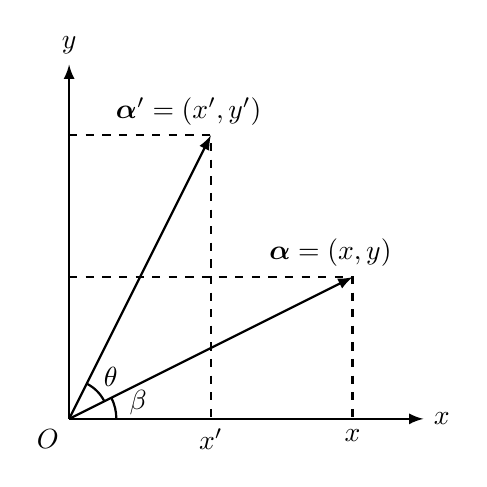
\begin{tikzpicture}[scale=1.8]
                \tikzset{>=latex, every path/.style={thick}}
                \draw (0,0) coordinate (O)
                    (1,2) coordinate (A)
                    (2,1) coordinate (B)
                    (2,0) coordinate (C);
                \draw[->] (0, 0) -- (0, 2.5)
                    node[above] {$y$};
                \draw[->] (0, 0) -- (2.5, 0)
                    node[right] {$x$};
                \draw[->] (O) -- (A)
                    node[above,xshift=-8pt] {$\boldsymbol{\alpha}'=(x',y')$};
                \draw[->] (O) -- (B)
                    node[above,xshift=-8pt] {$\boldsymbol{\alpha}=(x,y)$};
                \draw[dashed] (0,2) -- (1,2) -- (1,0) node[below] {$x'$}
                    (0,1) -- (2,1) -- (2,0) node[below] {$x$};
                \draw pic[draw,"$\theta$",angle eccentricity=1.5] {angle=B--O--A};
                \draw pic[draw,"$\beta$",angle eccentricity=1.5,angle radius=.6cm] {angle=C--O--B};
                \draw node[below left] at (O) {$O$};
            \end{tikzpicture}
        \end{center}
        \item 镜像变换(或镜面反射)--$\mathbf{R}^2$中每个向量关于过原点的直线$L$(看作镜面)相对称的变换 $\varphi$,即
        \[
        \varphi: \forall \alpha = \vec{OA} \in \mathbf{R}^2,\\
        \varphi(\alpha) = \alpha'= \vec{OB}
        \]
        \begin{center}
            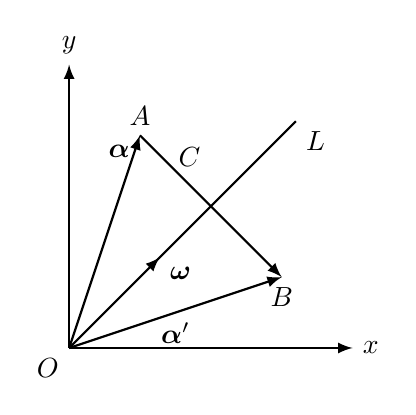
\begin{tikzpicture}[scale=1.8]
                \tikzset{>=latex, every path/.style={thick}, ->-/.style={
                    decoration={markings, mark=at position .4 with {\arrow{>}}}, postaction={decorate}
                }}
                \draw[->] (0, 0) -- (0, 2) node[above] {$y$};
                \draw[->] (0, 0) -- (2, 0) node[right] {$x$};
                \draw (0,0) coordinate (O)
                    (0.5, 1.5) coordinate (A)
                    (1.5,0.5) coordinate (B);
                \draw node[above] at (A) {$A$}
                    node[below left] at (A) {$\boldsymbol{\alpha}$}
                    node[below] at (B) {$B$};
                \draw[->] (O) -- (A);
                \draw[->] (O) -- (B)
                    node[pos=.5, below] {$\boldsymbol{\alpha}'$};
                \draw[->] (A) -- (B)
                    node[pos=.35, above=3pt] {$C$};
                \draw[->-] (O) -- (1.6, 1.6)
                    node[pos=.4, below right] {$\boldsymbol{\omega}$}
                    node[below right] {$L$};
                \draw node[below left] at (O) {$O$};
            \end{tikzpicture}
        \end{center}
        \item 三维立体空间中的投影变换也是线性变换,例如$\mathbf{R}^3$到子空间 $W=\spa((1,0,0))$ 的投影变换 $p$.
        \[
        p: \forall \alpha = (x,y,z) \in \mathbf{R}^3,\\
        p(\alpha) = \alpha'= (x,0,0)
        \]
    \end{enumerate}

\end{example}

\begin{solution}
    \begin{enumerate}
     \item 读者易根据线性映射的定义自行验证
     \item 式中的 \( x', y' \) 分别为
     \[
     x' = r \cos(\theta + \beta) = x \cos \theta - y \sin \theta,
     \]
     \[
     y' = r \sin(\theta + \beta) = x \sin \theta + y \cos \theta,
     \]
     其中 \( \beta = \langle \alpha, \vec{\mathbf{O}x} \rangle \),即
     \[
     r_{\theta}(\alpha) = r_{\theta}(x, y) = (x \cos \theta - y \sin \theta, x \sin \theta + y \cos \theta),
     \]
     于是对 \( \alpha_1 = (x_1, y_1), \alpha_2 = (x_2, y_2) \in \mathbf{R}^2 \) 和任意 \( \lambda, \mu \in \mathbf{R} \),
     \[
     r_{\theta}(\lambda \alpha_1 + \mu \alpha_2) = r_{\theta}(\lambda x_1 + \mu x_2, \lambda y_1 + \mu y_2)
     \]
     \[
     = ((\lambda x_1 + \mu x_2) \cos \theta - (\lambda y_1 + \mu y_2) \sin \theta,
     (\lambda x_1 + \mu x_2) \sin \theta + (\lambda y_1 + \mu y_2) \cos \theta)
     \]
     \[
     = \lambda (x_1 \cos \theta - y_1 \sin \theta, x_1 \sin \theta + y_1 \cos \theta)
     + \mu (x_2 \cos \theta - y_2 \sin \theta, x_2 \sin \theta + y_2 \cos \theta)
     \]
     \[
     = \lambda r_{\theta}(x_1, y_1) + \mu r_{\theta}(x_2, y_2) = \lambda r_{\theta}(\alpha_1) + \mu r_{\theta}(\alpha_2),
     \]
     故 \( r_{\theta} \) 是 \( \mathbf{R}^2 \) 上的一个线性变换.

    \item 证明涉及内积的知识,我们放在\autoref{ex:镜像变换}中讨论.
    \item 读者可以自行验证.
    \end{enumerate}

\end{solution}

除了以上的例子之外,我们也提倡读者了解其它常见的线性映射,特别是具有几何意义的例子(虽然不会直接考察,但是对理解有帮助).例如错切变换与伸缩变换的线性性,或者直接搜索仿射变换的相关内容.

\begin{example}{}{}
    写出下列映射的出发空间和到达空间,并判断其是否为线性映射:
    \begin{enumerate}
        \item $\sigma(x_1,x_2)=(x_1-x_2,x_1,x_1+x_2)$;

        \item $\sigma(x_1,x_2)=(x_1x_2,x_1+x_2)$;

        \item $\sigma(p(x))=p(x+1)-p(x),\enspace\forall p(x) \in \mathbf{R}[x]_n$;

        \item $\sigma(p(x))=p(a),\enspace\forall p(x)$,其中$a$为常数;

        \item $\sigma(\xi)=2\xi+\xi_0$,其中$\xi_0$是线性空间$V$中的一个固定向量.
    \end{enumerate}
\end{example}

\begin{solution}
    \begin{enumerate}
        \item 出发空间为 $ \mathbf{R}^2 $,到达空间为 $ \mathbf{R}^3 $. $ \sigma $ 是线性映射.

              $ \forall (x_1, x_2), (y_1, y_2) \in \mathbf{R}^2,\enspace k_1, k_2 \in \mathbf{R} $, 有
              \begin{align*}
                      & \sigma(k_1(x_1, x_2) + k_2(y_1, y_2))                                                                     \\
                  ={} & ((k_1 x_1 + k_2 y_1) - (k_1 x_2 + k_2 y_2), k_1 x_1 + k_2 y_1, (k_1 x_1 + k_2 y_1) + (k_1 x_2 + k_2 y_2)) \\
                  ={} & k_1(x_1 - x_2, x_1, x_1 + x_2) + k_2(y_1 - y_2, y_1, y_1 + y_2)                                           \\
                  ={} & k_1 \sigma(x_1, x_2) + k_2 \sigma(y_1, y_2)
              \end{align*}

        \item 出发空间为 $ \mathbf{R}^2 $,到达空间为 $ \mathbf{R}^2 $. $ \sigma $ 不是线性映射.

              $ \forall (x_1, x_2), (y_1, y_2) \in \mathbf{R}^2,\enspace k_1, k_2 \in \mathbf{R} $, 有
              \begin{align*}
                  \sigma((x_1, x_2) + (y_1, y_2))
                   & = \sigma(x_1 + y_1, x_2 + y_2)                                        \\
                   & = ((x_1 + y_1)(x_2 + y_2), ((x_1 + y_1) + (x_2 + y_2))                \\
                   & = (x_1 x_2 + x_1 y_2 + y_1 x_2 + y_1 y_2, x_1 + y_1 + x_2 + y_2)      \\
                   & = (x_1 x_2 + y_1 y_2, x_1 + y_1 + x_2 + y_2) + (x_1 y_2 + y_1 x_2, 0) \\
                   & = \sigma(x_1, x_2) + \sigma(y_1, y_2) + (x_1 y_2 + y_1 x_2, 0)        \\
                   & \neq \sigma(x_1, x_2) + \sigma(y_1, y_2)
              \end{align*}

        \item 出发空间为 $ \mathbf{R}[x]_n $,到达空间为 $ \mathbf{R}[x]_{n - 1} $. $ \sigma $ 是线性映射.

              $ \forall p_1(x), p_2(x) \in \mathbf{R}[x]_n,\enspace k_1, k_2 \in \mathbf{R} $, 有
              \begin{align*}
                      & \sigma(k_1 p_1(x) + k_2 p_2(x))                     \\
                  ={} & (k_1 p_1 + k_2 p_2)(x + 1) - (k_1 p_1 + k_2 p_2)(x) \\
                  ={} & k_1(p_1(x + 1) - p_1(x)) + k_2(p_2(x + 1) - p_2(x)) \\
                  ={} & k_1 \sigma(p_1(x)) + k_2 \sigma(p_2(x))
              \end{align*}

        \item 出发空间为 $ \mathbf{R}[x] $,到达空间为 $ \mathbf{R}[x] $. $ \sigma $ 是线性映射.

              $ \forall p_1(x), p_2(x) \in \mathbf{R}[x],\enspace k_1, k_2 \in \mathbf{R} $, 有
              \begin{align*}
                      & \sigma(k_1 p_1(x) + k_2 p_2(x))         \\
                  ={} & (k_1 p_1 + k_2 p_2)(a)                  \\
                  ={} & k_1 p_1(a) + k_2 p_2(a)                 \\
                  ={} & k_1 \sigma(p_1(x)) + k_2 \sigma(p_2(x))
              \end{align*}

        \item 出发空间为 $ V $,到达空间为 $ V $. 当 $ \xi_0 = \vec{0} $ 时, $ \sigma(\xi) = 2 \xi $ 是线性映射.

              $ \forall \xi_1, \xi_2 \in V $, 有
              \begin{align*}
                  \sigma(\xi_1 + \xi_2) & = 2(\xi_1 + \xi_2)              \\
                                        & = 2 \xi_1 + 2 \xi_2             \\
                                        & = \sigma(\xi_1) + \sigma(\xi_2)
              \end{align*}

              当 $ \xi_0 \neq \vec{0} $ 时, $ \sigma $ 不是线性映射.

              $ \forall \xi_1, \xi_2 \in V $, 有
              \begin{align*}
                  \sigma(\xi_1 + \xi_2) & = 2(\xi_1 + \xi_2) + \xi_0              \\
                                        & = 2 \xi_1 + 2 \xi_2 + \xi_0             \\
                                        & = \sigma(\xi_1) + \sigma(\xi_2) - \xi_0 \\
                                        & \neq \sigma(\xi_1) + \sigma(\xi_2)
              \end{align*}
    \end{enumerate}
\end{solution}

\subsection{线性映射的基本运算}

我们在之前的学习中已经了解,连续函数关于函数的加法数乘运算可以构成线性空间,事实上线性映射可以视为特殊的函数,因此我们希望在本节讨论怎样的运算定义能使其构成线性空间,除此之外也介绍线性映射乘法(即复合)和逆运算.

我们需要首先说明一个记号,我们把线性空间$V_1(\mathbf{F})$到$V_2(\mathbf{F})$的所有线性映射组成的集合记作$\mathcal{L}(V_1,V_2)$(类似于将定义在$[a,b]$上取值于实数集的连续函数全体记为$C[a,b]$). 如果是出发空间与到达空间均为$V$的线性变换全体,我们可以简记为$\mathcal{L}(V)$. 我们希望在该集合上定义线性空间,于是需要定义其中元素(线性映射)的加法和数乘运算:
\begin{definition}{}{}
    设$\sigma,\tau\in \mathcal{L}(V_1,V_2)$,规定$\sigma$与$\tau$之和及$\lambda$与$\sigma$的数乘$\lambda\sigma$分别为
    \begin{gather*}
        (\sigma+\tau)(\alpha)=\sigma(\alpha)+\tau(\alpha),\enspace\forall\alpha\in V_1 \\
        (\lambda\sigma)(\alpha)=\lambda(\sigma(\alpha)),\enspace\forall\alpha\in V_1
    \end{gather*}
\end{definition}

不难验证,这样定义的线性映射加法和数乘的结果仍然是线性映射:
\begin{proof}
\begin{enumerate}
    \item 首先证明加法,直接验证即可:
    \begin{align*}
        (\sigma + \tau)(\lambda_1 \alpha_1 + \lambda_2 \alpha_2) & = \sigma(\lambda_1 \alpha_1 + \lambda_2 \alpha_2) + \tau(\lambda_1 \alpha_1 + \lambda_2 \alpha_2) \\
        & = \lambda_1 \sigma(\alpha_1) + \lambda_2 \sigma(\alpha_2) + \lambda_1 \tau(\alpha_1) + \lambda_2 \tau(\alpha_2) \\
        & = \lambda_1 (\sigma(\alpha_1) + \tau(\alpha_1)) + \lambda_2 (\sigma(\alpha_2) + \tau(\alpha_2)) \\
        &= \lambda_1 (\sigma+\tau)(\alpha_1) + \lambda_2 (\sigma+\tau)(\alpha_2).
    \end{align*}

    \item 再证明数乘,同样直接验证即可:
    \begin{align*}
        (\lambda \sigma)(\lambda_1 \alpha_1 + \lambda_2 \alpha_2) & = \lambda \sigma(\lambda_1 \alpha_1 + \lambda_2 \alpha_2) \\
        & = \lambda (\lambda_1 \sigma(\alpha_1) + \lambda_2 \sigma(\alpha_2)) \\
        & = \lambda_1 (\lambda \sigma(\alpha_1)) + \lambda_2 (\lambda \sigma(\alpha_2)) \\
        & = \lambda_1 (\lambda \sigma)(\alpha_1) + \lambda_2 (\lambda \sigma)(\alpha_2).
    \end{align*}
\end{enumerate}
\end{proof}

进一步地,线性空间 $V_1(\mathbf{F})$ 到 $V_2(\mathbf{F})$ 的所有线性映射 $\mathcal{L}(V_1,V_2)$ 关于上面定义的加法和数乘构成线性空间:

\begin{theorem}{}{线性映射全体构成线性空间}
    $\mathcal{L}(V_1,V_2)$与上述定义的线性映射加法和数乘构成域$\mathbf{F}$上的线性空间.
\end{theorem}

实际上,前面我们证明的线性映射加法和数乘的结果仍然是线性映射,就是线性映射的加法和数乘的封闭性,因此我们只需证明线性映射的加法和数乘满足线性空间的 8 条性质即可. 事实上这是非常显然的,我们只需注意 $\mathcal{L}(V_1,V_2)$ 中的零元就是零映射 $\theta$(将 $V_1$ 中的任意元素都映射到 $V_2$ 中的零元)即可,因此我们不再赘述.

下面讨论线性映射的其它运算. 首先是复合运算. 设$\sigma \in \mathcal{L}(V_1,V_2),\enspace\tau \in \mathcal{L}(V_2,V_3)$,则$\tau\sigma$是$\mathcal{L}(V_1,V_3)$中的元素,且$\tau\sigma(\alpha)=\tau(\sigma(\alpha)),\enspace\forall \alpha \in V_1$.

\begin{theorem}{}{复合映射是线性映射}
    上述定义的映射 $\tau\sigma$ 是线性映射.
\end{theorem}

注意:在上述定义中一定注意$\sigma$和$\tau$的顺序,我们需要先使用$\sigma$将$V_1$中的元素映射到$V_2$,然后再用外层的$\tau$将这个结果映射到$V_3$. 此外,有时也会将复合映射记作$\tau \circ \sigma$(一般是为了强调这是复合运算),这里为了简化记号直接使用$\tau\sigma$.

接下来定义线性映射的逆运算,也就是定义逆映射,事实上与反函数的定义类似. 设 $\sigma \in \mathcal{L}(V_1,V_2)$. 若存在 $\tau \in \mathcal{L}(V_2,V_1)$ 使得 $\sigma \tau = I_{V_2}$ 且 $\tau \sigma = I_{V_1}$,则称 $\sigma$\term{可逆}\index{ni!ke@可逆 (invertible)},并称 $\tau$ 为 $\sigma$ 的逆映射\index{ni!yingshe@映射 (inverse map)}. 其中 $I_{V_1}$ 和 $I_{V_2}$ 分别是 $V_1$ 和 $V_2$ 上的恒等映射,即 $I_{V_i}(\alpha)=\alpha,\enspace \forall \alpha \in V_i,\ i = 1, 2$.

\begin{theorem}{}{逆映射是线性映射}
    上述定义的逆映射 $\sigma^{-1}$ 为线性映射.
\end{theorem}

\autoref{thm:复合映射是线性映射}和\autoref{thm:逆映射是线性映射}的证明是非常基本的,在阅读详细的证明之前,读者可以先自行尝试,如果不会证明则说明对于线性空间和线性映射的定义熟悉程度仍需提高,因为这里的证明都只需要机械地套用定义.

\begin{proof}
\begin{enumerate}
    \item 如果 $\sigma_1$ 和 $\sigma_2$ 分别是线性空间 $V_1(F)$ 到 $V_2(F)$ 和 $V_2(F)$ 到 $V_3(F)$ 的线性映射,那么
    \begin{align*}
        (\sigma_2 \circ \sigma_1)(\lambda \alpha  + \mu \beta) & = \sigma_2(\sigma_1(\lambda \alpha  + \mu \beta)) \\
        & = \sigma_2(\lambda (\sigma_1(\alpha))) + \mu_1(\sigma_1(\beta)) \\
        & = \lambda (\sigma_2(\sigma_1)(\alpha)) + \mu (\sigma_2(\sigma_1)(\beta)),
    \end{align*}
    所以 $\sigma_2\sigma_1$ 是 $V_1$ 到 $V_3$ 的线性映射.

    \item 如果可逆线性映射 $\sigma: V_1 \to V_2$ 的逆映射为 $\sigma^{-1}: V_2 \to V_1$,那么
    \[
    \sigma^{-1} \circ \sigma = I_{V_1}, \quad \text{且} \quad \sigma \circ \sigma^{-1} = I_{V_2},
    \]
    于是对于$ \forall \beta_1,\beta_2 \in V_2$和任意的标量 $\lambda_1, \lambda_2 \in F$,有
    \begin{align*}
        \sigma^{-1}(\lambda_1 \beta_1 + \lambda_2 \beta_2) & = \sigma^{-1}\left[ \lambda_1(\sigma \sigma^{-1})(\beta_1)+\lambda_2(\sigma \sigma^{-1})(\beta_2)\right] \\
        &= \sigma^{-1}(\lambda_1 \sigma(\sigma^{-1}(\beta_1)) + \lambda_2 \sigma(\sigma^{-1}(\beta_2))) \\
        & = \lambda_1 \sigma^{-1}(\beta_1) + \lambda_2 \sigma^{-1}(\beta_2),
    \end{align*}
    所以 $\sigma^{-1}$ 是线性的.
\end{enumerate}
\end{proof}

除此之外,关于线性映射的复合,我们还有结合律,即 $\tau(\sigma\eta) = (\tau\sigma)\eta$,这是显然的,因为
\[\tau(\sigma\eta)(\alpha) = \tau((\sigma\eta)(\alpha)) = \tau(\sigma(\eta(\alpha))) = (\tau\sigma)(\eta(\alpha)) = (\tau\sigma)\eta(\alpha).\]
这与普通函数的复合运算满足结合律没有任何区别.

\section{线性映射的像与核}

我们在之前的讨论中已经了解了线性映射的定义与运算,接下来我们需要关心的问题是:定义出的线性映射能将出发空间完整映射到到达空间吗,还是到达空间中有些向量无法被映到?线性映射是否可以是单射?单射的充要条件又是什么?这与我们研究一般的映射的思路是类似的. 因此我们希望在本节讨论线性映射的像和核.
\begin{definition}{}{}
    设$\sigma$是线性空间$V_1(\mathbf{F})$到$V_2(\mathbf{F})$的线性映射. $V_1$的所有元素在$\sigma$下的像组成的集合
    \[\sigma(V_1)=\{\beta \mid \beta=\sigma(\alpha),\enspace \alpha \in V_1\}\]
    称为$\sigma$的\term{像}(或\term{值域})\index{xiang@像 (image), 值域 (range)},记作$\im \sigma$,或记作 $\operatorname{range}\sigma$.

    $V_2$的零元$0_2$在$\sigma$下的完全原像
    \[\sigma^{-1}(0_2)=\{\alpha \mid \sigma(\alpha)=0_2,\enspace \alpha \in V_1\}\]
    称为$\sigma$的\term{核}(或\term{零空间})\index{he@核 (kernel), 零空间 (null space)},记作$\ker \sigma$,或记作 $\operatorname{null}\sigma$.
\end{definition}

关于像与核的定义,我们需要强调以下几点:
\begin{enumerate}
    \item 实际上,像空间的定义就类似于函数的值域,核空间可以视为到达空间中0的原像集合,因此理解起来是很简单的;

    \item 注意线性映射的像和核分别是$V_2$和$V_1$的子空间. 同样地,若$W_1$和$W_2$分别是$V_1$和$V_2$的子空间,则$\sigma(W_1)$和$\sigma^{-1}(W_2)$也分别是$V_2$和$V_1$的子空间.我们在此只给出前者的证明,后者我们作为习题留给读者,实际上都非常简单,只是为读者熟悉定义而在此处提及.
          \begin{proof}
              首先我们证明像空间是$V_2$的子空间. 设$\beta_1,\beta_2\in \sigma(V_1)$,则存在$\alpha_1,\alpha_2\in V_1$使得$\beta_1=\sigma(\alpha_1),\beta_2=\sigma(\alpha_2)$,于是
              \[\beta_1+\beta_2=\sigma(\alpha_1)+\sigma(\alpha_2)=\sigma(\alpha_1+\alpha_2)\in \sigma(V_1),\]
              \[\lambda\beta_1=\lambda\sigma(\alpha_1)=\sigma(\lambda\alpha_1)\in \sigma(V_1),\]
              因此$\sigma(V_1)$是$V_2$的子空间.

              接下来我们证明核空间是$V_1$的子空间. 设$\alpha_1,\alpha_2\in \sigma^{-1}(0_2)$,则$\sigma(\alpha_1)=\sigma(\alpha_2)=0_2$,于是
              \[\sigma(\alpha_1+\alpha_2)=\sigma(\alpha_1)+\sigma(\alpha_2)=0_2+0_2=0_2,\]
              \[\lambda\sigma(\alpha_1)=\sigma(\lambda\alpha_1)=0_2,\]
              因此$\sigma^{-1}(0_2)$是$V_1$的子空间.
          \end{proof}
\end{enumerate}

接下来我们要讨论如何计算线性映射的像与核,这在考试中非常常见,请务必牢记,无论线性映射有多么复杂多么抽象,基本的方法都是:
\begin{enumerate}
    \item 设出发空间的一组基为$B=\{\alpha_1,\alpha_2,\ldots,\alpha_n\}$,则像空间
          \[\im \sigma=\sigma(V_1)=\spa(\sigma(\alpha_1),\sigma(\alpha_2),\ldots,\sigma(\alpha_n)).\]
          即线性映射在出发空间一组基下的像的线性扩张,解答时写出极大线性无关组然后扩张即可;

          当然读者可能质疑其合理性,因为与定义不完全一致. 我们可以证明这一方法是合理的,即线性映射在出发空间一组基下像的线性扩张就是其像空间.

          \begin{proof}
              首先我们知道$\sigma(V_1)$包含$\sigma(\alpha_1),\sigma(\alpha_2),\ldots,\sigma(\alpha_n)$,并且是$V_2$的子空间. 又根据\autoref{thm:线性扩张构造子空间},$\sigma(V_1)$是包含$\sigma(\alpha_1),\sigma(\alpha_2),\ldots,\sigma(\alpha_n)$的最小子空间,因此我们可以得到$\spa(\sigma(\alpha_1),\sigma(\alpha_2),\ldots,\sigma(\alpha_n))\subseteq\sigma(V_1)$.

              接下来证明另一半包含. 根据线性扩张定义可知只需证$V_1$中任意元素的像都可以被$\sigma(\alpha_1),\sigma(\alpha_2),\ldots,\sigma(\alpha_n)$线性表示. 任取$\alpha\in V_1$,则$\alpha$可由$V_1$一组基$\{\alpha_1,\alpha_2,\ldots,\alpha_n\}$线性表示为$\alpha=\lambda_1\alpha_1+\lambda_2\alpha_2+\cdots+\lambda_n\alpha_n$,于是,
              \[\sigma(\alpha)=\sigma(\lambda_1\alpha_1+\lambda_2\alpha_2+\cdots+\lambda_n\alpha_n)=\lambda_1\sigma(\alpha_1)+\lambda_2\sigma(\alpha_2)+\cdots+\lambda_n\sigma(\alpha_n)\]
              即$\sigma(\alpha)$可由$\sigma(\alpha_1),\sigma(\alpha_2),\ldots,\sigma(\alpha_n)$线性表示,即出发空间任意向量在$\sigma$下的像都可以由$\sigma(\alpha_1),\sigma(\alpha_2),\ldots,\sigma(\alpha_n)$线性表示,因此$\sigma(V_1)\subseteq\spa(\sigma(\alpha_1),\sigma(\alpha_2),\ldots,\sigma(\alpha_n))$.
          \end{proof}

    \item 核空间可以直接利用定义令$\sigma(\alpha)=0$,利用解线性方程组得到解集即为结果,注意也许表示为线性扩张的形式.
\end{enumerate}

\begin{example}{}{}
    已知$\mathbf{R}^3$到$\mathbf{R}^2$的映射$\sigma$为$\sigma(x_1,x_2,x_3)^{\color{lightgray}\mathrm{T}}=(x_1+x_2,x_2-x_3)^{\color{lightgray}\mathrm{T}}$,求$\sigma$的像和核.
\end{example}
注:这里需要对记号进行一个澄清,事实上 $\mathbf{R}^n$ 空间中的向量都应当是列向量,但为了节省空间,一些教材在描述映射的情形下会写成行向量的形式. 但笔者认为线性映射相关的地方行和列的混乱容易导致一些困惑,为此,笔者有时会在向量的右上角加上一个浅色的转置 $({}^{\color{gray}\mathrm{T}})$ 以代表它是列向量.

\begin{solution}
    \begin{itemize}
        \item 首先求像空间. 取出发空间$\mathbf{R}^3$的一组基$B=\{(1,0,0)^{\color{lightgray}\mathrm{T}},(0,1,0)^{\color{lightgray}\mathrm{T}},(0,0,1)^{\color{lightgray}\mathrm{T}}\}$,则
        \begin{align*}
            \im \sigma &=\sigma(\mathbf{R}^3) = \spa(
                \sigma(1,0,0)^{\color{lightgray}\mathrm{T}},
                \sigma(0,1,0)^{\color{lightgray}\mathrm{T}},
                \sigma(0,0,1)^{\color{lightgray}\mathrm{T}}
                 ) \\
            &=\spa(
                (1,0)^{\color{lightgray}\mathrm{T}},
                (1,1)^{\color{lightgray}\mathrm{T}},
                (0,-1)^{\color{lightgray}\mathrm{T}}
                )
        \end{align*}
        根据求解极大线性无关组的方法(或者这么简单的情况瞪眼法也可以)得到像空间
        $\im \sigma=\spa((1,0)^{\color{lightgray}\mathrm{T}},(0,-1)^{\color{lightgray}\mathrm{T}})=\mathbf{R}^2$.

        \item 接下来求解核空间. 设$\sigma(\alpha)=0$,其中$\alpha=(x_1,x_2,x_3)^{\color{lightgray}\mathrm{T}}$,即$\sigma(x_1,x_2,x_3)^{\color{lightgray}\mathrm{T}}=(x_1+x_2,x_2-x_3)^{\color{lightgray}\mathrm{T}}=(0,0)$,解得解向量为$k(-1,1,1)^{\color{lightgray}\mathrm{T}},\enspace k\in\mathbf{R}$,写成线性扩张的形式为$\spa((-1,1,1)^{\color{lightgray}\mathrm{T}})$.
    \end{itemize}
\end{solution}

下面我们也给出另一种求像空间的方法,但是为了防止读者混淆这一方法和之后线性映射矩阵表示的方法,希望读者能按照笔者首先介绍的方法求解.
\begin{solution}\label{ex:线性映射的像空间求解2}
    \begin{align*}
        \sigma(x_1, x_2, x_3)^{\color{lightgray}\mathrm{T}} &= (x_1 + x_2, x_2 - x_3)^{\color{lightgray}\mathrm{T}}\\
        &= x_1(1, 0)^{\color{lightgray}\mathrm{T}} + x_2(1, 1)^{\color{lightgray}\mathrm{T}} + x_3(0, -1)^{\color{lightgray}\mathrm{T}}
    \end{align*}
    记 $\beta_1 = (1, 0)^{\color{lightgray}\mathrm{T}}, \beta_2 = (1, 1)^{\color{lightgray}\mathrm{T}}, \beta_3 = (0, -1)^{\color{lightgray}\mathrm{T}}$,则 $\sigma(x_1, x_2, x_3)^{\color{lightgray}\mathrm{T}} = x_1 \beta_1 + x_2 \beta_2 + x_3 \beta_3$,所以 $\sigma(\mathbf{R}^3) = \spa\{\beta_1, \beta_2, \beta_3\} = \spa \{\beta_1, \beta_2\}=\mathbf{R}^2$.
\end{solution}


事实上,研究一般映射我们会很在意映射是否为单射或满射. 是否为满射通过我们介绍的求解像空间的方法是很好判断的,但单射似乎并不能直接利用像空间或者核空间直接判断,但我们只需稍作转化就可以发现单射和核空间有着密不可分的联系:
\begin{theorem}{}{单射与核空间}
    线性映射$\sigma$是单射当且仅当$\ker \sigma=\{0\}$.
\end{theorem}
这个定理告诉我们,线性映射是单射和0的逆像只有0是等价的. 这一结论也是非常强的,因为我们知道一般的函数是不满足这一结论的,例如$f(x)=x^2$,虽然只有$f(0)=0$,但在$\mathbf{R}$上显然不是单射. 这一定理证明非常简单,希望读者掌握:

\begin{proof}
    首先我们证明$\sigma$是单射时$\ker\sigma=\{0\}$. 事实上$\sigma$是单射意味着任意到达空间中的元素的逆象唯一,又线性映射必须满足$\sigma(0)=0$,则0的逆象唯一为0是显然的.

    接下来我们证明$\ker \sigma=\{0\}$时$\sigma$是单射. 事实上,$\sigma(\alpha)=\sigma(\beta)$等价于$\sigma(\alpha)-\sigma(\beta)=0$,即$\sigma(\alpha-\beta)=0$,由于$\ker \sigma=\{0\}$,因此$\alpha-\beta=0$,即$\alpha=\beta$,因此$\sigma$是单射.
\end{proof}

\section{线性映射的确定}

我们知道,两个函数相等当且仅当它们的定义域相等且对于任意定义域内的元素,它们的函数值相等. 线性映射则有更好的性质,即有限维空间上的线性映射可以被基上的像唯一确定,即
\begin{theorem}{}{线性映射唯一确定}
    已知线性映射$\sigma,\tau\in \mathcal{L}(V_1,V_2)$,且有$V_1$的基$B=\{\alpha_1,\alpha_2,\ldots,\alpha_n\}$. 若$\sigma(\alpha_i)=\tau(\alpha_i),\enspace\forall \alpha_i \in B$,则有$\sigma=\tau$.
\end{theorem}
即映射在一组基上的像确定了,则映射是唯一的. 证明非常简单:

\begin{proof}
    实际上我们只需证明$\sigma(\alpha)=\tau(\alpha),\enspace\forall \alpha \in V_1$即可,因为这就是一般映射相等的条件. 事实上,任取$\alpha \in V_1$,则$\alpha$可由$B$线性表示为$\alpha=\lambda_1\alpha_1+\lambda_2\alpha_2+\cdots+\lambda_n\alpha_n$,于是
    \begin{gather*}
        \sigma(\alpha)=\sigma(\lambda_1\alpha_1+\lambda_2\alpha_2+\cdots+\lambda_n\alpha_n)=\lambda_1\sigma(\alpha_1)+\lambda_2\sigma(\alpha_2)+\cdots+\lambda_n\sigma(\alpha_n) \\
        \tau(\alpha)=\tau(\lambda_1\alpha_1+\lambda_2\alpha_2+\cdots+\lambda_n\alpha_n)=\lambda_1\tau(\alpha_1)+\lambda_2\tau(\alpha_2)+\cdots+\lambda_n\tau(\alpha_n)
    \end{gather*}
    由于$\sigma(\alpha_i)=\tau(\alpha_i),\enspace\forall \alpha_i \in B$,因此$\sigma(\alpha)=\tau(\alpha)$,即$\sigma=\tau$.
\end{proof}

事实上这与之前证明求解像空间的方法合理性(即证线性映射在一组基上的像的线性扩张就是线性映射的像空间)是完全相通的. 这里也蕴含了一个数学的基本想法. 我们发现线性映射比一般的函数要求更高,因为它要求了两个运算性质,我们说这里构成线性映射的条件比构成一般函数的条件``更强''. 更强的要求必然带来更美妙的结果,例如线性映射可被基上的像唯一确定,而一般函数则不存在这样的性质. 抑或是未来如果有同学学习复变函数时,那时我们研究的``全纯函数''比数学分析中常见的连续函数要求更强,因此会有大量在数学分析中无法想象的非常漂亮的结果. 值得一提的是,复变函数这样美妙的结果直接带来了\nameref{thm:代数学基本定理}的非常简便的证明,这在数学史上是非常重要的里程碑.

\begin{theorem}{}{线性映射构造}
    设$B=\{\alpha_1,\alpha_2,\ldots,\alpha_n\}$是$V_1$的基,$S=\{\beta_1,\beta_2,\ldots,\beta_n\}$是$V_2$中任意$n$个向量,则存在唯一的$\sigma\in \mathcal{L}(V_1,V_2)$使得$\sigma(\alpha_i)=\beta_i,\enspace i=1,2,\ldots,n$.
\end{theorem}

\begin{proof}
这一定理的证明也是简单的,只需先定义出这个映射. $\forall \alpha \in V_1$,则$\alpha$可由$B$线性表示为$\alpha=\lambda_1\alpha_1+\lambda_2\alpha_2+\cdots+\lambda_n\alpha_n$,于是定义
\[\sigma(\alpha)=\sigma(\lambda_1\alpha_1+\lambda_2\alpha_2+\cdots+\lambda_n\alpha_n)=\lambda_1\beta_1+\lambda_2\beta_2+\cdots+\lambda_n\beta_n\]
即可满足条件,因为我们可以验证这是线性映射:

\[
\forall \enspace \xi_1, \xi_2 \in V_1, \lambda_1, \lambda_2 \in F
\]
\[
\begin{cases}
    \xi_1 = x_1\alpha_1+x_2\alpha_2+\cdots+x_n\alpha_n,\\
    \xi_2 = y_1\alpha_1+y_2\alpha_2+\cdots+y_n\alpha_n
\end{cases}
\]
\begin{align*}
\sigma(\lambda_1 \xi_1 + \lambda_2 \xi_2) &= \sigma(\lambda_1(x_1\alpha_1+x_2\alpha_2+\cdots+x_n\alpha_n) + \lambda_2(y_1\alpha_1+y_2\alpha_2+\cdots+y_n\alpha_n))\\
&= \lambda_1(x_1\beta_1+x_2\beta_2+\cdots+x_n\beta_n) + \lambda_2(y_1\beta_1+y_2\beta_2+\cdots+y_n\beta_n)\\
&= \lambda_1\sigma(\xi_1) + \lambda_2\sigma(\xi_2)
\end{align*}

并且唯一性在\autoref{thm:线性映射唯一确定} 中已经说明. 实际上对于初学而言难点在于定义,实际上证明后会发现这一定义太自然了,就是向着线性性定义的,因此很多构造不需要太复杂的想法,自然的、满足要求的是最好的.
\end{proof}
最后我们讨论一个初学时容易困惑的问题,如下例所示:
\begin{example}{}{线性映射判断1}
    是否存在$\mathbf{R}^2$到$\mathbf{R}^3$的线性映射$\sigma$使得$\sigma(1,0)^{\color{lightgray}\mathrm{T}}=(1,0,0)^{\color{lightgray}\mathrm{T}},\enspace\sigma(0,1)^{\color{lightgray}\mathrm{T}}=(0,1,0)^{\color{lightgray}\mathrm{T}},\enspace\sigma(1,1)^{\color{lightgray}\mathrm{T}}=(0,0,1)^{\color{lightgray}\mathrm{T}}$?
\end{example}

初学时感到困难是因为不能熟练应用线性映射的各类性质,找不到映射定义也不敢下结论不存在,或者发现必要条件都满足了却不敢构造. 我们这里给出几个解决策略:
\begin{enumerate}
    \item \label{item:5:线性映射判断1:1}
          根据\autoref{thm:线性映射零元性质} 可知,如果我们发现题目给定的条件无法满足将出发空间零元映射至到达空间零元则一定不是线性映射;

    \item \label{item:5:线性映射判断1:2}
          根据\autoref{thm:线性映射保相关性} 可知,如果我们发现映射将线性相关的向量组映射到了线性无关向量组,则一定不是线性映射;

    \item \label{item:5:线性映射判断1:3}
          不存在从低维线性空间到高维线性空间的满射,原因是简单的:取低维出发空间的一组基$B=\{\alpha_1,\alpha_2,\ldots,\alpha_m\}$,则基下的像的线性扩张$\spa(\sigma(\alpha_1),\sigma(\alpha_2),\ldots,\sigma(\alpha_m))$就是像空间. 我们取高维到达空间的一组基$B_2=\{\beta_1,\beta_2,\ldots,\beta_n\}$,则由于维数更高有$n>m$. 由于$\sigma$是满射,因此$\sigma(\alpha_1),\sigma(\alpha_2),\ldots,\sigma(\alpha_m)$可以线性表示出$B_2$中任意向量,根据\autoref{thm:线性表示} 可知(这是长的向量可以被短的向量线性表示),向量组$B_2$线性相关,但我们知道这是一组基,因此矛盾!

          这一性质在下一讲介绍了线性映射基本定理后会有更简单的证明,但此处的证明也是很重要的,体现了\autoref{thm:线性表示} 作为源泉定理的重要性.

    \item 如果题目给定的映射不违反上述线性映射的必要条件,那我们可以按照\autoref{thm:线性映射构造} 构造出相应的映射.
\end{enumerate}

根据上面的描述,我们发现 \ref*{item:5:线性映射判断1:1} 中的映射定义违反了明显违反了不能是从低维到高维满射的条件. 实际上,$\sigma$也将线性相关的向量组映射到了线性无关的向量组,并且根据定义,$\sigma(0)=\sigma((1,0)^{\color{lightgray}\mathrm{T}}+(0,1)^{\color{lightgray}\mathrm{T}}-(1,1)^{\color{lightgray}\mathrm{T}})=(1,1,-1)$,因此所有的必要条件都被违反了,因此这一映射一定不是线性映射. 事实上这一例子也表明很多时候三个必要条件可能是同时违反的,因为它们都是由基本的线性映射和线性相关性质推导而来,并非完全独立的判据.

我们还需强调的是,如果\autoref{thm:线性映射构造} 前提成立,即题目给我们的是一组基下的像,则一定不会违反上述三个必要条件. 对于条件 \ref*{ex:线性映射判断1},给定一组基$\alpha_1,\ldots,\alpha_n$,我们要凑出$\sigma(0)$只能通过$\sigma(0)=\sigma(0\alpha_1+\cdots+0\alpha_n)=0\sigma(\alpha_1)+\cdots+0\sigma(\alpha_n)=0$,因此不可能违反  \ref*{item:5:线性映射判断1:1}. 对于 \ref*{item:5:线性映射判断1:2},我们给定的是基,因此不存在将线性相关向量组映射到线性无关向量组的情况. 对于 \ref*{item:5:线性映射判断1:3},如果题目给出的是低维到高维的映射,由于我们只给出了低维出发空间的基下的像,这些像不可能张成整个高维到达空间(原理和$n-1$个向量无法张成$n$维空间一致),因此也不可能违反 \ref*{item:5:线性映射判断1:3},因此\autoref{thm:线性映射构造} 并不与我们的必要条件相矛盾,相反,如果题目给出的是一组基下的像,我们就可以毫无顾虑地说映射一定存在.

最后我们再看一个例子来练习我们上面的策略:
\begin{example}{}{线性映射判断2}
    是否存在$\mathbf{R}^3$到$\mathbf{R}^2$的线性映射$\sigma$使得$\sigma(1,-1,1)^{\color{lightgray}\mathrm{T}}=(1,0)^{\color{lightgray}\mathrm{T}},\enspace\sigma(1,1,1)^{\color{lightgray}\mathrm{T}}=(0,1)^{\color{lightgray}\mathrm{T}}$?
\end{example}

\begin{solution}
    事实上这里的定义完全不违反上述的必要条件,因此我们考虑证明这一线性映射存在. 根据\autoref{thm:线性映射构造},我们考虑构造出$\sigma$在一组基(我们取自然基)下的像,然后我们就可以根据\autoref*{thm:线性映射构造} 知道这一映射一定存在.

    实际上,根据提给条件我们有
    \begin{gather*}
        \sigma(1,-1,1)^{\color{lightgray}\mathrm{T}}
        =\sigma(e_1-e_2+e_3)
        =\sigma(e_1)-\sigma(e_2)+\sigma(e_3)
        =(1,0)^{\color{lightgray}\mathrm{T}} \\
        \sigma(1,1,1)^{\color{lightgray}\mathrm{T}}
        =\sigma(e_1+e_2+e_3)
        =\sigma(e_1)+\sigma(e_2)+\sigma(e_3)
        =(0,1)^{\color{lightgray}\mathrm{T}}
    \end{gather*}
    我们希望解出$\sigma(e_1),\sigma(e_2),\sigma(e_3)$,这样就可以直接根据\autoref*{thm:线性映射构造} 构造出这一线性映射. 但这一方程组只有2个方程却有三个未知量. 事实上我们可以任意定义$\sigma(e_3)=(0,0)$,然后解方程组得到
    \[\sigma(e_1)=\dfrac{1}{2} (1,1)^{\color{lightgray}\mathrm{T}},\enspace \sigma(e_2)=\dfrac{1}{2} (-1,1)^{\color{lightgray}\mathrm{T}}\]
    又由$\sigma(e_3)=(0,0)^{\color{lightgray}\mathrm{T}}$,根据\autoref*{thm:线性映射构造},满足题目条件的线性映射存在.
\end{solution}
需要注意的是题目中$\sigma(e_3)$不一定要定义为$(0,0)$,这样只是为了计算方便,事实上定义成任何值都可以得到$\sigma$在一组基下的像,从而根据\autoref*{thm:线性映射构造} 得到这一线性映射存在. 如果题目要求我们写出映射也并不复杂,根据我们在\autoref*{thm:线性映射构造} 中的构造方法,我们可以写出$\forall\alpha=(x,y,z)=xe_1+ye_2+ze_3$,
\[
    \sigma(\alpha)
    =\sigma(xe_1+ye_2+ze_3)
    =x\sigma(e_1)+y\sigma(e_2)+z\sigma(e_3)
    =\dfrac{1}{2} (x-y,x+y)^{\color{lightgray}\mathrm{T}}
\]
符合题目条件. 事实上根据$\sigma(e_3)$定义的不唯一,我们可以得到不同的线性映射,这里只是给出一种可能的解.

\section{线性映射基本定理}

\subsection{线性映射基本定理的陈述与证明}

本节将要介绍的定理是线性代数最重要的定理之一,因其重要性也被冠以(有限维线性空间)线性映射基本定理的名号. 为了介绍这一定理,我们需要首先引入一个概念:线性映射的秩. 在线性映射像求解的讨论中我们有$\im \sigma=\sigma(V_1)=\spa(\sigma(\alpha_1),\sigma(\alpha_2),\ldots,\sigma(\alpha_n))$. 我们基于此定义线性映射的秩:
\begin{definition}{}{}
    设$\sigma\in \mathcal{L}(V_1,V_2)$,如果$\sigma(V_1)$是$V_2$的有限维子空间,则$\sigma(V_1)$的维数称为$\sigma$的秩,记作$r(\sigma)$,即$r(\sigma)=\dim \sigma(V_1)$.
\end{definition}

这一定义是平凡的,简单理解线性映射的秩即为线性映射像空间的维数. 基于这一定理我们便可以介绍本节的核心定理:

\begin{theorem}{线性映射基本定理}{线性映射基本定理}
    设$\sigma \in \mathcal{L}(V_1,V_2)$,若$\dim V_1=n$,则
    \[r(\sigma)+\dim\ker\sigma=n.\]
\end{theorem}
简而言之,这一定理表明:线性映射的秩(或者说线性映射像空间维数)与核空间维数之和等于出发空间的维数. 这一定理的证明非常重要,在之后的很多讨论中还会用到这一思想,因此我们给出详细的证明并阐述其中的思想:

\begin{proof}
    证明的思路和\nameref{thm:线性空间维数公式}的证明思路类似,即``设小扩大''.

    我们设$\dim\ker\sigma=k$,并设$\ker\sigma$的一组基为$\alpha_1,\alpha_2,\ldots,\alpha_k$. 我们将其扩充为$V_1$的一组基,记为$\alpha_1,\alpha_2,\ldots,\alpha_k,\alpha_{k+1},\ldots,\alpha_n$.

    根据定理要证明的等式和前述假设,我们只需证$r(\sigma)=n-k$,即证明像空间维数为$n-k$. 我们知道像空间为$\spa(\sigma(\alpha_1),\sigma(\alpha_2),\ldots,\sigma(\alpha_n))$,其中根据我们的假设,$\sigma(\alpha_1)=\sigma(\alpha_2)=\cdots=\sigma(\alpha_k)=0$(因为它们是核空间的基),因此像空间为$\spa(\sigma(\alpha_{k+1}),\ldots,\sigma(\alpha_n))$. 我们只需证明这一向量组是线性无关的即可,因为这样这$n-k$个向量就可以构成像空间的一组基,从而证明了$r(\sigma)=n-k$.

    我们设$c_{k+1}\sigma(\alpha_{k+1})+\cdots+c_n\sigma(\alpha_n)=0$,即
    \[\sigma(c_{k+1}\alpha_{k+1}+\cdots+c_n\alpha_n)=0\]
    故$c_{k+1}\alpha_{k+1}+\cdots+c_n\alpha_n \in \ker\sigma$,因此可以被$\alpha_1,\alpha_2,\ldots,\alpha_k$线性表示. 于是有
    \[c_{k+1}\alpha_{k+1}+\cdots+c_n\alpha_n=c_1\alpha_1+\cdots+c_k\alpha_k\]
    即
    \[c_1\alpha_1+\cdots+c_k\alpha_k-c_{k+1}\alpha_{k+1}-\cdots-c_n\alpha_n=0\]
    由于$\alpha_1,\alpha_2,\ldots,\alpha_n$是$V_1$的一组基,因此$c_1=\cdots=c_k=c_{k+1}=\cdots=c_n=0$,故$\sigma(\alpha_{k+1}),\ldots,\sigma(\alpha_n)$线性无关,命题得证.
\end{proof}

事实上这一定理也被称为线性映射``维数公式'',但为了与\nameref{thm:线性空间维数公式}区分,本讲义中我们称这一定理为线性映射基本定理. 读者可以比较一下两个``维数公式''的证明,二者都使用了``设小扩大''的思想,都将要证明的结论转化为证明一组向量是线性无关的,但其中证明线性无关的方法略有不同,读者可以仔细体会.

下面我们给出一个证明思想上类似的例子供读者练习:
\begin{example}{}{}
    设$\sigma$为有限维线性空间$V$上的线性变换,$W$是$V$的子空间,证明:
    \[\dim\sigma(W)+\dim(\ker\sigma \cap W)=\dim W.\]
\end{example}

\begin{proof}
    与\nameref{thm:线性映射基本定理}证明类似,我们``设小扩大''. 设$\dim W=n,\enspace\dim\ker\sigma\cap W=k$,设$\ker\sigma\cap W$的一组基为$\alpha_1,\alpha_2,\ldots,\alpha_k$,我们将其扩充为$W$的一组基,记为
    \[\alpha_1,\alpha_2,\ldots,\alpha_k,\alpha_{k+1},\ldots,\alpha_n.\]

    根据定理要证明的等式和前述假设,我们只需证$\dim\sigma(W)=n-k$. 我们知道像空间为$\sigma(W)=\spa(\sigma(\alpha_1),\sigma(\alpha_2),\ldots,\sigma(\alpha_n))$,其中根据我们的假设,$\sigma(\alpha_1)=\sigma(\alpha_2)=\cdots=\sigma(\alpha_k)=0$,因此像空间为$\spa(\sigma(\alpha_{k+1}),\ldots,\sigma(\alpha_n))$. 我们只需证明这一向量组是线性无关的即可,因为这样这$n-k$个向量就可以构成像空间的一组基,从而证明了$\dim\sigma(W)=n-k$.

    我们设
    \[c_{k+1}\sigma(\alpha_{k+1})+\cdots+c_n\sigma(\alpha_n)=0,\]
    即$\sigma(c_{k+1}\alpha_{k+1}+\cdots+c_n\alpha_n)=0$,故$c_{k+1}\alpha_{k+1}+\cdots+c_n\alpha_n\in\ker\sigma$,因此可以被$\alpha_1,\alpha_2,\ldots,\alpha_k$线性表示. 于是有
    \[c_{k+1}\alpha_{k+1}+\cdots+c_n\alpha_n=c_1\alpha_1+\cdots+c_k\alpha_k,\]
    即
    \[c_1\alpha_1+\cdots+c_k\alpha_k-c_{k+1}\alpha_{k+1}-\cdots-c_n\alpha_n=0,\]
    由于$\alpha_1,\alpha_2,\ldots,\alpha_n$是$W$的一组基,因此$c_1=\cdots=c_k=c_{k+1}=\cdots=c_n=0$,故$\sigma(\alpha_{k+1}),\ldots,\sigma(\alpha_n)$线性无关,命题得证.
\end{proof}

基于线性映射基本定理,我们可以得到如下定理:
\begin{theorem}{}{双射等价条件}
    对$\sigma \in \mathcal{L}(V_1,V_2)$且$\dim V_1=\dim V_2=n$,下列条件等价:
    \begin{enumerate}
        \item \label{item:6:双射等价条件:1}
              $\ker \sigma=\{0\}$;

        \item \label{item:6:双射等价条件:2}
              $\sigma$为单射;

        \item $\sigma$为满射;

        \item $\sigma$为双射(可逆);

        \item $r(\sigma)=n$.
    \end{enumerate}
\end{theorem}

我们需要注意的是,上述 \ref*{item:6:双射等价条件:1} 与 \ref*{item:6:双射等价条件:2} 等价不是基于线性映射基本定理得到的,而是在前述\autoref{thm:单射与核空间} 中已经证明的. 其余等价性的证明也是非常简单,只需要简单套用维数公式即可.

实际上,线性映射基本定理还隐藏着一个我们之前以及介绍过的结论,即不可能存在从低维空间到高维空间的满射. 利用反证法,假设存在这样的映射$\sigma:V_1\to V_2$,则核空间维数$\dim\ker\sigma=n-r(\sigma)=\dim V_1-\dim V_2<0$,这显然是不合理的. 当然这一结论有一对称形式也成立,即不存在高维空间到低维空间的单射,证明类似,不再赘述.

还需注意的是,这一定理前提要求是有限维空间上的线性变换,因为我们可以给出如下例子:

\begin{example}{}{}
    设$V$是全体定义在实数域,取值于实数域的可微函数关于一般的函数加法和数乘构成的线性空间,$\sigma:V\to V$定义为$\sigma(f)=f'$,即求导变换,则$\sigma$是线性变换,且显然$\sigma$是满射(因为任意连续函数$g$一定黎曼可积,所以一定能在$V$中找到原函数使得原函数的导数为$g$),但$\sigma$不是单射,例如对于$g(x)=2x$有$f(x)=x^2+C$($C$为任意常数)都可以有$f'(x)=g(x)$. 因此我们发现这里定义在无限维线性空间$V$中的线性变换使得上面的定理中单射满射不等价.
\end{example}

\subsection{线性映射基本定理的应用:商映射}

作为线性映射基本定理的一个应用,我们将重新证明商空间的维数公式\autoref{thm:商空间的维数公式}. 注意到在原证明中,我们的证明思想与线性映射基本定理的思想相同,可以料想两者之间会存在某种联系,这一联系需要首先定义商映射的概念.

\begin{definition}{}{}
    设$U$是$V$的子空间,商映射$\pi$是如下定义的线性映射$\pi:V\to V/U$:对任意的$\alpha\in V$,
    \[\pi(v)=v+U.\]
\end{definition}

回顾等价类的讨论,实际上这一定义就是基于原集合(线性空间)和商集(商空间)之间的自然映射,它将原集合(线性空间)中的元素(向量)映射到它所在的等价类(仿射子集). 因为所有向量的等价类都在像空间中,因此这一映射的像空间就是商空间 $V/U$,因此如果我们要得到商空间的维数,直接使用线性映射基本定理即可:

\begin{theorem}{}{}
    设$U$是有限维线性空间$V$的子空间,则
    \[\dim V/U=\dim V-\dim U.\]
\end{theorem}

\begin{proof}
    设$\pi$是$V$到$V/U$的商映射. 我们知道$\ker\pi=U$,因为根据仿射子集定义$\pi(v)=v+U=\vec{0}+U\iff v\in U$. 另一方面,$\pi$的定义蕴含了它是满射,因为$\forall v+U\in V/U$,$\pi(v)=v+U$,即每个像空间中的元素都有原像,因此$\im\pi=V/U$.

    综合上述讨论以及线性映射基本定理,我们知道$\dim\im\pi=\dim V-\dim\ker\pi$,即$\dim V/U=\dim V-\dim U$.
\end{proof}

\section{像与核的进一步讨论}

关于线性变换的像和核有很多的包含关系或等式等结论,实际上很多问题都来源于线性映射基本定理及其推论,本节我们主要探讨这一话题.

我们首先说明几个重要的原则:
\begin{enumerate}
    \item 解决此类问题大多需要综合利用维数公式及其推论,需要将题给条件转化为合适的等价表述然后解决;

    \item 注意集合相等的证明方式,实际上就是两个集合互相包含. 实际上很多时候一边的包含是显然的,只需证明另一边;

    \item 时刻注意线性映射的像和核的定义,线性空间的交、和与直和的概念,例如看到像需要想到其存在原像,看到和与直和要想到将向量分拆等.
\end{enumerate}

接下来我们看一些经典的结论(已知$V$为有限维线性空间,$\sigma\in \mathcal{L}(V,V)$),其中结论 \ref*{item:6:像与核的进一步讨论:1} 最为常见:

\begin{enumerate}
    \item \label{item:6:像与核的进一步讨论:1}
          若$\sigma$为幂等变换(即$\sigma^2=\sigma$)有$V=\ker\sigma\oplus\im \sigma$;

          \begin{proof}
              回忆直和的证明方法,我们这里利用先证明和为直和(即交为$\{0\}$)再证等号成立的方法. 设$\alpha\in\ker\sigma\cap\im \sigma$,则$\sigma(\alpha)=0$,且存在$\beta\in V$使得$\sigma(\beta)=\alpha$,因此利用$\sigma^2=\sigma$有
              \[0=\sigma(\alpha)=\sigma(\sigma(\beta))=\sigma^2(\beta)=\sigma(\beta)=\alpha,\]
              即$\ker\sigma\cap\im \sigma=\{0\}$,因此和为直和. 又由\nameref{thm:线性映射基本定理}可知,$\dim V=\dim\ker\sigma+\dim\im \sigma$,因此$V=\ker\sigma\oplus\im \sigma$.
          \end{proof}

    \item 关于核空间,我们有如下定理,这一定理在之后讨论矩阵标准形的时候非常有用:
          \begin{theorem}{}{核空间性质}
              我们有如下关于核空间增长与停止增长的性质:
              \begin{enumerate}
                  \item $\{0\}=\ker \sigma^0\subseteq\ker \sigma^1\subseteq\cdots\subseteq \ker \sigma^k\subseteq\ker \sigma^{k+1}\subseteq\cdots$;

                  \item 设$m$是非负整数使得$\ker \sigma^m=\ker \sigma^{m+1}$,则
                        \[\ker \sigma^m=\ker \sigma^{m+1}=\ker \sigma^{m+2}=\ker \sigma^{m+3}=\cdots\]

                  \item 令$n=\dim V$,则$\ker \sigma^n=\ker \sigma^{n+1}=\ker \sigma^{n+2}=\cdots$.
              \end{enumerate}
          \end{theorem}

          \begin{proof}
              \begin{enumerate}
                  \item 设$i>j\geqslant 0$,则$\forall\alpha\in\ker\sigma^j$,即$\sigma^j(\alpha)=0$,则$\sigma^i(\alpha)=\sigma^{i-j}(\sigma^j(\alpha))=0$,即$\alpha\in\ker\sigma^i$,因此$\ker\sigma^j\subseteq\ker\sigma^i$,故$\ker \sigma^0\subseteq\ker \sigma^1\subseteq\cdots\subseteq \ker \sigma^k\subseteq\ker \sigma^{k+1}\subseteq\cdots$.

                        这一点表明核空间随着线性变换的幂次增长而增长(至少不减),下面一点将说明这一不减序列一旦某个包含符号可以取等号,那么此后的项都相等.

                  \item 任取$k>0$,由(1)可知$\ker \sigma^{m+k}\subseteq\ker \sigma^{m+k+1}$,故只需证$\ker \sigma^{m+k+1}\subseteq\ker\sigma^{m+k}$. 事实上,设$\alpha\in\ker \sigma^{m+k+1}$,则$0=\sigma^{m+k+1}(\alpha)=\sigma^{m+1}(\sigma^k(\alpha))$,即$\sigma^k(\alpha)\in\ker\sigma^{m+1}$. 又$\ker \sigma^m=\ker \sigma^{m+1}$,则$\sigma^k(\alpha)\in\ker\sigma^m\implies\sigma^m(\sigma^k(\alpha))=0\implies\sigma^{m+k}(\alpha)=0\implies\alpha\in\ker\sigma^{m+k}$,故$\ker \sigma^{m+k+1}\subseteq\ker\sigma^{m+k}$,因此$\ker \sigma^{m+k+1}=\ker\sigma^{m+k}$,故$\ker \sigma^m=\ker \sigma^{m+1}=\ker \sigma^{m+2}=\ker \sigma^{m+3}=\cdots$.

                  \item 由上一点知我们只需证$\ker \sigma^n=\ker \sigma^{n+1}$. 反证法,若$\{0\}=\ker\sigma^0\subsetneqq\ker\sigma^1\subsetneqq\cdots\subsetneqq\ker\sigma^{n+1}$,则这一递增链条每处严格包含于的维数必然增加1,因此$\dim\ker\sigma^{n+1}\geqslant n+1>n$,但我们知道$\ker\sigma^{n+1}$是$V$的子空间,因此矛盾!故命题成立.
              \end{enumerate}
          \end{proof}
          对于像空间而言也有类似于\autoref{thm:核空间性质} 的定理,证明方法也是类似的,我们放在习题中供读者思考.

    \item 存在正整数$m$使得$V=\im \sigma^m+\ker\sigma^m$(和前述性质思想类似,我们放在习题中供读者思考);

    \item 下列条件等价:
          \begin{enumerate}
              \item $V=\ker\sigma\oplus\im \sigma$;

              \item $\ker\sigma \cap \im \sigma=\{0\}$;

              \item $\ker\sigma=\ker\sigma^2$;

              \item $\im \sigma=\im \sigma^2$;

              \item $r(\sigma^2)=r(\sigma)$.
          \end{enumerate}

          \begin{proof}
              \begin{enumerate}
                  \item $(1)\implies(2)$:由直和的定义显然;

                  \item $(2)\implies(3)$:由\autoref{thm:核空间性质} 可知$\ker\sigma\subseteq\ker\sigma^2$,又任取$\alpha\in\ker\sigma^2$,则
                        \[0=\sigma^2(\alpha)=\sigma(\sigma(\alpha)),\]故$\sigma(\alpha)\in\ker\sigma\cap\im\sigma$,即$\sigma(\alpha)=0$,因此$\alpha\in\ker\sigma$,故$\ker\sigma^2\subseteq\ker\sigma$,因此$\ker\sigma=\ker\sigma^2$;

                  \item $(3)\implies(4)$:令$\alpha\in\im\sigma^2$,故存在$\beta\in V$使得$\alpha=\sigma^2(\beta)=\sigma(\sigma(\beta))$,即$\alpha\in\im\sigma$,因此$\im\sigma^2\subseteq\im\sigma$,又由(3)知
                        \[\dim\im\sigma^2=n-\dim\ker\sigma^2=n-\dim\ker\sigma=\dim\im\sigma,\]
                        因此$\im\sigma^2=\im\sigma$;

                  \item $(4)\implies(5)$:根据线性映射的秩的定义(等于像空间维数)显然;

                  \item $(5)\implies(1)$:利用先证明和为直和(即交为$\{0\}$)再证等号成立的方法. 事实上$r(\sigma^2)=r(\sigma)$即$\dim\im\sigma^2=\dim\im\sigma$,又$(3)\implies(4)$证明了$\im\sigma^2\subseteq\im\sigma$,故$\im \sigma=\im \sigma^2$. 事实上,设$\beta_1,\ldots,\beta_s$为$\im\sigma$的一组基,则
                        \[\im\sigma^2=\spa(\sigma(\beta_1),\ldots,\sigma(\beta_s)),\]
                        由$\dim\im\sigma^2=\dim\im\sigma$可知$\sigma(\beta_1),\ldots,\sigma(\beta_s)$是$\im\sigma^2$的一组基,由$\im \sigma=\im \sigma^2$可知这也是$\im\sigma$的一组基$. \forall\alpha\in\ker\sigma\cap\im\sigma$,设
                        \[\alpha=k_1\beta_1+\cdots+k_s\beta_s,\]
                        由于
                        \[0=\sigma(\alpha)=k_1\sigma(\beta_1)+\cdots+k_s\sigma(\beta_s),\]
                        由$\sigma(\beta_1),\ldots,\sigma(\beta_s)$是一组基可知$k_1=\cdots=k_s=0$,因此$\alpha=0$,故$\ker\sigma\cap\im\sigma=\{0\}$,因此和为直和. 又由\nameref{thm:线性映射基本定理}可知,$\dim V=\dim\ker\sigma+\dim\im \sigma$,因此$V=\ker\sigma\oplus\im \sigma$.
              \end{enumerate}
          \end{proof}

    \item $\dim(\ker\sigma+\im \sigma) \geqslant \dfrac{n}{2}$,等号成立充要条件为$\ker\sigma=\im \sigma$.

          \begin{proof}
              这一结论的证明需要结合两个维数公式. 事实上,由线性空间维数公式有
              \[\dim(\ker\sigma+\im \sigma)=\dim\ker\sigma+\dim\im \sigma-\dim(\ker\sigma \cap \im \sigma)=n-\dim(\ker\sigma \cap \im \sigma)\]
              因此只需证明$\dim(\ker\sigma+\im \sigma) \leqslant \dfrac{n}{2}$.

              我们用反证法,我们知道$\ker\sigma\cap \im \sigma$是$\ker\sigma$和$\im\sigma$的子空间,因此
              \begin{gather*}
                  \dim(\ker\sigma\cap \im \sigma) \leqslant \dim\ker\sigma \\
                  \dim(\ker\sigma\cap \im \sigma) \leqslant \dim\im\sigma
              \end{gather*}
              故若$\dim(\ker\sigma\cap \im \sigma)>\dfrac{n}{2}$,则有
              \[\dim\ker\sigma+\dim\im \sigma>n\]
              与线性映射基本定理矛盾,因此$\dim(\ker\sigma+\im \sigma) \geqslant \dfrac{n}{2}$成立.

              接下来我们讨论取等条件. 充分性显然,因为此时
              \begin{gather*}
                  \dim\ker\sigma=\dim\im\sigma=\dfrac{n}{2} \\
                  \ker\sigma\cap \im \sigma=\ker\sigma=\im\sigma
              \end{gather*}
              故
              \[\dim(\ker\sigma+\im \sigma)=n-\dim(\ker\sigma \cap \im \sigma)=\dfrac{n}{2}\]
              成立.

              接下来我们讨论必要性. 由
              \[\dim(\ker\sigma+\im \sigma)=n-\dim(\ker\sigma \cap \im \sigma)\]
              可知$\dim(\ker\sigma\cap \im \sigma)=\dfrac{n}{2}$,由$\ker\sigma\cap \im \sigma$是$\ker\sigma$和$\im\sigma$的子空间可知
              \begin{align*}
                  \dim\ker\sigma & \geqslant\dfrac{n}{2} \\
                  \dim\im \sigma & \geqslant\dfrac{n}{2}
              \end{align*}
              又由线性映射基本定理,$\dim\ker\sigma+\dim\im \sigma=n$,因此
              \[\dim\ker\sigma=\dim\im \sigma=\dfrac{n}{2}\]
              即子空间维数与原空间相等,故必有$\ker\sigma=\im \sigma=\ker\sigma\cap \im \sigma$成立(回顾线性空间$U\subseteq V$且$\dim U=\dim V$则$U=V$).
          \end{proof}
\end{enumerate}

\section{可逆与同构}

同构是直至目前线性代数中最重要的概念,本节中我们只讨论基本的概念和性质,在下一讲中我们将结合线性映射矩阵表示深入探讨同构的深层意义.

\subsection{线性空间同构的概念}

\begin{definition}{同构}{} \index{tonggou@同构 (isomorphism)}
    如果由线性空间$V_1(\mathbf{F})$到$V_2(\mathbf{F})$存在一个线性双射$\sigma$,则称$V_1(\mathbf{F})$和$V_2(\mathbf{F})$是\term{同构的},记作$V_1(\mathbf{F}) \cong V_2(\mathbf{F})$. $\sigma$称为$V_1(\mathbf{F})$到$V_2(\mathbf{F})$的一个\term{同构映射}\index{tonggou!yingshe@映射 (isomorphism map)}.
\end{definition}

根据定义我们发现,同构映射实际上就是线性双射. 关于同构的概念,我们有以下几点需要强调:
\begin{enumerate}
    \item 特别注意:同构是线性空间之间的关系,同构映射才是描述线性映射的;

    \item 在线性映射的语境下,双射与可逆是完全等价的. 这一点与函数双射可逆等价性没有区别,因此这里不再赘述. 所以我们说的线性双射也就是线性可逆映射,因此证明同构映射时,在线性性的基础之上,我们可以证明双射性,也可以通过找到逆映射来证明;

    \item 事实上,同构也是一种等价关系,这一点很容易验证,读者可以自行尝试(可能传递性略有困难,实际上只需说明线性双射复合后仍是线性双射即可);

    \item 同构映射的逆映射也是同构映射,即线性双射的逆映射仍然是线性双射. 除此之外,两个同构映射的复合也是同构的. 这两个性质证明是容易的,我们放在习题中供读者验证.

    \item 对同构映射$\sigma$,$V_1$中向量组$ \alpha_1,\alpha_2,\ldots,\alpha_m $与$V_2$中对应的$ \sigma(\alpha_1),\sigma(\alpha_2),\ldots,\sigma(\alpha_m) $有相同的线性相关性.

          \begin{proof}
              我们已知一般的线性映射将线性相关的向量组映射为线性相关的向量组,因此对于同构映射,我们只需证明它能将线性无关的向量组映射为线性无关的向量组即可.

              设$V_1$中$\alpha_1,\alpha_2,\ldots,\alpha_m$线性无关,我们考察$\sigma(\alpha_1),\sigma(\alpha_2),\ldots,\sigma(\alpha_m)$的线性相关性. 设
              \[c_1\sigma(\alpha_1)+c_2\sigma(\alpha_2)+\cdots+c_m\sigma(\alpha_m)=0,\]
              即
              \[\sigma(c_1\alpha_1+c_2\alpha_2+\cdots+c_m\alpha_m)=0.\]
              因为$\sigma$是线性双射,因此$\sigma$首先必须是单射,因此$\ker\sigma=\{0\}$,所以
              \[c_1\alpha_1+c_2\alpha_2+\cdots+c_m\alpha_m=0\]
              由$\alpha_1,\alpha_2,\ldots,\alpha_m$线性无关,故$c_1=c_2=\cdots=c_m=0$,即$\sigma(\alpha_1),\sigma(\alpha_2),\ldots,\sigma(\alpha_m)$线性无关,证毕.
          \end{proof}

          这一结论比一般的线性映射更强,对于一般的线性映射只有将线性相关的向量组映射为线性相关的向量组,无法保证将线性无关的向量组映射为线性无关的向量组,但同构映射可以保证,因为它是线性双射. 这一性质也是本质的,因为双射具有``一一对应''的属性,因此直觉也告诉我们,线性空间的基在线性双射(同构映射)下的像应当对应于像空间的一组基.

          我们可以更进一步得到下面的结论:
          \begin{theorem}{}{同构保秩}
              设$\sigma$是$V_1$到$V_2$的同构映射,$S_1=\{\alpha_1,\alpha_2,\ldots,\alpha_m\}$是$V_1$的任意一组向量,$S_2=\{\sigma(\alpha_1),\sigma(\alpha_2),\ldots,\sigma(\alpha_m)\}$,则$r(S_1)=r(S_2)$,即同构映射保持映射前后向量组秩不变.
          \end{theorem}
          \begin{proof}
              反证法. 假设$r(S_1)\neq r(S_2)$,我们从以下两方面导出矛盾:
              \begin{enumerate}
                  \item 若$r(S_1)>r(S_2)$,取$S_1$的极大线性无关组,记为$S_1'$,则$r(S_1')=r(S_1)>r(S_2)$. 又$S_1'$在$\sigma$下的像$S_2'$为$S_2$的子向量组,因此$r(S_2')\leqslant r(S_2)$. 但我们有同构映射保持线性无关性,因此$r(S_2')=r(S_1')=r(S_1)>r(S_2)$,矛盾!因此这种情况不可能;

                  \item 若$r(S_1)<r(S_2)$,取$S_2$的极大线性无关组,记为$S_2'$,则$r(S_2')=r(S_2)>r(S_1)$. 如前所述,同构映射的逆仍为同构映射,考虑$\sigma$的逆$\sigma^{-1}$,$S_2'$在$\sigma^{-1}$下的像$S_1'$为$S_1$的子向量组,因此$r(S_1')\leqslant r(S_1)$. 但我们有同构映射保持线性无关性,因此$r(S_1')=r(S_2')=r(S_2)>r(S_1)$,矛盾!因此这种情况不可能.
              \end{enumerate}
          \end{proof}
\end{enumerate}

一个经典的一一对应的例子是此前已经讨论过的坐标映射. 在\nameref{sec:向量的坐标}一节中,我们说明了一个向量在一组基下坐标唯一,而一个坐标对应唯一一个向量,并且也证明了坐标运算的线性性,因此坐标映射是同构映射,并且是经典的同构映射. 它可以建立起任何一个$n$维线性空间$V(\mathbf{F})$与几何向量空间$\mathbf{F}^n$之间的一一对应(同构映射),即任意$n$维线性空间$V(\mathbf{F})\cong\mathbf{F}^n$.

\subsection{同构的等价条件}

下面我们给出同构的等价条件:
\begin{theorem}{}{同构的等价条件}
    两个线性空间$V_1(\mathbf{F})$和$V_2(\mathbf{F})$同构的充要条件是它们的维数相等.
\end{theorem}

\begin{proof}
    必要性:设$V_1(\mathbf{F})$和$V_2(\mathbf{F})$同构,即存在线性双射(故至少是单射)$\sigma:V_1\to V_2$. 由线性映射基本定理,
    \[\dim V_1=\dim\ker\sigma+\dim\im\sigma=\dim\im\sigma=\dim V_2.\]
    故必要性成立.

    下证明充分性,即证两维数相等的线性空间之间存在线性双射. 设$\dim V_1=\dim V_2=n$,设$V_1$的一组基为$\alpha_1,\alpha_2,\ldots,\alpha_n$,$V_2$的一组基为$\beta_1,\beta_2,\ldots,\beta_n$,根据\autoref{thm:线性映射构造} 可知,我们可以定义线性映射$\sigma:V_1\to V_2$,使得
    \begin{equation}\label{eq:6:构造同构}
        \sigma(\alpha_1)=\beta_1,\sigma(\alpha_2)=\beta_2,\ldots,\sigma(\alpha_n)=\beta_n.
    \end{equation}
    接下来只需证明$\sigma$是线性双射即可. 事实上$\sigma$是单射是显然的,因为若$\sigma(\alpha)=0$,其中$\alpha\in V_1$,则$\alpha$可以写为$\alpha=k_1\alpha_1+k_2\alpha_2+\cdots+k_n\alpha_n$,则有
    \[\sigma(\alpha)=\sigma(k_1\alpha_1+k_2\alpha_2+\cdots+k_n\alpha_n)=k_1\sigma(\alpha_1)+k_2\sigma(\alpha_2)+\cdots+k_n\sigma(\alpha_n)=0,\]
    又由\autoref{eq:6:构造同构} 以及$\beta_1,\beta_2,\ldots,\beta_n$线性无关可知$k_1=k_2=\cdots=k_n=0$,因此$\alpha=0$,即$\sigma$是单射. 由\autoref{thm:双射等价条件}(或直接根据线性映射基本定理)可知,$\sigma$是线性双射,证毕.
\end{proof}

我们需要指出,同构是目前为止最重要的概念. 它统一了前面所学的所有主干内容,将线性空间可以按维数划分为不同的等价类,并将抽象再升一层,表明线性空间最本质的特点在于维数,因为我们可以通过同构建立起对所有维数相同的线性空间之间的一一对应. 更重要的是我们可以通过坐标映射建立起任何一个$n$维线性空间$V(\mathbf{F})$与几何向量空间$\mathbf{F}^n$之间的同构映射,从而遮蔽所有线性空间自身基的特色(例如有的线性空间中的元素是矩阵、函数、数列等),进而可以将所有对有限维线性空间的研究转为对简单向量空间的研究. 从此以后的大部分研究中,我们再提到线性空间,我们只需要说出线性空间的维数,就相当于给出了几乎所有的信息. 或许目前对上面的说法的认识还不够深刻,但在下一讲中我们将通过线性映射矩阵表示的讨论进一步加深理解.

下面我们通过几个例题来应用同构的等价条件,也同时进一步了解几个常见的同构的例子:
\begin{example}{}{}
    指出下面各组内的两个线性空间是否同构,若同构可以进一步思考同构映射的构造:
    \begin{enumerate}
        \item 最高次不超过$n-1$的多项式构成的线性空间$\mathbf{R}[x]_n$与$\mathbf{R}^n$;

        \item 全体复数在实数域上的线性空间$\mathbf{C}(\mathbf{R})$与$\mathbf{R}^2$;

        \item 全体二元复向量$\mathbf{C}^2$在实数域上构成的线性空间$\mathbf{C}^2(\mathbf{R})$与$\mathbf{R}[x]_4$;

        \item 全体二元复向量$\mathbf{C}^2$在复数域上构成的线性空间$\mathbf{C}^2(\mathbf{C})$与$\mathcal{L}(\mathbf{R}^4,\mathbf{R})$.
    \end{enumerate}
\end{example}

\begin{solution}
    \begin{enumerate}
        \item 同构,因为二者维数均为$n$. 同构映射非常简单,因为$\mathbf{R}[x]_n$在基$\{1,x,\ldots,x^{n-1}\}$下的坐标就在$\mathbf{R}^n$中,因此同构映射就是这一坐标映射:
              \[\sigma:\mathbf{R}[x]_n\to\mathbf{R}^n,\quad a_0+a_1x+\cdots+a_{n-1}x^{n-1}\mapsto(a_0,a_1,\ldots,a_{n-1}).\]
              我们很容易验证这一映射是线性双射,因此是同构映射.

        \item 同构,因为二者维数均为2(回忆\autoref{ex:不同数域的维数}). 这一同构映射同上一小问理,$\mathbf{C}(\mathbf{R})$在基$\{1,i\}$下的坐标就在$\mathbf{R}^2$中,因此同构映射就是这一坐标映射:
              \[\sigma:\mathbf{C}(\mathbf{R})\to\mathbf{R}^2,\quad a+b\mathrm{i}\mapsto(a,b).\]
              事实上这就是将复数在二维平面中的表示,我们很容易验证这一映射是线性双射,因此是同构映射..

        \item 同构,因为二者维数均为4. 这一同构映射也非常简单,因为$\mathbf{C}^2(\mathbf{R})$在基
              \[\{(1,0),(\mathrm{i},0),(0,1),(0,\mathrm{i})\}\]
              下的坐标和$\mathbf{R}[x]_4$在基$\{1,x,x^2,x^3\}$下的坐标都在$\mathrm{R}^n$中,可以将它们一一对应,因此同构映射就是这一坐标映射:
              \[\sigma:\mathbf{C}^2(\mathbf{R})\to\mathbf{R}[x]_4,\quad (a+bi,c+di)\mapsto a+bx+cx^2+dx^3.\]
              我们很容易验证这一映射是线性双射,因此是同构映射.

        \item 不同构,因为$\mathbf{C}^2(\mathbf{C})$的维数为2,而$\mathcal{L}(\mathbf{R}^4,\mathbf{R})$的维数为4.
    \end{enumerate}
\end{solution}

\section{线性空间的积}

实际上,在上一讲中,我们已经通过线性空间的交与和,学习了如何通过一些线性空间构造一个新的线性空间,本节我们将讨论从多个线性空间构造新的线性空间的另一种方法. 但我们的目标不仅限于此,通过定义积空间,我们将重新审视同构的概念,或许同构并不仅仅是维数相等这么简单的事情.

\subsection{线性空间的积的定义与性质}

我们熟知集合有笛卡尔积运算,而线性空间是定义在集合上的代数结构,因此我们有一个自然的问题,即我们能否在多个线性空间的对应的集合的笛卡尔积上定义加法和数乘运算,使其成为一个线性空间?

答案是肯定的,但我们需要首先声明的一点是,构成笛卡尔积的这些线性空间必须定义在同一个数域上,否则新集合上的数乘我们将很难定义,因为数域不同我们将很难选择数乘的常数应该选择来自于哪个线性空间的数域.
\begin{definition}{}{积空间}
    设$V_1,V_2,\ldots,V_n$是数域$\mathbf{F}$上的线性空间,我们有如下三个定义:
    \begin{enumerate}
        \item 线性空间的积:
              \[V_1 \times V_2 \times \cdots \times V_n=\{(v_1,v_2,\ldots,v_n)\mid v_i \in V_i,\enspace i=1,2,\ldots,n\};\]

        \item 规定$V_1 \times V_2 \times \cdots \times V_n$上加法和数乘运算:
              \begin{enumerate}
                  \item 加法:$(v_1,v_2,\ldots,v_n)+(u_1,u_2,\ldots,u_n)=(v_1+u_1,v_2+u_2,\ldots,v_n+u_n)$;

                  \item 数乘:$\lambda(v_1,v_2,\ldots,v_n)=(\lambda v_1,\lambda v_2,\ldots,\lambda v_n)$.
              \end{enumerate}
    \end{enumerate}
\end{definition}

事实上我们很容易验证上述定义的线性空间的积在定义的加法和数乘运算下构成线性空间,我们将放在习题中供读者练习. 接下来我们要研究这一线性空间的性质. 事实上,我们早在有限维线性空间一节中就说明了,一个线性空间的核心结构就是其基和维数,因此我们首先研究它们. 事实上,对于积空间,它的基和维数的确定是非常符合我们的直觉的,我们来看一个例子:
\begin{example}{}{}
    求积空间$\mathbf{R}[x]_3\times\mathbf{R}^2$的一组基.
\end{example}

\begin{solution}
    我们知道$\mathbf{R}[x]_3$的一组基为$1,x,x^2$,而$\mathbf{R}^2$的一组基为$(1,0),(0,1)$. 很自然的想法是:我们可以先取$\mathbf{R}[x]_3$的一组基,$\mathbf{R}^2$的位置置零,然后反之取$\mathbf{R}^2$的一组基,$\mathbf{R}[x]_3$的位置置零,即$(1,(0,0)),\ (x,(0,0)),\ (x^2,(0,0)),\ (0,(1,0)),\ (0,(0,1))$. 我们很容易可以证明上述向量组满足基的两个条件:线性无关和张成空间.
\end{solution}

上述例子中的基的构造方法是很自然的,而且我们会发现,在这样取基的情况下积空间的维数很显然就是各个线性空间的维数之和. 我们可以很容易地推广到一般情况:
\begin{theorem}{}{积空间维数}
    设$V_1,V_2,\ldots,V_n$是数域$\mathbf{F}$上的有限维线性空间,则$V_1 \times V_2 \times \cdots \times V_n$是有限维线性空间,且
    \[\dim(V_1 \times V_2 \times \cdots \times V_n)=\dim V_1+\dim V_2+\cdots+\dim V_n.\]
\end{theorem}

\begin{proof}
    证明非常简单直接:我们取$V_i$的一组基,对这组基中每个向量,我们取$V_1 \times V_2 \times \cdots \times V_n$中的这样的向量:其中第$j$个位置为此向量,其余位置为零向量,这样我们遍历所有$V_i$和每个$V_i$的基向量我们就得到了$V_1 \times V_2 \times \cdots \times V_n$的一组基(线性无关和张成性是很容易验证的),这组基的长度(即维数)为$\dim V_1+\dim V_2+\cdots+\dim V_n$.
\end{proof}

\subsection{线性空间的积与直和}

本节我们将通过线性空间的积的角度来讨论线性空间的和的性质. 事实上,我们的手段就是构造线性映射,然后利用线性映射基本定理来得到结论. 我们的主要定理如下:
\begin{theorem}{}{积与直和}
    设$U_1,U_2,\ldots,U_n$是$V$的子空间,我们定义线性映射$\sigma:U_1 \times U_2 \times \cdots \times U_n \to U_1+U_2+\cdots+U_n$,使得$\sigma(u_1,u_2,\ldots,u_n)=u_1+u_2+\cdots+u_n$,则$U_1+U_2+\cdots+U_n$是$V$的直和$\iff \sigma$是同构映射.
\end{theorem}

\begin{proof}
    回顾同构映射实际上就是线性双射,我们分成两部分给出证明:
    \begin{enumerate}
        \item 充分性:$\sigma$是双射,则$\sigma$首先是单射. 根据单射的等价条件,我们有$\ker \sigma=\{0\}$,即$u_1+u_2+\cdots+u_n=0$必须有$u_1=u_2=\cdots=u_n=0$,而这正是\autoref{thm:直和等价命题} 中直和的等价条件;

        \item 必要性:设$U_1+U_2+\cdots+U_n$是直和,我们证明$\sigma$是单的、满的:
              \begin{enumerate}
                  \item 单射:设$\sigma(u_1,u_2,\ldots,u_n)=0$,即$u_1+u_2+\cdots+u_n=0$,由直和的等价条件可知$u_1=u_2=\cdots=u_n=0$,即$\sigma$的核空间只有出发空间零元,故是单射;

                  \item 满射:实际上是由这个线性映射的定义直接保证的. $\forall u \in U_1+U_2+\cdots+U_n$,根据和的定义一定有分解$u=u_1+u_2+\cdots+u_n$,其中$u_i \in U_i$,因此根据$\sigma$的定义$\sigma(u_1,u_2,\ldots,u_n)=u$,即任意$u$我们都可找到原像,故是满射.
              \end{enumerate}
              至于线性性,我相信读者已经能够很容易验证,因此我们不再赘述. 因此$\sigma$是线性双射,即是同构映射.
    \end{enumerate}
\end{proof}

通过这一定理我们可以直接得出以下结论:
\begin{theorem}{}{}
    设$U_1,U_2,\ldots,U_n$是有限维线性空间$V$的子空间,则$U_1+U_2+\cdots+U_n$是$V$的直和$\iff \dim(U_1+U_2+\cdots+U_n)=\dim U_1+\dim U_2+\cdots+\dim U_n$.
\end{theorem}

\begin{proof}
    根据\autoref{thm:积与直和},$U_1+U_2+\cdots+U_n$是$V$的直和$\iff \sigma$是同构映射. 同构映射的出发空间和到达空间维数相等,因此$\sigma$是双射$\iff \dim(U_1 \times U_2 \times \cdots \times U_n)=\dim(U_1+U_2+\cdots+U_n)$,最后根据\autoref{thm:积空间维数} 积空间的维数可知定理成立.
\end{proof}

由此,我们通过在积空间上定义映射,结合\nameref{thm:线性映射基本定理}(或同构)得到了\autoref{thm:直和等价命题} 中关于维数的命题. 总结而言,在积空间的讨论中我们展现了一个比较完整地学习路径:从定义积空间的想法(来源于集合的笛卡尔积),到如何自然地定义出这一空间的加法和数乘运算,然后研究构造出的空间的基本结构有什么特点,然后进一步构造其上线性映射,得到一些其他的结论. 这一路径的每一步都是非常自然的,而且是学习一个数学概念的常见思路,希望读者不仅是在线性代数中体会到这种学习路径,在其他数学课甚至其他学科中都能总结出这样一条引入—定义—性质—应用的自然路径.

\subsection{自然同构} \label{subsec:自然同构}

本节我们将重新审视同构这一概念,我想本节的内容不是主线必须的,事实上对于同构这一概念,在有限维线性空间的视角下理解为维数相等在大部分场合下已经足够,但如果你希望在之后更深地理解对偶等章节,本节内容会提供一些基本的直观.\footnote{严谨而言,本节内容需要用到范畴论的概念,但这里我们为了避免引入大量的概念,将范畴论的术语转化为线性代数中的术语,并且大大简化我们的讨论,也就是说,这里仅仅是相关内容的冰山一角. 本书的最后一个未竟专题将会展开范畴论的讨论,感兴趣的读者可以参考.}

为了重新审视同构,我们首先来看两个例子. 第一个例子需要我们回顾\autoref{thm:积与直和},作为一个推论我们可以得到如下同构:
\begin{equation} \label{eq:5:积与直和自然同构}
    V_1\times V_2\times\cdots\times V_n\cong V_1\oplus V_2\oplus\cdots\oplus V_n.
\end{equation}
这一同构可以由映射
\begin{equation} \label{eq:5:积与直和自然同构映射}
    \begin{aligned}
        \sigma:V_1\times V_2\times\cdots\times V_n & \to V_1\oplus V_2\oplus\cdots\oplus V_n, \\
        (v_1,v_2,\ldots,v_n)                       & \mapsto v_1+v_2+\cdots+v_n
    \end{aligned}
\end{equation}
决定. 第二个例子则更加简单,我们知道对任何一个$n$维线性空间$V$有
\begin{equation} \label{eq:5:V与Fn同构}
    V\cong\mathbf{F}^n.
\end{equation}
这一同构可以由映射
\begin{equation} \label{eq:5:V与Fn同构映射}
    \begin{aligned}
        \sigma:V & \to\mathbf{F}^n,            \\
        v        & \mapsto(v_1,v_2,\ldots,v_n)
    \end{aligned}
\end{equation}
决定,其中$v_1,v_2,\ldots,v_n$是$v$在$V$的某一组基下的坐标. 相信读者读到这里已经发现了问题:\autoref{eq:5:积与直和自然同构映射} 中的映射我们并没有强调基的选取,然而\autoref{eq:5:V与Fn同构映射} 中的映射却依赖于基的选取,当$V$的基选取不一致时,$v\in V$的坐标会变化,因此映射$\sigma$的定义也会变化.

这一差异引入了在线性空间中的自然同构的直观:称一个同构是自然的,如何这个同构的定义与基无关. 读者可能会觉得这个定义有点语焉不详,我们会在全书的最后一个未竟专题中给出更加严谨的定义.

最后我们再看一个例子,我们希望进一步看到构造同构映射带来的研究问题的方便性:
\begin{example}{}{}
    设$V_1,V_2,\ldots,V_n,W$是数域$\mathbf{F}$上的线性空间,证明:$\mathcal{L}(V_1 \times V_2 \times \cdots \times V_n,W)$与$\mathcal{L}(V_1,W) \times \mathcal{L}(V_2,W) \times \cdots \times \mathcal{L}(V_n,W)$同构.
\end{example}
有的读者可能看见这题就会觉得非常简单,因为有限维线性空间的前提下二者维数显然相同,然而我们这里并未限定有限维线性空间,因此需要读者自己构造同构映射. 事实上同构映射的构造是很简单的,因为我们知道任何线性空间都与向量空间有一个最简单的坐标映射,我们只需要将两部分映射复合即可. 当然很多时候我们甚至可以直接自然地将同构写出,读者可以通过阅读这一例子的解答自行体会:

\begin{solution}
    $\forall f\in \mathcal{L}(V_1 \times V_2 \times \cdots \times V_n,W)$,我们定义$f_i:V_i\to W(i=1,2,\ldots,m)$满足
    \[f_i(v_i)=f(0,\ldots,0,v_i,0,\ldots,0),\]
    其中$v_i$位于第$i$个位置,其余位置为零向量.

    定义$\varphi:\mathcal{L}(V_1 \times V_2 \times \cdots \times V_n,W)\to \mathcal{L}(V_1,W) \times \mathcal{L}(V_2,W) \times \cdots \times \mathcal{L}(V_n,W)$,使得$\varphi(f)=(f_1,f_2,\ldots,f_m)$,则接下来我们要验证$\varphi$就是我们要求的同构映射.
    \begin{enumerate}
        \item 线性性:显然,读者自行验证;
        \item 单射:设$\varphi(f)=0$,即$f_i=0(i=1,2,\ldots,m)$,则对任意$v\in V_1 \times V_2 \times \cdots \times V_n$,我们有
              \[f(v)=f(v_1,v_2,\ldots,v_n)=f_1(v_1)+f_2(v_2)+\cdots+f_n(v_n)=0,\]
              即$f=0$,故$\varphi$是单射;
        \item 满射:设$(f_1,f_2,\ldots,f_m)\in \mathcal{L}(V_1,W) \times \mathcal{L}(V_2,W) \times \cdots \times \mathcal{L}(V_n,W)$,我们定义$f:V_1 \times V_2 \times \cdots \times V_n\to W$使得
              \[f(v_1,v_2,\ldots,v_n)=f_1(v_1)+f_2(v_2)+\cdots+f_n(v_n),\]
              则$f$是线性映射,且$\varphi(f)=(f_1,f_2,\ldots,f_m)$,故$\varphi$是满射.
    \end{enumerate}
\end{solution}

\begin{summary}

    本讲我们开始讨论两个线性空间之间的关联,引入了线性映射这一概念. 我们讨论了``线性性''这一基本的性质,它将经常出现在我们数学学习过程中,并且我们也讨论了基于线性性这一要求能得到映射具有怎样的性质——如将 $0$ 元映射到 $0$ 元,将线性相关的向量组映射到线性相关的向量组(反之不一定). 接下来我们进一步构造了线性映射的加法和数乘,从而使得 $V_1$ 到 $V_2$ 的全体线性映射构成一个线性空间,这一空间记作 $\mathcal{L}(V_1,V_2)$. 我们还讨论了线性映射的像和核,它们分别是到达空间和出发空间的子空间,我们还详细讨论了如何计算它们. 我们也讨论了线性映射的确定,即线性映射在一组基下的像唯一确定,这一定理的思想是非常重要的,它表明关于线性映射的研究完全可以限制在在一组基下的研究,也讨论了一个基本的问题:即是否存在满足特定要求的线性映射. 事实上,以上所有的讨论都基于``线性''这一性质,因此掌握本节中的各种证明有助于读者深入体会基于``线性''能通过怎样的一般证明手段得到怎样的结果.

    接下来我们重点讨论了线性映射像空间和核空间之间的关联,核心定理就是线性映射基本定理,一方面其证明使用的``设小扩大''的思想十分常见,另一方面它的结论也是相当重要的,它将线性映射的核空间和像空间的维数联系起来,是将来讨论线性方程组一般理论的重要工具,也可以由此导出出发空间、到达空间维数相同时,单射、满射、双射的关联,我们也基于此给出了商空间维数公式的第二种证明. 除此之外,我们也基于像空间、核空间本身的性质讨论了它们更为复杂的关联,在这些结论的证明中我们能掌握很多基本技巧,如基于像空间、核空间定义的直和的证明、包含关系的证明等,并且综合利用了线性空间维数公式以及本讲介绍的线性映射基本定理,因此很适合作为加深对概念、方法理解运用的例子.

    最后我们讨论了线性空间同构的概念,同构映射保持线性相关性的特点,以及通过维数判定有限维线性空间同构的简便方法. 同构是线性空间之间的等价关系,它将线性空间按维数划分为不同的等价类,从而将任意 $n$ 维线性空间的研究转化为对向量空间 $\mathbf{R}^n$ 的研究——事实上本节最后一个例子中构造同构映射的方法就已经体现了这一点的优越性. 同时这也表明线性空间结构的最关键因素就是维数,线性空间之间最本质的差别就是维数不同——一组基中的元素是向量还是多项式还是函数并不重要,重要的是只要它们维数相同,我们就可以遮蔽掉元素的差别——因为它们都可以通过坐标映射同构于 $\mathbf{R}^n$,因此一切线性空间在坐标作用下都变成了向量空间,变成了最直观的可以用一个一个数字写出来的向量. 在随后的\nameref{chap:线性映射矩阵表示}一讲中我们的目标便是基于此将所有无论多么抽象的线性映射也表示成能用一个一个数字写出来的东西——这就是矩阵. 最后的最后,我们讨论了重要的积空间的例子,证明了其与直和的同构性,然后我们通过比较这一同构与坐标同构的区别,从直观的角度讨论了自然同构的概念——当然这一概念不需要读者在现在就理解,在最后的未竟专题我们会给出严格的定义.

\end{summary}

\begin{exercise}
    \exquote[W. 劳威尔(William Lawvere)]{我主张,集合论不应该基于成员关系,像 Zermelo-Frankel 集合论中那样,而应当基于同构不变的结构。}

    \begin{exgroup}
        \item 设$\sigma: V_1\to V_2$是线性映射. 证明:$\sigma(W_1)$和$\sigma^{-1}(W_2)$分别是$V_2$和$V_1$的子空间.

        \begin{answer}
            $\sigma(W_1)$是$V_2$的子空间. $\forall v_1,v_2\in\sigma(W_1)$,$\exists w_1,w_2\in W_1$使得$\sigma(w_1)=v_1$,$\sigma(w_2)=v_2$,因此
            \[\sigma(w_1+w_2)=\sigma(w_1)+\sigma(w_2)=v_1+v_2\in\sigma(W_1),\]
            \[\sigma(\lambda w_1)=\lambda\sigma(w_1)=\lambda v_1\in\sigma(W_1),\]
            因此$\sigma(W_1)$是$V_2$的子空间.

            $\sigma^{-1}(W_2)$是$V_1$的子空间. $\forall v_1,v_2\in\sigma^{-1}(W_2)$,$\sigma(v_1),\sigma(v_2)\in W_2$,因此
            \[\sigma(v_1+v_2)=\sigma(v_1)+\sigma(v_2)\in W_2,\]
            \[\sigma(\lambda v_1)=\lambda\sigma(v_1)\in W_2,\]
            因此$v_1+v_2\in\sigma^{-1}(W_2)$,$\lambda v_1\in\sigma^{-1}(W_2)$,因此$\sigma^{-1}(W_2)$是$V_1$的子空间.
        \end{answer}

        \item 设$\sigma,\tau \in \mathcal{L}(V,V)$且$\sigma^2=\sigma$,$\tau^2=\tau$. 证明:
        \begin{enumerate}
            \item $\sigma^k=\sigma$(幂等变换);

            \item 若$(\sigma+\tau)^2=\sigma+\tau$,则$\sigma\tau=\theta$(零变换);

            \item 设$\sigma\tau=\tau\sigma$,则$(\sigma+\tau-\sigma\tau)^2=\sigma+\tau-\sigma\tau$.
        \end{enumerate}
        \begin{answer}
            \begin{enumerate}
                \item 使用数学归纳法证明即可.

                \item 由 $ (\sigma + \tau)^2 = \sigma + \tau $,
                      \[ (\sigma + \tau)^2 = \sigma^2 + + \sigma \tau + \tau \sigma + \tau^2 = \sigma + \tau \]
                      得
                      \begin{equation} \label{eq:5:A:2:1}
                          \sigma \tau + \tau \sigma = \theta
                      \end{equation}
                      \autoref{eq:5:A:2:1} 两边左乘 $ \sigma $ 得
                      \begin{align}
                          \sigma(\sigma \tau + \tau \sigma) & = \sigma^2 \tau + \sigma \tau \sigma = \sigma \theta \notag    \\
                                                            & = \sigma \tau + \sigma \tau \sigma = \theta \label{eq:5:A:2:2}
                      \end{align}
                      \autoref{eq:5:A:2:1} 两边右乘 $ \sigma $ 得
                      \begin{align}
                          (\sigma \tau + \tau \sigma)\sigma & = \sigma \tau \sigma + \tau \sigma^2 = \theta \sigma \notag    \\
                                                            & = \sigma \tau \sigma + \tau \sigma = \theta \label{eq:5:A:2:3}
                      \end{align}
                      \autoref{eq:5:A:2:3} 减去\autoref{eq:5:A:2:2} 得
                      \begin{equation}
                          \sigma \tau - \tau \sigma = \theta \label{eq:5:A:2:4}
                      \end{equation}
                      由\autoref{eq:5:A:2:1} 与\autoref{eq:5:A:2:4} 得
                      \[ \sigma \tau = \theta \]

                \item 若 $ \sigma \tau = \tau \sigma $,则
                      \begin{align*}
                              & (\sigma + \tau - \sigma \tau)^2                                                                                             \\
                          ={} & \sigma^2 + \tau^2 + 2 \sigma \tau - \sigma \tau \sigma - \sigma \tau^2 - \sigma^2 \tau - \tau \sigma \tau + \sigma^2 \tau^2 \\
                          ={} & \sigma + \tau + 2 \sigma \tau - \sigma \tau \sigma - \sigma \tau - \sigma \tau - \tau \sigma - \sigma \tau + \sigma \tau    \\
                          ={} & \sigma + \tau - \sigma \tau
                      \end{align*}
            \end{enumerate}
        \end{answer}

        \item 是否存在$\mathbf{R}^3$到$\mathbf{R}^2$的线性映射$\sigma$使得$\sigma(1,-1,1)=(1,0)$,$\sigma(1,1,1)=(0,1)$?

        \begin{answer}
            存在. 设
          \begin{align}
              \sigma(1, -1, 1) & = \sigma(\vec{e}_1 - \vec{e}_2 + \vec{e}_3) \notag                 \\
                               & = \sigma(\vec{e}_1) - \sigma(\vec{e}_2) + \sigma(\vec{e}_3) \notag \\
                               & = (1, 0) = \vec{\varepsilon}_1 \label{eq:5:A:3:1}
          \end{align} \\
          \begin{align}
              \sigma(1, 1, 1) & = \sigma(\vec{e}_1 + \vec{e}_2 + \vec{e}_3) \notag                 \\
                              & = \sigma(\vec{e}_1) + \sigma(\vec{e}_2) + \sigma(\vec{e}_3) \notag \\
                              & = (0, 1) = \vec{\varepsilon}_2 \label{eq:5:A:3:2}
          \end{align}
          可取 $ \sigma(\vec{e}_3) = (0, 0) $. 联立\autoref{eq:5:A:3:1} 与\autoref{eq:5:A:3:2} 解得
          \begin{align*}
              \sigma(\vec{e}_1) & = \frac{1}{2} (\vec{\varepsilon}_1 + \vec{\varepsilon}_2) \\
              \sigma(\vec{e}_2) & = \frac{1}{2} (\vec{\varepsilon}_1 - \vec{\varepsilon}_2)
          \end{align*}
          因此存在线性映射 $ \sigma : \mathbf{R}^3 \to \mathbf{R}^2 $ 满足题设条件,其关于 $ \mathbf{R}^3 $ 基的像为
          \begin{align*}
              \sigma(\vec{e}_1) & = \frac{1}{2} (\vec{\varepsilon}_1 + \vec{\varepsilon}_2) \\
              \sigma(\vec{e}_2) & = \frac{1}{2} (\vec{\varepsilon}_1 - \vec{\varepsilon}_2) \\
              \sigma(\vec{e}_3) & = (0, 0)
          \end{align*}

        \end{answer}

        \item 是否存在$\mathbf{R}^2$到$\mathbf{R}^3$的线性映射$\sigma$使得$\sigma(3,2)=(1,0,0)$,$\sigma(1,5)=(1,1,0)$,$\sigma(-1,4)=(1,1,1)$?

        \begin{answer}
            不存在. 不存在从 $ \mathbf{R}^2 $ 到 $ \mathbf{R}^3 $ 的满射.
        \end{answer}
        \item 求$\sigma(x_1,x_2,\ldots,x_n)=(x_1,0,\ldots,0)$的像、核与秩.
        \begin{answer}
            \[ \sigma(x_1, x_2, \ldots, x_n) = x_1(1, 0, \ldots, 0) \]
          所以
          \begin{gather*}
              \sigma(V) = \spa(\vec{e}_1) \\
              r(\sigma) = 1
          \end{gather*}
          由于 $ \sigma(\vec{e}_1) = \vec{e}_1,\enspace \sigma(\vec{e}_2) = \cdots = \sigma(\vec{e}_n) = \vec{0} $,所以
          \begin{gather*}
              \ker \sigma = \spa(\vec{e}_2, \vec{e}_3, \ldots, \vec{e}_n) \\
              \dim \ker \sigma = n - 1
          \end{gather*}
        \end{answer}

        \item 证明:同构映射的逆、复合仍然是同构映射.
        \begin{answer}
            其逆映射是同构映射是显然的.我们只证明复合映射

            对于两个同构映射 $\sigma: V_1 \to V_2, \tau: V_2 \to V_3$,我们有其核空间
            $\ker \sigma \tau$,$\tau$是单的,将$0$映射到$0$,$\sigma$也是单的,故$\sigma\tau$是单的,将$0$映射到$0$;
            $\sigma$是满的,$\tau$也是满的,故$\sigma\tau$是满的,故$\sigma\tau$是双射,是同构映射.


            如果从矩阵的角度来理解:
            同构映射对应的矩阵是可逆矩阵;
            可逆矩阵的逆矩阵,可逆矩阵的乘积矩阵仍然是可逆矩阵.
        \end{answer}

        \item 证明:\autoref{def:积空间} 中定义的线性空间的积构成一个线性空间.
        \begin{answer}
           根据定义一一验证,只需要注意对于每一个位置的加法和数乘都是独立的即可.
        \end{answer}
    \end{exgroup}

    \begin{exgroup}
        \item 已知
        \begin{gather*}
            \alpha_1=(1,-1),\enspace\alpha_2=(2,-1),\enspace\alpha_3=(-3,2) \\
            \beta_1=(1,0),\enspace\beta_2=(0,1),\enspace\beta_3=(1,1)
        \end{gather*}
        是否存在$\sigma\in \mathcal{L}(\mathbf{R}^2,\mathbf{R}^2)$,使得$\sigma(\alpha_i)=\beta_i,\enspace i=1,2,3$?

        \begin{answer}
            不存在. 假设存在,则由 $ \alpha_1 + \alpha_2 + \alpha_3 = \vec{0} $ 有
          \begin{align*}
              \sigma(\vec{0}) & = \sigma(\alpha_1 + \alpha_2 + \alpha_3)                 \\
                              & = \sigma(\alpha_1) + \sigma(\alpha_2) + \sigma(\alpha_3) \\
                              & = \beta_1 + \beta_2 + \beta_3 = \vec{0}
          \end{align*}
          这与 $ \beta_1 + \beta_2 + \beta_3 = (2, 2) $ 矛盾.
        \end{answer}

        \item 设$\alpha_1,\alpha_2$是线性空间$V(\mathbf{F})$的一组基,$x_1\alpha_1+x_2\alpha_2 \in V$. 定义$T(x_1\alpha_1+x_2\alpha_2)=r_1x_1\alpha_1+r_2x_2\alpha_2$,其中$r_1,r_2$是域$\mathbf{F}$中的两个常数. 证明:$T$是$V$上的一个线性变换. 当$V=\mathbf{R}^2$时,说明$T$的几何意义.

        \begin{answer}
            $ \forall x_1, x_2, y_1, y_2, k_1, k_2 \in \mathbf{F} $,有
          \begin{align*}
                  & T(k_1(x_1 \alpha_1 + x_2 \alpha_2) + k_2(y_1 \alpha_1 + y_2 \alpha_2))                \\
              ={} & r_1(k_1 x_1 + k_2 y_1) \alpha_1 + r_2(k_1 x_2 + k_2 y_2) \alpha_2                     \\
              ={} & k_1 (r_1 x_1 \alpha_1 + r_2 x_2 \alpha_2) + k_2 (r_1 y_1 \alpha_1 + r_2 y_2 \alpha_2) \\
              ={} & k_1 T(x_1 \alpha_1 + x_2 \alpha_2) + k_2 T(y_1 \alpha_1 + y_2 \alpha_2)
          \end{align*}
          因此 $ T $ 是线性映射. 其几何意义:将 $ \mathbf{R}^2 $ 中向量沿 $ x, y $ 轴分别变为原来的 $ r_1, r_2 $ 倍.
        \end{answer}


        \item 已知$\mathbf{R}$上的线性变换$\sigma(x_1,x_2)=(x_1-x_2,x_1+x_2)$,$\tau(x_1,x_2)=(x_1-x_2,x_2-x_1)$.
        \begin{enumerate}
            \item 求$\sigma^2(x_1,x_2)$;

            \item $\sigma$是否可逆?如可逆,求$\sigma^{-1}(x_1,x_2)$;

            \item 求$\xi\in \mathcal{L}(\mathbf{R}^2,\mathbf{R}^2)$,使得$\xi\tau=\theta$(零变换).
        \end{enumerate}

        \begin{answer}
            \begin{enumerate}
                \item \begin{align*}
                          \sigma^2(x_1, x_2) & = \sigma(\sigma(x_1, x_2))                               \\
                                             & = \sigma(x_1 - x_2, x_1 + x_2)                           \\
                                             & = ((x_1 - x_2) - (x_1 + x_2), (x_1 - x_2) + (x_1 + x_2)) \\
                                             & = (-2 x_2, 2 x_1)
                      \end{align*}

                \item $ \sigma $ 可逆的充分必要条件是存在线性变换 $ \tau $ 使得 $ \sigma \tau = I $. 于是,$ \forall \alpha \in \mathbf{R}^2 $,令 $ (\tau \sigma)(\alpha) = \alpha $,即
                      \[ (\tau \sigma)(x_1, x_2) = \tau(x_1 - x_2, x_1 + x_2) = \tau(y_1, y_2) = (x_1, x_2) \]
                      解得
                      \begin{gather*}
                          x_1 = \frac{y_1 + y_2}{2} \\
                          x_2 = \frac{y_1 - y_2}{2}
                      \end{gather*}
                      所以
                      \[ \tau(x_1, x_2) = \sigma^{-1}(x_1, x_2) = \left(\frac{x_1 + x_2}{2}, \frac{x_1 - x_2}{2}\right) \]

                \item 当 $ \xi = \theta $ 时,显然满足 $ \xi \tau = \theta $. 当 $ \xi \neq \theta $ 时,
                      \[ \xi \tau(x_1, x_2) = \xi(x_1 - x_2, x_2 - x_1) = (0, 0) \]
                      记 $ y_1 = x_1 - x_2,\enspace y_2 = x_2 - x_1 $. 由于 $ y_1 + y_2 = 0 $,
                      \[ \tau(y_1, y_2) = (y_1 + y_2, y_1 + y_2) \]
                      即 $ \tau(x_1, x_2) = (x_1 + x_2, x_1 + x_2) $ 满足 $ \xi \tau = \theta $.
            \end{enumerate}

        \end{answer}

        \item 已知$\mathbf{R}^3$上的两个线性变换$\sigma,\tau$为:
        \begin{gather*}
            \sigma(x_1,x_2,x_3)=(x_3,0,0) \\
            \tau(x_1,x_2,x_3)=(x_1+x_2+x_3,x_1-x_2,0)
        \end{gather*}
        \begin{enumerate}
            \item 求$r(\sigma),\enspace r(\tau),\enspace \im\sigma,\enspace \ker\sigma$;

            \item 求$r(\tau\sigma),\enspace r(\sigma\tau),\enspace r(\sigma+\tau)$;

            \item 求$\im\tau+\ker\tau$.
        \end{enumerate}
        \begin{answer}
            \begin{enumerate}
                \item \begin{align*}
                          r(\theta)   & = 1                          \\
                          r(\tau)     & = 2                          \\
                          \im \theta  & = \spa(\vec{e}_1)            \\
                          \ker \theta & = \spa(\vec{e}_1, \vec{e}_2)
                      \end{align*}

                \item \begin{gather*}
                          (\sigma \tau)(x_1, x_2, x_3) = \sigma(x_1 + x_2 + x_3, x_1 - x_2, 0) = (0, 0, 0) \\
                          r(\sigma \tau) = 0
                      \end{gather*}
                      \begin{gather*}
                          (\tau \sigma)(x_1, x_2, x_3) = \tau(x_3, 0, 0) = (x_3, x_3, 0) \\
                          \tau \sigma \neq \theta = \sigma \tau
                      \end{gather*}
                      求 $ r(\tau \sigma) $,方法 1:
                      \begin{gather*}
                          (\tau \sigma)(V) = \spa((1, 1, 0)) \\
                          r(\tau \sigma) = 1
                      \end{gather*}
                      方法 2:由 $ \tau \sigma \neq \theta $ 知
                      \[ 1 \leqslant r(\tau \sigma) \leqslant \min\{r(\tau), r(\sigma)\} = 1 \]
                      因此 $ r(\tau \sigma) = 1 $.

                      \begin{gather*}
                          \begin{aligned}
                              (\sigma + \tau)(x_1, x_2, x_3) & = \sigma(x_1, x_2, x_3) + \tau(x_1, x_2, x_3) \\
                                                             & = (x_1 + x_2 + 2 x_3, x_1 - x_2, 0)           \\
                                                             & = x_1(1, 1, 0) + x_2(1, -1, 0) + x_3(2, 0, 0)
                          \end{aligned} \\
                          r(\sigma + \tau) = r\{(1, 1, 0), (1, -1, 0), (2, 0, 0)\} = 2
                      \end{gather*}

                \item \begin{gather*}
                          \begin{aligned}
                              \im \tau & = \spa((1, 1, 0), (1, -1, 0), (2, 0, 0)) \\
                                       & = \spa((1, 1, 0), (1, -1, 0))
                          \end{aligned} \\
                          \ker \tau = \spa((1, 1, -2))
                      \end{gather*}
                      可得
                      \[ \im \tau + \ker \tau = \spa((1, 1, 0), (1, -1, 0), (1, 1, -2)) = \mathbf{R}^3 \]
            \end{enumerate}
        \end{answer}

        \item 设 $\sigma$ 是线性空间 $V$ 上的线性变换,如果 $\sigma^{k-1}(\alpha) \neq 0$,但 $\sigma^{k}(\alpha) = 0$,证明:\\
        $\alpha,\sigma(\alpha),\ldots,\sigma^{k-1}(\alpha)\enspace(k>0)$ 线性无关(本题还有对应的矩阵版本,解法基本一致).

        \begin{answer}
            使用反证法. 假设 $ \alpha, \sigma(\alpha), \ldots, \sigma^{k - 1}(\alpha) $ 线性相关,则存在不全为 0 的 $ l_0, l_1, \ldots, l_{k - 1} $ 使得
          \[ l_0 \alpha + l_1 \sigma(\alpha) + \cdots + l_{k - 1} \sigma^{k - 1}(\alpha) = \vec{0} \]
          记 $ i = \min\{k \mid l_k \neq 0\} $,则
          \[ l_i \sigma^{i}(\alpha) + l_{i + 1} \sigma^{i + 1}(\alpha) + \cdots + l_{k - 1} \sigma^{k - 1}(\alpha) = \vec{0} \]
          两边同时作用 $ \sigma^{k - i - 1} $. 由于 $ \sigma^{k}(\alpha) = \vec{0} $,故 $ \sigma^{k + 1}(\alpha) = \sigma^{k + 2}(\alpha) = \cdots = \vec{0} $,上式成为
          \[ l_i \sigma^{k - 1}(\alpha) = \vec{0} \]
          而 $ l_i \neq 0,\enspace \sigma^{k - 1}(\alpha) \neq \vec{0} $,矛盾!

        \end{answer}

        \item 设$\mathbf{R}[x]_3$是次数小于3的实系数多项式和全体零多项式一起组成的集合关于多项式加法和数乘多项式运算构成的实数域上的线性空间.
        \begin{enumerate}
            \item 证明:$W=\{f(x)\in \mathbf{R}[x]_3 \mid f(1)=0\}$是$\mathbf{R}[x]_3$的一个子空间,并求$W$的维数和一组基;

            \item 定义从$\mathbf{R}[x]_3$到$\mathbf{R}$的线性映射$\sigma(f(x))=f(1)$,证明:$\sigma$为线性映射,并求$\im\sigma$和$\dim\ker\sigma$;

            \item 设$f,g,h \in \mathbf{R}[x]_3$且$f(1)=g(1)=h(1)=0$,证明:$f,g,h$线性相关.
        \end{enumerate}
        \begin{answer}
        \begin{enumerate}
        \item 证明略,根据定义直接套即可
        设\[f(x)=ax^2+bx+c,f(1)=0\Rightarrow a+b+c=0\]解得\[(a,b,c)=k_1(1,0,-1)+k_2(0,1,-1)\]\\
        故\[W=\spa \{x^2-1,x-1\},\dim W=2\].
        \item 证明仍然是根据线性映射的定义验证即可,此处略去;$\ker T$即为第一问的W,$\im T$=$\spa\{1\}$.
        \item 由于二维线性空间任意三个向量线性相关,$f,g,h \in W$ 故线性相关.
        \end{enumerate}
        \end{answer}

        \item 设$\sigma(p(x))=p'(x)$(求导),$\forall p(x) \in \mathbf{R}[x]_n$.
        \begin{enumerate}
            \item 证明:$\sigma$是$\mathbf{R}[x]_n$上的线性变换;

            \item 求$\sigma$的值域和$r(\sigma)$,说明$\sigma$是否可逆;

            \item 求$\sigma$的核及其维数;

            \item 求$r(\sigma)+\dim\ker\sigma$,问:$\mathbf{R}[x]_n=\ker\sigma+\im \sigma$是否成立.
        \end{enumerate}
        \begin{answer}
            \begin{enumerate}
                \item 证明:$ \forall p_1(x), p_2(x) \in \mathbf{R}[x]_n,\enspace \forall k_1, k_2 \in \mathbf{R} $,有
                      \begin{align*}
                          \sigma(k_1 p_1 + k_2 p_2) & = (k_1 p_1(x) + k_2 p_2(x))'                                    \\
                                                    & = k_1 p_1'(x) + k_2 p_2'(x) = k_1 \sigma(p_1) + k_2 \sigma(p_2)
                      \end{align*}
                      因此 $ \sigma $ 是 $ \mathbf{R}[x]_n $ 上的线性变换.

                \item \begin{gather*}
                          \begin{aligned}
                              \im \sigma & = \spa(\sigma(1), \sigma(x), \sigma(x^2), \ldots, \sigma(x^{n - 1})) \\
                                         & = \spa(1, 2x, \ldots, (n - 1) x^{n - 2})                             \\
                                         & = \spa(1, x, \ldots, x^{n - 2})
                          \end{aligned} \\
                          r(\sigma) = n - 1
                      \end{gather*}
                      可知 $ \sigma $ 不是单射,因此不可逆.

                \item 由 $ \sigma(p(x)) = 0 $ 可知 $ p(x) = c $(常数). 因此 $ \ker \sigma = \spa(1),\enspace \dim \ker \sigma = 1 $.

                \item \begin{gather*}
                          r(\sigma) + \dim \ker \sigma = (n - 1) + 1 = n \\
                          \im \sigma + \ker \sigma = \spa(1, x, \ldots, x^{n - 2}) = \im \sigma \neq \mathbf{R}[x]_n
                      \end{gather*}
            \end{enumerate}
        \end{answer}

        \item 设$V$为有限维线性空间,$T\in \mathcal{L}(V,V)$且$T$不是恒等变换也不是零变换,问:下列情况是否可能发生?如果可能请举例,不可能请说明理由.
        \begin{enumerate}
            \item $\im T \cap \ker T = \{0\}$;

            \item $\im T \subseteq \ker T$;

            \item $\ker T = \im T$;

            \item $\ker T \subseteq \im T$.
        \end{enumerate}

        \begin{answer}
            \begin{enumerate}
                \item 可能. 例如 $ \sigma(x, y) = (x + y, x + y) $.
                      \begin{gather*}
                          \im \sigma = \spa(\vec{e}_1 + \vec{e}_2) \\
                          \ker \sigma = \spa(\vec{e}_1 - \vec{e}_2) \\
                          \im \sigma \cap \ker \sigma = \{\vec{0}\}
                      \end{gather*}

                \item 可能. 例如 $ \sigma(x, y, z) = (x - y, x - y, x - y) $.
                      \begin{gather*}
                          \im \sigma = \spa((1, 1, 1)) \\
                          \ker \sigma = \spa((1, 1, 1), (1, 1, 0)) \\
                          \im \sigma \subseteq \ker \sigma
                      \end{gather*}

                \item 可能. 例如 $ \sigma(x, y) = (x - y, x - y) $.
                      \begin{gather*}
                          \im \sigma = \ker \sigma = \spa((1, 1))
                      \end{gather*}

                \item 可能. 例如 $ \sigma(x, y) = (x, x - y) $.
                      \begin{gather*}
                          \im \sigma = \mathbf{R}^2 \\
                          \ker \sigma = \{\vec{0}\} \\
                          \ker \sigma \subseteq \im \sigma
                      \end{gather*}
            \end{enumerate}
        \end{answer}

        \item 若$\sigma_1,\sigma_2\in \mathcal{L}(V,V)$,判断下列说法是否正确,正确请给出证明,反之给出反例:
        \begin{enumerate}
            \item 由$r(\sigma)+\dim\ker\sigma=n$可知$V=\ker\sigma+\im \sigma$;

            \item 若有$\im T \cap \ker T = \{0\}$,则$V=\ker\sigma+\im \sigma$成立;

            \item 因为$\forall \alpha \in V$有$(\sigma_1+\sigma_2)(\alpha)=\sigma_1(\alpha)+\sigma_2(\alpha)$,所以$(\sigma_1+\sigma_2)(V)=\sigma_1(V)+\sigma_2(V)$;

            \item $(I-\sigma)(V)+\sigma(V)=V$,其中$I$为恒等映射.
        \end{enumerate}

        \begin{answer}
            \begin{enumerate}
                \item 错误. 一个反例为 $ \sigma(x_1, x_2) = (x_1 - x_2, x_1 - x_2) $,则 $ \im \sigma + \ker \sigma = \spa((1, 1)) $.

                \item 正确. $ \im \sigma + \ker \sigma \subseteq V $,此时 $ \dim(\im \sigma + \ker \sigma) = \dim \im \sigma + \dim \ker \sigma - 0 = \dim V $,所以 $ \im \sigma + \ker \sigma = V $.

                \item \label{item:6:B:2:3}
                      错误. $ \forall \alpha \in V $ 有
                      \[ (\sigma_1 + \sigma_2)(\alpha) = \sigma_1(\alpha) + \sigma_2(\alpha) \in \sigma_1(V) + \sigma_2(V) \]
                      所以
                      \[ (\sigma_1 + \sigma_2)(V) \subseteq \sigma_1(V) + \sigma_2(V) \]
                      但上式中等号不一定成立. 反例:$ V = \mathbf{R}^3 $ 上的线性变换 $ \sigma_1, \sigma_2 $ 关于 $ \mathbf{R}^3 $ 的基 $ \vec{e}_1, \vec{e}_2, \vec{e}_3 $ 的像分别为
                      \begin{gather*}
                          \sigma_1(\vec{e}_1) = \vec{e}_1,\enspace \sigma_1(\vec{e}_2) = \sigma_1(\vec{e}_3) = \vec{e}_2 \\
                          \sigma_2(\vec{e}_1) = \vec{e}_1,\enspace \sigma_2(\vec{e}_2) = \sigma_2(\vec{e}_3) = \vec{e}_3 \\
                          \sigma_1(V) = \spa(\vec{e}_1, \vec{e}_2),\enspace \sigma_2(V) = \spa(\vec{e}_1, \vec{e}_3) \\
                          \sigma_1(V) + \sigma_2(V) = \spa(\vec{e}_1, \vec{e}_2, \vec{e}_3) = \mathbf{R}^3
                      \end{gather*}
                      而
                      \begin{gather*}
                          (\sigma_1 + \sigma_2)(\vec{e}_1) = \vec{e}_1 + \vec{e}_1 = 2 \vec{e}_1 \\
                          (\sigma_1 + \sigma_2)(\vec{e}_2) = (\sigma_1 + \sigma_2)(\vec{e}_3) = \vec{e}_2 + \vec{e}_3 \\
                          (\sigma_1 + \sigma_2)(V) = \spa(\vec{e}_1, \vec{e}_2 + \vec{e}_3) \neq \mathbf{R}^3
                      \end{gather*}

                \item 错误. $ (I - \sigma)(V) + \sigma(V) \subseteq V $,等号不一定成立,原因同 \ref*{item:6:B:2:3},此时只需将 $ I - \sigma $ 视作 $ \sigma_1 $,将 $ \sigma $ 视作 $ \sigma_2 $.
            \end{enumerate}
        \end{answer}

        \item 设$V(\mathbf{R})$是线性空间,$\sigma$是$V(\mathbf{R})$到$\mathbf{R}^3$的同构映射,且$\sigma(\alpha_1)=(1,0,1),\enspace\allowbreak\sigma(\alpha_2)=(-2,1,0),\enspace\allowbreak\sigma(\alpha_3)=(-3,2,1),\enspace\allowbreak\sigma(\alpha_4)=(1,1,2)$.
        \begin{enumerate}
            \item $\alpha_1$在$\spa(\alpha_2,\alpha_3)$中吗?

            \item 设$W_1=\spa(\alpha_1,\alpha_2),\enspace W_2=\spa(\alpha_3,\alpha_4)$,求$W_1\cap W_2$.
        \end{enumerate}

        \begin{answer}
            \begin{enumerate}
                \item 在. 因为
                      \[ \sigma(\alpha_1) = -2 \sigma(\sigma_2) + \sigma(\alpha_3) = \sigma(-2 \alpha_2 + \alpha_3) \]
                      同构映射 $ \sigma $ 可逆. 所以
                      \[ \alpha_1 = -2 \alpha_2 + \alpha_3 \in \spa(\alpha_2, \alpha_3) \]
                \item 对于注意力惊人的同学,直接观察当然可得答案;如果没什么思路,我们可以先从定义入手;
                由于同构是将基映射到基的,我们可以将对于$\alpha$的操作看做对于其像的操作,为了方便,在这里直接用 $a$ 来代替$\alpha$的像,若 $\beta \in W_1\cap W_2$,则
                \[ \beta = x_1 a_1+x_2 a_2=x'_3 a_3+x'_4 a_4 \implies  x_1 a_1+x_2 a_2-x'_3 a_3-x'_4 a_4 = 0 \]
                改写$x'_3,x'_4$为$x_3,x_4$,则转换为
                \[ x_1 a_1+x_2 a_2+x_3 a_3+x_4 a_4 = 0 \]
                对应的系数矩阵为
                \[ \begin{pmatrix}
                    1 & -2 & -3 & 1 \\
                    0 & 1 & 2 & 1\\
                    1 & 0 & 1 & 2
                \end{pmatrix} \]
                四个未知数,三个方程,解得其基础解系为
                \[ \begin{pmatrix}
                    -1 \\
                    -2 \\
                    1 \\
                    0
                \end{pmatrix} \]

                故$\beta = k(-a_1+-2a_2=-a_3)$其中$k\in \mathbf{R}$.故所求交空间的基为$\alpha_3$(注意要对应回$V(R)$中)
            \end{enumerate}
        \end{answer}

        \item 设$c_1,c_2,\ldots,c_n$是$n$个互异的实常数. 证明:$\mathbf{R}[x]_n$到$\mathbf{R}$的一个映射$\sigma$:
        \[\sigma(p(x))=(p(c_1),p(c_2),\ldots,p(c_n))\]
        是$\mathbf{R}[x]_n$到$\mathbf{R}$的一个同构映射.
        \begin{answer}
            我们仅对 $ n = 3 $ 的情况给出证明. % TODO P117/7

          先证 $ \sigma $ 是线性映射. $ \forall p(x), q(x) \in \mathbf{R}[x]_3,\enspace \forall k_1, k_2 \in \mathbf{R} $ 有
          \begin{align*}
                  & \sigma(k_1 p(x) + k_2 q(x))                                                 \\
              ={} & (k_1 p(c_1) + k_2 q(c_1), k_1 p(c_2) + k_2 q(c_2), k_1 p(c_3) + k_2 q(c_3)) \\
              ={} & k_1(p(c_1), p(c_2), p(c_3)) + k_1(q(c_1), q(c_2), q(c_3))                   \\
              ={} & k_1 \sigma(p(x)) + k_2 \sigma(q(x))
          \end{align*}

          再证 $ \sigma $ 是双射,即 $ \forall (d_1, d_2, d_3) \in \mathbf{R}^3 $,存在唯一的
          \[ p(x) = a + bx + cx^2 \in \mathbf{R}[x]_3 \]
          使 $ \sigma(p(x)) = (d_1, d_2, d_3) $. 根据
          \[ \sigma(p(x)) = (p(c_1), p(c_2), p(c_3)) \]
          以及 $ \sigma(p(x)) = (d_1, d_2, d_3) $,有
          \[ \begin{cases}
                  a + bc_1 + cc_1^2 = d_1 \\
                  a + bc_2 + cc_2^2 = d_2 \\
                  a + bc_3 + cc_3^3 = d_3
              \end{cases} \]
          方程组是关于未知元 $ a, b, c $ 的三元线性非齐次方程组,其中 $ c_1, c_2, c_3 $ 是互异的实常数. 用高斯-若当消元法,易将其增广矩阵变换为下列阶梯形矩阵,即
          \begin{align} % TODO 增广矩阵
                             & \begin{pmatrix}
                                   1 & c_1 & c_1^2 & \Bigm| & d_1 \\
                                   1 & c_2 & c_2^2 & \Bigm| & d_2 \\
                                   1 & c_3 & c_3^3 & \Bigm| & d_3
                               \end{pmatrix} \notag                                                                    \\
              \implies \quad & \begin{pmatrix}
                                   1 & c_1 & c_1^2     & \Bigm| & d_1                                                         \\[1ex]
                                   0 & 1   & c_2 + c_1 & \Bigm| & \dfrac{d_1 - d_2}{c_1 - c_2}                                \\[2ex]
                                   0 & 0   & c_3 - c_2 & \Bigm| & \dfrac{d_3 - d_1}{c_3 - c_1} - \dfrac{d_2 - d_1}{c_2 - c_1}
                               \end{pmatrix} \label{item:6:B:6:1}
          \end{align}
          阶梯性矩阵 \ref*{item:6:B:6:1}(其中 $ c_3 - c_2, c_3 - c_1, c_2 - c_1 $ 均为非零常数)对应的方程组有唯一解 $ a, b, c $,即存在唯一的
          \[ p(x) = a + bx + cx^2 \in \mathbf{R}[x]_3 \]
          使得 $ \sigma(p(x)) = (d_1, d_2, d_3) $ 成立. 所以 $ \sigma $ 是线性双射,即 $ \mathbf{R}[x]_3 $ 到 $ \mathbf{R}^3 $ 的同构映射.
        \end{answer}

        \item 设$\sigma$和$\tau$分别为有限维线性空间$U\to V$和$V\to W$的线性映射,证明
        \[\dim\ker\sigma+\dim(\im\sigma\cap\ker\tau)=\dim\ker(\tau\sigma).\]

        \begin{answer}
            我们先观察等式的右边,在 $\ker \tau \sigma$中的元素 $u$,会满足 $\tau \sigma (u) = 0 $,仔细想想什么元素会满足这个式子
            \begin{itemize}
                \item $\sigma(u)=0$的元素,亦即$u\in \ker \sigma$;
                \item $v=\sigma(u)\neq 0$,但是$\tau(v)=0$的元素,亦即$v\in \im \sigma \cap \ker \tau$.
            \end{itemize}
            这恰好对应左边的两项,所以等式显然是成立的.
        \end{answer}
    \end{exgroup}

    \begin{exgroup}
        \item 设 $V(\mathbf{F})$ 是一个 $n$ 维线性空间,$\sigma \in \mathcal{L}(V,V)$. 证明:
        \begin{enumerate}
            \item 在 $\mathbf{F}[x]$ 中有一个次数不高于 $n^2$ 的多项式 $p(x)$ 使 $p(\sigma) = \theta$;

            \item $\sigma$ 可逆$\iff$有一常数项不为 0 的多项式 $p(x)$ 使 $p(\sigma) = \theta$.
        \end{enumerate}
        \begin{answer}
            \begin{enumerate}
                \item \label{item:5:C:1:1}
                      $ \mathcal{L}(V, V) $ 是 $ n^2 $ 维线性空间,其中 $ n^2 + 1 $ 个元素 $ I, \sigma, \sigma^2, \ldots, \sigma^{n^2} $ 线性相关,即 $ \exists a_i\enspace (i = 1, 2, \ldots, n^2) $ 使得
                      \[ a_0 I + a_1 \sigma + \ldots + a_{n^2} \sigma^{n^2} = \theta \]
                      于是 $ \exists p(x) = a_0 + a_1 x + \ldots + a_{n^2} x^{n^2} \in \mathbf{F}[x] $ 使得 $ p(\sigma) = \theta $.

                \item 必要性:设有一常数项不为 0 的多项式
                      \[ p(x) = a_0 + a_1 x + \cdots + a_k x^k \qquad a_0 \neq 0 \]
                      满足
                      \[ p(\sigma) = a_0 I + a_1 \sigma + \cdots + a_k \sigma^k = \theta \]
                      所以
                      \[ \sigma(a_1 I + a_2 \sigma + \cdots + a_k \sigma^{k - 1}) = -a_0 I \]
                      因此
                      \[ \sigma^{-1} = -a_0^{-1} (a_1 I + a_2 \sigma + \cdots + a_k \sigma^{k - 1}) \]

                      充分性:由 \ref*{item:5:C:1:1} 可知存在次数 $ k \leqslant n^2 $ 的多项式
                      \[ p(x) = a_0 + a_1 x + a_2 x^2 + \cdots + a_k x^k \]
                      满足
                      \[ p(\sigma) = a_0 I + a_1 \sigma + \cdots + a_k \sigma^k = \theta \]
                      若 $ a_0 \neq 0 $,则 $ p(x) $ 即为所求多项式.

                      若 $ a_0 = a_1 = \cdots = a_{i - 1} = 0,\enspace a_i \neq 0 $,即
                      \[ a_i I + a_{i + 1} \sigma + \cdots + a_k \sigma^{k - i} = \theta \]
                      于是
                      \[ P(x) = a_i + a_{i + 1} x + \cdots + a_k x^{k - i} \qquad a_i \neq 0 \]
                      为所求的多项式.
            \end{enumerate}
        \end{answer}
        \item 已知$\sigma_1,\sigma_2,\ldots,\sigma_s$是线性空间$V$上的$s$个两两不同的线性变换,证明:在$V$中必存在向量$\alpha$使得$\sigma_1(\alpha),\sigma_2(\alpha),\ldots,\sigma_s(\alpha)$也两两不同.
        \begin{answer}
            $\alpha \in V$使得$\sigma_i(\alpha) \neq \sigma_j(\alpha)$当且仅当$\alpha \notin \ker(\sigma_i - \sigma_j)$,我们可以只考虑该核空间不是零空间的情况,因为我们所取出的$\alpha$显然不可能是零,
            又因为我们的线性映射是两两不相同的,所以该核空间一定是一个真子空间,对于$m$个非平凡子空间,我们总可以取到一个不属于任意一个这些子空间的向量(相关的习题在第四章A组第5题已经给出)\autoref{eg:4:A:5},这样我们就找到了所需要的$\alpha$
        \end{answer}
        \item 设$V$是一个$n$维线性空间,$V=W_1\oplus W_2,\enspace\sigma\in \mathcal{L}(V,V)$. 证明:$\sigma$可逆$\iff V=\sigma(W_1)+\sigma(W_2)$.
        \begin{answer}
            证明:必要性:$ \forall \alpha \in V $,由 $ \sigma $ 可逆,存在唯一的 $ \beta \in V $ 使得 $ \sigma(\beta) = \alpha $ 且 $ \beta = \beta_1 + \beta_2 $,其中 $ \beta_1 \in W_1 $,$ \beta_2 \in W_2 $. 于是
          \[ \alpha = \sigma(\beta) = \sigma(\beta_1) + \sigma(\beta_2) \in \sigma(W_1) + \sigma(W_2) \]
          所以 $ V \subseteq \sigma(W_1) + \sigma(W_2) $.

          $ \sigma(W_1), \sigma(W_2) $ 都是 $ V $ 的子空间,它们的和也是 $ V $ 的子空间. 所以 $ \sigma(W_1) + \sigma(W_2) \subseteq V $,故 $ V = \sigma(W_1) + \sigma(W_2) $.

          充分性:$ \forall \alpha \in V = \sigma(W_1) + \sigma(W_2) $,$ \exists \alpha_i \in \sigma(W_i) $ 且 $ \exists \beta_i \in W_i $ 使 $ \alpha_i = \sigma(\beta_i) $($ i = 1, 2 $)使得
          \[ \alpha = \alpha_1 + \alpha_2 = \sigma(\beta_1) + \sigma(\beta_2) = \sigma(\beta_1 + \beta_2) = \sigma(\beta) \]
          其中 $ \beta = \beta_1 + \beta_2 \in W_1 + W_2 = V $,所以 $ \sigma $ 为满射.

          由于 $ n $ 维线性空间上的线性映射为满射时也必为单射,从而必是双射,所以 $ \sigma $ 可逆.
        \end{answer}
        \item 设$V_1,V_2,V_3$分别为$m,n,s$维线性空间,$\sigma\in \mathcal{L}(V_1,V_2),\enspace\tau\in \mathcal{L}(V_2,V_3)$,则
        \[r(\sigma)+r(\tau)-n \leqslant r(\tau\sigma) \leqslant \min\{r(\sigma),r(\tau)\}.\]
        \begin{answer}
            证明:先证右边. 由于 $ \sigma(V_1) \subseteq V_2 $,所以 $ (\tau \sigma)(V_1) \subseteq \tau(V_2) $,如下图所示. 因此
          \[ \dim(\tau \sigma)(V_1) \leqslant \dim \tau(V_2) \]
          即 $ r(\tau \sigma) \leqslant r(\tau) $.
          \begin{figure}[H]
              \centering
              \includegraphics[scale=.5]{figs/5C.4.1.jpg}
          \end{figure}
          又因为 $ (\tau \sigma)(V_1) = \tau(\sigma(V_1)) $,所以又有
          \[ \dim(\tau \sigma)(V_1) \leqslant \dim \sigma(V_1) \]
          即 $ r(\tau \sigma) \leqslant r(\sigma) $.

          再证左边. 由线性映射维数公式,
          \begin{gather*}
              r(\tau) + \dim \ker \tau = n \\
              r(\tau \sigma) + \dim \ker(\tau \sigma) = m
          \end{gather*}
          又 $ \dim \ker(\tau \sigma) \leqslant \dim \ker \tau $,所以
          \[ m - r(\tau \sigma) = \dim \ker(\tau \sigma) \leqslant \dim \ker \tau \]
          代入线性映射维数公式,得 $ \dim \ker \tau = n - r(\tau) \geqslant m - r(\sigma) $,即
          \begin{align*}
              r(\tau \sigma) & \geqslant m + r(\tau) - n         \\
                             & \geqslant r(\sigma) + r(\tau) - n
          \end{align*}
        \end{answer}

        \item 设$V_1$是有限维线性空间,$\sigma,\tau\in \mathcal{L}(V_1,V_2)$,则
        \[r(\sigma+\tau) \leqslant r(\sigma)+r(\tau).\]

        事实上前两题的结论在后续章节矩阵的秩中都会涉及,此处有兴趣的同学可以尝试从线性映射的角度理解这两个秩不等式. 如果无法找到合适方式,可以考虑化为矩阵进行证明.
        \begin{answer}
            证明:由于 $ \forall \beta \in (\sigma + \tau)(V_1),\enspace \exists \alpha \in V_1 $ 使 $ \beta = (\sigma + \tau)(\alpha) = \sigma(\alpha) + \tau(\alpha) \in \sigma(V_1) + \tau(V_1) $,所以
          \[ (\sigma + \tau)(V_1) \subseteq \sigma(V_1) + \tau(V_1) \]
          因此
          \begin{align*}
              \dim(\sigma + \tau)(V_1) & \leqslant \dim(\sigma(V_1) + \tau(V_1))     \\
                                       & \leqslant \dim \sigma(V_1) + \dim \tau(V_1)
          \end{align*}
        \end{answer}
        \item 设$\sigma\in \mathcal{L}(V,V)$,$\dim V_1=n$,且$\sigma^2=\sigma$,$I$是$V$上的恒等变换. 证明:
        \begin{enumerate}
            \item $(I-\sigma)(V) \in \ker\sigma$;

            \item $r(I-\sigma)+r(\sigma)=n$.
        \end{enumerate}

        \begin{answer}
            \begin{enumerate}
                \item \label{item:5:C:6:1}
                      $ \forall \sigma \in \mathcal{L}(V, V) $,则 $ I - \sigma \in \mathcal{L}(V, V) $. $ \forall \alpha \in (I - \sigma)(V),\enspace \exists \beta \in V $,有
                      \begin{gather*}
                          \alpha = (I - \sigma)(\beta) = \beta - \sigma(\beta) \\
                          \sigma(\alpha) = \sigma(\beta - \sigma(\beta)) = \sigma(\beta) - \sigma^2(\beta)
                      \end{gather*}
                      而由于 $ \sigma^2 = \sigma $,所以 $ \sigma(\alpha) = \vec{0} $,于是 $ \alpha \in \ker \sigma $,因此 $ (I - \sigma)(V) \subseteq \ker \sigma $.

                \item 利用 $ r(\sigma + \tau) \leqslant r(\sigma) + r(\tau) $ 和 $ r(\sigma) + \dim \ker \sigma = n $,由 \ref*{item:6:C:4:1} 可得
                      \begin{equation} \label{eq:5:C:6:2:1}
                          r(I - \sigma) + r(\sigma) \leqslant n
                      \end{equation}
                      又因为
                      \begin{equation} \label{eq:5:C:6:2:2}
                          r(I - \sigma) + r(\sigma) \geqslant r(I - \sigma + \sigma) = r(I) = n
                      \end{equation}
                      于是由\autoref{eq:5:C:6:2:1} 和\autoref{eq:5:C:6:2:2} 即可得到 $ r(I - \sigma) + r(\sigma) = n $.
            \end{enumerate}
        \end{answer}


        \item 已知$V$为有限维线性空间,$\sigma\in \mathcal{L}(V,V)$,且$\sigma^2=\theta$(零映射). 证明:
        \begin{enumerate}
            \item $\sigma$的像空间维数不超过$\dfrac{n}{2}$;

            \item 设$A$是$\sigma$在某组基下的矩阵,则方程组$AX=0$的基础解系至少有$\dfrac{n}{2}$个解.
        \end{enumerate}
        \begin{answer}
            证明:\begin{enumerate}
                \item \label{item:5:C:7:1}
                      $ \forall \alpha \in \im \sigma,\enspace \exists \beta \in V $ 使得 $ \sigma(\beta) = \alpha $. 由 $ \sigma^2 = \theta $ 可得 $ \sigma(\alpha) = \sigma^2(\beta) = \vec{0} $,因此 $ \alpha \in \ker \sigma $,从而 $ \im \sigma \subseteq \ker \sigma $. 于是我们得到
                      \[ n = \dim \im \sigma + \dim \ker \sigma \geqslant 2 \dim \im \sigma \]
                      即 $ \dim \im \sigma \leqslant \dfrac{n}{2} $.

                \item 由 \ref*{item:5:C:7:1} 可知,方程组 $ AX = \vec{0} $ 的基础解系含有 $ n - r(A) = \dim \ker \sigma \geqslant \dfrac{n}{2} $ 个解向量,所以结论成立.
            \end{enumerate}

        \end{answer}
    \end{exgroup}
\end{exercise}

\chapter{对偶空间} \label{chap:对偶空间}

本讲我们将介绍一个略有些抽象的概念,即线性空间的对偶. 如果你是第一次学习线性代数,可以选择先略过本讲以及之后涉及本讲的一些讨论.

面对对偶这样一个全新且抽象的概念,我们选择从直观入手. 当我们在谈对偶的时候,我们在谈一种普遍性的结构:如果我们说 $A$ 和 $B$ 对偶,那么所有关于 $A$ 的叙述都能被翻译成关于 $B$ 的叙述,而且保持其正确性. 这种观点最经典的代表就在几何当中. 考虑$\mathbf{R}^2$空间,我们可以有如下两条陈述:
\begin{enumerate}
    \item 两点确定一条直线;
    \item 两条线一定交于一点(这需要由给平行直线补上无穷远处的交点来实现).
\end{enumerate}
在如上两条陈述中,点和线就构成了一组对偶的对象:我们把两点翻译成两条线,一条直线翻译成一点,确定翻译成交于——这与诗词中的对偶手法似乎也有些类似. 再考虑三维情形,三个点确定一个平面,三个平面确定一个点(同样补上无穷远处的点),这就构成了点与平面的对偶. 以此类推,一个点作为一个零维的对象总是与一个比总空间维数少 $1$(我们一般直接将其称作“余一维”)的对象对偶,这个对象被我们称作\term{超平面}. 在 $\R^n$ 中,它被如下的方程所唯一确定:
\[a_1 x_1 + a_2 x_2 + \cdots + a_n x_n = 1\]
最后的值是 $1$ 是因为,如果这个等式的结果为 $b$,那我们(在它非零时,等于零的情况我们将来会发现十分特殊)总是可以把它除到左边去,通过改变系数的手法让它能够化为这样的一个方程. 这也已经暗示了这是一个 $n - 1$ 维的对象,因为我们通过一个 $n$ 个未知量的方程降低了一个``自由度''. 那么,接下来我们要考虑的是对于线性空间来说又会如何.

% 最后我们用一张图来总结商空间这一节的基本思路:

% \begin{figure}[H]
%     \centering
%     \large
%     \begin{tikzpicture}
%         \draw node at (3, 3.5) {$\pi$}
%             node (set) at (2, 2) {$\{a,b,c,d,\ldots\}$}
%             node [below of=set] {\normalsize$(a - d \in U)$}
%             node (Ka) at (4.5, 3.5) {$K_a$}
%             node (Kb) at (5, 1) {$K_b$}
%             node (Kc) at (6.5, 0.5) {$K_c$}
%             coordinate (a) at (1.1, 2.2)
%             coordinate (b) at (1.5, 1.8)
%             coordinate (c) at (1.9, 1.8)
%             coordinate (d) at (2.3, 2.3);

%         % \foreach \x in {1, 1.5, ..., 9}
%         %     \foreach \y in {0, 0.5, ..., 4}
%         %         \fill[black] (\x, \y) circle (1pt);

%         % \foreach \pt in {a, b, c, d}
%         %     \fill[red] (\pt) circle (1pt);

%         \draw[thick] (4, 0) rectangle (9, 4)
%             (4, 2) -- (6, 4)
%             (5, 3) -- (6, 0)
%             (5.5, 1.5) -- (8, 0);

%         \draw[thick,violet,-latex] (a) to[out=45, in=180] (4, 3);
%         \draw[thick,violet,-latex] (b) to[out=-30, in=180] (4, 1.5);
%         \draw[thick,violet,-latex] (c) to[out=-15, in=90] (Kc);
%         \draw[thick,violet,-latex] (d) to[out=10, in=180] (4, 2.7);
%     \end{tikzpicture}

%     \normalsize
%     等价类:仿射子集(如何进一步描述其结构)

%     商集:仿射子集构成的集合;商空间:商集上定义加法和数乘

%     商映射:自然映射

%     商空间的基与维数:两种方法
% \end{figure}

\section{对偶空间与对偶映射}

很直观地,我们发现,上面所给的方程无非是一个从 $\R^n$ 到 $\R$ 的线性映射
\[f(x_1, x_2, \ldots, x_n) = a_1 x_1 + a_2 x_2 + \cdots + a_n x_n\]
在取值$1$下的完全原像$\{x: f(x) = 1\}$(记$x=(x_1,x_2,\ldots,x_n)$). 因此,我们类似地考虑从 $V$ 到基域 $\R$的线性映射,并给它一个新名字:

\begin{definition}{}{}
    称 $\mathcal{L}(V, \R)$ 上的元素为 $V$ 上的一个\term{线性泛函}.
\end{definition}
有时我们也将线性泛函称为线性函数,实际上它们都表示将$V$中向量映射到数域上的线性映射. 需要强调的一点是,这里$V$是$\R$上的线性空间,所以线性泛函的到达空间为$\R(\R)$(可以翻回线性映射的定义,我们要求两个线性空间定义的数域是一致的). 我们来看几个线性泛函的例子:
\begin{enumerate}
    \item 定义$\sigma:\mathbf{F}^n\to\mathbf{F}$为$\sigma(x_1,\ldots,x_n)=c_1x_1+\cdots+c_nx_n$,其中$c_1,\ldots,c_n\in\mathbf{F}$,则$\sigma$是线性泛函;

    \item 定义$\sigma:\mathbf{R}[x]_n\to\mathbf{R}$为$\sigma(p(x))=\displaystyle\int_0^1p(x)\mathrm{d}x$,则$\sigma$是线性泛函.
\end{enumerate}

对于复数域上的线性空间,这个定义以及以下的叙述也都是类似的,只是将实数域变为复数域,就不再赘述了. 考虑线性泛函 $f\colon V \to \R$,根据我们前面的讨论,集合 $\{x: f(x) = 1\}$ 就是一个超平面,并且事实上这一超平面反过来也唯一确定了$f$:

\begin{lemma}{}{cong_functional_hyperplane}
    如果 $\{x: f(x) = 1\}$ 和 $\{x: g(x) = 1\}$ 表示同一个超平面,则线性泛函 $f$ 和线性泛函 $g$ 在任意点取值都相同.
\end{lemma}

\begin{proof}
    考虑 $f$ 在向量空间中的任取的一点 $v \neq 0$ 上的取值 $f(v)$. 如果 $f(v)$ 不为 $0$,此时,根据线性性我们就有
    \[f(\dfrac{1}{f(v)}v)=\dfrac{1}{f(v)}f(v)=1,\]
    因此 $(\dfrac{1}{f(v)}v \in \{x: f(x) = 1\}$,也就是说它在 $f$ 确定的超平面上. 又$\{x: f(x) = 1\}$ 和 $\{x: g(x) = 1\}$ 表示同一个超平面,因此我们也有 $g(\dfrac{1}{f(v)} v) = 1$,从而再次由线性性得出 $g(v) = f(v)$.

    如果 $f(v)=0$,取$v'$使得$f(v')\neq 0$,由之前的讨论可知$f(v')=g(v')$,同理由线性性可知$0\neq f(v+v')=g(v+v')$,因此$g(v)=g(v+v')-g(v')=f(v+v')-f(v')=f(v)$.
\end{proof}

但需要注意的是,上述证明中我们实际上漏了一种可能,它就是那些``在全空间上都为 $0$ 的泛函''——在我们的证明中,对 $f(v)$ 为零情形的证明总是依赖于存在一个向量使它取值非零,但我们并不能保证这一点. 但是,这样全空间上都为 $0$ 的泛函显然是取值一致的. 唯一的问题是,它对应的超平面是什么?实际上,它对应的超平面是一个无穷远点处的超平面,我们后面会大致说明这一点,但这个东西的形式化留待后面射影几何的未竟专题讨论,在此我们只要确立它的唯一性即可.

由此我们发现,线性泛函实际上与超平面是一一对应的. 因此线性泛函的几何意义也就是所谓超平面,因此线性空间中向量可以视为一个点,点是一维的对象,线性泛函则可以被视为与点对应的余一维的超平面. 接下来我们给全体线性泛函构成的集合一个名字,事实上,根据\autoref{thm:线性映射全体构成线性空间},我们知道这是一个线性空间,我们称其为对偶空间:
\begin{definition}{}{}
    称 $\mathcal{L}(V, \R)$ 为 $V$ 的\term{对偶空间},记作 $V^*$.
\end{definition}

到目前为止,引言中的大部分直观已经被形式化地表出了:点被我们形式化为线性空间$V$中的一个向量,超平面则对应于对偶空间中的一个线性泛函. 接下来的问题是,点和超平面可以有直观上的一一对应,向量和线性泛函是否也是这样的呢?也就是说,我们要证明 $V$ 和 $V^*$ 同构,这样两个空间中的元素就有一一对应的关系:

% 证明的一个非常简单的思想来自于超平面方程,它有 $a_1, \ldots, a_n$ 这么多的变元来确定,这些变元明显可以视作是超平面空间的一组基. 那么,让我们用线性泛函这套术语来将这种直观表述出来:

\begin{theorem}{}{对偶空间同构}
    $V \cong V^*$.
\end{theorem}

\begin{proof}
    取定 $V$ 的一组基 $e_1, e_2, \ldots, e_n$,然后考虑 $f_1, f_2, \ldots, f_n$ 为线性泛函且满足
    \[f_i(e_j) = \begin{cases}
            1, & i = j,    \\
            0, & i \neq j.
        \end{cases},\]
    如果我们使用 Kronecker 记号 $\delta_{ij}=\begin{cases}
            1, & i = j,    \\
            0, & i \neq j.
        \end{cases}$,这个条件可以写成
    \[f_i(e_j) = \delta_{ij}, \forall i, j = 1, 2, \ldots, n\]
    这就是对前面所谓的超平面方程中的系数的形式化. 接下来,我们先验证这确实是 $V^*$ 的一组基,考虑固定 $f \in V^*$,任取 $V$ 的一个向量 $v = v_1 e_1 + v_2 e_2 + \ldots v_n e_n$,我们就有
    \[f(v) = f(v_1 e_1) + f(v_2 e_2) + \cdots + f(v_n e_n)\]
    注意到
    \[f_i(v) = f_i (v_1 e_1 + v_2 e_2 + \cdots + v_n e_n) = v_i\]
    我们就可以将上式写成
    \begin{align*}
        f(v) & = f(f_1(v) e_1) + f(f_2(v) e_2) + \cdots + f(f_n(v) e_n) \\
             & = f_1(v) f(e_1) + f_2(v) f(e_2) + \cdots + f_n(v) f(e_n) \\
             & = (f(e_1) f_1 + f(e_2) f_2 + \cdots + f(e_n) f_n)(v)
    \end{align*}
    因此可以将 $f$ 表出成 $f_i$ 的线性组合. 然后我们知道$\mathcal{L}(V, \R)$的维数等于$V$的维数,所以这组向量的长度也是合理的,因此构成一组基(当然读者也可以直接证明线性无关来说明这一点). 然后,$e_i \mapsto f_i$ 自然地生成了一个线性映射
    \begin{equation*}
        \begin{aligned}
            \varphi: V & \to V^*     \\
            e_i        & \mapsto f_i
        \end{aligned},
    \end{equation*}
    根据\autoref{thm:线性映射构造},我们知道这可以唯一确定一个线性映射,定义方式就是$\sum_{i=1}^nc_ie_i \mapsto\sum_{i=1}^nc_if_i$,并且由于这一映射显然是满射(像包含了$V^*$的所有基),且出发空间与到达空间维数相同,因此根据\autoref{thm:双射等价条件} 可知这就是我们希望得到的两个线性空间之间的同构映射.
\end{proof}

读者很容易怀疑为什么我们明明可以直接使用$\mathcal{L}(V, \R)$的维数直接地证明这一结论,却使用找基和构造同构映射的方式证明. 这是因为上述构造出的基非常重要,我们称其为原空间的基的\term{对偶基},其中的元素 $f_i$ 也记作 $e^*_i$,这是非常合理的,因为它与原来的基有直接的对应关系.

\begin{example}{}{}
    设$V=\mathbf{R}[x]_3$,对于$g(x)\in V$,定义:
    \[f_1(g(x))=\displaystyle\int_0^1g(x)\,\mathrm{d}x,\enspace f_2(g(x))=\int_0^2g(x)\,\mathrm{d}x,\enspace f_3(g(x))=\int_0^{-1}g(x)\,\mathrm{d}x,\]
    \begin{enumerate}
        \item 证明:$f_1,f_2,f_3$是$V^*$的一组基;

        \item 求出$V$的一组基$g_1(x),g_2(x),g_3(x)$,使得$f_1,f_2,f_3$是$g_1,g_2,g_3$的对偶基.
    \end{enumerate}
\end{example}

\begin{solution}

\end{solution}

除此之外需要强调的是,这样一组基一定依赖于原来的基,上面构造出的同构也是如此——如果我们一开始给$V$取的是另一组基,这里的对偶基一定是另一组基,同构映射也会发生变化. 像这样随着基的取法不同而发生变化的同构映射根据我们在\nameref{subsec:自然同构}中的描述应当称其为不自然的. 事实上,不存在从 $V$ 到 $V^*$ 的自然同构,这个命题在 Mac Lane 提出范畴论的原始论文中被称为是可以由范畴论所形式化的,而范畴论是数学中更为高深的分支,在此我们就不再深入探讨,待本书的最后一个未竟专题展开讨论.

但是,另一个范畴论的观点还是可以讨论的. 当我们说对偶的时候,我们提到了关于对象的叙述的翻译的问题,如开头中的例子点与线之间的相互翻译对应——这一点我们已经通过线性空间与其对偶空间的同构形式化. 但我们似乎还忽略了一个翻译,就是``确定''和``交于''的之间的翻译. 很自然地,这两个词汇实际上就是线性空间元素之间的对应,即线性映射,于是我们接下来讲探讨线性映射之间的翻译. 在进一步讲解之前,我们首先需要介绍交换图的概念:
\begin{definition}{交换图}{交换图}
    我们首先定义什么是一个\term{图(diagram)}. 一个图可以视为以一个代数结构(例如线性空间)为顶点,以某种映射(例如线性映射)为边的图,例如:
    \begin{center}
        \begin{tikzcd}
            V_1 \arrow[r, "\sigma_1"] \arrow[rd, "\sigma_3"'] & V_2 \arrow[d, "\sigma_2"] \\
            & V_3
        \end{tikzcd}
    \end{center}
    如果我们称一个图是\term{交换的(commutative)},则意味着对于图中的任意两个顶点间的任意两条有向路径,路径上映射的复合结果相同. 例如上图中,我们考察从$V_1$到$V_3$的两条路径,则如果$\sigma_2\circ\sigma_1=\sigma_3$,这个图是交换的.
\end{definition}

作为一个简单的练习我们可以画出如下交换图,从图中我们可以读出 $\sigma\circ(\rho\circ\psi) = (\sigma\circ\rho)\circ\psi$,即映射复合的结合律.
\[
    \tikzcdset{arrow style=tikz, diagrams={>=stealth}}
    \begin{tikzcd}
        V_1 \arrow[r, "\psi"] \ar[rd, "\rho\circ\psi"'] & V_2 \arrow[d, "\rho"] \ar[rd, "\sigma\circ\rho"] \\ & V_3 \ar[r, "\sigma"'] & V_4
    \end{tikzcd}
\]

在定义了交换图后我们可以考虑以下交换图:
\begin{center}
    \begin{tikzcd}
        V \rar["f"] \dar[swap, "\text{dual}"] & W \dar["\text{dual}"] \\
        V^* & W^* \lar["f^*"]
    \end{tikzcd}
\end{center}
% 这里的翻译真的对得上吗
其中 $\text{dual}$ 表示如\autoref{thm:对偶空间同构} 定义的同构,图中的 $f^*$ 就是我们翻译过去的东西,它被称为\term{对偶映射}. 实际上这里有些复杂,因为我们定义的$f^*$需要将一个 $W \to \R$ 的函数 $\varphi$ 映到一个 $V \to \R$ 的函数,是``映射之间的映射''. 我们需要一些耐心,我们首先可以检查我们需要的是什么,以及我们现在有什么来做出定义. 一个简化的重要步骤是对$f^*$进行``取值计算'',研究$f^*(\varphi)$是什么——实际上是一个$V \to \R$ 的函数,$f^*$接受一个$W \to \R$ 的函数 $\varphi$,而且我们恰好只有一个已知的 $f$ 是 $V\to W$ 中的映射,于是我们不妨将$\varphi$与$f$复合,这样正好可以凑出一个$V \to \R$ 的函数,即我们有如下非常自然的定义:
\begin{definition}{}{对偶映射}
    给定 $f\colon V \to W$,则定义对偶映射 $f^*: W^* \to V^*$ 为
    \[f^*(\varphi) = \varphi \circ f\]
\end{definition}
实际上类似的处理手法在各种地方都会出现,事实上这里我们用$\varphi$与$f$复合,很直观的看法就是用$\varphi$把$f$拉回,这在几何中非常常见. 事实上有了上面的解释后,我相信读者不必苦于记忆这一看似抽象的定义,而是知道这一定义最自然的构造就是我们有两个映射然后复合一下即可.

为什么说这是范畴论的观点呢?因为我们所谓的翻译实际上也就翻译了线性空间和线性变换,这二者就是一个范畴的要素,这样的翻译(在保映射复合的情况下)就被称为一个\term{函子}. 而这个函子是\term{反变}的,也就是说,它会把原来的箭头翻转过来(如上图中的情况). 下面我们要验证的就因此被称为函子性:

\begin{lemma}{}{}
    考虑线性映射 $f\colon U \to V, g: V \to W$,则
    \[
        (f \circ g)^* = g^* \circ f^*
    \]
\end{lemma}

\begin{proof}
    对于类似形式(在几何中称为推出和拉回)的映射,我们证明等式的思路都是直接代入定义展开证明:
    \[
        (f \circ g)^* (\varphi) = \varphi \circ (f \circ g) = (\varphi \circ f) \circ g = (f^*(\varphi)) \circ g = g^* (f^*(\varphi)) = (g^* \circ f^*)(\varphi)
    \]
\end{proof}

我想读者读到这里心里会有一个自然的疑问,便是为什么我们定义的映射是$V\to W$的,但对偶映射却是$W^*\to V^*$的?事实上,我们肯定是能够构造出$V^*\to W^*$的映射的,因为我们有$V\to V^*$的同构,它们的元素之间是一一对应的,同理$W$和$W^*$也是如此. 然后我们可以仿照$f$的定义来定义$f^*$,如果我们设$\alpha_i(i=1,2,\ldots,n)$为$V$的一组基,$\beta_i(i=1,2,\ldots,m)$为$W$的一组基,且
\[f(\alpha_i)=c_{i1}\beta_1+c_{i2}\beta_2+\cdots+c_{im}\beta_m,\]
那么我们可以定义$f^*(\alpha_i^*)=\sum\limits_{i=1}^m c_{ij}\beta_i^*$,这样的定义是非常直接的继承. 但是,根据我们之前的讨论,这样的定义是不自然的,因为它依赖于基的选取. 但我们看\autoref{def:对偶映射} 的定义则不依赖于基的选取. 当然,一定有读者还保有一丝希望,希望我们能够找到一个$V^*\to W^*$的自然映射,但我们前面已经分析过,我们在定义时只有一个已知的 $f$ 是 $V\to W$ 中的映射,如果我们接收一个$V\to \R$的函数,这两个映射是无法直接复合的,更不用说得到一个$W\to \R$的函数了.

我们已经认识到\autoref{def:对偶映射} 的定义非常自然,并且具有反变的性质,接下来我们来看这一映射是否也具有我们希望拥有的其它性质. 在线性代数中,显然我们希望线性映射的对偶映射也是线性的,这一点我们可以直接验证:
\begin{lemma}{}{}
    给定线性映射 $f\colon V \to W$,则 $f^*: W^* \to V^*$ 是线性映射.
\end{lemma}
\begin{proof}
    我们直接按照定义展开验证即可:
    \begin{gather*}
        \sigma^*(f_1+f_2)=(f_1+f_2)\circ\sigma=f_1\circ\sigma+f_2\circ\sigma=\sigma^*(f_1)+\sigma^*(f_2) \\
        \sigma^*(\lambda f)=(\lambda f)\circ\sigma=\lambda(f\circ\sigma)=\lambda\sigma^*(f)
    \end{gather*}
\end{proof}

当然我们也期望所有的对偶映射和线性映射一样也构成一个线性空间$\mathcal{L}(W^*,V^*)$,这一点我们可以直接验证:
\begin{lemma}{}{}
    给定 $f$ 和 $g$ 为 $V \to W$ 的线性映射,则
    \begin{enumerate}
        \item $(f + g)^* = f^* + g^*$;
        \item $(\lambda f)^* = \lambda f^*$.
    \end{enumerate}
\end{lemma}

这个引理的验证交由读者自行处理,也是展开即可. 这样子看下来,我们就已经建立了对偶空间的整个框架了. 时刻记住,它并没有第一眼看上去那般繁杂与抽象,它无非是一种超平面的代数表达. 但是,反变函子还留给我们最后的一个问题:既然对偶空间对应的函子是反过来的,那再对偶一次不就回去了吗?因此,我们就有了对双对偶空间的研究,最显然的结论就是:

\[
    V \cong V^{**}
\]

这当然看起来是一句废话. 从超平面的观点看,一次对偶把点映到了超平面,两次对偶就把它映了回去——且慢,这样的操作中,我们把点映回了点,于是我们会有一种期望,即这种同构是不是就变自然了呢?很幸运,答案是肯定的.

\begin{theorem}{}{}
    存在一个自然同构 $\psi: V \to V^{**}$.
\end{theorem}

\begin{proof}
    又一次我们遇到了映射套映射的情况,那当然类似于之前对偶映射的讨论,我们的处理手段就是对需要定义的映射进行``取值计算''. 于是我们取$\psi$在$v\in V$上的值,得到$\psi(v)$,它是一个将线性泛函映到实数的线性泛函. 这仍然是映射套映射的情况,于是我们不妨更进一步,取在$f\colon V^*\to\R$上的值,我们有$(\psi(v))(f)$是一个实数,这时我们要素齐全,直接令
    \[(\psi(v))(f) = f(v),\enspace\forall f\in V^*,\enspace v\in V.\]
    类似于对偶映射,这是我们最自然的选择,并且这一映射完全不依赖于基的选择,因此是自然的. 剩下的工作就是验证这个映射具有我们希望的性质,我们放在下面这一例题中证明.
\end{proof}

\begin{example}{}{}
    设$V$为有限维线性空间. 我们定义$\psi:V\to V^{**}$为
    \[(\psi(v))(f) = f(v),\enspace\forall f\in V^*,\enspace v\in V.\]
    \begin{enumerate}
        \item 证明:$\psi$是线性映射;

        \item 证明:若$\sigma\in\mathcal{L}(V,V)$,则$\sigma^{**}\circ\psi=\psi\circ\sigma$,这里$\sigma^{**}$是$\sigma^*$的对偶映射;

        \item 证明:$\psi$是$V$到$V^{**}$的同构映射.
    \end{enumerate}
\end{example}

\begin{proof}
    \begin{enumerate}
        \item
        \item
        \item
    \end{enumerate}
\end{proof}

需要注意的是,在证明这是一个线性同构的过程中,从技术上我们依然要依赖于对 $V$ 取任意一组基,因此它实际上依赖于 $V$ 的有限性. 如果 $V$ 并非有限,那么实际上问题会变得相当复杂,在此不做讨论. 虽然无限维情形的对偶空间依然可以用 $\mathcal{L}(V, \R)$ 来定义,超平面的直观则就不再适用了.

\section{零化子}

在引理 \ref{lem:cong_functional_hyperplane} 的证明中,我们探讨了一个使得线性泛函取值非零的向量,并且我们实际上也已经发现了,这样的向量在构建子空间的时候发挥了重要的作用. 接下来,我们要问的是,那些为零的点呢?既然线性泛函是一个从 $V$ 到 $\R$ 的函数,对于这个函数的零点的探讨也是理所应当的. 记一个线性泛函 $f$ 的零点集为 $\ker f$,则它当然也是一个线性空间. 而为了表现对偶空间的用处,我们就要研究那些零点包含某些东西的线性泛函构成的集合作为对偶空间的子集的结构——这种想法实际上也是所谓的泛函分析的起点:对一个函数空间中的结构的研究.

于是,第一个定义就理所应当了:

\begin{definition}{}{}
    设 $U$ 为 $V$ 的子空间,则称
    \[
        U^0 = \{\varphi \in V^*: \forall u \in U, \varphi(u) = 0\}
    \]
    为 $U$ 的\term{零化子}.
\end{definition}

在零化子中的线性泛函,是那些零点集包含 $U$ 中的线性泛函. 为什么不定义零点集恰好是 $U$ 的线性泛函构成的集合呢?稍微想一想就会发现那样定义的集合结构非常难看:它对于线性泛函的加法和数乘都不封闭. 这就引出了零化子的第一个性质:

\begin{theorem}{}{}
    零化子构成一个对偶空间的子空间.
\end{theorem}

\begin{proof}
    首先,任何空间的零化子都包含 $0$ 泛函,它将所有向量都映到 $0$,因此零化子必定非空;

    其次,如果 $\alpha, \beta \in U^0$,则不难发现 $\alpha + \beta \in U^0$,因为对于任意 $u \in U$,有

    \[
        (\alpha + \beta) (u) = \alpha (u) + \beta (u) = 0
    \]

    同理,数乘封闭性也能这样证明.
\end{proof}

那么,定义了一个线性空间之后,我们的第一个问题就是,它的维数是多少. 为了解决这一问题,我们首先给出一个非常有对称性的定理,零化子的维数是这一定理自然的推论:

\begin{theorem}{}{对偶空间的维数引理}
    设 $V = U_1 \oplus U_2$,则 $V^* = U_1^0 \oplus U_2^0$,而且 $U_1^0 = U_2^*, U_2^0 = U_1^*$.
\end{theorem}

% 在证明这个定理之前,读者请先停下来观察一下这里的对称性. 需要关注的是,零化子是一个相对于某个大空间来说的东西,于是,这个定理说的就是,我们可以用一个相对于大空间来说的东西描述其中的小空间的对偶空间,这也就是为什么在讨论了对偶空间之后,我们立刻就引入了零化子的概念.

\begin{proof}
    为了证明直和,我们首先要证 $U_1^0 \cap U_2^0 = 0$. 考虑 $U_1^0 \cap U_2^0$ 中的线性泛函 $\phi$,则不难发现对于任意的 $U_1 \oplus U_2$ 中的元素 $u_1 + u_2, u_1 \in U_1, u_2 \in U_2$,都有 $\phi(u_1 + u_2) = \phi(u_1) + \phi(u_2) = 0$. 因此,$\phi$ 是零泛函.

    接下来,为了验证同构,我们考虑定义线性泛函 $\phi \in U_2^*$ 的扩张为一个 $V^*$ 中的线性泛函 $\tilde{\phi}$,它限制在 $U_2$ 上的取值均与 $\phi$ 相同,而限制在 $U_1$ 上为零泛函,中间部分由这两部分线性张成. 按照定义,不难发现 $\tilde \phi \in U_1^0$. 如此就构造了 $U_2^* \to U_1^0$ 的线性映射,其逆映射为 $U_1^0$ 中的泛函限制到 $U_2^*$ 上. 在此构造的基础上,请读者自行填充剩下的验证细节.
\end{proof}

于是,我们就有了一个显然的推论:

\begin{theorem}{}{零化子维数}
    $\dim U^0 = \dim V - \dim U$
\end{theorem}
\begin{proof}
    设$V=U\oplus W$,则由\autoref{thm:对偶空间的维数引理} 有$V^*=U^0\oplus W^0$,且$W^0=U^*$,于是$\dim U^0=\dim V^*-\dim W^0=\dim V-\dim U^*=\dim V-\dim U$.
\end{proof}
看到减号,我们不难发现,$U^{00}$,即两次取零化子的过程保持维数不变. 继续参照上面的定理的精神,我们不难发现,$U = U^{00}$,这个结论的证明方法有多种,留作习题请读者自行完成. 一个提示是,这个结论同样只对有限维线性空间成立.

这个时候,让我们再回头来看看怎么形象的理解这个玩意儿. 为此,首先要做的是建立零点集和零化子之间的关系. 以下几个性质都是显然的:

\begin{lemma}{}{}
    \begin{enumerate}
        \item $f \in (\ker f)^0$
        \item $\forall f \in U^0, \ker f \subset U$
    \end{enumerate}
\end{lemma}

我们还要进行一个定义,这实际上是零点集的推广,但是我们要换一个记号:

\begin{definition}{}{}
    设 $U$ 为 $V^*$ 的子空间,则定义
    \[
        Z(U) = \{v \in V: \forall \varphi \in U, \varphi(v) = 0\}
    \]
\end{definition}

也就是说,$Z(U)$ 就是那些 $U$ 中的线性泛函的公共零点的集合,即:
\[
    Z(U) = \bigcap_{\varphi \in U} \ker \varphi
\]
它显然也是一个线性空间. 这样,上面引理的第一、第二条就有了一个看上去更加对称的推论:

\begin{lemma}{}{NU性质}
    \begin{enumerate}
        \item 如果 $U$ 是 $V^*$ 的子空间,则 $U = Z(U)^0$
        \item 如果 $U$ 是 $V$ 的子空间,则 $U = Z(U^0)$
    \end{enumerate}
\end{lemma}

\begin{proof}
    我们只证明第一条. 考虑 $\phi \in U$,则 $Z(U)$ 中的所有元素一定包含于 $\ker \phi$ 中,因此,$\phi$ 一定把其中的所有元素映到 $0$,即 $\phi \in Z(U)^0, U \subset Z(U)^0$. 然后,我们需要考虑维数问题. 考虑 $U$ 中的一组基 $e_1, e_2,\ldots, e_m$,其对偶基 $e_1^*, e_2^*, ..., e_m^*$ 可以扩张成 $V$ 的一组基 $e_1^*, e_2^*, \cdots e_m^*, e_{m + 1},\ldots, e_n$,则根据基的线性无关性,不难得出 $Z(U)$ 的基就是 $e_{m + 1},\ldots, e_n$. 也就是说,$\dim Z(U) = \dim V - \dim U$,于是 $\dim U = \dim Z(U)^0$,我们得到 $U = Z(U)^0$.
\end{proof}

于是,我们有了一个更加舒适的视角来理解零化子:它无非就是对偶空间中的零点集. 因此,我们应当很容易理解对于单个线性映射,以下性质无非是这条结论的推论:

\begin{theorem}{}{对偶映射像和核的性质}
    设 $V$ 和 $W$ 都是有限维线性空间,$\sigma\in\mathcal{L}(V,W)$,则
    \begin{enumerate}
        \item $\ker\sigma^*=(\im\sigma)^0$;
        \item $\dim\ker\sigma^*=\dim\ker\sigma+\dim W-\dim V$;
        \item $\dim\im\sigma^*=\dim\im\sigma$;
        \item $\im\sigma^*=(\ker\sigma)^0$.
    \end{enumerate}
\end{theorem}

\begin{corollary}{}{对偶映射单满射}
    设$V$和$W$都是有限维线性空间,$\sigma\in\mathcal{L}(V,W)$,则
    \begin{enumerate}
        \item $\sigma$是单射当且仅当$\sigma^*$是满射;

        \item $\sigma$是满射当且仅当$\sigma^*$是单射.
    \end{enumerate}
\end{corollary}

\section{再论商空间}

我们已经探讨了很多直和的式子,也讨论了零点之类的问题. 现在,我们想问的是,这种零点是否依然还有别的方式来理解?为此,我们需要仔细观察一下零空间的结构. 首先,我们考虑单个线性泛函 $\varphi$ 的情形.

我们就已经知道,$\ker \varphi$ 是一个线性空间,而这个东西无非就是 $\varphi^{-1} (0)$. 那么,我们就自然想要知道 $\varphi^{-1} (\lambda)$ 到底长什么样,这些东西一般被称为 $\varphi$ 的\term{纤维}. 下面我们考虑一个引理:

\begin{lemma}{}{}
    设 $r \in \R$,则对于任意 $v' \in \varphi^{-1}(r), v \in \ker \varphi$,都有 $v + v' \in \varphi^{-1} (r)$.
\end{lemma}

这个引理粗看有点线性性的意味,它的证明也是如此,在此就不赘述了. 而在发现这个引理之后,也就不难联想到以下结果,它完整地描述了纤维的结构:

\begin{theorem}{}{纤维的结构}
    $\varphi^{-1} (r) = v' + \ker \varphi$,其中 $v'$ 为 $\varphi^{-1} (r)$ 中的任意一个向量.
\end{theorem}

\begin{proof}
    我们仅证明左侧包含于右侧,另一个包含由上面的引理保证. 考虑 $v'' \in \phi^{-1} (r)$,则 $\varphi (v') = \varphi (v'') = r$,因此 $\varphi(v' - v'') = 0, v' - v'' \in \ker \varphi$.
\end{proof}

这事实上就是一个的仿射子集,我们在商空间中已经介绍过. 根据语境的不同,我们也会称其为线性簇甚至线性流形. 于是我们从线性泛函的纤维再次推导出了仿射子集的结构,这相比于之前基于等价关系的推导更为直观. 很显然,我们定义的超平面 $a^\mathrm{T}x = 1$ 就是一个仿射子集,而且,一个泛函所对应的超平面,按照\autoref{lem:cong_functional_hyperplane} 所述,就是它在 $1$ 处的纤维. 于是我们也再次理解了仿射子集的几何意义,它所表达的就是那些``近似线性对象'',比如线、面,等等.

按照泛函的纤维的线性性的直观,我们也应该有以下结论:

\begin{lemma}{}{}
    设 $\lambda, \mu$ 为两个实数,$v_\lambda \in \varphi^{-1}(\lambda), v_\mu \in \varphi^{-1} (\mu)$ 则

    \begin{enumerate}
        \item $\varphi^{-1} (\lambda + \mu) = v_\lambda + v_\mu + \ker \varphi$
        \item $\varphi^{-1} (\lambda \mu) = \mu v_\lambda + \ker \varphi = \lambda v_\mu + \ker \varphi = \mu \varphi^{-1} (\lambda) = \lambda \varphi^{-1} (\mu)$
    \end{enumerate}
\end{lemma}

其证明如上显然. 然后,我们发现,按照这样的方式,所有纤维所构成的集合就定义了加法和数乘运算,而且不难验证它构成了一个线性空间;其维数则无非是压到了 $\R$ 的维数,也就是 $1$.

按照这样的观点,则不难理解如何将这样的结论推广到一般的线性映射上去. 一个线性映射 $f\colon V \to W$ 无非就是将一个线性空间线性地压缩到了 $\im f$ 上去,其在原像集上的体现无非是那一族纤维. 这个性质由以下定理描述:

\begin{theorem}{}{}
    设 $f\colon V \to W$ 是一个线性映射,则 $f^{-1} (w) = v_0 + \ker f$,其中 $w \in W, v_0 \in f^{-1} (w)$.
\end{theorem}

回忆所有这样的纤维(仿射子集)构成的集合就是商空间 $V/\ker f$. 因此我们可以重述上面的结论,就是 $V/\ker f$ 是一个线性空间,而且 $V/\ker f \simeq \im f$. 更进一步的,实际上我们有一个天然的漂亮的方法,来给出这样的一个核:

\begin{lemma}{}{}
    若 $W$ 是 $V$ 的一个子空间,则存在线性映射 $V \to V$,使得其在 $W$ 上的点取值均为 $0$,而在 $W$ 以外的点取值均不为 $0$.
\end{lemma}

\begin{proof}
    考虑 $V$ 的直和分解 $V = W \oplus W'$. 构造线性映射 $f$ 使得其在 $W$ 上为零映射,在 $W'$ 上为恒同映射即可.
\end{proof}

因此,任意子空间都是线性映射的一个核,我们就给出了以下定理:

\begin{theorem}{}{}
    设 $W$ 为 $V$ 的子空间,则 $V/W$ 是一个线性空间,而且 $\dim V/W = \dim V - \dim W$.
\end{theorem}

这是在上面的构造中,$V/W \simeq W'$. 到此为止,本节最核心的结果就已经建成了. 最后的一个结果将本节的三个核心概念:对偶空间、零化子和商空间串联起来:

\begin{theorem}{}{}
    $(V/W)^* = W^0$.
\end{theorem}

\begin{proof}
    我们已经表明,$V/W \simeq W'$ 并给出了一个同构. 考虑 $W \oplus W' = V$,则 $V^* = W^* \oplus (W')^*$,其中 $(W')^* = W^0$.
\end{proof}

\begin{corollary}{}{}
    设$U$是有限维线性空间$V$的子空间,则
    \[\dim V/U=\dim V-\dim U.\]
\end{corollary}

第二点是,商空间具备泛性质. 我们在很久以前就提到过泛性质的问题,而在这里,商空间实际上可以被看成一个推出,也就是说,如果以下图表中的实线箭头交换,则:

\begin{center}
    \begin{tikzcd}
        W \rar[hook, "i"] \dar[twoheadrightarrow, "p"] & V \dar[twoheadrightarrow, "p_*"] \arrow[rdd, bend left, "\varphi"] & \\
        1 \rar[hook, "i_*"] \arrow[rrd, bend right, "\tilde{i}"] & V/W \arrow[rd, dashed, "\varphi_*"] & \\
        & & Q
    \end{tikzcd}
\end{center}

则存在唯一的虚线箭头使得图表交换. 下面我们给出证明.

\begin{proof}
    上图中的 $i, p, i_*, p_*$ 和 $\tilde{i}$ 都是显然看出的,所以,我们只要按照正常的方式,从 $\varphi$ 构造出 $\varphi_*$ 即可. 左下方三角的交换性是毋庸置疑的,因此,只要有右上的三角的交换性即可. 考虑 $V/W$ 中的元素 $v + W$,我们定义
    \[ \varphi_*(v + W) = \varphi(v) \]
    这个映射是良定且唯一的,这由 $\varphi$ 对商的相容性保证,请读者自行在习题中完成证明.
\end{proof}

这样的构造也被称为余纤维积. 更深入地探讨这样的构造不是我们在这里会去做的事情,但是我们会把更多关于推出的问题留在习题中,以供有兴趣的同学参考.

最后的一个反思是,对偶空间的意义到底在哪?在最开始,我们已经提到过,线性泛函就是超平面,超平面与点具备对偶关系. 而这样的对偶关系延伸开去,就是两种对线性方程组的视角,其中,超平面的交的视角我们将在线性方程组一般理论的讨论中展开,这里我们给出点的视角. 如果将 $(a_{i1}, a_{i2},\ldots, a_{in})$ 视作一个点,那么我们的求解任务就是找一个超平面过 $m$ 个点. 而我们在中学阶段就已经知道,要证明一组点共面是一个比较麻烦的事情,但是求一组面是否有交点往往来说是比较轻松的. 因此,我们通过对偶空间进行了一个翻译工作,将求一组点所共的那些面转化成了一些面所交的那些点,进而对问题完成了简化.

\begin{summary}

\end{summary}

\begin{exercise}
    \exquote[塞尔日·兰(Serge Lang)]{如果一本教科书只能让学生按部就班地阅读,那该是多么无趣的一件事啊!}

    \begin{exgroup}
        \item 证明以下两个命题:
        \begin{enumerate}
            \item 设$\varphi\in \mathcal{L}(V,\mathbf{F}),\enspace\varphi\neq 0$. 证明:$\dim V/(\ker\varphi)=1$;

            \item 设$U$是$V$的子空间且$\dim V/U=1$,则存在$\varphi\in \mathcal{L}(V,\mathbf{F})$使得$\ker\varphi=U$.
        \end{enumerate}
    \end{exgroup}

    \begin{exgroup}
        \item 设$U$和$W$是线性空间$V$的子空间. 构造同构映射证明:若$V=U\oplus W$,则$U$和$V/W$同构.

        \item 设$U$是$V$的子空间,$\Gamma:\mathcal{L}(V/U,W)\to \mathcal{L}(V,W)$定义为$\Gamma(S)=S\circ\pi$. 证明:
        \begin{enumerate}
            \item $\Gamma$是线性映射;

            \item $\Gamma$是单的;

            \item $\im\Gamma=\{T\in \mathcal{L}(V,W) \mid \forall u\in U,\enspace Tu=0\}$.
        \end{enumerate}

        \item 实际上,零化子有一个更广泛的版本,考虑 $S$ 为 $V$ 的一个子集,也能如上构造 $S^0$,尝试证明,这样的构造满足以下性质:
        \begin{enumerate}
            \item $S^{00} = \spa S$
            \item $S \subset T \iff T^0 \subset S^0$
            \item 若 $U_1, U_2$ 为 $V$ 的两个子空间,证明 \begin{enumerate}
                      \item $(U_1 + U_2)^0 = U_1^0 \cap U_2^0$
                      \item $(U_1 \cap U_2)^0 = U_1^0 + U_2^0$
                  \end{enumerate}(提示:反复利用前面两个性质)
            \item 进而得出对于零点集的相应结论
        \end{enumerate}
    \end{exgroup}

    \begin{exgroup}
        \item
    \end{exgroup}
\end{exercise}

\chapter{线性映射矩阵表示与矩阵运算基础} \label{chap:线性映射矩阵表示}

从本讲起,我们的讨论将从抽象的空间与映射转向具象的矩阵. 之前的讨论我们引出了目前为止最核心的概念——同构. 同构使得我们研究的抽象层次更上一层,而本讲将在这抽象的制高点获得最具象的表达形式——矩阵,介绍线性映射矩阵表示的定义,以及这一定义下线性映射与矩阵的一一对应关系,从而后续的研究都可以基于具象的矩阵. 在矩阵的讨论中,我们的视角时常会结合线性映射同步进行. 本讲我们将介绍矩阵的基本运算的定义及其与线性映射的关联、性质与基本技巧,之后的章节会在此基础上从线性映射的秩出发定义矩阵的秩,得到第一个重要的矩阵标准形——相抵标准形,并且我们会更进一步加强运算技巧,介绍一些在解题或者是实际应用中常用的矩阵运算技巧.

\section{线性映射矩阵表示}

我们首先回顾矩阵的定义,最开始我们在高斯消元时引入了矩阵作为符号简化和方程组求解的工具,回顾当时给出的矩阵定义:

\begin{definition}{}{}
    域$\mathbf{F}$中的$m\times n$个元素$a_{ij}\enspace(i=1,\ldots,m,\enspace j=1,\ldots,n)$排成$m$行$n$列的矩形数表,称为域$\mathbf{F}$上的一个$m\times n$矩阵,记作
    \[A=\begin{pmatrix}
            a_{11} & a_{12} & \cdots & a_{1n} \\
            a_{21} & a_{22} & \cdots & a_{2n} \\
            \vdots & \vdots & \ddots & \vdots \\
            a_{m1} & a_{m2} & \cdots & a_{mn}
        \end{pmatrix}\]
    或简记为$(a_{ij})_{m\times n}$,其中$a_{ij}$表示矩阵$A$的第$i$行第$j$列的元素.
\end{definition}

我们有一些常用的矩阵,例如零矩阵,即所有元素均为0的矩阵,通常记为$O$;单位矩阵也十分常见,它表示对角线上元素为1,其余元素为0的矩阵,通常记为$E$(若已知阶数为$n$也可特别记为$E_n$)其第 $j$ 列恰好为自然基中的 $e_j$.

除此之外,我们通常记域$\mathbf{F}$上的$m\times n$矩阵全体为$\mathbf{F}^{m\times n}$或$\mathbf{M}_{m\times n}(\mathbf{F})$. 当$m=n$时矩阵称为方阵,域$\mathbf{F}$上全体$n$阶矩阵(或称$n$阶方阵)记为$\mathbf{F}^{n\times n}$或$\mathbf{M}_n(\mathbf{F})$.

下面开始讨论本节的核心问题,即如何将抽象的线性映射与具象的由数字构成的矩阵联系起来?这似乎不是一个很直接的过程,因为从矩阵的定义来看,似乎就是一堆数字的排列组合,与抽象的映射似乎有些距离,因此我们会首先想到同样由``一些数字''构成的线性空间之间的线性映射,即 $\mathbf{F}^n \to \mathbf{F}^m$ 的线性映射,然后从这一特殊情况出发得到一般的关联.

考察一个 $\mathbf{F}^n \to \mathbf{F}^m$ 的线性映射 $\sigma$,我们可以得到如下结论:
\begin{lemma}{}{向量空间线性映射的矩阵表示}
    任意的 $\mathbf{F}^n \to \mathbf{F}^m$ 的线性映射 $\sigma$ 都可以写成 $\sigma(x) = Ax$ 的形式,其中 $A$ 是一个 $m \times n$ 的矩阵,并且符合要求的矩阵是唯一的.
\end{lemma}

\begin{proof}
    对于一个线性映射,我们通常可以从一组基上的表现来研究. 考虑 $\sigma$ 在 $\mathbf{F}^n$ 的自然基 $e_1, e_2, \ldots, e_n$ 上的值,设
    \[
        \sigma(e_1) = \begin{pmatrix} a_{11} \\ a_{21} \\ \vdots \\ a_{m1} \end{pmatrix},
        \sigma(e_2) = \begin{pmatrix} a_{12} \\ a_{22} \\ \vdots \\ a_{m2} \end{pmatrix},
        \ldots,
        \sigma(e_n) = \begin{pmatrix} a_{1n} \\ a_{2n} \\ \vdots \\ a_{mn} \end{pmatrix}
    \]
    由线性性,有
    \begin{align*}
        \sigma(x) &= \sigma(x_1 e_1 + x_2 e_2 + \cdots + x_n e_n) = x_1 \sigma(e_1) + x_2 \sigma(e_2) + \cdots + x_n \sigma(e_n) \\
        &= \begin{pmatrix} a_{11} x_1 \\ a_{21} x_1 \\ \vdots \\ a_{m1} x_1 \end{pmatrix} +
        \begin{pmatrix} a_{12} x_2 \\ a_{22} x_2 \\ \vdots \\ a_{m2} x_2 \end{pmatrix} +
        \cdots +
        \begin{pmatrix} a_{1n} x_n \\ a_{2n} x_n \\ \vdots \\ a_{mn} x_n \end{pmatrix} \\
        &= \begin{pmatrix}
            a_{11} x_1 + a_{12} x_2 + \cdots + a_{1n} x_n \\
            a_{21} x_1 + a_{22} x_2 + \cdots + a_{2n} x_n \\
            \cdots\\
            a_{m1} x_1 + a_{m2} x_2 + \cdots + a_{mn} x_n
        \end{pmatrix}
    \end{align*}
    回忆式\eqref{eq:线性方程组的矩阵表示},令
    \[
        A = \begin{pmatrix}
            a_{11} & a_{12} & \cdots & a_{1n} \\
            a_{21} & a_{22} & \cdots & a_{2n} \\
            \vdots & \vdots & \ddots & \vdots \\
            a_{m1} & a_{m2} & \cdots & a_{mn}
        \end{pmatrix}
    \]
    于是最后一个等号后的向量实际上就是 $AX$,故我们得到了 $\sigma(x) = Ax$. 下面证明唯一性. 假设存在另一个矩阵 $B$ 使得 $\sigma(x) = Bx$,则有 $Ax = Bx$ 对任意的 $x \in \mathbf{F}^n$ 成立,特别地,取 $x = e_j$(即第 $j$ 个位置为 $1$,其余位置全为 $0$ 的向量,$j$ 可以取遍 $1,\ldots,n$),有 $Ae_j = Be_j$. 根据计算规则\autoref{eq:矩阵左乘列向量},这意味着 $A$ 的第 $j$ 列等于 $B$ 的第 $j$ 列,且对于任意的 $j = 1,\ldots,n$ 都成立,所以 $A = B$,唯一性得证.
\end{proof}

因此,任给一个 $\mathbf{F}^n \to \mathbf{F}^m$ 的线性映射 $\sigma$,我们都可以找到唯一的对应的矩阵 $A$,使得 $\sigma(x) = Ax$. 反之,任给一个 $m \times n$ 的矩阵 $A$,$\sigma(x) = Ax$ 直接给出了唯一的一个 $\mathbf{F}^n \to \mathbf{F}^m$ 的线性映射. 故 $m \times n$ 的矩阵与 $\mathbf{F}^n \to \mathbf{F}^m$ 的线性映射是一一对应的,因此我们可以将引理中的 $A$ 视为 $\sigma$ 的矩阵表示. 回忆全体 $\mathbf{F}^n \to \mathbf{F}^m$ 的线性映射可以记为 $\mathcal{L}(\mathbf{F}^n, \mathbf{F}^m)$,事实上这样我们就建立了 $\mathbf{F}^{m\times n}$ 和 $\mathcal{L}(\mathbf{F}^n, \mathbf{F}^m)$ 之间的对应关系. 之后我们将证明,这种对应关系是一个同构,即 $\mathbf{F}^{m \times n} \cong \mathcal{L}(\mathbf{F}^n, \mathbf{F}^m)$.

上面的讨论为我们提供了一个从线性映射到矩阵的想法,但问题在于,一般的线性映射可以定义在任意的线性空间 $V$ 上,而不仅仅是向量空间 $\mathbf{F}^n$ 上. 但是,\nameref{sec:向量的坐标}一节的讨论告诉我们,任意的 $n$ 维抽象空间 $V$ 都可以通过一个基底 $B$ 与 $\mathbf{F}^n$ 建立坐标映射 $\varphi_B$ 这一同构. 我们仿佛看到了胜利的曙光:可以将一般的向量空间同构到我们熟悉的 $\mathbf{F}^n$,然后就可以得到矩阵表示.

% 我们注意到虽然证明过程中我们假设了 $\sigma(e_j) = (a_{1j}, a_{2j}, \ldots, a_{mj})^{\mathrm{T}}$,但是即使把矩阵的列改成任意向量空间 $V$ 中的向量而非 $\mathbf{R}^m$ 中的向量也并不改变论证的有效性,也就是说矩阵的列完全可以被替换为任意向量空间中的元素,这样我们也就得到了 $\mathbf{R}^n \to V$ 的映射的一般表示方法——写成长度为 $n$ 的一行,每列分别是一个向量,例如当 $V = \mathbf{R}[x]_4$ 时,我们可以写出
% \[
% (1, x, x^2, x^3) \begin{pmatrix}
%     1 \\ 2 \\ 3 \\ 4
% \end{pmatrix} = 1 + 2x + 3x^2 + 4x^3
% \]

% 我们可以将上面的运算称作使用 $\mathbf{F}^n$ 中向量的系数对一个向量组做线性组合. 特别地,由于基底也是一个向量组,当 $A$ 作为 $n$ 维向量空间 $V$ 的一个基底时,它作为 $\mathbf{F}^n\to V$ 的同构将坐标映射到空间中对应的点,和将点映射到坐标的坐标映射 $V\to\mathbf{F}^n$ 互为逆映射. 如果回顾\hyperlink{基底的矩阵写法}{基底的矩阵写法}我们便会发现前面的符号和此处达成了统一.

我们在交换图上讲这一直观想法具体且形象地表达(交换图的定义与例子请参考\autoref{def:交换图}). 这一交换图首先有一个 $V_1$ 到 $V_2$ 的箭头,代表我们研究的映射 $\sigma$. 然后根据前面的讨论,我们需要将这两个空间对应到向量空间. 于是我们设 $\dim V_1 = n$,$\dim V_2 = m$,并取 $V_1$ 和 $V_2$ 的基底 $B_1$ 和 $B_2$,则有两个坐标映射 $\varphi_{B_1}$ 和 $\varphi_{B_2}$ 和它们的逆映射 $\varphi_{B_1}^{-1}$ 和 $\varphi_{B_2}^{-1}$,都标在箭头上. 于是我们得到了下面的交换图:
\[
    \tikzcdset{arrow style=tikz, diagrams={>=stealth}}
    \begin{tikzcd}
        V_1 \arrow[r, "\sigma"]
        \arrow[d, shift left, "\varphi_{B_1}"] &
        V_2 \arrow[d, shift left, "\varphi_{B_2}"] \\
        \mathbf{F}^n \arrow[u, shift left, "\varphi_{B_1}^{-1}"] &
        \mathbf{F}^m \arrow[u, shift left, "\varphi_{B_2}^{-1}"]
    \end{tikzcd}
\]

根据\autoref{lem:向量空间线性映射的矩阵表示}后的讨论,一个 $\mathbf{F}^n \to \mathbf{F}^m$ 的映射对应于 $\mathbf{F}$ 上的一个 $m\times n$ 矩阵,所以我们需要的矩阵表示 $\mathbf{M}(\sigma)$ 就是箭头 $\mathbf{F}^n \to \mathbf{F}^m$ 代表的映射以\autoref{lem:向量空间线性映射的矩阵表示}的方式对应的矩阵,即箭头上的映射为 $\sigma_\mathbf{M}(x) = \mathbf{M}(\sigma)x$,如下图所示.
\[
    \tikzcdset{arrow style=tikz, diagrams={>=stealth}}
    \begin{tikzcd}
        V_1 \arrow[r, "\sigma"]
        \arrow[d, shift left, "\varphi_{B_1}"] &
        V_2 \arrow[d, shift left, "\varphi_{B_2}"] \\
        \mathbf{F}^n \arrow[u, shift left, "\varphi_{B_1}^{-1}"]
        \arrow[r, red, "\sigma_\mathbf{M}"'] &
        \mathbf{F}^m \arrow[u, shift left, "\varphi_{B_2}^{-1}"]
    \end{tikzcd}
\]

根据交换图的要求,沿着交换图的箭头不难读出 $\sigma_\mathbf{M} = \varphi_{B_2} \circ \sigma \circ \varphi_{B_1}^{-1}$. 首先,注意到 $\varphi_{B_1}$ 将 $B_1 = \{\varepsilon_1, \varepsilon_2, \ldots, \varepsilon_n\}$ 中的向量分别映射到 $\mathbf{F}^n$ 的自然基 $e_1, e_2, \ldots, e_n$,因此 $\varphi_{B_1}^{-1}(e_j) = \varepsilon_j$. 然后根据\autoref{lem:向量空间线性映射的矩阵表示}提供的方法,$\mathbf{M}(\sigma)$ 的第 $j$ 列就是 $\sigma_\mathbf{M}(e_j)$,即 $\varphi_{B_2}(\sigma(\varphi_{B_1}^{-1}(e_j))) = \varphi_{B_2}(\sigma(\varepsilon_j))$,即 $\mathbf{M}(\sigma)$ 的第 $j$ 列就是 $\sigma(\varepsilon_j)$ 在 $B_2$ 下的坐标. 而根据交换图的要求以及\autoref{thm:线性映射唯一确定},$\sigma_\mathbf{M}$ 是唯一的,而 $\mathbf{M}(\sigma)$ 对应于 $\sigma_\mathbf{M}$ 也是唯一的,因此我们就可以很自然地将 $\mathbf{M}(\sigma)$ 定义为线性映射 $\sigma$ 的矩阵表示. 我们将这一定义具体叙述:

\begin{definition}{}{线性映射矩阵表示}
    设 $B_1 = \{\varepsilon_1,\varepsilon_2,\ldots,\varepsilon_n\}$ 是 $V_1(\mathbf{F})$ 的基,$B_2 = \{\alpha_1,\alpha_2,\ldots,\alpha_m\}$ 是 $V_2(\mathbf{F})$ 的基. 则线性映射 $\sigma \in \mathcal{L}(V_1,V_2)$ 被它作用于基 $B_1$ 的像
    \[\sigma(B_1) = \{\sigma(\varepsilon_1),\sigma(\varepsilon_2),\ldots,\sigma(\varepsilon_n)\}\]
    所唯一确定,而 $\sigma(B_1)$ 是 $V_2$ 的子空间,于是其中元素都可以被基 $B_2$ 线性表示,即
    \[ \begin{cases} \begin{aligned}
                \sigma(\varepsilon_1) & = a_{11}\alpha_1+a_{21}\alpha_2+\cdots+a_{m1}\alpha_m \\
                \sigma(\varepsilon_2) & = a_{12}\alpha_1+a_{22}\alpha_2+\cdots+a_{m2}\alpha_m \\
                                      & \vdotswithin{=}                                       \\
                \sigma(\varepsilon_n) & = a_{1n}\alpha_1+a_{2n}\alpha_2+\cdots+a_{mn}\alpha_m
            \end{aligned} \end{cases} \]
    将 $\sigma(B_1)=\{\sigma(\varepsilon_1),\sigma(\varepsilon_2),\ldots,\sigma(\varepsilon_n)\}$ 关于基 $B_2$ 的坐标排列成矩阵 $\mathbf{M}(\sigma)$,即
    \[
        \mathbf{M}(\sigma)=\begin{pmatrix}
            a_{11} & a_{12} & \cdots & a_{1n} \\
            a_{21} & a_{22} & \cdots & a_{2n} \\
            \vdots & \vdots & \ddots & \vdots \\
            a_{m1} & a_{m2} & \cdots & a_{mn}
        \end{pmatrix}
    \]
    称 $\mathbf{M}(\sigma)$ 为 $\sigma$ 在基 $B_1$ 和 $B_2$ 下的矩阵表示,有时也称线性映射在基下的表示矩阵.
\end{definition}

具象地总结,线性映射矩阵 $\mathbf{M}(\sigma)$ 表示就是将线性映射 $\sigma$ 在一组基 $B_1$ 上的像在另一组基 $B_2$ 下的坐标表示按列排列得到的结果. 这一整体过程我们也可以用如下记号表示:
\begin{equation}\label{eq:7:线性映射矩阵表示}
    (\sigma(\varepsilon_1),\sigma(\varepsilon_2),\ldots,\sigma(\varepsilon_n))=(\alpha_1,\alpha_2,\ldots,\alpha_m)\mathbf{M}(\sigma).
\end{equation}

需要注意的是,线性映射矩阵表示的结果是一个$m\times n$矩阵,其中$m$是到达空间的维数,$n$是出发空间的维数,此处有个次序的颠倒. 此外,在\autoref{lem:向量空间线性映射的矩阵表示}中我们给出了 $\mathbf{F}^n \to \mathbf{F}^m$ 的线性映射 $\sigma$ 的矩阵表示,将其中得到矩阵表示 $A$ 的过程代入此处的定义实际上就是 $\sigma$ 在 $\mathbf{F}^n$ 和 $\mathbf{F}^m$ 的自然基下的矩阵表示. 也就是说,$\sigma \in \mathcal{L}(\mathbf{F}^n, \mathbf{F}^m)$ 的矩阵表示 $\mathbf{M}(\sigma)$ 就是满足 $\sigma(x) = \mathbf{M}(\sigma)x$ 的矩阵.

下面让我们完成以下几个例题熟悉一下定义:
\begin{example}{}{矩阵表示1}
    已知$\sigma \in \mathcal{L}(\mathbf{R}^3,\mathbf{R}^3)$且$\sigma(x_1,x_2,x_3)^{\mathrm{T}}=(x_1+x_2,x_1-x_3, x_2)^{\mathrm{T}}$
    \begin{enumerate}
        \item 求$\sigma$的像空间和核空间;

        \item 求$\sigma$关于$\mathbf{R}^3$自然基的矩阵.
    \end{enumerate}
\end{example}

\begin{solution}
    \begin{enumerate}
        \item 求像空间和核空间的方法我们在之前已经介绍过,我们为了计算方便取$\mathbf{R}^3$的自然基$e_1,e_2,e_3$计算有:
              \[
                \im\sigma
                =\spa(\sigma(e_1),\sigma(e_2),\sigma(e_3))
                =\spa(
                        (1,1,0)^{\mathrm{T}},
                        (1,0,1)^{\mathrm{T}},
                        (0,-1,0)^{\mathrm{T}}
                    )
                =\mathbf{R}^3
              \]
              对于核空间,解方程$\sigma(\alpha)=0$即可. 我们也可以用更简洁的方式书写:
              \[
                \ker\sigma
                =\{
                    (x_1,x_2,x_3)^{\mathrm{T}} \mid
                    \sigma(x_1,x_2,x_3)^{\mathrm{T}}
                    =(0,0,0)^{\mathrm{T}}
                \}
                =\{(0,0,0)^{\mathrm{T}}\}
              \]
              即方程只有零解,核空间可以记为$\ker\sigma=\{0\}$(只含零元的空间的一般记法).

        \item 我们根据\autoref{def:线性映射矩阵表示},应先写出$\sigma$在出发空间一组基(按题目要求是$\mathbf{R}^3$自然基)下的像,并将像表示为到达空间基(按题目要求是$\mathbf{R}^3$自然基)的线性组合,即
            \begin{gather*}
                \sigma(e_1) = (1,1,0)^{\mathrm{T}}
                =e_1+e_2=(e_1,e_2,e_3)\begin{pmatrix}
                    1 \\ 1 \\ 0
                \end{pmatrix} \\
                \sigma(e_2) = (1,0,1)^{\mathrm{T}}
                =e_1+e_3=(e_1,e_2,e_3)\begin{pmatrix}
                    1 \\ 0 \\ 1
                \end{pmatrix} \\
                \sigma(e_3) = (0,-1,0)^{\mathrm{T}}
                =-e_2=(e_1,e_2,e_3)\begin{pmatrix}
                    0 \\ -1 \\ 0
                \end{pmatrix}
            \end{gather*}
            接下来我们把坐标依次按列称矩阵就得到了本题需要求解的矩阵:
            \[
                \mathbf{M}(\sigma)=\begin{pmatrix}
                    1 & 1 & 0  \\
                    1 & 0 & -1 \\
                    0 & 1 & 0
                \end{pmatrix}
            \]
    \end{enumerate}
\end{solution}

上述第二问有一种常见的错误解法,这里我需要加粗强调,下面这种解法是\textbf{完全错误的!!!}这里展示这一解法是为了让读者将前面所学的知识完全厘清:

\begin{solution}[错误解法!!!]
    $
        \sigma(x_1,x_2,x_3)^{\mathrm{T}}
        =(x_1+x_2,x_1-x_3, x_2)=(x_1,x_2,x_3)\begin{pmatrix}
            1 & 1  & 0 \\
            1 & 0  & 1 \\
            0 & -1 & 0
        \end{pmatrix}
    $
\end{solution}

我们惊奇地发现,这一结果和我们前面得到的标准答案在向量的排列方式上发生了变化,即标准答案的1、2、3行变为了这里的1、2、3列,我们需要强调两点:
\begin{enumerate}
    \item 为什么这种解法是错误的:我们可以直接比较\autoref{eq:7:线性映射矩阵表示} 和这一解法中,\autoref*{eq:7:线性映射矩阵表示} 的等号左边是$n$个向量在$\sigma$下的像,而上述解法$\sigma(x_1,x_2,x_3)^{\mathrm{T}}$只是$\sigma$在一个向量下的像,这显然是不一样的!!!同样,等号右边括号内\autoref*{eq:7:线性映射矩阵表示} 是到达空间的一组基,而上述解法中仍然只是一个向量. 我们从未定义过这样解题的结果是什么,所以千万不能做这种无意义的事!!!

          容易导致混淆的原因可能在于我们书写$(x,y,z)$向量时是排列成一行的,可能看起来和$(e_1,e_2,e_3)$有点相似,但是如果我们回忆在第一章中的约定:写作行向量,实际是列向量,把 $\mathbf{R}^3$ 的向量按列书写之后我们得到的应该是
          \[
            \sigma\begin{pmatrix}
                x_1 \\ x_2 \\ x_3
            \end{pmatrix} = \begin{pmatrix}
                x_1 + x_2 \\ x_1 - x_3 \\ x_2
            \end{pmatrix} = \begin{pmatrix}
                1 & 1 & 0 \\ 1 & 0 & -1 \\  0 & 1 & 0
            \end{pmatrix} \begin{pmatrix}
                x_1 \\ x_2 \\ x_3
            \end{pmatrix} \implies
            \sigma = \begin{pmatrix}
                1 & 1 & 0 \\ 1 & 0 & -1 \\  0 & 1 & 0
            \end{pmatrix}
          \]
          当注意到这点之后,实际上我们也可以直接写出矩阵形式的 $\mathbf{R}^3 \to \mathbf{R}^3$ 的映射,由于标准基 $B_1 = B_2 = E$ 是单位阵,即恒同映射(坐标等于向量)所以 $\sigma\circ E = E\circ \mathbf{M}(\sigma)$ 退化为其标准表示 $\mathbf{M} = \sigma = \begin{pmatrix}
              1 & 1 & 0 \\ 1 & 0 & -1 \\  0 & 1 & 0
          \end{pmatrix}$.

    \item 为什么会出现行列互换这样的错误:
          事实上
          \[
            \sigma(x,y,z)^{\mathrm{T}}
            =\sigma(xe_1+ye_2+ze_3)
            =x\sigma(e_1)+y\sigma(e_2)+z\sigma(e_3)
            =(x,y,z)
            \begin{pmatrix}
                \sigma(e_1)^{\mathrm{T}} \\
                \sigma(e_2)^{\mathrm{T}} \\
                \sigma(e_3)^{\mathrm{T}}
            \end{pmatrix},
          \]
        这里将$\sigma(e_1),\sigma(e_2),\sigma(e_3)$的结果按行排列成矩阵,对比标准答案的 $(\sigma(e_1), \sigma(e_2), \sigma(e_3))$ 是将$\sigma(e_1),\sigma(e_2),\sigma(e_3)$在$\mathbf{R}^3$自然基下的坐标按列排列成矩阵,回忆$\mathbf{R}^n$向量在自然基下坐标是其本身这一性质,标准答案就是将$\sigma(e_1),\sigma(e_2),\sigma(e_3)$按列排列成矩阵,由此我们解释了行列互换发生的原因.
\end{enumerate}

这也就是为什么我强调读者不要参考之前提到的第二种方法\autoref{ex:线性映射的像空间求解2}来求解像空间——很容易导致这里矩阵表示犯这样的错误,并且容易导致初学时无法区分求解像空间和线性映射矩阵表示的方法. 在这里我必须再次强调:在没有完全熟练掌握这些概念和方法前,不要乱用方法!!!

接下来,我们还需要介绍旋转变换的矩阵表示. 这一矩阵形式可以记忆,在之后会多次出现,因为其几何含义是明确的:
\begin{example}{}{}
    设$\sigma\colon\mathbf{R}^2\to\mathbf{R}^2$是绕原点逆时针旋转$\theta$角的变换,求$\sigma$在$\mathbf{R}^2$的自然基下的矩阵表示.
\end{example}
\begin{solution}
    求解的过程是很自然简单的,我们只需要考虑$\sigma$在常用基$e_1,e_2$下的像,即
    \[
    \begin{cases}
        \sigma(e_1)=\cos\theta e_1+\sin\theta e_2=(e_1,e_2)\begin{pmatrix}
            \cos\theta \\ \sin\theta
        \end{pmatrix} \\
        \sigma(e_2)=-\sin\theta e_1+\cos\theta e_2=(e_1,e_2)\begin{pmatrix}
            -\sin\theta \\ \cos\theta
        \end{pmatrix}
    \end{cases}
    \]
    故
    \[\mathbf{M}(\sigma)=\begin{pmatrix}
        \cos\theta & -\sin\theta \\
        \sin\theta & \cos\theta
    \end{pmatrix}\]

\end{solution}

\section{$\mathcal{L}(V_1,V_2)$与矩阵线性空间的同构}

本节我们将通过说明 $\mathcal{L}(V_1,V_2)$ 与矩阵构成的线性空间的同构来进一步说明这样定义线性映射矩阵表示的意义.

\subsection{矩阵的加法和数乘}

为了证明同构性,我们需要证明同构映射的存在. 自然地,线性映射矩阵表示本身就给出了一个 $\mathcal{L}(V_1,V_2) \to \mathbf{F}^{m \times n}$ 的映射(将其记为 $\varphi$),我们只需要验证这一映射是同构映射即可.

为了说明同构,首先我们需要 $\mathbf{F}^{m \times n}$ 的确是一个线性空间,因此我们必须定义矩阵的加法和数乘运算. 另一方面,同构至少需要同态性(线性性),即线性映射的矩阵表示将线性映射的加法和数乘映射到矩阵的加法和数乘. 因此,我们可以考虑直接将线性映射的加法和数乘对应的矩阵表示作为矩阵的加法和数乘的定义,这样不仅直接定义出了矩阵的加法和数乘运算,也保证了同态性质. 设 $B_1 = \{\varepsilon_1,\varepsilon_2,\ldots,\varepsilon_n\}$ 是 $V_1(\mathbf{F})$ 的基,$B_2 = \{\alpha_1,\alpha_2,\ldots,\alpha_m\}$ 是 $V_2(\mathbf{F})$ 的基. 令 $\sigma, \tau \in \mathcal{L}(V_1,V_2)$ 在基 $B_1$ 和 $B_2$ 下的矩阵表示分别为 $(a_{ij})_{m \times n}$ 和 $(b_{ij})_{m \times n}$,则有对任意的 $j = 1, 2, \ldots, n$:

\begin{align*}
    (\sigma + \tau)(\varepsilon_j) & = \sigma(\varepsilon_j) + \tau(\varepsilon_j) \\
    &= \sum_{i=1}^m a_{ij}\alpha_i + \sum_{i=1}^m b_{ij}\alpha_i = \sum_{i=1}^m (a_{ij} + b_{ij})\alpha_i
\end{align*}

其中第一行的等号是线性映射的加法定义,第二行的等号是线性映射矩阵表示的定义. 由此我们发现,$\sigma + \tau$ 的矩阵表示的第 $j$ 列就是 $\sigma$ 和 $\tau$ 的矩阵表示的第 $j$ 列对应元素相加的结果. 由于 $j$ 的任意性,我们可以得到 $\sigma + \tau$ 的矩阵表示的每一列都是 $\sigma$ 和 $\tau$ 的同一列对应元素相加,实际上对于整个矩阵而言就是矩阵相同位置元素相加. 类似地,对于任意的 $j = 1, 2, \ldots, n$ 以及 $\lambda \in \mathbf{F}$,有

\begin{align*}
    (\lambda \sigma)(\varepsilon_j) & = \lambda \sigma(\varepsilon_j) \\
    &= \lambda \sum_{i=1}^m a_{ij}\alpha_i = \sum_{i=1}^m (\lambda a_{ij})\alpha_i
\end{align*}

同样地,$\lambda \sigma$ 的矩阵表示的第 $j$ 列就是 $\sigma$ 的矩阵表示的第 $j$ 列的每个元素乘以 $\lambda$ 的结果. 由于 $j$ 的任意性,我们可以得到 $\lambda \sigma$ 的矩阵表示就是 $\sigma$ 的矩阵表示的每个元素乘以 $\lambda$. 总结前面的讨论,我们可以得到如下定义:

% 则 $\mathcal{L}(\mathbf{F}^n, \mathbf{F}^m)$ 中映射和其在 $\mathbf{F}^{m\times n}$ 中的标准表示一一对应. 于是 $\mathbf{F}^{m\times n}$ 便可以自然地从映射构成的线性空间 $\mathcal{L}(\mathbf{F}^n, \mathbf{F}^m)$ 中继承加法和数乘. 先考虑加法,由于 $(\sigma+\tau)(x) = \sigma(x) + \tau(x)$,令 $\sigma = (a_{ij})_{m\times n}, \tau = (b_{ij})_{m\times n}$ 则有
% \begin{align*}
%     &\phantom{=\ }((a_{ij})_{m\times n} + (b_{ij})_{m\times n})(x)\\
%     &= (a_{ij})_{m\times n} (x) + (b_{ij})_{m\times n} (x) \\
%     &= \begin{pmatrix}
%         a_{11} x_1 + a_{12} x_2 + \cdots + a_{1n} x_n \\
%         a_{21} x_1 + a_{22} x_2 + \cdots + a_{2n} x_n \\
%         \cdots\\
%         a_{m1} x_1 + a_{m2} x_2 + \cdots + a_{mn} x_n
%     \end{pmatrix} + \begin{pmatrix}
%         b_{11} x_1 + b_{12} x_2 + \cdots + b_{1n} x_n \\
%         b_{21} x_1 + b_{22} x_2 + \cdots + b_{2n} x_n \\
%         \cdots\\
%         b_{m1} x_1 + b_{m2} x_2 + \cdots + b_{mn} x_n
%     \end{pmatrix} \\
%     &= \begin{pmatrix}
%         (a_{11} + b_{11}) x_1 + (a_{12} + b_{12}) x_2 + \cdots + (a_{1n} + b_{1n}) x_n \\
%         (a_{21} + b_{21}) x_1 + (a_{22} + b_{22}) x_2 + \cdots + (a_{2n} + b_{2n}) x_n \\
%         \cdots\\
%         (a_{m1} + b_{m1}) x_1 + (a_{m2} + b_{m2}) x_2 + \cdots + (a_{mn} + b_{mn}) x_n
%     \end{pmatrix} \\
%     &= \begin{pmatrix}
%         a_{11} + b_{11} & a_{12} + b_{12} & \cdots & a_{1n} + b_{1n} \\
%         a_{21} + b_{21} & a_{22} + b_{22} & \cdots & a_{2n} + b_{2n} \\
%         \cdots\\
%         a_{m1} + b_{m1} & a_{m2} + b_{m2} & \cdots & a_{mn} + b_{mn}
%     \end{pmatrix}
%     \begin{pmatrix}
%         x_1 \\ x_2 \\ \vdots \\ x_n
%     \end{pmatrix}
% \end{align*}

% 即应该有
% \[
%     (a_{ij})_{m\times n} + (b_{ij})_{m\times n} = (a_{ij} + b_{ij})_{m\times n}
% \]

% 类似地,由线性映射的数乘 $(\lambda \sigma)(x) = \lambda\cdot(\sigma(x)), \forall \lambda\in\mathbf{F}, x\in V$ 可以导出
% \[
%     \lambda (a_{ij})_{m\times n} = (\lambda a_{ij})_{m\times n} = \begin{pmatrix}
%         \lambda a_{11} & \lambda a_{12} & \cdots & \lambda a_{1n} \\
%         \lambda a_{21} & \lambda a_{22} & \cdots & \lambda a_{2n} \\
%         \vdots & \vdots & \ddots & \vdots \\
%         \lambda a_{m1} & \lambda a_{m2} & \cdots & \lambda a_{mn}
%     \end{pmatrix}
% \]

\begin{definition}{矩阵加法和数乘}{}
    \begin{enumerate}
        \item 加法:设 $A = (a_{ij})_{m\times n}, B = (b_{ij})_{m\times n} \in \mathbf{F}^{m\times n}$ 为矩阵,则定义
        \[
            A + B = \begin{pmatrix}
                a_{11} + b_{11} & a_{12} + b_{12} & \cdots & a_{1n} + b_{1n} \\
                a_{21} + b_{21} & a_{22} + b_{22} & \cdots & a_{2n} + b_{2n} \\
                \cdots\\
                a_{m1} + b_{m1} & a_{m2} + b_{m2} & \cdots & a_{mn} + b_{mn}
            \end{pmatrix}
        \]
        \item 数乘:对 $\lambda\in\mathbf{F}$, 定义
        \[
            \lambda A = \begin{pmatrix}
                \lambda a_{11} & \lambda a_{12} & \cdots & \lambda a_{1n} \\
                \lambda a_{21} & \lambda a_{22} & \cdots & \lambda a_{2n} \\
                \vdots & \vdots & \ddots & \vdots \\
                \lambda a_{m1} & \lambda a_{m2} & \cdots & \lambda a_{mn}
            \end{pmatrix}
        \]
    \end{enumerate}
\end{definition}

事实上从运算的形式看,这非常符合我们对于矩阵加法和数乘的幻想,即矩阵加法就是对应元素相加,矩阵数乘就是对应元素乘以一个数. 由于这一定义是从线性映射的加法和数乘定义出发得到的,因此直接保证了线性映射的矩阵表示的加法和数乘与线性映射的加法和数乘的同态关系,即我们从推导上就保证了 $\varphi(\sigma + \tau) = \varphi(\sigma) + \varphi(\tau)$ 和 $\varphi(\lambda \sigma) = \lambda \varphi(\sigma)$. 此外,在利用线性映射的加法和数乘定义了非常自然的矩阵加法和数乘后,我们也可以直接通过加法和数乘的定义证明 $m \times n$ 矩阵全体关于这两种运算构成线性空间. 这里我们只需回顾线性空间运算的八条要求然后逐一验证即可,实际上非常简单,因此不在此赘述.

另一个角度,根据\autoref{thm:同构的等价条件},我们知道 $\mathbf{F}^{m \times n}$ 中的矩阵与长度为 $m \times n$ 的向量完全是一一对应的,加法和数乘运算也是完全类似的,差别仅仅在于 $m \times n$ 的矩阵在书写的时候把长度为 $m \times n$ 的向量每 $n$ 个元素排成一行(类似于程序设计中的二维数组与一维数组的区别). 因此 $\mathbf{F}^{m \times n}$ 同构于全体长度为 $m \times n$ 的向量构成的线性空间 $\mathbf{F}^{mn}$,故其本身也是线性空间.

因此从直观的角度来看,$\mathbf{F}^{m\times n}$的维数为$mn$. 更具体的,矩阵有如下一组常用基:$E_{ij}(i=1,\ldots,m,j=1,\ldots,n)$,其中每个$E_{ij}$为第$i$行$j$列元素为1,其余元素全为 $0$ 的矩阵. 例如对于$\mathbf{F}^{2\times 3}$,根据前面的描述我们可以写出其常用基为:
\[E_{11}=\begin{pmatrix}
        1 & 0 & 0 \\
        0 & 0 & 0
    \end{pmatrix},\enspace E_{12}=\begin{pmatrix}
        0 & 1 & 0 \\
        0 & 0 & 0
    \end{pmatrix},\enspace E_{13}=\begin{pmatrix}
        0 & 0 & 1 \\
        0 & 0 & 0
    \end{pmatrix},\]
\[E_{21}=\begin{pmatrix}
        0 & 0 & 0 \\
        1 & 0 & 0
    \end{pmatrix},\enspace E_{22}=\begin{pmatrix}
        0 & 0 & 0 \\
        0 & 1 & 0
    \end{pmatrix},\enspace E_{23}=\begin{pmatrix}
        0 & 0 & 0 \\
        0 & 0 & 1
    \end{pmatrix},\]
很容易验证这样的常用基的确是线性空间$\mathbf{F}^{m\times n}$的一组基,因为它们显然线性无关,且张成整个空间(请读者自行验证),然后我们也知道这样的常用基中矩阵有$m\times n$个,由此我们也得到了 $\dim\mathbf{F}^{m\times n} = mn$.

\subsection{同构的说明}

在上一小节中我们借助映射定义了矩阵的加法和数乘运算,说明了全体 $m \times n$ 矩阵关于这两种运算构成线性空间 $\mathbf{F}^{m\times n}$,以及线性映射矩阵表示这一过程对应的映射 $\varphi$ 是满足线性性的,那么剩下的任务就是证明 $\varphi$ 是双射.

实际上,根据之前的交换图(为了读者方便我们在下面再次给出):
\[
    \tikzcdset{arrow style=tikz, diagrams={>=stealth}}
    \begin{tikzcd}
        V_1 \arrow[r, "\sigma"]
        \arrow[d, shift left, "\varphi_{B_1}"] &
        V_2 \arrow[d, shift left, "\varphi_{B_2}"] \\
        \mathbf{F}^n \arrow[u, shift left, "\varphi_{B_1}^{-1}"]
        \arrow[r, red, "\sigma_\mathbf{M}"'] &
        \mathbf{F}^m \arrow[u, shift left, "\varphi_{B_2}^{-1}"]
    \end{tikzcd}
\]

线性映射矩阵表示 $\varphi(\sigma)$ 可以表达为 $\varphi_{B_2} \circ \sigma \circ \varphi_{B_1}^{-1}$ 再复合一个\autoref{lem:向量空间线性映射的矩阵表示}中给出的 $\mathcal{L}(\mathbf{F}^n, \mathbf{F}^m) \to \mathbf{F}^{m \times n}$ 的映射(记为 $\tau$),故 $\varphi(\sigma) = \tau \circ \varphi_{B_2} \circ \sigma \circ \varphi_{B_1}^{-1}$.

此前我们已经知道,$\tau$ 就是将 $\mathcal{L}(\mathbf{F}^n, \mathbf{F}^m)$ 中的元素在 $\mathbf{F}^n$ 和 $\mathbf{F}^m$ 的自然基下进行矩阵表示,因此是一般的矩阵表示的特殊情况,因此符合线性性. 而在\autoref{lem:向量空间线性映射的矩阵表示}的讨论中我们知道,$\tau$ 是可逆的,因为 $\mathcal{L}(\mathbf{F}^n, \mathbf{F}^m)$ 和 $\mathbf{F}^{m \times n}$ 中的元素一一对应,所以 $\tau$ 也是一个线性同构. 故我们可以直接写出 $\varphi^{-1}(M) = \varphi_{B_2}^{-1} \circ \tau^{-1}(M) \circ \varphi_{B_1}$,不难验证 $\varphi^{-1}(\varphi(\sigma)) = \sigma$ 和 $\varphi(\varphi^{-1}(M)) = M$,并且线性映射复合仍然是线性映射,故 $\varphi$ 是线性双射. 由此我们得到了以下定理:

\begin{theorem}{线性映射与矩阵的同构}{}
    设 $V_1, V_2$ 分别是 $n$ 维和 $m$ 维线性空间,则 $\mathcal{L}(V_1, V_2) \cong \mathbf{F}^{m \times n}$ 是同构的.
\end{theorem}

%   \begin{enumerate}
%     \item 对于单射性,我们考察$\varphi$的核空间$\ker\varphi$中的元素$\sigma$,即$\sigma$在基下的矩阵表示为零矩阵,那么$\sigma$必然为零映射,因为它将所有基映射为0,故必然将所有出发空间元素映射为0,因此核空间为$\{0\}$,单射成立;

%     \item 对于满射性,我们需要为任意$m\times n$矩阵$(a_{ij})_{m\times n}$找到一个线性映射,使得这一矩阵为这一线性映射在基下的矩阵表示. 事实上,给定基和矩阵表示,我们就知道了线性映射在出发空间的基下的像——因为给定到达空间的基和矩阵就给定了线性映射在出发空间的基在到达空间的基下的坐标. 然后根据\autoref{thm:线性映射构造} 知我们一定能找到这一映射,故满射性成立.
%   \end{enumerate}

结合 $\dim\mathbf{F}^{m\times n} = mn$ 和\autoref{thm:同构的等价条件},我们有 $\dim\mathcal{L}(V_1,V_2) = mn$. 当然这一维数结论我们也可以通过求 $\dim\mathcal{L}(V_1,V_2)$ 一组基的形式得到,过程比较复杂,读者可以自行尝试. 除此之外,回忆\nameref{subsec:自然同构}一节中的讨论,线性映射矩阵表示这一同构依赖于基的选取,因此不是自然同构.

事实上,这一同构还能带给我们其它启示. 因为这一同构不仅体现在线性空间的同构,更是体现在作为映射保持了映射对象的同步运算,换言之,$\alpha \mapsto \sigma(\alpha)$ 和 $X \mapsto \mathbf{M}(\sigma)(X)$ 是同步进行的. 即我们有重要定理:

\begin{theorem}{线性映射对向量坐标的影响}{线性映射对向量坐标的影响}
    设$\sigma \in \mathcal{L}(V_1,V_2)$关于$V_1$和$V_2$的基$B_1$和基$B_2$的矩阵为$A=(a_{ij})_{m \times n}$,且$\alpha$与$\sigma(\alpha)$在基$B_1=(\alpha_1,\ldots,\alpha_n)$和$B_2=(\beta_1,\ldots,\beta_m)$下的坐标分别为$X$和$Y$,则$Y=AX$.
\end{theorem}

\begin{proof}
    这一结论可以直接从交换图中得到. 事实上 $X = \varphi_{B_1}(\alpha)$,而
    \[Y = \varphi_{B_2}(\sigma(\alpha)) = \varphi_{B_2}(\varphi_{B_2}^{-1}(\sigma_\mathbf{M}(\varphi_{B_1}(\alpha)))) = \sigma_\mathbf{M}(\varphi_{B_1}(\alpha)) = \sigma_\mathbf{M}(X) = AX\]
\end{proof}

其中第二个等号来源于交换图的要求,最后一个等号因为 $A$ 是 $\sigma$ 在 $B_1$ 和 $B_2$ 下的矩阵表示,回忆矩阵表示的流程即得. 总结一下,\autoref{thm:线性映射对向量坐标的影响}表明,$\sigma(\alpha) = \beta$ 中 $\beta$ 和 $\alpha$ 坐标间的关联为 $Y = AX$,这就相当于在 $\mathbf{F}^n$ 和 $\mathbf{F}^m$ 中向量之间建立了一个与 $\sigma: V_1 \to V_2$同步的映射 $X \mapsto \mathbf{M}(\sigma)X$,每当$V$中向量经过 $\sigma$ 映射后,它的坐标也就经过了 $\mathbf{M}(\sigma)$ 的映射.

% 或者通过画图来说明这一点,由于一个 $n$ 维的列向量可以认为属于 $\mathbf{F}^{n\times 1}$,即看成是 $\mathbf{F} \to \mathbf{F}^n$ 的矩阵(其乘以 $\mathbf{F}$ 中的标量 $k$ 等同于用 $k$ 数乘),假设向量 $\alpha, \sigma(\alpha)$ 在两个基底下分别有坐标 $X,Y$. 起手先画出我们熟悉的矩阵表示的图,然后向其上按照关系 $\alpha = B_1 X, \sigma(\alpha) = B_2 Y$ 添加箭头 $\alpha, X, Y$. 接下来就可以从图中直接读出 $Y=AX$
% \[
%     \tikzcdset{arrow style=tikz, diagrams={>=stealth}}
%     \begin{tikzcd}
%         V_1
%             \arrow[r, "\sigma"]
%             \arrow[d, shift left, "\varphi_{B_1}"]
%         & V_2
%             \arrow[d, shift left, "\varphi_{B_2}"]
%         \\ \mathbf{F}^n
%             \arrow[u, shift left, "\varphi_{B_1}^{-1}"]
%             \arrow[r, "\sigma_\mathbf{M}"']
%         & \mathbf{F}^m
%             \arrow[u, shift left, "\varphi_{B_2}^{-1}"]
%         \\ \color{red}\mathbf{F}
%             \arrow[uu, red, bend left=60, "\alpha"]
%             \arrow[u, red, "X"]
%             \arrow[ur, red, "Y"']
%     \end{tikzcd}
% \]

\section{矩阵乘法} \label{sec:矩阵乘法}

\subsection{矩阵乘法的定义}

我们在前文证明过线性映射的复合仍然是线性映射,事实上线性映射的复合就是先作用一个线性映射再作用另一个线性映射,如下交换图表达的:
\[
    \tikzcdset{arrow style=tikz, diagrams={>=stealth}}
    \begin{tikzcd}
        V_1 \arrow[r, "\sigma"] \arrow[rd, "\tau \circ \sigma"'] & V_2 \arrow[d, "\tau"] \\
        & V_3
    \end{tikzcd}
\]
我们知道矩阵 $A$ 与映射 $\sigma(x) = AX$ 一一对应,因此矩阵也可以视为一种映射. 于是将上图的 $V_1, V_2, V_3$ 分别替换为熟悉的 $\mathbf{F}^n, \mathbf{F}^m, \mathbf{F}^p$,箭头上的映射替换为矩阵表示,我们就理应能够将 $p \times m$ 和 $m \times n$ 的两个矩阵``复合''起来:

\begin{figure}[htbp]
    \[
        \tikzcdset{arrow style=tikz, diagrams={>=stealth}}
        \begin{tikzcd}
            \mathbf{F}^n \arrow[r, "B"] \arrow[rd, "AB"'] & \mathbf{F}^m \arrow[d, "A"] \\
            & \mathbf{F}^p
        \end{tikzcd}
    \]
    \caption{从向量空间映射到矩阵乘法}
    \label{fig:向量空间映射到矩阵乘法}
\end{figure}

由于复合的映射的复合是线性映射,那么矩阵的``复合''给出了一个矩阵 $AB\in\mathbf{F}^{p\times n}$. 那么让我们动手计算一下
\begin{align*}
    (AB)(x) &= A(Bx) \\
    &= \begin{pmatrix}
        a_{11} & a_{12} & \cdots & a_{1m} \\
        a_{21} & a_{22} & \cdots & a_{2m} \\
        \vdots & \vdots & \ddots & \vdots \\
        a_{p1} & a_{p2} & \cdots & a_{pm}
    \end{pmatrix} \left( \begin{pmatrix}
        b_{11} & b_{12} & \cdots & b_{1n} \\
        b_{21} & b_{22} & \cdots & b_{2n} \\
        \vdots & \vdots & \ddots & \vdots \\
        b_{m1} & b_{m2} & \cdots & b_{mn}
    \end{pmatrix} \begin{pmatrix}
        x_1 \\ x_2 \\ \cdots \\ x_n
    \end{pmatrix} \right)\\
    &= \begin{pmatrix}
        a_{11} & a_{12} & \cdots & a_{1m} \\
        a_{21} & a_{22} & \cdots & a_{2m} \\
        \vdots & \vdots & \ddots & \vdots \\
        a_{p1} & a_{p2} & \cdots & a_{pm}
    \end{pmatrix} \begin{pmatrix}
        \sum_{j=1}^n\limits b_{1j} x_j \\
        \sum_{j=1}^n\limits b_{2j} x_j \\
        \vdots \\
        \sum_{j=1}^n\limits b_{mj} x_j
    \end{pmatrix} \\
    &= \begin{pmatrix}
        \sum_{k=1}^m\limits a_{1k} b_{kj} x_j \\
        \sum_{k=1}^m\limits a_{2k} b_{kj} x_j \\
        \vdots \\
        \sum_{k=1}^m\limits a_{pk} b_{kj} x_j
    \end{pmatrix} \\
    &= \begin{pmatrix}
        \sum_{k=1}^m\limits a_{1k} b_{k1} & \sum_{k=1}^m\limits a_{1k} b_{k2} & \cdots & \sum_{k=1}^m\limits a_{1k} b_{kn} \\
        \sum_{k=1}^m\limits a_{2k} b_{k1} & \sum_{k=1}^m\limits a_{2k} b_{k2} & \cdots & \sum_{k=1}^m\limits a_{2k} b_{kn} \\
        \vdots & \vdots & \ddots & \vdots \\
        \sum_{k=1}^m\limits a_{pk} b_{k1} & \sum_{k=1}^m\limits a_{pk} b_{k1} & \cdots & \sum_{k=1}^m\limits a_{pk} b_{kn}
    \end{pmatrix} \begin{pmatrix}
        x_1 \\ x_2 \\ \vdots \\ x_n
    \end{pmatrix}\\
\end{align*}

我们将这一``复合''运算的结果定义为矩阵乘法的结果. 设 $C = AB$,则矩阵乘法的结果中有
\[
    c_{ij} = \sum_{k=1}^m\limits a_{ik} b_{kj}
\]

矩阵乘法 $AB$ 表现为 $A$ 的行和 $B$ 的列的点乘,我们可以给出矩阵乘法的正式定义:
\begin{definition}{}{}
    设$A=(a_{ij})_{p\times m},B=(b_{ij})_{m\times n}$,我们定义$A$与$B$的乘积矩阵$C=AB=(c_{ij})_{p\times n}$是一个$p\times n$矩阵,其中它的第$i$行第$j$列元素为矩阵$A$的第$i$行与矩阵$B$的第$j$列对应位置元素相乘后求和的结果,即
    \[
        c_{ij}
        =\sum_{k=1}^m\limits a_{ik} b_{kj}
        =a_{i1}b_{1j}+a_{i2}b_{2j}+\cdots+a_{im}b_{mj}\enspace(i=1,\ldots,p,\enspace j=1,\ldots,n).
    \]
\end{definition}

这一定义带给我们的感受与我们在上一讲定义矩阵加法和数乘时的直观不同,如果脱离了映射复合的背景,在我们初看这一定义时必然会产生一个疑惑:为什么矩阵乘法定义得如此复杂,为什么不定义成两个矩阵对应元素相乘就可以了呢?事实上,只有这么定义,才能使结合律 $(AB)x = A(Bx)$ 在形式上变为可能.

% 如果从输入第 $j$ 个分量对输出第 $i$ 个分量的权重来看,输入的第 $j$ 个分量可以通过 $b_{kj}, \enspace 1\leqslant k\leqslant m$ 对中间变量产生影响,而中间变量对输出第 $i$ 个分量的影响体现在 $a_{ik}, \enspace 1\leqslant k\leqslant m$,相乘时就必须要把这些影响对中间变量的每一项叠加起来,所以是 $a_{ik} b_{kj}$ 对 $k$ 的求和,最终导致了输入和输出指标固定,对中间指标求和.

当然以上只是一些直观,我们只是从特殊的向量空间之间的复合出发定义矩阵乘法. 现在我们给出最一般的从线性映射复合出发定义矩阵乘法的方法.

\begin{enumerate}
    \item 设线性空间 $V_1(F), V_2(F), V_3(F)$ 的基分别为
    \[B_1 = \{\varepsilon, \varepsilon_2,\ldots,\varepsilon_n\}, B_2 = \{\zeta_1,\zeta_2,\ldots,\zeta_m\}, B_3 = \{\eta_1,\eta_2,\ldots,\eta_p\}\]
    $\sigma \in \mathcal{L}(V_1,V_2), \tau \in \mathcal{L}(V_2,V_3)$,且 $\sigma, \tau$ 分别关于基 $B_1$ 和 $B_2$ 及基 $B_2$ 和 $B_3$ 的矩阵为 $B=(b_{i,j})_{m \times n}$ 和 $A=(a_{ij})_{p\times m}$,即:

          $M(\tau)=A=\begin{pmatrix}
                  a_{11} & a_{12} & \cdots & a_{1m} \\
                  a_{21} & a_{22} & \cdots & a_{2m} \\
                  \vdots & \vdots & \ddots & \vdots \\
                  a_{p1} & a_{p2} & \cdots & a_{pm}
              \end{pmatrix}$,
          $M(\sigma)=B=\begin{pmatrix}
                  b_{11} & b_{12} & \cdots & b_{1n} \\
                  b_{21} & b_{22} & \cdots & b_{2n} \\
                  \vdots & \vdots & \ddots & \vdots \\
                  b_{m1} & b_{m2} & \cdots & b_{mn}
              \end{pmatrix}$.

    \item 则 $\tau\sigma \in \mathcal{L}(V_1,V_3)$ 关于基 $B_1$ 和 $B_3$ 的矩阵 $C=(c_{ij})_{p\times n}$ 中第 $j$ 列元素 $c_{1j},c_{2j},\ldots,c_{pj}$ 是 $\tau\sigma(\varepsilon_j)$ 在基 $B_3$ 下的坐标. 于是有:
          \begin{align*}
            \tau\sigma(\varepsilon_j) &= \tau(\sigma(\varepsilon_j)) \\
            &= \tau\left(\sum_{k=1}^{m}b_{kj}\zeta_k\right) = \sum_{k=1}^{m}b_{kj}\tau(\zeta_k) = \sum_{k=1}^{m}b_{kj}\left(\sum_{i=1}^{p}a_{ik}\eta_i\right) = \sum_{i=1}^{p}\left(\sum_{k=1}^{m}a_{ik}b_{kj}\right)\eta_i
          \end{align*}

          即得:$c_{ij}=a_{i1}b_{1j}+a_{i2}b_{2j}+\cdots+a_{im}b_{mj}$. 从而我们从一般的线性映射出发,证明了表示矩阵的乘积等于线性映射复合的表示矩阵. 如果我们用 $\mathbf{M}_{ B_1, B_2}(\sigma)$ 表示 $\sigma$ 在基 $B_1$ 和 $B_2$ 的下的矩阵表示,那么我们的推导得到了如下结论:
          \begin{equation} \label{eq:矩阵乘法的定义}
            \mathbf{M}_{ B_2, B_3} (\tau) \mathbf{M}_{ B_1, B_2} (\sigma) = \mathbf{M}_{ B_1, B_3} (\tau \sigma)
          \end{equation}

          更简单地,从交换图的视角看,我们可以通过绘制箭头,并结合之前\autoref{fig:向量空间映射到矩阵乘法}的讨论简单地看出这一结论:
          \[
            \tikzcdset{arrow style=tikz, diagrams={>=stealth}}
            \begin{tikzcd}
                & V_1 \arrow[rrr, "\sigma"] \arrow[rrrdd, near start, "\tau \circ \sigma"] & & & V_2 \arrow[dd, "\tau"] \\
                \mathbf{F}^n \arrow[rrr, "\mathbf{M}_{ B_1, B_2} (\sigma)", crossing over] \arrow[ru, leftrightarrow] \arrow[rrrdd, "\mathbf{M}_{ B_1, B_3} (\tau \circ \sigma)", swap] & & & \mathbf{F}^m \arrow[dd, "\mathbf{M}_{ B_2, B_3} (\tau)", crossing over, swap] \arrow[ru, leftrightarrow] \\
                & & & & V_3 \\
                & & & \mathbf{F}^p \arrow[ru, leftrightarrow]
            \end{tikzcd}
          \]

        %   这也可以通过映射的复合得到简单的验证
        %   \begin{align*}
        %     \mathbf{M}_{ B_2, B_3} (\tau) \mathbf{M}_{ B_1, B_2} (\sigma)
        %     &= (B_3^{-1} \tau B_2) (B_2^{-1} \sigma B_1) \\
        %     &= B_3^{-1} \tau (B_2 B_2^{-1}) \sigma B_1 \\
        %     &= B_3^{-1} (\tau \circ \sigma) B_1 \\
        %     &= \mathbf{M}_{ B_1, B_3} (\tau \circ \sigma)
        %   \end{align*}

          需要注意的是,在两个映射矩阵表示的基底选择中,$V_2$ 选取的基底应当是相同的,否则前面的推导过程就会失败,交换图也会失效.
        %   \[
        %     \tikzcdset{arrow style=tikz, diagrams={>=stealth}}
        %     \begin{tikzcd}
        %         & V_1 \arrow[rrrr, "\sigma"] \arrow[rrrrdd, near start, "\tau \circ \sigma"] & \quad & & & V_2 \arrow[dd, "\tau"] \arrow[dddlllll, leftrightarrow] \\
        %         \mathbf{F}^n \arrow[rrrr, "\mathbf{M}_{ B_1, B_2} (\sigma)", crossing over] \arrow[dd] \arrow[ru, leftrightarrow] \arrow[rrrrdd, "\mathbf{M}_{ B_1, B_3} (\tau \circ \sigma)", swap, near end, crossing over] & & \quad & & \mathbf{F}^m \arrow[dd, "\mathbf{M}_{ B_2, B_3} (\tau)", crossing over, swap] \arrow[ru, leftrightarrow] \\
        %         & & & & & V_3 \\
        %         \mathbf{F}^m \arrow[rrrr] & & & & \mathbf{F}^p \arrow[ru, leftrightarrow]
        %     \end{tikzcd}
        %   \]
\end{enumerate}

接下来我们再给出两个线性映射的例子来熟悉矩阵乘法. 在给出例子前,我们需要强调一个事实,即矩阵相乘时左侧矩阵的列数应该等于右边矩阵的行数:
\begin{enumerate}
    \item 一方面,从矩阵相乘的运算方式来看,若考虑矩阵乘法 $C = AB$,那么 $C$ 的第 $i$ 行第 $j$ 列元素 $c_{ij}$ 是 $A$ 的第 $i$ 行与 $B$ 的第 $j$ 列对应位置元素相乘后求和的结果,因此这一定义要求 $A$ 每一行的元素个数与 $B$ 每一列的元素个数相等,即 $A$ 的列数等于 $B$ 的行数.
    \item 回顾线性映射的复合,若复合$\sigma_1\sigma_2$符合定义,则必须有$\sigma_2$的到达空间恰好是$\sigma_1$的出发空间,故两空间维数一致,那么$\sigma_1$对应的矩阵$A$的列数和$\sigma_2$对应的矩阵$B$的行数一致,这也是我们要求两个矩阵$A,B$可乘的重要条件的来源. 而最后乘法的结果行数等于$A$的行数,列数等于$B$的列数,这也与$\sigma_1\sigma_2$出发空间为$\sigma_2$出发空间(对应于$B$的列数),到达空间为$\sigma_1$到达空间(对应于$A$的行数)一致.
\end{enumerate}

接下来我们来看两个例子. 第一个例子是最直接的矩阵乘法的计算. 这一例子中我们将看到,矩阵乘法不满足交换律,即 $AB$ 不一定等于 $BA$(这一点之后会进一步介绍):
\begin{example}{}{}
    设$A=\begin{pmatrix}
            1 & 0 & -1 \\
            1 & 1 & -3
        \end{pmatrix}, B=\begin{pmatrix}
            0 & 3 \\
            1 & 2 \\
            3 & 1
        \end{pmatrix}$,求$AB$和$BA$.
\end{example}

\begin{solution}
    直接根据矩阵乘法定义计算即可:
    \begin{gather*}
        AB = \begin{pmatrix}
            1 \times 0 + 0 \times 1 + (-1) \times 3 & 1 \times 3 + 0 \times 2 + (-1) \times 1 \\
            1 \times 0 + 1 \times 1 + (-3) \times 3 & 1 \times 3 + 1 \times 2 + (-3) \times 1
        \end{pmatrix} = \begin{pmatrix}
                -3 & 2 & -8 & 2
            \end{pmatrix} \\
        BA = \begin{pmatrix}
            0 \times 1 + 3 \times 1 & 0 \times 0 + 3 \times 1 & 0 \times (-1) + 3 \times (-3) \\
            1 \times 1 + 2 \times 1 & 1 \times 0 + 2 \times 1 & 1 \times (-1) + 2 \times (-3) \\
            3 \times 1 + 1 \times 1 & 3 \times 0 + 1 \times 1 & 3 \times (-1) + 1 \times (-3)
        \end{pmatrix} = \begin{pmatrix}
                3 & 3 & -9 \\
                3 & 2 & -7 \\
                4 & 1 & -6
            \end{pmatrix}
    \end{gather*}
\end{solution}

第二个例子需要上一节提到的旋转 $\theta$ 角线性映射对应的矩阵 $M_{\theta}=\begin{pmatrix}
        \cos\theta & -\sin\theta \\
        \sin\theta & \cos\theta
\end{pmatrix}$.

\begin{example}{}{}
    考虑先旋转$\theta_1$,然后旋转$\theta_2$对应的两个变换$\sigma_1,\sigma_2$的复合$\sigma_2\sigma_1$,实际上就是旋转$\theta_1+\theta_2$角度,其矩阵表示为$M_{\theta_1+\theta_2}$,而矩阵乘法
    \begin{align*}
        M_{\theta_2}M_{\theta_1}
        & =\begin{pmatrix}
                \cos\theta_2 & -\sin\theta_2 \\
                \sin\theta_2 & \cos\theta_2
            \end{pmatrix}\begin{pmatrix}
                            \cos\theta_1 & -\sin\theta_1 \\
                            \sin\theta_1 & \cos\theta_1
                        \end{pmatrix} \\
        & =\begin{pmatrix}
                \cos\theta_2\cos\theta_1-\sin\theta_2\sin\theta_1 & -\cos\theta_2\sin\theta_1-\sin\theta_2\cos\theta_1 \\
                \sin\theta_2\cos\theta_1+\cos\theta_2\sin\theta_1 & -\sin\theta_2\sin\theta_1+\cos\theta_2\cos\theta_1
            \end{pmatrix} \\
        & =\begin{pmatrix}
                \cos(\theta_1+\theta_2) & -\sin(\theta_1+\theta_2) \\
                \sin(\theta_1+\theta_2) & \cos(\theta_1+\theta_2)
            \end{pmatrix}=M_{\theta_1+\theta_2},
    \end{align*}
    这表明矩阵乘法$M_{\theta_2}M_{\theta_1}$的结果确实与$\sigma_2\sigma_1$的矩阵表示$M_{\theta_1+\theta_2}$一致.
\end{example}

\subsection{矩阵乘法的性质}

接下来给出矩阵运算的几个基本性质:
\begin{enumerate}
    \item $(AB)C=A(BC)$(结合律)

    \item $\lambda(AB)=(\lambda A)B=A(\lambda B),\enspace \lambda \in \mathbf{F}$

    \item $A(B+C)=AB+AC$(左分配律)

    \item $(B+C)P=BP+CP$(右分配律)
\end{enumerate}
证明方法十分简单:使用映射的结合律、线性性和分配律直接证明对应的几何版本的正确性,或者直接暴力设出矩阵元素然后暴力计算证明等号两边对应位置(如第$i$行第$j$列元素)相等也是可行的.

实际上,由矩阵加法和乘法满足的运算律可知,全体$n$阶方阵构成的集合$\mathbf{F}^{n\times n}$关于矩阵加法和乘法构成环.

接下来我们需要探讨四个非常细节且重要的问题:
\begin{enumerate}
    \item 在有了矩阵乘法的定义后,高斯-若当消元法中我们将线性方程组简记为 $AX = b$ 实际上是符合矩阵乘法定义的. 除此之外,我们将向量坐标表示为列向量的形式,例如将向量 $v$ 对基 $\alpha$ 分解
          \[v=(\alpha_1,\alpha_2,\ldots,\alpha_n)\begin{pmatrix}
                  x_1 \\ x_2 \\ \vdots \\ x_n
              \end{pmatrix}\]
          这也是符合矩阵形式乘法定义的一种习惯,尽管基一般不是数域 $\mathbf{F}$ 或者向量空间 $\mathbf{F}^m$ 中的元素.

    \item 事实上,在这里我们可以看出求解线性方程组和线性映射之间的关联. 我们设$AX=b$的解为
          \[X=\begin{pmatrix}
                  x_1 \\ x_2 \\ \vdots \\ x_n
              \end{pmatrix}\]
          由$AX=b$和线性映射矩阵表示,我们有
          \begin{equation}\label{eq:7:方程组与核空间1}
              (\sigma(\varepsilon_1),\sigma(\varepsilon_2),\ldots,\sigma(\varepsilon_n))\begin{pmatrix}
                  x_1 \\ x_2 \\ \vdots \\ x_n
              \end{pmatrix}=(\alpha_1,\alpha_2,\ldots,\alpha_m)A\begin{pmatrix}
                  x_1 \\ x_2 \\ \vdots \\ x_n
              \end{pmatrix}=b
          \end{equation}
          即$x_1\sigma(\varepsilon_1)+x_2\sigma(\varepsilon_2)+\cdots+x_n\sigma(\varepsilon_n)=b$,即
          \begin{equation}\label{eq:7:方程组与核空间2}
              \sigma(x_1\varepsilon_1+x_2\varepsilon_2+\cdots+x_n\varepsilon_n)=b.
          \end{equation}
          由此我们将线性方程组的求解问题和找到线性映射到达空间中某个向量在出发空间中原像的坐标联系起来了,即将求解$AX=b$和求解$\sigma(a)=b$联系起来了,只是我们求解后者时通常是对于一般的向量空间而言的,这时求解是通过求出$a$在矩阵表示基下的坐标实现的.

          若前述$b=0$,则我们将齐次线性方程组的解空间与线性映射的核空间联系起来了,即线性映射的核空间中元素在一组基下的向量就是这一线性映射在这组基下的矩阵表示作为系数矩阵的线性方程组的解. 这一联系将在\nameref{chap:朝花夕拾}中有更深入的讨论.

    \item 我们可以更进一步理解矩阵乘法. 假设矩阵$A=(a_{ij})_{m\times n}$与$B=(b_{ij})_{n\times l}$相乘,我们有如下结论:
          \begin{enumerate}
              \item 乘积的第$k$列等于$A$乘以$B$的第$k$列,乘积的第$j$行等于$A$的第$j$行乘以$B$,这一点根据矩阵乘法计算方式显然,我们可以利用这一性质证明下面例子的结论:
                    \begin{example}{}{}
                        设$A,B$都是由非负实数组成的矩阵且$AB$有一行等于0,证明:或者$A$有一行为0,或者$B$有一行为0.
                    \end{example}
                    \begin{proof}
                        设$A=(a_{ij})_{m\times n}$,$B=(b_{ij})_{n\times l}$,且设$AB=(c_{ij})_{m\times l}$的第$i$行为0,则根据前面的讨论可知就是$A$的第$i$行乘以$B$得到了全0行向量. 因此若$A$的第$i$行为0,则结论成立;否则$A$的第$i$行中存在某个元素大于0,不妨设$a_{ik}>0$,则此时$B$的第$k$行各元素必须均为0,否则若$b_{kj}>0$,我们有
                        \[c_{ij}=a_{i1}b_{1j}+\cdots+a_{ik}b_{kj}+\cdots+a_{in}b_{nj}>0,\]
                        综上可知结论成立.
                    \end{proof}

              \item 乘积的每一列都是矩阵$A$各列的线性组合,每一行都是矩阵$B$各行的线性组合. 我们简要说明前者,后者理由类似. 我们考察乘积的每一列,由1可知乘积的第$k$列等于$A$乘以$B$的第$k$列,我们展开写乘积矩阵$C=(c_{ij})_{m\times l}$第$k$列的结果:
                    \begin{align*}
                        c_{1k} & =a_{11}b_{1k}+a_{12}b_{2k}+\cdots+a_{1n}b_{nk} \\
                        c_{2k} & =a_{21}b_{1k}+a_{22}b_{2k}+\cdots+a_{2n}b_{nk} \\
                               & \vdotswithin{=}                                \\
                        c_{mk} & =a_{m1}b_{1k}+a_{m2}b_{2k}+\cdots+a_{mn}b_{nk}
                    \end{align*}
                    我们将上面的行进行组合,写成列向量形式,即
                    \[\begin{pmatrix}
                            c_{1k} \\ c_{2k} \\ \vdots \\ c_{mk}
                        \end{pmatrix}=b_{1k}\begin{pmatrix}
                            a_{11} \\ a_{21} \\ \vdots \\ a_{m1}
                        \end{pmatrix}+b_{2k}\begin{pmatrix}
                            a_{12} \\ a_{22} \\ \vdots \\ a_{m2}
                        \end{pmatrix}+\cdots+b_{nk}\begin{pmatrix}
                            a_{1n} \\ a_{2n} \\ \vdots \\ a_{mn}
                        \end{pmatrix}\]
                    由此我们将乘积的列表示成了矩阵$A$各列的线性组合.
          \end{enumerate}

    \item 之后我们会经常看见两种记号,即
          \begin{align*}
              (\sigma(\varepsilon_1),\sigma(\varepsilon_2),\ldots,\sigma(\varepsilon_n))
              & =(\alpha_1,\alpha_2,\ldots,\alpha_m)A \\
              \sigma(\varepsilon_1,\varepsilon_2,\ldots,\varepsilon_n)
              & =(\alpha_1,\alpha_2,\ldots,\alpha_m)A
          \end{align*}
          教材中两个记号是等价的,这只是记号上的差别,含义完全相同. 但是在之后我们还会看到一个很特别的书写方式
          \[
            (\sigma(\varepsilon_1,\varepsilon_2,\ldots,\varepsilon_n))B
            =\sigma((\varepsilon_1,\varepsilon_2,\ldots,\varepsilon_n)B)
          \]
          教材不加解释地使用了这一等式,这容易导致读者的困惑,因此我们这里简要说明它们的确是等价的,从而接下来读者可以放心地自由使用这一结论.

          根据上述的第一个性质可知,我们只需要证明对$B$的某一列上式成立即可,因为乘法结果是列与列对应的. 我们设$B$的第$k$列为
          \[B_k=\begin{pmatrix}
                  b_{1k} \\ b_{2k} \\ \vdots \\ b_{nk}
              \end{pmatrix}\]
          则
          \begin{align*}
              (\sigma(\varepsilon_1,\varepsilon_2,\ldots,\varepsilon_n))
              \begin{pmatrix}
                  b_{1k} \\ b_{2k} \\ \vdots \\ b_{nk}
              \end{pmatrix}
               & =(\sigma(\varepsilon_1),\sigma(\varepsilon_2),\ldots,\sigma(\varepsilon_n))\begin{pmatrix}
                                                                                                b_{1k} \\ b_{2k} \\ \vdots \\ b_{nk}
                                                                                            \end{pmatrix} \\
               & =b_{1k}\sigma(\varepsilon_1)+b_{2k}\sigma(\varepsilon_2)+\cdots+b_{nk}\sigma(\varepsilon_n)                    \\
               & =\sigma(b_{1k}\varepsilon_1+b_{2k}\varepsilon_2+\cdots+b_{nk}\varepsilon_n)                                    \\
               & =\sigma((\varepsilon_1,\varepsilon_2,\ldots,\varepsilon_n)
              \begin{pmatrix}
                  b_{1k} \\ b_{2k} \\ \vdots \\ b_{nk}
              \end{pmatrix})
          \end{align*}
          故得证.
\end{enumerate}

事实上矩阵乘法有很多和数的乘法重要的不同,我们在此特别指出供读者参考:
\begin{enumerate}[label=(\arabic*)]
    \item 矩阵乘法不一定满足交换律(即$AB$不一定等于$BA$,事实上随手写两个矩阵,很大的概率就是不交换的,甚至交换过来不可乘). 因此实数的完全平方公式代入矩阵不一定成立,即很多时候$(A+B)^2=A^2+AB+BA+B^2\neq A^2+2AB+B^2$;

    \item 但是注意数量矩阵(即对角线上元素都相等,其余均为0,单位矩阵是其特例)和任何同阶的矩阵相乘都是可交换的,这一点在矩阵求幂时很有用;

    \item \label{item:7:矩阵乘法:3}
          $A\neq O$且$B\neq O$不能推出$AB\neq O$. 例如线性方程组$AX = 0$有非零解,若$B$的各列均为方程非零解,则$AB = O$ 在环上这种元素通常被称为零因子.

    \item 消去律也不一定满足:即$AB = AC$不一定$A = B$. 原因在于$AB=AC \implies A(B-C)=O$,由 \ref*{item:7:矩阵乘法:3} 可知不一定$B = C$.
\end{enumerate}

\subsection{矩阵多项式}

我们在线性空间中已经介绍过,我们一般用$\mathbf{F}[x]_{m+1}$表示数域$\mathbf{F}$上的次数最高为$m$的多项式全体,其中的元素我们一般记为
\[p(x)=a_mx^m+a_{m-1}x^{m-1}+\cdots+a_1x+a_0,\enspace a_i\in\mathbf{F}\enspace(i=1,2,\ldots,m)\]
我们发现这里的自变量不一定需要是一个数,也可以是线性变换或者方阵,因为只要可以和自己相乘就能定义乘方. 例如线性映射$\sigma:V\to V$构成的$m$次多项式可以记为
\[p(\sigma)=a_m\sigma^m+a_{m-1}\sigma^{m-1}+\cdots+a_1\sigma+a_0I\]
其中$\sigma^i$表示$\sigma$复合$i$次,$I$表示恒等映射. 我们很容易说明当$\sigma$在$V$的一组基下矩阵表示为$A$时,$p(\sigma)$在同一组基下的矩阵表示为
\[p(A)=a_mA^m+a_{m-1}A^{m-1}+\cdots+a_1A+a_0E,\]
其中$E$表示单位矩阵. 由此我们便得到了矩阵多项式的定义,我们有如下几点需要强调:
\begin{enumerate}
    \item 这里我们要求$\sigma$是线性变换(即出发空间和到达空间一致),因为只有满足这一条件才能复合. 对于矩阵而言,其作用在标准 $n$ 维向量空间 $\mathbf{F}^n$ 上,所以矩阵可求幂即要求出发空间和到达空间维数相同即可,这样才能保证矩阵的幂次可以定义(即$A$和$A$可乘,因此$A$的行列数一致);

    \item 上面的定义隐含:$\sigma^0 = I, A^0=E$;

    \item $A^kA^m=A^{k+m},\enspace (A^k)^m=A^{km}$,其中$A$为方阵,$k,m$为任意正整数. 当 $A$ 可逆时这一式可以拓展到全体整数,负整数对应于逆矩阵的情况,接下来可逆的部分会作进一步解释.
\end{enumerate}

\begin{example}{}{}
    展开矩阵多项式$(A+\lambda E)^n$.
\end{example}

\begin{solution}
    由于$A$与$E$是可交换的,并且$A^nE^m=A^n$显然成立,因此我们结合中学学过的二项式展开,得到结果:
    \begin{align*}
        (A+\lambda E)^n & =\sum_{i=0}^nC_n^iA^i(\lambda E)^{n-i}    \\
                        & =\sum_{i=0}^nC_n^i\lambda^{n-i}A^iE^{n-i} \\
                        & =\sum_{i=0}^nC_n^i\lambda^{n-i}A^i.
    \end{align*}
\end{solution}

\begin{example}{}{矩阵多项式可交换}
    设$f(x),g(x) \in \mathbf{F}[x],\enspace A,B \in \mathbf{M}_n(\mathbf{F})$. 证明:
    \begin{enumerate}
        \item $f(A)g(A)=g(A)f(A)$;

        \item 如果$AB=BA$,则$f(A)g(B)=g(B)f(A)$;
    \end{enumerate}
\end{example}

\begin{solution}
    我们可以直接证明第二点,因为第一点是第二点的特例. 设$f(x)=\displaystyle\sum_{i=0}^ma_ix^i$,$g(x)=\displaystyle\sum_{j=0}^sb_jx^j$,$A^0=B^0=E$,则
    \begin{align*}
        f(A)g(B) & =\sum_{i=0}^ma_iA^i\cdot \sum_{j=0}^sb_jB^j\quad(AB=BA)                            \\
                 & =\sum_{k=0}^{m+s}\sum_{i+j=k}a_ib_jA^iB^j=\sum_{k=0}^{m+s}\sum_{i+j=k}b_ja_iB^jA^i \\
                 & =g(B)f(A).
    \end{align*}
    事实上由于$A\cdot A=A\cdot A$,因此$f(A)g(A)=g(A)f(A)$只是上面证明的结论的特例.
\end{solution}

\subsection{一组例题}

在介绍了矩阵乘法后,我们可以进一步审视线性映射矩阵表示的定义. 我们来看一组初学时可能混淆或者不理解的例子,从而加深对概念的理解:
\begin{example}{}{矩阵表示2}
    设$A=\begin{pmatrix}1 & 0 & 2 \\ -1 & 2 & 1 \\ 1 & 2 & 5\end{pmatrix}$为两个三维线性空间之间的线性映射$\sigma$对应的矩阵,求$\sigma$的像空间和核空间.
\end{example}
(注:本题没有给出线性映射出发空间和到达空间的基,读者可以任意假设.)

\begin{solution}
    求解像空间和核空间,仍然是原先介绍的方法,虽然本题没有给出线性映射的直接定义,但矩阵表示也能给我们足够的信息. 我们设这一矩阵表示的线性映射为$\sigma$,且
    \[(\sigma(\varepsilon_1),\sigma(\varepsilon_2),\sigma(\varepsilon_3))=(\alpha_1,\alpha_2,\alpha_3)A\]
    根据线性映射矩阵表示的定义,我们知道矩阵表示就是线性映射在出发空间一组基下的像在到达空间一组基下的坐标按列排列,因此
    \begin{align*}
        \sigma(\varepsilon_1) & =\alpha_1-\alpha_2+\alpha_3   \\
        \sigma(\varepsilon_2) & =2\alpha_2+2\alpha_3          \\
        \sigma(\varepsilon_3) & =2\alpha_1+\alpha_2+5\alpha_3
    \end{align*}
    因此$\im\sigma=\spa(\alpha_1-\alpha_2+\alpha_3,2\alpha_2+2\alpha_3,2\alpha_1+\alpha_2+5\alpha_3)$,然后求解极大线性无关组即可,结果为$\im\sigma=\spa(\alpha_1-\alpha_2+\alpha_3,2\alpha_2+2\alpha_3)$

    这里求解极大线性无关组的方法我们可以回忆\autoref{ex:转化为坐标},我们先将三个向量转化为到达空间基下坐标,然后求解极大线性无关组,最后把基添加回来即可. 实际上我们会发现,这里的三个坐标就是矩阵$A$的三个列向量(因为矩阵表示就是线性映射在出发空间一组基下的像在到达空间一组基下的坐标按列排列),因此我们只需要求解矩阵$A$的列向量的极大线性无关组$(1,-1,1),(0,2,2)$,然后再将到达空间的基添加回来即可.

    然后求解核空间,我们设$\sigma(\varepsilon)=0$,将$\varepsilon$写成出发空间基的表示后事实上就是\autoref{eq:7:方程组与核空间2} 的形式,我们已说明这一形式与\autoref{eq:7:方程组与核空间1} 等价,因此我们只需求解$AX=0$然后代回出发空间的基即可,最终结果为$\ker\sigma=\spa(4\varepsilon_1+3\varepsilon_2-2\varepsilon_3)$.
\end{solution}

总结一下,此类题目求解像空间实际上就是求出矩阵列向量的极大线性无关组,然后记得将结果对到达空间的基向量做线性组合. 求解核空间只需求解齐次线性方程组$AX=0$并将解对出发空间的基向量即可.

\begin{example}{}{矩阵表示3}
    已知3阶矩阵$A=\begin{pmatrix}
            1 & 0 & 1 \\ 0 & -1 & 0 \\ -1 & 1 & -1
        \end{pmatrix}$. 定义$\mathbf{R}^{3 \times 3}$上的线性变换$\sigma(X)=AX,\enspace X \in \mathbf{R}^{3 \times 3}$. 求$\sigma$的像和核.
\end{example}

\begin{solution}
    核空间求解较为简单,我们先求解核空间. 我们首先求解线性方程组$AY=0$,其中$Y$为列向量,解得其基础解系为$\eta=(1,0,-1)^\mathrm{T}$.

    记$X=(X_1,X_2,X_3)$,则$X\in\ker\sigma$即$AX=(AX_1,AX_2,AX_3)=O$,即$AX_1=AX_2=AX_3=0$,因此$X_1,X_2,X_3$都能由$\eta$线性表出,故
    \[X=(k_1\eta,k_2\eta,k_3\eta)=\begin{pmatrix}
            k_1 & k_2 & k_3 \\ 0 & 0 & 0 \\ -k_1 & -k_2 & -k_3
        \end{pmatrix},\enspace k_1,k_2,k_3\in\mathbf{R},\]
    即$X=k_1\begin{pmatrix}
            1 & 0 & 0 \\ 0 & 0 & 0 \\ -1 & 0 & 0
        \end{pmatrix}+k_2\begin{pmatrix}
            0 & 1 & 0 \\ 0 & 0 & 0 \\ 0 & -1 & 0
        \end{pmatrix}+k_3\begin{pmatrix}
            0 & 0 & 1 \\ 0 & 0 & 0 \\ 0 & 0 & -1
        \end{pmatrix}$,即$\ker\sigma$中所有元素均可由这三个矩阵线性表示,并且这三个矩阵显然线性无关,因此核空间就是这三个矩阵的线性组合,且核空间维数为3.

    注意到$\mathbf{R}^{3 \times 3}$的一组基为$E_{11},E_{12},E_{13},E_{21},E_{22},E_{23},E_{31},E_{32},E_{33}$,其中$E_{ij}$表示第$i$行第$j$列元素为1,其余元素为0的矩阵,例如$E_{23}=\begin{pmatrix}
            0 & 0 & 0 \\ 0 & 0 & 1 \\ 0 & 0 & 0
        \end{pmatrix}$.

    根据$\sigma$的定义我们可以求得
    \begin{align*}
        \sigma(E_{11})&=\sigma(E_{31})=\begin{pmatrix}
            1 & 0 & 0 \\ 0 & 0 & 0 \\ -1 & 0 & 0
        \end{pmatrix}, &
        \sigma(E_{12})&=\sigma(E_{32})=\begin{pmatrix}
            0 & 1 & 0 \\ 0 & 0 & 0 \\ 0 & -1 & 0
        \end{pmatrix}, \\
        \sigma(E_{13})&=\sigma(E_{33})=\begin{pmatrix}
            0 & 0 & 1 \\ 0 & 0 & 0 \\ 0 & 0 & -1
        \end{pmatrix}, &
        \sigma(E_{21})&=\begin{pmatrix}
            0 & 0 & 0 \\ -1 & 0 & 0 \\ 1 & 0 & 0
        \end{pmatrix}, \\
        \sigma(E_{22})&=\begin{pmatrix}
            0 & 0 & 0 \\ 0 & -1 & 0 \\ 0 & 1 & 0
        \end{pmatrix}, &
        \sigma(E_{23})&=\begin{pmatrix}
            0 & 0 & 0 \\ 0 & 0 & -1 \\ 0 & 0 & 1
        \end{pmatrix}.
    \end{align*}
    所以$\sigma$的像空间为上述六个矩阵线性扩张而成的空间,即$\im\sigma=\spa(\sigma(E_{11}),\sigma(E_{12}),\sigma(E_{13}),\sigma(E_{21}),\sigma(E_{22}),\sigma(E_{23}))$. 又由\nameref{thm:线性映射基本定理}可知,$\dim\im\sigma=n-\dim\ker\sigma=6$,因此像空间就是这六个矩阵线性扩张而成的空间.
\end{solution}

实际上,\autoref{ex:矩阵表示2} 和\autoref{ex:矩阵表示3} 都属于已知映射求像和核的题目,求解方法仍然是原先介绍的方法,只是\autoref*{ex:矩阵表示2} 没有像\autoref{ex:矩阵表示1} 或\autoref*{ex:矩阵表示3} 给出了线性映射的定义,而是给出矩阵表示,但这也完全不影响我们的求解.

\section{矩阵的逆}

\subsection{矩阵的逆的定义}

现在我们已经知道,矩阵加法、数乘以及乘法的定义来源于线性映射的加法、数乘以及复合,所以在讨论矩阵的逆的时候,我们自然会想到线性映射的逆.

回忆线性映射的逆的定义,令 $\sigma \in \mathcal{L}(V_1,V_2)$ 为可逆映射,若 $\tau \in \mathcal{L}(V_2,V_1)$ 使得 $\sigma \tau = I_{V_2}$ 且 $\tau \sigma = I_{V_1}$,则称 $\tau$ 为 $\sigma$ 的逆映射. 其中 $I_{V_1}$ 和 $I_{V_2}$ 分别是 $V_1$ 和 $V_2$ 上的恒等映射. 需要注意的是,我们知道可逆等价于同构,因此由\autoref{thm:同构的等价条件},我们要求 $V_1$ 和 $V_2$ 的维数相同,设为 $n$.

我们知道线性映射的复合对应矩阵乘法,取 $V_1$ 的一组基 $B_1$ 和 $V_2$ 的一组基 $B_2$,$\sigma$ 关于 $B_1,B_2$ 的矩阵为 $A = \mathbf{M}_{B_1,B_2}(\sigma)$,$\tau$ 关于 $B_2,B_1$ 的矩阵为 $B = \mathbf{M}_{B_2,B_1}(\tau)$,则 $A$ 和 $B$ 均为 $n$ 阶方阵. 回顾\autoref{eq:矩阵乘法的定义},我们有
\begin{gather*}
    \mathbf{M}_{B_2,B_2}(\sigma\tau)=\mathbf{M}_{B_1,B_2}(\sigma)\mathbf{M}_{B_2,B_1}(\tau) = AB, \\
    \mathbf{M}_{B_1,B_1}(\tau\sigma)=\mathbf{M}_{B_2,B_1}(\tau)\mathbf{M}_{B_1,B_2}(\sigma) = BA.
\end{gather*}
不难验证恒等映射在出发空间和到达空间取同一组基下的矩阵表示一定为单位矩阵,故 $AB = \mathbf{M}_{B_1,B_1}(I_{V_1}) = E_n = \mathbf{M}_{B_2,B_2}(I_{V_2}) = BA$,由此我们从可逆映射的角度引入矩阵的逆的概念:
\begin{definition}{矩阵的逆}{}
    设 $A \in \mathbf{M}_n(\mathbf{F})$. 若存在 $B \in \mathbf{M}_n(\mathbf{F})$ 使得 $AB = BA = E_n$(不刻意强调时可以省略 $n$),则称矩阵 $A$ 可逆,并把 $B$ 称为 $A$ 的\term{逆矩阵}\index{ni!juzhen@矩阵 (inverse matrix)},记作 $B = A^{-1}$.
\end{definition}
在一些比较经典的教材中可逆矩阵也被称为非奇异矩阵,不可逆矩阵被称为\term{奇异矩阵}\index{qiyijuzhen@奇异矩阵 (singular matrix)}.

注意,因为逆映射是同构,故要求 $V_1$ 和 $V_2$ 的维数相同,故逆矩阵定义必定也基于方阵,非方阵没有上述逆矩阵(在讨论了矩阵的秩之后我们会给出另一个方面的解释). 广义逆矩阵允许非方阵,但那是另一个定义,我们不需要掌握. 对于可逆矩阵,以下两个定理是基本的:
\begin{theorem}{}{逆矩阵唯一}
    可逆矩阵$A$的逆矩阵唯一.
\end{theorem}

\begin{proof}
    若存在两个不同的矩阵 $B,C$ 使得 $BA=AB=CA=AC=E$,则必有 $B=BE=B(AC)=(BA)C=EC=C$,与假设矛盾.
\end{proof}
注意这个唯一性的证明,我们在证明群的单位元唯一时使用了完全一致的思想.

\begin{theorem}{}{}
    设$A,B\in \mathbf{M}_n(\mathbf{F})$,则$AB=E \iff A$与$B$互为逆矩阵.
\end{theorem}
即对于方阵而言,我们有 $AB = E \iff BA = E \iff A, B$ 可逆.
\begin{proof}
    显然我们只需证明:若 $AB = E$,则必有 $BA = E$. 证明分为如下三个步骤:
    \begin{enumerate}
        \item 证明 $B$ 的列向量线性无关:记 $B$ 的列向量为 $\beta_1,\beta_2,\ldots,\beta_n$,要证明线性无关性,即证明使得 $x_1\beta_1 + x_2\beta_2 + \cdots + x_n\beta_n = 0$ 的 $x_1,x_2,\ldots,x_n$ 只能全为零.

        令 $X = (x_1,x_2,\ldots,x_n)^\mathrm{T}$,则 $ABX = (AB)X = EX = X$. 另一方面,$ABX = A(BX) = AO = O$(回忆\autoref{eq:线性方程的向量表示}),故 $X = O$,即 $x_1,x_2,\ldots,x_n$ 只能全为零,故 $\beta_1,\beta_2,\ldots,\beta_n$ 线性无关.

        \item 证明存在 $n$ 阶方阵 $C$ 使得 $BC = E$:因为 $BC$ 结果的第 $j$ 列就是 $B$ 乘以 $C$ 的第 $j$ 列向量的结果,记 $C$ 的列向量为 $\gamma_1,\gamma_2,\ldots,\gamma_n$,则 $BC = E$ 等价于 $B\gamma_j = e_j$. 回忆\autoref{eq:线性方程的向量表示},记 $C = (c_{ij})_{n \times n}$,则 $B\gamma_j = c_{1j}\beta_1 + c_{2j}\beta_2 + \cdots + c_{nj}\beta_n = e_j$,即 $B$ 的列向量可以线性表出 $E$ 的列向量,由第一步可知 $B$ 的列向量线性无关,故一定存在这样一组 $c_{ij}$,即存在 $C$ 使得 $BC = E$.

        \item 证明 $C = A$:由 $BC = E$ 可得 $C = EC = ABC = AE = A$.
    \end{enumerate}
\end{proof}

\subsection{基本性质}

\begin{enumerate}[label=(\arabic*)]
    \item 主对角元都是非零数的对角矩阵一定可逆,且逆矩阵就是对角线上元素取倒数(单位矩阵即为特例,其逆矩阵是其自身);

    \item \label{item:8:逆矩阵性质:2}
          注意没有加法性质(例如$A$可逆(则$-A$也可逆),但$A+(-A)=O$不可逆),对于数乘有$(\lambda A)^{-1}=\lambda^{-1}A^{-1}$;

    \item \label{item:8:逆矩阵性质:3}
          $(AB)^{-1}=B^{-1}A^{-1},\enspace (A_1A_2\cdots A_k)^{-1}=A_k^{-1}\cdots A_2^{-1}A_1^{-1}$;注意这一点和 \ref*{item:8:逆矩阵性质:2} 的证明都只需要直接验证结果即可,即因为$ABB^{-1}A^{-1}=AA^{-1}=E$,所以根据逆的唯一性可知$(AB)^{-1}=B^{-1}A^{-1}$一定成立;

          注意,这种验证逆的相关性质思想(即直接验证相乘是否为单位矩阵,然后利用逆的唯一性的方法)在之后的讨论中也是非常常见的,希望读者掌握.

    \item $(A^k)^{-1}=(A^{-1})^k,\enspace A^kA^m=A^{k+m},\enspace (A^k)^m=A^{km}$;注意这里的$k$和$m$不一定需要非负,事实上负数就是逆矩阵的幂次或幂次的逆,如$A^{-2}=(A^{-1})^2=(A^2)^{-1}$;

    \item 若 $A$ 可逆,则消去律成立,即 $AB=AC \implies B=C$ 成立,我们只需在 $AB=AC$ 的等式两边同时左乘 $A^{-1}$ 即可证明($BA = CA$ 的情况也是成立的,只需要等式两边同时右乘 $A^{-1}$ 即可证明). 这个结论的一个显然的推论是,若 $A$ 可逆且 $AB=O$(或 $BA = O$)可以推出 $B=O$(令 $C = O$ 即可). 更进一步地,回忆在不可逆矩阵的情况下,即使 $A\neq O$ 且 $B\neq O$,我们也可能有 $AB = O$,但当 $A$(或 $B$)可逆时,根据前面的结论可知 $B$(或 $A$)必然为零矩阵,因此不可能存在这样的情况.
\end{enumerate}

需要强调的是,我们之后讨论运算性质的时候都是循着类似的思路,考虑加法、数乘、乘法(2个相乘,$n$个相乘,矩阵的幂)、逆、转置、共轭等,所以虽然每个地方给出的性质都很多,但实际上大致研究思路是一致的.

\subsection{逆矩阵的求解(基本方法I)}

在介绍完性质后我们非常关心如何给定一个具体的矩阵求出它的逆的问题,这里我们给出第一种基本方法,即基于解方程的方法. 事实上,我们在矩阵乘法一节中就将$AX=b$和$\sigma(a)=b$联系在一起,其中$\sigma$在某组基下表示矩阵为$A$. 回顾本讲开头引入可逆矩阵的过程,可逆矩阵$A$应当是可逆线性映射$\sigma$关于某组基的表示矩阵. 对于可逆映射而言,首先必须是单射,因此$\sigma(a)=b$只能有唯一解,因此$AX=b$只能有唯一解.

事实上我们可以很简便地表达出这个解. 我们在$AX=b$左右同时左乘$A^{-1}$(矩阵乘法不可交换所以必须在同一侧乘),有$A^{-1}AX=A^{-1}b$,即$X=A^{-1}b$. 因此,当$A$可逆时,对于任意的$b$线性方程组都有唯一解,且解可以被表示为$X=A^{-1}b$的形式. 因此我们可以通过解线性方程组的方法求解逆矩阵. 我们将通过下面这个例子详细介绍这种方法的计算过程:
\begin{example}{}{}
    用上述方法求矩阵$A=\begin{pmatrix}1 & -1 & 1 \\ 0 & 1 & 2 \\ 1 & 0 & 4\end{pmatrix}$的逆矩阵.
\end{example}

\begin{solution}
    以 $A$ 为系数矩阵的非齐次线性方程组 $AX=b$,对于任意的 $b=(b_1,b_2,b_3)$,可以用高斯-若当消元法将其增广矩阵

    \[(A,b)=\left(\begin{array}{ccc:c}
                1 & -1 & 1 & b_1 \\
                0 & 1  & 2 & b_2 \\
                1 & 0  & 4 & b_3
            \end{array}\right)\] 化为:

    \[\left(\begin{array}{ccc:c}
                1 & 0 & 0 & 4b_1+4b_2-3b_3 \\
                0 & 1 & 0 & 2b_1+3b_2-2b_3 \\
                0 & 0 & 1 & -b_1-b_2+b_3
            \end{array}\right)\].

    因此,对任意的 $b$,方程组 $AX=b$ 有唯一解:
    \[X=\begin{pmatrix}x_1\\x_2\\x_3\end{pmatrix}=\begin{pmatrix}
            4b_1+4b_2-3b_3 \\2b_1+3b_2-2b_3\\-b_1-b_2+b_3
        \end{pmatrix}=\begin{pmatrix}
            4  & 4  & -3 \\
            2  & 3  & -2 \\
            -1 & -1 & 1
        \end{pmatrix}\begin{pmatrix}b_1\\b_2\\b_3\end{pmatrix}\] 即:
    \[A^{-1}=\begin{pmatrix}
            4  & 4  & -3 \\
            2  & 3  & -2 \\
            -1 & -1 & 1
        \end{pmatrix}\]
\end{solution}

关于逆矩阵的求解问题,我们将在介绍完初等变换后介绍第二种基本方法,剩余的进阶解法将在\nameref{chap:矩阵运算进阶}中介绍更多手段,以及我们会介绍矩阵方程求解的方法. 本节我们囿于一些计算技巧和基本概念暂未引入所以无法完全展开这些技巧.

\subsection{广义逆矩阵}

在本节开头我们提到,逆矩阵是基于方阵定义的. 对于非方阵而言,我们有如下广义逆的定义,当然不要求读者在这门课中掌握. 对于每一个$m \times n$阶矩阵$A$,都存在唯一的$n \times m$阶矩阵$X$,使得:
\begin{enumerate}
    \item $AXA=A$;

    \item $XAX=X$;

    \item $AX$和$XA$均为共轭对称矩阵.
\end{enumerate}
我们称$X$为矩阵$A$的Moore-Penrose广义逆矩阵,记作$X=A^\dagger$. 此处不赘述其证明和算法,感兴趣的同学可以自行查阅相关资料. 我们可以从两个角度认识这一定义,首先是取$A$为可逆矩阵,发现此定义是相容的,其次是通过这一矩阵可以获得线性方程组$AX=b$最小二乘解$X=A^\dagger b$. 广义逆矩阵在各个领域的研究中应用很广泛,所以在此提一下它的概念.

\section{矩阵的转置}
\subsection{基本定义与性质}

此前的讨论我们都是先介绍矩阵运算与线性映射的关联,然而转置背后的关联可能有些复杂,因此我们首先给出更具体的计算的讨论. 矩阵的转置也是一种非常基本的运算,事实上推进到现在这一概念应当已经不陌生了,读者可以回顾\autoref{def:矩阵的转置}. 我们直接给出一些基本性质:

\begin{enumerate}
    \item $(A^\mathrm{T})^\mathrm{T}=A$

    \item $(A+B)^\mathrm{T}=A^\mathrm{T}+B^\mathrm{T}$

    \item $(\lambda A)^\mathrm{T}=\lambda A^\mathrm{T},\enspace \lambda \in \mathbf{F}$

    \item $(AB)^\mathrm{T}=B^\mathrm{T}A^\mathrm{T},\enspace(A_1A_2\cdots A_n)^\mathrm{T}=A_n^\mathrm{T}\cdots A_2^\mathrm{T}A_1^\mathrm{T},\enspace(A^\mathrm{T})^m=(A^m)^\mathrm{T}$

    \item $(A^\mathrm{T})^{-1}=(A^{-1})^\mathrm{T}$
\end{enumerate}
关于上述性质我们有如下说明:
\begin{itemize}
    \item[1.] 从计算角度来看是显然的,简而言之就是矩阵第$i$行变成第$i$列后又变回了第$i$行,因此矩阵不变;

    \item[2--4.] 考虑从计算角度验证只需暴力计算即可,至于4的$n$个矩阵的情况只需要从两个相乘的情况出发数学归纳即可,最后的幂的性质实际上将$(A_1A_2\cdots A_n)^\mathrm{T}=A_n^\mathrm{T}\cdots A_2^\mathrm{T}A_1^\mathrm{T}$中的$A_i$全部取成$A$即可;

    \item[5.] 请不要忘记验证逆的运算性质的一般方法,我们只需要看到$(A^{-1})^\mathrm{T}A^\mathrm{T}=(AA^{-1})^\mathrm{T}=E$,这里第一个等号运用了上面第4点转置乘法的性质. 从这一式中我们看到$(A^{-1})^\mathrm{T}$是$A^\mathrm{T}$的逆矩阵,因此利用逆的唯一性即可得到$(A^\mathrm{T})^{-1}=(A^{-1})^\mathrm{T}$;
\end{itemize}

在熟悉了矩阵的基本运算性质后,我们可以来看下面这个例题进行综合练习:
\begin{example}{}{}
    已知矩阵 $A=\begin{pmatrix}a & b & c \\ d & e & f \\ h & x & y\end{pmatrix}$ 的逆是 $A^{-1}=\begin{pmatrix}-1 & -2 & -1 \\ 2 & 1 & 0 \\ 0 & -3 & -1\end{pmatrix}$,\\
    $B=\begin{pmatrix}a-2b & b-3c & -c \\ d-2e & e-3f & -f \\ h-2x & x-3y & -y\end{pmatrix}$. 求矩阵 $X$ 满足:

    \[X+\left(B(A^\mathrm{T}B^2)^{-1}A^\mathrm{T}\right)^{-1}=X\left(A^2(B^\mathrm{T}A)^{-1}B^\mathrm{T}\right)^{-1}(A+B)\]
\end{example}

\begin{solution}
    注意到
    \[B=A\begin{pmatrix}
            1 &  & \\ 2 & 1 & \\ & & 1
        \end{pmatrix} \begin{pmatrix}
            1 &  & \\ & 1 & \\ & -3 & 1
        \end{pmatrix} \begin{pmatrix}
            1 &  & \\ & 1 & \\ & & -1
        \end{pmatrix},\]
    从而 $B$ 由 $A$ 经过有限次初等变换得到,因 $A$ 可逆,故 $B$ 可逆. 一方面
    \[\textbf{LHS}=X+\left(B\left(A^{T} B^{2}\right)^{-1} A^{T}\right)^{-1}=X+B,\]
    另一方面
    \[\textbf{RHS}=X\left(A^{2}\left(B^{T} A\right)^{-1} B^{T}\right)^{-1}(A+B)=X A^{-1}(A+B),\]
    于是 $X=A=(A^{-1})^{-1}=\begin{pmatrix}
            -\frac{1}{3} & \frac{1}{3} & \frac{1}{3}  \\
            \frac{2}{3}  & \frac{1}{3} & -\frac{2}{3} \\
            -2           & -1          & 1
        \end{pmatrix}$.
\end{solution}

关于转置我们有一个重要的例题需要读者掌握:
\begin{example}{}{转置求幂}
    设$\alpha=(1,-1,2)^\mathrm{T},\enspace\beta=(3,1,-2)^\mathrm{T},\enspace A=\alpha\beta^\mathrm{T}$,求$A^n$.
\end{example}

\begin{solution}
    由于$A^2=\alpha\beta^\mathrm{T}\alpha\beta^\mathrm{T}=\alpha(\beta^\mathrm{T}\alpha)\beta^\mathrm{T}=kA$,其中$k=\beta^\mathrm{T}\alpha=-2$,则$A^2=-2A$. 则可递推得到$A^n=(-2)^{n-1}A=(-2)^{n-1}\begin{pmatrix}
            3 & 1 & -2 \\ -3 & -1 & 2 \\ 6 & 2 & -4
        \end{pmatrix}$,原因在于$A^n$展开后中间会出现$n-1$个$\beta^\mathrm{T}\alpha$.
\end{solution}

因此本题的关键在于,求矩阵的幂的时候,中间的项可以直接变成常数. 事实上,在将来讲解矩阵运算技巧时我们还会大量运用本题的技巧.

\subsection{对阵矩阵与反对称矩阵}

与矩阵转置相关的一个重要的概念是对阵矩阵和反对称矩阵. 我们给出定义:
\begin{definition}{}{}
    设$A=(a_{ij})_{n \times n}$,如果$\forall i,j\in\{1,2,\ldots,n\}$均有$a_{ij}=a_{ji}$,则称$A$为对称矩阵. 若均有$a_{ij}=-a_{ji}$,则称$A$为反对称矩阵.
\end{definition}
由定义易知$A$为对称矩阵的充要条件为$A=A^\mathrm{T}$,$A$为反对称矩阵的充要条件为$A=-A^\mathrm{T}$.
\begin{example}{}{}
    证明以下几点性质:
    \begin{enumerate}
        \item 反对称矩阵主对角元均为0;

        \item $AA^\mathrm{T}$和$A^\mathrm{T}A$均为对称矩阵;

        \item 设$A,B$为$n$阶对称和反对称矩阵,则$AB+BA$是反对称矩阵;

        \item 对称矩阵的乘积不一定对称;

        \item 可逆的对称(反对称)矩阵的逆矩阵也是对称(反对称)矩阵.
    \end{enumerate}
\end{example}

\begin{solution}
    \begin{enumerate}
        \item 由于$A$为反对称矩阵,因此根据定义有$a_{ii}=-a_{ii}$,即$a_{ii}=0$;

        \item 由于$(AA^\mathrm{T})^\mathrm{T}=(A^\mathrm{T})^\mathrm{T}A^\mathrm{T}=AA^\mathrm{T}$,因此$AA^\mathrm{T}$为对称矩阵;同理可证$A^\mathrm{T}A$为对称矩阵;

        \item 由于$A,B$分别为对称和反对称矩阵,因此$(AB+BA)^\mathrm{T}=B^\mathrm{T}A^\mathrm{T}+A^\mathrm{T}B^\mathrm{T}=-AB-BA=-(AB+BA)$,因此$AB+BA$为反对称矩阵;

        \item 注意$(AB)^\mathrm{T}=B^\mathrm{T}A^\mathrm{T}=BA$,因为矩阵乘法不一定可交换,因此$AB$不一定对称;

        \item 因为$A$可逆有$(A^{-1})^\mathrm{T}=(A^\mathrm{T})^{-1}=A^{-1}$,因此$A^{-1}$为对称矩阵;同理可证$A$反对称的情况.
    \end{enumerate}
\end{solution}

下面的例子讨论了对称矩阵和反对称矩阵构成线性空间的性质:
\begin{example}{}{}
    数域$\mathbf{F}$上所有$n$阶方阵组成的线性空间$V=\mathbf{M}_n(\mathbf{F})$,$V_1$表示所有对称矩阵组成的集合,$V_2$表示所有反对称矩阵组成的集合. 证明:$V_1,V_2$都是$V$的子空间,且$V=V_1\oplus V_2$.
\end{example}

\begin{proof}
    首先证明和. 事实上,对于任意矩阵$A\in V$,有
    \[A=B+C,\enspace B=\frac{1}{2}(A+A^T),\enspace C=\frac{1}{2}(A-A^T),\]
    其中$B$是对称矩阵,$C$是反对称矩阵,即$B\in V_1$,$C\in V_2$,因此$V_1+V_2=V$(因为$V$中任意元素都可以写成$V_1$和$V_2$元素和的形式,根据和的定义可知成立).

    下面证明直和. 我们有如下三种方法:
    \begin{enumerate}
        \item 利用零向量分解唯一:设$O$是$n$阶零矩阵,设$O=B+C$,其中$B$是对称矩阵,$C$是反对称矩阵. 由于$B$是对称矩阵,因此$B^T=B$,由于$C$是反对称矩阵,因此$C^T=-C$,因此
              \[O=O^T=(B+C)^T=B^T+C^T=B-C\]
              解得$B=C=O$,因此零向量分解唯一,故直和得证;

        \item 利用$V_1\cap V_2=\{0\}$:设$A\in V_1\cap V_2$,则$A=A^T=-A$,因此$A=-A$,即$A=O$,因此$V_1\cap V_2=\{0\}$,故直和得证;

        \item 利用$\dim V_1+\dim V_2=\dim V$:这一方法较为复杂,我们简单阐述思想. 设$E_{ij}$是第$i$行第$j$列元素为1,其余元素为0的矩阵,则$V$的一组基为$E_{ij},\enspace i,j=1,2,\ldots,n$,$V_1$的一组基为$E_{ij}+E_{ji},\enspace i<j$和$E_{ii},\enspace i=1,2,\ldots,n$,$V_2$的一组基为$E_{ij}-E_{ji},\enspace i<j$,则$\dim V_1=\dfrac{n(n-1)}{2},\enspace \dim V_2=\dfrac{n(n-1)}{2}$,因此$\dim V_1+\dim V_2=n^2$,因此$\dim V_1+\dim V_2=\dim V$,故直和得证.
    \end{enumerate}
\end{proof}

事实上,关于对称矩阵和反对称矩阵的性质还有很多,我们将它们放在习题中供读者作为练习. 经过前面的讨论,我们已经看到转置和对称矩阵之间的关联,因此我们在之后在处理一些对称性很强的问题时,实际上都可以考虑利用转置来解决,例如:
\begin{example}{}{}
    $a,b,c,d$是四个实数. 证明$\begin{cases}
            a^2+b^2=1 \\
            c^2+d^2=1 \\
            ac+bd=0
        \end{cases}$成立的充分必要条件是$\begin{cases}
            a^2+c^2=1 \\
            b^2+d^2=1 \\
            ab+cd=0
        \end{cases}$.
\end{example}

\begin{solution}
    设$A=\begin{pmatrix}
            a & b \\ c & d
        \end{pmatrix}$,则有
    \[AA^\mathrm{T}=\begin{pmatrix}
            a^2+b^2 & ac+bd \\ ac+bd & c^2+d^2
        \end{pmatrix},\enspace A^\mathrm{T}A=\begin{pmatrix}
            a^2+c^2 & ab+cd \\ ab+cd & b^2+d^2
        \end{pmatrix}.\]
    因此题中的充要条件可以转化为$AA^\mathrm{T}=E$是$A^\mathrm{T}A=E$的充要条件. 这是显然的,因为$AA^\mathrm{T}=E\iff A^{-1}=A^\mathrm{T}\iff A^\mathrm{T}A=E$成立.
\end{solution}

\subsection{对偶映射的矩阵表示}

最后我们讨论转置这一矩阵运算在线性映射中的对应. 由于转置将一个 $m \times n$ 矩阵变为了 $n \times m$ 矩阵,也就是说转置前后的矩阵对应的两个线性映射,它们的出发空间和到达空间维数互换了. 设原矩阵 $A$ 是线性变换 $\sigma \in \mathcal{L}(V, W)$ 在两组基下的矩阵表示,对偶需要的维数互换使我们自然地想到对偶映射 $\sigma^* \in \mathcal{L}(W^*, V^*)$,而且我们之前提到,对偶映射是一个反变的东西,而转置似乎也很符合``反变''的直观,下面的定理将验证这种直观:

% 我们已经提及,$\mathcal{L}(V, W)$ 和矩阵空间具备同构性质,而我们已经表明,对偶有一个函子性,也就是说,$\mathcal{L}(V, W)$ 到 $\mathcal{L}(W^*, V^*)$ 有对应. 因此,我们不免就想构造矩阵空间的一个类似的对偶,使得它能够``具备类似对偶的函子性''. 更直白地说,我们希望得到其对偶映射的矩阵表示.

% 那么,让我们思考一下怎么给出这个表示. 现在,我们的第一反应是,它一定是一个反变的东西. 其次,它一定对于任意行数和列数的矩阵都存在. 那么,最简单的想法就是,它是不是就是矩阵的转置?矩阵的转置看起来符合反变的直观,而且也带有我们已经给出的性质. 而下面的问题是,如何验证这种直观.
\begin{theorem}{}{对偶映射的矩阵表示}
    $V$和$W$为有限维线性空间. $V$的一组基为$\alpha_1,\ldots,\alpha_n$,$W$的一组基为$\beta_1,\ldots,\beta_m$,它们对偶空间的基分别为$f_1,\ldots,f_n$和$g_1,\ldots,g_m$. 设$\sigma\in\mathcal{L}(V,W)$,它在上述$V$和$W$的基下的矩阵为$A=(a_{ij})_{m \times n}$,则$\sigma^*\in\mathcal{L}(W^*,V^*)$在上述对偶基下的矩阵为$C=(c_{ij})_{n \times m}=A^\mathrm{T}$.
\end{theorem}

\begin{proof}
    根据线性映射矩阵表示的定义,我们有
    \[\sigma^*(g_j)=\sum_{i=1}^nc_{ij}f_i,\enspace j=1,2,\ldots,m.\]
    上式左端根据对偶映射定义等于$(g_j\circ\sigma)$. 于是我们将等式两端均作用于$\alpha_k$上有
    \[(g_j\circ\sigma)(\alpha_k)=\sum_{i=1}^nc_{ij}f_i(\alpha_k)=\sum_{i=1}^nc_{ij}\delta_{ik}=c_{kj}.\]
    另一方面,根据映射复合的结合律以及线性映射矩阵表示的定义,我们有
    \[(g_j\circ\sigma)(\alpha_k)=g_j(\sigma(\alpha_k))=g_j\left(\sum_{i=1}^na_{ik}\beta_i\right)=\sum_{i=1}^na_{ik}g_j(\beta_i)=\sum_{i=1}^na_{ik}\delta_{ij}=a_{jk}.\]
    因此我们有$c_{kj}=a_{jk}$,即$C=A^\mathrm{T}$.
\end{proof}

这个结果看起来很平凡,对吧?但是让我们暂停一下,回顾对偶空间中提到的几何直观,反思一下这一定理的几何直观. 如果我们有超平面方程

\[
    a_1 x_1 + a_2 x_2 + \cdots + a_n x_n = 1
\]

我们记 $a = (a_1,a_2,\ldots,a_n)^\mathrm{T}, x = (x_1,x_2,\ldots,x_n)^\mathrm{T}$,于是上面的方程可以简化为 $a^\mathrm{T} x = 1$. 根据线性空间同构于其对偶,$a \in \mathbf{F}^n$ 与 $a^\mathrm{T} x = 1$(视为 $(\mathbf{F}^n)^*$ 中的元素) 是一一对应的关系. 于是我们接下来可以给出\autoref{thm:对偶映射的矩阵表示} 从几何上的理解. 考虑超平面方程 $a^\mathrm{T} x = 1$,则与这个超平面对偶的点是 $a$. 设 $\sigma \in \mathcal{L}(\mathbf{F}^n,\mathbf{F}^m)$,根据\autoref{lem:向量空间线性映射的矩阵表示},$\sigma$ 与一个矩阵 $M$ 对应.

我们对 $a \in \mathbf{F}^n$ 作用上 $\sigma$,得到了 $\sigma(a) = Ma \in \mathbf{F}^m$. 而与 $\tilde{x}'$ 对应的超平面方程是 $(Ma)^\mathrm{T} x = 1$,即 $(a^\mathrm{T}M^\mathrm{T}) x = 1$,即新的超平面和原来的超平面相差一个 $M^\mathrm{T}$,即 $(\mathbf{F}^m)^*$ 与 $(\mathbf{F}^n)^*$ 之间相差了 $M^\mathrm{T}$. 因此,从几何直观上,我们也验证了转置和对偶映射的对应关系.

\section{矩阵的共轭}

在将来的讨论中我们有时还会涉及到复矩阵的情况(即矩阵中元素为复数),因此我们需要引入矩阵的共轭的概念. 我们首先给出矩阵的共轭的定义(研究其对应的线性映射的意义不大,因此此处不介绍):
\begin{definition}{}{}
    设$A=(a_{ij})_{m \times n}$,则$A$的\term{共轭矩阵}\index{gongzhoujuzhen@共轭矩阵 (conjugate matrix)}为$\overline{A}=(\overline{a_{ij}})_{m \times n}$.
\end{definition}

由此可见,复矩阵的共轭就是对其中每个元素取了共轭. 我们可以很容易地验证共轭矩阵的运算性质:
\begin{enumerate}
    \item $\overline{A+B}=\overline{A}+\overline{B}$

    \item $\overline{\lambda A}=\overline{\lambda}\overline{A}$

    \item $\overline{AB}=\overline{A}\overline{B}$($n$个矩阵同理);$\overline{A^m}=\overline{A}^m$

    \item $\overline{A^\mathrm{T}}=(\overline{A})^\mathrm{T}$

    \item $\overline{A^{-1}}=\overline{A}^{-1}$
\end{enumerate}

\section{分块矩阵} \label{sec:分块矩阵}

矩阵分块在矩阵计算中是非常核心的一种手段,这可以使得我们将大矩阵分为更容易处理的小矩阵,结合并行计算等工具能大大加速矩阵计算. 除此之外,基于分块矩阵的初等变换也是研究矩阵求逆、矩阵的秩以及矩阵分解等多个问题的重要工具.

\begin{definition}{}{}
    一般地,对于$m \times n$矩阵$A$,如果在行的方向分成$s$块,在列的方向分成$t$块,就得到$A$的一个$s \times t$\term{分块矩阵}\index{fenkuaijuzhen@分块矩阵 (block matrix)},记作$A=(A_{kl})_{s \times t}$,其中$A_{kl}\enspace(k=1,\ldots,s,\enspace l=1,\ldots,t)$称为$A$的子块.
\end{definition}
实际上上述表示方法就是将一般矩阵表示$A=(a_{ij})_{m \times n}$中的$a_{ij}$替换为了小块矩阵,字母含义并无变化,内层代表索引,外层代表总行列数(只是分块矩阵是块索引和块数). 我们接下来考察分块矩阵的运算性质.
\begin{enumerate}
    \item 分块矩阵的加法:设分块矩阵$A=(A_{kl})_{s \times t},\enspace B=(B_{kl})_{s \times t}$. 如果$A$与$B$对应的子块$A_{kl}$和$B_{kl}$都是同型矩阵,则
          \[A+B=(A_{kl}+B_{kl})_{s \times t}\]
          由此我们看到分块矩阵加法要求小块形状和行列分块数都一致,实际上回顾一般矩阵加法要求矩阵完全同型即可理解这一要求.

    \item 分块矩阵的数乘:设分块矩阵$A=(A_{kl})_{s \times t}$,$\lambda$是一个数,则
          \[\lambda A=(\lambda A_{kl})_{s \times t}\]
          实际上数乘最好理解,因为如此计算的效果相当于一般矩阵数乘的效果,即给每个元素都乘以一个常数$\lambda$.

    \item 分块矩阵的乘法:设$A=(a_{ij})_{m \times n},\enspace B=(b_{ij})_{n \times p}$,如果把$A,B$分别分块为$r \times s$和$s \times t$分块矩阵,且$A$的列分块法与$B$的行分块法相同(注意这些条件始终保证可乘性成立),则
          \[AB=\begin{pmatrix}
                  A_{11} & A_{12} & \cdots & A_{1s} \\
                  A_{21} & A_{22} & \cdots & A_{2s} \\
                  \vdots & \vdots & \ddots & \vdots \\
                  A_{r1} & A_{r2} & \cdots & A_{rs}
              \end{pmatrix}\begin{pmatrix}
                  B_{11} & B_{12} & \cdots & B_{1t} \\
                  B_{21} & B_{22} & \cdots & B_{2t} \\
                  \vdots & \vdots & \ddots & \vdots \\
                  B_{s1} & B_{s2} & \cdots & B_{st}
              \end{pmatrix}=C=(C_{kl})_{r \times t}\]
          其中$C$是$r \times t$分块矩阵,且$C_{kl}$与一般矩阵计算类似,即为$A$第$k$行块$B$的$l$列块对应元素相乘后相加,即
          \[C_{kl}=A_{k1}B_{1l}+A_{k2}B_{2l}+\cdots+A_{ks}B_{sl},\enspace k=1,\ldots,r,\enspace l=1,\ldots,t\]

    \item 分块矩阵的转置:大、小矩阵都要转置,这是分块矩阵与普通矩阵的一大性质差异;即$s \times t$分块矩阵$A=(A_{kl})_{s \times t}$转置后$A^\mathrm{T}=(B_{lk})_{t \times s}$为$t \times s$分块矩阵,且$B_{lk}=A_{kl}^\mathrm{T}$. 例如$\begin{pmatrix}
                  A_{11} & A_{12} \\ A_{21} & A_{22}
              \end{pmatrix}^\mathrm{T}=\begin{pmatrix}
                  A_{11}^\mathrm{T} & A_{21}^\mathrm{T} \\ A_{12}^\mathrm{T} & A_{22}^\mathrm{T}
              \end{pmatrix}$.

    \item 分块矩阵的共轭:事实上就是每个小分块都取共轭即可:
          \[\overline{A}=(\overline{A_{kl}})_{s \times t}\]
\end{enumerate}

补充以下注意事项:
\begin{enumerate}
    \item 常见的行列分块方法:将矩阵按行/列分块,注意$A(\beta_1,\ldots,\beta_n)=(A\beta_1,\ldots,A\beta_n)$成立,但当$A$在右侧时并不可乘,因为$\beta$是列向量,只有当$A$为行向量时才能使$\beta A$乘法是有意义的. 事实上按行分块也有对称的结论,即写成
          \[A=\begin{pmatrix}
                  A_1 \\ \vdots \\ A_s
              \end{pmatrix}\]
          时,我们有
          \[AB=\begin{pmatrix}
                  A_1B \\ \vdots \\ A_sB
              \end{pmatrix}.\]

    \item 分块矩阵求逆通常有两种方法,其一直接使用设未知数的方式完成,我们下面将给出例子,当然也可以利用后续介绍的分块矩阵初等变换进行解决:
          \begin{example}{}{}
              设$n$阶矩阵$A$分块为$A=\begin{pmatrix}
                      B & O \\ C & D
                  \end{pmatrix}$,其中$B,D$分别为$k$阶、$m$阶矩阵,求当$B,D$可逆时的$A^{-1}$.
          \end{example}

          \begin{solution}
              本题我们使用的方法非常直接,就是直接设出$A^{-1}$的形式,然后验证即可. 之后我们还会学习一种基于分块矩阵初等变换的进阶方法(事实上考试如果考察的话基本是本题的解法,分块矩阵初等变换是在教材中是小字部分). 设$A^{-1}=\begin{pmatrix}
                      X & Y \\ Z & T
                  \end{pmatrix}$,其中$X,T$分别为$k,m$阶矩阵,那么我们有
              \[\begin{pmatrix}
                      B & O \\ C & D
                  \end{pmatrix}\begin{pmatrix}
                      X & Y \\ Z & T
                  \end{pmatrix}=\begin{pmatrix}
                      BX & BY \\ CX+DZ & CY+DT
                  \end{pmatrix}=\begin{pmatrix}
                      E_k & O \\ O & E_m
                  \end{pmatrix},\]
              又由题意$A$可逆有$B,D$可逆,因此$BX=E_k$可得$X=B^{-1}$,$BY=O$可得$Y=O$,$CY+DT=DT=E_m$可得$T=D^{-1}$,$CX+DZ=CB^{-1}+DZ=O$可得$Z=-D^{-1}CB^{-1}$,因此
              \[A^{-1}=\begin{pmatrix}
                      B^{-1} & O \\ -D^{-1}CB^{-1} & D^{-1}
                  \end{pmatrix}.\]
          \end{solution}

    \item 分析分块矩阵与普通矩阵的运算性质的异同:
          \begin{enumerate}
              \item 分块矩阵转置需要注意大矩阵小分块都要转置;

              \item 分块矩阵每一块不一定是数,而是矩阵,因此小分块中出现$^{-1}$表示小分块求逆,但如果是一般矩阵就是矩阵元素直接求倒数即可;

              \item 分块矩阵加法乘法一定要保证块大小对应,否则不可加、不可乘;

              \item 其他很多性质都是将单个元素推广为一块,例如满足可加、可乘后的加法、乘法计算.
          \end{enumerate}
\end{enumerate}

\begin{example}{}{}
    设\[A=\begin{pmatrix}
            1 & 2 & 0  & 0  & 0  \\
            2 & 5 & 0  & 0  & 0  \\
            0 & 0 & -2 & 1  & 0  \\
            0 & 0 & 0  & -2 & 1  \\
            0 & 0 & 0  & 0  & -2
        \end{pmatrix},\enspace B=\begin{pmatrix}
            1  & 0 & 1 & 0 \\
            -1 & 2 & 3 & 0 \\
            1  & 2 & 0 & 4 \\
            0  & 1 & 2 & 4 \\
            0  & 0 & 1 & 4
        \end{pmatrix}\]
    利用分块矩阵的方法,求$A^2,\enspace AB,\enspace A^\mathrm{T},\enspace A^{-1}$.
\end{example}

\begin{solution}
    将$A$和$B$分别分块为
    \[A=\begin{pmatrix}
            A_1 & O \\ O & A_2
        \end{pmatrix},\enspace B=\begin{pmatrix}
            B_1 & B_2 \\ B_3 & B_4
        \end{pmatrix},\]
    其中$A_1=\begin{pmatrix}
            1 & 2 \\ 2 & 5
        \end{pmatrix},\enspace A_2=\begin{pmatrix}
            -2 & 1 & 0 \\ 0 & -2 & 1 \\ 0 & 0 & -2
        \end{pmatrix},\enspace B_1=\begin{pmatrix}
            1 & 0 \\ -1 & 2
        \end{pmatrix},\enspace B_2=\begin{pmatrix}
            1 & 0 \\ 3 & 0
        \end{pmatrix},\enspace B_3=\begin{pmatrix}
            1 & 2 \\ 0 & 1 \\ 0 & 0
        \end{pmatrix},\enspace B_4=\begin{pmatrix}
            0 & 4 \\ 2 & 4 \\ 1 & 4
        \end{pmatrix}$. 因此$A^2=\begin{pmatrix}
            A_1^2 & O \\ O & A_2^2
        \end{pmatrix},\enspace AB=\begin{pmatrix}
            A_1B_1 & A_1B_2 \\ A_2B_3 & A_2B_4
        \end{pmatrix},\enspace A^\mathrm{T}=\begin{pmatrix}
            A_1^\mathrm{T} & O \\ O & A_2^\mathrm{T}
        \end{pmatrix},\enspace A^{-1}=\begin{pmatrix}
            A_1^{-1} & O \\ O & A_2^{-1}
        \end{pmatrix}$. 上面的具体展开计算略过,我们这里只需要体会分块矩阵的运算性质即可.
\end{solution}

在这个例子中我们可以得到一个很关键的经验:分块对角矩阵求逆实际上就是对每一个分块求逆.

\begin{summary}

    在上一讲同构中我们已经知道,两个(有限维)线性空间中的元素是向量还是多项式还是函数并不是核心差别,只要它们维数相同,我们就可以遮蔽掉元素的差别——因为它们都可以通过坐标映射同构于 $\mathbf{F}^n$,因此一切线性空间在坐标作用下都变成了向量空间,变成了最直观的可以用一个一个数字写出来的向量,而本讲我们正基于此将所有无论多么抽象的线性映射也表示成能用一个一个数字写出来的东西,即所谓的矩阵. 我们利用坐标映射将之前抽象的线性空间和线性映射转化为具象的数字表达,使得我们之后的研究更加具体,这是利用坐标映射同构到最简单的向量空间的优越性的体现.

    在理解了线性映射矩阵表示的概念之后,我们给出了一个重要的例子,同时从反面给出了错误解法,希望读者务必厘清这其中涉及的各种概念和方法. 接下来我们证明了线性映射构成的线性空间与矩阵构成的线性空间同构,同时引入了矩阵的加法和数乘——这与线性映射的加法和数乘是完全对应的. 总而言之,在有了线性映射的矩阵表示后,我们便可以将抽象的研究都转化为具象的矩阵运算,这一思想我们将在介绍完需要的工具——矩阵运算以及行列式之后深入运用,届时我们将分别以抽象的线性映射理论和矩阵理论叙述大量的结论,探寻利用二者研究线性代数问题的过程的关联与差异.

    接下来我们介绍了矩阵的基本运算,我们不难发现,在引入矩阵后,我们一方面成功将线性方程组(矩阵表达的形式)解的本质理论的探究与之前所学习的线性空间、线性映射结合,从而迈出了里程碑式的一步;另一方面有形的矩阵表达也使得我们可以引入更多的计算技巧和工具,使我们未来的研究相对于前述章节而言更为具象.

    我们首先通过线性映射的复合引入了矩阵乘法,介绍了矩阵乘法的性质(特别注意与数的乘法不同的点,例如不一定交换,不一定可消去等),介绍了矩阵多项式的计算——这与中学里学习的因式分解、二项式展开等较为相关. 当然介绍矩阵乘法时我们也说明了线性方程组如何用矩阵乘法表示,说明了矩阵乘法左乘和右乘与行、列线性组合的关联,也阐释了两个记号的统一性,这些都是希望读者能够理解的,因为一般教材对于这些内容都持``默认''态度,但实践中发现同学们存在较多问题,因此在此都进行了详细讲解. 接下来矩阵的逆我们从线性映射的逆引入,介绍了矩阵的逆的唯一性,以及一些基本性质,这些性质的证明都非常基本,读者应当熟练,为之后的矩阵运算进阶做准备. 逆矩阵的求解我们也介绍了一种基于线性方程组的方法,之后我们会介绍更常用的其它方法. 接下来矩阵的转置、共轭以及分块则显得更加简单,因为更加具象,当然之后在运算进阶中我们可能会看到更多高级的计算技巧,本节的内容仅仅是一个开始.
\end{summary}

\begin{exercise}
    \exquote[魏尔斯特拉斯]{尽管⼀批教授和教科书编者⽤关于矩阵的荒唐⾄极的计算内容掩盖了线性代数的简明性,但是鲜有与之相较更为初等的理论. }

    \begin{exgroup}
        \item 证明:若$AB=BA$,$AC=CA$,则$A,B,C$为同阶方阵,且
        \[A(BC)=(BC)A,\enspace A(B+C)=(B+C)A.\]

        \begin{answer}
            由 $AB=BA$ 得 $A(BC)=(AB)C=(BA)C=B(AC)=BCA=(BC)A$,由$AC=CA$ 得 $A(B+C)=AB+AC=BA+CA=B+C$.
        \end{answer}

        \item $A,B$都是$n$阶矩阵,求下列等式成立的充分条件:
        \begin{enumerate}
            \item $(A+B)^3=A^3+3A^2B+3AB^2+B^3$;

            \item $(A+B)(A-B)=A^2-B^2$.
        \end{enumerate}

        \begin{answer}
            \begin{enumerate}
                \item $(A+B)^3=A^3+3A^2B+3AB^2+B^3$的充分条件是$AB=BA$;

                \item $(A+B)(A-B)=A^2-B^2$的充分条件是$AB=BA$.
            \end{enumerate}
        \end{answer}

        \item 设$A$是$n$阶方阵且$A^n=O$,证明:
        \[(E_n-A)(E_n+A+A^2+\cdots+A^{n-1})=E_n.\]
        \begin{answer}
            由$A^n=O$得$A^n-E_n^n=-E_n$,即$(A-E_n)(A^{n-1}+A^{n-2}+\cdots+A+E_n)=-E_n$,即$(E_n-A)(E_n+A+A^2+\cdots+A^{n-1})=E_n$.
        \end{answer}

        \item 证明:若线性映射$\sigma \in \mathcal{L}(V_1,V_2)$可逆,则其逆映射唯一.
        \begin{answer}
            设$\sigma$的逆映射为$\tau_1,\tau_2$,则$\sigma\tau_1=\sigma\tau_2=E$,则$\sigma(\tau_1-\tau_2)=0$.

            因为 $\sigma$ 可逆,所以对于任意 $x \neq 0$,有 $\sigma(x) \neq 0$.

            而 $\forall x, \sigma((\tau_1-\tau_2)(x))=0$,故 $\tau_1-\tau_2=0, \tau_1=\tau_2$.
        \end{answer}

        \item 证明:有一行元素或一列元素全为0的$n$阶方阵必定不可逆.
        \begin{answer}
            设$A$的第$i$行全为0,则$A$的第$i$行与$A$的任意行线性相关,记 $A$ 为 $n$ 阶矩阵,则$r(A) < n$.

            故对任意 $n$ 阶矩阵 $B$,有 $r(AB) \leq r(A) < n = r(E_n)$,故 $A$ 不可逆.
        \end{answer}

        \item 设$\alpha,\beta$为三维列向量,且$\alpha\beta^\mathrm{T}=\begin{pmatrix}
                -1 & 2  & 1  \\
                1  & -2 & -1 \\
                2  & -4 & -2
            \end{pmatrix}$,求$\alpha^\mathrm{T}\beta$.
        \begin{answer}
            记 $\alpha = (a_1,a_2,a_3)$, $\beta = (b_1,b_2,b_3)$,则 $\alpha\beta^\mathrm{T} = \begin{pmatrix}
                    a_1b_1 & a_1b_2 & a_1b_3 \\
                    a_2b_1 & a_2b_2 & a_2b_3 \\
                    a_3b_1 & a_3b_2 & a_3b_3
                \end{pmatrix}$,
            则有:$\text{tr}(\alpha\beta^\mathrm{T}) = a_1b_1+a_2b_2+a_3b_3 = \alpha^\mathrm{T}\beta$ ,因此 $\alpha^\mathrm{T}\beta = -1-2-2 = -5$.
        \end{answer}
    \end{exgroup}

    \begin{exgroup}
        \item 设$B=\{\beta_1,\beta_2,\ldots,\beta_n\}$是实数域$\mathbf{R}$上的线性空间$V$的一组基,$T \in L(V),\enspace T(\beta_1)=\beta_2,T(\beta_2)=\beta_3,\ldots,T(\beta_{n-1})=T(\beta_n),T(\beta_n)=\displaystyle\sum_{i=1}^{n}a_i\beta_i(a_i \in \mathbf{R})$,求$T$关于基$B$的表示矩阵,并求在什么条件下$T$是同构映射.
        \begin{answer}
            $ T(\beta_1, \beta_2, \ldots, \beta_n) = (\beta_1, \beta_2, \ldots, \beta_n)A $,其中
            \[ A = \begin{pmatrix}
                      &   &        &   & a_1    \\
                    1 &   &        &   & a_2    \\
                      & 1 &        &   & a_3    \\
                      &   & \ddots &   & \vdots \\
                      &   &        & 1 & a_n
                \end{pmatrix} \]
            是 $ T $ 关于基 $ B $ 的表示矩阵.

            $ T $ 是同构 $ \iff T $ 是双射 $ \iff r(T) = n $,满秩. 所以当 $ a_1 \neq 0 $ 时,$ r(T) = n $ 满秩,此时 $ T $ 是同构映射.
        \end{answer}

        \item 已知$f_1=1-x,f_2=1+x^2,f_3=x+2x^2$是$\mathbf{R}[x]_3$中三个元素,$\sigma$是$\mathbf{R}[x]_3$上的线性变换且满足$\sigma(f_1)=2+x^2,\sigma(f_2)=x,\sigma(f_3)=1+x+x^2$.
        \begin{enumerate}
            \item 证明:$f_1,f_2,f_3$构成$\mathbf{R}[x]_3$的一组基;

            \item 求$\sigma$在基$f_1,f_2,f_3$下的矩阵;

            \item 设$f=1+2x+3x^2$,求$\sigma(f)$.
        \end{enumerate}

        \begin{answer}
            \begin{enumerate}
                \item 只需要证明$f_1,f_2,f_3$是线性无关的即可,事实上,这也十分显然(考虑其在$1,x,x^2$下的坐标表示线性无关),想必读者可以自行证明

                \item 方法一:设 $ (\sigma(f_1), \sigma(f_2), \sigma(f_3)) = (f_1, f_2, f_3) A $,则由
                      \[ (\sigma(f_1), \sigma(f_2), \sigma(f_3)) = (1, x, x^2) \begin{pmatrix}
                              2 & 0 & 1 \\
                              0 & 1 & 1 \\
                              2 & 0 & 1
                          \end{pmatrix} = (1, x, x^2) \begin{pmatrix}
                              1  & 1 & 0 \\
                              -1 & 0 & 1 \\
                              0  & 1 & 2
                          \end{pmatrix} A \]
                      可得
                      \begin{align*}
                          A & = \begin{pmatrix}
                                    1  & 1 & 0 \\
                                    -1 & 0 & 1 \\
                                    0  & 1 & 2
                                \end{pmatrix}^{-1}
                          \begin{pmatrix}
                              2 & 0 & 1 \\
                              0 & 1 & 1 \\
                              1 & 0 & 1
                          \end{pmatrix}           \\
                            & = \begin{pmatrix}
                                    -1 & -2 & 1  \\
                                    2  & 2  & -1 \\
                                    -1 & -1 & 1
                                \end{pmatrix}
                          \begin{pmatrix}
                              2 & 0 & 1 \\
                              0 & 1 & 1 \\
                              1 & 0 & 1
                          \end{pmatrix}
                          = \begin{pmatrix}
                                -1 & -2 & -2 \\
                                3  & 2  & 3  \\
                                -1 & -1 & -1
                            \end{pmatrix}
                      \end{align*}

                      方法二:通过待定系数法解方程组
                      \[ \begin{cases}
                              \sigma(f_1) = -f_1 + 3 f_2 - f_3   \\
                              \sigma(f_2) = -2 f_1 + 2 f_2 - f_3 \\
                              \sigma(f_3) = -2 f_1 + 3 f_2 - f_3
                          \end{cases} \]
                      解得
                      \[ (\sigma(f_1), \sigma(f_2), \sigma(f_3)) = (f_1, f_2, f_3) \begin{pmatrix}
                              -1 & -2 & -2 \\
                              3  & 2  & 3  \\
                              -1 & -1 & -1
                          \end{pmatrix} \]

                \item \begin{align*}
                          \sigma(f) & = \sigma\left((1, x, x^2)
                          \begin{pmatrix} 1 \\ 2 \\ 3 \end{pmatrix}\right)= \sigma\left((f_1, f_2, f_3)
                          \begin{pmatrix}
                              1  & 1 & 0 \\
                              -1 & 0 & 1 \\
                              0  & 1 & 2
                          \end{pmatrix}^{-1} \begin{pmatrix} 1 \\ 2 \\ 3 \end{pmatrix}\right) \\
                                    & = (\sigma(f_1), \sigma(f_2), \sigma(f_3))
                          \begin{pmatrix}
                              1  & 1 & 0 \\
                              -1 & 0 & 1 \\
                              0  & 1 & 2
                          \end{pmatrix}^{-1} \begin{pmatrix} 1 \\ 2 \\ 3 \end{pmatrix}        \\
                                    & = (1, x, x^2)
                          \begin{pmatrix}
                              2 & 0 & 1 \\
                              0 & 1 & 1 \\
                              1 & 0 & 1
                          \end{pmatrix}
                          \begin{pmatrix}
                              1  & 1 & 0 \\
                              -1 & 0 & 1 \\
                              0  & 1 & 2
                          \end{pmatrix}^{-1}
                          \begin{pmatrix} 1 \\ 2 \\ 3 \end{pmatrix}                           \\
                                    & = (1, x, x^2)
                          \begin{pmatrix} -4 \\ 3 \\ 2 \end{pmatrix}                          \\
                                    & = 2x^2 + 3x - 4
                      \end{align*}

                      或也可采用待定系数法求出 $ f = -2 f_1 + 3 f_2 $,所以 $ \sigma(f) = -2 \sigma(f_1) + 3 \sigma(f_2) = 2x^2 + 3x - 4 $.
            \end{enumerate}
        \end{answer}

        \item 设$V=\mathbf{M}_2(\mathbf{R})$是$\mathbf{R}$上所有$2 \times 2$矩阵构成的实数域上的线性空间. 已知
        \[A=\begin{pmatrix}1 & -1 \\ \lambda & 1 \end{pmatrix}(\lambda \in \mathbf{R}),\enspace B=\begin{pmatrix}1 & 2 \\ -1 & -1 \end{pmatrix}\]
        \begin{enumerate}
            \item 证明:$\varphi(X)=AXB$为$V$上的线性变换;

            \item 证明:$\lambda\neq-1$时,$\varphi$为可逆线性变换;

            \item \label{item:7:B:1}
                  $\lambda=-1$时,求$\varphi$的像空间和核空间;

            \item 将 \ref*{item:7:B:1} 中的值域扩充为$V$的一组基,并求$\varphi$在这组基下的矩阵.
        \end{enumerate}

        \begin{answer}
            \begin{enumerate}
                \item $ \forall X, Y \in \mathbf{M}_2(\mathbf{R}),\enspace k_1, k_2 \in \mathbf{R} $,有
                      \begin{align*}
                          \varphi(k_1 X + k_2 Y) & = A(k_1 X + k_2 Y)B               \\
                                                 & = k_1 A X B + k_2 A Y B           \\
                                                 & = k_1 \varphi(X) + k_2 \varphi(Y)
                      \end{align*}
                      所以 $ \varphi $ 是 $ \mathbf{M}_2(\mathbf{R}) $ 上的线性映射.

                \item 证明:易知 $ B $ 可逆. 当 $ \lambda = -1 $ 时,$ A $ 可逆. 故 $ \varphi $ 可逆,$ \varphi^{-1}(X) = A^{-1} X B^{-1} $.

                \item $ \lambda = -1 $ 时,取 $ V $ 的一组基 $ \alpha_1 = \begin{pmatrix} 1 & 0 \\ 0 & 0 \end{pmatrix}, \alpha_2 = \begin{pmatrix} 0 & 1 \\ 0 & 0 \end{pmatrix}, \alpha_3 = \begin{pmatrix} 0 & 0 \\ 1 & 0 \end{pmatrix}, \alpha_4 = \begin{pmatrix} 0 & 0 \\ 0 & 1 \end{pmatrix} $,有
                      \begin{gather*}
                          \begin{aligned}
                              \im \sigma & = \spa(\varphi(\alpha_1), \varphi(\alpha_2), \varphi(\alpha_3), \varphi(\alpha_4))                                \\
                                         & = \spa\left(\begin{pmatrix} 1 & 2 \\ -1 & -2 \end{pmatrix}, \begin{pmatrix} -1 & -1 \\ 1 & 1 \end{pmatrix}\right)
                          \end{aligned} \\
                          \ker \sigma = \spa\left(\begin{pmatrix} 2 & -3 \\ 0 & 1 \end{pmatrix}, \begin{pmatrix} 1 & 0 \\ 1 & 0 \end{pmatrix}\right)
                      \end{gather*}
                      (步骤略,答案不唯一)

                \item 取 $ \begin{pmatrix} 1 & 2 \\ -1 & -2 \end{pmatrix}, \begin{pmatrix} -1 & -1 \\ 1 & 1 \end{pmatrix}, \alpha_3, \alpha_4 $ 即可. 此时矩阵为$ \begin{pmatrix}
                              2 & -2 & -1 & 0 \\
                              4 & -2 & 0  & 1 \\
                              0 & 1  & 0  & 0 \\
                              0 & 0  & 0  & 0
                          \end{pmatrix} $. (答案不唯一)
            \end{enumerate}
        \end{answer}

        \item 设矩阵空间$\mathbf{R}^{2\times 2}$的子空间为
        \[V=\{X=(x_{ij})_{2\times 2} \mid x_{11}+x_{12}+x_{21}=0,\enspace x_{ij}\in \mathbf{R}\}\]
        V中的线性变换为$\sigma(X)=X+X^\mathrm{T}$,求$V$的一组基,使得$\sigma$在该基下的矩阵表示为对角矩阵.

        \begin{answer}
            我们可以类比线性空间
          \[ W = \{ x \in \mathbf{R}^4 \mid x_1 + x_2 + x_3 = 0 \} \]
          $ W $ 的基只需求解线性方程组 $ x_1 + x_2 + x_3 = 0 $ 即可,得到基础解系为 $ (-1, 0, 1, 0)^{\mathrm{T}},\allowbreak (-1, 1, 0, 0)^{\mathrm{T}},\allowbreak (0, 0, 0, 1)^{\mathrm{T}} $.

          换回 $ V $,即有基为 $ A_1 = \begin{pmatrix} -1 & 0 \\ 1 & 0 \end{pmatrix}, A_2 = \begin{pmatrix} -1 & 1 \\ 0 & 0 \end{pmatrix}, A_3 = \begin{pmatrix} 0 & 0 \\ 0 & 1 \end{pmatrix} $. 而
          \begin{align*}
                         & \sigma(A_1) = \begin{pmatrix} -2 & 1 \\ 1 & 0 \end{pmatrix} = A_1 + A_2                      \\
                         & \sigma(A_2) = \begin{pmatrix} -2 & 1 \\ 1 & 0 \end{pmatrix} = A_1 + A_2                      \\
                         & \sigma(A_3) = \begin{pmatrix} -2 & 1 \\ 1 & 0 \end{pmatrix} = 2 A_3                          \\
              \implies{} & \sigma(A_1 + A_2) = 2(A_1 + A_2),\enspace \sigma(A_1 - A_2) = 0,\enspace \sigma(A_3) = 2 A_3
          \end{align*}
          取基 $ A_1 - A_2, A_1 + A_2, A_3 $,有
          \[ (\sigma(A_1 - A_2), \sigma(A_1 + A_2), \sigma(A_3)) = (A_1 - A_2, A_1 + A_2, A_3) = \begin{pmatrix}
                  0 & 0 & 0 \\
                  0 & 2 & 0 \\
                  0 & 0 & 2
              \end{pmatrix} \]
          为对角矩阵.
        \end{answer}

        \item 设 $\mathbf{R}[x]_4$ 是数域 $\mathbf{R}$ 上次数小于 4 的多项式所构成的线性空间(约定零多项式次数为 $-\infty$). $\mathbf{M}_2(\mathbf{R})$ 是 $\mathbf{R}$ 上 2 阶方阵所构成的线性空间. 定义 $T \colon \mathbf{R}[x]_4 \to \mathbf{M}_2(\mathbf{R})$ 如下:对 $f(x) \in \mathbf{R}[x]_4$,
        \[T(f(x))=\begin{pmatrix}f(0) & f(1) \\ f(-1) & f(0)\end{pmatrix}\]
        \begin{enumerate}
            \item 求出 $T$ 的核空间 $N(T)$ 和像空间 $R(T)$;

            \item 求$T$在$\mathbf{R}[x]_4$和$\mathbf{M}_2(\mathbf{R})$的基下的矩阵表示.
        \end{enumerate}

        \begin{answer}
            \begin{enumerate}
                \item \label{item:7:B:5:1}
                      求核空间,即求使得 $ T(f(x)) $ 为零矩阵的 $ f(x) $ 构成的空间. 设 $ f(x) = ax^3 + bx^2 + cx + d $,则有
                      \[ \begin{cases}
                              f(0) = d = 0             \\
                              f(1) = a + b + c + d = 0 \\
                              f(-1) = -a + b -c + d = 0
                          \end{cases} \]
                      解方程,令 $ a = t $ 有
                      \[ \begin{cases}
                              a = t  \\
                              b = 0  \\
                              c = -t \\
                              d = 0
                          \end{cases} \implies f(x) = t(x^3 - x) \]
                      故 $ N(T) = \spa(x^3 - x) $.

                      求像空间,取 $ \mathbf{R}[x]_4 $ 的自然基 $ 1, x, x^2, x^3 $.
                      \[ \begin{matrix}
                              T(1) = \begin{pmatrix} 1 & 1 \\ 1 & 1 \end{pmatrix}   & T(x) = \begin{pmatrix} 0 & 1 \\ -1 & 0 \end{pmatrix}   \\
                              T(x^2) = \begin{pmatrix} 0 & 1 \\ 1 & 0 \end{pmatrix} & T(x^3) = \begin{pmatrix} 0 & 1 \\ -1 & 0 \end{pmatrix}
                          \end{matrix} \]
                      求它们的极大线性无关组. 我们发现 $ T(x) = T(x^3) $,故先舍弃 $ T(x^3) $,然后令
                      \begin{align*}
                                     & k_1 T(1) + k_2 T(x) + k_3 T(x^2) = 0                                             \\
                          \implies{} & \begin{pmatrix} k_1 & k_1 + k_2 + k_3 \\ k_1 - k_2 + k_3 & k_1 \end{pmatrix} = 0 \\
                          \implies{} & \begin{cases}
                                           k_1 = 0             \\
                                           k_1 + k_2 + k_3 = 0 \\
                                           k_1 - k_2 + k_3 = 0 \\
                                       \end{cases}                                                              \\
                          \implies{} & k_1 = k_2 = k_3 = 0
                      \end{align*}
                      故 $ T(1), T(x), T(x^2) $ 线性无关. 故 $ R(T) = \spa\left(\begin{pmatrix} 1 & 1 \\ 1 & 1 \end{pmatrix}, \begin{pmatrix} 0 & 1 \\ -1 & 0 \end{pmatrix}, \begin{pmatrix} 0 & 1 \\ 1 & 0 \end{pmatrix}\right) $.

                \item 我们只需要将$2 \times 2$矩阵的第二列拼到第一列下方就可以变为我们熟悉的列向量形式,所以其矩阵表示也是简单的
                      \[
                        T(1,x,x^2,x^3)=(e_1,e_2,e_3,e_4)\begin{pmatrix}
                            1 & 0 & 0 & 0 \\
                            1 & -1 & 1 & -1 \\
                            1 & 1 & 1 & 1 \\
                            1 & 0 & 0 & 0
                        \end{pmatrix}
                      \]

                      其中$e_1=\begin{pmatrix}1&0\\0&0\end{pmatrix}$,$e_2=\begin{pmatrix}0&0\\1&0\end{pmatrix}$,
                      $e_3=\begin{pmatrix}0&1\\0&0\end{pmatrix}$,$e_4=\begin{pmatrix}0&0\\0&1\end{pmatrix}$.
            \end{enumerate}
        \end{answer}

        \item 设$A=\begin{pmatrix}
                1 & -1 & -1 \\ -1 & 1 & 1 \\ 0 & -4 & 2
            \end{pmatrix},\enspace\xi_1=(-1,1,-2)^\mathrm{T}$.
        \begin{enumerate}
            \item 求满足$A\xi_2=\xi_1$及$A^2\xi_3=\xi_1$的所有$\xi_2,\xi_3$;

            \item 证明:$\xi_1,\xi_2,\xi_3$线性无关.
        \end{enumerate}

        \begin{answer}
            \begin{enumerate}
                \item 对非齐次线性方程组$AX=\xi_1$,\\
                      $\bar{A}=\begin{pmatrix}
                              1  & -1 & -1 & -1 \\
                              -1 & 1  & 1  & 1  \\
                              0  & -4 & -2 & -2
                          \end{pmatrix}
                          \rightarrow\begin{pmatrix}
                              1 & -1 & -1       & -1       \\
                              0 & 1  & \frac 12 & \frac 12 \\
                              0 & 0  & 0        & 0
                          \end{pmatrix}
                          \rightarrow\begin{pmatrix}
                              1 & 0 & -\frac 12 & -\frac 12 \\
                              0 & 1 & \frac 12  & \frac 12  \\
                              0 & 0 & 0         & 0
                          \end{pmatrix}$,则\\
                      $\xi_2=C_1\begin{pmatrix}
                              \frac 12  \\
                              -\frac 12 \\
                              1
                          \end{pmatrix} + \begin{pmatrix}
                              -\frac 12 \\
                              \frac 12  \\
                              0
                          \end{pmatrix}=\dfrac 12\begin{pmatrix}
                              C_1 - 1  \\
                              -C_1 + 1 \\
                              2C_1
                          \end{pmatrix}$(其中$C_1$为任意常数).\\
                      $A^2=\begin{pmatrix}
                              2  & 2  & 0 \\
                              -2 & -2 & 0 \\
                              4  & 4  & 0
                          \end{pmatrix}$,对齐次线性方程组$A^2X=\xi_1$,\\
                      $\bar{B}=\begin{pmatrix}
                              A^2 & \xi_1
                          \end{pmatrix}=\begin{pmatrix}
                              2  & 2  & 0 & 1  \\
                              -2 & -2 & 0 & 1  \\
                              4  & 4  & 0 & -2
                          \end{pmatrix}
                          \rightarrow\begin{pmatrix}
                              1 & 1 & 0 & -\frac 12 \\
                              0 & 0 & 0 & 0         \\
                              0 & 0 & 0 & 0
                          \end{pmatrix}$,\\
                      则$A^2X=\xi_1$的通解\\
                      $\xi_3=C_2\begin{pmatrix}
                              -1 \\
                              1  \\
                              0
                          \end{pmatrix}+C_3\begin{pmatrix}
                              0 \\
                              0 \\
                              1
                          \end{pmatrix}+\begin{pmatrix}
                              -\frac 12 \\
                              0         \\
                              0
                          \end{pmatrix}=\begin{pmatrix}
                              -C_2 - \frac 12 \\
                              C_2             \\
                              C_3
                          \end{pmatrix}$(其中$C_2, C_3$为任意常数).
                \item
                      因为$|\xi_1,\xi_2,\xi_3|=\dfrac 12\begin{vmatrix}
                              -1 & C_1 - 1  & -C_2 - \frac 12 \\
                              1  & -C_1 + 1 & C_2             \\
                              -2 & 2C_1     & C_3
                          \end{vmatrix}=-\dfrac 12\neq 0$,\\
                      所以$\xi_1,\xi_2,\xi_3$线性无关.
            \end{enumerate}
        \end{answer}

        \item 已知$V$为有限维线性空间,$\sigma\in \mathcal{L}(V,V)$,且$\ker\sigma=\im \sigma$,证明:
        \begin{enumerate}
            \item $n$为偶数;

            \item 存在$V$的一组基$\alpha_1,\ldots,\alpha_n$使得
                  \[\sigma(\alpha_1,\ldots,\alpha_n)=(\alpha_1,\ldots,\alpha_n)\begin{pmatrix}
                          0 & E_{\frac{n}{2}} \\ 0 & 0
                      \end{pmatrix}.\]
        \end{enumerate}

        \begin{answer}
            证明:\begin{enumerate}
                \item 由于 $ \ker \sigma = \im \sigma $,由 $ \dim \im \sigma + \dim \ker \sigma = \dim V $ 可得.

                \item 设 $ \beta_1, \ldots, \beta_n $ 为 $ V $ 的一组基,则
                      \[ \im \sigma = \spa(\sigma(\beta_1), \ldots, \sigma(\beta_n)) = \ker \sigma \]
                      设 $ \sigma(\beta_1), \ldots, \sigma(\beta_{\frac{n}{2}}) $ 为 $ \im \sigma $ 的基,则可以证明
                      \[ \sigma(\beta_1), \ldots, \sigma(\beta_{\frac{n}{2}}), \beta_1, \ldots, \beta_{\frac{n}{2}} \]
                      线性无关,且 $ \sigma $ 在此基下的矩阵即为所求的形式.
            \end{enumerate}
        \end{answer}

        \item 若$f(x)$是$x$的实系数$m$次多项式:
        \[f(x)=a_mx^m+a_{m-1}x^{m-1}+\cdots+a_1x+a_0\]
        则有矩阵多项式:
        \[f(A)=a_mA^m+a_{m-1}A^{m-1}+\cdots+a_1A+a_0E\]
        其中 $A^0=E$.
        \begin{enumerate}
            \item 若$A$为对角矩阵$B=\begin{pmatrix}
                          \lambda_1 & 0 \\ 0 & \lambda_2
                      \end{pmatrix}$,证明:$f(A)=\begin{pmatrix}
                          f(\lambda_1) & 0 \\ 0 & f(\lambda_2)
                      \end{pmatrix}$;

            \item 若$A=P^{-1}BP$,证明:$f(A)=Pf(B)P^{-1}$.
        \end{enumerate}
        \begin{answer}
            \begin{enumerate}
                \item 因为 $A^k=\begin{pmatrix}\lambda_1^k & 0 \\ 0 & \lambda_2^k\end{pmatrix}$,所以 $f(A)=a_mA^m+a_{m-1}A^{m-1}+\cdots+a_1A+a_0E = \begin{pmatrix}f(\lambda_1) & 0 \\ 0 & f(\lambda_2)\end{pmatrix}$.
                \item $A=PBP^{-1}$,则 $A^2=(PBP^{-1})(PBP^{-1})=PB^2P^{-1}$. 由归纳法得 $A^k=PB^kP^{-1}$,于是
                      \begin{align*}
                          f(A) & = a_mPB^mP^{-1}+a_{m-1}PB^{m-1}P^{-1}+\cdots+a_0                         \\
                               & =P\begin{pmatrix}f(\lambda_1) & 0 \\ 0 & f(\lambda_2)\end{pmatrix}P^{-1} \\
                               & =Pf(B)P^{-1}
                      \end{align*}
            \end{enumerate}
        \end{answer}

        \item 设$A$为$n$阶可逆矩阵,$A$的每行各元素之和都等于$k$,证明:$k \neq 0$且$A^{-1}$的每行各元素之和都等于$\vphantom{\cfrac{1}{k}}\dfrac{1}{k}$.
        \begin{answer}
            为使得``每行元素之和''的条件有用,我们用 $\alpha=\begin{pmatrix}1 \\ 1 \\ \vdots \\ 1\end{pmatrix}$ 去乘以 $A$. 则 $A\alpha=\begin{pmatrix}k \\ k \\ \vdots \\ k\end{pmatrix}=k\alpha$. 因为 $A$ 可逆所以 $k\neq 0$,同时由上面的式子有 $\alpha=kA^{-1}\alpha$,得 $A^{-1}\alpha=\dfrac{1}{k}\alpha\enspace(k\neq 0)$. 故 $A^{-1}$ 每行和为 $\dfrac{1}{k}$ 成立.
        \end{answer}

        \item 已知矩阵$A=\begin{pmatrix}1 & 2 & a  \\
               1 & 3 & 0  \\
               2 & 7 & -a\end{pmatrix}$可以通过初等列变换转化为矩阵$B=\begin{pmatrix}1  & a & 2 \\
               0  & 1 & 1 \\
               -1 & 1 & 1\end{pmatrix}$.
        \begin{enumerate}
            \item 求常数$a$;

            \item 求满足$AP=B$的可逆矩阵$P$.
        \end{enumerate}
        \begin{answer}
            \begin{enumerate}
                \item 由题意 $r(A)=r(B)$. $A$ 可由初等变换为 $\begin{pmatrix}1 & 2 & a \\ 1 & 3 & 0 \\ 0 & 0 & 0\end{pmatrix}$,$B$ 可由初等变换为 $\begin{pmatrix}1 & a & 2 \\ 0 & 1 & 1 \\ 0 & 0 & 2-a\end{pmatrix}$. 由于秩相同故 $2-a=0,a=2$.

                \item $(A,B)=\begin{pmatrix}1 & 2 & a & 1 & a & 2 \\ 1 & 3 & 0 & 0 & 1 & 1 \\ 2 & 7 & -a & -1 & 1 & 1\end{pmatrix}\rightarrow\begin{pmatrix}1 & 0 & 6 & 3 & 4 & 4 \\ 0 & 1 & -2 & -1 & -1 & -1 \\ 0 & 0 & 0 & 0 & 0 & 0\end{pmatrix}$

                        $X = \begin{pmatrix}-6k_1+3 \\ 2k_1-1 \\ k_1\end{pmatrix},Y = \begin{pmatrix}-6k_2+4 \\ 2k_2-1 \\ k_2\end{pmatrix},Z = \begin{pmatrix}-6k_3+4 \\ 2k_3-1 \\ k_3\end{pmatrix}$

                        $\begin{pmatrix}-6k_1+3 & -6k_2+4 & -6k_3+4 \\ 2k_1-1 & 2k_2-1 & 2k_3-1 \\ k_1 & k_2 & k_3\end{pmatrix}\rightarrow \begin{pmatrix}1 & 1 & 1 \\ 0 & 1 & 1 \\ 0 & 0 & k_3-k_2\end{pmatrix}$

                        因为 $P$ 可逆,所以 $k_2\neq k_3$,故 $P=\begin{pmatrix}-6k_1+3 & -6k_2+4 & -6k_3+4 \\ 2k_1-1 & 2k_2-1 & 2k_3-1 \\ k_1 & k_2 & k_3\end{pmatrix},k_2\neq k_3,\enspace k_1,k_2,k_3 \in \mathbf{R}$.
            \end{enumerate}
        \end{answer}

        \item 证明以下两个命题:
        \begin{enumerate}
            \item 证明:任一$n$阶方阵都可以表示为一个对称矩阵与一个反对称矩阵的和.
            \item 设$A$是$n$阶复矩阵,若$\overline{A}^\mathrm{T}=A$,则称$A$是一个Hermite矩阵. 若$\overline{A}^\mathrm{T}=-A$,则称$A$是一个斜Hermite矩阵. 证明:任一$n$阶复矩阵都可以表示为一个Hermite矩阵与一个斜Hermite矩阵的和.
        \end{enumerate}
        \begin{answer}

        \end{answer}

        \item 证明以下两个命题:
        \begin{enumerate}
            \item 设$A$为$m\times n$阶实矩阵,则$A^\mathrm{T}A=O$的充要条件为$A=O$.
            \item 设$A$为$m\times n$阶复矩阵,则$\overline{A^\mathrm{T}}A=O$的充要条件为$A=O$.
        \end{enumerate}
        \begin{answer}

        \end{answer}

        \item 证明以下两个命题:
        \begin{enumerate}
            \item 设$A$为$n$阶对称矩阵,证明:$A$是零矩阵的充要条件为对任意的$n$维向量$\alpha$,都有$\alpha^\mathrm{T}A\alpha=0$.
            \item 设$A$为$n$阶方阵,证明:$A$为反对称矩阵的充要条件为对任意的$n$维向量$\alpha$,都有$\alpha^\mathrm{T}A\alpha=0$.
        \end{enumerate}
        \begin{answer}

        \end{answer}

        \item 证明:设$A$是实对称矩阵,若$A^2=O$,则$A=O$.
        \begin{answer}

        \end{answer}

        \item 设$A,B$为$n$阶方阵,证明:
        \begin{enumerate}
            \item 若$A,B$为对称矩阵,则$AB$为对称矩阵的充要条件为$AB=BA$,$AB$为反对称矩阵的充要条件为$AB=-BA$.
            \item 若$A$为对称矩阵,$B$为反对称矩阵,则$AB$为反对称矩阵的充要条件为$AB=BA$,$AB$为对称矩阵的充要条件为$AB=-BA$.
        \end{enumerate}
        \begin{answer}

        \end{answer}

        \item 求矩阵$\begin{pmatrix}
                a  & b  & c  & d  \\
                -b & a  & d  & -c \\
                -c & -d & a  & b  \\
                -d & c  & -b & a
            \end{pmatrix}$的逆.
            \begin{answer}

            \end{answer}

        \item 设 $V=\{(a_{ij})_{n \times n} \mid \forall i,j,\enspace a_{ij}=a_{ji}\}$.
        \begin{enumerate}
            \item 证明:$V$为$\mathbf{F}^{n \times n}$的子空间;

            \item 求$V$的基和维数.
        \end{enumerate}
        \begin{answer}

        \end{answer}

        \item $\mathbf{M}_n(\mathbf{R})$表示所有实$n$阶方阵构成的集合. 设$W=\{A\in \mathbf{M}_n(\mathbf{R}) \mid a_{ji}=ka_{ij},\enspace i \leqslant j\}$,求当$k=0,1,2$时,$W$的一组基和维数.
        \begin{answer}

        \end{answer}

        \item 设$\mathbf{F}$为数域,$V_1=\{A\in\mathbf{F}^{n\times n} \mid A^\mathrm{T}=A\},\enspace
            V_2=\{A\in\mathbf{F}^{n\times n} \mid A^\mathrm{T}=-A\},\enspace V_3=\{A\in\mathbf{F}^{n\times n} \mid A\text{~为上三角矩阵}\}$.
        \begin{enumerate}
            \item 证明:$V_1,V_2,V_3$都是$\mathbf{F}^{n\times n}$的子空间;

            \item 证明:$\mathbf{F}^{n\times n}=V_1+V_3$但不为直和,$\mathbf{F}^{n\times n}=V_2\oplus V_3$.
        \end{enumerate}

       \begin{answer}
        \begin{enumerate}
            \item 只需证明 $V_1,V_2,V_3$ 的封闭性,以 $V_3$ 为例,$\forall A,B\in V_3$,有 $A=\begin{pmatrix}
                          a_{11} & \cdots & a_{1n} \\
                          0      & \cdots & 0      \\
                          \vdots &        & \vdots \\
                          0      & \cdots & a_{nn}
                      \end{pmatrix},B=\begin{pmatrix}
                          b_{11} & \cdots & b_{1n} \\
                          0      & \cdots & 0      \\
                          \vdots &        & \vdots \\
                          0      & \cdots & b_{nn}
                      \end{pmatrix}$,则 $\lambda A+\mu B=\begin{pmatrix}
                          \lambda a_{11}+\mu b_{11} & \cdots & a\lambda a_{1n}+\mu b_{1n} \\
                          \vdots                    &        & \vdots                     \\
                          0                         & \cdots & \lambda a_{nn}+\mu b_{nn}
                      \end{pmatrix}$,$V_3$ 封闭得证. 其余 $V_1,V_2$ 也同理可证.

            \item $\forall A\in \mathbf{F}^{n\times n},A=\begin{pmatrix}
                          a_{11} & \cdots & a_{1n} \\
                          \vdots &        & \vdots \\
                          a_{n1} & \cdots & a_{nn}
                      \end{pmatrix}$,总可将$A$写成 $\begin{pmatrix}
                          a_{11} & a_{21} & \cdots & a_{n1} \\
                          \vdots &        &        & \vdots \\
                          a_{n1} & \cdots & \cdots & a_{nn}
                      \end{pmatrix}+\begin{pmatrix}
                          a0     & a_{12}-a_{21} & \cdots & a_{1n}-a_{n1} \\
                          \vdots &               &        & \vdots        \\
                          a_{n1} & \cdots        & \cdots & a_{nn}
                      \end{pmatrix}$ 的形式. 又左边矩阵属于 $V_1$,右边矩阵属于 $V_3$,则$\mathbf{F}^{n \times n}=V_1+V_3$. 但对于 $I=\begin{pmatrix}
                          1      & \cdots & 0      \\
                          \vdots &        & \vdots \\
                          0      & \cdots & 1
                      \end{pmatrix} $ $,I \in V_1$且$I \in V_3$,则$V_1\cap V_3\ne\{0\}$,不是直和. 总可将$A$写成 $A_1+A_2$ 的形式,其中
                  \[A_1=\begin{pmatrix}
                          0      & -a_{21} & \cdots     & -a_{n1} \\
                          a_{21} &         &            & \vdots  \\
                          \vdots &         &            & \vdots  \\
                          a_{n1} & \cdots  & a_{n(n-1)} & 0
                      \end{pmatrix},A_2=\begin{pmatrix}
                          a_{11} & \cdots & a_{1n}+a_{n1} \\
                          \vdots &        & \vdots        \\
                          0      & \cdots & a_{nn}
                      \end{pmatrix},\]
                  $A_1\in V_2,A_2\in V_3,\mathbf{F}^{n\times n}=V_2+V_3$. 又对于 $\forall B\in V_2\cap V_3$, $B$ 是反对称的. 并且 $B$ 是上三角的. 综合可得  $B=0$. 因此 $V_2\cap V_3=\{0\}$,$F_{n\times n}=V_2\oplus V_3$ 得证.
        \end{enumerate}
       \end{answer}

       \item 设\[W_1=\left\{\begin{pmatrix}
            x & -x \\ y & z
        \end{pmatrix} \;\middle|\; x,y,z\in \mathbf{F} \right\},W_2=\left\{\begin{pmatrix}
            a & b \\ -a & c
        \end{pmatrix} \;\middle|\; a,b,c\in \mathbf{F} \right\}.\]

        \begin{enumerate}
            \item 证明:$W_1,W_2$是$\mathbf{M}_2(\mathbf{F})$的子空间,并求$\dim W_1,\dim W_2,\dim(W_1+W_2),\dim(W_1\cap W_2)$;

            \item 求$W_1\cap W_2$的一组基,并求$A=\begin{pmatrix}
                        3 & -3 \\ -3 & 1
                    \end{pmatrix}$关于这组基的坐标.
        \end{enumerate}

        \begin{answer}
            \begin{enumerate}
                \item 只需证明 $W_1$ 封闭即可. 对于 $A=\begin{pmatrix}x & -x \\ y & z\end{pmatrix},A'=\begin{pmatrix} x' & -x' \\ y' & z' \end{pmatrix}$ 有 $\lambda A+\mu A'=\begin{pmatrix}
                            \lambda x+\mu x' & -(\lambda x+\mu x') \\
                            \lambda y+\mu y  & \lambda z+\mu z
                        \end{pmatrix}$,则$W_1$封闭,$W_1$是$\mathbf{M}_2(\mathbf{F})$的子空间.	$W_2$同理可证.

                \item $W_1$的基:$B_1=\begin{pmatrix}1&-1\\0&0\end{pmatrix},B_2=\begin{pmatrix}0&0\\1&0\end{pmatrix},B_3=\begin{pmatrix}0&0\\0&1\end{pmatrix}$.

                    $W_2$的基:$B_1=\begin{pmatrix}1&0\\-1&0\end{pmatrix},B_2=\begin{pmatrix}0&1\\0&0\end{pmatrix},B_3=\begin{pmatrix}0&0\\0&1\end{pmatrix}$.

                    则$\dim W_1=3,\dim W_2=3$. 要求$\dim  (W_1+W_2)$,只需求$B_1,B_2,\ldots ,B_6$的极大无关组即可. 可知 $B_1,B_2,B_3,B_4$是极大线性无关组.	$\dim(W_1+W_2)=4$. 根据维数公式$\dim (W_1\cap W_2)=\dim W_1+\dim W_2-\dim (W_1+W_2)=2$.

                \item $W_1\cap W_2=\left\{\begin{pmatrix}x&-x\\-x&y\end{pmatrix} \mid x,y\in \mathbf{F}\right\}$. 则一组基为$E_1=\begin{pmatrix}1&-1\\-1&0\end{pmatrix},E_2=\begin{pmatrix}0&0\\0&1\end{pmatrix}$. $A$ 的坐标即为 $(3,1)$.
            \end{enumerate}
        \end{answer}
    \end{exgroup}

    \begin{exgroup}
        \item 设$V$是域$\mathbf{F}$上的$n$阶对称矩阵关于矩阵加法和数乘运算构成的线性空间,令
        \[U=\{A\in V \mid \tr(A)=0\},\enspace W=\{\lambda E \mid \lambda\in\mathbf{F}\}.\]
        \begin{enumerate}
            \item 证明:$U,W$为$V$的子空间;

            \item 分别求$U,W$的一组基和维数;

            \item 证明:$V=U\oplus W$.
        \end{enumerate}
        \begin{answer}
            注:$\tr$是矩阵的迹,定义为矩阵对角元素之和.
            \begin{enumerate}
                \item 根据定义可知$\tr$是线性的,有 $\tr(\lambda A+\mu B)=\lambda\tr(A)+\mu\tr(B)=0$,则$U$是封闭的,又$W$封闭是显然的,则 $U,W$ 是 $V$ 的子空间.

                \item 对于$W$,基为$\{E\}$,$\dim W=1$. 对于$u$,设$E_{ij}$是 $a_{ij}=1$,其余元素为0的$n$阶方阵. 则由于$u$是对称矩阵,在非对角线元素上,$u$的基包含$E_{12}+E_{21},E_{13}+E_{31},\ldots ,E_{(n-1)n}+E_{n(n-1)}$. 对于对角线元素 $a_{11}+\cdots +a_{nn}=0$. 方程解为
                      \[\begin{pmatrix}a_{11}\\ \vdots\\ a_{nn}	\end{pmatrix}=k_1\begin{pmatrix}1 \\ -1 \\ 0\\ \vdots \\0	\end{pmatrix}=k_2\begin{pmatrix}1 \\ 0 \\ -1\\ \vdots \\0	\end{pmatrix}+\cdots+k_{n-1}\begin{pmatrix}1 \\ 0 \\ 0\\ \vdots \\-1	\end{pmatrix}.\]
                      则还有$n-1$个基$E_{11}-E_{22},E_{11}-E_{33},\ldots ,E_{11}-E_{nn}$. 故 $\dim U=\dfrac{n^2-n}2+n-2=\dfrac{n^2+n-2}2$.

                \item 设$V'=U+W$. 先证明直和,即$U\cap W=\{0\}$. 这是显然的,因为$\tr(\lambda E)=n\lambda$,仅当 $\lambda=0$ 时 $\lambda E\in U$ 即 $U\cap W=\{0\}$得证. 又$\dim U+\dim W=\dim V'=n=\dim V$,则$V=V'=U\oplus W$得证.
            \end{enumerate}
        \end{answer}

        \item 若$n$阶方阵$A_1,A_2,\ldots,A_m$满足$A_i^2\neq O\enspace(i=1,2,\ldots,m)$,且当$i\neq j$时$A_iA_j=O$,证明:$m\leqslant n$.
        \begin{answer}
            首先设
            \[A=\begin{pmatrix}a_1 & a_2 \\ a_3 & a_4\end{pmatrix},B=\begin{pmatrix}b_1 & b_2 \\ b_3 & b_4\end{pmatrix},C=\begin{pmatrix}c_1 & c_2 \\ c_3 & c_4\end{pmatrix}.\]
            由于 $A,B,C$ 在 $\mathbf{M}_2(\mathbf{C})$ 中线性无关,所以将 $A,B,C$ 的元素排为一列,可知矩阵
            \[\begin{pmatrix}a_1 & b_1 & c_1 \\ a_2 & b_2 & c_2 \\ a_3 & b_3 & c_3 \\ a_4 & b_4 & c_4\end{pmatrix}\]
            的秩为 3,这里不妨设前三个行向量线性无关,即有
            \[D=\begin{pmatrix}a_1 & b_1 & c_1 \\ a_2 & b_2 & c_2 \\ a_3 & b_3 & c_3\end{pmatrix}\]
            为可逆矩阵.

            另外,注意到对任意的 $x_1,x_2,x_3$,有
            \[x_1A+x_2B+x_3C=\begin{pmatrix}a_1x_1+b_1x_2+c_1x_3 & a_2x_1+b_2x_2+c_2x_3 \\ a_3x_1+b_3x_2+c_3x_3 & a_4x_1+b_4x_2+c_4x_3\end{pmatrix}.\]
            现在考虑方程组
            \[\begin{cases}a_1x_1+b_1x_2+c_1x_3 = 0 \\ a_2x_1+b_2x_2+c_2x_3 = 1 \\ a_3x_1+b_3x_2+c_3x_3 = 1\end{cases}\]
            其系数矩阵为 $D$,这是一个可逆矩阵,所以上述方程存在唯一解,不妨记为 $(x_1',x_2',x_3')$,此时就有 $\lvert x_1'A+x_2'B+x_3'C \rvert = \begin{vmatrix}0 & 1 \\ 1 & \ast\end{vmatrix} = -1$.

            所以 $x_1'A+x_2'B+x_3'C$ 为可逆矩阵.
        \end{answer}

        \item 设 $A,B,C$ 为二阶复方阵,且 $A,B,C$ 在 $\mathbf{M}_2(\mathbf{C})$ 中线性无关. 证明:存在$z_1,z_2,z_3 \in \mathbf{C}$使得 $z_1A+z_2B+z_3C$ 为可逆矩阵.
        \begin{answer}

        \end{answer}
    \end{exgroup}

\end{exercise}

\chapter{相抵标准形}

推进到现在,我们已经将线性代数中几乎所有的基础知识学习完成,也就是说接下来的内容大都只是前面最基本内容的应用. 事实上,线性代数这门课有两大目标,其一是对线性空间进行分类,这是因为这一目标的实现也宣告了我们对线性空间这一代数结构基本已经研究清楚,此前我们在同构中已经完成了这一目标;第二个目标我们将从本讲开始探讨:我们希望求解线性映射在哪组基下的矩阵表示是简单的,本讲我们将给出这一问题的第一个重要答案,即相抵标准形.

本讲我们将分别从线性映射的角度和矩阵的角度推导相抵标准形的存在性,当然在此之前我们需要定义矩阵的秩作为基础. 线性映射的角度主要利用线性映射基本定理,矩阵的角度则定义了初等矩阵来辅助我们的工作. 最后将介绍相抵标准形的应用,这是基于相抵标准形的分解技巧,此类技巧在此后任意一种标准形的讨论中都是十分重要的.

\section{矩阵的秩}

首先给出矩阵三个秩的定义:
\begin{definition}{}{}
    设 $A$ 是线性映射 $\sigma$ 对应的矩阵,定义矩阵 $A$ 的秩为 $r(A) = r(\sigma)$. 此外,将矩阵$A$的所有行向量组成的秩称为$A$的\term{行秩}\index{zhi!hang@行秩 (row rank)},常记为$r_{\mathrm{r}}$;所有列向量组成的向量组的秩称为$A$的\term{列秩}\index{zhi!lie@列秩 (column rank)},常记为$r_{\mathrm{c}}$.
\end{definition}

这里矩阵的秩的定义存在两个问题:
\begin{enumerate}
    \item 同一个矩阵 $A$ 可以是不同线性映射的矩阵表示,那么是否有可能这些线性映射的秩不同?答案是否定的. 回忆线性映射矩阵表示的定义方式,要得到矩阵 $A$,我们需要将线性映射 $\sigma$ 通过两个坐标映射转化为 $\mathbf{F}^n \to \mathbf{F}^m$ 的映射 $\sigma_\mathbf{A}$. 注意无论是什么坐标映射,都是同构映射,而线性映射的秩是线性映射像空间的维数,在同构变换下像空间维数都不变,因此保证了 $\sigma$ 和 $\sigma_\mathbf{A}$ 的秩相等,故所有可以表示 $A$ 的线性映射都有相同的秩;
    \item 同一个映射 $\sigma$ 可以在不同基下得到不同的矩阵表示,故这里的定义表明,所有的矩阵表示必须有相同的秩. 理由和前一点类似,因为不同基下的矩阵表示无非是使用了不同的坐标映射,不改变导出的 $\mathbf{F}^n \to \mathbf{F}^m$ 映射的秩.
\end{enumerate}

对于以上定义的三个秩,我们有如下定理,这一定理无论是证明还是结果都非常关键:
\begin{theorem}{}{}
    任意矩阵 $A = (a_{ij})_{m\times n}$ 的秩 = 行秩 = 列秩.
\end{theorem}
定理的证明分为两步:
\begin{enumerate}
    \item 证明矩阵的秩 = 列秩

          \begin{proof}
            % 我们注意到矩阵作为一个 $\mathbf{F}^m$ 上的 $n$ 元向量组,其像即为列向量组张成的空间,$r = r_{\mathrm{r}}$ 是显然的.
            设 $\sigma : V_1 \to V_2$,$A$ 是 $\sigma$ 关于 $V_1$ 和 $V_2$ 的基 $B_1 = \{\alpha_1,\ldots,\alpha_n\}$ 和 $B_2 = \{\beta_1,\ldots,\beta_m\}$ 的矩阵. 由线性映射矩阵表示的定义可知,矩阵的列向量组就是向量组 $S = \{\sigma(\alpha_1),\ldots,\sigma(\alpha_n)\}$ 在基 $B_2$ 下的坐标按列排列.

            回忆坐标映射是同构映射,由\autoref{thm:同构保秩},$S$ 和 $A$ 的列向量组秩相等. 又根据线性映射像空间的求解,$\dim\im\sigma = r(S)$,且根据矩阵的秩的定义 $r(A) = \dim\im\sigma$,而 $A$ 列向量组的秩也就是列秩 $r_\mathrm{c}$,因此我们有$r(A) = r_\mathrm{c}$.
          \end{proof}

    \item 证明矩阵的行秩 = 列秩:行秩等于列秩有四样证法,你知道么?接下来我们先给出两种证明,在介绍相抵标准形后给出\hyperref[pf:11:矩阵行秩=列秩]{第三种证明},最后一种放在内积空间中介绍.
          \begin{enumerate}
              \item 证法一:
                    \begin{proof}
                        设$A$的行秩为$r_{\mathrm{r}}$,即$A$有$r_{\mathrm{r}}$个线性无关的行向量,记为$\alpha_1,\ldots,\alpha_{r_{\mathrm{r}}}$. 因此所有行向量都可以被这$r_{\mathrm{r}}$个行向量线性表示,即
                        \[\alpha_i=\sum_{k=1}^{r_{\mathrm{r}}}c_{ik}\alpha_k \qquad i=1,2,\ldots,m\]
                        我们将$\alpha_i$展开为行向量形式有
                        \[(a_{i1},\ldots,a_{in})=\sum_{k=1}^{r_{\mathrm{r}}}(c_{ik}a_{k1},\ldots,c_{ik}a_{kn}) \qquad i=1,2,\ldots,m\]
                        故每一项可以写为$a_{ij}=\displaystyle\sum_{k=1}^{r_{\mathrm{r}}}c_{ik}a_{kj},\enspace i=1,2,\ldots,m,\enspace j=1,2,\ldots,n$. 因此每一列可以写为
                        \[\begin{pmatrix}
                                a_{1j} \\ \vdots \\ a_{mj}
                            \end{pmatrix}=\sum_{k=1}^{r_{\mathrm{r}}}a_{kj}\begin{pmatrix}
                                c_{1k} \\ \vdots \\ c_{mk}
                            \end{pmatrix} \qquad j=1,2,\ldots,n\]
                        上式表明$A$的所有列向量都可以被$r_{\mathrm{r}}$个列向量$(c_{1k},\ldots,c_{mk})^\mathrm{T},\enspace k=1,2,\ldots,r_{\mathrm{r}}$线性表示,因此$A$的列秩$r_{\mathrm{c}}\leqslant r_{\mathrm{r}}$.

                        由于上面的推导对任意矩阵都成立,我们考察$A$的转置$A^\mathrm{T}$,我们也可以得到$A^\mathrm{T}$的列秩小于等于$A^\mathrm{T}$的行秩,也就是$A$的行秩小于等于$A$的列秩,即$r_{\mathrm{r}}\leqslant r_{\mathrm{c}}$,因此我们有$r_{\mathrm{r}}=r_{\mathrm{c}}$.
                    \end{proof}

              \item 证法二(基于对偶映射)

                    \begin{proof}
                        设$A$是$\sigma:V\to W$在$V$和$W$一组基下的矩阵,由对偶映射矩阵表示可知,$A^\mathrm{T}$是$\sigma^*:W^*\to V^*$在$W^*$和$V^*$对偶基下的矩阵,故我们有:
                        \[A\text{~的列秩}=\dim\im\sigma=\dim\im\sigma^*=A^\mathrm{T}\text{~的列秩}=A\text{~的行秩}.\]
                        其中第1,3个等号来源于矩阵的秩=列秩,第2个等号来源于\autoref{thm:对偶映射像和核的性质}.
                    \end{proof}
          \end{enumerate}
\end{enumerate}

关于这一定理,我们有以下几点补充说明:
\begin{enumerate}
    \item 矩阵的秩等于列秩的证明我们复习了同构的性质. 事实上这一结论还可以告诉我们,无论是$\sigma$在哪组基下的表示矩阵,都有相同的秩;除此之外,这一定理使得我们可以将求矩阵的秩的问题转化为求矩阵行/列极大线性无关向量组的问题;

    \item 行秩等于列秩的第一种证明给了我们两个启示:
          \begin{enumerate}
              \item 我们在证明过程第二步证明反向不等式的时候直接考察了转置矩阵得出结论,这一思想在将来一些秩的等式/不等式的证明中也是常见的,因为转置就是将行和列互换,所以特别适合于这种证明;

              \item $r(A)=r(A^\mathrm{T})$,即矩阵转置不改变矩阵的秩. 事实上根据这一定理我们有$A^\mathrm{T}$的行秩=$A$的列秩=$A$的秩=$A$的行秩=$A^\mathrm{T}$的列秩=$A^\mathrm{T}$的秩.
          \end{enumerate}
          除此之外,我们可以仔细品味以下行秩=列秩这一结论. 这表明我们随手写任意一个矩阵,它行向量组的秩和列向量组的秩就一定是相等的——明明是很杂乱无章的数字排列,却有这么一个和谐而美观的性质,着实令人赞叹. 事实上,行秩=列秩还有更深层的含义等待我们在后续章节中逐步揭示,届时我们也将给读者一个比较完整的对矩阵转置的理解.
\end{enumerate}

除此之外,我们还应强调以下结论,在后续研究线性方程组解的性质时是常用的:
\begin{theorem}{}{单满射与行列秩}
    线性映射是单射当且仅当其矩阵表示为列满秩矩阵,线性映射是满射当且仅当其矩阵表示为行满秩矩阵.
\end{theorem}

\begin{proof}
    设$\sigma:V\to W$,其中$\dim V=n$,$\dim W=m$,且$\sigma$的矩阵表示为$A$,则$A$是$m\times n$矩阵.
    \begin{enumerate}
        \item $\sigma$是单射$\iff\dim\ker\sigma=0\iff \dim\im\sigma=\dim V-\dim\ker\sigma=n\iff r(A)=n\iff A$是列满秩矩阵;

        \item $\sigma$是满射$\iff\dim\im\sigma=r(A)=m\iff A$是行满秩矩阵.
    \end{enumerate}
    特别注意$A$是$m\times n$矩阵,因此上述两式的最后两个等价条件成立.
\end{proof}

我们需要注意,虽然之前证明矩阵的秩=列秩时我们将列秩和像空间的维数等同,但这里列满秩是和单射等同的,这是因为列数一定的情况下,只有当列满秩时像空间的维数才能达到秩的最大,不要混淆. 事实上先证明出单射等价于列满秩,然后利用\autoref{cor:对偶映射单满射} 也可以满射等价于行满秩,因为综合可得$\sigma$是单射$\iff\sigma^*$是满射$\iff A$是列满秩矩阵$\iff A^\mathrm{T}$是行满秩矩阵,结合$A^\mathrm{T}$是$\sigma^*$的表示矩阵可知满射等价于行满秩.

最后,通过矩阵的秩的学习我们可以总结可逆矩阵的几个等价条件,它们非常重要,在未来的讨论以及习题中非常常见:
\begin{theorem}{}{可逆等价条件}
    设$A \in \mathbf{M}_n(\mathbf{F})$,则下列命题等价:
    \begin{enumerate}[label=(\arabic*)]
        \item \label{item:11:可逆等价条件:1}
              $A$可逆;

        \item \label{item:11:可逆等价条件:2}
              $r(A)=n$;

        \item \label{item:11:可逆等价条件:3}
              $A$的$n$个行(列)向量线性无关;

        \item \label{item:11:可逆等价条件:4}
              齐次线性方程组$AX=0$只有零解.
    \end{enumerate}
\end{theorem}

\begin{proof}
    我们只需要找到一条逻辑循环链路即可.
    \begin{itemize}
        \item[\ref*{item:11:可逆等价条件:1}$\implies$\ref*{item:11:可逆等价条件:2}] $A$可逆我们有$A$对应的线性映射为可逆映射(既单又满),由\autoref{thm:单满射与行列秩} 可知$A$的行列秩都为$n$,即$r(A)=n$;

        \item[\ref*{item:11:可逆等价条件:2}$\implies$\ref*{item:11:可逆等价条件:3}] $r(A)=n$,则$A$的行列秩都为$n$,即$A$的$n$个行(列)向量线性无关;

        \item[\ref*{item:11:可逆等价条件:3}$\implies$\ref*{item:11:可逆等价条件:4}] 设$A$的$n$个列向量为$\beta_1,\ldots,\beta_n$,则$AX=0$等价于$x_1\beta_1+\cdots+x_n\beta_n=0$,由于$\beta_1,\ldots,\beta_n$线性无关,故$x_1=\cdots=x_n=0$,即$AX=0$只有零解;

        \item[\ref*{item:11:可逆等价条件:4}$\implies$\ref*{item:11:可逆等价条件:1}] 只有零解表示 有$A$ 对应的线性映射为单射,根据\autoref{thm:双射等价条件}可知对应的线性映射可逆,故 $A$ 也可逆.
    \end{itemize}
\end{proof}

事实上,在学完行列式后这一命题还可以增加一个行列式$|A|\neq 0$的等价条件. 下面我们来看一个重要的应用,一方面是这一定理的直接应用,更重要的是我们将引入``对角占优矩阵'',这是一个在实际应用中非常常见的矩阵类型.
\begin{example}{对角占优}{对角占优}
    设 $A = (a_{ij})_{n \times n}$ 是一个 $n$ 阶矩阵,若 $|a_{ii}| > \displaystyle\sum_{j \neq i}|a_{ij}|$(即满足对角占优条件),证明 $A$ 是可逆矩阵.
\end{example}
\begin{proof}
    采用反证法证明. 设 $A$ 不可逆,则线性方程组 $AX = 0$ 有非零解,设为 $X_0 = (x_1, x_2, \ldots, x_n)^{\mathrm{T}}$,记
    \[\lvert x_k \rvert = \max \{\lvert x_1 \rvert, \lvert x_2 \rvert, \ldots, \lvert x_n \rvert\}.\]
    由 $X_0 \neq 0$ 可知 $\lvert x_k \rvert > 0$,考虑 $AX = 0$ 的第 $k$ 个方程,有 $\displaystyle\sum_{j=1}^n a_{kj}x_j = 0$,于是
    \[\lvert a_{kk} \rvert \lvert x_k \rvert = \lvert -\displaystyle\sum_{j \neq k}a_{kj}x_j \rvert \leqslant \sum_{j \neq k}\lvert a_{kj} \rvert \lvert x_k \rvert.\]
    这里同时使用了三角不等式和 $x_k$ 的定义. 约去 $\lvert x_k \rvert$ 后可得 $\lvert a_{kk} \rvert \leqslant \displaystyle\sum_{j \neq k} \lvert a_{kj} \rvert$,这与条件矛盾. 所以 $A$ 是可逆矩阵.
\end{proof}

本题使用了齐次线性方程组只有零解这一等价条件,非常有趣. 实际上这一等价条件是看起来最不能直接应用的,但不得不承认在很多问题中它是最有用的.

\section{过渡矩阵和基变换}

这一讲我们将讨论和基变换相关的几个定理. 在讨论这些定理前我们首先介绍过渡矩阵(变换矩阵)的概念.

考虑两个同一线性空间内的向量组 $S_1 = \{\alpha_1,\alpha_2,\ldots,\alpha_n\}$ 和 $S_2 = \{\beta_1,\beta_2,\ldots,\beta_m\}$,且有
\[ \begin{cases} \begin{aligned}
                \beta_1 & = a_{11}\alpha_1+a_{21}\alpha_2+\cdots+a_{n1}\alpha_n \\
                \beta_2 & = a_{12}\alpha_1+a_{22}\alpha_2+\cdots+a_{n2}\alpha_n \\
                        & \vdotswithin{=}                                       \\
                \beta_m & = a_{1m}\alpha_1+a_{2m}\alpha_2+\cdots+a_{nm}\alpha_n
            \end{aligned} \end{cases} \]
则上述关系可以用矩阵简单表达为
\[(\beta_1,\beta_2,\ldots,\beta_m) = (\alpha_1,\alpha_2,\ldots,\alpha_n)\begin{pmatrix}
        a_{11} & a_{12} & \cdots & a_{1m} \\
        a_{21} & a_{22} & \cdots & a_{2m} \\
        \vdots & \vdots & \ddots & \vdots \\
        a_{n1} & a_{n2} & \cdots & a_{nm}
    \end{pmatrix}\]
令 $A = (a_{ij})_{n \times m}$,则上式可以进一步简化为
\[S_2 = S_1A.\]
当 $S_1$ 和 $S_2$ 是同一线性空间的两组基时,我们称 $A$ 为 $S_1$ 变为 $S_2$ 的过渡矩阵,下面我们正式地叙述这一定义.

\begin{definition}{}{}
    设 $B_1 = \{\alpha_1,\alpha_2,\ldots,\alpha_n\}$ 与 $B_2 = \{\beta_1,\beta_2,\ldots,\beta_n\}$ 是线性空间 $V(\mathbf{F})$ 的任意两组基. 若存在矩阵 $A$ 使得 $B_2 = B_1A$,则称矩阵 $A$ 为 $B_1$ 变为基 $B_2$ 的\term{变换矩阵}(或\term{过渡矩阵}).
\end{definition}

根据 $B_2 = B_1A$ 的展开式,$B_1$ 变为基 $B_2$ 的过渡矩阵 $A$ 就是将 $B_2$ 中的向量在 $B_1$ 下的坐标按列排列. 关于这一定义,我们有以下几点需要强调:
\begin{enumerate}
    \item 在之后的讨论或者题目中需要特别注意说的是 $B_1$ 变为基 $B_2$ 的过渡矩阵还是反过来基 $B_2$ 变为基 $B_1$ 的过渡矩阵;

    \item 注意过渡矩阵一定是基与基之间的表示矩阵,一般的向量组之间不称过渡矩阵. 当然同一线性空间中任意两组长度相等的线性无关向量组之间都可以有过渡矩阵,这是因为我们可以将这两组向量组看作是它们张成的空间的两组基;

    \item 根据定义,不难验证 $B_1$ 变为基 $B_2$ 的过渡矩阵实际上就是恒等映射 $I$ 在两组基 $B_2$ 和基 $B_1$ 下的矩阵表示 $\mathbf{M}_{B_2,B_1}(I)$. 根据\autoref{eq:矩阵乘法的定义},$\mathbf{M}_{B_2,B_1}(I)\mathbf{M}_{B_1,B_2}(I) = \mathbf{M}_{B_1,B_1}(I) = E$,即 $B_1$ 变为基 $B_2$ 的过渡矩阵可逆,并且逆矩阵就是 $B_2$ 变为基 $B_1$ 的过渡矩阵.
\end{enumerate}

上面的讨论告诉我们,两组基(更一般地,两个相同长度的线性无关向量组)之间的过渡矩阵可逆. 下面我们要讨论的是,如果已知向量组 $S_1, S_2$ 有关系 $S_2 = S_1A$,其中 $A$ 是可逆矩阵,$S_1$ 线性无关,那么 $S_2$ 是否线性无关?答案是肯定的. 我们首先给出一个更一般的定理,其推论就是这一问题的答案.
\begin{theorem}{}{过渡性质1}
    设 $S_1 = \{\alpha_1,\alpha_2,\ldots,\alpha_n\}$ 是线性无关的向量组,且
    \[(\beta_1,\beta_2,\ldots,\beta_s) = (\alpha_1,\alpha_2,\ldots,\alpha_n)A\]
    则向量组 $S_2 = \{\beta_1,\beta_2,\ldots,\beta_s\}$ 的秩等于矩阵 $A$ 的秩.
\end{theorem}

\begin{proof}
    由定义,$A$ 的各列是向量组 $S_2$ 在线性无关向量组 $S_1$ 下的坐标. 我们知道向量和坐标之间存在坐标映射这一同构映射,故向量组 $S_2$ 的秩等于矩阵$A$的列秩,即$r(S_2) = r(A)$.
\end{proof}

因此若 $A$ 可逆,此时 $s = n$,根据定理可知 $r(S_2) = r(A) = n$,即 $S_2$ 也线性无关. 下面的定理扩展了这一结论,讨论了两个不一定线性无关的向量组之间的关系.

\begin{theorem}{}{}
    若线性空间 $V$ 中的两个向量组 $S_1$ 和 $S_2$ 满足 $S_2 = S_1A$,其中 $A$ 可逆,则 $S_1$ 与 $S_2$ 是等价向量组.
\end{theorem}

\begin{proof}
    根据 $S_2 = S_1A$ 的展开式,向量组 $S_2$ 可以被向量组 $S_1$ 线性表示,要证明两个向量组等价,我们只需反过来再证明向量组 $S_1$ 可以被向量组 $S_2$ 线性表示即可. 由题意,$S_2 = S_1A$,由于 $A$ 可逆,故 $A^{-1}$ 存在,因此我们在等式两端同时右乘 $A^{-1}$ 即可得到 $S_1 = S_2A^{-1}$(可以转化为展开式上的操作来理解),即向量组 $S_1$ 可以被向量组 $S_2$ 线性表示,得证.
\end{proof}

我们来看一个例子应用上述定理:
\begin{example}{}{}
    已知$\beta_1=\alpha_2+\alpha_3,\enspace\beta_2=\alpha_1+\alpha_3,\enspace\beta_3=\alpha_1+\alpha_2$,证明$\alpha_1,\alpha_2,\alpha_3$与$\beta_1,\beta_2,\beta_3$等价.
\end{example}

\begin{solution}
    事实上,$(\beta_1,\beta_2,\beta_3)=(\alpha_1,\alpha_2,\alpha_3)\begin{pmatrix}
            0 & 1 & 1 \\
            1 & 0 & 1 \\
            1 & 1 & 0
        \end{pmatrix}$,而$\begin{pmatrix}
            0 & 1 & 1 \\
            1 & 0 & 1 \\
            1 & 1 & 0
        \end{pmatrix}$可逆(可以由\autoref{thm:可逆等价条件}(3)(4)很容易验证),故$\alpha_1,\alpha_2,\alpha_3$与$\beta_1,\beta_2,\beta_3$等价.
\end{solution}

有了上述内容的铺垫,我们可以开始介绍本节第一个重要定理:
\begin{theorem}{基的选择对向量坐标的影响}{基的选择对向量坐标的影响}
    设线性空间$V$的两组基为$B_1$和$B_2$,且基$B_1$到$B_2$的变换矩阵(过渡矩阵)为$A$,如果$\xi \in V(\mathbf{F})$在$B_1$和$B_2$下的坐标分别为$X$和$Y$,则$Y=A^{-1}X$.
\end{theorem}
上述定理描述了\textbf{同一个向量在不同基下坐标之间的关系}. 证明是简单的:

\begin{proof}
    由题意,$\xi$在两组基下有如下两种坐标表示:
    \[\xi=(\alpha_1,\ldots,\alpha_n)X=(\beta_1,\ldots,\beta_n)Y.\]
    将过渡矩阵的条件$B_2=B_1A$,即$(\beta_1,\ldots,\beta_n)=(\alpha_1,\ldots,\alpha_n)A$代入上式可得:
    \[\xi=(\alpha_1,\ldots,\alpha_n)X=(\alpha_1,\ldots,\alpha_n)AY.\]
    又由于$\xi$在线性无关向量组$\alpha_1,\ldots,\alpha_n$下的坐标唯一,故我们有$X=AY$,即$Y=A^{-1}X$.
\end{proof}

% 事实上这一结论放在交换图上来看也是简单的. 假设向量 $\xi$ 在两个基底下分别有坐标 $X,Y$, 则由于 $A$ 可逆,从图中可以读出 $Y=A^{-1}X:$
% \[
%     \tikzcdset{arrow style=tikz, diagrams={>=stealth}}
%     \begin{tikzcd}
%         & V
%             \arrow[dl, shift left, "\varphi_{B_1}"]
%             \arrow[dr, shift left, "\varphi_{B_2}"]
%         \\ \mathbf{F}^n
%             \arrow[ur, shift left, "\varphi_{B_1}^{-1}"]
%         && \mathbf{F}^n
%             \arrow[ul, shift left, "\varphi_{B_2}^{-1}"]
%             \arrow[ll, "A"]
%     \end{tikzcd}
% \]

% 我们再来看一个例子:
% \begin{example}{}{}
%     设$\sigma:\mathbf{F}^n\to\mathbf{F}^m$,定义为$\sigma(X)=AX$,其中$A=(a_{ij})_{m\times n}$. 求$\sigma$在$\mathbf{F}^n$和$\mathbf{F}^m$自然基下的表示矩阵.
% \end{example}

% \begin{solution}
%     设$\mathbf{F}^n$和$\mathbf{F}^m$的自然基分别为$\varepsilon_1,\ldots,\varepsilon_n$和$\eta_1,\ldots,\eta_m$,其中$\varepsilon_i$和$\eta_j$分别是第$i$个和第$j$个位置为1,其余位置为0的向量.

%     由于$\sigma(\varepsilon_i)=A\varepsilon_i=(a_{1i},\ldots,a_{mi})^\mathrm{T}=(eta_1,\ldots,\eta_m)A_i$,其中$A_i$是$A$的第$i$列,故$\sigma(\varepsilon_1,\varepsilon_2,\ldots,\varepsilon_n)=(\eta_1,\ldots,\eta_m)A$,即$\sigma$在$\mathbf{F}^n$和$\mathbf{F}^m$自然基下的表示矩阵为$A$.
% \end{solution}

% 我们会惊奇地发现,定义成$\sigma(X)=AX$的映射在向量空间自然基下的矩阵表示就是$A$!即我们讨论的$\tau:V\to W$和$\sigma$不仅可以视为同步进行的映射,它们的矩阵表示也是一致的,只要$\sigma$取在自然基下的矩阵. 有了这样一个结论后,从今往后我们只要看到一个矩阵$A$,要联系它的线性映射时,我们都可以认为$A$来源于映射$\sigma(X)=AX$在自然基下矩阵,因为其它所有的映射$\tau$经过上图中的坐标同构变换后都与这一映射完全对应.

% 事实上,在之后的大量讨论中我们将不区分矩阵和线性映射,其本质也在于任何矩阵$A$都可与$\sigma(X)=AX$等同,这一点在之后我们会深有体会.

有了过渡矩阵的定义,我们可以介绍第二个重要的定理,也是本节的核心:我们想知道\textbf{同一个线性映射在不同的基下的矩阵表示之间有什么关系},下面的定理回答了这一问题:
\begin{theorem}{换基公式}{换基公式}
    设 $\sigma \in \mathcal{L}(V_1,V_2)$,$B_1,B_1'$ 是 $V_1$ 的两组基,$B_2,B_2'$ 是 $V_2$ 的两组基. 设 $P$ 是 $B_1$ 变为 $B_1'$ 的过渡矩阵,$Q$ 是 $B_2$ 变为 $B_2'$ 的过渡矩阵,则 $\mathbf{M}_{B_1',B_2'}(\sigma) = Q^{-1}\mathbf{M}_{B_1,B_2}(\sigma)P$.
\end{theorem}

\begin{proof}
    回忆\autoref{eq:矩阵乘法的定义}以及过渡矩阵与恒等映射在两组基下的矩阵表示的关系,我们可以将 $\mathbf{M}_{B_1',B_2'}(\sigma)$ 写为
    \begin{align*}
        \mathbf{M}_{B_1',B_2'}(\sigma) &= \mathbf{M}_{B_2,B_2'}(I)\mathbf{M}_{B_1',B_2}(\sigma) \\
        &= \mathbf{M}_{B_2,B_2'}(I)\mathbf{M}_{B_1,B_2}(\sigma)\mathbf{M}_{B_1',B_1}(I) \\
        &= Q^{-1} \mathbf{M}_{B_1,B_2}(\sigma)P
    \end{align*}
\end{proof}

这一换基公式将在后续讨论相抵标准形的时候体现其意义. 下面我们给出一个推论,即一种特殊情况,此时线性映射我们要求是线性变换(即 $V_1 = V_2$),并且 $B_1 = B_1'$,$B_2 = B_2'$,这将引出未来相似标准形的讨论:
\begin{theorem}{基的选择对变换矩阵的影响}{基的选择对变换矩阵的影响}
    设线性变换$\sigma \in \mathcal{L}(V,V)$,$B_1=\{\alpha_1,\ldots,\alpha_n\}$和$B_2=\{\beta_1,\ldots,\beta_n\}$是线性空间$V(\mathbf{F})$的两组基,基$B_1$变为基$B_2$的过渡矩阵为$C$. 如果$\sigma$在基$B_1$下的矩阵为$A$,则$\sigma$关于基$B_2$所对应的矩阵为$C^{-1}AC$.
\end{theorem}

% 这一事实也可以通过绘制交换图来理解. 先在 $\sigma: V\to V$ 的两侧画出代表两个矩阵表示的交换图,然后用 $C$ 作为过渡矩阵产生的关系 $B_2 = B_1 C$ 将基关联(注意,从 $B_1$ 到 $B_2$ 的过渡矩阵要从 $B_2$ 的出发点指向 $B_1$ 的出发点),然后就可以从图中读出 $C\mathbf{M}_{B_2}(\sigma) = \mathbf{M}_{B_1}(\sigma)C$,即解出 $\mathbf{M}_{B_2}(\sigma) = C^{-1}\mathbf{M}_{B_1}(\sigma)C$
% \[
%     \tikzcdset{arrow style=tikz, diagrams={>=stealth}}
%     \begin{tikzcd}
%         \mathbf{F}^n
%             \arrow[r, "\mathbf{M}_{B_2} (\sigma)"]
%             \arrow[d, shift left, "B_2"]
%             \arrow[dd, bend right=60, red, "C"']
%         & \mathbf{F}^n
%             \arrow[d, shift left, "B_2"]
%             \arrow[dd, bend left=60, red, "C"]
%         \\ V
%             \arrow[r, "\sigma"]
%             \arrow[u, shift left, lightgray, "B_2^{-1}"]
%             \arrow[d, shift left, lightgray, "B_1^{-1}"]
%         & V
%             \arrow[u, shift left, lightgray, "B_2^{-1}"]
%             \arrow[d, shift left, lightgray, "B_1^{-1}"]
%         \\ \mathbf{F}^n
%             \arrow[r, "\mathbf{M}_{B_1} (\sigma)"']
%             \arrow[u, shift left, "B_1"]
%         & \mathbf{F}^n
%         \arrow[u, shift left, "B_1"]
%     \end{tikzcd}
% \]

\begin{example}{}{}
    已知三维线性空间 $V$ 的线性变换 $\sigma$ 关于基 $\alpha_1,\alpha_2,\alpha_3$ 所对应的矩阵为
    \[\begin{pmatrix}1 & 2 & -1 \\ 2 & 1 & 0 \\ 3 & 0 & 1\end{pmatrix}\]
    \begin{enumerate}
        \item 求 $\sigma$ 在基 $\beta_1,\beta_2,\beta_3$ 下对应的矩阵 $B$,其中:
              \[\beta_1=2\alpha_1+\alpha_2+3\alpha_3,\enspace \beta_2=\alpha_1+\alpha_2+2\alpha_3,\enspace \beta_3=-\alpha_1+\alpha_2+\alpha_3;\]

        \item 求 $\sigma$ 的值域 $\sigma(V)$ 和核 $\ker\sigma$;

        \item 把 $\sigma(V)$ 的基扩充为 $V$ 的基,并求 $\sigma$ 在这组基下对应的矩阵;

        \item 把 $\ker\sigma$ 的基扩充为 $V$ 的基,并求 $\sigma$ 在这组基下对应的矩阵.
    \end{enumerate}
\end{example}

\begin{solution}
    \begin{enumerate}
        \item 对新的一组基,使用过渡矩阵进行表达如下:
              \[(\beta_{1}, \beta_{2}, \beta_{3})=(\alpha_{1}, \alpha_{2}, \alpha_{3})\begin{pmatrix}
                      2 & 1 & -1 \\
                      1 & 1 & 1  \\
                      3 & 2 & 1
                  \end{pmatrix}=(\alpha_{1}, \alpha_{2}, \alpha_{3}) C,\]
              其中 $C$ 是可逆矩阵,且
              \[(\alpha_{1},\alpha_{2},\alpha_{3})=(\beta_{1},\beta_{2},\beta_{3}) C^{-1},\]
              将上式代入已知条件得
              \[\sigma((\beta_{1}, \beta_{2}, \beta_{3}) C^{-1})=((\beta_{1}, \beta_{2}, \beta_{3}) C^{-1}) A,\]
              \[(\sigma(\beta_{1}, \beta_{2}, \beta_{3})) C^{-1}=(\beta_{1}, \beta_{2}, \beta_{3})(C^{-1} A),\]
              从而得 $\sigma(\beta_{1}, \beta_{2}, \beta_{3})=(\beta_{1}, \beta_{2}, \beta_{3})(C^{-1} A C)$,故 $\sigma$ 关于基 $\beta_{1}, \beta_{2}, \beta_{3}$ 下对应的矩阵为
              \[B=C^{-1} A C = \begin{pmatrix}
                      2 & 1 & -1 \\
                      1 & 1 & 1  \\
                      3 & 2 & 1
                  \end{pmatrix}^{-1}\begin{pmatrix}
                      1 & 2 & -1 \\
                      2 & 1 & 0  \\
                      3 & 0 & 1
                  \end{pmatrix}\begin{pmatrix}
                      2 & 1 & -1 \\
                      1 & 1 & 1  \\
                      3 & 2 & 1
                  \end{pmatrix}=\begin{pmatrix}
                      2 & 0 & 1  \\
                      0 & 2 & 1  \\
                      3 & 1 & -1
                  \end{pmatrix}.\]

        \item  $\sigma$的值域是 $A$ 列向量组的极大线性无关组,由于 $ A $ 的第 1 列可以由第 2 列和第 3 列线性表示,从而 $\sigma(V)=\spa(2 \alpha_{1}+\alpha_{2}, -\alpha_{1}+\alpha_{3})$.

        \item 由于 $\alpha_{1}$ 不能由 $2 \alpha_{1}+\alpha_{2}$ 和 $-\alpha_{1}+\alpha_{3}$ 线性表示,可以把 $\sigma(V)$ 的基扩充为 $V$ 的基 $\{\alpha_{1}, 2 \alpha_{1}+\alpha_{2}, -\alpha_{1}+\alpha_{3}\}$,$\sigma$ 在这个基下对应的矩阵是
              \[\begin{pmatrix}
                      1 & 2 & -1 \\
                      0 & 1 & 0  \\
                      0 & 0 & 1
                  \end{pmatrix}^{-1}\begin{pmatrix}
                      1 & 2 & -1 \\
                      2 & 1 & 0  \\
                      3 & 0 & 1
                  \end{pmatrix}\begin{pmatrix}
                      1 & 2 & -1 \\
                      0 & 1 & 0  \\
                      0 & 0 & 1
                  \end{pmatrix}=\begin{pmatrix}
                      0 & 0 & 0  \\
                      2 & 5 & -2 \\
                      3 & 6 & -2
                  \end{pmatrix}.\]

        \item 由于 $\alpha_{1}, \alpha_{2}$ 不能由 $\alpha_{1}-2 \alpha_{2}-3 \alpha_{3}$ 线性表示,可以把 $\ker \sigma$ 的基扩 充为 $V$ 的基 $\{\alpha_{1}, \alpha_{2}, \alpha_{1}-2 \alpha_{2}-3 \alpha_{3}\}$,$\sigma$ 在这个基下对应的矩阵是
              \[\begin{pmatrix}
                      1 & 0 & 1  \\
                      0 & 1 & -2 \\
                      0 & 0 & -3
                  \end{pmatrix}^{-1}\begin{pmatrix}
                      1 & 2 & -1 \\
                      2 & 1 & 0  \\
                      3 & 0 & 1
                  \end{pmatrix}\begin{pmatrix}
                      1 & 0 & 1  \\
                      0 & 1 & -2 \\
                      0 & 0 & -3
                  \end{pmatrix}=\begin{pmatrix}
                      2 & 2 & 0 \\
                      0 & 1 & 0 \\
                      1 & 0 & 0
                  \end{pmatrix}.\]
    \end{enumerate}
\end{solution}

\section{相抵标准形}

接下来我们将开始讨论矩阵的第一个标准形——相抵标准形,我们将首先从线性映射的角度展开讨论. 事实上,我们讨论标准形的目标就是使得线性映射矩阵表示越简单越好,这样将便于我们的计算与研究. 所谓的简单,就是我们希望矩阵中尽可能多的 $0$,然后其它的元素也尽可能排列规律. 相抵标准形就是这样一种形式:

\begin{theorem}{}{相抵标准形}
    设 $A$ 是 $m\times n$ 矩阵,则 $r(A) = r$ 的充要条件为存在可逆矩阵 $P$ 和 $Q$,使得
    \[PAQ = \begin{pmatrix}
            E_r & O \\ O & O
        \end{pmatrix} = U_r\]
    其中 $E_r$ 表示 $r$ 阶单位矩阵.
\end{theorem}

这一定理也就自然给出了相抵以及相抵标准形的定义:设 $A$ 和 $B$ 是 $m \times n$ 矩阵,如果存在可逆矩阵 $P$ 和 $Q$,使得 $PAQ = B$,则称 $A$ 和 $B$ 是\term{相抵}的. 称 $PAQ = U_r$ 中的 $U_r$ 为矩阵 $A$ 的\term{相抵标准形},其中 $E_r$ 表示 $r$ 阶单位矩阵,$r = r(A)$. 此后我们还会基于初等变换讨论矩阵的相抵标准形,届时我们再展开讨论``相抵''这一概念.

\begin{proof}
    \begin{enumerate}
        \item 充分性:设 $A$ 对应于线性映射 $\sigma$ 的矩阵表示. 根据\autoref{thm:换基公式},对矩阵 $A$ 左右乘可逆矩阵 $P$ 和 $Q$ 实际上得到了 $\sigma$ 在另一组基(根据\autoref{thm:过渡性质1}的推论,对一组基作用任意可逆矩阵后得到的仍然是一组基)下的矩阵表示为 $U_r$,这表明 $r(\sigma) = r$,因此 $\sigma$ 任意基下的矩阵表示 $A$ 的秩都满足 $r(A) = r$.

        \item 必要性:必要性直接根据线性映射基本定理找出一组基使得线性映射的矩阵表示为 $U_r$,然后利用\autoref{thm:换基公式}找出过渡矩阵 $P$ 和 $Q$ 即可. 回忆线性映射的矩阵表示,如果我们希望矩阵表示出现这么多的 $0$,一个自然的想法就是使得出发空间的基由核空间扩充而来——这又让我们想起了线性映射基本定理,下面的证明也的确基于此:

        设$\sigma:V_1\to V_2$,且$\sigma$在$V_1$和$V_2$的基$B_1=\{\varepsilon_1,\ldots,\varepsilon_n\}$和$B_2=\{\eta_1,\ldots,\eta_m\}$下的矩阵表示为$A$.

        现在我们构造$V_1$和$V_2$的另一组基$B_1'$和$B_2'$使得$\sigma$在这两组基下的矩阵表示为上面的形式. 我们设矩阵的秩为$r$,也就是$\sigma$像空间的维数为$r$,因此核空间维数由线性映射基本定理为$n-r$. 由于$U_r$出现了大量的0,因此我们应当从$\sigma$核空间的基入手. 我们取$\sigma$核空间一组基$\alpha_{r+1},\ldots,\alpha_n$,将其扩充为$V_1$的一组基$B_1'=(\alpha_1,\ldots,\alpha_n)$.

        我们进一步观察发现除了0之外,$U_r$中的元素均为1,且它们排列在$E_r$的对角线上. 因此我们可以考虑取像空间的一组基$\sigma(\alpha_1),\ldots,\sigma(\alpha_r)$,将其扩充为$V_2$的一组基$B_2'=(\sigma(\alpha_1),\ldots,\sigma(\alpha_r),\beta_{r+1},\ldots,\beta_m)$. 至于为什么$\sigma(\alpha_1),\ldots,\sigma(\alpha_r)$是像空间的一组基,我们可以回顾线性映射基本定理的证明.

        于是我们有
        \[\begin{cases}
                \sigma(\alpha_i)=(\sigma(\alpha_1),\ldots,\sigma(\alpha_r),\beta_{r+1},\ldots,\beta_m)e_i & i=1,\ldots,r   \\
                \sigma(\alpha_i)=0                                                                        & i=r+1,\ldots,n
            \end{cases}\]
        其中$e_i$表示第$i$个位置为1,其余位置全为0的列向量. 因此我们根据线性映射矩阵表示的定义得到
        \[\sigma(\alpha_1,\ldots,\alpha_r,\alpha_{r+1},\alpha_n)=(\sigma(\alpha_1),\ldots,\sigma(\alpha_r),\beta_{r+1},\ldots,\beta_m)\begin{pmatrix}
                E_r & O \\ O & O
            \end{pmatrix}.\]
        根据\autoref{thm:换基公式},设$B_1$到$B_1'$的过渡矩阵为$Q$,$B_2'$到$B_2$的过渡矩阵为$P$,则有$PAQ=U_r$,其中$P$和$Q$因是过渡矩阵所以可逆,由此得证.
    \end{enumerate}
\end{proof}

% 在上面的证明中,找到基 $\alpha = (\alpha_1, \cdots, \alpha_r, \ldots, \alpha_n)$ 的过程相当于构造了一个 $\mathbf{F}^{r}\times \mathbf{F}^{m-r}\to V_1$ 的可逆映射,使得 $\alpha_{r+1}\sim\alpha_n$ 的分量张成的空间等于 $\ker\sigma$,经过映射后变为 $0$. 故映射后的像完全由前 $r$ 个分量决定,原本的 $\alpha_1\sim\alpha_r$ 对应地诱导出 $\im\sigma$ 的基 $\sigma(\alpha_1), \sigma(\alpha_2), \ldots, \sigma(\alpha_r)$. 若将保留前 $r$ 个分量,丢弃后 $n-r$ 个的映射称为投影映射 $\operatorname{proj}$,则可以画出如下的交换图. 图中的 $\exists!$ 表示唯一确定的意思,最右侧的箭头表示嵌入,因为 $\im\sigma$ 是 $V_2$ 的一个子空间,是``嵌入''到 $V_2$ 中的(这里的图画的略微抽象,如果读者一时不能理解可以跳过)
% \[
%     \tikzcdset{arrow style=tikz, diagrams={>=stealth}}
%     \begin{tikzcd}
%         \mathbf{F}^r \times \mathbf{F}^{n-r}
%             \arrow[r, two heads, "\operatorname{proj}"]
%             \arrow[d, shift left, "\varphi_{\alpha}^{-1}"]
%         & \mathbf{F}^r
%             \arrow[r, dashed, "\exists!"]
%         & \operatorname{im}\sigma
%             \arrow[d, hook]
%         \\ V_1
%             \arrow[rr, "\sigma"']
%             \arrow[u, shift left, "\varphi_{\alpha}"]
%         && V_2
%     \end{tikzcd}
% \]

基于上述定理可以给出矩阵行秩=列秩的第三种证明. 假定此时已有矩阵的秩=列秩这一结论:

\begin{proof} \label{pf:11:矩阵行秩=列秩}
    设 $A$ 是 $m \times n$ 矩阵,$r = r(A)$,则存在可逆矩阵 $P$ 和 $Q$,使得 $PAQ = \begin{pmatrix}
        E_r & O \\ O & O
    \end{pmatrix}$. 等式两端都取转置,有 $Q^\mathrm{T}A^\mathrm{T}P^\mathrm{T} = \begin{pmatrix}
            E_r & O \\ O & O
    \end{pmatrix}$. 故 $r = r(A^\mathrm{T}) = r(A)$. 结合矩阵的秩=列秩,有$A$的列秩=$A^\mathrm{T}$的列秩=$A$的行秩,得证.
\end{proof}

回顾证明过程:我们利用线性映射像空间与线性映射矩阵表示证明了矩阵的秩=列秩,然后利用线性映射核空间、像空间与线性映射矩阵表示证明了\autoref{thm:相抵标准形},取转置后综合以上两点证明了行秩=列秩,整个过程更重视从线性映射的角度出发.

\section{初等矩阵}

接下来我们将从矩阵的角度得到相抵标准形,为了实现这一目标我们将介绍一种特别的矩阵——初等矩阵. 我们首先给出其基本定义与性质,然后介绍初等矩阵和可逆矩阵的关联——这是我们求解矩阵的逆的一个重要手段,也是后面大量内容的讨论基础.

\subsection{基本概念与性质}

我们首先给出三种初等矩阵的定义,其与高斯-若当消元法中的三类初等变换对应.
\begin{definition}{}{}
    将单位矩阵$E$做一次初等变换得到的矩阵称为初等矩阵,与三种初等行、列变换对应的三类初等矩阵为:
    \begin{enumerate}
        \item 将单位矩阵第$i$行(或列)乘$c$,得到初等倍乘矩阵$E_i(c)$;

        \item 将单位矩阵第$i$行乘$c$加到第$j$行,或将第$j$列乘$c$加到第$i$列,得到初等倍加矩阵$E_{ij}(c)$;

        \item 将单位矩阵第$i,j$行(或列)对换,得到初等对换矩阵$E_{ij}$.
    \end{enumerate}
\end{definition}
三种初等矩阵具体形状如下:

\begin{gather*}
    E_i(c) = \begin{blockarray}{cccccc}
        \begin{block}{[ccccc]c}
            1 &        &   &        &   &                               \\
            & \ddots &   &        &   &                               \\
            &        & c &        &   & {\footnotesize\text{第$i$行}} \\
            &        &   & \ddots &   &                               \\
            &        &   &        & 1 &                               \\
        \end{block}
    \end{blockarray} \\
    E_{ij}(c) = \begin{blockarray}{cccccccc}
        \begin{block}{[ccccccc]c}
            1 &        &   &        &   &        &   &                               \\
            & \ddots &   &        &   &        &   &                               \\
            &        & 1 &        &   &        &   & {\footnotesize\text{第$i$行}} \\
            &        &   & \ddots &   &        &   &                               \\
            &        & c &        & 1 &        &   & {\footnotesize\text{第$j$行}} \\
            &        &   &        &   & \ddots &   &                               \\
            &        &   &        &   &        & 1 &                               \\
        \end{block}
    \end{blockarray} \\
    E_{ij} = \begin{blockarray}{cccccccc}
        \begin{block}{[ccccccc]c}
            1 &        &   &        &   &        &   &                               \\
            & \ddots &   &        &   &        &   &                               \\
            &        & 0 &        & 1 &        &   & {\footnotesize\text{第$i$行}} \\
            &        &   & \ddots &   &        &   &                               \\
            &        & 1 &        & 0 &        &   & {\footnotesize\text{第$j$行}} \\
            &        &   &        &   & \ddots &   &                               \\
            &        &   &        &   &        & 1 &                               \\
        \end{block}
    \end{blockarray}
\end{gather*}

事实上,初等矩阵的定义就将我们在高斯-若当消元法中使用的初等变换的三种形式对应到了矩阵的形式上. 我们很容易通过计算验证,简而言之,对单位矩阵$E$做了一次初等变换后得到的矩阵$P$,乘以其他任何矩阵$A$的效果就是对$A$做了和对$E$做的同样的初等变换.

当我们对矩阵左乘一个初等矩阵时,相当于对矩阵做了对应的初等行变换;右乘一个初等矩阵时,相当于对矩阵做了对应的初等列变换. 所以在高斯-若当消元法中,假设系数矩阵为$A$,简化阶梯矩阵为$U$,我们做的初等行变换分别为$P_1,P_2,\ldots,P_k$,则有
\[P_kP_{k-1}\cdots P_2P_1A=U.\]

大家非常关心为什么初等矩阵左乘代表行变换,右乘代表列变换. 事实上读者只需要回顾矩阵乘法一小节中说明的如下性质:``矩阵$A$与$B$相乘,乘积的每一列都是矩阵$A$各列的线性组合,每一行都是矩阵$B$各行的线性组合''即可. 左乘的时候情况对应于$A$是初等矩阵,它乘在$B$的左边,那么乘积$AB$的每一行都是$B$的各行的线性组合,即$A$左乘$B$后相对于对$B$进行了行变换. 右乘的情况对应于$B$为初等矩阵,结果$AB$的每一列都是$A$的各列的线性组合,即$B$右乘$A$后相当于对$A$进行了列变换.

接下来我们还有几个细节需要讨论:
\begin{enumerate}
    \item 倍加变化请注意$i$和$j$在行列变换的情况下的不同,行变换是第$i$行乘$c$加到第$j$行,列变换是第$j$列乘$c$加到第$i$列;

    \item 注意三类矩阵不是三个矩阵,例如倍乘矩阵乘以哪一行/哪一列,以及乘以多少都是不唯一的;

    \item 三种初等矩阵都是可逆的,且$E_i^{-1}(c)=E_i(1/c)$,$E_{ij}^{-1}(c)=E_{ij}(-c)$,$E_{ij}^{-1}=E_{ij}$. 原因非常简单,只需要记住这三类矩阵在单位矩阵基础上做了什么,需要反过来作用什么来抵消就可以理解;

    \item 三种初等矩阵的转置:$E_i^\mathrm{T}(c)=E_i(c)$,$E_{ij}^\mathrm{T}(c)=E_{ji}(c)$,$E_{ij}^\mathrm{T}=E_{ij}$,因此初等矩阵转置前后分别对应于同样的行列变换操作. 例如倍乘行变换表示对第$i$行乘以$c$,转置后如果视为列变换则表示对第$i$列乘以$c$,行列操作一致,对换也是如此. 而倍加$E_{ij}(c)$在行变换表示将第$i$行乘$c$加到第$j$行,转置后如果视为列变换,$E_{ji}(c)$表示将第$i$列乘$c$加到第$j$列,这两者在行列操作上保持了一致性.

          总结而言就是$P$为初等矩阵,则$PA$和$AP^\mathrm{T}$表示的变换除了行/列的名字外同名.
\end{enumerate}

初等矩阵的可逆性结合可逆矩阵的乘积性质表明,任何可逆矩阵乘以初等矩阵后仍然是可逆矩阵. 下面这个例题综合了初等矩阵的性质以及此前学到的矩阵运算性质,是一个有价值的练习:
\begin{example}{}{}
    已知矩阵 $A=\begin{pmatrix}a & b & c \\ d & e & f \\ h & x & y\end{pmatrix}$ 的逆是 $A^{-1}=\begin{pmatrix}-1 & -2 & -1 \\ 2 & 1 & 0 \\ 0 & -3 & -1\end{pmatrix}$,\\
    $B=\begin{pmatrix}a-2b & b-3c & -c \\ d-2e & e-3f & -f \\ h-2x & x-3y & -y\end{pmatrix}$. 求矩阵 $X$ 满足:

    \[X+\left(B(A^\mathrm{T}B^2)^{-1}A^\mathrm{T}\right)^{-1}=X\left(A^2(B^\mathrm{T}A)^{-1}B^\mathrm{T}\right)^{-1}(A+B)\]
\end{example}

\begin{solution}
    注意到
    \[B=A\begin{pmatrix}
            1 &  & \\ -2 & 1 & \\ & & 1
        \end{pmatrix} \begin{pmatrix}
            1 &  & \\ & 1 & \\ & -3 & 1
        \end{pmatrix} \begin{pmatrix}
            1 &  & \\ & 1 & \\ & & -1
        \end{pmatrix},\]
    从而 $B$ 由 $A$ 经过有限次初等变换得到,因 $A$ 可逆,故 $B$ 可逆. 一方面,等式左侧可以化简为
    \[X + \left(B\left(A^{T} B^{2}\right)^{-1} A^{T}\right)^{-1} = X + B,\]
    另一方面,等式右侧可以化简为
    \[X\left(A^{2}\left(B^{T} A\right)^{-1} B^{T}\right)^{-1}(A + B) = X A^{-1}(A + B),\]
    于是 $X = A = (A^{-1})^{-1} = \begin{pmatrix}
            -\dfrac{1}{3} & \dfrac{1}{3} & \dfrac{1}{3}  \\
            \dfrac{2}{3}  & \dfrac{1}{3} & -\dfrac{2}{3} \\
            -2           & -1          & 1
        \end{pmatrix}$.
\end{solution}

初等矩阵的可逆性是平凡的结论,但反过来,可逆矩阵是否都可以表达为初等矩阵的乘积则显得更为有趣. 事实上答案是肯定的,我们将其写在下述定理中,这是一个相当重要的定理,在之后很多讨论和解题中都扮演关键角色:
\begin{theorem}{}{可逆与初等变换}
    任意可逆矩阵都可以被表示为若干个初等矩阵的乘积.
\end{theorem}

\begin{proof}
    回顾可逆矩阵一节中逆矩阵的求解方法的讨论,当$A$可逆时,线性方程组$AX=b$仅有唯一解,因此其简化阶梯矩阵必然满足行列数相同且对角线上全为1,事实上这就是单位矩阵$E$.

    假设从$A$到$E$所做的初等行变换为$P_1,P_2,\ldots,P_k$,则有
    \[P_kP_{k-1}\cdots P_2P_1A=E.\]
    又初等矩阵可逆且逆矩阵也为初等矩阵,由矩阵乘积的逆的公式有$(P_kP_{k-1}\cdots P_2P_1)^{-1}=P_1^{-1}P_2^{-1}\cdots P_{k-1}^{-1}P_k^{-1}$,因此$A=P_1^{-1}P_2^{-1}\cdots P_{k-1}^{-1}P_k^{-1}$,即$A$可以表示为若干个初等矩阵的乘积.
\end{proof}

\subsection{逆矩阵的求解(基本方法II)}

本节我们将基于上述对初等矩阵的讨论给出逆矩阵求解中另一种基本且更常用的方法. 我们首先给出一个引理:
\begin{lemma}{}{}
    设$A$为$n$阶可逆矩阵,如果对$A$和$n$阶单位矩阵$E$做相同的初等行变换,即$P_1,P_2,\ldots,P_k$后$A$变为$E$时,$E$变为$A^{-1}$.
\end{lemma}

\begin{proof}
    由题意有$P_kP_{k-1}\cdots P_2P_1A=E$,即$P_kP_{k-1}\cdots P_2P_1=A^{-1}$,因此对$E$做相同的初等行变换有$P_kP_{k-1}\cdots P_2P_1E=A^{-1}E=A^{-1}$.
\end{proof}

我们可以将上述过程写成$\left(\begin{array}{c:c}
            A & E
        \end{array}\right)\xrightarrow{\text{初等行变换}}\left(\begin{array}{c:c}
            E & A^{-1}
        \end{array}\right)$. 事实上初等列变换也有类似过程:
\[\left(\begin{array}{c}
            A \\ \hdashline E
        \end{array}\right)\xrightarrow{\text{初等列变换}}\left(\begin{array}{c}
            E \\ \hdashline A^{-1}
        \end{array}\right)\]
原因是对$A$做列变换$P_1,P_2,\ldots,P_k$后,$A$变为$E$,这一过程可以写为$AP_1P_2\cdots P_k=E$,因此$P_1P_2\cdots P_k=A^{-1}$,因此对$E$做相同的列变换有$EP_1P_2\cdots P_k=EA^{-1}=A^{-1}$.

注意,上面我们在行变换时将$A$和$E$放在一行是为了方便我们实际操作的时候,我们可以对$A$和$E$同时做行变换,列变换放在一列表示的原因同理,只是为了实际操作的时候更容易看清,在后面的例子中我们可以仔细体会到这一点.

注意,基于初等变换的方法是非常重要的,我们很多时候使用的方法就是初等行变换(列变换也可以用但一般更习惯行变换). 我们将通过下面这个例子详细介绍这种方法的计算过程:
\begin{example}{}{}
    用上述方法求矩阵$A=\begin{pmatrix}0 & 2 & -1 \\ 1 & 1 & 2 \\ -1 & -1 & -1\end{pmatrix}$的逆矩阵.
\end{example}

\begin{solution}
    \begin{gather*}
        (A, E) =
        \left(\begin{array}{ccc:ccc}
                0  & 2  & -1 & 1 & 0 & 0 \\
                1  & 1  & 2  & 0 & 1 & 0 \\
                -1 & -1 & -1 & 0 & 0 & 1
            \end{array}\right)
        \xrightarrow{[1] \leftrightarrow [2]}
        \left(\begin{array}{ccc:ccc}
                1  & 1  & 2  & 0 & 1 & 0 \\
                0  & 2  & -1 & 1 & 0 & 0 \\
                -1 & -1 & -1 & 0 & 0 & 1
            \end{array}\right) \\
        \xrightarrow{[3] + [1]}
        \left(\begin{array}{ccc:ccc}
                1 & 1 & 2  & 0 & 1 & 0 \\
                0 & 2 & -1 & 1 & 0 & 0 \\
                0 & 0 & 1  & 0 & 1 & 1
            \end{array}\right)
        \xrightarrow{\substack{[1] + [3] \times (-2) \\ [2] + [3]}}
        \left(\begin{array}{ccc:ccc}
                1 & 1 & 0 & 0 & -1 & -2 \\
                0 & 2 & 0 & 1 & 1  & 1  \\
                0 & 0 & 1 & 0 & 1  & 1
            \end{array}\right) \\
        \xrightarrow{\substack{[2] \times (1/2) \\ [1] + [2] \times (-1)}}
        \left(
        \begin{array}{ccc:ccc}
                1 & 0 & 0 & -\dfrac{1}{2} & -\dfrac{3}{2} & -\dfrac{5}{2} \\
                0 & 1 & 0 & \dfrac{1}{2}  & \dfrac{1}{2}  & \dfrac{1}{2}  \\
                0 & 0 & 1 & 0            & 1            & 1
            \end{array}
        \right)
    \end{gather*}

    故 $A^{-1} =
        \begin{pmatrix}
            -\dfrac{1}{2} & -\dfrac{3}{2} & -\dfrac{5}{2} \\
            \dfrac{1}{2}  & \dfrac{1}{2}  & \dfrac{1}{2}  \\
            0            & 1            & 1
        \end{pmatrix}$.
\end{solution}

\section{初等矩阵与相抵标准形}

接下来我们将从矩阵的角度得到相抵标准形,我们会首先给出推导的思路,然后从线性映射的角度出发再看初等变换,加深我们的理解.

\subsection{从初等变换到相抵标准形}

\begin{theorem}{}{初等变换不改变秩}
    初等变换不改变矩阵的秩(包括行变换和列变换).
\end{theorem}

定理的证明很简单,只需对各个初等变换逐一通过计算验证即可,具体证明如下:

\begin{proof}
    初等列变换和初等行变换的证明是完全类似的,所以我们仅就初等行变换的情形给以证明. 设 $m\times n$ 矩阵 $A$ 的 $m$ 个行向量为 $\{ a_1, a_2, \ldots, a_m \}$.
    \begin{enumerate}
        \item 将 $A$ 的第 $i, j$ 行对换得到 $B$,则 $B$ 与 $A$ 的行向量组相同,故 $A, B$ 的行秩相等.
        \item 将 $A$ 的第 $i$ 行乘非零常数 $c$ 得到 $B$,则 $B$ 的行向量组:$\beta_i = c\alpha_i, \beta_k = \alpha_k \enspace (k \neq i)$. 因此 $B$ 与 $A$ 的行向量组可以互相线性表示. 所以 $A$ 与 $B$ 的行秩相等.
        \item 将 $A$ 的第 $i$ 行乘常数 $c$ 加到第 $j$ 行得到 $B$,则 $B$ 的行向量组:$\beta_j = c\alpha_i + \alpha_j,\allowbreak \beta_k = \alpha_k \enspace (k \neq j)$. 相应地也有 $\alpha_j = \beta_j - c\beta_i, \alpha_k = \beta_k \enspace (k \neq j)$. 因此 $A$ 与 $B$ 的行向量组可以互相线性表示. 所以 $A$ 与 $B$ 的行秩相等.
    \end{enumerate}
\end{proof}

由这一定理我们同样可以证明\autoref{thm:相抵标准形}:
\begin{proof}
    \begin{enumerate}
        \item 充分性:根据\autoref{thm:可逆与初等变换},可逆矩阵 $P$ 和 $Q$ 都可以分别表示为若干个初等矩阵的乘积,结合\autoref{thm:初等变换不改变秩} 可知 $r(A) = r(U_r) = r$.
        \item 必要性:我们可以通过对任何一个矩阵做一系列初等行变换 $P_1,\ldots,P_s$ 得到(行)简化阶梯矩阵,再做一系列初等列变换 $Q_1,\ldots,Q_t$,即可将矩阵化为 $U_l$ 的形式(其中 $l$ 为小于等于 $m$ 和 $n$ 的常数). 令$P = P_1 \cdots P_s$,$Q = Q_1 \cdots Q_t$,则上述过程可以总结为 $PAQ = U_l$,且 $P$ 和 $Q$ 都是可逆矩阵,因为初等矩阵都是可逆矩阵,可逆矩阵的乘积仍然为可逆矩阵. 又我们知道 $U_l$ 的行秩=列秩$=l=$矩阵的秩,由\autoref{thm:初等变换不改变秩} 可知,$U_l$ 的秩与$A$的秩相等,因此 $l = r(A) = r$ 成立,综上得证.
    \end{enumerate}
\end{proof}

根据上面的描述,我们可以给出相抵的等价定义:
\begin{definition}{}{}
    我们称两个矩阵相抵即两个矩阵可以通过一系列初等变换可以互相转化.
\end{definition}

根据前面的讨论,我们总结出以下几点:
\begin{enumerate}
    \item 根据\autoref{thm:相抵标准形},任何矩阵都对应一个相抵标准形,并且所有形状相等(即行列数相等)且秩相等的矩阵有相同的相抵标准形,即\[\begin{pmatrix}
                  E_r & O \\ O & O
              \end{pmatrix}_{m\times n}\]

    \item 矩阵$A$与$B$相抵$\iff$存在可逆矩阵$P$和$Q$使得$PAQ=B$. 原因很简单,只需要利用\autoref{thm:可逆与初等变换},可逆矩阵一定能拆分成若干初等变换的乘积,因此我们可以将$P$和$Q$拆分,那么上面的结论就转化为矩阵相抵的定义;

    \item 矩阵$A$与$B$相抵$\iff r(A)=r(B)$. 只需利用\autoref{thm:初等变换不改变秩} 就能轻松得到结论;

          我们在这里对初等变换做一个小小的总结. 事实上初等变换只有三个非常重要的性质,即初等变换可逆,可逆矩阵可以写为初等变换的乘积,以及初等变换不改变矩阵的秩,只需牢记这三点就能覆盖几乎全部的证明技巧.

    \item 事实上,相抵也被称为等价,相抵标准形也被称为等价标准形,原因就在于相抵是矩阵的一个等价关系;证明如下:
          \begin{enumerate}
              \item $E_m A E_n = A$, 即 $A \cong A$;

              \item 若 $A \cong B$, 则存在可逆矩阵 $P$ 和 $Q$, 使得 $PAQ = B$, 于是, $P^{-1} B Q^{-1} = A$, 从而 $B \cong A$;

              \item 若 $A \cong B, B \cong C$, 则存在可逆矩阵 $P, S, Q, T$, 使得 $PAQ = B, SBT = C$, 于是就有 $(SP)A(QT) = C$, 从而 $A \cong C$.
          \end{enumerate}

          这里要强调的是,这一等价关系将矩阵空间$\mathbf{F}^{m\times n}$中的全体元素按秩进行了分类,每一类对应的相抵标准形都是一样的.
\end{enumerate}

\begin{example}{}{}
    设$A=\begin{pmatrix}
            1 & 0 & 2 & -4 \\ 2 & 1 & 3 & -6 \\ -1 & -1 & -1 & 2
        \end{pmatrix}$. 求
    \begin{enumerate}[label=(\arabic*)]
        \item $A$的秩$r$和相抵标准形;

        \item
              3 阶可逆矩阵$P$和 4 阶可逆矩阵$Q$使得$PAQ=\begin{pmatrix}
                      E_r & 0 \\ 0 & 0
                  \end{pmatrix}$.
    \end{enumerate}
\end{example}

\begin{solution}
    \begin{enumerate}
        \item 利用求解极大线性无关组的方法可以解得$r=2$,因此对应的相抵标准形为
              \[\begin{pmatrix}
                      1 & 0 & 0 & 0 \\ 0 & 1 & 0 & 0 \\ 0 & 0 & 0 & 0
                  \end{pmatrix}.\]

        \item 实际上就是求解如何通过初等变换得到相抵标准形,所有行变换相乘得到$P$,所有列变换相乘得到$Q$,此处略去步骤,给出答案为
              \[P=\begin{pmatrix}
                      1 & 0 & 0 \\ -2 & 1 & 0 \\ -1 & 1 & 1
                  \end{pmatrix},\enspace Q=\begin{pmatrix}
                      1 & 0 & 2 & -4 \\ 0 & 1 & 1 & -2 \\ 0 & 0 & 1 & 0 \\ 0 & 0 & 0 & 1
                  \end{pmatrix}.\]
    \end{enumerate}
\end{solution}

\subsection{基变换与初等变换}

我们先来看下面这个例子:
\begin{example}{}{}
    设$\sigma:V\to W$为线性映射,取$V$和$W$的基$\alpha_1,\alpha_2,\ldots,\alpha_n$和$\beta_1,\beta_2,\ldots,\beta_m$,且$\sigma$在这两组基下的矩阵表示为$A=(a_{ij})_{m\times n}$.
    \begin{enumerate}
        \item 若将$\alpha_i$换为$c\alpha_i$($c$为常数),求$\sigma$在新基下的矩阵表示;

        \item 若将$\beta_i$换为$c\beta_i$($c$为常数),求$\sigma$在新基下的矩阵表示;

        \item 若将$\alpha_i$换为$\alpha_i+k\alpha_j$($k$为常数),求$\sigma$在新基下的矩阵表示;

        \item 若将$\beta_i$换为$\beta_i+k\beta_j$($k$为常数),求$\sigma$在新基下的矩阵表示;

        \item 若将$\alpha_i$和$\alpha_j$对换,求$\sigma$在新基下的矩阵表示;

        \item 若将$\beta_i$和$\beta_j$对换,求$\sigma$在新基下的矩阵表示.
    \end{enumerate}
\end{example}

\begin{solution}
    直接根据\autoref{thm:换基公式},写出新旧基之间的过渡矩阵. 我们很容易发现这些过渡矩阵实际上就对应于六种初等矩阵,结果如下:
    \begin{enumerate}
        \item 矩阵表示$A_1$就是$A$的第$i$列数乘$c$;

        \item 矩阵表示$A_2$就是$A$的第$i$行数乘$1/c$;

        \item 矩阵表示$A_3$就是$A$的第$i$列加上第$j$列数乘$k$;

        \item 矩阵表示$A_4$就是$A$的第$j$行减去第$i$行数乘$k$;

        \item 矩阵表示$A_5$就是$A$的第$i$列和第$j$列对换;

        \item 矩阵表示$A_6$就是$A$的第$i$行和第$j$行对换.
    \end{enumerate}
\end{solution}

这一例子给了我们一个很大的启示:我们可以将对于基向量组的上述操作也视为一种初等变换,那么对基的初等变换的作用效果就是表示矩阵也做了初等变换. 其中对出发空间的基做变换相当于对矩阵的列做变换;对目标空间的基做变换相当于对矩阵的行做变换.

因此矩阵的初等变换实际上并不改变背后的线性映射,因此初等变换不改变矩阵的秩也是显然可以达成的,而我们在线性映射证明相抵标准形的过程中也知道,一定存在一组基使得线性映射在这组基下的矩阵表示是相抵标准形,那么我们可以从任意一组基出发,通过基的初等变换得到目标基,在这一过程中矩阵表示也就实现了初等变换得到相抵标准形的目标.

% 除此之外,从这一例子我们也可以看出高斯-若当消元法的内涵. 回顾 $\sigma(a) = \beta$ 和 $AX = b$ 之间的关联,其中 $A$ 是 $\sigma$ 在出发空间和到达空间基 $B_1$ 和 $B_2$ 下的表示矩阵,$b$ 是 $\beta$ 在基 $B_2$ 下的坐标,则解 $X$ 是 $\beta$ 在 $\sigma$ 下的原像在基 $B_1$ 下的坐标. 我们回顾高斯-若当消元法,高斯-若当消元法都在对矩阵进行初等行变换,事实上根据上面例题这对应于对 $B_2$ 中的向量进行初等变换得到 $B_2'$,但没有影响 $B_1$ 中的向量.

% 因此,对 $A$ 做初等行变换得到简化阶梯矩阵 $U$ 后,$b$ 也变为了 $b'$. 而$U$ 实际上是 $\sigma$ 在出发空间基 $B_1$ 和到达空间基 $B_2'$ 下的表示矩阵,因此 $UX = b'$ 仍对应于 $\sigma(a) = \beta'$,解 $X$ 仍然是 $\beta'$ 在 $\sigma$ 下的原像在基 $B_1$ 下的坐标,因为 $B_1$ 在行变换过程中完全没有变化!这就给高斯-若当消元法使用初等行变换一个合理的解释——从线性映射的角度来看,虽然矩阵在行变换后发生了变化,方程从 $AX = b$ 变为 $UX = b'$,但解不会改变. 但如果做列变换则改变了 $B_1$ 得到 $B_1'$,这时解 $X$ 将是 $\beta$ 在 $\sigma$ 下的原像在基 $B_1'$ 下的坐标,因此会发生改变,所以高斯-若当消元法没有采用列变换.

在线性代数的学习中我们会介绍矩阵的三种标准形,每种标准形都是矩阵在某一特定的基下的矩阵表示. 事实上我们可以首先写出矩阵在任意一组基下的矩阵表示,然后通过对矩阵做初等变换得到标准形,同时对基做``初等变换''即可得到标准形对应的基. 日后我们提到矩阵标准形时再进一步讨论这一点,现在可以只留一个印象.

\section{相抵标准形的应用}

基于相抵标准形的分解是很重要的技术,也带来了相抵标准形的一些有趣的应用. 事实上将来讨论其它标准形时我们都会讨论分解问题,因为这能在实际问题中大大降低计算难度,便于我们进一步讨论.

第一种分解是非常自然的分解,将来相似、相合标准形也会基于这一思想进行分解. 我们知道,对于矩阵$A$满足$r(A)=r$,则存在可逆矩阵$P'$和$Q'$,使得
\[P'AQ'=\begin{pmatrix}
        E_r & O \\ O & O
    \end{pmatrix},\]
因此我们可以得到$A=P'^{-1}\begin{pmatrix}
        E_r & O \\ O & O
    \end{pmatrix}Q'^{-1}$,即$A$可以分解成一个可逆矩阵、一个相抵标准形和另一个可逆矩阵的乘积. 记$P=P'^{-1}$,$Q=Q'^{-1}$,则$A=P\begin{pmatrix}
        E_r & O \\ O & O
    \end{pmatrix}Q$. 我们接下来给出一些经典的的例子供读者体会.

\begin{example}{}{}
    设$A$为$n$阶方阵,证明:
    \begin{enumerate}
        \item 存在可逆矩阵$B$和幂等矩阵$C$(即满足$C^2=C$)使得$A=BC$;
        \item 存在对称矩阵$B$和可逆矩阵$C$使得$A=BC$.
    \end{enumerate}
\end{example}

\begin{solution}
    根据相抵标准形分解,设$r(A)=r$,则我们有$A=P\begin{pmatrix}
            E_r & O \\ O & O
        \end{pmatrix}Q$,其中$P$和$Q$都是可逆矩阵.
    \begin{enumerate}
        \item 第一问难点在于取出这个幂等矩阵 $C$,实际上,我们可以取$C=Q^{-1}\begin{pmatrix}
                      E_r & O \\ O & O
                  \end{pmatrix}Q$,则$C^2=C$(因为中间的$QQ^{-1}$会抵消,而相抵标准形是幂等的). 为了使得 $A = BC$,令 $B = PQ$ 即可(因为$P$ 和 $Q$ 都可逆,其乘积也必定可逆).

        \item 第二问难点在于取出这个对称矩阵,但相信读者在经过上一小问的历练后,应该会产生一种取到对称矩阵的直觉. 因为标准形是对称的,我们只需要再多写一个$P^\mathrm{T}$,令$B=P\begin{pmatrix}
                      E_r & O \\ O & O
                  \end{pmatrix}P^\mathrm{T}$,则$B$是对称矩阵,且$A=BC$,令$C=(P^\mathrm{T})^{-1}Q$即可(注意矩阵可逆则转置也可逆).
    \end{enumerate}
\end{solution}

从本例可以看出,很多问题我们需要首先写出分解,然后利用分解去找到符合题目要求的矩阵来证明(特别利用是方阵的相抵标准形有很多好的性质,如上面的幂等和对称),在习题中我们会看到更多这样的问题.

另一种分解技巧是更进一步的,此时我们不仅对原矩阵分解,还对相抵标准形做进一步的分解. 我们对$s \times n$矩阵$\begin{pmatrix}
        E_r & O \\ O & O
    \end{pmatrix}$有一种很重要的分解:
\[\begin{pmatrix}
        E_r & O \\ O & O
    \end{pmatrix}=\begin{pmatrix}
        E_r \\ O
    \end{pmatrix}\begin{pmatrix}
        E_r & O
    \end{pmatrix}\]
由此我们可以知道任意一个非零矩阵都可以被分解成一个列满秩矩阵和一个行满秩矩阵的乘积:
\[A=P\begin{pmatrix}
        E_r & O \\ O & O
    \end{pmatrix}Q=P\begin{pmatrix}
        E_r \\ O
    \end{pmatrix}\begin{pmatrix}
        E_r & O
    \end{pmatrix}Q\]
记$P_1=P\begin{pmatrix}
        E_r \\ O
    \end{pmatrix}$,$Q_1=\begin{pmatrix}
        E_r & O
    \end{pmatrix}Q$,则$A=P_1Q_1$,且$P_1$和$Q_1$分别为列满秩、行满秩矩阵.

我们简要解释$P_1$列满秩的原因,$Q_1$行满秩类似不再赘述. 由于$\begin{pmatrix}
        E_r \\ O
    \end{pmatrix}$是$s\times r$矩阵,且秩为$r$,列满秩. $P$可逆且为$s\times s$矩阵,因此$P_1$仍然是$s\times r$矩阵. 由于可逆矩阵可以写成若干初等矩阵乘积,初等变换不改变矩阵的秩,故$r(P_1)=r\begin{pmatrix}
        E_r \\ O
    \end{pmatrix}=r$,又矩阵列秩=秩,故$P_1$列满秩.

接下来我们来看一个例子进行应用,在介绍这一例子前我们需要首先引入一个概念,即矩阵的迹:
\begin{definition}{迹}{迹} \index{ji@迹 (trace)}
    $A=(a_{ij})_{n\times n}$是$n$阶方阵,$A$的主对角线上的元素之和称为$A$的\term{迹},记为$\tr(A)$,即
    \[\tr(A)=\sum_{i=1}^n a_{ii}\]
\end{definition}

\begin{example}{}{相抵分解}
    已知 $n$ 阶矩阵 $A$ 的秩为 1 ,证明:$A^k=\tr(A)^{k-1}A$,其中 $k$ 为任意正整数.
\end{example}

\begin{proof}
    由前述分解可知,此处$r=1$,则有存在可逆矩阵 $P=(p_{ij})_{n \times n},Q=(q_{ij})_{n \times n}$,使得
    \[A=P\begin{pmatrix}
            1 &   &        &   \\
              & 0 &        &   \\
              &   & \ddots &   \\
              &   &        & 0
        \end{pmatrix} Q=P\begin{pmatrix}
            1 \\ 0 \\ \vdots \\ 0
        \end{pmatrix}\begin{pmatrix}
            1 & 0 & \cdots & 0
        \end{pmatrix} Q=\widetilde{P} \widetilde{Q},\]
    其中$\widetilde{P}=P\begin{pmatrix}
            1 \\ 0 \\ \vdots \\ 0
        \end{pmatrix}$,$\widetilde{Q}=\begin{pmatrix}
            1 & 0 & \cdots & 0
        \end{pmatrix} Q$,则我们可以通过暴力计算不难验证:
    \[\widetilde{Q} \widetilde{P}=\sum_{k=1}^{n} p_{k1} q_{1k}=\tr(A),\]
    从而
    \[A^{2}=\widetilde{P} \widetilde{Q} \widetilde{P} \widetilde{Q}=\tr(A) \widetilde{P} \widetilde{Q}=\tr(A) A,\]
    进一步地
    \[A^{k}=\widetilde{P} \widetilde{Q} \widetilde{P} \widetilde{Q} \cdots \widetilde{P} \widetilde{Q}=\tr(A)^{k-1} \widetilde{P} \widetilde{Q}=\tr(A)^{k-1} A.\]
\end{proof}

事实上,本题的解答过程给我们了一个很重要的启示,那就是秩为1的矩阵一定可以分解为一个列向量和一个行向量的乘积. 之后我们将利用这一结论来解决一些问题,例如便于矩阵求幂等. 此外,若 $\tr(A) = 1$,则 $A^k = A$,这表明秩为 1 且迹为 1 的矩阵一定是幂等矩阵.

上面的讨论中我们提到了行、列满秩矩阵,此类矩阵虽然在非方阵情况下不可逆,但有非常好的类似于可逆矩阵的性质:

\begin{example}{}{}
    设 $A$ 是 $m \times n$ 矩阵,证明:
    \begin{enumerate}
        \item 若 $r(A) = n$,即 $A$ 列满秩,则必存在秩等于 $n$ 的 $n \times m$ 矩阵 $B$ 使得 $BA = E_n$(这样的矩阵 $B$ 称为 $A$ 的左逆);
        \item 若 $r(A) = m$,即 $A$ 行满秩,则必存在秩等于 $m$ 的 $n \times m$ 矩阵 $C$ 使得 $AC = E_m$(这样的矩阵 $C$ 称为 $A$ 的右逆).
    \end{enumerate}
\end{example}

\begin{proof}
    \begin{enumerate}
        \item 由于 $A$ 列满秩,故 $m$ 阶可逆矩阵 $P$ 和 $n$ 阶可逆矩阵 $Q$ 使得 $PAQ = \begin{pmatrix}
                  E_n \\ O
              \end{pmatrix}$,故 $(E_n, O)PAQ = E_n$,即 $Q^{-1} = (E_n, O)PA$,故 $Q(E_n, O)PA = E_n$,取 $B = Q(E_n, O)P$ 即可.
        \item 方法与上一小问相同,略去.
    \end{enumerate}
\end{proof}

上述例题的结论可以进一步扩展:列满秩的矩阵满足左消去律,行满秩的矩阵满足右消去律. 简单证明列满秩的情况. 若 $A$ 列满秩且 $AB = AC$,则 $A(B - C) = O$,由于 $A$ 列满秩,故存在矩阵 $D$ 使得 $DA = E$,从而 $D(A(B - C)) = O$,即 $B - C = O$,故 $B = C$.

除此之外,我们还可以利用相抵标准形解决很多问题,例如下一节中部分秩不等式的证明,具体应用见\autoref{ex:分块秩不等式}.

\begin{summary}

    本讲的核心是从线性映射和矩阵两个角度得到了相抵标准形. 我们首先介绍了矩阵的秩的定义,并证明了矩阵的秩等于行秩等于列秩,然后也基于这一定义讨论了两个与基变换相关的重要定理. 接下来我们从线性映射的角度,利用线性映射基本定理和构造向量组证明了相抵标准形的存在,这意味着在相抵的意义下,$m\times n$ 的矩阵可以被秩这个量完全分类. 然后从矩阵的角度介绍了初等矩阵及其性质,并将相抵标准形和初等变换联系起来,证明了可逆矩阵和初等变换之间的关系. 最后我们介绍了基于矩阵分解的相抵标准形的一些应用.

\end{summary}

\begin{exercise}
    \exquote[罗巴切夫斯基]{不管数学的任一分支是多么抽象,总有一天会应用在这实际世界上.}

    \begin{exgroup}
        \item 设$A$为三阶矩阵,将$A$的第二列加到第一列得到矩阵$B$,再对调$B$的2、3行得到单位矩阵. 令$P_1=\begin{pmatrix}1 & 0 & 0 \\ 1 & 1 & 0 \\ 0 & 0 & 1\end{pmatrix}\enspace P_2=\begin{pmatrix}1 & 0 & 0 \\ 0 & 0 & 1 \\ 0 & 1 & 0\end{pmatrix}$,试用$P_1$和$P_2$表示$A$.

        \item 设$A$为可逆矩阵,将$A$的第$i$行和第$j$行对调得到矩阵$B$,证明矩阵$B$可逆并求$AB^{-1}$.

        \item 设$A$为三阶可逆矩阵,且$P^{-1}AP=\begin{pmatrix}1 & 0 & 0 \\ 0 & 1 & 0 \\ 0 & 0 & 2\end{pmatrix}$,其中$P=(\alpha_1,\alpha_2,\alpha_3)$,令$Q=(\alpha_1+\alpha_2,\alpha_2,\alpha_3)$,求$Q^{-1}AQ$.

        \item 给定$\mathbf{R}^4$的两组基
        \begin{gather*}
            \alpha_1=(1,1,1,1),\ \alpha_2=(1,1,-1,-1),\ \alpha_3=(1,-1,1,-1),\ \alpha_4=(1,-1,-1,1) \\
            \beta_1=(1,1,0,1),\ \beta_2=(2,1,3,1),\ \beta_3=(1,1,0,0),\ \beta_4=(0,1,-1,-1)
        \end{gather*}
        求由基$\alpha_1,\alpha_2,\alpha_3,\alpha_4$到基$\beta_1,\beta_2,\beta_3,\beta_4$的过渡矩阵,并求向量$\xi=(1,0,0,-1)$在基$\alpha_1,\alpha_2,\alpha_3,\alpha_4$下的坐标.
        \begin{answer}
            首先取 $ \mathbf{R}^4 $ 的自然基 $\varepsilon_1, \varepsilon_2, \varepsilon_3, \varepsilon_4$,那么
            \[ (\alpha_1, \alpha_2, \alpha_3, \alpha_4) = (\varepsilon_1, \varepsilon_2, \varepsilon_3, \varepsilon_4) A,\enspace (\beta_1, \beta_2, \beta_3, \beta_4) = (\varepsilon_1, \varepsilon_2, \varepsilon_3, \varepsilon_4) B \]
            其中
            \[ A = \begin{pmatrix}
                    1 & 1  & 1  & 1  \\
                    1 & 1  & -1 & -1 \\
                    1 & -1 & 1  & -1 \\
                    1 & -1 & -1 & 1
                \end{pmatrix},\enspace B = \begin{pmatrix}
                    1 & 2 & 1 & 0  \\
                    1 & 1 & 1 & 1  \\
                    0 & 3 & 0 & -1 \\
                    1 & 1 & 0 & -1
                \end{pmatrix} \]
            由此可知
            \[ (\beta_1, \beta_2, \beta_3, \beta_4) = (\varepsilon_1, \varepsilon_2, \varepsilon_3, \varepsilon_4) B = (\alpha_1, \alpha_2, \alpha_3, \alpha_4) A^{-1} B \]
            所以由基 $ \alpha_1, \alpha_2, \alpha_3, \alpha_4 $ 到基 $ \beta_1, \beta_2, \beta_3, \beta_4 $ 的过渡矩阵为
            \[ A^{-1} B = \dfrac{1}{4} \begin{pmatrix}
                    1 & 1  & 1  & 1  \\
                    1 & 1  & -1 & -1 \\
                    1 & -1 & 1  & -1 \\
                    1 & -1 & -1 & 1
                \end{pmatrix} \begin{pmatrix}
                    1 & 2 & 1 & 0  \\
                    1 & 1 & 1 & 1  \\
                    0 & 3 & 0 & -1 \\
                    1 & 1 & 0 & -1
                \end{pmatrix} = \dfrac{1}{4} \begin{pmatrix}
                    3  & 7  & 2 & -1 \\
                    1  & -1 & 2 & 3  \\
                    -1 & 3  & 0 & -1 \\
                    1  & -1 & 0 & -1
                \end{pmatrix} \]
            另外,由于 $ \xi $ 在基 $ \varepsilon_1, \varepsilon_2, \varepsilon_3, \varepsilon_4 $ 下的坐标为 $ X_0 = (1, 0, 0, -1)^{\mathrm{T}} $,所以在 $ \alpha_1, \alpha_2, \alpha_3, \alpha_4 $ 下的坐标为
            \[ A^{-1} X_0 = \dfrac{1}{4} \begin{pmatrix}
                    1 & 1  & 1  & 1  \\
                    1 & 1  & -1 & -1 \\
                    1 & -1 & 1  & -1 \\
                    1 & -1 & -1 & 1
                \end{pmatrix} \begin{pmatrix}
                    1 \\ 0 \\ 0 \\ -1
                \end{pmatrix} = \begin{pmatrix}
                    0 \\ \dfrac{1}{2} \\ \dfrac{1}{2} \\ 0
                \end{pmatrix} \]
        \end{answer}

        \item 证明:矩阵添加一列(或一行),其秩或不变,或增加1.
        \begin{answer}
            证明:考虑矩阵 $A$ 的行向量组的极大线性无关组,若添加的一行可由其极大线性无关组线性表示,则秩不变. 否则秩增加 $1$.
        \end{answer}

        \item 设$A$是$s \times n$矩阵,$B$是$A$前$m$行构成的$m \times n$矩阵,证明:$r(B) \geqslant r(A) + m - s$.
        \begin{answer}
            证明:设 $A$ 的行向量组为 $\alpha_1,\alpha_2,\ldots,\alpha_s$,$r(A)=r$; $B$ 的行向量组为 $\alpha_1,\alpha_2,\ldots,\alpha_m ,r(B)=k$.
            不妨设:$B$ 的行向量组的极大线性无关组为 $\alpha_1,\alpha_2,\ldots,\alpha_k,\alpha_{i_1},\ldots,\alpha_{i_{r-k}}$,其中 $\alpha_{i_1},\ldots,\alpha_{i_{r-k}}$(共 $r-k$ 个向量)是包含在 $\alpha_{m+1},\ldots,\alpha_s$(共 $s-m$ 个向量)之中的. 显然有 $r-k \leqslant s-m $,即
            \[r(B)=k\geqslant r+m-s=r(A)+m-s.\]
        \end{answer}
    \end{exgroup}

    \begin{exgroup}
        \item 解答有关于初等变换的三个问题:
        \begin{enumerate}
            \item 证明:对换变换可以通过若干次倍加和倍减变换实现;
            \item 将二阶矩阵 $\begin{pmatrix}
                a & 0 \\ 0 & a^{-1}
            \end{pmatrix}$ 表示为若干个倍加初等矩阵的乘积;
            \item 设 $A = \begin{pmatrix}
                a & b \\ c & d
            \end{pmatrix}$,$ad - bc = 1$,证明:$A$ 可以表示为若干个倍加初等矩阵的乘积.
        \end{enumerate}
        \begin{answer}

        \end{answer}

        \item 设$W$是$n$维线性空间$V$的一个非平凡子空间,$W$中取一组基$\delta_1,\ldots,\delta_m$,按如下两种方式将其扩充为$V$的一组基:
        \begin{align*}
            B_1 & =\{\delta_1,\ldots,\delta_m,\alpha_{m+1},\ldots,\alpha_n\} \\
            B_2 & =\{\delta_1,\ldots,\delta_m,\beta_{m+1},\ldots,\beta_n\}
        \end{align*}
        设基$B_1$到$B_2$的过渡矩阵为$P$,求商空间$V/W$的基$\alpha_{m+1}+W,\ldots,\alpha_n+W$到$\beta_{m+1}+W,\ldots,\beta_n+W$的过渡矩阵.
        \begin{answer}
            $V$ 的基 $B_1$ 到 $B_2$ 的过渡矩阵 $P$ 具有下述形式:
          \[P=\begin{pmatrix}E_m & B_1 \\ 0 & B_2\end{pmatrix}\]
          其中 $B_1,B_2$ 分别是域 $\mathbf{F}$ 上 $m\times (n-m),(n-m)\times (n-m)$ 矩阵,
          \[\beta_j=b_{j1}\delta_1+\cdots+b_{jm}\delta_m+b_{j,m+1}\alpha_{m+1}+\cdots+b_{jn}\alpha_n\]
          其中 $j=m+1,\ldots,n$. 于是
          \[\beta_j+W=b_{j,m+1}(\alpha_{m+1}+W)+\cdots+b_{jn}(\alpha_n+W)\]
          因此商空间 $V/W$ 的基 $\alpha_{m+1}+W,\ldots,\alpha_n+W$ 到 $\beta_{m+1}+W,\ldots,\beta_n+W$ 的过渡矩阵是 $B_2$.
        \end{answer}

        \item 已知$\mathbf{R}^3$的基$B_1=\{\alpha_1,\alpha_2,\alpha_3\}$变为基$B_2=\{\xi_1,\xi_2,\xi_3\}$的变换矩阵为$A=(a_{ij})_{3 \times 3}$,求:
        \begin{enumerate}
            \item 基$B_3=\{\alpha_2,\alpha_1,\alpha_3\}$变为基$B_2$的变换矩阵;

            \item 基$B_4=\{-\alpha_1,\alpha_2,\alpha_3\}$变为基$B_2$的变换矩阵;

            \item 基$B_4$变为基$B_5=\{\xi_3,\xi_2,-\xi_1\}$的变换矩阵;

            \item 基$B_4$变为基$B_6=\{\xi_1+\xi_2,\xi_2+\xi_3,\xi_3+\xi_1\}$的变换矩阵.
        \end{enumerate}

        \item 设 $\alpha_1, \alpha_2, \cdots, \alpha_k$ 和 $\beta_1, \beta_2, \cdots, \beta_m$ 是线性空间 $V$ 的两组向量,且满足
        \[ \begin{cases}
                \beta_1 = a_{11} \alpha_1 + a_{12} \alpha_2 + \cdots + a_{1k} \alpha_k \\
                \beta_2 = a_{21} \alpha_1 + a_{22} \alpha_2 + \cdots + a_{2k} \alpha_k \\
                \cdots \\
                \beta_m = a_{m1} \alpha_1 + a_{m2} \alpha_2 + \cdots + a_{mk} \alpha_k
        \end{cases} \]
        记 $A = (a_{ij})_{m \times k}$,证明:
        \begin{enumerate}
            \item 若 $r(A) = k$,则这两个向量组等价;
            \item 若 $r(A) = r$,则向量组 $\beta_1, \beta_2, \cdots, \beta_m$ 的秩不超过 $r$.
        \end{enumerate}
        \begin{answer}

        \end{answer}

        \item 设$P=\begin{pmatrix}
                1 & 1 & 0 \\ 0 & 1 & 0 \\ 0 & 0 & 0
            \end{pmatrix}$,$Q=\begin{pmatrix}
                0 & 0 \\ 1 & 0
            \end{pmatrix}$,定义$\mathbf{R}^{3\times 2}$上映射$\sigma(A)=PAQ$.
        \begin{enumerate}
            \item 验证$\sigma$是线性映射;

            \item 求$\ker\sigma$和$\im \sigma$;

            \item 求$\mathbf{R}^{3\times 2}$的两组基,使得$\sigma$关于这两组基的表示矩阵是对角矩阵.
        \end{enumerate}

        \item 证明:当$n$为奇数时,$\alpha_1,\alpha_2,\ldots,\alpha_n$线性无关的充要条件是$\alpha_1+\alpha_2,\alpha_2+\alpha_3,\ldots,\alpha_n+\alpha_1$线性无关.
        \begin{answer}
            证明:我们设 $ \beta_1 = \alpha_1 + \alpha_2,\enspace \ldots, \beta_{n - 1} = \alpha_{n - 1} + \alpha_n,\enspace \beta_n = \alpha_n + \alpha_1 $. 由于
            \[ (\beta_1, \beta_2, \ldots, \beta_n) = (\alpha_1, \alpha_2, \ldots, \alpha_n) A \]
            其中
            \[ A = \begin{pmatrix}
                    1 &   &        &   & 1 \\
                    1 & 1 &        &   &   \\
                        & 1 & \ddots &   &   \\
                        &   & \ddots & 1 &   \\
                        &   &        & 1 & 1
                \end{pmatrix} \]
            满足 $ |A| = 1 + (-1)^{n + 1} = 2 $,所以 $ A $ 可逆. 根据教材命题 3.10.3 可得 $ \alpha_1, \alpha_2, \ldots, \alpha_n $ 与 $ \beta_1, \beta_2, \ldots, \beta_n $ 等价. 当然,这说明 $ \alpha_1, \alpha_2, \ldots, \alpha_n $ 线性无关的充要条件是 $ \beta_1, \beta_2, \ldots, \beta_n $ 线性无关.
        \end{answer}

        \item 设$B=\{\beta_1,\beta_2,\ldots,\beta_n\}$是实数域$\mathbf{R}$上的线性空间$V$的一组基,$T \in \mathcal{L}(V),\enspace T(\beta_1)=\beta_2,T(\beta_2)=\beta_3,\ldots,T(\beta_{n-1}) = \beta_n,T(\beta_n)=\displaystyle\sum_{i=1}^{n}a_i\beta_i(a_i \in \mathbf{R})$,求$T$关于基$B$的表示矩阵,并求在什么条件下$T$是同构映射.
        \begin{answer}
            $ T(\beta_1, \beta_2, \ldots, \beta_n) = (\beta_1, \beta_2, \ldots, \beta_n)A $,其中
            \[ A = \begin{pmatrix}
                      &   &        &   & a_1    \\
                    1 &   &        &   & a_2    \\
                      & 1 &        &   & a_3    \\
                      &   & \ddots &   & \vdots \\
                      &   &        & 1 & a_n
                \end{pmatrix} \]
            是 $ T $ 关于基 $ B $ 的表示矩阵.

            $ T $ 是同构 $ \iff T $ 是双射 $ \iff r(T) = n $,满秩. 所以当 $ a_1 \neq 0 $ 时,$ r(T) = n $ 满秩,此时 $ T $ 是同构映射.
        \end{answer}

        \item 设矩阵空间$\mathbf{R}^{2\times 2}$的子空间为
        \[V=\{X=(x_{ij})_{2\times 2} \mid x_{11}+x_{12}+x_{21}=0,\enspace x_{ij}\in \mathbf{R}\}\]
        V中的线性变换为$\sigma(X)=X+X^\mathrm{T}$,求$V$的一组基,使得$\sigma$在该基下的矩阵表示为对角矩阵.

        \begin{answer}
            我们可以类比线性空间
          \[ W = \{ x \in \mathbf{R}^4 \mid x_1 + x_2 + x_3 = 0 \} \]
          $ W $ 的基只需求解线性方程组 $ x_1 + x_2 + x_3 = 0 $ 即可,得到基础解系为 $ (-1, 0, 1, 0)^{\mathrm{T}},\allowbreak (-1, 1, 0, 0)^{\mathrm{T}},\allowbreak (0, 0, 0, 1)^{\mathrm{T}} $.

          换回 $ V $,即有基为 $ A_1 = \begin{pmatrix} -1 & 0 \\ 1 & 0 \end{pmatrix}, A_2 = \begin{pmatrix} -1 & 1 \\ 0 & 0 \end{pmatrix}, A_3 = \begin{pmatrix} 0 & 0 \\ 0 & 1 \end{pmatrix} $. 而
          \begin{align*}
                         & \sigma(A_1) = \begin{pmatrix} -2 & 1 \\ 1 & 0 \end{pmatrix} = A_1 + A_2                      \\
                         & \sigma(A_2) = \begin{pmatrix} -2 & 1 \\ 1 & 0 \end{pmatrix} = A_1 + A_2                      \\
                         & \sigma(A_3) = \begin{pmatrix} -2 & 1 \\ 1 & 0 \end{pmatrix} = 2 A_3                          \\
              \implies{} & \sigma(A_1 + A_2) = 2(A_1 + A_2),\enspace \sigma(A_1 - A_2) = 0,\enspace \sigma(A_3) = 2 A_3
          \end{align*}
          取基 $ A_1 - A_2, A_1 + A_2, A_3 $,有
          \[ (\sigma(A_1 - A_2), \sigma(A_1 + A_2), \sigma(A_3)) = (A_1 - A_2, A_1 + A_2, A_3) = \begin{pmatrix}
                  0 & 0 & 0 \\
                  0 & 2 & 0 \\
                  0 & 0 & 2
              \end{pmatrix} \]
          为对角矩阵.
        \end{answer}

        \item 设$A$为$n$阶实反对称矩阵,证明:$E-A$ 可逆.
        \begin{answer}
            反证法,假设不可逆,则存在非零实向量$x=(x_1,\cdots,x_n)^\mathrm{T}$使得$(E-A)x=0$,即$Ax=x$,又反对称矩阵有一个性质,即对任意的$x$,$x^\mathrm{T}Ax=0$,而$x^\mathrm{T}Ax=x^\mathrm{T}x=x_1^2+\cdots+x_n^2$,又由实数条件可知$x$为零向量,矛盾.
        \end{answer}

        \item 设
        \[B_1=\left\{\begin{pmatrix}
                1 & 0 \\ 0 & 0
            \end{pmatrix},\begin{pmatrix}
                0 & 1 \\ 0 & 0
            \end{pmatrix},\begin{pmatrix}
                0 & 0 \\ 1 & 0
            \end{pmatrix}\begin{pmatrix}
                0 & 0 \\ 0 & 1
            \end{pmatrix}\right\},\]
        \[B_2=\left\{\begin{pmatrix}
                1 & 0 \\ 0 & 0
            \end{pmatrix},\begin{pmatrix}
                1 & 1 \\ 0 & 0
            \end{pmatrix},\begin{pmatrix}
                1 & 1 \\ 1 & 0
            \end{pmatrix}\begin{pmatrix}
                1 & 1 \\ 1 & 1
            \end{pmatrix}\right\}.\]
        \begin{enumerate}
            \item 证明:$B_2$也是线性空间$\mathbf{M}_2(\mathbf{R})$的基;

            \item 求基$B_2$变为基$B_1$的变换矩阵;

            \item 求$\mathbf{M}_2(\mathbf{R})$的一组基$B_3=\{A_1,A_2,A_3,A_4\}$,使得$A_i^2=A_i,\enspace i=1,2,3,4$;

            \item 已知矩阵$A$关于基$B_2$的坐标为$(1,1,1,1)^\mathrm{T}$,求$A$关于基$B_3$的坐标.
        \end{enumerate}
        \begin{answer}
            记 $ B_1 = \{\vec{e}_{11}, \vec{e}_{12}, \vec{e}_{21}, \vec{e}_{22}\} $,$ B_2 = \{\vec{g}_1, \vec{g}_2, \vec{g}_3, \vec{g}_4\} $.
            \begin{enumerate}
                \item 设 $ k_1 \vec{g}_1 + k_2 \vec{g}_2 + k_3 \vec{g}_3 + k_4 \vec{g}_4 = O $,即
                      \[ \begin{pmatrix} k_1 + k_2 + k_3 + k_4 & k_2 + k_3 + k_4 \\ k_3 + k_4 & k_4 \end{pmatrix} = \begin{pmatrix} 0 & 0 \\ 0 & 0 \end{pmatrix} \]
                      这个方程对应的四元齐次线性方程组的解为
                      \[ k_1 = k_2 = k_3 = k_4 = 0 \]
                      所以 $ \vec{g}_1, \vec{g}_2, \vec{g}_3, \vec{g}_4 $ 线性无关,从而是 $ \mathbf{M}_2(\mathbf{R}) $ 的一组基.

                \item \label{item:11:B:4:2}
                      $ \mathbf{M}_2(\mathbf{R}) \cong \mathbf{R}^4 $,所以 $ \vec{e}_{11}, \vec{e}_{12}, \vec{e}_{21}, \vec{e}_{22} $ 可表示为 $ \mathbf{R}^4 $ 的自然基 $ \vec{e}_1, \vec{e}_2, \vec{e}_3, \vec{e}_4 $,而 $ \vec{g}_1, \vec{g}_2, \vec{g}_3, \vec{g}_4 $ 可表示为 $ (1, 0, 0, 0)^{\mathrm{T}},\allowbreak (1, 1, 0, 0)^{\mathrm{T}},\allowbreak (1, 1, 1, 0)^{\mathrm{T}},\allowbreak (1, 1, 1, 1)^{\mathrm{T}} $. 于是由
                      \[ (\vec{g}_1, \vec{g}_2, \vec{g}_3, \vec{g}_4) = (\vec{e}_{11}, \vec{e}_{12}, \vec{e}_{21}, \vec{e}_{22}) C \]
                      可得
                      \[ (\vec{e}_{11}, \vec{e}_{12}, \vec{e}_{21}, \vec{e}_{22}) = (\vec{g}_1, \vec{g}_2, \vec{g}_3, \vec{g}_4) C^{-1} \]
                      其中
                      \[ C = \begin{pmatrix}
                              1 & 1 & 1 & 1 \\
                              0 & 1 & 1 & 1 \\
                              0 & 0 & 1 & 1 \\
                              0 & 0 & 0 & 1
                          \end{pmatrix},\enspace C^{-1} = \begin{pmatrix}
                              1 & -1 & 0  & 0  \\
                              0 & 1  & -1 & 0  \\
                              0 & 0  & 1  & -1 \\
                              0 & 0  & 0  & 1
                          \end{pmatrix} \]
                      所以基 $ B_2 $ 变换为基 $ B_1 $ 的变换矩阵为 $ C^{-1} $.

                \item 在 $ A^2 = A $ 中选取较为简单的. 例如,由
                      \[ \begin{pmatrix} a & b \\ 0 & 0 \end{pmatrix}^2 = \begin{pmatrix} a^2 & ab \\ 0 & 0 \end{pmatrix} = \begin{pmatrix} a & b \\ 0 & 0 \end{pmatrix} \]
                      取 $ a = 1 $,$ b = 0 $ 或 $ b = 1 $ 得
                      \[ A_1 = \begin{pmatrix} 1 & 0 \\ 0 & 0 \end{pmatrix},\enspace A_2 = \begin{pmatrix} 1 & 1 \\ 0 & 0 \end{pmatrix} \]
                      由
                      \[ \begin{pmatrix} 0 & 0 \\ c & d \end{pmatrix}^2 = \begin{pmatrix} 0 & 0 \\ cd & d^2 \end{pmatrix} = \begin{pmatrix} 0 & 0 \\ c & d \end{pmatrix} \]
                      取 $ d = 1 $,$ c = 0 $ 或 $ c = 1 $ 得
                      \[ A_3 = \begin{pmatrix} 0 & 0 \\ 0 & 1 \end{pmatrix},\enspace A_4 = \begin{pmatrix} 0 & 0 \\ 1 & 1 \end{pmatrix} \]
                      上面的 $ A_1, A_2, A_3, A_4 $ 均满足 $ A_i^2 = A_i \enspace(i = 1, \ldots, 4) $,而且线性无关. 所以它们是 $ \mathbf{M}_2(\mathbf{R}) $ 的一组基 $ B_3 $.

                \item 先求基 $ B_2 $ 变换为基 $ B_3 $ 的变换矩阵 $ D $,即
                      \[ (A_1, A_2, A_3, A_4) = (\vec{g}_1, \vec{g}_2, \vec{g}_3, \vec{g}_4) D \]
                      由 \ref*{item:11:B:4:2} 所述,此时有
                      \[ \begin{pmatrix}
                              1 & 1 & 0 & 0 \\
                              0 & 1 & 0 & 0 \\
                              0 & 0 & 0 & 1 \\
                              0 & 0 & 1 & 1
                          \end{pmatrix} = CD \]
                      所以
                      \[ D = C^{-1} \begin{pmatrix}
                              1 & 1 & 0 & 0 \\
                              0 & 1 & 0 & 0 \\
                              0 & 0 & 0 & 1 \\
                              0 & 0 & 1 & 1
                          \end{pmatrix} = \begin{pmatrix}
                              1 & 0 & 0  & 0  \\
                              0 & 1 & 0  & -1 \\
                              0 & 0 & -1 & 0  \\
                              0 & 0 & 1  & 1
                          \end{pmatrix} \]
                      由于矩阵 $ A $ 关于基 $ B_2 $ 的坐标为 $ X = (1, 1, 1, 1)^{\mathrm{T}} $,所以 $ A $ 关于基 $ B_3 $ 的坐标为
                      \[ Y = D^{-1} X = \begin{pmatrix}
                              1 & 0 & 0  & 0  \\
                              0 & 1 & 0  & -1 \\
                              0 & 0 & -1 & 0  \\
                              0 & 0 & 1  & 1
                          \end{pmatrix}^{-1} \begin{pmatrix} 1 \\ 1 \\ 1 \\ 1 \end{pmatrix} = \begin{pmatrix}
                              1 & 0 & 0  & 0 \\
                              0 & 1 & 1  & 1 \\
                              0 & 0 & -1 & 0 \\
                              0 & 0 & 1  & 1
                          \end{pmatrix}^{-1} \begin{pmatrix} 1 \\ 1 \\ 1 \\ 1 \end{pmatrix} = \begin{pmatrix} 1 \\ 3 \\ -1 \\ 2 \end{pmatrix} \]
            \end{enumerate}
        \end{answer}

        \item 利用相抵标准形证明以下结论:
        \begin{enumerate}
            \item 设$B_1,B_2$为$s \times n$列满秩矩阵,证明:存在$s$阶可逆矩阵$C$使得$B_2=CB_1$;

            \item 设$B_1,B_2$为$s \times n$行满秩矩阵,证明:存在$n$阶可逆矩阵$C$使得$B_2=B_1C$;

            \item 任意秩为$r$的矩阵都可以被分解为$r$个秩为1的矩阵之和;

            \item 已知$A$是$n$阶方阵,证明:存在$n$阶方阵$B$使得$A=ABA,\enspace B=BAB$.
        \end{enumerate}
        \begin{answer}
            \begin{enumerate}
                \item 初等变换即可.

                \item 同上.

                \item 矩阵 $A$ 秩为 $r$ 可写作 $A=P\begin{pmatrix}E_r & 0 \\ 0 & 0\end{pmatrix}Q = P(E_{11}+E_{22}+\cdots+E_{rr})Q$($E_r$ 是 $r\times r$ 的单位矩阵,$E_{ii}$ 是 $n\times n$ 的只有第 $i$ 行 $i$ 列的这个元素为 1,其他元素均为 0 的矩阵). 每个 $PE_{ii}Q$ 都是秩为 1 的矩阵,故得证.

                \item 记 $r(A)=r$,把 $A$ 写成 $P\begin{pmatrix}E_r & 0 \\ 0 & 0\end{pmatrix}Q$ 的形式. 构造 $B=Q^{-1}\begin{pmatrix}E_r & 0 \\ 0 & 0\end{pmatrix}P^{-1}$ 可以发现其满足条件,故得证.
            \end{enumerate}
        \end{answer}

        \item 设 $A \in \mathbf{M}_{m \times n}(\mathbf{F})$,$r(A)=r$,$k$ 是满足条件 $r \leqslant k \leqslant n$ 的任意整数,证明存在 $n$ 阶方阵 $B$,使得 $AB=O$,且 $r(A)+r(B)=k$.
        \begin{answer}
            $r(A)=r$ 则 $AX=0$ 的解空间维数 $\dim N(A) = n-r$. 由 $r(A)+r(B)=k$ 得 $r(B)=k-r \leqslant n-r=\dim N(A)$. 要求 $AB=O$,说明 $B$ 的列向量均为 $AX=0$ 的解,那么只需要选择合适的列向量组拼接成 $B$ 即可(这一定能做到,因为 $B$ 维数不会超过解空间维数).
        \end{answer}

        \item 设$A$是$m \times n$矩阵($m \leqslant n$),$r(A)=m$,证明:存在$n \times m$矩阵$B$使得$AB=E$.
        \begin{answer}
            由于 $A$ 是 $m\times n$ 矩阵,$r(A)=m$,可知对于矩阵 $A$ 做初等列变换,可使其前 $m$ 列变为单位矩阵,后 $n-m$ 列变为全 0 列. 因此,存在 $n$ 阶可逆矩阵 $P$ 使得
          \[AP=\begin{pmatrix}E_m & O_{m\times (n-m)}\end{pmatrix}\]
          于是\[AP(AP)^{\mathrm{T}} = \begin{pmatrix}E & O\end{pmatrix} \begin{pmatrix}E \\ O\end{pmatrix}=E_m\]
          所以存在 $B=(PP^{\mathrm{T}}A^{\mathrm{T}})$ 为 $n\times m$ 矩阵,使 $AB=E$.
        \end{answer}

        \item 设$A,B \in \mathbf{M}_n(\mathbf{F})$,$r(A)+r(B) \leqslant n$,证明:存在可逆矩阵$M$,使得$AMB=O$.
        \begin{answer}
            利用 $A,B$ 的相抵标准形. 存在 $n$ 阶可逆矩阵 $P_1,Q_1,P_2,Q_2$ 使得
          \[P_1AQ_1=\begin{pmatrix}E_{r_A} & O \\ O & O\end{pmatrix},P_2BQ_2=\begin{pmatrix}O & O \\ O & E_{r_B}\end{pmatrix}\]
          于是 \[AQ_1=P_1^{-1}\begin{pmatrix}E_{r_A} & O \\ O & O\end{pmatrix},P_2B=\begin{pmatrix}O & O \\ O & E_{r_B}\end{pmatrix}Q_2^{-1}\]
          所以 \[AQ_1P_2B=P_1^{-1}\begin{pmatrix}E_{r_A} & O \\ O & O\end{pmatrix}\begin{pmatrix}O & O \\ O & E_{r_B}\end{pmatrix}Q_2^{-1}=O\]
          取 $M=Q_1P_2$ 即可.
        \end{answer}

        \item 设$A$为$n$阶实方阵且$r(A)=r>0$,证明存在秩为$r$的实方阵$B$和$C$使得$AB=CA$.
        \begin{answer}

        \end{answer}

        \item 设 $A$ 和 $B$ 是两个 $m \times n$ 矩阵,且存在两个方阵 $C,D$ 使得 $A = BC, B = AD$,证明:存在可逆矩阵 $M$ 使得 $B = AM$.
        \begin{answer}

        \end{answer}
    \end{exgroup}

    \begin{exgroup}
        \item 设矩阵$A \in \mathbf{F}^{m \times n}$,$A$的秩$r(A)=r$,定义$\mathbf{F}^{n \times p}$到$\mathbf{F}^{m \times p}$的线性映射$\sigma$,使得$\forall X \in \mathbf{F}^{n \times p}$,$\sigma(X)=AX$. 求$\sigma$核空间的维数.
        \begin{answer}
            本题直接求核空间困难,但由于我们只需求维数,所以我们转而求像空间维数并通过维数公式求核空间维数.

          取 $ \mathbf{F}^{n \times p} $ 的自然基 $ \vec{e}_{ij} = (e_{kl})_{n \times p} $,其中 $ e_{kl} = \delta_{ik} \delta_{jl} $,即第 $ i $ 行第 $ j $ 列元素为 $ 1 $,其余元素为 $ 0 $. 则 $ \im \sigma = \spa(\sigma(\vec{e}_{11}), \ldots, \sigma(\vec{e}_{np})) $.

          取 $ A $ 的列向量组 $ A = (\alpha_1, \alpha_2, \ldots, \alpha_n) $,则可将 $ \sigma(\vec{e}_{ij}) $ 排列如下:
          \[ \begin{matrix}
                  (a_1, 0, \ldots, 0) & (0, a_1, \ldots, 0) & \cdots & (0, 0, \ldots, a_1) \\
                  (a_2, 0, \ldots, 0) & (0, a_2, \ldots, 0) & \cdots & (0, 0, \ldots, a_2) \\
                  \vdots              & \vdots              & \ddots & \vdots              \\
                  (a_n, 0, \ldots, 0) & (0, a_n, \ldots, 0) & \cdots & (0, 0, \ldots, a_n)
              \end{matrix} \]
          记 $ r(A) = r $,则 $ \alpha_1, \alpha_2, \ldots, \alpha_n $ 的极大线性无关组有 $ r $ 个向量,不妨设为 $ \alpha_1, \alpha_2, \ldots, \alpha_r $. 那么下列向量:
          \[ \begin{matrix}
                  (a_{r+1}, 0, \ldots, 0) & (0, a_{r+1}, \ldots, 0) & \cdots & (0, 0, \ldots, a_{r+1}) \\
                  \vdots                  & \vdots                  & \ddots & \vdots                  \\
                  (a_n, 0, \ldots, 0)     & (0, a_n, \ldots, 0)     & \cdots & (0, 0, \ldots, a_n)
              \end{matrix} \]

          均可以被其他向量线性表出. 观察除了上述向量的剩下的向量,可以发现这 $ rp $ 个向量线性无关,它们是 $ \im \sigma $ 的一组基,因此 $ \dim \im \sigma = rp $. 由维数公式,$ \dim \ker \sigma = \dim \mathbf{F}^{n \times p} - \dim \im \sigma = (n - r)p $.
        \end{answer}
    \end{exgroup}
\end{exercise}

\chapter{矩阵运算进阶} \label{chap:矩阵运算进阶}

\section{特殊矩阵}

\subsection{对角矩阵}

我们一般记主对角矩阵为$\diag(d_1,d_2,\ldots,d_n)$,准对角矩阵为$\diag(A_1,A_2,\ldots,A_n)$.
\begin{theorem}{}{对角矩阵的性质}
    设$A$是一个$s \times n$矩阵,把$A$写成列向量与行向量的形式,分别为

    \[ A = \begin{pmatrix}\alpha_1 & \alpha_2 & \cdots & \alpha_n\end{pmatrix} = \begin{pmatrix} \beta_1 \\ \beta_2 \\ \vdots \\ \beta_n \end{pmatrix} \]
    则
    \begin{gather*}
        \begin{pmatrix}\alpha_1 & \alpha_2 & \cdots & \alpha_n\end{pmatrix}
        \begin{pmatrix}
            d_1 &     &        &     \\
                & d_2 &        &     \\
                &     & \ddots &     \\
                &     &        & d_n
        \end{pmatrix} = \begin{pmatrix}d_1\alpha_1 & d_2\alpha_2 & \cdots & d_n\alpha_n\end{pmatrix} \\
        \begin{pmatrix}
            d_1 &     &        &     \\
                & d_2 &        &     \\
                &     & \ddots &     \\
                &     &        & d_n
        \end{pmatrix} \begin{pmatrix} \beta_1 \\ \beta_2 \\ \vdots \\ \beta_n \end{pmatrix} = \begin{pmatrix} d_1\beta_1 \\ d_2\beta_2 \\ \vdots \\ d_n\beta_n \end{pmatrix}
    \end{gather*}

    即$A$右乘对角矩阵$\diag(d_1,d_2,\ldots,d_n)$相当于给$A$的第$i$列元素都乘以$d_i$,$A$左乘对角矩阵$\diag(d_1,d_2,\ldots,d_n)$相当于给$A$的第$i$行元素都乘以$d_i$,其中 $i=1,2,\ldots,n$.
\end{theorem}

\begin{theorem}{}{}
    对角矩阵和分块对角矩阵的性质:
    \begin{enumerate}
        \item 对角矩阵$\diag(d_1,d_2,\ldots,d_n)$可逆当且仅当对角线上元素均不为0,且此时逆矩阵为$\diag(d_1^{-1},d_2^{-1},\ldots,d_n^{-1})$.

        \item 分块对角矩阵$\diag(A_1,A_2,\ldots,A_n)$可逆当且仅当每个分块$A_i$可逆,且此时逆矩阵为$\diag(A_1^{-1},A_2^{-1},\ldots,A_n^{-1})$.

        \item 两个对角矩阵$A=\diag(a_1,a_2,\ldots,a_n),\enspace B=\diag(b_1,b_2,\ldots,b_n)$的乘积仍然是对角矩阵,且$AB=\diag(a_1b_1,a_2b_2,\ldots,a_nb_n)$.

              对于乘方运算,有$A^k=\diag(a_1^k,a_2^k,\ldots,a_n^k)$.

        \item 两个准对角矩阵$A=\diag(A_1,A_2,\ldots,A_n),\enspace B=\diag(B_1,B_2,\ldots,B_n)$中$A_i$和$B_i$是同级方阵,则乘积仍然是准对角矩阵,且$AB=\diag(A_1B_1,A_2B_2,\ldots,A_nB_n)$.
    \end{enumerate}
\end{theorem}

这里需要说明的是,本节定理都是通过简单计算即可验证的,因此在此不给出证明.

\subsection{上(下)三角矩阵}

\begin{theorem}{}{上三角矩阵的性质}
    已知$A,B$都是上三角矩阵,且设$A$的主对角元素分别为$a_{11},\ldots,a_{nn}$,$B$的主对角元素分别为$b_{11},\ldots,b_{nn}$,则
    \begin{enumerate}
        \item $A^{\mathrm{T}}, B^\mathrm{T}$都是下三角矩阵;

        \item $AB$仍然是上三角矩阵,且$AB$的主对角元素为$a_{11}b_{11},\ldots,a_{nn}b_{nn}$;

        \item $A$可逆的充要条件是其主对角元均不为0,且$A$可逆时,$A^{-1}$也是上三角矩阵,并且$A^{-1}$的主对角元素分别为$a_{11}^{-1},\ldots,a_{nn}^{-1}$.
    \end{enumerate}
\end{theorem}

\begin{example}{}{}
    已知$A_1,\ldots,A_n$是$n$个对角元都为0的上三角矩阵,证明:$A_1A_2\cdots A_n=O$.
\end{example}

\begin{proof}
    使用数学归纳法. $n=1$时结论显然成立,现在假设命题对$n-1$成立,即$n-1$个对角元都为0的$n-1$阶上三角矩阵的乘积为零矩阵,下面考虑$n$的情况:给定$A_1,A_2,\ldots,A_n$是$n$个对角元都为0的上三角矩阵,记
    \[A_i=\begin{pmatrix}
            B_i & * \\ O & 0
        \end{pmatrix},\enspace i=1,2,\ldots,n.\]
    其中$B_i$是对角元都为0的$n-1$阶上三角矩阵,由归纳假设可知
    \[B_1B_2\cdots B_{n-1}=O,\]
    于是
    \begin{align*}
        A_1A_2\cdots A_n
         & =\begin{pmatrix}
                B_1B_2\cdots B_{n-1} & * \\ O & 0
            \end{pmatrix}
        \begin{pmatrix}
            B_n & * \\ O & 0
        \end{pmatrix}                      \\
         & =\begin{pmatrix}
                O & * \\ O & 0
            \end{pmatrix}
        \begin{pmatrix}
            B_n & * \\ O & 0
        \end{pmatrix}=  O.
    \end{align*}
    证毕.
\end{proof}

\subsection{基本矩阵}

只有一个元素为1,其余元素全为0的矩阵称为基本矩阵,第$i$行第$j$列元素为1的基本矩阵记为$E_{ij}$,它们具有如下性质(可以联系左右乘对应行列变换进行记忆):
\begin{theorem}{}{}
    基本矩阵计算具有如下性质:
    \begin{enumerate}
        \item $AE_{ij}$的结果就是把$A$的第$i$列移到第$j$列的位置,其余元素都为0的矩阵;

        \item $E_{ij}B$的结果就是把$B$的第$j$行移到第$i$行的位置,其余元素都为0的矩阵;

        \item $E_{ik}E_{lj} = \begin{cases}
                      E_{ij} & k = l    \\
                      O      & k \neq l
                  \end{cases}$.
    \end{enumerate}
\end{theorem}

\subsection{其他矩阵}

其他特殊矩阵如正交矩阵、置换矩阵、幂等矩阵、幂零矩阵等,我们将在后续讲义合适的位置描述它们的性质,那时我们的讨论不局限于本节的运算性质,会有更多的其它性质.

\section{矩阵可交换问题}

首先我们需要强调一点:一般来说在本课程中此类问题直接设可交换矩阵的每一个元素都是未知数即可. 我们来看下面的例子:
\begin{example}{}{可交换矩阵1}
    求所有与$A$可交换的矩阵,其中
    \[A=\begin{pmatrix}
            1 & 0 & 0  \\
            0 & 1 & 2  \\
            0 & 1 & -2
        \end{pmatrix}.\]
\end{example}

\begin{solution}
    设$B$为与$A$可交换的矩阵,设
    \[B=\begin{pmatrix}
            a & b & c \\
            d & e & f \\
            g & h & i
        \end{pmatrix},\]
    则
    \[AB=\begin{pmatrix}
            a    & b    & c    \\
            d+2g & e+2h & f+2i \\
            d-2g & e-2h & f-2i
        \end{pmatrix}=BA=\begin{pmatrix}
            a & b+c & 2b-2c \\
            d & e+f & 2e-2f \\
            g & h+i & 2h-2i
        \end{pmatrix}.\]
    由此可得
    \[\begin{cases}
            b=b+c      \\
            c=2b-2c    \\
            d+2g=d     \\
            e+2h=e+f   \\
            f+2i=2e-2f \\
            d-2g=g     \\
            e-2h=h+i   \\
            f-2i=2h-2i
        \end{cases},\]
    很容易解得$b=c=d=g=0$,且$f=2h,\enspace e=3h+i$,因此
    \[B=\begin{pmatrix}
            a & 0    & 0  \\
            0 & 3h+i & 2h \\
            0 & h    & i
        \end{pmatrix}.\]
\end{solution}

对于一些矩阵直接设未知数计算比较复杂,这里我们讨论一个基本的技巧,即利用
\[\forall t,\enspace AB=BA \iff (A-tE)B=B(A-tE).\]
这一等式成立是显然的. 运用时难点主要在决定$t$的值,我们要根据矩阵的对角线上元素来决定,原则是使得$B$与$A-tE$相乘的计算过程更为简单(一般是使得0元素更多),这样解方程也会更轻松. 我们看一个简单的例子来体会:
\begin{example}{}{}
    求与矩阵$A=\begin{pmatrix}
            3  & 0  & 0 \\
            -1 & 3  & 0 \\
            0  & -1 & 3
        \end{pmatrix}$可交换的矩阵.
\end{example}

\begin{solution}
    由前述分析,取$t=3$可以使得$A-3E$对角线上元素全为0,便于计算,因此我们只需求与$A-3E$可交换的矩阵即可. 与\autoref{ex:可交换矩阵1} 同样的设未知数法,具体过程省略得到与$A$可交换的矩阵为
    \[B=\begin{pmatrix}
            a & 0 & 0 \\
            b & a & 0 \\
            c & b & a
        \end{pmatrix}.\]
\end{solution}

事实上,我们有如下关于可交换矩阵更一般的结论:
\begin{theorem}{}{}
    \begin{enumerate}
        \item 与主对角元两两互异的对角矩阵可交换的方阵只能是对角矩阵;

        \item 准对角矩阵$A$每个对角分块内对角线元素相同,但不同对角块之间不同,则与$A$可交换的矩阵只能是准对角矩阵;

        \item 与所有$n$级可逆矩阵可交换的矩阵为数量矩阵;

        \item 与所有$n$级矩阵可交换的矩阵为数量矩阵.
    \end{enumerate}
\end{theorem}

\begin{proof}
    \begin{enumerate}
        \item 设$B=(b_{ij})_{n\times n}$是与$A$可交换的矩阵,由\autoref{thm:对角矩阵的性质} 可知,$AB$是$B$的第$i(i=1,2,\ldots,n)$行元素都乘以$\lambda_i$的矩阵,其中$\lambda_i$是$A$的第$i$个对角元素,同理$BA$是$B$的第$j$列元素都乘以$\lambda_j$的矩阵,因此考察$AB=BA$第$i$行$j$列元素可知
              \[\lambda_ib_{ij}=\lambda_jb_{ij}\qquad i,j=1,2,\ldots,n\]
              由于$i\neq j$时$\lambda_i\neq\lambda_j$,因此$b_{ij}=0$,即$B$是对角矩阵.

        \item 设$A=\diag{(\lambda_1E_1,\lambda_2E_2,\ldots,\lambda_sE_s)}$,其中$E_i$是$m_i$阶单位矩阵,$m_1+m_2+\cdots+m_k=n$,设$B=(b_{ij})_{n\times n}$是与$A$可交换的矩阵,将$B$做与$A$一样的分块,事实上由于分块矩阵乘法和一般乘法的相似性,我们可以完全套用第一点的证明完成这里的证明,这里不再赘述.

        \item 设$C$与所有$n$级可逆矩阵可交换,由前述1可知$C$至少是对角矩阵,因为$C$起码要与主对角元两两互异的对角矩阵可交换.

              我们将$C$记为$\diag{(k_1,k_2,\ldots,k_n)}$,进一步地,取可逆矩阵$B=E_{12}+E_{23}+\cdots+E_{n-1,n}+E_{n1}$(回顾第$i$行第$j$列元素为1的基本矩阵记为$E_{ij}$),则$BC=CB$可知
              \[k_1E_{12}+k_2E_{23}+\cdots+k_{n-1}E_{n-1,n}+k_nE_{n1}=k_2E_{12}+k_3E_{23}+\cdots+k_nE_{n-1,n}+k_1E_{n1},\]
              由此可得$k_1=k_2=\cdots=k_n$,即$C=k_1E$是数量矩阵.

        \item 设$C$与所有$n$级矩阵可交换,由前述3可知$C$至少是数量矩阵,因为$C$起码要与所有$n$级可逆矩阵可交换. 事实上我们也不难验证数量矩阵与任意矩阵可交换,因为$AkE=kEA=kA$,其中$k$是任意数,$E$是$n$级单位矩阵,$A$是任意$n$级矩阵. 因此与所有$n$级矩阵可交换的矩阵是数量矩阵.
    \end{enumerate}
\end{proof}

除此之外我们还有一些和特殊的矩阵可交换的结论,我们将在习题中见到它们. 因为技巧性过强正文中不展开叙述,感兴趣的同学可以参考习题C组进行了解.

\section{矩阵的逆进阶求法}

\subsection{给定多项式求逆矩阵}

此类题目出现最为频繁,实际上就是通过一些初中所学的因式分解等基本变换得到需要求逆的矩阵与另一个矩阵相乘可以得到单位矩阵(的一个倍数).
\begin{example}{}{}
    设$A$为非零矩阵,且$A^3=O$,证明:$E+A$和$E-A$都可逆.
\end{example}

\begin{proof}
    事实上$E=E+A^3=(E+A)(E-A+A^2)$,因此$E+A$可逆(因为可以写出$(E+A)^{-1}=E-A+A^2$),同理$E=E-A^3=(E-A)(E+A+A^2)$,因此$E-A$可逆(因为可以写出$(E-A)^{-1}=E+A-A^2$).
\end{proof}

\begin{example}{}{}
    若$X,Y$是两个列向量,且$X^\mathrm{T}Y=2$,证明:
    \begin{enumerate}
        \item $(XY^\mathrm{T})^k=2^{k-1}(XY^{\mathrm{T}})$;

        \item 如果$A=E+XY^\mathrm{T}$,则$A$可逆,并求其逆矩阵.
    \end{enumerate}
\end{example}

\begin{proof}
    \begin{enumerate}
        \item 事实上$Y^\mathrm{T}X=X^\mathrm{T}Y=2$,因此
              \[(XY^\mathrm{T})^2=X(Y^\mathrm{T}X)Y^\mathrm{T}=2XY^\mathrm{T},\]
              由数学归纳法易证$(XY^\mathrm{T})^k=2^{k-1}(XY^\mathrm{T})$.

        \item 事实上,
              \begin{align*}
                  A^2 & =(E+XY^\mathrm{T})^2=E+2XY^\mathrm{T}+(XY^\mathrm{T})^2 \\
                      & =E+2XY^\mathrm{T}+2XY^\mathrm{T}=E+4XY^\mathrm{T}       \\
                      & =4A-3E,
              \end{align*}
              因此$A^2-4A+3E=O$,即$A(A-4E)=-3E$,因此$A$可逆,且$A^{-1}=\dfrac{1}{3}(4E-A)$.
    \end{enumerate}
\end{proof}

\subsection{利用分块矩阵初等变换}

在分块矩阵中,我们已经讲解了分块矩阵初等变换打洞法的基础题型,这里再给出一些更一般的例子:
\begin{example}{}{打洞法求逆1}
    设$A,B$为$n$阶矩阵,证明:$E\pm AB$可逆$\iff E\pm BA$可逆.
\end{example}

\begin{proof}
    根据分块矩阵初等变换不改变矩阵的秩,我们有
    \[r\begin{pmatrix}
            E\pm BA & O \\ A & E
        \end{pmatrix}=r\begin{pmatrix}
            E & \mp B \\ A & E
        \end{pmatrix}=r\begin{pmatrix}
            E & \mp B \\ O & E\pm AB
        \end{pmatrix},\]
    故$E\pm AB$可逆$\iff E\pm BA$可逆(因为此时上式所有矩阵都可逆).
\end{proof}

\begin{example}{}{}
    设$A$为$n$阶矩阵,$B,C$分别为$n \times m$和$m \times n$阶矩阵. 证明:$E_m+CA^{-1}B$可逆$\iff A+BC$可逆.
\end{example}

\begin{proof}
    类似于上例,有
    \[r\begin{pmatrix}
            A+BC & B \\ O & E_m
        \end{pmatrix}=r\begin{pmatrix}
            A & B \\ -C & E_m
        \end{pmatrix}=r\begin{pmatrix}
            A & B \\ O & E_m+CA^{-1}B
        \end{pmatrix},\]
    故$E_m+CA^{-1}B$可逆$\iff A+BC$可逆.
\end{proof}

事实上,总结上述两题的解决方法,都是将待证明的一个矩阵构成分块矩阵的一部分,然后利用初等变换变出另一个矩阵,使得这两个矩阵的可逆性相同,从而得到结论.

\subsection{求逆的分式思想}

虽然矩阵没有除法运算,但是我们如果将$(E-A)^{-1}$写成$\dfrac{E}{E-A}$,再类比泰勒展开
\[\frac{1}{1-x}=1+\sum_{n=1}^\infty x^n \qquad x\in (-1,1)\]
我们可以得到(不严谨!只能用来解题的时候当作初步的思路!)
\[(E-A)^{-1}=\frac{E}{E-A}=E+A+A^2+\cdots\]

\begin{example}{}{分式求逆1}
    已知方阵$A$满足$A^k=O$,其中$k$是一个正整数,求$E-A$的逆.
\end{example}

\begin{solution}
    根据我们前面的分析,结合$A^k=O$,我们猜测
    \[(E-A)^{-1}=E+A+A^2+\cdots+A^{k-1}.\]
    事实上我们直接验证
    \[(E-A)(E+A+A^2+\cdots+A^{k-1})=E-A^k=E.\]
    因此$(E-A)^{-1}=E+A+A^2+\cdots+A^{k-1}$.
\end{solution}

\begin{example}{}{}
    设$A,B$分别是$n \times m$和$m \times n$的矩阵,且$E_n \pm AB$可逆,则$E_m \pm BA$可逆.
\end{example}
不难发现这一例是\autoref{ex:打洞法求逆1} 的推广,因为此处不再限制方阵.

\begin{proof}
    我们猜测
    \begin{align*}
        (E_m-BA)^{-1} & =E_m+(BA)+(BA)^2+\cdots       \\
                      & =E_m+B(E_n+AB+(AB)^2+\cdots)A \\
                      & =E_m+B(E_n-AB)^{-1}A.
    \end{align*}
    事实上经过验证这一结论是正确的(具体过程省略),因此$E_m \pm BA$可逆,且$(E_m-BA)^{-1}=E_m+B(E_n-AB)^{-1}A$.
\end{proof}

\subsection{提逆思想}

这一思想的来源是矩阵逆没有加减相关的运算法则(即没有$(A+B)^{-1}=A^{-1}+B^{-1}$这样的性质),因此我们需要提逆产生一些乘积项来解决问题.
\begin{example}{}{}
    设$A$是$n$阶方阵,且$E-A$,$E+A$和$A$都可逆,证明:$(E-A^{-1})^{-1}+(E-A)^{-1}=E$.
\end{example}

\begin{proof}
    由于$(E-A^{-1})^{-1}=(A^{-1}(A-E))^{-1}=(A-E)^{-1}A$,因此
    \[(E-A^{-1})^{-1}+(E-A)^{-1}=(A-E)^{-1}A+(E-A)^{-1}=(E-A)^{-1}(E-A)=E.\]
\end{proof}

\section{矩阵的幂} \label{sec:矩阵的幂}

\begin{enumerate}
    \item 找规律

          在矩阵的转置\autoref{ex:转置求幂} 中我们已经见识了一种找规律的方式,下面是一种类似的题型:
          \begin{example}{}{}
              计算$(PAQ)^k$,其中
              \[P=\begin{pmatrix}2 & 3 \\ 1 & 2\end{pmatrix},\enspace A=\begin{pmatrix}2 & 0 \\ 0 & -1\end{pmatrix},\enspace Q=\begin{pmatrix}2 & -3 \\ -1 & 2\end{pmatrix}\]
          \end{example}
          本质而言此类题目只需要发现中间多次出现的乘积$QP$是很容易处理的矩阵(\autoref{ex:转置求幂} 中甚至是一个数)即可解决.

          \begin{solution}
              事实上,$QP=E$($E$是单位矩阵),令$B=PAQ$,则$B^2=PA(QP)AQ=PA^2Q$,利用归纳法可得,
              \[B^k=PA^kQ=\begin{pmatrix}
                      2^{k+2}+3(-1)^{k+1} & -3\cdot 2^{k+1}+6\cdot (-1)^k \\
                      2^{k+1}+2(-1)^{k+1} & -3\cdot 2^k+4\cdot (-1)^k
                  \end{pmatrix}.\]
          \end{solution}

          \begin{example}{}{}
              设$A=\begin{pmatrix}0 & -1 & 0 \\ 1 & 0 & 0 \\ 0 & 0 & -1 \end{pmatrix},\enspace P^{-1}AP=B$,求$B^{2004}-2A^2$.
          \end{example}
          \begin{solution}
              事实上,$A^2=\begin{pmatrix}
                      -1 & 0 & 0 \\ 0 & -1 & 0 \\ 0 & 0 & 1
                  \end{pmatrix}$,因此$A^4=E$,于是$A^{2004}=(A^4)^{501}=E$,因此$B^{2004}-2A^2=E-2A^2=\begin{pmatrix}
                      3 & 0 & 0 \\ 0 & 3  & 0 \\ 0 & 0 & -1
                  \end{pmatrix}$.
          \end{solution}

          还有一种找规律基于幂等矩阵(满足$A^2=A$的矩阵,根据数学归纳法可证明$A$的任意次方都是$A$),显然幂等矩阵的任意次方都与其本身相等是很好的性质,另一种找规律基于对合矩阵,即平方等于单位矩阵的矩阵,我们这里主要与大家分享另一种关于幂零矩阵(矩阵某次幂可以得到零矩阵)的方法,例子如下:
          \begin{example}{}{}
              求$A=\begin{pmatrix}a & 1 & 0 & 0 \\ 0 & a & 1 & 0 \\ 0 & 0 & a & 0 \\ 0 & 0 & 0 & a \end{pmatrix}^n$.
          \end{example}
          在上例中,我们采用将矩阵分为$A=tE+B$的方法,会发现矩阵$B$为上三角矩阵且对角线上全为0,这是需要读者记忆的典型的幂零矩阵,未来在幂零矩阵的讨论中我们将严格证明这一点,现在我们只需利用这一性质快速解题.

          \begin{solution}
              设$B=\begin{pmatrix}
                      0 & 1 & 0 & 0 \\ 0 & 0 & 1 & 0 \\ 0 & 0 & 0 & 1 \\ 0 & 0 & 0 & 0
                  \end{pmatrix}$,故有
              \[B^2=\begin{pmatrix}
                      0 & 0 & 1 & 0 \\ 0 & 0 & 0 & 1 \\ 0 & 0 & 0 & 0 \\ 0 & 0 & 0 & 0
                  \end{pmatrix},\enspace B^3=\begin{pmatrix}
                      0 & 0 & 0 & 1 \\ 0 & 0 & 0 & 0 \\ 0 & 0 & 0 & 0 \\ 0 & 0 & 0 & 0
                  \end{pmatrix},\enspace B^4=O,\]
              因此
              \begin{align*}
                  A^n & =(aE+B)^n=\sum\limits_{k=0}^nC_n^ka^{n-k}E^kB^k   \\
                      & =\begin{pmatrix}
                             a^n & C_n^1a^{n-1} & C_n^2a^{n-2} & C_n^3a^{n-3} \\
                             0   & a^n          & C_n^1a^{n-1} & C_n^2a^{n-2} \\
                             0   & 0            & a^n          & C_n^1a^{n-1} \\
                             0   & 0            & 0            & a^n
                         \end{pmatrix}.
              \end{align*}
          \end{solution}

    \item 数学归纳法
          \begin{example}{}{}
              求$A=\begin{pmatrix}\cos\alpha & \sin\alpha \\ -\sin\alpha & \cos\alpha\end{pmatrix}^n$.
          \end{example}
          这一问题对应我们常见的旋转变换(所以建议要求读者记忆这一矩阵形式),$n$次方就是旋转$n$次. 当然这是直观而言的结论,严谨说明可以通过数学归纳法证:

          \begin{solution}
              事实上,当$n=1$时结论显然成立,假设$n=k$时结论成立,即
              \[A^k=\begin{pmatrix}\cos k\alpha & \sin k\alpha \\ -\sin k\alpha & \cos k\alpha\end{pmatrix}.\]
              当$n=k+1$时,有
              \begin{align*}
                  A^{k+1} & =A^kA=\begin{pmatrix}\cos k\alpha & \sin k\alpha \\ -\sin k\alpha & \cos k\alpha\end{pmatrix}\begin{pmatrix}\cos\alpha & \sin\alpha \\ -\sin\alpha & \cos\alpha\end{pmatrix}                                                  \\
                          & =\begin{pmatrix}\cos k\alpha\cos\alpha-\sin k\alpha\sin\alpha & \cos k\alpha\sin\alpha+\sin k\alpha\cos\alpha \\ -\sin k\alpha\cos\alpha-\cos k\alpha\sin\alpha & -\sin k\alpha\sin\alpha+\cos k\alpha\cos\alpha\end{pmatrix} \\
                          & =\begin{pmatrix}\cos(k+1)\alpha & \sin(k+1)\alpha \\ -\sin(k+1)\alpha & \cos(k+1)\alpha\end{pmatrix}.
              \end{align*}
              因此结论对于$n=k+1$也成立,由数学归纳法可知结论对于任意正整数$n$都成立.
          \end{solution}

          \begin{example}{}{}
              证明$\begin{pmatrix}
                      a & c \\ 0 & b
                  \end{pmatrix}^n=\begin{pmatrix}
                      a^n & (a^{n-1}+a^{n-2}b+\cdots+b^{n-1})c \\ 0 & b^n
                  \end{pmatrix}$.
          \end{example}
          \begin{proof}
              事实上,当$n=1$时结论显然成立,假设$n=k$时结论成立,即
              \[\begin{pmatrix}
                      a & c \\ 0 & b
                  \end{pmatrix}^k=\begin{pmatrix}
                      a^k & (a^{k-1}+a^{k-2}b+\cdots+b^{k-1})c \\ 0 & b^k
                  \end{pmatrix}.\]
              当$n=k+1$时,有
              \begin{align*}
                  \begin{pmatrix}
                      a & c \\ 0 & b
                  \end{pmatrix}^{k+1}
                   & =\begin{pmatrix}
                          a & c \\ 0 & b
                      \end{pmatrix}^k
                  \begin{pmatrix}
                      a & c \\ 0 & b
                  \end{pmatrix}                                         \\
                   & =\begin{pmatrix}
                          a^k & (a^{k-1}+a^{k-2}b+\cdots+b^{k-1})c \\ 0 & b^k
                      \end{pmatrix}\begin{pmatrix}
                                       a & c \\ 0 & b
                                   \end{pmatrix} \\
                   & =\begin{pmatrix}
                          a^{k+1} & (a^k+a^{k-1}b+\cdots+b^k)c \\
                          0       & b^{k+1}
                      \end{pmatrix}.
              \end{align*}
              因此结论对于$n=k+1$也成立,由数学归纳法可知结论对于任意正整数$n$都成立.
          \end{proof}

    \item 利用秩为1的矩阵

          这一方法的核心是利用上一讲中\autoref{ex:相抵分解} 的结论,我们来看下面的例子进行体会:
          \begin{example}{}{}
              已知$M$是秩为 1 的矩阵,记$\tr(M)=b$,讨论$(aE+M)^n$的计算结果.
          \end{example}
          \begin{solution}
              事实上,由\autoref{ex:相抵分解} 可知,$M^k=b^{k-1}M$,因此
              \begin{enumerate}
                  \item 当$b=0$时,$M^k=O(k\geqslant 2)$,因此
                        \[(aE+M)^n=a^nE+na^{n-1}M.\]

                  \item 当$b\neq 0$时有
                        \begin{align*}
                            (aE+M)^n & =\sum_{k=0}^nC_n^ka^{n-k}M^k                                    \\
                                     & =\sum_{k=0}^nC_n^ka^{n-k}b^{k-1}M                               \\
                                     & =a^nE+\dfrac{1}{b}\sum_{k=1}^nC_n^ka^{n-k}b^kM                  \\
                                     & =a^nE+\dfrac{1}{b}\left(\sum_{k=0}^nC_n^ka^{n-k}b^k-a^n\right)M \\
                                     & =a^nE+\dfrac{(a+b)^n-a^n}{b}M
                        \end{align*}
              \end{enumerate}
          \end{solution}

          针对本例我们可以给出一个更加具体的例子供读者练习:
          \begin{example}{}{}
              求矩阵的幂$A^n=\begin{pmatrix}
                      1  & -1 & -1 & -1 \\
                      -1 & 1  & -1 & -1 \\
                      -1 & -1 & 1  & -1 \\
                      -1 & -1 & -1 & 1
                  \end{pmatrix}^n$.
          \end{example}
          \begin{solution}
              很显然我们可以将$A$分为一个数量矩阵秩1矩阵的和,即\[A=2E+\begin{pmatrix}
                      -1 & -1 & -1 & -1 \\
                      -1 & -1 & -1 & -1 \\
                      -1 & -1 & -1 & -1 \\
                      -1 & -1 & -1 & -1
                  \end{pmatrix},\]
              然后我们利用上例的结论即可(或者不记得结论也可以将$\begin{pmatrix}
                      -1 & -1 & -1 & -1 \\
                      -1 & -1 & -1 & -1 \\
                      -1 & -1 & -1 & -1 \\
                      -1 & -1 & -1 & -1
                  \end{pmatrix}$分解成$\begin{pmatrix}
                      -1 \\ -1 \\ \vdots \\ -1
                  \end{pmatrix}\begin{pmatrix}
                      1 & 1 & \cdots & 1
                  \end{pmatrix}$然后现场推导).
          \end{solution}

          \begin{example}{}{}
              已知$A$是数域$P$上的一个2阶方阵,且存在正整数$l$使得$A^l=O$,证明:$A^2=O$.
          \end{example}
          事实上,将来我们讨论幂零矩阵的时候将会进一步推广本例的结论.

          \begin{proof}
              \begin{enumerate}
                  \item 若$l\leqslant 2$,则$A^2=O$显然成立;

                  \item 若$l>2$,则由$A^l=O$可知$A$不可逆,故$r(A)\leqslant 1$,又$A\neq O$,因此$r(A)=1$,故$A^l=(\tr(A))^{l-1}A=O$,因此$\tr(A)=0$,故$A^2=\tr(A)A=O$.
              \end{enumerate}
          \end{proof}

    \item 利用初等矩阵的性质
          \begin{example}{}{}
              设$A$为三阶矩阵,$P$为三阶可逆矩阵,$P^{-1}AP=B$,其中
              \[P=\begin{pmatrix}
                      0 & 2 & -1 \\ 1 & 1 & 2 \\ -1 & -1 & -1
                  \end{pmatrix},\enspace B=\begin{pmatrix}
                      0 & 0 & -1 \\ 0 & -1 & 0 \\ -1 & 0 & 0
                  \end{pmatrix},\]
              求$A^{2024}$.
          \end{example}
          \begin{solution}
              事实上$A=PBP^{-1}$,因此$A^{2024}=PB^{2024}P^{-1}$,由于$B^2=E$,因此$B^{2024}=(B^2)^{1012}=E$,因此$A^{2024}=PEP^{-1}=E$.
          \end{solution}

          事实上本题一个关键的洞察在于我们很容易看出$B$这一非常简单的矩阵作为初等矩阵复合的情况(交换1、3行以及每一行都乘以$-1$),因此其平方为$E$.

    \item 利用对角化和若当标准形:我们将在后续相应章节中讲解.
\end{enumerate}

\section{分块矩阵初等变换(打洞法)}

\subsection{基本概念}
分块矩阵的初等变换实际上可以视为一般矩阵初等变换的推广,实际上也有三种相应的推广形式:
\begin{enumerate}
    \item 交换分块矩阵两分块行(列)(实际上对应于交换原矩阵若干行/列);

    \item 对分块的某一分块行(列),左(右)乘一个可逆矩阵(对应于普通矩阵初等变换就是对普通矩阵的一行乘以非零数);

    \item 将分块矩阵中的某一分块行(列),左(右)乘矩阵后加到另一分块行(对应于普通矩阵初等变换就是将一行乘以非零数加到另一行).
\end{enumerate}

回顾一般矩阵的初等矩阵,就是对单位矩阵做了一次初等变换得到的. 在分块初等矩阵中,我们记$E$为分块单位矩阵(事实上就是对单位矩阵做了分块,每个分块是阶数更小的单位矩阵),于是三类分块矩阵初等变换对应的分块初等矩阵分别就是:
\begin{enumerate}
    \item 对调$E$的第$i$个分块行(列)与第$j$个分块行(列)得到的矩阵;
    \item 以可逆矩阵$C$左(右)乘$E$的第$i$个分块行(列)得到的矩阵;
    \item 以矩阵$B$左乘$E$的第$i$个分块行加到第$j$个分块行得到的矩阵,或者以矩阵$B$右乘$E$的第$j$个分块列加到第$i$个分块列得到的矩阵.
\end{enumerate}

容易验证分块初等矩阵都是可逆矩阵,并且矩阵的分块初等行(列)变换就相当于用同类分块初等矩阵左(右)乘以被变换的矩阵. 除此之外,我们还需要强调分块矩阵初等变换也是不改变矩阵的秩的,实际上这一结论很直观,例如分块行(列)对换,实际上可以看成一次性做了多次普通的行列对换,其它情况也可以类似分析,严谨证明此处略去.

当然,在实际应用时我们一般只会出现$2\times 2$的情况,因此我们进行详细的讨论. $2\times 2$分块矩阵对应的三种分块初等矩阵为对单位矩阵
\[\begin{pmatrix}
        E & O \\ O & E
    \end{pmatrix}\]做了三种初等变换得到的矩阵,即:
\begin{enumerate}
    \item 交换分块矩阵的两行(列),对应的矩阵均为:
          \[\begin{pmatrix}
                  O & E \\ E & O
              \end{pmatrix}\]
          该矩阵左(右)乘以分块矩阵相当于对分块矩阵交换两行(列);

    \item 倍乘矩阵:
          \[\begin{pmatrix}
                  C & O \\ O & E
              \end{pmatrix},\enspace\begin{pmatrix}
                  E & O \\ O & C
              \end{pmatrix}\]
          其中$C$为可逆矩阵,左(右)乘以上述第一个分块矩阵相当于对分块矩阵的第一行(列)乘以$C$,第二个矩阵则对应第二行(列)的倍乘;

    \item 倍加矩阵:
          \[\begin{pmatrix}
                  E & O \\ B & E
              \end{pmatrix},\enspace\begin{pmatrix}
                  E & B \\ O & E
              \end{pmatrix}\]
          \begin{enumerate}
              \item 左乘第一个矩阵相当于对分块矩阵的第一行乘以$B$后加到第二行,右乘第一个矩阵相当于对分块矩阵的第二列乘以$B$后加到第一列;

              \item 右乘第一个矩阵相当于对分块矩阵的第二列乘以$B$后加到第一列,左乘第一个矩阵相当于对分块矩阵的第一列乘以$B$后加到第二列.
          \end{enumerate}
\end{enumerate}

事实上我们并不需要特别记忆,因为这和之前普通的初等变换并无本质区别,只需要注意左乘右乘即可. 除此之外,上述矩阵的逆矩阵也是同理可得的,只需要思考什么样的逆变换能变回单位矩阵即可,此处不再赘述,后面会有例题进行练习.

\subsection{分块矩阵求逆}

分块矩阵初等行变换的一个重要的应用就是``打洞法'',常用于分块矩阵求逆的运算,在之后行列式的一些技巧性处理中也很常见. 这一方法非常形象,因为打洞就是使得矩阵出现一些零分块,成为分块对角矩阵(或者分块三角矩阵)后更加易于处理,例如:
\begin{enumerate}
    \item 当$A$可逆时,我们可以通过初等行变换消去$C$:
          \[ \begin{pmatrix}
                  E & O \\ -CA^{-1} & E
              \end{pmatrix}\begin{pmatrix}
                  A & B \\ C & D
              \end{pmatrix}=\begin{pmatrix}
                  A & B \\ O & D-CA^{-1}B
              \end{pmatrix} \]
          可以继续做列变换消去$B$:
          \[ \begin{pmatrix}
                  A & B \\ O & D-CA^{-1}B
              \end{pmatrix}\begin{pmatrix}
                  E & -A^{-1}B \\ O & E
              \end{pmatrix}=\begin{pmatrix}
                  A & O \\ O & D-CA^{-1}B
              \end{pmatrix} \]
          这里读者可能第一次接触这样的写法,笔者还是在此进行以下耐心的解释. 第一步我们希望消去$C$,对于分块矩阵而言,由于已知$A$可逆,如果我们采用行变换,我们就给第一行左乘$-CA^{-1}$使$A$变为$-C$然后加到第二行,这样第二行的$C$就会变为$O$. 这里的思考是很直接的,然后我们就可以根据我们之前想要做的行变换写出初等矩阵左乘在原矩阵上即可. 特别注意这里有两层左乘:第一层是小块内要左乘$-CA^{-1}$,如果这里思考成了右乘就会错写为乘以$-A^{-1}C$才能使$A$变为$-C$,第二层是初等矩阵$\begin{pmatrix}
                  E & O \\ -CA^{-1} & E
              \end{pmatrix}$要左乘原分块矩阵. 第二步的思考是同理的,只是我们使用了列变换,需要注意右乘. 我们每一次的变换都希望将整个分块变为零矩阵,事实上这就像是在矩阵上挖了个洞填0,因此打洞法这一名字的来由便显得更为清楚了.

    \item 特别地,对于对称矩阵$\begin{pmatrix}A & B \\ B^\mathrm{T} & D\end{pmatrix}$,其中$A$和$D$也是对称方阵,则$A$可逆时,可以通过下述变换(称为合同变换)消除$B$和$B^\mathrm{T}$,即
          \[ \begin{pmatrix}
                  E & -A^{-1}B \\ O & E
              \end{pmatrix}^\mathrm{T}\begin{pmatrix}
                  A & B \\ B^\mathrm{T} & D
              \end{pmatrix}\begin{pmatrix}
                  E & -A^{-1}B \\ O & E
              \end{pmatrix}=\begin{pmatrix}
                  A & O \\ O & D-B^\mathrm{T}A^{-1}B
              \end{pmatrix} \]
\end{enumerate}

事实上,根据前述内容,我们能利用初等变换得到分块对角矩阵,这对于我们求解分块矩阵的逆十分有帮助. 回顾初等变换求解一般矩阵的逆的过程,主要过程就是
\[\left(\begin{array}{c:c}
            A & E
        \end{array}\right)\xrightarrow{\text{初等行变换}}\left(\begin{array}{c:c}
            E & A^{-1}
        \end{array}\right),\]
事实上这里的初等行变换换成分块初等行变换也完全没有问题,因为原理都是对$A$和$E$做了相同的初等行变换,当$A$变为$E$时,表明初等行变换综合作用效果为左乘$A^{-1}$,因此单位矩阵此时就变成了$A^{-1}$. 我们来看一个经典的例子:

\begin{example}{}{}
    当$D$和$A-BD^{-1}C$可逆时,通过分块矩阵初等变换求$P=\begin{pmatrix}A & B \\ C & D\end{pmatrix}$的逆矩阵.
\end{example}

\begin{solution}
    设$A$和$D$分别是$m$、$n$阶矩阵,根据前面的讨论,我们的想法就是对$P$和$E$同时做初等变换使得$P$变为单位矩阵,那么我们自然会想到打洞法,利用$D$可逆的条件消去左下角和右上角的矩阵. 我们首先对第二个分块行左乘$-BD^{-1}$加到第一个分块行,有
    \[\left(\begin{array}{cc:cc}
                A & B & E_m & O \\ C & D & O & E_n
            \end{array}\right)\rightarrow\left(\begin{array}{cc:cc}
                A-BD^{-1}C & O & E_m & -BD^{-1} \\ C & D & O & E_n
            \end{array}\right),\]
    这样消去了右上角的分块阵,接下来消去左下角的(当然也可以换个顺序消去,效果一致),我们此时利用$A-BD^{-1}C$可逆(继续利用$D$可逆得到的结果不具代表性,故不展开),将第一个分块行左乘$-C(A-BD^{-1}C)^{-1}$加到第二个分块行,得到
    \[\left(\begin{array}{cc:cc}
                A-BD^{-1}C & O & E_m & -BD^{-1} \\ O & D & -C(A-BD^{-1}C)^{-1} & E_n+C(A-BD^{-1}C)^{-1}BD^{-1}
            \end{array}\right),\]
    最后用$(A-BD^{-1}C)^{-1}$和$D^{-1}$分别左乘第一分块行和第二分块行,得到
    \[\left(\begin{array}{cc:cc}
                E_m & O & (A-BD^{-1}C)^{-1} & -(A-BD^{-1}C)^{-1}BD^{-1} \\ O & E_n & -D^{-1}C(A-BD^{-1}C)^{-1} & D^{-1}+D^{-1}C(A-BD^{-1}C)^{-1}BD^{-1}
            \end{array}\right),\]
    由此可得原矩阵的逆就是上述虚线右侧的
    \[\begin{pmatrix}
            (A-BD^{-1}C)^{-1} & -(A-BD^{-1}C)^{-1}BD^{-1} \\ -D^{-1}C(A-BD^{-1}C)^{-1} & D^{-1}+D^{-1}C(A-BD^{-1}C)^{-1}BD^{-1}
        \end{pmatrix}.\]
\end{solution}

注意到本例中我们专门给出了条件$A-BD^{-1}C$可逆,然后在结果中也看到这一形式的大量出现. 基于这一性质,我们称其为$P$矩阵中$D$矩阵的Schur补(因为此时$D$可逆,若$A$可逆完全可以定义出$A$的Schur补),记为$P/D$. 于是矩阵$P$的逆可以写成
\[\begin{pmatrix}
        (P/D)^{-1} & -(P/D)^{-1}BD^{-1} \\ -D^{-1}C(P/D)^{-1} & D^{-1}+D^{-1}C(P/D)^{-1}BD^{-1}
    \end{pmatrix}.\]
我们在之后讨论分块矩阵行列式的相关运算技巧时还会遇到Schur补,由此可见其在矩阵计算中的重要性. 我们会在很多习题中遇到类似于Schur补的形式,希望读者都能认出并指明其本质只是为了打洞而做初等变换得到的.

接下来的例子是一个在计算数学中非常常见的公式——Sherman-Morrison-Woodbury公式.
\begin{example}{}{}
    设$A$为可逆矩阵,已知其逆矩阵为$A^{-1}$,我们考虑$B=A+XRY$,其中$X$是$n\times r$矩阵,$Y$是$r\times n$矩阵,而$R$是$r\times r$的可逆矩阵. 若$R$和$R^{-1}+YA^{-1}X$可逆,则
    \[B^{-1}=A^{-1}-A^{-1}X(R^{-1}+YA^{-1}X)^{-1}YA^{-1}.\]
\end{example}

\begin{solution}

\end{solution}

初看这一公式想必一定会发出``这么复杂的公式为什么有用''的感叹. 事实上,我们考虑$r$比$n$小很多的情况,那么这个时候对$R$和$R^{-1}+YA^{-1}X$求逆会更容易,因为它们的阶数会低很多,计算量也小很多. 考虑极端情况,若$x$和$y$是非零列向量,取$X=x$,$Y=y^\mathrm{T}$,$R=(1)$,且满足$1+y^\mathrm{T}A^{-1}x\neq 0$,我们可以得到Sherman-Morrison-Woodbury公式的一个特殊情形(称为Sherman-Morrison公式):
\[(A+xy^\mathrm{T})^{-1}=A^{-1}-(1+y^\mathrm{T}A^{-1}x)^{-1}A^{-1}xy^\mathrm{T}A^{-1}.\]

\subsection{分块矩阵与数学归纳法}

分块矩阵经常运用在数学归纳法中,我们在之后的课程中也会经常用到这样的思想来证明一些结论,这一思想基于以下内容:

对于$\begin{pmatrix}
        A_1 & \alpha \\ \beta & a_{nn}
    \end{pmatrix}$,假设$A_1$可逆,我们有
\[\begin{pmatrix}
        E_{n-1} & O \\ -\beta A_1^{-1} & 1
    \end{pmatrix}\begin{pmatrix}
        A_1 & \alpha \\ \beta & a_{nn}
    \end{pmatrix}=\begin{pmatrix}
        A_1 & \alpha \\ O & a_{nn}-\beta A_1^{-1}\alpha
    \end{pmatrix}\]
需要注意的是,通过这一变换我们也可以知道,当$A_1$可逆时矩阵$\begin{pmatrix}
        A_1 & \alpha \\ \beta & a_{nn}
    \end{pmatrix}$可逆的充要条件为$a_{nn}\neq \beta A_1^{-1}\alpha$(因为矩阵满秩当且仅当最后一行不等于零). 我们通过一个例子来体会如何利用上式结合数学归纳法得到一些矩阵分析中的结论:
\begin{example}{}{}
    若$n$阶矩阵$A$的各阶左上角子块矩阵都可逆,则存在主对角元全为1的下三角矩阵$L$和上三角矩阵$U$,使得$A=LU$($LU$分解).
\end{example}

\begin{solution}
    由于主对角元全为1的下三角矩阵可逆,其逆矩阵也是主对角元全为1的下三角矩阵,因此只要证明存在主对角元全为1的下三角矩阵$S$使得$SA=U$,我们可以利用数学归纳法来证明这一结论.

    当$n=1$时,结论显然成立. 假设命题对$n-1$阶矩阵成立. 对$n$阶矩阵$A$,将$A$分块为
    \[A=\begin{pmatrix}
            A_1 & \alpha_1 \\ \alpha_2 & a_{nn}
        \end{pmatrix},\]
    其中$A_1$为满足命题条件的$n-1$阶矩阵,根据归纳假设,存在$n-1$阶主对角元全为1的下三角矩阵$S_1$和上三角矩阵$U_1$使得$S_1A_1=U_1$. 根据我们前面的讨论,我们可以对$A$做分块矩阵初等变换将其化为上三角块矩阵,即
    \[PA=\begin{pmatrix}
            E_{n-1} & O \\ -\alpha_2A_1^{-1} & 1
        \end{pmatrix}A=\begin{pmatrix}
            A_1 & \alpha \\ O & a_{nn}-\alpha_2A_1^{-1}\alpha_1
        \end{pmatrix},\]
    再取$Q=\begin{pmatrix}
            S_1 & O \\ O & 1
        \end{pmatrix}$,即得
    \[QPA=\begin{pmatrix}
            U_1 & S_1\alpha_1 \\ O & a_{nn}-\alpha_2A_1^{-1}\alpha_1
        \end{pmatrix}=U.\]
    其中$U$为上三角矩阵,$S=QP$是主对角元全为1的下三角矩阵,故存在$L=S^{-1}$和$U$使得$A=LU$.
\end{solution}

事实上,本例给出的$LU$分解是我们介绍的第一种矩阵分解. 事实上,矩阵分解是一种处理矩阵问题的重要手段,无论是对解题,或是计算数学研究,还是各个学科的应用都有非常重要的意义,例如我们将来会学习矩阵的相抵、相似、相合分解,这些是基于标准形的分解,还有其它常用的如$QR$分解、谱分解、极分解、奇异值分解等,它们在不同的领域都有着重要的应用. 在这里我们简要介绍$LU$分解的应用——这一方法常用于求解线性方程组. 事实上,根据$LU$分解,我们可以将线性方程组$Ax=b$写成$LUx=b$的形式,此时我们可以定义一个辅助变量$c=Ux$,于是方程组的求解转化为以下两个子问题:
\begin{enumerate}
    \item 求解$Lc=b$得到$c$;
    \item 求解$Ux=c$得到$x$.
\end{enumerate}
我们知道$L$和$U$都是三角矩阵,因此可以很容易地求解出$x$. 我们在此给一个例子供读者体会求解$LU$分解的基本方法(因为上面的证明过程并没有给出具体的分解求解的方法)以及利用分解求解方程组的过程:
\begin{example}{}{}
    设矩阵$A=\begin{pmatrix}
            1 & 2 & -1 \\ 2 & 1 & -2 \\ -3 & 1 & 1
        \end{pmatrix}$,求$A$的$LU$分解,并利用$LU$分解求解方程组$Ax=b$,其中$b=(3,3,-6)^\mathrm{T}$.
\end{example}

\begin{solution}
    对于$A$,我们可以通过下述三个初等变换化为上三角矩阵:
    \begin{enumerate}
        \item 第一行乘以$-2$加到第二行;
        \item 第一行乘以$3$加到第三行;
        \item 第二行乘以$\dfrac{7}{3}$加到第三行.
    \end{enumerate}
    记三个初等变换对应的矩阵依次为$P_1,P_2,P_3$,则上述初等变换过程可以写为
    \begin{equation}\label{eq:10:LU分解}
        P_3P_2P_1A=\begin{pmatrix}
            1 & 2 & -1 \\ 0 & -3 & 0 \\ 0 & 0 & -2
        \end{pmatrix}=U.
    \end{equation}
    即$A=(P_3P_2P_1)^{-1}U$,其中$U$为上三角矩阵,我们希望$L=(P_3P_2P_1)^{-1}$为下三角矩阵(事实上我们做的初等变换保证了这一点),因此我们只需要求出$L$即可. 由于$P_1,P_2,P_3$均为初等矩阵,因此它们的逆矩阵也是初等矩阵,我们可以很容易地求出它们的逆矩阵为$L=(P_3P_2P_1)^{-1}=P_1^{-1}P_2^{-1}P_3^{-1}=\begin{pmatrix}
            1 & 0 & 0 \\ 2 & 1 & 0 \\ -3 & -\dfrac{7}{3} & 1
        \end{pmatrix}$. 因此根据\autoref{eq:10:LU分解} 可知我们得到了$A$的$LU$分解为
    \[A=\begin{pmatrix}
            1 & 0 & 0 \\ 2 & 1 & 0 \\ -3 & -\dfrac{7}{3} & 1
        \end{pmatrix}\begin{pmatrix}
            1 & 2 & -1 \\ 0 & -3 & 0 \\ 0 & 0 & -2
        \end{pmatrix}=LU.\]
    接下来我们利用分解求解方程组$Ax=b$. 我们首先令$c=Ux$,则方程组可以化为$Lc=b$,写成方程组的形式即为
    \[\begin{cases}
            c_1=3 \\ 2c_1+c_2=3 \\ -3c_1-\dfrac{7}{3}c_2-c_3=-6
        \end{cases},\]
    从第一个方程开始解很容易得到$c_1=3,c_2=-3,c_3=-4$,因此我们得到了$c=(3,-3,-4)^\mathrm{T}$. 最后我们利用$Ux=c$求解出$x$,即
    \[\begin{cases}
            x_1+2x_2-x_3=3 \\ -3x_2=-3 \\ -2x_3=-4
        \end{cases},\]
    从第三个方程开始解很容易得到$x_1=3,x_2=1,x_3=2$,因此我们得到了$x=(3,1,2)^\mathrm{T}$.
\end{solution}

总结而言,求解$LU$分解事实上就是做合适的初等变换将矩阵化为上三角矩阵,但这一过程要保证这些初等变换对应初等矩阵的乘积的逆矩阵为下三角矩阵. 事实上这是很容易保证的,首先一个矩阵的逆矩阵为下三角矩阵,根据三角矩阵的性质(在\autoref{thm:上三角矩阵的性质} 详细讨论)可知这些初等变换对应初等矩阵的乘积也必定是下三角矩阵,并且根据下三角矩阵乘积仍然是下三角矩阵可知我们只需保证每次做的初等变换对应的初等矩阵是下三角的即可,即进行如下两种变换:
\begin{enumerate}
    \item 倍乘变换:只会改变对角线元素,因此不改变下三角性质;
    \item 倍加变换:必须是上方的行乘以非零数加到下方的行,这样才不会改变下三角性质.
\end{enumerate}
基于此我们便可以得到矩阵的$LU$分解并基于此很顺利地解出方程——在例子中我们很明显地体会到了三阶矩阵对于解方程的便捷性的提升,我们只需要从未知数少的方程往未知数多的方程逐步求解即可. 更重要的是,$LU$分解的求解过程中对于方程$Ax=b$中的$b$完全没有做任何变换,这大大节省了高斯消元法法中的一个重要的计算量来源,并且求解$LU$分解的过程也仅仅是初等变换,相对于高斯消元法没有多余的步骤,因此在解决如下问题时:
\begin{gather*}
    Ax=b_1 \\ Ax=b_2 \\ \cdots \\ Ax=b_n
\end{gather*}
当$n$很大时,如果利用$LU$分解,我们只需对$A$做一次分解,就可以解出所有方程,但高斯消元法则需要每个方程都和每个$b_i(i=1,2,\ldots,n)$构成增广矩阵一起消元,计算量会增大许多.

\section{矩阵方程}

本节我们将讨论矩阵方程这一概念,即矩阵作为未知量的方程.
\begin{enumerate}
    \item 设$A,B,C,X$为矩阵,且$A,B$可逆,考虑以下情形:
          \begin{enumerate}
              \item $AX=B \implies X=A^{-1}B, \enspace XA=B \implies X=BA^{-1}$;

              \item $AXB=C \implies X=A^{-1}CB^{-1}$;
          \end{enumerate}

    \item 考虑以下情形:$AX=B$但$A$不可逆($X$不一定是列向量),根据矩阵乘法的性质``$A$和$X$乘积的第$k$列等于$A$乘以$X$的第$k$列''直接对$B$逐列解方程即可;

    \item 考虑以下求解方式的合理性:
          \begin{enumerate}
              \item 若求$A^{-1}$,只需对$\left(\begin{array}{c:c}
                                A & E
                            \end{array}\right)$只做初等行变换,可以得到$\left(\begin{array}{c:c}
                                E & A^{-1}
                            \end{array}\right)$;

              \item 若求$A^{-1}B$,只需对$\left(\begin{array}{c:c}
                                A & B
                            \end{array}\right)$只做初等行变换,可以得到$\left(\begin{array}{c:c}
                                E & A^{-1}B
                            \end{array}\right)$;

              \item 若求$BA^{-1}$,只需对$\left(\begin{array}{c}
                                A \\ \hdashline B
                            \end{array}\right)$只做初等列变换,可以得到$\left(\begin{array}{c}
                                E \\ \hdashline BA^{-1}
                            \end{array}\right)$;

              \item 对$\begin{pmatrix}
                            A & E_n \\ E_n & O
                        \end{pmatrix}$的前$n$行与$n$列做相同的行列变换,可以得到$\begin{pmatrix}
                            P^\mathrm{T}AP & P^\mathrm{T} \\ P & O
                        \end{pmatrix}$.
          \end{enumerate}
          前三点的证明与利用初等变换求解矩阵的逆的方法引理证明一致,此处不再赘述. 第四点需要用到分块矩阵,我们简要说明:

          \begin{proof}
              事实上,对前$n$行做初等行变换需要的初等矩阵就是对单位矩阵前$n$行做了一次初等行变换后得到的矩阵,我们可以记为
              \[Q=\begin{pmatrix}
                      P & O \\ O & E
                  \end{pmatrix}\]
              我们应当将其左乘原矩阵从而相对于对原矩阵做了初等行变换. 回顾前述初等矩阵转置前后分别对应于相同的行列变换,我们对原矩阵右乘$Q^{\mathrm{T}}=\begin{pmatrix}
                      P^\mathrm{T} & O \\ O & E
                  \end{pmatrix}$(回顾分块矩阵转置)就相当于对原矩阵做了和初等行变换相对应的同样的初等列变换,因此我们有
              \[\begin{pmatrix}
                      P^\mathrm{T} & O \\ O & E
                  \end{pmatrix}\begin{pmatrix}
                      A & E_n \\ E_n & O
                  \end{pmatrix}\begin{pmatrix}
                      P & O \\ O & E
                  \end{pmatrix}=\begin{pmatrix}
                      P^\mathrm{T}AP & P^\mathrm{T} \\ P & O
                  \end{pmatrix}\]
              这与上面第四点的叙述是一致的.
          \end{proof}
\end{enumerate}

\begin{example}{}{}
    设$A=\begin{pmatrix}1 & 0 & 0 \\ 1 & 1 & 0 \\ 1 & 1 & 1\end{pmatrix},\ B=\begin{pmatrix}0 & 1 & 1 \\ 1 & 0 & 1 \\ 1 & 1 & 0\end{pmatrix}$,求矩阵$X$满足:
    \[AXA+BXB=AXB+BXA+A(A-B)\]
\end{example}

\begin{solution}
    由$AXA+BXB=AXB+BXA+A(A-B)$得$(A-B)X(A-B)=A(A-B)$,又$A-B=\begin{pmatrix}
            1 & -1 & -1 \\ 0 & 1 & -1 \\ 0 & 0 & 1
        \end{pmatrix}$,很容易判断$A-B$可逆(可以参考\autoref{thm:可逆等价条件}),因此$(A-B)X=A$,即$X=(A-B)^{-1}A$.

    我们直接对$(A-B,A)$做初等行变换,有
    \[\left(\begin{array}{ccc:ccc}
                1 & -1 & -1 & 1 & 0 & 0 \\
                0 & 1  & -1 & 1 & 1 & 0 \\
                0 & 0  & 1  & 1 & 1 & 1
            \end{array}\right)\xrightarrow{\text{初等行变换}}\left(\begin{array}{ccc:ccc}
                1 & 0 & 0 & 4 & 3 & 2 \\
                0 & 1 & 0 & 2 & 2 & 1 \\
                0 & 0 & 1 & 1 & 1 & 1
            \end{array}\right),\]
    因此$X=\begin{pmatrix}
            4 & 3 & 2 \\ 2 & 2 & 1 \\ 1 & 1 & 1
        \end{pmatrix}$.
\end{solution}

事实上如果记不住简便方法也不一定要$A-B$和$A$同时做初等变换,我们也可以直接求出$A-B$的逆矩阵.

\section{秩等式与不等式}

本节我们将讨论一些秩的等式与不等式,事实上有一定的难度,不仅在于技巧也在于理解. 一般而言,解决较为复杂的秩的问题时,我们可以采用如下方法:
\begin{enumerate}
    \item 回到线性映射的视角进行考察,证明不等式的线性映射版本;

    \item 利用向量组线性相关性:因为行秩和列秩的定义就是基于向量组线性相关性的;

    \item 利用线性方程组解的一般理论(将在专题五讲解);

    \item 利用(分块)矩阵初等变换:这一方法基于分块矩阵初等变换也是不改变矩阵的秩这一事实;

    \item 利用已知的矩阵秩的等式和不等式;

    \item 如果证明的是等式,我们考虑初等变换不改变矩阵的秩(推论就是乘以可逆矩阵也不改变,下面将会证明),也经常用两个不等号夹逼得到等号.
\end{enumerate}

我们首先给出一些最常见的秩相关的不等式或等式,希望读者能熟练推导理解.
\begin{enumerate}
    \item $r(A)=r(PA)=r(AQ)=r(PAQ)$,其中$P,Q$可逆.

          \begin{proof}
              由于可逆矩阵可以写成若干初等矩阵乘积,且初等变换不改变矩阵的秩,综合而言上述等式必然成立.
          \end{proof}

          注:这一结论非常重要,即可逆矩阵乘以(不管左乘还是右乘)任何矩阵都是不改变矩阵的秩的. 基于此,我们可以推导如下分块矩阵秩的相关公式:

          \begin{example}{}{分块秩不等式}
              证明以下矩阵的秩不等式:
              \begin{enumerate}
                  \item $r\begin{pmatrix}
                                A & O \\ O & B
                            \end{pmatrix}=r(A)+r(B)$.

                  \item $r(A)+r(B)+r(D)\geqslant r\begin{pmatrix}
                                A & D \\ O & B
                            \end{pmatrix}\geqslant r(A)+r(B),\enspace r(A)+r(B)+r(C)\geqslant r\begin{pmatrix}
                                A & O \\ C & B
                            \end{pmatrix}\geqslant r(A)+r(B)$.
              \end{enumerate}
          \end{example}

          \begin{proof}
              \begin{enumerate}
                  \item 对于$A$和$B$,分别存在可逆矩阵$P_1,Q_1$和$P_2,Q_2$,使得
                        \[P_1AQ_1=\begin{pmatrix}
                                E_r & O \\
                                O   & O
                            \end{pmatrix},\enspace P_2BQ_2=\begin{pmatrix}
                                E_s & O \\
                                O   & O
                            \end{pmatrix},\]
                        其中$r$和$s$分别为矩阵$A$和$B$的秩,于是我们有
                        \begin{align*}
                            \begin{pmatrix}
                                P_1 & O   \\
                                O   & P_2
                            \end{pmatrix}
                            \begin{pmatrix}
                                A & O \\
                                O & B
                            \end{pmatrix}
                            \begin{pmatrix}
                                Q_1 & O   \\
                                O   & Q_2
                            \end{pmatrix}
                             & =\begin{pmatrix}
                                    P_1AQ_1 & O \\ O & P_2BQ_2
                                \end{pmatrix}    \\
                             & =\begin{pmatrix}
                                    E_r & O & O   & O \\
                                    O   & O & O   & O \\
                                    O   & O & E_s & O \\
                                    O   & O & O   & O
                                \end{pmatrix}            \\
                             & \xrightarrow{\text{初等变换}}
                            \begin{pmatrix}
                                E_r & O   & O & O \\
                                O   & E_s & O & O \\
                                O   & O   & O & O \\
                                O   & O   & O & O
                            \end{pmatrix},
                        \end{align*}
                        又$\begin{pmatrix}
                                P_1 & O \\ O & P_2
                            \end{pmatrix}$和$\begin{pmatrix}
                                Q_1 & O \\ O & Q_2
                            \end{pmatrix}$都是可逆矩阵,故$r\begin{pmatrix}
                                A & O \\ O & B
                            \end{pmatrix}=r(A)+r(B)$.

                  \item 同上一问的假设,此时有
                        \[
                            \begin{pmatrix}
                                P_1 & O \\ C & P_2
                            \end{pmatrix}
                            \begin{pmatrix}
                                A & O \\ C & B
                            \end{pmatrix}
                            \begin{pmatrix}
                                Q_1 & O \\ O & Q_2
                            \end{pmatrix}
                             =\begin{pmatrix}
                                    E_r & O & O & O \\ O & O & O & O \\ C_{11} & C_{12} & E_s & O \\ C_{21} & C_{22} & O & O
                                \end{pmatrix},
                        \]
                        其中$\begin{pmatrix}
                                C_{11} & C_{12} \\ C_{21} & C_{22}
                            \end{pmatrix}$是$P_2CQ_1$的一种分块. 结合$E_r$和$E_s$都是单位矩阵,因此我们可以通过初等变换消去与它们同行、同列的$C_{11},C_{12},C_{21}$,即
                        \begin{align*}
                            \begin{pmatrix}
                                E_r    & O      & O   & O \\
                                O      & O      & O   & O \\
                                C_{11} & C_{12} & E_s & O \\
                                C_{21} & C_{22} & O   & O
                            \end{pmatrix}
                             & \xrightarrow{\text{初等变换}}\begin{pmatrix}
                                                                E_r & O      & O & O \\
                                                                O   & E_s    & O & O \\
                                                                O   & O      & O & O \\
                                                                O   & C_{22} & O & O
                                                            \end{pmatrix} \\
                             & \xrightarrow{\text{初等变换}}\begin{pmatrix}
                                                                E_r & O      & O & O \\
                                                                O   & E_s    & O & O \\
                                                                O   & C_{22} & O & O \\
                                                                O   & O      & O & O
                                                            \end{pmatrix},
                        \end{align*}
                        故可以得到$r(A)+r(B)+r(C)\geqslant r\begin{pmatrix}
                                A & O \\ C & B
                            \end{pmatrix}\geqslant r(A)+r(B)$,同理可证$r(A)+r(B)+r(D)\geqslant r\begin{pmatrix}
                                A & D \\ O & B
                            \end{pmatrix}\geqslant r(A)+r(B)$.
              \end{enumerate}
          \end{proof}

    \item $|r(A)-r(B)|\leqslant r(A\pm B) \leqslant r(A)+r(B)$.

          \begin{proof}
              左侧的不等号我们放在习题中供读者思考,此处证明右侧不等式. 事实上我们只需要证明$r(A+B)\leqslant r(A)+r(B)$即可,因为如果上式成立,则$r(A-B)=r(A+(-B))\leqslant r(A)+r(-B)=r(A)+r(B)$.

              下面我们证明$r(A+B)\leqslant r(A)+r(B)$,这里我们站在线性映射的角度证明(接下来第3、5个不等式也是如此,将矩阵的证明转化为线性映射的证明). 设$A,B$分别是线性映射$\sigma,\tau\in\mathcal{L}(V_1,V_2)$在基下表示矩阵. 事实上,矩阵的秩的定义就来源于线性映射的秩,即$r(A)=r(\sigma)$,$r(B)=r(\tau)$,因此我们只需要证明
              \[r(\sigma+\tau)\leqslant r(\sigma)+r(\tau),\]
              又根据线性映射的秩的定义,只需证明
              \[\dim(\sigma+\tau)(V_1)\leqslant \dim\sigma(V_1)+\dim\tau(V_1),\]
              事实上,$\forall\beta\in(\sigma+\tau)(V_1)$,$\exists\alpha\in V_1$,使得$\beta=(\sigma+\tau)\alpha=\sigma(\alpha)+\tau(\alpha)\in\sigma(V_1)+\tau(V_1)$,因此$(\sigma+\tau)(V_1)\subseteq\sigma(V_1)+\tau(V_1)$,故$\dim(\sigma+\tau)(V_1)\leqslant \dim(\sigma(V_1)+\tau(V_1))\leqslant \dim\sigma(V_1)+\dim\tau(V_1)$,得证(最后一个不等号来源于\nameref{thm:线性空间维数公式}).
          \end{proof}

    \item $r(AB) \leqslant \min\{r(A), r(B)\}$.

          和上一个不等式类似,我们首先考虑不等式的线性映射版本,设$A,B$分别是线性映射$\sigma\in\mathcal{L}(V_1,V_2),\tau\in\mathcal{L}(V_2,V_3)$在基下表示矩阵,我们只需证
          \[r(\tau\sigma)\leqslant \min\{r(\sigma), r(\tau)\}\]
          即可,证明如下:

          \begin{proof}
              我们有$\sigma(V_1)\subseteq V_2$(回忆像空间是到达空间的子空间),故$(\tau\sigma)(V_1)\subseteq\tau(V_2)$,因此$\dim(\tau\sigma)(V_1)\leqslant\dim\tau(V_2)$,即$r(\tau\sigma)\leqslant r(\tau)$.

              因为$(\tau\sigma)(V_1)=\tau(\sigma(V_1))$,我们知道线性映射不能把低维空间满射到更高维的空间,因此$\dim(\tau\sigma)(V_1)=\dim\tau(\sigma(V_1))\leqslant\dim\sigma(V_1)$,即$r(\tau\sigma)\leqslant r(\sigma)$,综上$r(\tau\sigma)\leqslant \min\{r(\sigma), r(\tau)\}$,得证.
          \end{proof}

          事实上,这一不等式我们将在\nameref{chap:朝花夕拾}中用线性方程组的理论再给出一个证明.

    \item $r(A)=r(A^\mathrm{T})=r(AA^\mathrm{T})=r(A^\mathrm{T}A)$.

          注意第二个等号需要实矩阵作为前提条件,等式证明我们将在\nameref{chap:朝花夕拾}中讲解.

    \item (Sylvester不等式)$A \in \mathbf{F}^{s \times n}$,$B \in \mathbf{F}^{n \times m}$,则$r(AB) \geqslant r(A)+r(B)-n$

          \begin{proof}
              设$A,B$分别是线性映射$\sigma\in\mathcal{L}(V_1,V_2),\tau\in\mathcal{L}(V_2,V_3)$在基下表示矩阵,其中$V_1,V_2,V_3$分别是$m,n,s$维线性空间,我们只需证
              \[r(\tau\sigma)\geqslant r(\sigma)+r(\tau)-n.\]
              事实上,根据\nameref{thm:线性映射基本定理},我们有
              \begin{align*}
                  r(\tau\sigma) & =m-\dim\ker(\tau\sigma)                   \\
                                & \geqslant m-(\dim\ker\sigma+\dim\ker\tau) \\
                                & =m-\dim\ker\sigma+n-\dim\ker\tau-n        \\
                                & =r(\sigma)+r(\tau)-n.
              \end{align*}
              其中第二行不等号来源于:
              \begin{align*}
                  \dim\ker(\tau\sigma) & =n-\dim(\tau\sigma)(V_1)                           \\
                                       & =n-\dim\tau(\sigma(V_1))                           \\
                                       & =n-(\dim\sigma(V_1)-\dim(\ker\tau\cap\sigma(V_1))) \\
                                       & =(n-\dim\sigma(V_1))+\dim(\ker\tau\cap\sigma(V_1)) \\
                                       & \leqslant\dim\ker\sigma+\dim\ker\tau.
              \end{align*}
              这里2-3行将$\tau$视为$\mathcal{L}(\sigma(V_1),V_3)$中的线性映射,利用了\nameref{thm:线性映射基本定理}.
          \end{proof}

          这一不等式有一个特例,即当$AB=O$时有$r(A)+r(B)\leqslant n$. 这一结论在\nameref{chap:朝花夕拾}中我们将用其他方法给出证明.

    \item (Frobenius不等式)$r(ABC) \geqslant r(AB)+r(BC)-r(B)$

          \begin{proof}
              我们使用分块矩阵初等变换证明. 事实上我们有
              \begin{align*}
                  r(ABC)+r(B) & =r\begin{pmatrix}
                                      ABC & O \\ O & B
                                  \end{pmatrix}                 \\
                              & =r\begin{pmatrix}
                                      ABC & O \\ BC & B
                                  \end{pmatrix}=r\begin{pmatrix}
                                                     O & -AB \\ BC & B
                                                 \end{pmatrix} \\
                              & \geqslant r(AB)+r(BC).
              \end{align*}
          \end{proof}

          上述证明中第二行的两个等号都是由于分块矩阵初等变换不改变矩阵的秩得到的,第一行和第三行的等号和不等号是由之前给出的分块矩阵秩不等式得到的.

          利用这一不等式,我们还可以得到一种特例,即$A,B,C$相等的特殊情况:
          \[r(A^3) \geqslant 2r(A^2)-r(A).\]
          除此之外,若$B=E_n$即单位矩阵时我们有$r(AC) \geqslant r(A)+r(C)-n$. 因此只要证明了这一个不等式,很多的结论都只是其推论而已.
\end{enumerate}

在下面的例子以及习题中我们将给出更多的例子供读者熟练上面的证明思想与技巧.
\begin{example}{}{}
    若$A,B$为两个$n$阶矩阵,则
    \begin{enumerate}[label=\Alph*.]
        \item $r(A,B)=r(A^\mathrm{T},B^\mathrm{T})$

        \item $r(A,AB)=r(A)$

        \item $r(A,B)=\max\{r(A), r(B)\}$

        \item $r(A,BA)=r(A)$
    \end{enumerate}
\end{example}

\begin{solution}
    选择B项.
    \begin{enumerate}[label=\Alph*.]
        \item 要注意分块矩阵$(A\enspace B)$的转置是
              \[\begin{pmatrix}
                      A^\mathrm{T} \\ B^\mathrm{T}
                  \end{pmatrix}\]
              而非这里给出的$(A^\mathrm{T}, B^\mathrm{T})$. 因此不能应用``分块矩阵初等变换不改变矩阵的秩'',秩不一定相等. 事实上我们很好举出例子来说明这一点,例如
              \[A=\begin{pmatrix}
                      1 & 0 \\ 0 & 0
                  \end{pmatrix},\enspace B=\begin{pmatrix}
                      0 & 0 \\ 1 & 0
                  \end{pmatrix}.\]

        \item 我们在矩阵乘法一节中介绍过,左乘矩阵相当于做初等行变换,右乘矩阵相当于做初等列变换,因此$AB$相当于对$A$做了初等列变换,考察$(A\enspace AB)$的列向量组,显然$AB$的列向量组是$A$的列向量组的线性组合,因此$r(A,AB)=r(A)$.

              当然我们也可以有另一种证明方式. 事实上直接看列向量组,显然$(A,AB)$的列向量组包括了$A$的列向量组,因此$r(A,AB)\geqslant r(A)$. 反过来,$r(A,AB)=r(A(E,B))\leqslant r(A)$,其中$E$是$n$阶单位矩阵,综上$r(A,AB)=r(A)$.

        \item 显然$r(A,B)\geqslant \max\{r(A), r(B)\}$,这只需要看矩阵列向量组的秩即可轻松看出.

        \item 可以将$BA$理解为对$A$做初等行变换,但行变换不能像B选项那样直接得出秩相关的结论,因为$A$和$BA$的行混在一起,无法判断二者行秩的关系.

              另一方面,B选项的另一种证明也不可使用,因为下列写法根据分块矩阵乘法块的匹配规则是不合法的:$(A,BA)=(E,B)A$,因为$(E,B)$是$1\times 2$分块,后面应该乘以一个两行分块.

              我们直接举反例否定这一结论,例如
              \[A=\begin{pmatrix}
                      1 & 0 \\ 0 & 0
                  \end{pmatrix},\enspace B=\begin{pmatrix}
                      1 & 1 \\ 1 & 1
                  \end{pmatrix}.\]
    \end{enumerate}
\end{solution}

\begin{summary}

    本讲我们分模块讲解了矩阵的一些高级运算技巧,包括特殊矩阵的性质、矩阵可交换问题、求矩阵的逆和幂的技巧以及非常常用的分块矩阵初等变换,也介绍了矩阵方程作为一个应用. 最后我们介绍了秩的相关等式与不等式,其中大量的结论都非常经典且常用. 事实上,这一讲是本讲义第一次接触技巧性较强的内容,我们的重点从之前对于定理的证明以及用例子巩固定理的应用转变为了对于一些技巧性的处理,读者也应当多利用习题熟悉这些技巧,内化为基本功,未来的很多地方可能不经意间都会用上这里提到的技巧.

\end{summary}

\begin{exercise}
    \exquote[魏尔斯特拉斯]{尽管⼀批教授和教科书编者⽤关于矩阵的荒唐⾄极的计算内容掩盖了线性代数的简明性,但是鲜有与之相较更为初等的理论. }

    \begin{exgroup}
        \item 设方阵$A$满足$A^2-A-2E=O$,证明:
        \begin{enumerate}
            \item $A$和$E-A$都是可逆矩阵,并求它们的逆矩阵;

            \item $A+E$和$A-2E$不可能同时可逆.
        \end{enumerate}
        \begin{answer}
            \begin{enumerate}
                \item 若 $ AB = kE \enspace(k \neq 0) $,则 $ A^{-1} = \dfrac{1}{k} B $. 由
                      \[ A^2 - A - 2E = A(A - E) - 2E = O \]
                      可得
                      \[ A(A - E) = 2E \text{~或~} A(E - A) = -2E. \]
                      所以
                      \[ A^{-1} = \frac{1}{2}(A-E),\enspace (E - A)^{-1} = -\frac{1}{2}A. \]

                \item 由
                      \[  A^2 - A - 2E = (A - 2E)(A + E) = O \]
                      可知,$ A + E $ 和 $ A - 2E $ 不能同时可逆,否则 $ A^2 - A - 2E $ 为零矩阵可逆,矛盾.
            \end{enumerate}
        \end{answer}

        \item 若$A,B$为两个$n$阶矩阵且满足$A+B=AB$,证明:
        \begin{enumerate}
            \item $A-E$和$B-E$均可逆;

            \item $AB=BA$;

            \item $r(A)=r(B)$.
        \end{enumerate}
        \begin{answer}
            \begin{enumerate}
                \item \begin{align*}
                          (A - E)(B - E) & = AB - AE - EB + E^2 \\
                                         & = AB - A - B + E     \\
                                         & = AB - (A + B) + E   \\
                                         & = AB - AB + E        \\
                                         & = E.
                      \end{align*}
                      所以 $ A - E $ 与 $ B - E $ 互为逆矩阵.

                \item 由于 $ A - E $ 与 $ B - E $ 互为逆矩阵,所以
                      \begin{align*}
                          (B - E)(A - E) & = E              \\
                                         & = BA - B - A + E \\
                                         & = BA - AB + E.
                      \end{align*}
                      所以 $ BA - AB = O $,即 $ AB = BA $.

                \item 由 $ A = AB - B = B(A - E) $ 可得 $ r(A) \leqslant r(B) $,同理可得 $ r(B) \leqslant r(A) $,所以 $ r(A) = r(B) $.
            \end{enumerate}
        \end{answer}

        \item 求下列矩阵的可逆的条件与逆矩阵:
            \begin{enumerate}
                \item $\begin{pmatrix}
                        A & B \\ O & D
                    \end{pmatrix}$,其中 $A$ 是 $m$ 阶方阵,$D$ 是 $n$ 阶方阵,$B$ 是 $m \times n$ 矩阵;

                \item $\begin{pmatrix}
                        O & B \\ C & D
                    \end{pmatrix}$,其中 $B$ 是 $n$ 阶方阵,$C$ 是 $m$ 阶方阵,$D$ 是 $n \times m$ 矩阵.
            \end{enumerate}
        \begin{answer}
            \begin{enumerate}
                \item 对于矩阵 $\begin{pmatrix}
                        A & B \\ O & D
                    \end{pmatrix}$,

                    若 $A$ 不可逆,则 $r\begin{pmatrix} A \\ O \end{pmatrix} = r(A) < m$,
                    故 $r\begin{pmatrix} A & B \\ O & D \end{pmatrix} < m+n$,原矩阵不可逆.

                    若 $D$ 不可逆,则 $r\begin{pmatrix} O & D \end{pmatrix} = r(D) < n$,
                    故 $r\begin{pmatrix} A & B \\ O & D \end{pmatrix} < m+n$,原矩阵不可逆.

                    若 $A$ 与 $D$ 均可逆,利用分块矩阵初等变换,我们有
                    \[
                        \begin{pmatrix}
                            A^{-1} & O \\ O & D^{-1}
                        \end{pmatrix} \begin{pmatrix}
                            E_m & -BD^{-1} \\ O & E_n
                        \end{pmatrix} \begin{pmatrix}
                            A & B \\ O & D
                        \end{pmatrix} = E_{m+n},
                    \]
                    故有
                    \[
                        \begin{pmatrix}
                            A & B \\ O & D
                        \end{pmatrix}^{-1} = \begin{pmatrix}
                            A^{-1} & O \\ O & D^{-1}
                        \end{pmatrix} \begin{pmatrix}
                            E_m & -BD^{-1} \\ O & E_n
                        \end{pmatrix} = \begin{pmatrix}
                            A^{-1} & -A^{-1}BD^{-1} \\ O & D^{-1}
                        \end{pmatrix}.
                    \]

                \item 对于矩阵 $\begin{pmatrix}
                        O & B \\ C & D
                    \end{pmatrix}$,

                    由于
                    \[
                        \begin{pmatrix}
                            O & E_m \\ E_n & O
                        \end{pmatrix} \begin{pmatrix}
                            O & B \\ C & D
                        \end{pmatrix} = \begin{pmatrix}
                            C & D \\ O & B
                        \end{pmatrix},
                    \]

                    而 $\begin{pmatrix} O & E_m \\ E_n & O \end{pmatrix}$ 是可逆矩阵,故
                    \[
                        \begin{pmatrix}
                            O & B \\ C & D
                        \end{pmatrix} \, \text{可逆}
                        \iff \begin{pmatrix}
                            C & D \\ O & B
                        \end{pmatrix} \, \text{可逆}
                        \iff B, C \, \text{可逆}.
                    \]

                    若 $B$ 与 $C$ 均可逆,由第一问的结论,有
                    \[
                        \left( \begin{pmatrix}
                            O & E_m \\ E_n & O
                        \end{pmatrix} \begin{pmatrix}
                            O & B \\ C & D
                        \end{pmatrix} \right)^{-1} = \begin{pmatrix}
                            C^{-1} & -C^{-1}DB^{-1} \\ O & B^{-1}
                        \end{pmatrix},
                    \]

                    故
                    \[
                        \begin{pmatrix}
                            O & B \\ C & D
                        \end{pmatrix}^{-1} = \begin{pmatrix}
                            C^{-1} & -C^{-1}DB^{-1} \\ O & B^{-1}
                        \end{pmatrix} \begin{pmatrix}
                            O & E_m \\ E_n & O
                        \end{pmatrix} = \begin{pmatrix}
                            -C^{-1}DB^{-1} & C^{-1} \\ B^{-1} & O
                        \end{pmatrix}.
                    \]

            \end{enumerate}
        \end{answer}
    \end{exgroup}

    \begin{exgroup}
        \item 设$f(x)=1+x+\cdots+x^{m-1}$,$g(x)=1-x$,$A=\begin{pmatrix}
                a & b \\ 0 & a
            \end{pmatrix}$,计算$f(A)g(A)$.
        \begin{answer}
            \begin{align*}
                f(A) g(A) & = (E + A + A^2 + \cdots + A^{m - 1})(E - A) \\
                          & = E - A^m = \begin{pmatrix}
                                            1 - a^m & -mba^{m - 1} \\
                                            0       & 1 - a^m
                                        \end{pmatrix}.
            \end{align*}
        \end{answer}

        \item 已知矩阵$A=\begin{pmatrix}
                1 & 0 & 4 \\ 0 & 1 & 2 \\ 0 & 1 & 2
            \end{pmatrix}$,求证:所有与$A$可交换的矩阵构成$\mathbf{M}_3(\mathbf{R})$的一个子空间,并求子空间的一组基.
        \begin{answer}
            求与 $ A $ 可交换的矩阵等价于求与 $ A - E $ 可交换的矩阵 $ X $. 可解得
            \begin{align*}
                X & = \begin{pmatrix}
                            x_{11} & -2x_{11} - 2x_{32} + 2x_{33} & 4x_{32} \\
                            0      & -x_{32} + x_{33}             & 2x_{32} \\
                            0      & x_{32}                       & x_{33}
                        \end{pmatrix} \\
                    & = x_{11} \begin{pmatrix}
                                1 & -2 & 0 \\
                                0 & 0  & 0 \\
                                0 & 0  & 0
                            \end{pmatrix}
                + x_{32} \begin{pmatrix}
                            0 & -2 & 4 \\
                            0 & -1 & 2 \\
                            0 & 1  & 0
                        \end{pmatrix}
                + x_{33} \begin{pmatrix}
                            0 & 2 & 0 \\
                            0 & 1 & 0 \\
                            0 & 0 & 1
                        \end{pmatrix},
            \end{align*}
            其中 $ x_{11}, x_{32}, x_{33} $ 为任意实数. 由此我们也得到了 $ A $ 可交换的矩阵构成的子空间的一组基.
        \end{answer}

        \item 已知矩阵$A=\begin{pmatrix}
                1 & 0 & 1 \\ 0 & 2 & 0 \\ 1 & 0 & 1
            \end{pmatrix}$,
        \begin{enumerate}
            \item 求所有与$A$可交换的矩阵;

            \item 若$AB+E=A^2+B$,求$B$.
        \end{enumerate}
        \begin{answer}
            \begin{enumerate}
                \item 不妨设 $ B = (b_{ij})_{3 \times 3} $ 与 $ A $ 可交换,即 $ AB = BA $,这等价于 $ (A - E)B = B(A - E) $,即
                      \[ \begin{pmatrix}
                                &   & 1 \\
                                & 1 &   \\
                              1 &   &
                          \end{pmatrix}
                          \begin{pmatrix}
                              b_{11} & b_{12} & b_{13} \\
                              b_{21} & b_{22} & b_{23} \\
                              b_{31} & b_{32} & b_{33}
                          \end{pmatrix} =
                          \begin{pmatrix}
                              b_{11} & b_{12} & b_{13} \\
                              b_{21} & b_{22} & b_{23} \\
                              b_{31} & b_{32} & b_{33}
                          \end{pmatrix}
                          \begin{pmatrix}
                                &   & 1 \\
                                & 1 &   \\
                              1 &   &
                          \end{pmatrix}. \]
                      于是
                      \[ \begin{pmatrix}
                              b_{31} & b_{32} & b_{33} \\
                              b_{21} & b_{22} & b_{23} \\
                              b_{11} & b_{12} & b_{13}
                          \end{pmatrix} = \begin{pmatrix}
                              b_{11} & b_{12} & b_{13} \\
                              b_{21} & b_{22} & b_{23} \\
                              b_{31} & b_{32} & b_{33}
                          \end{pmatrix} \]
                      对应元素相等,可得 $ b_{31} = b_{13}, b_{32} = b_{12}, b_{33} = b_{11}, b_{21} = b_{23} $,即所有与 $ A $ 可交换的矩阵为
                      \[ \begin{pmatrix}
                              b_{11} & b_{12} & b_{13} \\
                              b_{21} & b_{22} & b_{21} \\
                              b_{13} & b_{12} & b_{11}
                          \end{pmatrix}, \]
                      其中 $ b_{11}, b_{12}, b_{13}, b_{21}, b_{22} $ 为任意实数.

                \item 由于 $ AB + E = A^2 + B $,所以
                      \[ (A - E)B = A^2 - E = (A - E)(A + E). \]
                      又由于 $ |A - E| = -1 \neq 0 $,所以 $ A - E $ 可逆,进而
                      \[ B = A + E = \begin{pmatrix}
                              2 & 0 & 1 \\
                              0 & 3 & 0 \\
                              1 & 0 & 2
                          \end{pmatrix}. \]
            \end{enumerate}
        \end{answer}

        \item 设$A \in \mathbf{F}^{n \times n}$,令$C(A)=\{B \in \mathbf{F}^{n \times n} \mid AB=BA\}$.
        \begin{enumerate}
            \item 证明:$C(A)$为$\mathbf{F}^{n \times n}$的一个子空间;

            \item 求$C(E)$;

            \item 当$A$为对角线上元素互不相等的对角阵时,求$C(A)$的维数和一组基.
        \end{enumerate}
        \begin{answer}
            \begin{enumerate}
                \item 首先有 $ E \in C(A) $,所以 $ C(A) $ 非空. $ \forall B_1, B_2 \in C(A), \lambda \in \mathbf{F} $,有
                      \begin{gather*}
                          A(B_1 + B_2) = AB_1 + AB_2 = B_1A + B_2A = (B_1 + B_2)A \\
                          A(\lambda B_1) = \lambda AB_1 = \lambda B_1A = (\lambda B_1)A.
                      \end{gather*}
                      所以 $ C(A) $ 是 $ \mathbf{F}^{n \times n} $ 的子空间.

                \item $ C(E) = \mathbf{F}^{n \times n} $.

                \item 我们有结论:$ C(A) $ 为全体对角矩阵构成的集合. 故 $ \dim C(A) = n $. 基矩阵 $ B_k = (b_{ij})_{n \times n} $,其中 $ b_{ij} = \delta_{ij} \delta_{jk} $. $ B_1, B_2, \ldots, B_n $ 为一组基.
            \end{enumerate}
        \end{answer}

        \item 设$A$是$n$阶矩阵,$A^k=O$对某个正整数$k$成立,求证下列方阵可逆,并求它们的逆:
        \begin{enumerate}
            \item $E+A$;

            \item $E-A$;

            \item $E+A+\dfrac{1}{2!}A^2+\cdots+\dfrac{1}{(k-1)!}A^{k-1}$.
        \end{enumerate}
        \begin{answer}
            \begin{enumerate}
                \item 由 $ A^k = O $ 有
                      \[ E = E - A^k = (E - A)(E + A + \cdots + A^{k - 1}). \]
                      故 $ E - A $ 可逆,且
                      \[ (E - A)^{-1} = E + A + \cdots + A^{k - 1}. \]

                \item 若 $ k $ 为偶数,设 $ k = 2m $,由 $ A^k = O $ 有
                      \[ E = E - A^{2m} = (E + A)(E - A)(E + A^2 + A^4 + \cdots + A^{2m - 2}). \]
                      故 $ E + A $ 可逆,且
                      \[ (E + A)^{-1} = (E - A)(E + A^2 + A^4 + \cdots + A^{2m - 2}). \]

                      若 $ k $ 为奇数,设 $ k = 2m + 1 $,由 $ A^k = O $ 有
                      \[ E = E - A^{2m + 1} = (E - A)(E + A + A^2 + \cdots + A^{2m - 1} + A^{2m}) \]
                      故 $ E - A $ 可逆,且
                      \[ (E - A)^{-1} = E + A + A^2 + \cdots + A^{2m - 1} + A^{2m} \]

                \item 由于 $ A^k = O $,于是
                      \[ e^A = E + A + \frac{1}{2!} A^2 + \cdots + \frac{1}{(k - 1)!} A^{k - 1}. \]
                      由 $ e^A e^{-A} = E $ 知 $ E + A + \dfrac{1}{2!} A^2 + \cdots + \dfrac{1}{(k - 1)!} A^{k - 1} $ 可逆,且
                      \[ (E + A + \frac{1}{2!} A^2 + \cdots + \frac{1}{(k - 1)!} A^{k - 1})^{-1} = e^{-A}. \]
            \end{enumerate}
        \end{answer}

        \item 设$A=\begin{pmatrix}
                1      & \cdots & 1      \\
                \vdots & \ddots & \vdots \\
                1      & \cdots & 1
            \end{pmatrix}_{n \times n}$,求:
        \begin{enumerate}
            \item 一个二次实系数多项式$f(x)=ax^2+bx$,使得$f(A)=O$;
            \item $A^{100}$;
            \item $(A+E)^3$;
            \item $(A+E)^{-1}$.
        \end{enumerate}
        \begin{answer}
            \begin{enumerate}
                \item $A^2 = \begin{pmatrix}
                        n      & \cdots & n      \\
                        \vdots & \ddots & \vdots \\
                        n      & \cdots & n
                    \end{pmatrix}$,故 $A^2 - nA = O$,令 $a=1, b=-n$ 即可.

                \item 利用 $A^2 = nA$,有
                    \[
                        A^{100} = n A^{99} = n^2 A^{98} = \cdots = n^{99} A = \begin{pmatrix}
                            n^{99} & \cdots & n^{99} \\
                            \vdots & \ddots & \vdots \\
                            n^{99} & \cdots & n^{99}
                        \end{pmatrix}.
                    \]

                \item 利用 $A^2 = nA$,有
                    \begin{align*}
                        (A+E)^3 &= A^3 + 3A^2 + 3A + E \\
                                &= (n^2 + 3n + 3)A + E \\
                                &= \begin{pmatrix}
                                    n^2 + 3n + 4 & n^2 + 3n + 3 & \cdots & n^2 + 3n + 3 \\
                                    n^2 + 3n + 3 & n^2 + 3n + 4 & \cdots & n^2 + 3n + 3 \\
                                    \vdots & \vdots & \ddots & \vdots \\
                                    n^2 + 3n + 3 & n^2 + 3n + 3 & \cdots & n^2 + 3n + 4
                                \end{pmatrix}.
                    \end{align*}

                \item 为得到 $(A+E)^{-1}$,我们需要构造另一个含 $A$ 的一次多项式,该式乘以 $A+E$ 后出现 $A^2 - nA$,以利用条件 $A^2 = nA$. 观察发现所需的多项式为 $A - (n+1)E$:
                    \[
                        (A+E)(A-(n+1)E) = A^2 - nA -(n+1)E = -(n+1)E,
                    \]

                    于是
                    \[
                        (A+E)^{-1} = -\frac{1}{n+1} A + E = \begin{pmatrix}
                            \dfrac{n}{n+1}  & -\dfrac{1}{n+1} & \cdots & -\dfrac{1}{n+1} \\[2em]
                            -\dfrac{1}{n+1} & \dfrac{n}{n+1}  & \cdots & -\dfrac{1}{n+1} \\[2em]
                            \vdots          & \vdots          & \ddots & \vdots          \\[2em]
                            -\dfrac{1}{n+1} & -\dfrac{1}{n+1} & \cdots & \dfrac{n}{n+1}
                        \end{pmatrix}.
                    \]
            \end{enumerate}
        \end{answer}

        \item 当 $A$ 和 $D$ 可逆时,通过分块矩阵初等变换求 $P=\begin{pmatrix}A & B \\ O & D\end{pmatrix}$ 的逆矩阵.
        \begin{answer}
            见本章 A 组第 3 题的答案,此处不再赘述.
        \end{answer}

        \item 利用列向量线性相关性,证明矩阵秩不等式:\[|r(A)-r(B)|\leqslant r(A\pm B) \leqslant r(A)+r(B).\]
        \begin{answer}
            我们先证明 $r(A \pm B) \leqslant r(A)+r(B)$:

            设 $A = (\alpha_1, \alpha_2, \ldots, \alpha_n), B = (\beta_1, \beta_2, \ldots, \beta_n)$,并设 $r(A) = r, r(B) = s$. 不妨设 $A$ 的列向量组的一个极大线性无关组为 $\alpha_1, \alpha_2, \ldots, \alpha_r$,$B$ 的列向量组的一个极大线性无关组为 $\beta_1, \beta_2, \ldots, \beta_s$.

            取 $\alpha_1, \alpha_2, \ldots, \alpha_r, \beta_1, \beta_2, \ldots, \beta_s$ 的一个极大线性无关组 $\gamma_1, \gamma_2, \ldots, \gamma_p$,则 $p \leqslant r+s$. 该极大线性无关组可以线性表示 $A$ 与 $B$ 的列向量组,因此可以线性表示 $\alpha_1 \pm \beta_1, \alpha_2 \pm \beta_2, \ldots, \alpha_n \pm \beta_n$,即 $A \pm B$ 的列向量组,故
            \[
                r(A \pm B) \leqslant p \leqslant r+s = r(A) + r(B).
            \]

            再证明 $|r(A) - r(B)| \leqslant r(A \pm B)$:

            不妨设 $r(A) \geqslant r(B)$,即证 $r(A) - r(B) \leqslant r(A \pm B)$. 由于
            \begin{align*}
                r(A) &\leqslant r(A + B) + r(-B) = r(A + B) + r(B), \\
                r(A) &\leqslant r(A - B) + r(B),
            \end{align*}

            即有
            \[
                r(A) - r(B) \leqslant r(A \pm B).
            \]

            同理可得若 $r(A) \leqslant r(B)$,则 $r(B) - r(A) \leqslant r(A \pm B)$. 综上,结论成立.

        \end{answer}

        \item 设$B$是$3 \times 1$矩阵,$C$是$1 \times 3$矩阵,证明:$r(BC) \leqslant 1$. 反之,若$A$是秩为1的$3 \times 3$矩阵,证明:存在$3 \times 1$矩阵$B$和$1 \times 3$矩阵$C$,使得$A = BC$.
        \begin{answer}
            若 $B$ 是 $3 \times 1$ 矩阵,$C$ 是 $1 \times 3$ 矩阵,利用秩不等式 $r(BC) \leqslant \min\{r(B), r(C)\}$,以及 $r(B) \leqslant 1, r(C) \leqslant 1$,有
            \[
                r(BC) \leqslant 1.
            \]

            反之,若 $A$ 是秩为 $1$ 的 $3 \times 3$ 矩阵,则 $A$ 任意两个列向量线性相关. 任取其中的一个非零列向量 $\beta$($r(A)=1$ 保证其存在),则 $A$ 可表示为
            \[
                A = (a_1 \beta, a_2 \beta, a_3 \beta) = \beta (a_1 , a_2 , a_3).
            \]

            令 $B = \beta, C = (a_1 , a_2 , a_3)$,即有 $A = BC$.

        \end{answer}

        \item 设$\alpha,\beta$为$n$维列向量,且$A=\alpha\alpha^\mathrm{T}+\beta\beta^\mathrm{T}$.
        \begin{enumerate}
            \item 证明:$r(A) \leqslant 2$;

            \item 若$\alpha,\beta$线性相关,证明:$r(A) \leqslant 1$.
        \end{enumerate}
        \begin{answer}
            \begin{enumerate}
                \item 设 $\alpha = (a_1, a_2, \ldots, a_n)^\mathrm{T}$,$\beta = (b_1, b_2, \ldots, b_n)^\mathrm{T}$,则
                    \begin{align*}
                        \alpha \alpha^\mathrm{T} &= (a_1 \alpha, a_2 \alpha, \ldots, a_n \alpha), \\
                        \beta \beta^\mathrm{T} &= (b_1 \beta, b_2 \beta, \ldots, b_n \beta).
                    \end{align*}
                    故 $\alpha \alpha^\mathrm{T}$ 和 $\beta \beta^\mathrm{T}$ 的任意两个列向量线性相关,$r\left(\alpha \alpha^\mathrm{T}\right) \leqslant 1$,$r\left(\beta \beta^\mathrm{T}\right) \leqslant 1$,故
                    \[
                        r\left(\alpha \alpha^\mathrm{T} + \beta \beta^\mathrm{T}\right) \leqslant r\left(\alpha \alpha^\mathrm{T}\right) + r\left(\beta \beta^\mathrm{T}\right) \leqslant 2.
                    \]

                \item 若 $\alpha = 0$,则 $A = \beta \beta^\mathrm{T}$,故 $r(A) \leqslant 1$.

                    若 $\alpha \neq 0$,由于 $\alpha, \beta$ 线性相关,存在常数 $k$,使得 $\beta = k \alpha$,则
                    \[
                        A = \alpha \alpha^\mathrm{T} + (k \alpha)(k \alpha)^\mathrm{T} = (k^2 + 1) \alpha \alpha^\mathrm{T},
                    \]
                    故 $r(A) \leqslant 1$.
            \end{enumerate}
        \end{answer}

        \item 设$A$和$B$是两个$n$阶实方阵,证明:$r(A)=r(AB)$当且仅当存在$n$阶实方阵$C$使得$A=ABC$.
        \begin{answer}
            \begin{enumerate}
                \item 存在 $n$ 阶实方阵 $C$ 使得 $A = ABC \implies r(A) = r(AB)$:
                    由秩不等式 $r(AB) \leqslant \min\{r(A), r(B)\}$,我们有
                    \[
                        r(ABC) \leqslant r(AB) \leqslant r(A).
                    \]

                    而由 $A=ABC$ 可知 $r(A) = r(ABC)$,故 $r(A) = r(AB)$.

                \item $r(A) = r(AB) \implies$ 存在 $n$ 阶实方阵 $C$ 使得 $A = ABC$:
                    设 $A = (\alpha_1, \alpha_2, \ldots, \alpha_n)$,$B = (b_{ij})_{n \times n}$,则
                    \begin{align*}
                        AB &= (\alpha_1, \alpha_2, \ldots, \alpha_n) \begin{pmatrix}
                                  b_{11} & b_{12} & \cdots & b_{1n} \\
                                  b_{21} & b_{22} & \cdots & b_{2n} \\
                                  \vdots & \vdots & \ddots & \vdots \\
                                  b_{n1} & b_{n2} & \cdots & b_{nn}
                              \end{pmatrix} \\
                           &= \left( \sum_{i=1}^n b_{i1} \alpha_i, \sum_{i=1}^n b_{i2} \alpha_i, \ldots, \sum_{i=1}^n b_{in} \alpha_i \right).
                    \end{align*}
                    设 $\gamma_j = \sum_{i=1}^n b_{ij} \alpha_i$. 由于 $r(A) = r(AB)$,$\alpha_1, \alpha_2, \ldots, \alpha_n$ 与 $\gamma_1, \gamma_2, \ldots, \gamma_n$ 等价,故存在 $C = (k_{ij})_{n \times n}$,使得
                    \begin{align*}
                        (\alpha_1, \alpha_2, \ldots, \alpha_n)
                        &= (\gamma_1, \gamma_2, \ldots, \gamma_n) \begin{pmatrix}
                            k_{11} & k_{12} & \cdots & k_{1n} \\
                            k_{21} & k_{22} & \cdots & k_{2n} \\
                            \vdots & \vdots & \ddots & \vdots \\
                            k_{n1} & k_{n2} & \cdots & k_{nn}
                        \end{pmatrix} \\
                        &= (\gamma_1, \gamma_2, \ldots, \gamma_n) C,
                    \end{align*}
                    即 $A = ABC$.
            \end{enumerate}
        \end{answer}

        \item 证明如下结论:
        \begin{enumerate}
            \item 若存在正整数$m$使得$r(A^m)=r(A^{m+1})$,则必有$r(A^m)=r(A^{m+1})=r(A^{m+2})=\cdots$;
            \item 设$A$为$n$阶方阵,证明:$r(A^n)=r(A^{n+1})=r(A^{n+2})=\cdots$.
        \end{enumerate}
        \begin{answer}
            \begin{enumerate}
                \item 该问题可以转换为线性映射的像空间停止收缩的问题:
                    设 $A_{n \times n} = M(\sigma)$,则 $r(A^m) = r(A^{m+1})$ 等价于 $\dim \im \sigma^m = \dim \im \sigma^{m+1}$.

                    任取 $k \geqslant 2$,由于 $\forall \beta \in \im \sigma^{k-1}$,存在 $\alpha \in \mathbf{F}^n$,使得 $\beta = \sigma^k(\alpha) = \sigma^{k-1}(\sigma(\alpha)) \in \im \sigma^{k-1}$,我们有 $\im \sigma^k \subseteq \im \sigma^{k-1}$,即
                    \[
                        \mathbf{F}^n \supseteq \im \sigma \supseteq \im \sigma^2 \supseteq \cdots \supseteq \im \sigma^m \supseteq \im \sigma^{m+1} \supseteq \cdots,
                    \]

                    又 $\dim \im \sigma^m = \dim \im \sigma^{m+1}$,故
                    \[
                        \im \sigma^{m+1} = \im \sigma^m.
                    \]

                    假设 $n=k-1 \enspace (k > m)$ 时,有 $\im \sigma^n = \im \sigma^{n+1}$ 成立,下证 $n=k$ 时该结论也成立:

                    $\forall \gamma \in \im \sigma^k$,存在 $\alpha \in \mathbf{F}^n$,使得 $\gamma = \sigma^k(\alpha) = \sigma(\sigma^{k-1}(\alpha))$. 设 $\beta = \sigma^{k-1}(\alpha) \in \im \sigma^{k-1} = \im \sigma^k$,则 $\gamma = \sigma(\beta) \in \im \sigma^{k+1}$,故 $\im \sigma^k \subseteq \im \sigma^{k+1}$,而另一个方向的包含关系已经证明,所以有
                    \[
                        \im \sigma^{k+1} = \im \sigma^k.
                    \]

                    因此,
                    \[
                        \im \sigma^m = \im \sigma^{m+1} = \im \sigma^{m+2} = \cdots.
                    \]

                    显然有
                    \[
                        r(A^m) = r(A^{m+1}) = r(A^{m+2}) = \cdots.
                    \]

                \item 反证法. 假设 $r(A^n) \neq r(A^{n+1})$,则由 $\im \sigma^{n+1} \subseteq \im \sigma^n$,有 $r(A^n) > r(A^{n+1}) \geqslant 0$.
                    若存在 $k < n$ 使得 $r(A^k) = r(A^{k+1})$,则由第一问可知 $r(A^n) = r(A^{n+1})$,矛盾,故不存在这样的 $k$,即
                    \[
                        n > r(A) > r(A^2) > \cdots > r(A^{n-1}) > r(A^n) > r(A^{n+1}) \geqslant 0,
                    \]

                    由于秩只能是非负整数,上式不可能成立. 故有 $r(A^n) = r(A^{n+1})$. 再由第一问可得
                    \[
                        r(A^n) = r(A^{n+1}) = r(A^{n+2}) = \cdots.
                    \]

            \end{enumerate}
        \end{answer}
    \end{exgroup}

    \begin{exgroup}
        \item 已知数列$\{a_n\},\{b_n\}$满足$a_0=-1,\enspace b_0=3$,且
        \[\begin{cases}
                a_n=3a_{n-1}+b_{n-1}+2^{n-1} \\
                b_n=2a_{n-1}+4b_{n-1}+2^n
            \end{cases}\]
        求$\{a_n\},\{b_n\}$的通项公式.
        \begin{answer}
            设 $v_n = (a_n, b_n, 2^n)^\mathrm{T}$,则递推式可化为
            \[
                v_n = \begin{pmatrix}
                    3 & 1 & 1 \\ 2 & 4 & 2 \\ 0 & 0 & 2
                \end{pmatrix} v_{n-1},
            \]
            其中 $v_0 = (-1, 3, 1)^\mathrm{T}$.

            设 $A = \begin{pmatrix}
                3 & 1 & 1 \\ 2 & 4 & 2 \\ 0 & 0 & 2
            \end{pmatrix}$,则
            \[
                v_n = A^n v_0.
            \]

            下面我们求 $A^n$. 注意到
            \[
                A = 2E + \begin{pmatrix}
                    1 & 1 & 1 \\ 2 & 2 & 2 \\ 0 & 0 & 0
                  \end{pmatrix}
                  = 2E + \begin{pmatrix}
                      1 \\ 2 \\ 0
                  \end{pmatrix} \begin{pmatrix}
                      1 & 1 & 1
                  \end{pmatrix}.
            \]

            令 $\alpha = (1, 2, 0)^\mathrm{T}, \beta^\mathrm{T} = (1, 0, 2), B=\alpha \beta^\mathrm{T}$,则
            \[
                B^n = \left( \alpha \beta^\mathrm{T} \right)^n = \alpha \left( \beta^\mathrm{T} \alpha \right)^{n-1} \beta^\mathrm{T} = \tr(B)^{n-1} B = 3^{n-1} B.
            \]

            此时我们有
            \begin{align*}
                A^n &= (2E + B)^n \\
                    &= \tbinom{n}{0} 2^n E + \tbinom{n}{1} 2^{n-1} B + \tbinom{n}{2} 2^{n-2} B^2 + \cdots + \tbinom{n}{n} B^n \\
                    &= 2^n E + \left(\tbinom{n}{1} 2^{n-1} 3^0 + \tbinom{n}{2} 2^{n-2} 3^1 + \cdots + \tbinom{n}{n} 2^0 3^{n-1} \right) B \\
                    &= 2^n E - \frac{2^n}{3} B + \frac{1}{3} \left(\tbinom{n}{0} 2^n 3^0 + \tbinom{n}{1} 2^{n-1} 3^1 + \cdots + \tbinom{n}{n} 2^0 3^{n-1} \right) B \\
                    &= 2^n E + \frac{5^n - 2^n}{3} B \\
                    &= \frac{1}{3} \begin{pmatrix}
                        5^n + 2 \cdot 2^n & 5^n - 2^n         & 5^n - 2^n    \\
                        2(5^n - 2^n)      & 2 \cdot 5^n + 2^n & 2(5^n - 2^n) \\
                        0                 & 0                 & 3 \cdot 2^n
                    \end{pmatrix}.
            \end{align*}

            代入 $v_n = A^n v_0$,有
            \[
                v_n = \begin{pmatrix}
                    5^n - 2 \cdot 2^n \\
                    2 \cdot 5^n + 2^n \\
                    2^n
                \end{pmatrix}.
            \]

            所以 $a_n = 5^n - 2 \cdot 2^n, b_n = 2 \cdot 5^n + 2^n$.

        \end{answer}

        \item 设$n\geqslant 3$,证明下列矩阵不可逆:
        \[A=\begin{pmatrix}
                \cos(\alpha_1-\beta_1) & \cos(\alpha_1-\beta_2) & \cdots & \cos(\alpha_1-\beta_n) \\
                \cos(\alpha_2-\beta_1) & \cos(\alpha_2-\beta_2) & \cdots & \cos(\alpha_2-\beta_n) \\
                \vdots                 & \vdots                 & \ddots & \vdots                 \\
                \cos(\alpha_n-\beta_1) & \cos(\alpha_n-\beta_2) & \cdots & \cos(\alpha_n-\beta_n)
            \end{pmatrix},\]
        \[B=\begin{pmatrix}
                1+x_1y_1 & 1+x_1y_2 & \cdots & 1+x_1y_n \\
                1+x_2y_1 & 1+x_2y_2 & \cdots & 1+x_2y_n \\
                \vdots   & \vdots   & \ddots & \vdots   \\
                1+x_ny_1 & 1+x_ny_2 & \cdots & 1+x_ny_n
            \end{pmatrix}.\]
        \begin{answer}
            \begin{enumerate}
                \item 可以将 $A$ 拆成一个 $n \times 2$ 矩阵与一个 $2 \times n$ 矩阵的乘积:
                    \[
                        A = \begin{pmatrix}
                            \cos \alpha_1 & \sin \alpha_1 \\
                            \cos \alpha_2 & \sin \alpha_2 \\
                            \vdots        & \vdots        \\
                            \cos \alpha_n & \sin \alpha_n
                        \end{pmatrix} \begin{pmatrix}
                            \cos \beta_1 & \cos \beta_2 & \cdots & \cos \beta_n \\
                            \sin \beta_1 & \sin \beta_2 & \cdots & \sin \beta_n
                        \end{pmatrix}.
                    \]
                    故由秩不等式 $r(AB) \leqslant \min\{r(A), r(B)\}$,有 $r(A) \leqslant 2 < n$,故 $A$ 不可逆.

                \item 可以将 $A$ 拆成两个秩为 $1$ 的矩阵的和:
                    \[
                        A = \begin{pmatrix}
                            1      & 1      & \cdots & 1      \\
                            1      & 1      & \cdots & 1      \\
                            \vdots & \vdots & \ddots & \vdots \\
                            1      & 1      & \cdots & 1
                        \end{pmatrix} + \begin{pmatrix}
                            x_1 y_1 & x_1 y_2 & \cdots & x_1 y_n \\
                            x_2 y_1 & x_2 y_2 & \cdots & x_2 y_n \\
                            \vdots  & \vdots  & \ddots & \vdots  \\
                            x_n y_1 & x_n y_2 & \cdots & x_n y_n
                        \end{pmatrix},
                    \]
                    故由秩不等式 $r(A+B) \leqslant r(A)+r(B)$,有 $r(A) \leqslant 1 + 1 = 2 < n$,故 $A$ 不可逆.
            \end{enumerate}
        \end{answer}

        \item 证明以下两个命题:
        \begin{enumerate}
            \item 与矩阵$I=\begin{pmatrix}
                          0 & 1 &   &        &   \\
                            &   & 1 &        &   \\
                            &   &   & \ddots &   \\
                            &   &   &        & 1 \\
                          1 &   &   &        & 0
                      \end{pmatrix}$可交换的矩阵$A$都可以写成$I$的一个多项式,即$A=a_{11}E+a_{12}I+a_{13}I^2+\cdots+a_{1n}I^{n-1}$;

            \item 与矩阵$J=\begin{pmatrix}
                          0 & 1 &   &        &   \\
                            &   & 1 &        &   \\
                            &   &   & \ddots &   \\
                            &   &   &        & 1 \\
                            &   &   &        & 0
                      \end{pmatrix}$可交换的矩阵$A$都可以写成$J$的一个多项式,即$A=a_{11}E+a_{12}J+a_{13}J^2+\cdots+a_{1n}J^{n-1}$.
        \end{enumerate}
        \begin{answer}
            \begin{enumerate}
                \item 设 $B = \begin{pmatrix}
                        b_{11} & b_{12} & \cdots & b_{1n} \\
                        b_{21} & b_{22} & \cdots & b_{2n} \\
                        \vdots & \vdots & \ddots & \vdots \\
                        b_{n1} & b_{n2} & \cdots & b_{nn}
                    \end{pmatrix}$ 与 $I$ 可交换,即 $BI=IB$,则
                    \[
                        \begin{pmatrix}
                            b_{1n} & b_{11} & b_{12} & \cdots & b_{1,n-1} \\
                            b_{2n} & b_{21} & b_{22} & \cdots & b_{2,n-1} \\
                            b_{3n} & b_{31} & b_{32} & \cdots & b_{3,n-1} \\
                            \vdots & \vdots & \vdots &        & \vdots    \\
                            b_{n-1,n} & b_{n-1,1} & b_{n-1,2} & \cdots & b_{n-1,n-1} \\
                            b_{nn} & b_{n1} & b_{n2} & \cdots & b_{n,n-1}
                        \end{pmatrix} = \begin{pmatrix}
                            b_{21} & b_{22} & b_{23} & \cdots & b_{2n} \\
                            b_{31} & b_{32} & b_{33} & \cdots & b_{3n} \\
                            b_{41} & b_{42} & b_{43} & \cdots & b_{4n} \\
                            \vdots & \vdots & \vdots &        & \vdots \\
                            b_{n1} & b_{n2} & b_{n3} & \cdots & b_{nn} \\
                            b_{11} & b_{12} & b_{13} & \cdots & b_{1n}
                        \end{pmatrix},
                    \]
                    逐一对照两矩阵中的对应元素,可得
                    \begin{align*}
                        b_{1n} &= b_{21} = b_{32} = \cdots = b_{n,n-1}, \\
                        b_{1,n-1} &= b_{2n} = b_{31} = \cdots = b_{n,n-2}, \\
                        &\vdotswithin{=} \\
                        b_{11} &= b_{22} = b_{33} = \cdots = b_{nn}.
                    \end{align*}
                    第 $k$ 行等式对应了 $I^{n-k}$,故与 $I$ 可交换的矩阵都可以写成
                    \[
                        a_{11}E + a_{12}I + a_{13}I^2 + \cdots + a_{1n}I^{n-1}.
                    \]

                \item 按照与第一问相同的方法进行操作,即可得到结果.
            \end{enumerate}
        \end{answer}

        \item 证明:若$n$阶矩阵$A$的各阶左上角子块矩阵都可逆,则存在$n$阶下三角矩阵$B$,使得$BA$为上三角矩阵.
        \begin{answer}
            下使用数学归纳法证明该命题. 对于 $n=1$ 的情况,取 $B=E_1$ 即可保证 $BA$ 为上三角矩阵. 现在假设命题对 $n-1$ 阶满足条件的矩阵均成立,下证命题对 $n$ 阶满足条件的矩阵也成立:

            设 $A_n = \begin{pmatrix}
                A_{n-1} & \beta \\
                \alpha  & a_{nn}
            \end{pmatrix}$,其中 $A_{n-1}$ 是 $n-1$ 阶方阵,满足各阶左上角子块矩阵都可逆. 由归纳假设可知存在 $n-1$ 阶下三角矩阵 $B_{n-1}$,使得 $C_{n-1} = B_{n-1}A_{n-1}$ 为上三角矩阵. 下面我们构造 $n$ 阶下三角矩阵 $B_n$:令
            \[
                B_n = \begin{pmatrix}
                    B_{n-1} & \mathbf{0} \\
                    \gamma  & 1
                \end{pmatrix},
            \]
            我们要使
            \[
                C_n = B_n A_n = \begin{pmatrix}
                    B_{n-1} & \mathbf{0} \\
                    \gamma  & 1
                \end{pmatrix} \begin{pmatrix}
                    A_{n-1} & \beta \\
                    \alpha  & a_{nn}
                \end{pmatrix} = \begin{pmatrix}
                    C_{n-1}                 & B_{n-1} \beta         \\
                    \gamma A_{n-1} + \alpha & \gamma \beta + a_{nn}
                \end{pmatrix}
            \]
            为上三角矩阵,只需令 $\gamma A_{n-1} + \alpha = 0$ 即可. 由于 $A_{n-1}$ 可逆,故对任意 $\alpha$ 都有对应的 $\gamma$ 存在,于是 $B_n$ 存在. 因此,命题对 $n$ 阶矩阵也成立.

        \end{answer}

        \item 设$A$是数域$\mathbf{F}$上的$n$阶可逆矩阵,把$A$和$A^{-1}$做如下分块:
        \[A=\begin{pmatrix}
                A_{11} & A_{12} \\ A_{21} & A_{22}
            \end{pmatrix},\enspace A^{-1}=\begin{pmatrix}
                B_{11} & B_{12} \\ B_{21} & B_{22}
            \end{pmatrix}\]
        其中$A_{11}$是$l \times k$矩阵,$B_{11}$是$k \times l$矩阵,$l$,$k$是小于$n$的正整数. 用$W$表示$A_{12}X=0$的解空间,$U$表示$B_{12}Y=0$的解空间,其中$X$和$Y$为列向量,证明$W$与$U$同构.
        \begin{answer}
            证明:$ \forall \alpha \in W,\enspace A_{12} \alpha = \vec{0} $.
            \begin{align*}
                \begin{pmatrix} O_{k \times 1} \\ \alpha \end{pmatrix}
                & = A^{-1}A \begin{pmatrix} O_{k \times 1} \\ \alpha \end{pmatrix} = A^{-1} \begin{pmatrix} A_{11} & A_{12} \\ A_{21} & A_{22} \end{pmatrix} \begin{pmatrix} O_{k \times 1} \\ \alpha \end{pmatrix} = A^{-1} \begin{pmatrix} O_{l \times 1} \\ A_{22} \alpha \end{pmatrix} \\
                & = \begin{pmatrix} B_{11} & B_{12} \\ B_{21} & B_{22} \end{pmatrix} \begin{pmatrix} O_{l \times 1} \\ A_{22} \alpha \end{pmatrix} = \begin{pmatrix} B_{12} A_{22} \alpha \\ B_{22} A_{22} \alpha \end{pmatrix}.
            \end{align*}
            故 $ B_{12} A_{22} \alpha = \vec{0} $,故我们可以推测如下定义:$ \sigma \in \mathcal{L}(W,U),\enspace \sigma(\alpha) = A_{22} \alpha $.
            只需证明 $ \sigma $ 是单射且满射即可.

            单射:$ \sigma(\alpha) = \sigma(\beta) \implies A_{22}(\alpha - \beta) = \vec{0} $. 又有 $ A_{12} \alpha = A_{12} \beta = \vec{0} \implies A_{12}( \alpha - \beta) = \vec{0} $. 故 $ \begin{pmatrix} A_{12} \\ A_{22} \end{pmatrix} (\alpha - \beta) = \vec{0} $. 由于 $ \begin{pmatrix} A_{12} \\ A_{22} \end{pmatrix} $ 列满秩($ A $ 可逆),故 $ \alpha = \beta $.

            满射:$ \forall \gamma \in U,\enspace B_{12} \gamma = \vec{0} $.
            \begin{align*}
                \begin{pmatrix} O_{l \times 1} \\ \gamma \end{pmatrix}
                & = A A^{-1} \begin{pmatrix} O_{l \times 1} \\ \gamma \end{pmatrix} = A \begin{pmatrix} B_{11} & B_{12} \\ B_{21} & B_{22} \end{pmatrix} \begin{pmatrix} O_{l \times 1} \\ \gamma \end{pmatrix}      \\
                & = A \begin{pmatrix} O_{k \times 1} \\ B_{22} \gamma \end{pmatrix} = \begin{pmatrix} A_{11} & A_{12} \\ A_{21} & A_{22} \end{pmatrix} \begin{pmatrix} O_{k \times 1} \\ B_{22} \gamma \end{pmatrix} \\
                & = \begin{pmatrix} A_{12} B_{22} \gamma \\ A_{22} B_{22} \gamma \end{pmatrix}.
            \end{align*}
            故 $ \exists B_{22} \gamma \in W,\enspace A_{22} B_{22} \gamma = \gamma \in U $.
        \end{answer}

        \item 证明 Schur 补的商等式 $A/B=(A/C)/(B/C)$,其中 $A,B,C$ 均为可逆矩阵,且 $B$ 为 $A$ 的主子矩阵,$C$ 为 $B$ 的主子矩阵.
        \begin{answer}
            设 $A = \begin{pmatrix}
                    A_{11} & A_{12} & A_{13} \\
                    A_{21} & A_{22} & A_{23} \\
                    A_{31} & A_{32} & A_{33}
                \end{pmatrix}$,$B = \begin{pmatrix}
                    A_{11} & A_{12} \\
                    A_{21} & A_{22}
                \end{pmatrix}$,$C = A_{11}$,则根据 Schur 补的定义,有
                \begin{align*}
                    A/C &= \begin{pmatrix}
                        A_{22} & A_{23} \\
                        A_{32} & A_{33}
                    \end{pmatrix} - \begin{pmatrix}
                        A_{21} \\ A_{31}
                    \end{pmatrix} A_{11}^{-1} \begin{pmatrix}
                        A_{12} & A_{13}
                    \end{pmatrix} \\
                    &= \begin{pmatrix}
                        A_{22} - A_{21} A_{11}^{-1} A_{12} & A_{23} - A_{21} A_{11}^{-1} A_{13} \\
                        A_{32} - A_{31} A_{11}^{-1} A_{12} & A_{33} - A_{31} A_{11}^{-1} A_{13}
                    \end{pmatrix},
                \end{align*}
                \[
                    A/B = A_{33} - \begin{pmatrix}
                        A_{31} & A_{32}
                    \end{pmatrix} \begin{pmatrix}
                        A_{11} & A_{12} \\
                        A_{21} & A_{22}
                    \end{pmatrix}^{-1} \begin{pmatrix}
                        A_{13} \\ A_{23}
                    \end{pmatrix}, \enspace
                    B/C = A_{22} - A_{21} A_{11}^{-1} A_{12}.
                \]

                设 $P_{ij} = A_{ij} - A_{i1} A_{11}^{-1} A_{1j} \enspace (i=2,3; j=2,3)$,则
                \[
                    A/C = \begin{pmatrix}
                        P_{22} & P_{23} \\
                        P_{32} & P_{33}
                    \end{pmatrix}, \enspace
                    B/C = P_{22}.
                \]
                故
                \[
                    (A/C)/(B/C) = P_{33} - P_{32} P_{22}^{-1} P_{23}.
                \]

                由分块矩阵初等变换可以求得
                \[
                    \begin{pmatrix}
                        A_{11} & A_{12} \\
                        A_{21} & A_{22}
                    \end{pmatrix}^{-1} = \begin{pmatrix}
                        A_{11}^{-1} + A_{11}^{-1} A_{12} P_{22}^{-1} A_{21} A_{11}^{-1} & -A_{11}^{-1} A_{12} P_{22}^{-1} \\
                        -P_{22}^{-1} A_{21} A_{11}^{-1} & P_{22}^{-1}
                    \end{pmatrix},
                \]
                由此可得
                \begin{align*}
                    A/B = {} & A_{33} - \begin{pmatrix}
                        A_{31} & A_{32}
                    \end{pmatrix} \begin{pmatrix}
                        A_{11}^{-1} + A_{11}^{-1} A_{12} P_{22}^{-1} A_{21} A_{11}^{-1} & -A_{11}^{-1} A_{12} P_{22}^{-1} \\
                        -P_{22}^{-1} A_{21} A_{11}^{-1} & P_{22}^{-1}
                    \end{pmatrix} \begin{pmatrix}
                        A_{13} \\ A_{23}
                    \end{pmatrix} \\
                    = {} & A_{33} - A_{31} \left(A_{11}^{-1} + A_{11}^{-1} A_{12} P_{22}^{-1} A_{21} A_{11}^{-1}\right) - A_{31} \left(-A_{11}^{-1} A_{12} P_{22}^{-1}\right) - \\
                      {} & A_{32} \left(-P_{22}^{-1} A_{21} A_{11}^{-1}\right) - A_{32} P_{22}^{-1} A_{23} \\
                    = {} & \left(A_{33} - A_{31} A_{11}^{-1} A_{13}\right) - \left(A_{32} - A_{31} A_{11}^{-1} A_{12}\right) P_{22}^{-1} \left(A_{23} - A_{21} A_{11}^{-1} A_{13}\right) \\
                    = {} & P_{33} - P_{32} P_{22}^{-1} P_{23} \\
                    = {} & (A/C)/(B/C).
                \end{align*}
        \end{answer}

        \item 已知$A$是一个$s \times n$矩阵,证明:$r(E_n-A^\mathrm{T}A)-r(E_s-AA^\mathrm{T})=n-s$.
        \begin{answer}
            令
            \[
                B = \begin{pmatrix}
                    E_n & A^\mathrm{T} \\
                    A   & E_s
                \end{pmatrix},
            \]
            对 $B$ 做分块倍加变化,有
            \begin{gather*}
                \begin{pmatrix}
                    E_n & A^\mathrm{T} \\
                    A   & E_s
                \end{pmatrix} \to \begin{pmatrix}
                    E_n - A^\mathrm{T}A & A^\mathrm{T} \\
                    O                   & E_s
                \end{pmatrix} \to \begin{pmatrix}
                    E_n - A^\mathrm{T}A & O   \\
                    O                   & E_s
                \end{pmatrix}, \\
                \begin{pmatrix}
                    E_n & A^\mathrm{T} \\
                    A   & E_s
                \end{pmatrix} \to \begin{pmatrix}
                    E_n & A^\mathrm{T}        \\
                    O   & E_s - AA^\mathrm{T}
                \end{pmatrix} \to \begin{pmatrix}
                    E_n & O                   \\
                    O   & E_s - AA^\mathrm{T}
                \end{pmatrix}.
            \end{gather*}
            分块倍加变换不改变矩阵的秩,故有
            \begin{align*}
                r(B) &= r\begin{pmatrix}
                    E_n - A^\mathrm{T}A & O   \\
                    O                   & E_s
                \end{pmatrix} = r(E_n - A^\mathrm{T}A) + s, \\
                r(B) &= r\begin{pmatrix}
                    E_n & O                   \\
                    O   & E_s - AA^\mathrm{T}
                \end{pmatrix} = r(E_s - AA^\mathrm{T}) + n.
            \end{align*}
            于是有 $r(E_n-A^\mathrm{T}A)-r(E_s-AA^\mathrm{T})=n-s$.
        \end{answer}

        \item 利用打洞法完成以下两个问题(\ref*{item:11:C:1} 也可以不使用打洞法,可以思考其他方式解决):
        \begin{enumerate}
            \item 设$n$阶方阵$A,B,C,D$满足$AC+BD=E$,证明:$r(AB) = r(A)+r(B)-n$;

            \item \label{item:11:C:1}
                  $n$阶方阵$A,B$满足$AB=BA$,证明:$r(AB)+r(A+B)\leqslant r(A)+r(B)$.
        \end{enumerate}
        \begin{answer}
            \begin{enumerate}
                \item 由 \[\begin{pmatrix}A & 0 \\ 0 & B\end{pmatrix}\rightarrow \begin{pmatrix}A & AC \\ 0 & B\end{pmatrix}\rightarrow \begin{pmatrix}A & AC+BD \\ 0 & B\end{pmatrix}=\begin{pmatrix}A & E \\ 0 & B\end{pmatrix}\]
                      \[\rightarrow \begin{pmatrix}0 & E \\ -AB & B\end{pmatrix}\rightarrow \begin{pmatrix}0 & E \\ AB & 0\end{pmatrix}\]
                      可得.

                \item 用分块矩阵的方法,我们知道
                      \[\begin{pmatrix}A & O \\ O & B\end{pmatrix}\rightarrow \begin{pmatrix}A & O \\ A & B\end{pmatrix}\rightarrow \begin{pmatrix}A & A \\ A & A+B\end{pmatrix}\]
                      结合 $AB=BA$,我们知道
                      \[\begin{pmatrix}A & A \\ A & A+B\end{pmatrix}\begin{pmatrix}A+B & O \\ -A & E\end{pmatrix}=\begin{pmatrix}AB & A \\ O & A+B\end{pmatrix}\]
                      于是
                      \[r(A)+r(B)=r\begin{pmatrix}A & O \\ O & B\end{pmatrix}=r\begin{pmatrix}A & A \\ A & A+B\end{pmatrix}\geqslant \begin{pmatrix}AB & A \\ O & A+B\end{pmatrix}\geqslant r(AB)+r(A+B)\]
            \end{enumerate}
        \end{answer}

        \item $f(x)=f_1(x)f_2(x)$是多项式,且$f_1(x)$与$f_2(x)$互素,则$f(A)=O$的充要条件是$r(f_1(A))+r(f_2(A))=n$. (注:此题的推论非常多,如$A^2=A$,$A^n=E$等形式的结论都可以利用这个例子推导出)
        \begin{answer}
            略有超纲,使用贝祖定理. $\exists u(x),v(x),u(x)f_1(x)+v(x)f_2(x)=1 $,于是
            \begin{align*}
                r\begin{pmatrix}
                    f_1(A) & O      \\
                    O      & f_2(A)
                \end{pmatrix}
                &= r\begin{pmatrix}
                        f_1(A) & f_1(A)u(A)+f_2(A)v(A) \\
                        O      & f_2(A)
                    \end{pmatrix} = r\begin{pmatrix}
                        f_1(A) & E_n    \\
                        O      & f_2(A)
                    \end{pmatrix} \\
                &= r\begin{pmatrix}
                        f_1(A)        & E_n \\
                        -f_2(A)f_1(A) & O
                    \end{pmatrix} = r\begin{pmatrix}
                        O    & E_n \\
                        f(A) & O
                    \end{pmatrix}.
            \end{align*}
            因此
            \[
                f(A) = O \iff
                r\begin{pmatrix}
                    f_1(A) & O      \\
                    O      & f_2(A)
                \end{pmatrix} = r\begin{pmatrix}
                    O    & E_n \\
                    f(A) & O
                \end{pmatrix} = n \iff
                r(f_1(A)) + r(f_2(A)) = n.
            \]
        \end{answer}

        \item 设$A,B$分别为$3 \times 2$和$2 \times 3$实矩阵. 若$AB=\begin{pmatrix}
                8             & 0 & -4 \\[1ex]
                -\dfrac{3}{2} & 9 & -6 \\[1ex]
                -2            & 0 & 1
            \end{pmatrix}$,求$BA$.
        \begin{answer}
            由于 $A$ 是列满秩矩阵,$B$ 是行满秩矩阵,知存在可逆矩阵 $P_{3\times 3},Q_{2\times 2}$ 使得
            \[A=P\begin{pmatrix}E_2 \\ O\end{pmatrix},B=\begin{pmatrix}E_2 & O\end{pmatrix}Q,\]
            于是
            \[BA=\begin{pmatrix}E_2 & O\end{pmatrix}QP\begin{pmatrix}E_2 \\ O\end{pmatrix}.\]
            由 $(AB)^2=9AB$ 有 \[P\begin{pmatrix}E_2 \\ O\end{pmatrix}\begin{pmatrix}E_2 & O\end{pmatrix}QP\begin{pmatrix}E_2 \\ O\end{pmatrix}\begin{pmatrix}E_2 & O\end{pmatrix}Q=9P\begin{pmatrix}E_2 \\ O\end{pmatrix}\begin{pmatrix}E_2 & O\end{pmatrix}Q,\]
            即
            \[\begin{pmatrix}E_2 \\ O\end{pmatrix}BA\begin{pmatrix}E_2 & O\end{pmatrix}=9\begin{pmatrix}E_2 \\ O\end{pmatrix}\begin{pmatrix}E_2 & O\end{pmatrix},\]
            也就是 \[\begin{pmatrix}BA & O \\ O & O\end{pmatrix}=\begin{pmatrix}9E_2 & 0 \\ 0 & 0\end{pmatrix}.\]
            所以 $BA=9E_2$.
        \end{answer}
    \end{exgroup}
\end{exercise}

\LUchapter{有限域上的矩阵} \label{chap:有限域矩阵}

\chapter{行列式}

接下来我们将开始介绍大部分线性代数或高等代数教材中开头就会介绍的内容——行列式. 在本讲义的思路中,我们更多将行列式视为一个帮助我们研究的工具,无论是当前的主线——线性方程组解的理论还是之后我们要介绍的矩阵标准形的内容. 因此我们会将这一章只作类似``工具介绍''的作用,而非其他教材那样从行列式出发引出相关概念,因为我们研究的核心和出发点是之前的抽象空间和映射. 当然我们完全无法否认行列式的历史地位,从 17 世纪起行列式就是用于求解线性方程组的重要的工具,历经数百年也逐渐发展出了许多重要的理论和应用,因此我们仍然需要完整的章节来讲述行列式的相关内容. 事实上在之后\nameref{chap:多重线性映射与张量的计算}一章中,我们还会介绍行列式的另一种定义的视角,从而更深入理解行列式的内涵.

\section{导言}

行列式是线性代数中非常重要的工具,引入行列式这一概念的核心路线有两条,一条是从线性方程的判别式出发的,这是一条代数的路线,而另一条是从体积的变化出发的,这是一条几何的路线. 然而代数和几何之间很多时候是一体两面,从两条路线能够得到相同的结果,我们在导言中不会谈论行列式是什么,但是我们会先告诉读者它具有哪些性质并阐述它们的关系.

先看一看判别式的路线,我们不妨先回顾一下二次方程的判别式,二次方程中
\[
ax^2 + bx + c = 0
\]
经过化简得到了
\[
\left(x- \frac{b}{2a}\right)^2 - \frac1{4a^2}(b^2 - 4ac) = 0
\]
于是我们有了\term{判别式(discriminant)} $\Delta = b^2 - 4ac$,当 $\Delta = 0$ 时意味着方程产生了重根. 或许你不知道的是三次方程
\[
x^3+ax+b=0
\]
也有判别式 $4a^3 + 27b^2$,它给出了三次方程重根的判据. 如果说 $b^2 - 4ac$ 给出了二次方程重根的判定条件,是圆锥曲线研究中不可或缺的多项式,$4a^3+27b^2$ 给出了三次方程重根的判定条件,贯穿椭圆曲线和相关的密码学,那么线性代数中它的对应物就是\term{行列式(determinant)},而线性方程组的重根就意味着 $Ax=0$ 有不止 $0$ 这一个根,按照常识大多数情况下 $n$ 个方程能够解出 $n$ 个未知数,所以这里我们限制方程数量和未知数数量相等,即 $A$ 是方阵,这样的判别式我们记作 $\det A$. 由此可见,正如 $\Delta = 0$ 是一元多项式方程重根的标志,$\det A = 0$ 是线性方程组重根的标志,即解不唯一的标志,这等价于方阵不满秩,同时由于解不唯一,这也说明映射不可逆.

虽然从英文的单词形式上看,二者是较为相似的,但是中文上,``判别式''和``行列式''两个词看起来便完全没有关系了,然而我还是希望读者能够将它理解为一种线性方程组版本的``判别式'',我们这章的目的便是找出这样一种判别式.

下面再看体积变化的路线. 当我们考虑一个空间到自己的映射时,一个较为容易理解的与映射相关量是体积乘以的倍数,例如线性变换
\[
\begin{pmatrix}
\lambda_1 \\ & \lambda_2 \\ && \ddots \\ &&& \lambda_n
\end{pmatrix}
\]
显然是将每个坐标轴拉长到了原来的 $\lambda_i$ 倍,体积变化的倍数便是 $\lambda_1 \lambda_2 \cdots \lambda_n$. 从直观上,线性变换使得每块区域的体积(实际上是 $n$ 维的体积)都会以相同的倍数变化,所以这样的一个与矩阵相关的量理应是存在的. 而且显然地应该满足矩阵复合的体积变化倍数等于体积变化倍数的乘积,即 $\det(AB) = \det A \cdot \det B$,而我们之后严格定义行列式后也会证明这一点.

最方便的做法便是取定单位正方形,考虑变换后的几个向量形成的平行四边形面积(或者高维空间的对应物):

\begin{figure}[htbp]
    \centering
    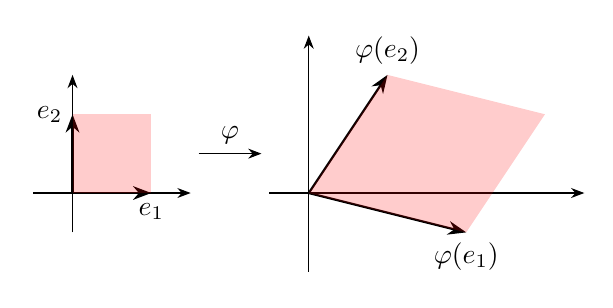
\begin{tikzpicture}[>=Stealth, scale=1]
        \draw[->] (-0.5, 0) -- (1.5, 0);
        \draw[->] (0, -0.5) -- (0, 1.5);
        \draw[thick, ->] (0, 0) -- (1, 0) node[below]{$e_1$};
        \draw[thick, ->] (0, 0) -- (0, 1) node[left]{$e_2$};
        \fill[red, opacity=0.2] (0, 0) -- (1, 0) -- (1, 1) -- (0, 1);
        \begin{scope}[shift={(3, 0)}]
            \draw[->] (-.5, 0) -- (3.5, 0);
            \draw[->] (0, -1) -- (0, 2);
            \draw[thick, ->] (0, 0) -- (2, -.5)
                node[below]{$\varphi(e_1)$};
            \draw[thick, ->] (0, 0) -- (1, 1.5)
                node[above]{$\varphi(e_2)$};
            \fill[red, opacity=0.2] (0, 0) -- (2, -.5)
                -- (3, 1) -- (1, 1.5);
        \end{scope}
        \draw[->] (1.6, 0.5) -- node[above]{$\varphi$}
             (2.4, 0.5);
    \end{tikzpicture}
\end{figure}

但是上面这两条看起来截然不同的路线有什么关系呢?不妨这样想:
\begin{itemize}
    \item 当体积的倍数等于 $0$ 时,这说明原来的空间必然被降维了,这需要通过压缩某个维度来实现,这个维度的所有向量都被压缩到 $0$ 自然就说明了线性方程的重根,也就说明了映射的不可逆;
    \item 反过来当重根存在时,重根这个方向的所有向量都会被映射到 $0$,所以体积会被压缩到 $0$,变化的倍数也变成了 $0$,在这个意义下线性映射的不可逆和 $1/0$ 不存在本质上是一样的.
\end{itemize}

作为判别式,它为我们提供了方便的计算方法:行列式来源于线性方程组,而线性方程组的经典解法就是高斯消元,由此我们可以通过高斯消元得到行列式最方便的计算方法,并在高斯消元的过程中提取出行列式的显式表达式,它构成了按照行或列展开行列式的基础数百年前的数学家们正是在高斯消元中找规律并初次提出了行列式. 同时由于线性方程的解在行变换下不变,反映重根情况的判别式自然具有一些对应的性质,我们可以借助行变换下的若干不变性来定义行列式.

作为体积的变化,它为我们提供了良好的不变性,例如,体积的变化比例自然不会随着基的选取而变化,所以后面可以得出相似变换不改变行列式的结论. 正如我们小学学过的平行四边形面积等于底乘高,将一条边在自身的方向上平移不改变平行四边形的面积,这里的拓展便是列倍加下的不变性,从而也可以用列变换下的若干不变性来定义行列式. 进一步地,Cramer法则也具有很好的几何解释(实质上可以理解为知道面积和底边长的情况下求高)

总的来讲,按行看去是代数,行列式是方程根的判据,反映了重根和可逆性. 按列看去是几何,方程是体积变化的情况,而后会成为特征值的重要研究工具. 从分析学的看来,它在多元微积分的换元中起到了重要的作用. 从组合学看来,行列式按元素表达式的推导也是一种对组合数学的具体应用.

\subsection{从判别式到公理化定义}

为了给出线性方程组的判别式,一个很直接的方法便是直接做高斯消元,对于一个矩阵
\[
A = \begin{pmatrix}
    a_{11} & a_{12} & \cdots & a_{1n} \\
    a_{21} & a_{22} & \cdots & a_{2n} \\
    \vdots & \vdots & \ddots & \vdots \\
    a_{n1} & a_{n2} & \cdots & a_{nn}
\end{pmatrix}
\]
假设消元的过程中没有进行行交换,那么我们可以得到一个上三角矩阵,其主元分别为
\[
\begin{pmatrix}
    a_{11}' & a_{12}' & \cdots & a_{1n}' \\
            & a_{22}' & \cdots & a_{2n}' \\
            &         & \ddots & \vdots  \\
            &         &        & a_{nn}'
\end{pmatrix}
\]
即 $a_{ij}$ 经过 $k$ 次消元后的结果为 $a_{ij}^{(k)}$,那么由于第 $i$ 行需要进行 $i-1$ 次消元,我们有 $a_{ij}' = a_{ij}^{(i-1)}$,于是我们有
\begin{align*}
    a_{22}' = a_{22}^{(1)} &= a_{22} - \frac{a_{21}}{a_{11}}a_{12} = \frac{a_{11}a_{22}-a_{22}a_{21}}{a_{11}} \\
    a_{23}' = a_{23}^{(1)} &= a_{23} - \frac{a_{21}}{a_{11}}a_{13} = \frac{a_{11}a_{23}-a_{21}a_{13}}{a_{11}} \\
     a_{32}^{(2)} &= a_{32} - \frac{a_{31}}{a_{11}}a_{12} = \frac{a_{11}a_{32}-a_{31}a_{12}}{a_{11}} \\
     a_{33}^{(2)} &= a_{33} - \frac{a_{31}}{a_{11}}a_{13} = \frac{a_{11}a_{33}-a_{31}a_{13}}{a_{11}}
\end{align*}
更进一步地我们有
\begin{align*}
    a_{33}' &= a_{33}^{(2)} = a_{33}^{(1)} - \frac{a_{32}^{(2)}}{a_{22}'}a_{23}' \\
    &= \frac{a_{11}a_{22}a_{33} + a_{12}a_{23}a_{31}+a_{31}a_{12}a_{23}-a_{11}a_{32}a_{23}-a_{12}a_{21}a_{33} - a_{13}a_{22}a_{31}}{a_{11}a_{22}- a_{12}a_{21}}
\end{align*}
如此消元下去我们便会发现,$a_{ij}'$ 的分子和分母都是关于这些系数的多项式,且 $a_{k+1,k+1}$ 的分子恰好为 $a_{kk}$ 的分母,即结果具有形式(为了方便我们令 $\Delta_0 = 1$,这里略过对 $a_{kk}'$ 具有如下形式这一结论的证明)
\[
a_{11}' = \frac{\Delta_1}{\Delta_0},\quad a_{22}' = \frac{\Delta_2}{\Delta_1},\quad \cdots,\quad a_{nn}' = \frac{\Delta_n}{\Delta_{n-1}}
\]
注意到消元的过程中,$\Delta_k$ 是否为 $0$ 会决定消元是否能够继续进行,所以它们有着重要的意义,这时我们称 $\Delta_k$ 为 $A$ 的 $k$ 阶\term{主子式},而 $\Delta_n$ 便是 $A$ 的\term{行列式},记作 $\det A$. 这便是从消元引出的定义,它是一个数,是一个矩阵的一个重要的性质,主子式是否为 $0$ 决定了消元是否能够继续进行. 如果探究多项式的形式我们就可以得到一些重要性质:在每行乘以常数结果会对应地乘以这个常数,交换两行会改变符号,两行相加不会改变行列式的值,且单位矩阵的行列式为 $1$. 然而这个多项式的形式并不是很容易理解,所以我们引入了行列式的公理化定义.

\subsection{从体积变化到公理化定义}

另一方面,我们可以从体积变化的角度来定义行列式. 为了方便讨论,我们先考虑二维空间中的情况. 或许最重要的形式就是由于两个映射的复合导致的体积变化是两次体积变化的乘积,因此它是一个函数使得 $f(AB) = f(A)f(B)$. 这会导致对角矩阵
\[\diag(\lambda_1, \lambda_2, \cdots, \lambda_n) = \lambda_1\lambda_2\cdots\lambda_n\]
因为这一变换可以理解为对每个坐标轴对应的缩放. 一些技巧可以证明行变换矩阵的行列式为 $1$(但是我们这里略去这一证明),行列式的计算方式亦然可以由此导出.

由于行列式有众多等价的定义方式,下面我们选取较为简洁的一种,即使用若干条公理定义行列式. 在这种定义下,我们可以很容易地推导出行列式的一些基本性质,然后引入逆序数定义,最后再引入判别式的定义,这样的顺序更加符合我们的思路,也更加便于理解.


\section{行列式的公理化定义}

\subsection{公理化定义}

\begin{definition}{行列式}{公理化定义}
    数域$\mathbf{F}$上的一个$n$阶\term{行列式}是取值于$\mathbf{F}$的$n$个$n$维向量$\alpha_1,\alpha_2,\ldots,\alpha_n \in \mathbf{F}^n$的一个函数,且$\forall \alpha_i,\beta_i \in \mathbf{F}^n$和$\forall \lambda \in \mathbf{F}$,满足下列规则:
    \begin{enumerate}
        \item \label{item:13:齐性}
              (齐性) $D(\alpha_1,\ldots,\lambda\alpha_i,\ldots,\alpha_n)=\lambda D(\alpha_1,\ldots,\alpha_i,\ldots,\alpha_n)$;

        \item \label{item:13:加性}
              (加性,与 \ref*{item:13:齐性} 合称线性性) \\
              $D(\alpha_1,\ldots,\alpha_i+\beta_i,\ldots,\alpha_n)=D(\alpha_1,\ldots,\alpha_i,\ldots,\alpha_n)+D(\alpha_1,\ldots,\beta_i,\ldots,\alpha_n)$;

        \item \label{item:13:反对称性}
              (反对称性) $D(\alpha_1,\ldots,\alpha_i,\ldots,\alpha_j,\ldots,\alpha_n)=-D(\alpha_1,\ldots,\alpha_j,\ldots,\alpha_i,\ldots,\alpha_n)$;

        \item \label{item:13:规范性}
              (规范性) $D(e_1,e_2,\ldots,e_n)=1$.
    \end{enumerate}
\end{definition}

在公理化定义中,我们将行列式定义为一个满足特定的运算性质的从列向量组合到数的函数. 需要注意的是,行列式除了上述记法外,如果设矩阵 $A = (\alpha_1,\ldots,\alpha_n)$,那么行列式 $D(\alpha_1,\ldots,\alpha_n)$ 也可以记为 $|A|$.

不难看出公理化定义可以形象地理解为对 $n$ 维空间中体积的定义,因此与此前引入的几何直观一致. 对几何意义感兴趣的同学可以参考 \href{https://b23.tv/BV1ys411472E}{3b1b《线性代数的本质》系列视频}相关内容.

\subsection{行列式的简单性质}

下面的例子给出了从公理化定义出发证明的行列式的一些简单性质:

\begin{example}{}{公理化定义}
    使用\autoref{def:公理化定义} 验证下述命题的正确性:
    \begin{enumerate}
        \item 若行列式有一列为零向量,则行列式的值等于0.

        \item 若行列式有两列元素相同,则行列式的值等于0.

        \item 若行列式有两列元素成比例,则行列式的值等于0.

        \item 对行列式做倍加列变换,行列式的值不变.

        \item \label{item:13:公理化定义导出性质:5}
            若$\alpha_1,\alpha_2,\ldots,\alpha_n$线性相关,则$D(\alpha_1,\alpha_2,\ldots,\alpha_n)=0$.
    \end{enumerate}
\end{example}

\begin{proof}
    \begin{enumerate}
        \item 由于行列式满足\autoref{def:公理化定义} 的\ref*{item:13:齐性},设行列式第$i$列为零向量,因此
              \begin{align*}
                  D(\alpha_1,\ldots,0,\ldots,\alpha_n) & =D(\alpha_1,\ldots,0\cdot\alpha_i,\ldots,\alpha_n)  \\
                                                       & =0\cdot D(\alpha_1,\ldots,\alpha_i,\ldots,\alpha_n) \\
                                                       & =0
              \end{align*}

        \item 由于行列式满足\autoref{def:公理化定义} 的\ref*{item:13:反对称性},设行列式第$i$列和第$j$列元素相同,因此
              \begin{align*}
                  D(\alpha_1,\ldots,\alpha_i,\ldots,\alpha_j,\ldots,\alpha_n) & =D(\alpha_1,\ldots,\alpha_j,\ldots,\alpha_i,\ldots,\alpha_n)  \\
                                                                              & =-D(\alpha_1,\ldots,\alpha_i,\ldots,\alpha_j,\ldots,\alpha_n)
              \end{align*}
              从而$D(\alpha_1,\ldots,\alpha_i,\ldots,\alpha_j,\ldots,\alpha_n)=0$.

        \item 由于行列式满足\autoref{def:公理化定义} 的\ref*{item:13:齐性},设行列式第$i$列和第$j$列元素成比例,$\alpha_i=k\alpha_j$,因此
              \begin{align*}
                  D(\alpha_1,\ldots,\alpha_i,\ldots,\alpha_j,\ldots,\alpha_n)
                   & =D(\alpha_1,\ldots,k\alpha_j,\ldots,\alpha_j,\ldots,\alpha_n) \\
                   & =kD(\alpha_1,\ldots,\alpha_j,\ldots,\alpha_j,\ldots,\alpha_n) \\
                   & =0.
              \end{align*}
              其中最后一个等号用到了本例的第二条结论.

        \item 事实上,根据\autoref{def:公理化定义} 的\ref*{item:13:加性} 以及本例第3条结论,我们可以得到
              \begin{align*}
                  D(\alpha_1,\ldots,\alpha_i+k\alpha_j,\ldots,\alpha_j,\ldots,\alpha_n)
                   & =D(\alpha_1,\ldots,\alpha_i,\ldots,\alpha_j,\ldots,\alpha_n)   \\&+D(\alpha_1,\ldots,k\alpha_j,\ldots,\alpha_j,\ldots,\alpha_n) \\
                   & =D(\alpha_1,\ldots,\alpha_i,\ldots,\alpha_j,\ldots,\alpha_n)+0 \\
                   & =D(\alpha_1,\ldots,\alpha_i,\ldots,\alpha_j,\ldots,\alpha_n).
              \end{align*}

        \item 设$\alpha_1,\alpha_2,\ldots,\alpha_n$线性相关,因此存在不全为0的数$k_1,k_2,\ldots,k_n$使得$k_1\alpha_1+k_2\alpha_2+\cdots+k_n\alpha_n=0$,不妨设$k_1 \neq 0$,因此
              \[\alpha_1=-\frac{k_2}{k_1}\alpha_2-\frac{k_3}{k_1}\alpha_3-\cdots-\frac{k_n}{k_1}\alpha_n,\]
              因此
              \begin{align*}
                  D(\alpha_1,\alpha_2,\ldots,\alpha_n) & =D(-\frac{k_2}{k_1}\alpha_2-\frac{k_3}{k_1}\alpha_3-\cdots-\frac{k_n}{k_1}\alpha_n,\alpha_2,\ldots,\alpha_n)     \\
                                                       & =-\frac{k_2}{k_1}D(\alpha_2,\alpha_2,\ldots,\alpha_n)-\cdots-\frac{k_n}{k_1}D(\alpha_n,\alpha_2,\ldots,\alpha_n) \\
                                                       & =0.
              \end{align*}
    \end{enumerate}
\end{proof}

请分别从公理化定义和行列式几何意义出发理解上述五条性质.

使用公理化定义可以对一些简单的行列式进行计算:

\begin{example}{}{从公理化定义出发计算行列式}
    计算行列式 $D = \begin{vmatrix}
        1 & 2 \\
        2 & 3
    \end{vmatrix}$.
\end{example}

\begin{solution}
    设 $\alpha_1 = (1, 2)$, $\alpha_2 = (2, 3)$,将行列式 $D$ 写成向量形式并用公理化定义展开可得:

    \begin{align*}
        D &= D(\alpha_1, \alpha_2) = D(e_1 + 2e_2, 2e_1 + 3e_2) \\
          &= D(e_1, 2e_1 + 3e_2) + 2 D(e_2, 2e_1 + 3e_2) \\
          &= 2D(e_1, e_1) + 3D(e_1, e_2) + 4D(e_2, e_1) + 6D(e_2, e_2) \\
          &= 3 - 4 = -1.
    \end{align*}
\end{solution}

\begin{example}{}{公理化定义2}
    设向量$\alpha_1,\alpha_2,\beta_1,\beta_2$为三维列向量,又$A=(\alpha_1,\alpha_2,\beta_1),B=(\alpha_1,\alpha_2,\beta_2)$,且$|A|=3$,$|B|=2$,求$|2A+3B|$.
\end{example}

\begin{solution}
    $2A+3B=(2\alpha_1+3\alpha_1,2\alpha_2+3\alpha_2,2\beta_1+3\beta_2)=(5\alpha_1,5\alpha_2,2\beta_1+3\beta_2)$,因此
    \begin{align*}
        |2A+3B| & =|5\alpha_1,5\alpha_2,2\beta_1+3\beta_2|                       \\
                & =25|\alpha_1,\alpha_2,2\beta_1+3\beta_2|                       \\
                & =25(2|\alpha_1,\alpha_2,\beta_1|+3|\alpha_1,\alpha_2,\beta_2|) \\
                & =25(2|A|+3|B|)=300.                                            \\
    \end{align*}
\end{solution}

上(下)三角行列式是一类非常重要的特殊行列式,在行列式有关的计算与证明中经常出现,下面我们通过行列式的公理化定义来证明上(下)三角行列式的一个重要性质:

\begin{example}{上三角矩阵的行列式}{}
    证明上三角矩阵的行列式的值等于其主对角线元素之积,即证明对任意矩阵

    \[
        A = \begin{pmatrix}
            a_{11} & a_{12} & \cdots & a_{1n} \\
            0      & a_{22} & \cdots & a_{2n} \\
            \vdots & \vdots & \ddots & \vdots \\
            0      & 0      & \cdots & a_{nn}
        \end{pmatrix},
    \]

    有 $|A| = \prod_{i=1}^n a_{ii}$.
\end{example}

\begin{proof}
    设 $A$ 为上三角矩阵,其对角线元素为 $a_{11}, a_{22}, \ldots, a_{nn}$,若 $\exists a_{ii} = 0$,则 $A$ 的列向量线性相关,$|A| = 0$;反之,若 $a_{ii} \neq 0, \enspace i=1,2,\ldots,n$,则对 $A$ 作倍加列变换可将 $A$ 化为对角矩阵 $\mathrm{diag}(a_{11},a_{22},\ldots,a_{nn})$,故 $|A| = \prod_{i=1}^n a_{ii}$.
\end{proof}

公理化定义告诉了我们行列式满足的几条基本性质,并且清晰地反映了行列式的几何意义. 然而,行列式作为一种工具,势必需要一种比公理化定义更为直观的计算方法,换句话说,我们希望找到 $|A|$ 关于 $a_{ij}$ 的关系式。

\section{第一条路:行列式的逆序数定义}

在\autoref{ex:从公理化定义出发计算行列式} 中我们用到了硬拆法:把每个列向量拆成单位正交基的线性组合,然后拆成 $2^n$ 个可以使用公理化定义求解的行列式. 下面我们把这种方法规范化:给定一个行列式

\[|A| = \begin{vmatrix}
        a_{11} & a_{12} & \cdots & a_{1n} \\
        a_{21} & a_{22} & \cdots & a_{2n} \\
        \vdots & \vdots & \ddots & \vdots \\
        a_{n1} & a_{n2} & \cdots & a_{nn}
    \end{vmatrix},\]

为了叙述方便,我们记 $A = (\alpha_1,\ldots,\alpha_n)$,并记 $e_i$ 为 $n$ 维单位向量,即 $e_i = (0,\ldots,1,\ldots,0)$,其中 $1$ 在第 $i$ 个位置. 这样,行列式的第 $j$ 列就可以表达为

\[\alpha_j = a_{1j}e_1 + a_{2j}e_2 + \cdots + a_{nj}e_n = \sum_{i=1}^{n}a_{ij}e_i.\]

于是,根据行列式公理化定义\autoref{def:公理化定义} 的线性性质,我们有

\begin{align*}
    |A| & = |\alpha_1,\alpha_2,\ldots,\alpha_n| = |\sum\limits_{i=1}^{n}a_{i1}e_i,\alpha_2,\ldots,\alpha_n| \\
        & = \sum\limits_{i=1}^{n}a_{i1}|e_i,\alpha_2,\ldots,\alpha_n|.
\end{align*}

对行列式 $|e_i,\alpha_2,\ldots,\alpha_n|$ 继续展开,由 $\alpha_2 = \sum\limits_{j=1}^{n}a_{j2}e_j$,我们有

\[|e_i,\alpha_2,\ldots,\alpha_n| = \sum\limits_{j=1}^{n}a_{j2}|e_i,e_j,\alpha_3,\ldots,\alpha_n|.\]

于是 $|A| = \sum\limits_{i=1}^{n}\sum\limits_{j=1}^{n}a_{i1}a_{j2}|e_i,e_j,\alpha_3,\ldots,\alpha_n|$. 不断展开,我们最终得到

\[|A| = \sum\limits_{k_1,k_2,\ldots,k_n} a_{k_11}a_{k_22}\cdots a_{k_nn}|e_{k_1},e_{k_2},\ldots,e_{k_n}|.\]

以上为硬拆法的基本流程. 注意行列式 $|e_{k_1},e_{k_2},\ldots,e_{k_n}|$ 在某对 $k_i,k_j$ 重复时的值为 $0$,所以在不为 $0$ 的项中,$(k_1,k_2,\ldots,k_n)$ 必定是 $(1,2,\ldots,n)$ 的一个全排列,即在 $k_1,k_2,\ldots,k_n$ 中,$1,2,\ldots,n$ 中每个数都出现且仅出现一次. 设 $S_n$ 为 $1,2,\ldots,n$ 所有全排列构成的集合,那么 $S_n$ 的元素个数为 $n!$.

进一步地,当 $(k_1,k_2,\ldots,k_n) \in S_n$ 时,行列式 $|e_{k_1},e_{k_2},\ldots,e_{k_n}|$ 的每一行、每一列都有且只有一个元素等于 $1$,其余元素都等于 $0$,因此 $|e_{k_1},e_{k_2},\ldots,e_{k_n}| = \pm 1$,因此 $|A|$ 的展开式一共有 $n!$ 项,可以表达为

\[|A| = \sum\limits_{k_1,k_2,\ldots,k_n} (-1)^\varepsilon a_{k_11}a_{k_22}\cdots a_{k_nn}.\]

下面我们需要确定 $\varepsilon$ 的取值,可以肯定它是一个关于排列 $(k_1, k_2, \ldots, k_n)$ 的一个函数,下面我们引入逆序数的概念来帮助我们确定 $\varepsilon$ 的值:

\begin{definition}{逆序数}{}
    设 $k_1,k_2,\ldots,k_n \in S_n$,如果 $i < j$ 且 $k_i > k_j$,则称 $k_i,k_j$ 是这个排列的一个\term{逆序对}\index{nixudui@逆序对},排序中所有逆序对的总数称为这个排列的\term{逆序数}\index{nixushu@逆序数},记作 $\tau(k_1,k_2,\ldots,k_n)$.
\end{definition}
逆序数的定义是非常易懂的,就是位置在前但数值更大的情况出现的次数. 直观上来看,逆序数衡量了与\term{常序排列} $(1,2,\ldots,n)$ 之间的距离,逆序数越大,排列与常序排列的差距越大. 逆序数的求法也非常简单:设排列为 $(k_1,k_2,\ldots,k_n)$,那么我们先看 $k_1$ 后面有多少个数比 $k_1$ 小,然后看 $k_2$ 后面有多少个数比 $k_2$ 小,以此类推,最后将所有这些数相加即可. 我们来看一个简单的例子:

\begin{example}{}{}
    求排列 $(3,1,4,2)$ 的逆序数.
\end{example}

\begin{solution}
    我们可以直接计算:$3$ 后面有 $2$ 个数比 $3$ 小,$1$ 后面没有数比 $1$ 小,$4$ 后面有 $1$ 个数比 $4$ 小,$2$ 后面没有数比 $2$ 小,因此逆序数为 $2+0+1+0=3$.
\end{solution}

基于逆序数的定义,我们可以将排列做一个简单的分类:

\begin{definition}{奇排列和偶排列}{}
    如果一个排列的逆序数是偶数(包括零),则称这个排列是\term{偶排列}\index{oupailie@偶排列};如果一个排列的逆序数是奇数,则称这个排列是\term{奇排列}\index{jipailie@奇排列}.
\end{definition}

不难证明奇偶排列有如下简单的性质:
\begin{example}{奇偶排列的性质}{}
    \begin{enumerate}
        \item 设 $(k_1,k_2,\ldots,k_n) \in S_n$,若将 $k_i$ 与 $k_j$ 交换,其余数不动,那么排列的奇偶性会改变;
        \item 设 $n \geqslant 2$,则 $S_n$ 中奇排列和偶排列的个数相等.
    \end{enumerate}
\end{example}

\begin{proof}
    \begin{enumerate}
        \item 首先我们考虑相邻两个数的对换. 若 $k_i > k_{i+1}$,则对换后逆序数会减少 $1$,因此奇偶性会改变;若 $k_i < k_{i+1}$,则对换后逆序数会增加 $1$,奇偶性也会改变. 对于一般情形,$k_i$ 和 $k_j$ 的对换可以通过多次相邻两个数的对换来实现:不妨设 $i < j$,那么我们可以先将 $k_i$ 与 $k_{i+1}$ 对换,然后与 $k_{i+2}$ 对换,以此类推,最后与 $k_j$ 对换,这样就可以将 $k_i$ 和 $k_j$ 对换(一共对换了 $j-i$ 次);接下来还需要将 $k_j$ 与 $k_{j-1}$ 对换,然后与 $k_{j-2}$ 对换,以此类推,最后与 $k_{i+1}$ 对换(一共对换了 $j-i-1$ 次),这样就可以将 $k_j$ 和 $k_i$ 对换. 因此,总的相邻对换次数为 $j-i+j-i-1=2(j-i)-1$,奇偶性会改变.
        \item 设 $S_n$ 中奇排列有 $p$ 个,偶排列有 $q$ 个,因为 $n \geqslant 2$,故可以将每个奇排列的头两个数对换一下,则所有的奇排列都变成了互不相同的偶排列,故 $p \leqslant q$;同理,可以将每个偶排列的头两个数对换一下,所有的偶排列都变成了互不相同的奇排列,故 $q \leqslant p$,因此 $p = q$.
    \end{enumerate}
\end{proof}

讨论到此,我们终于可以给出逆序数与行列式展开中每项的符号之间的联系:

\begin{theorem}{}{逆序数与幂次的关系}
    设 $(k_1,k_2,\ldots,k_n) \in S_n$,则通过 $\tau(k_1,k_2,\ldots,k_n)$ 次相邻对换可以将 $(k_1,k_2,\ldots,k_n)$ 变为 $(1,2,\ldots,n)$,因此 $\varepsilon = \tau(k_1,k_2,\ldots,k_n)$.
\end{theorem}

\begin{proof}
    对 $n$ 进行归纳. $n=1$ 时结论显然成立,设对 $1,2,\ldots,n-1$ 的任一排列结论成立,我们来证明 $n$ 的情形. 设 $n$ 在排列 $(k_1,\ldots,k_n)$ 的第 $i$ 位,即 $k_i = n$,$n$ 贡献的逆序数为 $m_i = n - i$. 将 $k_i$ 与 $k_{i+1}$ 对换,再与 $k_{i+2}$ 对换,以此类推,最后与 $k_n$ 对换,这样 $n$ 就到了第 $n$ 位. 注意到

    \[ \tau(k_1,\ldots,k_n) = \tau(k_1,\ldots,k_{i-1},k_{i+1},\ldots,n) + m_i,\]

    且 $(k_1,\ldots,k_{i-1},k_{i+1},\ldots,n) \in S_{n-1}$,由归纳假设知 $(k_1,\ldots,k_{i-1},k_{i+1},\ldots,n)$ 经过 $\tau(k_1,\ldots,k_{i-1},k_{i+1},\ldots,n)$ 次相邻对换可以变为 $(1,2,\ldots,n-1)$,结合上面的讨论可知 $(k_1,\ldots,k_n)$ 经过 $\tau(k_1,\ldots,k_n)$ 次相邻对换可以变为 $(1,2,\ldots,n)$,因此 $\varepsilon = \tau(k_1,\ldots,k_n)$.
\end{proof}

事实上,我们也可以给出\autoref{thm:逆序数与幂次的关系} 的一种更为直观的理解:由公理化定义,我们知道 $\epsilon$ 的取值实质上是将 $|e_{k_1}, e_{k_2}, \ldots, e_{k_n}|$ 通过行列对换得到 $|e_1, e_2, \ldots, e_n|$ 的次数. 令 $k_m = n$ 为 $k_1, k_2, \ldots, k_n$ 中最大的元素,我们先将 $e_{k_m}$ 通过相邻列交换的方式换到最后一列,这个过程中需要交换 $n - m$ 次,而由于 $k_m > k_i, \forall i > m$,故交换的过程中我们``解决''了 $n - m$ 个逆序对,这与交换次数是相同的. 第一轮交换结束后,我们得到了 $|e_{k_1}, e_{k_2}, \ldots, e_{k_{m-1}}, e_{k_n}, e_{k_{m+1}}, \ldots, e_{k_{n-1}, e_{k_m}}$,可以看到第一轮交换并没有``解决''与 $k_m$ 无关的逆序对. 接着我们只需要重复将前 $n-p$ 个向量中下标最大的向量交换到第 $n-p$ 个位置上的操作即可,而上面我们已经说明了操作过程中的交换次数与``解决''的逆序数是相同的. 因此我们可以知道总的交换次数 $\epsilon$ 就是所有``解决''的逆序数个数 $\tau(k_1,k_2,\ldots,k_n)$.

我们由此给出行列式的逆序数定义:

\begin{theorem}{行列式的逆序数定义}{}
    设
    \[|A| = \begin{vmatrix}
            a_{11} & a_{12} & \cdots & a_{1n} \\
            a_{21} & a_{22} & \cdots & a_{2n} \\
            \vdots & \vdots & \ddots & \vdots \\
            a_{n1} & a_{n2} & \cdots & a_{nn}
        \end{vmatrix},\]
    则 $|A| = \sum\limits_{(k_1,k_2,\ldots,k_n) \in S_n} (-1)^{\tau(k_1,k_2,\ldots,k_n)}a_{k_11}a_{k_22}\cdots a_{k_nn}$.
\end{theorem}

下面我们给出逆序数定义与公理化定义的等价性. 上文已经说明从公理化定义得到逆序数定义的过程,因此我们只需说明如何从逆序数定义得到公理化定义即可:

\begin{proof}
    \begin{enumerate}
        \item (线性性)使用逆序数定义对行列式进行展开:
            \begin{align*}
                & D(\alpha_1, \ldots , \lambda\alpha_i + \mu\beta_i, \ldots, \alpha_n) \\
                ={} & \sum_{(k_1, k_2, \ldots, k_n) \in S_n} (-1)^{\varepsilon} a_{k_1 1} \cdots a_{k_{i-1},i-1} (\lambda a_{k_i i} + \mu b_{k_i i}) a_{k_{i+1},i+1} \cdots a_{k_n n} \\
                ={} & \lambda \left(\sum_{(k_1, k_2, \ldots, k_n) \in S_n} (-1)^{\varepsilon} a_{k_1 1} \cdots a_{k_{i-1},i-1} a_{k_i i} a_{k_{i+1},i+1} \cdots a_{k_n n} \right) + \\
                    {} & \mu \left(\sum_{(k_1, k_2, \ldots, k_n) \in S_n} (-1)^{\varepsilon} a_{k_1 1} \cdots a_{k_{i-1},i-1} b_{k_i i} \cdots a_{k_n n}\right) \\
                ={} & \lambda D(\alpha_1, \ldots, \alpha_i, \ldots, \alpha_n) + \mu D(\alpha_1, \ldots, \beta_i, \ldots, \alpha_n),
            \end{align*}
            其中 $\varepsilon = \tau(k_1, k_2, \ldots, k_n)$ 表示排列 $(k_1, k_2, \ldots, k_n)$ 的逆序数.

        \item (反对称性)对于 $D(\alpha_1, \ldots, \alpha_i, \ldots, \alpha_j, \ldots, \alpha_n)$ 逆序数定义展开式中的任意一项
            \[
                (-1)^{\tau(k_1, \ldots, k_i, \ldots, k_j, \ldots, k_n)} a_{k_1 1} \cdots a_{k_i i} \cdots a_{k_j j} \cdots a_{k_n n},
            \]

            其可以对应 $D(\alpha_1, \ldots, \alpha_j, \ldots, \alpha_i, \ldots, \alpha_n)$ 逆序数定义展开式中的一项
            \[
                (-1)^{\tau(k_1, \ldots, k_j, \ldots, k_i, \ldots, k_n)} a_{k_1 1} \cdots a_{k_j j} \cdots a_{k_i i} \cdots a_{k_n n}.
            \]

            而排列 $(k_1, \ldots, k_i, \ldots, k_j, \ldots, k_n)$ 与 $(k_1, \ldots, k_j, \ldots, k_i, \ldots, k_n)$ 的奇偶性必定相反,故以上两个对应项为相反数,因此有
            \[
                D(\alpha_1, \ldots, \alpha_j, \ldots, \alpha_i, \ldots, \alpha_n) = -D(\alpha_1, \ldots, \alpha_i, \ldots, \alpha_j, \ldots, \alpha_n).
            \]

        \item (规范性)$E_n$ 的逆序数定义展开式中只有一项
            \[
                (-1)^{\tau(1, 2, \ldots, n)} a_{11} a_{22} \cdots a_{nn}
            \]
            不为零,故 $|E_n| = 1$.
    \end{enumerate}
\end{proof}

下面的例子会让我们更进一步地理解逆序数定义中``排列''的含义:
\begin{example}{}{}
    设
    \[f(x)=\begin{vmatrix}
            x-a_{11} & -a_{12}  & \cdots & -a_{1n}  \\
            -a_{21}  & x-a_{22} & \cdots & -a_{2n}  \\
            \vdots   & \vdots   & \ddots & \vdots   \\
            -a_{n1}  & -a_{n2}  & \cdots & x-a_{nn}
        \end{vmatrix},\]
    其中$x$是未知数,$a_{ij}$是常数,证明:$f(x)$是一个最高次项系数为1的$n$次多项式,且其$n-1$次项的系数等于$-(a_{11}+\cdots+a_{nn})$.
\end{example}

\begin{proof}
    根据逆序数定义,我们知道 $f(x)$ 的最高次项出现在展开式中的单项 $(x-a_{11})(x-a_{22})\cdots(x-a_{nn})$ 中,且展开式中的其他单项作为 $x$ 的多项式的次数必定小于等于 $n-2$(因为我们要求 $(k_1,\ldots,k_n)$ 是全排列). 因此 $f(x)$ 是一个最高次项系数为 $1$ 的 $n$ 次多项式,且其 $n-1$ 次项的系数只能来源于 $(x-a_{11})(x-a_{22})\cdots(x-a_{nn})$,故等于 $-(a_{11}+\cdots+a_{nn})$.
\end{proof}

\section{第二条路:行列式的递归式定义}

找到了行列式的 ``通项公式'',下面我们来推导行列式的 ``递推公式'',即其递归式定义. 首先我们需要引入余子式和代数余子式的概念:

\begin{definition}{}{余子式}
    在$n$阶行列式$D=|a_{ij}|_{n \times n}$中,去掉元素$a_{ij}$所在的第$i$行和第$j$列的所有元素而得到的$n-1$阶行列式称为元素$a_{ij}$的\term{余子式}\index{yuzishi@余子式 (minor)},记作$M_{ij}$,并把数$A_{ij}=(-1)^{i+j}M_{ij}$称为元素$a_{ij}$的\term{代数余子式}\index{yuzishi!daishu@代数余子式 (cofactor)}.
\end{definition}

注意,虽然余子式和代数余子式在名称中含有式,但实际上他们是一个值. 实际上行列式也称为``式'',但这些``式''只是形状上有个形式,实际上只是一个值.
\begin{example}{}{余子式}
    根据\autoref{def:余子式} 计算行列式$\begin{vmatrix}
            2  & 1 & 3  \\
            -1 & 0 & 2  \\
            1  & 5 & -2
        \end{vmatrix}$每个元素的余子式和代数余子式.
\end{example}

\begin{solution}
    我们只举一个例子,第二行第一列元素$-1$的余子式和代数余子式. 根据定义,它的余子式是去掉第二行和第一列所有元素剩余的二阶行列式
    \[\begin{vmatrix}
            1 & 3  \\
            5 & -2
        \end{vmatrix}=-17,\]
    因此它的代数余子式是$A_{21}=(-1)^{2+1}(-17)=17$. 读者可以自行计算其他元素的余子式和代数余子式.
\end{solution}

接下来我们便可以给出递归式定义:
\begin{definition}{}{递归式定义}
    设$D=|a_{ij}|_{n \times n}$,则
    \begin{align}
        \label{eq:13:递归式定义1}
        D=\sum_{k=1}^{n}a_{kj}A_{kj}=a_{1j}A_{1j}+a_{2j}A_{2j}+\cdots+a_{nj}A_{nj} & \qquad j=1,2,\ldots,n \\
        \label{eq:13:递归式定义2}
        D=\sum_{k=1}^{n}a_{ik}A_{ik}=a_{i1}A_{i1}+a_{i2}A_{i2}+\cdots+a_{in}A_{in} & \qquad i=1,2,\ldots,n
    \end{align}
\end{definition}
其中$A_{ij}$即为\autoref{def:余子式} 给出的代数余子式,\autoref{eq:13:递归式定义1} 称为$D$对第$j$列的展开式,\autoref{eq:13:递归式定义2} 称为$D$对第$i$行的展开式. 事实上,这一定义被称为递归式定义的原因是显然的(如果在程序设计课程中已经学习过递归的概念),它使用$n-1$阶行列式定义$n$阶行列式,因此我们对任意$n$阶行列式都可以递归展开到1阶,从而得到最终行列式计算结果.

除此之外,我们需要强调的是,这里的递归式定义能称之为定义,必须要使得其与之前的公理化定义不冲突. 事实上二者等价的证明都是技术性的,从公理化定义推出递归式定义需要利用公理化定义将原行列式进行拆分与变形,反过来我们只需要对公理化定义中每个性质利用递归式定义逐个展开验算即可:

\begin{proof}
    \begin{enumerate}
        \item 公理化定义 $\implies$ 递归式定义:

            先证明一个引理:设 $A=(a_{ij})_{n \times n}$ 中 $a_{in}=0,\enspace i = 1, 2, \ldots, n-1$,则 $|A| = a_{nn} M_{nn} = a_{nn} A_{nn}$.

            将 $A$ 分块表示为
            \[
                A = \begin{pmatrix}
                    A_1             & \mathbf{0} \\
                    \mathbf{\alpha} & a_{nn}
                \end{pmatrix},
            \]

            其中 $|A_1| = M_{nn} = A_{nn}$. 若 $a_{nn} = 0$,则 $A$ 不可逆,$|A| = 0$,引理成立;若 $A_1$ 不可逆,则 $r(A) \leqslant r(A_1) + 1 < n$,故 $A$ 不可逆,$|A| = 0$,引理亦成立;若 $a_{nn} \neq 0$ 且 $A_1$ 可逆,则对 $A$ 作倍加列变换,有
            \[
                |A| = \begin{vmatrix}
                    A_1             & \mathbf{0} \\
                    \mathbf{0}      & a_{nn}
                \end{vmatrix}.
            \]

            再对 $A$ 作倍加行变换,将 $A_1$ 化为上三角矩阵 $B_1$,且有 $|B_1| = |A_1| = M_{nn}$,此时有
            \[
                |A| = \begin{vmatrix}
                    B_1             & \mathbf{0} \\
                    \mathbf{0}      & a_{nn}
                \end{vmatrix} = a_{nn} B_1 = a_{nn} M_{nn}.
            \]

            上式成立是因为上三角矩阵的行列式等于其对角线元素之积.

            下面我们来通过公理化定义推出递归式定义. 我们先推导行列式 $D=|a_{ij}|_{n \times n}$ 对第 $j$ 列元素的展开式:

            令 $\alpha_j$ 为 $A$ 中第 $j$ 列的元素,则由公理化定义可得
            \begin{align*}
                D &= D(\alpha_1, \alpha_2, \ldots, \alpha_j, \ldots, \alpha_n) \\
                  &= D(\alpha_1, \alpha_2, \ldots, \sum_{i=1}^n a_{ij} e_i, \ldots, \alpha_n) \\
                  &= \sum_{i=1}^n D(\alpha_1, \alpha_2, \ldots, a_{ij} e_i, \ldots, \alpha_n).
            \end{align*}
            对于上式中的第 $i$ 项 $D_i$,我们将第 $j$ 列依次与第 $j+1, j+2, \ldots, n$ 列对换,再将第 $i$ 行依次与第 $i+1, i+2, \ldots, n$ 行对换,于是有
            \[
                D_i = (-1)^{2n-i-j} \begin{vmatrix}
                    a_{11}     & \cdots & a_{1, j-1}   & a_{1, j+1}   & \cdots & a_{1n}     & 0      \\
                    \vdots     &        &              &              &        &            & \vdots \\
                    a_{i-1, 1} & \cdots & a_{i-1, j-1} & a_{i-1, j+1} & \cdots & a_{i-1, n} & 0      \\
                    a_{i+1, 1} & \cdots & a_{i+1, j-1} & a_{i+1, j+1} & \cdots & a_{i+1, n} & 0      \\
                    \vdots     &        &              &              &        &            & \vdots \\
                    a_{n1}     & \cdots & a_{n, j-1}   & a_{n, j+1}   & \cdots & a_{nn}     & 0      \\
                    a_{i1}     & \cdots & a_{i, j-1}   & a_{i, j+1}   & \cdots & a_{in}     & a_{ij}
                \end{vmatrix} = \begin{vmatrix}
                    A_1         & 0      \\
                    \alpha_{ij} & a_{ij}
                \end{vmatrix}.
            \]

            根据引理,我们有
            \[
                D_i = (-1)^{2n-i-j} a_{ij} |A_1| = (-1)^{i+j} a_{ij} M_{ij} = a_{ij} A_{ij}.
            \]

            由此可得行列式的递推式定义:
            \[
                D = \sum_{i=1}^n D_i = \sum_{i=1}^n a_{ij} A_{ij}.
            \]

        \item 递归式定义 $\implies$ 公理化定义:
            \begin{enumerate}
                \item (线性性)直接将公理化定义用递归式对第$i$列展开:
                    \begin{align*}
                            & D(\alpha_1,\ldots,\lambda\alpha_{i}+\mu\beta_i,\ldots,\alpha_n)                                      \\
                        ={} & \sum_{k=1}^{n}(\lambda a_{ki}+\mu b_{ki})A_{ki}                                                      \\
                        ={} & \lambda \cdot \sum_{k=1}^{n}a_{ki}A_{ki}+\mu \cdot \sum_{k=1}^{n}b_{ki}A_{ki}                        \\
                        ={} & \lambda D(\alpha_1,\ldots,\alpha_{i},\ldots,\alpha_n)+\mu D(\alpha_1,\ldots,\beta_i,\ldots,\alpha_n),
                    \end{align*}
                    则线性性得证.

                \item (反对称性)使用数学归纳法证明. 显然,$D(\alpha_1,\alpha_2)=-D(\alpha_2,\alpha_1)$,然后做出归纳假设:对于任意正整数$i,j$,$1 \leqslant i, j \leqslant n - 1$且$i \neq j$,有:
                    \[ D(\alpha_1,\ldots,\alpha_i,\ldots,\alpha_j,\ldots,\alpha_{n-1})=-D(\alpha_1,\ldots,\alpha_j,\ldots,\alpha_i,\ldots,\alpha_{n-1}). \]
                    由此做出递推,对交换前后的行列式的首行做展开:
                    \begin{gather*}
                        D(\alpha_1,\ldots,\alpha_{i},\ldots,\alpha_{j},\ldots,\alpha_n)
                         =\sum_{k=1}^{n}a_{1k}A_{1k},   \\
                        D(\alpha_1,\ldots,\alpha_{j},\ldots,\alpha_{i},\ldots,\alpha_n)
                         =\sum_{k=1}^{n}a'_{1k}A'_{1k}.
                    \end{gather*}
                    其中,除第$i,j$项外,由归纳假设,其余项都满足$a_{1k}=a'_{1k},A_{1k}=-A'_{1k}$,则有$a_{1k}A_{1k}=-a'_{1k}A'_{1k},k\neq i,j$. 因此主要考察$a_{1i}A_{1i}+a_{1j}A_{1j}$与$a'_{1i}A'_{1i}+a'_{1j}A'_{1j}$这两项. 首先有$a'_{1i}=a_{1j},a'_{1j}=a_{1i}$. 然后将$A_{1i}$与$A'_{1j}$两项展开对比:
                    \begin{align*}
                        A_{1i}  & =(-1)^{1+i} D(\beta_{1},\ldots,\beta_{i-1},\beta_{i+1},\ldots,\beta_{j},\ldots,\beta_{n}),                             \\
                        A'_{1j} & =(-1)^{1+j} D(\beta_{1},\ldots,\beta_{i-1},\beta_{j},\beta_{i+1},\ldots,\beta_{j-1},\beta_{j+1},\ldots,\beta_{n}).
                    \end{align*}
                    式中的$\beta_k$表示原列向量 $\alpha_k$ 去掉首行元素后剩余$n-1$个元素组成的新列向量. 可以发现,$A'_{1j}$向左交换$j-(i+1)$次后与$A_{1i}$是绝对值一致的. 则根据归纳假设,有$(-1)^{j-(i+1)}A'_{1j}=(-1)^{1+j-(1+i)}A_{1i}$,即有$A'_{1j}=-A_{1i}$,所以$a_{1i}A_{1i}+a_{1j}A_{1j}=-(a'_{1j}A'_{1j}+a'_{1i}A'_{1i})$. 综上可证:
                    \[ D(\alpha_1,\ldots,\alpha_{i},\ldots,\alpha_{j},\ldots,\alpha_n)=D(\alpha_1,\ldots,\alpha_{j},\ldots,\alpha_{i},\ldots,\alpha_n). \]

                \item (规范性)
                    \[
                        |E_n| = \begin{vmatrix}
                            E_{n-1}    & \mathbf{0} \\
                            \mathbf{0} & 1
                        \end{vmatrix} = |E_{n-1}| = \cdots = |E_1| = 1.
                    \]
            \end{enumerate}
    \end{enumerate}
\end{proof}


递归式定义有一个重要的结论如下:
\begin{theorem}{}{递归性质}
    $n$阶行列式$D=|a_{ij}|_{n \times n}$的某一行(列)元素与另一行(列)相应元素的代数余子式的乘积之和等于0,即
    \begin{align}
        \label{eq:13:递归式定义3}
        \sum_{k=1}^{n}a_{kj}A_{ki}=a_{1j}A_{1i}+a_{2j}A_{2i}+\cdots+a_{nj}A_{ni}=0 & \qquad j \neq i \\
        \label{eq:13:递归式定义4}
        \sum_{k=1}^{n}a_{jk}A_{ik}=a_{j1}A_{i1}+a_{j2}A_{i2}+\cdots+a_{jn}A_{in}=0 & \qquad j \neq i
    \end{align}
\end{theorem}

我们简要说一下定理的证明. 虽然这一定理看着下标满天飞,似乎很难证明,但如果我们首先将第$i$列元素替换为第$j$列元素,然后根据\autoref{def:递归式定义} 按第$i$列展开求行列式,这一结果一定是0,因为此时矩阵第$i$和$j$两列完全相同. 同时我们发现,我们上面展开写出的式子就是\autoref{eq:13:递归式定义3}(注意此时$a_{ki}=a_{kj}$),由此得证.

到目前为止,读者可能对\crefrange*{eq:13:递归式定义1}{eq:13:递归式定义4} 式繁杂的下标感到陌生,因此安排了\autoref{ex:递归式定义2} 希望大家熟悉这些公式.

\begin{example}{}{递归式定义2}
    对\autoref{ex:余子式} 中的矩阵验证\autoref{thm:递归性质} 的正确性.
\end{example}

\begin{solution}
    例如我们选取第一行元素和第二行的代数余子式,由\autoref{def:余子式} 可知$A_{21}=17,A_{22}=-7,A_{23}=-9$,因此
    \begin{align*}
        D & =\sum_{k=1}^{3}a_{1k}A_{2k}             \\
          & =a_{11}A_{21}+a_{12}A_{22}+a_{13}A_{23} \\
          & =2 \cdot 17+1 \cdot (-7)+3 \cdot (-9)   \\
          & =0.
    \end{align*}
\end{solution}

这一节中行列式是按照一行(列)展开的,若按多行(列)展开则需要相应的 Laplace 定理,我们将在本讲之后的部分介绍.

\section{行列式的性质及应用}

\subsection{基本性质}

\begin{example}{}{行列式性质}
    设$A,B \in \mathbf{F}^{n \times n}$,$k \in \mathbf{F}$,则
    \begin{enumerate}
        \item 一般情况下,$|A \pm B| \neq |A|\pm|B|$;

        \item $|kA|=k^n|A|$;

        \item \label{item:13:行列式性质:3}
            初等矩阵行列式(注意初等矩阵不分行列,左乘右乘区分初等行列变换):\\
            $|E_{ij}|=-1,\enspace |E_i(c)|=c,\enspace |E_{ij}(k)|=1$;

        \item \label{item:13:行列式性质:4}
            $|AB|=|A||B|,\enspace|A^k|=|A|^k$;

        \item $A$可逆$\iff |A| \neq 0$;

        \item $|A^\mathrm{T}|=|A|$;

        \item \label{item:13:行列式性质:6}
            上、下三角矩阵行列式均为主对角线元素的乘积;

        \item 若$A$可逆,则$|A^{-1}|=|A|^{-1}$.

    \end{enumerate}
\end{example}

上述性质中,性质 2, 7 都可以由\autoref{def:公理化定义} 导出,性质 4, 5, 6, 8 均可由性质 3 导出. 下面是这些性质的证明:

\begin{proof}
    \begin{enumerate}[start=2]
        \item 由\autoref{def:公理化定义} 的\ref*{item:13:齐性},设$A=(\alpha_1,\alpha_2,\ldots,\alpha_n)$,则
        \begin{align*}
            |kA| & =|k\alpha_1,k\alpha_2,\ldots,k\alpha_n| \\
                 & =k^n|\alpha_1,\alpha_2,\ldots,\alpha_n| \\
                 & =k^n|A|.
        \end{align*}

        \item 设 $E = (e_1, e_2, \ldots, e_n)$,则

            由\autoref{def:公理化定义} 的\ref*{item:13:反对称性},$|E_{ij}| = |e_1, e_2, \ldots, e_j, \ldots, e_i, \ldots, e_n| = -|E| = -1$;

            由\autoref{def:公理化定义} 的\ref*{item:13:齐性},$|E_i(c)| = |e_1, e_2, \ldots, c e_i, \ldots, e_n| = c|E| = c$;

            由\autoref{def:公理化定义} 的\ref*{item:13:加性},$|E_{ij}(k)| = |e_1, e_2, \ldots, e_i + k e_j, \ldots, e_n| = |E| + 0 = 1$.

        \item 对于 $|AB| = |A||B|$,分 $B$ 可逆与不可逆两种情况讨论:

            若 $B$ 可逆,则存在初等矩阵 $P_1, P_2, \ldots, P_k$,使得 $B = P_1 P_2 \cdots P_k$;由于右乘初等矩阵相当于对矩阵进行初等列变换,因此我们利用\ref*{item:13:行列式性质:3} 中的结论可以得到
            \begin{gather*}
                |A E_ij| = -|A| = |A||E_ij|, \\
                |A E_i(c)| = c|A| = c|A||E_i(c)|, \\
                |A E_{ij}(k)| = |A| = |A||E_{ij}(k)|.
            \end{gather*}
            因此,$|AB| = |A P_1 P_2 \cdots P_k| = |A||P_1||P_2|\cdots||P_k| = |A||B|$.

            若 $B$ 不可逆,则 $r(AB) \leqslant r(B) < n$,故 $AB$ 也不可逆. 组成不可逆的矩阵的列向量必线性相关,故由\autoref{ex:公理化定义} 的\ref*{item:13:公理化定义导出性质:5} 可知 $|B|=0, |AB|=0$,因此 $|AB| = 0 = |A||B|$.

            同理,分 $A$ 可逆与不可逆两种情况讨论,可得 $|A^k|=|A|^k$.

        \item 若 $A$ 可逆,则存在可逆矩阵 $B$ 使得 $AB=E$,利用性质\ref*{item:13:行列式性质:4} 可知 $|A||B|=|E|=1$,故 $|A| \neq 0$. 反之,若 $A$ 不可逆,则 $A$ 的列向量线性相关,故 $|A| = 0$.

        \item 若 $A$ 不可逆,则 $A^\mathrm{T}$ 不可逆,故 $|A| = |A^\mathrm{T}| = 0$;
            若 $A$ 可逆,则存在初等矩阵 $P_1, P_2, \ldots, P_k$,使得 $A = P_1 P_2 \cdots P_k$,故
            \begin{align*}
                |A^\mathrm{T}| &= |P_k^\mathrm{T} P_{k-1}^\mathrm{T} \cdots P_1^\mathrm{T}| \\
                      &= |P_k^\mathrm{T}| |P_{k-1}^\mathrm{T}| \cdots |P_1^\mathrm{T}| \\
                      &= |P_k| |P_{k-1}| \cdots |P_1| \\
                      &= |A|.
            \end{align*}
            上式成立是因为三类初等矩阵的行列式等于其转置的行列式.

        \item 设 $A$ 为上三角矩阵,其对角线元素为 $a_{11}, a_{22}, \ldots, a_{nn}$,若 $\exists a_{ii} = 0$,则 $A$ 不可逆,$|A| = 0$;反之,若 $a_{ii} \neq 0, \enspace i=1,2,\ldots,n$,则对 $A$ 作倍加列变换可将 $A$ 化为对角矩阵 $\mathrm{diag}(a_{11},a_{22},\ldots,a_{nn})$,故 $|A| = \prod_{i=1}^n a_{ii}$.

            若 $A$ 为下三角矩阵,则 $A^\mathrm{T}$ 为上三角矩阵,故 $|A| = |A^\mathrm{T}| = \prod_{i=1}^n a_{ii}$.

        \item 由$|AB|=|A||B|$,设$B=A^{-1}$,则$|E|=|AA^{-1}|=|A||A^{-1}|$,因此$|A||A^{-1}|=1$,从而$|A^{-1}|=|A|^{-1}$.
    \end{enumerate}
\end{proof}

下面我们用两道例题熟悉以上性质:

\begin{example}{}{}
    求证以下命题:
    \begin{enumerate}
        \item 奇数阶反对称矩阵不可逆;

        \item 若$A$是$n$阶可逆对称矩阵,$B$是$n$阶反对称矩阵,则当$n$为奇数时,齐次线性方程组$(AB)X=O$有非零解.
    \end{enumerate}
\end{example}

\begin{solution}
    \begin{align*}
        \lvert A+B^{-1} \rvert ={} & \lvert B^{-1}BA+B^{-1}E \rvert = \lvert B^{-1} \rvert \cdot \lvert BA+E \rvert                  \\
        ={}                        & \frac{1}{2} \lvert BA+A^{-1}A \rvert = \frac{1}{2} \lvert B+A^{-1} \rvert \cdot \lvert A \rvert \\
        ={}                        & \frac{3}{2} \lvert A^{-1}+B \rvert = 3.
    \end{align*}
\end{solution}

\begin{example}{}{}
    设$A$为$n$阶正交矩阵,即$AA^\mathrm{T}=A^\mathrm{T}A=E$,且$|A|<0$,证明:$|E+A|=0$.
\end{example}

\begin{solution}
    正交矩阵满足 $AA^{\mathrm{T}} = A^{\mathrm{T}}A = E$,所以 $\lvert AA^{\mathrm{T}} \rvert = \lvert A \rvert^2 = \lvert E \rvert = 1$. 而 $\lvert A \rvert < 0$,所以 $\lvert A \rvert = -1$.

    \[
        \lvert E+A \rvert = \lvert AA^{\mathrm{T}}+A \rvert = \lvert A \rvert \cdot \lvert A^{\mathrm{T}}+E \rvert = -\lvert (A+E)^{\mathrm{T}} \rvert = -\lvert E+A \rvert.
    \]

    故 $\lvert E+A \rvert = 0$.
\end{solution}

% 打洞法
\subsection{打洞法}

打洞法是一种在行列式的计算与证明中常用的方法,其基础是分块矩阵的初等变换. 下面我们先引入分块初等矩阵的的概念及性质:

\begin{definition}{}{分块初等矩阵}
    对于 $n$ 阶单位矩阵 $E_n$,我们将其化为分块对角矩阵的形式:

    \[
        E_n = \begin{pmatrix}
            E_{k_1} & O & \cdots & O \\
            O & E_{k_2} & \cdots & O \\
            \vdots & \vdots & \ddots & \vdots \\
            O & O & \cdots & E_{k_m}
        \end{pmatrix},
    \]
    其中 $1 \leqslant m \leqslant n, \enspace \sum\limits_{i=1}^m k_i = n$,$E_{k_i}$ 是 $k_i$ 阶单位矩阵.

    我们称下面三种矩阵为(按上述方式分块的)分块初等矩阵:

    \begin{enumerate}
        \item 将 $E_n$ 分块后的第 $i$ 行与第 $j$ 行对换,得到分块初等对换矩阵 $E_{ij}$;将 $E_n$ 分块后的第 $i$ 列与第 $j$ 列对换,得到分块初等对换矩阵 $E_{ij}^{\mathrm{T}}$.
        \item 将 $E_n$ 分块后的第 $i$ 行(或列)乘 $k_i$ 阶方阵 $C$,得到分块初等倍乘矩阵 $E_i(C)$.
        \item 将 $E_n$ 分块后的第 $i$ 行左乘 $k_j \times k_i$ 矩阵 $C$ 加到第 $j$ 行,或将第 $j$ 列右乘 $k_j \times k_i$ 矩阵 $C$ 加到第 $i$ 列,得到分块初等倍加矩阵 $E_{ij}(C)$.
    \end{enumerate}
\end{definition}

\begin{example}{}{}
    证明分块初等矩阵的行列式满足

    \begin{enumerate}
        \item $|E_{ij}| = (-1)^{k_i k_j + (k_i + k_j) M}$,其中 $M=\displaystyle\sum_{p=\min\{i,j\} + 1}^{\max\{i,j\} - 1} k_p$. 特别地,若 $m=2$,则 $|E_{ij}| = (-1)^{k_i k_j}$.
        \item $|E_i(C)| = |C|$.
        \item $|E_{ij}(C)| = 1$.
    \end{enumerate}
\end{example}

\begin{proof}
    \begin{enumerate}
        \item 分块初等对换矩阵 $E_{ij}$:
            \[
                E_{ij} = \begin{pmatrix}
                    E_{k_1} & \cdots & O       & \cdots & O       & \cdots & O       \\
                    \vdots  & \ddots & \vdots  &        & \vdots  &        & \vdots  \\
                    O       & \cdots & O       & \cdots & E_{k_j} & \cdots & O       \\
                    \vdots  &        & \vdots  & \ddots & \vdots  &        & \vdots  \\
                    O       & \cdots & E_{k_i} & \cdots & O       & \cdots & O       \\
                    \vdots  &        & \vdots  &        & \vdots  & \ddots & \vdots  \\
                    O       & \cdots & O       & \cdots & O       & \cdots & E_{k_m}
                \end{pmatrix}.
            \]

            我们需要通过普通的初等行变换将其变换回单位矩阵 $E_n$:先将 $E_{k_i}$ 覆盖的 $k_i$ 行逐行向上交换 $k_j + M$ 次,再将 $E_{k_j}$ 覆盖的 $k_j$ 行逐行向下交换 $M$ 次,就可以得到 $E_n$,故总的交换次数为 $k_i(k_j+M) + k_j M = k_i k_j + (k_i + k_j) M$.

            因此,$|E_{ij}| = (-1)^{k_i k_j + (k_i + k_j) M}$.

            特别地,若 $m=2$,则 $M$ 必为 $0$,故有 $|E_{ij}| = (-1)^{k_i k_j}$.

        \item 分块初等倍乘矩阵 $E_i(C)$:
            \[
                E_i(C) = \begin{pmatrix}
                    E_{k_1} & \cdots & O        & \cdots & O       \\
                    \vdots  & \ddots & \vdots   &        & \vdots  \\
                    O       & \cdots & CE_{k_i} & \cdots & O       \\
                    \vdots  &        & \vdots   & \ddots & \vdots  \\
                    O       & \cdots & O        & \cdots & E_{k_i}
                \end{pmatrix}.
            \]

            对除了 $E_{k_i}$ 覆盖的行进行递归式展开,就可以得到 $|E_i(C)| = |C|$.

        \item 分块初等倍加矩阵 $E_{ij}(C)$:
            \[
                E_{ij} = \begin{pmatrix}
                    E_{k_1} & \cdots & O       & \cdots & O       & \cdots & O       \\
                    \vdots  & \ddots & \vdots  &        & \vdots  &        & \vdots  \\
                    O       & \cdots & E_{k_i} & \cdots & O       & \cdots & O       \\
                    \vdots  &        & \vdots  & \ddots & \vdots  &        & \vdots  \\
                    O       & \cdots & C       & \cdots & E_{k_j} & \cdots & O       \\
                    \vdots  &        & \vdots  &        & \vdots  & \ddots & \vdots  \\
                    O       & \cdots & O       & \cdots & O       & \cdots & E_{k_m}
                \end{pmatrix}.
            \]

            $E_{ij}(C)$ 可以由对 $E_n$ 的一系列普通初等倍加变换来构造,由于初等倍加变换不改变行列式,故 $|E_{ij}(C)| = |E_n| = 1$.

    \end{enumerate}
\end{proof}

打洞法的实质是通过对原行列式的分块初等变换,将其化为分块对角矩阵或分块上(下)三角矩阵的形式,从而化简行列式或证明某些性质. 由于在转化过程中部分分块会变为 $O$,因此我们形象地称该方法为打洞法.

\vspace{1em}

下面我们使用打洞法证明几个基本结论:

\vspace{0.75em}

\begin{enumerate}
    \item $\begin{vmatrix}
                  A & O \\ O & B
              \end{vmatrix} = \begin{vmatrix}
                  A & O \\ C & B
              \end{vmatrix} = \begin{vmatrix}
                  A & D \\ O & B
              \end{vmatrix} = |A||B|,\enspace\begin{vmatrix}
                  O & A \\ B & C
              \end{vmatrix} = (-1)^{kr}|A||B|$(其中$A$为$k$阶方阵,$B$为$r$阶方阵);

          我们先给出使用数学归纳法证明的思路:
          \begin{proof}
            先证明 $\begin{vmatrix}
                        A & O \\ C & B
                    \end{vmatrix} = |A||B|$. 我们令
            \[
                D = \begin{vmatrix}
                        A & O \\ C & B
                    \end{vmatrix} = \begin{vmatrix}
                        a_{11} & a_{12} & \cdots & a_{1k} & 0      & \cdots & 0      \\
                        a_{21} & a_{22} & \cdots & a_{2k} & 0      & \cdots & 0      \\
                        \vdots &        & \ddots & \vdots & \vdots &        & \vdots \\
                        a_{k1} & a_{k2} & \cdots & a_{kk} & 0      & \cdots & 0      \\
                        c_{11} & c_{12} & \cdots & c_{1k} & b_{11} & \cdots & b_{1r} \\
                        \vdots &        &        & \vdots & \vdots & \ddots & \vdots \\
                        c_{r1} & c_{r2} & \cdots & c_{rk} & b_{r1} & \cdots & b_{rr}
                    \end{vmatrix}.
            \]
            对 $A$ 的阶数 $k$ 作数学归纳法:当 $k=1$ 时,$D = a_{11}|B| = |A||B|$ 是显然的;假设 $A$ 的阶数为 $k-1$ 时上述结论成立,则当 $A$ 的阶数为 $k$ 时,我们对 $D$ 的第一行展开,得
            \[
                D = (-1)^{1+1} a_{11} M_{11}^D + (-1)^{1+2} a_{12} M_{12}^D + \cdots + (-1)^{1+k} a_{1k} M_{1k}^D,
            \]
            其中 $M_{1j}^D$ 是 $a_{1j}$ 在 $D$ 中的余子式.
            注意到 $M_{1j}^D$ 仍然是 $\begin{vmatrix}
                A & O \\ C & B
            \end{vmatrix}$ 类型的行列式,故由归纳假设我们有
            \[
                M_{1j}^D = M_{1j}^A |B|, \enspace j = 1, 2, \ldots, k.
            \]
            其中 $M_{1j}^A$ 是 $a_{1j}$ 在 $A$ 中的余子式. 将其代入 $D$ 的展开式,得到
            \[
                D = \left[(-1)^{1+1} a_{11} M_{11}^A + (-1)^{1+2} a_{12} M_{12}^A + \cdots + (-1)^{1+k} a_{1k} M_{1k}^A\right] |B| = |A||B|.
            \]

            根据以上结论,令 $C = O$,则有
            \[
                \begin{vmatrix} A & O \\ O & B \end{vmatrix} = |A||B|.
            \]

            利用 $|A^\mathrm{T}|=|A|$,有
            \[
                \begin{vmatrix}
                    A & C \\ O & B
                \end{vmatrix} = \begin{vmatrix}
                    A^\mathrm{T} & O \\ C^\mathrm{T} & B^\mathrm{T}
                \end{vmatrix} = |A^\mathrm{T}||B^\mathrm{T}| = |A||B|.
            \]

            由于从 $\begin{vmatrix} O & A \\ B & C \end{vmatrix}$ 到 $\begin{vmatrix} A & C \\ O & B \end{vmatrix}$ 只需将 $A$ 和 $C$ 中的每一列依次与前面的 $r$ 列逐列交换,利用\autoref{def:公理化定义} 的\ref*{item:13:反对称性},我们有
            \[
                \begin{vmatrix}
                    O & A \\ B & C
                \end{vmatrix} = (-1)^{kr} \begin{vmatrix}
                    A & O \\ C & B
                \end{vmatrix} = (-1)^{kr} |A||B|.
            \]
          \end{proof}

          下面我们使用打洞法来重新证明,可以发现,使用打洞法可以使证明变得更为简洁:
          \begin{proof}
              若 $B$ 不可逆,则 $r(B) < r$,故 $r\begin{pmatrix} O \\ B \end{pmatrix} < r$,进而 $r\begin{pmatrix} A & O \\ C & B \end{pmatrix} < k + r$,故
              \[
                  \begin{vmatrix}
                      A & O \\ C & B
                  \end{vmatrix} = 0 = |A||B|.
              \]

              若 $B$ 可逆,则
              \[
                  \begin{pmatrix}
                      A & O \\ C & B
                  \end{pmatrix} \begin{pmatrix}
                      E_k & O \\ -B^{-1} C & E_r
                  \end{pmatrix} = \begin{pmatrix}
                      A & O \\ O & B
                  \end{pmatrix} = \begin{pmatrix}
                      A & O \\ O & E_r
                  \end{pmatrix} \begin{pmatrix}
                      E_k & O \\ O & B
                  \end{pmatrix},
              \]
              而分块倍加矩阵的行列式
              \[
                  \begin{vmatrix}
                      E_k & O \\ -B^{-1} C & E_r
                  \end{vmatrix} = |E_{12}(-B^{-1}C)| = 1,
              \]
              故有
              \[
                  \begin{vmatrix}
                      A & O \\ C & B
                  \end{vmatrix} = \begin{vmatrix}
                      A & O \\ O & B
                  \end{vmatrix} = |A||B|.
              \]
              其余推导部分同上.
          \end{proof}

    \item 当$A$可逆时,有$\begin{vmatrix}
                  A & B \\ C & D
              \end{vmatrix} = |A||D-CA^{-1}B|$,当$D$可逆时,有$\begin{vmatrix}
                  A & B \\ C & D
              \end{vmatrix} = |D||A-BD^{-1}C|$,当$B$可逆时,有$\begin{vmatrix}
                  A & B \\ C & D
              \end{vmatrix} = (-1)^{mn}|B||C-DB^{-1}A|$,当$C$可逆时,有$\begin{vmatrix}
                  A & B \\ C & D
              \end{vmatrix} = (-1)^{mn}|C||B-AC^{-1}D|$;
          \begin{proof}
              由于
              \[\begin{pmatrix}
                      E & O \\ -CA^{-1} & E
                  \end{pmatrix}\begin{pmatrix}
                      A & B \\ C & D
                  \end{pmatrix}= \begin{pmatrix}
                      A & B \\ O & D-CA^{-1}B
                  \end{pmatrix},\]
              两边取行列式,并注意到
              \[\begin{vmatrix}
                      E & O \\ -CA^{-1} & E
                  \end{vmatrix} = |E_{12}(-CA^{-1})| = 1,\]
              因此
              \[\begin{vmatrix}
                      A & B \\ C & D
                  \end{vmatrix}=\begin{vmatrix}
                      A & B \\ O & D-CA^{-1}B
                  \end{vmatrix}=|A||D-CA^{-1}B|.\]

              读者会发现,我们在上面的证明中多次使用$\begin{vmatrix}
                      A & O \\ C & B
                  \end{vmatrix} = \begin{vmatrix}
                      A & D \\ O & B
                  \end{vmatrix} = |A||B|$这一性质,因此这一性质是相当重要的,需要读者熟悉.

              本条的其他结论推导类似于上方,在此不再赘述,感兴趣的读者可以自行推导(关键在于第三类分块初等矩阵行列式为1),实际上结论并不是很重要,重要的是在于领悟使用行列式分块计算性质和打洞法的基本方法.
          \end{proof}

          根据上面的结论,如果 $A$ 和 $D$ 均可逆,我们有 $|A||D-CA^{-1}B|=|D||A-BD^{-1}C|$,这一公式称为\term{降阶公式}. 降阶公式的具体应用可以参考\autoref{ex:降阶公式的应用}.

          \item 设 $A,B$ 分别是 $n \times m$ 和 $m \times n$ 矩阵,则 $|E_n \pm AB|=|E_m \pm BA|$,且 \\
          $|\lambda E_n \pm AB|=\lambda^{n-m}|\lambda E_m \pm BA|,\enspace n \geqslant m$.
          \begin{proof}
              由前述第二条性质直接可得
              \[|E_n \pm AB|=\begin{vmatrix}
                      E_n & A \\ \mp B & E_m
                  \end{vmatrix}=|E_m \pm BA|,\]
              也有
              \begin{align*}
                  |\lambda E_n \pm AB|
                   & =\begin{vmatrix}
                          \lambda E_n & A \\ \mp B & E_m
                      \end{vmatrix}=\lambda^n
                  \begin{vmatrix}
                      E_n & \lambda^{-1}A \\ \mp B & E_m
                  \end{vmatrix}=\lambda^{n-m}\begin{vmatrix}
                                                 E_n & A \\ \mp B & E_m
                                             \end{vmatrix} \\
                   & = \lambda^{n-m}|\lambda E_m \pm BA|.
              \end{align*}
              其中第一行第二个等号来源于前 $n$ 行每行提出一个 $\lambda$,第一行第三个等号来源于后 $m$ 列每列乘以 $\lambda$.
          \end{proof}

          事实上,这里的结果在特征值与特征向量的部分中我们会给出更深入的解释.
\end{enumerate}

还有一部分由这些性质可以推导的其他性质将出现在 C 组习题中供参考. 这部分主要是技巧性内容,可以选择性完成.

\subsection{行列式与函数}

对于任意行列式 $|A| = |a_{ij}|_{n \times n}$,按照逆序数定义展开后得到的结果

\[
    |A| = \sum_{k_1,k_2,\ldots,k_n} (-1)^\varepsilon a_{k_11}a_{k_22}\cdots a_{k_nn}, \enspace \varepsilon = \tau(k_1,k_2,\cdots,k_n)
\]

是一个关于 $a_{ij}$ 的 $n$ 次多项式.

若将行列式中的每一个元素视为以 $x$ 为自变量的函数,我们可以构造了一个关于 $x$ 的函数

\[
    F(x) = \begin{vmatrix}
        f_{11}(x) & f_{12}(x) & \cdots & f_{1n}(x) \\
        f_{21}(x) & f_{22}(x) & \cdots & f_{2n}(x) \\
        \vdots & \vdots & \ddots & \vdots \\
        f_{n1}(x) & f_{n2}(x) & \cdots & f_{nn}(x)
    \end{vmatrix}.
\]

关于 $F(x)$ 有一些值得注意的性质:

\begin{example}{}{}
    若 $f_{ij} \in \mathbb{R}[x]_2$,
    设 $\mathbf{f}_{j}(x) = (f_{1j}(x), f_{2j}(x), \ldots, f_{nj}(x))^{\mathrm{T}}$,并设 $m$ 为向量值函数组 $\mathbf{f}_{j}(x)$ 中常向量函数的个数,则 $F(x)$ 也是多项式函数,且次数不超过 $n-m$.
\end{example}

\begin{proof}
    由逆序数定义我们知道

    \[
        F(x) = \sum\limits_{k_1, k_2, \ldots, k_n} (-1)^{\varepsilon} f_{k_1 1}(x) f_{k_2 2}(x) \cdots f_{k_n n}(x), \enspace \varepsilon = \tau(k_1, k_2, \cdots, k_n).
    \]

    可以看到展开式的每一项都是 $n$ 个多项式的乘积,而多项式空间对乘法和加法都封闭,因此 $F(x)$ 也是多项式函数. 再考虑 $F(x)$ 的次数,由于 $\mathbf{f}_{j}(x)$ 中有 $m$ 个是常向量函数,不妨设为 $\mathbf{f}_{k_1}(x), \ldots, \mathbf{f}_{k_m}(x)$,则 $\forall 1 \leqslant i \leqslant n, \forall 1 \leqslant j \leqslant m$,有 $f_{i k_j}$ 是常数,因此展开式中每一项中至少有 $m$ 个函数是常数函数,而剩下的 $n-m$ 个多项式函数次数不超过 $1$,因此每一项的次数不超过 $n-m$,进而可以得到 $F(x)$ 的次数不超过 $n-m$.
\end{proof}

\begin{example}{}{}
    设 $f_{ij}(t)$ 是可微函数,
    求证:$\dfrac{\mathrm{d}}{\mathrm{d}t}F(t)=\sum\limits_{j=1}^nF_j(t)$,其中
    \[F_j(t)=\begin{vmatrix}
            f_{11}(t) & f_{12}(t) & \cdots & \dfrac{\mathrm{d}}{\mathrm{d}t}f_{1j}(t) & \cdots & f_{1n}(t) \\[2ex]
            f_{21}(t) & f_{22}(t) & \cdots & \dfrac{\mathrm{d}}{\mathrm{d}t}f_{2j}(t) & \cdots & f_{2n}(t) \\[2ex]
            \vdots    & \vdots    & \ddots & \vdots                                   & \vdots & \vdots    \\[2ex]
            f_{n1}(t) & f_{n2}(t) & \cdots & \dfrac{\mathrm{d}}{\mathrm{d}t}f_{nj}(t) & \cdots & f_{nn}(t)
        \end{vmatrix}.\]
\end{example}

\begin{proof}
    使用数学归纳法证明. 当 $n=1$ 时,$\dfrac{\mathrm{d}}{\mathrm{d}t}F(t) = \left\lvert \dfrac{\mathrm{d}}{\mathrm{d}t}f_{11}(t) \right\rvert$,结论成立.

    假设 $n=k-1$ 时结论成立,下证 $n=k$ 时结论也成立. 设 $G_{ij}(t)$ 为 $F(t)$ 对 $f_{ij}(t)$ 的代数余子式,将 $F(t)$ 按第一列展开:
    \[
        F(t) = \sum_{i=1}^k f_{i1}(t) G_{i1}(t),
    \]

    对 $t$ 求导,有
    \[
        \dfrac{\mathrm{d}}{\mathrm{d}t}F(t) = \sum_{i=1}^k \dfrac{\mathrm{d}f_{i1}(t)}{\mathrm{d}t} G_{i1}(t) + \sum_{i=1}^k f_{i1}(t) \dfrac{\mathrm{d}G_{i1}(t)}{\mathrm{d}t}.
    \]

    上式第一部分和即为 $F_1(t)$. 下求第二部分的和:

    设 $F_{ij}(t)$ 为 $F_j(t)$ 对 $f_{i1}$ 的代数余子式,即
    \[
        F_{ij}(t) = \begin{vmatrix}
            f_{12}(t) & f_{13}(t) & \cdots & \dfrac{\mathrm{d}}{\mathrm{d}t}f_{1j}(t) & \cdots & f_{1k}(t) \\[2ex]
            f_{22}(t) & f_{23}(t) & \cdots & \dfrac{\mathrm{d}}{\mathrm{d}t}f_{2j}(t) & \cdots & f_{2k}(t) \\[2ex]
            \vdots    & \vdots    &        & \vdots                                   & \vdots & \vdots    \\[2ex]
            f_{i-1,2}(t) & f_{i-1,3}(t) & \cdots & \dfrac{\mathrm{d}}{\mathrm{d}t}f_{i-1,j}(t) & \cdots & f_{i-1,k}(t) \\[2ex]
            f_{i+1,2}(t) & f_{i+1,3}(t) & \cdots & \dfrac{\mathrm{d}}{\mathrm{d}t}f_{i+1,j}(t) & \cdots & f_{i+1,k}(t) \\[2ex]
            \vdots    & \vdots    &        & \vdots                                   & \vdots & \vdots    \\[2ex]
            f_{k2}(t) & f_{k3}(t) & \cdots & \dfrac{\mathrm{d}}{\mathrm{d}t}f_{kj}(t) & \cdots & f_{kk}(t)
        \end{vmatrix}.
    \]

    将第二部分中的 $\dfrac{\mathrm{d}G_{i1}(t)}{\mathrm{d}t}$ 按归纳假设展开,可得
    \begin{align*}
        \sum_{i=1}^k f_{i1}(t) \dfrac{\mathrm{d}G_{i1}(t)}{\mathrm{d}t}
        &= \sum_{i=1}^k \sum_{j=2}^k F_{ij}(t) f_{i1}(t) \\
        &= \sum_{j=2}^k \sum_{i=1}^k F_{ij}(t) f_{i1}(t) \\
        &= \sum_{j=2}^k F_j(t).
    \end{align*}

    与第一部分合并可得
    \[
        \dfrac{\mathrm{d}}{\mathrm{d}t}F(t)=\sum\limits_{j=1}^nF_j(t).
    \]
\end{proof}

\section{伴随矩阵}

在行列式的性质一节中,我们得到了 $A$ 可逆 $\iff |A| \neq 0$ 的结论,这一定理保证了 $|A| \neq 0$ 时 $A^{-1}$ 的存在性,我们的下一步便是构造 $A^{-1}$ 的显式表达式. 为此,我们引入伴随矩阵这一概念:

\begin{definition}{伴随矩阵}{}
    称矩阵$A^*=\begin{pmatrix}
            A_{11} & A_{21} & \cdots & A_{n1} \\
            A_{12} & A_{22} & \cdots & A_{n2} \\
            \vdots & \vdots & \ddots & \vdots \\
            A_{1n} & A_{2n} & \cdots & A_{nn}
        \end{pmatrix}$为$A$的\term{伴随矩阵},其中$A_{ij}$是元素$a_{ij}$的代数余子式.
\end{definition}

值得注意的是,$A^*$ 中代数余子式的下标排列顺序与 $A$ 中元素的下标排列顺序不同,与 $A^{\mathrm{T}}$ 相同.

伴随矩阵的构造思路来源于\autoref{def:递归式定义} 与\autoref{thm:递归性质},将两者结论合并之后可以得到:

\begin{align}
    \label{eq:1:递归式定义结论1}
    \sum\limits_{k=1}^{n} a_{ki} A_{kj} &= \begin{cases}
        |A|, \enspace &\text{if } j = i \\
        0, \enspace &\text{if } j \neq i
    \end{cases}, \\
    \label{eq:1:递归式定义结论2}
    \sum\limits_{k=1}^{n} a_{ik} A_{jk} &= \begin{cases}
        |A|, \enspace &\text{if } j = i \\
        0, \enspace &\text{if } j \neq i
    \end{cases}.
\end{align}

将\autoref{eq:1:递归式定义结论1} 写成向量形式:令 $\alpha_i = (a_{1i},\ldots,a_{ni}), \enspace \beta_i = (A_{1j}, \ldots, A_{nj})^{\mathrm{T}}$,即有 $\beta_j \alpha_i = \delta_{ij}|A|$,其中 $\delta_{ij}$ 是 Kronecker 符号. 将向量拼成矩阵便有

\[
    \begin{pmatrix}
        \beta_1 \\ \beta_2 \\ \vdots \\ \beta_n
    \end{pmatrix} \begin{pmatrix}
        \alpha_1 & \alpha_2 & \cdots & \alpha_n
    \end{pmatrix} = \begin{pmatrix}
        \beta_1 \alpha_1 & \beta_1 \alpha_2 & \cdots & \beta_1 \alpha_n \\
        \beta_2 \alpha_1 & \beta_2 \alpha_2 & \cdots & \beta_2 \alpha_n \\
        \vdots & \vdots & \ddots & \vdots \\
        \beta_n \alpha_1 & \beta_n \alpha_2 & \cdots & \beta_n \alpha_n
    \end{pmatrix} = \begin{pmatrix}
        |A| & 0 & \cdots & 0 \\
        0 & |A| & \cdots & 0 \\
        \vdots & \vdots & \ddots & \vdots \\
        0 & 0 & \cdots & |A|
    \end{pmatrix} = |A| E.
\]

故我们定义 $A$ 的伴随矩阵 $A^* = \begin{pmatrix}
    \beta_1 \\ \beta_2 \\ \vdots \\ \beta_n
\end{pmatrix}$,就可以得到 $A^* A = |A| E$,该式不论 $A$ 是否可逆均成立,而当 $A$ 可逆,即 $|A| \neq 0$ 时,通过该式即可求出 $A^{-1}$ 的表达式:

\[
    A^{-1} = \frac{A^*}{|A|}.
\]

让我们来总结伴随矩阵的性质:

\begin{example}{}{伴随矩阵}
    证明下列关于$n$阶矩阵$A$的伴随矩阵$A^*$的性质:
    \begin{enumerate}
        \item \label{item:13:伴随矩阵:1}
              $AA^*=A^*A=|A|E$,若$A$可逆,则有$A^{-1}=|A|^{-1}A^*,\enspace A^*=|A|A^{-1},\enspace (A^*)^{-1}=(A^{-1})^*=|A|^{-1}A$.

        \item $|A^*|=|A|^{n-1}$,无论$A$是否可逆.

        \item \label{item:13:伴随矩阵:3}
              $(AB)^*=B^*A^*,\enspace (A^\mathrm{T})^*=(A^*)^\mathrm{T},\enspace (kA)^*=k^{n-1}A^*$,要求掌握$A$和$B$可逆时的证明,若不可逆则需要使用第二节习题C组中对角占优的推论证明.

        \item $A$可逆时,$(A^*)^*=|A|^{n-2}A,\enspace |(A^*)^*|=|A|^{(n-1)^2}$(本题结论可以推广到更多重的伴随矩阵).

        \item 对正整数$k$,$(A^k)^*=(A^*)^k$.

        \item $r(A^*)=\begin{cases}
                      n & r(A)=n     \\
                      1 & r(A)=n-1   \\
                      0 & r(A) < n-1
                  \end{cases}$.
    \end{enumerate}
\end{example}

\begin{proof}
    \begin{enumerate}
        \item 由\autoref{eq:13:递归式定义3} 和\autoref{eq:13:递归式定义4},$AA^*$的第$i$行第$j$列元素为
              \[\sum_{k=1}^{n}a_{ik}A_{jk}=\begin{cases}
                      |A| & i=j      \\
                      0   & i \neq j
                  \end{cases}\]
              因此$AA^*=|A|E$,同理可证$A^*A=|A|E$.

              若$A$可逆,则$|A| \neq 0$,从而由$AA^*=|A|E$可知$A^{-1}=|A|^{-1}A^*$,$A^*=|A|A^{-1}$,$(A^*)^{-1}=|A|^{-1}A$.

              而我们知道$(A^{-1})^*A^{-1}=|A^{-1}|E=|A|^{-1}E$,因此$(A^{-1})^*=|A|^{-1}A$.

        \item 由$AA^*=|A|E$,$|AA^*|=|A||A^*|=|A|^n$,因此$|A^*|=|A|^{n-1}$.

        \item 只证明$A$和$B$可逆的情况,由$A^*=|A|A^{-1}$可知,$(AB)^*=|AB|(AB)^{-1}=|A||B|B^{-1}A^{-1}=B^*A^*$.

              由$(A^\mathrm{T})^*=|A^\mathrm{T}|(A^\mathrm{T})^{-1}=|A|(A^{-1})^\mathrm{T}=(|A|A^{-1})^\mathrm{T}=(A^*)^\mathrm{T}$.

              由$(kA)^*=|kA|(kA)^{-1}=k^n|A|\cdot k^{-1}A^{-1}=k^{n-1}A^*$.

        \item 由$(A^*)^*=|A^*|A^{*-1}$,$|A^*|=|A|^{n-1}$,$(A^*)^{-1}=|A|^{-1}A$,可知$(A^*)^*=|A|^{n-2}A$. 由$|(A^*)^*|=||A|^{n-2}A|^{n-1}=|A|^{n(n-2)+1}=|A|^{(n-1)^2}$.

        \item 由$(A^k)^*=|A^k|(A^k)^{-1}=|A|^k(A^{-1})^k=(|A|A^{-1})^k=(A^*)^k$.

        \item 证明见\autoref{ex:伴随矩阵的秩}.
    \end{enumerate}
\end{proof}

在计算行列式时若出现伴随矩阵,我们经常使用\autoref{ex:伴随矩阵} 中的 \ref*{item:13:伴随矩阵:1},\ref*{item:13:伴随矩阵:3} 进行计算.

使用伴随矩阵求逆矩阵是一种矩阵求逆的方式,我们通过一个简单的例子复习:

\begin{example}{}{}
    判断矩阵$\begin{pmatrix}
            1 & 2 & 3 \\ 2 & 1 & 2 \\ 1 & 3 & 3
        \end{pmatrix}$是否可逆. 若可逆,利用伴随矩阵求其逆矩阵.
\end{example}

\begin{solution}
    我们使用行列式来判断矩阵是否可逆:设 $A=\begin{pmatrix}
        1 & 2 & 3 \\ 2 & 1 & 2 \\ 1 & 3 & 3
    \end{pmatrix}$,则有 $|A| = 4$,因此 $A$ 可逆.

    接着我们使用伴随矩阵求 $A$ 的逆矩阵. 首先求 $|A|$ 中各元素的代数余子式:

    \[
        A_{11} = \begin{vmatrix}
            1 & 2 \\ 3 & 3
        \end{vmatrix} = -3, \quad
        A_{12} = - \begin{vmatrix}
            2 & 2 \\ 1 & 3
        \end{vmatrix} = -4, \quad
        A_{13} = \begin{vmatrix}
            2 & 1 \\ 1 & 3
        \end{vmatrix} = 5.
    \]

    类似地,我们有
    \begin{gather*}
        A_{21} = 3, \quad A_{22} = 0, \quad A_{23} = -1, \\
        A_{31} = 1, \quad A_{32} = 4, \quad A_{33} = -3,
    \end{gather*}

    由此可得 $A$ 的伴随矩阵 $A^* = \begin{pmatrix}
            A_{11} & A_{21} & A_{31} \\
            A_{12} & A_{22} & A_{32} \\
            A_{13} & A_{23} & A_{33}
        \end{pmatrix} = \begin{pmatrix}
            -3 & 3 & 1 \\
            -4 & 0 & 4 \\
            5 & -1 & -3
        \end{pmatrix}$.

    因此,

    \[
        A^{-1} = \dfrac{A^*}{|A|} = \dfrac{1}{4} \begin{pmatrix}
            -3 & 3 & 1 \\
            -4 & 0 & 4 \\
            5 & -1 & -3
            \end{pmatrix}.
    \]
\end{solution}

需要注意的是,在矩阵阶数较大时,使用伴随矩阵求逆矩阵需要求解大量的代数余子式,因此我们在实际计算中一般还是采用行变换(列变换)的方法求解逆矩阵.

下面的例子也十分经典,是已知伴随矩阵求原矩阵,需要熟练运用伴随矩阵的性质:

\begin{example}{}{}
    已知 $A^*=\begin{pmatrix}
            1 & -2 & 1 \\ 0 & 2 & -2 \\ -1 & 2 & 1
        \end{pmatrix}$,求 $A$.
\end{example}

\begin{solution}
    不难求得 $|A^*| = 4$,根据伴随矩阵行列式的性质有,$|A^*| = |A|^2$,因此 $|A| = \pm 2$. 若 $|A| = 2$,则根据 $AA^* = |A|E$,有

    \[A^{-1} = |A|^{-1}A^* = \frac{1}{2}\begin{pmatrix}
            1 & -2 & 1 \\ 0 & 2 & -2 \\ -1 & 2 & 1
        \end{pmatrix} = \begin{pmatrix}
            \dfrac{1}{2} & -1 & \dfrac{1}{2} \\ 0 & 1 & -1 \\ -\dfrac{1}{2} & 1 & \dfrac{1}{2}
        \end{pmatrix}.\]

    因此 $A = (A^{-1})^{-1} = \begin{pmatrix}
            3 & 2 & 1 \\ 1 & 1 & 1 \\ 1 & 0 & 1
        \end{pmatrix}$.

    若 $|A| = -2$,则同理可以求得 $A = -\begin{pmatrix}
            3 & 2 & 1 \\ 1 & 1 & 1 \\ 1 & 0 & 1
        \end{pmatrix}$.
\end{solution}


\section{行列式秩}

\subsection{行列式秩的概念}

在行列式的递归式定义一节中,我们定义了余子式和代数余子式来描述行列式去掉某一行和某一列之后的值,它们反映了行列式的``部分性质''. 现在我们将目光放到将行列式去掉更多行与列之后的``部分性质'',为此,我们引入矩阵子式的概念:

\begin{definition}{}{子式、主子式、顺序主子式}
    矩阵$A=(a_{ij})_{m \times n}$的任意$k$行($i_1<i_2<\cdots<i_k$行)和任意$k$列($j_1<j_2<\cdots<j_k$列)的交点上的$k^2$个元素排成的行列式
    \[\begin{vmatrix}
            a_{i_1j_1} & a_{i_1j_2} & \cdots & a_{i_1j_k} \\
            a_{i_2j_1} & a_{i_2j_2} & \cdots & a_{i_2j_k} \\
            \vdots     & \vdots     & \ddots & \vdots     \\
            a_{i_kj_1} & a_{i_kj_2} & \cdots & a_{i_kj_k}
        \end{vmatrix}\]
    称为矩阵$A$的一个$k$阶子式,若子式等于0则称$k$阶零子式,否则称非零子式.

    当$A$为方阵且$i_t=j_t\enspace(t=1,2,\ldots,k)$(即选取相同行列)时,称为$A$的$k$阶\term{主子式}\index{zhuzishi@主子式 (principal minor)}. 若$i_t=j_t=t\enspace(t=1,2,\ldots,k)$,称为$A$的$k$阶\term{顺序主子式}\index{zhuzishi!shunxu@顺序主子式 (leading principal minor)}(取前$k$行$k$列的左上角主子式).
\end{definition}

\begin{example}{}{}
    写出矩阵$\begin{pmatrix}
            1 & 5 & -2 \\ 2 & 3 & 4 \\ -1 & -3 & 0
        \end{pmatrix}$的所有一阶、二阶子式、主子式和顺序主子式.
\end{example}

\begin{solution}
    \begin{enumerate}
        \item 一阶子式:根据子式定义,任意1行1列交点组成的1个元素就是一阶子式,即所有的元素本身都是一阶子式;

        \item 二阶子式:根据子式定义,任意2行2列交点组成的4个元素排成的行列式就是二阶子式,即
              \[\begin{vmatrix}
                      1 & 5 \\
                      2 & 3
                  \end{vmatrix},\begin{vmatrix}
                      1 & -2 \\
                      2 & 4
                  \end{vmatrix},\begin{vmatrix}
                      5 & -2 \\
                      3 & 4
                  \end{vmatrix},\begin{vmatrix}
                      1  & 5  \\
                      -1 & -3
                  \end{vmatrix},\begin{vmatrix}
                      1  & -2 \\
                      -1 & 0
                  \end{vmatrix},\]\[\begin{vmatrix}
                      5  & -2 \\
                      -3 & 0
                  \end{vmatrix},\begin{vmatrix}
                      2  & 3  \\
                      -1 & -3
                  \end{vmatrix},\begin{vmatrix}
                      2  & 4 \\
                      -1 & 0
                  \end{vmatrix},\begin{vmatrix}
                      3  & 4 \\
                      -3 & 0
                  \end{vmatrix};\]

        \item 主子式:根据主子式定义,要求取的行列号相同,故一阶主子式就是1行1列、2行2列、3行3列的元素,二阶主子式就是选取1、2/1、3/2、3行与列构成的子式,即
              \[\begin{vmatrix}
                      1 & 5 \\ 2 & 3
                  \end{vmatrix},\begin{vmatrix}
                      1 & -2 \\ -1 & 0
                  \end{vmatrix},\begin{vmatrix}
                      3 & 4 \\ -3 & 0
                  \end{vmatrix};\]
              三阶主子式就是矩阵本身对应的行列式,不再赘述.

        \item 顺序主子式根据定义,一阶就是第一行第一列的元素,二阶就是前两行前两节元素构成的子式,三阶就是本身的行列式.
    \end{enumerate}
\end{solution}

下来我们给出行列式秩的定义.

\begin{definition}{}{}
    矩阵$A$的非零子式的最高阶数$r$称为$A$的行列式秩.
\end{definition}

即矩阵$A$的行列式秩为$r$的含义为$A$至少有一个$r$阶子式不为0,但所有$r+1$阶子式均为0. 事实上,我们可以通过如下定理统一矩阵的秩和行列式秩:

\begin{theorem}{}{矩阵的秩等于行列式秩}
    矩阵$A$的秩$r(A)=r \iff A$的行列式秩为$r$.
\end{theorem}

\begin{proof}
    \begin{enumerate}
        \item 先证 $r(A)=r \implies A$ 的行列式秩为 $r$:

            由 $r(A) = r$ 可得 $A$ 的行秩为 $r$,不妨设 $A$ 的前 $r$ 行构成的矩阵 $A_1$ 的行秩为 $r$,其列秩也为 $r$;不妨再设 $A_1$ 的前 $r$ 列向量线性无关. 如此,$A$ 的左上角的 $r$ 阶子块是可逆矩阵,其行列式是 $A$ 的一个 $r$ 阶非零子式;又因为 $A$ 的任意 $r+1$ 个行向量线性相关,因此任意 $r+1$ 阶子式都是零子式. 故 $A$ 的行列式秩为 $r$.

        \item 再证 $A$ 的行列式秩为 $r \implies r(A)=r$:

            不妨设 $A$ 的左上角 $r$ 阶子式 $|A_0|$ 为非零子式. 于是 $A_0$ 可逆,其 $r$ 个行向量线性无关,将它们添分量构成 $A$ 的前 $r$ 个行向量,它们也线性无关;而且此时 $A$ 中任意 $r+1$ 行线性相关(否则 $A$ 中存在 $r+1$ 阶非零子式),故矩阵 $A$ 的行秩为 $r$,即 $r(A)=r$.
    \end{enumerate}
\end{proof}

该定理给出了矩阵的秩的等价定义. 我们可以这么理解,最高非零子式的阶数实际上就是矩阵行、列向量极大线性无关组的长度(更多行、列向量就会使得子式等于0,此时必不满秩),那么这一定理就很显然了.

\begin{definition}{}{}
    矩阵$A$的非零子式的最高阶数$r$称为矩阵$A$的秩,记为$r(A)$.
\end{definition}

思考:非方阵是不存在行列式的,但任意矩阵都存在秩,这是否会导致矩阵的秩与行列式秩不完全等价呢?

需要注意的是,前面定义的子式、行列式秩等都是基于矩阵而非行列式定义的,原因是行列式虽名为``式''但实际上只是一个数,只有矩阵有形可以定义上述概念. 对于非方阵,我们同样可以取其中的 $k$ 行 $k$ 列构成 $k$ 阶子式,进而在此基础上定义行列式秩.

\begin{example}{}{}
    利用定义求矩阵$\begin{pmatrix}
            1 & 1 & -1 & 3 \\ 1 & 2 & 1 & 1 \\ 2 & 3 & 0 & 4
        \end{pmatrix}$的行列式秩.
\end{example}

\begin{solution}
    记该矩阵为$A$,由于$A$为3行4列矩阵,因此$r(A)\leqslant 3$. 又我们可以发现其三阶子式
    \[\begin{vmatrix}
            1 & -1 & 3 \\ 1 & 1 & 1 \\ 2 & 0 & 4
        \end{vmatrix}=-4\neq 0,\]
    故$r(A)\geqslant 3$,因此$r(A)=3$.
\end{solution}

\subsection{关于秩的总结}

本学期我们一共学习了四个秩的概念:向量组的秩,线性映射的秩,矩阵的秩和行列式的秩. 事实上,我们在很多地方都讨论了它们的统一性:
\begin{enumerate}
    \item 在矩阵的秩的定义以及三秩的统一中体现了向量组的秩(行秩、列秩的定义基于向量组的秩)和线性映射的秩(矩阵的秩的定义基于线性映射的秩)与矩阵的秩的统一;

    \item 在\autoref{thm:行列式秩等于行列式秩} 中统一了矩阵的秩和行列式的秩.
\end{enumerate}
虽然线性映射的秩、矩阵的秩、行列式的秩的定义各不相同,但本质都在于向量组的秩(回顾线性映射的秩的定义,矩阵行秩、列秩的定义,乃至\autoref{thm:行列式秩等于行列式秩} 的证明). 这给我们的启示是上述提到的概念都可以互相转化考虑. 例如考虑可逆时,我们可以考虑行、列向量是否线性无关/矩阵对应的线性映射是否可逆/行列式是否为0等. 虽然说起来很简单,但是实际做题的时候很多同学还是容易思维局限,因此我们需要将这些概念的统一性放在重要的位置.
\begin{example}{}{}
    求多项式$f(x)=\begin{vmatrix}
            1 & a_1   & a_2     & a_3     \\
            1 & a_1+x & a_2     & a_3     \\
            1 & a_1   & a_2+x+1 & a_3     \\
            1 & a_1   & a_2     & a_3+x+2
        \end{vmatrix}$的所有零点.
\end{example}

\begin{solution}
    事实上,本题可以直接首先展开求出四阶行列式的值然后解方程$f(x)=0$即可,但我们这里使用更为本质的方法. $f(x)=0$实际上就是行列式等于零,即此时$x$使得行列式中两列(或两行)线性相关了. 事实上,我们很容易发现$x=0$时,第一列与第二列成比例,故此时$f(x)=0$成立. 同理,$x=-1$和$x=-2$也是$f(x)=0$的解.

    事实上,我们知道这一行列式展开后是一个次数最高为3的多项式,因此$0,-1,-2$就是$f(x)$的所有零点.
\end{solution}


\section{行列式计算技巧}

本章节提供了一系列的行列式计算技巧,在具体介绍这些技巧之前,我们先对这些方法进行一些归纳,如\autoref{fig:行列式计算技巧归纳} 所示.

\begin{figure}[!ht]
    \centering
    \begin{tikzpicture}[node distance=10pt]
        \node[draw, rounded corners]            (initial)   {待求行列式};
        \node[below=75pt of initial]            (temp)      {};
        \node[draw, left=50pt of temp]          (special)   {特殊行列式};
        \node[draw, right=50pt of temp]         (reduced)   {降阶后的行列式};
        \node[draw, below=60pt of temp, rounded corners]      (result)    {结果};

        \draw[->] (initial) -- (special|-initial) -> node[left] {
            \begin{tabular}{c}
                连加 \\
                滚动消去 \\
                升阶 \\
                硬拆
            \end{tabular}
        } (special);
        \draw[->] (initial) -- (reduced|-initial) -> node[right] {
            降阶
        } (reduced);
        \draw[->] (special) -- node[left] {
            \begin{tabular}{c}
                上/下三角行列式 \\
                范德蒙行列式 \\
                $\cdots$
            \end{tabular}
        } (special|-result) -> (result);
        \draw[->] (reduced) -- node[left] {
            递推
        } (reduced|-result) -> (result);
        \draw[->, loop right] (reduced) to (reduced);
        \node at (5, -4) {降阶 / 递推};
    \end{tikzpicture}
    \caption{行列式计算技巧归纳}
    \label{fig:行列式计算技巧归纳}
\end{figure}

从\autoref{fig:行列式计算技巧归纳} 中我们可以看出,行列式计算技巧的最终目的可以分为以下两种:

\begin{enumerate}
    \item 化为行列式计算方法已知的特殊行列式(如上三角行列式和范德蒙行列式)
    \item 将行列式降阶至可以直接求出的大小
\end{enumerate}

下面我们将从以上两个角度出发对具体的行列式计算技巧进行介绍.

\subsection{特殊矩阵}

\subsubsection{上/下三角行列式}

\autoref{ex:行列式性质} 的性质 \ref{item:13:行列式性质:6} 指出三角形矩阵的行列式等于其对角线元素的乘积,因此将普通的行列式化为上/下三角行列式就可以快速得到结果.

最常用的化三角形行列式的方法是对矩阵进行初等倍加变换,将其化为上/下三角矩阵,该过程中行列式的值不变,因此三角矩阵的行列式的值便为所求.

\begin{example}{}{}
    计算行列式$D_{n+1}=\begin{vmatrix}
            1      & a_{1}       & a_{2}       & \cdots & a_n       \\
            1      & a_{1}+b_{1} & a_{2}       & \cdots & a_n       \\
            1      & a_{1}       & a_{2}+b_{2} & \cdots & a_n       \\
            \vdots & \vdots      & \vdots      & \ddots & \vdots    \\
            1      & a_{1}       & a_{2}       & \cdots & a_n+b_{n}
        \end{vmatrix}$.
\end{example}

\begin{solution}
    观察这个行列式的特点,主对角线下方的元素与第 1 行元素对应相同,故用第 1 行的 $-1$ 倍加到下面各行便可使主对角线下方的元素全部变为0,即化为上三角形.
    \[ D_{n+1}=\begin{vmatrix}
            1 & a_{1} & a_{2} & \ldots & a_n   \\
              & b_{1} &       &        &       \\
              &       & b_{2} &        &       \\
              &       &       & \ddots &       \\
              &       &       &        & b_{n}
        \end{vmatrix}=\prod_{i=1}^n b_i \]
\end{solution}

\begin{example}{箭形行列式}{}
    计算$n$阶行列式,其中$a_i\neq 0\enspace(i=2,\ldots,n)$:
    \[|A|=\begin{vmatrix}
            a_1    & b_2    & b_3    & \cdots & b_n    \\
            c_2    & a_2    & 0      & \cdots & 0      \\
            c_3    & 0      & a_3    & \cdots & 0      \\
            \vdots & \vdots & \vdots & \ddots & \vdots \\
            c_n    & 0      & 0      & \cdots & a_n
        \end{vmatrix}.\]
\end{example}

\begin{solution}
    这一行列式因为形似箭头而被称为箭形行列式,将第$i\enspace(2\leqslant i\leqslant n)$列乘以$-c_i/a_i$加到第一列上可以消去第一列所有的$c_i$得到上三角矩阵,最后答案为$(a_1-\sum\limits_{i=2}^n\dfrac{b_ic_i}{a_i})a_2a_3\cdots a_n$.
\end{solution}

箭形行列式可以当作一种模板来解决其它问题:

\begin{example}{}{}
    计算$n$阶行列式,其中$a_i\neq 0,\enspace i=1,\ldots,n$:
    \[|A|=\begin{vmatrix}
            x_1-a_1 & x_2     & x_3     & \cdots & x_n     \\
            x_1     & x_2-a_2 & x_3     & \cdots & x_n     \\
            x_1     & x_2     & x_3-a_3 & \cdots & x_n     \\
            \vdots  & \vdots  & \vdots  & \ddots & \vdots  \\
            x_1     & x_2     & x_3     & \cdots & x_n-a_n
        \end{vmatrix}.\]
\end{example}

\begin{solution}
    第一行乘以-1依次加到其它行上去可以得到一个箭形行列式,使用上一例题的结论可知答案为\[(-1)^na_1a_2\cdots a_n(\sum\limits_{i=1}^n\dfrac{x_i}{a_i}-1).\]
\end{solution}

\subsubsection{范德蒙行列式}

另外一个非常重要的特殊行列式是范德蒙(Vandermonde)行列式,其定义与性质如下:

\begin{definition}{范德蒙行列式}{}
    称
    \[V_n=\begin{vmatrix}
            1         & 1         & \cdots & 1         \\
            x_1       & x_2       & \cdots & x_n       \\
            \vdots    & \vdots    & \ddots & \vdots    \\
            x_1^{n-1} & x_2^{n-1} & \cdots & x_n^{n-1}
        \end{vmatrix}\]
    为 $n$ 阶范德蒙行列式.
\end{definition}

\begin{example}{}{}
    证明范德蒙行列式满足以下性质:
    \begin{enumerate}
        \item $n$ 阶范德蒙行列式满足
            \[
                V_n=\begin{vmatrix}
                    1         & 1         & \cdots & 1         \\
                    x_1       & x_2       & \cdots & x_n       \\
                    \vdots    & \vdots    & \ddots & \vdots    \\
                    x_1^{n-1} & x_2^{n-1} & \cdots & x_n^{n-1}
                \end{vmatrix}=\prod_{1 \leqslant i < j \leqslant n}(x_j-x_i).
            \]
        \item 范德蒙矩阵可逆 $\iff V_n \neq 0 \iff x_i$ 两两不同.
    \end{enumerate}
\end{example}

\begin{proof}
    这里的证明使用的是归纳法. 当$n=2$时,易知$V_2=x_2-x_1$,结论成立. 假设结论对$n-1$阶范德蒙行列式成立,那么对于$V_n$,从第$n$行起,依次将前一行乘$(-x_1)$加到后一行,可以得到\begin{align*}
        V_n & = \begin{vmatrix}
                    1      & 1                  & \cdots & 1                  \\
                    0      & x_2-x_1            & \cdots & x_n-x_1            \\
                    0      & x_2(x_2-x_1)       & \cdots & x_n(x_n-x_1)       \\
                    \vdots & \vdots             & \ddots & \vdots             \\
                    0      & x_2^{n-2}(x_2-x_1) & \cdots & x_n^{n-2}(x_n-x_1)
                \end{vmatrix} \\
            & = (x_2-x_1)(x_3-x_1)\cdots(x_n-x_1)
        \begin{vmatrix}
            1      & 1         & \cdots & 1         \\
            0      & x_2       & \cdots & x_n       \\
            0      & x_2^2     & \cdots & x_n^2     \\
            \vdots & \vdots    & \ddots & \vdots    \\
            0      & x_2^{n-2} & \cdots & x_n^{n-2}
        \end{vmatrix}.
    \end{align*}
    上式右端为是关于$x_2,x_3,\ldots,x_n$的$n-1$阶范德蒙行列式,根据归纳假设,我们有
    \begin{align*}
        V_n & = (x_2-x_1)(x_3-x_1)\cdots(x_n-x_1)\prod_{2 \leqslant i < j \leqslant n}(x_j-x_i) \\
            & = \prod_{1 \leqslant i < j \leqslant n}(x_j-x_i).
    \end{align*}

    由求出的范德蒙行列式表达式易知,$\forall i \neq j, x_i \neq x_j \iff V_n \neq 0 \iff V_n$ 对应的范德蒙矩阵可逆.
\end{proof}

通常可以化为范德蒙行列式进行求解的行列式都含有类似于等比数列的元素,如下面这道例题:

\begin{example}{}{}
    计算 $n$ 阶行列式:
    \[
        |A| = \begin{vmatrix}
            \dfrac{1}{x_1 - 1} & 1      & x_1    & x_1^2  & \cdots & x_1^{n-2} \\[1.2em]
            \dfrac{1}{x_2 - 1} & 1      & x_2    & x_2^2  & \cdots & x_2^{n-2} \\[1.2em]
            \dfrac{1}{x_3 - 1} & 1      & x_3    & x_3^2  & \cdots & x_3^{n-2} \\[1.2em]
            \dfrac{1}{x_4 - 1} & 1      & x_4    & x_4^2  & \cdots & x_4^{n-2} \\[1.2em]
            \vdots            & \vdots & \vdots & \vdots & \ddots & \vdots    \\[1.2em]
            \dfrac{1}{x_n - 1} & 1      & x_n    & x_n^2  & \cdots & x_n^{n-2}

        \end{vmatrix}
    \]
\end{example}

\begin{solution}
    对第 $i$ 行提出因子 $\dfrac{1}{x_i-1}$,则有

    \[
        |A| = \left(\displaystyle\prod_{i=1}^n \frac{1}{x_i-1} \right) \begin{vmatrix}
            1 & x_1 - 1 & x_1^2 - x_1 & \cdots & x_1^{n-1} - x_1^{n-2} \\
            1 & x_2 - 1 & x_2^2 - x_2 & \cdots & x_2^{n-1} - x_2^{n-2} \\
            1 & x_3 - 1 & x_3^2 - x_3 & \cdots & x_3^{n-1} - x_3^{n-2} \\
            \vdots & \vdots & \vdots & \ddots & \vdots \\
            1 & x_n - 1 & x_n^2 - x_n & \cdots & x_n^{n-1} - x_n^{n-2}
        \end{vmatrix}.
    \]

    通过初等列变换将 $A$ 化为范德蒙行列式的形式:

    \begin{align*}
        |A| &= \left(\displaystyle\prod_{i=1}^n \frac{1}{x_i-1} \right) \begin{vmatrix}
            1 & x_1 & x_1^2 & \cdots & x_1^{n-1} \\
            1 & x_2 & x_2^2 & \cdots & x_2^{n-1} \\
            1 & x_3 & x_3^2 & \cdots & x_3^{n-1} \\
            \vdots & \vdots & \vdots & \ddots & \vdots \\
            1 & x_n & x_n^2 & \cdots & x_n^{n-1}
        \end{vmatrix} \\
        &= \left(\displaystyle\prod_{i=1}^n \frac{1}{x_i-1} \right)
           \left(\displaystyle\prod_{1 \leqslant i < j \leqslant n} (x_j - x_i)\right).
    \end{align*}
\end{solution}

我们需要强调的是范德蒙行列式的重要性,事实上,除了在行列式的计算中发挥作用,范德蒙行列式在证明中也有广泛的应用. 其中一个最基本的功能是构造可逆线性变换或是证明某个线性变换是可逆的,在此我们证明\autoref{thm:覆盖定理} 的有限维情形作为一个例子:

\begin{example}{使用范德蒙行列式证明覆盖定理}{行列式证明覆盖定理}
    设$V_1,V_2,\ldots,V_s$是有限维线性空间$V$的$s$个非平凡子空间,证明:$V$中至少存在一个向量不属于$V_1,V_2,\ldots,V_s$中的任何一个,即$V_1 \cup V_2 \cup \cdots \cup V_s\subsetneq V$.
\end{example}

\begin{proof}
    设$\dim V=n$,设$\alpha_1,\alpha_2,\ldots,\alpha_n$为$V$的一组基,构造向量组$\{\beta_k\}$中每个元素满足
    \[\beta_k=\alpha_1+k\alpha_2+\cdots+k^{n-1}\alpha_n,\enspace k=1,2,3,\ldots\]
    任取上述向量组中的$n$个向量$\beta_{k_1},\beta_{k_2},\ldots,\beta_{k_n}$,其中$k_1<k_2<\cdots<k_n$,则有
    \[(\beta_{k_1},\beta_{k_2},\ldots,\beta_{k_n})=(\alpha_1,\alpha_2,\ldots,\alpha_n)C,\]
    其中
    \[C=\begin{pmatrix}
            1         & 1         & \cdots & 1         \\
            k_1       & k_2       & \cdots & k_n       \\
            \vdots    & \vdots    & \ddots & \vdots    \\
            k_1^{n-1} & k_2^{n-1} & \cdots & k_n^{n-1}
        \end{pmatrix},\]
    则$|C|$是一个范德蒙行列式. 由范德蒙行列式的性质可知$|C| \neq 0$,因此$C$可逆. 又由于$\alpha_1,\alpha_2,\ldots,\alpha_n$是$V$的一组基,因此$\beta_{k_1},\beta_{k_2},\ldots,\beta_{k_n}$线性无关,从而向量组$\{\beta_k\}$中任意$n$个向量均构成$V$的一组基.

    由于$V_1,V_2,\ldots,V_s$是$V$的非平凡子空间,因此每个子空间最多包含$\{\beta_k\}$中$n-1$个向量,进而$V_1\cup V_2\cup\cdots\cup V_s$只包含$\{\beta_k\}$中有限个向量,所以必然存在一个向量$\beta_j$使得$\beta_j \notin V_1\cup V_2\cup\cdots\cup V_s$.
\end{proof}

\subsection{化特殊行列式的方法}

\subsubsection{连加法}

这种方法的运用场景通常是矩阵的每行或每列总和相等,这时我们可以将每行或每列的元素分别累加到第一行或第一列上,从而使得第一行或第一列的元素全部相同,然后将第一行或第一列的元素提取出来,得到一个新的行列式形式,进而继续使用其他方法计算.

\begin{example}{}{}
    计算行列式$D_n=\begin{vmatrix}
            x_1-m  & x_2    & \cdots & x_n    \\
            x_1    & x_2-m  & \cdots & x_n    \\
            \vdots & \vdots & \ddots & \vdots \\
            x_1    & x_2    & \cdots & x_n-m
        \end{vmatrix}$.
\end{example}

\begin{solution}
    观察到每一行的和都是相同的,所以我们可以将每一列都累加到第一列上,得到
    \begin{align*}
        D_n & =\begin{vmatrix}
                   \displaystyle\sum_{i=1}^{n}\limits x_i-m & x_2    & \cdots & x_n    \\
                   \displaystyle\sum_{i=1}^{n}\limits x_i-m & x_2-m  & \cdots & x_n    \\
                   \vdots                            & \vdots & \ddots & \vdots \\
                   \displaystyle\sum_{i=1}^{n}\limits x_i-m & x_2    & \cdots & x_n-m
               \end{vmatrix} \\
            & =\left(\sum_{i=1}^{n}\limits x_i-m\right)
        \begin{vmatrix}
            1      & x_2    & \cdots & x_n    \\
            1      & x_2-m  & \cdots & x_n    \\
            \vdots & \vdots & \ddots & \vdots \\
            1      & x_2    & \cdots & x_n-m
        \end{vmatrix}                                   \\
            & =\left(\sum_{i=1}^{n}\limits x_i-m\right)
        \begin{vmatrix}
            1 & x_2 & \cdots & x_n \\
              & -m  &        &     \\
              &     & \ddots &     \\
              &     &        & -m
        \end{vmatrix}                                              \\
            & =(-m)^{n-1}\left(\sum_{i=1}^{n}\limits x_i-m\right).
    \end{align*}
\end{solution}

\subsubsection{滚动消去法}

当行列式每两行的值比较接近时,可采用让邻行中的某一行减或者加上另一行的若干倍, 这种方法称为滚动消去法.

\begin{example}{}{}
    计算行列式$D_n=\begin{vmatrix}
            1      & 2      & 3      & \cdots & n-1    & n      \\
            2      & 1      & 2      & \cdots & n-2    & n-1    \\
            3      & 2      & 1      & \cdots & n-3    & n-2    \\
            \vdots & \vdots & \vdots & \ddots & \vdots & \vdots \\
            n-1    & n-2    & n-3    & \cdots & 1      & 2      \\
            n      & n-1    & n-2    & \cdots & 2      & 1
        \end{vmatrix},\enspace n \geqslant 2$.
\end{example}

\begin{solution}
    这是一个循环行列式,这种行列式的特点是相邻的行或列之间有共同的变化规律,所以我们可以使用“差分”的思想,从最后一行开始每行减去上一行
    \begin{align*}
        D_n & =\begin{vmatrix}
                   1      & 2      & 3      & \cdots & n-1    & n      \\
                   1      & -1     & -1     & \cdots & -1     & -1     \\
                   1      & 1      & -1     & \cdots & -1     & -1     \\
                   \vdots & \vdots & \vdots & \ddots & \vdots & \vdots \\
                   1      & 1      & 1      & \cdots & -1     & -1     \\
                   1      & 1      & 1      & \cdots & 1      & -1
               \end{vmatrix}=\begin{vmatrix}
                                 1      & 2      & 3      & \cdots & n-1    & n      \\
                                 2      & 0      & 0      & \cdots & 0      & -2     \\
                                 2      & 2      & 0      & \cdots & 0      & -2     \\
                                 \vdots & \vdots & \vdots & \ddots & \vdots & \vdots \\
                                 2      & 2      & 2      & \cdots & 0      & -2     \\
                                 1      & 1      & 1      & \cdots & 1      & -1
                             \end{vmatrix} \\
            & =\begin{vmatrix}
                   1      & 2      & 3      & \cdots & n-1    & n+1    \\
                   2      & 0      & 0      & \cdots & 0      & 0      \\
                   2      & 2      & 0      & \cdots & 0      & 0      \\
                   \vdots & \vdots & \vdots & \ddots & \vdots & \vdots \\
                   2      & 2      & 2      & \cdots & 0      & 0      \\
                   1      & 1      & 1      & \cdots & 1      & 0
               \end{vmatrix}=2^{n-2}
        \begin{vmatrix}
            1      & 2      & 3      & \cdots & n-1    & n+1    \\
            1      & 0      & 0      & \cdots & 0      & 0      \\
            1      & 1      & 0      & \cdots & 0      & 0      \\
            \vdots & \vdots & \vdots & \ddots & \vdots & \vdots \\
            1      & 1      & 1      & \cdots & 0      & 0      \\
            1      & 1      & 1      & \cdots & 1      & 0
        \end{vmatrix}                      \\
            & =(-1)^{n+1}(n+1) 2^{n-2}.
    \end{align*}
\end{solution}


\subsubsection{升阶法}

升阶法又名加边法,其基本步骤是把 $n$ 阶行列式增加一行一列变成 $n+1$ 阶行列式,再通过其他的方法化简出结果. 为了能使升阶后的行列式易于化简,在确定加边的元素时,我们要找原行列式中每行或每列相同的因子,那么升阶之后,就可以利用行列式的性质把绝大多数元素化为 $0$,这样就达到简化计算的效果.

加边原则如下(不绝对,只是经验之谈):

\begin{enumerate}
    \item 增加的行与列的公共元素为 $1$
    \item 以下两个命题有且仅有一个成立:
        \begin{enumerate}
            \item 除公共元素外,增加的行中其他元素均为 $0$,增加的列中其他元素要与原行列式每行的公共因子相同
            \item 除公共元素外,增加的列中其他元素均为 $0$,增加的行中其他元素要与原行列式每列的公共因子相同
        \end{enumerate}
\end{enumerate}

下面是一个简单的例子:

\begin{example}{}{}
    解行列式 $D=\begin{vmatrix}
            0      & 1      & 1      & \cdots & 1      & 1      \\
            1      & 0      & 1      & \cdots & 1      & 1      \\
            1      & 1      & 0      & \cdots & 1      & 1      \\
            \vdots & \vdots & \vdots & \ddots & \vdots & \vdots \\
            1      & 1      & 1      & \cdots & 0      & 1      \\
            1      & 1      & 1      & \cdots & 1      & 0
        \end{vmatrix}$.
\end{example}

\begin{solution}
    使行列式 $D$ 变成 $n+1$ 阶行列式, 即
    \[ D=\begin{vmatrix}
            1      & 1      & 1      & \cdots & 1      & 1      \\
            0      & 0      & 1      & \cdots & 1      & 1      \\
            0      & 1      & 0      & \cdots & 1      & 1      \\
            \vdots & \vdots & \vdots & \ddots & \vdots & \vdots \\
            0      & 1      & 1      & \cdots & 0      & 1      \\
            0      & 1      & 1      & \cdots & 1      & 0
        \end{vmatrix}. \]

    再将第一行的 $-1$ 倍加到其他各行, 得:
    \[ D =\begin{vmatrix}
            1      & 1  & \cdots & 1  \\
            -1     & -1 &        &    \\
            \vdots &    & \ddots &    \\
            -1     &    &        & -1
        \end{vmatrix}. \]

    从第二列开始, 每列乘以 $-1$ 加到第一列, 得:
    \begin{align*}
        D & =\begin{vmatrix}
                 -(n-1) & 1  & \cdots & 1  \\
                        & -1 &        &    \\
                        &    & \ddots &    \\
                        &    &        & -1
             \end{vmatrix} \\
          & =(-1)^{n+1}(n-1).
    \end{align*}
\end{solution}

除了加边之后通过行列式的性质把绝大多数元素化为 $0$,加边法还可以用于将原行列式化为特殊行列式,下面是一道例题,同样也是去年期末考试中行列式计算题目的推广:

\begin{example}{}{}
    求行列式 $D_n=\begin{vmatrix}
            1         & 1         & \cdots & 1         \\
            x_1       & x_2       & \cdots & x_n       \\
            x_1^{2}   & x_2^{2}   & \cdots & x_n^{2}   \\
            \vdots    & \vdots    & \ddots & \vdots    \\
            x_1^{n-2} & x_2^{n-2} & \cdots & x_n^{n-2} \\
            x_1^{n}   & x_2^{n}   & \cdots & x_n^{n}
        \end{vmatrix}$.
\end{example}

\begin{solution}
    观察到这个行列式与范德蒙行列式十分类似,但是把 $n-1$ 次幂换成了 $n$ 次幂,因此我们可以考虑将其用加边法补成一个 $n+1$ 阶的范德蒙行列式. 普通的加边法套路是加一列只有一个元素非零的列,同时在非零元素所在行补上任意元素以化简. 如果我们在这道题中使用此方法,那么我们需要在倒数第二行补 $x_i^{n-1}$,这样的话就必须补上一个 $n+1$ 维列向量 $(0, 0, \ldots, 0, 1, 0)^{\mathrm{T}}$,无法构成范德蒙行列式.

    \vspace{0.5em}

    因此,我们必须另辟蹊径:假设我们已经构造出了一个 $n+1$ 阶的范德蒙行列式 $V_{n+1}$,加的行在倒数第二行,加的列在最后一列,那么我们其实只需要求这个行列式对加的行列的公共元素的余子式 $M_{n,n+1}$ 即可. 求余子式最直接的方法就是将 $n+1$ 阶的行列式按照加的列展开,我们已经知道了整个行列式的值,那么只需要将待求余子式 $M_{n,n+1}$ 与其他部分分离. 由于范德蒙行列式的结构特征,加的列必然是形如 $(1, x, x^2, \ldots, x^n)$ 的列向量,我们发现如果将 $x$ 视为主元,按该列展开后便形成了一个 $n$ 次的多项式,其中 $x^{n-1}$ 的系数正是我们需要的代数余子式 $(-1)^{2n+1} M_{n,n+1}$. 因此就有

    \begin{align*}
        V_{n+1} &= \begin{vmatrix}
            1      & 1      & \cdots & 1      & 1      \\
            x_1    & x_2    & \cdots & x_n    & x      \\
            x_1^2  & x_2^2  & \cdots & x_n^2  & x^2    \\
            \vdots & \vdots & \ddots & \vdots & \vdots \\
            x_1^{n-1} & x_2^{n-1} & \cdots & x_n^{n-1} & x^{n-1} \\
            x_1^n  & x_2^n  & \cdots & x_n^n  & x^n
        \end{vmatrix} = \sum\limits_{i=0}^n (-1)^{i+n+1} M_{i, n+1} x^i. \\
        V_{n+1} &= \left( \prod\limits_{1 \leqslant i < j \leqslant n} (x_j - x_i) \right) \left(\prod\limits_{i=1}^n (x - x_i) \right).
    \end{align*}

    上下两个多项式对应系数相等,故有

    \[
        - M_{n,n+1} = \left( \prod\limits_{1 \leqslant i < j \leqslant n} (x_j - x_i) \right) \sum\limits_{i=1}^n -x_i.
    \]

    因此,$D_n = M_{n, n+1} = \left( \displaystyle\prod_{1 \leqslant i < j \leqslant n} (x_j - x_i) \right) \displaystyle\sum_{i=1}^n x_i$.
\end{solution}

\subsubsection{硬拆法}

硬拆法在推导行列式的逆序数定义的过程中已经使用过,其基本思想为将行列式的某行或某列拆成两个向量相加,然后使用公理化定义的线性性质将原行列式拆成两个易于求解行列式进行求解.

如果 $n$ 阶行列式的每一列(或每一行)均可以被拆分为两个向量相加,那么由于行列式对每一个分量均是线性的,对每个分量的拆分均会让行列式的数量翻倍,完全拆分后将会获得 $2^n$ 个 $n$ 阶行列式. 由于拆出的行列式数量极大,我们希望拆出的大部分行列式都是容易求解的.

我们来看一些硬拆法的例子:

\begin{example}{}{}
    计算行列式$D_n=\begin{vmatrix}
            1-a_{1} & a_{2}   &        &           &         \\
            -1      & 1-a_{2} & \ddots &           &         \\
                    & -1      & \ddots & a_{n-1}   &         \\
                    &         & \ddots & 1-a_{n-1} & a_{n}   \\
                    &         &        & -1        & 1-a_{n}
        \end{vmatrix}$.
\end{example}

\begin{solution}
    把第一列的元素看成两项的和进行拆列, 得
    \begin{align*}
        D_n= & \begin{vmatrix}
                   1-a_{1} & a_{2}   &        &           &         \\
                   -1      & 1-a_{2} & \ddots &           &         \\
                   0 + 0   & -1      & \ddots & a_{n-1}   &         \\
                   0 + 0   &         & \ddots & 1-a_{n-1} & a_{n}   \\
                   0 + 0   &         &        & -1        & 1-a_{n}
               \end{vmatrix}                \\
        =    & \begin{vmatrix}
                   1  & a_{2}   &        &           &         \\
                   -1 & 1-a_{2} & \ddots &           &         \\
                      & -1      & \ddots & a_{n-1}   &         \\
                      &         & \ddots & 1-a_{n-1} & a_{n}   \\
                      &         &        & -1        & 1-a_{n}
               \end{vmatrix} + \begin{vmatrix}
                                   -a_{1} & a_{2}   &        &           &         \\
                                          & 1-a_{2} & \ddots &           &         \\
                                          & -1      & \ddots & a_{n-1}   &         \\
                                          &         & \ddots & 1-a_{n-1} & a_{n}   \\
                                          &         &        & -1        & 1-a_{n}
                               \end{vmatrix}.
    \end{align*}

    上面第一个行列式的值为 1(从第 1 行开始,每一行依次加到下一行),所以
    \[ \begin{aligned}
            D_n & =1-a_{1}\begin{vmatrix}
                              1-a_{2} & a_{3}   &        &           &         \\
                              -1      & 1-a_{3} & \ddots &           &         \\
                                      & -1      & \ddots & a_{n-1}   &         \\
                                      &         & \ddots & 1-a_{n-1} & a_{n}   \\
                                      &         &        & -1        & 1-a_{n}
                          \end{vmatrix} \\
                & =1-a_{1} D_{n-1} \cdot
        \end{aligned} \]

    这个式子对任何 $n \geqslant 2$ 都成立, 因此有
    \begin{align*}
        D_n & =1-a_{1} D_{n-1}                                          \\
            & =1-a_{1}(1-a_{2} D_{n-2})                                 \\
            & =\cdots                                                   \\
            & =1-a_{1}+a_{1} a_{2}+\cdots+(-1)^n a_{1} a_{2} \cdots a_n \\
            & =1+\sum_{i=1}^{n}(-1)^i \prod_{j=1}^i a_j.
    \end{align*}
\end{solution}

\begin{example}{特征多项式}{}
    定义
    \[
        f(x) = \begin{vmatrix}
            x - a_{11} & - a_{12} & \cdots & - a_{1n} \\
            - a_{21} & x - a_{22} & \cdots & - a_{2n} \\
            \vdots   & \vdots   & \ddots & \vdots   \\
            - a_{n1} & - a_{n2} & \cdots & x - a_{nn}
        \end{vmatrix},
    \]
    试使用硬拆法求
    \begin{enumerate}
        \item $f(x)$ 中 $n-1$ 次项系数 $c_{n-1}$ 的值.
        \item $f(x)$ 中常数项系数 $c_0$ 的值.
    \end{enumerate}
\end{example}

\begin{solution}
    \begin{enumerate}
        \item 设列向量组 $\alpha_i = (-a_{1i}, -a_{2i}, \ldots, -a_{ni})^{\mathrm{T}}$,将行列式的第 $i$ 列分解为 $xe_i + \alpha_i$,即

            \[
                f(x) = D(xe_1 + \alpha_1, xe_2 + \alpha_2, \ldots, xe_n + \alpha_n).
            \]

            逐列进行分解,我们可以得到 $2^n$ 个 $n$ 阶行列式. 设某个行列式中有 $p$ 列为 $xe_i$,$n-p$ 列为 $\alpha_i$,对所有取 $xe_i$ 的列展开,就可以得到一个形如 $cx^p$ 的多项式. 因此,我们只需要考虑拆出的 $2^n$ 个行列式中有 $n-1$ 列为 $xe_i$ 的行列式即可. 因此有

            \[
                c_{n-1}x^{n-1} = D(\alpha_1, xe_2, \ldots, xe_n) + D(xe_1, \alpha_2, \ldots, xe_n) + \cdots + D(xe_1, xe_2, \ldots, \alpha_n).
            \]

            化简后便有 $c_{n-1} = -\displaystyle\sum_{i=1}^n a_{ii}$.

        \item 使用硬拆法,拆出的 $2^n$ 个行列式中只有 $D(\alpha_1, \alpha_2, \ldots, \alpha_n)$ 是常数,因此 $c_0 = D(\alpha_1, \alpha_2, \ldots, \alpha_n)$.
    \end{enumerate}
\end{solution}

\subsection{降阶}

\subsubsection{利用递归式定义展开}

递归式定义是行列式最常用的展开方法,展开方法在此不再赘述,下面给出一道例题:

\begin{example}{}{}
    解行列式$D_n=\begin{vmatrix}
            x     & -1    &        &         &         \\
                  & x     & \ddots &         &         \\
                  &       & \ddots & -1      &         \\
                  &       &        & x       & -1      \\
            a_{0} & a_{1} & \cdots & a_{n-2} & a_{n-1}
        \end{vmatrix}$.
\end{example}

\begin{solution}
    按最后一行展开,得
    \begin{align*}
        D_n & =\sum_{i=0}^{n-1}(-1)^{n+i+1}a_i\begin{vmatrix} A & O \\ O & B \end{vmatrix}
        =\sum_{i=0}^{n-1}(-1)^{n+i+1}a_i|A||B|                                                        \\
            & =\sum_{i=0}^{n-1}(-1)^{n+i+1}a_i(x^i)\left((-1)^{n-1-i}\right) =\sum_{i=0}^{n-1}a_i x^i,
    \end{align*}

    其中$A\in \mathbf{M}_i(\mathbf{R}),\enspace B\in \mathbf{M}_{n-1-i}(\mathbf{R})$,
    \[ A=\begin{pmatrix}
            x & -1 &        &    &    \\
              & x  & \ddots &    &    \\
              &    & \ddots & -1 &    \\
              &    &        & x  & -1 \\
              &    &        &    & x
        \end{pmatrix},\enspace
        B=\begin{pmatrix}
            -1 &    &        &    &    \\
            x  & -1 &        &    &    \\
               & x  & \ddots &    &    \\
               &    & \ddots & -1 &    \\
               &    &        & x  & -1
        \end{pmatrix}. \]
\end{solution}

\subsubsection{利用 Laplace 定理展开}

递归式定义可以将行列式按一行(一列)进行展开,而下面我们讲解的 Laplace 定理可以将行列式按 $k$ 行($k$ 列)进行展开.

为了描述这一定理,我们需要首先将单个元素的余子式和代数余子式的概念推广到子式的余子式和代数余子式:

\begin{definition}{}{}
    $n$阶行列式$|A|$中任意取定$k$行、$k$列$(1\leqslant k<n)$,记为$i_1,\ldots,i_k$行,$j_1,\ldots,j_k$列,位于这些行和列的交叉处的$k^2$个元素所构成的$k$阶子式称为$|A|$的一个$k$阶子式,这一$k$阶子式记为$A\begin{pmatrix}
            i_1 & \cdots & i_k \\
            j_1 & \cdots & j_k
        \end{pmatrix}$.

    划去子式所在的取定的$k$行、$k$列,剩下的元素所构成的$n-k$阶行列式称为这个$k$阶子式的余子式,记为
    \[A\begin{pmatrix}
            i_1' & \cdots & i_{n-k}' \\
            j_1' & \cdots & j_{n-k}'
        \end{pmatrix},\]
    其中$\{i_1',\ldots,i_{n-k}'\}=\{1,\ldots,n\}\setminus\{i_1,\ldots,i_k\}$,$\{j_1',\ldots,j_{n-k}'\}=\{1,\ldots,n\}\setminus\{j_1,\ldots,j_k\}$,且$i_1'<\cdots<i_{n-k}'$,$j_1'<\cdots<j_{n-k}'$. 它前面乘以$(-1)^{(i_1+\cdots+i_k)+(j_1+\cdots+j_k)}$所得的数称为这个$k$阶子式的代数余子式.
\end{definition}

事实上上面关于子式的定义与上一讲给出的完全一致,只是多了一个记号,而子式的余子式实际上也只是单个元素余子式到多行多列的自然扩展. 举个简单的例子,对于3阶行列式$|A|=\begin{vmatrix}
    a_{11} & a_{12} & a_{13} \\
    a_{21} & a_{22} & a_{23} \\
    a_{31} & a_{32} & a_{33}
\end{vmatrix}$,取定第1,3行,第1,2列,那么这个2阶子式为$A\begin{pmatrix}
    1 & 3 \\
    1 & 2
\end{pmatrix}=\begin{vmatrix}
    a_{11} & a_{12} \\
    a_{31} & a_{32}
\end{vmatrix}$,它的余子式为$A\begin{pmatrix}
    2 \\ 3
\end{pmatrix}=\begin{vmatrix}
    a_{23}
\end{vmatrix}$,代数余子式为$(-1)^{(1+3)+(1+2)}a_{23}=-a_{23}$.

有了子式的余子式和代数余子式的概念,我们可以给出 Laplace 定理的描述:

\begin{theorem}{}{Laplace定理}
    在$n$阶行列式$|A|$中,取定$k$行:第$i_1,i_2,\ldots,i_k$行($1\leqslant i_1<i_2<\cdots<i_k\leqslant n$,且$1\leqslant k<n$),则这$k$行元素形成的所有$k$阶子式与它们自己的代数余子式的乘积之和等于$|A|$,即
    \begin{equation}\label{eq:14:Laplace定理}
        |A|=\sum_{1\leqslant j_1<j_2<\cdots<j_k\leqslant n}A\begin{pmatrix}
            i_1 & \cdots & i_k \\
            j_1 & \cdots & j_k
        \end{pmatrix}\cdot (-1)^{(i_1+\cdots+i_k)+(j_1+\cdots+j_k)}A\begin{pmatrix}
            i_1' & \cdots & i_{n-k}' \\
            j_1' & \cdots & j_{n-k}'
        \end{pmatrix}.
    \end{equation}

    若取定$k$列:第$j_1,j_2,\ldots,j_k$列($1\leqslant j_1<j_2<\cdots<j_k\leqslant n$,且$1\leqslant k<n$),则这$k$列元素形成的所有$k$阶子式与它们自己的代数余子式的乘积之和等于$|A|$.
\end{theorem}

下面的证明需要利用一些行列式逆序数定义的知识,感兴趣的读者可以参考史海拾遗一讲的描述,当然也可以略过这里的证明.

\begin{proof}
    我们只证明前一半按行展开的情况,后一半按列展开的情况可以类似证明. 事实上,$|A|$是$n!$项的代数和(事实上直接用按一行(一列)展开的定义结合数学归纳法很容易得到),而\autoref{eq:14:Laplace定理} 右边求和符号包含$\binom{n}{k}$项,然后$k$阶子式展开有$k!$项,$n-k$阶代数余子式有$(n-k)!$项,所以$\binom{n}{k}\cdot k!\cdot (n-k)!=n!$,所以\autoref{eq:14:Laplace定理} 等号左右项数相同.

    事实上,我们不难发现\autoref{eq:14:Laplace定理} 等号右端$n!$项是互不相同的(不是计算结果一定互不相同,是参与计算的行列式元素不同),又\autoref{eq:14:Laplace定理} 等号左右项数相同,故我们只需证明等号右侧每一项都是$|A|$展开中的一项即可.

    在\autoref{eq:14:Laplace定理} 右侧任取一项:
    \[(-1)^{\tau(\mu_1\cdots\mu_k)}a_{i_1\mu_1}\cdots a_{i_k\mu_k}(-1)^{(i_1+\cdots+i_k)+(j_1+\cdots+j_k)}(-1)^{\tau(\nu_1\cdots\nu_{n-k})}a_{i_1'\nu_1}\cdots a_{i_{n-k}'\nu_{n-k}'},\]
    其中$\mu_1,\ldots,\mu_k$为$j_1,\ldots,j_k$的一个排列,$\nu_1,\ldots,\nu_{n-k}$为$j_1',\ldots,j_{n-k}'$的一个排列,$\tau$代表置换的符号(在朝花夕拾一讲中有介绍).

    而在\autoref{eq:14:Laplace定理} 左侧有如下一项:
    \[(-1)^{\tau(i_1\cdots i_ki_1'\cdots i_{n-k}')+\tau(\mu_1\cdots\mu_k\nu_1\cdots\nu_{n-k})}a_{i_1\mu_1}\cdots a_{i_k\mu_k}a_{i_1'\nu_1}\cdots a_{i_{n-k}'\nu_{n-k}'},\]
    并且我们有
    \begin{align*}
         & (-1)^{\tau(i_1\cdots i_ki_1'\cdots i_{n-k}')+\tau(\mu_1\cdots\mu_k\nu_1\cdots\nu_{n-k})}                                                        \\
         & =(-1)^{\sum\limits_{r=1}^ki_r-\frac{k(1+k)}{2}}(-1)^{\tau(\mu_1\cdots\mu_k)+\tau(\nu_1\cdots\nu_{n-k})+\sum\limits_{r=1}^kj_r+\frac{k(1+k)}{2}} \\
         & =(-1)^{\tau(\mu_1\cdots\mu_k)+\tau(\nu_1\cdots\nu_{n-k})}(-1)^{(i_1+\cdots+i_k)+(j_1+\cdots+j_k)}.
    \end{align*}
    因此\autoref{eq:14:Laplace定理} 右侧任意一项都可以在左侧找到对应,证毕.
\end{proof}

利用 Laplace 定理,我们可以重新证明打洞法的正确性:

\begin{example}{}{}
    设$A$为$n$阶方阵,$B$为$m$阶方阵,$C$为$m\times n$矩阵,证明:
    \[ \begin{vmatrix}
            A & O \\
            C & B
        \end{vmatrix}=|A|\cdot|B|. \]
\end{example}

\begin{proof}
    将$\begin{vmatrix}
        A & O \\
        C & B
    \end{vmatrix}$按前$n$行展开,得到的所有可能$n$阶子式只有$A$不为0(其它子式都有全零列),且其代数余子式为
    \[(-1)^{(1+2+\cdots+k)+(1+2+\cdots+k)}|B|=|B|,\]
    由Laplace定理,原式$=|A|\cdot|B|$.
\end{proof}

\begin{example}{}{}
    计算行列式$\begin{vmatrix}
            -1 & 1  & 1 & 2 & -1 \\
            0  & -1 & 0 & 1 & 2  \\
            2  & 1  & 1 & 3 & -1 \\
            1  & 2  & 2 & 1 & 0  \\
            0  & 3  & 0 & 1 & 3
        \end{vmatrix}$.
\end{example}

\begin{solution}
    因为第一、第三列含有较多的 $0$,因此在这两列上做 Laplace 展开,得
    \begin{align*}
        |A| & = \begin{vmatrix}
                    -1 & 1 \\ 2 & 1
                \end{vmatrix} \cdot (-1)^{1+3+1+3}
        \begin{vmatrix}
            -1 & 1 & 2 \\ 2 & 1 & 0 \\ 3 & 1 & 3
        \end{vmatrix}                                 \\
            & + \begin{vmatrix}
                    -1 & 1 \\ 1 & 2
                \end{vmatrix} \cdot (-1)^{1+4+1+3}
        \begin{vmatrix}
            -1 & 1 & 2 \\ 1 & 3 & -1 \\ 3 & 1 & 3
        \end{vmatrix}                                \\
            & + \begin{vmatrix}
                    2 & 1 \\ 1 & 1
                \end{vmatrix} \cdot (-1)^{3+4+1+3}
        \begin{vmatrix}
            1 & 2 & -1 \\ -1 & 1 & 2 \\ 3 & 1 & 3
        \end{vmatrix}                                \\
            & = (-3) \times (-11) + (-3) \times 32 + 3 \times (-23) = -132.
    \end{align*}
\end{solution}

\subsubsection{递推法}

递推法的基本步骤:

\begin{enumerate}
    \item 通过初等变换以及上面提到的行列式降阶方法,将原行列式 $D_n$ 化为一个关于更低阶的、与原行列式有相同结构的行列式的表达式,即
        \[
            D_n = f(D_{n-1}, D_{n-2}, \cdots).
        \]

    \item 利用递推关系与初值 $D_1$ 计算 $D_n$.
\end{enumerate}

下面我们给出几道例题:

\begin{example}{三对角行列式}{递推法}
    计算行列式$D_n=\begin{vmatrix}
            \cos \beta & 1            &        &              &              \\
            1          & 2 \cos \beta & \ddots &              &              \\
                       & 1            & \ddots & 1            &              \\
                       &              & \ddots & 2 \cos \beta & 1            \\
                       &              &        & 1            & 2 \cos \beta
        \end{vmatrix}$.
\end{example}

\begin{solution}
    \begin{enumerate}
        \item 法一:归纳法
            \begin{align*}
                D_1 & =\cos\beta,                               \\
                D_2 & =\begin{vmatrix}
                            \cos\beta & 1          \\
                            1         & 2\cos\beta
                        \end{vmatrix}=2\cos^2\beta-1=\cos2\beta.
            \end{align*}

            猜想$D_n=\cos n\beta$. 数学归纳证明:

            假设当 $n=k$ 时,结论成立,即 $D_{k}=\cos k \beta$. 现证当 $n=k+1$ 时,结论也成立. $ n=k+1 $ 时,
            \[ D_{k+1} = \begin{vmatrix}
                    \cos \beta & 1            &        &              &              \\
                    1          & 2 \cos \beta & \ddots &              &              \\
                                & 1            & \ddots & 1            &              \\
                                &              & \ddots & 2 \cos \beta & 1            \\
                                &              &        & 1            & 2 \cos \beta
                \end{vmatrix}. \]

            将 $D_{k+1}$ 按最后一行展开, 得
            \begin{align*}
                D_{k+1}={} & (-1)^{k+1+k+1} \cdot 2 \cos \beta
                \begin{vmatrix}
                    \cos \beta & 1            &        &              &              \\
                    1          & 2 \cos \beta & \ddots &              &              \\
                                & 1            & \ddots & 1            &              \\
                                &              & \ddots & 2 \cos \beta & 1            \\
                                &              &        & 1            & 2 \cos \beta
                \end{vmatrix} \\
                            & +(-1)^{k+1+k}
                \begin{vmatrix}
                    \cos \beta & 1            & 0            & \cdots & 0      \\
                    1          & 2 \cos \beta & 1            & \cdots & 0      \\
                    0          & 1            & 2 \cos \beta & \cdots & 0      \\
                    \vdots     & \vdots       & \vdots       & \ddots & \vdots \\
                    0          & 0            & 0            & \cdots & 1
                \end{vmatrix}       \\
                ={}        & 2\cos\beta D_k-D_{k-1}.
            \end{align*}

            而$D_{k}=\cos k \beta,\enspace
                D_{k-1}=\cos (k-1)\beta = \cos (k \beta-\beta) = \cos k \beta \cos \beta+\sin k \beta \sin \beta$. 所以有
            \begin{align*}
                D_{k+1} & = 2 \cos \beta D_{k}-D_{k-1}                                               \\
                        & =2 \cos \beta \cos k \beta-\cos k \beta \cos \beta-\sin k \beta \sin \beta \\
                        & =\cos k \beta \cos \beta-\sin k \beta \sin \beta                           \\
                        & =\cos (k+1) \beta.
            \end{align*}

            则证得$D_n=\cos n\beta,\enspace n\in \mathbf{N}$.

        \item 法二:递推法
            先得到 $D_n$ 的递推式:
            \[
                D_n - 2 \cos \beta D_{n-1} + D_{n-2} = 0,
            \]
            其中 $D_1 = \cos \beta, \enspace D_2 = \cos 2\beta$.

            现求其特征方程
            \[
                \lambda^2 - 2 \lambda \cos \beta + 1 = 0
            \]
            的根,有
            \[
                \lambda = 2 \cos \beta \pm 2 \mathrm{i} \sin \beta.
            \]
            故令
            \[
                D_n = C_1 \cos n\beta + C_2 \sin n\beta,
            \]
            代入初值,有
            \[
                \begin{cases}
                    C_1 \cos \beta + C_2 \sin \beta = \cos \beta, \\
                    C_1 \cos 2\beta + C_2 \sin 2\beta = \cos 2\beta.
                \end{cases}
            \]
            易知 $C_1 = 1, C_2 = 0$ 为其解,故 $D_n = \cos n\beta$.
    \end{enumerate}
\end{solution}

上题中的递推法应用过程中可能需要解常系数线性递推数列的通项公式,我们在此介绍相关的计算方法,即特征根法. 为了方便,只介绍二阶情况. 如果$D_n$满足关系式

\[ aD_n+bD_{n-1}+cD_{n-2}=0, \]

则称
\[ ar^2+br+c=0 \]
为 $D_n$ 的特征方程,二阶情况下特征方程会有三种根的情况:
\begin{enumerate}
    \item $\Delta>0$, 有两个不等的实根$r_1, r_2$,则有
          \[ D_n=C_1r_1^n+C_2r_2^n. \]

    \item $\Delta=0$, 有重实根$r$,则有
          \[ D_n=(C_1+nC_2)r^n. \]

    \item $\Delta<0$, 有共轭复根$r=\cos\beta\pm \i\sin\beta$,则有
          \[ D_n=C_1\cos n\beta + C_2\sin n\beta. \]
\end{enumerate}
以上式子中的$C_1,C_2$均为任意常数,可以令$n=1,2$获得.

下面给出一道利用特征根法计算行列式的例题:

\begin{example}{}{}
    计算行列式$D_n=
        \begin{vmatrix}
            9 & 5 &        &   &   \\
            4 & 9 & \ddots &   &   \\
              & 4 & \ddots & 5 &   \\
              &   & \ddots & 9 & 5 \\
              &   &        & 4 & 9
        \end{vmatrix}$.
\end{example}

\begin{solution}
    按第一列展开, 得
    \[ D_n=9 D_{n-1}-20 D_{n-2}, \]
    即 $ D_n-9 D_{n-1}+20 D_{n-2}=0 $.
    作特征方程
    \[ x^{2}-9 x+20=0, \]
    解得 $ x_1=4,\enspace x_2=5 $. 则
    \[ D_n=A \cdot 4^n+B \cdot 5^n, \]

    当 $n=1$ 时, $9=4A+5B$;

    当 $n=2$ 时,$61=16A+25B$.

    解得$A=-4,\enspace B=5$,所以
    \[ D_n=5^{n+1}-4^{n+1}. \]
\end{solution}

最后我们介绍一个经典且复杂的例子,即所谓柯西行列式,我们利用递推法来求解:

\begin{example}{柯西行列式}{}
    计算行列式 $D_n=\begin{vmatrix}
            (a_1+b_1)^{-1} & (a_1+b_2)^{-1} & \cdots & (a_1+b_n)^{-1} \\
            (a_2+b_1)^{-1} & (a_2+b_2)^{-1} & \cdots & (a_2+b_n)^{-1} \\
            \vdots         & \vdots         & \ddots & \vdots         \\
            (a_n+b_1)^{-1} & (a_n+b_2)^{-1} & \cdots & (a_n+b_n)^{-1}
        \end{vmatrix}$.
\end{example}

\begin{solution}
    我们尝试求解 $D_n$ 和 $D_{n-1}$ 之间的递推式. 首先将行列式的前 $n-1$ 列每列都减去第 $n$ 列:

    \begin{align*}
        D_n & = \begin{vmatrix}
                    \dfrac{1}{a_1+b_1}     & \cdots & \dfrac{1}{a_1+b_{n-1}}     & \dfrac{1}{a_1+b_n}     \\[2ex]
                    \vdots                 & \ddots & \vdots                     & \vdots                 \\[2ex]
                    \dfrac{1}{a_{n-1}+b_1} & \cdots & \dfrac{1}{a_{n-1}+b_{n-1}} & \dfrac{1}{a_{n-1}+b_n} \\[2ex]
                    \dfrac{1}{a_n+b_1}     & \cdots & \dfrac{1}{a_n+b_{n-1}}     & \dfrac{1}{a_n+b_n}
                \end{vmatrix}                                                                       \\[2ex]
            & = \begin{vmatrix}
                    \dfrac{b_n-b_1}{(a_1+b_1)(a_1+b_n)}         & \cdots & \dfrac{b_n-b_{n-1}}{(a_1+b_{n-1})(a_1+b_n)}         & \dfrac{1}{a_1+b_n}     \\[2ex]
                    \vdots                                      & \ddots & \vdots                                              & \vdots                 \\[2ex]
                    \dfrac{b_n-b_1}{(a_{n-1}+b_1)(a_{n-1}+b_n)} & \cdots & \dfrac{b_n-b_{n-1}}{(a_{n-1}+b_{n-1})(a_{n-1}+b_n)} & \dfrac{1}{a_{n-1}+b_n} \\[2ex]
                    \dfrac{b_n-b_1}{(a_n+b_1)(a_n+b_n)}         & \cdots & \dfrac{b_n-b_{n-1}}{(a_n+b_{n-1})(a_n+b_n)}         & \dfrac{1}{a_n+b_n}
                \end{vmatrix}.
    \end{align*}
    第二步是提取公因式:
    \[ \text{上式} = \dfrac{\prod\limits_{i=1}^{n-1}(b_n-b_i)}{\prod\limits_{j=1}^{n}(a_j+b_n)}
        \begin{vmatrix}
            \dfrac{1}{a_1+b_1}     & \cdots & \dfrac{1}{a_1+b_{n-1}}     & 1      \\[2ex]
            \vdots                 & \ddots & \vdots                     & \vdots \\[2ex]
            \dfrac{1}{a_{n-1}+b_1} & \cdots & \dfrac{1}{a_{n-1}+b_{n-1}} & 1      \\[2ex]
            \dfrac{1}{a_n+b_1}     & \cdots & \dfrac{1}{a_n+b_{n-1}}     & 1
        \end{vmatrix}. \]
    第三步是将行列式的前 $n-1$ 行每行都减去第 $n$ 行:
    \[ \text{上式} = \dfrac{\prod\limits_{i=1}^{n-1}(b_n-b_i)}{\prod\limits_{j=1}^{n}(a_j+b_n)}
        \begin{vmatrix}
            \dfrac{a_n-a_1}{(a_1+b_1)(a_n+b_1)}         & \cdots & \dfrac{a_n-a_1}{(a_1+b_{n-1})(a_n+b_{n-1})}         & 0      \\[2ex]
            \vdots                                      & \ddots & \vdots                                              & \vdots \\[2ex]
            \dfrac{a_n-a_{n-1}}{(a_{n-1}+b_1)(a_n+b_1)} & \cdots & \dfrac{a_n-a_{n-1}}{(a_{n-1}+b_{n-1})(a_n+b_{n-1})} & 0      \\[2ex]
            \dfrac{1}{a_n+b_1}                          & \cdots & \dfrac{1}{a_n+b_{n-1}}                              & 1
        \end{vmatrix}. \]
    然后再次提取公因式:
    \begin{align*}
        \text{上式} & = \dfrac{\prod\limits_{i=1}^{n-1}(a_n-a_i)(b_n-b_i)}{\prod\limits_{j=1}^{n}(a_j+b_n)\prod\limits_{k=1}^{n-1}(a_n+b_k)}
        \begin{vmatrix}
            \dfrac{1}{a_1+b_1}     & \cdots & \dfrac{1}{a_1+b_{n-1}}     \\[2ex]
            \vdots                 & \ddots & \vdots                     \\[2ex]
            \dfrac{1}{a_{n-1}+b_1} & \cdots & \dfrac{1}{a_{n-1}+b_{n-1}}
        \end{vmatrix}                                                         \\[2ex]
                    & = \dfrac{\prod\limits_{i=1}^{n-1}(a_n-a_i)(b_n-b_i)}{\prod\limits_{j=1}^{n}(a_j+b_n)\prod\limits_{k=1}^{n-1}(a_n+b_k)} D_{n-1}.
    \end{align*}
    不断递推下去即得

    \[|A| = \dfrac{\prod\limits_{1 \leqslant i < j \leqslant n}(a_j - a_i)(b_j - b_i)}{\prod\limits_{i,j=1}^{n}(a_i + b_j)}.\]
\end{solution}

\subsubsection{其他方法}

\begin{enumerate}
    \item 利用降阶公式 $|A||D - CA^{-1}B| = |D||A - BD^{-1}C|$.

        由打洞法中的相关内容,当 $A$ 与 $D$ 均可逆时,有降阶公式 $|A||D - CA^{-1}B| = |D||A - BD^{-1}C|$,若 $A$ 为高阶矩阵,$D$ 为低阶矩阵,则利用降阶公式可以有效减少计算量:

        \begin{example}{降阶公式的应用}{降阶公式的应用}
            求下列矩阵行列式的值:
            \[A=\begin{pmatrix}
                    a_1^2    & 1+a_1a_2   & \cdots & 1+a_1a_n \\
                    1+a_2a_1 & a_2^2    & \cdots & 1+a_2a_n \\
                    \vdots   & \vdots   & \ddots & \vdots   \\
                    1+a_na_1 & 1+a_na_2 & \cdots & a_n^2
                \end{pmatrix}.\]
        \end{example}

        \begin{solution}
            我们可以将 $A$ 化为

            \[ A = -E_n + \begin{pmatrix}
                    a_1 & 1 \\ a_2 & 1 \\ \vdots & \vdots \\ a_n & 1
                \end{pmatrix} E_2^{-1} \begin{pmatrix}
                    a_1 & a_2 & \cdots & a_n \\ 1 & 1 & \cdots & 1
                \end{pmatrix}. \]

            故根据降阶公式有

            \begin{align*}
                |A| & = \left\vert-E_n +
                \begin{pmatrix}
                    a_1 & 1 \\ a_2 & 1 \\ \vdots & \vdots \\ a_n & 1
                \end{pmatrix} E_2^{-1}
                \begin{pmatrix}
                    a_1 & a_2 & \cdots & a_n \\ 1 & 1 & \cdots & 1
                \end{pmatrix}\right\vert                                                                       \\
                    & = (-1)^n \left|E_2 -
                \begin{pmatrix}
                    \sum\limits_{i=1}^n a_i^2 & \sum\limits_{i=1}^n a_i \\[2ex]
                    \sum\limits_{i=1}^n a_i   & n
                \end{pmatrix}\right|                                                          \\
                    & = (-1)^n \left((1-n)\left(1-\sum\limits_{i=1}^n a_i^2\right) - \left(\sum\limits_{i=1}^n a_i\right)^2\right).
            \end{align*}
        \end{solution}

        特别地,令 $A = E_m, \enspace D = \lambda E_n$,$B$ 为 $m \times n$ 矩阵,$C$ 为 $n \times m$ 矩阵,我们有

        \begin{align*}
            |\lambda E_n - CB| &= |\lambda E_n| |E_m - B (\lambda E_n)^{-1} C| \\
                               &= \lambda^n |E_m - \lambda^{-1} BC| \\
                               &= \lambda^{n-m} |\lambda E_m - BC|.
        \end{align*}

        令 $\lambda = 1$,则有 $|E_n - CB| = |E_m - BC|$.

        若 $n > m$,我们便可以通过该公式将 $n$ 阶行列式降为 $m$ 阶行列式,从而减少计算量.

        \begin{example}{}{}
            求行列式 $\begin{vmatrix}
                    0      & 2a_1   & 3a_1   & \cdots & na_1     \\
                    a_2    & a_2    & 3a_2   & \cdots & na_2     \\
                    a_3    & 2a_3   & 2a_3   & \cdots & na_3     \\
                    \vdots & \vdots & \vdots & \ddots & \vdots   \\
                    a_n    & 2a_n   & 3a_n   & \cdots & (n-1)a_n \\
                \end{vmatrix}$.
        \end{example}

        \begin{solution}
            \[ \text{原式}=\prod_{i=1}^na_i \begin{vmatrix}
                0      & 2      & 3      & \cdots & n      \\
                1      & 1      & 3      & \cdots & n      \\
                1      & 2      & 2      & \cdots & n      \\
                \vdots & \vdots & \vdots & \ddots & \vdots \\
                1      & 2      & 3      & \cdots & n-1    \\
            \end{vmatrix}. \]

            注意到这个行列式对应的矩阵可以加上一个单位矩阵构成一个每行都相等的矩阵,所以我们可以利用$|E_m-AB|=|E_n-BA|$来求解这个行列式.
            \begin{align*}
                \begin{vmatrix}
                    0      & 2      & 3      & \cdots & n      \\
                    1      & 1      & 3      & \cdots & n      \\
                    1      & 2      & 2      & \cdots & n      \\
                    \vdots & \vdots & \vdots & \ddots & \vdots \\
                    1      & 2      & 3      & \cdots & n-1
                \end{vmatrix}
                & = \begin{vmatrix}(-1)\left(E_n-\begin{pmatrix}
                        1      & 2      & 3      & \cdots & n      \\
                        1      & 2      & 3      & \cdots & n      \\
                        1      & 2      & 3      & \cdots & n      \\
                        \vdots & \vdots & \vdots & \ddots & \vdots \\
                        1      & 2      & 3      & \cdots & n
                    \end{pmatrix}\right)\end{vmatrix} \\
                & =(-1)^n\begin{vmatrix}E_n-
                            \begin{pmatrix}
                        1 \\1\\1\\\vdots\\1
                    \end{pmatrix}\begin{pmatrix}1 & 2 & 3 & \cdots & n\end{pmatrix}\end{vmatrix}.
            \end{align*}

            而 \[ \begin{vmatrix}E_n-\begin{pmatrix}
                        1 \\1\\1\\\vdots\\1
                    \end{pmatrix}\begin{pmatrix}1 & 2 & 3 & \cdots & n\end{pmatrix}\end{vmatrix}
                =1-\begin{pmatrix}1 & 2 & 3 & \cdots & n\end{pmatrix}
                \begin{pmatrix}1 \\ 1 \\ 1 \\ \vdots \\ 1\end{pmatrix}
                =-\frac{n^2+n-2}{2}. \]

            所以原式$\displaystyle =(-1)^{n+1} \cdot \frac{n^2+n-2}{2} \left(\prod_{i=1}^na_i \right)$.
        \end{solution}

    \item 利用分块对角矩阵的性质进行降阶.

        \[
            \begin{vmatrix}
                A & O \\ O & B
            \end{vmatrix} = \begin{vmatrix}
                A & O \\ C & B
            \end{vmatrix} = \begin{vmatrix}
                A & D \\ O & B
            \end{vmatrix} = |A||B|.
        \]

        \begin{example}{}{}
            解行列式$D_n=\begin{vmatrix}
                    \lambda & a      & a      & a      & \cdots & a      \\
                    b       & \gamma & \beta  & \beta  & \cdots & \beta  \\
                    b       & \beta  & \gamma & \beta  & \cdots & \beta  \\
                    \vdots  & \vdots & \vdots & \vdots & \ddots & \vdots \\
                    b       & \beta  & \beta  & \beta  & \cdots & \gamma
                \end{vmatrix}$.
        \end{example}

        \begin{solution}
            从第$n$行到第3行,每行都减去上一行;再从第3列到第$n$列,每列都加到第2列,得

            \begin{align*}
                D_n & =
                \begin{vmatrix}
                    \lambda & a            & a            & a            & \cdots & a            \\
                    b       & \gamma       & \beta        & \beta        & \cdots & \beta        \\
                    0       & \beta-\gamma & \gamma-\beta & 0            & \cdots & 0            \\
                    0       & 0            & \beta-\gamma & \gamma-\beta & \cdots & 0            \\
                    \vdots  & \vdots       & \vdots       & \vdots       & \ddots & \vdots       \\
                    0       & 0            & 0            & 0            & \cdots & \gamma-\beta
                \end{vmatrix}             \\
                    & =\begin{vmatrix}
                           \lambda & (n-1)a            & a            & a            & \cdots & a            \\
                           b       & \gamma+(n-2)\beta & \beta        & \beta        & \cdots & \beta        \\
                           0       & 0                 & \gamma-\beta & 0            & \cdots & 0            \\
                           0       & 0                 & \beta-\gamma & \gamma-\beta & \cdots & 0            \\
                           \vdots  & \vdots            & \vdots       & \vdots       & \ddots & \vdots       \\
                           0       & 0                 & 0            & 0            & \cdots & \gamma-\beta
                       \end{vmatrix} \\
                    & =\begin{vmatrix}
                           \lambda & (n-1)a            \\
                           b       & \gamma+(n-2)\beta
                       \end{vmatrix} \cdot \begin{vmatrix}
                                               \gamma-\beta & 0            & \cdots & 0            \\
                                               \beta-\gamma & \gamma-\beta & \cdots & 0            \\
                                               \vdots       & \vdots       & \ddots & \vdots       \\
                                               0            & 0            & \cdots & \gamma-\beta
                                           \end{vmatrix}           \\
                    & =(\lambda \gamma+\lambda(n-2)\beta-(n-1)ab)(\gamma-\beta)^{n-2}.
            \end{align*}
        \end{solution}

\end{enumerate}

\section{Cauchy-Binet 公式}

我们已经证明,方阵乘积的行列式等于各方阵行列式之积. 现在的问题是:如果 $A$ 是 $m \times n$ 矩阵,$B$ 是 $n \times m$ 矩阵,$AB$ 是 $m$ 阶方阵,则行列式 $|AB|$ 应该等于什么?Cauchy-Binet 公式回答了这个问题. 它可以看成是矩阵乘法的行列式定理的推广.

\begin{theorem}{Cauchy-Binet 公式}{Cauchy-Binet 公式}
    设 $A = (a_{ij})$ 是 $m \times n$ 矩阵,$B = (b_{ij})$ 是 $n \times m$ 矩阵.
    \[
    \begin{pmatrix}
    i_1 & \cdots & i_s \\
    j_1 & \cdots & j_s
    \end{pmatrix}
    \]
    表示 $A$ 的一个 $s$ 阶子式,它由 $A$ 的第 $i_1, \cdots, i_s$ 行与第 $j_1, \cdots, j_s$ 列交点上的元素按原次序排列组成的行列式. 同理可定义 $B$ 的 $s$ 阶子式.
    \begin{enumerate}
        \item 若 $m > n$,则必有 $|AB| = 0$;
        \item 若 $m \leqslant n$,则必有
        \[
        |AB| = \sum_{1 \leqslant j_1 < j_2 < \cdots < j_m \leqslant n} A
        \begin{pmatrix}
        1 & 2 & \cdots & m \\
        j_1 & j_2 & \cdots & j_m
        \end{pmatrix}
        B
        \begin{pmatrix}
        j_1 & j_2 & \cdots & j_m \\
        1 & 2 & \cdots & m
        \end{pmatrix}.
        \]
    \end{enumerate}
\end{theorem}

\begin{proof}
    令
    \[
    C =
    \begin{pmatrix}
    A & O \\
    -I_n & B
    \end{pmatrix}.
    \]
    我们将用不同的方法来计算行列式 $|C|$.

    首先,对 $C$ 进行第三类分块初等变换到矩阵 $M = \begin{pmatrix} O & AB \\ -I_n & B \end{pmatrix}$. 事实上,$M$ 可写为
    \[
    M =
    \begin{pmatrix}
    I_m & A \\
    O & I_n
    \end{pmatrix}
    C,
    \]
    因此 $|M| = |C|$. 用 Laplace 定理来计算 $|M|$,按前 $m$ 行展开得
    \[
    |M| = (-1)^{(n+1)+(n+2)+\cdots+(n+m)} \cdot I_n ||AB| = (-1)^{n(m+1)} |AB|.
    \]

    再来计算 $|C|$,用 Laplace 定理按前 $m$ 行展开. 这时若 $m > n$,则前 $m$ 行中任意一个 $m$ 阶子式至少有一列全为零,因此行列式值等于零,即 $|AB| = 0$. 若 $m \leqslant n$,则由 Laplace 定理得
    \[
    |C| = \sum_{1 \leqslant j_1 < j_2 < \cdots < j_m \leqslant n} A
    \begin{pmatrix}
    1 & 2 & \cdots & m \\
    j_1 & j_2 & \cdots & j_m
    \end{pmatrix}
    \hat{C}
    \begin{pmatrix}
    1 & 2 & \cdots & m \\
    j_1 & j_2 & \cdots & j_m
    \end{pmatrix},
    \]
    其中 $\hat{C} = A \begin{pmatrix} 1 & 2 & \cdots & m \\ j_1 & j_2 & \cdots & j_m \end{pmatrix}$ 是矩阵 $C$ 中的代数余子式.

    显然
    \[
    \hat{C} = (-1)^{\frac{m(m+1) + (j_1 + j_2 + \cdots + j_m)}{2}} \cdot | - e_{i_1}, - e_{i_2}, \cdots, - e_{i_{n-m}}, B |,
    \]
    其中 $i_1, i_2, \cdots, i_{n-m}$ 是 $C$ 前 $n$ 列去掉 $j_1, j_2, \cdots, j_m$ 列后余下的列序数. $e_{i_1}, e_{i_2}, \cdots, e_{i_{n-m}}$ 是相应的 $n$ 维标准单位向量(标准单位向量定义见习题 1). 记
    \[
    |N| = | - e_{i_1}, - e_{i_2}, \cdots, - e_{i_{n-m}}, B |.
    \]
    现在计算 $|N|$. 用 Laplace 定理按前 $n-m$ 列展开. 注意只有一个子式非零,其值等于 $| - I_{n-m}| = (-1)^{n-m}$. 而这个子式的余子式为
    \[
    B \begin{pmatrix} j_1 & j_2 & \cdots & j_m \\ 1 & 2 & \cdots & m \end{pmatrix}.
    \]

    因此
    \[ |N| = (-1)^{(n-m) + (i_1 + i_2 + \cdots + i_{n-m}) + (j_1 + j_2 + \cdots + j_m)} B
    \begin{pmatrix}
        j_1 & j_2 & \cdots & j_m \\
        1 & 2 & \cdots & m
    \end{pmatrix}
    \]

    注意到 $ (i_1 + i_2 + \cdots + i_{n-m}) + (j_1 + j_2 + \cdots + j_m) = 1 + 2 + \cdots + n $.综合上面的结论,经过简单计算不难得到

    \[ |AB| = \sum_{1 \leqslant j_1 < j_2 < \cdots < j_m \leqslant n} A
    \begin{pmatrix}
        1 & 2 & \cdots & m \\
        j_1 & j_2 & \cdots & j_m
    \end{pmatrix}
    B
    \begin{pmatrix}
        j_1 & j_2 & \cdots & j_m \\
        1 & 2 & \cdots & m
    \end{pmatrix}.
    \]
\end{proof}

下面的定理是 Cauchy-Binet 公式的进一步推广,它告诉我们如何求矩阵乘积的 $r$ 阶子式.

\begin{theorem}{}{Cauchy-Binet 公式推广}
    设 $A = (a_{ij})$ 是 $m \times n$ 矩阵,$B = (b_{ij})$ 是 $n \times m$ 矩阵,$r$ 是一个正整数且 $r \leqslant m$.
    \begin{enumerate}
        \item 若 $r > n$,则 $AB$ 的任意一个 $r$ 阶子式等于零;
        \item 若 $r \leqslant n$,则 $AB$ 的 $r$ 阶子式
    \end{enumerate}
    \[
        AB
        \begin{pmatrix}
            i_1 & i_2 & \cdots & i_r \\
            j_1 & j_2 & \cdots & j_r
        \end{pmatrix}
        = \sum_{1 \leqslant k_1 < k_2 < \cdots < k_r \leqslant n} A
        \begin{pmatrix}
            i_1 & i_2 & \cdots & i_r \\
            k_1 & k_2 & \cdots & k_r
        \end{pmatrix}
        B
        \begin{pmatrix}
            k_1 & k_2 & \cdots & k_r \\
            j_1 & j_2 & \cdots & j_r
        \end{pmatrix}.
    \]
\end{theorem}

\begin{proof}
    设 $C = AB$,则 $C = (c_{ij})$ 是 $m$ 阶矩阵且

    \[ c_{ij} = a_{i_1} b_{j_1} + a_{i_2} b_{j_2} + \cdots + a_{i_n} b_{j_n}. \]
    因此
    \[
    C
    \begin{pmatrix}
        i_1 & i_2 & \cdots & i_r \\
        j_1 & j_2 & \cdots & j_r
    \end{pmatrix}
    =
    \begin{vmatrix}
        a_{i_1} & a_{i_2} & \cdots & a_{i_n} \\
        a_{i_1} & a_{i_2} & \cdots & a_{i_n} \\
        \vdots & \vdots & \ddots & \vdots \\
        a_{i_1} & a_{i_2} & \cdots & a_{i_n}
    \end{vmatrix}
    \begin{vmatrix}
        b_{j_1} & b_{j_2} & \cdots & b_{j_r} \\
        b_{j_1} & b_{j_2} & \cdots & b_{j_r} \\
        \vdots & \vdots & \ddots & \vdots \\
        b_{j_1} & b_{j_2} & \cdots & b_{j_r}
    \end{vmatrix}.
    \]

    由 Cauchy-Binet 公式可知:$r > n$ 时,$C
    \begin{pmatrix}
        i_1 & i_2 & \cdots & i_r \\
        j_1 & j_2 & \cdots & j_r
    \end{pmatrix} = 0$;当 $r \leqslant n$ 时,
    \[
    C
    \begin{pmatrix}
        i_1 & i_2 & \cdots & i_r \\
        j_1 & j_2 & \cdots & j_r
    \end{pmatrix} \]
    \[ =\sum_{1 \leqslant k_1 < k_2 < \cdots < k_r \leqslant n} A
    \begin{pmatrix}
        i_1 & i_2 & \cdots & i_r \\
        k_1 & k_2 & \cdots & k_r
    \end{pmatrix}
    B
    \begin{pmatrix}
        k_1 & k_2 & \cdots & k_r \\
        j_1 & j_2 & \cdots & j_r
    \end{pmatrix}. \]
\end{proof}

矩阵 $A$ 的子式
\[ A
\begin{pmatrix}
    i_1 & i_2 & \cdots & i_r \\
    j_1 & j_2 & \cdots & j_r
\end{pmatrix} \]
如果满足条件 $i_1 = j_1, i_2 = j_2, \cdots, i_r = j_r$,则称为主子式.

\begin{corollary}{}{}
    设 $A$ 是 $m \times n$ 实矩阵,则矩阵 $AA^{\mathrm{T}}$ 的任一主子式都非负.
\end{corollary}

\begin{proof}
    若 $r \leqslant n$,则由 \autoref{thm:Cauchy-Binet 公式推广} 得到:
    \[ AA^{\mathrm{T}}
    \begin{pmatrix}
        i_1 & i_2 & \cdots & i_r \\
        i_1 & i_2 & \cdots & i_r
    \end{pmatrix}
    = \sum_{1 \leqslant k_1 < k_2 < \cdots < k_r \leqslant n} A
    \begin{pmatrix}
        i_1 & i_2 & \cdots & i_r \\
        k_1 & k_2 & \cdots & k_r
    \end{pmatrix}^2 \geqslant 0; \]
    若 $r > n$,则 $AA^\mathrm{T}$ 的任一 $r$ 阶主子式等于零,结论也成立.
\end{proof}

下面给出 Cauchy-Binet 公式的一些应用. 下面的例子是著名的 Lagrange 恒等式,这可以用其他方法证明,但用矩阵方法显得非常简洁.

\begin{example}{}{}
    证明 Lagrange 恒等式 $(n \geqslant 2)$:
    \[ \left( \sum_{i=1}^{n}\limits a_i^2 \right) \left( \sum_{i=1}^{n}\limits b_i^2 \right) - \left( \sum_{i=1}^{n}\limits a_i b_i \right)^2 = \sum_{1 \leqslant i < j \leqslant n} (a_i b_j - a_j b_i)^2. \]
\end{example}

\begin{solution}
    左边的式子等于
    \[ \begin{vmatrix}
        \sum_{i=1}^{n}\limits a_i^2 & \sum_{i=1}^{n}\limits a_i b_i \\
        \sum_{i=1}^{n}\limits a_i b_i & \sum_{i=1}^{n}\limits b_i^2
    \end{vmatrix}, \]

    这个行列式对应的矩阵可化为:
    \[ \begin{pmatrix}
        a_1 & a_2 & \cdots & a_n \\
        b_1 & b_2 & \cdots & b_n
    \end{pmatrix}
    \begin{pmatrix}
        a_1 & b_1 \\
        a_2 & b_2 \\
        \vdots & \vdots \\
        a_n & b_n
    \end{pmatrix}. \]
    用 Cauchy-Binet 公式得

    \[
    \begin{vmatrix}
        \sum_{i=1}^{n}\limits a_i^2 & \sum_{i=1}^{n}\limits a_i b_i \\
        \sum_{i=1}^{n}\limits a_i b_i & \sum_{i=1}^{n}\limits b_i^2
    \end{vmatrix}
    = \sum_{1 \leqslant i < j \leqslant n}
    \begin{vmatrix}
        a_i & a_j \\
        b_i & b_j
    \end{vmatrix}^2
    = \sum_{1 \leqslant i < j \leqslant n} (a_i b_j - a_j b_i)^2.
    \]
\end{solution}

\begin{summary}

    在这一讲中我们引入了一个重要的工具——行列式. 我们不同于一般教材的逆序数定义(我们将会在史海拾遗中从历史角度介绍这一定义),首先给出了公理化的定义,并且发现行列式事实上就是在描述$n$维空间中物体的体积. 接下来我们也介绍了递归式定义(即按一行一列展开)和逆序数定义,并讨论了行列式的一些性质. 在此基础上我们介绍了伴随矩阵及其大量性质,在性质的证明中希望读者体会这类证明的一般想法. 我们还讨论了行列式的秩,这也是我们最后一个``秩''的定义,我们讨论了向量组、线性映射、矩阵、行列式的秩的统一性,这也是我们这一学期学习的秩的概念的一个总结,也希望读者能在练习中更深刻体会它们的关联. 在本章的最后,我们从特殊行列式和降阶两个角度出发,介绍了大量的运算技巧——或许读者能回想起中学时代刷题的感觉.

    事实上,我们很难说服读者行列式以什么样的方式引入是最为合适的,或许在史海拾遗的历史讲述中我们可能才能窥见行列式诞生的奥秘,那是最为自然的描述,但需要过多的准备以至于可能令人厌烦. 但至少公理化定义是非常简单的,并且有一定的几何背景,由此也直接可以得出行列式大量的优良性质,例如矩阵可逆等价于行列式等于零——这一性质在将来关于线性方程组、特征多项式等的讨论中是核心的.

\end{summary}

\begin{exercise}
    \exquote[约翰·纳皮尔]{我总是尽我的精力和才能来摆脱那种繁重而单调的计算. }

    \begin{exgroup}
        \item 设$\alpha_1,\alpha_2,\alpha_3$为三维列向量,令$A=(\alpha_1,\alpha_2,\alpha_3)$,且$|A|=2$,求$|\alpha_1+\alpha_2+\alpha_3,\alpha_1+3\alpha_2+9\alpha_3,\alpha_1+4\alpha_2+16\alpha_3|$.
        \begin{answer}
            使用倍加列变换的性质,可得$|\alpha_1+\alpha_2+\alpha_3,\alpha_1+3\alpha_2+9\alpha_3,\alpha_1+4\alpha_2+16\alpha_3|=6|\alpha_1,\alpha_2,\alpha_3|=12$.
        \end{answer}

        \item 求证以下命题:
        \begin{enumerate}
            \item 奇数阶反对称矩阵不可逆;

            \item 若$A$是$n$阶可逆对称矩阵,$B$是$n$阶反对称矩阵,则当$n$为奇数时,齐次线性方程组$(AB)X=O$有非零解.
        \end{enumerate}
        \begin{answer}
            \begin{enumerate}
                \item 首先由反对称矩阵的性质,有$A^T=-A$,其次由矩阵与行列式的性质,可得$|A^T|=|A|$,则可推出$|A|=|-A|=(-1)^n|A|$,又n为奇数,故$|A|=0$,矩阵$A$不可逆.

                \item 只需证明$AB$的秩小于$n$,即$|AB|=0$即可. $B$是奇数阶反对称矩阵,$|B|=0$,则$|AB|=|A||B|=0$得证.
            \end{enumerate}
        \end{answer}

        \item 设$A$、$B$分别为$m$、$n$阶可逆矩阵,且$|A|=a$,$|B|=b$,求$\begin{pmatrix}
                A & O \\ O & B
            \end{pmatrix}^*$和$\begin{pmatrix}
                O & A \\ B & O
            \end{pmatrix}^*$.
        \begin{answer}
            根据伴随矩阵的性质,$\begin{pmatrix}
                A & O \\ O & B
            \end{pmatrix}^* = \begin{vmatrix}
                A & O \\ O & B
            \end{vmatrix} \cdot \begin{pmatrix}
                A & O \\ O & B
            \end{pmatrix}^{-1}$. 其中,对$\begin{vmatrix}
                A & O \\ O & B
            \end{vmatrix}$做递归式展开,有$\begin{vmatrix}
                A & O \\ O & B
            \end{vmatrix}=\displaystyle\sum_{k=1}^{m}(-1)^{1+k}a_{1k}\begin{vmatrix}
                M_{1k} & O \\ O & B
            \end{vmatrix}$,依此逐次展开可得$\begin{vmatrix}
                A & O \\ O & B
            \end{vmatrix}=|A||B|=ab$. 又$ab\begin{pmatrix}
                A & O \\ O & B
            \end{pmatrix}^{-1}=ab\begin{pmatrix}
                A^{-1} & O \\ O & B^{-1}
            \end{pmatrix}=\begin{pmatrix}
                b\cdot aA^{-1} & O \\ O & a\cdot bB^{-1}
            \end{pmatrix}$,最终可得$\begin{pmatrix}
                A & O \\ O & B
            \end{pmatrix}^* = \begin{pmatrix}
                bA^* & O \\ O & aB^*
            \end{pmatrix}$.

            与前一个式子的展开类似,$\begin{pmatrix}
                    O & A \\ B & O
                \end{pmatrix}^*=\begin{vmatrix}
                    O & A \\ B & O
                \end{vmatrix}\cdot \begin{pmatrix}
                    O & A \\ B & O
                \end{pmatrix}^{-1}$,其中对前一步推导做少量修正后可得$\begin{vmatrix}
                    O & A \\ B & O
                \end{vmatrix}=(-1)^{mn}|A||B|=(-1)^{mn}ab$,则$(-1)^{mn}ab\begin{pmatrix}
                    O & A \\ B & O
                \end{pmatrix}^{-1}=(-1)^{mn}\begin{pmatrix}
                    O & a\cdot bB^{-1} \\ b\cdot aA^{-1} & O
                \end{pmatrix}$,最终可得$\begin{pmatrix}
                    O & A \\ B & O
                \end{pmatrix}^*=(-1)^{mn}\begin{pmatrix}
                    O & aB^* \\ bA^* & O
                \end{pmatrix}$.
        \end{answer}

        \item 证明:上(下)三角矩阵的伴随矩阵是上(下)三角矩阵(对角矩阵为特例).
        \begin{answer}
            对于上三角矩阵,只需看其伴随矩阵的下半部分元素,即$A_{ij},j>i$. 对这些代数余子式,要么有一整行或整列为零,要么对角线存在零元素,则这些余子式均为零,伴随矩阵是上三角矩阵.\par 或者使用另法,当$A$是可逆矩阵,即$A$对角线元素不为零,则$A^*=|A|\cdot A^{-1}$,其中$A^{-1}$也是上三角矩阵,因此伴随矩阵$A^*$是上三角矩阵.
        \end{answer}

        \item 设$A$为$n$阶方阵,证明:若$|A|=0$,则$A$中任意两行(列)对应元素的代数余子式成比例.
        \begin{answer}
            $|A|=0$,则$r(A)<n$,故$r(A^*)=\begin{cases}
                1, & r(A)=n-1 \\
                0, & r(A)<n-1
            \end{cases}$. 当$r(A^*)=0$时,答案显然成立;当$r(A^*)=1$时,由矩阵秩的定义,任意两行(列)必成比例,否则秩大于1,矛盾. 综上,原题得证.
        \end{answer}

        \item 设向量$\alpha_1,\alpha_2,\alpha_3$线性无关,讨论向量$\alpha_1-\alpha_2-2\alpha_3,\ 2\alpha_1+\alpha_2-\alpha_3,\ 3\alpha_1+\alpha_2+2\alpha_3$的线性相关性.
        \begin{answer}
            $(\alpha_1-\alpha_2-2\alpha_3,2\alpha_1+\alpha_2-\alpha_3,3\alpha_1+\alpha_2+2\alpha_3)=(\alpha_1,\alpha_2,\alpha_3)\begin{pmatrix}
                1 & 2 & 3 \\ -1 & 1 & 1 \\ -2 & -1 & 2
            \end{pmatrix}$,又$\begin{vmatrix}
                1 & 2 & 3 \\ -1 & 1 & 1 \\ -2 & -1 & 2
            \end{vmatrix}=12\neq 0$,因此该矩阵可逆,则$(\alpha_1-\alpha_2-2\alpha_3,2\alpha_1+\alpha_2-\alpha_3,3\alpha_1+\alpha_2+2\alpha_3)$与$(\alpha_1,\alpha_2,\alpha_3)$秩相等,因此这三个向量线性无关.
        \end{answer}

        \item 设$W=\spa(\alpha_1,\alpha_2)$是$\mathbf{R}^4$的一个子空间,其中$\alpha_1=(1,2,1,-1)^\mathrm{T}$,$\alpha_2=(1,4,-1,-1)^\mathrm{T}$,试将$\alpha_1,\alpha_2$扩充为$\mathbf{R}^4$的基.
        \begin{answer}
            只要取$\alpha_3,\alpha_4 \in \mathbf{R}^4$,使得$D(\alpha_1,\alpha_2,\alpha_3,\alpha_4) \neq 0$即可. 易得$\begin{vmatrix}
                1  & 1  & 0 & 0 \\
                2  & 4  & 0 & 0 \\
                1  & -1 & 1 & 0 \\
                -1 & 1  & 0 & 1
            \end{vmatrix}=\begin{vmatrix}
                1 & 1 \\
                2 & 4
            \end{vmatrix} \cdot \begin{vmatrix}
                1 & 0 \\
                0 & 1
            \end{vmatrix}=2 \neq 0$. 于是可取$\alpha_3=(0,0,1,0)^T,\alpha_4=(0,0,0,1)^T$,能使得${\alpha_1,\alpha_2,\alpha_3,\alpha_4}$为$\mathbf{R}^4$的一组基.
        \end{answer}

        \item $ D_n=\begin{vmatrix}
                1      & 2      & 3      & 4      & \cdots & n-1    & n      \\
                x      & 1      & 2      & 3      & \cdots & n-2    & n-1    \\
                x      & x      & 1      & 2      & \cdots & n-3    & n-2    \\
                x      & x      & x      & 1      & \cdots & n-4    & n-3    \\
                \vdots & \vdots & \vdots & \vdots & \ddots & \vdots & \vdots \\
                x      & x      & x      & x      & \cdots & 1      & 2      \\
                x      & x      & x      & x      & \cdots & x      & 1      \\
            \end{vmatrix}$(提示:考虑滚动消去法).
        \begin{answer}
            考虑滚动消去法,每行减下一行,得
            \[ \begin{vmatrix}
                    1-x    & 1      & 1      & 1      & \ldots & 1      & 1      \\
                    0      & 1-x    & 1      & 1      & \ldots & 1      & 1      \\
                    0      & 0      & 1-x    & 1      & \ldots & 1      & 1      \\
                    0      & 0      & 0      & 1-x    & \ldots & 1      & 1      \\
                    \vdots & \vdots & \vdots & \vdots & \ddots & \vdots & \vdots \\
                    0      & 0      & 0      & 0      & \ldots & 1-x    & 1      \\
                    x      & x      & x      & x      & \ldots & x      & 1      \\
                \end{vmatrix}. \]
            第一行乘$(-x)$到第$n$行,得
            \[\begin{vmatrix}
                    1-x    & 1      & 1      & 1      & \ldots & 1      & 1      \\
                    0      & 1-x    & 1      & 1      & \ldots & 1      & 1      \\
                    0      & 0      & 1-x    & 1      & \ldots & 1      & 1      \\
                    0      & 0      & 0      & 1-x    & \ldots & 1      & 1      \\
                    \vdots & \vdots & \vdots & \vdots & \ddots & \vdots & \vdots \\
                    0      & 0      & 0      & 0      & \ldots & 1-x    & 1      \\
                    x^2    & 0      & 0      & 0      & \ldots & 0      & 1-x    \\
                \end{vmatrix}.\]
            按第$n$行展开,得$D_n=(1-x)^n+(-1)^{n+1}x^2T_{n-1}$,其中
            \[T_{n-1}=\begin{vmatrix}
                    1      & 1      & 1      & \ldots & 1      & 1      \\
                    1-x    & 1      & 1      & \ldots & 1      & 1      \\
                    0      & 1-x    & 1      & \ldots & 1      & 1      \\
                    \vdots & \vdots & \vdots & \ddots & \vdots & \vdots \\
                    0      & 0      & 0      & \ldots & 1      & 1      \\
                    0      & 0      & 0      & \ldots & 1-x    & 1      \\
                \end{vmatrix}.\]
            按第$n-1$行展开$T_{n-1}$,有$T_{n-1}=T_{n-2}+(-1)(1-x)T_{n-2}=xT_{n-2}$. 由$T_2=\begin{vmatrix}
                    1&1\\1-x&1\end{vmatrix}=x$,递推得$T_{n-1}=x^{n-2}$. 代入可解得$D_n=(1-x)^n-(-x)^n$.
        \end{answer}

        \item $ D_n=\begin{vmatrix}
                a_1 & b_1 &     &        &         \\
                    & a_2 & b_2 &        &         \\
                    &     & a_3 & \ddots &         \\
                    &     &     & \ddots & b_{n-1} \\
                b_n &     &     &        & a_n
            \end{vmatrix}$.
        \begin{answer}
            按第一列展开,得$D_n=\displaystyle\prod_{i=1}^na_i+(-1)^{n+1}\prod_{i=1}^nb_i$.
        \end{answer}

        \item $D_n=\begin{vmatrix}
                a+b & ab  &        &     &     \\
                1   & a+b & \ddots &     &     \\
                    & 1   & \ddots & ab  &     \\
                    &     & \ddots & a+b & ab  \\
                    &     &        & 1   & a+b \\
            \end{vmatrix}$.
        \begin{answer}
            按第一列展开,得
            \begin{align*}
                D_{n} & =(a+b) D_{n-1}-\begin{vmatrix}
                                            a b    & 0      & 0      & 0   & \cdots & 0      & 0      \\
                                            1      & a+b    & a b    & 0   & \cdots & 0      & 0      \\
                                            0      & 1      & a+b    & a b & \cdots & 0      & 0      \\
                                            \vdots & \vdots & \vdots & a+b & \ddots & \vdots & \vdots \\
                                            0      & 0      & 0      & 0   & \cdots & a+b    & a b    \\
                                            0      & 0      & 0      & 0   & \cdots & 1      & a+b
                                        \end{vmatrix} \\
                        & =(a+b) D_{n-1}-a b D_{n-2}.
            \end{align*}
            \begin{enumerate}
                \item 方法一:特征方程法. 有特征方程$r^2-(a+b)r+ab=(r-a)(r-b)=0$,先考虑$a\neq b$,则$D_n=C_1a^n+C_2b^n$,$D_{1}=a+b$,$D_{2}=a^{2}+a b+b^{2}$,则有
                        \[\begin{cases}
                                C_1a+C_2b=a+b \\
                                C_1a^2+C_2b^2=a^2+ab+b^2
                            \end{cases},\]
                        考虑Cramer法则,首先判断系数行列式$\begin{vmatrix}
                                a   & b   \\
                                a^2 & b^2
                            \end{vmatrix}=ab(b-a)$,若$a=b=0$,原行列式为0;若$a=0,b\neq 0$,则有$C_2=1$,$D_n=b^n$;同理若$a=0,b\neq 0$,$D_n=a^n$. 考虑$a\neq 0,b\neq 0$,则系数行列式非0,根据Cramer法则可以解得
                        \[C_1=\frac{\begin{vmatrix}
                                    a+b        & b   \\
                                    a^2+ab+b^2 & b^2
                                \end{vmatrix}}{ab(b-a)}=\frac{a}{a-b},\quad
                            C_2=\frac{\begin{vmatrix}
                                    a   & a+b        \\
                                    a^2 & a^2+ab+b^2
                                \end{vmatrix}}{ab(b-a)}=-\frac{b}{a-b}.\]
                        故$D_n=\displaystyle\frac{a^{n+1}-b^{n+1}}{a-b}$. 考虑到$a$或$b$为0时也符合该公式,故合并为同一公式. 再考虑$a=b$,则$D_n=(C_1+C_2n)a^n$,有方程
                        \[\begin{cases}
                                (C_1+C_2)a=2a \\
                                (C_1+2C_2)a^2=3a^2
                            \end{cases},\]
                        $a=0$,则$D_n=0$;$a\neq 0$,可以解得$C_1=C_2=1$,有$D_n=(n+1)a^n$. 考虑到$a=0$时$D_n$也符合该式,故合并. 综上有
                        \[D_n=\begin{cases}
                                \displaystyle\frac{a^{n+1}-b^{n+1}}{a-b}, & a\neq b \\
                                (n+1)a^n,                                 & a=b
                            \end{cases}.\]

                \item 方法二:递推式变形法. 递推式变形, 得
                        \[\mathrm{D}_{n}-a D_{n-1}=b\left(D_{n-1}-a D_{n-2}\right),\]
                        由于 $D_{1}=a+b, D_{2}=a^{2}+a b+b^{2}$,从而利用上述递推公式得
                        \begin{align*}
                            \mathrm{D}_{n}-a D_{n-1} & =b\left(D_{n-1}-a D_{n-2}\right)                \\
                                                    & =b^{2}\left(D_{n-2}-a D_{n-3}\right)            \\
                                                    & =\cdots=b^{n-2}\left(D_{2}-a D_{1}\right)=b^{n}.
                        \end{align*}
                        故\begin{align*}
                            D_{n} & =a D_{n-1}+b^{n}=a\left(a D_{n-2}+b^{n-1}\right)+b^{n}     \\
                                  & =\cdots=a^{n-1} D_{1}+a^{n-2} b^{2}+\cdots+a b^{n-1}+b^{n} \\
                                  & =a^{n}+a^{n-1} b+\cdots+a b^{n-1}+b^{n}                    \\
                                  & =\begin{cases}
                                        \displaystyle\frac{a^{n+1}-b^{n+1}}{a-b}, & a\neq b \\
                                        (n+1)a^n,                                 & a=b
                                     \end{cases}.
                        \end{align*}
            \end{enumerate}
        \end{answer}

        \item 用递推法解\autoref{ex:递推法}.
        \begin{answer}
            与数归法相同,先得到 $D_n$ 的递推式:
            \[
                D_n - 2 \cos \beta D_{n-1} + D_{n-2} = 0,
            \]
            其中 $D_1 = \cos \beta, \enspace D_2 = \cos 2\beta$.

            现求其特征方程
            \[
                \lambda^2 - 2 \lambda \cos \beta + 1 = 0
            \]
            的根,有
            \[
                \lambda = 2 \cos \beta \pm 2 \mathrm{i} \sin \beta.
            \]
            故令
            \[
                D_n = C_1 \cos n\beta + C_2 \sin n\beta,
            \]
            代入初值,有
            \[
                \begin{cases}
                    C_1 \cos \beta + C_2 \sin \beta = \cos \beta, \\
                    C_1 \cos 2\beta + C_2 \sin 2\beta = \cos 2\beta.
                \end{cases}
            \]
            易知 $C_1 = 1, C_2 = 0$ 为其解,故 $D_n = \cos n\beta$.
        \end{answer}

        \item 解行列式 $ \begin{vmatrix}
                a^{2} & (a+1)^{2} & (a+2)^{2} & (a+3)^{2} \\
                b^{2} & (b+1)^{2} & (b+2)^{2} & (b+3)^{2} \\
                c^{2} & (c+1)^{2} & (c+2)^{2} & (c+3)^{2} \\
                d^{2} & (d+1)^{2} & (d+2)^{2} & (d+3)^{2}
            \end{vmatrix} $.
        \begin{answer}
            \begin{enumerate}
                \item 方法一:慢慢消去.
                      \begin{align*}
                          \begin{vmatrix}
                              a^{2} & (a+1)^{2} & (a+2)^{2} & (a+3)^{2} \\
                              b^{2} & (b+1)^{2} & (b+2)^{2} & (b+3)^{2} \\
                              c^{2} & (c+1)^{2} & (c+2)^{2} & (c+3)^{2} \\
                              d^{2} & (d+1)^{2} & (d+2)^{2} & (d+3)^{2}
                          \end{vmatrix}
                           & = \begin{vmatrix}
                                   a^{2} & 2a+1 & 4a+4 & 6a+9 \\
                                   b^{2} & 2b+1 & 4b+4 & 6b+9 \\
                                   c^{2} & 2c+1 & 4c+4 & 6c+9 \\
                                   d^{2} & 2d+1 & 4d+4 & 6d+9
                               \end{vmatrix} \\
                           & = \begin{vmatrix}
                                   a^{2} & 2a+1 & 4a+4 & 4 \\
                                   b^{2} & 2b+1 & 4b+4 & 4 \\
                                   c^{2} & 2c+1 & 4c+4 & 4 \\
                                   d^{2} & 2d+1 & 4d+4 & 4
                               \end{vmatrix}    \\
                           & = 4\begin{vmatrix}
                                    a^{2} & 2a & 4a & 1 \\
                                    b^{2} & 2b & 4b & 1 \\
                                    c^{2} & 2c & 4c & 1 \\
                                    d^{2} & 2d & 4d & 1
                                \end{vmatrix}=0.
                      \end{align*}

                \item 关注到行列式中只有$(a^2, b^2, c^2, d^2)^\mathrm{T}, (a, b, c, d)^\mathrm{T}$和$(1, 1, 1, 1)^\mathrm{T}$三个线性无关列向量,则一眼看出线性相关. 因此设原行列式为$|\alpha_1, \alpha_2, \alpha_3, \alpha_4|$,有$\alpha_4=\alpha_1-3\alpha_2+3\alpha_3$,因此原行列式值为0.
            \end{enumerate}
        \end{answer}

        \item 设
        \[ D=\begin{vmatrix}
                1+a_1  & 1      & \cdots & 1      \\
                1      & 1+a_2  & \cdots & 1      \\
                \vdots & \vdots & \ddots & \vdots \\
                1      & 1      & \cdots & 1+a_n
            \end{vmatrix} \]
        \begin{enumerate}
            \item 用递推公式计算行列式$D$;

            \item 硬拆$D$为$2^n$个行列式,计算出结果.
        \end{enumerate}
        \begin{answer}
            \begin{enumerate}
                \item \begin{align*}
                          D_n & =\begin{vmatrix}
                                     D_{n-1} & a   \\
                                     b       & a_n
                                 \end{vmatrix},a=(0, \ldots, 0, -a_{n-1})^\mathrm{T}, b=(1, \ldots, 1) \\
                              & =a_nD_{n-1}+a_{n-1}\begin{vmatrix}
                                                       D_{n-2} & 1_{n-2} \\
                                                       1_{n-2} & 1
                                                   \end{vmatrix}
                          \quad \text{($1_{n-2}$表示由$(n-2)$个1构成的行/列向量)}                      \\
                              & =a_nD_{n-1}+a_{n-1}
                          \begin{vmatrix}
                              a_1    & 0      & 0      & \ldots & 0       & 1      \\
                              0      & a_2    & 0      & \ldots & 0       & 1      \\
                              0      & 0      & a_3    & \ldots & 0       & 1      \\
                              \vdots & \vdots & \vdots & \ddots & \vdots  & \vdots \\
                              0      & 0      & 0      & \ldots & a_{n-2} & 1      \\
                              0      & 0      & 0      & \ldots & 0       & 1      \\
                          \end{vmatrix} \quad \text{($1-n$列用第$n$列减)}                         \\
                              & =a_nD_{n-1}+\prod_{i=1}^{n-1}a_i.
                      \end{align*}
                      递推可得$\displaystyle D_n=\left(\prod_{k=1}^na_k\right)
                          \left(1+\sum_{i=1}^n\frac{1}{a_i}\right)$.

                \item 将 1 写成 $1+0$, 将 $D$ 硬拆成 $2^{n}$ 个行列式, 只有如下的 $n+1$ 个行列式非 0:
                      \begin{align*}
                          D_n = & \begin{vmatrix}
                                      1      &       &        &       \\
                                      1      & a_{2} &        &       \\
                                      \vdots &       & \ddots &       \\
                                      1      &       &        & a_{n}
                                  \end{vmatrix}
                          +\begin{vmatrix}
                               a_{1} & 1      &                \\
                                     & 1      &                \\
                                     & \vdots & \ddots &       \\
                                     & 1      &        & a_{n}
                           \end{vmatrix}+\cdots+                    \\
                                & \begin{vmatrix}
                                      a_{1} &       &        & 1      \\
                                            & a_{2} &        & 1      \\
                                            &       & \ddots & \vdots \\
                                            &       &        & 1
                                  \end{vmatrix}
                          +\begin{vmatrix}
                               a_{1} &                      \\
                                     & a_{2} &              \\
                                     &       & \ddots &     \\
                                     &       &        & a_n
                           \end{vmatrix}                       \\
                          =     & \left(\prod_{k=1}^na_k\right)
                          \left(1+\sum_{i=1}^n\frac{1}{a_i}\right).
                      \end{align*}
            \end{enumerate}
        \end{answer}

        \item 解行列式
        \begin{enumerate}
            \item $D=\begin{vmatrix}
                          1      & 2      & \cdots & 2      & 2      \\
                          2      & 2      & \cdots & 2      & 2      \\
                          \vdots & \vdots & \ddots & \vdots & \vdots \\
                          2      & 2      & \cdots & n-1    & 2      \\
                          2      & 2      & \cdots & 2      & n\end{vmatrix}$;

            \item $D=\begin{vmatrix}
                          1      & 2      & \cdots & n-1    & n      \\
                          2      & 3      & \cdots & n      & 1      \\
                          3      & 4      & \cdots & 1      & 2      \\
                          \vdots & \vdots & \ddots & \vdots & \vdots \\
                          n      & 1      & \cdots & n-2    & n-1
                      \end{vmatrix}$.
        \end{enumerate}
        \begin{answer}
            \begin{enumerate}
                \item 行列式中2比较多,用全是2的第二行去消,然后按第2行展开.
                      \[D=\begin{vmatrix}
                              -1     & 0      & \cdots & 0      & 0      \\
                              2      & 2      & \cdots & 2      & 2      \\
                              \vdots & \vdots & \ddots & \vdots & \vdots \\
                              0      & 0      & \cdots & n-3    & 0      \\
                              0      & 0      & \cdots & 0      & n-2
                          \end{vmatrix}=2\cdot(-1)\cdot(n-2)!=-2(n-2)!.\]

                \item \begin{enumerate}
                          \item 方法一:考虑滚动消去法,有
                                \begin{align*}
                                    D & =\begin{vmatrix}
                                             1      & 2      & 3      & \cdots & n-1    & n      \\
                                             1      & 1      & 1      & \cdots & 1      & 1-n    \\
                                             1      & 1      & 1      & \cdots & 1-n    & 1      \\
                                             \vdots & \vdots & \vdots & \ddots & \vdots & \vdots \\
                                             1      & 1      & 1-n    & \cdots & 1      & 1      \\
                                             1      & 1-n    & 1      & \cdots & 1      & 1
                                         \end{vmatrix}                                    \\&=\begin{vmatrix}
                                        0      & n+1    & 2      & \cdots & n-2    & n-1    \\
                                        0      & n      & 0      & \cdots & 0      & -n     \\
                                        0      & n      & 0      & \cdots & -n     & 0      \\
                                        \vdots & \vdots & \vdots & \ddots & \vdots & \vdots \\
                                        0      & n      & -n     & \cdots & 0      & 0      \\
                                        1      & 1-n    & 1      & \cdots & 1      & 1
                                    \end{vmatrix}\\
                                      & =(-1)^{n+1}\begin{vmatrix}
                                                       n+1    & 2      & \cdots & n-2    & n-1    \\
                                                       n      & 0      & \cdots & 0      & -n     \\
                                                       n      & 0      & \cdots & -n     & 0      \\
                                                       \vdots & \vdots & \ddots & \vdots & \vdots \\
                                                       n      & -n     & \cdots & 0      & 0
                                                   \end{vmatrix}                                   \\
                                      & =(-1)^{n+1}(-1)^{\frac{(n-2)(n-3)}{2}}
                                    \begin{vmatrix}
                                        n+1    & n-1    & \cdots & 3      & 2      \\
                                        n      & -n     & \cdots & 0      & 0      \\
                                        n      & 0      & \cdots & 0      & 0      \\
                                        \vdots & \vdots & \ddots & \vdots & \vdots \\
                                        n      & 0      & \cdots & 0      & -n
                                    \end{vmatrix}                                                  \\
                                      & =(-1)^{\frac{n^2-3n+8}{2}}\begin{vmatrix}
                                                                      \frac{n(n+1)}{2} & n-1    & \cdots & 3      & 2      \\
                                                                      0                & -n     & \cdots & 0      & 0      \\
                                                                      0                & 0      & \cdots & 0      & 0      \\
                                                                      \vdots           & \vdots & \ddots & \vdots & \vdots \\
                                                                      0                & 0      & \cdots & 0      & -n
                                                                  \end{vmatrix}=(-1)^{\frac{n^2-n+12}{2}}\frac{n^{n-1}(n+1)}{2}.
                                \end{align*}

                          \item 方法二:考虑连加法. 将第 $2,3, \ldots, n$ 列都加到第 1 列, 提出公因子 $\dfrac{1}{2} n(n+1)$, 再依次将第 $n-1$ 行乘 $(-1)$ 加到第 $n$ 行, $\cdots$, 第 2 行乘 $(-1)$ 加到第 3 行, 第 1 行乘 $(-1)$ 加到第 2 行, 然后对第 1 列展开, 得到一个 $n-1$ 阶行列式, 它的副对角元为 $1-$ $n$, 其余元素均为 1 . 再把它的各列加到第 1 列, 并把它的第 1 行乘 $(-1)$ 加到其余各行, 得
                                \begin{align*}
                                    D & =\frac{n(n+1)}{2}\begin{vmatrix}
                                                             1      & 2      & \cdots & n-1    & n      \\
                                                             1      & 3      & \cdots & n      & 1      \\
                                                             1      & 4      & \cdots & 1      & 2      \\
                                                             \vdots & \vdots & \ddots & \vdots & \vdots \\
                                                             1      & 1      & \cdots & n-2    & n-1
                                                         \end{vmatrix} \\
                                      & =\frac{n(n+1)}{2}\begin{vmatrix}
                                                             1      & 2      & 3      & \cdots & n      \\
                                                             0      & 1      & 1      & \cdots & 1-n    \\
                                                             \vdots & \vdots & \vdots & \ddots & \vdots \\
                                                             0      & 1      & 1-n    & \cdots & 1      \\
                                                             0      & 1-n    & 1      & \cdots & 1
                                                         \end{vmatrix}_{n} \\
                                      & =\frac{n(n+1)}{2}
                                    \begin{vmatrix}
                                        1      & 1      & \cdots & 1      & 1-n \\
                                        \vdots & \vdots & \ddots & \vdots & 1   \\
                                        1      & 1-n    & \cdots & 1      & 1   \\
                                        1-n    & 1      & \cdots & 1      & 1
                                    \end{vmatrix}                         \\
                                      & =\frac{n(n+1)}{2}\begin{vmatrix}
                                                             -1     & 1      & \cdots & 1      & 1-n    \\
                                                             0      & 0      & \cdots & -n     & n      \\
                                                             \vdots & \vdots & \ddots & \vdots & \vdots \\
                                                             0      & -n     & \cdots & 0      & n      \\
                                                             0      & 0      & \cdots & 0      & n
                                                         \end{vmatrix}_{n-1}
                                \end{align*}
                                将上式先对第 1 列展开, 得到一个 $n-2$ 阶行列式, 再将它对最后一行展开, 得
                                \begin{align*}
                                    D & =\frac{-n(n+1)}{2} n
                                    \begin{vmatrix}
                                        0      & 0      & \cdots & 0      & -n     \\
                                        0      & 0      & \cdots & -n     & 0      \\
                                        \vdots & \vdots & \ddots & \vdots & \vdots \\
                                        0      & -n     & \cdots & 0      & 0      \\
                                        -n     & 0      & \cdots & 0      & 0
                                    \end{vmatrix}_{n-3}                      \\
                                      & =-\frac{n^{2}(n+1)}{2}(-1)^{\frac{(n-3)(n-4)}{2}}(-n)^{n-3} \\
                                      & =(-1)^{\frac{n(n-1)}{2} }\frac{(n+1) n^{n-1}}{2}.
                                \end{align*}
                                事实上,两种方法得到的答案是等价的.
                      \end{enumerate}
            \end{enumerate}
        \end{answer}

        \item 记$a_{ij}=i-j$,且$A=(a_{ij})_{n\times n}$,计算$A$的行列式.
        \begin{answer}
            \begin{enumerate}
                \item 若 $n=1$,则 $|A| = |0| = 0$;

                \item 若 $n=2$, 则 $|A| = \begin{vmatrix} 0 & -1 \\ 1 & 0 \end{vmatrix} = 1$;

                \item 若 $n>2$,考虑使用滚动消去法:
                    \begin{align*}
                        |A| &= \begin{vmatrix}
                            0      & -1     & -2     & \cdots & -n+1   \\
                            1      & 0      & -1     & \cdots & -n+2   \\
                            2      & 1      & 0      & \cdots & -n+3   \\
                            \vdots & \vdots & \vdots & \ddots & \vdots \\
                            n-1    & n-2    & n-3    & \cdots & 0
                        \end{vmatrix} \\
                        &= \begin{vmatrix}
                            1 & 1 & \cdots & 1 & -n+1 \\
                            1 & 1 & \cdots & 1 & -n+2 \\
                            \vdots & \vdots & \ddots & \vdots & \vdots \\
                            1 & 1 & \cdots & 1 & 0
                        \end{vmatrix} \\
                        &= \begin{vmatrix}
                            1 & 0 & \cdots & 0 & -n+1 \\
                            1 & 0 & \cdots & 0 & -n+2 \\
                            \vdots & \vdots & \ddots & \vdots & \vdots \\
                            1 & 0 & \cdots & 0 & 0
                        \end{vmatrix}
                        = 0.
                    \end{align*}
            \end{enumerate}
        \end{answer}

        \item 计算行列式$D=\begin{vmatrix}
                1 & 0 & 2 & 0 & x   \\
                0 & 2 & 0 & 1 & 0   \\
                1 & 0 & 4 & 0 & x^2 \\
                0 & 5 & 0 & 3 & 0   \\
                1 & 0 & 8 & 0 & x^3
            \end{vmatrix}$.
        \begin{answer}
            我们可以先构造分块对角矩阵,然后分别处理两个低阶的行列式:
            \[
                D = (-1)^{3+3} \begin{vmatrix}
                    1 & 2 & x   & 0 & 0 \\
                    1 & 4 & x^2 & 0 & 0 \\
                    1 & 8 & x^3 & 0 & 0 \\
                    0 & 0 & 0   & 2 & 1 \\
                    0 & 0 & 0   & 5 & 3
                \end{vmatrix} = (-1)^{3+3} \begin{vmatrix}
                    1 & 2 & x   \\
                    1 & 4 & x^2 \\
                    1 & 8 & x^3
                \end{vmatrix} \begin{vmatrix}
                    2 & 1 \\
                    5 & 3
                \end{vmatrix} = \begin{vmatrix}
                    1 & 2 & x   \\
                    1 & 4 & x^2 \\
                    1 & 8 & x^3
                \end{vmatrix}.
            \]

            该行列式可以通过加边法构造范德蒙行列式:
            \[
                D = \begin{vmatrix}
                    1 & 2 & x   \\
                    1 & 4 & x^2 \\
                    1 & 8 & x^3
                \end{vmatrix} = \begin{vmatrix}
                    1 & 1 & 1 & 1   \\
                    0 & 1 & 2 & x   \\
                    0 & 1 & 4 & x^2 \\
                    0 & 1 & 8 & x^3
                \end{vmatrix} = 2x(x-1)(x-2).
            \]
        \end{answer}

    \end{exgroup}

    \begin{exgroup}
        \item 设$D=\begin{vmatrix}
                3 & 0 & 4 & 1 \\ 2 & 3 & 1 & 4 \\ 0 & -7 & 8 & 3 \\ 5 & 3 & -2 & 2
            \end{vmatrix}$,求
        \begin{enumerate}
            \item $A_{21}+A_{22}+A_{23}+A_{24}$;

            \item $A_{31}+A_{33}$;

            \item $M_{41}+M_{42}+M_{43}+M_{44}$.
        \end{enumerate}
        \begin{answer}
            这三小问实际上都是对原行列式中的某一行进行了替换进行计算.
            \begin{enumerate}
                \item \begin{align*}
                            A_{21}+A_{22}+A_{23}+A_{24}
                            & = \begin{vmatrix}
                                    3 & 0  & 4  & 1 \\
                                    1 & 1  & 1  & 1 \\
                                    0 & -7 & 8  & 3 \\
                                    5 & 3  & -2 & 2
                                \end{vmatrix}
                            = \begin{vmatrix}
                                3 & -3 & 1  & -2 \\
                                1 & 0  & 0  & 0  \\
                                0 & -7 & 8  & 3  \\
                                5 & -2 & -7 & -3
                            \end{vmatrix}             \\
                            & = (-1)^{2+1} \begin{vmatrix}
                                                -3 & 1  & -1 \\
                                                -7 & 8  & 3  \\
                                                -2 & -7 & -3
                                            \end{vmatrix} \\
                            & = 148.
                        \end{align*}

                \item \begin{align*}
                            A_{31}+A_{33}
                            & = 1A_{31}+0A_{32}+1A_{33}+0A_{34}
                            = \begin{vmatrix}
                                3 & 0 & 4  & 1 \\
                                2 & 3 & 1  & 4 \\
                                1 & 0 & 1  & 0 \\
                                5 & 3 & -2 & 2
                            \end{vmatrix}
                            = 3 \begin{vmatrix}
                                    3 & 0 & 4  & 1 \\
                                    2 & 1 & 1  & 4 \\
                                    1 & 0 & 1  & 0 \\
                                    5 & 1 & -2 & 2
                                \end{vmatrix}                   \\
                            & = 3 \begin{vmatrix}
                                    3 & 0 & 1  & 1 \\
                                    2 & 1 & -1 & 4 \\
                                    1 & 0 & 0  & 0 \\
                                    5 & 3 & -7 & 2
                                \end{vmatrix}
                            = 3 \cdot (-1)^{3+1} \begin{vmatrix}
                                                    0 & 1  & 1 \\
                                                    1 & -1 & 4 \\
                                                    3 & -7 & 2
                                                \end{vmatrix}  \\
                            & = -12.
                        \end{align*}

                \item \begin{align*}
                            M_{41}+M_{42}+M_{43}+M_{44}
                            & = -A_{41}+A_{42}-A_{43}+A_{44}
                            = \begin{vmatrix}
                                3  & 0  & 4  & 1 \\
                                2  & 3  & 1  & 4 \\
                                0  & -7 & 8  & 3 \\
                                -1 & 1  & -1 & 1
                            \end{vmatrix}                     \\
                            & = \begin{vmatrix}
                                    3  & 3  & 1  & 4 \\
                                    2  & 5  & -1 & 6 \\
                                    0  & -7 & 8  & 3 \\
                                    -1 & 0  & 0  & 0
                                \end{vmatrix}
                            = {-1}^{4+1} \cdot (-1) \begin{vmatrix}
                                                        3  & 1  & 4 \\
                                                        5  & -1 & 6 \\
                                                        -7 & 8  & 3
                                                    \end{vmatrix} \\
                            & = -78.
                        \end{align*}
            \end{enumerate}
        \end{answer}

        \item 求参数 $a,b$  的值,使得$\begin{vmatrix}1 & 1 & 1 \\ x & y & z \\u & v & w\end{vmatrix}=1,
            \begin{vmatrix}1 & 2 & -5 \\ x & y & z \\u & v & w\end{vmatrix}=2,
            \begin{vmatrix}2 & 3 & b \\ x & y & z \\u & v & w\end{vmatrix}=a$都成立,并求$\begin{vmatrix}x & y & z \\ 1 & -1 & 5 \\u & v & w\end{vmatrix}$.
        \begin{answer}
            有问题,之后可能会考虑修改题目,此处略.
        \end{answer}

        \item 设$A,B$为三阶矩阵,且$|A|=3,|B|=2$,且$|A^{-1}+B|=2$,求$|A+B^{-1}|$.
        \begin{answer}
            \begin{align*}
                \lvert A+B^{-1} \rvert ={} & \lvert B^{-1}BA+B^{-1}E \rvert = \lvert B^{-1} \rvert \cdot \lvert BA+E \rvert                  \\
                ={}                        & \frac{1}{2} \lvert BA+A^{-1}A \rvert = \frac{1}{2} \lvert B+A^{-1} \rvert \cdot \lvert A \rvert \\
                ={}                        & \frac{3}{2} \lvert A^{-1}+B \rvert = 3.
            \end{align*}
        \end{answer}

        \item 设$A$为$n$阶正交矩阵,即$AA^\mathrm{T}=A^\mathrm{T}A=E$,且$|A|<0$,证明:$|E+A|=0$.
        \begin{answer}
            正交矩阵满足 $AA^{\mathrm{T}} = A^{\mathrm{T}}A = E$,所以 $\lvert AA^{\mathrm{T}} \rvert = \lvert A \rvert^2 = \lvert E \rvert = 1$. 而 $\lvert A \rvert < 0$,所以 $\lvert A \rvert = -1$.
            \[\lvert E+A \rvert = \lvert AA^{\mathrm{T}}+A \rvert = \lvert A \rvert \cdot \lvert A^{\mathrm{T}}+E \rvert = -\lvert (A+E)^{\mathrm{T}} \rvert = -\lvert E+A \rvert.\]
            故 $\lvert E+A \rvert = 0$.

            以上两道题都多次运用了 $E = AA^{-1} = A^{-1}A$ 的技巧,请大家留意.
        \end{answer}

        \item 设实方阵$A$的伴随矩阵$A^*=\begin{pmatrix}
                1 & 0 & 0 \\ 0 & 1 & 0 \\ 1 & 0 & 1
            \end{pmatrix}$,且$|A|>0$,已知矩阵$B$满足$AB=E+3A$,求矩阵$B$.
        \begin{answer}
            由 $A$ 为三阶矩阵,可得 $|A|^2 = |A^*| = 1$,而 $|A|>0$,所以 $|A|=1$. $AB=E+3A$ 经变形可得 $A(B-3E) = E$,故有
            \[
                B = 3E + A^{-1} = 3E + \frac{A^*}{|A|} = \begin{pmatrix}
                    4 & 0 & 0 \\ 0 & 4 & 0 \\ 1 & 0 & 4
                \end{pmatrix}.
            \]
        \end{answer}

        \item 设$B=\begin{pmatrix}
                1 & 1 & 1 \\ 0 & 1 & 1 \\ 0 & 0 & 1
            \end{pmatrix}$,矩阵$A$满足方程$BA=B^\mathrm{T}B$,求$|A^*-2E|$.
        \begin{answer}
            $|B|=1$,对 $BA=B^\mathrm{T}B$ 两边同时取行列式有
            \[
                |B||A| = |B^\mathrm{T}||B| = |B|^2,
            \]
            故 $|A| = 1$. 从而有
            \[
                A^* = |A|A^{-1} = B^{-1} \left(B^\mathrm{T}\right)^{-1} B.
            \]
            $B^{-1} = \begin{pmatrix}
                1 & 0 & 0 \\ -1 & 1 & 0 \\ 0 & -1 & 1
            \end{pmatrix}$,于是有
            \[
                |A^*-2E| = \lvert B^{-1} \left(B^\mathrm{T}\right)^{-1} B - 2 B^{-1} B \rvert
                         = \lvert B^{-1} \rvert \lvert \left(B^\mathrm{T}\right)^{-1} - 2E \rvert \lvert B \rvert
                         = \begin{vmatrix}
                            -1 & 0 & 0 \\ -1 & -1 & 0 \\ 0 & -1 & -1
                         \end{vmatrix}
                         = -1.
            \]
        \end{answer}

        \item 已知齐次线性方程组
        \[\begin{cases} \begin{aligned}
                    a_{11}x_1+a_{12}x_2+\cdots+a_{1n}x_n          & = 0             \\
                    a_{21}x_1+a_{22}x_2+\cdots+a_{2n}x_n          & = 0             \\
                                                                  & \vdotswithin{=} \\
                    a_{n-1,1}x_1+a_{n-1,2}x_2+\cdots+a_{n-1,n}x_n & = 0
                \end{aligned} \end{cases}\]
        设$M_j\enspace(j=1,2,\ldots,n)$表示$A=(a_{ij})_{n-1 \times n}$划掉第$j$列所得的$n-1$阶子式,证明:
        \begin{enumerate}
            \item $(M_1,-M_2,\ldots,(-1)^{n-1}M_n)$是方程组的一个解;

            \item 若$r(A)=n-1$,则方程组的解全是$(M_1,-M_2,\ldots,(-1)^{n-1}M_n)$的倍数.
        \end{enumerate}
        \begin{answer}
            \begin{enumerate}
                \item 由于行列式
                      \[ D = \begin{vmatrix}
                              a_{11}     & a_{12}     & a_{13}     & \cdots & a_{1n}     \\
                              a_{11}     & a_{12}     & a_{13}     & \cdots & a_{1n}     \\
                              a_{21}     & a_{22}     & a_{23}     & \cdots & a_{2n}     \\
                              \vdots     & \vdots     & \vdots     & \ddots & \vdots     \\
                              a_{n-1, 1} & a_{n-1, 2} & a_{n-1, 3} & \cdots & a_{n-1, n}
                          \end{vmatrix} = 0,\]
                      而 $M_1, -M_2, \ldots, (-1)^{n-1}M_n$ 恰是 $D$ 的第一行元素的代数余子式,所以将 $D$ 按第一行展开,可知\[a_{11}M_1+a_{12}(-M_2)+\cdots+a_{1n}(-1)^{n-1}M_n=0.\]
                      而 $D$ 的其他行元素与第一行元素的代数余子式乘积之和为 0,于是结论成立.

                \item 因为 $r(A) = n-1$,所以 $M_1, -M_2, \ldots, (-1)^{n-1}M_n$,不全为 0. 且该方程组解空间维数为 1,$M_1, -M_2, \ldots, (-1)^{n-1}M_n$ 正是该方程组的非零解,结论成立.
            \end{enumerate}
        \end{answer}

        \item 设$A,B$均为$n$阶矩阵,且$|A|=2,|B|=1$,求$|2A^*B^*-A^{-1}B^{-1}|$.
        \begin{answer}
            $A^* = \lvert A \rvert A^{-1} = 2A^{-1}, B^* = \lvert B \rvert B^{-1} = B^{-1}$,故 \[\lvert 2A^*B^*-A^{-1}B^{-1} \rvert = \lvert 4A^{-1}B^{-1}-A^{-1}B^{-1} \rvert = \lvert 3A^{-1}B^{-1} \rvert = \dfrac{3^n}{\lvert A \rvert \lvert B \rvert} = \dfrac{3^n}{2}.\]
        \end{answer}

        \item 若$n$阶非零矩阵$A$满足$A^\mathrm{T}=A^*$,证明:
        \begin{enumerate}
            \item $|A|>0$;

            \item $|A|=1$(补充:若$A$第一行元素相等,求第一行元素的值);

            \item $A$为正交矩阵,即$AA^\mathrm{T}=A^\mathrm{T}A$;

            \item $n>2$且为奇数时,$|E-A|=0$.
        \end{enumerate}
        \begin{answer}
            \begin{enumerate}
                \item 设 $A = (a_{ij})$,则 $A^* = (A_{ji})$($A^*$ 的表达式). 而 $A^T = A^*$,有 $a_{ij} = A_{ij}, \forall i, j = 1, 2, \ldots, n$. 而 $A$ 非零,故 $\exists a_{kl} \neq 0$,从而有 \[ \lvert A \rvert = a_{k1}A_{k1}+\cdots+a_{kn}A_{kn} = a_{k1}^2+\cdots+a_{kn}^2 > 0.\]

                \item $\lvert A \rvert > 0$ 有 $A$ 是可逆的,故 $A^* = \lvert A \rvert A^{-1} = A^{\mathrm{T}}$,从而 $A^{\mathrm{T}}A = \lvert A \rvert E$. 两侧取行列式有 $\lvert A \rvert^2 = \lvert A \rvert^n $,结合 $\lvert A \rvert > 0$ 有 $\lvert A \rvert = 1$.

                \item $\lvert A \rvert = 1$,故 $A^{-1} = A^{\mathrm{T}}$,$A$ 是正交矩阵.

                \item \begin{align*}
                          \lvert E-A \rvert & = \lvert AA^{\mathrm{T}}-AE \rvert = \lvert A \rvert \lvert A^{\mathrm{T}}-E\rvert = \lvert A^{\mathrm{T}}-E\rvert = \lvert (A-E)^{\mathrm{T}} \rvert \\
                                            & = \lvert A-E \rvert = (-1)^n\lvert E-A \rvert.
                      \end{align*}
                      $n$ 为奇数,则 $\lvert E-A \rvert = -\lvert E-A \rvert$,即 $\lvert E-A \rvert = 0$.
            \end{enumerate}
        \end{answer}

        \item 已知$A$是一个秩为$n-1$的$n\enspace(n \geqslant 2)$阶方阵,且已知某个元素$a_{ij}$的代数余子式$A_{ij} \neq 0$,求方程组$AX=0$的基础解系.
        \begin{answer}
            $r(A) = n-1$,则 $\lvert A \rvert = 0$ 且 $AX = 0$ 的解空间的维数为 1. 而考虑 $AA^* = \lvert A \rvert E = 0$,且 $\exists A_{ij} \neq 0$,所以 $(A_{i1}, A_{i2}, \ldots , A_{in})^{\mathrm{T}}$ 是所求的基础解系.
        \end{answer}

        \item 设$D=|a_{ij}|_{n \times n}$,$A_{ij}$是$a_{ij}$的代数余子式. 求证:
        \[\begin{vmatrix}
                A_{11}    & A_{12}    & \cdots & A_{1,n-1}   \\
                A_{21}    & A_{22}    & \cdots & A_{2,n-1}   \\
                \vdots    & \vdots    & \ddots & \vdots      \\
                A_{n-1,1} & A_{n-1,2} & \cdots & A_{n-1,n-1}
            \end{vmatrix}=a_{nn}D^{n-2}.\]
        \begin{answer}
            设 \[A = \begin{pmatrix}
                a_{11} & a_{12} & \cdots & a_{1n} \\
                a_{21} & a_{22} & \cdots & a_{2n} \\
                \vdots & \vdots & \ddots & \vdots \\
                a_{n1} & a_{n2} & \cdots & a_{nn} \\
            \end{pmatrix},\]
            则 \[A^* = \begin{pmatrix}
                    A_{11}     & A_{21}     & \cdots & A_{n-1, 1}   & A_{n1}     \\
                    A_{12}     & A_{22}     & \cdots & A_{n-1, 2}   & A_{n2}     \\
                    \vdots     & \vdots     & \ddots & \vdots       & \vdots     \\
                    A_{1, n-1} & A_{2, n-1} & \cdots & A_{n-1, n-1} & A_{n, n-1} \\
                    A_{1n}     & A_{2n}     & \cdots & A_{n-1, n}   & A_{nn}     \\
                \end{pmatrix}.\]
            注意到目标行列式是 $A^*$ 中元素 $A_{nn}$ 的代数余子式,也就是 $(A^*)^*$ 中 $(n, n)$ 位置的元素. 由 {例10.16(4)} $(A^*)^* = \lvert A \rvert^{n-2}A$ 可知结论成立. % FIXME: xref
        \end{answer}

        \item 设 $a_1,a_2,\ldots,a_n$ 是 $n$ 个两两互异的实数,$f_1(x),f_2(x),\ldots,f_n(x)$ 是 $n$ 个次数不大于 $n-2$ 的实系数多项式,证明:

        \[\begin{vmatrix}
                f_1(a_1) & f_1(a_2) & \cdots & f_1(a_n) \\
                f_2(a_1) & f_2(a_2) & \cdots & f_2(a_n) \\
                \vdots   & \vdots   & \ddots & \vdots   \\
                f_n(a_1) & f_n(a_2) & \cdots & f_n(a_n)
            \end{vmatrix}=0.\]
        \begin{answer}
            设 $f_i(x) = c_0 + c_1 x + c_2 x^2 + \cdots + c_{n-2} x^{n-2} \in R[x]_{n-1}$,由于 $n-1$ 维线性空间中的 $n$ 个向量必线性相关,我们可以得到 $\left\{ f_1(x), f_2(x), \ldots, f_n(x) \right\}$ 线性相关. 即存在不全为零的 $k_1, k_2, \ldots, k_n$,使得 $\forall x \in \mathbb{R}, k_1 f_1(x) + k_2 f_2(x) + \cdots + k_n f_n(x) = 0$. 设原行列式的行向量分别为 $\alpha_1, \alpha_2, \ldots, \alpha_n$,则有
            \[
                k_1 \alpha_1 + k_2 \alpha_2 + \cdots + k_n \alpha_n = \mathbf{0}.
            \]
            原行列式的行向量组线性相关,因此其值为 $0$.
        \end{answer}

        \item 证明:$n$维向量组$\alpha_1,\alpha_2,\ldots,\alpha_n$线性无关的充要条件是
        \[\begin{vmatrix}
                \alpha_1^\mathrm{T}\alpha_1 & \alpha_1^\mathrm{T}\alpha_2 & \cdots & \alpha_1^\mathrm{T}\alpha_n \\
                \alpha_2^\mathrm{T}\alpha_1 & \alpha_2^\mathrm{T}\alpha_2 & \cdots & \alpha_2^\mathrm{T}\alpha_n \\
                \vdots                      & \vdots                      & \ddots & \vdots                      \\
                \alpha_n^\mathrm{T}\alpha_1 & \alpha_n^\mathrm{T}\alpha_2 & \cdots & \alpha_n^\mathrm{T}\alpha_n
            \end{vmatrix}\neq 0.\]
        \begin{answer}
            令 $A = (\alpha_1, \alpha_2, \ldots, \alpha_n), B = \begin{pmatrix}
                \alpha_1^{\mathrm{T}}\alpha_1 & \alpha_1^{\mathrm{T}}\alpha_2 & \cdots & \alpha_1^{\mathrm{T}}\alpha_n \\
                \alpha_2^{\mathrm{T}}\alpha_1 & \alpha_2^{\mathrm{T}}\alpha_2 & \cdots & \alpha_2^{\mathrm{T}}\alpha_n \\
                \vdots                        & \vdots                        & \ddots & \vdots                        \\
                \alpha_n^{\mathrm{T}}\alpha_1 & \alpha_n^{\mathrm{T}}\alpha_2 & \cdots & \alpha_n^{\mathrm{T}}\alpha_n \\
            \end{pmatrix}$,显然 $B = A^{\mathrm{T}}A$,由 {11.3 秩不等式第 4 个} 有 $r(B) = r(A)$. 进而 $n$ 维向量组 $(\alpha_1, \alpha_2, \ldots, \alpha_n)$ 线性无关等价于 $r(A) = n$,也就等价于 $r(B) = n$,进而等价于 $\lvert B \rvert \neq 0$,命题得证. % FIXME: xref
        \end{answer}

        \item 设$a_1,\ldots,a_n$为$n$个$n$维向量,证明:向量组$a_1,\ldots,a_n$线性无关的充要条件是任一个$n$维向量都可以由其线性表示(不使用线性空间维数的方式完成).
        \begin{answer}
            $(\implies)$ 记 $A = (\alpha_1, \alpha_2, \ldots, \alpha_n), \varepsilon_i = (0, \ldots, 1, 0, \ldots, 0)^{\mathrm{T}}$(第 $i$ 个为 1),$E = (\varepsilon_1, \varepsilon_2, \ldots, \varepsilon_n)$. 因为 $\alpha_1, \alpha_2, \ldots, \alpha_n$ 是 $n$ 维线性无关的向量组,故 $\lvert A \rvert \neq 0$,即 $A$ 可逆,$A = EA, AA^{-1} = E$,\[(\alpha_1, \alpha_2, \ldots, \alpha_n) = (\varepsilon_1, \varepsilon_2, \ldots, \varepsilon_n)A, (\varepsilon_1, \varepsilon_2, \ldots, \varepsilon_n) = (\alpha_1, \alpha_2, \ldots, \alpha_n)A^{-1}.\] 即 $\alpha_1, \alpha_2, \ldots, \alpha_n$ 与 $\varepsilon_1, \varepsilon_2, \ldots, \varepsilon_n$ 等价. $\varepsilon_1, \varepsilon_2, \ldots, \varepsilon_n$ 为 $\mathbf{R}^n$ 的一个基,能表出任一 $n$ 维向量,故 $\alpha_1, \alpha_2, \ldots, \alpha_n$ 能表出 $\mathbf{R}^n$ 中任一 $n$ 维向量.

            $(\impliedby)$ 若 $\alpha_1, \alpha_2, \ldots, \alpha_n$ 能表出任一 $n$ 维向量,则 $\varepsilon_i = \lambda_{i1}\alpha_1+\cdots+\lambda_{in}\alpha_n, i = 1, 2, \ldots, n$. 即
            \[E = (\varepsilon_1, \varepsilon_2, \ldots, \varepsilon_n) = (\alpha_1, \alpha_2, \ldots, \alpha_n)\begin{pmatrix}
                    \lambda_{11} & \lambda_{21} & \cdots & \lambda_{n1} \\
                    \lambda_{11} & \lambda_{21} & \cdots & \lambda_{n1} \\
                    \vdots       & \vdots       & \ddots & \vdots       \\
                    \lambda_{11} & \lambda_{21} & \cdots & \lambda_{n1} \\
                \end{pmatrix}.\]
            进而 $\lvert \alpha_1, \alpha_2, \ldots, \alpha_n \rvert \begin{vmatrix}
                    \lambda_{11} & \lambda_{21} & \cdots & \lambda_{n1} \\
                    \lambda_{11} & \lambda_{21} & \cdots & \lambda_{n1} \\
                    \vdots       & \vdots       & \ddots & \vdots       \\
                    \lambda_{11} & \lambda_{21} & \cdots & \lambda_{n1} \\
                \end{vmatrix} = 1$,所以 $\lvert \alpha_1, \alpha_2, \ldots, \alpha_n \rvert \neq 0$,$\alpha_1, \alpha_2, \ldots, \alpha_n$ 线性无关.
        \end{answer}

        \item 设$s \times n\enspace(s\leqslant n)$矩阵为
        \[\begin{pmatrix}
                1      & a      & a^2    & \cdots & a^{n-1}    \\
                1      & a^2    & a^4    & \cdots & a^{2(n-1)} \\
                \vdots & \vdots & \vdots & \ddots & \vdots     \\
                1      & a^s    & a^{2s} & \cdots & a^{s(n-1)}
            \end{pmatrix}\]
        且$a^r\neq 1\enspace(0<r<n)$,求$A$的秩和它的列向量组的一个极大线性无关组.
        \begin{answer}
            $A$ 的前 $s$ 列组成的 $s$ 阶子式为Vandermonde行列式
            \[D = \begin{vmatrix}
                    1      & a      & a^2    & \cdots & a^{s-1}    \\
                    1      & a^2    & a^4    & \cdots & a^{2(s-1)} \\
                    \vdots & \vdots & \vdots & \ddots & \vdots     \\
                    1      & a^s    & a^{2s} & \cdots & a^{s(s-1)} \\
                \end{vmatrix}.\]
            由于当 $0 < r < n$ 时,$a^r \neq 1$,因此 $a, a^2, \ldots, a^s$ 两两不同,进而 $D \neq 0$,于是 $r(A) \geqslant s$. 又因为 $A$ 的行数是 $s$,所以 $r(A) \leqslant s$. 从而 $r(A) = s$.

            由于 $D \neq 0$,故 $D$ 的列向量线性无关,因此 $A$ 的前 $s$ 个列向量即为其列向量组的一个极大线性无关组.
        \end{answer}

        \item 设$A,B,C,D \in \mathbf{F}^{n \times n}$,定义变换 $ T : \mathbf{F}^{n \times n} \to \mathbf{F}^{n \times n}$ 为
        \[ T(X) = AXB+CX+XD \]
        证明:
        \begin{enumerate}
            \item $T$为$\mathbf{F}^{n \times n}$上的线性变换;

            \item 当$C=D=O$时,$T$可逆的充要条件是$|AB| \neq 0$.
        \end{enumerate}
        \begin{answer}
            \begin{enumerate}
                \item 线性变换的验证省略.

                \item $(\implies)$ 若 $\lvert AB \rvert = 0$,则 $\lvert A \rvert = 0$ 或 $\lvert B \rvert = 0$,故 $A$ 或 $B$ 不可逆. 不妨假设 $A$ 不可逆,则存在 $X_0 \neq 0$ 使得 $AX_0 = 0$,$T(X_0) = AX_0B = 0$. 但 $T$ 是可逆的,所以 $T$ 是单射,$T(X) = 0 \Leftrightarrow X = 0$,矛盾.

                      $(\impliedby)$ $\lvert AB \rvert \neq 0$ 则 $A, B$ 可逆,故 $T(X) = AXB$ 的逆映射为 $T^{-1}(X) = A^{-1}XB^{-1}$.
            \end{enumerate}
        \end{answer}

        \item 设$A$为$n$阶矩阵,且$r(A) < n$,又$A_{11} \neq 0$,证明:存在常数$k$,使得$(A^*)^2=kA^*$.
        \begin{answer}
            因为 $r(A) < n, A_{11} \neq 0$,所以 $r(A) = n-1$,进而由 {例10.16 (6)} 可知 $r(A^*) = 1$,所以有 % FIXME: xref
            \[A^* = \begin{pmatrix} a_1 \\ a_2 \\ \vdots \\ a_n \end{pmatrix} (\lambda_1, \lambda_2, \ldots, \lambda_n).\]
            设 $(\lambda_1, \lambda_2, \ldots, \lambda_n) \begin{pmatrix} a_1 \\ a_2 \\ \vdots \\ a_n \end{pmatrix} = k$,则
            \begin{align*}
                (A^*)^2 & = \begin{pmatrix}a_1 \\ a_2 \\ \vdots \\ a_n \end{pmatrix}
                (\lambda_1, \lambda_2, \ldots, \lambda_n)
                \begin{pmatrix} a_1 \\ a_2 \\ \vdots \\ a_n \end{pmatrix}
                (\lambda_1, \lambda_2, \ldots, \lambda_n)                                     \\
                        & = \begin{pmatrix} a_1 \\ a_2 \\ \vdots \\ a_n \end{pmatrix} \cdot k
                \cdot (\lambda_1, \lambda_2, \ldots, \lambda_n) = k
                \begin{pmatrix} a_1 \\ a_2 \\ \vdots \\ a_n \end{pmatrix}
                (\lambda_1, \lambda_2, \ldots, \lambda_n) = kA^*.
            \end{align*}
        \end{answer}

        \item 设$V$是一个$n$维实线性空间,证明:存在$V$中的一个由可列无穷多个向量组成的向量组$\{\alpha_i \mid i\in\mathbf{Z}_+\}$,使得其中任意$n$个向量组成的向量组都是$V$的一组基.
        \begin{answer}
            $\forall a_i \in \mathbf{R}, i \in \mathbf{Z}_{+}$ 满足:若 $i \neq j$,则 $a_i \neq a_j$,考虑以Vandermonde行列式的形式进行排布. 设
            \[ A = \begin{pmatrix}
                    1         & 1         & \cdots & 1         & \cdots \\
                    a_1       & a_2       & \cdots & a_k       & \cdots \\
                    a_1^2     & a_2^2     & \cdots & a_k^2     & \cdots \\
                    \vdots    & \vdots    & \ddots & \vdots    &        \\
                    a_1^{n-1} & a_2^{n-1} & \cdots & a_k^{n-1} & \cdots
                \end{pmatrix}.\]
            考虑 $A$ 的任意 $n$ 阶主子式 $D_n$,其均构成 Vandermonde 行列式,又 $i \neq j$ 有 $a_i \neq a_j$,所以值均不为 0,也就是说任意 $n$ 个向量都线性无关,其个数也恰好为 $n$,构成 $V$ 的一组基,命题得证.
        \end{answer}

        \item 回顾\autoref{ex:函数和数列线性空间} 中数列极限的例子,证明:以$0$为极限的实数数列全体构成的线性空间是无限维线性空间.
        \begin{answer}
            易证以 $0$ 为极限的实数数列全体可以构成一个线性空间 $W$,下使用反证法证明 $W$ 为无限维线性空间:

            假设 $W$ 为有限维线性空间,不妨设 $\dim W = k$.

            取 $W$ 中的 $k+1$ 个数列 $\{a_n^{(1)}, a_n^{(2)}, \ldots, a_n^{(k)}, a_n^{(k+1)}\}$,满足 $a_n^{(i)} = (i+1)^{-n} \to 0^+ \enspace (n \to +\infty)$. 分别取这 $k+1$ 个数列的前 $k+1$ 项,构造 Vandermonde 行列式:
            \[
                D = \begin{vmatrix}
                    1          & 1          & \cdots & 1              \\
                    2^{-1}     & 3^{-1}     & \cdots & (k+2)^{-1}     \\
                    2^{-2}     & 3^{-2}     & \cdots & (k+2)^{-2}     \\
                    \vdots     & \vdots     & \ddots & \vdots         \\
                    2^{-(k-1)} & 3^{-(k-1)} & \cdots & (k+2)^{-(k-1)}
                \end{vmatrix} \neq 0,
            \]
            故行列式的列向量线性无关. 由于线性无关的向量组在补充分量后仍然线性无关,我们可以得到 $k+1$ 个数列 $\{a_n^{(1)}, a_n^{(2)}, \cdots, a_n^{(k)}, a_n^{(k+1)}\}$ 线性无关,这与 $\dim W = k$ 矛盾,因此 $W$ 为无限维线性空间.
        \end{answer}

        \item 解行列式
        \begin{enumerate} \begin{multicols}{2}
                \item $ D_1=\begin{vmatrix}
                        1 & 2 & 3 & 4 \\2&3&4&1\\3&4&1&2\\4&1&2&3
                    \end{vmatrix} $

                \item $ D_2=\begin{vmatrix}
                        \lambda+2 & -1        & -1        & -1        \\
                        -1        & \lambda+2 & -1        & -1        \\
                        -1        & -1        & \lambda+2 & -1        \\
                        -1        & -1        & -1        & \lambda+2
                    \end{vmatrix} $

            \end{multicols} \begin{multicols}{2} % dirty hack

                \item $ D_3=\begin{vmatrix}
                        1^{2} & 2^{2} & 3^{2} & 4^{2} \\
                        2^{2} & 3^{2} & 4^{2} & 5^{2} \\
                        3^{2} & 4^{2} & 5^{2} & 6^{2} \\
                        4^{2} & 5^{2} & 6^{2} & 7^{2}
                    \end{vmatrix} $

                \item $ D_4=\begin{vmatrix}
                        3 & 2 & 0 & 0 \\
                        1 & 3 & 2 & 0 \\
                        0 & 1 & 3 & 2 \\
                        0 & 0 & 1 & 3
                    \end{vmatrix} $
            \end{multicols} \end{enumerate}
        \begin{answer}
            \begin{enumerate}
                \item 连加法得结果为160;

                \item 连加法得结果为$(\lambda-1)(\lambda+3)^3$;

                \item 如果对数据敏感能看出线性相关,可以直接由$\alpha_4-\alpha_1=3(\alpha_3-\alpha_2)$证得其线性相关,则为0. 也可以使用滚动消去法,如\[
                          \begin{vmatrix}
                              1 & 4 & 9  & 16 \\
                              3 & 5 & 7  & 9  \\
                              5 & 7 & 9  & 11 \\
                              7 & 9 & 11 & 13
                          \end{vmatrix}=\begin{vmatrix}
                              1 & 4 & 9 & 16 \\
                              3 & 5 & 7 & 9  \\
                              2 & 2 & 2 & 2  \\
                              2 & 2 & 2 & 2
                          \end{vmatrix}=0.\]

                \item 当然是递推法的常见形式,但是只有4阶,所以可以暴算,转化为上三角行列式,如\[
                          \begin{vmatrix}
                              3 & 2           & 0            & 0             \\
                              0 & \frac{7}{3} & 2            & 0             \\
                              0 & 0           & \frac{15}{7} & 2             \\
                              0 & 0           & 0            & \frac{31}{15}
                          \end{vmatrix}=31.\]
            \end{enumerate}
        \end{answer}

        \item 解行列式 $\begin{vmatrix}
                a_{1}+a_{2}         & a_{2}+a_{3}         & \cdots & a_{n-1}+a_n         & a_n+a_{1}         \\
                a_{1}^{2}+a_{2}^{2} & a_{2}^{2}+a_{3}^{2} & \cdots & a_{n-1}^{2}+a_n^{2} & a_n^{2}+a_{1}^{2} \\
                \vdots              & \vdots              & \ddots & \vdots              & \vdots            \\
                a_{1}^{n}+a_{2}^{n} & a_{2}^{n}+a_{3}^{n} & \cdots & a_{n-1}^{n}+a_n^{n} & a_n^{n}+a_{1}^{n}
            \end{vmatrix}$.
        \begin{answer}
            暴力拆成$2^n$个行列式,其中只有2个每列各不相同,其他都因为有相同列而为0. 因此有
            \begin{align*}
                \text{原式} & =\begin{vmatrix}
                                    a_{1}     & a_{2}     & \cdots & a_{n-1}     & a_{n}     \\
                                    a_{1}^{2} & a_{2}^{2} & \cdots & a_{n-1}^{2} & a_{n}^{2} \\
                                    \vdots    & \vdots    & \ddots & \vdots      & \vdots    \\
                                    a_{1}^{n} & a_{2}^{n} & \cdots & a_{n-1}^{n} & a_{n}^{n}
                                \end{vmatrix}+
                \begin{vmatrix}
                    a_{2}     & a_{3}     & \cdots & a_{n}     & a_{1}     \\
                    a_{2}^{2} & a_{3}^{2} & \cdots & a_{n}^{2} & a_{1}^{2} \\
                    \vdots    & \vdots    & \ddots & \vdots    & \vdots    \\
                    a_{2}^{n} & a_{3}^{n} & \cdots & a_{n}^{n} & a_{1}^{n}
                \end{vmatrix}                                               \\
                            & =(1+(-1)^{n-1})\begin{vmatrix}
                                                a_{1}     & a_{2}     & \cdots & a_{n-1}     & a_{n}     \\
                                                a_{1}^{2} & a_{2}^{2} & \cdots & a_{n-1}^{2} & a_{n}^{2} \\
                                                \vdots    & \vdots    & \ddots & \vdots      & \vdots    \\
                                                a_{1}^{n} & a_{2}^{n} & \cdots & a_{n-1}^{n} & a_{n}^{n}
                                            \end{vmatrix}                \\
                            & =(1+(-1)^{n-1})\prod_{i=1}^na_i
                \begin{vmatrix}
                    1           & 1           & \cdots & 1             & 1           \\
                    a_{1}       & a_{2}       & \cdots & a_{n-1}       & a_{n}       \\
                    \vdots      & \vdots      & \ddots & \vdots        & \vdots      \\
                    a_{1}^{n-1} & a_{2}^{n-1} & \cdots & a_{n-1}^{n-1} & a_{n}^{n-1}
                \end{vmatrix}                                     \\
                            & =(1+(-1)^{n-1})\left(\prod_{i=1}^na_i\right)\prod_{1\leqslant i<j\leqslant n}(a_j-a_i). \\
            \end{align*}
        \end{answer}

        \item 解行列式
        \begin{multicols}{2} \begin{enumerate}
                \item $D=\begin{vmatrix}
                              ax+by & ay+bz & az+bx \\
                              ay+bz & az+bx & ax+by \\
                              az+bx & ax+by & ay+bz
                          \end{vmatrix}$

                \item $D=\begin{vmatrix}
                              x^2+1 & xy    & xz    \\
                              xy    & y^2+1 & yz    \\
                              xz    & yz    & z^2+1
                          \end{vmatrix}$
            \end{enumerate} \end{multicols}
        \begin{answer}
            \begin{enumerate}
                \item 可以硬拆成8个行列式,其中只有2个非零,则得到
                      \[D=\begin{vmatrix}
                              ax & ay & az \\
                              ay & az & ax \\
                              az & ax & ay
                          \end{vmatrix}+\begin{vmatrix}
                              by & bz & bx \\
                              bz & bx & by \\
                              bx & by & bz \\
                          \end{vmatrix}=(a+b)\begin{vmatrix}
                              x & y & z \\
                              y & z & x \\
                              z & x & y \\
                          \end{vmatrix}=(a^3+b^3)(3xyz-\sum x^2),\]
                      另解:分解成两个矩阵相乘再各自求行列式. 这其实是看出这是一种线性变换的本质之后的做法:
                      \[D=\begin{vmatrix}
                              \begin{pmatrix}
                                  a & b & 0 \\
                                  0 & a & b \\
                                  b & 0 & a \\
                              \end{pmatrix}
                              \begin{pmatrix}
                                  x & y & z \\
                                  y & z & x \\
                                  z & x & y \\
                              \end{pmatrix}
                          \end{vmatrix}.\]

                \item 其实直接用三阶行列式的公式也不错,这里介绍基于硬拆的方法
                      \begin{align*}
                          D & =x\begin{vmatrix}
                                    x & xy    & xz    \\
                                    y & y^2+1 & yz    \\
                                    z & yz    & z^2+1
                                \end{vmatrix}+\begin{vmatrix}
                                                  1 & xy    & xz    \\
                                                  0 & y^2+1 & yz    \\
                                                  0 & yz    & z^2+1
                                              \end{vmatrix} \\
                            & =x\begin{vmatrix}
                                    x & 0 & 0 \\
                                    y & 1 & 0 \\
                                    z & 0 & 1
                                \end{vmatrix}+\begin{vmatrix}
                                                  y^2+1 & yz    \\
                                                  yz    & z^2+1
                                              \end{vmatrix}
                          =\sum x^2+1.
                      \end{align*}
            \end{enumerate}
        \end{answer}

        \item 计算行列式$|2E-\alpha_1^\mathrm{T}\beta_1-\alpha_2^\mathrm{T}\beta_2|$,其中$\alpha_1=(a_1,a_2,\ldots,a_n),\enspace \beta_1=(b_1,b_2,\ldots,b_n),\enspace \alpha_2=(c_1,c_2,\ldots,c_n),\enspace \beta_2 = (d_1,d_2,\ldots,d_n)$.(提示:利用$|\lambda E_m-AB|=\lambda^{m-n}|\lambda E_n-BA|$)
        \begin{answer}
            利用$|\lambda E_m-AB|=\lambda^{m-n}|\lambda E_n-BA|$
            \begin{align*}
                |2E-\alpha_1^\mathrm{T}\beta_1-\alpha_2^\mathrm{T}\beta_2|
                & =\begin{vmatrix}
                        2E-\begin{pmatrix}
                        \alpha_1^\mathrm{T} & \alpha_2^\mathrm{T}
                    \end{pmatrix}\begin{pmatrix}
                                        \beta_1 \\\beta_2
                                    \end{pmatrix}
                    \end{vmatrix}
                =2^{n-2}\begin{vmatrix}
                            2E-\begin{pmatrix}
                        \beta_1 \\\beta_2
                    \end{pmatrix}\begin{pmatrix}
                                        \alpha_1^\mathrm{T} & \alpha_2^\mathrm{T}
                                    \end{pmatrix}
                        \end{vmatrix}         \\
                & =2^{n-2}\begin{vmatrix}
                            2-\beta_1\alpha_1^\mathrm{T} & -\beta_1\alpha_2^\mathrm{T}  \\
                            -\beta_2\alpha_1^\mathrm{T}  & 2-\beta_2\alpha_2^\mathrm{T}
                        \end{vmatrix} \\
                & =2^{n-2}
                \left(\left(2-\sum_{i=1}^na_ib_i\right)
                \left(2-\sum_{i=1}^nc_id_i\right)
                -\left(\sum_{i=1}^na_id_i\right)
                \left(\sum_{i=1}^nb_ic_i\right)\right)
            \end{align*}
        \end{answer}

        \item 求$2n$阶行列式的值(空缺处都是0):
        \[\begin{vmatrix}
                a &         &   &   &         & b \\
                  & \ddots  &   &   & \iddots &   \\
                  &         & a & b &         &   \\
                  &         & b & a &         &   \\
                  & \iddots &   &   & \ddots  &   \\
                b &         &   &   &         & a
            \end{vmatrix}.\]
        \begin{answer}
            设所求 $2n$ 阶行列式为 $D$.
            \begin{enumerate}
                \item 若 $a=0$,则
                    \[
                        D = \begin{vmatrix}
                            0 &         &   &   &         & b \\
                              & \ddots  &   &   &         &   \\
                              &         & 0 & b &         &   \\
                              &         & b & 0 &         &   \\
                              &         &   &   & \ddots  &   \\
                            b &         &   &   &         & 0
                        \end{vmatrix}
                        = (-1)^{\frac{2n(2n-1)}{2}} \begin{vmatrix}
                            b &         &   &   &         & 0 \\
                              & \ddots  &   &   &         &   \\
                              &         & b & 0 &         &   \\
                              &         & 0 & b &         &   \\
                              &         &   &   & \ddots  &   \\
                            0 &         &   &   &         & b
                        \end{vmatrix}
                        = b^{2n}.
                    \]
                \item 若 $a \neq 0$,我们将第 $i$ 列乘以 $-\dfrac{b}{a}$ 后加到第 $2n-i+1$ 列,化为下三角矩阵:
                    \[
                        D = \begin{vmatrix}
                            a &         &   &                   &         & 0                 \\
                              & \ddots  &   &                   &         &                   \\
                              &         & a & 0                 &         &                   \\
                              &         & b & a - \frac{b^2}{a} &         &                   \\
                              &         &   &                   & \ddots  &                   \\
                            b &         &   &                   &         & a - \frac{b^2}{a}
                        \end{vmatrix}
                        = a^n (a - \frac{b^2}{a})^n
                        = (a^2 - b^2)^n.
                    \]
            \end{enumerate}
        \end{answer}
    \end{exgroup}

    \begin{exgroup}
        \item 证明:无法定义非方阵的行列式,使其与方阵行列式的定义相容.
        \begin{answer}

        \end{answer}

        \item 设 $A$ 为 $n$ 阶可逆矩阵,证明:只用倍加变换可以将 $A$ 变成 $\diag(1,\ldots,1,|A|)$.
        \begin{answer}

        \end{answer}

        \item 设 $a_i, b_i$ 都是实数,利用 Cauchy-Binet 公式证明 Cauchy-Schwarz 不等式:
        \[
            \left( \sum_{i=1}^{n}\limits a_i^2 \right) \left( \sum_{i=1}^{n}\limits b_i^2 \right) \geqslant \left( \sum_{i=1}^{n}\limits a_i b_i \right)^2.
        \]
        \begin{answer}
            设

            \[
                A = \begin{pmatrix}
                    a_1 & a_2 & \cdots & a_n \\
                    b_1 & b_2 & \cdots & b_n
                \end{pmatrix}.
            \]

            由 Cauchy-Binet 公式的推论,$A A^{\mathrm{T}}$ 的任一主子式非负,故 $|AA^\mathrm{T}|$ 非负,即

            \[
                \begin{vmatrix}
                    \sum\limits_{i=1}^{n} a_i^2 & \sum\limits_{i=1}^{n} a_ib_i \\
                    \sum\limits_{i=1}^{n} a_ib_i & \sum\limits_{i=1}^{n} b_i^2
                \end{vmatrix} = |AA^\mathrm{T}| \geqslant 0.
            \]

            将上述行列式展开即有

            \[
                \left( \sum_{i=1}^{n}\limits a_i^2 \right) \left( \sum_{i=1}^{n}\limits b_i^2 \right) - \left( \sum_{i=1}^{n}\limits a_i b_i \right)^2 \geqslant 0.
            \]

            故 Cauchy-Schwarz 不等式成立.
        \end{answer}

        \item 设$A=(a_{ij})$是$n\enspace(n\geqslant 2)$阶整数方阵,满足对任意的$i,j$,$|A|$均可整除$a_{ij}$,证明:$|A|=\pm 1$.
        \begin{answer}
            设 $a_{ij} = |A| b_{ij}$,其中 $b_{ij}$ 为整数,则
            \[
                |A| = \begin{vmatrix}
                    |A| b_{11} & |A| b_{12} & \cdots & |A| b_{1n} \\
                    |A| b_{21} & |A| b_{22} & \cdots & |A| b_{2n} \\
                    \vdots     & \vdots     & \ddots & \vdots     \\
                    |A| b_{n1} & |A| b_{n2} & \cdots & |A| b_{nn}
                \end{vmatrix}
                = |A|^n \begin{vmatrix}
                    b_{11} & b_{12} & \cdots & b_{1n} \\
                    b_{21} & b_{22} & \cdots & b_{2n} \\
                    \vdots & \vdots & \ddots & \vdots \\
                    b_{n1} & b_{n2} & \cdots & b_{nn}
                \end{vmatrix}.
            \]

            由此可得
            \[
                |A|^{n-1} \begin{vmatrix}
                    b_{11} & b_{12} & \cdots & b_{1n} \\
                    b_{21} & b_{22} & \cdots & b_{2n} \\
                    \vdots & \vdots & \ddots & \vdots \\
                    b_{n1} & b_{n2} & \cdots & b_{nn}
                \end{vmatrix} = 1.
            \]

            由于 $a_{ij}$ 与 $b_{ij}$ 均为整数,所以 $|A|$ 与 $|b_{ij}|_{n \times n}$ 也为整数,且 $|A| \neq 0$,所以 $|A| = \pm 1$.
        \end{answer}

        \item 设$A,B,C,D$均为$n$阶方阵,$\lvert A \rvert \neq 0$且$AC=CA$. 证明:
        \[\begin{vmatrix}
                A & B \\ C & D
            \end{vmatrix} = |AD-CB|.\]
        \begin{answer}
            对原矩阵进行分块初等变换化为上三角块矩阵后进行计算. 因为 $\lvert A \rvert \neq 0$,所以 $A$ 可逆,进而有如下变换:
            \[\begin{pmatrix}
                    E        & O \\
                    -CA^{-1} & E
                \end{pmatrix} \begin{pmatrix}
                    A & B \\
                    C & D \\
                \end{pmatrix} = \begin{pmatrix}
                    A & B          \\
                    O & D-CA^{-1}B
                \end{pmatrix},\]
            所以
            \begin{align*}
                    & \begin{vmatrix}
                            A & B \\
                            C & D \\
                        \end{vmatrix}
                = \begin{vmatrix}
                        E        & O \\
                        -CA^{-1} & E \\
                    \end{vmatrix}
                \begin{vmatrix}
                    A & B \\
                    C & D \\
                \end{vmatrix}       \\
                ={} & \begin{vmatrix}
                            A & B          \\
                            O & D-CA^{-1}B
                        \end{vmatrix}
                = \lvert A \rvert \lvert D-CA^{-1}B \rvert = \lvert AD-ACA^{-1}B \rvert.
            \end{align*} 由于 $AC = CA$,所以有 $ACA^{-1} = CAA^{-1} = C$,所以
            \[\begin{vmatrix}
                    A & B \\
                    C & D \\
                \end{vmatrix} = \lvert AD-CB \rvert.\]
        \end{answer}

        \item 设$A$为$n$阶可逆矩阵,$\alpha,\beta$为$n$维列向量,证明:
        \[|A+\alpha\beta^{\mathrm{T}}|=|A|(1+\beta^\mathrm{T}A^{-1}\alpha).\]
        \begin{answer}
            这道题目我们利用了一个分块矩阵作为中间``桥梁''使得其通过分块初等变换之后能分别得到两个方向上的结果. 考虑矩阵 $\begin{pmatrix}
                A                   & \alpha \\
                -\beta^{\mathrm{T}} & 1
            \end{pmatrix}$,有
            \[\begin{pmatrix}
                    A                   & \alpha \\
                    -\beta^{\mathrm{T}} & 1
                \end{pmatrix} \begin{pmatrix}
                    E                  & O \\
                    \beta^{\mathrm{T}} & E
                \end{pmatrix} = \begin{pmatrix}
                    A+\alpha \beta^{\mathrm{T}} & \alpha \\
                    O                           & 1
                \end{pmatrix},\]
            所以
            \[\begin{vmatrix}
                    A                   & \alpha \\
                    -\beta^{\mathrm{T}} & 1
                \end{vmatrix} = \begin{vmatrix}
                    A                   & \alpha \\
                    -\beta^{\mathrm{T}} & 1
                \end{vmatrix} \begin{vmatrix}
                    E                  & O \\
                    \beta^{\mathrm{T}} & E
                \end{vmatrix} = \begin{vmatrix}
                    A+\alpha \beta^{\mathrm{T}} & \alpha \\
                    O                           & 1
                \end{vmatrix} = \lvert A+\alpha \beta^{\mathrm{T}} \rvert.\]
            另一方面,
            \[\begin{pmatrix}
                    E                        & O \\
                    \beta^{\mathrm{T}}A^{-1} & 1
                \end{pmatrix} \begin{pmatrix}
                    A                   & \alpha \\
                    -\beta^{\mathrm{T}} & 1
                \end{pmatrix} = \begin{pmatrix}
                    A & \alpha                           \\
                    O & 1+\beta^{\mathrm{T}}A^{-1}\alpha
                \end{pmatrix}.\]
            注意 $\beta^{\mathrm{T}}A^{-1}\alpha$ 的最终结果是一个数. 进而
            \[\begin{vmatrix}
                    A                   & \alpha \\
                    -\beta^{\mathrm{T}} & 1
                \end{vmatrix} = \begin{vmatrix}
                    E                        & O \\
                    \beta^{\mathrm{T}}A^{-1} & 1
                \end{vmatrix} \begin{vmatrix}
                    A                   & \alpha \\
                    -\beta^{\mathrm{T}} & 1
                \end{vmatrix} = \begin{vmatrix}
                    A & \alpha                           \\
                    O & 1+\beta^{\mathrm{T}}A^{-1}\alpha
                \end{vmatrix} = \lvert A \rvert(1+\beta^{\mathrm{T}}A^{-1}\alpha).\]
            所以有
            \[\lvert A+\alpha \beta^{\mathrm{T}} \rvert = \lvert A \rvert(1+\beta^{\mathrm{T}}A^{-1}\alpha).\]
        \end{answer}

        \item 设$A,B$均为$n$阶方阵,证明:
        \[\begin{vmatrix}
                A & B \\ B & A
            \end{vmatrix} = |A+B||A-B|.\]
        \begin{answer}
            依旧是对分块矩阵做初等分块变换. 考虑到
            \begin{align*}
                \left(\begin{pmatrix}
                            E & E \\
                            O & E
                        \end{pmatrix}
                \begin{pmatrix}
                    A & B \\
                    B & A
                \end{pmatrix} \right)
                \begin{pmatrix}
                    E & -E \\
                    O & E
                \end{pmatrix}
                & = \begin{pmatrix}
                        A+B & A+B \\
                        B   & A
                    \end{pmatrix}
                \begin{pmatrix}
                    E & -E \\
                    O & E
                \end{pmatrix}      \\
                & = \begin{pmatrix}
                        A+B & O   \\
                        B   & A-B
                    \end{pmatrix},
            \end{align*}
            所以有 \begin{align*}
                \begin{vmatrix}
                    A & B \\
                    B & A
                \end{vmatrix}
                & = \begin{vmatrix}
                        E & E \\
                        O & E
                    \end{vmatrix}
                \begin{vmatrix}
                    A & B \\
                    B & A
                \end{vmatrix}
                \begin{vmatrix}
                    E & -E \\
                    O & E
                \end{vmatrix}
                = \begin{vmatrix}
                        A+B & O   \\
                        B   & A-B
                    \end{vmatrix}    \\
                & =
                \lvert (A+B)(A-B) \rvert = \lvert A+B \rvert \lvert A-B \rvert
            \end{align*}
        \end{answer}

        \item 设$A,B,C,D$均为$n$阶方阵,且$r\begin{pmatrix}
                A & B \\ C & D
            \end{pmatrix}=n$,证明:
        \[\begin{vmatrix}
                |A| & |B| \\ |C| & |D|
            \end{vmatrix} = 0.\]
        \begin{answer}
            首先有 $\begin{vmatrix}
                \lvert A \rvert & \lvert B \rvert \\
                \lvert C \rvert & \lvert D \rvert
            \end{vmatrix} = \lvert A \rvert \lvert D \rvert-\lvert B \rvert \lvert C \rvert$.
            \begin{enumerate}
                \item 若 $\lvert A \rvert \neq 0$,即 $A$ 可逆. 因为矩阵的初等变换不改变矩阵的秩,所以由
                    \[\begin{pmatrix}
                            E        & O \\
                            -CA^{-1} & E
                        \end{pmatrix} \begin{pmatrix}
                            A & B \\
                            C & D
                        \end{pmatrix} \begin{pmatrix}
                            E & -A^{-1}B \\
                            O & E        \\
                        \end{pmatrix} = \begin{pmatrix}
                            A & O          \\
                            O & D-CA^{-1}B
                        \end{pmatrix},\]
                    条件 $r\left(\begin{pmatrix}
                                A & B \\
                                C & D
                            \end{pmatrix}\right) = n$ 以及 $A$ 可逆,可以得到
                    \[D-CA^{-1}B = O.\]
                    即若 $A$ 可逆,则 $D = CA^{-1}B$,并且
                    \[\begin{vmatrix}
                            \lvert A \rvert & \lvert B \rvert \\
                            \lvert C \rvert & \lvert D \rvert
                        \end{vmatrix} = \lvert A \rvert \lvert CA^{-1}B \rvert-\lvert B \rvert \lvert C \rvert = \lvert A \rvert \lvert C \rvert \lvert A^{-1} \rvert \lvert B \rvert-\lvert B \rvert \lvert C \rvert = 0.\]

                \item 若 $\lvert A \rvert = 0$,只需证 $\lvert B \rvert \lvert C \rvert = 0$. 若 $\lvert B \rvert \neq 0$,则由
                    \[\begin{pmatrix}
                            E        & O \\
                            -DB^{-1} & E
                        \end{pmatrix} \begin{pmatrix}
                            A & B \\
                            C & D
                        \end{pmatrix} \begin{pmatrix}
                            E        & O \\
                            -B^{-1}A & E
                        \end{pmatrix} = \begin{pmatrix}
                            O          & B \\
                            C-DB^{-1}A & O
                        \end{pmatrix},\]
                    有 $C-DB^{-1}A = O$. 注意到 $\lvert A \rvert = 0$,故 \[\lvert C \rvert = \lvert DB^{-1}A \rvert = \lvert D \rvert \lvert B^{-1} \rvert \lvert A \rvert = 0.\] 同理可证若 $\lvert C \rvert \neq 0$,则 $\lvert B \rvert = 0$.
            \end{enumerate}
            综上,结论成立.
        \end{answer}

        \item 设$A$为$n$阶实对称矩阵($n>1$),$|A|=0$,证明:$A_{ii}A_{jj}=(A_{ij})^2(i,j=1,\ldots,n)$.
        \begin{answer}
            由 $|A| = 0$ 可知 $r(A) < n$. 利用结论
            \[
                r(A^*)=\begin{cases}
                    n & r(A)=n     \\
                    1 & r(A)=n-1   \\
                    0 & r(A) < n-1
                \end{cases}
            \]
            可知 $r(A^*) \leqslant 1$.

            若 $r(A^*) = 0$,则 $A^* = O$,故 $A_{ii} = A_{jj} = A_{ij} = 0$,自然有 $A_{ii}A_{jj}=(A_{ij})^2$;

            若 $r(A^*) = 1$,则 $A^*$ 的任意两个列向量线性相关,可得 $A_{ii}A_{jj} = A_{ij}A_{ji}$. 又由 $A$ 是实对称矩阵,有 $A_{ij} = A_{ji}$,因此 $A_{ii}A_{jj} = (A_{ij})^2$.

        \end{answer}

        \item 求$\begin{pmatrix}
                A & C \\ O & B
            \end{pmatrix}^*$,并求当$A$可逆时的$\begin{pmatrix}
                A & B \\ C & D
            \end{pmatrix}^*$.
        \begin{answer}
            \begin{enumerate}
                \item 设 $\begin{pmatrix}
                              A & C \\
                              O & B
                          \end{pmatrix}$ 的伴随矩阵为 $\begin{pmatrix}
                              X & Y \\
                              Z & W
                          \end{pmatrix}$. 而 $\begin{vmatrix}
                              A & C \\
                              O & B
                          \end{vmatrix} = \lvert A\rvert \lvert B \rvert$,所以有
                      \[\begin{pmatrix}
                              A & C \\
                              O & B
                          \end{pmatrix} \begin{pmatrix}
                              X & Y \\
                              Z & W
                          \end{pmatrix} = \lvert A\rvert \lvert B \rvert \begin{pmatrix}
                              E & O \\
                              O & E
                          \end{pmatrix}.\]
                      得到方程组
                      \[\begin{cases}
                              AX+CZ = \lvert A \rvert \lvert B \rvert E \\
                              AY+CW = O                                 \\
                              BZ    = O                                 \\
                              BW    = \lvert A \rvert \lvert B \rvert E
                          \end{cases}.\]
                      考虑一般情况,我们不再单独讨论 $B$ 是否等于 $O$. 所以 $Z = O$, $X = \lvert B \rvert A^*$, $W = \lvert A \rvert B^*$, $Y = -A^*CB^*$. 即 \[\begin{pmatrix}
                              A & C \\
                              O & B
                          \end{pmatrix}^* = \begin{pmatrix}
                              \lvert B \rvert A^* & -A^*CB^*            \\
                              O                   & \lvert A \rvert B^*
                          \end{pmatrix}.\]

                \item 若 $A$ 可逆,则可以通过以下的初等分块变换将其化为上三角块矩阵.
                      \[\begin{pmatrix}
                              E        & O \\
                              -CA^{-1} & E
                          \end{pmatrix} \begin{pmatrix}
                              A & B \\
                              C & D
                          \end{pmatrix} = \begin{pmatrix}
                              A & B          \\
                              O & D-CA^{-1}B
                          \end{pmatrix}.\]
                      两侧取伴随有
                      \begin{align*}
                              & \left(\begin{pmatrix}
                                              E        & O \\
                                              -CA^{-1} & E
                                          \end{pmatrix}
                          \begin{pmatrix}
                                  A & B \\
                                  C & D
                              \end{pmatrix}\right)^*
                          = \begin{pmatrix}
                                A & B \\
                                C & D
                            \end{pmatrix}^*
                          \begin{pmatrix}
                              E        & O \\
                              -CA^{-1} & E
                          \end{pmatrix}^*            \\
                          ={} & \begin{pmatrix}
                                    A & B          \\
                                    O & D-CA^{-1}B
                                \end{pmatrix}^*
                          = \begin{pmatrix}
                                \lvert D-CA^{-1}B \rvert A^* & -A^*B(D-CA^{-1}B)^*            \\
                                O                            & \lvert A \rvert (D-CA^{-1}B)^*
                            \end{pmatrix}
                      \end{align*},
                      而
                      \[\begin{pmatrix}
                              E        & O \\
                              -CA^{-1} & E
                          \end{pmatrix}^* \begin{pmatrix}
                              E        & O \\
                              -CA^{-1} & E
                          \end{pmatrix} = \begin{vmatrix}
                              E        & O \\
                              -CA^{-1} & E
                          \end{vmatrix} \begin{pmatrix}
                              E & O \\
                              O & E
                          \end{pmatrix} = \begin{pmatrix}
                              E & O \\
                              O & E
                          \end{pmatrix},\]
                      所以
                      \begin{align*}
                              & \begin{pmatrix}
                                    A & B \\
                                    C & D
                                \end{pmatrix}^*                                                                         \\
                          ={} & \begin{pmatrix}
                                    \lvert D-CA^{-1}B \rvert A^* & -A^*B(D-CA^{-1}B)^*            \\
                                    O                            & \lvert A \rvert (D-CA^{-1}B)^*
                                \end{pmatrix}
                          \begin{pmatrix}
                              E        & O \\
                              -CA^{-1} & E
                          \end{pmatrix}                                                                                \\
                          ={} & \begin{pmatrix}
                                    \lvert D-CA^{-1}B \rvert A^*+A^*B(D-CA^{-1}B)^*CA^{-1} & -A^*B(D-CA^{-1}B)^*            \\
                                    -\lvert A \rvert (D-CA^{-1}B)^*CA^{-1}                 & \lvert A \rvert (D-CA^{-1}B)^*
                                \end{pmatrix}. &
                      \end{align*}
            \end{enumerate}
        \end{answer}

        \item 下面三个小问探讨伴随矩阵的反问题,即对任意给定的$n$阶方阵$B$,是否存在$n$阶方阵$A$使得$A^*=B$.
        \begin{enumerate}
            \item 证明:若$n=2$,则存在唯一的2阶方阵$A$使得$A^*=B$;

            \item 证明:若$n > 2$,则存在$n$阶方阵$A$使得$A^*=B$的充要条件为$r(B) \in \{0,1,n\}$,并且
                  \begin{enumerate}
                      \item $r(B)=n$时,$A=\sqrt[n-1]{|B|}B^{-1}$;

                      \item $r(B)=1$时,$A=Q^{-1}\begin{pmatrix}
                                    0 & O \\ O & X_{n-1}
                                \end{pmatrix}P^{-1}$,且$|X_{n-1}|=|PQ|$,$B=P\begin{pmatrix}
                                    1 & O \\ O & O
                                \end{pmatrix}Q$;
                  \end{enumerate}

            \item 设$A=\begin{pmatrix}
                          1 & 1 & 1 \\ 1 & 1 & 1 \\ 1 & 1 & 1
                      \end{pmatrix}$,求矩阵$B$使得$B^*=A$.
        \end{enumerate}
        \begin{answer}
            \begin{enumerate}
                \item 因为 $n=2$ 时 $(A^*)^* = A$,所以 $B = (B^*)^* = A^*$,而 $B$ 的伴随矩阵是唯一的,所以存在唯一的2阶方阵 $A = B^*$ 使得 $A^* = B$.

                \item $(\impliedby)$ 由 {例10.16(6)} 可得. % FIXME: xref

                      $(\implies)$ \begin{enumerate}
                          \item $r(B) = n$ 时,若存在 $A$ 使得 $A^* = B$,则由 $(A^*)^* = \lvert A \rvert^{n-2}A$,有
                                \[A = \dfrac{1}{\lvert A \rvert^{n-2}}(A^*)^* = \dfrac{1}{\lvert A \rvert^{n-2}}B^* = \dfrac{1}{\lvert A \rvert^{n-2}}\lvert B \rvert B^{-1},\]
                                而
                                \[\lvert B \rvert = \lvert A^* \rvert = \lvert A \rvert^{n-1},\]
                                代入上式可得
                                \[A = \lvert A \rvert B^{-1} = \sqrt[n-1]{\lvert B \rvert} B^{-1}.\]
                                从而满足 $A^* = B$ 的矩阵 $A$ 存在,且有 $n-1$ 个.

                          \item $r(B) = 1$ 时,存在可逆矩阵 $P, Q$ 使得
                                \[B = P\begin{pmatrix}
                                        1 & O \\
                                        O & O \\
                                    \end{pmatrix}Q.\]
                                若存在 $A$ 满足 $A^{*} = B$,则 $r(A) = n-1$,从而存在可逆矩阵 $G, H$ 使得
                                \[A = G\begin{pmatrix}
                                        0 & O       \\
                                        O & E_{n-1}
                                    \end{pmatrix}H,\]
                                则
                                \[A^* = H^*\begin{pmatrix}
                                        0 & O       \\
                                        O & E_{n-1}
                                    \end{pmatrix}^*G^* = H^*\begin{pmatrix}
                                        1 & O \\
                                        O & O \\
                                    \end{pmatrix}G^* = \lvert HG \rvert H^{-1}\begin{pmatrix}
                                        1 & O \\
                                        O & O \\
                                    \end{pmatrix}G^{-1},\]
                                由 $A^* = B$ 可得
                                \[\lvert HG \rvert H^{-1}\begin{pmatrix}
                                        1 & O \\
                                        O & O \\
                                    \end{pmatrix}G^{-1} = P\begin{pmatrix}
                                        1 & O \\
                                        O & O \\
                                    \end{pmatrix}Q,\]
                                即
                                \[\lvert HG \rvert\begin{pmatrix}
                                        1 & O \\
                                        O & O \\
                                    \end{pmatrix} = HP\begin{pmatrix}
                                        1 & O \\
                                        O & O \\
                                    \end{pmatrix}QG,\]
                                记 $C = HP$, $D = QG$,且分块为 $C = \begin{pmatrix}
                                        C_{11} & C_{12} \\
                                        C_{21} & C_{22}
                                    \end{pmatrix}$, $D = \begin{pmatrix}
                                        D_{11} & D_{12} \\
                                        D_{21} & D_{22}
                                    \end{pmatrix}$,其中 $C_{22}, D_{22}$ 是 $n-1$ 阶矩阵,则
                                \[\lvert HG \rvert\begin{pmatrix}
                                        1 & O \\
                                        O & O \\
                                    \end{pmatrix} = \begin{pmatrix}
                                        C_{11} & C_{12} \\
                                        C_{21} & C_{22}
                                    \end{pmatrix} \begin{pmatrix}
                                        1 & O \\
                                        O & O \\
                                    \end{pmatrix} \begin{pmatrix}
                                        D_{11} & D_{12} \\
                                        D_{21} & D_{22}
                                    \end{pmatrix} = \begin{pmatrix}
                                        C_{11}D_{11} & C_{11}D_{12} \\
                                        C_{21}D_{11} & C_{21}D_{12}
                                    \end{pmatrix},\]
                                于是
                                \[\lvert HG \rvert = C_{11}D_{11}, C_{11}D_{12} = O, C_{21}D_{11} = O, C_{21}D_{12} = O.\]
                                因为 $H, G$ 可逆,所以 $C_{11} \neq 0, D_{11} \neq 0$,于是 $C_{21} = O = D_{12}$. 从而
                                \begin{align*}
                                    A & = G\begin{pmatrix}
                                               0 & O       \\
                                               O & E_{n-1}
                                           \end{pmatrix}H
                                    = Q^{-1}D\begin{pmatrix}
                                                 0 & O       \\
                                                 O & E_{n-1}
                                             \end{pmatrix}CP^{-1}      \\
                                      & = Q^{-1}\begin{pmatrix}
                                                    D_{11} & O      \\
                                                    D_{21} & D_{22}
                                                \end{pmatrix}
                                    \begin{pmatrix}
                                        0 & O       \\
                                        O & E_{n-1}
                                    \end{pmatrix}
                                    \begin{pmatrix}
                                        C_{11} & C_{12} \\
                                        O      & C_{22}
                                    \end{pmatrix} P^{-1}               \\
                                      & = Q^{-1} \begin{pmatrix}
                                                     0 & O            \\
                                                     O & D_{22}C_{22}
                                                 \end{pmatrix} P^{-1}.
                                \end{align*}
                                又
                                \[C_{11}D_{11} = \lvert HG \rvert = \lvert CP^{-1}Q^{-1}D \rvert = \dfrac{1}{\lvert PQ \rvert}\lvert DC \rvert.\]
                                接下来转为求 $\lvert DC \rvert$. 而
                                \[DC = \begin{pmatrix}
                                        D_{11} & O      \\
                                        D_{21} & D_{22}
                                    \end{pmatrix} \begin{pmatrix}
                                        C_{11} & C_{12} \\
                                        O      & C_{22}
                                    \end{pmatrix} = \begin{pmatrix}
                                        D_{11}C_{11} & D_{11}C_{12}              \\
                                        D_{21}C_{11} & D_{21}C_{12}+D_{22}C_{22}
                                    \end{pmatrix}.\]
                                考虑初等分块变换
                                \begin{align*}
                                    \begin{pmatrix}
                                        1                  & O       \\
                                        -D_{21}D_{11}^{-1} & E_{n-1}
                                    \end{pmatrix}DC
                                     & = \begin{pmatrix}
                                             1                  & O       \\
                                             -D_{21}D_{11}^{-1} & E_{n-1}
                                         \end{pmatrix}
                                    \begin{pmatrix}
                                        D_{11}C_{11} & D_{11}C_{12}              \\
                                        D_{21}C_{11} & D_{21}C_{12}+D_{22}C_{22}
                                    \end{pmatrix} \\
                                     & = \begin{pmatrix}
                                             D_{11}C_{11} & D_{11}C_{12} \\
                                             O            & D_{22}C_{22}
                                         \end{pmatrix},
                                \end{align*}
                                故
                                \[C_{11}D_{11} = \dfrac{1}{\lvert PQ \rvert}\lvert DC \rvert = \dfrac{1}{\lvert PQ \rvert}D_{11}C_{11} \lvert D_{22}C_{22} \rvert,\]
                                从而
                                \[\dfrac{1}{\lvert PQ \rvert} \lvert D_{22}C_{22} \rvert = 1,\]
                                即
                                \[\lvert D_{22}C_{22} \rvert = \lvert PQ \rvert.\]
                                命题得证.

                          \item $r(B) = 0$ 则是平凡情况,其是所有 $r \leqslant n-2$ 矩阵的伴随矩阵.
                      \end{enumerate}

                \item 由 $r(B^*) = r(A) = 1$ 可知 $r(B) = 2$. $B^*B = \lvert B \rvert E = 0$,由此可知 $B$ 的列向量为方程组 $B^*X = 0$ 的解,其基础解系为
                      \[\alpha_1 = (-1, 1, 0)^{\mathrm{T}}, \alpha_2 = (-1, 0, 1)^{\mathrm{T}}.\]
                      令 $B = (\alpha_1, \alpha_2, \alpha_3)$,其中 $\alpha_3 = k_1\alpha_1+k_2\alpha_2 = (k_1+k_2, -k_1, -k_2)^{\mathrm{T}}$. 由 $BB^* = 0$ 解得 $k_1 = k_2 = 1$,从而
                      \[B = \begin{pmatrix}
                              -1 & -1 & 2  \\
                              1  & 0  & -1 \\
                              0  & 1  & -1
                          \end{pmatrix}.\]
            \end{enumerate}
        \end{answer}

        \item 证明$\begin{vmatrix}
                a      & c      & c      & \cdots & c      \\
                b      & a      & c      & \cdots & c      \\
                b      & b      & a      & \cdots & c      \\
                \vdots & \vdots & \vdots & \ddots & \vdots \\
                b      & b      & b      & \cdots & a
            \end{vmatrix}=\dfrac{b(a-c)^{n}-c(a-b)^{n}}{b-c}$,其中 $b \neq c$, 等式左端是 $n$ 阶行列式.
        \begin{answer}
            我们将第 $i$ 行乘 $(-1)$ 加到第 $i-1$ 行($i$ 依次取 $n, n-1, \ldots, 2$),再对第 1 列展开,
            \[D_{n}=\begin{vmatrix}
                    a-b    & c-a    & 0      & \cdots & 0      \\
                    0      & a-b    & c-a    & \cdots & 0      \\
                    \vdots & \vdots & \vdots & \ddots & \vdots \\
                    0      & 0      & 0      & \cdots & c-a    \\
                    b      & b      & b      & \cdots & a
                \end{vmatrix}=(a-b)D_{n-1}+(-1)^{n+1}b(c-a)^{n-1},\]
            有了递推式,但是递推式中有$(-1)^{n+1}$,递推比较麻烦可能还需要处理. 如果用数归证明的话应该可以直接下手了,但是有更聪明的办法:取转置,则行列式的值不变,但是 $b$ 与 $c$ 的位置交换,由此可以写出 $D_n$ 的第二个递推式:$D_n=(a-c)D_{n-1}+(-1)^{n+1}c(b-a)^{n-1}$. 两个递推式分别乘以 $a-c$ 与 $a-b$ 后相减即有
            \[
                D_n=\dfrac{b(a-c)^{n}-c(a-b)^{n}}{b-c}.
            \]
            \end{answer}

        \item 计算$n$阶行列式
        \[|A|=\begin{vmatrix}
                a_1b_1 & a_1b_2 & a_1b_3 & \cdots & a_1b_n \\
                a_2b_1 & a_2b_2 & a_2b_3 & \cdots & a_2b_n \\
                a_3b_1 & a_3b_2 & a_3b_3 & \cdots & a_3b_n \\
                \vdots & \vdots & \vdots & \ddots & \vdots \\
                a_nb_1 & a_nb_2 & a_nb_3 & \cdots & a_nb_n
            \end{vmatrix}.\]
        \begin{answer}
            \begin{enumerate}
                \item $n=1$ 时,显然有 $|A|=a_1b_1$.

                \item $n \geqslant 2$ 时,
                    \[
                        A = \begin{pmatrix}
                            a_1 \\ a_2 \\ \vdots \\ a_n
                        \end{pmatrix} \begin{pmatrix}
                            b_1 & b_2 & \cdots & b_n
                        \end{pmatrix},
                    \]
                    故 $r(A) = 1 < n$,$A$ 不可逆,因此 $|A| = 0$.
            \end{enumerate}
        \end{answer}

        \item 计算$n$阶行列式
        \[|A|=\begin{vmatrix}
                1+a_1^2 & a_1a_2  & \cdots & a_1a_n  \\
                a_2a_1  & 1+a_2^2 & \cdots & a_2a_n  \\
                \vdots  & \vdots  & \ddots & \vdots  \\
                a_na_1  & a_na_2  & \cdots & 1+a_n^2
            \end{vmatrix}.\]
        \begin{answer}
            设
            \[
                D_n = \begin{vmatrix}
                    1+a_1^2 & a_1a_2  & \cdots & a_1a_n  \\
                    a_2a_1  & 1+a_2^2 & \cdots & a_2a_n  \\
                    \vdots  & \vdots  & \ddots & \vdots  \\
                    a_na_1  & a_na_2  & \cdots & 1+a_n^2
                \end{vmatrix},
            \]

            利用行列式公理化定义中的线性性,有
            \begin{align*}
                D_n &= \begin{vmatrix}
                    1+a_1^2 & a_1a_2  & \cdots & a_1a_n  \\
                    a_2a_1  & 1+a_2^2 & \cdots & a_2a_n  \\
                    \vdots  & \vdots  & \ddots & \vdots  \\
                    a_na_1  & a_na_2  & \cdots & a_n^2
                \end{vmatrix} + \begin{vmatrix}
                    1+a_1^2 & a_1a_2  & \cdots & 0       \\
                    a_2a_1  & 1+a_2^2 & \cdots & 0       \\
                    \vdots  & \vdots  & \ddots & \vdots  \\
                    a_na_1  & a_na_2  & \cdots & 1
                \end{vmatrix} \\
                &= a_n \begin{vmatrix}
                    1+a_1^2 & a_1a_2  & \cdots & a_1     \\
                    a_2a_1  & 1+a_2^2 & \cdots & a_2     \\
                    \vdots  & \vdots  & \ddots & \vdots  \\
                    a_na_1  & a_na_2  & \cdots & a_n
                \end{vmatrix} + D_{n-1} \\
                &= a_n \begin{vmatrix}
                    1      & 0      & \cdots & a_1     \\
                    0      & 1      & \cdots & a_2     \\
                    \vdots & \vdots & \ddots & \vdots  \\
                    0      & 0      & \cdots & a_n
                \end{vmatrix} \\
                &= D_{n-1} + a_n^2.
            \end{align*}
            而 $D_1 = 1 + a_1^2$, 因此
            \[
                |A| = D_n = 1 + \sum_{i=1}^n a_i^2.
            \]
        \end{answer}

        \item 计算$n$阶行列式
        \[|A|=\begin{vmatrix}
                1+x_1  & 1+x_1^2 & \cdots & 1+x_1^n \\
                1+x_2  & 1+x_2^2 & \cdots & 1+x_2^n \\
                \vdots & \vdots  & \ddots & \vdots  \\
                1+x_n  & 1+x_n^2 & \cdots & 1+x_n^n
            \end{vmatrix}.\]
        \begin{answer}
            使用硬拆法,将 $A$ 的第 $i$ 行分解为 $(1, 1, \ldots, 1) + (x_i, x_i^2, \ldots, x_i^n)$. 考虑到拆出的行列式中包含不少于两列为 $(1, 1, \ldots, 1)$ 的项均为 $0$,因此可将 $|A|$ 化简为
            \[
                \begin{vmatrix}
                    x_1    & x_1^2  & \cdots & x_1^n  \\
                    x_2    & x_2^2  & \cdots & x_2^n  \\
                    \vdots & \vdots & \ddots & \vdots \\
                    x_n    & x_n^2  & \cdots & x_n^n
                \end{vmatrix} + \sum_{j=1}^n \begin{vmatrix}
                    x_1     & x_1^2     & \cdots & x_1^n     \\
                    \vdots  & \vdots    &        & \vdots    \\
                    x_{i-1} & x_{i-1}^2 & \cdots & x_{i-1}^n \\
                    1       & 1         & \cdots & 1         \\
                    x_{i+1} & x_{i+1}^2 & \cdots & x_{i+1}^n \\
                    \vdots  & \vdots    &        & \vdots    \\
                    x_n     & x_n^2     & \cdots & x_n^n
                \end{vmatrix}.
            \]

            上式中第一项可利用 Vandermonde 行列式化简:
            \[
                \begin{vmatrix}
                    x_1    & x_1^2  & \cdots & x_1^n  \\
                    x_2    & x_2^2  & \cdots & x_2^n  \\
                    \vdots & \vdots & \ddots & \vdots \\
                    x_n    & x_n^2  & \cdots & x_n^n
                \end{vmatrix} = \prod_{i=1}^n x_i \begin{vmatrix}
                    1      & x_1    & x_1^2  & \cdots & x_1^n  \\
                    1      & x_2    & x_2^2  & \cdots & x_2^n  \\
                    \vdots & \vdots & \vdots & \ddots & \vdots \\
                    1      & x_n    & x_n^2  & \cdots & x_n^n
                \end{vmatrix} = \left(\prod_{i=1}^n x_i\right) \left(\prod_{1 \leqslant i < j \leqslant n} (x_j - x_i)\right).
            \]

            对于第二项,
            \begin{align*}
                \begin{vmatrix}
                    x_1     & x_1^2     & \cdots & x_1^n     \\
                    \vdots  & \vdots    &        & \vdots    \\
                    x_{i-1} & x_{i-1}^2 & \cdots & x_{i-1}^n \\
                    1       & 1         & \cdots & 1         \\
                    x_{i+1} & x_{i+1}^2 & \cdots & x_{i+1}^n \\
                    \vdots  & \vdots    &        & \vdots    \\
                    x_n     & x_n^2     & \cdots & x_n^n
                \end{vmatrix}
                &= \begin{vmatrix}
                    x_1     & x_1 (x_1-1)         & \cdots & x_1^{n-1} (x_1-1)         \\
                    \vdots  & \vdots              &        & \vdots                    \\
                    x_{i-1} & x_{i-1} (x_{i-1}-1) & \cdots & x_{i-1}^{n-1} (x_{i-1}-1) \\
                    1       & 0                   & \cdots & 0                         \\
                    x_{i+1} & x_{i+1} (x_{i+1}-1) & \cdots & x_{i+1}^{n-1} (x_{i+1}-1) \\
                    \vdots  & \vdots              &        & \vdots                    \\
                    x_n     & x_n (x_n-1)         & \cdots & x_n^{n-1} (x_n-1)
                \end{vmatrix} \\
                &= \begin{vmatrix}
                    x_1-1     & x_1 (x_1-1)         & \cdots & x_1^{n-1} (x_1-1)         \\
                    \vdots    & \vdots              &        & \vdots                    \\
                    x_{i-1}-1 & x_{i-1} (x_{i-1}-1) & \cdots & x_{i-1}^{n-1} (x_{i-1}-1) \\
                    1         & 0                   & \cdots & 0                         \\
                    x_{i+1}-1 & x_{i+1} (x_{i+1}-1) & \cdots & x_{i+1}^{n-1} (x_{i+1}-1) \\
                    \vdots    & \vdots              &        & \vdots                    \\
                    x_n-1     & x_n (x_n-1)         & \cdots & x_n^{n-1} (x_n-1)
                \end{vmatrix} \\
                &= (-1)^{i+1} \prod_{j \neq i} (x_j - 1) \begin{vmatrix}
                    1      & x_1     & \cdots & x_1^{n-1}     \\
                    \vdots & \vdots  &        & \vdots        \\
                    1      & x_{i-1} & \cdots & x_{i-1}^{n-1} \\
                    1      & x_{i+1} & \cdots & x_{i-1}^{n+1} \\
                    \vdots & \vdots  &        & \vdots        \\
                    1      & x_n     & \cdots & x_n^{n-1}
                \end{vmatrix} \\
                &= (-1)^{i+1} \prod_{j \neq i} \frac{x_j - 1}{x_j - x_i} \prod_{1 \leqslant k < j \leqslant n} (x_j - x_k).
            \end{align*}

            综上可得,
            \[
                |A| = \left( \prod_{i=1}^n x_i + \sum_{i=1}^n (-1)^{i+1} \prod_{j \neq i} \frac{x_j - 1}{x_j - x_i} \right) \prod_{1 \leqslant i < j \leqslant n} (x_j - x_i).
            \]

        \end{answer}

        \item 计算$n$阶行列式,其中$x,y,z$为任意实常数:
        \[|A|=\begin{vmatrix}
                x_1    & y      & y      & \cdots & y      \\
                z      & x_2    & y      & \cdots & y      \\
                z      & z      & x_3    & \cdots & y      \\
                \vdots & \vdots & \vdots & \ddots & \vdots \\
                z      & z      & z      & \cdots & x_n
            \end{vmatrix}.\]
        \begin{answer}
            \begin{enumerate}
                \item 若 $y = z$,
                    则
                    \[
                        |A| = \begin{vmatrix}
                            x_1    & y      & y      & \cdots & y      \\
                            y      & x_2    & y      & \cdots & y      \\
                            y      & y      & x_3    & \cdots & y      \\
                            \vdots & \vdots & \vdots & \ddots & \vdots \\
                            y      & y      & y      & \cdots & x_n
                        \end{vmatrix}.
                    \]

                    \begin{enumerate}
                        \item 若存在 $i \neq j$,使得 $x_i = x_j = y$,则 $A$ 中有两列元素全为 $y$,因此 $|A|$ 为 $0$.

                        \item 若存在唯一 $i$,使得 $x_i = y$,则
                            \begin{align*}
                                |A| &= (-1)^{i - 1 + i - 1} \begin{vmatrix}
                                    x_i    & y      & y      & \cdots & y      \\
                                    y      & x_1    & y      & \cdots & y      \\
                                    y      & y      & x_2    & \cdots & y      \\
                                    \vdots & \vdots & \vdots & \ddots & \vdots \\
                                    y      & y      & y      & \cdots & x_n
                                \end{vmatrix} \\
                                &= \begin{vmatrix}
                                    y      & y       & y       & \cdots & y       \\
                                    0      & x_1 - y & 0       & \cdots & 0       \\
                                    0      & 0       & x_2 - y & \cdots & 0       \\
                                    \vdots & \vdots  & \vdots  & \ddots & \vdots  \\
                                    0      & 0       & 0       & \cdots & x_n - y
                                \end{vmatrix} \\
                                &= y \prod_{j \neq i} (x_j - y).
                            \end{align*}

                            \item 若不存在 $i$,使得 $x_i = y$,则
                                \begin{align*}
                                    |A| &= \begin{vmatrix}
                                        1      & y      & y      & y      & \cdots & y      \\
                                        0      & x_1    & y      & y      & \cdots & y      \\
                                        0      & y      & x_2    & y      & \cdots & y      \\
                                        0      & y      & y      & x_3    & \cdots & y      \\
                                        \vdots & \vdots & \vdots & \vdots & \ddots & \vdots \\
                                        0      & y      & y      & y      & \cdots & x_n
                                    \end{vmatrix}_{n+1} \\
                                    &= \begin{vmatrix}
                                        1      & y      & y      & y      & \cdots & y      \\
                                        -1     & x_1-y  & 0      & 0      & \cdots & 0      \\
                                        -1     & 0      & x_2-y  & 0      & \cdots & 0      \\
                                        -1     & 0      & 0      & x_3-y  & \cdots & 0      \\
                                        \vdots & \vdots & \vdots & \vdots & \ddots & \vdots \\
                                        -1     & 0      & 0      & 0      & \cdots & x_n-y
                                    \end{vmatrix}_{n+1} \\
                                    &= \begin{vmatrix}
                                        1 + \sum_{j=1}^n \frac{y}{x_j-y} & y      & y      & y      & \cdots & y      \\
                                        0                                & x_1-y  & 0      & 0      & \cdots & 0      \\
                                        0                                & 0      & x_2-y  & 0      & \cdots & 0      \\
                                        0                                & 0      & 0      & x_3-y  & \cdots & 0      \\
                                        \vdots                           & \vdots & \vdots & \vdots & \ddots & \vdots \\
                                        0                                & 0      & 0      & 0      & \cdots & x_n-y
                                    \end{vmatrix} \\
                                    &= \prod_{j=1}^n (x_j - y) + y\sum_{i=1}^n \prod_{j \neq i} (x_j - y).
                                \end{align*}
                    \end{enumerate}
                    综上,当 $y = z$ 时,
                    \[
                        |A| = \prod_{j=1}^n (x_j - y) + y\sum_{i=1}^n \prod_{j \neq i} (x_j - y).
                    \]

                \item 若 $y \neq z$,则可按照与第 12 题完全相同的方法进行处理,最后得到
                    \[
                        |A| = \frac{z \prod_{i=1}^n (x_i - y) - y \prod_{i=1}^n (x_i - z)}{z - y}.
                    \]
            \end{enumerate}
        \end{answer}
    \end{exgroup}
\end{exercise}

\input{./其它/未竟专题3 矩阵空间.tex}
\chapter{朝花夕拾} \label{chap:朝花夕拾}

我为这一讲取了一个很有诗意的名字,用以说明这一节我们重在对往日所学知识的回忆. 我们一路走来为了能进入这一讲做了太多准备工作,包括一开始难以理解的抽象空间和映射,以及后面具象但充满技巧性的矩阵与行列式. 但``吹尽狂沙始到金'',这一讲希望读者跟随我们的脚步,回忆起这一路上学习的核心概念和定理,为我们线性方程组一般理论的讨论画下一个完美的句点.

在解的一般理论中,我们将首先讨论有无解以及有解时唯一解和无穷解对应的情况,然后介绍了方程系数矩阵为方阵时用行列式表达的一般理论,即著名的 Cramer 法则. 然后分别讨论齐次与非齐次线性方程组解的结构分别具有什么特征,并且从对偶空间的角度给出了线性方程组解的几何解释. 接下来,我们将利用一般理论讨论一些秩有关的等式和不等式,也将讨论线性方程组中一些特殊的题型. 愿读者在每一个定理的证明和每一个例题的解答中,都能进一步体会之前所学的知识,加深理解,有所感悟.

\section{线性方程组解的一般理论}

\subsection{线性方程组解的一般理论}

\begin{theorem}{线性方程组有解的充要条件}{有解条件}
    线性方程组有解的充分必要条件是其系数矩阵与增广矩阵有相同的秩.
\end{theorem}
定理的证明非常简单,这里简要介绍思路:将方程组视为$x_1\beta_1+x_2\beta_2+\cdots+x_n\beta_n=\vec{b}$($\beta_i$就是系数矩阵的第$i$列),则有解的条件为$\vec{b}$可以被$\beta_1,\ldots,\beta_n$线性表示,这等价于向量组$(\beta_1,\ldots,\beta_n)$与$(\beta_1,\ldots,\beta_n,\vec{b})$等价,故定理成立. 下面是一个应用的例子:

\begin{example}{}{}
    设$n$阶矩阵$A$的行列式$|A|\neq 0$,记$A$的前$n-1$列形成的矩阵为$A_1$,$A$的第$n$列为$\vec{b}$,问:线性方程组$A_1X=\vec{b}$是否有解?
\end{example}
\begin{solution}
    无解;$|A|\neq 0$可知$r(A)=n$,$r(A_1)=n-1$,因此系数矩阵$A_1$的秩小于增广矩阵$A$的秩$n$,故无解.
\end{solution}

下面这一定理讨论方程组有解的情况下,唯一解和无穷解的条件,根据高斯消元法这一定理是很显然的:
\begin{theorem}{}{方程组解}
    当方程组有解时(注意这个前提),以下定理成立:
    \begin{enumerate}
        \item 如果它的系数矩阵$A$的秩等于未知量的数目$n$,则方程组有唯一解;

        \item 如果$A$的秩小于$n$,则方程组有无穷多个解.
    \end{enumerate}
\end{theorem}

当系数矩阵为方阵时,这一定理就是著名的\nameref{thm:Cramer}结论的一部分. 从历史角度来开,引入行列式是用于求解线性方程组的. 瑞士数学家克莱姆(Cramer)于 1750 年在他的《线性代数分析导言》中发表了这一方法. 事实上莱布尼兹〔1693〕,以及麦克劳林〔1748〕亦研究了这一法则,但他们的记法不如克莱姆清晰. 接下来我们介绍这一充满历史底蕴的定理:
\begin{theorem}{Cramer法则}{Cramer} \index{Cramer@Cramer 法则 (Cramer's rule)}
    对线性方程组
    \begin{gather}
        \label{eq:13:线性方程组1}
        \begin{cases} \begin{aligned}
                a_{11}x_1+a_{12}x_2+\cdots+a_{1n}x_n & = 0             \\
                a_{21}x_1+a_{22}x_2+\cdots+a_{2n}x_n & = 0             \\
                                                     & \vdotswithin{=} \\
                a_{n1}x_1+a_{n2}x_2+\cdots+a_{nn}x_n & = 0
            \end{aligned} \end{cases}
        \\
        \label{eq:13:线性方程组2}
        \begin{cases} \begin{aligned}
                a_{11}x_1+a_{12}x_2+\cdots+a_{1n}x_n & = b_1           \\
                a_{21}x_1+a_{22}x_2+\cdots+a_{2n}x_n & = b_2           \\
                                                     & \vdotswithin{=} \\
                a_{n1}x_1+a_{n2}x_2+\cdots+a_{nn}x_n & = b_n
            \end{aligned} \end{cases}
    \end{gather}

    令$D=\begin{vmatrix}
            a_{11} & a_{12} & \cdots & a_{1n} \\
            a_{21} & a_{22} & \cdots & a_{2n} \\
            \vdots & \vdots & \ddots & \vdots \\
            a_{n1} & a_{n2} & \cdots & a_{nn}
        \end{vmatrix}$,称为系数行列式.

    令$D_1=\begin{vmatrix}
            b_1    & a_{12} & \cdots & a_{1n} \\
            b_2    & a_{22} & \cdots & a_{2n} \\
            \vdots & \vdots & \ddots & \vdots \\
            b_n    & a_{n2} & \cdots & a_{nn}
        \end{vmatrix},\ldots,D_n=\begin{vmatrix}
            a_{11} & a_{12} & \cdots & b_1    \\
            a_{21} & a_{22} & \cdots & b_2    \\
            \vdots & \vdots & \ddots & \vdots \\
            a_{n1} & a_{n2} & \cdots & b_n
        \end{vmatrix}$.

    \begin{enumerate}
        \item 方程组 \ref{eq:13:线性方程组1} 只有零解$\iff D \neq 0$,\\
              方程组 \ref{eq:13:线性方程组1} 有非零解(无穷多解)$\iff D=0$,即$r(A)<n$;

        \item 方程组 \ref{eq:13:线性方程组2} 有唯一解$\iff D \neq 0$,此时$x_i=\dfrac{D_i}{D}\enspace(i=1,2,\ldots,n)$,\\
              当$D=0$时,方程组 \ref{eq:13:线性方程组2} 要么无解,要么有无穷多解.
    \end{enumerate}
\end{theorem}

不难看出,Cramer 法则不仅是一般理论在系数矩阵下的特殊情况,也给出了有解时如何求解的方法.

\begin{proof}
    我们不区分齐次与非齐次方程组进行证明,实际上齐次的结论只是下面证明的特例. 事实上,对于任意线性方程组$AX=b$,其中$b$可以是零向量,若$D=|A|\neq 0$,则$A$可逆,因此方程组有解
    \[X=A^{-1}b=\frac{1}{|A|}A^*b=\frac{1}{D}A^*b,\]
    即
    \[\begin{pmatrix}
            x_1 \\ x_2 \\ \vdots \\ x_n
        \end{pmatrix}= \dfrac{1}{D}\begin{pmatrix}
            A_{11} & A_{21} & \cdots & A_{n1} \\
            A_{12} & A_{22} & \cdots & A_{n2} \\
            \vdots & \vdots & \ddots & \vdots \\
            A_{1n} & A_{2n} & \cdots & A_{nn}
        \end{pmatrix}\begin{pmatrix}
            b_1 \\ b_2 \\ \vdots \\ b_n
        \end{pmatrix},\]
    于是根据\autoref{def:递归式定义},
    \[x_i=\frac{1}{D}(b_1A_{1i}+b_2A_{2i}+\cdots+b_nA_{ni})=\frac{D_i}{D}\enspace(i=1,2,\ldots,n)\]
    事实上此时解唯一,因为可逆矩阵$A$应当是可逆线性映射$\sigma$关于某组基的表示矩阵. 对于可逆映射而言,首先必须是单射,因此$\sigma(a)=b$只能有唯一解,因此$AX=b$只能有唯一解.

    反之,若方程组$AX=b$只有唯一解,说明方阵$A$对应的线性映射$\sigma$是单射,并且因为$A$是方阵,因此$\sigma$出发空间与到达空间维数相同,由\autoref{thm:双射等价条件} 可知$\sigma$是双射,因此$A$可逆,从而$|A|\neq 0$. 综上可以证明方程组$AX=b$有唯一解$\iff D=|A|\neq 0$.

    剩下的无解、无穷解的结论就很显然了. 若$AX=b$无解或有无穷解,反证法,若$D\neq 0$,则$A$可逆,从而$AX=b$有唯一解,矛盾,故$D=0$. 反之,若$D=0$,则$A$不可逆,反证法,若$AX=b$有唯一解,$A$可逆,矛盾,故$AX=b$无解或有无穷解(完全就是前面$AX=b$有唯一解$\iff D=|A|\neq 0$的推论).
\end{proof}

我们可以用 Cramer 法则求解线性方程组,但要注意只有方程个数与未知数个数相等时才能使用,并且需要系数行列式不为0.
\begin{example}{}{}
    求解方程组$\begin{cases}
            x_1+x_2+x_3=1          \\
            a_1x_1+a_2x_2+a_3x_3=0 \\
            a_1^2x_1+a_2^2x_2+a_3^2x_3=0
        \end{cases}$,其中$a_1,a_2,a_3$两两不等.
\end{example}

\begin{solution}
    $a_1,a_2,a_3$两两不等时,我们有
    \[D=\begin{vmatrix}
            1     & 1     & 1     \\
            a_1   & a_2   & a_3   \\
            a_1^2 & a_2^2 & a_3^2
        \end{vmatrix}=(a_2-a_1)(a_3-a_1)(a_3-a_2)\neq 0,\]
    根据Cramer法则,方程组有唯一解,且
    \[D_1=\begin{vmatrix}
            1 & 1     & 1     \\
            0 & a_2   & a_3   \\
            0 & a_2^2 & a_3^2
        \end{vmatrix}=(a_3-a_2)a_2a_3,\]
    \[D_2=\begin{vmatrix}
            1     & 1 & 1     \\
            a_1   & 0 & a_3   \\
            a_1^2 & 0 & a_3^2
        \end{vmatrix}=(a_1-a_3)a_1a_3,\]
    \[D_3=\begin{vmatrix}
            1     & 1     & 1 \\
            a_1   & a_2   & 0 \\
            a_1^2 & a_2^2 & 0
        \end{vmatrix}=(a_2-a_1)a_1a_2,\]
    因此
    \[x_1=\dfrac{D_1}{D}=\dfrac{a_2a_3}{(a_2-a_1)(a_3-a_1)},\]\[x_2=\dfrac{D_2}{D}=\dfrac{a_1a_3}{(a_1-a_2)(a_3-a_2)},\]\[x_3=\dfrac{D_3}{D}=\dfrac{a_1a_2}{(a_1-a_3)(a_2-a_3)}.\]
\end{solution}

因此通过上述定理我们首先了解了线性方程组有无解的一般准则,然后讨论了有解前提下唯一解、无穷解对应于什么情况,并且给出了方阵情况下的情况,以及有解时的求解的方法. 事实上,有关线性方程组解的情况的讨论至此文意已尽. 无论是理论层面或是解决题目的方面,上述定理都为我们提供了足量的信息.

\subsection{齐次线性方程组解的一般理论}

接下来我们将分别针对齐次和非齐次线性方程组的情况展开关于解的结构性质的讨论. 回顾\autoref{ex:常见子空间} 中的讨论,对于齐次线性方程组$AX=0$,我们有:
\begin{theorem}{}{}
    齐次线性方程组$AX=\vec{0}$的解空间为$\mathbf{R}^n$的子空间.
\end{theorem}
这一结论告诉我们,齐次线性方程组解构成线性空间,这是一个重要的结构性结论,这一线性空间我们通常记为 $N(A)$. 在确认其为线性空间后,我们来研究该线性空间的基本性质,即 $N(A)$ 的基和维数. 在高斯消元法求解线性方程组的最后一步,我们选取了自由未知量,然后将线性方程组的解表达为了如下形式:
\[X = k_1X_1 + k_2X_2 + \cdots + k_{n-r}X_{n-r},\]
其中 $X_1,\ldots,X_{n-r}$ 我们称为线性方程组的基础解系. 现在我们将证明基础解系实际上就是 $N(A)$ 的一组基,并且 $r$ 代表的就是系数矩阵的秩:

\begin{theorem}{}{齐次维数}
    矩阵 $A \in \mathbf{M}_{m \times n}(\mathbf{F})$,若 $r(A) = r$,则该齐次线性方程组 $AX = \vec{0}$ 的解空间维数为 $n - r$,且其一组基就是基础解系 $X_1,\ldots,X_{n-r}$.
\end{theorem}
\begin{proof}
    \begin{enumerate}
        \item 维数部分证明:事实上,本定理的维数部分可以改写为类似于维数公式的形式,即
        \begin{equation}\label{eq:15:齐次维数公式}
            r(A) + \dim N(A) = n.
        \end{equation}
        其中 $N(A)$ 表示 $AX=\vec{0}$ 的解空间,区别在于维数公式中 $A$ 应当替换为线性映射 $\sigma$.

        我们令$A$是线性映射$\sigma$在出发空间和到达空间基下的矩阵表示,根据矩阵的秩的定义,$r(A)=r(\sigma)$;又根据\autoref{eq:7:方程组与核空间2} 的讨论,$\ker\sigma$和$N(A)$之间是坐标的一一对应关系,因此$\dim N(A)=\dim\ker\sigma$. 因此我们有\autoref{eq:15:齐次维数公式} 也成立,证毕.

        \item 基部分证明:对 $A$ 作初等行变换可将其化为有 $r$ 个非零行的行简化阶梯形矩阵,再作一些列对换(实际上就是相应地改变未知元的次序)可使阶梯形矩阵的左上角为 $r$ 阶单位矩阵,为了表述简便,不妨假设
        \[A \xrightarrow{\text{初等变换}}\begin{pmatrix}
            1 & 0 & \cdots & 0 & c_{1,r+1} & \cdots & c_{1n} \\
            0 & 1 & \cdots & 0 & c_{2,r+1} & \cdots & c_{2n} \\
            \vdots & \vdots & \ddots & \vdots & \vdots & \ddots & \vdots \\
            0 & 0 & \cdots & 1 & c_{r,r+1} & \cdots & c_{rn} \\
            0 & 0 & \cdots & 0 & 0 & \cdots & 0 \\
            \vdots & \vdots & \ddots & \vdots & \vdots & \ddots & \vdots \\
            0 & 0 & \cdots & 0 & 0 & \cdots & 0
        \end{pmatrix},\]
    \end{enumerate}
    即我们把所有主元都调换到了前 $r$ 列,那么这一方程组的解和 $AX = \vec{0}$ 的差别只是元素的位置可能发生了改变,并不影响线性相关性. 取后 $n - r$ 个变量为自由未知量,我们可以直接写出变换后的矩阵对应的方程组的解,即
    \[X = k_1X_1 + k_2X_2 + \cdots + k_{n-r}X_{n-r},\]
    其中
    \begin{gather*}
        X_1 = (-c_{1,r+1},-c_{2,r+1},\ldots,-c_{r,r+1},1,0,\ldots,0)^\mathrm{T},\\
        X_2 = (-c_{1,r+2},-c_{2,r+2},\ldots,-c_{r,r+2},0,1,\ldots,0)^\mathrm{T},\\
        \vdots\\
        X_{n-r} = (-c_{1n},-c_{2n},\ldots,-c_{rn},0,\ldots,1)^\mathrm{T}.
    \end{gather*}
    显然 $X_1,\ldots,X_{n-r}$ 是线性无关的,并且向量组长度等于 $N(A)$ 的维数,因此是 $N(A)$ 的一组基,证毕.
\end{proof}

我们可以用\autoref{thm:齐次维数} 解决很多问题,下面是一个最简单的例子:
\begin{example}{}{}
    若$n$元齐次线性方程组$AX = \vec{0}$的解都是$BX = \vec{0}$的解. 证明:$r(B) \leqslant r(A)$.
\end{example}

\begin{proof}
    由\autoref{thm:齐次维数},$r(A)=n-\dim N(A)$,$r(B)=n-\dim N(B)$,由于$AX=\vec{0}$的解都是$BX=\vec{0}$的解,即$N(A) \subset N(B)$,因此$\dim N(A) \leqslant \dim N(B)$,故$r(B) \leqslant r(A)$.
\end{proof}

实际上在前面的讨论中,无论是\nameref{thm:有解条件}的结论,都与列向量组成的线性空间有关,仿佛从未出现过行向量有关的定理. 事实上,我们将在未来讨论了内积空间正交性后展开对行向量空间的讨论,现在囿于概念上的缺乏无法叙述相关定理.

\subsection{非齐次线性方程组解的一般理论}

回顾\autoref{ex:常见子空间} 中的讨论我们发现,非齐次线性方程组的解不构成线性空间,但我们可以尝试将其与齐次线性方程组解空间联系起来研究. 对于非齐次线性方程组
\begin{equation} \label{eq:15:非齐次}
    x_1\beta_1+x_2\beta_2+\cdots+x_n\beta_n=\vec{b}
\end{equation}
我们将$n$元齐次线性方程组
\begin{equation} \label{eq:15:齐次}
    x_1\beta_1+x_2\beta_2+\cdots+x_n\beta_n=\vec{0}
\end{equation}
称为其导出组,则我们有:
\begin{theorem}{}{通解加特解}
    如果$n$元非齐次线性方程组有解,则它的解集$U=\{\gamma_0+\eta \mid \eta \in W\}$.
\end{theorem}
其中$\gamma_0$为\autoref{eq:15:非齐次} 的一个解(称为特解),$W$为\autoref{eq:15:齐次} 的解空间(\autoref*{eq:15:齐次} 的解称为通解). 更具体地,设非齐次线性方程组$AX=b$有特解$X_0$,方程$AX=0$的基础解系为$X_1,\ldots,X_n$,则这一定理告诉我们$AX=b$的任何一个解都可以写为
\[X=X_0+k_1X_1+k_2X_2+\cdots+k_nX_n,\]
的形式. 事实上,对于这种通解+特解的结构,如果读者在此之前学习了商空间一节,那么我们就会发现$U$实际上就是$W$的一个仿射子集. 当然如果没有学习相关概念,我们可以想象一个三元非齐次线性方程$ax + by + cz = d$ 和齐次线性方程$ax + by + cz = 0$. 非齐次线性方程的解显然对应一个不过原点的平面,而齐次则过原点. 我们便可以认为是齐次线性方程解平面沿着特解对应的向量平移到非齐次线性方程的解平面,这便是这一结论的几何解释. 同时我们可以得到下述结论:
\begin{enumerate}
    \item $n$元非齐次线性方程组 \ref*{eq:15:非齐次} 的两个解的差是它的导出组 \ref*{eq:15:齐次} 的一个解;

    \item $n$元非齐次线性方程组 \ref*{eq:15:非齐次} 的一个解与它的导出组 \ref*{eq:15:齐次} 的一个解之和仍是非齐次线性方程组 \ref*{eq:15:非齐次} 的一个解.
\end{enumerate}

\begin{proof}
    事实上,\ref*{eq:15:非齐次} 可以写为$AX=\vec{0}$.
    \begin{enumerate}
        \item 设$\gamma_1,\gamma_2$分别是非齐次线性方程组 \ref*{eq:15:非齐次} 的两个解,则
              \[A(\gamma_1-\gamma_2)=\vec{b}-\vec{b}=\vec{0}.\]

        \item 设$\gamma_1$是非齐次线性方程组 \ref*{eq:15:非齐次} 的一个解,$\eta_1$是齐次线性方程组 \ref*{eq:15:齐次} 的一个解,则
              \[A(\gamma_1+\eta_1)=\vec{b}+\vec{0}=\vec{b}.\]
    \end{enumerate}
\end{proof}
实际上根据上述几何描述形象理解这两个结论也不困难. 下面我们将通过一些例子进一步探讨非齐次线性方程组解的结构问题:
\begin{example}{}{非齐次解的进一步结构}
    若$X_0$是非齐次线性方程组$AX=\vec{b}$的一个特解,$X_1,\ldots,X_p$是$AX=\vec{0}$的基础解系,证明:
    \begin{enumerate}
        \item $X_0,X_1,X_2,\ldots,X_p$线性无关;

        \item $X_0,X_0+X_1,X_0+X_2,\ldots,X_0+X_p$线性无关;

        \item $AX=\vec{b}$的任一个解$X$可表示为
              \[X=k_0X_0+k_1(X_0+X_1)+k_2(X_0+X_2)+\cdots+k_p(X_0+X_p),\]
              其中$k_0+k_1+k_2+\cdots+k_p=1$.
    \end{enumerate}
\end{example}

\begin{proof}
    \begin{enumerate}
        \item 设$k_0X_0+k_1X_1+k_2X_2+\cdots+k_pX_p=\vec{0}$,则
              \[A(k_0X_0+k_1X_1+k_2X_2+\cdots+k_pX_p)=\vec{0}.\]
              因为$X_1,\ldots,X_p$是$AX=\vec{0}$的基础解系,所以$AX_i=\vec{0}$,$i=1,2,\ldots,p$,故$k_0AX_0=k_0\vec{b}=\vec{0}$,由于$\vec{b}\neq \vec{0}$,因此$k_0=0$. 因此
              \[k_1X_1+k_2X_2+\cdots+k_pX_p=\vec{0},\]
              因为$X_1,\ldots,X_p$是$AX=\vec{0}$的基础解系,所以它们线性无关,故$k_1=k_2=\cdots=k_p=0$,故$k_0=k_1=k_2=\cdots=k_p=0$,故$X_0,X_1,X_2,\ldots,X_p$线性无关.

        \item 设$k_0X_0+k_1(X_0+X_1)+k_2(X_0+X_2)+\cdots+k_p(X_0+X_p)=\vec{0}$,则
              \[(k_0+k_1+k_2+\cdots+k_p)X_0+k_1X_1+k_2X_2+\cdots+k_pX_p=\vec{0}.\]
              由上一问知,$X_0,X_1,X_2,\ldots,X_p$线性无关,故$\begin{cases}
                      k_0+k_1+k_2+\cdots+k_p=0 \\
                      k_1=k_2=\cdots=k_p=0
                  \end{cases}$因此$k_0=k_1=k_2=\cdots=k_p=0$,故$X_0,X_0+X_1,X_0+X_2,\ldots,X_0+X_p$线性无关.

        \item 设$X$是$AX=\vec{b}$的任一个解,则由\autoref{thm:通解加特解} 可知,$X$可以被表示为
              \begin{align*}
                  X & =X_0+k_1X_1+k_2X_2+\cdots+k_pX_p                                         \\
                    & =(1-k_1-k_2-\cdots-k_p)X_0+k_1(X_0+X_1)+k_2(X_0+X_2)+\cdots+k_p(X_0+X_p)
              \end{align*}
              令$k_0=1-k_1-k_2-\cdots-k_p$,则$k_0+k_1+k_2+\cdots+k_p=1$,命题得证.
    \end{enumerate}
\end{proof}

本例说明了非齐次线性方程组的特解事实上与对应的齐次线性方程组的基础解系也是线性无关的. 事实上本例的结论和解决思路都是非常重要,请读者务必掌握.

\begin{example}{}{非齐次线性无关解}
    设$A$为$s \times n$矩阵,且$r(A)=r$,证明:非齐次线性方程组$AX=\vec{b}$至多存在$n-r+1$个线性无关的解向量.
\end{example}

\begin{proof}
    当$AX=\vec{b}$无解时有0个解向量,我们知道$r\leqslant n$,因此$n-r+1\geqslant 1$,故命题成立.

    当$AX=\vec{b}$有解时,设$X_0$是非齐次线性方程组$AX=\vec{b}$的一个特解,根据\autoref{thm:齐次维数} 知,$AX=\vec{0}$的解空间维数为$n-r$,故设$X_1,\ldots,X_{n-r}$是$AX=\vec{0}$的基础解系,则由\autoref{ex:非齐次解的进一步结构} 知,$X_0,X_0+X_1,X_0+X_2,\ldots,X_0+X_{n-r}$线性无关,并且它们都是$AX=\vec{b}$的解,因此非齐次线性方程组$AX=\vec{b}$存在$n-r+1$个线性无关的解向量.

    下面要说明$AX=\vec{b}$任意$n-r+2$个解向量必定线性相关. 利用反证法,设$\eta_1,\eta_2,\ldots,\eta_{n-r+2}$是$AX=\vec{b}$的$n-r+2$个线性无关解向量,则$\eta_2-\eta_1,\eta_3-\eta_1,\ldots,\eta_{n-r+2}-\eta_1$均为$AX=\vec{0}$的解向量. 设
    \[k_1(\eta_2-\eta_1)+k_2(\eta_3-\eta_1)+\cdots+k_{n-r+1}(\eta_{n-r+2}-\eta_1)=\vec{0},\]
    即
    \[k_1\eta_2+k_2\eta_3+\cdots+k_{n-r+1}\eta_{n-r+2}-(k_1+k_2+\cdots+k_{n-r+1})\eta_1=\vec{0},\]
    因为$\eta_1,\eta_2,\ldots,\eta_{n-r+2}$线性无关,所以
    \[k_1=k_2=\cdots=k_{n-r+1}=0,\]
    即$\eta_2-\eta_1,\eta_3-\eta_1,\ldots,\eta_{n-r+2}-\eta_1$线性无关,因此$AX=\vec{0}$的解向量至少有$n-r+1$个线性无关,这与$AX=\vec{0}$的解空间维数为$n-r$矛盾,故假设不成立,命题得证.
\end{proof}

\section{线性方程组解的几何解释}

接下来从对偶空间的角度探讨一下线性方程组的结构问题. 考虑方程组 $Ax = b$,我们将其写开:

\[
\begin{cases}
\begin{aligned}
    a_{11} x_1 + a_{12} x_2 + \cdots + a_{1n} x_n & = b_1 \\
    a_{21} x_1 + a_{22} x_2 + \cdots + a_{2n} x_n & = b_2 \\
    \vdotswithin{=} \\
    a_{m1} x_1 + a_{m2} x_2 + \cdots + a_{mn} x_n & = b_m
\end{aligned}
\end{cases}
\]

因此从几何直观来看,线性方程组无非是一族超平面的交. 现在,用线性泛函的语言重述一下这个性质,记:

\[
\varphi_k(x_1, x_2, \cdots, x_n) = a_{k1} x_1 + a_{k2} x_2 + \cdots + a_{kn} x_n
\]

则我们知道,上述线性方程组的可行解就是

\[
\bigcap_{i = 1}^k \varphi_i^{-1} (b_i)
\]

我们知道,这样的一组纤维构成一个仿射子集,而仿射子集无非就是一个超平面,所以,现在上面的直观已经被用代数的语言描述了. 接下来,让我们考察仿射子集的交,也就是以下引理:

\begin{lemma}{}{}
    仿射子集的交如果非空,则它依然是仿射子集.
\end{lemma}

从直观上看,这个结果就是说,两个线性的东西的交集依然是线性的. 不妨设想一下三维情形,两个平面交于一条直线,而直线依然是一个线性的对象. 在下面的证明中,我们会给出这条直线的构造,而在后面关于射影几何代数的未竟专题当中,这将称为我们讨论的一个核心.

\begin{proof}
    考虑两个仿射子集 $v_1 + W_1, v_2 + W_2$. 如果向量 $u \in v_1 + W_1 \cap v_2 + W_2$,那么也就是说它可以表示成

    \[
    u = v_1 + w_1 = v_2 + w_2
    \]

    为了证明它是一个仿射子集,显然的想法就是,它减掉某一个东西之后构成一个线性空间. 那么这个东西是什么呢?很简单,只要假定它存在就可以了. 令 $u_0 \in v_1 + W_1 \cap v_2 + W_2$,记其为 $v_1 + \hat w_1 = v_2 + \hat w_2$,则

    \[
    u - u_0 = w_1 - \hat w_1 = w_2 - \hat w_2 \in W_1 \cap W_2
    \]

    因此,下面我们直接考虑证明 $v_1 + W_1 \cap v_2 + W_2 = u_0 + W_1 \cap W_2$. 现在,我们已经证明了左边包含于右边. 考虑 $u_0 + w \in u_0 + W_1 \cap W_2$,则我们知道

    \[
    u_0 + w = v_1 + \hat w_1 + w = v_1 + (\hat w_1 + w) \in v_1 + W_1
    \]

    同理可证 $u_0 + w \in v_2 + W_2$. 因此右边包含于左边. 从此得证.
\end{proof}

参照这个构造,应用归纳法,我们知道:

\[
\bigcap_{i = 1}^n v_i + W_i = v_0 + \bigcap_{i = 1}^n W_i
\]

其中 $v_0$ 为一个已经选出的代表元. 因此,我们展开线性方程的可行解的表达方式,根据\autoref{thm:纤维的结构}有 $\varphi_i^{-1}(b)$ 可以表达为 $v_i + \ker \varphi$ 的形式,所以:
\[
\bigcap_{i = 1}^m \varphi_i^{-1} (b_i) = v_0 + \bigcap_{i = 0}^m \ker \varphi_i
\]

我们将前面部分称为特解,后面部分称为通解. 而通解如我们所见就是 $Ax = 0$ 的解. 于是,参照\autoref{thm:零化子维数}以及\autoref{lem:NU性质},$Ax = 0$ 的解空间的维数就是 $\dim Z(\spa\{\varphi_1,\ldots,\varphi_m\}) = \dim V - \dim\spa\{\varphi_1,\ldots,\varphi_m\}$. 因此,我们只需考察在 $m$ 个线性泛函当中,有多少个是线性无关的. 而实际上我们知道线性泛函 $a^\mathrm{T}x = 1$ 与向量 $a$ 一一对应,故这一问题就转化为求这些向量拼成的矩阵的秩的问题了. 而这些向量本身来源于线性方程组的系数,因此拼成的矩阵就是系数矩阵,所以我们从几何的角度也得到了\autoref{thm:齐次维数}的结论.

\section{理论应用}

本节我们将综合线性方程组解的一般理论和之前所学的知识讨论一些秩的等式/不等式,以及其它一些经典的相关问题. 我们首先来看四个最为经典的问题:
\begin{example}{}{线性方程组理论与秩不等式}
    利用线性方程组解的一般理论,证明以下命题:
    \begin{enumerate}
        \item  设$A,B$分别是$m \times n$和$n \times s$矩阵,则$r(AB)\leqslant\min\{r(A),r(B)\}$;

        \item 设$A,B$分别是$m \times n$和$n \times s$矩阵,且$AB=O$,证明:$r(A)+r(B)\leqslant n$;

        \item 设$A$是$m \times n$实矩阵,证明:$r(A^\mathrm{T}A)=r(A)$;

        \item $A^2=A \iff r(A)+r(E-A)=n$.
    \end{enumerate}
\end{example}

\begin{proof}
    \begin{enumerate}
        \item 因为$BX=\vec{0}$可以导出$ABX=\vec{0}$,因此$N(B)\subset N(AB)$,因此$\dim N(B)\leqslant\dim N(AB)$,因此$r(AB)=n-\dim N(AB)\leqslant n-\dim N(B)=r(B)$

              又由$r(AB)=r((AB)^{\mathrm{T}})=r(B^{\mathrm{T}}A^{\mathrm{T}})\leqslant r(A^{\mathrm{T}})=r(A)$(最后一个小于等于理由同上面证明$r(AB)\leqslant r(B)$),因此$r(AB)\leqslant\min\{r(A),r(B)\}$.

        \item 将$B$按列分块为$(B_1,B_2,\ldots,B_s)$,则$AB=(AB_1,AB_2,\ldots,AB_s)=O$,因此$AB_i=\vec{0}$,$i=1,2,\ldots,s$,因此每个$B_i$都是齐次线性方程组$AX=\vec{0}$的解,因此$B$的列向量张成的空间包含于$AX=\vec{0}$的解空间,因此$r(B)\leqslant n-r(A)$,即$r(A)+r(B)\leqslant n$.

        \item 由前证$r(AB)\leqslant\min\{r(A),r(B)\}$,可知$r(AA^\mathrm{T})\leqslant r(A)$,因此只需证明$r(AA^\mathrm{T})\geqslant r(A)$,即只需证$N(AA^\mathrm{T})\subset N(A)$.

              设$AA^\mathrm{T}X=\vec{0}$,因此$X^\mathrm{T}(AA^\mathrm{T})X=0$,即$(A^\mathrm{T}X)^\mathrm{T}(A^\mathrm{T}X)=0$. 由于$A^\mathrm{T}X\in\mathbf{R}^n$,我们设$A^\mathrm{T}X=(a_1,a_2,\ldots,a_n)^\mathrm{T}$,则$(A^\mathrm{T}X)^\mathrm{T}(A^\mathrm{T}X)=a_1^2+a_2^2+\cdots+a_n^2=0$可得$a_1=a_2=\cdots=a_n=0$,即$A^\mathrm{T}X=\vec{0}$,因此$X \in N(A)$,因此$N(AA^\mathrm{T})\subset N(A)$,得证.

        \item 对于$A^2=A$,考虑分块矩阵$\begin{pmatrix}
                      A & O \\ O & A-E
                  \end{pmatrix}$,对其进行如下分块矩阵初等变换:
              \begin{align*}
                  \begin{pmatrix}
                      A & O \\ O & A-E
                  \end{pmatrix} & \to\begin{pmatrix}
                                         A & E-A \\ O & A-E
                                     \end{pmatrix}
                  \to\begin{pmatrix}
                         A & E \\ O & A-E
                     \end{pmatrix}
                  \to\begin{pmatrix}
                         O & E \\ -A(A-E) & A-E
                     \end{pmatrix}                  \\
                                   & \to\begin{pmatrix}
                                            O & E \\ -A(A-E) & O
                                        \end{pmatrix}.
              \end{align*}
              事实上第一次变换是第二行乘以$-E$加到第一行,第二次变换是第一列加到第二列,第三次变换是第二列乘以$-A$加到第一列,第四次变换是第一行乘以$E-A$加到第二行,注意每一步都是分块矩阵初等变换,因此不改变矩阵的秩,因此有
              \[r\begin{pmatrix}
                      A & O \\ O & A-E
                  \end{pmatrix}=r\begin{pmatrix}
                      O & E \\ -A(A-E) & O
                  \end{pmatrix}.\]
              即$r(A)+r(A-E)=n+r(-A(A-E))$,故$r(A)+r(A-E)=n$等价于$r(-A(A-E))=0$,即$-A(A-E)=O$,即$A^2=A$,得证.

              事实上,如果我们只需要证明$A^2=A \implies r(A)+r(E-A)=n$,我们可以用如下方法:由$A^2=A$可知$A(A-E)=O$,由本例第二问知$r(A)+r(A-E)\leqslant n$,又根据秩不等式$r(A)+r(B)\geqslant r(A+B)$,因此$r(A)+r(E-A)\geqslant r(A+(E-A))=r(E)=n$. 综上可知,$r(A)+r(E-A)=n$.
    \end{enumerate}
\end{proof}

实际上,我们解决此类问题,很多时候等式都需要拆为小于等于和大于等于同时成立进行证明,经常利用维数公式变形的齐次线性方程组解的一般理论,将问题转化为对像与核空间的研究,然后利用包含关系(复杂的题目可能涉及子空间交与和的维数公式)以及已知的简单秩不等式进行证明. 可能部分题目较为困难,但至少请掌握上面例题中的情况. 接下来我们讨论伴随矩阵的秩的问题,这一例题的结论和证明都非常重要:
\begin{example}{}{伴随矩阵的秩}
    设$A^*$为矩阵$A$的伴随矩阵,证明:
    \[r(A^*)=\begin{cases}
            n & r(A)=n \\ 1 & r(A)=n-1 \\ 0 & r(A) < n-1
        \end{cases}.\]
\end{example}

\begin{proof}
    \begin{enumerate}
        \item 当$r(A)=n$时,$A$可逆,因此$A^*=|A|A^{-1}$,因此$r(A^*)=r(|A|A^{-1})=r(A^{-1})=n$.

        \item 当$r(A)=n-1$时,$|A|=0$,因此$AA^*=|A|E=O$,即$A^*$的列向量都是方程$AX=0$的解,故$A^*$列向量张成的空间包含于$AX=0$的解空间,因此$r(A^*)\leqslant n-r(A)=1$.

              而$r(A)=n-1$表明$A$中存在非零的$n-1$阶子式,因此存在$A$的代数余子式$A_{ij}$不为0,因此$A^*$不为0,因此$r(A^*)\geqslant 1$,因此$r(A^*)=1$.

        \item 当$r(A)<n-1$时,$A$的任意一个$n-1$阶子式都等于0,即任意一个代数余子式$A_{ij}$都等于0,因此$A^*=O$,因此$r(A^*)=0$.
    \end{enumerate}
\end{proof}

接下来是一个利用\nameref{thm:线性空间维数公式}以及\nameref{thm:线性映射基本定理}中``设小扩大''的思想解决的问题:
\begin{example}{}{维数公式技巧例题}
    已知$A,B$分别是数域$\mathbf{F}$上的$l \times k$和$k \times n$矩阵,$X$是$n \times 1$的列向量. 证明:所有满足$ABX=0$的$BX$构成一个线性空间$V$,且$\dim V = r(B) - r(AB)$.
\end{example}

\begin{proof}
    $V$是线性空间只需要说明其中元素关于加法数乘封闭即可,因为这样$V$就是$\mathbf{F}^k$的子空间. 这一证明非常基本,我们在此略过.

    记$V_1=\{X\mid BX=0\},\enspace V_2=\{X\mid ABX=0\}$,则$V_1\subseteq V_2$,因为$\forall X\in V_1$,有$BX=0$,因此$ABX=A0=0$,即$X\in V_2$,因此$V_1\subseteq V_2$. 利用``设小扩大''的思想,取$V_1$的一组基$\alpha_1,\ldots,\alpha_r$,则可以扩充为$V_2$的一组基,记为$\alpha_1,\ldots,\alpha_r,\alpha_{r+1},\ldots,\alpha_m$,则$r=n-r(B)$,$s=n-r(AB)$,于是
    \begin{align*}
        V & =\{BX\mid ABX=0\}                                                \\
          & =\spa(B\alpha_1,\ldots,B\alpha_r,B\alpha_{r+1},\ldots,B\alpha_m) \\
          & =\spa(B\alpha_{r+1},\ldots,B\alpha_m).
    \end{align*}
    下面证明$B\alpha_{r+1},\ldots,B\alpha_m$线性无关. 为此,设
    \[c_{r+1}B\alpha_{r+1}+\cdots+c_mB\alpha_m=0,\]
    则
    \[B(c_{r+1}\alpha_{r+1}+\cdots+c_m\alpha_m)=0,\]
    因此$c_{r+1}\alpha_{r+1}+\cdots+c_m\alpha_m\in V_1$,因此存在$c_1,\ldots,c_r$使得
    \[c_{r+1}\alpha_{r+1}+\cdots+c_m\alpha_n=c_1\alpha_1+\cdots+c_r\alpha_r,\]
    即
    \[c_{r+1}\alpha_{r+1}+\cdots+c_m\alpha_m-c_1\alpha_1-\cdots-c_r\alpha_r=0.\]
    由于$\alpha_1,\ldots,\alpha_m$线性无关,因此
    \[c_{r+1}=\cdots=c_m=c_1=c_2=\cdots=c_r=0,\]
    因此$B\alpha_{r+1},\ldots,B\alpha_m$线性无关,因此$V$的维数为$s-r=(n-r(AB))-(n-r(B))=r(B)-r(AB)$,得证.
\end{proof}

\section{线性方程组拓展题型}

本节我们将介绍与线性方程组有关的一些题型,可能与高中数学讨论``题型''的学习风格有些类似. 需要注意的是,除了含参问题外,其余问题我们都将分别从齐次和非齐次两个方面进行讨论,给出问题的一般解法. 但实际上这里给出的解法并非能直接套用到所有的题目中,在习题中我们会遇到更多特别的题目. 因此更重要的应当是理解解题思路,而不是死记硬背解题方法.

\subsection{含参数的线性方程组问题}

此类问题一般考察对于含参数的线性方程组,参数取值如何时有解/无解/有唯一解等. 本质而言,\nameref{thm:有解条件}完全可以解决这一问题.

事实上,利用\autoref{thm:方程组解} 在有解情况下只需计算行列式判断非常方便,但判断无解需要利用\nameref{thm:有解条件},其中线性相关性的判断通常仍然需要我们对系数矩阵进行高斯-若当消元法. 我们来看一个简单的例子:
\begin{example}{}{}
    当$k$取何值时,方程组:
    \[\begin{cases}
            x_1+x_2+kx_3=4 \\ -x_1+kx_2+x_3=k^2 \\ x_1-x_2+2x_3=-4
        \end{cases}\]
    有唯一解、无解、有无穷多解?在有解的情况下,求出方程组的全部解.
\end{example}
\begin{solution}
    对于有无解的区别,我们一般都考虑直接使用高斯-若当消元法. 由高斯-若当消元法有(省略中间步骤直接得到阶梯矩阵):
    \[\begin{pmatrix}
            1  & 1  & k & 4   \\
            -1 & k  & 1 & k^2 \\
            1  & -1 & 2 & -4
        \end{pmatrix}\to\begin{pmatrix}
            1 & 1 & k                     & 4      \\
            0 & 2 & k-2                   & 8      \\
            0 & 0 & \dfrac{(k+1)(4-k)}{2} & k(k-4)
        \end{pmatrix}.\]
    \begin{enumerate}
        \item 当$k=-1$时,增广矩阵秩为3,系数矩阵秩为2(或者说最后一行出现矛盾方程),无解;

        \item 当$k=4$时,增广矩阵和系数矩阵秩均为2,方程有无穷多解,解得同解为$k_1(-3,-1,1)^{\mathrm{T}}+(0,4,0)^{\mathrm{T}}(k_1\in\mathbf{R})$;

        \item 当$k\neq-1,4$时,增广矩阵和系数矩阵秩均为3,方程有唯一解,解为
              \[(\dfrac{k^2+2k}{k+1},\dfrac{k^2+2k+4}{k+1},-\dfrac{2k}{k+1})^{\mathrm{T}}.\]
    \end{enumerate}

    事实上,本题方程个数与未知数个数相等,因此可以运用 \nameref{thm:Cramer}解决. 首先求解系数矩阵$A$的行列式为
    \[|A|=\begin{vmatrix}
            1  & 1  & k \\
            -1 & k  & 1 \\
            1  & -1 & 2
        \end{vmatrix}=(k+1)(4-k),\]
    由Cramer法则,当$|A|\neq 0$时,方程组有唯一解,当$|A|=0$时,方程组无解或有无穷多解,其余关于有无解的讨论与上面一致.
\end{solution}

\subsection{线性方程组同解问题}

两个线性方程组同解实际上有两种情况:
\begin{enumerate}
    \item 两线性方程组都无解(注意齐次没有这种情况,因为一定有零解);

    \item 两线性方程组都有解且有相同的解集.
\end{enumerate}

下面的定理给出了两线性方程组同解的充要条件. 实际上,这两个定理的证明很值得作为练习综合运用所学知识:
\begin{theorem}{}{}
    $n$元齐次线性方程组 $A_{m_1 \times n}X=\vec{0}$与 $B_{m_2 \times n}X=\vec{0}$同解的充要条件是$r\begin{pmatrix}
            A \\ B
        \end{pmatrix}=r(A)=r(B)$.
\end{theorem}

\begin{proof}
    \begin{enumerate}
        \item 必要性:事实上$\begin{pmatrix}
                      A \\ B
                  \end{pmatrix}X=0\iff AX=0,BX=0$,因此由$AX=0,BX=0$同解可知,$\begin{pmatrix}
                      A \\ B
                  \end{pmatrix}X=0\iff AX=0$,因此$r\begin{pmatrix}
                      A \\ B
                  \end{pmatrix}=r(A)$,同理可证$r\begin{pmatrix}
                      A \\ B
                  \end{pmatrix}=r(B)$,因此$r\begin{pmatrix}
                      A \\ B
                  \end{pmatrix}=r(A)=r(B)$.

        \item 充分性:事实上$\begin{pmatrix}
                      A \\ B
                  \end{pmatrix}X=0$的解一定是$AX=0$的解,设这两个方程的解空间依次为$U_1,U_2$,因此$U_1$是$U_2$的子空间. 而$r\begin{pmatrix}
                      A \\ B
                  \end{pmatrix}=r(A)$表明$U_1=U_2$,即$\begin{pmatrix}
                      A \\ B
                  \end{pmatrix}X=0$和$AX=0$同解. 同理可知$\begin{pmatrix}
                      A \\ B
                  \end{pmatrix}X=0$和$BX=0$同解,因此$A,B$同解.
    \end{enumerate}
\end{proof}

\begin{theorem}{}{}
    $n$元非齐次线性方程组 $A_{m_1 \times n}X=\vec{b}$与 $B_{m_2 \times n}X=\vec{d}$同解的充要条件是
    \begin{enumerate}
        \item $r(A)\neq r(A,\vec{b})$且$r(B)\neq r(B,\vec{d})$;或

        \item $r\begin{pmatrix}
                      A & \vec{b} \\ B & \vec{d}
                  \end{pmatrix}=r\begin{pmatrix}
                      A \\ B
                  \end{pmatrix}=r(A)=r(A,\vec{b})=r(B)=r(B,\vec{d})$.
    \end{enumerate}
\end{theorem}

\begin{proof}
    事实上两个条件分别对应于两方程均有解和均无解的情况,无解情况显然正确,下面讨论有解情况:
    \begin{enumerate}
        \item 必要性:事实上$\begin{pmatrix}
                      A & \vec{b} \\ B & \vec{d}
                  \end{pmatrix}X=0\iff AX=\vec{b},BX=\vec{d}$,因此由$AX=\vec{b},BX=\vec{d}$同解可知,$\begin{pmatrix}
                      A & \vec{b} \\ B & \vec{d}
                  \end{pmatrix}X=0\iff AX=\vec{b}$,因此$r\begin{pmatrix}
                      A & \vec{b} \\ B & \vec{d}
                  \end{pmatrix}=r(A,\vec{b})$,同理可证$r\begin{pmatrix}
                      A & \vec{b} \\ B & \vec{d}
                  \end{pmatrix}=r(B,\vec{d})$,因此$r\begin{pmatrix}
                      A & \vec{b} \\ B & \vec{d}
                  \end{pmatrix}=r(A,\vec{b})=r(B,\vec{d})$,由于此时对应有解情况,故$r\begin{pmatrix}
                      A & \vec{b} \\ B & \vec{d}
                  \end{pmatrix}=r(A,\vec{b})=r(B,\vec{d})=r(A)=r(B)$.

        \item 充分性:事实上$\begin{pmatrix}
                      A & \vec{b} \\ B & \vec{d}
                  \end{pmatrix}X=0$的解一定是$AX=\vec{b}$的解,设这两个方程的解集合(此时非齐次线性方程组不是子空间)分别为$S_1,S_2$,因此$S_1$是$S_2$的子集. 且由\autoref{ex:非齐次线性无关解} 可知,$S_1$的秩为$n-r\begin{pmatrix}
                      A \\ B
                  \end{pmatrix}+1$,$S_2$的秩为$n-r(A)+1$,因此$S_1=S_2$,即$\begin{pmatrix}
                      A & \vec{b} \\ B & \vec{d}
                  \end{pmatrix}X=0$和$AX=\vec{b}$同解. 同理可知$\begin{pmatrix}
                      A & \vec{b} \\ B & \vec{d}
                  \end{pmatrix}X=0$和$BX=\vec{d}$同解,得证.
    \end{enumerate}
\end{proof}

事实上,在了解上述定理证明后我们会发现这些条件都是非常自然的. 我们来看一个例子来运用上述定理:
\begin{example}{}{}
    已知方程组\begin{gather*}
        \begin{cases}
            x_1+2x_2+3x_3=0  \\
            2x_1+3x_2+5x_3=0 \\
            x_1+x_2+ax_3=0
        \end{cases} \\
        \begin{cases}
            x_1+bx_2+cx_3=0 \\
            2x_1+b^2x_2+(c+1)x_3=0
        \end{cases}
    \end{gather*}
    同解,求$a,b,c$的值.
\end{example}
\begin{solution}
    设第一个方程系数矩阵为$A$,第二个方程系数矩阵为$B$,则
    \[\begin{pmatrix}
            A \\ B
        \end{pmatrix}=\begin{pmatrix}
            1 & 2 & 3 \\ 2 & 3 & 5 \\ 1 & 1 & a \\ 1 & b & c \\ 2 & b^2 & c+1
        \end{pmatrix}\to\begin{pmatrix}
            1 & 0 & 1 \\ 0 & 1 & 1 \\ 0 & 0 & a-2 \\ 0 & 0 & c-b-1 \\ 0 & 0 & c-b^2-1
        \end{pmatrix},\]
    因此由同解条件$r\begin{pmatrix}
            A \\ B
        \end{pmatrix}=r(A)=r(B)$可知必有$r\begin{pmatrix}
            A \\ B
        \end{pmatrix}=r(A)=r(B)=2$(因为$r(B)\leqslant 2$,$r\begin{pmatrix}
            A \\ B
        \end{pmatrix}\geqslant 2$).

    从而有$a-2=c-b-1=c-b^2-1=0$. 因此$a=2,b=0,c=1$或$a=2,b=1,c=2$. 当$a=2,b=0,c=1$时,$r(B)=1\neq r(A)=2$,舍去. 故$a=2,b=1,c=2$.
\end{solution}

\subsection{线性方程组公共解问题}

公共解即为两线性方程组解集的交集,我们从齐次和非齐次讨论有公共解的条件:
\begin{theorem}{}{}
    对于$n$元齐次线性方程组 (1) $A_{m_1 \times n}X=\vec{0}$与 (2) $B_{m_2 \times n}X=\vec{0}$有
    \begin{enumerate}
        \item (1) 与 (2) 有非零公共解的充要条件是$r\begin{pmatrix} A \\ B \end{pmatrix}<n$;

        \item 设$\eta_1,\eta_2,\ldots,\eta_s\enspace(s=n-r(B))$是 (2) 的基础解系,则(1) 与 (2) 有非零公共解的充要条件是$A\eta_1,A\eta_2,\ldots,A\eta_s$线性相关;

        \item 设$\gamma_1,\gamma_2,\ldots,\gamma_t\enspace(t=n-r(A))$是(1) 的基础解系,$\eta_1,\eta_2,\ldots,\eta_s\enspace(s=n-r(B))$是 (2) 的基础解系,则(1) 与 (2) 有非零公共解的充要条件是
              \[\gamma_1,\gamma_2,\ldots,\gamma_t,\eta_1,\eta_2,\ldots,\eta_s\]
              线性相关.
    \end{enumerate}
\end{theorem}

\begin{proof}
    \begin{enumerate}
        \item 必要性:设$X_0$是两方程组的非零公共解,即$AX_0=\vec{0}$且$BX_0=\vec{0}$,因此$X_0$是$\begin{pmatrix}
                      A \\ B
                  \end{pmatrix}X=\vec{0}$的解,即线性方程组$\begin{pmatrix}
                      A \\ B
                  \end{pmatrix}X=\vec{0}$有非零解,因此$r\begin{pmatrix}
                      A \\ B
                  \end{pmatrix}\leqslant n$.

              充分性:由$r\begin{pmatrix}
                      A \\ B
                  \end{pmatrix}\leqslant n$可知线性方程组$\begin{pmatrix}
                      A \\ B
                  \end{pmatrix}X=\vec{0}$有非零解,设为$X_0$,因此有$AX_0=\vec{0}$且$BX_0=\vec{0}$,即$X_0$是两方程组的非零公共解,得证.

        \item 必要性:设$X_0$是两方程组的非零公共解,则$X_0$可由$\eta_1,\eta_2,\ldots,\eta_s$线性表示,即
              \[X_0=k_1\eta_1+k_2\eta_2+\cdots+k_s\eta_s,\]
              其中$k_1,k_2,\ldots,k_s$不全为0,因此$AX_0=A(k_1\eta_1+k_2\eta_2+\cdots+k_s\eta_s)=k_1A\eta_1+k_2A\eta_2+\cdots+k_sA\eta_s=\vec{0}$,由于$k_1,k_2,\ldots,k_s$不全为0,因此$A\eta_1,A\eta_2,\ldots,A\eta_s$线性相关.

              充分性:由$A\eta_1,A\eta_2,\ldots,A\eta_s$线性相关知,存在不全为0的$k_1,k_2,\ldots,k_s$使得
              \[k_1A\eta_1+k_2A\eta_2+\cdots+k_sA\eta_s=\vec{0},\]
              因此$A(k_1\eta_1+k_2\eta_2+\cdots+k_s\eta_s)=\vec{0}$,因此$X_0=k_1\eta_1+k_2\eta_2+\cdots+k_s\eta_s$是$AX=\vec{0}$的非零解(非零的原因在于如果$X_0$为零向量,那么因为$\eta_1,\eta_2,\ldots,\eta_s$线性无关,则$k_1,k_2,\ldots,k_s$均为0,矛盾).

              又$X_0$是$BX=\vec{0}$的解(因为表示为了$BX=\vec{0}$基础解系的线性组合),因此$X_0$是两方程组的非零公共解,得证.

        \item 必要性:设$X_0$是两方程组的非零公共解,则$X_0$可由$\gamma_1,\gamma_2,\ldots,\gamma_t$和$\eta_1,\eta_2,\ldots,\eta_s$线性表示,即
              \begin{align*}
                  X_0 & =k_1\gamma_1+k_2\gamma_2+\cdots+k_t\gamma_t \\
                      & =l_1\eta_1+l_2\eta_2+\cdots+l_s\eta_s
              \end{align*}
              其中$k_1,k_2,\ldots,k_t,l_1,l_2,\ldots,l_s$不全为0,因此
              \[k_1\gamma_1+k_2\gamma_2+\cdots+k_t\gamma_t-l_1\eta_1-l_2\eta_2-\cdots-l_s\eta_s=\vec{0},\]
              因此$\gamma_1,\gamma_2,\ldots,\gamma_t,\eta_1,\eta_2,\ldots,\eta_s$线性相关.

              充分性:由$\gamma_1,\gamma_2,\ldots,\gamma_t,\eta_1,\eta_2,\ldots,\eta_s$线性相关知,存在不全为0的
              \[k_1,k_2,\ldots,k_t,l_1,l_2,\ldots,l_s\]
              使得
              \[k_1\gamma_1+k_2\gamma_2+\cdots+k_t\gamma_t+l_1\eta_1+l_2\eta_2+\cdots+l_s\eta_s=\vec{0},\]
              令$X_0=k_1\gamma_1+k_2\gamma_2+\cdots+k_t\gamma_t=-(l_1\eta_1+l_2\eta_2+\cdots+l_s\eta_s)$,因此$X_0$是$AX=\vec{0}$和$BX=\vec{0}$的非零公共解(非零的原因在于如果$X_0$为零向量,那么因为$\gamma_1,\gamma_2,\ldots,\gamma_t,\eta_1,\eta_2,\ldots,\eta_s$线性无关,则$k_1,k_2,\ldots,k_t,l_1,l_2,\ldots,l_s$均为0,矛盾).
    \end{enumerate}
\end{proof}

\begin{theorem}{}{非齐次线性方程组公共解}
    对于$n$元非齐次线性方程组(1) $A_{m_1 \times n}X=\vec{b}$与 (2) $B_{m_2 \times n}X=\vec{d}$,若(1) 与 (2) 都有解,则
    \begin{enumerate}
        \item (1) 与 (2) 有公共解的充要条件是$r\begin{pmatrix}
                      A \\ B
                  \end{pmatrix}=r\begin{pmatrix}
                      A & \vec{b} \\ B & \vec{d}
                  \end{pmatrix}$;

        \item 若$r(B)=s$,且$\eta_1,\eta_2,\ldots,\eta_{n-s+1}$是 (2) 的$n-s+1$个线性无关的解,则(1) 与 (2) 有公共解的充要条件是$b$是$A\eta_1,A\eta_2,\ldots,A\eta_{n-s+1}$的凸组合,即存在数$k_1,k_2,\ldots,k_{n-s+1}$使得
              \[\vec{b}=k_1A\eta_1+k_2A\eta_2+\cdots+k_{n-s+1}A\eta_{n-s+1},\]
              其中$k_1+k_2+\cdots+k_{n-s+1}=1$;

        \item 若$r(A)=t$,$r(B)=s$,$\gamma_1,\gamma_2,\ldots,\gamma_{n-t+1}$是(1) 的$n-t+1$个线性无关的解,$\eta_1,\eta_2,\ldots,\eta_{n-s+1}$是 (2) 的$n-s+1$个线性无关的解,则(1) 与 (2) 有公共解的充要条件是存在数$k_1,k_2,\ldots,k_{n-t+1}$和$l_1,l_2,\ldots,l_{n-s+1}$使得
              \[k_1\gamma_1+k_2\gamma_2+\cdots+k_{n-t+1}\gamma_{n-t+1}-l_1\eta_1-l_2\eta_2-\cdots-l_{n-s+1}\eta_{n-s+1}=\vec{0}\]
              其中$k_1+k_2+\cdots+k_{n-t+1}=1$,$l_1+l_2+\cdots+l_{n-s+1}=1$.
    \end{enumerate}
\end{theorem}

\begin{proof}
    \begin{enumerate}
        \item 必要性:设$X_0$是两方程组的公共解,即$AX_0=\vec{b}$且$BX_0=\vec{d}$,因此$X_0$是$\begin{pmatrix}
                      A \\ B
                  \end{pmatrix}X=\begin{pmatrix}
                      \vec{b} \\ \vec{d}
                  \end{pmatrix}$的解,因此这一方程系数矩阵和增广矩阵的秩相等,故$r\begin{pmatrix}
                      A \\ B
                  \end{pmatrix}=r\begin{pmatrix}
                      A & \vec{b} \\ B & \vec{d}
                  \end{pmatrix}$.

              充分性:由$r\begin{pmatrix}
                      A \\ B
                  \end{pmatrix}=r\begin{pmatrix}
                      A & \vec{b} \\ B & \vec{d}
                  \end{pmatrix}$可知,方程$\begin{pmatrix}
                      A \\ B
                  \end{pmatrix}X=\begin{pmatrix}
                      \vec{b} \\ \vec{d}
                  \end{pmatrix}$有解(根据\nameref{thm:有解条件}),记为$X_0$,则
              \[\begin{pmatrix}
                      A \\ B
                  \end{pmatrix}X_0=\begin{pmatrix}
                      \vec{b} \\ \vec{d}
                  \end{pmatrix},\]
              因此$AX_0=\vec{b}$且$BX_0=\vec{d}$,即$X_0$是两方程组的公共解,得证.

        \item 首先说明,$\eta_2-\eta_1,\eta_3-\eta_1,\ldots,\eta_{n-s+1}-\eta_1$是$BX=\vec{0}$的基础解系. 事实上,由于$\eta_1,\eta_2,\ldots,\eta_{n-s+1}$线性无关,因此$\eta_2-\eta_1,\eta_3-\eta_1,\ldots,\eta_{n-s+1}-\eta_1$线性无关,否则存在不全为0的$k_2,k_3,\ldots,k_{n-s+1}$使得
              \[k_2(\eta_2-\eta_1)+k_3(\eta_3-\eta_1)+\cdots+k_{n-s+1}(\eta_{n-s+1}-\eta_1)=\vec{0},\]
              即$k_2\eta_2+k_3\eta_3+\cdots+k_{n-s+1}\eta_{n-s+1}=(k_2+k_3+\cdots+k_{n-s+1})\eta_1$,因此$\eta_1,\eta_2,\ldots,\eta_{n-s+1}$线性相关,矛盾. 因此$\eta_2-\eta_1,\eta_3-\eta_1,\ldots,\eta_{n-s+1}-\eta_1$是$BX=\vec{0}$的基础解系.

              必要性:设$X_0$是两方程组的公共解,则$X_0$可表示为
              \[X_0=\eta_1+k_2(\eta_2-\eta_1)+k_3(\eta_3-\eta_1)+\cdots+k_{n-s+1}(\eta_{n-s+1}-\eta_1),\]
              因此
              \begin{align*}
                  AX_0 & =A\eta_1+k_2(\eta_2-\eta_1)+k_3(\eta_3-\eta_1)+\cdots+k_{n-s+1}(\eta_{n-s+1}-\eta_1))    \\
                       & =A\eta_1+k_2A(\eta_2-\eta_1)+k_3A(\eta_3-\eta_1)+\cdots+k_{n-s+1}A(\eta_{n-s+1}-\eta_1)  \\
                       & =(1-k_2-k_3-\cdots-k_{n-s+1})A\eta_1+k_2A\eta_2+k_3A\eta_3+\cdots+k_{n-s+1}A\eta_{n-s+1} \\
                       & =\vec{b}.
              \end{align*}
              令$k_1=1-k_2-k_3-\cdots-k_{n-s+1}$,则$b$是$A\eta_1,A\eta_2,\ldots,A\eta_{n-s+1}$的凸组合,即存在数$k_1,k_2,\ldots,k_{n-s+1}$使得
              \[\vec{b}=k_1A\eta_1+k_2A\eta_2+\cdots+k_{n-s+1}A\eta_{n-s+1},\]
              其中$k_1+k_2+\cdots+k_{n-s+1}=1$.

              充分性:由存在数$k_1,k_2,\ldots,k_{n-s+1}$使得
              \[\vec{b}=k_1A\eta_1+k_2A\eta_2+\cdots+k_{n-s+1}A\eta_{n-s+1},\]
              其中$k_1+k_2+\cdots+k_{n-s+1}=1$可知
              \[k_1=1-k_2-k_3-\cdots-k_{n-s+1},\]
              故有
              \begin{align*}
                  \vec{b} & =(1-k_2-k_3-\cdots-k_{n-s+1})A\eta_1+k_2A\eta_2+k_3A\eta_3+\cdots+k_{n-s+1}A\eta_{n-s+1} \\
                          & =A(\eta_1+k_2(\eta_2-\eta_1)+k_3(\eta_3-\eta_1)+\cdots+k_{n-s+1}(\eta_{n-s+1}-\eta_1))
              \end{align*}
              令$X_0=\eta_1+k_2(\eta_2-\eta_1)+k_3(\eta_3-\eta_1)+\cdots+k_{n-s+1}(\eta_{n-s+1}-\eta_1)$,则$AX_0=\vec{b}$,且
              \begin{align*}
                  BX_0 & =B(\eta_1+k_2(\eta_2-\eta_1)+k_3(\eta_3-\eta_1)+\cdots+k_{n-s+1}(\eta_{n-s+1}-\eta_1))  \\
                       & =B\eta_1+k_2B(\eta_2-\eta_1)+k_3B(\eta_3-\eta_1)+\cdots+k_{n-s+1}B(\eta_{n-s+1}-\eta_1) \\
                       & =\vec{d},
              \end{align*}
              因此$X_0$是两方程组的公共解,证毕.

        \item 同2的证明知,$\gamma_2-\gamma_1,\gamma_3-\gamma_1,\ldots,\gamma_{n-t+1}-\gamma_1$是$AX=\vec{0}$的基础解系,$\eta_2-\eta_1,\eta_3-\eta_1,\ldots,\eta_{n-s+1}-\eta_1$是$BX=\vec{0}$的基础解系.

              必要性:设$X_0$是两方程组的公共解,则$X_0$可表示为
              \begin{align*}
                  X_0 & =\gamma_1+k_2(\gamma_2-\gamma_1)+k_3(\gamma_3-\gamma_1)+\cdots+k_{n-t+1}(\gamma_{n-t+1}-\gamma_1) \\
                      & =\eta_1+l_2(\eta_2-\eta_1)+l_3(\eta_3-\eta_1)+\cdots+l_{n-s+1}(\eta_{n-s+1}-\eta_1),
              \end{align*}
              因此
              \begin{align*}
                  \gamma_1+k_2(\gamma_2-\gamma_1)+k_3(\gamma_3-\gamma_1)+\cdots+k_{n-t+1}(\gamma_{n-t+1}-\gamma_1)-\eta_1-l_2(\eta_2-\eta_1) \\-l_3(\eta_3-\eta_1)-\cdots-l_{n-s+1}(\eta_{n-s+1}-\eta_1)=\vec{0},
              \end{align*}
              即
              \begin{align*}
                  (1-k_2-k_3-\cdots-k_{n-t+1})\gamma_1+k_2\gamma_2+k_3\gamma_3+\cdots+k_{n-t+1}\gamma_{n-t+1} \\-(1-l_2-l_3-\cdots-l_{n-s+1})\eta_1-l_2\eta_2-l_3\eta_3-\cdots-l_{n-s+1}\eta_{n-s+1}=\vec{0},
              \end{align*}
              令$k_1=1-k_2-k_3-\cdots-k_{n-t+1}$,$l_1=1-l_2-l_3-\cdots-l_{n-s+1}$,则
              \[k_1\gamma_1+k_2\gamma_2+k_3\gamma_3+\cdots+k_{n-t+1}\gamma_{n-t+1}-l_1\eta_1-l_2\eta_2-l_3\eta_3-\cdots-l_{n-s+1}\eta_{n-s+1}=\vec{0},\]
              其中$k_1+k_2+\cdots+k_{n-t+1}=1$,$l_1+l_2+\cdots+l_{n-s+1}=1$,得证.

              充分性:由$k_1+k_2+\cdots+k_{n-t+1}=1$,$l_1+l_2+\cdots+l_{n-s+1}=1$可知
              \[k_1=1-k_2-k_3-\cdots-k_{n-t+1},\enspace l_1=1-l_2-l_3-\cdots-l_{n-s+1},\]
              因此
              \begin{align*}
                  \vec{0} & =k_1\gamma_1+k_2\gamma_2+k_3\gamma_3+\cdots+k_{n-t+1}\gamma_{n-t+1}                               \\&-l_1\eta_1-l_2\eta_2-l_3\eta_3-\cdots-l_{n-s+1}\eta_{n-s+1} \\
                          & =(1-k_2-k_3-\cdots-k_{n-t+1})\gamma_1+k_2\gamma_2+k_3\gamma_3+\cdots+k_{n-t+1}\gamma_{n-t+1}      \\&-(1-l_2-l_3-\cdots-l_{n-s+1})\eta_1-l_2\eta_2-l_3\eta_3-\cdots-l_{n-s+1}\eta_{n-s+1} \\
                          & =\gamma_1+k_2(\gamma_2-\gamma_1)+k_3(\gamma_3-\gamma_1)+\cdots+k_{n-t+1}(\gamma_{n-t+1}-\gamma_1) \\&-\eta_1-l_2(\eta_2-\eta_1)-l_3(\eta_3-\eta_1)-\cdots-l_{n-s+1}(\eta_{n-s+1}-\eta_1).
              \end{align*}
              令$X_0=\gamma_1+k_2(\gamma_2-\gamma_1)+k_3(\gamma_3-\gamma_1)+\cdots+k_{n-t+1}(\gamma_{n-t+1}-\gamma_1)=\eta_1+l_2(\eta_2-\eta_1)+l_3(\eta_3-\eta_1)+\cdots+l_{n-s+1}(\eta_{n-s+1}-\eta_1)$,则$AX_0=\vec{b}$且$BX_0=\vec{d}$,因此$X_0$是两方程组的公共解,证毕.
    \end{enumerate}
\end{proof}

这两个定理看起来非常长,实则无需特别去记忆,只需要通过证明理解其含义即可,有时候做题甚至可以直接暴力解方程然后比较两方程组的解也能完成求解. 下面我们看一个简单的例子:
\begin{example}{}{}
    设四元齐次线性方程组(1) 为\[\begin{cases}
            2x_1+3x_2-x_3=0 \\ x_1+2x_2+x_3-x_4=0
        \end{cases}\]已知另一个四元齐次线性方程组 (2) 的基础解系为
    \[\alpha_1=(2,-1,a+2,1)^\mathrm{T},\enspace\alpha_2=(-1,2,4,a+8)^\mathrm{T}\]
    \begin{enumerate}
        \item 求方程组 (1) 的一个基础解系;

        \item 当$a$为何值时,方程组 (1) 和 (2) 有非零公共解,并求出非零公共解.
    \end{enumerate}
\end{example}

\begin{solution}
    \begin{enumerate}
        \item 直接给出结论:方程组 (1) 的一个基础解系为
              \[\beta_1=(5,-3,1,0)^{\mathrm{T}},\enspace\beta_2=(-3,2,0,1)^{\mathrm{T}}.\]

        \item 根据前述定理,两方程有非零公共解当且仅当$\alpha_1,\alpha_2,\beta_1,\beta_2$线性相关,可以将这$\beta_1,\beta_2,\alpha_1,\alpha_2$按列排成矩阵
              \[A = \begin{pmatrix}
                      5 & -3 & 2 & -1 \\ -3 & 2 & -1 & 2 \\ 1 & 0 & a+2 & 4 \\ 0 & 1 & 1 & a+8
                  \end{pmatrix},\]
              利用求解极大线性无关组的思想,对 $A$ 进行初等行变换得到阶梯矩阵
              \[\begin{pmatrix}
                      1 & 0 & a+2 & 4 \\ 0 & 1 & 1 & a+8 \\ 0 & 0 & 3a+3 & -2a-2 \\ 0 & 0 & -5a-5 & 3a+3
                  \end{pmatrix},\]
              使得 $\alpha_1,\alpha_2,\beta_1,\beta_2$ 线性相关,则必有 $r(A) < 4$,即 $|A| = 0$,不难解得 $a = -1$. 此时阶梯矩阵为
              \[\begin{pmatrix}
                      1 & 0 & 1 & 4 \\ 0 & 1 & 1 & 7 \\ 0 & 0 & 0 & 0 \\ 0 & 0 & 0 & 0
                  \end{pmatrix},\]
              不难看出 $\beta_1,\beta_2$ 是向量组 $\beta_1,\beta_2,\alpha_1,\alpha_2$ 的极大线性无关组,因此 $\alpha_1,\alpha_2$ 可以完全由 $\beta_1,\beta_2$ 线性表示,故 $W_1 \cap W_2 = \spa(\beta_1,\beta_2)$. 而求两方程组公共解就是求两子空间 $W_1$ 和 $W_2$ 的交集,故公共解为 $\beta_1,\beta_2$ 的线性组合,即
              \[k_1\beta_1 + k_2\beta_2 = k_1(5,-3,1,0)^{\mathrm{T}} + k_2(-3,2,0,1)^{\mathrm{T}}.\]
              其中 $k_1,k_2$ 为任意常数.
    \end{enumerate}
\end{solution}

\subsection{线性方程组反问题}

此类问题即已知方程组的解,要给出原方程组. 我们仍按齐次与非齐次分开的思路讨论此类问题的一般解法. 这里我们之间通过例子来讲解方法:
\begin{example}{}{}
    已知$n$维列向量组$\alpha_1,\ldots,\alpha_s$线性无关,求一齐次线性方程组以$\alpha_1,\ldots,\alpha_s$为基础解系.
\end{example}

\begin{solution}
    设所求的齐次线性方程组为$AX=0$,令$B=(\alpha_1,\ldots,\alpha_s)$,则$B$为$n\times s$矩阵且$AB=O$,于是$B^\mathrm{T}A^\mathrm{T}=O$,解线性方程组$B^\mathrm{T}X=0$,得到其基础解系为
    \[\beta_1,\beta_2,\ldots,\beta_{n-s},\]
    令$A^\mathrm{T}=(\beta_1,\beta_2,\ldots,\beta_{n-s})$即可,因为此时$B^\mathrm{T}A^\mathrm{T}=O$,故$AB=O$.
\end{solution}

\begin{example}{}{}
    设向量组$\alpha_1,\ldots,\alpha_s$线性无关,求一非齐次线性方程组$AX=\vec{b}$,使其解集以$\alpha_1,\ldots,\alpha_s$为极大线性无关组.
\end{example}

\begin{solution}
    根据\autoref{thm:非齐次线性方程组公共解},$\alpha_2-\alpha_1,\ldots,\alpha_s-\alpha_1$是$AX=\vec{0}$的基础解系,因此根据齐次线性方程组反问题的解法可以得到$A$,然后令$b=A\alpha_1$即可符合题意.
\end{solution}

下面我们来看一个具体的例子来运用上面介绍的方法:
\begin{example}{}{}
    已知$\alpha_1=(1,2,-1,0,4)^\mathrm{T},\enspace\alpha_2=(-1,3,2,4,1)^\mathrm{T},\enspace\alpha_3=(2,9,-1,4,13)^\mathrm{T}$,且有$W=\spa(\alpha_1,\alpha_2,\alpha_3)$.
    \begin{enumerate}
        \item 求以$W$为解空间的一个齐次线性方程组;

        \item 求以$W'=\{\eta+\alpha \mid \alpha\in W\}$为解集的一个非齐次线性方程组,其中$\eta=(1,2,1,2,1)^\mathrm{T}$.
    \end{enumerate}
\end{example}

\begin{solution}
    首先我们通过求解极大线性无关组的方法可以得到,$\alpha_1,\alpha_2,\alpha_3$的极大线性无关组是$\alpha_1,\alpha_2$. 然后我们基于此根据前面两个例题介绍的方法,我们有如下求解过程:
    \begin{enumerate}
        \item 设所求的齐次线性方程组为$AX=0$,令$B=(\alpha_1,\alpha_2)$,解线性方程组$B^\mathrm{T}X=0$,得到其基础解系为
              \[\beta_1=(7,-1,5,0,0)^\mathrm{T},\enspace\beta_2=(8,-4,0,5,0)^\mathrm{T},\enspace\beta_3=(-2,-1,0,0,1)^\mathrm{T},\]
              令$A^\mathrm{T}=(\beta_1,\beta_2,\beta_3)$即可,即
              \[A=\begin{pmatrix}
                      7 & -1 & 5 & 0 & 0 \\ 8 & -4 & 0 & 5 & 0 \\ -2 & -1 & 0 & 0 & 1
                  \end{pmatrix}.\]
              故所求的线性方程组为$\begin{cases}
                      7x_1-x_2+5x_3=0 \\ 8x_1-4x_2+5x_4=0 \\ -2x_1-x_2+x_5=0
                  \end{cases}$.

        \item 这一问可以利用前面例子中给出的方法,具体步骤不在此赘述(注意因为$\eta$不在$W$中,因此$W'$中可以有三个线性无关向量,不可想当然认为只有$\alpha_2-\alpha_1$是$AX=0$(设$A$为本题要求的方程组的系数矩阵)的解). 我们这里给出更简单的方法,读者只需回顾根据\autoref{thm:通解加特解} 即可发现奥秘. 事实上,将$x_1=1,x_2=2,x_3=1,x_4=2,x_5=1$代入有$7x_1-x_2+5x_3=10$,$8x_1-4x_2+5x_4=10$,$-2x_1-x_2+x_5=-3$,因此$\eta$就是方程组$\begin{cases}
                      7x_1-x_2+5x_3=10 \\ 8x_1-4x_2+5x_4=10 \\ -2x_1-x_2+x_5=-3
                  \end{cases}$的一个特解,从而根据\autoref{thm:通解加特解} 可以知道上述方程组符合题意.
    \end{enumerate}
\end{solution}

事实上,这里求出的线性方程组不一定唯一,但我们会发现解出的不同线性方程组的系数矩阵之间都可以通过初等行变换相互转化,即这些线性方程组是等价的.

\begin{summary}

    在这一讲中我们综合了之前所学的知识,结束了关于线性方程组一般理论的讨论. 我们首先在讨论了线性方程组有解的充要条件,然后讨论了有解前提下唯一解和无穷解的条件,给出了系数矩阵为方阵的 Cramer 法则. 事实上我们几乎所有关于有解、无解、唯一解的讨论至此意已尽.

    接下来我们进一步讨论了齐次与非齐次线性方程组解的结构. 齐次线性方程组的解空间非常基本,因为它构成了线性空间,它的维数我们也利用线性映射基本定理得出. 而非齐次线性方程组的所有解则是齐次线性方程组解空间的平移(实际上就是所谓仿射子集),我们也在各条性质以及例子中看到了其与对应的齐次线性方程组的解的关联,以及解的线性相关性等.

    除此之外,我们利用上面讨论的定理和性质,结合之前所学的一些秩不等式讨论了线性方程组理论的一些应用,这一节中的内容非常重要,请务必掌握. 最后我们也讨论了四个与线性方程组有关的问题,在题型一般解法的讨论中给出了一些定理的证明,希望读者能在证明中体会本节需要各位熟练运用和理解的证明方法.

    至此,线性方程组的一般理论意已尽,事实上这代表着代数的一个分支的研究基本结束. 但还有很多任务等着我们,让我们先休息一下,走入下一讲史海拾遗对历史的介绍,在闪耀着无数数学家智慧光芒的故事里,开启我们对未竟工作的探索.

\end{summary}

\begin{exercise}
    \exquote[鲁迅,《朝花夕拾》]{即使我说二二得四,三三见九,也没有一字不错. 这些既然都错,则绅士口头的二二得七,三三见千等等,自然就不错了.}

    \begin{exgroup}
        \item 证明以下关于线性方程组解的理论的基本定理:

        第一组(齐次线性方程组解空间的一般理论)
        \begin{enumerate}
            \item 设矩阵 $A \in \mathbf{M}_{m\times n}(\mathbf{F})$,若 $r(A)=r$,则齐次线性方程组 $AX=\vec{0}$ 的解空间 $N(A)$ 是 $\mathbf{F}^n$ 的一个 $n-r$ 维子空间.

            \item 设 $A$ 为 $m \times n$ 矩阵,则
                  \begin{enumerate}
                      \item 齐次线性方程组 $AX=\vec{0}$ 只有零解等价于 $r(A)=n$;

                      \item 齐次线性方程组 $AX=\vec{0}$ 有非零解(无穷解)等价于 $r(A)<n$.
                  \end{enumerate}

            \item 设 $A$ 为 $n$ 阶矩阵,则
                  \begin{enumerate}
                      \item 齐次线性方程组 $AX=\vec{0}$ 只有零解等价于 $|A|\neq 0$;

                      \item 齐次线性方程组 $AX=\vec{0}$ 有非零解(无穷解)等价于 $|A|=0$.
                  \end{enumerate}
        \end{enumerate}

        第二组(非齐次线性方程组解空间的一般理论)
        \begin{enumerate}[resume*]
            \item 对于非齐次线性方程组 $AX=\vec{b}$,下列命题等价:
                  \begin{enumerate}
                      \item $AX=\vec{b}$ 有解;

                      \item $\vec{b} \in R(A)$,即 $\vec{b}$ 可被 $A$ 的列向量组线性表示;

                      \item $r(A,\vec{b})=r(A)$,即增广矩阵的秩等于系数矩阵的秩.
                  \end{enumerate}
        \end{enumerate}

        第三组(线性方程组解的结构的一般理论)
        \begin{enumerate}[resume*]
            \item 设 $X_1,X_2,\ldots,X_s$ 为齐次线性方程组 $AX=\vec{0}$ 的一组解,则 $k_1X_1+k_2X_2+\cdots+k_sX_s$ 也为齐次线性方程组 $AX=\vec{0}$ 的解,其中 $k_1,k_2,\ldots,k_s$ 为任意常数.

            \item 设 $\eta_0$ 为非齐次线性方程组 $AX=\vec{b}$ 的一个解,$X_1,X_2,\ldots,X_s$ 为齐次线性方程组 $AX=\vec{0}$ 的一组解,则 $k_1X_1+k_2X_2+\cdots+k_sX_s+\eta_0$ 也为非齐次线性方程组 $AX=\vec{b}$ 的解.

            \item 设 $\eta_1,\eta_2$ 为非齐次线性方程组 $AX=\vec{b}$ 的两个解,则 $\eta_2-\eta_1$ 为齐次线性方程组 $AX=\vec{0}$ 的解.

            \item 设 $X_1,X_2,\ldots,X_s$ 为非齐次线性方程组 $AX=\vec{b}$ 的一组解,则 $k_1X_1+k_2X_2+\cdots+k_sX_s$ 也为非齐次线性方程组 $AX=\vec{b}$ 的解的充分必要条件是 $k_1+k_2+\cdots+k_s=1$.

            \item 设 $X_1,X_2,\ldots,X_s$ 为非齐次线性方程组 $AX=\vec{b}$ 的一组解,则 $k_1X_1+k_2X_2+\cdots+k_sX_s$ 为齐次线性方程组 $AX=\vec{0}$ 的解的充分必要条件是 $k_1+k_2+\cdots+k_s=0$. 判断以下关于线性方程组解的理论的说法是否正确并说明理由:
        \end{enumerate}

        第四组(一些经典的判断题)
        \begin{enumerate}[resume*]
            \item 方程组 $AX=\vec{b}$ 有唯一解等价于方程组 $AX=\vec{0}$ 只有零解.

            \item 设 $A$ 是 $m \times n$ 矩阵,$B$ 是 $n \times s$ 矩阵,若 $AB=O$,则 $B$ 的列向量为方程组 $AX=\vec{0}$ 的解.

            \item 设 $A$ 是 $n$ 阶非零矩阵,则存在非零矩阵 $B$,使得 $AB=O$ 等价于 $r(A)<n$.

            \item 方程组 $AX=\vec{0}$ 的解为 $BX=\vec{0}$ 的解,则 $r(A) \geqslant r(B)$.

            \item 方程组 $AX=\vec{0}$ 与 $BX=\vec{0}$ 为同解方程组等价于 $r(A)=r(B)$.
        \end{enumerate}
        \begin{answer}
            \begin{enumerate}
                \item 参考教材定理6.1.

                \item 提示. 考虑$A=\begin{pmatrix}
                              a_{11} & a_{12} & \cdots & a_{1n} \\
                              a_{21} & a_{22} & \cdots & a_{2n} \\
                              \vdots & \vdots & \ddots & \vdots \\
                              a_{m1} & a_{m2} & \cdots & a_{mn}
                          \end{pmatrix}$. 令$\alpha_1=\begin{pmatrix}
                              a_{11} \\
                              a_{21} \\
                              \vdots \\
                              a_{m1}
                          \end{pmatrix},\ldots,\alpha_n=\begin{pmatrix}
                              a_{1n} \\
                              a_{2n} \\
                              \vdots \\
                              a_{mn}
                          \end{pmatrix}$. $AX=0\implies x_1\alpha_1+\cdots+x_n\alpha_n=0$\\
                      只有零解表明$\alpha_1,\ldots,\alpha_n$线性无关,故$A$列满秩,$r(A)=n$.\\
                      有非零解(无穷解)则相反.

                \item 提示同上.

                \item 参考教材定理6.2.

                \item $A(k_1X_1+\cdots+k_sX_s)=k_1AX_1+\cdots+k_sAX_s=0+\cdots+0=0$.

                \item $A(k_1X_1+\cdots+k_sX_s+\eta_0)=k_1AX_1+\cdots+k_sAX_s+A\eta_0=b$

                \item $A(\eta_1-\eta_2)=A\eta_1-A\eta_2=b-b=0$

                \item 令$\bar{X}=k_1X_1+\cdots+k_sX_s$,有
                      \begin{align*}
                          A\bar{X}=b & \iff A(k_1X_1+\cdots+k_sX_s)=b        \\
                                     & \iff k_1AX_1+\cdots+k_sAX_s=b         \\
                                     & \iff (k_1+\cdots+k_s)b=b              \\
                                     & \iff k_1+\cdots+k_2=1\quad (b\neq 0).
                      \end{align*}

                \item 类似上题.

                \item 错误.\\
                      必要性正确. 令$A$为$m\times n$的矩阵,则$AX=b$有唯一解表明$r(A)=n$. 而$r(A)=n\implies AX=0$只有零解成立.\\
                      充分性错误. 注意到$AX=0$只有零解$\implies r(A)=n$. 但$r(A)=m$不代表$AX=b$有唯一解,因为还有无解的可能.\\
                      (齐次线性方程组一定有解,但非齐次线性方程组不一定有解,一定要注意这个差别)\\
                      简单的反例如$A=\begin{pmatrix}
                              1 & 0 \\
                              0 & 1 \\
                              0 & 0
                          \end{pmatrix},b=\begin{pmatrix}
                              0 \\
                              0 \\
                              1
                          \end{pmatrix}$

                \item 正确. 令$B=(\beta_1,\ldots,\beta_s)$. $AB=0\implies A(\beta_1,\ldots,\beta_s)=0$,即$(A\beta_1, \ldots, A\beta_s)=0$,故$B$的列向量为方程组$AX=0$的解. (注:$A(\beta_1,\ldots,\beta_s)=(A\beta_1, \ldots, A\beta_s)$利用分块矩阵性质即可)

                \item 利用上一题的结论易知正确.

                \item 设$A$的解空间为$N(A)$,$B$的解空间为$N(B)$,则由题意有$N(A)\subseteq N(B)$,故$\dim{N(A)}\leqslant \dim{N(B)}$. 而$r(A)+\dim{N(A)}=r(B)+\dim{N(B)}$(参考第1题),故$r(A)\geqslant r(B)$正确.

                \item 错误.\\
                      必要性正确. $AX=0$与$BX=0$为同解方程组可得$N(A)=N(B)\implies\dim{N(A)}=\dim{N(B)}$. 同上一题,可得$r(A)=r(B)$.\\
                      充分性错误. 反例有$A=\begin{pmatrix}
                              1 & 0 & 0 \\
                              0 & 1 & 0
                          \end{pmatrix}, B=\begin{pmatrix}
                              1 & 0 & 0 \\
                              0 & 0 & 1
                          \end{pmatrix}$.\\
                      实际上,只需考虑解空间均为$\mathbf{R}^n$的子空间,$\mathbf{R}^n=\spa(\alpha_1,\ldots,\alpha_n)$. 令$N(A)=\spa(\alpha_i), N(B)=\spa(\alpha+j),i\neq j$即为反例.
            \end{enumerate}
        \end{answer}

        \item 设$A$为四阶矩阵,$r(A)<4$,且$A_{21}\neq 0$,求方程组$AX=\vec{0}$的通解.
        \begin{answer}
            $r(A^*)=
              \begin{cases}
                  1 & r(A)=3 \\
                  0 & r(A)<3
              \end{cases}$,而已知$A_{21}\neq 0$,故$r(A^*)=1$,故$r(A)=3$,故$AX = 0$解空间维数为$4-r(A)=1$. 而$|A|=0$,由行列式展开可知
          \[ a_{i1}A_{21}+a_{i2}A_{22}+a_{i3}A_{23}+a_{i4}A_{24}=0 \qquad i=1,2,3,4 \]
          故解为$k(A_{21},A_{22},A_{23},A_{24})^\mathrm{T},\enspace k\in \mathbf{R}$.
        \end{answer}

        \item 设$A=(\alpha_1,\alpha_2,\alpha_3,\alpha_4)$为四阶矩阵,方程组$AX=\vec{0}$的通解为$X=k(1,0,-4,0)^\mathrm{T}$,求$A^*X=0$的基础解系.
        \begin{answer}
            由题意得$r(A)=3<4$且$\alpha_1-4\alpha_3=0$,或$\alpha_1=4\alpha_3$. 由$r(A)=3$得$r(A^*)=1$,$A^*X=0$的基础解系含3个线性无关的解向量. 由$A*A=|A|E=O$得$\alpha_1,\alpha_2,\alpha_3,\alpha_4$为$A^*X=0$的解,从而$\alpha_1,\alpha_2,\alpha_4$或$\alpha_2,\alpha_3,\alpha_4$为$A^*X=0$的基础解系.
        \end{answer}

        \item 设$A$为$n$阶实矩阵,$W=\{\beta\in\mathbf{R}^n \mid \alpha^\mathrm{T}A\beta=0,\enspace \forall \alpha\in\mathbf{R}^n\}$,证明:
        \begin{enumerate}
            \item $\dim W+r(A)=n$;

            \item $W$为$\mathbf{R}^n$的子空间.
        \end{enumerate}
        \begin{answer}
            $\forall \alpha \in \mathbf{R}^n, \alpha^\mathrm{T}A\beta =0\implies A\beta =0$.
        \end{answer}

        \item 已知4级方阵$A=(\alpha_1,\alpha_2,\alpha_3,\alpha_4)$的列向量$\alpha_1,\alpha_2,\alpha_4$线性无关,且$\alpha_1=2\alpha_2-\alpha_3$,若$\beta=\alpha_1-\alpha_2+3\alpha_4$,求方程组$AX=\beta$的通解.
        \begin{answer}
            $r(A)=3\implies \dim{N(A)}=4-r(A)=1$.

          $\beta = x_1\alpha_1+x_2\alpha_2+x_3\alpha_3+x_4\alpha_4\implies$特解为$(1,-1,0,3)^\mathrm{T}$

          $\alpha_1-2\alpha_2+\alpha_3=0\implies$导出组基础解系为$(1,-2,1,0)^\mathrm{T}$.

          故通解为$k(1,-2,1,0)^\mathrm{T}+(1,-1,0,3)^\mathrm{T},\enspace k\in\mathbf{R}$
        \end{answer}

        \item 设四元非齐次线性方程组的系数矩阵的秩为3,已知$\eta_1,\eta_2,\eta_3$是它的三个解向量,且$\eta_1=(2,3,4,5)^\mathrm{T},\eta_2+\eta_3=(1,2,3,4)^\mathrm{T}$,求该方程组的通解.
        \begin{answer}
            设方程组$Ax=b$,由$r(A)=3$知其导出组$Ax=0$的基础解系只含一个解向量.

          而$A\eta_1=b,A(\eta_2+\eta_3)=2b$,故$2\eta_1-(\eta_2+\eta_3)=(3,4,5,6)^\mathrm{T}$为$Ax=0$的基础解系,从而所求通解为
          \[ x = \eta_1+c(3,4,5,6)^\mathrm{T} = (2,3,4,5)^\mathrm{T} + c(3,4,5,6)^\mathrm{T} \]
          其中$c$为任意常数.
        \end{answer}

        \item 设$\beta_1,\beta_2,\beta_3$是$n$元非齐次线性方程组$AX=\vec{b}$的三个线性无关的解,且$r(A)=n-2$,求:
        \begin{enumerate}
            \item 导出组$AX=\vec{0}$的一个基础解系;

            \item $AX=2\vec{b}$的一般解.
        \end{enumerate}
        \begin{answer}
            \begin{enumerate}
                \item 取$\beta_1-\beta_2,\beta_1-\beta_3$(取法不唯一),有$A(\beta_1-\beta_2)=A(\beta_1-\beta_3)=0$且$\beta_1-\beta_2,\beta_1-\beta_3$线性无关,否则$\beta_1,\beta_2,\beta_3$线性相关.

                \item 取$2\beta_1+k_1(\beta_1+\beta_2)+k_2(\beta_2+\beta_3)$可行(取法不唯一).
            \end{enumerate}
        \end{answer}

        \item 已知$A$是一个$s\times n$矩阵,证明:线性方程组$AX=\vec{b}$对任意列向量$\vec{b}_{s\times 1}$都有解的充要条件是$A$行满秩.
        \begin{answer}
            对于任意的$b_{s\times 1}$,$AX=b$都有解,说明$A$的列向量可以线性表出出任意$s$维向量$b$,从而$r(A)\geqslant s$,而$r(A)\leqslant s$,所以$r(A)=s$.

          反之,如果$r(A)=s$,则$A$有$s$个线性无关的列向量,它们就是$s$维空间$V$的一组基,对于$V$中任意向量$b$,都可以由$A$的列向量线性表出,从而$AX=b$有解.

          当然,也可以直接用秩不等式:$s=r(A)\leqslant r(A,b)\leqslant s$得到$r(A,b)=s$,所以$AX=b$有解.
        \end{answer}

        \item 设$A,B$分别是$m \times n$和$n \times s$矩阵,且$r(B)=n$,证明:若$AB=O$,则$A=O$.
        \begin{answer}
            $AB=0\implies r(A)+r(B)\leqslant n,r(B)=n\implies r(A)\leqslant 0\implies A=O$.
        \end{answer}

        \item 设$A \in \mathbf{F}^{m \times n},B \in \mathbf{F}^{(n-m) \times n}\enspace(m<n)$,$V_1,V_2$分别为齐次线性方程组$AX=\vec{0}$和$BX=\vec{0}$的解空间,证明:$\mathbf{F}^n=V_1\oplus V_2$的解的充要条件是$\begin{pmatrix} A \\ B \end{pmatrix}X=\vec{0}$只有零解.
        \begin{answer}
            必要性. 有条件可知$V_1\cap V_2=\{0\}$,$\begin{pmatrix}A\\B\end{pmatrix}\in\mathbf{F}^{n\times n}$,而$\begin{pmatrix}A\\B\end{pmatrix}x=0$只有零解,故$\begin{pmatrix}A\\B\end{pmatrix}$可逆,从而$r(A)=m,r(B)=n-m$,于是
          \begin{align*}
              \dim V_1 & =n-r(A)=n-m,       \\
              \dim V_2 & =n-r(B)=n-(n-m)=m.
          \end{align*}
          又$V_1+V_2$是$\mathbf{F}^n$的子空间,且$\dim(V_1+V_2)=\dim V_1+\dim V_2-\dim(V_1\cap V_2)=\dim\mathbf{F}^n$,故$\mathbf{F}^n=V_1\oplus V_2$.

          充分性. 若$\begin{pmatrix}A\\B\end{pmatrix}x=0$有非零解$x_1$,则$x_1\in V_1\cap\V_2$. 这与$\mathbf{F}^n=V_1\oplus V_2$矛盾.
        \end{answer}

        \item 齐次线性方程组\[\begin{cases}
                x_2+ax_3+bx_4=0  \\
                -x_1+cx_3+dx_4=0 \\
                ax_1+cx_2-ex_4=0 \\
                bx_1+dx_2+ex_3=0
            \end{cases}\]的一般解以$x_3,x_4$作为自由未知量.
        \begin{enumerate}
            \item 求$a,b,c,d,e$满足的的条件;

            \item 求齐次线性方程组的基础解系.
        \end{enumerate}
        \begin{answer}
            \begin{enumerate}
                \item 由条件知,方程组系数矩阵的为2,系数矩阵
                      \[ A=\begin{pmatrix}
                              0  & 1 & a & b  \\
                              -1 & 0 & c & d  \\
                              a  & c & 0 & -e \\
                              b  & d & e & 0
                          \end{pmatrix}\rightarrow
                          \begin{pmatrix}
                              0  & 1 & a          & b       \\
                              -1 & 0 & c          & d       \\
                              0  & 0 & 0          & ad-e-bc \\
                              0  & 0 & -(ad-e-bc) & 0
                          \end{pmatrix} \]
                      故$ad-e-bc=0$.

                \item 易求得基础解系为$(c,-a,1,0)^\mathrm{T},(d,-b,0,1)^\mathrm{T}$.
            \end{enumerate}
        \end{answer}
    \end{exgroup}

    \begin{exgroup}
        \item 设$A$为方阵,证明:$A^2=E \iff r(A+E)+r(A-E)=n$.
        \begin{answer}
        \begin{enumerate}
            \item 充分性:有 $(A+E)(A-E) = A^2 - E = 0$, 由定理 $BC=0 \implies r(B)+r(C) \leq n$,得 $r(A+E)+r(A-E) \leq n$;而 $r(A+E)+r(A-E) \geq r(A+E+A-E) = n$,故 $r(A+E)+r(A-E)=n$.
            \item 必要性:由$r(A+E)+r(A-E)=n$可得出 $A$ 的特征值仅可能为 1 或者 -1,并且可以对角化.

                因此,记 $A = PBP^{-1}$,其中 $B$ 为对角矩阵,则 $(A+E)(A-E)=P(B-E)(B+E)P^{-1}=0$,故命题得证.
        \end{enumerate}
        \end{answer}

        \item 设$a_1,a_2,\ldots,a_n$为互不相等的实数,$b_1,b_2,\ldots,b_n$为任意给定的实数. 证明:存在唯一的$n-1$次多项式,满足$f(a_i)=b_i,\enspace i=1,2,\ldots,n$.
        \begin{answer}
            设 $f(x) = c_0+c_1x+c_2x^2+\cdots+c_{n-1}x^{n-1}$,则有
            \[\begin{cases} \begin{aligned}
                        c_0+c_1a_1+c_2a_1^2+\cdots+c_{n-1}a_1^{n-1} & = b_1,            \\
                        c_0+c_1a_2+c_2a_2^2+\cdots+c_{n-1}a_2^{n-1} & = b_2,            \\
                                                                    & \vdotswithin{ = } \\
                        c_0+c_1a_n+c_2a_n^2+\cdots+c_{n-1}a_n^{n-1} & = b_n.            \\
                    \end{aligned} \end{cases}\]
            注意此处我们研究的对象是 $(c_0, c_1, \ldots, c_{n-1})^{\mathrm{T}}$. 因为系数行列式
            \[D = \begin{vmatrix}
                    1      & a_1    & \cdots & a_1^{n-1} \\
                    1      & a_2    & \cdots & a_2^{n-1} \\
                    \vdots & \vdots & \ddots & \vdots    \\
                    1      & a_n    & \cdots & a_n^{n-1} \\
                \end{vmatrix} = \prod_{1 \leqslant j < i \leqslant n} (a_i-a_j) \neq 0.\]
            所以由 Cramer 法则,上述关于 $(c_0, c_1, \ldots, c_{n-1})^{\mathrm{T}}$ 的方程组有唯一解,所以满足条件的多项式函数 $f$ 是唯一存在的.
        \end{answer}

        \item 设$A$为$m \times n$矩阵,$r(A)=m$,$B$是$m$阶可逆矩阵,已知$A$的行空间$R(A^\mathrm{T})$是方程组$CX=\vec{0}$的解空间,证明:$BA$的行向量也是$CX=\vec{0}$的一个基础解系.
        \begin{answer}
            由$r(A)=m$可知,$A$的$m$个行向量($A^\mathrm{T}$的$m$个列向量)线性无关,它们是方程组$CX=0$的一个基础解系. 由$CA^\mathrm{T}=O$和$n-r(C)=m$,得$r(C)=n-m$. 因此,由$CA^\mathrm{T}B^\mathrm{T}=C(BA^\mathrm{T})=O$,可知$(BA)^\mathrm{T}$的$m$个行向量线性无关,它们也是$CX=0$的一个基础解系.
        \end{answer}

        \item 设$A$是数域$\mathbf{F}$上的一个$n$阶可逆方阵,$A$的前$r$个行向量组成的矩阵为$B$,后$n-r$个行向量组成的矩阵为$C$,$n$元线性方程组$BX=0$与$CX=0$的解空间分别为$V_1,V_2$. 证明:$\mathbf{F}^n=V_1\oplus V_2$.
        \begin{answer}
            先记$W=V_1+V_2$,若$\alpha\in V_1\cap V_2$,则$B\alpha=C\alpha=0$,所以
            \[A\alpha=\begin{pmatrix}
                    B \\
                    C
                \end{pmatrix}\alpha=0,\]
            由于$A$可逆,因此$\alpha=0$,即$V_1\cap V_2=\{0\}$,因此$V_1+V_2$是直和,因此只需证$W=\mathbf{F}^n$即可. 事实上,我们知道$r(B)=r,r(C)=n-r$,因此$\dim V_1=n-r,\enspace \dim V_2=n-(n-r)=r$,所以
            \[\dim W=\dim V_1+\dim V_2=n-r+r=n=\dim \mathbf{F}^n,\]
            又$W=V_1\oplus V_2\subseteq \mathbf{F}^n$,因此$W=\mathbf{F}^n$,故得证.
        \end{answer}

        \item 设$A$是$n$阶矩阵,且$A_{11}\neq 0$,证明:方程组$AX=\vec{b}$($\vec{b}$为非零向量)有无穷多解的充要条件为$A^*\vec{b}=\vec{0}$.
        \begin{answer}
            必要性:设$AX=b$有无穷多解,则$r(A)<n$,从而$|A|=0$,于是$A^*b=A^*AX=|A|X=0$.

          充分性:设$A^*b=0$,即方程组$A^*b=0$有非零解,则$r(A^*)<n$,又$A_{11}\neq 0$,所以$r(A)=n-1$.

          令$A=(\alpha_1,\alpha_2,\ldots,\alpha_n)$,因为$A^*A=|A|E=O$,所以$\alpha_1,\alpha_2,\ldots,\alpha_n$为方程组$A^*X=0$的解,又因为$A_{11}\neq 0$,所以$\alpha_1,\alpha_2,\ldots,\alpha_n$线性无关.

          由$r(A^*)=1$,得方程组$A^*X=0$的基础解系含有$n-1$个线性无关的解向量,所以$\alpha_2,\alpha_3,\ldots,\alpha_n$为方程组$A^*X=0$的一个基础解系.

          因为$A^*b=0$,所以$b$为方程组$A^*X=0$的一个解,从而$b$可由$\alpha_2,\alpha_3,\ldots,\alpha_n$线性表示,$b$也可由$\alpha_1,\alpha_2,\ldots,\alpha_n$线性表示,于是$r(A) = r\begin{pmatrix}A & b\end{pmatrix}=n-1<n$,故方程组$AX=b$有无穷多解.
        \end{answer}

        \item 若$n$阶矩阵$A$的各行、各列元素之和都为0,证明:$|A|$的所有元素的代数余子式都相等.
        \begin{answer}
            由各列的元素之和等于0,得$|A|=0$. 利用教材第6章习题7的结论:

          如果$r(A)<n-1$,则$r(A^*)=0$,$A^*=O$,所以,$A_{ij}=0,\enspace i,j=1,2,\ldots,n$;

          如果$r(A)=n-1$,则$r(A^*)=1$,且$AA^*=O$,于是$A^*$的每一列$(A_{i1},A_{i2},\cdots A_{in})^\mathrm{T},\enspace i=1,2,\ldots,n$都是$AX=0$的解.

          由于$AX=0$的解空间的维数为
          \[ n-r(A)=n-(n-1)=1 \]
          所以,$AX=0$的任意两个解成比例. 又元素全部为1的$n$元向量$e=(1,1,\ldots,1)^\mathrm{T}$满足方程组$AX=0$,因此$A^*$任意一列都与$e$成比例,即
          \[ A_{i1}=A_{i2}=\cdots=A_{in} \qquad i=1,2,\ldots,n \]
          所以,$A^*$的每一列元素(即$|A|$的每一行元素的代数余子式)都相等.

          同理,$(A^\mathrm{T})^*$的每一列元素(即$|A^\mathrm{T}|$的每一行元素,也是$|A|$的每一列元素的代数余子式)都相等,即
          \[ A_{1j}=A_{2j}=\cdots=A_{nj} \qquad j=1,2,\ldots,n \]
        \end{answer}

        \item 已知 $\alpha_1,\alpha_2,\ldots,\alpha_s$ 是齐次线性方程组 $AX=\vec{0}$ 的一组基础解系,向量组
        \[\beta_1=t_1\alpha_1+t_2\alpha_2,\ \beta_2=t_1\alpha_2+t_2\alpha_3,\ \ldots,\ \beta_{s-1}=t_1\alpha_{s-1}+t_2\alpha_s\]
        试问当实数 $t_1,t_2$ 满足何条件时,$AX=\vec{0}$ 有基础解系包含向量 $\beta_1,\beta_2,\ldots,\beta_{s-1}$,并写出该基础解系中的其余向量.
        \begin{answer}
            见2019-2020学年线性代数I(H)期末第五题.
        \end{answer}

        \item 已知线性方程组
        \[\begin{cases} \begin{aligned}
                    a_{11}x_1+a_{12}x_2+\cdots+a_{1,2n}x_{2n} & =0              \\
                    a_{21}x_1+a_{22}x_2+\cdots+a_{2,2n}x_{2n} & =0              \\
                                                              & \vdotswithin{=} \\
                    a_{n1}x_1+a_{n2}x_2+\cdots+a_{n,2n}x_{2n} & =0              \\
                \end{aligned}\end{cases}\]
        的一个基础解系为$(b_{11},b_{12},\ldots,b_{1,2n})^\mathrm{T},(b_{21},b_{22},\ldots,b_{2,2n})^\mathrm{T},(b_{n1},b_{n2},\ldots,b_{n,2n})^\mathrm{T}$,求解线性方程组
        \[\begin{cases} \begin{aligned}
                    b_{11}x_1+b_{12}x_2+\cdots+b_{1,2n}x_{2n} & =0              \\
                    b_{21}x_1+b_{22}x_2+\cdots+b_{2,2n}x_{2n} & =0              \\
                                                              & \vdotswithin{=} \\
                    b_{n1}x_1+b_{n2}x_2+\cdots+b_{n,2n}x_{2n} & =0              \\
                \end{aligned} \end{cases}.\]
        (注:本题的一般形式:设$A=(a_{ij})_{m\times n},m<n,r(A)=m$;$B=(b_{ij})_{n\times(n-m)},m<n,r(B)=n-m$.已知齐次线性方程组$A\vec{X}=\vec{0}$的解空间$N(A)=R(B)$(矩阵$B$的列空间),求齐次线性方程组$\displaystyle\sum_{i=1}^{n}b_{ij}y_i=0,j=1,2,\ldots,n-m$的一个基础解系.)
        \begin{answer}
            令原方程组$AX=0$,解系组成矩阵$B$. 则新方程组为$B^\mathrm{T}X=0$. 而$B^\mathrm{T}A^\mathrm{T}=(AB)^\mathrm{T}=0$,推测$A^\mathrm{T}$的列向量为基础解系. 而由维数公式,
          \[ r(A)=\dim V-\dim\ker(A) = 2n-n=n. \]
          故$A^\mathrm{T}$列空间维数为$n$,即$r_c(A^\mathrm{T})=n$. 而由题意$r(B)=n$(否则不是基础解系),故
          \[ \dim{\ker(B)}=\dim{V^{\prime}}-r(B)=2n-n=n=r_c(A^\mathrm{T}). \]
          猜想成立.
        \end{answer}

        \item 设$A,B\in \mathbf{F}^{n\times n}$,且$r(A)=r,\enspace r(B)=s,\enspace r\begin{pmatrix} A \\ B \end{pmatrix}=k$.
        \begin{enumerate}
            \item 证明:满足$AX=O$的$n$阶方阵$X$全体构成$\mathbf{F}^{n\times n}$的子空间,并求其维数;

            \item 令满足$AX=O$的$n$阶方阵$X$全体构成的子空间为$V_1$,满足$BX=O$的$n$阶方阵$X$全体构成的子空间为$V_2$,求$V_1+V_2$的维数.
        \end{enumerate}
        \begin{answer}
            \begin{enumerate}
                \item 略.

                \item \begin{align*}
                          \dim(V_1+V_2) & =\dim V_1+\dim V_2-\dim(V_1\cap V_2) \\
                                        & =n(n-r)+n(n-s)-n(n-k).
                      \end{align*}
            \end{enumerate}
        \end{answer}

        \item 设$S(A)=\{B \in \mathbf{M}_n(\mathbf{F}) \mid AB=0\}$.
        \begin{enumerate}
            \item 证明:$S(A)$为$\mathbf{M}_n(\mathbf{F})$的子空间;

            \item 设$r(A)=r$,求$S(A)$的一组基和维数.
        \end{enumerate}

        \item 设$A$是元素全为1的$n$阶方阵.
        \begin{enumerate}
            \item 求行列式$|aE+bA|$,其中$a,b$为实常数;

            \item 已知$1<r(aE+bA)<n$,试确定$a,b$满足的条件,并求下列线性子空间的维数:
                  \[W=\{x \mid (aE+bA)x=0,\enspace x\in\mathbf{R}\}.\]
        \end{enumerate}
        \begin{answer}
            \begin{enumerate}
                \item 容易计算$|aE=bA|=(a+nb)a^{n-1}$.

                \item 由$1<r(aE+bA)<n$知$|aE+bA|=0$. 故$a\neq 0$,且$a+nb=0$,此时$aE+bA$左上角的$n-1$阶子式
                      \[ \begin{vmatrix}
                              a+b    & b      & \cdots & b      \\
                              b      & a+b    & \cdots & b      \\
                              \vdots & \vdots & \ddots & \vdots \\
                              b      & b      & \cdots & a+b
                          \end{vmatrix}=(a+(n-1)b)a^{n-2}=\frac{a^{n-1}}{n}\neq 0, \]
                      故$\dim{W}=n-r(aE+bA)=n-(n-1)=1$.
            \end{enumerate}
        \end{answer}

        \item 已知线性方程组
        \[\begin{cases} \begin{aligned}
                    a_{11}x_1+a_{12}x_2+\cdots+a_{1n}x_n & =b_1            \\
                    a_{21}x_1+a_{22}x_2+\cdots+a_{2n}x_n & =b_2            \\
                                                         & \vdotswithin{=} \\
                    a_{n1}x_1+a_{n2}x_2+\cdots+a_{nn}x_n & =b_n            \\
                \end{aligned} \end{cases}\]
        的系数矩阵与
        \[\begin{pmatrix}
                a_{11} & a_{12} & \cdots & a_{1n} & b_1    \\
                a_{21} & a_{22} & \cdots & a_{2n} & b_2    \\
                \vdots & \vdots & \ddots & \vdots & \vdots \\
                a_{n1} & a_{n2} & \cdots & a_{nn} & b_n    \\
                b_1    & b_2    & \cdots & b_n    & 0
            \end{pmatrix}\]
        秩相等,求证:上述线性方程组有解.

        \item 设$A=(a_{ij})_{m\times n}$,$\vec{b}$和$X$为$m$元列向量,$Y$为$n$元列向量,证明:
        \begin{enumerate}
            \item 若$AY=\vec{b}$有解,则$A^\mathrm{T}X=\vec{0}$的任一组解都满足$\vec{b}^\mathrm{T}X=\vec{0}$;

            \item 方程组$AY=\vec{b}$有解的充要条件是方程组$\begin{pmatrix}
                          A^\mathrm{T} \\ \vec{b}^\mathrm{T}
                      \end{pmatrix}X=\begin{pmatrix}
                          \vec{0} \\ 1
                      \end{pmatrix}$无解(其中$\vec{0}$是$n$元零向量).
        \end{enumerate}
        \begin{answer}
            见教材P213第6题.
        \end{answer}

        \item 判断:设 $A$ 是复数域上 $m \times n$ 阶矩阵,则矩阵秩 $r\left(A^T A\right)=r(A)$.
        \begin{answer}
            假. 取$A=\begin{pmatrix}
                1-i & 1+i  \\
                1+i & -1+i
            \end{pmatrix}$,有$A^\mathrm{T}A=0$.
        \end{answer}

        \item 证明:对于$m \times n$实矩阵$A$,方程$A^\mathrm{T}AX = A^\mathrm{T}\vec{b}$总是有解,且$A$为方阵时,$A^\mathrm{T}AX = \vec{0}$和$AX=\vec{0}$同解. 当$r(A)=n$时求其解,并证明$A(A^\mathrm{T}A)^{-1}A^\mathrm{T}$是幂等的对称矩阵.
        \begin{answer}
            见教材P214第8题.
        \end{answer}

        \item 设$A,B,C$为$n$阶实方阵,且$BAA^\mathrm{T}=CAA^\mathrm{T}$,证明:$BA=CA$.
        \begin{answer}
            由$XA=0$与$XAA^{\mathrm{T}}=0$同解. 又由条件知$(C-B)AA^\mathrm{T}=0$,故$(C-B)A=0$. 即$CA=BA$.
        \end{answer}

        \item 设$A$为数域$\mathbf{F}$上的$n$阶方阵,又设线性空间$\mathbf{F^n}$的两个子空间为$W_1=\{X\in\mathbf{F}^n \mid AX=\vec{0}\}$,$W_2=\{X\in\mathbf{F}^n \mid (A-E)X=\vec{0}\}$. 证明:$A^2=A \iff \mathbf{F}^n=W_1\oplus W_2$.
        \begin{answer}
            由$r(A)+r(E-A)=n \iff A^2=A$, 易证.
        \end{answer}

        \item $n$阶方阵$A,B$满足$AB=BA$,证明:$r(AB)+r(A+B) \leqslant r(A)+r(B)$.
        \begin{answer}
            方法一. 用分块矩阵的方法,我们知道
          \[ \begin{pmatrix}
                  A & O \\
                  O & B
              \end{pmatrix}
              \rightarrow
              \begin{pmatrix}
                  A & O \\
                  A & B
              \end{pmatrix}
              \rightarrow
              \begin{pmatrix}
                  A & A   \\
                  A & A+B
              \end{pmatrix}. \]
          结合$AB=BA$,我们知道
          \[ \begin{pmatrix}
                  A & A   \\
                  A & A+B
              \end{pmatrix}
              \underbrace{
                  \begin{pmatrix}
                      A+B & O \\
                      -A  & E
                  \end{pmatrix}
              }_{\text{非广义初等变换,难以想到}}
              =
              \begin{pmatrix}
                  AB & A   \\
                  O  & A+B
              \end{pmatrix}. \]
          于是
          \[ r(A)+r(B)=r
              \begin{pmatrix}
                  A & O \\
                  O & B
              \end{pmatrix}=
              \begin{pmatrix}
                  A & A   \\
                  A & A+B
              \end{pmatrix}\geqslant r
              \begin{pmatrix}
                  AB & A   \\
                  O  & A+B
              \end{pmatrix}\geqslant
              r(AB)+r(A+B). \]
          方法二. 设方程组$AX=0$与$BX=0$的解空间分别是$V_1, V_2$,方程组$ABX=BAX=0$与$(A+B)X=0$的解空间分别为$W_1, W_2$,则$V_1\subseteq W_1, V_2\subseteq W_1$,从而$V_1+V_2\subseteq W_1$,同时$V_1\cap V_2\subseteq W_1$,同时$V_1\cap V_2\subseteq W_2$,利用维数公式就有
          \[ \dim V_1+\dim V_2=\dim(V_1+V_2)+\dim(V_1\cap V_2)\leqslant \dim W_1+\dim W_2. \]
          即
          \[ (n-r(A))+(n-r(B))\leqslant (n-r(AB))+(n-r(A+B)). \]
          化简便知$r(A)+r(B)\geqslant r(AB)+r(A+B)$.
        \end{answer}

        \item 请按序证明以下结论:
        \begin{enumerate}
            \item $A,B$分别是$s \times m,m \times n$矩阵,则$ABX=\vec{0}$与$BX=\vec{0}$同解的充要条件是$r(AB)=r(B)$;

            \item $A,B$分别是$s \times m,m \times n$矩阵,且$r(AB)=r(B)$,则对任意的$n \times t$矩阵都有$r(ABC)=r(BC)$;

            \item 设$A$是$n$阶方阵,则存在正整数$k$使得$r(A^k)=r(A^{k+1})=r(A^{k+2})=\cdots$,且对任意正整数$m$,有$r(A^n)=r(A^{n+m})$.
        \end{enumerate}
        \begin{answer}
            \begin{enumerate}
                \item 必要性:$ABX=0$与$BX=0$同解可知它们基础解系所含向量个数相同,即
                      \[ n-r(AB)=n-r(B)\implies r(AB)=r(B). \]
                      充分性:由必要性,当$r(AB)=r(B)$时,$ABX=0$与$BX=0$的基础解系所含向量个数相同,而$BX=0$的解都是$ABX=0$的解,所以$ABX=0$与$BX=0$同解.

                \item $r(AB)=r(B)$说明$ABX=0$与$BX=0$同解,用$CX$代替$X$就得到$ABCX=0$与$BCX=0$同解,从而有$r(ABC)=r(BC)$.\\
                      \textbf{推论.}设$A$是一个方阵,且存在正整数$k$使得$r(A^{k+1})=r(A^k)$,递推就有
                      \[ r(A^k)=r(A^{k+1})=r(A^{k+2})=\cdots. \]

                \item 当$A$可逆时,结论是显然的. 当$A$不可逆时,有$r(A)\leqslant n-1$,现在考虑$n+1$个矩阵$A,A^2,\ldots,A^{n+1}$,有
                      \[ n-1\geqslant r(A)\geqslant r(A^2)\geqslant\cdots\geqslant r(A^n)\geqslant r(A^{n+1})\geqslant 0. \]
                      这$n+1$个矩阵的秩只能从$0,1,\ldots,n-1$这$n$个数中取,所以必有两个矩阵的秩相同,即存在$m(1\leqslant m\leqslant n)$使得$r(A^m)=r(A^{m+1})$,由上面的推论可得:
                      \[ r(A^m)=r(A^{m+1})=\cdots=r(A^{n})=r(A^{n+1})=\cdots. \]
                      特别的,对于任意的正整数$k$有$r(A^n)=r(A^{n+k})$.
            \end{enumerate}
        \end{answer}

        \item 如果齐次线性方程组\[\begin{cases}
                x_1+x_2+bx_3-x_4+x_5=0   \\
                2x_1+3x_2+x_3+x_4-2x_5=0 \\
                x_2+ax_3+3x_4-4x_5=0     \\
                -3x_1-3x_2-3bx_3+bx_4+(a+2)x_5=0
            \end{cases}\]的解空间是3维的,试求$a,b$的值与解空间的基. 解空间可能为2维吗?
        \begin{answer}
            增广矩阵$A=\begin{pmatrix}
                1  & 1  & b   & -1 & 1   \\
                2  & 3  & 1   & 1  & -2  \\
                0  & 1  & a   & 3  & -4  \\
                -3 & -3 & -3b & b  & a+2
            \end{pmatrix}$. 由解空间维数为3可知,$r(A)=2$. 由于$\beta_1=\begin{pmatrix}
                1 \\
                2 \\
                0 \\
                3
            \end{pmatrix}
            \beta_2=\begin{pmatrix}
                1 \\
                3 \\
                1 \\
                -3
            \end{pmatrix}$线性无关,则后三列必能被其表示. 对于$\alpha_2=\begin{pmatrix}
                -1 \\
                1  \\
                3  \\
                b
            \end{pmatrix}=k_1\beta_1+k_2\beta_2\implies k_1=-4,k_2=3\implies b=3$\\
        $\alpha_3=\begin{pmatrix}
                1  \\
                -2 \\
                -4 \\
                a+2
            \end{pmatrix}=k_1\beta_1+k_2\beta_2\implies k_1=5,k_2=1\implies a=-25$. \\
        而$\alpha_1=\begin{pmatrix}
                b \\
                1 \\
                a \\
                -3b
            \end{pmatrix}=\begin{pmatrix}
                3  \\
                1  \\
                -5 \\
                -9
            \end{pmatrix}=k_1\beta_1+k_2\beta_2\implies k_1=8,k_2=-5$成立. 故$a=-5,b=3$. 解空间的基略.\\
        若解空间为2维,则$r(A)=3$,令$A=\begin{pmatrix}
                \alpha_1 \\
                \alpha_2 \\
                \alpha_3 \\
                \alpha_4
            \end{pmatrix}$,由于$\alpha_1,\alpha_2$必线性无关,故$\alpha_3,\alpha_4$中有且仅有一个可被$\alpha_1,\alpha_2$表示. 若为$\alpha_3$,$\alpha_2-2\alpha_1=(0,1,1-2b,3,-4)=(0,1,4,3,-4)$,则$a=1-2b$. 故$a+2b=1$,且$\alpha_4$不能被表示,故$\alpha_4\neq -3\alpha_1\implies b\neq 3, a\neq -5$. 故$\begin{cases}
                a+2b=1 \\
                b\neq 3, a\neq -5
            \end{cases}$即可.
        \end{answer}

        \item 设$W_1,W_2$分别为$n$元齐次线性方程组$AX=\vec{0}$和$BX=\vec{0}$的解空间,试构造两个$n$元齐次线性方程组,使它们的解空间分别为$W_1 \cap W_2$和$W_1+W_2$.
        \begin{answer}
            $W_1\cap W_2:\begin{pmatrix}
                  A \\ B
              \end{pmatrix}X=0$. \qquad
          $W_1+ W_2:\begin{cases}
                  AX = 0 \\
                  BX = 0
              \end{cases}$.
        \end{answer}

        \item 已知方程组$\begin{cases}
                x_1+x_2+ax_3+x_4=1 \\ -x_1+x_2-x_3+bx_4=2 \\ 2x_1+x_2+x_3+x_4=c
            \end{cases}$与$\begin{cases}
                x_1+x_4=-1 \\ x_2-2x_4=d \\ x_3+x_4=e
            \end{cases}$同解,求$a,b,c,d,e$.
        \begin{answer}
            方法一. 令$x_4=t$,则方程组$\begin{cases}
                x_1+x_4=-1 \\
                x_2-2x_4=d \\
                x_3+x_4=e
            \end{cases}$的一般解为$\begin{cases}
                x_1=-1-t \\
                x_2=d+2t \\
                x_3=e-t  \\
                x_4=t
            \end{cases}$.

        代入方程组$\begin{cases}
                x_1+x_2+ax_3+x_4=1  \\
                -x_1+x_2-x_3+bx_4=2 \\
                2x_1+x_2+x_3+x_4=c
            \end{cases}$可得$\begin{cases}
                (2-a)t=2-d-ae \\
                (b+4)t=1-d+e  \\
                0=c-d-e+2
            \end{cases}$. 由$t$的任意性,可得$a=2,b=-4$. 从而$\begin{cases}
                0=2-d-2e \\
                0=1-d+e  \\
                0=c-d-e+2
            \end{cases}$,解得$d=\dfrac{4}{3},e=\dfrac{1}{3},c=-\dfrac{1}{3}$.

        方法二. 由于
        \[\begin{pmatrix}
                A & b \\
                B & d
            \end{pmatrix}=
            \begin{pmatrix}
                1  & 1 & a  & 1  & 1  \\
                -1 & 1 & -1 & b  & 2  \\
                2  & 1 & 1  & 1  & c  \\
                1  & 0 & 0  & 1  & -1 \\
                0  & 1 & 0  & -2 & d  \\
                0  & 0 & 1  & 1  & e
            \end{pmatrix}\rightarrow
            \begin{pmatrix}
                1 & 0 & 0 & 0     & 0            \\
                0 & 0 & 0 & b-a+6 & 3-2d+(1-a)e  \\
                0 & 0 & 0 & 2a-4  & c-2+d(2a-1)e \\
                0 & 0 & 0 & a-2   & d-2+ae       \\
                0 & 1 & 0 & 0     & 0            \\
                0 & 0 & 1 & 0     & 0
            \end{pmatrix}.\]
        易知$r(B)=3$,由$r\begin{pmatrix}
                A & b \\
                B & d
            \end{pmatrix}=r(B)$可得$\begin{cases}
                a-2=0          \\
                2a-4=0         \\
                b-a+6=0        \\
                3-2d+(1-a)e=0  \\
                c-2+d(2a-1)e=0 \\
                d-2+ae=0
            \end{cases}$,解得$\begin{cases}
                a=2          \\
                b=-4         \\
                c=-\dfrac 13 \\[1ex]
                d=\dfrac 43  \\[1ex]
                e=\dfrac 13
            \end{cases}$.
        \end{answer}

        \item 设有两个非齐次线性方程组 (1) 和 (2),它们的通解分别是$X=\gamma+t_1\eta_1+t_2\eta_2=\delta+k_1\xi_1+k_2\xi_2$. 其中$\gamma=(5,-3,0,0)^\mathrm{T},\eta_1=(-6,5,1,0)^\mathrm{T},\eta_2=(-5,4,0,1)^\mathrm{T},\delta=(-11,3,0,0)^\mathrm{T},\xi_1=(8,-1,1,0)^\mathrm{T},\xi_2=(10,-2,0,1)^\mathrm{T}$,求这两个方程组的公共解.
        \begin{answer}
            注意如果$X$是两个方程组的公共解,这等价于存在$t_1,t_2,k_1,k_2$使得
          \[ X=\gamma+t_1\eta_1+t_2\eta_2=\delta+k_1\xi_1+k_2\xi_2. \]
          从而对应有
          \[ t_1\eta_1+t_2\eta_2-k_1\xi_1-k_2\xi_2=\gamma-\delta. \]
          将$t_1,t_2,k_1,k_2$设为未知量,对上述方程组的增广矩阵进行初等行变换,可得
          \[ (\eta_1,\eta_2,-\xi_1,-\xi_2,\delta-\gamma)=
              \begin{pmatrix}
                  -6 & -5 & -8 & -10 & -16 \\
                  5  & 4  & 1  & 2   & 6   \\
                  1  & 0  & -1 & 0   & 0   \\
                  0  & 1  & 0  & -1  & 0
              \end{pmatrix}\rightarrow
              \begin{pmatrix}
                  1 & 0 & -1 & 0  & 0  \\
                  0 & 1 & 0  & -1 & 0  \\
                  0 & 0 & 1  & 1  & 1  \\
                  0 & 0 & 0  & 1  & 2.
              \end{pmatrix} \]
          故$(t_1,t_2,k_1,k_2)'$有唯一解$(-1,2,-1,2)'$. 因此公共解为
          \[ X=\gamma-\eta_1+2\eta_2=\delta-\xi_1+2\xi_2=(1,0,-1,2)'. \]
        \end{answer}

        \item 若方程组$\begin{cases}
                x_1+x_2+x_3=0   \\
                x_1+2x_2+ax_3=0 \\
                x_1+4x_2+a^2x_3=0
            \end{cases}$与$x_1+2x_2+x_3=a-1$有公共解,求$a$的值及所有公共解.
        \begin{answer}
            方程组 (1)、(2) 有公共解,即方程组$\begin{cases}
                x_1+x_2+x_3=0,     \\
                x_1+2x_2+ax_3=0,   \\
                x_1+4x_2+a^2x_3=0, \\
                x_1+2x_2+x_3=a-1
            \end{cases}$有解,对其增广矩阵进行初等行变换,
        \begin{align*}
            \bar{A}= & \begin{pmatrix}
                           1 & 1 & 1   & 0   \\
                           1 & 2 & a   & 0   \\
                           1 & 4 & a^2 & 0   \\
                           1 & 2 & 1   & a-1
                       \end{pmatrix}\rightarrow
            \begin{pmatrix}
                1 & 1 & 1     & 0   \\
                0 & 1 & a-1   & 0   \\
                0 & 3 & a^2-1 & 0   \\
                0 & 1 & 0     & a-1
            \end{pmatrix}\rightarrow            \\
                     & \begin{pmatrix}
                           1 & 1 & 1        & 0   \\
                           0 & 1 & a-1      & 0   \\
                           0 & 0 & a^2-3a+2 & 0   \\
                           0 & 0 & 1-a      & a-1
                       \end{pmatrix}\rightarrow
            \begin{pmatrix}
                1 & 1 & 1   & 0          \\
                0 & 1 & a-1 & 0          \\
                0 & 0 & 1-a & a-1        \\
                0 & 0 & 0   & (a-1)(a-2)
            \end{pmatrix}.
        \end{align*}
        当$a\neq 1$且$a\neq 2$时,方程组 (1)、(2) 没有公共解.

        当$a=1$时,$\bar{A}\rightarrow\begin{pmatrix}
                1 & 1 & 1 & 0 \\
                0 & 1 & 0 & 0 \\
                0 & 0 & 0 & 0 \\
                0 & 0 & 0 & 0
            \end{pmatrix}\rightarrow\begin{pmatrix}
                1 & 0 & 1 & 0 \\
                0 & 1 & 0 & 0 \\
                0 & 0 & 0 & 0 \\
                0 & 0 & 0 & 0
            \end{pmatrix}$,因为$r(A)=r(\bar{A})=2$,所以方程组 (1)、(2) 有公共解,公共解为$X=C\begin{pmatrix} -1 \\ 0  \\ 1 \end{pmatrix}$(其中$C$为任意常数).

        当$a=2$时,$\bar{A}\rightarrow\begin{pmatrix}
                1 & 1 & 1  & 0 \\
                0 & 1 & 1  & 0 \\
                0 & 0 & -1 & 1 \\
                0 & 0 & 0  & 0
            \end{pmatrix}\rightarrow\begin{pmatrix}
                1 & 0 & 0 & 0  \\
                0 & 1 & 0 & 1  \\
                0 & 0 & 1 & -1 \\
                0 & 0 & 0 & 0
            \end{pmatrix}$,方程组 (1)、(2) 有唯一的公共解为$X=\begin{pmatrix}
                0 \\
                1 \\
                -1
            \end{pmatrix}$.
        \end{answer}
    \end{exgroup}

    \begin{exgroup}
        \item 用方程组的理论证明:一个$n$次多项式不可能有多于$n$个不同的根.
        \begin{answer}
            令$f(x)=a_nx^n+\cdots+a_1x+a_0$为一个$n$次多项式,设$\lambda_1,\ldots,\lambda_{n+1}$为$f(x)$的$n+1$个不同的根,则有齐次线性方程组$\begin{cases} \begin{aligned}
                \lambda_1^n a_n+\cdots+\lambda_1a_1+a_0         & =0,               \\
                \lambda_2^n a_n+\cdots+\lambda_2a_1+a_0         & =0,               \\
                                                                & \vdotswithin{ = } \\
                \lambda_{n+1}^n a_n+\cdots+\lambda_{n+1}a_1+a_0 & =0.
            \end{aligned} \end{cases}$. 其系数矩阵为$A=\begin{pmatrix}
            \lambda_1^n     & \lambda_1^{n-1}     & \cdots & 1      \\
            \lambda_2^n     & \lambda_2^{n-1}     & \cdots & 1      \\
            \vdots          & \vdots              & \ddots & \vdots \\
            \lambda_{n+1}^n & \lambda_{n+1}^{n-1} & \cdots & 1
        \end{pmatrix}$. 显然$|A|\neq 0$,从而$a_n=a_{n-1}=\cdots=a_1=a_0=0$,这与$f(x)$是$n$次多项式矛盾.
        \end{answer}

        \item 相容(即有解)的线性方程组$AX=\vec{b}$在怎样的条件下,其解中第$k$个未知量$x_k$都是同一个值?你给的条件是否是充分必要的?
        \begin{answer}
            见教材P214第7题.
        \end{answer}

        \item 已知$A$是$n$阶对称矩阵,$\beta$为$n$元非零列向量,$B=\begin{pmatrix}
                A & \beta \\ \beta^\mathrm{T} & 0
            \end{pmatrix}$,证明:
        \begin{enumerate}
            \item 若$r(A)=n$,则$B$可逆的充要条件是$\beta^\mathrm{T}A^{-1}\beta \neq \vec{0}$;

            \item 若$r(A)=r$,则$r(B)=r$的充要条件是方程组$\begin{cases}
                          AX=\beta \\ \beta^\mathrm{T}X=\vec{0}
                      \end{cases}$有解;

            \item 若$r(A)=n-1$,则$B$可逆的充要条件是$AX=\beta$无解.
        \end{enumerate}
        \begin{answer}
            \begin{enumerate}
                \item 由于$r(A)=n$,所以$A$可逆,由打洞原理可知$|B|=|A|(0-\beta' A^{-1}\beta)=-|A|\beta' A^{-1}\beta$,从而$B$可逆的充要条件为$\beta' A^{-1}\beta\neq 0$.

                \item 必要性. 由于
                      \[ r=r(A)\leqslant r(A,\beta)\leqslant r\begin{pmatrix} A & \beta \\ \beta' & 0 \end{pmatrix}=r(B)=r \]
                      再结合$A'=A$,可知
                      \[ r\begin{pmatrix} A & \beta \\ \beta' & 0 \end{pmatrix} =r(A,\beta)=r\begin{pmatrix} A \\ \beta' \end{pmatrix} \]
                      于是由定理15.1可知方程组$\begin{pmatrix} A \\ \beta' \end{pmatrix}X=\begin{pmatrix} \beta \\ 0 \end{pmatrix}$有解,即$\begin{cases} AX=\beta, \\ \beta' X=0. \end{cases}$有解.

                      充分性. 由于$\begin{cases} AX=\beta \\ \beta' X=0 \end{cases}$有解,从而$AX=\beta$也有解,即有$r(A)=r(A,\beta)$. 另外$\begin{cases} AX=\beta \\ \beta' X=0 \end{cases}$有解也说明$\begin{pmatrix} A \\ \beta' \end{pmatrix}X=\begin{pmatrix} \beta \\ 0 \end{pmatrix}$有解,于是结合定理15.1可知$r\begin{pmatrix} A & \beta \\ \beta' & 0 \end{pmatrix}=r\begin{pmatrix} A \\ \beta' \end{pmatrix}$. 而显然$r\begin{pmatrix} A \\ \beta' \end{pmatrix}=r(A,\beta)=r(A)$,于是$r(B)=r\begin{pmatrix} A & \beta \\ \beta' & 0 \end{pmatrix}=r$.

                \item 必要性. 若$B$可逆,则$B$的行向量组线性无关,从而$r(A,\beta)=n$,又由于$r(A)=n-1$,所以$r(A,\beta)=r(A)+1$,从而由定理15.1知$AX=\beta$无解.

                      充分性. 由于$r(A)=n-1$,若$AX=\beta$无解,则由定理15.1可知$r(A,\beta)=r(A)+1=n$,于是
                      \[ r(B)=r\begin{pmatrix}
                              A      & \beta \\
                              \beta' & 0
                          \end{pmatrix}\geqslant r(A,\beta)=n \]
                      若$r(B)=n$,则$r(B)=r\begin{pmatrix}
                              A      & \beta \\
                              \beta' & 0
                          \end{pmatrix}=r(A,\beta)$,取转置结合$A'=A$有$r\begin{pmatrix}
                              A      & \beta \\
                              \beta' & 0
                          \end{pmatrix}=r\begin{pmatrix}
                              A \\
                              \beta'
                          \end{pmatrix}$,再次结合定理15.1可知方程组$\begin{cases}
                              AX=\beta, \\
                              \beta' X=0.
                          \end{cases}$有解,特别地,$AX=\beta$也有解,这就与已知产生了矛盾. 所以$r(B)=n+1$,即$B$可逆.
            \end{enumerate}
        \end{answer}

        \item 讨论$b_1,b_2,\ldots,b_n\enspace(n \geqslant 2)$满足什么条件时,下列方程组
        \[\begin{cases} \begin{aligned}
                    x_1+x_2     & =b_1            \\
                    x_2+x_3     & =b_2            \\
                                & \vdotswithin{=} \\
                    x_{n-1}+x_n & =b_{n-1}        \\
                    x_n+x_1     & =b_n
                \end{aligned} \end{cases}\]有解,并求解.
        \begin{answer}
            \begin{enumerate}
                \item 当$n$为偶数时,将增广矩阵$\bar{A}$的第$i\enspace(i=1,2,\ldots,n-1)$行乘以$(-1)^i$加到最后一行,得
                      \[ \bar{A}\rightarrow\begin{pmatrix}
                              1      & 1      & \cdots & 0      & 0      & b_1                                  \\
                              0      & 1      & \cdots & 0      & 0      & b_2                                  \\
                              0      & 0      & \cdots & 0      & 0      & b_3                                  \\
                              \vdots & \vdots & \ddots & \vdots & \vdots & \vdots                               \\
                              0      & 0      & \cdots & 1      & 1      & b_{n-1}                              \\
                              0      & 0      & \cdots & 0      & 0      & \displaystyle\sum_{i=1}^{n}(-1)^ib_i
                          \end{pmatrix}. \]
                      故当$\displaystyle\sum_{i=1}^{n}(-1)^ib_i=0$时,方程组有无穷多解,一般解为
                      \[\begin{cases} \begin{aligned}
                                  x_1     & =\displaystyle\sum_{i=1}^{n-1}(-1)^{i-1}b_i+(-1)^1x_n, \\
                                  x_2     & =\displaystyle\sum_{i=2}^{n-1}(-1)^{i-2}b_i+(-1)^2x_n, \\
                                          & \vdotswithin{ = }                                      \\
                                  x_{n-2} & =b_{n-2}-b_{n-1}+(-1)^{n-2}x_n,                        \\
                                  x_{n-1} & =b_{n-1}+(-1)^{n-1}x_n,                                \\
                              \end{aligned} \end{cases}\]
                      其中$x_n$为自由未知量.

                \item 当$n$为奇数时,有
                      \[ \bar{A}\rightarrow\begin{pmatrix}
                              1      & 1      & \cdots & 0      & 0      & b_1                                        \\
                              0      & 1      & \cdots & 0      & 0      & b_2                                        \\
                              0      & 0      & \cdots & 0      & 0      & b_3                                        \\
                              \vdots & \vdots & \ddots & \vdots & \vdots & \vdots                                     \\
                              0      & 0      & \cdots & 1      & 1      & b_{n-1}                                    \\
                              0      & 0      & \cdots & 0      & 2      & b_n+\displaystyle\sum_{i=1}^{n-1}(-1)^ib_i
                          \end{pmatrix}. \]
                      此时无论$b_1,b_2,\ldots,b_n\enspace(n\geqslant 2)$取何值,方程组都有唯一解为
                      \[\begin{cases} \begin{aligned}
                                  x_1     & =\displaystyle\sum_{i=1}^{n-1}(-1)^{i-1}b_i+(-1)^{n-1}x_n, \\
                                  x_2     & =\displaystyle\sum_{i=2}^{n-1}(-1)^{i-2}b_i+(-1)^{n-2}x_n, \\
                                          & \vdotswithin{ = }                                          \\
                                  x_{n-2} & =b_{n-2}-b_{n-1}+(-1)^2x_n,                                \\
                                  x_{n-1} & =b_{n-1}+(-1)^1x_n,                                        \\
                                  x_n     & =\frac 12b_n+\displaystyle\sum_{i=1}^{n-1}(-1)^ib_i.
                              \end{aligned} \end{cases}\]
            \end{enumerate}
        \end{answer}

        \item 已知$A$是$s \times n$矩阵,$B$是$m \times n$矩阵,$X,\vec{a},\vec{b}$分别是$n,s,m$元列向量,证明:
        \begin{enumerate}
            \item 齐次线性方程组$AX=\vec{0}$和$BX=\vec{0}$同解的充要条件是$A$与$B$行向量等价(列向量不一定);

            \item 齐次线性方程组$AX=\vec{0}$和$BX=\vec{0}$解空间分别为$V_1,V_2$,证明:$V_1 \subseteq V_2$的充要条件是存在$m \times s$矩阵$C$使得$B=CA$;

            \item 线性方程组$AX=\vec{a}$的解都是$BX=\vec{b}$的解的充要条件是增广矩阵$(B,\vec{b})$的每个行向量都可以被$(A,\vec{a})$的行向量线性表示;

            \item 线性方程组$AX=\vec{a}$与$BX=\vec{b}$同解的充要条件是$(A,\vec{a})$与$(B,\vec{b})$行向量等价.
        \end{enumerate}
        \begin{answer}
            \begin{enumerate}
                \item 必要性. 设$A$的行向量为$\alpha_1,\alpha_2,\ldots,\alpha_s$,$B$的行向量为$\beta_1,\beta_2,\ldots,\beta_m$,由$AX=0$与$BX=0$同解得$AX=0$与$\begin{pmatrix}A \\ B\end{pmatrix}=0$同解,从而系数矩阵的秩相同,即行向量$\alpha_1,\alpha_2,\ldots,\alpha_s$与$\alpha_1,\alpha_2,\ldots,\alpha_s,\beta_1,\beta_2,\ldots,\beta_m$秩相同. %“由命题3.2.5知道”?因此$\alpha_1,\alpha_2,\ldots,\alpha_s$与$\alpha_1,\alpha_2,\ldots,\alpha_s,\beta_1,\beta_2,\ldots,\beta_m$等价,即有$\beta_1,\beta_2,\ldots,\beta_m$可由$\alpha_1,\alpha_2,\ldots,\alpha_s$线性表出. 同理,$\alpha_1,\alpha_2,\ldots,\alpha_s$可由$\beta_1,\beta_2,\ldots,\beta_m$线性表出,即$A$与$B$的行向量等价.

                      充分性可由必要性的证明得到. 但是由于$A,B$列向量的维数都可能不同,所以不存在等价关系.

                \item 提示. $V_1\subseteq V_2$等价于$AX=0$与$\begin{pmatrix}
                              A \\
                              B
                          \end{pmatrix}X=0$同解.

                \item 必要性. 由题意可知$AX=a$与$\begin{pmatrix} A \\ B \end{pmatrix}X=\begin{pmatrix} a \\ b \end{pmatrix}$同解,从而它们的增广矩阵秩相同,即$r(A,a)=r\begin{pmatrix}
                              A & a \\
                              B & b
                          \end{pmatrix}$,可知$(A,a)$与$\begin{pmatrix}
                              A & a \\
                              B & b
                          \end{pmatrix}$的行向量组等价,从而$(B,b)$的每一个行向量都可以由$(A,a)$的行向量线性表出.\\
                      充分性可由必要性得到.

                \item 证明留给读者.
            \end{enumerate}
        \end{answer}

        \item 设$A=(a_{ij})_{n \times n}$是一个$n$级矩阵,证明:
        \begin{enumerate}
            \item 若$A$为复矩阵,且$|a_{ii}|>\displaystyle\sum_{j \neq i}|a_{ij}|$,那么$|A|\neq 0$;

            \item 若$A$为实矩阵,且$a_{ii}>\displaystyle\sum_{j \neq i}|a_{ij}|$,那么$|A|>0$;

            \item (推论)存在充分大的实数$M$,使得$t>M$时,$tE+A$可逆.
        \end{enumerate}
        \begin{answer}
            \begin{enumerate}
                \item \label{item:15:B:5:1}
                      采用反证法. 设 $\lvert A \rvert = 0$,则线性方程组 $AX = 0$ 有非零解,设为 $X_0 = (x_1, x_2, \ldots, x_n)^{\mathrm{T}}$,记
                      \[\lvert x_k \rvert = \max \{\lvert x_1 \rvert, \lvert x_2 \rvert, \ldots, \lvert x_n \rvert\}.\]
                      由 $X_0 \neq 0$ 可知 $\lvert x_k \rvert > 0$,考虑 $AX = 0$ 的第 $k$ 个方程,有 $\displaystyle\sum_{j=1}^n a_{kj}x_j = 0$,于是
                      \[\lvert a_{kk} \rvert \lvert x_k \rvert = \lvert -\displaystyle\sum_{j \neq k}a_{kj}x_j \rvert \leqslant \sum_{j \neq k}\lvert a_{kj} \rvert \lvert x_k \rvert.\]
                      约去 $\lvert x_k \rvert$ 后可得 $\lvert a_{kk} \rvert \leqslant \displaystyle\sum_{j \neq k} \lvert a_{kj} \rvert$,这与条件矛盾. 所以 $\lvert A \rvert \neq 0$.

                \item 构造实函数
                      \[f(t) = \begin{vmatrix}
                              a_{11}  & ta_{12} & ta_{13} & \cdots & ta_{1n} \\
                              ta_{21} & a_{22}  & ta_{23} & \cdots & ta_{2n} \\
                              ta_{31} & ta_{32} & a_{33}  & \cdots & ta_{3n} \\
                              \vdots  & \vdots  & \vdots  & \ddots & \vdots  \\
                              ta_{n1} & ta_{n2} & ta_{n3} & \cdots & a_{nn}  \\
                          \end{vmatrix}\]
                      由于 $A$ 是实矩阵,所以 $f(t)$ 是关于 $t$ 的一个实系数多项式(连续)函数,同时
                      \[f(0) = a_{11}a_{22}\cdots a_{nn} > 0.\]
                      当$t \in [0, 1]$ 时,还有
                      \[a_{ii} > \sum_{j \neq i} \lvert a_{ij} \rvert \geqslant \sum_{j \neq i} \lvert ta_{ij} \rvert.\]
                      由 \ref*{item:15:B:5:1} 可知 $f(t)$ 在 $[0, 1]$ 上非零,由连续函数的介值定理可知 $f(1) > 0$,即 $\lvert A \rvert > 0$.

                \item 此为直接推论不再赘述.
            \end{enumerate}
        \end{answer}
    \end{exgroup}
\end{exercise}

\input{./其它/未竟专题4 线性同余方程与纽结.tex}
\chapter{史海拾遗} \label{chap:史海拾遗}

通过前面十余讲的讨论,我们已经将线性代数的一个核心问题——有关线性方程组的解的一般理论完成,其意已尽. ``历史是一面镜子,它照亮现实,也照亮未来. '' 我们很有必要抓住这一时机来完整讨论有关于线性代数的历史,循着历代数学家的脚步重新审视所学的内容,再次感受其中逻辑的自然与顺畅. 很多时候,知道一件事情为什么、怎么来的更为可贵. 另一方面,我们也将在史海中搜寻整个数学大厦中与线性代数紧密相连的部分,开始我们后一阶段更多``未竟之美''的讨论.

提示:本讲中可能出现大量未学习的内容,事实上很多是后续会学习的,也有部分是非常前沿的介绍. 读者可以留个印象,日后再回过头来看,一定会感觉无比亲切.

\section{起点:初等代数}

\subsection{初等代数简介}

代数的英语为 algebra ,源于阿拉伯语单字``al-jabr''(本义为``重聚''),出自《代数学》(阿拉伯语:al-Kitāb al-muḫtaṣar fī ḥisāb al-ğabr wa-l-muqābala)这本书的书名上,意指移项和合并同类项之计算的摘要,其为波斯回教数学家花拉子米于820年所著.

事实上,初见代数一词我们脑海中便会浮现出小学、初中阶段老师反复强调的``用字母表示数''的思想,``一元一次方程''、``合并同类项''、``因式分解''等熟悉的词汇也会出现在眼前. 事实也是如此,初等代数的由来正是用字母表示数后,得到了一系列方程和多项式的有趣问题.

亚历山大港的丢番图(Dióphantos ho Alexandreús,公元200--284),是罗马时代的数学家. 大部分有关丢番图生平的信息来源于5世纪时希腊人梅特罗多勒斯(Metrodorus)在其文集中收录的一篇具有数学谜题性质的《丢番图墓志铭》:
\begin{quote}
    \kaishu
    坟中安葬着丢番图.

    多么令人惊讶,它忠实地记录了所经历的道路.

    上帝给予的童年占六分之一,

    又过十二分之一,两颊长胡,

    再过七分之一,点燃起结婚的蜡烛.

    五年之后天赐贵子,

    可怜迟到的宁馨儿,享年仅及其父之半,便进入冰冷的墓.

    悲伤只有用数论的研究去弥补,

    又过四年,他也走完了人生的旅途.
\end{quote}
据此列一元一次方程可知,丢番图享寿84岁,于33岁时成婚,38岁时生子,80岁时丧子. 丢番图作著的丛书《算术》(Arithmetica)处理求解代数方程组的问题,其中有不少已经遗失,但他的研究在数论中占有重要地位,如丢番图方程、丢番图几何、丢番图逼近等都是数学里的重要领域. 我们简要展开丢番图方程的讨论:
\begin{definition}{}{}
    形如
    \[a_1x_1^{b_1}+a_2x_2^{b_2}+\cdots+a_nx_n^{b_n}=c,\enspace a_i,b_i,c\in\mathbf{Z}\enspace(i=1,2,\ldots,n)\]
    的方程称为丢番图方程(或不定方程).
\end{definition}

简而言之,丢番图方程就是未知数只能使用整数的整数系数多项式等式,虽然定义看起来十分简单,学过初等数论的同学应当有些熟悉(事实上在之后的讨论中我们可以看到初等代数与初等数论之间是紧密联系的),但可以说这一方程在数学史上留下了浓墨重彩的一笔. 后来当法国数学家费马研究《算术》一书时,对其中某个方程颇感兴趣并认为其无解,说他对此``已找到一个绝妙的证明'',但却没有记录下来,直到三个世纪后才出现完整的证明. 我们这里简要介绍这一定理,即费马大定理:
\begin{theorem}{}{}
    丢番图方程$x^n+y^n-z^n=0$在$n>2$时无正整数解.
\end{theorem}

自费马提出猜想的三百余年以来,无数数学家为证明费马大定理而费尽心血,直至1995年,英国数学家安德鲁·怀尔斯(Andrew Wiles)最终给出了证明. 这一证明使用了代数数论、代数几何等大量现代数学工具. 如果读者有兴趣自行搜索费马大定理证明的历史,我们可以看到对这一看似简单定理的证明的不懈追求推动了现代数学的发展,可谓是意义重大. 或许在数学史中这些中间过程不过是短短的一行文字描述,但这就是人类探索真理的历程的缩影.

或许阅读这一讲义的很多同学都来源于计算机相关专业,我们这里还可以简要介绍丢番图方程与理论计算机的关联. 1900年,希尔伯特提出丢番图问题的可解答性为他在巴黎的国际数学家大会演说中所提出的23个重要数学问题的第十题. 这个问题是对于任意多个未知数的整系数不定方程,要求给出一个可行的算法,使得借助于它通过有限次运算,可以判定该方程有无整数解.

第十问题的解决是众人集体的智慧结晶. 其中美国数学家马丁·戴维斯(Martin Davis)、希拉里·普特南(Hilary Putnam)和朱莉娅·罗宾逊(Julia Robinson)做出了突出的贡献. 而最终的结果,是由俄国数学家尤里·马季亚谢维奇(Yuri Matiyasevich)于1970年所完成的:不可能存在一个算法能够判定任何丢番图方程是否有解. 这一问题涉及到``可计算性''的问题,相关的讨论读者在学习计算理论后将有进一步的了解. 想必读者听闻过罗素悖论或理发师悖论,或者是图灵停机问题,这些都与可计算性密不可分. 实际上,``可计算性''与人类逻辑与知识的边界密切相关——这显然是个异常宏大的主题,留待后人不断探索.

\subsection{西方初等代数发展史简述}

我们回到对于初等代数历史的讨论——刚刚我们显然有些跳脱了,但这些讨论对于了解数学之美也是必要的. 在古代西方,还有几个重要的时间节点值得提及:
\begin{enumerate}
    \item 公元前1800年左右,旧巴比伦斯特拉斯堡泥板书中记述其寻找著二次椭圆方程的解法;

    \item 公元前1600年左右,普林顿322号泥板书中记述了以巴比伦楔形文字写成的勾股数列表;

    \item 公元前800年左右,印度数学家包德哈亚那在其著作《包德哈尔那绳法经》中以代数方法找到了勾股数,给出了一些二次方程的几何解法,且找出了两组丢番图方程组的正整数解;

    \item 公元前300年左右,在《几何原本》的第二卷里,欧几里德给出了有正实数根之二次方程的解法,使用尺规作图的几何方法;

    \item 公元前100年左右,写于古印度的巴赫沙里手稿中使用了以字母和其他符号写成的代数标记法,且包含有三次与四次方程,多达五个未知量的线性方程之代数解,二次方程的一般代数公式,以及不定二次方程与方程组的解法.
\end{enumerate}

此为丢番图之前的初等代数发展重要节点,蕴含着古人朴素的智慧. 丢番图之后,499年,印度数学家阿耶波多在其所著之阿耶波多书里以和现代相同的方法求得了线性方程的自然数解,描述不定线性方程的一般整数解,给出不定线性方程组的整数解,而描述了微分方程;
628年,印度数学家婆罗摩笈多在其所著之梵天斯普塔释哈塔中,介绍了用来解不定二次方程的宇宙方法,且给出了解线性方程和二次方程的规则. 他发现二次方程有两个根,包括负数和无理数根.

此后便迎来一个更为重要的时间节点. 820年,代数(algebra)一词出现,其描述于波斯数学家花拉子米所著之完成和平衡计算法概要中对于线性方程与二次方程系统性的求解方法. 花拉子米常被认为是``代数之父'',其大多数的成果简化后会被收录在书籍之中,且成为现在代数所用的许多方法之一. 990年左右,波斯阿尔卡拉吉在其所著之al-Fakhri中更进一步地以扩展花拉子米的方法论来发展代数,加入了未知数的整数次方及整数开方. 他将代数的几何运算以现代的算术运算代替,定义了单项式并给出了任两个单项式相乘的规则.

此后,初等代数的发展逐步向着现代符号体系与研究方法发展,逐渐演化为了两个方向的问题的讨论:
\begin{enumerate}
    \item 未知数更多的一次方程组的解;

    \item 未知数次数更高的高次方程的解.
\end{enumerate}

前者与我们的主角:线性代数相关,而后者则引发了另一个学科——抽象代数的开端. 初等代数学逐步解决了2、3、4次方程求解问题,这些方程的解都可用系数的四则运算与根式运算给出,即可用根式解这些方程,此时初等代数也因此而达到顶峰. 但当时的数学家们继续探索
5次与5次以上方程的解也试图用根式解出这些方程,经过200余年却无重要进展,直到19世纪抽象代数的发展才有了转机,后续我们也将介绍这其中的故事.

\subsection{中国初等代数发展史简述}

在本节的最后,我们将视角转向东方,总结古代中国人在初等代数学中作出的贡献. 相信读者都十分熟悉这一问题:
\begin{quote}
    \kaishu
    今有雉兔同笼,上有三十五头,下有九十四足,问雉兔各几何?
\end{quote}

这是《孙子算经》(不晚于473年)中提出的著名的鸡兔同笼问题. 在《孙子算经》中还提出了读者在初等数论中就已十分熟悉的``中国剩余定理'',直至现代的密码学研究也无法离开这一重要定理.

实际上,早在《孙子算经》出现前500年左右(公元前100年左右),中国古代数学名著《九章算术》中便处理了代数方程的问题. 其中的``方程章''是世界上最早的系统研究代数方程的专门论著. 它在世界数学历史上最早创立了多元一次方程组的筹式表示方法,以及它的多种求解方法. 《九章算术》把这些线性方程组的解法称为``方程术'',其实质相当于现今的高斯-若当消元法(早于高斯约1900年).

除去线性方程组的贡献,在高次方程方面,中国古代也有相当丰富的成果. 625年左右,中国数学家王孝通在《缉古算经》中找出了三次方程的数值解;1247年,南宋数学家秦九韶在《数书九章》中用秦九韶算法解一元高次方程. 1248年,金朝数学家李冶的《测圆海镜》利用天元术将大量几何问题化为一元多项式方程,是一部几何代数化的代表作. 1300年左右,中国数学家朱世杰处理了多项式代数,发明四元术解答了多达四个未知数的多项式方程组,发明非线性多元方程的消元法,将相关多项式进行乘法、加法和减法运算,逐步消元,将多元非线性方程组化为单个未知数的高次多项式方程;并以数值解出了288个四次、五次、六次、七次、八次、九次、十次、十一次、十二次和十四次多项式方程.

\section{演化:线性代数的产生与发展}

如前所述,初等代数经过数个世纪的发展逐渐演化为了两个大的方向:未知数更多的一次方程组和未知数次数更高的高次方程. 在这两个方向上的发展,使得代数学发展到高等代数的阶段,上面两个方向简而言之就是现在大家熟悉的线性方程组理论(线性代数)和多项式理论(以致后来的抽象代数). 本节我们主要讨论前者,后者我们将在下一节中讨论.

\subsection{行列式与Cramer法则的引入}

在这一部分,我们首先将重点介绍线性方程组理论的开山鼻祖——莱布尼茨. 莱布尼茨(Gottfried Wilhelm Leibniz,1646--1716),德国自然科学家、数学家、物理学家、历史学家和哲学家,和牛顿同为微积分的创建人. 他博览群书,涉猎百科,对丰富人类的科学知识宝库做出了不可磨灭的贡献,行列式与线性方程组理论是他留给人类的财富中很小但很重要的一部分.

莱布尼茨的第一个大的贡献便是引入了新符号. 莱布尼兹首先创立了采用两个记号的双标码记法,他在方程中使用系数
10,11,12;20,21,22;30,31,32,因为两个数字各有所指,所以相当于现代数学中方程系数符号的下标,即相当于$a_{10},a_{11},\ldots$的下标. 莱布尼兹在1693年给洛必达的一封信中给出了一个方程组:
\[\begin{cases}
        10+11x+12y=0 \\
        20+21x+22y=0 \\
        30+31x+32y=0
    \end{cases}\]

事实上,这一方程组有两个未知量和三个方程,当常数项不全为0时,这是一个非齐次线性方程组. 然后莱布尼茨首先对第一行和第二行消去变量$y$,有
\[10\cdot 22+11\cdot 22x-12\cdot 20-12\cdot 21x=0,\]
然后对第一行和第三行消去变量$y$,有
\[10\cdot 32+11\cdot 32x-12\cdot 30-12\cdot 31x=0,\]
对上述两式消去$x$,有
\[10\cdot 21\cdot 32+11\cdot 22\cdot 30+12\cdot 20\cdot 31-12\cdot 21\cdot 30-11\cdot 20\cdot 32-10\cdot 22\cdot 31=0,\]
事实上,这一式与现在我们所熟知的行列式形式
\[\begin{vmatrix}
        10 & 11 & 12 \\
        20 & 21 & 22 \\
        30 & 31 & 32
    \end{vmatrix}=0\]
完全一致. 回顾线性方程组有解的条件,即$(10,20,30)^\mathrm{T}$可以由$(11,21,31)^\mathrm{T},(12,22,32)^\mathrm{T}$线性表示,因此上面行列式等于0是方程组有解的必要条件,即莱布尼茨通过消元法解出了现在线性方程组有解的一个必要条件.

进一步地,莱布尼茨用记号$\overline{1\cdot 2\cdot 3\cdot 4}$表示现在的四阶行列式. 莱布尼兹说式$\overline{1\cdot 2\cdot 3\cdot 4}$由$4!=24$项组成,这些项可以由其中某一项指数的所有排列而得到. 莱布尼茨在文章中表示,由11,22,33,44的第二位数通过偶数次对换得到的那些项有相同的符号(取正号),其余取相反的符号(负号). 本质上,莱布尼兹知道现代一个行列式的一个组合定义,区别仅在于根据奇偶次对换所确定的符号规则被逆序数代替,并且后来柯西也将这一低阶行列式的情形扩展为了一般的$n$阶情形,从而得到了今天行列式的逆序数定义.

除此之外,基于这一``行列式''的定义此莱布尼茨也给出了最原始的Cramer法则,因此可以称为这一方向理论的鼻祖. 然而,莱布尼茨的很多工作都是后来(1850年左右)才被人们发现的,所以他的方法对后来其他数学家提出的规则几乎没有影响. 事实上,同时代的日本数学家关孝和在其著作《解伏元题法》中也提出了行列式的概念与算法. 而在Cramer法则上,麦克劳林和Cramer的工作更早被人们认识到.

麦克劳林(Maclaurin,1698--1746)是18世纪英国最具有影响的数学家之一. 他自幼聪慧勤奋,11岁便步入大学校门,17岁就以有关引力研究的论文获硕士学位,19岁受聘为阿伯丁马里沙尔学院数学教授,21岁当选为英国皇家学会会员. 麦克劳林最为读者熟知的贡献想必是麦克劳林级数展开式,实际上他还有几何学等方面其他贡献. 线性代数方面,在他1748年的遗著《代数论著》(\emph{A Treatise of Algebra})中,麦克劳林最先开创了用行列式的方法来求解含2个、3个和4个未知量的联立线性方程组. 遗憾的是,麦克劳林没能进一步给出一个明确的法则来确定符号. 虽然,书中的记法不太好,符号变化的规则又比较模糊,但它确实就是我们今天所使用的Cramer法则.

事实上,现在我们所熟知的Cramer法则是由瑞士数学家加布里埃尔·克莱姆(Gabriel Cramer,1704--1752)在1750年的著作《线性代数分析导言》(\emph{Introduction à l'analyse des lignes courbes algébriques})中给出的. 为了确定经过5个点的一般二次曲线的系数,他引入了这一著名的法则,并且因其符号上更为简洁明了的优越性而被人们所接受. 事实上,克莱姆最著名的工作是在1750年发表关于代数曲线方面的权威之作. 他最早证明一个第$n$度的曲线是由$n(n + 3)/2$个点来决定的.

\subsection{线性方程组与行列式的进一步研究}

在前人工作的基础上,关于线性方程组以及行列式的理论有了更快的发展. 裴蜀(E. Bézout,1730--1783),法国数学家. 曾在海军学校和皇家炮兵学校任教,主要从事代数方程理论的研究并取得一系列的成果. 1764年,裴蜀发表论文提出了行列式中项的构成规则和符号的形成规则. 他给出了行列式的一个循环构造规律,同时用不同于莱布尼兹、克莱姆的方法,给出了项的构成规则和符号确定规则. 他所作的成就对后来行列式理论的奠基和发展起着非常重要的作用. 同时,裴蜀在该文中证明了含$n$个未知量的$n$个齐次线性方程组有非零解的条件是其``结式''(系数行列式)等于零,跳出了前人对于求解方程组计算问题的讨论,转向对一般理论的讨论.

在行列式的发展史上,第一个对行列式理论做出连贯的逻辑的阐述,即把行列式理论与线性方程组求解相分离的人,是法国数学家范德蒙(A-T. Vandermonde,1735--1796)——他不仅把行列式应用于解线性方程组,而且对行列式理论本身进行了开创性研究. 范德蒙自幼在父亲的指导下学习音乐,但对数学有浓厚的兴趣,后来终于成为法兰西科学院院士. 他给出了用二阶子式和它们的余子式来展开行列式的法则,这跳出了前人从线性方程组角度研究行列式的范畴,因此就对行列式本身这一点来说,他是这门理论的奠基人. 当然,范德蒙还有一个读者十分熟知的工作,便是计算了范德蒙行列式,这一行列式对于后续的研究有非常重要的地位.

除此之外,范德蒙的工作也得到了进一步的推广. 1772年,拉普拉斯在一篇论文中证明了范德蒙提出的一些规则,并推广了他的展开行列式的方法,便有了大家熟知的按多行(多列)展开的拉普拉斯定理. 1779年,裴蜀(正是前面所介绍的,实际上这里介绍的数学家很多都有工作的交织)发表了一篇《代数方程的一般理论》的文章,这篇论文给出了解决非齐次线性方程组的方法,这个方法是他在克莱姆、范德蒙和拉普拉斯行列式理论基础上的总结. 除此之外,裴蜀在论文中还有其他很多关于行列式理论的发现:他改进了拉普拉斯展开式的另一个改进形式;得出了行列式的两行或两列相同则结果为零的结论;并结合线性方程的消元法得出了著名的``裴蜀定理''等.

接下来对行列式理论做了可谓``大一统''工作的是著名数学家柯西——是的,又是他,一个和欧拉、高斯一样无处不在的数学家. 1812年,柯西率先使用了双下标的方式表示方程组系数(即$a_{11}$这样的有两个数字组成的下标),有趣的是柯西当年还没有使用双竖线的方式表示行列式,而是采用$S(\pm a_{11}a_{22}\cdots a_{nn})$的形式. 现在为人熟知的双竖线的表示形式是后文将要介绍的矩阵论创始人凯莱在1841年率先使用的. 但除此之外,柯西给出了与现代行列式逆序数定义几乎完全一致的版本. 由此我们可以总结,行列式的逆序数定义实际上最开始来源于莱布尼茨、克莱姆等人最朴素的从低阶出发的探索,它们找到了一些规律,这些规律由天才数学家柯西进行抽象总结,得到具有普适性的方法,变成了上面沿用至今的严格定义. 而后人又结合逆序数等理论进行重新叙述,再嵌套一层抽象,最终上面完整的叙述逻辑. 在这里我们看到一个很抽象甚至初看没有什么道理的定义是如何自然演化而来的,实际上是数学理论螺旋式进步以及多个理论(可能对应很多条数学发展支线)在教育家们的手中进行合理排列后所呈现的状态.

更进一步地,1815年,柯西发表了一篇关于行列式理论的基础性文章. 在这篇文章中它不仅用这个名字代替了几个旧的术语,也在文章中给出了系统的一般行列式乘法定理,证明了新组的行列式是原来两个组的行列式的乘积. 在这篇论文中,柯西第一次论述了包括一个给定的矩阵的伴随矩阵的思想,以及通过展开任何行或者列来计算行列式的步骤,完善了范德蒙和拉普拉斯的工作,给出了严谨的证明. 在柯西的行列式的工作中,还涉及到对称矩阵以及相似变换等问题. 在柯西1826年的《微积分在几何中的应用教程》中,讨论了后续学习中将要介绍的一些二次型理论,以及实对称矩阵特征值均为实数(后续会讲解)等重要结论. 除此之外,柯西在相似行列式的研究中,证明了大家熟知的相似变换有相同的特征值的结论. 由此可见,柯西这一数学天才对于后世的影响是无比深远的,从记号层面的革新,到行列式展开、行列式乘法等理论的大一统,以及现在大家熟知的结论的证明,都能看出柯西贡献的突出与伟大.

继柯西之后在行列式理论方面最高产的人就是德国数学家雅可比(C. Jacobi,1804--1851),他引进了函数行列式,即``Jacobi 行列式''(读者学习多元微积分时会十分熟悉这一名词),指出函数行列式在多重积分的变量替换中的作用,给出了函数行列式的导数公式. 雅可比的著名论文《论行列式的形成和性质》标志着行列式系统理论的建成. 事实上,行列式在数学分析、几何学、线性方程组理论、二次型理论等多方面的应用,促使行列式理论自身在19世纪也得到了很大发展. 整个19世纪都有行列式的新结果. 除了一般行列式的大量定理之外,还有许多有关特殊行列式的其他定理都相继得到.

最后笔者要在此说明一点. 我们在讲义中介绍了行列式最常见的三种定义方式. 事实上,按照历史的发展脉络,的确是现在看来最不直观的逆序数定义的思想首先出现的. 《大学数学:代数与几何》中给出的公理化定义有很强的几何直观性,也与列向量组的线性相关性等有很直接的关联,但实际上几何直观源于后来拉格朗日发现行列式和以其列向量构成的四面体的体积之间的关系,是远在莱布尼茨的思想出现之后才讨论的. 而关于行列式展开的定义根据上面的讨论也知道,是范德蒙、拉普拉斯和柯西接力提出并给出严谨证明才得到的.

事实上,笔者在编写讲义的时候就发现,无论从哪个定义出发定义行列式都是显得``毫无道理''的,因为完全缺乏引入,这不像之前研究线性空间那般自然(因为我们发现了方程组行向量间的线性相关性影响了解的唯一性,并且线性空间也有高中学习的平面向量的直观作为基础),行列式的定义直接丢出来会显得非常笨拙而且没有道理,但我们研究其性质会发现它和可逆、矩阵的秩甚至以后的特征值理论有很强的关联,行列式仿佛成为了一个无头但有尾的理论,这可能也是为什么《线性代数应该这样学》完全抛弃了行列式来讲述线性代数——因为这非常难引入且不是必要的. 但笔者还是希望保留行列式这一具有重要历史地位的理论,并且它对于之后的很多研究都有重要意义,所以笔者选择在史海拾遗中从历史的角度提供一种``直观''——它来源于数学家最开始对一些问题的研究. 因此我们详细地描述了莱布尼茨如何从消元法解线性方程组得到类似于现代行列式的定义的过程. 尽管这是低维的情况,但接下来在讲述柯西的工作时,$n$维的情况在逻辑上就像是自然的推广了(我们相信在历史中也是如此,前人对于线性方程组解的形式(如Cramer法则)和行列式的研究都构成了柯西研究的出发点,在此基础上柯西做了更进一步的抽象得到了现在的行列式定义,后人又结合了置换等概念将这一理论进一步形式化),这样我们也勉强算是梳理出了一个有引入的能更让初学者接受的行列式理论:至少我们从线性方程组的解的讨论起步——于是根据朝花夕拾的知识我们知道行列式一定和线性相关、矩阵的秩等概念有很强的关联,得到一些简单的结论,然后不断抽象直至今天呈现在读者面前的令人摸不着头脑的理论,虽然非常冗长,但相信能让读者接受这一概念的引入也是比较自然的.

数学不是魔术,不是从无到有的魔法,其发展历程必然是螺旋式上升的过程,很多不直观的概念可能只是因为历经数百年很多数学家不断改进而使人很难看出当年原本自然的想法源于何处. 希望读者读完本讲后再看教材时,能体会到每一个概念、每一个定理背后的历史厚重感,它们都是历代数学家在前人肩膀上不断总结、创新而来的,这些想法或是沉稳的推进,也可能是天才的智慧. 也许在未来很多年以后的教材上,有一个全新的概念或者结论,它可能只是短短的一行描述,但那也许凝结着现在正阅读着这段文字的你未来很多年研究的心血——这也许就是一种价值的实现.

\subsection{矩阵理论的发展}

随着线性方程组和行列式理论的建立和发展,在行列式基础之上的矩阵理论发展非常迅速. ``矩阵''这个词是由西尔维斯特首先使用的,他是为了将数字的矩形阵列区别于行列式而发明了这个术语. 而实际上,矩阵这个课题在诞生之前就已经发展的很好了. 从行列式的大量工作中明显的表现出来,不管行列式的值是否与问题有关,方阵本身都可以研究和使用,矩阵的许多基本性质也是在行列式的发展中建立起来的. 在逻辑上,矩阵的概念应先于行列式的概念,然而在历史上次序正好相反.

虽然矩阵一词是西尔维斯特率先发明的,但英国数学家凯莱(A. Cayley,1821--1895)一般被公认为是矩阵论的创立者,因为在西尔维斯特创用矩阵术语以前,凯莱对于矩阵的有关概念及其性质就有所研究. 1843年,凯莱即己研究三阶以上的高阶矩阵的行列式理论(\emph{On the theory of determinants}),L. Gegenbauer、M-Lecat、L. H. Rice等在这个领域又进行了扩展. 1846年,凯莱定义了转置矩阵以及对称矩阵,与现代的定义完全一致. 在1855--1858年间,凯莱在矩阵方面做了许多开创性的工作. 1855年,凯莱注意到在线性方程组中使用矩阵是非常方便的,因而引进矩阵以简化记号,这就有了现在我们使用的阶梯矩阵等术语以及$AX=\vec{b}$的记号.

1858年,凯莱发表了重要文章《矩阵论的研究报告》(\emph{A memoir on the theory of matrices}). 在该研究报告中,凯莱系统地阐述了矩阵的理论体系,如矩阵概念的引入、相关概念和运算的定义,使得矩阵从零散的知识发展为系统完善的理论体系. 凯莱定义了矩阵加法和数乘运算,并且从变换的复合引入了矩阵乘法的运算法则,也给出了一些特殊矩阵例如零矩阵、单位矩阵等,同时也说明了两个矩阵相乘不符合交换律,但也着重强调了矩阵乘法是可结合的. 除此之外,凯莱也引入了逆矩阵的概念. 凯莱在文章中采用单个的符号表示矩阵,证明了矩阵$A$可逆时,方程$AX=\vec{b}$的解可以写为$X=A^{-1}\vec{b}$,并且也给出了矩阵可逆时
\[A^{-1}=\frac{1}{|A|}A^*.\]
凯莱还利用一般的代数运算和矩阵运算的相似性得出了矩阵的一些结论. 例如当行列式为零时矩阵不可逆,零矩阵不可逆,两个非零矩阵乘积可以为零矩阵等结论. 除此之外,凯莱在文章中采用单个的符号表示矩阵,推出了方阵的特征多项式的形式,并说明了特征多项式的根就是特征值的重要结论. 除此之外,凯莱也证明了我们后面要详细介绍的``哈密顿-凯莱''定理的一部分,这被称为``矩阵理论中最著名的理论之一''.

凯莱第一个把矩阵作为独立的概念提出来,并作为独立的理论加以研究. 可以说,《矩阵论的研究报告》的公开发表,标志着矩阵理论作为一个独立数学分支的诞生. 但我们之前也提到,矩阵一词是西尔维斯特在研究方程的个数与未知量的个数不相同的线性方程组时最先使用的. 因此我们也很有必要接着介绍凯莱的挚友——西尔维斯特在矩阵理论方面的成果.

詹姆斯·约瑟夫·西尔维斯特(James Joseph Sylvester,1814--1897),1829年进入设在利物浦的皇家学会的学校学习,他学习努力,成绩突出,曾因解决了美国抽彩承包人提出的一个排列问题而得到500美元的数学奖金.1846年西尔维斯特进入内殿(Inner Temple)法学协会,并于1850年取得律师资格. 在这期间他和同时进入林肯法律学会的凯莱建立起了深厚的友谊. 他们在从事法律业务的间隙,经常在一起交流数学研究的成果. 西尔维斯特一生致力于纯数学的研究,他和凯莱、哈密顿等人一起开创了自牛顿以来英国纯粹数学的繁荣局面. 西尔维斯特的成就主要在代数方面,在代数方程论、数论等诸领域都有重要的贡献. 西尔维斯特一生创造过许多数学名词,流传至今的如矩阵、判别式等都是他首先使用的.

1850年,西尔维斯特在研究方程的个数与未知量的个数不相同的线性方程组时,由于无法使用行列式(因为行列式要求行列数相同),所以引入了矩阵一词来表由$m$行$n$列元素组成的矩形阵列,西尔维斯特也引入了对角矩阵、数量矩阵等概念.1879年弗罗伯纽斯给出矩阵的秩的概念后,1884年,西尔维斯特给出了零性的概念和零性律:他把矩阵的阶数与秩的差叫做矩阵的零性,并说明了两个(而且可以推广为任意有限数目)矩阵乘积的零性不能比任意因子的零性小,也不能比组成这一乘积的因子的零性之和大. 西尔维斯特的这一零性律现在应当叙述为:
\[r(A)+r(B)-n\leqslant r(AB)\leqslant\min\{r(A),r(B)\},\]
这是矩阵理论中关于矩阵乘积的秩的一个重要定理. 除此之外,西尔维斯特和凯莱也就矩阵方程
\[A_1XB_1+\cdots+A_kXB_k=C\]
和
\[AX-XB=O,\]
这里篇幅有限我们不再展开叙述. 事实上,在之后的二次型理论中,我们还会学习到所谓的西尔维斯特惯性定理,这也是非常核心的理论.

在矩阵论发展史上,弗罗贝尼乌斯(G. Frobenius, 1849--1917)的贡献是不可磨灭的. 1870年左右,群论成为数学研究的主流之一,弗罗贝尼乌斯在柏林时就受到库默尔和克罗内克的影响,对抽象群理论产生兴趣并从事这方面的研究,发表了多篇有价值的论文. 1892年,他重返柏林大学任数学教授. 1893年当选为柏林普鲁士科学院院士. 弗罗贝尼乌斯的主要数学贡献在群论方面,在行列式、矩阵、双线性型以及代数结构方面也有出色的工作. 矩阵论方面,1878年,弗罗贝尼乌斯引进了西尔维斯特$\lambda$矩阵的行列式因子、不变因子和初等因子等概念(在一般的高等代数教材中都会由此引入讨论若当标准形),给出了正交矩阵、相似矩阵、合同矩阵等概念(与现在的定义是完全一致的),指出了各种不同类型的矩阵的关系. 1894年,他又对1878年的不变因子和初等因子理论做了更深入的工作,进一步整理了维尔斯特拉斯不变因子和初等因子的理论. 1879年,弗罗贝尼乌斯引进了矩阵的秩的概念: 矩阵的秩就是矩阵中非零子式的最大阶数. 他也引进了行列式秩的定义:如果一个行列式的所有$r+1$阶子式为0,但至少有一个$r$阶子式不为零,那么就称$r$为行列式的秩.

在上述三位数学家的工作下,矩阵论中的一个核心问题:矩阵约化与分解不断地有了新的突破. 我们将在后续章节用大量的篇幅介绍这一主题——因此这里也许可以算是承上启下的一节. 1854年,约当研究了矩阵化为标准型的问题. 1892年,梅茨勒(H. Metzler)引进了矩阵的超越函数概念并将其写成矩阵的幂级数的形式. 傅立叶、西尔和庞加莱的著作中还讨论了无限阶矩阵问题,这主要是适用方程发展的需要而开始的. 事实上,矩阵由最初作为一种工具经过两个多世纪的发展,现在已成为独立的一门数学分支——矩阵论. 而矩阵论又可分为矩阵方程论、矩阵分解论和广义逆矩阵论等矩阵的现代理论. 矩阵及其理论现已广泛地应用于现代科技的各个领域,相信很多工科读者在将来的学习中将会大量运用这一方面的结果.

\subsection{线性代数的应用:解析几何的发展}

线性代数的发展与解析几何的发展有着密切的联系,应该说二者间在数学发展史上来看是互相促进的关系. 一方面,从希腊时代到1600年几何统治着数学,代数居于附庸的地位. 而解析几何为确立代数在数学界的地位铺平了道路. 1600年以后,代数才从几何统治的桎梏下解放出来,成为一门独立的基础数学科目,占据了它在数学中应有的地位. 另一方面,我们接下来也将会展开很多用线性代数知识解决几何问题的实例.

\subsection{线性空间与线性映射的角度}

前面的讨论我们一直讨论的是线性方程组与行列式关联的历史,本讲义中最重视的线性空间和线性映射理论被搁置了. 这一节我们将重点放在这一部分,供

物理学的发展带动了向量理论及向量空间的发展,而向量理论和向量空间的发展也打开了新的数学前景. 当今数学意义上的向量及向量空间的概念内容丰富,形式多样.

向量空间第一个具体定义的是由皮亚诺(G. Peano,1858--1932)在1888年的《几何计算》中给出,但是影响并不广泛. 直到1918年外尔(Hermann Weyl,1885--1955)的工作,使得人们重新认识到了皮亚诺公理化定义的重要性. 大约在1920年左右,分析学家巴拿赫、哈恩和维纳等对皮亚诺的向量空间做了进一步的研究,并引起了广泛的影响,随之而产生了如赋范向量空间、希尔伯特空间等等.

\section{推广:线性代数之后的线性和代数}

\subsection{泛函分析}

\subsection{抽象代数}

本小节我们接着前面初等代数发展为高等代数的两个方向之二,继续讨论有关于高次方程与多项式理论的历史.

\section{进阶:本世纪的线性代数}

在这一节中,我们就几个专题探讨线性代数中的一些概念在上世纪末到本世纪的过程中的发展,主要探讨矩阵论而非线性空间理论的部分. 这是因为矩阵论的发展相对而言比较接地气,大部分从结果上看非常简捷明快. 本节提及的很多结论,在证明中都有众多数学分支如草蛇灰线穿行其中. 但是,一个初步的展现未必需要完整的表述,省略一些证明也不妨碍读者领略现代矩阵论研究的风采. 至于从线性代数真正意义上``生发开去''的东西,我们将留在下一节讨论.

\subsection{正定性:从数到矩阵,以及本世纪的矩阵论}

二次型在这份讲义当中尚未被置于中心地位. 往早期讲,它的研究缘起于费马大定理,而往晚近讲,二次型的代数理论研究几近一个完全的分支. 我们在此抛开Witt理论之类的东西不谈,暂且只就谈正定性及其与矩阵论的关系,对于二次空间(quadratic space)的研究,及二次型与二次互反律(quadratic reciprocity law)的关系等等主题,读者自可参考志村五郎(Goro Shimura)的书《二次型的算术》(\textit{Arithmetic of Quadratic Forms}).

首先考虑这个问题:如何判断一个多项式是非负的?从初中开始,我们就知道有配方法:如果能把一个多项式拆成一堆非负项的和,那么它当然就是非负的,这个方法在二次型正定性的讨论中也被多次用到. 很自然的,下面这个问题就被提出了:

\begin{quote}
    \kaishu
    是不是任意一个非负多项式都能被拆成一系列多项式的平方和?
\end{quote}

答案是否定的. 一个典型的反例在 Motzkin 1967 年出版的一本关于代数-几何不等式的书中给出:
\[ P(x, y, z) = x^6 + y^4z^2 + y^2z^4 -3x^2y^2z^2 \]

希尔伯特第十七问题就是这个问题的一个推广:
\begin{quote}
    \kaishu
    是不是任意一个非负多项式都能被拆成一系列有理函数的平方和?
\end{quote}

这样的推广终归是成立了,它的证明由 E. Artin 在 1927 年给出,C. N. Delzell 在 1984 年甚至给出了一个算法以构造这样的平方和. 但是,故事到这里还没有结束,把``数''推广到``矩阵'',有趣的事情发生了:

\begin{theorem}{Helton, 2002}{helton2002}
    对称的矩阵多项式是半正定的,当且仅当它能被拆成一组矩阵多项式的平方和.
\end{theorem}

当然,我们需要澄清一些概念:

\begin{definition}{}{}
    一个 $n$ 元的矩阵单项式是一个形如 $am_1m_2 \cdots m_k$ 的连乘积,其中 $a \in \mathbf{R}$,$m_i$ 为矩阵变元 $x_j \enspace(j \leqslant n)$ 或其转置. 一个 $n$ 元的矩阵多项式是有限个 $n$ 元矩阵单项式的和.
\end{definition}

\begin{definition}{}{}
    一个 $n$ 元的矩阵多项式 $Q$ 的值域 $\im Q$ 被定义为

    \[ \bigcup_{m = 1}^\infty\left\{Q(A_1, A_2, \ldots, A_n) \mid A_i \in \mathbf{M}_m(\mathbf{R})\right\} \]

    即在代入任意 $n$ 个 $m$ 阶方阵之后所能得到的结果.
\end{definition}

\begin{definition}{}{}
    称一个矩阵多项式 $Q$ 是对称的,如果所有 $\im Q$ 中的矩阵都是对称的;称它是半正定的,如果所有 $\im Q$ 中的矩阵都是半正定的.
\end{definition}

\begin{definition}{}{}
    所谓矩阵多项式的平方和,指的是如下形式的有限和:
    \[ P(x_1, x_2, \ldots, x_n) = \sum_{i = 1}^k h_i(x_1, x_2, \ldots, x_n)h_i^\mathrm{T}(x_1, x_2, \ldots, x_n) \]
    其中 $h_i$ 均为 $n$ 元矩阵多项式. 显然,这个平方和一定是半正定的.
\end{definition}

\autoref{thm:helton2002} 的证明已经超出了这份讲义所能探讨的范畴. 其原论文足有二十页,证明过程可谓相当详尽,有兴趣的读者可自行查阅.

下面我们再给出一个将数推广到矩阵的相关问题,它在某种意义上也与正定性有关,而且也是本世纪的成果. 最小二乘法在本讲义前面很早的地方就有介绍,同样将其推广到矩阵,就要求我们推广距离的概念:

\begin{definition}{}{}
    考虑 $n$ 阶正定矩阵 $A, B$,定义它们之间的迹度量距离(trace metric distance)为:
    \[ \delta(A, B) = \sqrt{\sum_{i = 1}^n \log^2\lambda_i(A^{-1}B)} \]
    其中 $\lambda_i(M)$ 表示矩阵 $M$ 的第 $i$ 个特征值.
\end{definition}

\begin{definition}{}{}
    $k$ 个矩阵 $A_1, A_2, \ldots, A_k$ 的 Karcher 均值(Karcher mean)指的是正定矩阵 $X$,使得 $X$ 到所有 $A_i$ 的迹度量距离的平方和最小,将其记作 $\sigma(A_1, A_2, \ldots, A_k)$
\end{definition}

这个概念由 Karcher 在 1973 年先引入到任意度量空间中,这里呈现的是 Moakher 在 2005 年将其引入到矩阵中的版本. 在 2006 年,Bhatia 和 Holbrook 合作的论文呈现了它的一系列性质,并给出了一个猜想. 这个猜想是对下面这个简单事实的推广:

\begin{lemma}{}{}
    考虑 $x_1, x_2, \ldots, x_n, y_1, y_2, \ldots, y_n \in \mathbf{R}$,且 $\forall i \leqslant n,\enspace x_i \leqslant y_i$. 记 $x, y$ 分别为使得
    \[ \sum_{i = 1}^n (x - x_i)^2, \quad \sum_{i = 1}^n (y - y_i)^2 \]
    取得极小值的 $x$ 和 $y$,则 $x \leqslant y$.
\end{lemma}

很显然,对吧?他们猜测,Karcher 均值也有这种美好的单调性,不过,首先要在正定矩阵上引进序关系:

\begin{definition}{}{}
    如果 $B - A$ 正定,则 $A \leqslant B$.
\end{definition}

\begin{theorem}{Bhatia-Holbrook, 2006, Lawson-Lim, 2011}{}
    考虑 $A_1, A_2, \ldots, A_n, B_1, B_2, \ldots, B_n$ 为 $m$ 阶正定矩阵,如果 $\forall i \leqslant n,\enspace A_i \leqslant B_i$,则
    \[ \sigma(A_1, A_2, \ldots, A_n) \leqslant \sigma(B_1, B_2, \ldots, B_n) \]
\end{theorem}

等等,为什么是定理?正如我们已经暗示的,这个结果由 Lawson 和 Lim 在 2011 年成功证明了,其证明用到了 Loewner-Heinz 全局非正曲率度量空间(Loewner-Heinz globally nonpositively curved metric spaces)的一些性质,事实上这就是正定矩阵集合全体的复杂性带来的.

提及特征值,我们不妨再看看另外一个不那么幸运的结果,它是一个被证伪的猜想.

\begin{definition}{}{}
    称一个方阵 $A$ 的谱半径(spectral radius)为其特征值的绝对值的最大者,记为 $\rho(A)$.
\end{definition}

这个定义是非常有用的,如果我们注意到以下两个定理:

\begin{theorem}{}{}
    对于可对角化的矩阵 $U$,以下式子成立:
    \[ \lVert Uv \rVert \leqslant \rho(U) \lVert v \rVert \]
\end{theorem}

这是谱定理的一个直接推论. 注意,如果 $U$ 不是可对角化的,那么这个式子不成立,读者可以自行尝试构造反例,应当不难.

\begin{theorem}{}{}
    \[ \rho(A_1A_2\cdots A_k) \leqslant \rho(A_1)\rho(A_2)\cdots \rho(A_k) \]
\end{theorem}

这是 Gelfand 公式的一个直接推论. 也就是说,如果我们限制了所有矩阵 $A_i$ 都是可对角化的(例如在许多物理过程中),可以通过谱半径的乘积来估计乘积的谱半径的上界,这对于很多连续进行线性变换的系统的估计都是非常关键的. 而且,下面这个定义也一样重要:

\begin{definition}{广义谱半径}{}
    设 $\Sigma$ 为有限个 $m$ 阶方阵的集合,称其广义谱半径(generalized spectral radius)为
    \[ \rho(\Sigma) = \varlimsup_{k \to \infty} \rho_k(\Sigma) \]
    其中
    \[ \rho_k(\Sigma) = \max\{\rho(A_1A_2 \cdots A_k) \mid A_i \in \Sigma,\enspace i \leqslant k\} \]
    $\varlimsup$ 意指上极限,即最大的聚点.
\end{definition}

这个定义的物理意义可以类似地理解:当我们有一大堆可能的线性变换的时候,进行趋近于无穷次的随机选取变换,最终结果的范数最大值很可能落在哪里. 当然,很容易看出来,对于任意的 $k$,都有 $\rho_k(\Sigma) \leqslant \rho(\Sigma)$. 这个倒霉猜想由 Lagarias 和 Wang 在 1995 年提出,被称为有限性猜想:

\begin{quote}
    \kaishu
    对于任意 $\Sigma$,存在 $k$ 使得 $\rho_k(\Sigma) = \rho(\Sigma)$.
\end{quote}

也就是说,广义谱范数可以在有限步内抵达. 但不幸的是,这个猜想在七年后被 Bousch 和 Mairesse 证伪了,证伪的方法事实上是直接构造了一个 $\Sigma$ 的例子. 但是,他们的构造在此如要呈现将花费过多的笔墨,因为他们完全是从迭代函数系统(iterative function system)出发完成构造的,要用到关于 Lyapunov 指数的一些知识. 当然,对于读完这份讲义的读者,这些内容并不会太困难,不妨找来他们的论文一探究竟.

顺便一提,证明对于绝对值最小的特征值来说类似的猜想不成立特别简单,构造的例子如下,读者不妨自行思考一下为什么.
\[
    \begin{bmatrix}
        2 & 0 \\ 0 & 1/2
    \end{bmatrix}, \quad \begin{bmatrix}
        1/3 & 0 \\ 0 & 3
    \end{bmatrix}
\]

\subsection{线性方程组的解:快一点,再快一点!}

这一节讨论的主要是如何求解一个线性方程组
\[ A\vec{x} = \vec{b} \]

当然,读者会说,高斯-若当消元法嘛,第一讲就已经讲过了,如果 $A$ 可逆那就是 $\vec{x} = A^{-1}\vec{b}$ 呗. 也不算错,那如果 $A$ 干脆不是一个方阵呢?确切的解自然不存在,最小二乘解也由 Penrose-Moore 逆给出:

\begin{definition}{}{}
    考虑 $m \times n$ 矩阵 $A$,它的 Penrose-Moore 逆为一个 $n \times m$ 矩阵 $A^\dagger$ 满足以下条件:

    \begin{enumerate}
        \item $A A^\dagger A = A$

        \item $A^\dagger A A^\dagger = A^\dagger$

        \item $A^\dagger A$ 和 $AA^\dagger$ 都是对称(或者厄米)的
    \end{enumerate}

    这样的矩阵存在且唯一.
\end{definition}

当然,不难写出近似的精度的定义:

\begin{definition}{}{}
    称 $\widetilde{\vec{x}}$ 是 $A\vec{x} = \vec{b}$ 的一个精度为 $\varepsilon$ 的近似解,如果:
    \[ \lVert \widetilde{\vec{x}} - A^\dagger \vec{b} \rVert_A \leqslant \varepsilon \lVert A^\dagger \vec{b} \rVert_A \]
    其中
    \[ \lVert \vec{x} \rVert_A = \sqrt{\vec{x}^\mathrm{T}A\vec{x}} \]
    称为由 $A$ 诱导的范数.
\end{definition}

这是对于一般的矩阵的结果. 通常情况下,我们只要处理实对称矩阵,甚至还能伴随一个更强的条件:

\begin{definition}{}{}\index{ruozhuduijiao@弱主对角占优 (weakly diagonally dominant)}
    称矩阵 $(a_{ij})$ 是\term{弱主对角占优}的,如果
    \[ a_{ii} \geqslant \sum_{j \neq i} |a_{ij}| \]
    对于任意 $i$ 成立.
\end{definition}

实对称的主对角占优矩阵对应的线性方程组求解当然可以使用直接求逆的方法,但是由于在处理图论问题以及求解一些椭圆型偏微分方程时,它往往以非常大的规模出现,所以哪怕是非线性时间的算法,也显得比较缓慢了,而到达近线性的突破到现在还不到十年:

\begin{theorem}{Spielman-Teng, 2014}{}
    存在一个在任意精度 $\varepsilon$ 下求解实对称的主对角占优矩阵 $A$ 对应的方程组 $Ax = b$ 的随机算法,其时间复杂度为
    \[ O(m \log^c n \log(1 / \varepsilon)) \]
    其中 $m$ 为 $A$ 中的非零元个数,$c$ 为一常数.
\end{theorem}

我们无意在此详述这个算法如何运作. 事实上,稍有图论基础的读者应不难看懂原论文. 它的核心在于,使用好的图采样来稀疏化,进而优化求解.

\subsection{随机矩阵:吸引了陶哲轩的未解之谜}

既然提到随机算法,那不妨也介绍一下随机矩阵的相关研究. 这就不像前面几个领域在本世纪内的研究较为松散,反而是如火如荼,哪怕是将近十年的主要结果罗列一番也破费精力. 由于笔者对概率论不甚熟悉,也不曾深究这些结论的证明,在此,我们仅罗列一些结果,有些较新的结果的准确性可能需要明眼的读者自行甄别.

首先,何谓随机矩阵?我们这里只探讨最简单的模型:Bernoulli 矩阵.

\begin{definition}{}{}
    称一个矩阵为 Bernoulli 矩阵,如果它的每一个元素都是独立同分布、成功概率 $p = 1/2$ 的 Bernoulli 随机变量.
\end{definition}

第一个问题是,这玩意有多大概率是奇异的?简单观察一下,不难猜想,奇异性的来源也就是行或者列相同,因此,我们给出以下猜想:

\begin{theorem}{Tikhomirov, 2020}{tik2020}
    一个 $n$ 阶 Bernoulli 矩阵奇异的概率为:
    \[ P_n = \left( \frac{1}{2} + o(1) \right)^n \]
\end{theorem}

这个结果的证明几经波折. 原始的猜想早在上世纪就被正式阐述过,早在 1967 年,Koml\'os 就已经表明,$\displaystyle\lim_{n \to \infty} P_n = 0$. 直到 1995 年,Kahn 等人才给出第一个指数级别的估计 $P_n = O(0.999^n)$. 在 2007 年,陶哲轩和 Van Vu 给出了 $P_n = O(0.958^n)$ 的估计并在第二年获得了如下突破:

\begin{theorem}{Tao-Vu, 2007}{}
    一个 $n$ 阶 Bernoulli 矩阵奇异的概率为:
    \[ P_n = \left( \frac{3}{4} + o(1) \right)^n \]
\end{theorem}

下一个突破性进展在 2010 年,Bourgain 等人进一步压下了上界:

\begin{theorem}{Bourgain, 2010}{}
    一个 $n$ 阶 Bernoulli 矩阵奇异的概率为:
    \[ P_n = \left( \frac{1}{\sqrt{2}} + o(1) \right)^n \]
\end{theorem}

最终形成了我们看到的\autoref{thm:tik2020}. 事实上,Tikhomirov 证明的结果比这个还要广一点:

\begin{theorem}{Tikhomirov, 2020}{}
    一个 $n$ 阶,成功概率为 $p \in (0, 1/2]$ 的 Bernoulli 矩阵奇异的概率为:
    \[ P_n = \left( 1 - p + o(1) \right)^n \]
\end{theorem}

Jain 等人在同年也给出了另一个关于任意有限支集的分布代替独立同分布的结果.

另外的问题还有:
\begin{enumerate}
    \item 对于高斯分布的矩阵,结果如何?

    \item 最大特征值,也就是谱半径的分布如何?(Tracy-Widom 规则及其推广)

    \item 所有特征值的分布如何?(Circular law conjecture,由陶哲轩在 2010 年证明)

    \item 范数和逆的范数的分布如何?(Spielman-Teng 猜想,2002 年被形式化提出,Littlewood-Offord 问题的反问题,陶哲轩和 Van Vu 在 2009 年给出了一个初步结果)

    \item 其它非独立同分布的随机模型如何?(关于随机带矩阵(random band matrix),Khorunzhiy 猜想在 2010 年被 Sodin 证明)
\end{enumerate}

\subsection{机器学习!}

当然咯,提到本世纪的线性代数,也不能不提及机器学习的一些发展. 我们仅就几个特定问题,讨论线性代数方法在机器学习中的应用. 这里提及的很多结论会比前面的结果更加轻松,亦可供对此感兴趣的读者仔细参详,甚至自行写出证明.

我们要谈的第一个问题叫做压缩感知(compressed sensing). 给定一个稀疏信号和有限次的测量,测量的次数很可能远少于要复原的变量的个数,这个时候,我们需要多少次测量才能以某个精度复原出原始信号?最初的结果来自于 Donoho 在 2006 年的一篇论文,在 Google 学术上,这篇论文被引次数在笔者写下这一小节时已经达到了惊人的 33115 次,很可能是本世纪引用次数最高的一篇数学论文. 我们下面来介绍一下这篇论文的主要结果,首先需要给出几个定义:

\begin{definition}{}{}
    一个向量 $x$ 的 $l_p$-范数定义为:
    \[ \lVert x \rVert_p = \left( \sum_{i}|x_i|^p \right)^{\frac{1}{p}} \]
    其中 $x_i$ 为其分量.
\end{definition}

\begin{definition}{}{}
    称一个向量是 $l_p$-稀疏的,如果它满足:
    \[ \lVert x \rVert_p < R \]
    其中 $R$ 为给定正常数,$0 < p \leqslant 1$.
\end{definition}

\section{未来:从线性代数出发能望到多远}

\begin{quote}
    \kaishu
    对于模或者其它具备某种线性操作的数学结构, 例如稍后要介绍的 Abel 范畴中的对象, 复形及其上同调的研究是通称为同调代数的学科的经典内容; 这是本真意义的``线性代数''的一个真子集, 也是本书核心.

    \begin{flushright}
        \kaishu
        ——李文威《代数学方法》卷二:线性代数
    \end{flushright}
\end{quote}

到底什么是线性代数?想必大部分读者都看过那张线性代数九宫格. 当然,手抓饼也可以是线性代数. 但是在此,为了使得我们的讨论不致过于冗长,准李文威老师的思路,我们以线性性作为基准,以此衡量何谓线性代数的发展. 一切事关线性性的探讨都可以被称为线性代数,而我们在这里仅取一瓢之水,希望读者窥一斑可见全豹.

\subsection{模作为线性空间的推广}

当然,我们说线性性,很显然的问题就是,什么样的东西是一个足以保线性性的东西?一个域上的线性空间,那当然可以. 它自身有 Abel 群结构,对于域的加法和数乘作用相容——等等,为什么一定要是一个域呢?域中的除法,以及域的交换性,这些东西看起来对线性性并没有多少意义. 如果你注意到了这一点,那么恭喜你,你已经能够写出模的定义了:

\begin{definition}{}{}
    置 $\langle R : +, \cdot \rangle$ 为一环,$\langle M : + \rangle$ 为一 Abel 群. 称 $M$ 为 $R$ 上的左模,如果我们能给它赋予一个映射 $R \times M \to M$ ,以左乘记,满足以下条件:

    \begin{itemize}
        \item $r(m_1 + m_2) = rm_1 + rm_2,\enspace \forall m_1, m_2 \in M,\enspace r \in R$

        \item $(r_1 + r_2)m = r_1m + r_2m,\enspace \forall m \in M,\enspace r_1, r_2 \in R$

        \item $(r_1r_2)m = r_1(r_2m),\enspace \forall m \in M,\enspace r_1, r_2 \in R$

        \item $1_Rm = m,\enspace \forall m \in M$
    \end{itemize}

    对称地,我们也可以定义右模. 事实上,右模无外乎反环 $R^{\mathrm{op}}$ 上的左模.
\end{definition}

对于模理论,深究起来亦破费一番功夫. 这里,我们只提示一个在笔者看来非常有用的性质:

\begin{theorem}{Freyd-Mitchel, 1964}{}
    任意小的 Abel 范畴都可以满、忠实且正合地嵌入到某个环 $R$ 的左模范畴中去.
\end{theorem}

深入介绍这个定理会让这一节变得相当复杂,或许需要单开一本书来讲. 但是,单从字面意义上讲,读者不难看出,这个意思就是,对 Abel 范畴的研究可以在某个环 $R$ 的左模范畴中完成,而事实上另有一个嵌入定理将另一个更广泛的结构嵌入到 Abel 范畴中:

\begin{theorem}{Quillen-Gabriel, 1972}{}
    任意一个小的 Quillen 正合范畴都可以被保正合地嵌入到 Abel 范畴中.
\end{theorem}

也就是说,$R$ 的左模范畴可以成为研究一类更广泛的结构的样板,这是其在范畴论中不可或缺的意义之一. 至于模自身的理论,也不可谓不庞大,而且在代数几何等领域的现代发展中发挥着重要的作用. 不过,为了让读者少听点天书,我们还是进入下一个主题吧. 如果读者有兴趣,自可参阅各种现代代数学发展相关的资料.

\subsection{张量积:一个过渡性章节}

张量积的构造其实无外乎线性映射的推广:

\begin{definition}{}{}
    置 $V, W, Z$ 为线性空间,称 $V \times W \to Z$ 是双线性的(bilinear),如果它关于 $V$ 和关于 $W$ 都是线性的.
\end{definition}

\begin{definition}{}{tensorprod}
    $V$ 和 $W$ 的张量积 $V \otimes W$ 无外乎一种具备泛性质的双线性映射 $\varphi$,即满足对于任意双线性映射 $h$,存在唯一线性映射 $\widetilde h$ 使得下图交换:

    \begin{center}
        \begin{tikzcd}
            V \times W \ar[r, "\varphi"] \ar[rd, "h"] & V \otimes W \ar[d, dashed, "\widetilde h"] \\
            & Z
        \end{tikzcd}
    \end{center}

    也就是说,$\widetilde h \circ \varphi = h$.
\end{definition}

当然,为了确立这个定义的正确性,我们要保证这个空间 $V \otimes W$ 的唯一性. 事实上,它就相当于积空间商掉一些部分:

\begin{align*}
    R = \spa ( & (v_1 + v_2, w) - (v_1, w) - (v_2, w), \\
               & (v, w_1 + w_2) - (v, w_1) - (v, w_2), \\
               & (sv, w) - s(v, w),                    \\
               & (v, sw) - s(v, w))
\end{align*}

于是:
\[ V \otimes W \cong (V \times W) / R \]
不难验证这样给出的 $V \otimes W$ 满足\autoref{def:tensorprod}.

\subsection{从代数到单子:往程序设计范式前进}

\subsection{线性化:群表示的艺术}

我们已经提及,线性性是一个非常好的性质. 对于一般的群,这种性质都是不可能存在的. 但是,如何给一个非线性的结构赋予线性结构呢?我们先看一个事实.

\begin{lemma}{}{}
    $\mathcal{L}(V)$ 关于复合操作构成一个群.
\end{lemma}

这个结果的验证应该颇为简单. 随后,我们自然想到,如果研究一个群到这个群的群同态,即那些保群乘法结构的映射,那么我们不久相当于把对群的研究线性化了吗?这样,我们就有了以下定义:

\begin{definition}{}{}
    从群 $G$ 到线性空间 $V$ 上的表示(representation)意指一个从 $G$ 到 $\mathcal{L}(V)$ 的群同态.
\end{definition}

通常地,我们会研究实表示和复表示,也就是把 $V$ 取为 $\mathbf{R}^n(\mathbf{R})$ 和 $\mathbf{C}^n(\mathbf{C})$. 我们将表示空间的维数称为表示的维数. 对表示论的研究很大程度上是对特征标的研究:

\begin{definition}{}{}
    考虑有限维表示 $\rho: G \to \mathcal{L}(V)$,$V$ 是域 $\mathbf{F}$ 上的向量空间,表示 $\rho$ 的特征标被定义为:
    \begin{align*}
        \chi_\rho \colon & G \to F                 \\
                         & g  \mapsto  \tr \rho(g)
    \end{align*}
\end{definition}

当然,对表示论的介绍也足以撑起一本巨著,在此,我们仅提示它在对群论研究中的一些意义,罗列一些用这种方式能够轻松证明,而用通常方法无法证明的结果:
\begin{itemize}
    \item Burnside 定理:所有 $p^aq^b$ 阶的群都是可解群. 这个结果就笔者所知尚未有不使用表示论做出的证明,事实上,表示论给出的证明相当简短.

    \item Feit-Thompson 定理:所有奇数阶群都是可解群. 这个结果的证明非常厚,笔者没看过,但是被其厚度震撼过.

    \item 有限单群分类定理,或称宏伟定理(the Grand theorem). 这是上世纪到本世纪群论最重要的结果之一,其主要部分证明就是应用了表示论引入的特征标理论.

    \item Ore 猜想:有限非 Abel 单群中的任意元素都是换位子. 这个猜想提出于 1951 年,在 2010 年,Liebeck 等人应用李型单群的 Deligne-Lusztig 不可约特征标理论将其完全攻克.
\end{itemize}

此外,表示论在许多物理学领域中发挥着关键性的作用. 一个典型的例子就是现代粒子物理学,其主要工具之一就是李群的表示论. 在量子物理中,哈密顿量的对称群的表示也能够引出多重态(multiplet)的概念,其中不可约的表示部分表征了系统的可能能级. 如果对于这方面的研究感兴趣,笔者(作为一个不怎么懂物理的人)推荐参考 GTM267,B. C. Hall 所著的《写给数学家的量子理论》(\textit{Quantum Theory for Mathematicians})第 17 章的内容.

这里我们另外指明很漂亮的一点,群的表示可以对应地用来建构多面体. 给定三维空间中的一个基向量 $v$,对其应用某有限群中各个元素的矩阵表示,我们可以很自然地得出一个多面体——通过这种方式,我们可以自然得到五种正多面体,它们是多面体点群的三维表示生成的.

如果读者对多面体足够熟悉,那么很自然的一个发现是,我们也可以取三个向量和原点出发构筑一个四面体,然后对这个四面体进行对称操作,即应用矩阵表示得到最终的结果. 事实上,在正多面体的情形下,我们得到的就是一个面的顶点、棱心、面心和原点构成的四面体. 因此,如果将其进行推广,取任意一个它的变形,都可以得到一个具备对应对称性的多面体. 这种方式往往也是计算机中表示一个具备某种对称性的多面体的方法,它的好处是可以利用群表示的方式节省所需的存储空间.

\subsection{拓扑向量空间:从布尔巴基学派的遗产走出}

\subsection{仿射簇,以及代数几何的问题}

\section*{附:本讲义未竟专题概览}

\section*{参考资料}

\begin{enumerate}
    \item \href{https://zh.wikipedia.org/wiki/%E4%BB%A3%E6%95%B0}{维基百科:代数}

    \item \href{https://zhuanlan.zhihu.com/p/574858845}{知乎:代数发展史}

    \item
\end{enumerate}
\begin{summary}

\end{summary}

\begin{exercise}
    \exquote[庞加莱]{如果我们想要预见数学的将来,适当的途径是研究这门科学的历史和现状.}

    \begin{exgroup}
        \item
    \end{exgroup}

    \begin{exgroup}
        \item
    \end{exgroup}

    \begin{exgroup}
        \item
    \end{exgroup}
\end{exercise}

\chapter{多项式}

穿过\nameref{chap:史海拾遗},从本章起,我们将从从另一个角度完成线性代数目标的最核心的部分,即如何找到一组基使得线性变换(即出发空间和到达空间要一致,因此这一组基同时是出发空间也是到达空间的基)在这组基下的矩阵越简单越好. 这个``简单''的含义简而言之就是矩阵中的``0''的出现越多越好,其余元素也要尽可能简单、有规律. 深入讨论这一话题需要厘清三个重要概念之间的关联,即线性变换、矩阵和多项式. 我们可以在此画一个三角形,各边连线上的内容大家可以在阅读过程中自己补全,在讨论的最后我们也会给出一个总结.

\begin{figure}[H]
    \centering
    \begin{tikzpicture}
        \node (A) at (0, 0) {矩阵};
        \node (B) at (3, 0) {多项式};
        \node (C) at (60:3) {线性变换};
        \draw[thick] (A) -- (B) -- (C) -- (A) -- cycle;
    \end{tikzpicture}
\end{figure}

线性变换和矩阵的基本性质我们在之前的章节已经详细展开,因此我们的准备工作只剩下对多项式的概念和性质作简要介绍了. 需要注意的是,本讲中对多项式的讨论仅限于一元多项式,多元多项式、对称多项式相关的内容我们会放在未竟专题中.\footnote{如果你的教材是《大学数学:代数与几何》,可以略过本讲,不影响你将要学习的部分,因此本讲中提到的教材都是指《线性代数应该这样学》. 此外,本章内容已经超出《线性代数应该这样学》较多,如果只针对考试可以略过多出的部分.}

\section{多项式的定义}

实际上,我们在本书开头关于线性空间的讨论中就已经提到了域$\mathbf{F}$上全体多项式的集合$\mathbf{F}[x]$构成一个线性空间,但那里我们并未给出多项式的严格定义. 事实上,在中学或者数学分析(微积分)中,我们通常将多项式理解为一个函数:
\begin{definition}{数域上的多项式函数}{多项式函数} \index{duoxiangshi@多项式 (polynomial)}
    设$\mathbf{F}$是数域,对于函数 $p\colon \mathbf{F}\to\mathbf{F}$,若存在$a_0,\ldots,a_m\in\mathbf{F}$使得对任意$x\in\mathbf{F}$有
    \begin{equation}
        p(x)=a_0+a_1x+\cdots+a_mx^m,
    \end{equation}
    则称函数$p$为系数在$\mathbf{F}$中的\term{多项式},其中$a_ix^i$称为第$i$次项,使得$a_k\neq 0$成立的最大整数称为多项式的\term{次数}\index{duoxiangshi!cishu@次数},记为$\deg p=k$.
\end{definition}

事实上,这一定义在$\mathbf{F}$是数域这一条件下是没有问题的,因为这一定义能保证多项式系数的唯一性,即两个多项式在$\mathbf{F}$上每个点取值都相等时,它们的次数和对应次数项的系数均相等,不会引起不必要的歧义:
\begin{theorem}{}{}
    设$\mathbf{F}$是数域,$a_0,\ldots,a_m\in\mathbf{F}$,若对任意$x\in\mathbf{F}$有$p(x)=a_0+a_1x+\cdots+a_mx^m=0$,则$a_0=\cdots=a_m=0$.
\end{theorem}
\begin{proof}
    我们可以考虑逆否命题,即若并非所有系数都等于$0$,则存在$x_0\in\mathbf{F}$使得$p(x_0)\neq 0$. 此时我们设系数不等于$0$的最高次数为$k$,即$p(x)=a_0+a_1x+\cdots+a_kx^k(a_k\neq 0)$,我们取
    \[x_0=\dfrac{|a_0|+|a_1|+\cdots+|a_{k-1}|}{|a_k|}+1.\]
    显然$x_0\geqslant 1$,故对于$i=0,1,\ldots,k-1$均有$x_0^i\leqslant x_0^{k-1}$,再结合复数的三角不等式有
    \[|a_0+a_1x_0+\cdots+a_{k-1}x_0^{k-1}|\leqslant(|a_0|+|a_1|+\cdots+|a_{k-1}|)x_0^{k-1}<|a_kx_0^k|,\]
    于是$a_0+a_1x_0+\cdots+a_{k-1}x_0^{k-1}\neq -a_kx_0^k$,即存在$x_0\in\mathbf{F}$使得$p(x_0)\neq 0$.
\end{proof}
基于此我们可以得到多项式的系数必然唯一,否则两相等多项式之差为$0$却可以有非零系数. 事实上我们也可以用其他方式理解这一结论,回顾数学分析中学习的幂级数,我们知道任何一个函数都可以写成泰勒级数的形式,并且泰勒级数是内闭绝对一致收敛于原函数的,并且泰勒展开式是唯一的,因此一个多项式函数的泰勒展开也是唯一的,即上面的系数唯一.

在代数学中,我们应当考虑更一般的域,然而在一般的域上,上面的定理并不成立,因此基于函数的定义是不够严谨的. 一个简单的例子,我们考虑两个有限域$\mathbf{Z}_2$上的按上述定义的多项式函数$p(x)=x^2+1$和$q(x)=x+1$,我们可以验证:
\begin{gather*}
    p(0)=0^2+1=0+1=q(0),\\
    p(1)=1^2+1=1+1=q(1),
\end{gather*}
即$p(x)$和$q(x)$在自变量$x$的任何可能取值上都有相同的函数值,但这并不意味着$p$和$q$是同一个多项式——我们希望的多项式相等是指次数和对应次数项的系数都相等. 因此,针对更一般的域,我们需要给出如下更严谨的定义:
\begin{definition}{一般域上的一元多项式}{}
    设$\mathbf{F}$是域,我们称$\mathbf{F}$上的一元多项式$p(x)$是一个形如下式的表达式,即
    \begin{equation} \label{eq:17:多项式定义}
        p(x)=a_0+a_1x+\cdots+a_mx^m,
    \end{equation}
    其中$a_0,\ldots,a_m\in\mathbf{F}$,$m\in\mathbf{N}$,$x\notin \mathbf{F}$是一个符号,我们称为不定元. 称$a_0,\ldots,a_m$为多项式$p(x)$的\term{系数}\index{duoxiangshi!xishu@系数},更特殊的,称$a_0$为多项式的\term{常数项}\index{duoxiangshi!changshuxiang@常数项 (constant term)},$a_ix^i$称为第$i$次项.

    对于非零多项式(即$p(x)\neq 0$),我们称使得$a_k\neq 0$成立的最大整数称为多项式的\term{次数}\index{duoxiangshi!cishu@次数},记为$\deg p=k$. 对于零多项式,其次数定义为$-\infty$. 称$a_k$为多项式的\term{首项系数}\index{duoxiangshi!shouxiangxishu@首项系数 (leading coefficient)},若$a_k=1$,即多项式首项系数为1,则称这一多项式为\term{首一多项式}\index{duoxiangshi!shouyi@首一 (monic polynomial)}.
\end{definition}

在以上定义中,$x$不再是一个自变量,而仅仅是一个符号,于是多项式也只是一个形式表达式,不再具有函数的意义,因此我们从定义上绕开了一般域上使用函数作为多项式定义出现的问题. 此时我们应当直接对这一形式表达式做规定:如上形式定义的两个多项式相等当且仅当它们的次数和对应次数项的系数都相等.

事实上如上定义的多项式还有一个好处,即我们这里不再将$x$视为取值于$\mathbf{F}$的变量,而只是一个符号,它不仅可以被$\mathbf{F}$中的数代入,也可以由矩阵、映射等代入. 定义中所说$x\in\mathbf{F}$含义为$x$这一符号不在$\mathbf{F}$中,因为如果在$\mathbf{F}$中则多项式直接会化简为一个数,但当我们需要取值的时候$x$是可以由$\mathbf{F}$中的数代入的. 还有一点需要说明的是,本讲以及后续正式内容一般都只涉及一元多项式,因此在不引起歧义的情况下,我们简称一元多项式为多项式. 对一元多项式$p(x)$,有时候我们也简写为$p$(特别是在涉及次数的地方).

现在多项式的定义不再基于函数,因此多项式的加法和乘法也不能基于原先一般的多项式函数加法和乘法,我们需要重新定义这种形式表达式的加法和乘法,当然是建立在以往的定义之上的合理定义. 我们设
\begin{gather*}
    p(x)=a_0+a_1x+\cdots+a_mx^m,\\
    q(x)=b_0+b_1x+\cdots+b_nx^n,
\end{gather*}
我们定义多项式的加法和乘法如下:
\begin{definition}{多项式的加法、数乘和乘法}{}
    设$p(x)=a_0+a_1x+\cdots+a_mx^m$,$q(x)=b_0+b_1x+\cdots+b_nx^n$,q则
    \begin{enumerate}
        \item 不妨设$m\leqslant n$,则多项式的加法定义为
              \[p(x)+q(x)=(a_0+b_0)+(a_1+b_1)x+\cdots+(a_m+b_m)x^m+b_{m+1}x^{m+1}\cdots+b_nx^n,\]
        \item 多项式的数乘定义为
              \[k\cdot p(x)=ka_0+ka_1x+\cdots+ka_mx^m,\]
              其中$k\in\mathbf{F}$;
        \item 多项式的乘法定义为
              \begin{align*}
                  p(x)q(x) & =\sum_{k=0}^{m+n}\left(\sum_{i+j=k}a_ib_j\right)x^k                                      \\
                           & =a_0b_0+(a_0b_1+a_1b_0)x+\cdots+\left(\sum_{i+j=k}a_ib_j\right)x^k+\cdots+a_mb_nx^{m+n}.
              \end{align*}
    \end{enumerate}
\end{definition}
事实上这些定义是与一般多项式函数的运算统一的. 回顾第一讲中我们提到的代数结构——环的概念,我们不难验证数域$\mathbf{F}$上的全体多项式组成的集合$\mathbf{F}[x]$关于一般的多项式加法和乘法构成一个环(因此多项式加法、乘法满足结合律、交换律,且有分配律等),这个环称为数域$\mathbf{F}$上的一元多项式环. 具体的验证我们留作习题供读者练习. 同样的,我们也可以验证如上定义的$\mathbf{F}[x]$仍然构成域$\mathbf{F}$上的线性空间,即数乘的相关性质也是满足的.

引入多项式的运算后我们可以讨论多项式次数与运算之间的关系. 我们有如下非常基本的公式,我们将不加证明地直接给出结论,因为的确非常显然:
\begin{theorem}{}{多项式次数与运算}
    设$p(x),q(x)\in\mathbf{F}[x]$,则
    \begin{enumerate}
        \item $\deg(p+q)\leqslant \max\{\deg p,\deg q\}$;
        \item $\deg(kp)=\deg p$,其中$k\in\mathbf{F}$且$k\neq 0$;
        \item $\deg(pq)=\deg p+\deg q$.
    \end{enumerate}
\end{theorem}

在完成了多项式及其基本运算的定义后,我们将对多项式的结构的进行深入研究,关于多项式结构的核心定理是多项式的唯一分解定理,这也是我们本讲的一大目标,除此之外我们也会重点讨论在多项式实数域和复数域上特定的分解情况. 实际上,这些结论构成了之后讨论的基础. 为了达到这一目标,我们需要首先讨论多项式的整除关系与带余除法等基本概念.

\section{整除与互素}
我们首先定义多项式整除的概念:
\begin{definition}{}{}
    设$p(x),q(x)\in\mathbf{F}[x]$,若存在多项式$s(x)\in\mathbf{F}[x]$使得$p(x)=s(x)q(x)$,则称$q(x)$是$p(x)$的因式,或$q(x)$整除$p(x)$,或$p(x)$能被$q(x)$整除,记为$q(x)\mid p(x)$,否则称$q(x)$不能整除$p(x)$,记为$q(x)\nmid p(x)$.
\end{definition}

由定义可以知道,零多项式可以被任意多项式整除,即任意多项式都可以是零多项式的因式,但零多项式不能作为任一非零多项式的因式.

除此之外,我们发现,多项式的整除和整数的整除是基本一致的,事实上此后的很多概念(如带余除法、最大公因式、互素、唯一分解等)二者都有很大的相似性,我们将在后文中进一步讨论这一现象,现在我们的理解可以是:二者实际上都在加法和乘法下构成环,因此肯定有相似的性质. 但仅仅都是环还不能构成这么多的巧合,在证明了唯一分解定理后我们会更进一步讨论. 下面我们回到正题,我们可以验证多项式的整除关系具有如下性质:
\begin{theorem}{}{}
    设$p(x),q(x),s(x)\in\mathbf{F}[x]$,$0\neq k\in\mathbf{F}$则有
    \begin{enumerate}
        \item $p(x)\mid p(x)$;
        \item 若$p(x)\mid q(x)$且$q(x)\mid s(x)$,则$p(x)\mid s(x)$;
        \item 若$p(x)\mid q(x)$,则$kp(x)\mid q(x)$,因此非零常数多项式$k$是任一多项式的因式;
        \item 若$p(x)\mid q(x)$且$p(x)\mid s(x)$,则对任意多项式$u(x),v(x)\in\mathbf{F}[x]$有$p(x)\mid u(x)q(x)+v(x)s(x)$.
    \end{enumerate}
\end{theorem}
\begin{proof}
    \begin{enumerate}
        \item 由定义,$p(x)=p(x)s(x)$,取$s(x)=1$即可;
        \item 由定义,$q(x)=p(x)s_1(x)$,$s(x)=q(x)s_2(x)$,则$s(x)=p(x)s_1(x)s_2(x)$,符合整除定义;
        \item 由定义,$q(x)=p(x)s(x)$,则$q(x)=kp(x)(s(x)/k)$,符合整除定义;
        \item 由定义,$q(x)=p(x)s_1(x)$,$s(x)=p(x)s_2(x)$,则
              \[u(x)q(x)+v(x)s(x)=p(x)(u(x)s_1(x)+v(x)s_2(x)),\]
              符合整除定义.
    \end{enumerate}
\end{proof}

下面这一定理将帮助我们引入相伴多项式的概念:
\begin{theorem}{}{}
    设非零多项式$p(x),q(x)\in\mathbf{F}[x]$,且满足$p(x)\mid q(x)$和$q(x)\mid p(x)$,则存在非零常数$k\in\mathbf{F}$使得$p(x)=kq(x)$.
\end{theorem}
\begin{proof}
    根据定义设$p(x)=s(x)q(x)$,$q(x)=t(x)p(x)$,则$p(x)=p(x)s(x)t(x)$. 故$\deg p=\deg p+\deg st$,故$\deg st=\deg s+\deg t=0$. 又由于$p,q$为非零多项式,故$s(x),t(x)$不能为$0$,故次数只能均为$0$,即为非零常数多项式,因此$p(x)$和$q(x)$只相差一个非零常数.
\end{proof}

事实上,如果两个多项式只差非零常数倍则显然可以互相整除,因此上面的定理实际上是充要条件. 基于这一定理我们给出如下定义:
\begin{definition}{}{}
    设非零多项式$p(x),q(x)\in\mathbf{F}[x]$,若$p(x)\mid q(x)$且$q(x)\mid p(x)$,即它们可以互相整除,则称$p(x)$与$q(x)$\term{相伴}\index{xiangban@相伴},记为$p(x)\sim q(x)$.
\end{definition}

根据上面的定理我们也可以知道,两个多项式相伴当且仅当它们相差一个非零常数倍. 或许读到这里有的同学会产生一些疑惑,因为整除的定义和整数可以产生关联,但整数中我们并没有听说过相伴这一概念. 事实上,我们可以尝试进行概念的迁移:如果两个整数可以互相整除那么称它们相伴. 但你会发现可以互相整除的两个整数实际上要么就是同一个数要么是相反数,它们之间差常数$\pm 1$倍. 回想$\pm 1$在整数中的地位:它们是仅有的两个可以找到乘法逆元的整数!再回想非零常数多项式$k$在$\mathbf{F}[x]$中的地位:它们也是仅有的可以找到乘法逆元的多项式(零多项式和次数大于等于$1$的根据\autoref{thm:多项式次数与运算}(3)可以快速验证它们不可能有逆元)!由此,整数的相伴和多项式的相伴,甚至所有一般的环的相伴定义可以统一起来:环中两个相差可逆元作为倍数的元素就是相伴的. 这里我们利用整数和多项式都构成环结构解释了相伴定义的关联,这也是我们在前文中提到的整数和多项式的相似性的一个体现.

事实上,很多时候一个多项式并不能整除另一个多项式,因此我们需要引入多项式的带余除法,这与整数的带余除法也是类似的:
\begin{theorem}{}{带余除法}
    设$p(x),s(x)\in\mathbf{F}[x]$且$s(x)\neq 0$,则存在唯一的多项式$q(x),r(x)\in\mathbf{F}[x]$,使得$p(x)=s(x)q(x)+r(x)$,且$\deg r<\deg s$.
\end{theorem}
\begin{proof}
    设$\deg p=n,\deg s=m$. 若$n<m$,则取$q=0,r=p$即可. 若$n\geqslant m$,我们有如下向量组:
    \[1,x,\ldots,x^{m-1},s(x),xs(x),\ldots,x^{n-m}s(x),\]
    它们在$\mathbf{F}_{n+1}[x]$中是线性无关的,这一点很容易验证,因为每个多项式次数都不同. 并且向量组的长度为$n+1=\dim\mathbf{F}_{n+1}[x]$,因此构成$\mathbf{F}_{n+1}[x]$的一组基. 因此有$p(x)$在这一组基下的坐标表示,即存在唯一的$a_0,a_1,\ldots,a_{m-1},b_0,b_1,\ldots,b_{n-m}\in\mathbf{F}$使得
    \begin{align*}
        p(x) & =a_0+a_1x+\cdots+a_{m-1}x^{m-1}+b_0s(x)+b_1xs(x)+\cdots+b_{n-m}x^{n-m}s(x) \\
             & =[a_0+a_1x+\cdots+a_{m-1}x^{m-1}]+[s(x)(b_0+b_1x+\cdots+b_{n-m}x^{n-m})].
    \end{align*}
    取$q(x)=b_0+b_1x+\cdots+b_{n-m}x^{n-m}$,$r(x)=a_0+a_1x+\cdots+a_{m-1}x^{m-1}$即可满足定理要求. 唯一性直接根据$a_0,a_1,\ldots,a_{m-1},b_0,b_1,\ldots,b_{n-m}$的唯一性就可以得到.
\end{proof}

上述证明利用了线性空间的性质,事实上我们还有基于线性映射的证明思路,也有完全代数的证明角度,我们放在习题中供读者练习. 根据带余除法,我们知道的非零多项式$s(x)$整除$p(x)$当且仅当$s(x)$除$p(x)$后余数为$0$. 事实上这一定理的结论是非常重要的,我们解决很多问题都是基于这一定理,例如:
\begin{example}{}{}
    设$g(x)=ax+b,\enspace a,b\in\mathbf{F},\enspace a\neq 0,\enspace
        f(x)\in \mathbf{F}[x]$,证明:$g(x)$是$f^2(x)$的因式的充要条件是$g(x)$是$f(x)$的因式.
\end{example}
\begin{proof}
    \begin{enumerate}
        \item  充分性:若$g(x)$是$f(x)$的因式,根据定义存在$q(x)\in\mathbf{F}[x]$使得$f(x)=g(x)q(x)$,则$f^2(x)=g(x)q(x)f(x)$,故$g(x)$是$f^2(x)$的因式.
        \item 必要性:使用反证法,若$g(x)$不是$f(x)$的因式,则根据带余除法可知存在唯一的$q(x),r(x)(r(x)\neq 0)\in\mathbf{F}[x]$使得$f(x)=g(x)q(x)+r(x)$,且$\deg r<\deg g=1$,故$\deg r=0$,即$r(x)$是一个常数多项式,记为$c$,则$f^2(x)=g^2(x)q^2(x)+2cg(x)q(x)r(x)+c^2$,故$g(x)$不可能是$f^2(x)$的因式,与假设矛盾. 故$g(x)$是$f(x)$的因式.
    \end{enumerate}
\end{proof}

关于带余除法的具体计算方法我们此处不具体展开,因为与我们在小学中学习的整数竖式除法是基本一致的. 接下来我们利用已经定义的整除、因式、带余除法等概念进一步引进公因式、公倍式、最大公因式和最小公倍式等概念:
\begin{definition}{}{}
    设$p(x),q(x),d(x)\in\mathbf{F}[x]$,若$d(x) \mid p(x)$且$d(x) \mid q(x)$,则称$d(x)$是$p(x)$和$q(x)$的一个公因式. 若$p(x)$和$q(x)$的公因式$d(x)$满足对$p(x)$和$q(x)$的任一公因式$d'(x)$都有$d'(x) \mid d(x)$,则称$d(x)$是$p(x)$和$q(x)$的一个\term{最大公因式(greatest common divisor, 简称gcd)},通常记为$(p(x),q(x))=d(x)$.

    类似地,若$p(x) \mid l(x)$且$q(x) \mid l(x)$,则称$l(x)$是$p(x)$和$q(x)$的一个公倍式. 若$p(x)$和$q(x)$的公倍式$l(x)$满足对$p(x)$和$q(x)$的任一公倍式$l'(x)$都有$l(x) \mid l'(x)$,则称$l(x)$是$p(x)$和$q(x)$的一个\term{最小公倍式(least common multiple, 简称lcm)},通常记为$[p(x),q(x)]=l(x)$.
\end{definition}
故我们可以看出,当$p$和$q$不为0时,最大公因式即为次数最大的公因式. 相应的,最小公倍式即为次数最小的公倍式. 下面的问题是,我们如何求解最大公因式和最小公倍式呢?事实上类似于整数中的辗转相除法(或称欧几里得算法),对于多项式我们有如下结论:
\begin{theorem}{欧几里得算法}{欧几里得算法}
    设$p(x),q(x)\in\mathbf{F}[x]$,则它们的最大公因式$d(x)$必存在,且存在$u(x),v(x)\in\mathbf{F}[x]$使得
    \begin{equation}
        d(x)=u(x)p(x)+v(x)q(x).
    \end{equation}
\end{theorem}
证明与欧几里得算法的构造是类似的,读者可以通过这一证明回顾初等数论的知识:
\begin{proof}
    若$p(x)=0$,显然有$d(x)=q(x)$,此时取$u(x)=0,v(x)=1$即可. 若$q(x)=0$,显然有$d(x)=p(x)$,此时取$u(x)=1,v(x)=0$即可. 若$p(x),q(x)$均不为零,我们可以利用带余除法得到如下等式:
    \begin{gather*}
        p(x)=q(x)s_1(x)+r_1(x),\\
        q(x)=r_1(x)s_2(x)+r_2(x),\\
        r_1(x)=r_2(x)s_3(x)+r_3(x),\\
        \cdots\\
        r_{n-2}(x)=r_{n-1}(x)s_n(x)+r_n(x),\\
        \cdots
    \end{gather*}
    即我们把每一次的除式作为下一次运算的被除式,余式作为下一次运算的除式. 由于余式的次数是严格递减的,因此经过有限步后必有一个等式的余式为$0$. 不妨设$r_{n+1}(x)=0$,则有
    \[r_{n-1}(x)=r_n(x)s_{n+1}(x).\]
    现在我们要证明$r_n(x)$就是$p(x)$和$q(x)$的最大公因式. 由上式知$r_n(x)\mid r_{n-1}(x)$,继续由$r_{n-2}(x)=r_{n-1}(x)s_n(x)+r_n(x)$可知$r_n(x)\mid r_{n-2}(x)$,不断回推可知$r_n(x)\mid q(x)$且$r_n(x)\mid p(x)$,即$r_n(x)$是$p(x)$和$q(x)$的一个公因式. 又设$r'(x)$也是$p(x)$和$q(x)$的一个公因式,由$p(x)=q(x)s_1(x)+r_1(x)$可知$r'(x)\mid p(x)$,由$q(x)=r_1(x)s_2(x)+r_2(x)$可知$r'(x)\mid q(x)$,因此$r'(x)\mid r_1(x)$,同理$r'(x)\mid r_2(x)$,不断下推可知$r'(x)\mid r_n(x)$,因此$r_n(x)$是$p(x)$和$q(x)$的最大公因式,因此最大公因式一定存在,并且我们也找到了算法进行求解.

    进一步证明\nameref{thm:欧几里得算法}成立,我们可以利用$r_{n-2}(x)=r_{n-1}(x)s_n(x)+r_n(x)$,得到
    \[r_n(x)=r_{n-2}(x)-r_{n-1}(x)s_n(x),\]
    进一步根据$r_{n-3}(x)=r_{n-2}(x)s_{n-1}(x)+r_{n-1}(x)$解出$r_{n-1}(x)$,代入上式得到
    \[r_n(x)=r_{n-2}(x)(1+s_{n-1}(x)s_n(x))-r_{n-3}(x)s_n(x),\]
    用类似的方法不断回推,最终得到
    \[r_n(x)=u(x)p(x)+v(x)q(x),\]
    显然$u(x),v(x)\in\mathbf{F}[x]$.
\end{proof}

我们可以具体操作一个例子来理解上述证明过程:
\begin{example}{}{}
    设$p(x)=x^4-x^3-x^2+2x-1$,$q(x)=x^3-2x+1$,求$(p(x),q(x))$,以及$u(x),v(x)$使得$(p(x),q(x))=u(x)p(x)+v(x)q(x)$.
\end{example}
\begin{solution}
    我们可以利用带余除法进行计算:
    \begin{align*}
        p(x)   & =q(x)(x-1)+x^2-x=q(x)s_1(x)+r_1(x),   \\
        q(x)   & =r_1(x)(x+1)-x+1=r_1(x)s_2(x)+r_2(x), \\
        r_1(x) & =r_2(x)(-x)=r_2(x)s_3(x),
    \end{align*}
    因此最大公因式$(p(x),q(x))=r_2(x)=-x+1$. 接下来开始回推,我们有
    \begin{align*}
        r_2(x) & =q(x)-r_1(x)s_2(x)                   \\
               & =q(x)-(p(x)-q(x)s_1(x))s_2(x)        \\
               & =p(x)(-s_2(x))+q(x)(1+s_1(x)s_2(x)),
    \end{align*}
    所以$u(x)=-s_2(x)=-x-1$,$v(x)=1+s_1(x)s_2(x)=x^2$.
\end{solution}

需要说明的一点是,最大公因式并不是唯一的. 例如上例中我们可以验证$x-1,2x-2$等都是$p(x)$和$q(x)$的最大公因式. 事实上,如果我们从定义出发,设$d_1(x)$和$d_2(x)$都是$p(x)$和$q(x)$的最大公因式,则有$d_1(x)\mid d_2(x)$且$d_2(x)\mid d_1(x)$,因此$d_1(x)$和$d_2(x)$相伴,即存在非零常数$k\in\mathbf{F}$使得$d_1(x)=kd_2(x)$,因此最大公因式并不是唯一的,与最大公因式相伴的多项式都是最大公因式. 这与整数是类似的,例如$3$和$-3$都是$6$和$9$的最大公因式. 因此,为了讨论的方便,自此我们规定最大公因式是满足条件的首一多项式,那么最大公因式就是唯一的,于是上例中的最大公因式应当写为$x-1$.

进一步地,我们可以类似定义多个多项式的最大公因式的概念,并且显然的一点是,多个多项式的最大公因式也是存在的,并且有如下结论:
\begin{theorem}{}{}
    设$p_1(x),p_2(x),\ldots,p_n(x)\in\mathbf{F}[x]$,则它们的最大公因式$d(x)$必存在,且有:
    \begin{enumerate}
        \item $((p_1(x),p_2(x)),p_3(x),\ldots,p_n(x))=(p_1(x),p_2(x),\ldots,p_n(x))$,并且最大公因式显然与多项式排列顺序无关,因此我们可以先求其中任意两个多项式的最大公因式,然后把问题转化为求解$n-1$个多项式的最大公因式的问题,不断重复这一过程直到求出所有多项式的最大公因式;
        \item 存在$u_1(x),u_2(x),\ldots,u_n(x)\in\mathbf{F}[x]$使得
              \[d(x)=u_1(x)p_1(x)+u_2(x)p_2(x)+\cdots+u_n(x)p_n(x).\]
    \end{enumerate}
\end{theorem}

接下来我们讨论最小公倍式的计算. 为了我们讨论的方便,我们需要先研究一个很常见的概念及其性质. 很多时候我们更重视$p(x),q(x)$最大公因式为$1$的情况,此时最小公倍式只能是两个多项式的乘积:
\begin{definition}{互素}{}
    设$p(x),q(x)\in\mathbf{F}[x]$,若$(p(x),q(x))=1$,则称$p(x)$和$q(x)$\term{互素}\index{husu@互素 (coprime)}.
\end{definition}
根据\nameref{thm:欧几里得算法}我们很自然地得到一个多项式互素的充要条件:
\begin{theorem}{裴蜀定理}{裴蜀定理} \index{peishudingli@裴蜀定理 (Bézout's Lemma)}
    设$(x),q(x)\in\mathbf{F}[x]$,则$p(x)$和$q(x)$互素的充要条件是存在$u(x),v(x)\in\mathbf{F}[x]$使得\[u(x)p(x)+v(x)q(x)=1.\]
\end{theorem}
这一定理称之为\term{裴蜀定理},事实上在数论中也有相对应的结论,证明是非常自然的. 习题中我们会给出另一种基于线性映射的证明思路供读者练习,这里我们延续数论的思路给出证明:
\begin{proof}
    \begin{enumerate}
        \item 必要性:若$(p(x),q(x))=1$,由\nameref{thm:欧几里得算法}知存在$u(x),v(x)\in\mathbf{F}[x]$使得$u(x)p(x)+v(x)q(x)=1$.
        \item 充分性:若$u(x)p(x)+v(x)q(x)=1$,设$d(x)=(p(x),q(x))$,则$d(x)\mid u(x)p(x)+v(x)q(x)$,即$d(x)\mid 1$,故$d(x)$是一个首一常数多项式,即$d(x)=1$,故$p(x)$和$q(x)$互素.
    \end{enumerate}
\end{proof}

关于互素我们有如下基本性质,在将来的讨论中都可能用到,因此在此列举. 为了内容的严谨与完整性还是给出了证明,读者如果觉得结论很显然(比如通过类比整数)可以适当略过证明.
\begin{theorem}{互素的基本性质}{互素性质}
    设$p(x),q(x),s(x),d(x)\in\mathbf{F}[x]$,则有
    \begin{enumerate}
        \item 若$p(x)\mid s(x)$,$q(x)\mid s(x)$且$(p(x),q(x))=1$,则$p(x)q(x)\mid s(x)$;
        \item 若$(p(x),q(x))=1$,且$p(x)\mid q(x)s(x)$,则$p(x)\mid s(x)$;
        \item 若$(p(x),q(x))=d(x)$,设$p=p_1(x)d(x),q(x)=q_1(x)d(x)$,则$(p_1(x),q_1(x))=1$;
        \item 若$(p(x),q(x))=d(x)$,则$(s(x)p(x),s(x)q(x))=s(x)d(x)$;
        \item 若$(p(x),q(x))=1$,$(p(x),s(x))=1$,则$(p(x),q(x)s(x))=1$.
    \end{enumerate}
\end{theorem}
\begin{proof}
    需要说明的是,在证明过程中我们多次用到\nameref{thm:欧几里得算法}以及裴蜀定理,这是很常见的技巧.
    \begin{enumerate}
        \item 由于$(p(x),q(x))=1$,故存在$u(x),v(x)\in\mathbf{F}[x]$使得$u(x)p(x)+v(x)q(x)=1$,设$s(x)=p(x)s_1(x),s(x)=q(x)s_2(x)$,则
              \begin{align*}
                  s(x) & =s(x)u(x)p(x)+s(x)v(x)q(x)             \\
                       & =q(x)s_2(x)u(x)p(x)+p(x)s_1(x)v(x)q(x) \\
                       & =p(x)q(x)(s_2(x)u(x)+s_1(x)v(x)),
              \end{align*}
              故$p(x)q(x)\mid s(x)$;
        \item 由于$(p(x),q(x))=1$,故存在$u(x),v(x)\in\mathbf{F}[x]$使得$u(x)p(x)+v(x)q(x)=1$,故
              \[u(x)p(x)s(x)+v(x)q(x)s(x)=s(x),\]
              故上式左端可以被$p(x)$整除(不要忘记$p(x)\mid q(x)s(x)$),故右端有$p(x)\mid s(x)$;
        \item 由于$(p(x),q(x))=d(x)$,故存在$u(x),v(x)\in\mathbf{F}[x]$使得$u(x)p(x)+v(x)q(x)=d(x)$,两边同除以$d(x)$得$u(x)p_1(x)+v(x)q_1(x)=1$,故$(p_1(x),q_1(x))=1$;
        \item 首先$s(x)d(x)$显然是$s(x)p(x)$和$s(x)q(x)$的公因式,下证是最大公因式. 根据假设知存在$u(x),v(x)\in\mathbf{F}[x]$使得$u(x)p(x)+v(x)q(x)=d(x)$,则
              \[s(x)u(x)p(x)+s(x)v(x)q(x)=s(x)d(x),\]
              因此若$t(x)\in\mathbf{F}[x]$满足$t(x)\mid s(x)p(x)$且$t(x)\mid s(x)q(x)$,则$t(x)\mid s(x)d(x)$,故$s(x)d(x)$是$s(x)p(x)$和$s(x)q(x)$的最大公因式;
        \item 由于$(p(x),q(x))=1$,$(p(x),s(x))=1$,故存在$u(x),v(x),u'(x),v'(x)\in\mathbf{F}[x]$使得$u(x)p(x)+v(x)q(x)=1$,$u'(x)p(x)+v'(x)s(x)=1$,两式相乘有
              \[p(x)(u(x)u'(x)p(x)+u(x)v'(x)s(x)+v(x)u'(x)q(x))+(q(x)s(x))(v(x)v'(x))=1,\]
              故$(p(x),q(x)s(x))=1$.
    \end{enumerate}
\end{proof}

基于互素的定义与性质,我们可以得到计算两个多项式最小公倍式的方法. 类似于最大公因式的讨论,我们知道最小公倍式如果存在也是不唯一的,与最小公倍式相伴的多项式也是最小公倍式. 因此从现在起我们规定最小公倍式和最大公因式一样,必须是首一多项式,从而保证其唯一性. 在这一规定下我们有如下结论:
\begin{theorem}{}{}
    设非零多项式$p(x),q(x)\in\mathbf{F}[x]$,则
    \begin{equation} \label{eq:14:最小公倍式}
        p(x)q(x)=(p(x),q(x))[p(x)q(x)].
    \end{equation}
\end{theorem}
\begin{proof}
    设$(p(x),q(x))=d(x)$,$p(x)=p_1(x)d(x),q(x)=q_1(x)d(x)$,则由\nameref{thm:互素性质}(3)知$(p_1(x),q_1(x))=1$. 首先我们观察到$p_1(x)d(x)q_1(x)$一定是$p(x)q(x)$的公倍式,不妨设它的首项系数$c\neq 0$,接下来的目标是证明$p_1(x)d(x)q_1(x)/c$是$p(x)q(x)$的最小公倍式.

    又设$l(x)$是$p(x)q(x)$的一个公倍式,不妨设$l(x)=p(x)u(x)=q(x)v(x)$,则$p_1(x)d(x)u(x)=q_1(x)d(x)v(x)$,消去$d(x)$有
    \[p_1(x)u(x)=q_1(x)v(x),\]
    由于$(p_1(x),q_1(x))=1$,由\nameref{thm:互素性质}(2)知$p_1(x)\mid v(x)$,$q_1(x)\mid u(x)$,因此存在$u'(x)\in\mathbf{F}[x]$使得$u(x)=u'(x)q_1(x)$,故
    \[l(x)=p(x)u(x)=p_1(x)d(x)u'(x)q_1(x),\]
    故$p_1(x)d(x)q_1(x)/c\mid l(x)$,并且是首一多项式,故是$p(x)q(x)$的最小公倍式.
\end{proof}

这一定理证明了最小公倍式的存在性,并且\autoref{eq:14:最小公倍式} 也给出了基于最大公因式的最小公倍式的计算方法. 事实上,多个多项式的最小公倍式也可以有类似于多个多项式最大公因式的推广,此处不再赘述.

在本节的最后,我们证明一个在数论、密码学等领域应用非常广泛的定理:中国剩余定理. 这是中国古代求解一次线性同余方程组的方法. 一元线性同余方程组问题最早可见于中国南北朝时期(公元5世纪)的数学著作《孙子算经》卷下第二十六题,叫做``物不知数''问题,在一些故事背景下也称``韩信点兵''问题,原文如下:
\begin{quote}
    \kaishu
    今有物不知其数,三三数之剩二,五五数之剩三,七七数之剩二. 问物几何?
\end{quote}
即,一个整数除以三余二,除以五余三,除以七余二,求这个整数. 《孙子算经》中首次提到了同余方程组问题,以及以上具体问题的解法,因此在中文数学文献中也会将中国剩余定理称为孙子定理. 这里将要介绍的版本是多项式版本,事实上回忆整数和多项式都构成环这一代数结构,读者一定能想到无论是整数还是多项式版本实际上都是环上中国剩余定理的特例. 中国剩余定理的多项式版本如下:
\begin{theorem}{中国剩余定理}{中国剩余定理}
    设$q_1(x),q_2(x),\ldots,q_n(x)\in\mathbf{F}[x]$两两互素,即$(q_i(x),q_j(x))=1,\enspace\forall i,j\in\{1,2,\ldots,n\}$,则对任意的$r_1(x),r_2(x),\ldots,r_n(x)\in\mathbf{F}[x]$,方程组
    \begin{equation} \label{eq:14:中国剩余定理}
        \begin{cases}
            p(x)\equiv r_1(x)\bmod{q_1(x)}, \\
            p(x)\equiv r_2(x)\bmod{q_2(x)}, \\
            \cdots                          \\
            p(x)\equiv r_n(x)\bmod{q_n(x)},
        \end{cases}
    \end{equation}
    模$Q(x)=\prod\limits_{i=1}^nq_k(x)$有唯一解.
\end{theorem}
\begin{proof}
    首先证明解的存在性,我们需要构造出这个解. 事实上,如果我们能证明存在多项式$p_k(x)$使得对任意的$k$都有
    \[p_k(x)\equiv 1\bmod{q_k(x)},\]
    且对任意的$j\neq k$都有
    \[p_k(x)\equiv 0\bmod{q_j(x)},\]
    则$p(x)=\sum\limits_{k=1}^nr_k(x)p_k(x)$就是一个解. 现构造$p_k(x)$. 因为$q_k(x)$两两互素,故存在$u_j(x),v_j(x)\in\mathbf{F}[x]$使得
    \[u_j(x)q_k(x)+v_j(x)q_j(x)=1,\]
    其中$j\neq k$,故令
    \begin{align*}
        p_k(x) & =v_1(x)q_1(x)\cdots v_{k-1}(x)q_{k-1}(x)q_k(x)v_{k+1}(x)q_{k+1}(x)\cdots v_n(x)q_n(x)  \\
               & =(1-u_1(x)q_k(x))\cdots(1-u_{k-1}(x)q_k(x))(1-u_{k+1}(x)q_k(x))\cdots(1-u_n(x)q_k(x)),
    \end{align*}
    显然$p_k(x)$符合要求,因此我们构造出了这组方程的解为$p(x)=\sum\limits_{k=1}^nr_k(x)p_k(x)$.

    最后我们说明解在模$Q(x)=\prod\limits_{i=1}^nq_k(x)$下的唯一性. 设$p_1(x),p_2(x)$都是\autoref{eq:14:中国剩余定理} 的解,于是
    \[p_1(x)\equiv p_2(x)\bmod{q_k(x)},\enspace k=1,2,\ldots,n,\]
    即$p_1(x)-p_2(x)$必然是每个$q_k(x)$的倍式,又由于$q_k(x)$两两互素,故$p_1(x)-p_2(x)$是$Q(x)$的倍式,即$p_1(x)\equiv p_2(x)\bmod{Q(x)}$,故解唯一.
\end{proof}

\section{多项式的因式分解}
本节我们将基于前面的讨论证明多项式的唯一分解定理. 事实上,这里的分解与我们在中学阶段学习的因式分解是一致的,即我们希望将多项式分解为不可再分的多项式的乘积,但事实上中学阶段并未给出严格的因式分解中一个多项式``不可再分''的概念. 接下来我们将严格地给出定义:
\begin{definition}{}{}
    设$p(x)\in\mathbf{F}[x]$是非常数多项式,若$p(x)$可以分解为两个次数小于$p(x)$次数的多项式的乘积,则称$p(x)$是域$\mathbf{F}$上的\term{可约多项式}\index{keyuedexiangshu@可约的多项式},否则称$p(x)$是域$\mathbf{F}$上的\term{不可约多项式}\index{bukeuedexiangshu@不可约的多项式}.
\end{definition}

不难发现,在定义中我们始终强调多项式的可约和不可约是相对于域$\mathbf{F}$的,例如,$x^2+1$在实数域上是不可约的,但在复数域上是可约的,$x^2-2$在实数域上是可约的,但在有理数域上是不可约的. 此外,根据定义,一次多项式无论在哪个数域上都是不可约多项式,因为我们要求分解得到的多项式次数严格小于原先的多项式.

不难发现,不可约多项式可以类比于整数中的素数. 素数我们定义为有不等于$\pm 1$和它自身(以及自身相反数)的整数,也就是说素数如果要分解成两数的乘积,必为整数环中的可逆元($\pm 1$)与其相伴多项式(自身或相反数)的乘积,这与不可约多项式是一致的,因为不可约多项式不能分解为次数更低的多项式的乘积,因此只能分解为常数(多项式环中的可逆元)和相伴多项式的乘积. 关于不可约多项式与素数性质的相似性,还有下面一个常用的结论:
\begin{theorem}{不可约多项式的性质}{不可约多项式的性质}
    设$p(x)$是域$\mathbf{F}$上的不可约多项式,
    \begin{enumerate}
        \item 对于任意多项式$q(x)\in\mathbf{F}[x]$,或者$p(x)\mid q(x)$,或者$(p(x),q(x))=1$;
        \item 设$q(x),s(x)\in\mathbf{F}[x]$,且$p(x)\mid q(x)s(x)$,则或者$p(x)\mid q(x)$,或者$p(x)\mid s(x)$.
    \end{enumerate}
\end{theorem}
\begin{proof}
    \begin{enumerate}
        \item 设$(p(x),q(x))=d(x)$,因为$p(x)$不可约,故$p(x)$的因式只能是非零常数多项式或相伴多项$cf(x)(c\neq 0)$,故$d(x)=1$或$d(x)=cf(x)$(首一多项式).
        \item 否定一边证另一边. 假设$p(x)\nmid q(x)$,由(1)可知$(p(x),q(x))=1$,故由\nameref{thm:互素性质}(2)知$p(x)\mid s(x)$.
    \end{enumerate}
\end{proof}
第二个结论可以很轻松地推广到多个多项式相乘的情形,我们陈述定理而不再赘述证明:
\begin{corollary}{不可约多项式的性质推广}{不可约多项式的性质推广}
    设$p(x)$是域$\mathbf{F}$上的不可约多项式且$p(x)\mid q_1(x)q_2(x)\cdots q_n(x)$,则$p(x)$必可整除其中某个$q_i(x)$.
\end{corollary}

在做了如上准备后,我们便可以开始陈述并证明本讲的核心定理之一——多项式的唯一分解定理:
\begin{theorem}{多项式的唯一分解定理}{多项式的唯一分解定理}
    设$p(x)\in\mathbf{F}[x]$是非常数多项式,则
    \begin{enumerate}
        \item $p(x)$可以分解为不可约多项式的乘积;
        \item 若有
              \begin{equation} \label{eq:14:多项式的唯一分解}
                  p(x)=q_1(x)q_2(x)\cdots q_m(x)=s_1(x)s_2(x)\cdots s_n(x),
              \end{equation}
              为$p(x)$的两个不可约分解,即所有的$q_i(x),s_j(x)$都是不可约多项式,则$m=n$,且经过适当调换顺序后有$q_i(x)\sim s_i(x),\enspace i=1,2,\ldots,n$.
    \end{enumerate}
\end{theorem}
定理的第一条表明不可约分解是存在的,第二条表明分解在不计不可约多项式次序以及相伴的意义下唯一. 下面我们给出定理的证明:
\begin{proof}
    \begin{enumerate}
        \item 对$p(x)$的次数进行归纳. 若$\deg p=1$,结论显然成立. 设次数小于$n$的多项式都有不可约分解,考虑$\deg p=n$的情况,首先若$p(x)$是不可约多项式,则结论自然成立. 若$p(x)$是可约多项式,则存在$q(x),s(x)\in\mathbf{F}[x]$使得$p(x)=q(x)s(x)$,且$\deg q(x),\deg s(x)<\deg p(x)$,由归纳法知$q(x),s(x)$可以分解为不可约多项式的乘积,故$p(x)$也可以分解为不可约多项式的乘积.
        \item 对\autoref{eq:14:多项式的唯一分解} 中不可约多项式的个数$n$进行归纳,若$n=1$,说明$p(x)$是不可约多项式,因此$q_1(x)=s_1(x)=p(x)$. 设不可约多项式的个数小于$n$的多项式都满足结论,由两个分解式知$s_1(x)\mid q_1(x)q_2(x)\cdots q_m(x)$,由\nameref{cor:不可约多项式的性质推广}知$s_1(x)$必可整除其中某个$q_i(x)$,不妨设$s_1(x)\mid q_1(x)$. 但是$s_1(x)$和$q_1(x)$都是不可约多项式,故$s_1(x)\sim q_1(x)$,即有
              \[s_1(x)=cq_1(x),\]
              其中$c$是非零常数. 将上式代入\autoref{eq:14:多项式的唯一分解} 并消去$p_1(x)$得
              \[q_2(x)\cdots q_m(x)=c_2s_2(x)\cdots s_n(x),\]
              由归纳法知$m=n$且经过适当调换顺序后有$q_i(x)\sim s_i(x),\enspace i=2,\ldots,n$. 并且前面的证明也有$q_1(x)\sim s_1(x)$,故对于$n$个不可约多项式的情况定理成立.
    \end{enumerate}
\end{proof}

事实上我们知道,对于整数我们可以有唯一分解为素数乘积的定理. 并且我们知道整数环和多项式环都是整环(没有零因子且交换),具有这样性质的环我们称之为\term{唯一分解整环}\index{weiyifenjiezhenguan@唯一分解整环}. 接下来回忆我们为了证明这一定理做的准备,我们直接需要不可约以及互素的概念,为了定义互素,我们根源上是从带余除法出发,使用欧几里得算法得到最大公因式,然后才有最大公因式为$1$的两个多项式互素的概念. 事实上,能定义类似于带余除法运算的整环我们称之为\term{欧几里得整环}\index{oujilidezhenguan@欧几里得整环},而整数环和多项式环都可以定义带余除法,因此都是欧几里得整环.

事实上,在抽象代数中我们可以证明,所有的欧几里得整环都是唯一分解整环,因此事实上能定义带余除法的整环我们都可以走一遍前面的所有推导流程,定义最大公因元素,定义互素和不可约的概念,推导出唯一分解定理. 因此我们一开始发现的整数和多项式的诸多类似之处实际上来源于欧几里得整环性质的统一性,这也印证了我们在本书开头所说的研究代数结构的一大意义:我们找到了一个统一的模型,将一系列孤立的结构转化为了对一个更广泛的结构的研究.

言归正传,我们知道这样的分解在相伴意义下唯一,如果我们希望分解式都有统一的标准,则我们要求提取首项系数,并且每个不可约多项式都是首一的,就可以得到唯一的``标准分解式''
\[p(x)=c(q_1(x))^{\alpha_1}(q_2(x))^{\alpha_2}\cdots(q_m(x))^{\alpha_m},\]
其中$c\neq 0$,$\alpha_i$是正整数,$q_i(x)$是不可约多项式. 若$\alpha_i>1$,则称$q_i(x)$是$p(x)$的\term{重因式}\index{zhongyinshi@重因式},否则称\term{单因式}\index{danyinshi@单因式}. 例如$2x^3-2x^2-2x+2$可以有不可约分解式$(\sqrt{2}x-\sqrt{2})^2(x+1)$,但它的标准分解式应当为$2(x-1)^2(x+1)$,其中$x-1$是重因式,$x+1$是单因式.
\begin{example}{}{标准分解式与gcd和lcm}
    设$p(x),q(x)\in\mathbf{F}[x]$,在它们的标准分解式中适当添加零次项,故不妨设它们有如下分解式:
    \begin{gather*}
        p(x)=c_1s_1(x)^{\alpha_1}s_2(x)^{\alpha_2}\cdots s_n(x)^{\alpha_n},\\
        q(x)=c_2s_1(x)^{\beta_1}s_2(x)^{\beta_2}\cdots s_n(x)^{\beta_n},
    \end{gather*}
    其中$c_1,c_2\neq 0$,$\alpha_i,\beta_i\geqslant 0$,$s_i(x)$是不可约多项式. 不难证明,则$p(x)$和$q(x)$的最大公因式为
    \[\gcd(p(x),q(x))=s_1(x)^{\min\{\alpha_1,\beta_1\}}s_2(x)^{\min\{\alpha_2,\beta_2\}}\cdots s_n(x)^{\min\{\alpha_n,\beta_n\}},\]
    最小公倍式为
    \[\lcm(p(x),q(x))=s_1(x)^{\max\{\alpha_1,\beta_1\}}s_2(x)^{\max\{\alpha_2,\beta_2\}}\cdots s_n(x)^{\max\{\alpha_n,\beta_n\}}.\]
\end{example}

关于重因式,我们希望能找到快速的方法进行判别,因为最直接的方法是分解多项式,但对多项式进行不可约分解是一件运算起来很费时间的事情. 但幸运的是,我们有一种方法使得我们可以避开不可约分解直接判别多项式是否有重因式,为了介绍这一方法,我们先引入形式导数的概念.
\begin{definition}{}{}
    设$p(x)=a_0+a_1x+\cdots+a_nx^n\in\mathbf{F}[x]$,则$p(x)$的\term{形式导数}\index{xingshidaoishu@形式导数}定义为
    \[p'(x)=a_1+2a_2x+\cdots+na_nx^{n-1}.\]
\end{definition}
实际上这与原先将多项式视为函数时的求导是一致的,只是现在多项式不再是函数,因此需要重新定义形式上的导数. 我们不难验证形式导数有数学分析中定义的导数的相同的基本性质,此处不再赘述. 有了形式导数的概念,我们可以得到如下结论:
\begin{theorem}{}{重因式的判别}
    设$p(x)\in\mathbf{F}[x]$,则$p(x)$没有重因式的充要条件为$(p(x),p'(x))=1$.
\end{theorem}
\begin{proof}
    \begin{enumerate}
        \item 充分性:我们使用反证法. 假设不可约多项式$q(x)$是$p(x)$的$m(m>1)$重因式,则$p(x)=q(x)^ms(x)$,故
              \[p'(x)=mq(x)^{m-1}q'(x)s(x)+q(x)^ms'(x),\]
              故$p(x)$与$p'(x)$有$q(x)^{m-1}(m>1)$为公因式,故$(p(x),p'(x))\neq 1$.
        \item 必要性:若$f(x)$无重因式,不可约多项式$q(x)$是$p(x)$的任一单因式,设$p(x)=q(x)s(x)$,则$q(x)$不能整除$s(x)$,于是
              \[p'(x)=q'(x)s(x)+q(x)s'(x),\]
              若$q(x)$是$p'(x)$的因式,则$q(x)\mid q'(x)s(x)$,由于$q(x)$是不可约多项式,且$q(x)$不能整除$s(x)$,由\nameref{thm:不可约多项式的性质}(2)可知$q(x)\mid q'(x)$,由于$q(x)$是不可约多项式,故$\deg q>0$,故$q'$不是零多项式,且$\deg q'<\deg q$,这显然违背整除关系,故$q(x)$不是$p'(x)$的因式,即$p(x)$的任一单因子都不是$p'(x)$的因式,由\nameref{thm:互素性质}(5)可知,$(p(x),p'(x))=(q_1(x)\cdots q_n(x),p'(x))=1$.
    \end{enumerate}
\end{proof}

实际上,这一定理给出的判定重因式的方法是非常高效的,因为关键步骤就是使用欧几里得算法计算多项式和它形式导数的最大公因式,而欧几里得算法运行是很快的,相较于复杂的多项式分解算法有相当大的优势. 进一步的,当$p(x)$有重因式时,我们可以通过$(p(x),p'(x))$消去其重因式,即如下定理:
\begin{theorem}{}{消去重因式}
    设$d(x)=(p(x),p'(x))$,则$p(x)/d(x)$没有重因式,且这个多项式的不可约因式与$p(x)$的不可约因式仍然相同(不计重数).
\end{theorem}
这一定理的证明只需要显式地写出$p(x)$的标准分解式然后求出$p(x)/d(x)$即可,非常直接,因此留作习题供读者练习.

\section{复数域上的多项式函数}
在证明了唯一分解定理之后,关于一般域上的多项式结构的讨论就基本结束了. 在后续章节中,我们通常假定线性空间定义在常见的数域上(如复数域、实数域、有理数域),因此接下来我们转向\autoref{def:多项式函数} 中定义的多项式函数,讨论在一般数域上多项式函数的分解. 实际上,求解方程$p(x)=0$在其中起到关键的作用,因此我们首先讨论多项式函数的零点:
\begin{definition}{零点}{}
    设$p(x)\in\mathbf{F}[x]$,则$p(x)$的\term{零点}\index{lingdian@零点}(或称为根)是指方程$p(x)=0$的解.
\end{definition}

回顾\autoref{thm:带余除法} 的证明,我们发现带余除法的合理性与多项式函数或是形式表达式的定义方式无关(事实上此后的各类定义和性质都是可以完全平移的,因为形式表达式的定义只是通过定义绕开了一般域上会出现的不合理的情况,但其上的各种运算都保持了多项式函数的性质),因此我们仍然可以根据这一定理得到如下结论:
\begin{theorem}{}{多项式函数根的性质}
    设$p(x)\in\mathbf{F}[x]$.
    \begin{enumerate}
        \item 若$\lambda\in\mathbf{F}$,则$p(\lambda)=0$当且仅当存在多项式$q\in\mathbf{F}[x]$使得$p(x)=(x-\lambda)q(x)$;
        \item 若$p(x)$是$m\enspace(m \geqslant 0)$次多项式,则$p(x)$在$\mathbf{F}$上最多有$m$个互不相等的零点;
        \item 若$p(x)$是不可约多项式且$\deg p\geqslant 2$,则$p(x)$在$\mathbf{F}$上没有零点.
    \end{enumerate}
\end{theorem}
\begin{proof}
    \begin{enumerate}
        \item 我们分别从两个方向给出证明:
              \begin{enumerate}
                  \item 充分性:这一方向比较显然,若存在多项式$q\in\mathbf{F}[x]$使得$p(x)=(x-\lambda)q(x)$,将$\lambda$代入得$p(\lambda)=0$.
                  \item 必要性:使用带余除法,我们有$p(x)=(x-\lambda)q(x)+r$,其中$\deg r<\deg(x-\lambda)=1$,故$r$是常数多项式,代入$x=\lambda$得$r=0$,故$p(x)=(x-\lambda)q(x)$.
              \end{enumerate}
        \item 反证法,假设$p(x)$有$m+1$个互不相等的零点$\lambda_1,\lambda_2,\ldots,\lambda_{m+1}$,则由(1)知$p(x)=(x-\lambda_1)(x-\lambda_2)\cdots(x-\lambda_{m+1})q(x)$,但$\deg p=m$,但等式右侧多项式次数大于$m$,矛盾.
        \item 反证法,假设$p(x)$有零点$\lambda$,则由(1)知$p(x)=(x-\lambda)q(x)$,但$p(x)$是不可约多项式,不能分解为两个次数更低的多项式的乘积,矛盾.
    \end{enumerate}
\end{proof}

根据以上定理,我们可以仿照标准因式分解中重因式的概念,给出多项式函数重根的定义:
\begin{definition}{}{}
    设$p(x)\in\mathbf{F}[x]$,$\lambda\in\mathbf{F}$,若存在$k\geqslant 1$使得$(x-\lambda)^k\mid p(x)$,但$(x-\lambda)^{k+1}\nmid p(x)$,则称$\lambda$是$p(x)$的一个$k$\term{重根}\index{zhonggen@重根}. 若$k=1$,则称$\lambda$是$p(x)$的一个\term{单根}\index{dangen@单根}.
\end{definition}

事实上,当我们看到\autoref{thm:多项式函数根的性质}(2)时很容易想到著名的代数学基本定理,这也是我们接下来讨论的一个基石:
\begin{theorem}{代数学基本定理}{代数学基本定理} \index{daishuxuejibendingli@代数学基本定理 (Fundamental Theorem of Algebra)}
    非常数复多项式在复平面上必有零点.
\end{theorem}

代数学基本定理最简单直接的证明来源于复分析中的刘维尔定理或柯西积分公式. 事实上,历史上无数大数学家曾尝试为代数学基本定理这一古老、神秘而美妙的定理给出证明,但他们的工作都被认为是不严谨的,例如大家熟知的欧拉、拉格朗日等. 第一个给出严谨证明的是数学天才高斯,但事实上他的证明方法在后来基于复分析的美妙而简洁证明出现后就变得黯淡许多. 数学家J.P. 塞尔曾经指出:代数基本定理的所有证明本质上都是拓扑的,因此很推荐对此感兴趣的读者学习拓扑学以及复分析知识,体会其中美感. 为了内容的完整性,我们这里给出一种基于基本微积分知识的证明,相对而言步骤更为繁琐:
\begin{proof}
    设$p(x)=a_nx^n+a_{n-1}x^{n-1}+\cdots+a_1x+a_0\in\mathbf{C}[x]$,其中$n\geqslant 1$. 注意到
    \[\lim_{x\to\infty}\dfrac{|p(x)|}{|x^n|}=|a_n|\neq 0,\]
    因此$|p(x)|\to\infty(x\to\infty)$(此处$|\cdot|$表示复数的模长),故$\exists M\in\mathbf{C},\enspace\forall |x|>M$有$|p(x)|>|a_0|$. 而$|p(0)|=|a_0|$,考虑有界闭集$\{x\mid |x|\leqslant M\}$,由于$|p(x)|$是连续函数,根据连续函数的性质,$|p(x)|$在有界闭集上可以取得最小值$|p(\zeta)|$,下面证明这一最小值就是$0$.

    定义新的多项式函数
    \[q(x)=\dfrac{p(x+\zeta)}{p(\zeta)},\]
    回忆$|p(\zeta)|$是$|p(x)|$的最小值,则函数$|q(x)|$在$x=0$处取的最小值$1$,因此$q(x)$可以写为
    \[q(x)=1+b_kx^k+\cdots+b_nx^n,\]
    其中$k$是使得$b_k\neq 0$的最小整数,换言之,$b_k\neq 0$.

    进一步地,我们取$\beta\in\mathbf{C}$满足$\beta^k=-\dfrac{1}{b_k}$,事实上这样的$\beta$一定存在,因为可以设$-\dfrac{1}{b_k}=re^{i\theta}$,取$\beta=r^{1/k}e^{i\theta/k}$即可. 然后我们可以取到一个常数$c>1$使得对任意的$t\in(0,1)$有
    \[|q(t\beta)|\leqslant |1+a_kt^k\beta^k|+t^{k+1}c=1-t^k(1-tc),\]
    取$t=1/2c$,则$|q(t\beta)|<1$,这与$|q(x)|$在$x=0$处取的最小值$1$矛盾!故$p(\zeta)=0$,即$p(x)$在复平面上存在零点$\zeta$.
\end{proof}

根据代数学基本定理,我们自然地有如下推论:
\begin{corollary}{}{}
    \begin{enumerate}
        \item 复数域上的$n$次多项式有且仅有$n$个复根(含重数);
        \item 复数域上的不可约多项式都是一次多项式,且复数域上的$n$次多项式可以唯一分解为$n$个一次多项式的乘积.
    \end{enumerate}
\end{corollary}
\begin{proof}[仅略证]
    \begin{enumerate}
        \item 设$p(x)\in\mathbf{C}[x]$,由代数学基本定理知$p(x)$在复平面上存在零点,记为$\lambda$,根据\autoref{thm:多项式函数根的性质} 有$p(x)=(x-\lambda)q(x)$,其中$q(x)\in\mathbf{C}[x]$,且$q(x)$的次数为$n-1$,归纳可知$q(x)$有且仅有$n-1$个复根,故$p(x)$有且仅有$n$个复根.
        \item 由(1)可知,复数域上的$n$次多项式有且仅有$n$个复根,结合唯一分解定理可知其可以唯一分解为$n$个一次多项式的乘积. 因此次数大于等于$2$的多项式一定可以进一步分解为多个一次多项式的乘积,故必定可约.
    \end{enumerate}
\end{proof}

除此之外,我们也可以得到中学中我们熟知的韦达定理的一般版本,即多项式的根与系数之间的关系:
\begin{theorem}{韦达定理}{韦达定理}
    设$p(x)=a_nx^n+a_{n-1}x^{n-1}+\cdots+a_1x+a_0\in\mathbf{F}[x]$,$\lambda_1,\lambda_2,\ldots,\lambda_n$是$p(x)$视为复数域上多项式的$n$个根,则
    \begin{gather*}
        \sum\limits_{i=1}^n\lambda_i=-\frac{a_{n-1}}{a_n},\\
        \sum\limits_{1\leqslant i<j\leqslant n}\lambda_i\lambda_j=\frac{a_{n-2}}{a_n},\\
        \sum\limits_{1\leqslant i<j<k\leqslant n}\lambda_i\lambda_j\lambda_k=-\frac{a_{n-3}}{a_n},\\
        \cdots\\
        \lambda_1\lambda_2\cdots\lambda_n=(-1)^n\frac{a_0}{a_n}.
    \end{gather*}
\end{theorem}
\begin{proof}
    根据唯一分解定理,我们有
    \[p(x)=a_n(x-\lambda_1)(x-\lambda_2)\cdots(x-\lambda_n),\]
    将等号右侧多项式乘法展开即可证明.
\end{proof}

\section{实数域与有理数域上的多项式函数}
复数域上每个多项式都可以分解为一次多项式的乘积是非常完美的结果,但是对于实数域和有理数域,情况就不再那么美好了. 例如,二次多项式$x^2+1$在实数域上是不可约的. 我们首先讨论实数域上多项式的分解,然后讨论有理数域上多项式的分解. 为了研究实数域上的情况,我们首先给出一些引理,这些引理事实上在中学阶段大家都比较熟悉:
\begin{lemma}{}{实数域共轭根}
    设$p(x)\in\mathbf{R}[x]$,若复数$\lambda$是$p(x)$的一个根,则其共轭复数$\overline{\lambda}$也是$p(x)$的一个根.
\end{lemma}
\begin{proof}
    证明非常直接,我们直接验证
    \begin{align*}
        p(\overline{\lambda}) & =a_n\overline{\lambda}^n+a_{n-1}\overline{\lambda}^{n-1}+\cdots+a_1\overline{\lambda}+a_0 \\
                              & =\overline{a_n\lambda^n+a_{n-1}\lambda^{n-1}+\cdots+a_1\lambda+a_0}=0.
    \end{align*}
\end{proof}
这一引理表明,实数域上的多项式的复根是成对出现的(实根的共轭是其本身,上面的定理不再具有意义). 下面我们来研究实数域上不可约多项式的形式,事实上中学阶段我们都学习过这一点:
\begin{lemma}{}{实数域上不可约多项式的形式}
    实数域上的不可约多项式为一次多项式,或下列二次多项式:$ax^2+bx+c$,其中$b^2-4ac<0$.
\end{lemma}
\begin{proof}
    一次多项式显然不可约. 而二次多项式要可约,必然只能分解为两个一次多项式的乘积,故要求有两个实根. 但根据配方法,
    \[ax^2+bx+c=a\left(x+\dfrac{b}{2a}\right)^2+\dfrac{4ac-b^2}{4a},\]
    我们知道,$\dfrac{4ac-b^2}{4a}<0$时,二次多项式无实根,故不可约(相反的情况则可约).

    除此之外,任一次数高于二次的多项式如果有实根则可约,如果没有实根,假设其有一复根$a+bi$,则根据\autoref{lem:实数域共轭根} 知其共轭复根$a-bi$也是其根,从而
    \[(x-(a+bi))(x-(a-bi))=x^2-2ax+(a^2+b^2)\]
    是其因式,故必然可约.
\end{proof}

\begin{theorem}{}{实数域上多项式分解}
    设$p\in\mathbf{R}[x]$是非常数多项式,则$p$可以唯一分解为
    \[p(x)=c(x-\lambda_1)\cdots(x-\lambda_m)(x^2+b_1x+c_1)\cdots(x^2+b_Mx+c_M),\]
    其中$c,\lambda_1,\ldots,\lambda_m,b_1,\ldots,b_M,c_1,\ldots,c_M\in\mathbf{R}$,并且对每个$j$均有$b_j^2<4c_j$.
\end{theorem}
定理证明直接根据唯一分解定理以及\autoref{lem:实数域上不可约多项式的形式} 即可,此处不再详细展开.

接下来我们讨论有理数域上的多项式. 我们首先证明一个整系数多项式有有理根的必要条件,然后研究有理数域上多项式的因式分解.
\begin{theorem}{}{整系数多项式有有理根的必要条件}
    设$p(x)=a_nx^n+a_{n-1}x^{n-1}+\cdots+a_1x+a_0\in\mathbf{Z}[x]$,且$\dfrac{q}{p}$是$p(x)$的一个有理根,其中$p,q\in\mathbf{Z}$,且$(p,q)=1$,则$p\mid a_n$且$q\mid a_0$.
\end{theorem}
\begin{proof}
    展开$p\left(\dfrac{q}{p}\right)=0$,得
    \[a_n\left(\dfrac{q}{p}\right)^n+a_{n-1}\left(\dfrac{q}{p}\right)^{n-1}+\cdots+a_1\left(\dfrac{q}{p}\right)+a_0=0,\]
    两边同时乘以$p^n$得
    \[a_nq^n+a_{n-1}pq^{n-1}+\cdots+a_1p^{n-1}q+a_0p^n=0,\]
    移项有$a_nq^n=-p(a_{n-1}q^{n-1}+\cdots+a_1p^{n-2}q+a_0p^{n-1})$,由于$(p,q)=1$,故$p\mid a_n$. 同理,我们有$q\mid a_0$.
\end{proof}

事实上,因为任一有理系数方程可以通过系数的通分化为整系数方程,故这一定理也适用于有理系数方程.
\begin{example}{}{}
    设$p(x)=x^5-12x^3+36x+12$,证明$p(x)$没有有理根.
\end{example}
\begin{proof}
    由\autoref{thm:整系数多项式有有理根的必要条件},我们知道$p(x)$的有理根必然是$\pm 1,\pm 2,\pm 3,\pm 4,\pm 6,\pm 12$中的一个. 但将这些数代入$p(x)$后,我们发现$p(x)$在这些数上都不为零,故$p(x)$没有有理根.
\end{proof}

接下来我们便可以讨论有理数域上的多项式的因式分解. 实际上有理系数多项式和整系数多项式的可约性是一致的. 为了证明这一漂亮的结果,我们首先引入本原项式的概念:
\begin{definition}{}{}
    设$p(x)\in\mathbf{Z}[x]$,若$(a_0,a_1,\ldots,a_n)=1$,则称$p(x)$是\term{本原多项式}\index{benyuanduoxishi@本原多项式}.
\end{definition}
即本原多项式是整系数多项式且其系数的最大公因式为$1$的多项式. 有了本原多项式的概念,我们可以得到如下高斯引理:
\begin{lemma}{高斯引理}{高斯引理}
    设$p(x),q(x)\in\mathbf{Z}[x]$是本原多项式,则$p(x)q(x)$也是本原多项式.
\end{lemma}
\begin{proof}
    设$p(x)=a_nx^n+a_{n-1}x^{n-1}+\cdots+a_1x+a_0$,$q(x)=b_mx^m+b_{m-1}x^{m-1}+\cdots+b_1x+b_0$,则$p(x)q(x)$的系数为
    \[c_k=\sum_{i+j=k}a_ib_j,\]
    反证法,假设$p(x)q(x)$不是本原多项式,则存在素数$p$使得$p\mid c_k$. 由于$p(x)$和$q(x)$是本原多项式,因此$p$不可能整除同时整除它们的系数,于是可设$p\mid a_0,p\mid a_1,\ldots,p\mid a_{i-1}$但$p\nmid a_i$,$p\mid b_0,p\mid b_1,\ldots,p\mid b_{j-1}$但$p\nmid b_j$. 注意到
    \[c_{i+j}=\cdots+a_{i-2}b{j+2}+a_{i-1}b_{j+1}+a_ib_j+a_{i+1}b_{j-1}+\cdots,\]
    我们发现,$p$可以整除右式除$a_ib_j$外的每一项,故$p$不可能整除$c_{i+j}$,与假设矛盾,因此$p(x)q(x)$一定是本原多项式.
\end{proof}

接下来我们便可以证明有理系数多项式和整系数多项式的可约性是一致的:
\begin{theorem}{}{有理系数多项式的可约性}
    设整系数多项式在有理数域上可约,则它必可以分解为两个次数较低的整系数多项式之积.
\end{theorem}
\begin{proof}
    设$p(x)\in\mathbf{Z}[x]$在有理数域上可约,则存在次数较低的$q(x),s(x)\in\mathbf{Q}[x]$使得
    \[p(x)=q(x)s(x).\]
    由于$q(x)$各项系数都是有理数,因此必有一个公分母$c$,于是$q(x)=\dfrac{1}{c}(cq(x))$,其中$cq(x)$是整系数多项式. 我们可以把$cq(x)$中所有系数的最大公约数$d$提取出来,则$q(x)=\dfrac{d}{c}(\dfrac{c}{d}q(x))$,其中$\dfrac{c}{d}q(x)$是本原多项式. 记$a=\dfrac{d}{c}$,则可以写为$q(x)=aq_1(x)$,其中$q_1(x)$是本原多项式. 同理,我们可以写$s(x)=bs_1(x)$,其中$s_1(x)$是本原多项式. 于是
    \[p(x)=q(x)s(x)=abq_1(x)s_1(x),\]
    由\autoref{lem:高斯引理} 知$q_1(x)s_1(x)$是本原多项式,且$ab$必为整数,否则$p(x)=abq_1(x)s_1(x)$不是整系数多项式,矛盾. 因此$p(x)$可以分解为两个次数较低的整系数多项式$abq_1(x)$与$s_1(x)$之积(注意本原多项式的定义就是整系数多项式).
\end{proof}

我们可以通过这一定理的逆否命题得知,整系数多项式如果在整数环上不可约,则它在有理数域上也不可约. 反之,如果整系数多项式在有理数域上不可约,因为整数集合是有理数集合的子集,所以这直接表明它在整数环上也不可约. 因我们知道,整系数多项式在有理数域上可约与在整数环上可约是等价的. 进一步地,因为任一有理系数方程可以通过系数的通分化为整系数方程,故这一结果也适用于有理系数方程.

最后我们讨论一个判定整系数多项式在有理数域上不可约的方法,即艾森斯坦判别法:
\begin{theorem}{艾森斯坦判别法}{艾森斯坦判别法}
    设$p(x)=a_nx^n+a_{n-1}x^{n-1}+\cdots+a_1x+a_0\in\mathbf{Z}[x]$,$a_n\neq 0$且$n\geqslant 1$,若存在一个素数$p$,满足
    \begin{enumerate}
        \item $p\mid a_0,p\mid a_1,\ldots,p\mid a_{n-1}$,
        \item $p\nmid a_n$,
        \item $p^2\nmid a_0$,
    \end{enumerate}
    则$p(x)$在有理数域上不可约.
\end{theorem}
\begin{proof}
    我们只需证明$p(x)$在整数环上不可约即可. 反证法,假设$p(x)$可约,则可分解为如下两个次数较低的整系数多项式的乘积:
    \[f(x)=(b_mx^m+b_{m-1}x^{m-1}+\cdots+b_0)(c_tx^t+c_{t-1}x^{t-1}+\cdots+c_0),\]
    其中$m+t=n$. 显然$a_0=b_0c_0,a_n=b_mc_t$,由于$p\mid a_0$且$p$是素数,故$p\mid b_0$或$p\mid c_0$,又$p^2\nmid a_0$,故$p$不能同时整除$b_0$和$c_0$,不妨设$p\mid b_0$且$p\nmid c_0$. 又由假设$p\nmid a_n=b_mc_t$,故$p\nmid b_m$且$p\nmid c_t$.

    因此,我们不妨设$p\mid b_0,p\mid b_1,\ldots,p\mid b_{j-1}$,其中$0<j\leqslant m<n$. 而
    \[a_j=b_jc_0+b_{j-1}c_1+\cdots+b_0c_j,\]
    根据假设$p\mid a_j$,但我们发现$p$可以整除右式除$b_jc_0$外的每一项,故$p$不可能整除$a_j$,矛盾,因此$p(x)$在整数环上不可约.
\end{proof}

实际上,对于二次和三次多项式,如果它们可约则必定有一次多项式因子,因此我们可以直接通过有无零点来判定它们的可约性. 但对于次数更高的多项式,如四次多项式,即使没有零点,它也可能被分解为两个二次不可约多项式的乘积,因此我们不能用零点来判定它们的可约性,此时艾森斯坦判别法是非常重要的. 但需要注意的是,艾森斯坦判别法是一个充分条件而非必要条件,即如果一个多项式在有理数域上不可约,它不一定能被艾森斯坦判别法判别. 下面我们来看几个例子具体使用艾森斯坦判别法:
\begin{example}{}{}
    设$p(x)=x^4-18x^3+12x^2-6x+2$,证明$p(x)$在有理数域上不可约.
\end{example}
\begin{proof}
    我们可以取素数$p=2$,显然$p\mid 2,p\mid -6,p\mid 12,p\mid -18$,$p\nmid 1$,且$p^2=4\nmid 2$,满足艾森斯坦判别法的条件,故$p(x)$在有理数域上不可约.
\end{proof}

\begin{example}{}{}
    若$p$为素数,证明:$q(x)=x^{p-1}+x^{p-2}+\cdots+x+1$在有理数域上不可约.
\end{example}
\begin{proof}
    本题直接使用艾森斯坦判别法并不方便,但我们可以做变量代换$x=y+1$,则
    \begin{align*}
        q(x) & =\dfrac{x^p-1}{x-1}=q(y+1)=\dfrac{(y+1)^p-1}{y}                               \\
             & =y^{p-1}+\dbinom{p}{1}y^{p-2}+\dbinom{p}{2}y^{p-3}+\cdots+\dbinom{p}{p-1}y+1,
    \end{align*}
    其中$\dbinom{p}{k}=\dfrac{p!}{k!(p-k)!}$. 因此$p|\dbinom{p}{k}$,$p\nmid 1$,且$p^2\nmid \dbinom{p}{p-1}=p$,满足艾森斯坦判别法的条件. 因此换元后的$q(y+1)$在有理数域上不可约,要注意换元前后的任意可能分解都是由$x=y+1$一一对应的,故$q(x)$在有理数域上不可约.
\end{proof}

下面这一例子在将来讨论初等因子、不变因子时有重要作用:
\begin{example}{}{多项式域扩张}
    设$\mathbf{F}[x]$是域$\mathbf{F}$上的全体多项式构成的线性空间,非零多项式$p(x)\in \mathbf{F}[x]$. 记$(p(x))=\{p(x)q(x)\mid q(x)\in \mathbf{F}[x]\}$,证明:
    \begin{enumerate}
        \item $(p(x))$是$\mathbf{F}[x]$的一个子空间;
        \item 商空间$\mathbf{F}[x]/(p(x))$的维数等于$\deg p$,并求商空间的一组基.
    \end{enumerate}
\end{example}
\begin{proof}
    \begin{enumerate}
        \item 显然$(p(x))$非空,接下来我们只需证明$(p(x))$关于多项式的加法和数乘封闭即可:
              \begin{enumerate}
                  \item 设$f(x),g(x)\in(p(x))$,则存在$q_1(x),q_2(x)\in\mathbf{F}[x]$,使得
                        \[(x)=p(x)q_1(x),g(x)=p(x)q_2(x),\]
                        因此$f(x)+g(x)=p(x)q_1(x)+p(x)q_2(x)=p(x)(q_1(x)+q_2(x))\in(p(x))$;
                  \item 设$f(x)\in(p(x)),\lambda\in\mathbf{F}$,则存在$q(x)\in\mathbf{F}[x]$使得$f(x)=p(x)q(x)$,因此$\lambda f(x)=\lambda p(x)q(x)=p(x)(\lambda q(x))\in(p(x))$.
              \end{enumerate}
        \item 令$n=\deg p$. 我们知道,$\mathbf{F}[x]/(p(x))$的元素都具有$a_kx^k+\cdots+a_1x+a_0+(p(x))$的形式,其中$a_k,\ldots,a_1,a_0\in\mathbf{F}$,并且当$k\geqslant n$时,由带余除法我们有
              \[a_kx^k+\cdots+a_1x+a_0=p(x)q(x)+r(x),\]
              其中$\deg r(x)<n$. 我们回忆商空间的定义,必然有
              \[a_kx^k+\cdots+a_1x+a_0+(p(x))=r(x)+(p(x)),\]
              因此$\mathbf{F}[x]/(p(x))$的元素可以表示为
              \[c_tx^t+\cdots+c_1x+c_0+(p(x))\]
              的形式,其中$t<n$. 因此我们直接取向量组$\{1+(p(x)),x+(p(x)),\ldots,x^{n-1}+(p(x))\}$作为$\mathbf{F}[x]/(p(x))$的一组基即可,因为它们首先能张成$\mathbf{F}[x]/(p(x))$,其次它们是线性无关的,因为
              \[k_0(1+p(x))+k_1(x+p(x))+\cdots+k_{n-1}(x^{n-1}+p(x))=0+(p(x))\]
              等价于
              \[k_0+k_1x+\cdots+k_{n-1}x^{n-1}\in(p(x)),\]
              而$\deg p=n>n-1$,故只能有$k_0=k_1=\cdots=k_{n-1}=0$.
    \end{enumerate}
\end{proof}

实际上,在代数学中,$(p(x))$我们称其为由$p(x)$生成的理想,它由所有$(p(x))$的倍式组成. 这一例子给出了多项式和线性空间的一个非常直接的关联:用$\mathbf{F}[x]$商去一个$n$次多项式生成的理想,得到的是一个$n$维线性空间.

\begin{summary}
    本讲我们从多项式在数域和一般域上的基本定义出发,定义了多项式的基本运算,然后讨论了整除与互素的基本定义与性质,其中介绍了著名的欧几里得算法、裴蜀定理以及中国剩余定理. 在此基础上,我们进一步讨论了不可约多项式的性质,探究了多项式的唯一分解定理以及多项式没有重因式的充要条件. 进一步地,我们讨论了复数域上的多项式函数,证明了著名的代数学基本定理,这一定理在将来也会有较多的应用. 最后,我们讨论了实数域和有理数域上的多项式的分解,介绍了实数域上多项式的分解、艾森斯坦判别法等重要的定理. 本章的大部分内容都是介绍性质的,对于后面的学习而言,读者只需要重点掌握互素、整除等基本定义以及裴蜀定理、代数学基本定理等重要定理的结论即可.
\end{summary}

\begin{exercise}
    \exquote[G. 波利亚(George Pólya)]{如果有一个你无法解决的问题,那么一定有一个更简单的你可以解决的问题:去找到它。}

    \begin{exgroup}
        \item 证明:全体一元多项式关于多项式一般的加法和乘法运算构成环.
        \begin{answer}
            按照环的定义逐一进行验证即可.
        \end{answer}
        \item 设$p(x),q(x),r(x)\in\mathbf{F}[x]$,则
        \begin{enumerate}
            \item 若$p(x),q(x)\neq 0$,则$p(x)q(x)\neq 0$;
            \item 若$p(x)\neq 0$,且$p(x)q(x)=p(x)r(x)$,则$q(x)=r(x)$.
        \end{enumerate}
        \begin{answer}
            \begin{enumerate}
                \item 由于$p(x),q(x)\neq 0$,故存在$c\in \mathbf{F}$,使得$p(c)\neq 0,q(c)\neq 0$,从而$p(c)q(c)\neq0$,这表明$p(x)q(x)\neq 0$.
                \item 由$p(x)q(x)=p(x)r(x)$知$p(x)(q(x)-r(x))=0$.而$p(x)\neq0$,因此有$q(x)-r(x)=0$即$q(x)=r(x)$.
            \end{enumerate}
        \end{answer}
        \item 证明\autoref{thm:消去重因式}.
        \begin{answer}
            设$p(x)$的不可约分解为$p(x)=cq_1(x)^{\alpha_1}q_2(x)^{\alpha_2}\cdots q_m(x)^{\alpha_m}$,其中$\alpha_i$为正整数,$i=1,2,\ldots,m$.

            则$p'(x)=c\displaystyle\sum_{i=1}^{m}(\alpha_i q_i(x)^{\alpha_i-1}\displaystyle\prod_{j\neq i}q_j(x)^{\alpha_j})$,从而$\displaystyle d(x)=c\prod_{i=1}^{m}q_i(x)^{\alpha_i-1}$,

            $\displaystyle\dfrac{p(x)}{d(x)}=c\prod_{i=1}^{m}q_i(x)$显然没有重因式,且这个多项式的不可约因式与$p(x)$的不可约因式仍然相同.
        \end{answer}
        \item 证明:每个奇数次的实系数多项式都有实的零点.
        \begin{answer}
            设$\deg f=n$为奇数,$f(x)=\displaystyle\sum_{i=0}^{n}a_nx^n$.不妨设$a_n>0$(否则考虑$-f(x)$).

            取$x=\dfrac{\sum\limits_{i=0}^{n-1}|a_i|}{a_n}+2$,则$a_nx^n>\displaystyle\sum_{i=0}^{n-1}|a_i|x^n>\displaystyle\sum_{i=0}^{n-1}|a_i|x^i\geqslant |\displaystyle\sum_{i=0}^{n-1}a_ix^i|$,

            从而$f(x)=a_nx^n+\displaystyle\sum_{i=0}^{n-1}a_ix^i>0$,$f(-x)=-a_nx^n+\displaystyle\sum_{i=0}^{n-1}a_i(-x)^i\leqslant -a_nx_n+\displaystyle\sum_{i=0}^{n-1}|a_ix^i|<0$.
            而实系数多项式在$R$上连续,故$f$一定有实的零点.
        \end{answer}

    \end{exgroup}

    \begin{exgroup}
        \item 设多项式$f(x)$被$(x-1),(x-2),(x-3)$除后,余式分别为$4,8,16$. 求$f(x)$被$(x-1)(x-2)(x-3)$除后的余式.
        \begin{answer}
            $1=\dfrac{1}{2}(x-2)(x-3)-\dfrac{1}{2}(x-4)(x-1)$,故$\dfrac{1}{2}(x-2)(x-3) \equiv1\bmod{(x-1)}$.

            同理有$-(x-1)(x-3)\equiv1\bmod{(x-2)}$,$\dfrac{1}{2}(x-1)(x-2)\equiv1\bmod{(x-3)}$.

            从而$f(x)\equiv\dfrac{1}{2}\times 4 \times(x-2)(x-3)-1\times 8\times(x-1)(x-3)+\dfrac{1}{2}\times 16\times(x-1)(x-2)\equiv 2x^2-2x+4\bmod{(x-1)(x-2)(x-3)}$.
        \end{answer}
        \item 设$p,q\in\mathbf{F}[x]$,证明:$p^2 \mid q^2\iff p \mid q$.
        \begin{answer}
            设$q=ps+t$,其中$\deg t<\deg p$,则$q^2=p^2s^2+2pst+t^2$.

            从而$p^2\mid q^2\iff 2pst+t^2=0 \iff t(2ps+t)=0$.由于$\deg t<\deg p\leqslant \deg (ps)$,故$t(2ps+t)=0\iff t=0 \iff p\mid q$.
        \end{answer}
        \item 证明:$\mathbf{F}[x]$中两个次数大于0的多项式没有公共复根的充要条件是它们互素.
        \begin{answer}
            \begin{enumerate}
                \item 充分性:假设多项式$p,q$有公共复根$\lambda$,则$(x-\lambda)$为$p$和$q$的公因式,这与$p$和$q$互素矛盾.
                \item 必要性:设$d(x)$是$p(x)$和$q(x)$的公因式,则$\deg d>1$,由代数基本定理知$d(x)$在复数域上有根,这表明$p$和$q$有公共复根,矛盾.从而$p$和$q$互素.
            \end{enumerate}
        \end{answer}
        \item 设$p\in\mathbf{F}[x]$且$q\neq 0$. 证明:$c$是$f(x)$的$k\enspace(k\geqslant 1)$重根的充要条件为
        \[f(c)=f'(c)=\cdots=f^{(k-1)}(c),\enspace f^{(k)}(c)\neq 0.\]
        \begin{answer}
            必要性显然.下面归纳证明充分性.
            \begin{enumerate}
                \item $k=1$时,命题成立.
                \item 假设命题对$k$成立,则对于$k+1$,令$g(x)=f'(x)$,则$g(c)=g'(c)=\cdots=g^{(k-1)}(c)=0,g^{(k)}(c)\neq 0$,根据归纳假设,$c$是$g(x)$的$k$重根,从而$c$是$f(x)$的$(k+1)$重根,命题对$k+1$成立.
            \end{enumerate}
        \end{answer}
        \item 设$p(x)$和$q(x)$是$\mathbf{F}[x]$中的两个次数不超过$n$的多项式,若存在$\mathbf{F}$上$n+1$个不同的数$\lambda_0,\lambda_1,\ldots,\lambda_n$使得$p(\lambda_i)=q(\lambda_i),\enspace i=0,1,\ldots,n$,则$p(x)=q(x)$.
        \begin{answer}
            考虑多项式$f(x)=p(x)-q(x)$,$\deg f\leqslant \max\{\deg p,\deg q\}=n$,而$m\enspace(m\geqslant 0)$次多项式至多有$m$个根,这表明$\deg f=-\infty$,只能有$f(x)\equiv 0$,从而$p(x)=q(x)$.
        \end{answer}
    \end{exgroup}

    \begin{exgroup}
        \item 证明带余除法的其它角度.
        \begin{answer}
            \begin{enumerate}
                \item 存在性:给定$p(x),s(x)\in\mathbf{F}[x],s(x)\neq 0$,设$A=\{r(x)\in \mathbf{F}[x]\mid\exists s(x)\in \mathbf{F}[x],p(x)=s(x)q(x)+r(x)\}$.

                由于$p(x)=0\cdot s(x)+p(x)$,故$p(x)\in A$,$A\neq \emptyset$.若$s\mid p$,则$r(x)=0\in A$,且满足$\deg r<\deg s$.

                否则存在$\displaystyle \min_{r\in A}\{\deg r\}$,我们证明$\deg r<\deg s$.

                若不然,假设$r_1(x)$为$A$中次数最低的多项式,$\deg r_1=m\geqslant \deg s$,设$r_1=a_mx^m+\cdots+a_0$,则$r_2(x)=r_1(x)-s(x)\cdot a_mx^{m-\deg s}\in A$,且$\deg r_2 <m$,这与$r_1$的选取矛盾,从而假设不成立,有$\deg r_1(x)<\deg s$,存在性得证.
                \item 唯一性:设$p(x)=s(x)q_1(x)+r_1(x)=s(x)q_2(x)+r_2(x)$,则$s(x)(q_1(x)-q_2(x))=r_2(x)-r_1(x)$.

                若$q_1(x)\neq q_2(x)$,则$\deg (r_2-r_1)<\deg s\leqslant \deg s(x)(q_1(x)-q_2(x))$,矛盾.从而$q_1(x)=q_2(x),r_1(x)=r_2(x)$.
            \end{enumerate}
        \end{answer}
        \item 证明裴蜀定理的其它角度.
        \begin{answer}
            \begin{enumerate}
                \item 必要性:设$\deg p=n,\deg q=m$,考虑映射$T:\mathbf{F}[x]_{n}\times\mathbf{F}[x]_{m}\rightarrow \mathbf{F}[x]_{m+n}$.我们先证明$T$是单射.

                假设$r_1,r_2\in\mathbf{F}[x]_{n},s_1,s_2\in\mathbf{F}[x]_{m}$,$T(r_1,s_1)=T(r_2,s_2)$.则$r_1p+s_1q=r_2p+s_2q \implies (r_1-r_2)p=(s_2-s_1)q\implies p\mid(s_2-s_1)q$.
                由于$(p,q)=1$,故有$p|(s_2-s_1)$.而$\deg (s_2-s_1)\leqslant n-1 <\deg p$,故有$s_2-s_1=0,s_1=s_2$,进而有$r_1=r_2$,从而$T$为单射.

                又由于$\dim(\mathbf{F}[x]_{n}\times\mathbf{F}[x]_{m})=n+m=\dim(\mathbf{F}[x]_{m+n})$,故由$T$为单射知$T$为满射.从而存在$u(x),v(x)\in\mathbf{F}[x]$,使得$u(x)p(x)+v(x)q(x)=1$.
                \item 充分性:设$(p(x),q(x))=d(x)$,则$d(x)\mid (u(x)p(x)+v(x)q(x))=1$,从而$d(x)=1$,$p(x)$和$q(x)$互素.
            \end{enumerate}
        \end{answer}
    \end{exgroup}
\end{exercise}

\input{./其它/未竟专题5 纽结的多项式不变量.tex}
\chapter{相似标准形:动机与基础}

回顾线性代数的一大目标,我们希望找到出发空间和到达空间合适的基使得线性映射在这两组基下的表示更简单. 我们已经在相抵标准形一节中使用线性映射基本定理给出了一种可行的构造. 从本讲起,我们把眼光放在线性变换,即\textbf{出发空间和到达空间相同的线性映射,并且我们关注出发空间与到达空间取同一组基的时候,如何得到更简单的标准形}. 这一矩阵标准形我们称之为相似标准形,这也是我们讨论的第一个核心概念.

当然我们会发现关于相似标准形讨论的限制显然比之前相抵标准形的更大. 回顾\autoref{thm:相抵标准形} 中取得相抵标准形对应的基的方法,我们显然无法保证出发空间和到达空间取到的是同一组基,即使是在出发空间与到达空间一致的情况下. 因此本节我们将会探索另一种解决这一线性代数核心问题的范式,这就引出了接下来数讲的讨论核心——不变子空间.

\section{相似的定义与性质}

为了讨论相似标准形,我们需要首先从相似这一概念谈起. 正如我们在相抵标准形中的讨论那样,我们会综合线性映射和矩阵两个观点来讨论这一问题. 从线性映射的角度出发,我们的想法是对一个$n$维线性空间$V$上的线性变换$\sigma\in\mathcal{L}(V)$,找到一组基$\{\alpha_1,\ldots,\alpha_n\}$,使得$T$在这组基下的矩阵``比较简单'',即我们有
\[\sigma(\alpha_1,\ldots,\alpha_n)=(\alpha_1,\ldots,\alpha_n)A,\]
我们希望$A$是``比较简单''的,就像相抵标准形那样,有尽可能多的$0$,非零元素的排列规律也尽可能简单.

如果从矩阵的角度出发,很自然地,我们会希望与上面映射的目标建立联系,我们会想起任意矩阵$A$都是线性变换$\sigma(\alpha)=A\alpha$在自然基下的表示矩阵. 此时我们的目标可以与映射的目标产生联系,即我们希望找到另一组基,使得$\sigma$在这组基下的矩阵$B$比较简单. 此时$A$和$B$的关系是同一个线性变换$\sigma$在不同基下的表示矩阵,事实上这一关系我们其实并不陌生,早在相抵标准形一讲中我们就提到如下定理:
\begin{theorem}{基的选择对变换矩阵的影响}{}
    设线性变换$\sigma \in \mathcal{L}(V,V)$,$B_1=\{\alpha_1,\ldots,\alpha_n\}$和$B_2=\{\beta_1,\ldots,\beta_n\}$是线性空间的$V(\mathbf{F})$的两组基,基$B_1$变为基$B_2$的变换矩阵为$C$,如果$\sigma$在基$B_1$下的矩阵为$A$,则$\sigma$关于基$B_2$所对应的矩阵为$C^{-1}AC$.
\end{theorem}
这一定理研究了同一个线性变换在不同基下表示矩阵之间的关系,契合了我们的需求. 我们可以将上述同一线性变换在不同基下的矩阵表示之间的关系称为\term{相似}. 当然这是从线性映射的角度出发的定义,有时我们谈到相似可能仅仅是矩阵层面的关系,因此我们给出直接的使用矩阵定义如下:
\begin{definition}{}{}
    若对于$A,B\in \mathbf{M}_n(\mathbf{F})$,存在可逆矩阵$C\in \mathbf{M}_n(\mathbf{F})$, 使得$C^{-1}AC=B$,则称$A$相似于$B$,记作$A\sim B$.
\end{definition}

因此从矩阵的角度出发,我们的目标是找到一个可逆矩阵$P$,使得$P^{-1}AP$是``比较简单''的. 或者说,我们的目标是找到一个与$A$相似的``比较简单''的矩阵$B$,这样合乎要求的矩阵$B$就是我们所谓的矩阵$A$的\term{相似标准形}.

接下来我们讨论相似的一些基本性质:
\begin{enumerate}
    \item 相似是一种等价关系;两矩阵相似必相抵(相似矩阵的秩相等);

          \begin{proof}
              等价关系的证明:

              自反性:对于$\forall A \in \mathbf{M}_n(\mathbf{F})$,有$E^{-1}AE=A$,从而$A \sim A$.

              对称性:对于$A,B\in \mathbf{M}_n(\mathbf{F})$,若$A\sim B$,则存在可逆矩阵$C \in \mathbf{M}_n(\mathbf{F})$,
              使得$C^{-1}AC=B$,从而$(C^{-1})^{-1}B(C^{-1})=A,B \sim A$.

              传递性:对于$A,B,C \in \mathbf{M}_n(\mathbf{F})$,若$A\sim B,B\sim C$,存在可逆矩阵$P,Q \in \mathbf{M}_n(\mathbf{F})$,使得$P^{-1}AP=B,Q^{-1}BQ=C$,从而$PQ$可逆,$(PQ)^{-1}A(PQ)=C,A\sim C$.
              此外,由于乘以可逆矩阵不改变原矩阵的秩,因此$r(P^{-1}AP)=r(A)$,即两矩阵相似必定秩相等,因此也必定相抵.
          \end{proof}

          需要说明的是相似必定相抵但反之不一定成立,相抵的两个矩阵甚至可能不是方阵,但相似有这一要求. 即使是方阵也不一定成立,在习题中我们会要求读者给出例子.

    \item $A\sim B$可以得到$A^\mathrm{T}\sim B^\mathrm{T}$,$A^m\sim B^m$. 更一般地,对于任意多项式$f(x)$都有$f(A)\sim f(B)$,且若$B=P^{-1}AP$,有$f(B)=P^{-1}f(A)P$. 除此之外还有$A,B$可逆时,$A^{-1}\sim B^{-1}$,$A^*\sim B^*$;

          \begin{proof}
              \begin{enumerate}
                  \item 由于$B^\mathrm{T}=(C^{-1}AC)^\mathrm{T}=C^\mathrm{T}A^\mathrm{T}(C^{-1})^\mathrm{T}=(C^\mathrm{T})^{-1}A^\mathrm{T}C^\mathrm{T}$,因此$A^\mathrm{T}\sim B^\mathrm{T}$;

                  \item 由于$B^m=(C^{-1}AC)^m=C^{-1}A^mC$(乘积展开后中间$C^{-1}C$可以消去),因此$A^m\sim B^m$;

                  \item 设$f(A)=a_0E+a_1A+\cdots+a_mA^m$,则$f(B)=a_0P^{-1}EP+a_1P^{-1}AP+\cdots+a_mP^{-1}A^mP=P^{-1}f(A)P$,因此$f(A)\sim f(B)$,且$f(B)=P^{-1}f(A)P$.

                  \item 由于$B^{-1}=(C^{-1}AC)^{-1}=C^{-1}A^{-1}C$,因此$A^{-1}\sim B^{-1}$,$A^*\sim B^*$.

                  \item 由于$B^*=(C^{-1}AC)^*=C^{-1}A^*C$,因此$A^*\sim B^*$.
              \end{enumerate}
          \end{proof}

    \item $A_1\sim B_1$,$A_2\sim B_2$不一定有$A_1+A_2\sim B_1+B_2$,只有当$P^{-1}A_1P=B_1,P^{-1}A_2P=B_2$时(即相同的过渡矩阵$P$)才有$P^{-1}(A_1+A_2)P=B_1+B_2$;

    \item 若$A_1\sim B_1$,$A_2\sim B_2$,则有
          \[ \begin{pmatrix}
                  A_1 & O \\ O & A_2
              \end{pmatrix}\sim\begin{pmatrix}
                  B_1 & O \\ O & B_2
              \end{pmatrix};\]

          \begin{proof}
              设$P_1^{-1}A_1P_1=B_1$,$P_2^{-1}A_2P_2=B_2$,则
              \[ \begin{pmatrix}
                      P_1 & O \\ O & P_2
                  \end{pmatrix}^{-1}\begin{pmatrix}
                      A_1 & O \\ O & A_2
                  \end{pmatrix}\begin{pmatrix}
                      P_1 & O \\ O & P_2
                  \end{pmatrix}=\begin{pmatrix}
                      P_1^{-1}A_1P_1 & O \\ O & P_2^{-1}A_2P_2
                  \end{pmatrix}=\begin{pmatrix}
                      B_1 & O \\ O & B_2
                  \end{pmatrix}.\]
          \end{proof}

    \item 与数量矩阵相似的仍为其自身,与幂等矩阵相似的仍幂等,与对合矩阵相似的仍对合,与幂零矩阵相似的仍幂零(但与正交矩阵相似的不一定正交,但与正交矩阵正交相似的是正交矩阵).

          \begin{proof}
              我们一边回顾上面这些特殊矩阵的定义一边证明结论:
              \begin{enumerate}
                  \item 设 $A$ 是数量矩阵,则 $A = kE$,设 $B = P^{-1}AP$,则 $B = kP^{-1}EP = kE = A$,因此与数量矩阵相似的仍为其自身;
                  \item 设$A$是幂等矩阵,则$A^2=A$,设$B=P^{-1}AP$,则$B^2=P^{-1}A^2P=P^{-1}AP=B$,因此$B$也是幂等矩阵,即与幂等矩阵相似的仍幂等;

                  \item 设$A$是对合矩阵,则$A^2=E$,设$B=P^{-1}AP$,则$B^2=P^{-1}A^2P=P^{-1}EP=P^{-1}P=E$,因此$B$也是对合矩阵,即与对合矩阵相似的仍对合;

                  \item 设$A$是幂零矩阵,则存在正整数$m$使得$A^m=O$,设$B=P^{-1}AP$,则$B^m=P^{-1}A^mP=P^{-1}OP=O$,因此$B$也是幂零矩阵,即与幂零矩阵相似的仍幂零;

                  \item 设$A$是正交矩阵,则$A^{-1}=A^\mathrm{T}$,设$B=P^{-1}AP$,则$B^{-1}=(P^{-1}AP)^{-1}=P^{-1}A^{-1}P=P^{-1}A^\mathrm{T}P$,只有当$P$是正交矩阵时,即$P^{-1}=P^\mathrm{T}$时,$B^{-1}=P^{-1}A^\mathrm{T}P=P^\mathrm{T}A^\mathrm{T}(P^{-1})^\mathrm{T}=(P^{-1}AP)^\mathrm{T}=B^\mathrm{T}$,因此与正交矩阵相似的不一定正交,只有过渡矩阵是正交矩阵时才一定正交.
              \end{enumerate}
          \end{proof}
\end{enumerate}

\section{不变子空间}

在介绍完相似的概念后,我们将正式开始我们的主线任务. 原谅我再次重复一遍,我们要考虑$n$维线性空间$V$上的线性变换$\sigma\in\mathcal{L}(V)$,我们希望找到一组基$\{\alpha_1,\ldots,\alpha_n\}$,使得$T$在这组基下的矩阵``比较简单'',即我们有
\[\sigma(\alpha_1,\ldots,\alpha_n)=(\alpha_1,\ldots,\alpha_n)A,\]
我们希望$A$是``比较简单''的,就像相抵标准形那样,有尽可能多的$0$,非零元素的排列规律也尽可能简单. 自然地,我们会希望$A$可以是对角矩阵,或者退而求其次至少是分块对角矩阵.

事实上,如果让我们直接思考如何获得这样的矩阵是非常容易使人迷茫的,但如果我们尝试从希望的矩阵的形式反推所取基需要的性质,应当能窥见一些端倪. 事实上,我们假设$A$为分块对角矩阵,即
\[A=\begin{pmatrix}
        A_1 &     &        &     \\
            & A_2 &        &     \\
            &     & \ddots &     \\
            &     &        & A_m
    \end{pmatrix},\]
设$A_i\enspace(i=1,\ldots,m)$的阶数为$r_i$. 我们进一步展开$A$的形式:
\[\begin{pmatrix}
        a_{11}   & \cdots & a_{1r_1}   &                   &        &                     &        &                     &        &               \\
        \vdots   & \ddots & \vdots     &                   &        &                     &        &                     &        &               \\
        a_{r_11} & \cdots & a_{r_1r_1} &                   &        &                     &        &                     &        &               \\
                 &        &            & a_{r_1+1,r_1+1}   & \cdots & a_{r_1+1,r_1+r_2}   &        &                     &        &               \\
                 &        &            & \vdots            & \ddots & \vdots              &        &                     &        &               \\
                 &        &            & a_{r_1+r_2,r_1+1} & \cdots & a_{r_1+r_2,r_1+r_2} &        &                     &        &               \\
                 &        &            &                   &        &                     & \ddots &                     &        &               \\
                 &        &            &                   &        &                     &        & a_{n-r_m+1,n-r_m+1} & \cdots & a_{n-r_m+1,n} \\
                 &        &            &                   &        &                     &        & \vdots              & \ddots & \vdots        \\
                 &        &            &                   &        &                     &        & a_{n,n-r_m+1}       & \cdots & a_{nn}
    \end{pmatrix}\]
上图中空的部分全为$0$. 现在我们首先考虑第一个分块,根据线性映射矩阵表示的定义,我们有
\begin{gather*}
    \sigma(\alpha_1)=a_{11}\alpha_1+\cdots+a_{1r_1}\alpha_{r_1}\in \spa(\alpha_1,\ldots,\alpha_{r_1}),\\
    \cdots\\
    \sigma(\alpha_{r_1})=a_{1r_1}\alpha_1+\cdots+a_{r_1r_1}\alpha_{r_1}\in \spa(\alpha_1,\ldots,\alpha_{r_1}),
\end{gather*}
有趣的事情出现了,我们发现$\sigma$作用于$\alpha_1,\ldots,\alpha_{r_1}$中每个向量都会落在$\spa(\alpha_1,\ldots,\alpha_{r_1})$中. 进一步地,我们考虑任意的$\alpha\in\spa(\alpha_1,\ldots,\alpha_{r_1})$,我们有
\[\alpha=k_1\alpha_1+\cdots+k_{r_1}\alpha_{r_1},\]
因此
\[\sigma(\alpha)=k_1\sigma(\alpha_1)+\cdots+k_{r_1}\sigma(\alpha_{r_1})\in \spa(\alpha_1,\ldots,\alpha_{r_1}),\]
即$\sigma$作用于$\spa(\alpha_1,\ldots,\alpha_{r_1})$中的任意向量仍然落在$\spa(\alpha_1,\ldots,\alpha_{r_1})$中. 同理,我们可以证明$\sigma$作用于$\spa(\alpha_{r_1+1},\ldots,\alpha_{r_1+r_2})$中的任意向量仍然落在$\spa(\alpha_{r_1+1},\ldots,\alpha_{r_1+r_2})$中,以此类推,每个分块对应的基的一部分的线性扩张都有这样类似的性质. 我们知道一组向量的线性扩张是包含这些向量的最小子空间,再结合该子空间在线性变换作用后仍然落在其中的性质,我们将其称为不变子空间:
\begin{definition}{}{}
    设$\sigma\in \mathcal{L}(V)$,若$V$的子空间$U$满足$\forall \alpha\in U,\enspace \sigma(\alpha)\in U$,则称$U$是$\sigma$的\term{不变子空间}\index{xianxingkongjian!zi!bubian@不变子空间 (invariant subspace)},或称$U$在$\sigma$下不变,简称为$\sigma$-子空间.
\end{definition}

即线性变换把不变子空间$U$中的元素全都映射到$U$自身的元素,所以``不变''这一形容词是非常形象的. 为了日后描述的方便,我们需要引入一个限制映射的概念. 我们给出标准的定义如下:
\begin{definition}{}{} \index{xianxingyingshe!xianzhi@限制 (restriction map)}
    设$V$是数域$\mathbf{F}$上的线性空间,$\sigma\in\mathcal{L}(V)$,我们在$V$的子空间$U$上定义映射$\sigma\vert_U$如下:
    \[\sigma\vert_U:U\to V,\enspace\sigma\vert_U(\alpha)=\sigma(\alpha),\enspace\forall \alpha\in U,\]
    则称$\sigma\vert_U$是$\sigma$在$U$上的\term{限制映射}.
\end{definition}

``限制''一词十分形象(如下图所示),因为限制映射就是将原映射的定义域限制在更小的范围内,但原定义域上的映射值保持不变.
\begin{figure}[H]
    \centering
    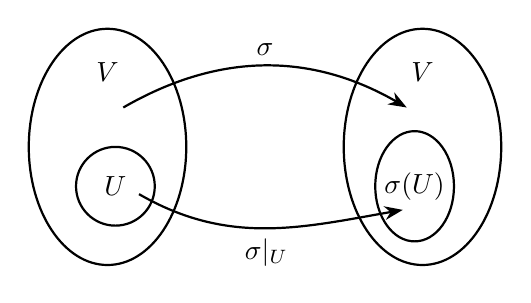
\begin{tikzpicture}[>=Stealth]
        \draw[thick] (-2,0) ellipse (1 and 1.5) node[above=20] {$V$}
        (2,0) ellipse (1 and 1.5) node[above=20] {$V$}
        (-1.9,-0.5) circle (0.5) node {$U$}
        (1.9,-0.5) ellipse (0.5 and 0.7) node {$\sigma(U)$}
        (-1.8,0.5) edge[out=30,in=150,->] node[above] {$\sigma$} (1.8,0.5)
        (-1.6,-0.6) edge[out=-30,in=190,->] node[below] {$\sigma\vert_U$} (1.75,-0.8);
    \end{tikzpicture}
\end{figure}

因此,如果$U$是$\sigma$的不变子空间,根据不变子空间的定义可知,$\sigma\vert_U$就是一个线性变换(是$\mathcal{L}(U)$中的元素),我们称之为\term{限制变换}\index{xianxingyingshe!xianxingbianhuan!xianzhi@限制变换 (restriction operator)}.

有了上面的概念,我们很容易可以将之前的推导转化为以下定理:
\begin{theorem}{}{不变子空间与分块对角矩阵}
    设有限维线性空间$V$上的线性变换$\sigma\in\mathcal{L}(V)$在某组基下的表示矩阵为分块对角矩阵$A=\diag(A_1,\ldots,A_m)$,当且仅当$V$可以分解为不变子空间$U_1,\ldots,U_m$的直和,即
    \[V=U_1\oplus\cdots\oplus U_m,\]
    其中每个$U_i$都是$\sigma$的不变子空间,且$\sigma\vert_{U_i}$在$U_i$对应的基下的表示矩阵为$A_i$.
\end{theorem}

根据定义我们可以验证或者求解一些很简单的不变子空间. 例如设$T\in \mathcal{L}(V)$,则$V$的两个平凡子空间$\{0\}$和$V$,以及映射的像与核$\ker T,\im T$都是$\sigma$不变子空间,验证非常简单,此处不赘述. 事实上当$p$为多项式时,$\ker p(\sigma)$和$\im p(\sigma)$也为$\sigma$的不变子空间. 我们这里也简要书写一下,供读者熟悉如何利用定义验证不变子空间:
\begin{example}{}{多项式不变子空间}
    若$\sigma\in\mathcal{L}(V)$且$p\in\mathbf{F}[x]$为多项式,则$\ker p(\sigma)$和$\im p(\sigma)$在$\sigma$下不变.
\end{example}

\begin{proof}
    我们只需验证$\ker p(\sigma)$和$\im p(\sigma)$中的元素经过$\sigma$映射后仍在这一空间中即可.
    \begin{enumerate}
        \item $\forall \alpha\in \ker p(\sigma),\enspace p(\sigma)\alpha=0$,因此
              \[(p(\sigma))(\sigma(\alpha))=\sigma(p(\sigma)\alpha)=\sigma(0)=0,\]
              即$\sigma(\alpha)\in \ker p(\sigma)$,因此$\ker p(\sigma)$在$\sigma$下不变;

        \item $\forall \alpha\in \im p(\sigma),\enspace \exists \beta\in V,\enspace \alpha=p(\sigma)\beta$,因此
              \[\sigma(\alpha)=\sigma(p(\sigma)\beta)=p(\sigma)(\sigma(\beta))\in \im p(\sigma),\]
              即$\im p(\sigma)$在$\sigma$下不变.
    \end{enumerate}
    事实上,对于$\ker p(\sigma)$,我们有
    \[ p(\sigma)(\alpha)=p(\sigma)\alpha=p(\sigma(\alpha))=p(0)=0,\]
    因此$\sigma(\alpha)\in \ker p(\sigma)$,即$\ker p(\sigma)$在$\sigma$下不变. 对于$\im p(\sigma)$,我们有
    \[\forall \alpha\in \im p(\sigma),\enspace \exists \beta\in V,\enspace \alpha=p(\sigma)\beta,\]
    因此
    \[\sigma(\alpha)=\sigma(p(\sigma)\beta)=p(\sigma)\sigma(\beta)\in \im p(\sigma),\]
    即$\im p(\sigma)$在$\sigma$下不变.
\end{proof}

有时我们可能会遇到更为复杂的情形,如下面的例子:
\begin{example}{}{不变子空间}
    设$\mathbf{F}$为一数域,线性变换$\sigma\in\mathcal{L}(\mathbf{F}^2)$定义为
    \[\sigma(a,b)=(a,b)\begin{pmatrix}
            1 & -1 \\ 2 & 2
        \end{pmatrix}\]
    证明:
    \begin{enumerate}
        \item 当$\mathbf{F}=\mathbf{R}$时,$\mathbf{R}^2$无$\sigma$的非零真不变子空间;

        \item 当$\mathbf{F}=\mathbf{C}$时,$\mathbf{C}^2$有$\sigma$的非零真不变子空间.
    \end{enumerate}
\end{example}

\begin{proof}
    事实上,由于$\sigma$定义在二维空间$\mathbf{F}^2$上,因此``非零真不变子空间''只能是一维子空间. 设该不变子空间$U=\spa(\alpha)(\alpha\neq 0)$,并进一步设$\alpha=(a,b)$. 我们知道,一维线性空间中所有元素都是成比例的(可以理解为一条直线,或者一维空间是由一个向量线性扩张而来,扩张过程中的线性组合一定保证后面生成的所有向量都互相成比例). 我们假设比例值为$\lambda$,即
    \[\sigma(a,b)=(a,b)\begin{pmatrix}
            1 & -1 \\ 2 & 2
        \end{pmatrix}=\lambda(a,b)=(\lambda a,\lambda b),\]
    将矩阵乘法展开,我们有
    \[(a+2b,-a+2b)=(\lambda a,\lambda b).\]
    由于$\alpha=(a,b)\neq 0$,因此$\lambda\neq 0$,基于此解方程得到$\lambda^2-3\lambda+4=0$. 这一方程在实数域范围内无解,复数域内有两个共轭的解,因此,我们有
    \begin{enumerate}
        \item 当$\mathbf{F}=\mathbf{R}$时,$\mathbf{R}^2$无$\sigma$的非零真不变子空间;

        \item 当$\mathbf{F}=\mathbf{C}$时,$\mathbf{C}^2$有$\sigma$的非零真不变子空间.
    \end{enumerate}
\end{proof}

除此之外,还有一些更为困难的问题我们将在讨论完标准形理论之后反过来进行讨论. 为了接下来对标准形讨论的方便,我们需要介绍一个特别的不变子空间:
\begin{definition}{}{循环子空间}
    设$T\in\mathcal{L}(V)$,$v\in V$是一个非零向量. 我们称子空间
    \[W=\spa(v,Tv,T^2v,\ldots,T^kv,\cdots)\]
    为\term{由$v$生成的$T\text{-循环子空间}$}. 在不引起歧义的情况下,我们也称$W$为\term{$T\text{-循环子空间}$}或\term{循环子空间}.
\end{definition}

一个需要注意的地方是,当$V$是有限维线性空间时,循环子空间也一定是有限维的(子空间的维数至少要小于等于原空间). 一个有趣的事实是,如果循环子空间的维数等于$m$,那么它的一组基就是$\{v,Tv,\ldots,T^{m-1}v\}$. 我们来书写这一定理并给出证明:
\begin{theorem}{}{循环子空间}
    设$V$是有限维线性空间,$T\in\mathcal{L}(V)$,$v\in V$是一个非零向量,$W$是由$v$生成的$T-\text{循环子空间}$,则
    \begin{enumerate}
        \item $W$是$T$包含$v$的最小不变子空间;
        \item 若$W$的维数为$m$,则$W$的一组基为$\{v,Tv,\ldots,T^{m-1}v\}$(我们称其为一组循环基).
    \end{enumerate}
\end{theorem}
\begin{proof}
    \begin{enumerate}
        \item 首先我们证明是不变子空间. 由于$V$是有限维线性空间,故$W$一定也是有限维线性空间,故任意的$w\in W$都可以被表示为$W$中有限个元素的线性组合,假设为
              \[w=k_1T^{m_1}v+k_2T^{m_2}v+\cdots+k_sT^{m_s}v,\]
              其中$m_1,m_2,\ldots,m_s\in\mathbf{N}$,$k_1,k_2,\ldots,k_s\in\mathbf{F}$. 我们有
              \[\begin{aligned}
                      Tw & =T(k_1T^{m_1}v+k_2T^{m_2}v+\cdots+k_sT^{m_s}v)     \\
                         & =k_1T^{m_1+1}v+k_2T^{m_2+1}v+\cdots+k_sT^{m_s+1}v,
                  \end{aligned}\]
              因此$Tw$仍然是$W$中向量的线性组合,即$Tw\in W$,故$W$是$T$的不变子空间.

              接下来我们证明是最小不变子空间. 设$U$是$T$的不变子空间,且$v\in U$,我们需要证明$W\subset U$. 由不变子空间的定义以及$v\in U$,我们知道$Tv\in U$,于是进一步利用不变子空间的定义有$T^2v\in U$,以此类推,$T^kv\in U,\enspace\forall k\in\mathbf{N}$,因此$W\subset U$,即$W$是$T$包含$v$的最小不变子空间.

        \item 由于$v$是非零向量,故设$j$是使得$v,Tv,\ldots,T^{j-1}v$线性无关的最大正整数,设$U=\spa(v,Tv,\ldots,T^{j-1}v)$,因此$v,Tv,\ldots,T^{j-1}v$是$U$的一组基. 并且根据我们的假设,$v,Tv,\ldots,T^{j-1}v,T^jv$线性相关,因此根据线性相关性质有
              \[T^jv=k_1v+k_2Tv+\cdots+k_{j-1}T^{j-1}v,\]
              即$T^jv\in U$,于是我们任取$u\in U$,有
              \[u=c_1v+c_2Tv+\cdots+c_{j-1}T^{j-1}v,\]
              因此
              \[Tu=c_1Tv+c_2T^2v+\cdots+c_{j-1}T^jv\in U,\]
              故$U$是$T$的包含$v$的不变子空间. 由定理第一条可知,$W\subset U$,但根据$U$的定义又有$U\subset W$,因此$W=U$,即$W$的一组基为$\{v,Tv,\ldots,T^{j-1}v\}$,故事实上$j$就是$W$的维数. 因此若$W$的维数为$m$,则$W$的一组基为$\{v,Tv,\ldots,T^{m-1}v\}$.
    \end{enumerate}
\end{proof}

最后我们再基于不变子空间讨论一个商线性变换的概念. 事实上,如果$U$是$\sigma$的不变子空间,那么$\sigma$还可以诱导出商空间$V/U$上的线性变换. 定义如下:
\begin{definition}{}{}
    设$\sigma\in \mathcal{L}(V)$,$U$是$\sigma$的不变子空间,定义映射$\sigma/U:V/U\to V/U$如下:
    \[(\sigma/U)(v+U)=\sigma(v)+U,\enspace\forall v\in V,\]
    则称$\sigma/U$是$\sigma$在$U$上的\term{商线性变换}\index{xianxingbianhuan@shang!商线性变换 (quotient operator)}.
\end{definition}

定义映射后,我们自然的想法就失确认这一定义是不是合理的. 首先这一定义的线性性容易验证,我们只需要用到商空间中定义的运算性质即可:
\begin{itemize}
    \item 齐次性:$(\sigma/U)(\lambda(v+U))=(\sigma/U)(\lambda v+U)=\sigma(\lambda v)+U=\lambda\sigma(v)+U=\lambda(\sigma/U)(v+U)$;

    \item 加性:$(\sigma/U)((v_1+U)+(v_2+U))=(\sigma/U)(v_1+v_2+U)=\sigma(v_1+v_2)+U=\sigma(v_1)+\sigma(v_2)+U=(\sigma/U)(v_1+U)+(\sigma/U)(v_2+U)$.
\end{itemize}

除了线性的要求外,还有一个很重要的合理性来源于之前在等价类和商空间中讨论的相容性(或者良定义)的概念,因为这里将线性变换定义在了等价类上. 事实上,对于一个映射,其相容性的关键在于原像集合中的同一个元素只能映射到像集中的唯一一个值(否则不符合映射的定义),具体而言,商线性变换的出发空间元素是等价类,因此如果出现$v+U=w+U$但$\sigma(v)+U\neq \sigma(w)+U$的情况,这一定义描述的就不是映射(因为映射要求一个自变量只能映到一个值上). 我们可以验证这一映射是满足相容性的:

\begin{proof}
    设$v+U=w+U$,即$v-w\in U$,由于$U$在$\sigma$下不变,则$\sigma(v-w)\in U$,即$\sigma(v)-\sigma(w)\in U$,因此$\sigma(v)+U=\sigma(w)+U$,即$\sigma/U$是满足相容性的.
\end{proof}

\section{特征值与特征向量}

在\autoref{thm:不变子空间与分块对角矩阵} 中我们得到了一个很关键的观察,就是不变子空间与分块对角矩阵的关联. 因此我们很自然地希望展开对不变子空间的研究,研究原空间是否能,以及怎么能分解为合理的不变子空间的直和,得到令人满意的简单的矩阵表示. 我们自然需要从最简单的不变子空间开始我们的研究,即一维的不变子空间.

事实上,在\autoref{ex:不变子空间} 中,我们已经尝试求解了一维不变子空间. 根据一维空间中向量都成比例的性质,设$U$是$\sigma\in\mathcal{L}(V)$的一维不变子空间,我们有
\[\exists\lambda\in\mathbf{F},\enspace\sigma(\alpha)=\lambda\alpha,\enspace\forall \alpha\in U,\]
即任意向量作用线性变换后的结果与原向量成比例. 这一性质将引入接下来的特征值与特征向量的概念,事实上它们对于获得简单矩阵的目标而言非常重要,因此是我们讨论的很好的开始.

在接下来的讨论中,我们很多定义和结论都会有相应的矩阵和映射版本. 回顾在\autoref{thm:线性映射对向量坐标的影响} 中的讨论,我们提到了矩阵$A$和线性映射$\sigma(\alpha)=A\alpha$的统一性,并且在相似的引入中我们也提到了我们的目标在线性变换和矩阵两个角度下的陈述及其关联,因此我们未来将不特别区分矩阵和线性变换,这一点在本节过后将有更深刻的体会.

\subsection{特征值与特征向量的定义与求解}

首先介绍线性变换和矩阵的特征值与特征向量的概念:
\begin{definition}{}{}
    设$\sigma$是线性空间$V(\mathbf{F})$上的一个线性变换,如果存在数$\lambda\in\mathbf{F}$和非零向量$\xi\in V$使得$\sigma(\xi)=\lambda\xi$,则称数$\lambda$为$\sigma$的一个\term{特征值}\index{tezhengzhi@特征值 (eigenvalue)},并称非零向量$\xi$为$\sigma$属于其特征值$\lambda$的\term{特征向量}\index{tezhengxiangliang@特征向量 (eigenvector)}.
\end{definition}
必须注意特征向量为非零向量,否则零向量$\xi=\vec{0}$对任意$\lambda$都满足上面定义,从而失去``特征''的含义. 但是特征值可以为0,此时$\sigma(\xi)=\vec{0}$,即全体特征向量的集合就是线性变换的核空间.

对于某一个$\lambda\in\mathbf{F}$,我们将所有满足$\sigma(\xi)=\lambda\xi$的向量构成的集合记为$E(\lambda,\sigma)=\{\xi \mid \sigma(\xi)=\lambda\xi,\enspace\xi\in V\}$(在去除线性变换不引起歧义的情况下可简写为$V_\lambda$),称为$\sigma$关于其特征值$\lambda$的\term{特征子空间}\index{tezhengzikongjian@特征子空间 (eigenspace)}. 显然,这一集合是由零向量和全体$\lambda$对应的特征向量构成的. 我们可以验证$V_\lambda$的确是$V$的``子空间'':
\begin{example}{}{}
    证明:$V_\lambda$是$V$的子空间,并且是线性变换$\sigma$的不变子空间.
\end{example}

\begin{proof}
    回顾证明子空间的两个要求:非空和运算封闭性. 首先$V_\lambda$非空,因为$\vec{0}\in V_\lambda$,即$\sigma(\vec{0})=\lambda\vec{0}$,因此$\vec{0}\in V_\lambda$,故$V_\lambda$非空.

    其次,对于任意$\xi_1,\xi_2\in V_\lambda$,$k_1,k_2\in\mathbf{F}$,我们有
    \[\sigma(k_1\xi_1+k_2\xi_2)=k_1\sigma(\xi_1)+k_2\sigma(\xi_2)=k_1\lambda\xi_1+k_2\lambda\xi_2=\lambda(k_1\xi_1+k_2\xi_2),\]
    因此$k_1\xi_1+k_2\xi_2\in V_\lambda$,故满足线性运算封闭. 综上,$V_\lambda$是$V$的子空间.

    不变子空间也是显然的. 对于任意$\xi\in V_\lambda$,因为$V_\lambda$是由零向量和全体$\lambda$对应的特征向量构成的,因此必有$\sigma(\xi)=\lambda\xi\in V_\lambda$,因此$V_\lambda$是$\sigma$的不变子空间.
\end{proof}

事实上,我们通过之后的例子会知道,$V_\lambda$的维数不一定是1,而至少是1. 那么我们之前引入特征值特征向量时所说的``一维不变子空间''是什么呢?事实上,我们可以取$V_\lambda$的任一组基$\alpha_1,\ldots,\alpha_n$,则其中任一向量进行扩张得到的子空间$U_i=\spa(\alpha_i),\enspace i=1,\ldots,n$就是一维不变子空间,因为$\forall u_i\in U_i,\enspace \sigma(u_i)=\lambda u_i\in U_i$,即$U_i$在$\sigma$下不变. 我们还需要注意,一维不变子空间的选取是不唯一的,因为$V_\lambda$的基的选取是不唯一的,因此$U_i$的选取也是不唯一的,实际上对于任意的$\alpha\in\V_{\lambda}$,$\spa(\alpha)$都是一维不变子空间.

上面是线性变换的特征值与特征向量的定义. 然而我们有一个无法绕开的问题,就是基于线性变换计算特征值与特征向量似乎并不是一个程序化的过程. 因此我们需要求助于矩阵——这是一个适合于计算的良好工具. 对应的,我们给出矩阵的特征值与特征向量的定义:
\begin{definition}{}{}
    设矩阵$A\in \mathbf{M}_n(\mathbf{F})$,如果存在数$\lambda\in\mathbf{F}$和非零向量$X\in\mathbf{F}^n$使得$AX=\lambda X$,则称数$\lambda$为$A$的一个特征值,称非零向量$X$为$A$属于其特征值$\lambda$的特征向量.
\end{definition}

下面我们说明线性映射的特征值与特征向量和矩阵的特征值与特征向量之间的关系. 实际上,假设$A$是$\sigma$在基$\alpha_1,\ldots,\alpha_n$下的表示矩阵,且$\xi=(\alpha_1,\ldots,\alpha_n)X$,即$X$是$\xi$在基$\alpha_1,\ldots,\alpha_n$下的坐标,则我们有
\begin{align*}
    \sigma(\xi)=\lambda\xi & \iff \sigma((\alpha_1,\ldots,\alpha_n)X)=\lambda(\alpha_1,\ldots,\alpha_n)X        \\
                           & \iff (\sigma(\alpha_1,\ldots,\alpha_n))X=(\lambda\alpha_1,\ldots,\lambda\alpha_n)X \\
                           & \iff (\alpha_1,\ldots,\alpha_n)AX=(\alpha_1,\ldots,\alpha_n)(\lambda X)            \\
                           & \iff AX=\lambda X
\end{align*}
其中第一行与第二行间的等价关系用到了矩阵乘法一节中证明的性质$\sigma((\alpha_1,\ldots,\alpha_n)X)=(\sigma(\alpha_1,\ldots,\alpha_n))X$. 由上述讨论可知$\lambda$同时是线性变换和矩阵的特征值,与基的选取无关. 但矩阵的特征向量$X$是线性映射特征向量在基下的坐标,这与基的选取有关. 由于基$\alpha_1,\ldots,\alpha_n$可以是任取的,于是求解线性变换的特征值的问题完全转化为了求线性变换任意一个矩阵表示的特征值,而特征向量也仅仅是向量与坐标的关系. 于是接下来我们讨论如何具体求解特征值与特征向量. 我们首先需要证明一个定理做一个简单的观察:
\begin{theorem}{}{}
    设$\sigma$是$V(\mathbf{F})$上的线性变换,$I$为恒等映射,则下述条件等价:
    \begin{enumerate}[label=(\arabic*)]
        \item \label{item:18:特征值定义:1}
              $\lambda\in\mathbf{F}$是$\sigma$的特征值;

        \item \label{item:18:特征值定义:2}
              $\sigma-\lambda I$不是单射;

        \item \label{item:18:特征值定义:3}
              $\sigma-\lambda I$不是满射;

        \item \label{item:18:特征值定义:4}
              $\sigma-\lambda I$不可逆.
    \end{enumerate}
\end{theorem}

\begin{proof}
    \begin{itemize}
        \item[\ref*{item:18:特征值定义:1}$\implies$\ref*{item:18:特征值定义:2}] $\lambda\in\mathbf{F}$是$\sigma$的特征值,说明$\exists v\in V$且$v\neq 0$使得$\sigma(v)=\lambda v$. 因此$(\sigma-\lambda I)(v)=0$,即$\sigma-\lambda I$核空间不只有零元,根据单射等价条件\autoref{thm:单射与核空间},不单成立;

        \item[\ref*{item:18:特征值定义:2}$\implies$\ref*{item:18:特征值定义:3}] 根据\autoref{thm:双射等价条件} 可知,$\sigma-\lambda I$不满当且仅当$\sigma-\lambda I$不单;

        \item[\ref*{item:18:特征值定义:3}$\implies$\ref*{item:18:特征值定义:4}] 根据\autoref*{thm:双射等价条件} 显然;

        \item[\ref*{item:18:特征值定义:4}$\implies$\ref*{item:18:特征值定义:1}] $\sigma-\lambda I$不可逆,根据\autoref*{thm:双射等价条件} 可知其不为单射,又根据单射等价条件\autoref*{thm:单射与核空间} 可知$(\sigma-\lambda I)(v)=0$有非零解,即$\sigma(v)=\lambda v$,其中$v\neq 0$,这与特征值定义一致.
    \end{itemize}
\end{proof}

由上述定理,$\lambda\in\mathbf{F}$是$\sigma$的特征值等价于$\sigma-\lambda I$不可逆,因此其在$V$的任意一组基$\alpha_1,\ldots,\alpha_n$下的矩阵$A-\lambda E$也不可逆(其中$A$为$\sigma$在这组基下的矩阵,$E$为单位矩阵),这又等价于$|A-\lambda E|=0$.

因此$\lambda\in\mathbf{F}$是$\sigma$的特征值等价于$|\lambda E-A|=0$,故我们可以通过$|\lambda E-A|=0$求解特征值,其中$A$为$\sigma$在某组基下的矩阵,$E$为单位矩阵. 对于特征向量的求解,求出$(\lambda E-A)X=0$的非零解就是特征向量在基$\alpha_1,\ldots,\alpha_n$下的坐标,如果是矩阵的特征向量,那么$X$就是解.

上述求解特征向量的方法需要我们求解$f(\lambda)=|\lambda E-A|$的根,事实上$f(\lambda)=|\lambda E-A|$是在之后的讨论中有核心地位的概念,我们称其为矩阵$A$的\term{特征多项式}\index{tezhengduoxiangshi@特征多项式 (characteristic polynomial)},其$k$重根称为$k$重特征值(称$k$为代数重数),该特征值对应的特征子空间维数称为该特征值的几何重数.

\begin{example}{}{}
    设$A=\begin{pmatrix}
            1 & -1 & 0 \\ 2 & 0 & 1 \\ 1 & a & 0
        \end{pmatrix}$,且存在非零向量$\alpha$使得$A\alpha=2\alpha$,求$a$.
\end{example}

\begin{solution}
    由题意知2是矩阵$A$的特征值,因此我们有
    \[|2E-A|=\begin{vmatrix}
            1 & 1 & 0 \\ -2 & 2 & -1 \\ -1 & -a & 2
        \end{vmatrix}=9-a=0,\]
    因此$a=9$.
\end{solution}

接下来,我们将特征多项式定义中的行列式展开得到以下定理:
\begin{theorem}{}{特征多项式展开}
    对于$n$级矩阵$A=(a_{ij})$,记
    \[f(\lambda)=|\lambda E-A|=a_0\lambda^n+a_1\lambda^{n-1}+\cdots+a_{n-1}\lambda+a_n\]
    则$a_0=1$,$a_1=-\tr(A)$,$a_n=(-1)^n|A|$,且$a_k$等于所有$k$级主子式之和乘以$(-1)^k$.
\end{theorem}

\begin{proof}
    设$A=(a_{ij})$的列向量为$\alpha_1,\ldots,\alpha_n$,则
    \[f(\lambda)=|\lambda E-A|=\begin{vmatrix}
            \lambda e_1-\alpha_1 & \lambda e_2-\alpha_2 & \cdots & \lambda e_n-\alpha_n
        \end{vmatrix}.\]
    其中$e_1,\ldots,e_n$为$\mathbf{F}^n$的标准基,因此根据行列式的\autoref{def:公理化定义} 的加性,$f(\lambda)$可以拆成$2^n$个行列式的和,它们是
    \begin{equation}\label{eq:18:特征多项式展开}
        (-\alpha_1,\ldots,-\alpha_{j_1-1},\lambda e_{j_1},-\alpha_{j_1+1},\ldots,-\alpha_{j_2-1},\lambda e_{j_2},-\alpha_{j_2+1},\ldots,-\lambda e_{j_{n-k}},\ldots,-\alpha_n),
    \end{equation}
    其中$1\leqslant j_1<j_2<\cdots<j_{n-k}\leqslant n,\enspace k=0,2,\ldots,n$.

    上式初看会显得非常复杂,但实际上利用行列式定义的加性去拆分就是每列有两种拆出来的选择,一种是选择$\lambda e_{j_i}$,另一种是选择$-\alpha_{j_i}$,这就是$2^n$种拆分方式的来由. 其中取出$k$列$-\alpha_{j_i}$,剩余$n-k$列选择$\lambda e_{j_i}$的就可以表示为上式的形式.

    利用\autoref{thm:Laplace定理} 对\autoref{eq:18:特征多项式展开} 第$j_1,\ldots,j_{n-k}$列展开,我们发现这$n-k$列元素组成的$n-k$阶子式只有一个不为0:
    \[\begin{vmatrix}
            \lambda & 0       & \cdots & 0       \\
            0       & \lambda & \cdots & 0       \\
            \vdots  & \vdots  & \ddots & \vdots  \\
            0       & 0       & \cdots & \lambda
        \end{vmatrix}=\lambda^{n-k},\]
    这个不等于0的$n-k$阶子式对应的代数余子式为
    \begin{align*}
         & (-1)^{(j_1+\cdots+j_{n-k})+(j_1+\cdots+j_{n-k})}(-A)
        \begin{pmatrix}
            j_1' & j_2' & \cdots & j_k' \\
            j_1' & j_2' & \cdots & j_k'
        \end{pmatrix}                             \\
         & = (-1)^kA\begin{pmatrix}
                        j_1' & j_2' & \cdots & j_k' \\
                        j_1' & j_2' & \cdots & j_k'
                    \end{pmatrix}
    \end{align*}
    其中$j_1',\ldots,j_k'$为$1,\ldots,n$中除去$j_1,\ldots,j_{n-k}$的$k$个数按递增顺序排列的结果,这一点通过余子式的定义是显然的. 因此\autoref{eq:18:特征多项式展开} 的值为
    \[(-1)^kA\begin{pmatrix}
            j_1' & j_2' & \cdots & j_k' \\
            j_1' & j_2' & \cdots & j_k'
        \end{pmatrix}\lambda^{n-k}.\]
    这实际上只是取$n-k$列$\lambda e_{j_i}$的一种情况,事实上对于所有可能的$j_1,\ldots,j_{n-k}$的取法,我们都可以得到类似的结果,因此$|\lambda E-A|$中$\lambda^{n-k}$的系数为
    \[(-1)^k\sum\limits_{1\leqslant j_1'<\cdots<j_k'\leqslant n}A\begin{pmatrix}
            j_1' & j_2' & \cdots & j_k' \\
            j_1' & j_2' & \cdots & j_k'
        \end{pmatrix}.\]
    即$a_k$等于所有$k$级主子式之和乘以$(-1)^k$,且代入$k=0,1,n$有$a_0=1$,$a_1=-\tr(A)$,$a_n=(-1)^n|A|$.
\end{proof}

这一定理的证明事实上无需掌握,这里给出证明是为了补全教材中的空缺. 这里我们主要掌握两个特例,即由韦达定理,我们有
\begin{enumerate}
    \item $\displaystyle\sum_{i=1}^{n}\lambda_i=\sum_{i=1}^{n}a_{ii}$;

    \item $\displaystyle\prod_{i=1}^{n}\lambda_i=|A|$.
\end{enumerate}
即特征值按重数求和为矩阵的迹(即矩阵对角线元素之和),特征值按重数求积为矩阵行列式. 这一结论在解决某些问题时有一定作用.

事实上,我们这里给出的特征多项式只是矩阵的特征多项式的定义,关于线性变换特征多项式的定义以及进一步讨论将在后续章节进行,我们也会说明两种特征多项式的定义是统一的.

\subsection{相似与特征值、特征向量的关联}
可能细心的读者已经发现,我们前面的讨论中的某个位置留下了一个bug. 我们在讨论线性变换与矩阵的特征值的关联时,提到我们可以取线性变换任意一组基下的表示矩阵来计算特征值,这些特征值就是线性变换的特征值. 事实上这暗示了一个很重要的性质:线性变换任意一组基下的矩阵都有相同的特征值,或者说,相似的矩阵就有相同的特征值,否则上面的讨论一定是有问题的. 我们在此叙述这一性质并给出证明:
\begin{theorem}{}{}
    相似矩阵有相同的特征多项式(逆命题不成立),即$A\sim B$有$|\lambda E-A|=|\lambda E-B|$,从而有相同的迹,行列式,特征值,但特征向量不一定相同.
\end{theorem}
\begin{proof}
    设$B=P^{-1}AP$,则$|\lambda E-B|=|\lambda E-P^{-1}AP|=|P^{-1}(\lambda E-A)P|=|P^{-1}||\lambda E-A||P|=|\lambda E-A|$. 因此$A\sim B$有$|\lambda E-A|=|\lambda E-B|$.

    我们知道特征多项式相同则特征值相同,迹等于所有特征值之和,行列式等于所有特征值之积,因此相似矩阵有相同的迹,行列式,特征值.

    相似矩阵来源于同一线性变换在不同基下的表示,因此它们的特征向量是线性变换的特征向量在不同基下的坐标,因此不一定相同.
\end{proof}

在得到这一结论后,我们同样可以定义线性变换的特征多项式:我们就可以定义其为任意矩阵表示的特征多项式.
\begin{definition}{}{}
    设$\sigma$是$V(\mathbf{F})$上的线性变换,$A$是$\sigma$在任意一组基下的矩阵,则$\sigma$的\term{特征多项式}\index{tezhengduoxiangshi@特征多项式 (characteristic polynomial)}定义为$|\lambda E-A|$.
\end{definition}

下面我们讨论一些重要的例子. 首先要引入的例子也是重要的结论,实际上在行列式一讲中已给出类似结论,但我们现在从特征值角度考虑这一结论:
\begin{example}{}{}
    回答以下两个问题:
    \begin{enumerate}
        \item \label{item:18:特征值相同:1}
              设$A,B$均为$n$阶矩阵,证明:$\lambda\neq 0$是$AB$的特征值,则$\lambda$也是$BA$的特征值;

        \item \label{item:18:特征值相同:2}
              设$A\in \mathbf{M}_{m\times n}(\mathbf{C}),\enspace B\in \mathbf{M}_{n\times m}(\mathbf{C})$,证明:
              \[ \begin{pmatrix}
                      AB & O \\ B & O
                  \end{pmatrix}\sim\begin{pmatrix}
                      O & O \\ B & BA
                  \end{pmatrix} \]
              并由此推出$AB$和$BA$非零特征值相同,且$m=n$时有$|\lambda E-AB|=|\lambda E-BA|$.
    \end{enumerate}
\end{example}

\begin{proof}
    \begin{enumerate}
        \item 设$X$是$AB$属于$\lambda$的特征向量,则$ABX=\lambda X$,因此$B(ABX)=B(\lambda X)$,即$(BA)(BX)=\lambda(BX)$,因此$BX$是$BA$属于$\lambda$的特征向量,故$\lambda$也是$BA$的特征值.

              实际上这里还有一点需要说明,就是$BX\neq 0$,否则它将不能作为特征向量. 事实上证明是简单的,假设$BX=0$,则$ABX=0$,由于$\lambda\neq 0$,因此必然有$X=0$,但这与$X$是$AB$属于$\lambda$的特征向量矛盾,因此$BX\neq 0$.

        \item 根据分块矩阵初等变换的性质,我们可以通过不断尝试选取到$P=\begin{pmatrix}
                      E_m & A \\ O & E_n
                  \end{pmatrix}$,其逆矩阵为$P^{-1}=\begin{pmatrix}
                      E_m & -A \\ O & E_n
                  \end{pmatrix}$,我们发现恰有
              \[\begin{pmatrix}
                      E_m & -A \\ O & E_n
                  \end{pmatrix}\begin{pmatrix}
                      AB & O \\ B & O
                  \end{pmatrix}\begin{pmatrix}
                      E_m & A \\ O & E_n
                  \end{pmatrix}=\begin{pmatrix}
                      O & O \\ B & BA
                  \end{pmatrix}.\]
              因此$\begin{pmatrix}
                      AB & O \\ B & O
                  \end{pmatrix}$与$\begin{pmatrix}
                      O & O \\ B & BA
                  \end{pmatrix}$相似,因此它们的特征多项式相同,即
              \[\begin{vmatrix}
                      \lambda E_m-AB & O \\ -B & \lambda E_n
                  \end{vmatrix}=\begin{vmatrix}
                      \lambda E_m & O \\ -B & \lambda E_n-BA
                  \end{vmatrix}.\]
              根据行列式的计算性质$\begin{vmatrix}
                      A & O \\ C & B
                  \end{vmatrix}=|A||B|$,我们有
              \[|\lambda E_m-AB||\lambda E_n|=|\lambda E_m||\lambda E_n-BA|,\]
              即$\lambda^n|\lambda E_m-AB|=\lambda^m|\lambda E_n-BA|$,因此$AB$和$BA$非零特征值相同,且$m=n$时有$|\lambda E-AB|=|\lambda E-BA|$.
    \end{enumerate}
\end{proof}

不难发现上述例子中 \ref*{item:18:特征值相同:2} 是 \ref*{item:18:特征值相同:1} 的推广,因为由\ref*{item:18:特征值相同:2} 我们得到了$|\lambda E-AB|=|\lambda E-BA|(\lambda\neq 0)$.

下面这个例子非常重要,在解决一些题目时使用这一结论会更便捷:
\begin{example}{}{}
    (\autoref{thm:基的选择对向量坐标的影响} 推广)设$P^{-1}AP=B$,证明:$A,B$分别属于同一特征值$\lambda$的特征向量$X$和$Y$满足$Y=P^{-1}X$.
\end{example}

\begin{proof}
    由$AX=\lambda_0 X$以及$A=PBP^{-1}$,我们有$PBP^{-1}X=\lambda_0 X$,即$BP^{-1}X=\lambda_0 P^{-1}X$,因此$P^{-1}X$是$B$属于$\lambda_0$的特征向量,即$P^{-1}X$是$B$的特征向量,即$Y=P^{-1}X$.
\end{proof}

实际上本题是本讲义\autoref{thm:基的选择对向量坐标的影响} 的推论,原因在于$P^{-1}AP=B$说明$A$和$B$是同一个线性变换(设为$\sigma$)在不同基下的矩阵,因此$X$和$Y$只是$\sigma$关于$\lambda_0$在两组基下的坐标,因此二坐标之间相差一个过渡矩阵.

最后我们谈一个拓展题型,我们考虑矩阵方程$AX-XB=O$,若$A,B$都是$n$阶方阵且$X$可逆,则方程可以改写为$X^{-1}AX=B$,即$A$与$B$相似. 事实上,这一矩阵方程的解空间的维数实际上刻画了$A$与$B$的相似程度. 我们有如下结论:
\begin{theorem}{}{}
    设$A,B$分别为数域$\mathbf{F}$上$n$阶、$m$阶方阵,$A,B$有$r$个两两不等的公共特征值,则矩阵方程$AX-XB=O$有秩为$r$的矩阵解. 反之,若数域为复数域,矩阵方程$AX-XB=O$有秩为$r$的矩阵解,则$A,B$至少有$r$个公共的特征值(计重数).
\end{theorem}

\begin{proof}
    \begin{enumerate}
        \item 设$\lambda_1,\ldots,\lambda_r$是$A$和$B$的$r$个公共特征值,$\alpha_1,\ldots,\alpha_r$为$A$相应的特征向量. 由于$\lambda_1,\ldots,\lambda_r$也是$B^\mathrm{T}$的特征值,设$\beta_1,\ldots,\beta_r$是$B^\mathrm{T}$相应的特征向量. 则$B^\mathrm{T}\beta_i=\lambda_i\beta_i$,从而$\beta_i^{\mathrm{T}}B=\lambda\beta_i^{\mathrm{T}}$. 下面我们证明$X=(\alpha_1,\ldots,\alpha_r)\cdot(\beta_1,\ldots,\beta_r)^\mathrm{T}$是$AX-XB=0$的解.

        事实上,$AX=A(\alpha_1,\ldots,\alpha_r)\cdot(\beta_1,\ldots,\beta_r)^\mathrm{T}=(\lambda_1\alpha_1,\ldots,\lambda_r\alpha_r)\cdot(\beta_1,\ldots,\beta_r)^\mathrm{T}=\lambda_1\alpha_1\beta_1+\cdots+\lambda_r\alpha_r\beta_r$,$XB=(\alpha_1,\ldots,\alpha_r)\cdot(\beta_1,\ldots,\beta_r)^\mathrm{T}B=(\alpha_1,\ldots,\alpha_r)\cdot(\lambda_1\beta_1,\ldots,\lambda_r\beta_r)=(\lambda_1\alpha_1\beta_1+\cdots+\lambda_r\alpha_r\beta_1)$. 故$AX-XB=0$.

        接下来证明$r(X)=r$.
        注意到$r(\alpha_1,\ldots,\alpha_r)=r((\beta_1,\ldots,\beta_r)^\mathrm{T})=r$,故$r(X)\leqslant r(\alpha_1,\ldots,\alpha_r)=r,r(X)\geqslant r(\alpha_1,\ldots,\alpha_r)+r((\beta_1,\ldots,\beta_r)^\mathrm{T})-r$,从而$r(X)=r$.
        \item 设$X=P\begin{pmatrix}
            E_r & 0 \\
            0 & 0
        \end{pmatrix}Q$,则$AX-XB=0$,从而$P^{-1}AP\begin{pmatrix}
            E_r & 0 \\
            0 & 0
        \end{pmatrix} =
        \begin{pmatrix}
            E_r & 0 \\
            0 & 0
        \end{pmatrix}QBQ^{-1}$.

        设$C=P^{-1}AP=\begin{pmatrix}
            C_1 & C_2 \\
            C_3 & C_4
        \end{pmatrix}$,
        $D=QBQ^{-1}=\begin{pmatrix}
            D_1 & D_2 \\
            D_3 & D_4
        \end{pmatrix}$. 则
        $\begin{pmatrix}
            C_1 & C_2 \\
            C_3 & C_4
        \end{pmatrix}\begin{pmatrix}
            E_r & 0 \\
            0 & 0
        \end{pmatrix} = \begin{pmatrix}
            E_r & 0 \\
            0 & 0
        \end{pmatrix}\begin{pmatrix}
            D_1 & D_2 \\
            D_3 & D_4
        \end{pmatrix}$,从而知$C_1=D_1$,$C_2=D_3=0$.
        由于$|\lambda E-C|=|\lambda E_r-C_1||\lambda E_{n-r}-C_4|$,$|\lambda E-D|=|\lambda E_r-D_1||\lambda E_{m-r}-D_4|$,而$|\lambda E_r-C_1|$是一个关于$\lambda$的$r$次多项式,在复数域上有$r$个根(计重数),它们是$C$的特征值,同时也为$D$的特征值. 从而$C$和$D$至少有$r$个公共的特征值. 而相似变换不改变矩阵的特征值,这表明$A,B$至少有$r$个公共的特征值.
    \end{enumerate}
\end{proof}

由此可以看出,复数域上$n$阶、$m$阶方阵$A,B$的矩阵方程$AX=XB$只有零解的充要条件是$A,B$没有公共特征值. 我们通过一个例子应用这一定理:
\begin{example}{}{}
    设$m$阶矩阵$A$与$n$阶矩阵$B$无公共复特征值,$C$为$m\times n$矩阵,则矩阵方程$AX-XB=C$存在唯一解.
\end{example}

\begin{proof}
    设$V$是所有$m\times n$矩阵构成的线性空间,定义$V$上的线性变换$\sigma(X)=AX-XB,\enspace X\in V$. 由于$A$和$B$无公共复特征值,所以$\sigma(X)=AX-XB=O$只有零解,即$\sigma$为$V$上单射,由\autoref{thm:双射等价条件} 可知$\sigma$是满射且是同构映射. 于是,对任意的$C\in V$,都存在唯一的$X_0\in V$使得$\sigma(X_0)=C$,即矩阵方程$AX-XB=C$存在唯一解$X_0$.
\end{proof}

\subsection{特征值的基本性质}

关于特征值,我们有如下基本性质:
\begin{enumerate}
    \item 设$\lambda$是线性空间$V(\mathbf{F})$上的线性变换$\sigma$的特征值,$\xi$是$\sigma$属于$\lambda$的特征向量,则
          \begin{enumerate}
              \item $k\lambda$是$k\sigma$的特征值,$\lambda^m$是$\sigma^m$的特征值,且$\xi$仍是相应特征向量;

              \item 若$f(x)=a_nx^n+a_{n-1}x^{n-1}+\cdots+a_1x+a_0$是$\mathbf{F}$上的多项式,则$f(\sigma)(\xi)=f(\lambda)\xi$;
          \end{enumerate}

    \item 设$\lambda$是$n$阶矩阵$A$的特征值,$A$可逆,则$\lambda^{-1}$是$A^{-1}$的特征值,$|A|\lambda^{-1}$是$A$的伴随矩阵$A^*$的特征值,且特征向量不变.

    \item 设$A$为$n$阶矩阵,则$A$与$A^\mathrm{T}$有相同的特征值(含重数).
\end{enumerate}

\begin{proof}
    \begin{enumerate}
        \item \begin{enumerate}
                  \item 由于$\sigma(\xi)=\lambda\xi$,则$(k\sigma)(\xi)=k\lambda\xi$,即$k\lambda$是$k\sigma$的特征值,$\xi$仍是相应特征向量.

                        而$\sigma^m(\xi)=\sigma^{m-1}(\sigma(\xi))=\sigma^{m-1}(\lambda\xi)=\lambda\sigma^{m-1}(\xi)=\cdots=\lambda^m\xi$,即$\lambda^m$是$\sigma^m$的特征值,$\xi$仍是相应特征向量.

                  \item 利用前述$\sigma^m$的相关性质,我们有
                        \begin{align*}
                            f(\sigma)(\xi) & = (a_n\sigma^n+a_{n-1}\sigma^{n-1}+\cdots+a_1\sigma+a_0I)(\xi)              \\
                                           & = a_n\sigma^n(\xi)+a_{n-1}\sigma^{n-1}(\xi)+\cdots+a_1\sigma(\xi)+a_0I(\xi) \\
                                           & = a_n\lambda^n\xi+a_{n-1}\lambda^{n-1}\xi+\cdots+a_1\lambda\xi+a_0\xi       \\
                                           & = f(\lambda)\xi.
                        \end{align*}
              \end{enumerate}

        \item 设$\xi$是$A$的特征值,即$A\xi=\lambda\xi$,则$\xi=A^{-1}A\xi=A^{-1}\lambda\xi$,即$A^{-1}\xi=\lambda^{-1}\xi$,因此$\lambda^{-1}$是$A^{-1}$的特征值,$\xi$仍是相应特征向量.

              又由于$A$可逆时$A^*=|A|A^{-1}$,根据前面关于$k\sigma$和$A^{-1}$特征值的讨论可知,$|A|\lambda^{-1}$是$A$的伴随矩阵$A^*$的特征值,$\xi$仍是相应特征向量.

        \item 我们用特征多项式证明. 实际上,$A^\mathrm{T}$的特征多项式为$|\lambda E-A^\mathrm{T}|=|(\lambda E-A)^\mathrm{T}|=|\lambda E-A|$(回忆转置不改变行列式),实际上与$A$的特征多项式完全一致,因此$A^\mathrm{T}$与$A$有相同的特征值(含重数).
    \end{enumerate}
\end{proof}

事实上,根据我们之前对线性变换特征值和矩阵特征值的讨论,我们知道上面的结论中``矩阵''和``线性变换''都可以互相替换(除了伴随矩阵没有定义相应的映射).

下面这一例子也是一些经典的结论,应当熟悉.
\begin{example}{}{特征值的性质}
    对下列矩阵$A$的特征值,能做出怎样的断言?
    \begin{enumerate}
        \item $A$可逆/$A$不可逆/$E+A$可逆/$4E+A$不可逆;

        \item $|E-A^2|=0$;

        \item $A^2=E$(对合)/$A^2=A$(幂等)/$A^k=0$(幂零);

        \item $A=\lambda_0E+B$($\lambda_0$为常数,且已知$B$的$n$个特征值为$\lambda_1,\lambda_2,\ldots,\lambda_n$);

        \item $A$为对角块矩阵,即$A=\diag(A_1,A_2,\ldots,A_m)$.
    \end{enumerate}
\end{example}

\begin{solution}
    \begin{enumerate}
        \item $A$可逆时有$|A|=\lambda_1\cdots\lambda_n\neq 0$,因此$A$的特征值都不为0. 同理,$A$不可逆同理表明存在特征值等于0,$E+A$可逆表明$-1$不是$A$的特征值,$4E+A$不可逆表明$-4$是$A$的特征值.

        \item $|E-A^2|=|E-A||E+A|=0$,因此$\pm 1$都是$A$的特征值.

        \item 我们首先考虑对合矩阵,接下来的同理可以得到类似结论. 由于$A^2=E$,设$AX=\lambda X$,则$A^2X=\lambda^2X=X$,因此$\lambda^2=1$,即$\lambda=\pm 1$,因此$1$或$-1$是$A$的特征值.

              但这里我们需要强调的是,不同于前两问,前两问中我们都是说某些值是$A$的特征值,但无法保证$A$的特征值只能是某些值,但在本题这样给出矩阵方程的情况下,我们可以得到$A$的特征值只能是$\pm 1$,没有其他值. 我们用反证法,假设存在$\lambda_0\neq\pm 1$是$A$的特征值,即$AX=\lambda_0X$,则$A^2X=\lambda_0^2X\neq X$(因为$X$不是零向量),导出矛盾. 当然有同学可能会思考,$A$的特征值一定兼有$\pm 1$吗,事实上并非如此,例如$E$满足$E^2=E$,但其特征值只有1,$-E$满足$(-E)^2=E$,但其特征值只有$-1$. 并且利用下一讲对角化的结论可以知道(我们放在下一讲习题中供读者练习),满足$A^2=E$且特征值只有1的矩阵只能是$E$,特征值只有$-1$的矩阵只能是$-E$.

              注:本题解决过程中告诉我们一个解题技巧,如果看到$A$的多项式$f(A)=O$这种形式的表达式,事实上$A$的特征值只能是$f(\lambda)=0$的根,如上题中$f(A)=A^2-E$,则$f(\lambda)=\lambda^2-1$,因此$A$的特征值只能是$\pm 1$.

              同理,我们可以知道幂等矩阵的特征值只能是0和1,幂零矩阵的特征值只能是0(这是一个重要的幂零矩阵等价条件,未来我们会再次遇到).

        \item 设$BX=\lambda_iX_i(X_i\neq 0,\enspace i=1,\ldots,n)$,则$AX_i=\lambda_0X_i+BX_i=\lambda_0X_i+\lambda_iX_i=(\lambda_0+\lambda_i)X_i$,因此$\lambda_0+\lambda_i\enspace(i=1,\ldots,n)$都是$A$的特征值.

        \item \begin{align*}
                  |\lambda E-A| & =\begin{vmatrix}
                                       \lambda E_1-A_1 & 0               & \cdots & 0               \\
                                       0               & \lambda E_2-A_2 & \cdots & 0               \\
                                       \vdots          & \vdots          & \ddots & \vdots          \\
                                       0               & 0               & \cdots & \lambda E_m-A_m
                                   \end{vmatrix}
                                & =\prod_{i=1}^{m}|\lambda E_i-A_i|=0
              \end{align*}
              因此,$A_i,\enspace i=1,\ldots,m$的特征值都是$A$的特征值.
    \end{enumerate}
\end{solution}

基于上面给出的性质和例子,我们可以进一步运用特征值的性质来求解一些问题,下面是一些例子:
\begin{example}{}{}
    回答以下问题:
    \begin{enumerate}
        \item 设$\alpha=(1,0,-1)^\mathrm{T}$,且$A=\alpha\alpha^\mathrm{T}$,求$|6E-A^n|$;

        \item 设$A$为三阶矩阵,其特征值为$1,-2,-1$,求$|A|$,$A^*+3E$的特征值,$(A^{-1})^2+2E$的特征值以及$|A^2-A+E|$;

        \item 设$A$为三阶矩阵,$A^2-A-2E=O$,$|A|=2$,求$|A^*+3E|$;

        \item 设$A$为三阶矩阵,其特征值为$-1,-1,5$,求$A_{11}+A_{22}+A_{33}$;
    \end{enumerate}
\end{example}

\begin{solution}
    \begin{enumerate}
        \item 事实上$A=\alpha\alpha^\mathrm{T}=\begin{pmatrix}
                      1 & 0 & -1 \\ 0 & 0 & 0 \\ -1 & 0 & 1
                  \end{pmatrix}$,由$|\lambda E-A|=0$解得$A$的特征值为$\lambda_1=\lambda_2=0,\lambda_3=2$,而根据$A^n$的特征值性质和\autoref{ex:特征值的性质} 可知,$6E-A^n$的特征值为$6-\lambda_1^n,6-\lambda_2^n,6-\lambda_3^n$,即$6,6,6-2^n$,因此$|6E-A^n|=6^2(6-2^n)=36(6-2^n)$.

        \item 由于$A$的特征值为$1,-2,-1$,因此$|A|=1\times(-2)\times(-1)=2$,而$A^*$的特征值为$|A|\lambda^{-1}$,因此$A^*$的特征值为$2,-1,-2$,故$A^*+3E$的特征值为$A^*$的特征值加3(根据\autoref{ex:特征值的性质}),即为$5,2,1$,又根据$A^{-1}$和$A^2$特征值的性质可知,$(A^{-1})^2+2E$的特征值为$1^2+2,(-1/2)^2+2,(-1)^2+2$,即为$3,9/4,3$,而$A^2-A+E$的特征值根据$f(\sigma)$特征值性质的讨论可知为$1^2-1+1,(-2)^2-(-2)+1,(-1)^2-(-1)+1$,即为$1,7,3$,因此$|A^2-A+E|=1\times 7\times 3=21$.

        \item 设$AX=\lambda X(X\neq 0)$,则$(A^2-A-2E)X=(\lambda^2-\lambda-2)X=O$,因此$\lambda=-1$或$\lambda=2$,根据\autoref{ex:特征值的性质} 中关于对合矩阵的讨论可知,$A$的特征值恰为-1和2. 又$|A|=2$,且$A$为3阶矩阵,因此$A$的3个特征值必为-1,-1,2.

              又$A^*$的特征值为$|A|\lambda^{-1}$,因此$A^*$的特征值为$1,-2,-2$,又根据\autoref{ex:特征值的性质} 的结论,$A^*+3E$的特征值为$A^*$的特征值加3,即$\lambda_1=\lambda_2=1,\lambda_3=4$,故$|A^*+3E|=\lambda_1\lambda_2\lambda_3=4$.

        \item 由题意知$|A|=5$,故$A^*$的特征值为$|A|\lambda^{-1}$即为$\mu_1=\mu_2=-5,\mu_3=1$,而$A_{11}+A_{22}+A_{33}$就是$A^*$的迹(即矩阵对角线元素之和),因此$A_{11}+A_{22}+A_{33}=\mu_1+\mu_2+\mu_3=-9$.
    \end{enumerate}
\end{solution}

\subsection{特征向量的基本性质}

这一部分的定理与下一讲中得到简单矩阵的可对角化的等价条件直接相关,实际上有了本节的定理,可对角化条件是很显然的.
\begin{theorem}{}{特征向量的基本性质}
    设$V$是有限维的,$\sigma\in \mathcal{L}(V)$且$\lambda\in\mathbf{F}$,则
    \begin{enumerate}
        \item $\sigma$的不同特征值对应的特征向量线性无关;

        \item $\sigma$的不同特征值对应的特征子空间的和为直和;

        \item $\sigma$最多有$\dim V$个不同的特征值.
    \end{enumerate}
\end{theorem}

\begin{proof}
    \begin{enumerate}
        \item 设$\lambda_1,\ldots,\lambda_m$是$\sigma$的互异特征值,$\xi_1,\ldots,\xi_m$是相应的特征向量. 反证法,我们假设$\xi_1,\ldots,\xi_m$线性相关,由\autoref{lem:线性相关性引理} 可知,存在$k$是使得
              \[\xi_k\in\spa(\xi_1,\ldots,\xi_{k-1})\]
              成立的最小整数,则存在$c_1,\ldots,c_{k-1}$使得
              \begin{equation}\label{eq:18:特征向量线性无关}
                  \xi_k=c_1\xi_1+\cdots+c_{k-1}\xi_{k-1}.
              \end{equation}
              将$\sigma$作用到上式两边,我们有
              \[\lambda_k\xi_k=c_1\lambda_1\xi_1+\cdots+c_{k-1}\lambda_{k-1}\xi_{k-1}.\]
              将\autoref{eq:18:特征向量线性无关} 两边乘以$\lambda_k$,然后减去上式,我们有
              \[0=c_1(\lambda_k-\lambda_1)\xi_1+\cdots+c_{k-1}(\lambda_k-\lambda_{k-1})\xi_{k-1}.\]
              由于我们选取的$k$是满足$\xi_k\in\spa(\xi_1,\ldots,\xi_{k-1})$的最小整数,因此$\xi_1,\ldots,\xi_{k-1}$线性无关,故$a_1=\cdots=a_{k-1}=0$,因此$\xi_k=0$,这与$\xi_k$是特征向量矛盾,因此$\xi_1,\ldots,\xi_m$线性无关.

        \item 回忆直和的证明方法,我们在\autoref{thm:直和等价命题} 中选取合适等价命题进行证明. 假设
              \begin{equation}\label{eq:18:特征子空间直和}
                  \xi_1+\cdots+\xi_m=0,
              \end{equation}
              其中$\xi_i\in V_{\lambda_i}$,由于$\sigma$的不同特征值对应的特征向量线性无关,因此$\xi_1,\ldots,\xi_m$不可能是特征向量,否则由\autoref{eq:18:特征子空间直和} 可知它们线性相关,故必有$\xi_1=\cdots=\xi_m=0$,这表明$\sigma$的不同特征值对应的特征子空间的和为直和.

        \item 设$\lambda_1,\ldots,\lambda_m$是$\sigma$的互异特征值,$\xi_1,\ldots,\xi_m$是相应的特征向量. 前面已经证明了$\xi_1,\ldots,\xi_m$线性无关,因此$\dim V\geqslant m$,得证.
    \end{enumerate}
\end{proof}

上述定理有如下推论:
\begin{enumerate}
    \item 若$\lambda_1,\ldots,\lambda_m$是线性映射$\sigma$互异的特征值,则$V_{\lambda_i}\cap\sum\limits_{j\neq i}V_{\lambda_j}=\{0\}
              \enspace(i=1,\ldots,m)$,则一个特征向量不能属于多个特征值. 这一推论来源于直和的一个等价条件,线性空间运算一讲的习题中有涉及.

    \item $\sigma$的不同特征值$\lambda_1,\ldots,\lambda_m$对应的特征子空间$V_{\lambda_1},\ldots,V_{\lambda_m}$的基向量合在一起构成的向量组线性无关,且是$V_{\lambda_1}+V_{\lambda_2}+\cdots+V_{\lambda_m}$的基.
\end{enumerate}

接下来这个定理讨论了代数重数和几何重数间的关系:
\begin{theorem}{}{代数重数与几何重数}
    $n$维线性空间$V(\mathbf{F})$的线性变换$\sigma$的每个特征值$\lambda_0$的重数(代数重数)大于等于其特征子空间$V_{\lambda_0}$的维数(几何重数).
\end{theorem}

\begin{proof}
    根据线性变换和矩阵特征值的统一性(即特征多项式一致,故特征值代数重数一致)以及特征向量通过坐标映射一一对应的性质(即几何重数一致),我们只需要讨论$\sigma$在$V$的某一组基下的表示矩阵$A$的情况即可.

    设$\lambda_0$对应的特征子空间维数为$r$,则存在$V_{\lambda_0}$的一组基$\xi_1,\ldots,\xi_r$,并将其扩充为$V$的一组基$\xi_1,\ldots,\xi_r,\xi_{r+1},\ldots,\xi_n$.

    定义$n$阶可逆矩阵$U=(\xi_1,\ldots,\xi_r,\xi_{r+1},\ldots,\xi_n)$,根据$A\xi_i=\lambda_0\xi_i\enspace(i=1,\ldots,r)$,我们有
    \begin{align*}
        A(\xi_1,\ldots,\xi_r,\xi_{r+1},\ldots,\xi_n) & = (\lambda_0\xi_1,\ldots,\lambda_0\xi_r,A\xi_{r+1},\ldots,A\xi_n) \\
                                                     & = (\xi_1,\ldots,\xi_r,\xi_{r+1},\ldots,\xi_n)
        \begin{pmatrix}
            \lambda_0 E_r & B \\ O & C
        \end{pmatrix}
    \end{align*}
    其中$B$是$r\times(n-r)$矩阵,$C$是$(n-r)\times(n-r)$矩阵,$O$是零矩阵. 记$D=\begin{pmatrix}
            \lambda_0 E_r & B \\ O & C
        \end{pmatrix}$,则$AU=UD\implies A=UDU^{-1}$.

    考虑特征多项式$|\lambda E-A|=|\lambda E-UDU^{-1}|=|U(\lambda E_n-D)U^{-1}|=|U||\lambda E_n-D||U^{-1}|=|\lambda E_n-D|$,故$|\lambda E-A|=|\lambda E_n-D|$. 进一步地,$|\lambda E-D|=|\lambda E_r-\lambda_0 E_r||\lambda E_{n-r}-C|=(\lambda-\lambda_0)^r|\lambda E_{n-r}-C|$,因此$\lambda_0$作为特征多项式$|\lambda E-A|$的根的重数至少为$r$,即$\lambda_0$的代数重数大于等于其特征子空间$V_{\lambda}$的维数.
\end{proof}

事实上,由于$n$阶矩阵的特征多项式是$n$次的,因此所有特征值的代数重数之和等于$n$,但是根据上述定理可知所有特征值的几何重数之和小于等于$n$,即所有特征子空间的直和不一定能够得到原空间$V$. 这将构成我们接下来讨论的一个核心:我们在下一讲中将要讨论代数重数和几何重数相等情况下的最简单的矩阵表示,以及二者不相等的时候如何对原空间进行分解(因为此时$V$不能被分解为特征子空间直和)使得我们可以获得较为简单的矩阵表示.

最后我们再通过一个例子体会特征向量和特征子空间的一些性质:
\begin{example}{}{}
    设$V(\mathbf{F})$是$n$维线性空间,$\sigma\in \mathcal{L}(V)$,证明:
    \begin{enumerate}
        \item 若$\alpha,\beta$是$\sigma$的属于不同特征值的特征向量,则$c_1c_2\neq 0$时,$c_1\alpha+c_2\beta$不是$\sigma$的特征向量;

        \item $V$中的每一非零向量都是$\sigma$的特征向量$\iff\sigma=c_0I_V$,其中$c_0\in\mathbf{F}$是一个常数,$I_V$是恒等变换.
    \end{enumerate}
\end{example}

\begin{proof}
    \begin{enumerate}
        \item 设$\sigma(\alpha)=\lambda_1\alpha,\sigma(\beta)=\lambda_2\beta$,其中$\lambda_1\neq\lambda_2$,并假设$c_1\alpha+c_2\beta$是$\sigma$的特征向量,即存在$\lambda_0\in\mathbf{F}$使得
              \[\sigma(c_1\alpha+c_2\beta)=\lambda_0(c_1\alpha+c_2\beta).\]
              展开括号,我们有
              \[c_1\sigma(\alpha)+c_2\sigma(\beta)=c_1\lambda_0\alpha+c_2\lambda_0\beta.\]
              即$c_1\lambda_1\alpha+c_2\lambda_2\beta=c_1\lambda_0\alpha+c_2\lambda_0\beta$,即$(\lambda_1-\lambda_0)c_1\alpha+(\lambda_2-\lambda_0)c_2\beta=0$,由于$\alpha,\beta$线性无关,因此
              \[c_1(\lambda_1-\lambda_0)=c_2(\lambda_2-\lambda_0)=0.\]
              当$c_1c_2\neq 0$时,我们有$\lambda_1=\lambda_0=\lambda_2$,这与$\lambda_1\neq\lambda_2$矛盾,因此$c_1\alpha+c_2\beta$不是$\sigma$的特征向量.

        \item 右推左显然,我们只考虑左推右的证明. 由上一小问结论可知,若$V$中的每一非零向量都是$\sigma$的特征向量,$\sigma$不可能有不同的特征值(因为有不同的特征值就有不同特征值对应的特征向量,但它们的线性组合一定仍在$V$中,这与从第一问中得到的结论,即它不是$\sigma$的特征向量矛盾). 设$c_0$是$\sigma$的唯一的特征值,则对于任意$\alpha\in V$,我们有$\sigma(\alpha)=c_0\alpha$,即$\sigma$在任意元素上的像都已经唯一确定,则显然在$V$的一组基上的像也唯一确定,由\autoref{thm:线性映射唯一确定} 可知这样的线性映射是唯一的,$\sigma=c_0I_V$符合要求,因此它就是我们要找的线性映射.
    \end{enumerate}
\end{proof}

事实上,本题的结论是十分具有启发性的. 它表明,即便所有特征子空间的直和等于全空间$V$,这也不表明$V$中所有向量都是特征向量,只有特征值唯一时才能做到这一点. 原因在于不同特征子空间之间是直和,因此我们无法通过两个特征子空间的基向量的线性组合(系数非零)来得到任意特征子空间中的向量,相反,这样的线性组合会使得得到的新向量不在任何一个特征子空间中,因此无法使得$V$中所有向量都是特征向量.

下面我们通过一个例子给出一种由特征向量出发生成线性无关向量组的方法,这一例子将在后续的讨论中起到重要作用:
\begin{example}{}{特征向量生成线性无关组}
    设 $A$ 是数域 $\mathbf{F}$ 上一个 $n$ 阶方阵,$E$ 是 $n$ 阶单位矩阵,$\alpha_1 \in \mathbf{F}^n$ 是 $A$ 的属于特征值 $\lambda$ 的一个特征向量,向量组 $\alpha_1,\alpha_2,\ldots,\alpha_s$ 按如下方式产生:$(A-\lambda E)\alpha_{i+1}=\alpha_i,\enspace i=1,2,\ldots,s-1$. 证明向量组 $\{\alpha_1,\alpha_2,\ldots,\alpha_s\}$ 线性无关.
\end{example}

\begin{proof}
    由于$\alpha_1$是$A$属于特征值$\lambda$的特征向量,故有$(A-\lambda E)\alpha_1=0$. 设$\displaystyle\sum_{i=1}^{s}k_i\alpha_i=0$,两边同时左乘$A-\lambda E$可知
    \begin{align*}
        (A-\lambda E)\displaystyle\sum_{i=1}^{s}k_i\alpha_i &= \displaystyle\sum_{i=1}^{s}k_i(A-\lambda E)\alpha_i \\
        &= k_1(A-\lambda E)\alpha_1+\displaystyle\sum_{i=1}^{s-1}k_{i+1}\alpha_i=\displaystyle\sum_{i=1}^{s-1}k_{i+1}\alpha_i=0.
    \end{align*}
    以此类推,在等式两边不断左乘 $(A-\lambda E)$ 可知:对于 $\forall r \in \{1,\cdots,s-1\}$ 都有 $\displaystyle\sum_{i=1}^{s-r}k_{i+r}\alpha_i=0$. 令$r=s-1$得到$k_s\alpha_1=0,k_s=0$. 再依次代回不难得到$k_i=0,\forall i \in \{1,\cdots,s\}$,从而向量组$\alpha_1,\cdots,\alpha_s$线性无关.
\end{proof}

\section{实数域与复数域的讨论}

在上一节中我们并没有明确区分特征值所在的数域(即线性空间$V$定义的数域). 实际上上面的讨论都是与数域无关的,即无论是什么数域上面的定理都是成立的. 然而,从\autoref{ex:不变子空间} 中我们看到实数域和复数域可能有本质的不同,即特征值的存在性可能存在差别. 事实上,这是\nameref{thm:多项式的唯一分解定理}的必然结果,因为复数域上$n$次多项式一定有$n$个根,但实数域上可能根会减少,因此$n$次特征多项式$f(\lambda)$在实数域上解的情况与复数域有差别.

因此我们有必要分别讨论在复数域和实数域条件下特征值与特征向量的不同性质,事实上我们将在实空间上的线性变换一讲中单独深入讨论这一主题,但现在我们需要几个定理来引入这一话题并为接下来的讨论作准备:
\begin{theorem}{}{复数域上的特征值}
    设$\sigma\in \mathcal{L}(V)$,$V$是$n$维复线性空间,则$\sigma$必有特征值.
\end{theorem}

这一定理从解特征多项式求特征值的角度来看是非常显然的,因为此时特征多项式$f(\lambda)$展开后为$n$次多项式,则由代数学基本定理,$f(\lambda)=0$在复数域上有$n$个解,因此复线性空间上的线性变换一定有特征值. 注意实线性空间上不一定有特征值,因为$f(\lambda)=0$可能无实根.

这一命题也可以不使用特征多项式解决,下面我们给出一种不使用行列式、特征多项式的证明方法:
\begin{proof}
    对于$v \in V,v \neq 0$,$v,\sigma(v),\cdots,\sigma^n(v)$线性相关,从而存在不全为$0$的复数$a_0,a_1,\cdots,a_n$,使得$a_0v+a_1\sigma(v)+\cdots+a_n\sigma^n(v)=0$. 由于$v \neq 0$,故$a_1,\cdots,a_n$不全为$0$.

    令$f(z)=\displaystyle\sum_{i=0}^{n}a_iz^i=c\displaystyle\prod_{i=1}^{m}(z-\lambda_i)$,则$0=f(\sigma)(v)=c(\sigma-\lambda_1I)\cdots(\sigma-\lambda_mI)v$,这表明$\exists j\in \{1,\cdots,m\}$使得$(\sigma-\lambda_jI)$不是单的,从而$\sigma$有本征值.
\end{proof}
当然还有很多不同的证明方法,此处篇幅有限不再赘述.

\begin{theorem}{}{特征值与不变子空间}
    任取$\sigma\in \mathcal{L}(V)$,$V$是$n$维线性空间(无论数域是实或复),则$\sigma$一定有一维或二维不变子空间.
\end{theorem}

\begin{proof}
    由\autoref{thm:复数域上的特征值} 可知,复空间$\sigma$有特征值$\lambda$,因此根据在特征子空间的讨论可知必然存在一维不变子空间.

    若$\sigma$定义在实空间上,我们可以首先考虑复数域上的特征值,若$a+b\i$是$\sigma$的特征值,其中$a,b\in\mathbf{R}$,则存在不全为零的实向量$\alpha,\beta$使得$\alpha+\beta\i$是$\sigma$的特征向量,即我们有
    \[\sigma(\alpha+\beta\i)=(a+b\i)(\alpha+\beta\i).\]
    展开括号,我们可以得到
    \[\sigma(\alpha)=a\alpha-b\beta,\sigma(\beta)=b\alpha+a\beta.\]
    令$U=\spa(\alpha,\beta)$,则$U$是$\sigma$的不变子空间,且$\dim U=1$或$\dim U=2$,具体取值取决于$\alpha$和$\beta$是否线性相关.
\end{proof}

这里讨论实空间的情况时,我们用到了一个很特别的思想,即首先考虑了复特征值和特征向量,然后通过将复数表示为$a+b\i(a,b\in\mathbf{R})$的形式转回了实空间上的研究. 这一思想我们称之为``复化'',我们将在本讲义后面的章节中更为完整地讨论这一思想.

最后我们讨论实数特征值和复数特征值几何意义的不同. 比较显然的一点是,实数域上的特征值与特征向量的几何意义在于,某一线性变换的特征向量在经过变换后得到的向量与原先向量共线,因为若$\alpha\in V$为$\sigma$的特征向量,则存在$\lambda\in\mathbf{R}$有$\sigma(\alpha)=\lambda\alpha$,因此$\alpha$被线性变换作用后相当于简单的按比例伸缩.

但是如果特征值是复数,那么情况并不会这么简单. 我们接下来的讨论思路比较直观,不够严谨,但是可以帮助我们理解复数特征值的几何意义. 我们首先来看一个例子:
\begin{example}{}{}
    设$\sigma\in\mathcal{L}(\mathbf{F}^2)$定义为$\sigma(w,z)=(-z,w)$.
    \begin{enumerate}
        \item 当$\mathbf{F}=\mathbf{R}$时,求$\sigma$的特征值和特征向量;

        \item 当$\mathbf{F}=\mathbf{C}$时,求$\sigma$的特征值和特征向量.
    \end{enumerate}
\end{example}

\begin{solution}
    我们首先写出$\sigma$在任意一组基下的矩阵表示,为了方便,我们选取标准基$e_1=(1,0),e_2=(0,1)$,则矩阵表示为
    \[ A=\begin{pmatrix}
            0 & -1 \\ 1 & 0
        \end{pmatrix}. \]
    则其特征多项式$f(\lambda)=|\lambda E-A|=\lambda^2+1$,因此
    \begin{enumerate}
        \item 在实数域上无特征值和特征向量;

        \item 复数域上特征值为$\pm\i$,其中$\i$对应的特征向量为$(w,-wi)$,$-\i$对应的特征向量为$(w,wi)$,其中$w\in\mathbf{R}$且$w\neq 0$.
    \end{enumerate}
\end{solution}

这里需要强调的一点是,$\mathbf{C}^2$也是二维线性空间,原因在于这里的$\mathbf{C}^2$的含义是定义在复数域上的,即是$\mathbf{C}^2(\mathbf{C})$,而不是$\mathbf{C}^2(\mathbf{R})$,因此维数为2而非4. 事实上在\autoref{ex:不同数域的维数} 中读者应当就已经理解了这一点,此处不再做详细解释.

事实上,我们可以抛开程序式的解题步骤,仔细观察这里的映射定义,我们会发现,在实数域内这一变换$\sigma$就是二维平面中将向量绕原点逆时针旋转90$^\circ$的旋转变换,因此在实数域内无特征值(实特征值实际上只能将特征向量沿着原方向伸缩). 但为何复数域内有特征值呢?我们回忆复数的极坐标表示,任意复数$z$可表示为$z=re^{\i\theta}$,因此直观而言复特征值除了伸缩效应外也有旋转的效应.

本题中两个特征向量可以写为$\alpha\pm \i\beta$,则$T$在$(\alpha,\beta)$这组基下的矩阵表示就是一个表示旋转90$^\circ$的矩阵乘以单位矩阵(表明伸缩为比例1),这表明线性变换对空间的伸缩作用与特征值模长对应,旋转作用与辐角对应(本题特征值$\pm \i=1\cdot(\cos 90^\circ\pm \i\sin 90^\circ)$).

我们还可以延伸到三维空间. 设三阶矩阵$A=(a_{ij})_{3\times 3}$,设这一矩阵有三个互异特征值,则根据多项式的性质可知,其中两个为共轭复数$\lambda_{1,2}=a\pm b$,还有一个实数$\lambda_3=c$,对应的特征向量为$v_{1,2}=\alpha\pm \i\beta,v_3=\gamma$,则$T$在$\alpha,\beta,\gamma$下的矩阵表示为
\[ B=\begin{pmatrix}
        a & b & 0 \\ -b & a & 0 \\ 0 & 0 & c
    \end{pmatrix}, \]
我们令$r=\sqrt{a^2+b^2},a=r\cos\theta,b=r\sin\theta$,则有
\[ B=\begin{pmatrix}
        \cos\theta & -\sin\theta & 0 \\ \sin\theta & \cos\theta & 0 \\ 0 & 0 & 1
    \end{pmatrix}\begin{pmatrix}
        r & 0 & 0 \\ 0 & r & 0 \\ 0 & 0 & c
    \end{pmatrix}. \]
我们可以看到,这个变换被分解为两个变换,一个是在$x-y$平面上的旋转,另一个是拉伸,在$x-y$平面上拉伸$r$倍,$z$方向拉伸$c$倍. 这显然是二维结论的自然推广.

在更高维的情况也是类似的,矩阵也可以表示为一个旋转向量的矩阵乘以一个伸缩向量的矩阵,旋转角度是复特征值的辐角,伸缩倍数是复特征值的模长.

\section{特征值的估计}

对于低阶的矩阵来说,我们可以通过解特征多项式来精确求得特征值;但对于高阶矩阵而言,解特征多项式是非常困难的,所幸相关的工作一般来说也不需要我们精确求得特征值,所以我们可以通过一些方法来估计特征值.

\begin{definition}{Gershgorin 圆盘}{Gershgorin disks}
    设 $T \in \mathcal{L}(V)$,并且 $v_1, \ldots, v_n$ 是 $V$ 的一组基,$A = (a_{ij})_{n \times n}$ 为 $T$ 在这组基下的矩阵表示. 那么 $T$ 关于这组基的一个 Gershgorin 圆盘是指如下形式的集合:
    \[ D_i = \left\{z \in \mathbf{F} \mid \lvert z - a_{ii} \rvert \leqslant \sum_{j \neq i} \lvert a_{ij} \rvert\right\}, i = 1, \ldots, n. \]
\end{definition}

因为有 $n$ 个对角元可供选择,所以 $T$ 共有 $n$ 个 Gershgorin 圆盘. 在复数域考虑的话,上述的 $D_i$ 就是闭圆盘,而在实数域考虑的话,$D_i$ 就是闭区间.

在进一步讨论之前,先考虑一种特殊的情况:对角矩阵. 设 $T \in \mathcal{L}(V)$,并且 $v_1, \ldots, v_n$ 是 $V$ 的一组基,$A = (a_{ij})_{n \times n}$ 为 $T$ 在这组基下的矩阵表示. 若 $A$ 是对角矩阵,那么 $T$ 相应的 Gershgorin 圆盘就是 $n$ 个单点,也就是对应的特征值. 这让我们朦胧之中觉得 Gershgorin 圆盘或许可以“控制”特征值. 事实上,这一想法是正确的:

\begin{theorem}{Gershgorin 圆盘第一定理}{Gershgorin disks theorem}
    设 $T \in \mathcal{L}(V)$,并且 $v_1, \ldots, v_n$ 是 $V$ 的一组基. 那么 $T$ 的每个特征值都在其关于 $v_1, \ldots, v_n$ 这组基的某个 Gershgorin 圆盘内.
\end{theorem}

\begin{proof}
    设 $\lambda \in \mathbf{F}$ 是 $T$ 的一个特征值,$w \in V$ 是对应的一个特征向量,所以存在 $c_1,\ldots, c_n \in \mathbf{F}$ 使得
    \[
        w = c_1 v_1 + \cdots + c_n v_n.
    \]
    设 $A$ 是 $T$ 关于 $v_1, \ldots, v_n$ 这组基的矩阵表示,对上式两侧同时作用 $T$,便有
    \begin{align*}
        \lambda w & = Tw = \sum_{i = 1}^n c_i T v_i                                \\
                  & = \sum_{i = 1}^n c_i \sum_{j = 1}^n a_{ji} v_j                 \\
                  & = \sum_{j = 1}^n \left( \sum_{i = 1}^n a_{ji} c_i \right) v_j.
    \end{align*}
    设 $j$ 是使得 $\lvert c_j \rvert = \max_{1 \leqslant i \leqslant n} \lvert c_i \rvert$ 的下标,那么结合 $w$ 在这组基下的展开式,我们有
    \[
        \lambda c_j = \sum_{i = 1}^n a_{ji} c_i.
    \]
    进而在两边减去 $a_{jj} c_j$,并且除以 $c_j$,可以得到
    \begin{align*}
        \lvert \lambda - a_{jj} \rvert & = \left\lvert \sum_{i \neq j} a_{ji} \frac{c_i}{c_j} \right\rvert                          \\
                                       & \leqslant \sum_{i \neq j} \lvert a_{ji} \rvert \frac{\lvert c_i \rvert}{\lvert c_j \rvert} \\
                                       & \leqslant \sum_{i \neq j} \lvert a_{ji} \rvert.
    \end{align*}
    所以 $\lambda$ 位于 $T$ 的关于 $v_1, \ldots, v_n$ 这组基的第 $j$ 个 Gershgorin 圆盘内.
\end{proof}

依据这条定理,我们成功地将特征值的可行区域从复平面或实数轴缩小到了有限个 Gershgorin 圆盘. 而根据对角矩阵的例子,很自然便会考虑特征值与 Gershgorin 圆盘之间是否存在一一对应的关系,即一个 Gershgorin 圆盘内必有一个特征值(重数按照特征值的代数重数计算). 遗憾的是,这一定理是不成立的.

\begin{example}{}{}
    设 $A = \begin{pmatrix}
            1           & -\dfrac{4}{5} & 0  \\
            \dfrac{1}{2} & 0            & 0  \\
            0           & 0            & \i
        \end{pmatrix}$,求出其特征值与 Gershgorin 圆盘,并在复平面上进行标注.
\end{example}

不过我们可以看看这个例子的特殊之处,它的其中两个 Gershgorin 圆盘是相交的,所以尽管对应的两个特征值都落在了同一个圆盘内,但也可以被描述为其特征值落在了两个圆盘构成的连通区域内. 而考虑到对角矩阵对应的 Gershgorin 圆盘是 $n$ 个单点,除了重合外没有连通的情况,会出现一个 Gershgorin 圆盘对应一个特征值的情况也就不奇怪了. 所以,或许将连通的圆盘看作一个整体,而不是单独考虑每个圆盘,会更有利于我们的讨论.

\begin{theorem}{Gershgorin 圆盘第二定理}{Strengthening of Gershgorin disks theorem}
    设 $T \in \mathcal{L}(V)$,并且 $v_1, \ldots, v_n$ 是 $V$ 的一组基,$D_i, i = 1, \ldots, n$ 是 $T$ 关于这组基的 Gershgorin 圆盘. 若 $\cup_{i = 1}^n D_i$ 是 $k$ 个不相交的连通区域 $R_1, \ldots, R_k$ 的并,并且 $R_r$ 是一个 $m_r$ 个 Gershgorin 圆盘的并,那么 $T$ 有 $m_r$ 个特征值落在 $R_r$ 中,$r = 1, \ldots, k$.
\end{theorem}

这一定理的证明需要用到特征值的连续性,这里不做过多展开. 借助于这一条定理,我们限制了每个连通区域内特征值的个数,从而使得我们可以更好地估计特征值的位置. 而自然地,我们也可以利用 Gershgorin 圆盘来刻画一些与特征值有关的性质.

\begin{corollary}{}{}
    \begin{enumerate}
        \item 若 $T$ 的 $n$ 个 Gershgorin 圆盘互不相交,那么 $T$ 可对角化;
        \item 若 $T$ 是实算子,且 $T$ 的 $n$ 个 Gershgorin 圆盘互不相交,那么 $T$ 的特征值都是实数.
    \end{enumerate}
\end{corollary}

\begin{proof}
    \begin{enumerate}
        \item 是平凡的,运用 $n$ 个不同的特征值是可对角化的充分条件即可;
        \item 考虑到实系数多项式的复根是成对出现并且共轭,以及实系数矩阵的 Gershgorin 圆盘的圆心都落在实数轴上即可.
    \end{enumerate}
\end{proof}

以上提到的 Gershgorin 圆盘都是使用的去心绝对行和作为半径,实际上我们也可以使用其他的方法来构造 Gershgorin 圆盘,比如使用去心绝对列和作为半径,即 \[
    C_i = \left\{z \in \mathbf{F} \mid \lvert z - a_{ii} \rvert \leqslant \sum_{j \neq i} \lvert a_{ji} \rvert\right\}, i = 1, \ldots, n.
\]
可以证明,这样构造的 Gershgorin 圆盘也满足 \nameref{thm:Gershgorin disks theorem}和 \nameref{thm:Strengthening of Gershgorin disks theorem}. 所以在估计的时候,我们可以根据具体情况选择适合的 Gershgorin 圆盘,或者将两种方法结合起来使用.

有些时候,我们还是觉得某个 Gershgorin 圆盘太大,无法给出特征值的精确估计. 这时,我们可以考虑将矩阵进行相似变换,使得新的矩阵对应的 Gershgorin 圆盘更小. 设 $D = \diag(p_1, p_2, \ldots, p_n), p_i > 0$ 是一个对角矩阵,那么有 \[
    D^{-1} A D = \begin{pmatrix}
        a_{11}                 & \frac{p_2}{p_1} a_{12} & \cdots & \frac{p_n}{p_1} a_{1n} \\
        \frac{p_1}{p_2} a_{21} & a_{22}                 & \cdots & \frac{p_n}{p_2} a_{2n} \\
        \vdots                 & \vdots                 & \ddots & \vdots                 \\
        \frac{p_1}{p_n} a_{n1} & \frac{p_2}{p_n} a_{n2} & \cdots & a_{nn}
    \end{pmatrix}.
\]

第 $j$ 行对应的 Gershgorin 圆盘的半径为 \[
    \frac{1}{p_j} \sum_{i \neq j} p_i \lvert a_{ij} \rvert,
\]

如果想要第 $j$ 行对应的 Gershgorin 圆盘更小,那么就需要让 $p_j$ 更大. 但是这样做的话,其他行对应的 Gershgorin 圆盘就会变大,所以我们需要在这些矛盾之间取得平衡.

\begin{summary}

    在本讲中我们首先从降低维数方便讨论的角度引入了对线性空间直和分解为更小的子空间的思想,引入了限制映射,最后要求限制映射是线性变换从而引出不变子空间的概念,并通过简单的例子验证、求解了不变子空间,更多的例子我们将会在学完若当标准形后见到.

    接下来我们从一维不变子空间入手,引入了特征值、特征向量以及特征子空间的概念,讨论了线性变换与矩阵在特征值、特征向量上的统一性,并分别研究了它们的性质. 在特征值中,我们首先说明了特征多项式的根就是特征值,特征值就是特征多项式的根,然后在\autoref{thm:特征多项式展开} 中讨论了特征多项式的展开式,特别是了解了特征值之和等于矩阵的迹,特征值之积等于矩阵的行列式的结论,并结合后面推导的有关于线性映射(矩阵)的倍数、幂次、逆、伴随、多项式的特征值的性质结论,在例题中体会了特征值性质的运用. 而对于特征向量和特征子空间,我们证明了不同特征值对应的特征向量是线性无关的,不同特征子空间之间是直和关系. 接下来我们结合了特征值和特征向量,证明了代数重数(特征多项式求解得到的特征值作为根的重数)大于等于几何重数(特征子空间的维数)的定理,也通过例题说明了即便所有特征子空间的直和等于全空间$V$,这也不表明$V$中所有向量都是特征向量,只有特征值唯一时才能做到这一点.

    然后我们讨论了实数域和复数域上的一些共性和差异性,首先是因为特征多项式在实数、复数域上解的情况不同导致的差别,但我们也通过``复化''的思想证明了即便实数域上可能没有特征值(即无一维不变子空间),但此时一定存在二维不变子空间. 最后我们还通过一个例子引入了实特征值和复特征值几何意义的不同(是单纯的长度放缩还是结合了旋转),尽管我们的讨论不完全严谨,但能提供一个良好的几何直观. 最后我们简单介绍了特征值的估计方法,即 Gershgorin 圆盘(第一、第二)定理,作为我们之前所学内容在特征值计算上的应用.

    从下一讲开始,我们将思考一个本讲中留待解决的问题:因为特征值的代数重数大于等于几何重数,这里的等于号并非总是能取到,因此所有特征子空间的直和不一定能够得到原空间$V$,因此我们要讨论代数重数和几何重数相等和不相等的时候如何对原空间进行分解使得我们可以获得较为简单的矩阵表示,继续我们简化矩阵表示的目标.

\end{summary}

\begin{exercise}
    \exquote[苏轼,《赤壁赋》]{盖将自其变者而观之,则天地曾不能以一瞬;自其不变者而观之,则物与我皆无尽也,而又何羡乎!}

    \begin{exgroup}
        \item 设$S,T\in \mathcal{L}(V)$满足$ST=TS$,证明:$\ker S$和$\im S$都在$T$下不变.
        \begin{answer}
            对于$\forall v\in\ker S,Sv=0\implies STv=TSv=0$,这表明$Tv\in \ker S$,$\ker S$在$T$下不变.
            对于$\forall v \in \im S,v=Su\implies Tv=TSu=S(Tu)$,这表明$Tv \in \im S$,$\im S$在$T$下不变.
        \end{answer}
        \item 已知$\mathbf{R}^2$上线性变换$T$在基$e_1=(1,0),e_2=(0,1)$下的矩阵为$\begin{pmatrix}2 & 1 \\ 0 & 2\end{pmatrix}$. 证明:
        \begin{enumerate}
            \item 设$W_1$为由$e_1$张成的子空间,则$W_1$为$T$的不变子空间;

            \item $\mathbf{R}^2$不能表示为$T$的任何不变子空间$W_2$与$W_1$的直和.
        \end{enumerate}
        \begin{answer}
            \begin{enumerate}
                \item 对于$\forall v\in W_1$,有$v=ke_1,Tv=T(ke_1)=kT(e_1)=2ke_1\in W_1$,从而$W_1$为$T$的不变子空间.
                \item 容易看出$T$在自然基下的矩阵不可对角化,从而$\mathbf{R}^2$不能表示为$T$的任何不变子空间$W_2$与$W_1$的直和.
            \end{enumerate}
        \end{answer}

        \item 定义线性变换$T\in \mathcal{L}(\mathbf{F}^2)$为$T(x,y)=(y,0)$. 令$U=\{(x,0) \mid x\in\mathbf{F}\}$. 证明:
        \begin{enumerate}
            \item $U$在$T$下不变,且$T|_{U}$是$U$上的零线性变换;

            \item 不存在$\mathbf{F}^2$的在$T$下不变的子空间$W$使得$\mathbf{F}^2=U\oplus W$;

            \item $T/U$是$\mathbf{F}^2/U$上的0线性变换.
        \end{enumerate}
        \begin{answer}
            \begin{enumerate}
                \item 对于$\forall u=(x,0)\in U$,$Tu=T(x,0)=(0,0)\in U$,因此$U$在$T$下不变,且$T|_{U}$是$U$上的零线性变换.
                \item $T$在自然基下的矩阵为$\begin{pmatrix}
                    0 & 1 \\ 0 & 0
                \end{pmatrix}$,它不可对角化.
                \item 对于$\forall v+U=(x,y)+U\in \mathbf{F}^2/U$,$(T/U)(v+U)=Tv+U=(y,0)+U=0+U$,从而$T/U$是$\mathbf{F}^2/U$上的$0$线性变换.
            \end{enumerate}
        \end{answer}
        \item 设$V$是有限维的且$T\in \mathcal{L}(V)$,设$\lambda_1,\ldots,\lambda_m$是非零互异特征值,证明:
        \[ \dim E(\lambda_1,T)+\cdots+\dim E(\lambda_m,T)\leqslant\dim\im T. \]
        \begin{answer}
            考虑$U=E(\lambda_1,T)\oplus E(\lambda_2,T) \oplus \cdots \oplus E(\lambda_m,T)$,对于$\forall u\in U$,设$u=v_1+v_2+\cdots+v_m$,其中$v_i\in E(\lambda_i,T)$.则$v_i=T(\dfrac{v_i}{\lambda_i})$,从而$u=T(\sum\limits_{i=1}^{m}\dfrac{v_i}{\lambda_i}) \in \im T$.因此$U$是$\im T$的子空间.进而有$\dim U=\dim E(\lambda_1,T)+\cdots+\dim E(\lambda_m,T) \leqslant \dim \im T$.
        \end{answer}
        \item 设$T\in \mathcal{L}(V)$且$\dim\im T=k$. 证明$T$至多有$k+1$个特征值.
        \begin{answer}
            设$T$的非零特征值为$\lambda_1,\ldots,\lambda_m$,则$m\leqslant \dim E(\lambda_1,T)+\cdots+\dim E(\lambda_m,T)\leqslant \dim\im T=k$.若$0$是$T$的非零特征值,则$T$至多有$k+1$个特征值.否则$T$至多有$k$个特征值.综上可知$T$至多有$k+1$个特征值.
        \end{answer}
        \item 设$\sigma$是线性空间$\mathbf{R}[x]_3$上的线性变换,它在基$1,x,x^2$下的矩阵为
        \[ A=\begin{pmatrix}
                1 & 2 & 2 \\ 2 & 1 & 2 \\ 2 & 2 & 1
            \end{pmatrix}\]
        求$\sigma$的特征值与特征子空间.
        \begin{answer}
            令$|\lambda E-A|=0$,解得$\lambda_1=5,\lambda_2=-1$.然后解$(5E-A)X=0$,解得$X=k(1,1,1)^\mathrm{T}$.解$(-E-A)X=0$,解得$X=k_1(1,-1,0)^\mathrm{T}+k_2(1,0,-1)^\mathrm{T}$.因此$\lambda_1=5$对应的特征子空间为$\spa(1+x+x^2)$,$\lambda_2=-1$对应的特征子空间为$\spa(1-x,1-x^2)$.
        \end{answer}
        \item 设$A,P$都是3阶方阵,$P$可逆,已知$A$的特征值$\lambda_1=1,\lambda_2=-1,\lambda_3=2$,$B=A^3-5A^2$,求$|B|$,$|A+5E|$,$|5E+P^{-1}AP|$.
        \begin{answer}
            矩阵的行列式等于其特征值之积,知$|A|=\lambda_1\lambda_2\lambda_3=-2$.
            进一步地,$A-5E$的特征值为$-4,-6,-3$,$A+5E$和$5E+P^{-1}AP$的特征值均为$6,4,7$.从而$|A-5E|=-72,|A+5E|=|5E+P^{-1}AP|=168$.
            $|B|=|A^2(A-5E)|=|A||A||A-5E|=-288$.
        \end{answer}
        \item 设$A=\begin{pmatrix}
                a & -1 & c \\ 5 & b & 3 \\ 1-c & 0 & -a
            \end{pmatrix}$,$|A|=-1$,$\alpha=(-1,-1,1)^\mathrm{T}$为$A^*$的特征向量,求$A^*$对应于$\alpha$的特征值及$a,b,c$和$A$对应于$\alpha$的特征值$\mu$.
        \begin{answer}
            设$A^*\alpha=\lambda \alpha$,则$AA^*\alpha=\lambda A\alpha$.从而$\lambda A\alpha=|A|\alpha=-\alpha\implies A\alpha=-\dfrac{1}{\lambda}\alpha$,故$\alpha$为$A$的特征向量.

            由$A\alpha=\begin{pmatrix}
                a & -1 & c \\ 5 & b & 3 \\ 1-c & 0 & -a
            \end{pmatrix}\cdot\begin{pmatrix}
                -1 \\ -1 \\ 1
            \end{pmatrix}=\begin{pmatrix}
                -a+1+c \\ -2-b \\ c-1-a
            \end{pmatrix}=-\dfrac{1}{\lambda}\alpha$可知:
            $(-a+1+c)+(c-1-a)=0$,从而$a=c$,代入可知$b=-3,-\dfrac{1}{\lambda}=-1,\lambda=1$.
            此外有$A=\begin{pmatrix}
                a & -1 & a \\ 5 & -3 & 3 \\ 1-a & 0 & -a
            \end{pmatrix}$,由$|A|=-1$解得$a=2$,因此$c=a=2$.
        \end{answer}

        \item 设$A,B\in \mathbf{M}_n(\mathbf{F})$,$AB=BA$,证明:若$X$是矩阵$A$属于特征值$\lambda_0$的特征向量,则$BX\in V_{\lambda_0}$(注:本题是解决很多$AB=BA$类问题的基础).
        \begin{answer}
            由于$AX=\lambda_0 X$,故$A(BX)=(AB)X=(BA)X=B(AX)=B(\lambda_0X)=\lambda_0(BX)$,从而$BX\in V_{\lambda_0}$.
        \end{answer}
    \end{exgroup}

    \begin{exgroup}
        \item 设$\sigma\in \mathcal{L}(V,W)$,定义$\widetilde{\sigma}:(V/(\ker \sigma))\to W$如下:
        \[\widetilde{\sigma}(v+\ker\sigma)=\sigma(v).\]
        \begin{enumerate}
            \item $\widetilde{\sigma}$是良定义的,且是$(V/(\ker \sigma))$到$W$上的线性映射;

            \item $\widetilde{\sigma}$是单射;

            \item $\im \widetilde{\sigma}=\im \sigma$;

            \item $V/(\ker \sigma)$同构于$\im \sigma$.
        \end{enumerate}
        \begin{answer}
            \begin{enumerate}
                \item 对于$v_1+\ker\sigma=v_2+\ker\sigma$,有$v_1=v_2+u$,其中$u\in\ker\sigma$.因此$\widetilde{\sigma}(v_1+\ker\sigma)=\sigma(v_1)=\sigma(v_1+u)=\sigma(v_2)=\widetilde{\sigma}(v_2+\ker\sigma)$,从而$\widetilde{\sigma}$是良定义的.

                对于$\forall v_1+\ker\sigma,v_2+\ker\sigma \in V/\ker\sigma$和$l,h\in \mathbf{F}$,都有$\widetilde{\sigma}(l(v_1+\ker\sigma)+h(v_2+\ker\sigma))=\widetilde{\sigma}(lv_1+hv_2+\ker\sigma)=\sigma(lv_1+hv_2)=l\sigma(v_1)+h\sigma(v_2)=l\widetilde{\sigma}(v_1+\ker\sigma)+h\widetilde{\sigma}(v_2+\ker\sigma)$,这表明$\widetilde{\sigma}$是$V/(\ker\sigma)$到$W$上的线性映射.
                \item 对于$v_1+\ker\sigma,v_2+\ker\sigma$,若有$\sigma(v_1)=\sigma(v_2)$,则$v_1-v_2\in \ker\sigma$,从而$v_1+\ker\sigma=v_2+\ker\sigma$.因此$\widetilde{\sigma}$为单射.
                \item 对于$\forall u\in \im\widetilde{\sigma}$,有$u \in \im\sigma$,故$\im \widetilde{\sigma} \subseteq \im\sigma$.

                对于$\forall v=\im(w) \in\im\sigma$,$v=\sigma(w)=\widetilde{\sigma}(w+\ker\sigma)\in\im\widetilde{\sigma}$,从而$\im\sigma\subseteq \im \widetilde{\sigma}$.综上有$\im \widetilde{\sigma}=\im\sigma$.
                \item 由$(2)(3)$可知$\widetilde{\sigma}$实际上给出了一个从$V/(\ker \sigma)$到$\im\sigma$的一一映射,从而$V/(\ker\sigma)\cong \im\sigma$.
            \end{enumerate}
        \end{answer}
        \item 设$T\in \mathcal{L}(V)$,证明:$T$是数乘变换(即$T=cI_V$,其中$c$为非零常数,$I_V$为$V$上的恒等映射)的充要条件是$V$的每一个一维子空间都是$T$的不变子空间.
        \begin{answer}
            必要性是显然的.下证充分性.
            设$v_1,v_2,\ldots,v_n$为$V$的一组基,则对于每个$1\leqslant i \leqslant n$,存在$c_i\in \mathbf{F}$,使得$T(v_i)=c_iv_i$.对于$\forall i\neq j$,$T(v_i+v_j)=c_iv_i+c_jv_j\in \spa(v_i+v_j)$,这表明$c_i=c_j$.从而所有的$c_i$均相等,$T$为数乘变换.
        \end{answer}

        \item 设$\sigma\in \mathcal{L}(V)$,证明:
        \begin{enumerate}
            \item $\sigma/(\im \sigma)=0$;

            \item $\sigma/(\ker \sigma)$是单射$\iff \ker \sigma\cap\im \sigma=\{0\}$.
        \end{enumerate}
        \begin{answer}
            \begin{enumerate}
                \item 对于$\forall v+\im\sigma$,$(\sigma/(\im\sigma))(v+\im\sigma)=\sigma(v)+\im\sigma=0+\im\sigma$,因此$\sigma/(\im\sigma)=0$.
                \item $\sigma/(\ker\sigma)$为单射$\iff \ker(\sigma/(\ker\sigma))=0+\ker\sigma\iff \ker\sigma\cap\im\sigma=\{0\}$.
            \end{enumerate}

        \end{answer}
        \item 设$V$是有限维的,$T\in \mathcal{L}(V)$且$U$在$T$下不变. 证明:$T/U$的每个特征值均为$T$的特征值.
        \begin{answer}
            对于$T/U$的特征值$\lambda$,设$(T/U)(v+U)=\lambda(v+U)=\lambda v+U$.则$(T/U)(v+U)=Tv+U=\lambda v+U$.
        \end{answer}
        \item 设$V$为$n$维复向量空间,$T\in \mathcal{L}(V)$,$T$在$V$的一组基$e_1,e_2,\ldots,e_n$下的矩阵为对角矩阵$\diag\{d_1,\ldots,d_n\}$,且$d_i\neq d_j\enspace(i\neq j)$.
        \begin{enumerate}
            \item 求$T$的所有一维不变子空间;

            \item 求$T$的所有不变子空间与个数.
        \end{enumerate}
        \begin{answer}
            \begin{enumerate}
                \item $T$的所有一维不变子空间为$\spa(e_i),\enspace i=1,2,\ldots,n$.
                \item $T$的所有不变子空间为所有$\spa(e_{i_1},e_{i_2},\ldots,e_{i_k})$,其中$(i_1,i_2,\ldots,i_k)\subset\{1,2,\ldots,n\}$.

                $T$的不变子空间个数为$2^n$.
            \end{enumerate}
        \end{answer}
        \item 给定$\mathbf{R}$上的2维线性空间$V$上的算子$T$,其在一组基$\alpha_1,\alpha_2$下的矩阵为
        \[\begin{pmatrix}
                0 & 1 \\ 1-a & 0
            \end{pmatrix}.\]
        求$T$的所有不变子空间.
        \begin{answer}
            令$|\lambda I-T|=0$,若$a<1$,则$\lambda_1=\sqrt{1-a},\lambda_2=-\sqrt{1-a}$,相应的特征向量为$(\alpha_1+\sqrt{1-a}\alpha_2),(\alpha_1-\sqrt{1-a}\alpha_2)$.从而$T$的所有不变子空间为$\{0\},\spa(\alpha_1+\sqrt{1-a}\alpha_2),\spa(\alpha_1-\sqrt{1-a}\alpha_2),V$.

            若$a=1$,则$\lambda=0$,相应的特征向量为$\alpha_1$,从而$T$的所有不变子空间为$\{0\},\spa(\alpha_1),V$.

            若$a>1$,则$T$在$\mathbf{R}$上无特征值,$T$的不变子空间只有$\{0\}$和$V$.
        \end{answer}
        \item 设$A,B$都是$n$阶矩阵,且$r(A)+r(B)<n$,证明:$A,B$有相同的特征值和特征向量.
        \begin{answer}
            由于$r(A)+r(B)<n$,故$A$和$B$都有特征值$0$.

            由于$\dim(N(A)\cap N(B))=\dim(N(A))+\dim(N(B))-\dim(N(A)+N(B))\geqslant\dim(N(A))+\dim(N(B))-n=n-r(A)+n-r(B)-n=n-(r(A)+r(B))\ge 0$,这表明$N(A)\cap N(B)\neq \{0\}$,从而存在$A$和$B$有相同的特征向量(对应于特征值$0$).
        \end{answer}

        \item 设$\lambda_1,\lambda_2,\ldots,\lambda_n$是矩阵$A=(a_{ij})_{n\times n}$的$n$个特征值,证明:$\lambda_1^2,\lambda_2^2,\ldots,\lambda_n^2$是$A^2$的$n$个特征值,且$\displaystyle\sum_{i=1}^{n}\lambda_i^2=\sum_{j=1}^{n}\displaystyle\sum_{k=1}^{n}a_{jk}a_{kj}$.
        \begin{answer}
            对于$\lambda_i,i=1,2,\ldots,n$,存在$u_i\in V,u_i\neq 0$,使得$Au_i=\lambda_iu_i$,从而$A^2u_i=A(\lambda_iu_i)=\lambda_iA(u_i)=\lambda_i^2u_i$,这表明$\lambda_i^2$为$A^2$的特征值,从而$\lambda_1^2,\lambda_2^2,\ldots,\lambda_n^2$为$A^2$的$n$个特征值.进而知$\displaystyle \sum_{i=1}^{n}\lambda_i^2=tr(A^2)=\sum_{j=1}^{n}\displaystyle\sum_{k=1}^{n}a_{jk}a_{kj}$.
        \end{answer}

        \item 设$A$为$n$阶矩阵,$X_1,X_2,X_3$为$n$元列向量,且$AX_1=kX_1\enspace(X_1\neq 0),AX_2=lX_1+kX_2,AX_3=lX_2+kX_3\enspace(l\neq 0)$. 证明:$X_1,X_2,X_3$线性无关.
        \begin{answer}
            设$a_1X_1+a_2X_2+a_3X_3=0$.在等式两边同时左乘$(A-kE)$可知:$a_2lX_1+a_3lX_2=0$.再左乘$(A-kE)$知$a_3l^2=0$.结合$l\neq 0$,有$a_3=0$.回代知$a_1=a_2=0$,从而$X_1,X_2,X_3$线性无关.
        \end{answer}

        \item \begin{enumerate}
            \item 使用 \nameref{thm:Gershgorin disks theorem}证明:严格对角占优的矩阵是可逆的;
            \item 证明:矩阵 $A = \begin{pmatrix}
                          1 + \i & 0.2    & 0.2          \\
                          0.2    & 2 - \i & 0.2          \\
                          0.2    & 0.3    & -0.4 - 0.3\i
                      \end{pmatrix}
                  $ 是可逆的.
        \end{enumerate}
        \begin{answer}
            \begin{enumerate}
                \item 设$A=(a_{ij})_{n\times n}$是一个严格对角占优矩阵,则$A$的每个特征值都在某个Gershgorin圆盘$D_i=\{z\in \mathbf{F}\mid|z-a_{ii}|\leqslant \displaystyle\sum_{j\neq i}|a_{ij}|\}$内.若$0$是$A$的特征值,则存在$i\in\{1,2,\ldots,n\}$,使得$|a_{ii}|<\displaystyle\sum_{j\neq i}|a_{ij}|$,这与$A$是严格对角占优矩阵矛盾.从而$0$不是$A$的特征值,$A$为可逆矩阵.
                \item 假设$A$不可逆,则$A$有特征值$0$.显然$0\notin D_1,D_2$,故$0\in D_3$.注意到$0$实际上在$D_3$的边界上,回顾 \nameref*{thm:Gershgorin disks theorem}的证明,要使得等号成立则应有$c_1=c_2=c_3$,从而$(v_1+v_2+v_3)$是$A$对应于特征值$0$的特征向量.而$(v_1+v_2+v_3)A\neq 0$,矛盾.故假设不成立,$A$为可逆矩阵.
            \end{enumerate}
        \end{answer}
    \end{exgroup}

    \begin{exgroup}
        \item 设$A,B\in \mathbf{M}_n(\mathbf{C})$,$B$的特征多项式$f(\lambda)=|\lambda E-B|$. 证明:$f(A)$可逆的充要条件是$B$的任一特征值都不是$A$的特征值.
        \begin{answer}
            $f(\lambda)=|\lambda E-B|=(\lambda-\lambda_1)^{\dim E(\lambda_1,B)}\cdots(\lambda-\lambda_m)^{\dim E(\lambda_m,B)}$,故$f(A)$可逆$\iff (A-\lambda_1E)^{\dim E(\lambda_1,B)}\cdots(A-\lambda_mE)^{\dim E(\lambda_m,B)}$可逆$\iff \mid(A-\lambda_1E)^{\dim E(\lambda_1,B)}\cdots(A-\lambda_mE)^{\dim E(\lambda_m,B)}\mid \neq 0 \iff \mid(A-\lambda_1E)\mid^{\dim E(\lambda_1,B)}\cdots\mid(A-\lambda_mE)\mid^{\dim E(\lambda_m,B)}\neq 0 \iff \forall i=1,2,\ldots,m,|A-\lambda_mE|\neq 0 \iff B$的任一特征值都不是$A$的特征值.
        \end{answer}

        \item 证明:若$AB=BA$,则$A$和$B$至少有一个共同的特征向量.
        \begin{answer}
            命题等价于$\sigma,\tau \in \mathcal{L}(V),\sigma\tau=\tau\sigma$,则$\sigma$和$\tau$至少有一个公共的特征向量.

            考虑$\sigma$的不变子空间$E(\lambda,\sigma)$,对于$v\in E(\lambda,\sigma)$,有$\sigma v=\lambda v \implies \sigma(\tau v)=\tau\sigma v=\lambda (\tau v)$,这表明$E(\lambda,\sigma)$是$\tau$的不变子空间.考虑限制映射$\tau|_E(\lambda,\sigma)$,它一定有特征值和相应的特征向量$u\in E(\lambda,\sigma),u \neq 0$,从而$u$为$\sigma$和$\tau$的公共特征向量.
        \end{answer}
    \end{exgroup}
\end{exercise}

\input{./其它/未竟专题6 控制法及其在矩阵理论中的应用.tex}
\chapter{相似标准形:复数域上的尝试与理论}

\section{对角矩阵}
% 可对角化和数域无关
\subsection{可对角化的条件}

在介绍完相似的概念和基本性质后,我们便可以讨论如何寻找一组基使得线性变换的矩阵表示是一个很简单的矩阵,即寻找合适的相似标准形. 我们从复数域开始,因为在上一讲\autoref{thm:复数域上的特征值} 我们提到了复数域上的线性变换或矩阵必有特征值,并且根据\nameref{thm:代数学基本定理}可知特征值重数之和必定等于线性空间的维数(本讲在复数域下讨论,因此都承认这一点),而实数域则不一定,而特征值保证了一维不变子空间的存在,有很好的性质,因此我们可以先从复数域开始尝试. 并且我们就可以从一维不变子空间入手,因为\autoref{thm:不变子空间与分块对角矩阵} 告诉我们,如果线性空间$V$能分解为$\sigma\in\mathcal{L}(V)$的一维不变子空间的直和,那么每个分块都是大小为1的分块,那么矩阵将会是对角矩阵——这是我们能想到的最简单的矩阵之一了. 我们将这一定理严谨陈述如下:
\begin{theorem}{}{对角矩阵等价一维不变子空间}
    $n$维线性空间$V$上的线性变换$\sigma\in\mathcal{L}(V)$在基$B=\{\alpha_1,\ldots,\alpha_n\}$下的表示矩阵为对角矩阵$\diag(d_1,\ldots,d_n)$,当且仅当$V$能分解为$\sigma$的一维不变子空间的直和,即$V=U_1\oplus\cdots\oplus U_n$,其中$U_i=\spa(\alpha_i),\enspace i=1,\ldots,n$是$\sigma$的一维不变子空间.
\end{theorem}
\begin{proof}
    必要性我们直接写出线性映射矩阵表示的定义即可:
    \[\sigma(\alpha_1,\ldots,\alpha_n)=(\alpha_1,\ldots,\alpha_n)\begin{pmatrix}
            d_1 &        &     \\
                & \ddots &     \\
                &        & d_n
        \end{pmatrix},\]
    展开可得$\sigma(\alpha_i)=d_i\alpha_i$,故$\alpha_i$是$\sigma$的特征向量,$U_i=\spa(\alpha_i)$是$\sigma$的一维不变子空间,并且由于$\alpha_1,\ldots,\alpha_n$是一组基,因此$U_1\oplus\cdots\oplus U_n=V$. 反之直接将上述过程逆回即可写出对角化的矩阵表示.
\end{proof}

在上述定理中,线性变换在一组基下矩阵表示为对角矩阵,这样的线性变换我们称其为可对角化的,我们将这一定义严谨写下:
\begin{definition}{}{}
    设$\sigma\in\mathcal{L}(V)$,如果存在$V$的一组基使得$\sigma$在这组基下的矩阵是对角矩阵,则称$\sigma$可对角化.
\end{definition}

在上述定理的证明中我们可以直接观察到,如果一个线性变换可对角化,那么对应于对角矩阵的基中每一个向量必然是特征向量,因此我们很容易想到可对角化的下一个等价条件就是线性变换有一组由特征向量构成的基. 当然这只是一个观察,基于这一观察我们可以进一步扩展,得到下面这一关于线性变换可对角化等价条件的核心定理:
\begin{theorem}{}{可对角化条件}
    设$V$是数域$\mathbf{F}$上的$n$维线性空间,$\sigma$是$V$上的线性变换,$\lambda_1,\lambda_2,\ldots,\lambda_s\in\mathbf{F}$是$\sigma$的所有互异特征值,则以下条件等价:
    \begin{enumerate}
        \item \label{item:16:可对角化条件:1}
              $\sigma$可对角化;

        \item \label{item:16:可对角化条件:2}
              $\sigma$有$n$个线性无关的特征向量,它们构成$V$的一组基;

        \item \label{item:16:可对角化条件:3}
              $V$有在$\sigma$下不变的一维子空间$U_1,\ldots,U_n$,使得$V=U_1\oplus\cdots\oplus U_n$.

        \item \label{item:16:可对角化条件:4}
              $V=V_{\lambda_1}\oplus V_{\lambda_2}\oplus\cdots\oplus V_{\lambda_s}$;

        \item \label{item:16:可对角化条件:5}
              $n=\dim V_{\lambda_1}+\dim V_{\lambda_2}+\cdots+\dim V_{\lambda_s}$;

        \item \label{item:16:可对角化条件:6}
              $\sigma$每个特征值的代数重数等于几何重数.
    \end{enumerate}
\end{theorem}

\begin{proof}
    \begin{itemize}
        \item[\ref*{item:16:可对角化条件:1}$\implies$\ref*{item:16:可对角化条件:2}] 根据我们在推导求解线性变换对角矩阵流程时的分析,这一结论是成立的;

        \item[\ref*{item:16:可对角化条件:2}$\implies$\ref*{item:16:可对角化条件:3}] 由于$\sigma$有$n$个线性无关的特征向量,记为$\alpha_1,\ldots,\alpha_n$,则令$U_i=\spa(\alpha_i)$,则$U_i$是$\sigma$的不变子空间(因为$\sigma(\alpha_i)=\lambda\alpha_i\in U_i,\enspace\forall\alpha_i\in U_i$),且$V=U_1\oplus\cdots\oplus U_n$;

        \item[\ref*{item:16:可对角化条件:3}$\implies$\ref*{item:16:可对角化条件:4}] 我们将这些$U_i$中包含的向量按属于哪个$\lambda_i$的特征向量进行分类,然后每一类内的$U_i$进行直和即可得到特征子空间. 根据\autoref{thm:多空间直和} 可知结论成立;

        \item[\ref*{item:16:可对角化条件:4}$\implies$\ref*{item:16:可对角化条件:5}] 根据\hyperref[thm:直和等价命题]{直和的维数公式}显然成立;

        \item[\ref*{item:16:可对角化条件:5}$\implies$\ref*{item:16:可对角化条件:6}] 设$\lambda_1,\ldots,\lambda_s$的代数重数为$r_1,\ldots,r_s$,则$n=r_1+\cdots+r_s$,又根据\autoref{thm:代数重数与几何重数},$\dim V_{\lambda_i}\leqslant r_i,\enspace i=1,\ldots,s$,因此由$n=\dim V_{\lambda_1}+\cdots+\dim V_{\lambda_s}$可知必须有$\dim V_{\lambda_i}=r_i,\enspace i=1,\ldots,s$,即每个特征值的代数重数等于几何重数;

        \item[\ref*{item:16:可对角化条件:6}$\implies$\ref*{item:16:可对角化条件:1}] 由于每个特征值的代数重数等于几何重数,因此特征子空间维数之和为$n$,故存在$n$个线性无关的特征向量,根据我们在推导求解线性变换对角矩阵流程时的分析,这表明$\sigma$可对角化.
    \end{itemize}
\end{proof}

我们有一个显然的推论如下:
\begin{corollary}{}{可对角化必要条件}
    若$n$维空间上的线性变换$\sigma$有$n$个不同的特征值,则$\sigma$可对角化. 反之,$\sigma$可对角化不一定有$n$个特征值.
\end{corollary}

\begin{proof}
    若$n$维空间上的线性变换$\sigma$有$n$个不同的特征值$\lambda_1,\ldots,\lambda_n$,设$v_1,\ldots,v_n$分别是$\lambda_1,\ldots,\lambda_n$对应的特征向量,由于$v_1,\ldots,v_n$线性无关,因此$v_1,\ldots,v_n$构成$V$的一组基,故$\sigma$可对角化.

    反之,我们只需要举出最简单的反例,例如$\sigma=I_V$,即$V$上的恒等映射,它的特征值只有一个,即$\lambda=1$,但它可对角化(因为在任意一组基下的矩阵都是单位矩阵).
\end{proof}

我们知道线性变换在不同基下的表示矩阵是相似的,因此我们完全可以将可对角化的概念推广到矩阵上:
\begin{definition}{}{}
    设$A\in\mathbf{F}^{n\times n}$,如果存在可逆矩阵$P$使得$P^{-1}AP$是对角矩阵,则称$A$可对角化(等价于$A$相似于对角矩阵).
\end{definition}
显然的,矩阵的可对角化与线性变换可对角化之间的关联是密不可分的. 因为如果线性变换$\sigma$可对角化,则它的任意一组基$B_1$下的表示矩阵$A$都是可对角化的. 原因在于$\sigma$在某组基$B_2$下的矩阵是对角矩阵$\varLambda$,因此$A$和$\varLambda$是$\sigma$在两组基下的表示矩阵,因此$A$相似于对角矩阵,故$A$可对角化. 反之亦然,若$\sigma$的任意一组基下的表示矩阵$A$可对角化,这说明$A$相似于对角矩阵,因此$\sigma$在某一组基下的矩阵是对角矩阵,因此$\sigma$可对角化.

我们很多时候会直接讨论矩阵的可对角化,因此自然的,我们希望得到矩阵可对角化的等价条件. 只需回顾矩阵和线性变换特征值与特征向量的对应关系(特征值一致,特征向量有坐标的关系),我们可以将以上线性变换可对角化的结果都推广到矩阵的可对角化上(除矩阵我们没有讨论不变子空间外):
\begin{theorem}{}{}
    设$A$是数域$\mathbf{F}$上的$n$阶矩阵,$\lambda_1,\lambda_2,\ldots,\lambda_s\in\mathbf{F}$是$A$的所有互异特征值,则以下条件等价:
    \begin{enumerate}
        \item $A$可对角化;
        \item $A$有$n$个线性无关的特征向量,它们构成$\mathbf{F}^n$的一组基;
        \item $n=\dim V_{\lambda_1}+\dim V_{\lambda_2}+\cdots+\dim V_{\lambda_s}$;
        \item $A$每个特征值的代数重数等于几何重数.
    \end{enumerate}
\end{theorem}

\begin{corollary}{}{}
    若$n$阶矩阵$A$有$n$个不同的特征值,则$A$可对角化. 反之,$A$可对角化不一定有$n$个特征值.
\end{corollary}

实际上由特征值的性质,我们容易知道数域$\mathbf{F}$上矩阵$A$(或$\sigma\in\mathcal{L}(V)$)可对角化,对于数域$\mathbf{F}$上任意多项式$f(x)$,$f(A)$(或$f(\sigma)$)也可对角化,且$A$(或$\sigma$)可逆时,$A^{-1}$(或$A^{-1}$)和$A^*$也可对角化(我们只证明矩阵版本,线性映射完全一致,除了没有定义伴随矩阵对应的线性映射):

\begin{proof}
    根据我们对特征值性质的讨论,若$A$有特征值$\lambda$,则$f(A)$对应的特征值为$f(\lambda)$,且$A$可逆时,$A^{-1}$和$A^*$有特征值$\lambda^{-1}$和$|A|\lambda^{-1}$,并且相应的特征向量保持不变,因此特征子空间都不变,一定也能保证特征子空间直和为$V$,因此它们都可对角化.
\end{proof}

得到了可对角化的等价条件后,我们自然有一个美好的愿景:如果每个线性变换和矩阵都是可对角化的,那么我们关于相似标准形的讨论似乎就可以结束了——对角化很显然是个能令人满意的结局!然而事与愿违,并非所有的线性变换和矩阵都是可对角化的,如下面的例子:
\begin{example}{}{若当块不可对角化}
    证明$r$阶上三角矩阵$(r>1)$
    \[J_0=\begin{pmatrix}
            \lambda_0 & 1         &        &           \\
                      & \lambda_0 & \ddots &           \\
                      &           & \ddots & 1         \\
                      &           &        & \lambda_0
        \end{pmatrix}\]
    不与对角阵相似.
\end{example}

\begin{solution}
    首先求出特征多项式为$f(\lambda)=|\lambda E-J_0|=(\lambda-\lambda_0)^r$,因此$J_0$只有一个特征值$\lambda_0$,且代数重数为$r$.

    接下来求几何重数,即$J_0X=\lambda_0X$的解空间维数,即$(\lambda_0 E-J_0)X=0O$的解空间维数,事实上由于$r(\lambda_0 E-J_0)=r-1$,因此解空间维数为$r-(r-1)=1$,即几何重数为$1<r$,因此不可对角化.
\end{solution}

事实上,上例中的矩阵我们称之为若当块矩阵,我们未来将会有完整第一讲来介绍这一类型矩阵,因为它在我们的讨论中具有非常重要的地位——不可对角化的线性变换能得到的最简单的矩阵表示就是由多个若当块矩阵构成的,因此得到这一矩阵形式将是我们未来讨论的一大目标,这也同时宣告了将对角化作为终极目标的失败.

\subsection{对角化问题的一般解法}

在得到线性变换和矩阵可对角化的充要条件后,我们关心如何求解一个可对角化的线性变换和矩阵对应的对角矩阵,以及解出
\begin{enumerate}
    \item $\sigma$在何组基下的矩阵是对角矩阵;

    \item 什么样的矩阵$P$使得$P^{-1}AP$是对角矩阵.
\end{enumerate}

我们将分别进行讨论. 我们先讨论矩阵的情况. 我们已知$A$可对角化,那么存在可逆矩阵$P$使得$P^{-1}AP$是对角矩阵. 为了求解出$P$,将$P^{-1}AP=\varLambda$变形为$AP=P\varLambda$,并将矩阵$P$按列分块为$P=(X_1,X_2,\ldots,X_n)$,则有
\[A(X_1,X_2,\ldots,X_n)=(X_1,X_2,\ldots,X_n)\diag(\lambda_1,\lambda_2,\ldots,\lambda_n),\]
利用分块矩阵乘法我们有$AX_j=\lambda_jX_j\enspace(X_j\neq 0,\enspace j=1,2,\ldots,n)$. 由于$P$是可逆矩阵,因此其列向量必然构成$\mathbf{F}^n$的一组基,这与$A$可对角化当且仅当$A$有$n$个线性无关的特征向量是一致的,并且这些线性无关的特征向量按列排列就是我们要求解的$P$.

对于线性变换我们也可以做类似的分析. 事实上,若$\sigma$可对角化,我们可以简要做以下分析. 设$\sigma$在$V$的一组基$\alpha_1,\ldots,\alpha_n$下的矩阵为对角矩阵$\varLambda=\diag(\lambda_1,\ldots,\lambda_n)$,由线性映射矩阵表示的定义,这等价于
\[\sigma(\alpha_i)=\lambda_i\alpha_i\enspace(i=1,\ldots,n),\]
即$\alpha_1,\ldots,\alpha_n$是$\sigma$的$n$个线性无关的特征向量,并且这$n$个特征向量就是使得$\sigma$矩阵表示为对角矩阵的那组基,于是只需求出$n$个线性无关的特征向量即可完成对角化任务,然而,我们会遇到上一讲中提到的问题,即没有程序化的方法求解线性变换的特征值和特征向量. 但我们知道线性变换$\sigma$与其在任意一组基$B$下的矩阵$A$有相同的特征值,且$A$的特征向量是$\sigma$特征向量在$B$下的坐标. 因此我们可以``曲线救国'',得到求解线性变换的对角化问题的一般流程如下:

\begin{enumerate}
    \item 先任意写出$\sigma$在一组基$B$下的矩阵$A$,当然为了计算方便一般选取自然基;

    \item 利用特征多项式$f(\lambda)=|\lambda E-A|=0$求出$A$的所有不同特征值;

    \item 解线性方程组$AX=\lambda X$(实际上就是方程组$(\lambda E-A)X=0$,其中$\lambda$是上一步求出的特征值)求出$A$在不同特征值下的线性无关特征向量;

    \item 第三步中求得的所有向量就是$\sigma$的特征向量在基$B$下的坐标,根据前面的讨论,$\sigma$的特征向量也就是使得$\sigma$的矩阵表示为对角矩阵的那组基.

    \item 当然,如果题目中直接给出求$P$使得$P^{-1}AP$为对角矩阵,那么我们只需进行2、3两步,并将3中得到的向量按列排列成矩阵$P$即可.
\end{enumerate}

下面我们来看几个例子练习一下上面的求解过程:
\begin{example}{}{}
    求矩阵
    \[A=\begin{pmatrix}
            0  & -1 & 1 \\
            -1 & 0  & 1 \\
            1  & 1  & 0
        \end{pmatrix}\]
    的所有特征值,对应的特征子空间,以及与 $A$ 相似的一个对角矩阵.
\end{example}

\begin{solution}
    对于求解矩阵的对角化问题,首先求出其特征多项式(具体步骤不展开,实际上就是三阶行列式的计算,可以使用按行(列)展开、公式法或者初等变换化为三角矩阵等方法)$f(\lambda)=|\lambda E-A|=(\lambda-1)^2(\lambda+2)$,令$f(\lambda)=0$,解得特征值为 $\lambda_1=\lambda_2=1,\lambda_3=-2$.

    接下来求解特征向量和特征子空间,即求解$(E-A)x=0$和解$(-2E-A)x=0$,得到特征值1对应的特征子空间为$\spa((-1,1,0)^{\mathrm{T}},(1,0,1)^{\mathrm{T}})$,特征值-2对应的特征子空间为$\spa((-1,-1,1)^{\mathrm{T}})$.

    与$A$相似的对角矩阵实际上就是特征值排列在对角线上的结果,即 $\diag(1,1,-2)$.
\end{solution}

\begin{example}{}{}
    设 $T$ 是次数小于等于 2 的实多项式线性空间 $V$ 上的变换,对任意 $f(x) \in V$,定义
    \[T(f(x))=\frac{\mathrm{d}((x-2)f(x))}{\mathrm{d}x}\]
    证明 $T$ 是 $V$ 上的线性变换,且$T$可对角化.
\end{example}

\begin{proof}
    首先证明这是线性变换. 首先验证线性性,对于任意$f(x),g(x)\in V$,$a,b\in\mathbf{R}$,我们有
    \begin{align*}
        T(af(x)+bg(x)) & =\frac{\mathrm{d}((x-2)(af(x)+bg(x)))}{\mathrm{d}x}                                    \\
                       & =\frac{\mathrm{d}(axf(x)-2af(x)+bxg(x)-2bg(x))}{\mathrm{d}x}                           \\
                       & =a\frac{\mathrm{d}((x-2)f(x))}{\mathrm{d}x}+b\frac{\mathrm{d}((x-2)g(x))}{\mathrm{d}x} \\
                       & =aT(f(x))+bT(g(x)).
    \end{align*}
    然后说明这是$V$上的线性变换,即该映射的到达空间是$V$,即$T(f(x))\in V$, 因为$f(x)$是次数小于等于2的实多项式,设$f(x)=ax^2+bx+c$,则
    \begin{align*}
        T(f(x)) & =\frac{\mathrm{d}((x-2)(ax^2+bx+c))}{\mathrm{d}x}          \\
                & =\frac{\mathrm{d}(ax^3+(b-2a)x^2+(c-2b)x-2c)}{\mathrm{d}x} \\
                & =3ax^2+2(b-2a)x+(c-2b)\in V.
    \end{align*}
    因此$T$是$V$上的线性变换.

    下面我们来判断$T$是否可对角化. 线性变换的可对角化问题第一步要转化为任意一组基下的矩阵,然后判断矩阵是否可对角化,因此我们先任意选取一组基,为方便我们选取自然基$\{1,x,x^2\}$,然后求出$T$在这组基下的矩阵$A=\begin{pmatrix}
            1 & -2 & 0 \\ 0 & 2 & -4 \\ 0 & 0 & 3
        \end{pmatrix}$,然后求出其特征多项式$f(\lambda)=|\lambda E-A|=(\lambda-1)(\lambda-2)(\lambda-3)$,令$f(\lambda)=0$,解得特征值为 $\lambda_1=1,\lambda_2=2,\lambda_3=3$. 即该3阶矩阵有3个不同的特征值,因此由\autoref{cor:可对角化必要条件} 可知$A$可对角化,即$T$可对角化.
\end{proof}

除此之外,我们还可以利用对角化求解矩阵的幂的问题. 若一个矩阵$A$可对角化,即存在可逆矩阵$P$使得$A=P^{-1}\varLambda P$(其中$\varLambda$为对角矩阵),在这种形式下$A$的幂是很好求的,因为$A^k=P^{-1}\varLambda^kP$,$\varLambda$为对角矩阵,因此其幂是好求的. 我们来看一个例子
\begin{example}{}{}
    已知$A=\begin{pmatrix}
            0 & \dfrac{1}{2}  & \dfrac{1}{2} \\[2ex]
            1 & -\dfrac{1}{2} & \dfrac{1}{2} \\[2ex]
            1 & -\dfrac{1}{2} & \dfrac{1}{2}
        \end{pmatrix}$,求$A^n$.
\end{example}

\begin{solution}
    首先求出$A$的特征多项式$f(\lambda)=|\lambda E-A|=\lambda(\lambda-1)(\lambda+1)$,令$f(\lambda)=0$,解得特征值为 $\lambda_1=0,\lambda_2=1,\lambda_3=-1$.

    接下来求解特征向量和特征子空间,实际上就是求解$(0E-A)x=0,(-E-A)x=0,(E-A)x=0$,得到特征向量为
    \[\eta_1=\begin{pmatrix}
            1 \\ 1 \\ -1
        \end{pmatrix},\enspace \eta_2=\begin{pmatrix}
            1 \\ 1 \\ 1
        \end{pmatrix},\enspace \eta_3=\begin{pmatrix}
            1 \\ -1 \\ -1
        \end{pmatrix}.\]
    所以记$P=(\eta_1,\eta_2,\eta_3)$,则$A=P\diag(0,1,-1)P^{-1}$,因此
    \[A^n=P\diag(0^n,1^n,(-1)^n)P^{-1},\]
    进一步计算得到
    \[A^n=\frac{1}{2}\begin{pmatrix}
            1+(-1)^n     & (-1)^{n+1} & 1 \\
            1+(-1)^{n+1} & (-1)^n     & 1 \\
            1+(-1)^{n+1} & (-1)^n     & 1
        \end{pmatrix}.\]
\end{solution}

\subsection{可对角化的经典例子}

接下来我们将给出一些综合性的经典例子来运用上面的可对角化等价条件以及对角化过程:
\begin{example}{}{}
    线性变换 $T : \mathbf{R}^3 \to \mathbf{R}^3$ 的定义是:
    \[T(x_1,x_2,x_3)=(4x_1+x_3,2x_1+3x_2+2x_3,x_1+4x_3)\]
    \begin{enumerate}
        \item 求出$T$的特征多项式及特征值;

        \item 判断$T$是否可对角化,并给出理由.
    \end{enumerate}
\end{example}

\begin{solution}
    \begin{enumerate}
        \item 我们知道,线性变换与其在任意一组基下的矩阵有相同的特征值和特征多项式,因此我们可以任意选取一组基(为方便我们取$\mathbf{R}^3$的自然基,然后求出$T$在这组基下的矩阵,即
              \[A=\begin{pmatrix}
                      4 & 0 & 1 \\
                      2 & 3 & 2 \\
                      1 & 0 & 4
                  \end{pmatrix}\]
              故$T$的特征多项式为$f(\lambda)=|A-\lambda E|=\begin{vmatrix}
                      4-\lambda & 0         & 1         \\
                      2         & 3-\lambda & 2         \\
                      1         & 0         & 4-\lambda
                  \end{vmatrix}=-(\lambda-3)^2(\lambda-5)$,$T$的特征值为$f(\lambda)=0$的解,即为$\lambda_1=\lambda_2=3,\lambda_3=5$.

        \item 对于$\lambda=3$,我们求解$(T-3I)\alpha$得到特征向量(其中令$\alpha=(x_1,x_2,x_3)$),解得$\alpha_1=(1,0,-1)^\mathrm{T},\alpha_2=(0,1,0)^\mathrm{T}$,因此$T$在$\lambda=3$时的特征子空间为$V_3=\spa(\alpha_1,\alpha_2)$,维数为2,因此$\lambda=3$时代数重数与几何重数相等. 而$\lambda=5$是一重特征值,因此也必有代数重数与几何重数相等(因为一定有特征向量,那么特征子空间维数至少为1,再结合代数重数大于等于几何重数可知,特征子空间维数恰为1). 因此$T$可对角化.
    \end{enumerate}
\end{solution}

\begin{example}{}{秩1矩阵可对角化}
    设$\alpha$和$\beta$是$\mathbf{R}^n\enspace (n>1)$中两个列向量,$A=\alpha\beta^\mathrm{T}\neq O$.
    \begin{enumerate}
        \item 求$A$的特征值;

        \item 证明:$\alpha^\mathrm{T}\beta=0\iff A$不可对角化.
    \end{enumerate}
\end{example}

\begin{solution}
    \begin{enumerate}
        \item 我们知道,$r(A)\leqslant\min{\{r(\alpha),r(\beta)\}}=1$,并且$A\neq O$因此$r(A)>0$,故$A$的秩为1. 而$n>1$,因此$A$一定不可逆,故0一定是$A$的特征值,且对应的特征子空间维数为$AX=0$的解空间维数,即为$n-1$.

              由此我们知道$A$最多有两个特征值,因为0的代数重数(即作为$n$次特征多项式的零点次数)必然大于等于其几何重数$n-1$,当期代数重数为$n-1$时可能还有一个一重特征值. 我们利用特征值之和等于$A$的迹来找出可能的第二个特征值. 我们设$\alpha=(a_1,a_2,\ldots,a_n)^\mathrm{T},\beta=(b_1,b_2,\ldots,b_n)^\mathrm{T}$,则$A=\alpha\beta^\mathrm{T}=\begin{pmatrix}
                      a_1b_1 & a_1b_2 & \cdots & a_1b_n \\
                      a_2b_1 & a_2b_2 & \cdots & a_2b_n \\
                      \vdots & \vdots & \ddots & \vdots \\
                      a_nb_1 & a_nb_2 & \cdots & a_nb_n
                  \end{pmatrix}$,因此$A$的迹为$\sum\limits_{i=1}^na_ib_i=\alpha^\mathrm{T}\beta=\sum\limits_{i=1}^n\lambda_i$,其中$\lambda_i$为$A$的特征值. 若$\alpha^\mathrm{T}\beta\neq 0$,则$\lambda_i=0,\enspace i=1,\ldots,n-1$,$\lambda_n=\alpha^\mathrm{T}\beta$. 若$\alpha^\mathrm{T}\beta=0$,则$A$的所有特征值均为0.

        \item 由上一小问可知,若$\alpha^\mathrm{T}\beta=0$即$A$的全部特征值为0,因此只有一个$n-1$维的特征子空间,故特征子空间直和不等于$V$,故不可对角化.

              反之,若$A$不可对角化,我们用反证法. 假设$\alpha^\mathrm{T}\beta\neq 0$,则$A$有两个特征值,一个为0,一个为$\alpha^\mathrm{T}\beta$,因此$A$有两个特征子空间,一个是0对应的$n-1$维特征子空间,一个是$\alpha^\mathrm{T}\beta$对应的一维特征子空间,因此$V$可分解为两个特征子空间的直和,与$A$不可对角化矛盾,因此$\alpha^\mathrm{T}\beta=0$.
    \end{enumerate}
\end{solution}

本例非常经典,请读者务必掌握本例的结论和解决方法. 事实上这一例题的结论与这一论述是等价的:秩为1的矩阵$A$可对角化的充要条件是$A$的迹不为0.

下面我们来看一些非常经典的可对角化问题,希望读者能够熟知:
\begin{example}{}{可对角化经典例题}
    解决以下关于可对角化的基本问题:
    \begin{enumerate}
        \item 设$A$为$n$阶矩阵,且$A^2=2A$. 证明:$A$可对角化,并求出与之相似的对角矩阵(注:本题结论可推广到任意的$A^2=kA$);

        \item 设$A$为$n$阶非零矩阵,且$A^m=O\enspace(m\in\mathbf{N}_+,\enspace m>1)$. 证明:$A$不可对角化;

        \item 设$A$为二阶矩阵,非零向量$\alpha$不是$A$的特征向量,且$A^2\alpha-3A\alpha+2\alpha=0$. 证明:$\alpha$和$A\alpha$线性无关且$A$可对角化并求与$A$相似的对角矩阵.
    \end{enumerate}
\end{example}

\begin{proof}
    \begin{enumerate}
        \item 由题意$A^2-2A=O$,因此$A$的特征值$\lambda$满足\autoref{ex:特征值的性质} 第三问中提到的形式,因此$A$的特征值就是方程$\lambda^2-2\lambda=0$的解,即$\lambda_1=0,\lambda_2=2$.

              接下来我们需要说明0和2对应的特征子空间维数之和为$n$,即$\dim V_0+\dim V_2=n$,其中$V_0$和$V_2$分别为0和2对应的特征子空间. 事实上,由$A^2=2A$可知$A(A-2E)=O$,由\autoref{ex:线性方程组理论与秩不等式} 知$r(A)+r(A-2E)\leqslant n$,又根据秩不等式$r(A)+r(B)\geqslant r(A+B)$,因此$r(A)+r(A-2E)=r(A)+r(2E-A)\geqslant r(A+(2E-A))=r(2E)=n$. 综上可知,$r(A)+r(A-2E)=n$.

              实际上,$V_0$就是$AX=0$的解空间,$V_2$就是$(A-2E)X=0$的解空间,因此$\dim V_0=n-r(A),\dim V_2=n-r(A-2E)$,因此由$r(A)+r(A-2E)=n$可知$\dim V_0+\dim V_2=2n-n=n$,即0和2对应的特征子空间维数之和为$n$,因此$A$可对角化.

              由于可对角化矩阵代数重数等于几何重数,因此特征值0对应的代数重数为$n-r(A)$,特征值2对应的代数重数为$r(A)$,因此我们可以得到与$A$相似的对角矩阵为$\diag(0,\ldots,0,2,\ldots,2)$,其中0的个数为$n-r(A)$,2的个数为$r(A)$.

        \item 设$\lambda$是$A$的特征值,由题意$\lambda^m=0$,即$\lambda=0$,因此$A$的所有特征值都为0. 但$r(A)>0$(因为$A$不是零矩阵),因此0对应的特征子空间维数为$n-r(A)<n$,因此$A$不可对角化.

        \item 反证法,假设$\alpha$和$A\alpha$线性相关,则存在不全为零的常数$k_1,k_2$使得$k_1\alpha+k_2A\alpha=0$. 显然$k_2\neq 0$,因为假设$k_2=0$,则$k_1\alpha=0$,由于$\alpha\neq 0$,故$k_1=0$,这与$k_1,k_2$不全为0矛盾. 因此我们有$A\alpha=-\dfrac{k_1}{k_2}\alpha$,即$\alpha$是$A$的特征向量,这与题设矛盾,因此$\alpha$和$A\alpha$线性无关.

              由题意,$A^2\alpha-3A\alpha+2\alpha=0$,即$(A^2-3A+2E)\alpha=0$,又$\alpha\neq 0$,因此$A^2-3A+2E$不可逆,从而$|A^2-3A+2E|=|E-A||2E-A|=0$,故$|E-A|=0$或$|2E-A|=0$.

              若$|E-A|\neq 0$,则$E-A$可逆,因此$(A^2-3A+2E)\alpha=(E-A)((2E-A)\alpha)=0$可知$(2E-A)\alpha=0$,即$A\alpha=2\alpha$,故$\alpha$为$A$的特征向量,这与条件矛盾,因此$|E-A|=0$. 同理,$|2E-A|=0$,因此$A$有两个特征值1和2,又$A$是2阶矩阵,因此由\autoref{cor:可对角化必要条件} 可知$A$一定可对角化,且对角矩阵为$\begin{pmatrix}
                      1 & 0 \\
                      0 & 2
                  \end{pmatrix}$.
    \end{enumerate}
\end{proof}

最后需要说明一点,如果一个矩阵可对角化,则有$P^{-1}AP=\varLambda$,其中$\varLambda$是对角矩阵,$P$就是求解对角化问题过程中用到的由特征向量组成的矩阵. 那么我们可以将$A$表示为$A=P\varLambda P^{-1}$,这就是所谓特征值分解. 实际上之前相抵的讨论中我们也提到了类似的分解的技巧,它可以帮助我们解决很多问题. 事实上,之后学习的若当标准形、相合等都有类似的表示思想,在解决一些问题时是重要的.
\begin{example}{}{}
    设三阶矩阵$A$的特征值为$\lambda_1=-2,\lambda_2=1,\lambda_3=2$,对应的特征向量分别为$\alpha_1=(1,1,0)^\mathrm{T},\alpha_2=(1,0,1)^\mathrm{T},\alpha_3=(1,1,1)^\mathrm{T}$,求矩阵$A$.
\end{example}

\begin{solution}
    根据特征值分解可知,$A=P\varLambda P^{-1}$,其中$P=(\alpha_1,\alpha_2,\alpha_3),\varLambda=\begin{pmatrix}
            -2 & 0 & 0 \\
            0  & 1 & 0 \\
            0  & 0 & 2
        \end{pmatrix}$,因此
    \[A=P\varLambda P^{-1}=\begin{pmatrix}
            1 & 1 & 1 \\
            1 & 0 & 1 \\
            0 & 1 & 1
        \end{pmatrix}\begin{pmatrix}
            -2 & 0 & 0 \\
            0  & 1 & 0 \\
            0  & 0 & 2
        \end{pmatrix}\begin{pmatrix}
            1  & 0  & -1 \\
            1  & -1 & 0  \\
            -1 & 1  & 1
        \end{pmatrix}=\begin{pmatrix}
            -3 & 1 & 4 \\
            -4 & 2 & 4 \\
            -1 & 1 & 2
        \end{pmatrix}.\]
\end{solution}

\begin{example}{}{}
    设$A$相似于对角矩阵,$\lambda_0$是$A$的特征值,$X_0$是$A$对应于$\lambda_0$的特征向量,证明:
    \begin{enumerate}
        \item $r(A-\lambda_0 E)^2=r(A-\lambda_0 E)$;

        \item 不存在$Y$使得$(A-\lambda_0 E)Y=X_0$.
    \end{enumerate}
\end{example}

\begin{proof}
    \begin{enumerate}
        \item 由已知,设$A$的$n$个特征值为$\lambda_0,\lambda_1,\ldots,\lambda_{n-1}$,故$A$相似于对角矩阵$\varLambda=\diag(\lambda_0,\lambda_1,\ldots,\lambda_{n-1})$,设$P^{-1}AP=\varLambda$,因此
              \[A-\lambda_0 E=P\varLambda P^{-1}-\lambda_0 PP^{-1}=P\diag(0,\lambda_1-\lambda_0,\ldots,\lambda_{n-1}-\lambda_0)P^{-1},\]
              从而
              \[(A-\lambda_0 E)^2=P\diag(0,(\lambda_1-\lambda_0)^2,\ldots,(\lambda_{n-1}-\lambda_0)^2)P^{-1},\]
              由于$\lambda_i-\lambda_0=0$的充要条件是$(\lambda_i-\lambda_0)^2=0$,所以
              \begin{align*}
                  r((A-\lambda_0 E)^2) & =r(P\diag(0,(\lambda_1-\lambda_0)^2,\ldots,(\lambda_{n-1}-\lambda_0)^2)P^{-1}) \\
                                       & =r(\diag(0,(\lambda_1-\lambda_0)^2,\ldots,(\lambda_{n-1}-\lambda_0)^2))        \\
                                       & =r(\diag(0,\lambda_1-\lambda_0,\ldots,\lambda_{n-1}-\lambda_0))                \\
                                       & =r(P\diag(0,\lambda_1-\lambda_0,\ldots,\lambda_{n-1}-\lambda_0)P^{-1})         \\
                                       & =r(A-\lambda_0 E).
              \end{align*}
              故命题得证.

        \item 反证法,假设存在$Y$使得$(A-\lambda_0 E)Y=X_0$,则$(A-\lambda_0 E)^2Y=(A-\lambda_0 E)X_0=0$(因为$X_0$是$A$对应于$\lambda_0$的特征向量).

              由于$r((A-\lambda_0 E)^2)=r(A-\lambda_0 E)$,因此$(A-\lambda_0 E)^2X=0$与$(A-\lambda_0 E)X=0$的解空间维数相同,又$(A-\lambda_0 E)X=0$的解显然一定也是$(A-\lambda_0 E)^2X=0$的解,因此实际上两方程组同解(回顾$U$和$W$都是$V$的非零子空间,$U\subseteq W$,且$\dim U=\dim W$,则$U=W$).

              由于$(A-\lambda_0 E)^2Y=0$,因此也有$(A-\lambda_0 E)Y=0$,但已知$(A-\lambda_0 E)Y=X_0\neq 0$,矛盾,因此不存在$Y$使得$(A-\lambda_0 E)Y=X_0$.
    \end{enumerate}
\end{proof}

事实上,在一般的教材中还会专门探讨实对称矩阵的对角化问题. 这一问题涉及到后续要讲解的正交概念,因此我们会在内积空间上的线性变换中通过谱定理讨论这一问题. 届时我们将讨论在内积空间中的线性变换满足什么条件时一定可以对角化.

\section{分块对角矩阵}

\subsection{核空间的性质}

我们仍然循着\autoref{thm:不变子空间与分块对角矩阵} 提供的范式寻找相似标准形,即我们的目标仍然是寻找线性空间的一个不变子空间分解。我们知道线性变换不可对角化实际上是因为它没有足够多的线性无关的特征向量,也即特征子空间直和后比原空间略小,因此基于特征子空间这一不变子空间的直和分解并不对所有线性变换成立,于是我们很自然地会有一个想法,即我们能否将线性变换的特征子空间进行某种扩张,使得扩张后的特征子空间的直和能够张成整个线性空间呢?如果这样可行我们至少可以得到一个分块对角矩阵,这样的矩阵大概在我们可接受的相似标准形内.

事实上,这一想法是完全可行的,因为只要我们观察到$\sigma$在特征值$\lambda$下的特征子空间实际上就是$\ker(\lambda I-\sigma)$,并且我们敏锐的直觉能让我们想起我们曾经讲过核空间可以扩张的性质(\autoref{thm:核空间性质}),这一想法便已经找到了依据,为了讨论的方便我们重新叙述一下核空间扩张的性质:
\begin{theorem}{}{}
    设$\sigma\in \mathcal{L}(V)$,则有
    \begin{enumerate}
        \item $\{0\}=\ker \sigma^0\subseteq\ker \sigma^1\subseteq\cdots\subseteq\ker \sigma^k\subseteq\ker \sigma^{k+1}\subseteq\cdots$;

        \item 设$m$是非负整数使得$\ker \sigma^m=\ker \sigma^{m+1}$,则
              \[\ker \sigma^m=\ker \sigma^{m+1}=\ker \sigma^{m+2}=\ker \sigma^{m+3}=\cdots\]

        \item 令$n=\dim V$,则$\ker \sigma^n=\ker \sigma^{n+1}=\ker \sigma^{n+1}=\cdots$.
    \end{enumerate}
\end{theorem}

回忆核空间讨论的内容,我们知道这一定理还有一个自然的推论:
\begin{theorem}{}{核空间扩张分解}
    设$\sigma\in\mathcal{L}(V)$,设$n=\dim V$,则$V=\ker \sigma^n\oplus \im \sigma^n$.
\end{theorem}
\begin{proof}
    设 $v \in \ker \sigma^n \cap \im \sigma^n$,则$\exists u \in V$,使得$是v=\sigma^n(u)$,从而$u \in \ker \sigma^{2n}$,进而$u \in \ker \sigma^{n}$, $v=\sigma^n(u)=0$,这表明$\ker \sigma^n \cap \im \sigma^n=\{0\}$.

    结合$\dim \ker\sigma^n+\dim \im\sigma^n=n=\dim V$可知$V=\ker\sigma^n\oplus\im\sigma^n$.
\end{proof}

因此,如果我们考虑$\ker(\sigma-\lambda I)^n$,其中$n$是$\sigma$对应线性空间的维数,那么我们可以获得比特征子空间更大的核空间,这样扩张后的核空间的直和是否可以张成整个原空间呢?我们可以提前给出答案:可以,这便是我们下一小节中要证明的主要定理,在此之前,我们需要首先给这一扩张后的特征子空间一个新的名字.

\subsection{广义特征子空间与分块对角矩阵}

\begin{definition}{}{}
    设$V$是$n$维线性空间,$\sigma\in \mathcal{L}(V)$,$\lambda\in\mathbf{F}$是$\sigma$的特征值,若向量$v\neq 0$且存在正整数$j$使得$(\sigma-\lambda I)^jv=0$,则称$v$为$\sigma$对应于$\lambda$的\term{广义特征向量}\index{tezhengxiangliang!guangyi@广义 (generalized eigenvector)}. $\sigma$对应于$\lambda$的全体广义特征向量与0向量构成的集合称为$\sigma$相应于$\lambda$的\term{广义特征子空间}\index{tezhengzikongjian!guangyi@广义 (generalized eigenspace)},记为$G(\lambda,\sigma)$,在不引起歧义的情况下也可以省略线性变换记为$G_\lambda$.
\end{definition}

实际上,根据\autoref{thm:核空间性质} 提到的核空间停止增长的性质,我们有$G_\lambda=\ker (\sigma-\lambda I)^n$,这也对应于上一小节末的讨论. 注意我们不定义广义特征值,因为若$\lambda$原先不是特征值,因此$\sigma-\lambda I$可逆,可逆映射复合仍可逆,故对于任意的$j$,$(\sigma-\lambda I)^j$仍可逆,即特征值是不会随着线性变换幂次增加而增加的.

类似于特征值与特征向量的讨论,对于矩阵我们也可以讨论广义特征向量,实际上就是满足存在正整数$j$使得$(A-\lambda I)^jv=0$的向量$v$,这样的向量称为矩阵$A$对应于特征值$\lambda$的广义特征向量. 对于$n$阶矩阵,$A^kX=0$的解空间与核空间的性质也是完全一致的,因此广义特征子空间就等于$\ker(A-\lambda E)^n$. 为了我们叙述的简洁性,后面矩阵的等价表述我们就不再给出,读者完全可以自行推导. 另一个关键的问题是线性变换与其矩阵表示的广义特征向量的关系,事实上完全类似于特征向量之间的关系,即坐标对应的关系,证明也与特征向量的证明类似,这里也不再赘述.

在定义了特征子空间的扩张后,我们接下来的目标转向我们的主要定理,即证明这样的扩张的确能使得对任意线性变换,扩张得到的广义特征子空间是不变子空间,并且它们的和为直和,且直和为原空间,这三点缺一不可,否则都无法满足\autoref{thm:不变子空间与分块对角矩阵} 的要求. 接下来我们就来叙述并证明这一定理.
\begin{theorem}{}{广义特征性质}
    设$V$是复数域上的$n$维线性空间,$\sigma\in \mathcal{L}(V)$. 用$\lambda_1,\ldots,\lambda_m$表示$\sigma$的所有互异特征值.
    \begin{enumerate}[label=(\arabic*)]
        \item \label{item:16:广义特征性质:1}
              每个$(\sigma-\lambda_j I)\vert_{G_{\lambda_j}}$都是幂零的;

        \item 每个$G_{\lambda_i}$在$\sigma$下都是不变的;

        \item $\sigma$对应于不同特征值的广义特征向量线性无关,故不同特征值对应的广义特征子空间的和为直和;

        \item \label{item:16:广义特征性质:4}
              $V=G_{\lambda_1}\oplus\cdots\oplus G_{\lambda_m}$,故$V$有一组由$\sigma$的广义特征向量组成的基;

        \item 若$\lambda\neq\lambda_j$,则$(\sigma-\lambda I)\vert_{G_{\lambda_j}}$是双射.
    \end{enumerate}
\end{theorem}

\begin{proof}
    \begin{enumerate}
        \item $\forall v\in G_{\lambda_i}$,则根据$G_{\lambda_i}$定义可知$(\sigma-\lambda_i I)^nv=0$,因此限制在$G_{\lambda_i}$上,$((\sigma-\lambda_i I)\vert_{G_{\lambda_i}})^n$将所有向量化零,因此就是零线性变换,故是幂零的.

        \item 设$v\in G_{\lambda_i}$,则根据$G_{\lambda_i}$定义可知这等价于存在正整数$j$使得$(\sigma-\lambda_i I)^jv=0$. 考虑$\sigma(v)$,我们有
              \[(\sigma-\lambda_i I)^j(\sigma(v))=\sigma((\sigma-\lambda_i I)^j(v))=0,\]
              其中$\sigma$与$(\sigma-\lambda_i I)^j$可交换是来源于\autoref{ex:矩阵多项式可交换}.

        \item 设$v_1,\ldots,v_m$分别是$\lambda_1,\ldots,\lambda_m$对应的广义特征向量,设复数$c_1,\ldots,c_m$使得
              \begin{equation} \label{eq:16:广义特征向量线性无关}
                  c_1v_1+\cdots+c_mv_m=0,
              \end{equation}
              令$k$是使得$(\sigma-\lambda_1 I)^kv_1\neq 0$成立的最大非负整数,令
              \[w=(\sigma-\lambda_1 I)^{k}v_1,\]
              则$(\sigma-\lambda_1 I)w=0$,即$\sigma(w)=\lambda_1w$,因此对于任意的$\lambda\in\mathbf{C}$,我们有
              \[(\sigma-\lambda I)w=(\lambda_1-\lambda)w,\]
              归纳可知$(\sigma-\lambda I)^nw=(\lambda_1-\lambda)^nw$.

              根据广义特征子空间的定义,$(\sigma-\lambda_i I)^nv_i=0,\enspace i=1,\ldots,m$,故我们对\autoref{eq:16:广义特征向量线性无关} 两边同时作用
              \[(\sigma-\lambda_1 I)^k(\sigma-\lambda_2 I)^n\cdots(\sigma-\lambda_m I)^n\]
              可得
              \begin{align*}
                  0 & = c_1(\sigma-\lambda_1 I)^k(\sigma-\lambda_2 I)^n\cdots(\sigma-\lambda_m I)^nv_1 \\
                    & = c_1(\sigma-\lambda_2 I)^n\cdots(\sigma-\lambda_m I)^nw                         \\
                    & = c_1(\lambda_1-\lambda_2)^n\cdots(\lambda_1-\lambda_m)^nw,
              \end{align*}
              由于$(\lambda_1-\lambda_2)^n\cdots(\lambda_1-\lambda_m)^n\neq 0$,因此$c_1=0$,同理可得$c_2=\cdots=c_m=0$,因此$v_1,\ldots,v_m$线性无关. 根据线性无关性可知,$G_{\lambda_1}\oplus\cdots\oplus G_{\lambda_m}$为直和是显然的(特征子空间也有完全一致的讨论).

              这一线性无关的证明思想相信读者并不陌生,只是有一些独特的细节处理. 这种排除其它系数只留下一个系数必须为零的技巧我们已经多次见到.

        \item 我们通过对$V$的维数$n$进行归纳来证明. 当维数为1时,结论是显然的. 假设对任意小于$n$的维数结论都成立,现在我们对维数为$n$的情况证明. 由于是复向量空间,则必然有一个特征值$\lambda_1$,对应的广义特征子空间$G(\lambda_1,\sigma)$(使用这一记号是为了防止后续线性变换不同引起歧义)的维数不小于1. 由\autoref{thm:核空间扩张分解},我们有
              \[V=\ker(\sigma-\lambda_1 I)^n\oplus\im(\sigma-\lambda_1 I)^n,\]
              即
              \begin{equation} \label{eq:16:广义特征子空间分解}
                  V=G(\lambda_1,\sigma)\oplus W,
              \end{equation}
              其中$W=\im(\sigma-\lambda_1 I)^n$. 又根据\autoref{ex:多项式不变子空间} 可知$W$是$\sigma$的不变子空间,又根据\autoref{eq:16:广义特征子空间分解} 可知$\dim W<n$,因此我们可以考虑对$\sigma\vert_W$使用归纳假设,有
              \[W=G(\lambda_2,\sigma\vert_W)\oplus\cdots\oplus G(\lambda_m,\sigma\vert_W),\]
              因此为了完成证明,我们只需证明$G(\lambda_i,\sigma)=G(\lambda_i,\sigma\vert_W),\enspace i=2,\ldots,m$,而根据广义特征子空间的定义,包含关系$G(\lambda_i,\sigma\vert_W)\subset G(\lambda_i,\sigma)$是显然的,因此我们只需证明另一半包含. 设$v\in G(\lambda_i,\sigma)\subset V$,由\autoref{eq:16:广义特征子空间分解} 可知$v=v_1+w$,其中$v_1\in G(\lambda_1,\sigma),w\in W$. 而由归纳假设,$w=v_2+\cdots+v_m$,其中$v_i\in G(\lambda_i,\sigma\vert_W)$,因此$v=v_1+v_2+\cdots+v_m$,改写一下得到
              \[v_1+\cdots+(v_i-v)+\cdots+v_m=0,\]
              而我们根据上一条证明知道对应于不同特征值的广义特征向量线性无关,而$v_i-v\in G(\lambda_i,\sigma)$,因此只能有$v_1=\cdots=v_{i-1}=v_{i+1}=\cdots=v_m=0$,且$v=v_i$. 特别地有$v_1=0$,因此$v=w=v_i\in G(\lambda_i,\sigma\vert_W)$,故包含得证.

              最后我们结合本定理的3和4,取每个广义特征子空间的基拼在一起可以立刻得到$V$的一组由$\sigma$的广义特征向量组成的基.

        \item 很显然,因为$(\sigma-\lambda I)v=0$要么只有零解($\lambda$不是特征值),要么解在$V_\lambda\in G_\lambda$中($\lambda$是特征值),总而言之不可能在$G_{\lambda_j}$中,因此$(\sigma-\lambda I)\vert_{G_{\lambda_j}}$核空间为零空间,故是单射,根据\autoref{thm:双射等价条件} 可知也是双射.
    \end{enumerate}
\end{proof}

结合\autoref{thm:不变子空间与分块对角矩阵},上述定理的结果告诉我们,对于任意一个复向量空间上的线性变换,我们都可以找到一组基使得这个线性变换的矩阵是分块对角矩阵,而任意一个矩阵都可以相似于一个分块对角矩阵. 自然地,我们很容易发现如果每个广义特征子空间就等于特征子空间,那么我们的定理就退化为可对角化的情况,即我们有如下推论:
\begin{corollary}{}{}
    线性变换$\sigma$(或矩阵$A$)可对角化,当且仅当$\sigma$(或$A$)的任意特征值都满足$G(\lambda,\sigma)=E(\lambda,\sigma)$,即每个特征值对应的广义特征子空间等于特征子空间.
\end{corollary}

下面我们简要讨论如何将这一标准形求解出来. 事实上,根据上述定理的证明,我们发现每个对角块都是从一个广义特征子空间得来的,因此我们只需求出各个广义特征子空间的基,然后写出对应的矩阵即可. 我们来看一个例子:
\begin{example}{}{}
    设$\sigma\in \mathcal{L}(\mathbf{C}^3)$定义为
    \[\sigma(z_1,z_2,z_3)=(6z_1+3z_2+4z_3,6z_2+2z_3,7z_3),\]求一组基使其有分块对角矩阵并写出对应的分块对角矩阵.
\end{example}

\begin{solution}
    $\sigma$在$\mathcal{L}(\mathbf{C}^3)$的自然基下的矩阵是
    \[ \begin{pmatrix}
        6 & 3 & 4 \\
        0 & 6 & 2 \\
        0 & 0 & 7
    \end{pmatrix} \]
    $\sigma$的特征值为$\lambda_1=6,\lambda_2=7$.

    解方程可以得到两个广义特征子空间$G(\lambda_1,\sigma)=\spa((1,0,0),(0,\dfrac{1}{3},0))$,$G(\lambda_2,\sigma)=\spa((0,2,1))$.

    取$\alpha_1=(1,0,0),\alpha_2=\dfrac{1}{3},\alpha_3=(0,2,1)$,则$\sigma$在基$\{\alpha_1,\alpha_2,\alpha_3\}$下有分块对角矩阵
    \[ \begin{pmatrix}
        6 & 1 & 0 \\
        0 & 6 & 0 \\
        0 & 0 & 7
    \end{pmatrix} \]
\end{solution}

事实上,读者会发现虽然整体思路是很简单的,但是中间求解广义特征子空间的过程还是存在一定的困难. 因为当$\dim V$较大时,$G(\lambda,\sigma)=\ker (\sigma-\lambda I)^{\dim V}$的求解需要反复计算幂次,是比较复杂的;而如果根据核空间停止增长的性质不断提升矩阵的幂次,直到得到的广义特征子空间不再发生改变就能够停止计算也是一种可行的思路,只是每次算出一个幂次后都要判断线性变换或矩阵的秩是否下降. 在之后的章节中我们会通过多项式的理论来降低$\ker (\sigma-\lambda I)^{\dim V}$所需的幂次.

当然,有的读者或许认为到目前为止我们对于复数域上线性变换与矩阵的标准形讨论已经进入尾声,毕竟我们已经按照\autoref{thm:不变子空间与分块对角矩阵} 提供的范式找到了对任意线性变换都存在的不变子空间分解,得到了分块对角矩阵的标准形. 然而分块对角矩阵有时候可能会遇到分块很大的情况,或者矩阵本身只有一个特征值因此整个矩阵就是唯一的分块,这时矩阵并不一定足够简单,所以在后续我们后续我们还会通过更加精细的分解来实现更漂亮的矩阵标准形. 在下一节中我们给出一个对于这一问题不成熟但对于研究复数域上不变子空间性质很重要的解决方案,即给出上三角矩阵这一类任意复数域上线性变换和矩阵都可以得到的矩阵标准形.

\section{上三角矩阵}

我们研究矩阵标准形,很大一部分原因就是希望将对所有矩阵的研究都转向一个性质很好的矩阵的研究,这样之后的运算等就会非常方便(例如我们之前看到的利用对角化计算矩阵的幂). 在之前的讨论中,我们已经见到了上三角矩阵的一些优良性质,事实上上三角矩阵的特征值求解也是很显然的问题:
\begin{theorem}{}{}
    设$A$为上三角矩阵,则$A$的特征值恰好就是其主对角元,且在对角线上出现的次数就等于特征值的代数重数.
\end{theorem}
\begin{proof}
    我们知道$A$的特征值就是$|\lambda E-A|=0$的零点,而
    \[|\lambda E-A|=\begin{vmatrix}
            \lambda-a_{11} & a_{12}         & \cdots & a_{1n}         \\
            0              & \lambda-a_{22} & \cdots & a_{2n}         \\
            \vdots         & \vdots         & \ddots & \vdots         \\
            0              & 0              & \cdots & \lambda-a_{nn}
        \end{vmatrix}=(\lambda-a_{11})(\lambda-a_{22})\cdots(\lambda-a_{nn}),\]
    因此很显然这一定理成立.
\end{proof}

因此上三角矩阵也是一个可行的方向. 与\autoref{thm:不变子空间与分块对角矩阵} 中推导分块对角矩阵等价条件的思路类似,我们需要首先观察上三角矩阵的性质的等价条件,然后尝试验证某个等价条件是否对所有线性变换和矩阵都成立的.

\subsection{上三角标准形的存在性}

\begin{theorem}{}{上三角矩阵等价条件}
    设$\sigma\in \mathcal{L}(V)$,且$v_1,v_2,\ldots,v_n$是$V$的基,则以下条件等价:
    \begin{enumerate}
        \item $\sigma$关于$v_1,v_2,\ldots,v_n$的矩阵是上三角的;

        \item 对每个$j=1,\ldots,n$有$\sigma(v_j)\in\spa(v_1,\ldots,v_j)$;

        \item 对每个$j=1,\ldots,n$有$\spa(v_1,\ldots,v_j)$在$\sigma$下不变.
    \end{enumerate}
\end{theorem}
定理的证明实际上只需要计算验证即可,非常简单:
\begin{proof}
$1 \implies 2$:设$\sigma$关于$v_1,\ldots,v_n$的矩阵$A=(a_{ij})_{n\times n}$是上三角的,即$a_{ij}=0,\forall i>j$. 则对于$\forall j \in \{1,\ldots,n\}$,有$\sigma(v_j)=\displaystyle\sum_{i=1}^{n}a_{ij}v_i=\displaystyle\sum_{i=1}^{j}a_{ij}v_i\in  \spa(v_1,\ldots,v_n)$.

$2 \implies 3$:对$\forall v=\displaystyle\sum_{i=1}^{j}a_iv_i \in \spa(v_1,\ldots,v_j)$,有$\sigma(v)=\sigma(\displaystyle\sum_{i=1}^{j}a_iv_i)=\displaystyle\sum_{i=1}^{j}a_i\sigma(v_i)$.
由2知对于$\forall i \in \{1,\ldots,j\}$,有$\sigma(v_i) \in \spa(v_1,\ldots,v_i) \subseteq \spa(v_1,\ldots,v_j)$,从而知$\sigma(v) \in \spa(v_1,\ldots,v_j)$,$\spa(v_1,\ldots,v_j)$在$\sigma$下不变.

$3 \implies 1$:设$\sigma$关于$v_1,\ldots,v_n$的矩阵为$A=(a_{ij})_{n\times n}$对于$\forall j \in \{1,\ldots,n\}$,$\sigma(v_j)=\displaystyle\sum_{i=1}^{n}a_{ij}v_i\in \spa(v_1,\ldots,v_n)$,从而有$a_{j+1,j}=\cdots=a_{n,j}=0$,即$\forall i>j,a_{ij}=0$. 故$A$为上三角矩阵.
\end{proof}

这一定理给出了上三角矩阵的几个充要条件,因此我们的想法就是利用等价条件中的某一个条件来验证任意线性变换是否可以得到上三角矩阵. 幸运的是,的确对于任意的复向量空间上的线性变换,我们可以找到一组基使得其关于这组基有上三角矩阵.
\begin{theorem}{}{上三角矩阵存在}
    设$V$是有限维复向量空间,对于任意的$\sigma\in \mathcal{L}(V)$,则一定存在$V$的一组基使得$\sigma$关于该组基有上三角矩阵.
\end{theorem}
\begin{proof}
    仍然是经典的数学归纳法,$n=1$时结论显然. 现假设小于$n$维的复向量空间上的线性变换都可以找到一组基使得其关于这组基有上三角矩阵,现在考虑$n$维复向量空间. 因为是复向量空间,故$\sigma$一定存在特征值. 设$\lambda_1$是$\sigma$的一个特征值,我们考虑$U=\im(\sigma-\lambda_1 I)$,且$U$是$\sigma$的比$V$维数更小的不变子空间,因此我们可以用归纳假设,$U$存在一组基$u_1,\ldots,u_m$使得$\sigma\vert_U$有上三角矩阵. 根据\autoref{thm:上三角矩阵等价条件},我们知道对于每个$j$都有
    \[\sigma(u_j)=\sigma\vert_U(u_j)\in\spa(u_1,\ldots,u_j),\]
    这里我们只得到一部分的基使得限制映射有上三角矩阵,接下来我们要扩张到全空间上实现定理证明. 将上面取到的基扩充为
    \[u_1,\ldots,u_m,v_1,\ldots,v_k,\]
    要使得$\sigma$关于这组基有上三角矩阵,根据\autoref{thm:上三角矩阵等价条件},我们只需验证对每个$i$都有$\sigma(v_i)\in\spa(u_1,\ldots,u_m,v_1,\ldots,v_i)$. 这是显然的,因为$\sigma(v_i)=(\sigma-\lambda_1 I)(v_i)+\lambda_1 v_i$,而根据$U$的定义$\sigma-\lambda_1 I$的像在$U$中,因此$\sigma(v_i)\in\spa(u_1,\ldots,u_m,v_1,\ldots,v_i)$,因此我们可以得到一组基使得$\sigma$关于这组基有上三角矩阵.
\end{proof}

综合\autoref{thm:上三角矩阵等价条件} 的第3点和\autoref{thm:上三角矩阵存在},我们可以观察到不变子空间的另一个有趣的性质:
\begin{corollary}{}{}
    设$V$是$n$维复向量空间. $\sigma\in \mathcal{L}(V)$,则对任意的正整数$r\enspace(1\leqslant r\leqslant n)$,$\sigma$有$r$维不变子空间.
\end{corollary}
这是因为任意复向量空间上的线性变换都存在一组基使得矩阵表示为上三角矩阵,而存在上三角矩阵的其中一个充要条件是存在任意维数的不变子空间,因此任意复向量空间上的线性变换都存在任意维数的不变子空间. 如果我们更进一步地利用\autoref{thm:上三角矩阵等价条件} 的第三点,我们有如下推论:
\begin{corollary}{}{}
    设$V$是$n$维复向量空间. $\sigma\in \mathcal{L}(V)$,则存在$\sigma$的不变子空间$V_0,V_1,\ldots,V_n$使得$V_0\subseteq V_1\subseteq\cdots\subseteq V_n$,且$\dim V_i=i$.
\end{corollary}

事实上,根据\autoref{thm:上三角矩阵存在},我们可以综合分块对角矩阵的存在性,将每个广义特征子空间的基取成上三角矩阵的基,然后将这些基拼在一起,就可以得到一个每个分块都是上三角矩阵的分块对角矩阵,显然比之前单纯的分块对角矩阵和上三角矩阵都要简单:
\begin{theorem}{}{分块对角矩阵}
    设$V$是复向量空间,$\sigma\in \mathcal{L}(V)$. 设$\lambda_1,\ldots,\lambda_m$是$\sigma$的所有互不相同的特征值,重数分别为$d_1,\ldots,d_m$,则$V$有一组基使得$\sigma$关于这组基的有分块对角矩阵
    \[\begin{pmatrix}
            A_1 &  & O \\  & \ddots &  \\ O &  & A_m
        \end{pmatrix}\]
    其中每个$A_j$都是如下所示的$d_j\times d_j$上三角矩阵
    \[A_j=\begin{pmatrix}
            \lambda_j &  & * \\  & \ddots &  \\ O &  & \lambda_j
        \end{pmatrix}\]
\end{theorem}

根据相似的定义,\autoref{thm:上三角矩阵存在} 的结论与``任意$n$阶复矩阵一定相似于一个上三角矩阵''是等同的,进入矩阵的范畴我们如同从抽象的表达中解脱,所以我们这里也展示一种使用分块矩阵结合数学归纳法的方法进行证明.
\begin{proof}
    数学归纳法,$n=1$时结论显然,因为任意一阶矩阵本身就是上三角矩阵. 现假设$n-1$阶复矩阵都可以相似于上三角矩阵,设$A$为$n$阶复矩阵,我们任取$A$的一个复特征值$\lambda_1$,设$\alpha_1$为$A$对应于$\lambda_1$的特征向量. 我们把$\alpha_1$扩充为$\mathbf{C}^n$的一组基,记为$\alpha_1,\alpha_2,\ldots,\alpha_n$,记$P_1=(\alpha_1,\alpha_2,\ldots,\alpha_n)$,则$P_1$可逆,且
    \[P_1^{-1}AP_1=\begin{pmatrix}
            \lambda_1 & \alpha' \\ 0 & A_{n-1}
        \end{pmatrix},\]

    我们对$n-1$阶矩阵$A_{n-1}$应用归纳假设,因此存在可逆矩阵$P_2$使得$P_2^{-1}A_{n-1}P_2$为上三角矩阵,取$P=P_1\begin{pmatrix}
            1 & 0 \\ 0 & P_2
        \end{pmatrix}$,直接有
    \[P^{-1}AP=\begin{pmatrix}
            \lambda_1 & \alpha'P_1 \\ 0 & P_2^{-1}A_{n-1}P_2
        \end{pmatrix}\]
    为上三角矩阵,因此$n$阶复矩阵一定相似于上三角矩阵.
\end{proof}

事实上,我们在这里介绍这一证明的一个重要的目的在于,这一证明给了我们一个求解线性变换(或矩阵)上三角化的方法. 与对角化等类似,线性变换的上三角化依赖于矩阵上三角化,因此我们这里只讨论矩阵的情况. 根据上面的证明,我们只需任意挑选$n$阶矩阵的一个特征值和一个对应的特征向量,然后问题就转化为求解$n-1$阶矩阵的上三角化问题,那么我们继续求出$n-1$阶矩阵的一个特征值和一个对应的特征向量,依次类推直到一阶的情况. 我们给出下面的例子供读者运用这一方法:
\begin{example}{}{}
    设$\sigma\in\mathbf{C}^3$定义为$\sigma(x,y,z)=(2x,0,x+2z)$,求$\mathbf{C}^3$的一组基使得$\sigma$在这组基下的矩阵为上三角矩阵.
\end{example}

\begin{solution}
    $\sigma$在$\mathbf{C}^3$的自然基下的矩阵$A$为
    \[ \begin{pmatrix}
        2 & 0 & 0 \\
        0 & 0 & 0 \\
        1 & 0 & 2
    \end{pmatrix} \]

    令$|\lambda_E-A|=0$,知$A$的一个特征值是$0$,相应的一个特征向量为$\alpha_1=(0,1,0)$.$\sigma$在$\alpha_1,e_1,e_3$下的矩阵为矩阵
    \[ \begin{pmatrix}
        0 & 0 & 0 \\
        0 & 2 & 0 \\
        0 & 1 & 2
    \end{pmatrix} \]
    再考虑矩阵
    \[ \begin{pmatrix}
        2 & 0 \\
        1 & 2
    \end{pmatrix} \]
    这个矩阵的特征值为$2$,相应的特征向量为$\alpha_2=(2,0,1)$. 最后取$\alpha_3=(0,0,1)$,则$\sigma$在$\alpha_1,\alpha_2,\alpha_3$下的矩阵为上三角矩阵.
\end{solution}

另一方面,我们可以再给出一个\autoref{thm:上三角矩阵存在} 的证明与这一矩阵的证明方法对应:
\begin{proof}
    数学归纳法,$n=1$时结论显然,现假设维数小于$n$的复向量空间上的线性变换都可以找到一组基使得其关于这组基有上三角矩阵,现在考虑$n$维复向量空间. 因为是复向量空间,故$\sigma$一定存在特征值. 设$\lambda_1$是$\sigma$的一个特征值,$v_1$是对应的特征向量. 设$U=\spa(v_1)$,这是1维不变子空间,剩下我们需要处理$n-1$阶的子空间——我们很自然地求助于商空间,因为$V/U$是一个很自然的$n-1$维复向量空间,我们可以考虑商映射$\sigma/U\in\mathcal{L}(V/U)$,我们可以根据归纳假设,存在$V/U$的一组基使得$\sigma/U$关于这组基$v_2+U,\ldots,v_n+U$有上三角矩阵,根据\autoref{thm:上三角矩阵等价条件},我们知道对每个$j$都有
    \[(\sigma/U)(v_j+U)=\sigma(v_j)+U\in\spa(v_1+U,\ldots,v_j+U),\]
    因此$\sigma(v_j)\in\spa(v_1,\ldots,v_j)$,因此结合$v_1$是特征向量的性质,我们可以得到一组基$v_1,\ldots,v_n$使得$\sigma$关于这组基有上三角矩阵.
\end{proof}

这里我们利用了商空间和商映射与矩阵的证明方法产生了对应:我们都是求助于特征值,它可以让我们在矩阵的第一列上符合上三角性质,然后我们获得低一阶的矩阵或者底一维的子空间,然后直接利用归纳假设即可证明. 因此其实基于矩阵和基于抽象映射和空间的证明方法从某种角度来看是可以相互翻译的.

\subsection{矩阵可交换的讨论}
接下来我们要讨论一个特别的问题,即线性变换/矩阵可交换的性质. 我们有如下定理:
\begin{theorem}{}{线性变换可交换}
    设$V$为$n$维复向量空间,$\sigma,\tau\in \mathcal{L}(V)$,$\sigma\tau=\tau\sigma$,则
    \begin{enumerate}
        \item $\sigma$的每个特征子空间都是$\tau$的不变子空间;

        \item $\sigma,\tau$有公共的特征向量.
    \end{enumerate}
\end{theorem}
\begin{proof}
    \begin{enumerate}
        \item 设$\lambda$是$\sigma$的一个特征值,$V_\lambda$是对应的特征子空间,我们要证明$V_\lambda$是$\tau$的不变子空间. 事实上,对于任意的$v\in V_\lambda$,有$\sigma(v)=\lambda v$,故$\sigma(\tau(v))=\tau(\sigma(v))=\lambda\tau(v)$,即$\tau(v)\in V_\lambda$,因此$V_\lambda$是$\tau$的不变子空间.

        \item 由于$V_\lambda$是$\tau$的不变子空间,考虑限制映射$\tau\vert_{V_\lambda}$,因为定义在复向量空间上的线性变换一定有特征值,故存在$\mu$是$\tau\vert_{V_\lambda}$的一个特征值,且存在$u\in V_\lambda$使得$\tau(u)=\mu u$,又$V_\lambda$是$\sigma$的特征子空间,因此$u$是$\sigma$和$\tau$的公共特征向量.
    \end{enumerate}
\end{proof}

将这一定理的线性变换改为矩阵实际上是等价的,读者完全可以自行推导. 接下来我们希望应用这上述定理解决下面这一经典的问题:
\begin{example}{}{可交换与同时上三角化}
    设$V$为$n$维复向量空间,$\sigma,\tau\in \mathcal{L}(V)$,$\sigma\tau=\tau\sigma$,证明:
    \begin{enumerate}
        \item 若$\sigma$有$s$个不同的特征值,则$\sigma,\tau$至少有$s$个公共且线性无关的特征向量;

        \item 存在$V$的一组基,使得$\sigma$和$\tau$在这组基下的矩阵均为上三角矩阵.
    \end{enumerate}
\end{example}

\begin{proof}
    \begin{enumerate}
        \item 设$\lambda_1,\ldots,\lambda_s$是$\sigma$的$s$个不同的特征值,$V_{\lambda_1},\ldots,V_{\lambda_s}$是对应的特征子空间. 根据\autoref{thm:线性变换可交换},$V_{\lambda_1},\ldots,V_{\lambda_s}$是$\tau$的不变子空间,并且根据\autoref{thm:线性变换可交换} 的2的证明我们可以在每个特征子空间中找到一个公共的特征向量,这样我们就找到了$s$个公共且线性无关的特征向量.

        \item 这一结论的证明与\autoref{thm:上三角矩阵存在} 类似,也有矩阵和商空间两个版
        限于篇幅这里只给出商空间版本的证明:
        我们对维数$n$归纳证明.
        \begin{enumerate}
            \item $n=1$时,结论显然成立.
            \item 假设命题对$n-1$成立. 由于$\sigma \tau=\tau \sigma$,故$\exists \alpha\in V$,使得$\alpha$同时为$\sigma$和$\tau$的特征向量.

            设$U=\spa{\alpha}$,则$U$是$\sigma$和$\tau$的不变子空间. 考虑商映射$\sigma/U,\tau/U$.
            对于$\forall v+U\in V/U$,有$((\sigma/U)(\tau/U))(v+U)=(\sigma/U)(\tau(v)+U)=\sigma(\tau(v))+U=\tau(\sigma(v))+U=((\tau/U)(\sigma/U))(v+U)$,即$(\sigma/U)(\tau/U)=(\tau/U)(\sigma/U)$.

            由$\dim V/U=n-1$,结合归纳假设可知:存在$V/U$的一组基$v_1+U,\ldots,v_{n-1}+U$,使得$\sigma/U$和$\tau/U$在这组基下都是上三角矩阵.

            则$(\sigma/U)(v_i+U)=\sigma(v_i)+U \in \spa(v_1+U,\ldots,v_i+U)$,从而$\sigma(v_i)\in \spa(\alpha,v_1,\ldots,v_i),\forall i=1,2,\ldots,n-1$.

            容易验证:$\alpha,v_1,\ldots,v_{n-1}$线性无关,从而构成$V$的基. 由上面的叙述可知$\sigma$在这组基下的矩阵为上三角矩阵. 同理,$\tau$在这组基下也为上三角矩阵,命题对$n$成立. 从而命题成立.
        \end{enumerate}
    \end{enumerate}
\end{proof}

这一例子的结论告诉我们:线性变换可交换对应于同时上三角化. 例中 2 的结论如果换为矩阵表述应当是:设$A,B$是复数域上的两个$n$阶矩阵,且$AB=BA$,则存在可逆矩阵$P$使得$P^{-1}AP$和$P^{-1}BP$同时为上三角矩阵.

\section{复数域上相似标准形理论的应用}

我们在前文已经基本完成了对复数域上线性变换的相似标准形基本理论的讨论,这一理论包括对角标准形的充要条件,任意线性映射的广义特征子空间分解与分块对角矩阵标准形,以及上三角矩阵的等价条件与存在性. 接下来我们将利用这些理论来解决一些具体的问题,本节我们主要讨论幂等矩阵、幂零矩阵的性质以及线性变换的平方根问题.

\subsection{幂等矩阵}

本节我们专门讨论一个常见的特殊矩阵:幂等矩阵. 若$n$阶方阵$A$满足$A^2=A$,则$A$称为幂等矩阵. 幂等矩阵具有如下基本性质:
\begin{enumerate}
    \item $A$是幂等矩阵等价于$r(A)+r(A-E)=n$;

    \item $A$为幂等矩阵则一定可对角化,特征值为0和1,其中1的重数等于$r(A)$;

    \item $A$是幂等矩阵时,$r(A)=\tr(A)$;

    \item 所有秩为1迹也为1的矩阵均为幂等矩阵.
\end{enumerate}

\begin{proof}
    \begin{enumerate}
        \item 参考\autoref{ex:线性方程组理论与秩不等式} 第四点的证明即可.

        \item 与\autoref{ex:可对角化经典例题} 第一问中解法类似可得$A$为幂等矩阵则一定可对角化,且特征值为0和1. 因为$A$可对角化,故0和1的代数重数等于几何重数(统称重数),且二者重数之和为$n$. 由于0的重数(从几何重数的角度看)就等于$AX=0$的解空间维数,即等于$n-r(A)$,因此1的重数等于$n-(n-r(A))=r(A)$.

        \item 事实上$\tr(A)$等于$A$的所有特征值之和. 事实上由上面的结论,幂等矩阵$A$特征值由$n-r(A)$个0和$r(A)$个1组成,即与幂等矩阵相似的对角矩阵为$\varLambda=\diag(0,\ldots,0,1,\ldots,1)$,其中有$r(A)$个1. 又因为相似矩阵有相同的特征值,因此对于任意的幂等矩阵$A$都有$\tr(A)=\tr(\varLambda)=r(A)$.

        \item 根据我们在相抵标准形中讨论的分解可知,所有秩为1的矩阵都可分解为一个列向量乘以行向量的形式,即$A=\alpha\beta^\mathrm{T}$,其中$\alpha,\beta$都是列向量. 并且同\autoref{ex:秩1矩阵可对角化} 中的讨论,$A$的迹即为$\alpha^\mathrm{T}\beta=\beta^\mathrm{T}\alpha=1$,因此
              \[A^2=(\alpha\beta^\mathrm{T})(\alpha\beta^\mathrm{T})=\alpha(\beta^\mathrm{T}\alpha)\beta^\mathrm{T}=\alpha\beta^\mathrm{T}=A,\]
              因此$A$是幂等矩阵.
    \end{enumerate}
\end{proof}

实际上,幂等矩阵还有很多其他的性质,我们可以回到线性变换的角度去理解这一矩阵,不仅仅是将上述定理换成线性变换的描述进行讨论(因为根据线性映射矩阵表示很容易知道,幂等线性变换在任意一组基下的矩阵表示都是幂等矩阵),我们还可以讨论其与投影变换的等价性,这一点我们将在后续内积空间讲解投影变换时中给出详细说明. 下面是一个技巧性较强的题目,读者可以在此题中体会``幂等''这一性质的特点:
\begin{example}{}{}
    设$A$,$B$为两个$n$阶幂等矩阵,证明:
    \begin{enumerate}
        \item $A+B$为幂等矩阵当且仅当$AB=BA=O$;

        \item $A-B$为幂等矩阵当且仅当$AB=BA=B$;

        \item 若$AB=BA$,则$AB$为幂等矩阵. 反之,若$AB$为幂等矩阵,是否必有$AB=BA$;

        \item 若$E-A-B$可逆,则$r(A)=r(B)$.
    \end{enumerate}
\end{example}

\begin{proof}
    \begin{enumerate}
        \item 必要性:由于$A+B$幂等,所以
              \[A+B=(A+B)^2=A^2+AB+BA+B^2=A+B+AB+BA,\]
              因此$AB+BA=O$,即$AB=-BA$. 又由于$A$和$B$均幂等,从而也有
              \[AB=A^2B=A(AB)=A(-BA)=-(AB)A=(BA)A=BA^2=BA.\]
              于是有$AB=BA=O$.

              充分性:由于$AB=BA=O$,因此
              \[(A+B)^2=A^2+AB+BA+B^2=A+B.\]
              因此$A+B$幂等.

        \item 必要性:由于$A-B$幂等,所以
              \[A-B=(A-B)^2=A^2-AB-BA+B^2=A+B-AB-BA,\]
              因此$AB+BA=2B$,即$AB=2B-BA$,从而也有
              \[AB=AB^2=(2B-BA)B=2B^2-B(AB)=2B^2-B(2B-BA)=B^2A=BA.\]
              于是有$AB=BA=B$.

              充分性:由于$AB=BA=B$,因此
              \[(A-B)^2=A^2-AB-BA+B^2=A-B.\]
              因此$A-B$幂等.

        \item 由于$AB=BA$,因此
              \[(AB)^2=ABAB=A(BA)B=A^2B^2=AB,\]
              因此$AB$幂等. 反之,取
              \[A=\begin{pmatrix}
                      1 & 0 & 1 \\ 0 & 0 & 0 \\ 0 & 0 & 0
                  \end{pmatrix},\enspace B=\begin{pmatrix}
                      1 & 1 & 0 \\ 0 & 0 & 0 \\ 0 & 0 & 0
                  \end{pmatrix},\]
              可以验证$AB$幂等,但$AB=B\neq A=BA$.

        \item 由于$E-A-B$可逆,因此
              \[r(A)=r(A(E-A-B))=r(A-A^2-AB)=r(AB)\leqslant r(B);\]
              \[r(B)=r(B(E-A-B))=r(B-B^2-BA)=r(BA)\leqslant r(A).\]
              因此$r(A)=r(B)$.
    \end{enumerate}
\end{proof}

\subsection{幂零矩阵}

基于之前核空间的讨论,并为了方便后面小节的研究,我们将讲解幂零线性变换与幂零矩阵的相关准备知识. 根据线性映射矩阵表示很容易知道,幂零线性变换在任意一组基下的矩阵表示都是幂零矩阵. 我们接下来首先讨论幂零线性变换的一些基本性质:
\begin{theorem}{}{幂零线性变换性质}
    设线性变换$N\in \mathcal{L}(V)$是幂零的,则
    \begin{enumerate}
        \item \label{item:16:幂零线性变换性质:1}
              $N$的所有特征值均为0(等价定义);

        \item \label{item:16:幂零线性变换性质:2}
              $N^{\dim V}$=0;

        \item \label{item:16:幂零线性变换性质:3}
              $V$有一组基使得$N$关于这组基的矩阵对角线和对角线下方元素均为0(等价定义);

        \item \label{item:16:幂零线性变换性质:4}
              $N\pm I$可逆.
    \end{enumerate}
\end{theorem}

\begin{proof}
    \begin{enumerate}
        \item 这一结论我们将在下一讲中介绍 \nameref{thm:HC}后给出证明;

        \item 考虑\autoref{thm:核空间性质}

        \item 考虑上三角矩阵

        \item 考虑矩阵版本,结合第一点可知$N+I$的特征值全为1,因此一定是可逆的.
    \end{enumerate}
\end{proof}

事实上 \ref*{item:16:幂零线性变换性质:1},\ref*{item:16:幂零线性变换性质:2},\ref*{item:16:幂零线性变换性质:4} 都有相应的矩阵的结论,我们将线性变换替换为它的矩阵表示即可,此处不再赘述. 而第三点则解释了我们在求矩阵的幂时将一些矩阵分解为一个矩阵加一个对角线上全为0的矩阵的合理性,因为后者一定是幂零的. 接下来我们来看一个比较经典的幂零矩阵的例子:
\begin{example}{}{}
    若$A,B$为两个$n$阶矩阵且满足$AB-BA=A$,证明:
    \begin{enumerate}
        \item $A$不可逆;

        \item $A$是幂零矩阵.
    \end{enumerate}
\end{example}

\begin{proof}
    \begin{enumerate}
        \item 由于$tr(A)=tr(AB-BA)=tr(AB)-tr(BA)=0$,而$tr(A)$为$A$的所有特征值之积,这表明$0$是$A$的特征值,从而$A$不可逆.
        \item 由$AB-BA=A$知$AB=BA+A$.

        考虑从$\mathbf{M}_n(F)$到自身的映射$\sigma:\sigma(X)=XB-BX$,则$\sigma(A)=A$.

        容易验证$\sigma$是线性映射. 归纳容易证明:$\sigma(A^k)=kA^k,\forall k\in \mathbb{N}^*$

        假设$A$不是幂零的,则对$\forall k \in \mathbb{N}^*$,有$A^k \neq 0,\sigma(A^k)=kA^k$. 这表明任意正整数$k$都是$\sigma$的特征值,这与$\sigma$最多只有$n^2$个特征值矛盾. 故$A$是幂零矩阵.
    \end{enumerate}
\end{proof}

\subsection{平方根问题}

在进入下一个话题前,我们先简单介绍线性变换平方根的概念,这一概念在之后内积空间线性变换会进一步说明.
\begin{definition}{}{}
    我们称线性变换$\sigma\in \mathcal{L}(V)$的平方根是满足$\tau^2=\sigma$的线性变换$\tau\in \mathcal{L}(V)$.
\end{definition}
在复向量空间中,我们有如下两个结论:
\begin{theorem}{}{幂零平方根}
    设$V$是复向量空间.
    \begin{enumerate}
        \item 设$N\in \mathcal{L}(V)$幂零,则$(I+N)$有平方根;

        \item \label{item:16:幂零平方根:2}
              若$\sigma\in \mathcal{L}(V)$可逆,则$\sigma$有平方根.
    \end{enumerate}
\end{theorem}

\begin{proof}
    \begin{enumerate}
        \item 从$\sqrt{1+x}=1+a_1x+a_2x^2+\cdots$受到启发,我们猜测$I+N$有形如$I+a_1N+a_2N^2+\cdots$的平方根.
        由于$N$是幂零的,故存在正整数$m$,使得$N^m=0$,从而上面的式子成为一个有限和$I+a_1N+a_2N^2+\cdots+a_{m-1}N^{m-1}$.

        我们希望$(I+a_1N+a_2N^2+\cdots+a_{m-1}N^{m-1})^2=I+2a_1N+(2a_2+a_1)N^2+(2a_3+2a_1a_2)N^3+\cdots+(2a_{m-1}+f(a_1,\ldots,a_{m-2})N^{m-1})$等于$I+N$. 所以取$2a_1=1$,再取$a_2$使得$2a_2+a_1^2=0$.

        对所有$j=3,4,\ldots,m-1$如此进行下去,每次都能得到相应的$a_j$,我们并不关心$a_j$的显式公式,只需知道这些$a_j$的选取确实给出了$(I+N)$的一个平方根.
        \item 设$\lambda_1,\ldots,\lambda_m$是$T$所有互不相同的本征值,则对每个$j$都存在一个幂零算子$N_j\in \mathcal{L}(G(\lambda_j,T))$使得$T|G_{(\lambda_j,T)}=\lambda_jI+N_j$. 因为$T$可逆,所以$\lambda_j \neq 0$,于是有$T|G_{\lambda_j,T}=\lambda_j(I+\dfrac{N_j}{\lambda_j})$.
        显然$\dfrac{N_j}{\lambda_j}$也是幂零的,故$(I+\dfrac{N_j}{\lambda_j})$有平方根,从而我们可以得到$T|G_{(\lambda_j,T)}$的一个平方根$R_j$.

        对于$\forall v\in V$,$v$可以唯一地写成$v=u_1+\cdots+u_m$,其中$u_j\in G(\lambda_j,T)$.

        我们定义算子$R\in\mathcal{L}(V):Rv=R_1u_1+\cdots+R_mu_m$. 不难验证我们定义的$R$即为$T$的平方根.
    \end{enumerate}
\end{proof}

我们发现,这一定理的证明思路基于$\sqrt{1+x}$的泰勒展开,我们不是第一次看到使用泰勒展开的情况,在求解矩阵的逆的进阶方法中,求逆的分式思想中也使用了 $\vphantom{\cfrac{1}{1-x}}\dfrac{1}{1-x}$的泰勒展开,足以体现一些数学直觉对于我们解决一些问题的重要性.

\begin{example}{}{}
    定义$N\in \mathcal{L}(\mathbf{F}^5)$为
    \[N(x_1,x_2,x_3,x_4,x_5)=(2x_2,3x_3,-x_4,4x_5,0)\]
    求$(I+N)$的一个平方根.
\end{example}

\begin{solution}
    由于$N^4=0$,我们设$\sqrt{I+N}=I+a_1N+a_2N^2+a_3N^3$,则$I+N=(I+a_1N+a_2N^2+a_3N^3)^2=I+2a_1N+(a_1^2+2a_2)N^2+(2a_3+2a_1a_2)N^3$,有$a_1=\dfrac{1}{2},a_2=-\dfrac{1}{8},a_3=\dfrac{1}{16}$. 代入即可算出$(I+N)$的一个平方根.
\end{solution}

最后,在开始习题内容前,我们需要讲解一类特殊的题型,即举例或举反例的问题. 一般而言,我们有如下两种思路:
\begin{enumerate}
    \item 考虑几何意义:例如旋转矩阵,特征值的几何意义等
          \begin{example}{}{}
              找出有限维实向量空间的一个线性变换$\sigma$,使得0是$\sigma$仅有的特征值但$\sigma$不是幂零线性变换.
          \end{example}
          \begin{solution}
            我们定义$\sigma\in\mathcal{L}({\mathbf{R}^3})$,$\sigma$在自然基下的矩阵为
            \[ \begin{pmatrix}
                0 & 1 & 0 \\
                -1 & 0 & 0 \\
                0 & 0 & 0
            \end{pmatrix} \]
            则$0$是$\sigma$仅有的特征值,但$\sigma^3=-\sigma\neq 0$,$\sigma$不为幂零线性变换.
          \end{solution}
          \begin{example}{}{}
              找出一个$\sigma\in \mathcal{L}(\mathbf{R}^2)$使得$\sigma^4=-I$.
          \end{example}
          \begin{solution}
            从旋转的角度考虑可以得到$\sigma(x,y)=(x,y)\cdot$
            \[ \begin{pmatrix}
                \dfrac{\sqrt{2}}{2} & -\dfrac{\sqrt{2}}{2} \\[2ex]
                \dfrac{\sqrt{2}}{2} & \dfrac{\sqrt{2}}{2}
            \end{pmatrix} \]
            满足.
          \end{solution}
    \item 考虑简单的情况:例如考虑2阶、3阶的简单线性变换/矩阵
          \begin{example}{}{}
              证明或给出反例:$V$上的幂零线性变换的集合是$\mathcal{L}(V)$的子空间.
          \end{example}
          \begin{solution}
            反例:$V=\mathbf{R}^2,\sigma,\tau$在自然基下的矩阵分别为
            \[ \begin{pmatrix}
                0 & 1 \\
                0 & 0
            \end{pmatrix}, \quad
            \begin{pmatrix}
                0 & 0 \\
                1 & 0
            \end{pmatrix}\]
            则$\sigma+\tau$在自然基下的矩为
            \[ \begin{pmatrix}
                0 & 1 \\
                1 & 0
            \end{pmatrix} \]
            表明$\sigma+\tau$不是幂零线性变换. 从而命题不成立.
          \end{solution}
          很多时候一些反例很难构想就选择记住这一构造思想即可. 一些反例可能基于一些简单的结论,但如果未思考到位可能很难构造.
\end{enumerate}

\begin{summary}

    本讲我们介绍了相似的定义与性质,并介绍了第一个且是最简单的相似标准形——对角矩阵. 我们介绍了线性变换和矩阵可对角化的定义以及二者的统一性,介绍了如何求解线性变换/矩阵的对角化问题. 我们也探讨了线性变换/矩阵可对角化的几个充分必要条件,并通过大量的例题运用了这些条件. 最后我们介绍了幂等矩阵这一特殊矩阵,它有很多值得探讨的性质,并且很适合于作为本讲的一个运用.

    从下一讲开始,我们将要介绍当线性变换/矩阵不可对角化时,它们可以有哪些退而求其次的也比较简单的相似标准形.

\end{summary}

\begin{exercise}
    \exquote[刘徽,《九章算术注·原序》]{事类相推,各有攸归,故枝条虽分而同本干知,发其一端而已.}

    \begin{exgroup}
        \item 请举例:存在两个矩阵相抵但不相似.
        \begin{answer}
            非常简单,可以举$\begin{pmatrix}
                1 & 0 \\ 0 & 1
            \end{pmatrix}$和$\begin{pmatrix}
                1 & 0 \\ 0 & 2
            \end{pmatrix}$的例子,也可以举一个可对角化另一个不可对角化的例子,因为上述情况矩阵对应的相似标准形不一样,故不相似.
        \end{answer}
        \item 求矩阵
        \[A = \begin{pmatrix}
                0  & -1 & 1 \\
                -1 & 0  & 1 \\
                1  & 1  & 0
            \end{pmatrix}\]
        的所有特征值,对应的特征子空间,以及与 $A$ 相似的一个对角矩阵.
        \begin{answer}
            解$|\lambda E-A|=0$可得特征值为$1,1,-2$. 然后解$(E-A)X=0$得$X=t_1(-1,1,0)^\mathrm{T}+t_2(1,0,1)^\mathrm{T}$;解$(-2E-A)X=0$,得$X=t(-1,-1,1)^\mathrm{T}$. 可见特征值1对应的特征子空间为$\spa((-1,1,0)^\mathrm{T},(1,0,1)^\mathrm{T})$,特征值$-2$对应的特征子空间为 $\spa((-1,-1,1)^\mathrm{T})$. 可知与$A$相似的对角矩阵为 $\diag(1,1,-2)$.
        \end{answer}
        \item 设$A=\begin{pmatrix}
                a & b \\ c & d
            \end{pmatrix}$为二阶实矩阵.
        \begin{enumerate}
            \item 若$|A|<0$,问:$A$与对角矩阵是否相似;

            \item 若$ad-bc=1$,$|a+d|>2$,问:$A$是否可对角化.
        \end{enumerate}
        \begin{answer}
            \begin{enumerate}
                \item $f(\lambda)=|\lambda E-A|=\begin{vmatrix}
                              \lambda-a & -b \\ -c & \lambda-d
                          \end{vmatrix}=\lambda^2-(a+d)\lambda+(ad-bc)=\lambda^2-(a+d)\lambda+|A|$. 由于$|A|<0$,因此判别式$\Delta=(a+d)^2-4|A|>0$,因此二阶矩阵$A$有两个互异特征值,故可对角化,因此与对角矩阵相似;

                \item 同 (1),判别式$\Delta=(a+d)^2-4|A|>0$,因此二阶矩阵$A$有两个不同的特征值,故可对角化.
            \end{enumerate}
        \end{answer}
        \item 设$A=\begin{pmatrix}
                1 & 1 & a \\
                1 & a & 1 \\
                a & 1 & 1
            \end{pmatrix}$,$\beta=\begin{pmatrix}
                1 \\ 1 \\ -2
            \end{pmatrix}$,方程组$AX=\beta$有解但不唯一.
        \begin{enumerate}
            \item 求$a$的值;

            \item 求可逆矩阵$P$使得$P^{-1}AP$为对角矩阵.
        \end{enumerate}
        \begin{answer}
            \begin{enumerate}
              \item 由Cramer法则,$A$为方阵且$AX=\beta$有解但不唯一,即$|A|\neq 0$,解得$a=-2$或$a=1$,分别代入可知$a=1$时增广矩阵的秩为2,而$r(A)=1$,故无解;$a=-2$时增广矩阵的秩为2,而$r(A)=2$,故有解,故$a=-2$.

              \item 容易求得特征值为$0,-3,3$,求特征向量可知$P=\begin{pmatrix}
                            1 & -1 & 1 \\ 1 & 0 & -2 \\ 1 & 1 & 1
                        \end{pmatrix}$.
          \end{enumerate}
        \end{answer}
        \item 设$A$为三阶矩阵,$\alpha_1,\alpha_2,\alpha_3$线性无关,且$A\alpha_1=\alpha_1,A\alpha_2=\alpha_1+\alpha_2-2\alpha_3,A\alpha_3=\alpha_1-2\alpha_2+\alpha_3$,求$A$的特征值.
        \begin{answer}
            由分块矩阵乘法,$A(\alpha_1,\alpha_2,\alpha_3)=(A\alpha_1,A\alpha_2,A\alpha_3)=(\alpha_1,\alpha_1+\alpha_2-2\alpha_3,\alpha_1-2\alpha_2+\alpha_3)=(\alpha_1,\alpha_2,\alpha_3)\begin{pmatrix}
                1 & 1 & 1 \\ 0 & 1 & -2 \\ 0 & -2 & 1
            \end{pmatrix}$. 令$P=(\alpha_1,\alpha_2,\alpha_3)$,则$AP=P\begin{pmatrix}
                1 & 1 & 1 \\ 0 & 1 & -2 \\ 0 & -2 & 1
            \end{pmatrix}=PB$,即$P^{-1}AP=B$,故$A$与$B$相似,故两矩阵的特征值相同,简单求解$B$的特征值即得$A$的特征值为$1,-1,3$.
        \end{answer}
        \item 设三阶实对称矩阵$A$的各行元素之和为3,向量$\alpha_1=(-1,2,-1)^\mathrm{T}$,$\alpha_2=(0,-1,1)^\mathrm{T}$是方程组$AX=0$的两个解,求矩阵$P$使得$P^{-1}AP$为对角矩阵.
        \begin{answer}
            每行元素之和为3,则我们知道$\alpha=(1,1,1)^\mathrm{T}$是3对应的特征向量(具体理由只需要验证$A\alpha=3\alpha$即可,这是很常用的性质),而$AX=0$的解是对应特征值0的特征向量,故由题意可知取$P=\begin{pmatrix}
                1 & -1 & 0 \\ 1 & 2 & -1 \\ 1 & -1 & 1
            \end{pmatrix}$,则$P^{-1}AP=\begin{pmatrix}
                3 & 0 & 0 \\ 0 & 0 & 0 \\ 0 & 0 & 0
            \end{pmatrix}$.
        \end{answer}
    \end{exgroup}

    \begin{exgroup}
        \item 设$a\neq b$,且$(aE-A)(bE-A)=O$. 证明:$A$可对角化(特例:对合矩阵);
        \begin{answer}
            回忆例题中$A^2=2A$,即$A(A-2E)=O$的证明,我们知道$A$的特征值只能为$a$或$b$,然后我们可以证明$r(aE-A)+r(bE-A)\leqslant n$和$r(aE-A)+r(bE-A)\geqslant n$,因此$r(aE-A)+r(bE-A)=n$,即$A$可对角化(由于和例题完全类似,这里不再展开具体做法).
        \end{answer}

        \item 证明:满足$A^2=E$且特征值只有1的矩阵只能是$E$,特征值只有$-1$的矩阵只能是$-E$.
        \begin{answer}
            若$A^2=E$,则$A$可对角化.设$A=P^{-1}BP$,$B$为对角矩阵,若$A$的特征值只有$1$,则$B=E$,从而$A=P^{-1}EP=E$.若$A$的特征值只有$-1$,则$B=-E$,从而$A=-E$.
        \end{answer}

        \item 设$A$为三阶矩阵,$A^2=A$且$r(A)=r$,求$|A-2E|$.
        \begin{answer}
            根据例题中关于$A^2=A$的讨论可知,满足$A^2=A$的矩阵$A$可对角化(设过渡矩阵为$P$),特征值0和1的重数分别为$n-r$和$r$,因此$|A-2E|=|P^{-1}||A-2E||P|=|\diag(-1,\ldots,-1,-2,\ldots,-2)|=(-1)^r(-2)^{n-r}$.
        \end{answer}

        \item 设$T\in \mathcal{L}(\mathbf{C}^3)$使得6和7是$T$的特征值,且$T$不可对角化. 证明:存在$(x,y,z)\in\mathbf{C}^3$使得$T(x,y,z)=(17+8x,\sqrt{5}+8y,2\pi+8z)$.
        \begin{answer}
            三阶矩阵如果有三个特征值则一定可对角化,故由题意$T$只能有6和7两个特征值. 故$\lambda\neq 6,7$时$T-\lambda I$都是可逆的(回顾正文中的定理),故$T-8I$可逆(故是满射),因此一定存在$(x,y,z)\in\mathbf{C}^3$使得$(T-8I)(x,y,z)=(17,\sqrt{5},2\pi)$,因此存在$(x,y,z)\in\mathbf{C}^3$使得$T(x,y,z)=(17+8x,\sqrt{5}+8y,2\pi+8z)$.
        \end{answer}

        \item 证明:两个可对角化的同阶矩阵特征值相同(包括重数)等价于它们相似. 对于不可对角化的矩阵来说,这一结论还成立吗?
        \begin{answer}
            可对角化矩阵特征值(包括重数)相等则相似标准形(对角矩阵)相等,故一定相似. 不可对角化的举例说明不成立:$\begin{pmatrix}
                0 & 1 & 0 \\ 0 & 0 & 1 \\ 0 & 0 & 0
            \end{pmatrix}$和$\begin{pmatrix}
                0 & 1 & 0 \\ 0 & 0 & 0 \\ 0 & 0 & 0
            \end{pmatrix}$的特征值全为0(重数均为3),但它们对应不同的若当标准形(之后章节会介绍),因此不相似.
        \end{answer}

        \item 设$A=\begin{pmatrix}
                2 & 2 & 0 \\ 8 & 2 & a \\ 0 & 0 & 6
            \end{pmatrix}$相似于对角矩阵,求常数$a$,并求可逆矩阵$P$使得$P^{-1}AP$为对角矩阵.
        \begin{answer}
            直接计算$|\lambda E-A|=0$,得到$A$的特征值为$-2,6,6$,因为$A$可对角化,则特征值6对应的特征子空间为2维,即$(6E-A)X=0$的解空间为2维,根据齐次线性方程组一般理论,$r(6E-A)=3-2=1$,即$r\begin{pmatrix}
                4 & -2 & 0 \\ -8 & 4 & -a \\ 0 & 0 & 0
            \end{pmatrix}=1$,显然$a=0$. 接下来求解-2和6对应的特征向量即可,得到可行的解$P=\begin{pmatrix}
                -1 & 1 & 0 \\ 2 & 2 & 0 \\ 0 & 0 & 1
            \end{pmatrix}$.
        \end{answer}

        \item 设$A=(a_{ij})_{n\times n}$是上三角矩阵.
        \begin{enumerate}
            \item 求$A$的全部特征值;

            \item 若$A$主对角元互不相等,证明:$A$与对角阵相似;

            \item 若$n$个主对角元相等且$A$不为对角矩阵,证明:$A$不与对角阵相似.
        \end{enumerate}
        \begin{answer}
            \begin{enumerate}
                \item 上三角矩阵特征值就是所有主对角元$a_{ii},\enspace i=1,2,\ldots,n$;

                \item 由(1)知主对角元互不相等表示$A$有$n$个互不相等的特征值,故可对角化;

                \item 由(1)知此时$A$有一个$n$重特征值,记为$c$,则所有特征向量都在$(cE-A)X=0$的解空间中,而$r(cE-A)=1$,故解空间维数为$n-1<n$,故$A$不可对角化.
            \end{enumerate}
        \end{answer}

        \item 已知$\mathbf{R}^3$的一个线性变换
        \[\sigma(x_1,x_2,x_3)=(2x_1-2x_2,-2x_1+x_2-2x_3,-2x_2).\]
        \begin{enumerate}
            \item 求$\sigma$关于自然基$\{e_1,e_2,e_3\}$所对应的矩阵$A$;

            \item 求$\sigma$关于基$\{(1,1,1),(0,1,1),(0,0,1)\}$所对应的矩阵$B$;

            \item 求矩阵$C_1$,使$C_1^{-1}BC_1=A$.
        \end{enumerate}
        \begin{answer}
            \begin{enumerate}
                \item $A=\begin{pmatrix}
                              2 & -2 & 0 \\ -2 & 1 & -2 \\ 0 & -2 & 0
                          \end{pmatrix}$;

                \item $B=\begin{pmatrix}
                              0 & -2 & 0 \\ -3 & 1 & -2 \\ 1 & -1 & 2
                          \end{pmatrix}$;

                \item 根据讲义本讲开头的定理(线性变换在不同基下的表示),$C_1$实际上就是基$\alpha_1,\alpha_2,\alpha_3$变为自然基$e_1,e_2,e_3$的过渡矩阵,简单计算可得$\begin{pmatrix}
                              1 & 0 & 0 \\ -1 & 1 & 0 \\ 0 & -1 & 1
                          \end{pmatrix}$.
            \end{enumerate}
        \end{answer}

        \item 设$A=\begin{pmatrix}
                0 & 0 & 1 \\ 0 & 0 & 0 \\ 1 & 0 & 0
            \end{pmatrix},B=\begin{pmatrix}
                1 & 0 & 0 \\ 0 & 1 & 2 \\ 0 & -1 & -2
            \end{pmatrix}$,证明:$A\sim B$,并求可逆矩阵$P$使得$P^{-1}AP=B$.
        \begin{answer}
            不难解得$A$和$B$的特征值均为$-1,0,1$,因此它们都与$\begin{pmatrix}
                -1 & 0 & 0 \\ 0 & 0 & 0 \\ 0 & 0 & 1
            \end{pmatrix}$相似,即$A$与$B$相似. 我们也可以解得$P_1=\begin{pmatrix}
                -1 & 0 & 1 \\ 0 & 1 & 0 \\ 1 & 0 & 1
            \end{pmatrix}$和$P_2=\begin{pmatrix}
                0 & 0 & 1 \\ -1 & -2 & 0 \\ 1 & 1 & 0
            \end{pmatrix}$使得$P_1^{-1}AP_1=P_2^{-1}BP_2=\begin{pmatrix}
                -1 & 0 & 0 \\ 0 & 0 & 0 \\ 0 & 0 & 1
            \end{pmatrix}$,故$(P_1P_2^{-1})^{-1}A(P_1P_2^{-1})=B$,即题目要求的$P=P_1P_2^{-1}=\begin{pmatrix}
                1 & -1 & -2 \\ 0 & -1 & -1 \\ 1 & 1 & 2
            \end{pmatrix}$.
        \end{answer}

        \item 已知$A=\begin{pmatrix}
                2 & 0 & 0 \\ 0 & 0 & 1 \\ 0 & 1 & x
            \end{pmatrix}$与$B=\begin{pmatrix}
                2 & 0 & 0 \\ 0 & y & 0 \\ 0 & 0 & -1
            \end{pmatrix}$相似.
        \begin{enumerate}
            \item 求$x$和$y$;

            \item 求一个可逆矩阵$P$,使$P^{-1}AP$为对角矩阵.
        \end{enumerate}
        \begin{answer}
            \begin{enumerate}
                \item $A$与$B$相似则特征值相等,我们知道矩阵的对角线元素之和等于特征值之和,行列式等于特征值之积,则它们也一定相等. 根据这一原理非常容易解得$x=0,y=1$.

                \item 事实上$B$就是对角矩阵,实际上这里就是求过渡矩阵$P$使$A$对角化,具体步骤不再赘述,得到$P=\begin{pmatrix}
                              1 & 0 & 0 \\ 0 & 1 & 1 \\ 0 & 1 & -1
                          \end{pmatrix}$.
            \end{enumerate}
        \end{answer}

        \item 设$A=\begin{pmatrix}
                1 & 2 & 0 & 0  & 0 \\ 4 & 3 & 0 & 0 & 0 \\ 0 & 0 & 1 & -3 & 3 \\ 0 & 0 & 3 & -5 & 3 \\
                0 & 0 & 6 & -6 & 4
            \end{pmatrix}$,求$A$的特征值. 若$A$可对角化,求可逆矩阵$P$,使$P^{-1}AP$为对角矩阵.
        \begin{answer}
            令$A_1=\begin{pmatrix}
                1 & 2 \\ 4 & 3
            \end{pmatrix}$,$A_2=\begin{pmatrix}
                1 & -3 & 3 \\ 3 & -5 & 3 \\ 6 & -6 & 4
            \end{pmatrix}$,则$A=\begin{pmatrix}
                A_1 & O \\ O & A_2
            \end{pmatrix}$. 首先得到$A_1$和$A_2$的特征值分别为$-1,5$和$-2,-2,4$. 分别求过渡矩阵$P_1$和$P_2$使得$A_1$,$A_2$对角化,容易解得$P_1=\begin{pmatrix}
                -1 & 1 \\ 1 & 2
            \end{pmatrix}$,$P_2=\begin{pmatrix}
                1 & 1 & 1 \\ 1 & 0 & 1 \\ 0 & -1 & 2
            \end{pmatrix}$. 令$P=\begin{pmatrix}
                P_1 & O \\ O & P_2
            \end{pmatrix}$,则
        \[P^{-1}AP=\begin{pmatrix}
                P_1^{-1}A_1P_1 & O \\ O & P_2^{-1}A_2P_2
            \end{pmatrix}=\begin{pmatrix}
                -1 & 0 & 0 & 0 & 0 \\ 0 & 5 & 0 & 0 & 0 \\ 0 & 0 & -2 & 0 & 0 \\ 0 & 0 & 0 & -2 & 0 \\ 0 & 0 & 0 & 0 & 4
            \end{pmatrix},\]
        即$P^{-1}AP=\diag(-1,5,-2,-2,4)$,故$A$与$\diag(-1,5,-2,-2,4)$相似. 总之,$A$的特征值为$-1,5,-2,-2,4$,过渡矩阵$P=\begin{pmatrix}
                P_1 & O \\ O & P_2
            \end{pmatrix}=\begin{pmatrix}
                -1 & 1 & 0 & 0 & 0 \\ 1 & 2 & 0 & 0 & 0 \\ 0 & 0 & 1 & 1 & 1 \\ 0 & 0 & 1 & 0 & 1 \\ 0 & 0 & 0 & -1 & 2
            \end{pmatrix}$.

        (注:通过本题也可以看出分块对角矩阵的特征值是两个对角块矩阵的并集,过渡矩阵就是两个过渡矩阵按同样分块方式排列得到的矩阵.)
        \end{answer}

        \item 设三阶矩阵$A$的特征值为$\lambda_1=1,\lambda_2=2,\lambda_3=3$,它们对应的特征向量为$\xi_1=(1,1,1)^\mathrm{T}, \xi_2=(1,2,4)^\mathrm{T},\xi_3=(1,3,9)^\mathrm{T}$,又$\beta=(1,1,3)^\mathrm{T}$,计算$A^n\beta$.
        \begin{answer}
            回顾对角化过程可知,令$P=(\xi_1,\xi_2,\xi_3)=\begin{pmatrix}
                1 & 1 & 1 \\ 1 & 2 & 3 \\ 1 & 4 & 9
            \end{pmatrix}$,则$P^{-1}AP=\begin{pmatrix}
                1 & 0 & 0 \\ 0 & 2 & 0 \\ 0 & 0 & 3
            \end{pmatrix}$,即$P^{-1}A^nP=\begin{pmatrix}
                1 & 0 & 0 \\ 0 & 2^n & 0 \\ 0 & 0 & 3^n
            \end{pmatrix}$,故$A^n=P\begin{pmatrix}
                1 & 0 & 0 \\ 0 & 2^n & 0 \\ 0 & 0 & 3^n
            \end{pmatrix}P^{-1}$,最后可以计算得到$A^n\beta=\begin{pmatrix}
                2-2^{n+1}+3^n \\ 2-2^{n+2}+3^{n+1} \\ 2-2^{n+3}+3^{n+2}
            \end{pmatrix}$.
        \end{answer}

        \item 设$A=\begin{pmatrix}
                3 & 4 & 0 & 0 \\ 4 & -3 & 0 & 0 \\ 0 & 0 & 2 & 4 \\ 0 & 0 & 0 & 2
            \end{pmatrix}$,求$A^n(n\in\mathbf{N}_+)$.
        \begin{answer}
            设$A=\begin{pmatrix}
                A_1 & O \\ O & A_2
            \end{pmatrix}$,其中$A_1=\begin{pmatrix}
                3 & 4 \\ 4 & -3
            \end{pmatrix}$,$A_2=\begin{pmatrix}
                2 & 4 \\ 0 & 2
            \end{pmatrix}$. 回顾矩阵运算进阶中介绍的求幂方法,我们发现$A_2=2E+B$,其中$B=\begin{pmatrix}
                0 & 4 \\ 0 & 0
            \end{pmatrix}$,且$B^2=O$,因此$A_2^n=(2E+B)^n=2^nE+n2^{n-1}B=\begin{pmatrix}
                2^n & n2^{n+1} \\ 0 & 2^n
            \end{pmatrix}$. 再看$A_1$,我们用对角化方法求幂,容易求得$P=\begin{pmatrix}
                2 & -1 \\ 1 & 2
            \end{pmatrix}$使得$P^{-1}A_1P=\begin{pmatrix}
                5 & 0 \\ 0 & -5
            \end{pmatrix}$,故$A_1^n=P\begin{pmatrix}
                5^n & 0 \\ 0 & (-5)^n
            \end{pmatrix}P^{-1}=5^{n-1}\begin{pmatrix}
                4+(-1)^n & 2+2(-1)^{n+1} \\ 2+2(-1)^{n+1} & 1+4(-1)^n
            \end{pmatrix}$,最后结合上面的讨论得到$A^n=\begin{pmatrix}
                A_1^n & O \\ O & A_2^n
            \end{pmatrix}$.
        \end{answer}

        \item 已知三阶矩阵$A$和三元列向量$X$,使得向量组$X,AX,A^2X$线性无关,且满足
        \[A^3X=3AX-2A^2X.\]
        \begin{enumerate}
            \item 记$P=(X,AX,A^2X)$,求三阶矩阵$B$使得$A=PBP^{-1}$;

            \item 计算行列式$|A+E|$.
        \end{enumerate}
        \begin{answer}
            \begin{enumerate}
              \item 由题意,$PB=AP$,利用分块矩阵乘法可知$PB=AP=(AX,A^2X,A^3X)=(AX,A^2X,3AX-2A^2X)$(注意$(AX,A^2X,A^3X)B=(AXB,A^2XB,A^3XB)$是错误的,因为这是$1\times 3$分块和$1\times 1$分块相乘,显然不能这么乘).

                    则$PB=(AX,A^2X,3AX-2A^2X)=(X,AX,A^X)\begin{pmatrix}
                            0 & 0 & 0 \\ 1 & 0 & 3 \\ 0 & 1 & -2
                        \end{pmatrix}$. 等号两边左乘$P^{-1}$有$B=\begin{pmatrix}
                            0 & 0 & 0 \\ 1 & 0 & 3 \\ 0 & 1 & -2
                        \end{pmatrix}$.

              \item 由于$A$与$B$相似,故有相同的特征值,易求得$B$的特征值为$0,-3,1$,则$A$的特征值也为$0,-3,1$,则$A+E$的特征值根据正文例题可知为$1,-2,2$,则$A+E$的行列式为其特征值之积,即为$-4$.
          \end{enumerate}
        \end{answer}
    \end{exgroup}

    \begin{exgroup}
        \item 设$V$是有限维复向量空间,$\sigma\in \mathcal{L}(V)$. 证明:$\sigma$可对角化当且仅当对每个$\lambda\in\mathbf{C}$有$V=\ker(\sigma-\lambda I)\oplus\im(\sigma-\lambda I)$.
        \begin{answer}
            暂略,有需要可以参考\href{https://linearalgebras.com/5c.html}{《线性代数应该这样学》作者给出的答案(见网页第五题)};
        \end{answer}

        \item 设$B=\alpha\alpha^\mathrm{T}$,其中$\alpha=(a_1,\ldots,a_n)^\mathrm{T}\neq 0\enspace(a_i\in\mathbf{R},\enspace i=1,2,\ldots,n)$.
        \begin{enumerate}
            \item 证明:$B^k=tB$,其中$k$为正整数,$t$为常数,并求$t$;

            \item 求可逆阵$P$使得$P^{-1}BP$为对角矩阵,并写出该对角矩阵.
        \end{enumerate}
        \begin{answer}
            \begin{enumerate}
                \item $B^2=\alpha(\alpha^\mathrm{T}\alpha)\alpha^\mathrm{T}=m\alpha\alpha^\mathrm{T}=mB$,其中$m=\alpha^\mathrm{T}\alpha=a_1^2+\cdot+a_n^2$,且易知这就是$\tr(B)$. 用归纳法可知$B^k=m^{k-1}B$,令$t=m^{k-1}$则得证,其中$t=(\tr(B))^{k-1}$.

                \item 这是经典的秩1矩阵,由于$B$的秩为1,则$BX=0$的解空间维数为$n-1$,因此0是$B$的$n-1$重特征值. 而特征值之和等于矩阵的迹. 则剩下一个一重特征值为$\tr(B)$(由题意迹不为0).

                      然后求特征向量,这里需要一些观察. 特征值0对应的特征向量即为$BX=0$的解,设解为$(x_1,\ldots,x_n)$,不失一般性地,设$a_1\neq 0$,由于$B$的秩为1,因此将$BX=0$展开为线性方程组后,每一行(除去全0的)代表的方程是完全一致的(因为它们成比例),因此我们只需考虑第一行方程
                      \[a_1^2x_1+a_1a_2x_2+\cdots+a_1a_nx_n=0,\]
                      解得$n-1$个线性无关特征向量为
                      \[X_1=(-a_2,a_1,0,\ldots,0),X_2=(-a_3,0,a_1,0,\ldots,0),\ldots,X_{n-1}=(-a_n,0,\ldots,0,a_1).\]
                      对于特征值$\tr(B)=\alpha^\mathrm{T}\alpha$,我们可以设特征向量为$X$,则$(\tr(B)E-B)X=(\alpha^\mathrm{T}\alpha E-\alpha\alpha^\mathrm{T})X=0$,即$\alpha^\mathrm{T}X=\alpha\alpha^\mathrm{T}X$,我们可以观察发现$\alpha$就是一个解,则$X_n=\alpha$是其特征向量. 则$P=\begin{pmatrix}
                              -a_2 & -a_3 & \cdots & -a_n & a_1 \\ a_1 & 0 & \cdots & 0 & a_2 \\ 0 & a_1 & \cdots & 0 & a_3 \\ \vdots & \vdots & \ddots & \vdots & \vdots \\ 0 & 0 & \cdots & a_1 & a_n
                          \end{pmatrix}$,且对角矩阵为$\diag(0,\ldots,0,\alpha^\mathrm{T}\alpha)$.
            \end{enumerate}
        \end{answer}

        \item (秩为1的矩阵)设$n$阶矩阵$A$的元素均为1.
        \begin{enumerate}
            \item 求$A$的特征值,并求矩阵$P$使得$P^{-1}AP$为对角矩阵;

            \item 若$f(x)$是$x$的$m$次多项式,且常数项为0,证明:存在$k\in\mathbf{R}$使得$f(A)=kA$,并求出$k$;

            \item 设$B$是$n$阶实对称矩阵,每行元素之和都为$b$,若$b$是$f(\lambda)=|\lambda E-B|$的单根,求$B$属于$b$的特征向量;当$f(\lambda)=(\lambda-b)g(\lambda)$时(其中$f(B)=0$),证明:$g(B)=kA$,其中$k$为常数,$A$为元素全部为1的$n$阶矩阵.
        \end{enumerate}
        \begin{answer}
            \begin{enumerate}
                \item 由题意知$A$的秩为1,因此特征值0对应的特征子空间为$AX=0$的解空间,维数为$n-1$,故特征值0的重数至少为$n-1$. 剩下可能还有一个特征值,我们知道特征值之和等于对角线元素之和,因此最后一个特征值等于$n$,$n$对应的特征子空间维数至少为1,结合0对应特征子空间维数为$n-1$可知$n$对应的特征子空间维数就是1,二者可以张成整个$\mathbf{R}^n$,因此可以对角化.

                      下面求过渡矩阵,$n$对应的特征向量只需解方程$(nE-A)X=0$,即得$X_1=(1,1,\ldots,1)^\mathrm{T}$. 0对应的$n-1$个线性无关特征向量就是$AX=0$的基础解系,即$X_2=(-1,1,0,\ldots,0)^\mathrm{T},X_3=(-1,0,1,0,\ldots,0)^\mathrm{T},\ldots,X_n=(-1,0,\ldots,0,1)^\mathrm{T}$,令$P=(X_1,X_2,\ldots,X_n)=\begin{pmatrix}
                              1 & -1 & -1 & \cdots & -1 \\ 1 & 1 & 0 & \cdots & 0 \\ 1 & 0 & 1 & \cdots & 0 \\ \vdots & \vdots & \vdots & \ddots & \vdots \\ 1 & 0 & 0 & \cdots & 1
                          \end{pmatrix}$,则有$P^{-1}AP=\varLambda=\diag(n,0,\ldots,0)$.

                \item 由上一小问可知$A=P\varLambda P^{-1}$,则$A^k=P\varLambda^kP^{-1}$,故
                      \[A^k=P\varLambda^kP^{-1}=P\diag(n^k,0,\ldots,0)P^{-1},\]
                      故
                      \begin{align*}
                          f(A) & =a_mA^m+a_{m-1}A^{m-1}+\cdots+a_1A                                                                                                   \\
                               & =P(a_m\varLambda^m+a_{m-1}\varLambda^{m-1}+\cdots+a_1\varLambda)P^{-1}                                                               \\
                               & =P\begin{pmatrix}
                                       a_mn^m+a_{m-1}n^{m-1}+\cdots+a_1n & 0 & \cdots & 0 \\ 0 & 0 & \cdots & 0 \\ \vdots & \vdots & \ddots & \vdots \\ 0 & 0 & \cdots & 0
                                   \end{pmatrix}P^{-1} \\
                               & =\begin{pmatrix}
                                      f(n) & 0 & \cdots & 0 \\ 0 & 0 & \cdots & 0 \\ \vdots & \vdots & \ddots & \vdots \\ 0 & 0 & \cdots & 0
                                  \end{pmatrix}=\dfrac{f(n)}{n}P\begin{pmatrix}
                                                                    n & 0 & \cdots & 0 \\ 0 & 0 & \cdots & 0 \\ \vdots & \vdots & \ddots & \vdots \\ 0 & 0 & \cdots & 0
                                                                \end{pmatrix}P^{-1}    \\
                               & =\dfrac{f(n)}{n}P\varLambda P^{-1}=kA.
                      \end{align*}
                      其中$k=\dfrac{f(n)}{n}$. 故$f(A)=kA$.

                \item 显然$X=(1,1,x\cdots,1)^\mathrm{T}$是$B$关于特征值$b$的特征向量,由于$b$是特征多项式的单根,则特征子空间维数也为1,故特征向量就是$kX$(其中$k$为非零常数).

                      又$f(B)=(B-bE)g(B)=O$,则$Bg(B)=bg(B)$. 令$g(B)$的列向量组为$\alpha_1,\ldots,\alpha_n$,则上式可以写为$B(\alpha_1,\ldots,\alpha_n)=(b\alpha_1,\ldots,b\alpha_n)$,即$B\alpha_i=b\alpha_i$,即$\alpha_i$是$B$关于特征值$b$的特征向量,故$\alpha_i=k_iX=(k_i,k_i,\ldots,k_i)^{\mathrm{T}}$,即$g(B)=\begin{pmatrix}
                              k_1 & k_2 & \cdots & k_n \\ k_1 & k_2 & \cdots & k_n \\ \vdots & \vdots & \ddots & \vdots \\ k_1 & k_2 & \cdots & k_n
                          \end{pmatrix}$. 由于$B$是实对称矩阵,故$g(B)$也是实对称矩阵(很容易验证实对称矩阵经过幂次、加法运算后仍是实对称矩阵),因此$g(B)=(g(B))^\mathrm{T}$,故$k_1=k_2=\cdots=k_n=k$,即$g(B)=kA$.
            \end{enumerate}
        \end{answer}

        \item 设$A,B$为$n$阶矩阵,且$A+B=AB$,求证:
        \begin{enumerate}
            \item $A,B$的特征向量是公共的;

            \item $A$相似于对角矩阵当且仅当$B$相似于对角矩阵;

            \item $r(A)=r(B)$.
        \end{enumerate}
        \begin{answer}
            \begin{enumerate}
                \item 设$\alpha$是$B$的特征向量,对应的特征值为$\lambda$,即$B\alpha=\lambda\alpha$,则$A\alpha+B\alpha-AB\alpha=0$,即$A\alpha+\lambda\alpha-A\lambda\alpha=0$,即$(1-\lambda)A\alpha=-\lambda\alpha$. 若$\lambda=1$,则$\alpha=0$,与它是特征向量矛盾,故$\lambda\neq 1$,从而$A\alpha=\dfrac{-\lambda}{1-\lambda}\alpha$,这就说明了$B$的特征向量就是$A$的特征向量.

                      由$A+B=AB$可知,$(A-E)(B-E)=E$,故$A-E$可逆,且$(A-E)^{-1}=B-E$,从而$E=(B-E)(A-E)=BA-A-B+E$,故$BA=A+B$,同上理可得$A$的特征向量也是$B$的,得证.

                \item \begin{enumerate}
                          \item 必要性:若$A$可对角化,则$\mathbf{R}^n$有一组由$A$的特征向量张成的基,由(1)知$B$与$A$特征向量一致,故$\mathbf{R}^n$也有一组由$B$的特征向量张成的基,即$B$可对角化.

                          \item 充分性与必要性类似.
                      \end{enumerate}

                \item 由$A+B=AB$可知$A=(A-E)B$且$B=A(B-E)$,由此可得$r(A)\leqslant r(B)\leqslant r(A)$,故$r(A)=r(B)$.
            \end{enumerate}
        \end{answer}

        \item 设$A,B\in \mathbf{M}_n(\mathbf{R})$,证明$A$与$B$在$\mathbf{R}$上相似当且仅当在$\mathbf{C}$上相似.

        {\kaishu 注:实际上相似这一性质与数域无关,本题是这一结论的特例.}
        \begin{answer}
            \begin{enumerate}
                \item 必要性:$A$和$B$在实数域上相似,则存在可逆实矩阵$C$使得$B=C^{-1}AC$,将$A,B,C$视为复数域上的矩阵,则可知$A$和$B$在复数域上也相似.

                \item 充分性:若$A$和$B$在复数域上相似,则存在可逆复矩阵$P=P_1+\i P_2$使得$B=P^{-1}AP$,其中$P_1,P_2$是实矩阵,即$AP=PB$,从而$A(P_1+\i P_2)=(P_1+\i P_2)B$,比较实部虚部可知$AP_1=P_1B$且$AP_2=P_2B$. 构造实系数多项式$f(t)=|P_1+tP_2|$,显然$f(\i)=|P|\neq 0$,则$f(t)$是非零多项式,所以$f(t)$的根只有有限多个,从而存在$t_0\in\mathbf{R}$使得$f(t_0)\neq 0$,则$|P_1+t_0P_2|\neq 0$,从而$P_1+t_0P_2$可逆,从而$A(P_1+t_0P_2)=AP_1+t_0AP_2=P_1B+t_0P_2B=(P_1+t_0P_2)B$,即$(P_1+t_0P_2)^{-1}A(P_1+t_0P_2)=B$,即$A$和$B$在实数域上相似.
            \end{enumerate}
        \end{answer}

        \item \begin{enumerate}
            \item 设$A,B\in \mathbf{M}_n(\mathbf{F})$,$A$有$n$个不同的特征值,证明:$AB=BA$当且仅当$A$的特征向量也是$B$的特征向量;

            \item 若$A,B$均可对角化,且$AB=BA$,则对角化的过渡矩阵可以相同.
        \end{enumerate}
        \begin{answer} \label{ex:交换对角化}
            \begin{enumerate}
                \item \begin{enumerate}
                          \item 必要性:$A$有$n$个互不相等的特征值,则$A$一定可对角化,则$A$有$n$个线性无关特征向量,记为$X_1,\ldots,X_n$,则$AX_i=\lambda_iX_i\enspace (X_i\neq 0)$,则$A(BX_i)=B(AX_i)=\lambda_i(BX_i)$,即$BX_i$属于$A$的特征子空间$V_{\lambda_i}$,又$\lambda_i$是$A$的单重特征值,对应的特征子空间是一维的,故$V_{\lambda_i}$中任两个向量成比例,即$BX_i=\mu_iX_i$,故$X_i$也是$B$关于特征值$\mu_i$的特征向量.

                          \item 充分性:必要性:$A$有$n$个互不相等的特征值,则$A$一定可对角化,则$A$有$n$个线性无关特征向量$X_1,\ldots,X_n$,由于它们也是$B$的特征向量,故$B$可对角化. 设$P=(X_1,\ldots,X_n)$,则$P^{-1}AP=\varLambda_1$,$P^{-1}BP=\varLambda_2$,其中$\varLambda_1$和$\varLambda_2$都是对角矩阵,则它们乘法可交换,即$(P^{-1}AP)(P^{-1}BP)=\varLambda_1\varLambda_2=\varLambda_2\varLambda_1=(P^{-1}BP)(P^{-1}AP)$,上式两边左乘$P$,右乘$P^{-1}$,则$AB=BA$.
                      \end{enumerate}

                \item 由于$A$可对角化,所以存在可逆矩阵$P$使得$P^{-1}AP=\diag(\lambda_1E_1,\ldots,\lambda_sE_s)$,其中$\lambda_1,\ldots,\lambda_s$是$A$的所有互异特征值,$E_1,\ldots,E_s$分别是$r_2,\ldots,r_s$阶单位矩阵,且$r_1+\cdots+r_s=n$,由$AB=BA$可知$P^{-1}APP^{-1}BP=P^{-1}BPP^{-1}AP$,根据正文矩阵运算进阶中对矩阵乘法可交换问题的讨论中准对角矩阵的结论,我们有$P^{-1}BP=\diag(B_1,\ldots,B_s)$,其中$B_i$是$r_i$阶矩阵. 由于$B$可对角化,因此$P^{-1}BP$也可对角化(因为它和$B$相似,故它们有相同的相似标准形),从而$B_1,\ldots,B_s$都可对角化,故对于任意的$B_i(i=1,2,\ldots,s)$,存在可逆矩阵$Q_i$使得$Q_i^{-1}B_iQ_i$是对角矩阵. 取$Q=\diag(Q_1,\ldots,Q_s)$,则$Q^{-1}P^{-1}BPQ=\diag(Q_1^{-1}B_1Q_1,\ldots,Q_s^{-1}B_sQ_s)$是对角矩阵,同时有
                      \[Q^{-1}P^{-1}APQ=\diag(\lambda_1E_1,\ldots,\lambda_sE_s),\]
                      则$Q^{-1}P^{-1}APQ=\diag(\lambda_1Q_1^{-1}Q_1,\ldots,\lambda_sQ_s^{-1}Q_s)=\diag(\lambda_1E_1,\ldots,\lambda_sE_s)$为对角矩阵,因此取$T=PQ$就有$T^{-1}AT$和$T^{-1}BT$都是对角矩阵.
            \end{enumerate}
        \end{answer}

        \item 设$A,B\in \mathbf{M}_n(\mathbf{F})$,$A$有$n$个不同的特征值,且$AB=BA$. 证明:存在次数小于等于$n-1$的多项式$f(x)$使得$B=f(A)$.
        \begin{answer}
            此题条件与C组 \ref*{ex:交换对角化} 题相同,因此我们知道存在可逆矩阵$P$使得$P^{-1}AP$和$P^{-1}BP$都是对角矩阵(因为$A$的$n$个线性无关特征向量也是$B$的线性无关特征向量). 设$P^{-1}AP=\diag(\lambda_1,\ldots,\lambda_n)$,$P^{-1}BP=\diag(\mu_1,\ldots,\mu_n)$,并设$f(x)=a_{n-1}x^{n-1}+\cdots+a_1x+a_0$满足$f(A)=B$,则$a_{n-1}A^{n-1}+\cdots+a_1A+a_0E=B$,从而
          \[a_{n-1}(P^{-1}AP)^{n-1}+\cdots+a_1(P^{-1}AP)+a_0E=P^{-1}BP,\]
          即
          \[\begin{cases} \begin{aligned}
                      a_{n-1}\lambda_1^{n-1}+\cdots+a_1\lambda_1+a_0 & = \mu_1           \\
                      a_{n-1}\lambda_2^{n-1}+\cdots+a_1\lambda_2+a_0 & = \mu_2           \\
                                                                     & \vdotswithin{ = } \\
                      a_{n-1}\lambda_n^{n-1}+\cdots+a_1\lambda_n+a_0 & = \mu_n
                  \end{aligned} \end{cases}\]
          由于$\lambda_1,\ldots,\lambda_n$两两不同,故上述方程组有唯一解(回忆范德蒙行列式和Cramer法则),从而$a_0,\ldots,a_{n-1}$有唯一解,得证.
        \end{answer}

        \item 设$T\in \mathcal{L}(V)$,$\lambda\in\mathbf{F}$. 证明:对$V$的每个使得$T$有上三角矩阵的基,$\lambda$出现在$T$的矩阵的对角线上的次数等于$\lambda$作为$T$的特征值的重数.
        \begin{answer}
            设$T$在这样的基下的矩阵为上三角矩阵$A$,则$T$的特征多项式$f(\lambda)=|\lambda E-A|=(\lambda-\lambda_1)^{r_1}\cdots(\lambda-\lambda_m)^{r_m}$,其中$r_i$是特征值$\lambda_i$在矩阵对角线上出现的次数,而$f(\lambda)=(\lambda-\lambda_1)^{\dim E(\lambda_1,T)}\cdots(\lambda-\lambda_m)^{\dim E(\lambda_m,T)}$,因此有$r_i=\dim E(\lambda_i,T)$.
            即$\lambda$出现在$T$的矩阵的对角线上的次数等于$\lambda$作为$T$的特征值的重数.
        \end{answer}

        \item 证明:$A$为幂零矩阵$\iff \forall k \in \mathbf{N}_+,\enspace\tr(A^k)=0$.
        \begin{answer}
            $A$为幂零矩阵$\iff A$的所有特征值均为0.

            设$A=P^{-1}BP$,其中$B$为上三角矩阵,设$B$对角线上元素为$\lambda_1,\lambda_2,\ldots,\lambda_n$,则对$\forall k\in \mathbf{N}_+$,$B^k$为上三角矩阵且对角线上为$\lambda_1^k,\lambda_2^k,\ldots,\lambda_n^k$.

            这表明$A$是幂零矩阵$\iff B$只有特征值$0\iff \forall k\in\mathbf{N}_+,B^k$特征值全为$0\iff \forall k\in\mathbf{N}_+,A^k$特征值全为$0\iff \forall k\in\mathbf{N}_+,\tr(A^k)=0$.
        \end{answer}
    \end{exgroup}
\end{exercise}

\chapter{若当标准形}

本讲我们将在前面讨论的基础上实现复数域上相似标准形理论的终极目标,即得到复数域上全体线性变换都可以得到的一种比较简单的矩阵表示——若当标准形. 我们将讨论其存在与唯一性,并在证明唯一性的过程中给出一种求解若当标准形的方法. 最后,我们将讨论若当标准形的应用.

\section{若当标准形的存在性}
回顾\autoref{thm:不变子空间与分块对角矩阵},我们知道寻找线性变换$T\in\mathcal{L}(V)$在基下简单的表示矩阵的一般思路是将$V$分解为一系列不变子空间的直和. 在对角化一节中我们尝试分解为一维不变子空间的直和,但这并不能对所有的线性变换都成立,于是我们进一步在\autoref{thm:广义特征性质} 中对于任意的线性变换都利用广义特征子空间实现了这一分解,这也直接导出了\autoref{thm:分块对角矩阵} 中的分块对角形矩阵表示. 然而我们仍无法满足于将这一矩阵表示作为标准形,因为我们还希望分块对角矩阵中每个分块都要足够简单,即有一定的规律且有较多的零元素,所以我们需要对广义特征子空间做进一步的分解,并且取特定形式的基来实现这一目标. 我们首先看如下例子:

\begin{example}{}{}
    设$\sigma\in\mathcal{L}(\mathbf{C})^6$满足
    \[\sigma(x_1,x_2,x_3,x_4,x_5,x_6)=(2x_1+x_2,2x_2+x_3,2x_3,2x_4,3x_5+x_6,3x_6),\]
    则我们很容易写出其在$(\mathbf{C})^6$自然基下的矩阵表示为
    \[\left(\begin{array}{ccc:c:cc}
                2 & 1 & 0 & 0 & 0 & 0 \\
                0 & 2 & 1 & 0 & 0 & 0 \\
                0 & 0 & 2 & 0 & 0 & 0 \\
                \hdashline
                0 & 0 & 0 & 2 & 0 & 0 \\
                \hdashline
                0 & 0 & 0 & 0 & 3 & 1 \\
                0 & 0 & 0 & 0 & 0 & 3 \\
            \end{array}\right)\]
\end{example}

通过这一例子我们观察到线性变换的一种分块对角矩阵表示,其中每个分块都十分简单,很适合作为我们实现为复数域上任意线性变换寻找的标准形. 我们称如上例矩阵表示的每个分块的形式的矩阵为\term{若当块}\index{ruodangkuai@若当块 (Jordan block)},更严谨地,域$\mathbf{F}$上的一个$r$级矩阵形如\[\begin{pmatrix}
        \lambda & 1       &        &         \\
                & \lambda & \ddots &         \\
                &         & \ddots & 1       \\
                &         &        & \lambda
    \end{pmatrix}\]
则称其为一个$r$级若当块(1级显然就是1阶矩阵),记作$J_r(\lambda)$,其中$\lambda$是对角线上元素. 若一个线性变换$\sigma$在基$B$下的矩阵表示是对角块均为若当块的分块对角矩阵,则称这个分块对角矩阵是线性变换$\sigma$的\term{若当标准形}\index{ruodangxing@若当标准形 (Jordan canonical form)},而这组基$B$称为$T$的\term{若当基}\index{ruodangji@若当基 (Jordan basis)}. 我们希望复数域上任意线性变换都能找到一组若当基使其矩阵表示为若当标准形,而这正是本节需要证明的目标.

为了证明这一结果,我们需要首先观察若当块能在怎样的基下表示出. 为了发现这一规律,我们考虑一种最简单的情况,即一个线性变换$T$在某组基$B=\{v_1,v_2,v_3,\ldots,v_n\}$下的矩阵表示就是一个若当块,即
\[\sigma(v_1,v_2,v_3,\ldots,v_n)=(v_1,v_2,v_3,\ldots,v_n)\begin{pmatrix}
        \lambda & 1       &        &         \\
                & \lambda & \ddots &         \\
                &         & \ddots & 1       \\
                &         &        & \lambda
    \end{pmatrix},\]
所以我们根据线性映射矩阵表示的定义可以得到
\begin{align*}
    \sigma(v_1) & =\lambda v_1,         \\
    \sigma(v_2) & =\lambda v_2+v_1,     \\
    \sigma(v_3) & =\lambda v_3+v_2,     \\
                & \cdots                \\
    \sigma(v_n) & =\lambda v_n+v_{n-1}.
\end{align*}

我们稍作变换,可以得到
\begin{equation} \label{eq:17:若当基的推导}
    \begin{aligned}
        (\sigma-\lambda I)v_1 & =0,       \\
        (\sigma-\lambda I)v_2 & =v_1,     \\
        (\sigma-\lambda I)v_3 & =v_2,     \\
                              & \cdots    \\
        (\sigma-\lambda I)v_n & =v_{n-1}.
    \end{aligned}
\end{equation}

即我们需要的这组基实际上具有如下形式:
\[B=\{(\sigma-\lambda I)^{n-1}(v_n),(\sigma-\lambda I)^{n-2}(v_n),\ldots,(\sigma-\lambda I)(v_n),v_n\},\]
并且有$(\sigma-\lambda I)^n=0$. 事实上观察上面这组等式,从第一个式子我们知道$v_1$实际上是$\sigma$关于特征值$\lambda$的特征向量,$v_2,\ldots,v_n$则是关于特征值$\lambda$的广义特征向量.

再进一步观察这样的一组向量,我们发现这组向量似乎与\autoref{thm:循环子空间} 中提到的循环基有些类似:它们都是从一个向量开始,不断作用一个线性变换等到的一组向量. 这里我们给出一个定义来详细地说明一些术语:
\begin{definition}{}{若当循环基}
    设$\sigma\in\mathcal{L}(V)$,$v\in V$是关于特征值$\lambda\in\mathbf{C}$的一个广义特征向量. 设$n$是使得$(\sigma-\lambda I)^n v=0$成立的最小正整数,则称$\{(\sigma-\lambda I)^{n-1}(v),(\sigma-\lambda I)^{n-2}(v),\ldots,(\sigma-\lambda I)(v),v\}$是\term{$\sigma$关于特征值$\lambda$的循环广义特征向量组}(不引起歧义的情况下也可称循环向量),其中$(\sigma-\lambda I)^{n-1}(v)$称为其起始向量,$v$称为其终止向量.
\end{definition}

给出这一定义后,便可以开始研究这一组向量与我们目标中的若当基之间的关联. 我们需要暂时停下前进的脚步,仔细思考我们需要什么. 我们的最终目标是证明,对于任意复向量空间上的线性变换,都能找到一组基,其矩阵表示为分块对角矩阵,且每一对角块为若当块. 根据\autoref{thm:不变子空间与分块对角矩阵},我们要求每个若当块对应的基向量张成的子空间是不变子空间,因为这样才能保证生成一个对角块. 而根据之前的推导,我们知道生成若当块必须要这样的一组循环向量,那么自然地我们会有两个问题:
\begin{enumerate}
    \item 循环向量生成的子空间一定是不变子空间吗?因为这样才能保证生成一个对角块;
    \item 我们是从一组基$v_1,\ldots,v_n$可以得到若当块出发定义出这样的循环向量的,那么是不是一组向量满足这样的定义也一定线性无关的呢?因为这样只需要找到这样一组循环向量就一定可以构成若当基的一部分.
\end{enumerate}
事实上如果读者熟悉之前讨论的一些例子和性质,这两个问题可以轻松解决:
\begin{theorem}{}{若当循环基的性质}
    设$\sigma\in\mathcal{L}(V)$,$B$是$\sigma$关于特征值$\lambda$的循环广义特征向量组,则
    \begin{enumerate}
        \item $B$是线性无关的,因此可以构成$\spa(B)$的一组基,称其为一组\term{若当循环基};
        \item $B$生成的子空间$W$是$\sigma$的不变子空间(就是\autoref{def:循环子空间} 定义的循环子空间).
    \end{enumerate}
\end{theorem}
\begin{proof}
    \begin{enumerate}
        \item 由$B$的生成过程\autoref{eq:17:若当基的推导} 和\autoref{ex:特征向量生成线性无关组},线性无关性是显然的推论.
        \item 由$B$的定义(注意$(\sigma-\lambda I)^n v=0$)以及\autoref{thm:循环子空间},$W$是$\sigma$的不变子空间.
    \end{enumerate}
\end{proof}

在以上问题被解决后,我们的目标将非常清晰,即对任意的复数域上的线性变换是否一定能找到一组基是由不同的若当循环基合并而成的,从而在在这组基下的矩阵表示是若当标准形?似乎有些困难,我们需要一些观察:事实上,若当循环基中的每个向量都是关于某个特征值$\lambda$的广义特征向量,因此它们张成的子空间应当是广义特征子空间$G_\lambda$的一部分(当然也可能张成整个广义特征子空间). 于是站在\autoref{thm:广义特征性质} 中广义特征子空间分解的基础上,我们的目标可以转化为对其中的每一个广义特征子空间,找到一组由一个或多个若当循环基合并而成的基?这样首先利用\autoref{thm:广义特征性质} 中广义特征子空间分解,再利用广义特征子空间的若当循环基分解,我们就可以得到一组由不同的若当循环基合并而成的基,从而得到若当标准形.

为了更清晰地展示,我们将上述过程形式化. 设$\sigma\in\mathcal{L}(V)$,$\lambda_1,\ldots,\lambda_m$是$\sigma$的互异特征值,$G_{\lambda_i}$是关于特征值$\lambda_i$的广义特征子空间. 根据\autoref{thm:广义特征性质},我们知道
\[V=G_{\lambda_1}\oplus\cdots\oplus G_{\lambda_m}=\bigoplus_{i=1}^m G_{\lambda_i},\]
然后我们希望为每个广义特征子空间选取一组由一个或多个若当循环基合并而成的基,也就是说我们希望将每个广义特征子空间分解为一个或多个循环子空间的直和. 形式化而言,我们希望每个广义特征子空间$G_{\lambda_i}$可以由$s_i$组若当循环基$B_{i1},B_{i2},\ldots,B_{is_i}$张成,其中每一组基都可以表达为:
\[B_{ij}=\{(\sigma-\lambda_iI)^{r_{ij}-1}(v_{ij}),(\sigma-\lambda_iI)^{r_{ij}-2}(v_{ij}),\ldots,v_{ij}\},\]
事实上$r_{ij}$就是这组若当循环基的长度. 我们设由$B_{ij}$张成的循环子空间为$C_{ij}$,则有
\[G_{\lambda_i}=C_{i1}\oplus C_{i2}\oplus\cdots\oplus C_{is_i}=\bigoplus_{j=1}^{s_i} C_{ij},\]
再结合\autoref{thm:广义特征性质} 的分解,我们有
\begin{equation} \label{eq:17:循环子空间分解}
    V=\bigoplus_{i=1}^m G_{\lambda_i}=\bigoplus_{i=1}^n\bigoplus_{j=1}^{s_i} C_{ij}.
\end{equation}

根据\autoref{thm:若当循环基的性质},每个循环子空间都是不变子空间,并且每个若当循环基都对应于一个若当块. 回忆我们上面的推导过程,我们现在剩下的任务就是为复数域上的任意广义特征子空间$G_{\lambda_i}$找到一组由一个或多个若当循环基合并而成的基,这样就能得到\autoref{eq:17:循环子空间分解} 所示的分解,从而得到任意复数域上的线性变换都存在若当标准形. 为了实现这一目标,我们需要先证明一个关于若当循环基的性质.

\begin{lemma}{}{若当循环基合并性质}
    设$\sigma\in\mathcal{L}(V)$,$\lambda\in\mathbf{C}$是$\sigma$的一个特征值. 设$B_1,\ldots,B_q$都是$\sigma$关于特征值$\lambda$的一组若当循环基,且它们的起始向量各不相同且构成了一组线性无关向量组,则
    \begin{enumerate}
        \item $B_i(i=1,\ldots,q)$是互不相交的;
        \item $B=B_1\cup\cdots\cup B_q$是线性无关向量组.
    \end{enumerate}
\end{lemma}
\begin{proof}
    \begin{enumerate}
        \item 反证法. 假设$B_i$和$B_j$有交集,即存在$v\in B_i\cap B_j$. 设$B_i$和$B_j$的终止向量分别为$v_i$和$v_j$,则存在非负整数$m_i,m_j$使得
              \[(\sigma-\lambda I)^{m_i}(v_i)=(\sigma-\lambda I)^{m_j}(v_j)=v.\]
              故$(\sigma-\lambda I)^{m_i+m}(v_i)=(\sigma-\lambda I)^{m_j+m}(v_j)$,其中$m$是任意非负整数,因此$B_i$和$B_j$从向量$v$开始一直到起始向量必定都是相等的,而这与定理的前提起始向量各不相同矛盾,故$B_i(i=1,\ldots,q)$是互不相交的.

        \item 同样反证法,假设$B$是线性相关向量组,则一定存在一个子向量组$u_1,\ldots,u_s$,使得有全部非零的$k_1,\ldots,k_s$使得
              \begin{equation} \label{eq:17:若当循环基合并性质证明}
                  k_1u_1+\cdots+k_su_s=0.
              \end{equation}
              这是一定能做到的,因为$B$线性相关表明存在一个向量$u_1$能被其它向量线性表示,我们写出这一线性表示,去除表示中系数为0的向量,又$u_1\neq 0$,故一定剩余一组向量满足
              \[u_1=c_2u_2+\cdots+c_su_s,\]
              其中$c_i\neq 0$,则$-u_1+c_2u_2+\cdots+c_su_s=0$,这就满足\autoref{eq:17:若当循环基合并性质证明} 中$k_1,\ldots,k_s$全部非零.

              接下来我们可以对每个$u_i$作用$(\sigma-\lambda I)$的幂次,在经过某个幂次后,所有的$u_i$都会变成它所在的$B_j$的起始向量. 假设每个$u_i$在作用$(\sigma-\lambda I)^{r_i}$次后变成所在$B_j$的起始向量,我们取$r=\max\{r_1,\ldots,r_s\}$,然后在\autoref{eq:17:若当循环基合并性质证明} 两边作用$(\sigma-\lambda I)^r$,则可以得到
              \begin{equation}
                  k_{i_1}(\sigma-\lambda I)^r(u_{i_1})+\cdots+k_{i_t}(\sigma-\lambda I)^r(u_{i_t})=0,
              \end{equation}
              其中$u_{i_1},\ldots,u_{i_t}$是$u_1,\ldots,u_s$中在作用$(\sigma-\lambda I)^r$后变成对应起始向量的向量,即$(\sigma-\lambda I)^r(u_{i_j})$都是起始向量,而其它向量已经到达超出起始向量所需次数,因此被化零. 又$k_{ij}$全都不为0,因此这些起始向量$(\sigma-\lambda I)^r(u_{i_j})$线性相关,这与定理的前提起始向量线性无关矛盾,故$B$是线性无关向量组.
    \end{enumerate}
\end{proof}

接下来我们便可以证明本节最核心的一个结果,即复数域上任意一个广义特征子空间都有一组由互不相交的循环基并起来构成的基,从而我们可以进一步利用广义特征子空间分解得到每个线性变换都有一组基使得其矩阵表示为若当标准形:
\begin{theorem}{}{广义特征子空间分解若当基}
    设$V$是$\mathbf{C}$上的有限维线性空间,$\sigma\in\mathcal{L}(V)$,$G_\lambda$是关于特征值$\lambda$的广义特征子空间,则$G_\lambda$有一组由不相交的若当循环基取并集构成的基.
\end{theorem}
\begin{proof}
    我们对$G_\lambda$的维数进行归纳. 维数等于1时结论显然成立. 我们假设对于维数小于$n$的情况结论成立,现在考虑$G_\lambda$维数为$n$的情况,由于使用归纳法,我们需要构造出一个维数更低的广义特征子空间. 我们考虑限制线性变换$(\sigma-\lambda I)\vert_{G_\lambda}$,我们知道这一定不是单射,因为$\lambda$是$\sigma$的特征值,因此$(\sigma-\lambda I)v=0$在$G_\lambda$内一定有非零向量解(实际上就是特征向量),因此由\autoref{thm:双射等价条件},这也不是满射,因此$\dim\im(\sigma-\lambda I)\vert_{G_\lambda}<\dim G_\lambda$.

    我们记$U=\im(\sigma-\lambda I)\vert_{G_\lambda}$,这是一个维数更低的子空间,现在我们需要说明它是某个线性变换的广义特征子空间. 事实上我们可以直接考虑$\sigma\vert_U$,因为$\sigma$在全空间$V$上关于特征值$\lambda$的广义特征子空间是$G_\lambda$,因此限制在$G_\lambda$的子集上的映射$\sigma\vert_U$关于特征值$\lambda$的广义特征子空间必然就是$U$,因为对于任意的$u\in U\subset G_\lambda$,必然存在正整数$j$使得$(\sigma-\lambda I)^ju=0$. 于是根据归纳假设,$U$有一组由不相交的若当循环基取并集构成的基,记作$B=B_1\cup B_2\cup\cdots\cup B_q$(因为是基所以起始向量也必定线性无关).

    于是接下来我们要将这组基扩充成$G_\lambda$的一组基,并保持若当循环基的特点. 观察$U=\im(\sigma-\lambda I)\vert_{G_\lambda}$和$G_\lambda$的区别,其一在于$\sigma-\lambda I$将$G_\lambda$的一些向量映射进了$U$,但这些向量本身没能被其它向量映射到$U$中,其二在于$\sigma-\lambda I$将$G_\lambda$中的一些向量(实际上就是特征向量)化零,因此我们就从这两个角度扩充.
    \begin{enumerate}
        \item 我们考虑任一若当循环基$B_i$的终止向量,它应当是某个$v_i\in G_\lambda$在$\sigma-\lambda I$下的像,我们直接将$v_i$加入到$B_i$中,这样我们就得到了$\tilde{B_i}=B_i\cup\{v_i\},\enspace i=1,\ldots,q$,它们仍然是满足循环向量组定义的.
        \item $B$中的特征向量实际上就是每个$B_i$的起始向量,我们记为$w_1,\ldots,w_q$,它们是特征子空间$V_\lambda$的一组线性无关向量,因此可以将其扩充为$V_\lambda$的一组基
              \[w_1,\ldots,w_q,u_1,\ldots,u_s.\]
    \end{enumerate}

    从而扩张后我们得到新的一组不相交且起始向量线性无关的若当循环基的并:
    \[\tilde{B}=\tilde{B_1}\cup\tilde{B_2}\cup\cdots\cup\tilde{B_q}\cup\{u_1\}\cup\cdots\cup\{u_s\},\]

    由\autoref{lem:若当循环基合并性质},$\tilde{B}$必然线性无关. 最后我们证明$\tilde{B}$是$G_\lambda$的一组基. 假设$B$包含$r=\dim U$个向量,于是$\tilde{B}$包含$r+q+s$个向量. 又因为$w_1,\ldots,w_q,u_1,\ldots,u_s$是$V_\lambda$的一组基,而$V_\lambda=\ker(\sigma-\lambda I)\vert_{G_\lambda}$,由线性映射基本定理,
    \[\dim G_\lambda=\dim\ker(\sigma-\lambda I)\vert_{G_\lambda}+\dim\im(\sigma-\lambda I)\vert_{G_\lambda}=q+s+r,\]

    因此$\tilde{B}$线性无关且长度等于$G_\lambda$的维数,故是$G_\lambda$的一组若当循环基.
\end{proof}

由此,我们证明了复数域上线性变换的广义特征子空间一定有一组由若干个若当循环基合并而成的基,根据\autoref{eq:17:循环子空间分解} 的推导过程,下面这一定理也就自然成立:
\begin{corollary}{}{若当基存在}
    设$V$是$\mathbf{C}$上的有限维线性空间,$\sigma\in\mathcal{L}(V)$,则存在一组基$B$使得$\sigma$在$B$下的矩阵表示为若当标准形.
\end{corollary}

接下来我们需要描述矩阵的若当标准形. 实际上,线性变换在某组基下有若当标准形与矩阵有相似标准形为若当标准形是等价的,这一点与之前对角化、分块对角化等是一致的,因此我们很容易得到如下推论:
\begin{corollary}{}{}
    对复数域上的任意$n$阶矩阵$A$,都存在一个$n$阶矩阵$P$,使得$P^{-1}AP$是若当标准形.
\end{corollary}

至此我们已经证明对于复数域上的任意线性变换和矩阵,若当标准形的存在性,接下来我们将讨论若当标准形的唯一性,并在这一过程中讨论如何求解若当标准形和对应的基或者过渡矩阵.

\section{若当标准形的唯一性}

在上一节内容中,我们已经证明对于复数域上的任意线性变换和矩阵,都能有一组基或者过渡矩阵得到若当标准形. 本节我们将回答一个重要的问题,即一个线性变换或矩阵是否可能有两种若当基或过渡矩阵的取法,得到不同的若当标准形?我们的答案是否定的,并且在回答问题的过程中我们将给出获得这一唯一若当标准形的方法.

回忆\autoref{eq:17:循环子空间分解},我们的目标应当是为每一个广义特征子空间找到一组由若当循环基合并而成的基,然后将这些基合并成一组基,从而得到若当标准形. 因此我们只需要讨论如何对某一个特征值$\lambda$对应的广义特征子空间$G_\lambda$找到一组由一个或多个若当循环基合并而成的基即可,当一个线性变换或矩阵有多个特征值时,只需要对每一个特征值对应的广义特征子空间做同样的操作即可.

因此我们现在只考虑将映射限制于一个广义特征子空间$G_\lambda$上的情形,将该特征值对应的若当块和若当基求解出来即可. 考虑到若当基是由一系列若当循环基合并而成,而若当循环基中会出现大量的$\sigma-\lambda I$的幂次. 回忆\autoref{thm:广义特征性质},我们知道$(\sigma-\lambda I)\vert_{G_\lambda}$是幂零线性变换,因此我们可以自然地简记$N=\sigma-\lambda I$. 假设最终我们求得限制在$G_\lambda$下的若当基中有$n$组若当循环基,每组若当循环基的长度分别为$m_1,\ldots,m_n$(不妨设$m_1\geqslant\cdots\geqslant m_n$),则我们可以将这些若当基记为:
\[N^{m_1}v_1,\ldots,Nv_1,v_1,\ldots,N^{m_n}v_n,\ldots,Nv_n,v_n.\]

事实上这里有两组未知量,其一是每组若当循环基的长度$m_i$,这对应每个若当块的大小,因为每组若当循环基就对应于一个若当块;其二是每组若当循环基的终止向量$v_i$,这就可以决定出整个若当基. 我们接下来将分成两步来求解这两组未知量,我们将用到一个重要的工具,我们称其为\term{Young图},如\autoref{fig:17:若当基Young图形式}. 这是一种倒三角形的方格图,每一列都是一组若当循环基,按照长度从长到短依次从左到右排列,这是从列的角度看Young图.

在利用Young图求解的过程中,我们也需要从行的角度来看Young图,这时需要引入一个新的记号方便我们的求解:我们记$G_j(\lambda,\sigma)=\ker N^j$(其中$N=\sigma-\lambda I$). 根据\autoref{thm:核空间性质} 中的核空间增长性质,我们知道当$i<j$时有$G_i(\lambda,\sigma)\subseteq G_j(\lambda,\sigma)$. 最后,在求解之前,我们需要一个引理表明下述方法的合理性:
\begin{lemma}{}{Young图行性质}
    设$\sigma\in \mathcal{L}(V)$,若$V$中向量$v\in G_j(\lambda,\sigma)\backslash G_{j-1}(\lambda,\sigma)$,记$N=\sigma-\lambda I$,则对任意的$i<j$,有$N^iv\in G_{j-i}(\lambda,\sigma)\backslash G_{j-i-1}(\lambda,\sigma)$.
\end{lemma}

\begin{proof}
    \begin{enumerate}
        \item 直接利用定义,$v\in G_j(\lambda,\sigma)\backslash G_{j-1}(\lambda,\sigma)$表明$N^jv=0$且$N^{j-1}v\neq 0$,因此有$N^{j-i}(N^iv)=0$且$N^{j-i-1}(N^iv)\neq 0$,即$N^iv\in G_{j-i}(\lambda,\sigma)\backslash G_{j-i-1}(\lambda,\sigma)$.

        \item 与\autoref{thm:若当循环基的性质} 理由一致,不再赘述.
    \end{enumerate}
\end{proof}

这一定理对于Young图从行来看的性质提供了一个合理性的保证. 如\autoref{fig:17:若当基Young图形式} 所示,首先我们知道最上方一行是起始向量,因此都是特征向量,故这一行的向量都属于$G_1(\lambda,\sigma)$(或者$G_1(\lambda,\sigma)\backslash G_0(\lambda,\sigma)$). 然后根据\autoref{lem:Young图行性质},$N$的次数增加1,对应的$G_i(\lambda,\sigma)$的下标$i$就会减小1,这也就得到了\autoref{fig:17:若当基Young图形式} 中每行右侧的标注的含义. 由此我们得到了Young图的行性质,接下来我们就基于Young图的行列性质求解若当基.

\begin{center}
    \textbf{\heiti 第一步\quad 求解 $\boldsymbol{m_1,\ldots,m_n}$}
\end{center}

我们首先确定每组若当循环基的长度,这一参数确定后若当形矩阵就确定了,因为每个若当循环基就对应一个若当块,因此若当循环基的长度就等于若当块的阶数,故若当形矩阵中每个若当块的大小是$(m_i+1)\times(m_i+1),\enspace i=1,\ldots,n$.
\begin{enumerate}
    \item 我们假设$m_1\geqslant\cdots\geqslant m_n$,根据前面对Young图按列和行的解读,我们将$G_\lambda$对应的若当基排列如下Young图形式(实际上图中情况对应$m_n=0$,因为$v_n$所在的若当循环基长度只有1):

          \begin{figure}[H]
              \centering
              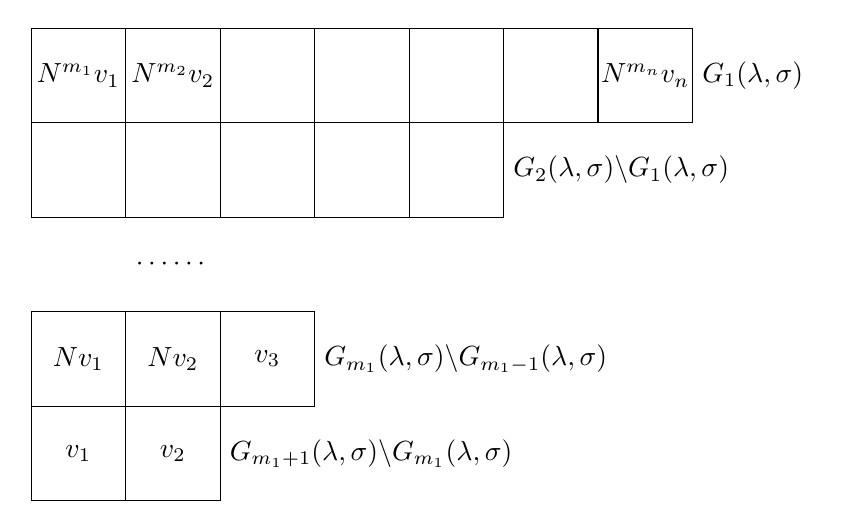
\begin{tikzpicture}[scale=1.2]
                  \foreach[count=\i] \len in {7, 7, 5, 3, 3, 2}
                  \draw (0, -\i+1) -- (\len, -\i+1);

                  \foreach \i in {0, 1, 2}
                  \draw (\i, -3) -- (\i, -5);

                  \draw (3, -3) -- (3, -4);

                  \foreach \i in {0,...,5}
                  \draw (\i, 0) -- (\i, -2);

                  \foreach \i in {6, 7}
                  \draw (\i, 0) -- (\i, -1);

                  \foreach \i in {1, 2} {
                  \node at (\i-.5, -4.5) {$v_{\i}$};
                  \node at (\i-.5, -.5) {$N^{m_{\i}}v_{\i}$};
                  }
                  \foreach \i in {1, 2}
                  \node at (\i-.5, -3.5) {$Nv_{\i}$};

                  \node at (3-.5, -3.5) {$v_{3}$};
                  \node at (6.5, -.5) {$N^{m_n}v_n$};
                  \node at (1.5, -2.5) {$\cdots\cdots$};

                  \node[anchor=west] at (7, -.5) {$G_1(\lambda,\sigma)$};
                  \node[anchor=west] at (5, -1.5) {$G_2(\lambda,\sigma) \backslash G_1(\lambda,\sigma)$};
                  \node[anchor=west] at (3, -3.5) {$G_{m_1}(\lambda,\sigma) \backslash G_{m_1-1}(\lambda,\sigma)$};
                  \node[anchor=west] at (2, -4.5) {$G_{m_1+1}(\lambda,\sigma) \backslash G_{m_1}(\lambda,\sigma)$};
              \end{tikzpicture}
              \caption{将若当基排列成Young图形式}
              \label{fig:17:若当基Young图形式}
          \end{figure}

    \item 接下来要确定每个若当循环基的长度,也就是Young图每一列的长度,我们应当从行的性质入手,因为这是我们目前仅有的可以计算的信息. 我们需要求解每个$G_j(\lambda,\sigma)$及其维数(目前只有维数有用,但后续求解具体若当基时其中的向量也是有用的),直到某个$G_j(\lambda,\sigma)$的维数等于$G_\lambda$的维数,因为Young图中所有方格与$G_\lambda$的一组基一一对应,因此方格总数就等于$G_\lambda$的维数. 另一方面由\autoref{thm:广义特征性质},$N$是$G_\lambda$上的幂零线性变换,且在其它广义特征子空间上是双射,因此在核空间最高次数也只能是$G_\lambda$的维数.

          在求出各个$G_j(\lambda,\sigma)$的维数后阶梯形状也即确定,因为各层向量个数确定了. 举个简单的例子,假设$G_\lambda$是11维空间,满足$G_1(\lambda,\sigma)$,$G_2(\lambda,\sigma)$,$G_3(\lambda,\sigma)$的维数分别为5,9,11. 对照Young图每行右侧的标注,这说明从最上方一行往下的向量个数依次为5,4($=9-5$),2($=11-9$),具体Young图为
          \begin{figure}[H]
              \centering
              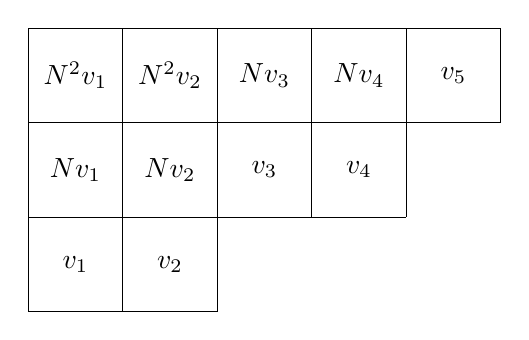
\begin{tikzpicture}[scale=1.2]
                  \foreach[count=\i] \len in {5, 5, 4, 2}
                  \draw (0, -\i+1) -- (\len, -\i+1);

                  \foreach \i in {0,...,5}
                  \draw (\i, 0) -- (\i, -1);
                  \foreach \i in {0,...,4}
                  \draw (\i, -1) -- (\i, -2);
                  \foreach \i in {0, 1, 2}
                  \draw (\i, -2) -- (\i, -3);

                  \node at (.5, -.5) {$N^2v_1$};
                  \node at (1.5, -.5) {$N^2v_2$};
                  \node at (2.5, -.5) {$Nv_3$};
                  \node at (3.5, -.5) {$Nv_4$};
                  \node at (4.5, -.5) {$v_5$};
                  \node at (.5, -1.5) {$Nv_1$};
                  \node at (1.5, -1.5) {$Nv_2$};
                  \node at (2.5, -1.5) {$v_3$};
                  \node at (3.5, -1.5) {$v_4$};
                  \node at (.5, -2.5) {$v_1$};
                  \node at (1.5, -2.5) {$v_2$};
              \end{tikzpicture}
          \end{figure}
          然后我们就能得到每组若当循环基的长度,即每个若当块的阶数,分别为$3,3,2,2,1$.
\end{enumerate}

基于上面的求解过程,我们就可以得到一般性的Young图大小的决定公式如下:
\begin{theorem}{}{Young图行长度}
    令$r_j$表示Young图从上至下第$j$行的格数,则有(其中$N=\sigma-\lambda I$):
    \begin{enumerate}
        \item $r_1=\dim V-r(N)$;
        \item $r_j=r(N)^{j-1}-r(N)^j(j>1)$.
    \end{enumerate}
\end{theorem}
\begin{proof}
    根据\autoref{fig:17:若当基Young图形式} 中每行右侧的标注的含义,第一行的格数就是$G_1(\lambda,\sigma)$的维数,即特征子空间的维数,即$\dim V-r(N)$;第$j(j>1)$行的格数就是$G_j(\lambda,\sigma)$的维数减去$G_{j-1}(\lambda,\sigma)$的维数,由线性映射基本定理,$\dim G_j(\lambda,\sigma)=\dim G_\lambda-r(N)^j$,$\dim G_{j-1}(\lambda,\sigma)=\dim G_\lambda-r(N)^{j-1}$,因此第$j$行的格数就是$r(N)^{j-1}-r(N)^j$.
\end{proof}

基于上述定理,我们可以进一步得到每个特征值对应的若当块个数和每个若当块大小的公式. 进一步地,这些公式实际上就表明了若当标准形的唯一性,因为每个特征值对应的若当块的个数和大小都可以被如下公式唯一确定. 我们将这一定理总结如下:
\begin{theorem}{}{若当标准形唯一}
    设$V$是$n$维复向量空间,$\sigma\in \mathcal{L}(V)$,$\lambda_1,\ldots,\lambda_m$为其互异的特征值,记$N_j=\sigma-\lambda_j I$,则主对角元为$\lambda_j$的若当块的个数$n_j$为
    \begin{equation} \label{eq:17:若当块个数}
        n_j=n-r(N_j),
    \end{equation}
    其中$t$级若当块$J_t(\lambda_j)$的个数$n_j(t)$为
    \begin{equation} \label{eq:17:若当块大小}
        n_j(t)=r(N_j^{t+1})+r(N_j^{t-1})-2r(N_j^t),
    \end{equation}
    以上公式表明,除若当块的排列次序外,一个线性变换对应的若当标准形唯一.
\end{theorem}
\begin{proof}
    实际上,证明这一定理就是要从\autoref{thm:Young图行长度} 中得到的Young图每行的长度推出Young图有多少列,以及每列的长度. 很显然,Young图的列数就是第一行的长度,即$\dim V-r(N_j)$. 进一步观察,我们知道Young图第$j$行与第$j+1$行的长度之差来源于有$r_j-r_{j+1}$(记号来源于\autoref{thm:Young图行长度})组循环若当基长度终止于$j$,因此大小为$j$的若当块的个数就是$r_j-r_{j+1}=r(N_j)^{t+1}+r(N_j)^{t-1}-2r(N_j)^t$.
\end{proof}

尽管我们理论上可以通过上述过程得到任意复向量空间上的线性变换的若当块的个数和大小,但我们知道,直接对线性变换计算特征值是困难的,因此更多的时候我们仍然是利用线性变换和它的矩阵表示的特征值与广义特征向量的对应关系,将求解线性变换的若当标准形转化为求解其某个矩阵表示的若当标准形.

于是我们讨论矩阵的情况. 我们考虑$P^{-1}AP=J$,其中$P$为过渡矩阵,$J$为$A$的若当标准形. 我们可以将$A$视为$\sigma(\alpha)=A\alpha$在自然基下的矩阵,于是$\sigma$在\autoref{cor:若当基存在} 给出的基(记为$B$)下的表示矩阵的求解方式就是$\sigma(B)=(B)J$,将$B$组成的矩阵记作$P$,代入$\sigma$的定义,$\sigma(B)=(B)J$就等同于$AP=PJ$,即$P^{-1}AP=J$,故如果我们要求矩阵相似于其若当标准形的过渡矩阵,问题转化为求解$\sigma(\alpha)=A\alpha$的若当基然后排列成矩阵即可.

然而我们知道,求解$\sigma$的若当基需要求解各个$G_i(\lambda,\sigma)=\ker(\sigma-\lambda I)^i$,代入$\sigma(\alpha)=A\alpha$可知,$G_i(\lambda,\sigma)$实际上就是$(A-\lambda I)^iX=0$的解. 所以对于矩阵而言,上述所有的过程都只是不断对矩阵求幂然后解线性方程组,因此是一定可解的. 我们用解空间替代各个$G_i(\lambda,\sigma)$重复上述过程可以得到如下定理:
\begin{theorem}{}{}
    设$A$是$n$阶复矩阵,$\lambda_1,\ldots,\lambda_m$为其互异的特征值,则主对角元为$\lambda_j$的若当块的个数$n_j$为
    \begin{equation} \label{eq:17:矩阵若当块个数}
        n_j=n-r(A-\lambda_j I),
    \end{equation}
    其中$t$级若当块$J_t(\lambda_j)$的个数$n_j(t)$为
    \begin{equation} \label{eq:17:矩阵若当块大小}
        n_j(t)=r(A-\lambda_j I)^{t+1}+r(A-\lambda_j I)^{t-1}-2r(A-\lambda_j I)^t,
    \end{equation}
    以上公式表明,除若当块的排列次序外,一个矩阵对应的若当标准形唯一.
\end{theorem}

最后我们需要提到一点,根据上面的叙述,若当标准形在不考虑若当块的排列顺序的情况下是唯一的. 因此任一复数域上矩阵均有唯一的若当标准形(相似标准形),因此我们可以知道,两矩阵相似的一个充要条件是两矩阵有相同的若当标准形(不考虑若当块的排列顺序),这也是判定两个矩阵是否相似的关键,当然之后我们还会学到其它判定方式,届时我们再做总结.

接下来我们将讨论如何求出Young图中所有方格中的向量,当然实际上只需确定每个终止向量即可得到所有向量. 在正式讨论之前,我们先考虑一种投机取巧的方式. 事实上,如果题目只要求我们求解矩阵的若当标准形时,如果我们要求解过渡矩阵,也有简单的方法. 要求$P$使得$P^{-1}AP=J$,则有$AP=PJ$. 假定$P$为$n$阶矩阵,我们可以设$P=(X_1,\ldots,X_n)$,剩下的任务就是解方程了. 因此这种方法非常简单,缺陷在于绕开了若当基这一本质的问题.
\begin{example}{}{}
    利用上述方法求解矩阵\[\begin{pmatrix}
            2 & 3 & 2 \\ 1 & 8 & 2 \\ -2 & -14 & -3
        \end{pmatrix}\]的若当标准形以及对应的过渡矩阵.
\end{example}

\begin{solution}

\end{solution}

下面我们将讨论对于一般的线性变换,无法投机取巧时,或者希望从更本质的角度求解时,我们应当使用的方法.

\begin{center}
    \textbf{\heiti 第二步\quad 求解 $\boldsymbol{v_1,\ldots,v_n}$}
\end{center}

\begin{enumerate}
    \item 实际上,我们在前述求解若当块大小的过程中求出了各个$G_j(\lambda,\sigma)$,接下来我们需要利用这些向量将之前确定形状的阶梯内容填满. 我们首先将阶梯最上方的向量确定,实际上就是利用求出的$G_{m_1+1}(\lambda,\sigma)$(也就是$V$)和$G_{m_1}(\lambda,\sigma)$求出二者之差. 似乎很简单,但若仔细思索便会发现线性空间的差并不一定好求. 举一个简单的例子,设$G_{m_1+1}(\lambda,\sigma)=\{\alpha_1,\alpha_2,\alpha_3,\alpha_4\}$,$G_{m_1}(\lambda,\sigma)=\{\beta_1,\beta_2\}$. 这其中出现的所有向量可能都完全不一样,所以作差并不容易. 但我们有一种好方法,如果我们每次从$G_{m_1+1}(\lambda,\sigma)$中挑选两个向量和$G_{m_1}(\lambda,\sigma)$中的两个向量放在一起,如果这四个向量线性无关,这就说明这两个挑出的向量就是作差的结果. 原因在于这相当于$G_{m_1}(\lambda,\sigma)$直和这两个向量长成的空间后得到了$G_{m_1+1}(\lambda,\sigma)$. 如果四个向量线性相关,这说明挑选的向量有在$G_{m_1}(\lambda,\sigma)$中的.

    \item 接下来继续计算第二行中的向量. 实际上算出第一行后第二行中部分向量就已经确定了,例如图上的$Nv_1$和$Nv_2$. 我们这时用类似的方法求解$G_{m_1}(\lambda,\sigma)$和$G_{m_1-1}(\lambda,\sigma)$的差,如图只需要确定一个向量,但这一个向量的确定除了要像(a)中一样每次从$G_{m_1}(\lambda,\sigma)$中选择一个与$G_{m_1-1}(\lambda,\sigma)$的基一起判断线性相关性外,还需要确保这个向量和已经求出的$Nv_1$和$Nv_2$是线性无关的,因为它们构成$G_{m_1}(\lambda,\sigma)$的一组基.

          总结一下,处于$G_j(\lambda,\sigma)\backslash G_{j-1}(\lambda,\sigma)$对应的行的需要补充的向量$v$应当满足如下三个条件:
          \begin{enumerate}
              \item $v\in G_j(\lambda,\sigma)$;

              \item $v\notin G_{j-1}(\lambda,\sigma)$(通过加入$G_{j-1}(\lambda,\sigma)$)的基保证线性无关判断);

              \item $v$与同一行中左边已求出的向量线性无关.
          \end{enumerate}

    \item 最后,我们将所有求出的基按照若当基原先的排列顺序重新组合即可. 如果求矩阵相似于若当标准形的过渡矩阵,则按顺序按列摆放即可.
\end{enumerate}

我们可以通过一个例子来说明上述过程.
\begin{example}{}{}
    设$V$是由两个变量$x,y$生成的次数不大于2的多项式函数(例如$xy^2$不是,因为次数等于1+2=3,$x^2+y$是)关于一般的多项式加法和数乘构成的线性空间,于是我们可以取一组基为$\{1,x,y,x^2,y^2,xy\}$,定义$\sigma\in \mathcal{L}(V)$为
    \[\sigma(f(x,y))=\dfrac{\partial}{\partial x}f(x,y).\]
    求$V$的一组基使得$\sigma$在这组基下的矩阵是若当标准形.
\end{example}
\begin{solution}

\end{solution}

\section{若当标准形的应用}
\subsection{求解不变子空间}
在不变子空间一节中我们提到,我们可以利用若当标准形求解不变子空间. 下面是一个与若当块直接相关的例子:
\begin{example}{}{}
    设$V$为$n$维复向量空间,$\sigma\in \mathcal{L}(V)$,$\sigma$在基$v_1,\ldots,v_n$下的矩阵是一个若当块
    \[\begin{pmatrix}
            \lambda & 1       & 0      & \cdots & 0       \\
            0       & \lambda & 1      & \cdots & 0       \\
            \vdots  & \vdots  & \vdots & \ddots & \vdots  \\
            0       & 0       & 0      & \cdots & \lambda
        \end{pmatrix},\]
    证明:
    \begin{enumerate}
        \item $V$中包含$v_n$的不变子空间只有$V$自身;

        \item $V$中任意非零不变子空间都包含$v_1$;

        \item $V$不能分解为两个非平凡的不变子空间的直和;

        \item $V$中有且仅有$n+1$个不变子空间,它们分别是
              \[\{0\},\spa(v_1),\spa(v_1,v_2),\ldots,\spa(v_1,\ldots,v_{n-1},v_n)\]
    \end{enumerate}
\end{example}

\begin{solution}
    \begin{enumerate}
        \item 设$W$是包含$v_n$的不变子空间,根据线性映射矩阵表示的定义,$\sigma(v_n)=\lambda v_n+v_{n-1}\in W$,故$v_{n-1}\in W$,同理可得$v_{n-2},\ldots,v_1\in W$,即$W=V$.

        \item 设$U$为任一非零不变子空间,那么$U$中存在一个非零向量$v$,则$v$一定可以表达为
              \[v=k_1v_1+\cdots+k_sv_s(s\leqslant n),\]
              其中$k_s\neq 0$. 由$\sigma(v)\in U$以及线性映射矩阵表示有
              \begin{align*}
                  \sigma(v) & = \lambda k_1v_1+k_2(\lambda v_2+v_1)+\cdots+k_s(\lambda v_s+v_{s-1}) \\
                            & = \lambda v+k_2v_1+\cdots+k_sv_{s-1}\in U,
              \end{align*}
              因此$k_2v_1+\cdots+k_sv_{s-1}\in U$,同理进一步作用$\sigma$有$k_3v_1+\cdots+k_sv_{s-2}\in U$,以此类推有$k_sv_1\in U$. 又$k_s\neq 0$,故$v_1\in U$,命题得证.

        \item 利用上一点显然.

        \item 显然$\{0\},\spa(v_1),\spa(v_1,v_2),\ldots,\spa(v_1,\ldots,v_{n-1},v_n)$都是不变子空间,下面证明不变子空间一定在它们当中.

              设$U$为任一不变子空间,若$U=\{0\}$,则也符合结论. 我们考虑非零的情况,设$\beta_1,\ldots,\beta_s$是$U$的一组基,并且假设
              \[\beta_i=a_{i1}v_1+a_{i2}v_2+\cdots+a_{it}v_t,\enspace i=1,2,\ldots,s\]
              其中满足至少有一个$i$使得$a_{it}\neq 0$(把所有基下表示末尾的0去除即可). 对于满足$a_{it}\neq 0$的$i$,由于$U$是不变子空间,故$\sigma(\beta_i)\in U$,与第二点证明完全相同,我们得到
              \begin{align*}
                  a_{i2}v_1+a_{i3}v_2+\cdots+a_{it}v_{t-1}\in U, \\
                  a_{i3}v_1+a_{i4}v_2+\cdots+a_{it}v_{t-2}\in U, \\
                  \cdots                                         \\
                  a_{i,t-1}v_1+a_{it}v_2\in U,                   \\
                  a_{it}v_1\in U.
              \end{align*}
              由于$a_{it}\neq 0$,故由最后的式子知道$v_1\in U$. 代入倒数第二个式子知道$v_2\in U$,以此类推,最终得到$\spa(v_1,\ldots,v_t)\subset U$,而$U\subset\spa(v_1,\ldots,v_t)$显然(因为每个$\beta_i$都在其中),故命题得证.
    \end{enumerate}
\end{solution}

因此我们如果能将线性变换在一组基下表示为若当块,我们就可以很快地利用这一例子的结论写出其不变子空间. 但我们有时候会遇到线性变换在一组基下表示为多个若当块的情况,这时我们可能需要通过组合不同若当块对应的不变子空间来得到线性变换的不变子空间(很容易知道不相交的不变子空间的直和还是不变子空间,因为矩阵表示还是分块对角矩阵),并且同时还要证明组合出来的就是全部的不变子空间. 下面就是一个非常经典的例子:
\begin{example}{}{}
    设$V$是复数域上的$n$维线性空间,$\sigma\in\mathcal{L}(V)$,若$\sigma$有$n$个不同的特征值$\lambda_1,\ldots,\lambda_n$,求$\sigma$的不变子空间的个数.
\end{example}
\begin{solution}
    显然$\sigma$可对角化,每个对角元素就是一阶若当块,因此我们需要考虑组合这些若当块对应的基构成新的不变子空间. 由可对角化我们有
    \[V=V_{\lambda_1}\oplus\cdots\oplus V_{\lambda_n},\]
    结合$\dim V=n$可知每个特征子空间都是1维的. 根据我们组合的思想,我们知道对于任意的$1\leqslant j_1<j_2<\cdots<j_r\leqslant n$,$r=1,2,\ldots,n$,$V_{\lambda_{j_1}}\oplus\cdots\oplus V_{\lambda_{j_r}}$都是不变子空间. 这样的不变子空间加上零空间的个数总和为$\mathrm{C}_n^0+\mathrm{C}_n^1+\cdots+\mathrm{C}_n^n=2^n$.

    下面我们需要说明这些不变子空间是全部的不变子空间. 设$U$为任一不变子空间,若为零空间则符合要求,若不是零空间,设$\dim U=m>0$,$U$的一组基为$\beta_1,\ldots,\beta_m$,将其扩充为$V$的一组基$\beta_1,\ldots,\beta_m,\beta_{m+1},\ldots,\beta_n$,则在这组基下$\sigma$的矩阵为
    \[B=\begin{pmatrix}
            A & C \\ O & D
        \end{pmatrix},\]
    于是$\sigma\vert_W$的矩阵为$A$,对应特征多项式$|\lambda E-A|$可以整除$\sigma$的特征多项式$|\lambda E-B|=|\lambda E-A||\lambda E-D|$,由于$\sigma$有$n$个不同的特征值,因此$\sigma\vert_W$必定有$m$个不同的特征值$\lambda_{l_1},\ldots,\lambda_{l_m}$,且$1\leqslant l_1<\cdots<l_m\leqslant n$,而对每个特征值$\lambda_{l_i}$都有特征向量$\alpha_i\in W$,满足$\sigma\vert_W(\alpha_i)=\lambda_{l_i}\alpha_i$,因此$\sigma(\alpha)=\lambda_{l_i}\alpha_i$,即$\alpha_i\in V_{\lambda_{l_i}}$,故$V_{\lambda_{l_1}}\oplus\cdots\oplus V_{\lambda_{l_m}}\subset U$. 再结合
    \[\dim(V_{\lambda_{l_1}}\oplus\cdots\oplus V_{\lambda_{l_m}})=m=\dim U,\]
    故$U=V_{\lambda_{l_1}}\oplus\cdots\oplus V_{\lambda_{l_m}}$,故所有不变子空间都是之前讨论的$2^n$种之一,命题得证.
\end{solution}

当然需要注意的是,不变子空间的个数不一定有限,例如对于数乘变换$\sigma=kI\in\mathcal{L}(V)$,很容易验证$V$的任意子空间都是其不变子空间.

\subsection{矩阵求幂与马尔可夫链}

若当标准形的另一个应用在于我们可以利用它计算矩阵的幂,因为若当块的幂的计算是简单的,这一点与对角矩阵是类似的:
\[J_k(a)^n=(aE+J_k(0))^n=a^nE+\mathrm{C}_n^1a^{n-1}J_k(0)+\cdots+\mathrm{C}_n^nJ_k(0)^n\]
同时我们也知道$J_k(0)^k=O$(幂零矩阵),所以利用若当标准形求解矩阵的幂是简单的. 我们来看一个例子:
\begin{example}{}{}
    设$A=\begin{pmatrix}
            2 & 6 & -15 \\ 1 & 1 & -5 \\ 1 & 2 & -6
        \end{pmatrix}$,求$A^{m}(m\geqslant 1)$.
\end{example}
\begin{solution}

\end{solution}

下面是一个非常经典的例子,在接下来的讨论中还会有应用:
\begin{example}{}{若当m次幂}
    设$J=J_n(a)$是特征值为$a$的$n$阶若当块,求$J^m$的若当标准形,其中$m$为非零整数.
\end{example}
\begin{solution}
    我们需要分别考虑$a\neq 0$和$a=0$的情况:
    \begin{enumerate}
        \item 当$a\neq 0$时,首先显然$J^m$的特征值都为$a^m$,我们先处理$m\geqslant 1$的情况,我们有
              \[J^m=(aE+J(0))^m=a^mE+\mathrm{C}_m^1a^{m-1}J_n(0)+\cdots+\mathrm{C}_m^mJ_n(0)^m.\]
              故$r(J^m-a^mE_n)=r(\mathrm{C}_m^1a^{m-1}J_n(0)+\cdots+\mathrm{C}_m^mJ_n(0)^m)=n-1$(很容易通过$J_n(0)$的幂次的特点写出这一矩阵,然后通过行列式秩判断),因此根据\autoref{thm:若当标准形唯一} 可知$J^m$的若当块个数为$n-(n-1)=1$,因此$J^m$的若当标准形就是$J_n(a^m)$.

              然后我们考虑$m=-1$的情况,显然$J^{-1}$的特征值为$a^{-1}$,这里我们借用\autoref{ex:分式求逆1} 的分式思想,得到
              \[J^{-1}=\dfrac{1}{a}E_n-\dfrac{1}{a^2}J_n(0)+\cdots+(-1)^{n-1}\dfrac{1}{a^n}J_n(0)^{n-1}.\]
              故$r(J^{-1}-\dfrac{1}{a}E_n)=r(-\dfrac{1}{a^2}J_n(0)+\cdots+(-1)^{n-1}\dfrac{1}{a^n}J_n(0)^{n-1})=n-1$,因此$J^{-1}$的若当块个数为$n-(n-1)=1$,因此$J^{-1}$的若当标准形就是$J_n(a^{-1})$.

              最后处理$m\leqslant -2$的情况,注意到$J^m=(J_n^{-1})^{-m}$,故根据前面$m\geqslant 1$的讨论,$J^m$的若当标准形就是$J_n((a^{-1})^{-m})=J_n(a^m)$.

              综上所述,无论$m$取什么整数值,$J^m$的若当标准形就是$J_n(a^m)$.

        \item 当$a=0$时,我们有$m\geqslant n$时$J^m=O$,此时若当标准形也就是零矩阵. 我们考虑$m<n$的情况,我们需要使用\autoref{thm:若当标准形唯一} 的结论来辅助我们求解$J^m$的若当标准形,因此我们需要研究$(J^m)^k$的秩. 我们做带余除法,$n=mq+r(0\leqslant r<m)$,则根据$J_n(0)$的幂次的特点,我们有
              \[r((J^m)^k)=n-mk,\enspace 0\leqslant k\leqslant q,\enspace r((J^m)^k)=0,\enspace k\geqslant q+1.\]
              因此
              \begin{enumerate}
                  \item $1\leqslant k<q$时,$J_k(0)$的个数为$r((J^m)^{k-1})+r((J^m)^{k+1})-2r((J^m)^k)=(n-m(k-1))+(n-m(k+1))-2(n-mk)=0$;
                  \item $k=q$时,$J_k(0)$的个数为$r((J^m)^{q-1})+r((J^m)^{q+1})-2r((J^m)^q)=(n-m(q-1))+0-2(n-mq)=m-r$;
                  \item $k=q+1$时,$J_k(0)$的个数为$r((J^m)^q)+r((J^m)^{q+2})-2r((J^m)^{q+1})=(n-mq)+0-0=r$.
                  \item $k>q+1$时,$J_k(0)$的个数为0.
              \end{enumerate}
              综上所述,$J^m$的若当标准形是$\diag(J_q(0),\ldots,J_q(0),J_{q+1}(0),\ldots,J_{q+1}(0))$,其中$J_q(0)$的个数为$m-r$,$J_{q+1}(0)$的个数为$r$.
    \end{enumerate}
\end{solution}

由于复数域上任意矩阵都有若当标准形,因此利用若当标准形,我们可以求出复数域上任意矩阵的任意幂次. 于是我们会有一个问题,即任意给定一个矩阵,当我们取其幂次趋向于无穷时,会得到一个什么样的矩阵呢?是所有元素都有限的矩阵,还是有些元素可能趋于无穷了呢?

\subsection{若当标准形与矩阵分解}
矩阵分解是我们讨论标准形时绕不开的话题,接下来我们讨论若当标准形应用于矩阵分解的情形. 我们首先讨论平方根分解,这一点是之前线性变换平方根讨论的延续. 下面这一结论是相当经典的:
\begin{theorem}{}{若当标准形m次根}
    在复数域上,我们有如下关于若当标准形的根式结论:
    \begin{enumerate}
        \item 设$a\neq 0$,则存在矩阵$A$使得$A^m=J_n(a)$;
        \item 当$n\geqslant 2$时,不存在矩阵$A$使得$A^m=J_n(0)$.
    \end{enumerate}
\end{theorem}

\begin{proof}
    \begin{enumerate}
        \item 根据\autoref{ex:若当m次幂},我们知道$J_n(a)^m\sim J_n(a^m)$. 设$b^m=a$(在复数域上一定存在这样的$b$),则$J_n(b)^m\sim J_n(a)$,因此存在可逆矩阵$P$使得$P^{-1}J_n(b)^mP=J_n(a)$,取$A=P^{-1}J_n(b)P$即可.

        \item 反证法. 若存在矩阵$A$使得$A^m=J_n(0)$,则$A$显然也为$n$阶幂零矩阵,因此有$A^n=O$(因此至少有$m\leqslant n$). 设$n=mq-r(m\geqslant 2,0\leqslant r<m)$,则$O=A^{n+r}=(A^m)^q=J_n(0)^q\neq O$,这是因为$J_n(0)$至少需要$n$次才能化零,但$n=mq-r(m\geqslant 2,0\leqslant r<m)$表明$q<n$,故矛盾.
    \end{enumerate}
\end{proof}

接下来我们考虑之前已经证明的\autoref{thm:幂零平方根} 的\ref*{item:16:幂零平方根:2},即可逆线性变换一定有平方根,我们现在可以使用若当标准形的方式证明. 我们直接使用矩阵证明即可,因为基固定的情况下矩阵和线性映射一一对应. 因为可逆线性变换对应可逆矩阵$A$,可逆矩阵特征值均不为0,因此每个对应的若当标准形$J$的若当块对角线上都不为0,均有平方根(即上述定理中$m=2$,我们记$B^2=J$). 进一步地,由于一定存在可逆矩阵$P$使得$P^{-1}AP=J$,我们取$C=PBP^{-1}$,则$C^2=PB^2P^{-1}=PJP^{-1}=A$,故我们找到了任意可逆矩阵对应的平方根$C$. 这一结论显然可以进一步推广,即任意复数域上的可逆线性变换和可逆矩阵一定有$m$次方根.

利用若当标准形,我们还可以有以下著名的Jordan-Chevalley分解. 这一定理的证明过程将会给出我们利用若当标准形证明一般矩阵性质的通用方法,一般包含如下步骤:
\begin{enumerate}
    \item 证明结论对于若当块成立;
    \item 证明结论对于若当标准形成立;
    \item 利用问题在相似下的不变性证明结论对于一般矩阵成立.
\end{enumerate}

事实上,上面讨论任意复可逆矩阵均有平方根也是遵循这一范式证明的,我们也是先证明了对角线元素非零的若当块一定有平方根,那么自然若当标准形是由若当块构成的分块对角矩阵也满足这一性质,然后利用$(P^{-1}AP)^n=P^{-1}A^nP$这一相似具有的运算特点证明对一般可逆矩阵有平方根成立. 总而言之,当我们希望使用若当标准形证明矩阵具有的性质时,这些性质在相似下要有一定的不变性,然后我们遵照上述范式即可给出证明. 因此,我们发现了研究相似标准形的一个重要的意义,因为这些很简单的矩阵一般而言都是具有很好的性质的,再结合很多性质在相似下都可以保持,因此我们可以通过研究更容易处理的相似标准形来研究一般矩阵的性质. 下面我们就开始证明这一著名的分解:

\begin{theorem}{Jordan-Chevalley分解}{}
    设$A$是$n$阶复矩阵,则$A$可分解为$A=B+C$,其中$B,C$满足如下条件:
    \begin{enumerate}
        \item $B$是可对角化的;
        \item $C$是幂零的;
        \item $BC=CB$;
        \item $B,C$均可以表示为$A$的多项式.
    \end{enumerate}
    不仅如此,满足上述条件1-3的分解是唯一的.
\end{theorem}

\begin{proof}
    我们首先对若当块$J_n(a)$证明这一定理. 事实上这非常显然,我们取$B=aE_n$,$C=J_n(0)$,则$B$可对角化,$C$是幂零的,且$BC=CB=aJ_n(0)$. 又因为$O=C^n=(J_n(a)-B)^n$,因此我们取$f(x)=(x-a)^n+a$,代入$x=J_n(a)$有
    $f(J_n(a))=(J_n(a)-aE_n)^n+aE_n=aE_n=B$,因此$B$表示为了$A$的多项式,而$C=J_n(a)-B=J_n(a)-f(J_n(a))$也是$A$的多项式.

    接下来推广到若当标准形$J$,我们假设$J$互不相同的特征值为$\lambda_1,\ldots,\lambda_m$,设每个特征值$\lambda_i$对应$s_i$个若当块,则可以将$J$表示为
    \[J=\begin{pmatrix}
            J_{11} &        &          &        &        &        &          \\
                   & \ddots &          &        &        &        &          \\
                   &        & J_{1s_1} &        &        &        &          \\
                   &        &          & \ddots &        &        &          \\
                   &        &          &        & J_{m1} &        &          \\
                   &        &          &        &        & \ddots &          \\
                   &        &          &        &        &        & J_{ms_m}
        \end{pmatrix}.\]
    对每个若当块$J_{ij}$,假设若当块大小为$k_{ij}$,我们类似于前面对若当块的讨论取出每个$M_{ij}=\lambda_i E_{k_{ij}}$,$N_{ij}=J_{k_{ij}}(0)$,然后将这些矩阵按$J$的顺序排列成分块对角矩阵即可得到$M$和$N$,则$J=M+N$,$M$可对角化,$N$是幂零的,且$MN=NM$是容易验证的.

    我们设每个特征值$\lambda_i$对应的最大的若当块的阶数为$k_i$,因此$(J_{ij}-\lambda_{ij})^{k_i}=O$. 我们知道$(\lambda-\lambda_1)^{k_1},\ldots,(\lambda-\lambda_m)^{k_m}$是两两互素的多项式,因此由\nameref{thm:中国剩余定理}可知,存在多项式$f(\lambda)$满足
    \[f(\lambda)=g_i(\lambda)(\lambda-\lambda_i)^{k_i}+\lambda_i,\enspace i=1,\ldots,m\]
    故$f(J_{ij})=g_i(J_{ij})(J_{ij}-\lambda_i)^{k_i}+\lambda_iE_{k_{ij}}=\lambda_iE_{k_{ij}}=M_{ij}$,因此$f(J)=M$也成立. 同理$N=J-M=J-f(J)$也是$J$的多项式,因此命题结论对若当标准形都成立.

    接下来考虑一般情形,设$P^{-1}AP=J$,则$A=PJP^{-1}=P(M+N)P^{-1}=PMP^{-1}+PNP^{-1}$. 取$B=PMP^{-1}$,$C=PNP^{-1}$,则$B$可对角化,$C$是幂零的,且$BC=CB$,$B,C$均可以表示为$A$的多项式都可以从$M,N$具有这样的性质立刻得到,即这一问题是在相似下不变的.

    最后证明唯一性. 假设$A$有另一满足1-3的分解$A=B'+C'$,则$B-B'=C'-C$,由$B'C'=C'B'$,结合$A=B'+C'$可知$AB'=B'A,AC'=C'A$,又因为$B=f(A)$,故$BB'=B'B$,同理有$CC'=C'C$. 设$C^r=O,C'^t=O$,用二项式定理可知$(C-C')^{r+t}=O$,因此$(B-B')^{r+t}=O$.

    我们知道$B$和$B'$可对角化且$BB'=B'B$,根据上一讲的习题可知它们可以同时对角化,即存在可逆矩阵$Q$使得$Q^{-1}BQ$和$Q^{-1}B'Q$均为对角矩阵. 注意到
    \[(Q^{-1}BQ-Q^{-1}B'Q)^{r+t}=(Q^{-1}(B-B')Q)^{r+t}=Q^{-1}(B-B')^{r+t}Q=O,\]
    又两对角矩阵的差是对角矩阵,因此只能有$Q^{-1}BQ=Q^{-1}B'Q$,即$B=B'$,从而$C=C'$也成立,因此唯一性得证.
\end{proof}

\subsection{求解微分方程}

取一常系数微分方程如下:
\[\dfrac{\mathrm{d}f_1}{\mathrm{d}x^2}-a\dfrac{\mathrm{d}f_1}{\mathrm{d}x}=bf_1.\]
令$\dfrac{\mathrm{d}f_1}{\mathrm{d}x}=f_2$,则上式可以改写为
\[\begin{cases}
        \dfrac{\mathrm{d}f_1}{\mathrm{d}x}=f_2, \\
        \dfrac{\mathrm{d}f_2}{\mathrm{d}x}=af_2+bf_1.
    \end{cases}\]
我们可以将上述方程写成矩阵形式:
\[\dfrac{\mathrm{d}}{\mathrm{d}x}\begin{pmatrix}
        f_1 \\ f_2
    \end{pmatrix}=\begin{pmatrix}
        0 & 1 \\ b & a
    \end{pmatrix}\begin{pmatrix}
        f_1 \\ f_2
    \end{pmatrix}.\]

类似地,$n$阶常微分方程
\[\dfrac{\mathrm{d}f_1}{\mathrm{d}x^n}-a_{n-1}\dfrac{\mathrm{d}f_1}{\mathrm{d}x^{n-1}}-\cdots-a_1\dfrac{\mathrm{d}f_1}{\mathrm{d}x}=bf_1\]
可以改写为
\[\dfrac{\mathrm{d}}{\mathrm{d}x}\begin{pmatrix}
        f_1 \\ f_2 \\ \vdots \\ f_n
    \end{pmatrix}=\begin{pmatrix}
        0      & 1      & 0      & \cdots & 0       \\
        0      & 0      & 1      & \cdots & 0       \\
        \vdots & \vdots & \vdots & \ddots & \vdots  \\
        0      & 0      & 0      & \cdots & 1       \\
        b      & a_1    & a_2    & \cdots & a_{n-1}
    \end{pmatrix}\begin{pmatrix}
        f_1 \\ f_2 \\ \vdots \\ f_n
    \end{pmatrix}=C\begin{pmatrix}
        f_1 \\ f_2 \\ \vdots \\ f_n
    \end{pmatrix}.\]
若有$P^{-1}CP=J$,令
\[P^{-1}\begin{pmatrix}
        f_1 \\ f_2 \\ \vdots \\ f_n
    \end{pmatrix}=\begin{pmatrix}
        g_1 \\ g_2 \\ \vdots \\ g_n
    \end{pmatrix},\]
于是我们有
\[\dfrac{\mathrm{d}}{\mathrm{d}x}\begin{pmatrix}
        g_1 \\ g_2 \\ \vdots \\ g_n
    \end{pmatrix}=J\begin{pmatrix}
        g_1 \\ g_2 \\ \vdots \\ g_n
    \end{pmatrix}.\]

一个直观的事情是$J$越简单方程越容易解,因此这时若当标准形就能帮助我们解决这一问题.

\subsection{求解线性递推方程}

数列的线性递推方程求解是我们高中就曾经接触过的问题,在行列式的运算技巧中我们也曾提及二阶齐次线性递推方程的求解,不过那种方法显然缺乏普适性. 很自然地,我们希望能寻求某种方法来解决$m$阶线性递推方程,不过在此之前,我们需要明确这其中蕴含的线性性究竟在何处.

让我们先从二阶开始,考虑$a_n = k_1 a_{n - 1} + k_2 a_{n - 2}$,显然其特征方程为$x^2 - k_1 x - k_2 = 0$,考虑无重根($\Delta = k_1 + 4k_2 \neq 0$)的情况,有$\lambda_1 = \dfrac{k_1 + \sqrt{k_1 + 4k_2}}{2}, \lambda_2 = \dfrac{k_1 - \sqrt{k_1 + 4k_2}}{2}$,且通项为$a_n = A \lambda_1^n + B \lambda_2^n$,其中$A, B$为待定常数. 而事实上,这个递推方程可以用一个线性映射去表示. 设$T \in \mathcal{L}(\mathbf{F}^2)$为$T(x_1, x_2) = (x_2, k_2 x_1 + k_1 x_2)$,则有$T(a_{n - 2}, a_{n - 1}) = (a_{n - 1}, a_n)$,便可以得到$T^n(a_0, a_1) = (a_n, a_{n + 1})$,也就是说,如果对初值进行$n$次线性变换,我们便可以得到第$n$项的值,但这个计算量过于庞大了. 而回忆我们先前处理算子的幂的方法,很快便能回想起相似标准型,所以接下来我们需要转向求出这一算子的特征值与特征向量.

考虑$T(x_1, x_2) = \lambda (x_1, x_2)$,得到方程组$\begin{cases} x_2 = \lambda x_1 \\ k_2 x_1 + k_1 x_2 = \lambda x_2 \end{cases}.$ 考虑到特征向量不为零向量,所以消去$x_1, x_2$后可以得到关于$\lambda$的方程$\lambda^2 - k_1 \lambda - k_2 = 0$,所以这个方程才会被称为特征方程,因为它的根是算子的特征值. 在没有重根的情况下,解得两个特征值为$\lambda_1, \lambda_2$,而对应的特征向量为$v_1 = (1, \lambda_1), v_2 = (1, \lambda_2)$. 我们知道对应不同特征值的特征向量是线性无关的,并且这里的数量正好等于空间维数,所以这两个特征向量构成了空间的一组基,且算子在这组基下的矩阵表示是简单的,为对角阵$\Lambda = \begin{pmatrix} \lambda_1 & 0 \\ 0 & \lambda_2 \end{pmatrix}$. 设$(a_0, a_1) = c_1 v_1 + c_2 v_2$,而使用矩阵求出坐标再代入基是计算量较小的,所以有 $\Lambda^n \begin{pmatrix}
        c_1 \\ c_2
    \end{pmatrix} = \begin{pmatrix}
        c_1 \lambda_1^n \\ c_2 \lambda_2^n
    \end{pmatrix}$,这便是$(a_n, a_{n + 1})$在这组基下的坐标,代入$v_1, v_2$即可得到通解$a_n = c_1 \lambda_1^n + c_2 \lambda_2^n$.

而对于$m$阶线性递推方程$a_n = k_1 a_{n - 1} + k_2 a_{n - 2} + \cdots + k_m a_{n - m}$,其无重根的情况是二阶的简单推广. 考虑$T \in \mathcal{L}(F^m)$,$T(x_1, x_2, \ldots, x_m) = (x_2, x_3, \ldots, k_m x_1 + k_{m - 1} x_2 + \cdots + k_1 x_m)$,则$T(a_{n - m}, a_{n - m + 1}, \ldots, a_{n - 1}) = (a_{n - m + 1}, a_{n - m + 2}, \ldots, a_n)$,对应的特征方程为$x^m - k_1 x^{m - 1} - \cdots - k_m = 0$,得到特征值为$\lambda_1, \lambda_2, \ldots, \lambda_m$,而对应的特征向量为$v_i = (1, \lambda_i, \lambda_i^2, \ldots, \lambda_i^{m - 1})$,通解为$a_n = \sum_{i = 1}^m c_i \lambda_i^n$. 另一个有趣的事实是所有的特征向量也能组成一个 Vandermonde 矩阵,这也可以从另一个侧面印证为什么要求没有重根.

那么如果存在重根又会发生什么情况呢?我们依然先以一个二阶线性递推方程为例,考虑$a_n = 2 \lambda_0 a_{n - 1} - \lambda_0^2 a_{n - 2}$,构造相应的算子$T(x_1, x_2) = (x_2, 2 \lambda_0 x_2 - \lambda_0^2 x_1)$,则$T(a_{n - 2}, a_{n - 1}) = (a_{n - 1}, a_n)$,特征值易求得为$\lambda_0$,对应特征向量为$(1, \lambda_0)$. 特征空间为一维的,显然不能够对角化,所以它应该对应为二阶的若当块的情况,已知$v_1 = (1, \lambda_0)$,求出满足$(T - \lambda_0 I)v_2 = v_1$的$v_2$即求出了若当基. 满足条件的一个$v_2 = (0, 1)$,在这组基下$T$的矩阵表示为$\begin{pmatrix} \lambda_0 & 1 \\ 0 & \lambda_0 \end{pmatrix} = \lambda_0 I + J$,其中$J = \begin{pmatrix} 0 & 1 \\ 0 & 0 \end{pmatrix}$ 且 $J^2 = O$. 设$(a_0, a_1) = c_1v_1 + c_2v_2$,那么有
\begin{align*}
    M^n \begin{pmatrix} c_1 \\ c_2 \end{pmatrix}
     & = (\lambda_0 I + J)^n \begin{pmatrix} c_1 \\ c_2 \end{pmatrix}                                                          \\
     & = (\lambda^n I + n \lambda^{n - 1} J) \begin{pmatrix} c_1 \\ c_2 \end{pmatrix}                                          \\
     & = \begin{pmatrix} \lambda^n & n \lambda^{n - 1} \\ 0 & \lambda^n \end{pmatrix} \begin{pmatrix} c_1 \\ c_2 \end{pmatrix} \\
     & = \begin{pmatrix} c_1 \lambda^n + n c_2 \lambda^{n - 1} \\ d \lambda^n \end{pmatrix}.
\end{align*}
从而代入$v_1, v_2$有$a_n = c_1 \lambda_0^n + n c_2 \lambda_0^{n - 1}$.

进而我们可以考虑一个$m$阶线性递推方程,且其特征方程有$m$重根$\lambda_0 \neq 0$的情况(特征值为$0$是退化的),这时对应的是一个$m$阶的若当块,重点在于求出其对应的若当基. 首先对应的算子$T$的形式应当为$T(x_1, x_2, \ldots, x_m) = (x_2, x_3, \ldots, (-1)^{m + 1} \binom{m}{0} \lambda_0^m x_1 + (-1)^m \binom{m}{1} \lambda_0^{m - 1} x_2 + \cdots + (-1)^2 \binom{m}{m - 1} \lambda_0 x_{m})$,要求出特征向量即求出满足$(T - \lambda_0 I)v_1 = 0$的$v_1$,这一线性方程组的系数矩阵如下:
\[
    \begin{pmatrix}
        -\lambda_0                            & 1                                     & 0                                           & \cdots & 0                                       \\
        0                                     & -\lambda_0                            & 1                                           & \cdots & 0                                       \\
        \vdots                                & \vdots                                & \vdots                                      & \ddots & \vdots                                  \\
        0                                     & 0                                     & 0                                           & \cdots & 1                                       \\
        (-1)^{m + 1} \binom{m}{0} \lambda_0^m & (-1)^m \binom{m}{1} \lambda_0^{m - 1} & (-1)^{m - 1} \binom{m}{2} \lambda_0^{m - 2} & \cdots & ((-1)^2 \binom{m}{m - 1} - 1) \lambda_0
    \end{pmatrix}
\]
我们能轻松得到$v_1 = (\lambda_0^0, \lambda_0, \lambda_0^2, \ldots, \lambda_0^{m - 1})$是满足前$m-1$行的,代入验证也满足第$m$行. 因为前$m-1$行是线性无关的,所以我们基本上可以宣称第$m$行是前$m-1$行的线性组合,也就是说这个矩阵的秩为$m-1$. 但是,这个线性组合的系数在后续求解若当基的过程中相当重要,所以我们还是要求出来. 记以上系数矩阵为$\begin{pmatrix}
        \beta_1 \\ \beta_2 \\ \vdots \\ \beta_m
    \end{pmatrix}$,$\beta_i$均是行向量. 这个系数求解的关键在于第$2$到第$m-1$个坐标都是有两个行向量来控制的,并且$\beta_m$每个是以组合数为基础的,我们能够很自然的联想到杨辉三角. 首先第$1$个坐标能够给出第一个系数$t_1 = (-1)^m \binom{m - 1}{0} \lambda_0^{m - 1}$,然后第$2$个坐标结合杨辉三角便可以得到$t_2 = (-1)^{m - 1} \binom{m - 1}{1} \lambda_0^{m - 2}$,以此类推,直到第$m-1$个坐标$t_{i - 1} = (-1)^2 \binom{m-1}{m-2} \lambda_0$. 第$m$个坐标我们需要验证其正确性,因为其减去了$1$所以形式上有所区别,但我们可以将其改写为$((-1)^2 \binom{m}{m - 1} - \binom{m - 1}{m - 1}) \lambda_0 = ((-1)^2 \binom{m - 1}{m - 2}) \lambda_0$,与$t_{i-1}$一致. 所以我们有 \[
    \beta_m = t_1 \beta_1 + t_2 \beta_2 + \cdots + t_{m - 1} \beta_{m - 1}.
\]
其中$t_i = (-1)^{m + 1 - i} \binom{m - 1}{i - 1} \lambda_0^{m - i}$.

因为$v_1$的求解是基于齐次线性方程组,所以系数的作用不是很明确. 但当我们开始求解$v_2, v_3, \ldots, v_m$时,这就意味着我们需要处理非齐次线性方程组,需要验证$v_1, v_2, \ldots, v_{m-1}$的第$m$个坐标能根据前$m-1$个坐标由系数$t_i$组合得到. 以$v_2$为例,我们需要验证$\lambda_0^{m-1} = \sum_{i = 1}^{m-1} t_i \lambda_0^{i-1} = \sum_{i = 1}^{m-1} (-1)^{m + 1 - i} \binom{m - 1}{i - 1} \lambda_0^{m - 1}$. 我们可以将其化简为 \begin{align*}
    \sum_{i = 1}^{m-1} (-1)^{m + 1 - i} \binom{m - 1}{i - 1} & = 1  \\
    \sum_{i = 0}^{m-1} \binom{m-1}{i} (-1)^{m - i}           & = 0.
\end{align*}
这是二项式定理的一个特殊情况,所以这个等式是成立的. 根据前$m-1$行,我们可以得到$v_2 = (0, 1, 2 \lambda_0, 3 \lambda_0^2, \ldots, (m - 1) \lambda_0^{m - 2})$. 以此类推,仅依据前$m-1$行的计算,我们可以得到$v_j = (0, 0, \ldots, \binom{j - 1}{j - 1} \lambda_0^0, \binom{j}{j - 1} \lambda_0^1, \ldots, \binom{m - 1}{j - 1} \lambda_0^{m - j})$,且第$1$个非零坐标为第$j$个. 接下来便需要验证$v_j, 1 \leqslant j \leqslant m - 1$的第$m$个坐标能由前$m-1$个坐标线性组合得到,即 \[
    \binom{m - 1}{j - 1} \lambda_0^{m - j} = \sum_{i = 1}^{m - 1} t_i \binom{i - 1}{j - 1} \lambda_0^{i - 1}.
\]
代入后化简得到需要证明的组合恒等式 \[
    \sum_{i = j}^m (-1)^{m + 1 - i} \binom{m - 1}{i - 1} \binom{i - 1}{j - 1} = 0.
\]

\begin{proof}
    注意到 \begin{align*}
        \binom{m - 1}{i - 1} \binom{i - 1}{j - 1} & = \dfrac{(m - 1)!}{(i - 1)! (m - i)!} \dfrac{(i - 1)!}{(j - 1)! (i - j)!} \\ & = \dfrac{(m - 1)!}{(j - 1)! (m - j)!} \dfrac{(m - j)!}{(i - j)! (m - i)!} \\ & = \binom{m - 1}{j - 1} \binom{m - j}{i - j},
    \end{align*}
    所以 \begin{align*}
        \sum_{i = j}^m (-1)^{m + 1 - i} \binom{m - 1}{i - 1} \binom{i - 1}{j - 1}
         & = \sum_{i = j}^m (-1)^{m + 1 - i} \binom{m - 1}{j - 1} \binom{m - j}{i - j}  \\
         & = \binom{m - 1}{j - 1} \sum_{t = 0}^k (-1)^(k + i - t  + 1 - i) \binom{k}{t} \\
         & = \binom{m - 1}{j - 1} \sum_{t = 0}^k \binom{k}{t} (-1)^{k + 1 - t}          \\
         & = \binom{m - 1}{j - 1} (-1) (1 - 1)^k = 0.
    \end{align*}
    其中 $t = i - j, k = m - j$.
\end{proof}

由上可知$v_j$的求解是正确的,这样我们便得到了对应的若当基,$T$在这组基下的表示矩阵为$\lambda_0 I + J$. 设初值在若当基下的表示系数为$c_1, c_2, \ldots, c_m$,则有
\begin{align*}
    M^n \begin{pmatrix}
            c_1 \\ c_2 \\ \vdots \\ c_m
        \end{pmatrix}
     & = (\lambda_0 I + J)^n
    \begin{pmatrix}
        c_1 \\ c_2 \\ \vdots \\ c_m
    \end{pmatrix}                                                                               \\
     & = (\lambda_0^n I + n \lambda_0^{n - 1} J + \cdots + \binom{n}{m - 1} \lambda_0^{n - m + 1} J^{m - 1})
    \begin{pmatrix}
        c_1 \\ c_2 \\ \vdots \\ c_m
    \end{pmatrix}                                                                               \\
     & = \begin{pmatrix}
             \lambda_0^n & n \lambda_0^{n - 1} & \cdots & \binom{n}{m - 1} \lambda_0^{n - m + 1} \\
             0           & \lambda_0^n         & \cdots & \binom{n}{m - 2} \lambda_0^{n - m + 2} \\
             \vdots      & \vdots              & \ddots & \vdots                                 \\
             0           & 0                   & \cdots & \lambda_0^n
         \end{pmatrix}
    \begin{pmatrix}
        c_1 \\ c_2 \\ \vdots \\ c_m
    \end{pmatrix}                                                                               \\
     & = \begin{pmatrix}
             c_1 \lambda_0^n + n c_2 \lambda_0^{n - 1} + \cdots + \binom{n}{m - 1} c_m \lambda_0^{n - m + 1} \\
             c_2 \lambda_0^n + n c_3 \lambda_0^{n - 1} + \cdots + \binom{n}{m - 2} c_m \lambda_0^{n - m + 2} \\
             \vdots                                                                                          \\
             c_m \lambda_0^n
         \end{pmatrix}.
\end{align*}

代入$\{v_j\}$即可得到通解
\[
    a_n = \sum_{i = 1}^m c_i \binom{n}{i - 1} \lambda_0^{n - i + 1}.
\]

而对于一般的若当标准型来说,只需要求出相应的基,然后利用分块对角矩阵的幂次运算即可得到坐标,代入基即可求得通解. 不过需要注意的是,对于$m$阶若当标准型下$n$阶的若当块,其对应的若当基是我们在$m$重根中讨论的前$n$个向量,即
\begin{align*}
    v_1 & = (1, \lambda_0, \lambda_0^2, \ldots, \lambda_0^{m - 1}), \\ v_2 & = (0, 1, 2 \lambda_0, \ldots, (n - 1) \lambda_0^{m - 2}), \\ & \ldots \\ v_n & = (0, 0, \ldots, \binom{n - 1}{n - 1} \lambda_0^0, \binom{n}{n - 1} \lambda_0^1, \ldots, \binom{m - 1}{n - 1} \lambda_0^{m - n}),
\end{align*}
而非前$n$个坐标.

下面给出一道例题,请读者自行尝试.

\begin{example}{}{}
    求解线性递推方程$a_n = 5a_{n - 1} - 8a_{n - 2} + 4a_{n - 3}$,其中$a_0 = 2, a_1 = 4, a_2 = 9$.
\end{example}

\section{实数域上的若当标准形} \label{sec:实数域上的若当标准形}

\begin{theorem}{}{相似域不变性}
    设$A,B$为域$\mathbf{F}$上的同阶方阵,域$\mathbf{K}$是域$\mathbf{F}$的一个扩域,则$A,B$在域$\mathbf{K}$上相似当且仅当它们在域$\mathbf{F}$上也相似.
\end{theorem}
\begin{proof}

\end{proof}

\begin{theorem}{}{实数域上的若当标准形}
    设$A$是$n$阶实矩阵,则$A$在实数域上相似于如下分块对角矩阵:
    \begin{enumerate}
        \item $J=\diag(J_{r_1}(\lambda_1),\ldots,J_{r_k}(\lambda_k),J_{s_1}(a_1,b_1),J_{s_l}(a_l,b_l))$;
        \item $\tilde{J}=\diag(J_{r_1}(\lambda_1),\ldots,J_{r_k}(\lambda_k),\tilde{J}_{s_1}(a_1,b_1),\tilde{J}_{s_l}(a_l,b_l))$
    \end{enumerate}
    其中$\lambda_1,\ldots,\lambda_k,a_1,b_1,\ldots,a_l,b_l$都是实数,$b_1,\ldots,b_l$都非零,$J_{r_i}(\lambda_i)$表示以$\lambda_i$为特征值的通常意义下的若当块,$R_j=\begin{pmatrix}
            a_j & b_j \\ -b_j & a_j
        \end{pmatrix},C_2=\begin{pmatrix}
            0 & 0 \\ 1 & 0
        \end{pmatrix}$,
    \[J_{s_i}(a_i,b_i)=\begin{pmatrix}
            R_i & I_2 &        &        &     \\
                & R_i & I_2    &        &     \\
                &     & \ddots & \ddots &     \\
                &     &        & R_i    & I_2 \\
                &     &        &        & R_i
        \end{pmatrix},\enspace \tilde{J}_{s_i}(a_i,b_i)=\begin{pmatrix}
            R_i & C_2 &        &        &     \\
                & R_i & C_2    &        &     \\
                &     & \ddots & \ddots &     \\
                &     &        & R_i    & C_2 \\
                &     &        &        & R_i
        \end{pmatrix}.\]
\end{theorem}
\begin{proof}

\end{proof}

\begin{summary}

\end{summary}

\begin{exercise}
    % \exquote[]{}

    \begin{exgroup}
        \item
    \end{exgroup}

    \begin{exgroup}
        \item 求矩阵\[\begin{pmatrix}
                2 & 3 & 0  & -1 & 2 & -2 \\ -1 & 0 & 2 & 1 & -1 & -2 \\
                1 & 3 & 2  & 0  & 1 & -4 \\ 5 & 6 & -1 & -2 & 5 & -3 \\
                3 & 3 & -1 & -2 & 3 & -1 \\ 1 & 3 & 2 & 0 & 1 & -4
            \end{pmatrix}\]的若当标准形以及相应的过渡矩阵(提示:这一矩阵是幂零指数为3的幂零矩阵).

        \item 设$A=\begin{pmatrix}
                2 & 1 & 1 \\ -2 & -1 & -2 \\ 1 & 1 & 2
            \end{pmatrix}$,求$A$的若当标准形$J$和矩阵$P$,使得$P^{-1}AP=J$.

        \item 定义$\sigma\in \mathcal{L}(\mathbf{C}^3)$为$\sigma(z_1,z_2,z_3)=(z_2,z_3,0)$. 证明不存在$\tau\in \mathcal{L}(\mathbf{C}^3)$使得$\tau^2=\sigma$.

        \item 证明:存在复数域上的对称矩阵$B,C$,使得$A=BC$,并且可以指定$B,C$中任意一个可逆.

        \item 斐波那契序列(Fibonacci sequence)$\{F_n\}$满足如下定义:
        \[
            F_0 = 0, F_1 = 1, F_n = F_{n - 2} + F_{n - 1}, n \geqslant 2.
        \]
        定义$T \in \mathcal{L}(\mathbf{R}^2)$为$T(x_1, x_2) = (x_2, x_1 + x_2)$.
        \begin{enumerate}
            \item 证明:对于任意非负整数$n$,$T^n(0, 1) = (F_n, F_{n + 1})$.
            \item 求$T$的特征值和对应的特征向量.
            \item 求$F_n$的通项公式.
            \item 证明:对于任意非负整数$n$,$F_n$是最接近$\dfrac{\varphi^n}{\sqrt{5}}$的整数,其中$\varphi = \dfrac{1 + \sqrt{5}}{2}$.
        \end{enumerate}
    \end{exgroup}

    \begin{exgroup}
        \item
    \end{exgroup}
\end{exercise}

\chapter{多项式的进一步讨论}

在之前的讨论中,我们从不变子空间的角度出发,得到复数域上线性变换和矩阵的相似标准形理论,包括对角化、上三角化、分块对角化以及终极目标若当标准形. 接下来我们将从多项式的视角再次讨论相似标准形理论,这将会为我们很多时候的讨论带来便捷,因为相比于抽象的不变子空间,多项式的角度更具体且可以通过直接的计算解决问题.

\section{特征多项式 \quad Hamilton-Cayley 定理}

我们从大家熟悉的特征多项式出发,首先讨论其具有的性质,然后讨论它与相似标准形理论的关联. 事实上我们在初次引入特征值与特征向量时已经提到过特征多项式的定义,这里简要回顾复数域上的情况,因此根据\nameref{thm:多项式的唯一分解定理}可知特征多项式能分解为一次多项式的乘积,每个一次多项式具有$\lambda-\lambda_i$的形式,其中$\lambda_i$是特征值. 我们更严谨地表达如下:设$V$是复向量空间,$\sigma\in \mathcal{L}(V)$,$A$为$\sigma$在任意一组基下的的矩阵表示. 令$\lambda_1,\ldots,\lambda_m$表示$\sigma$(也即矩阵$A$)的所有互异特征值,则它们的特征多项式可以写成如下形式:
\begin{equation}\label{eq:18:特征多项式}
    f(\lambda)=|\lambda E-A|=(\lambda-\lambda_1)^{d_1}\cdots(\lambda-\lambda_m)^{d_m}
\end{equation}
其中$d_1,\ldots,d_m$称为特征值$\lambda_1,\ldots,\lambda_m$的代数重数.

下面是一个基本结论,讨论了限制在不变子空间下的线性变换的特征多项式与全空间上的线性变换的特征多项式的关联:
\begin{theorem}{}{特征多项式与不变子空间}
    设$V$是复向量空间,$V_1,\ldots,V_m$都是$V$的非零子空间使得$V=V_1\oplus\cdots\oplus V_m$. 设$\sigma\in \mathcal{L}(V)$,每个$V_j$在$\sigma$下不变. 对每个$j$,令$f_j$表示$\sigma\vert_{V_j}$的特征多项式. 证明:$\sigma$的特征多项式为$f_1\cdots f_m$.
\end{theorem}

\begin{proof}
    我们直接用矩阵形式给出证明,因为矩阵形式更加方便,并且线性变换与其矩阵表示的特征多项式相等. 根据\autoref{thm:不变子空间与分块对角矩阵},我们为每个$V_i$取任意一组基$B_i$,设$\sigma$在$B_i$下的矩阵表示为$A_i$,则$\sigma$在基$B=B_1\cup\cdots\cup B_m$下的矩阵表示为分块对角矩阵
    \[A=\begin{pmatrix}
            A_1 &        &     \\
                & \ddots &     \\
                &        & A_m
        \end{pmatrix},\]
    于是$\sigma$的特征多项式为
    \[f(\lambda)=|\lambda E-A|=\begin{vmatrix}
            \lambda E-A_1 &        &               \\
                          & \ddots &               \\
                          &        & \lambda E-A_m
        \end{vmatrix}=\prod_{i=1}^m|\lambda E-A_i|=\prod_{i=1}^m f_i(\lambda).\]
    其中$f_i$就是$\sigma\vert_{V_i}$的特征多项式,故得证.
\end{proof}

这一定理能给我们一个启发. 回顾\autoref{thm:广义特征性质},我们设$\sigma$的特征值为$\lambda_1,\ldots,\lambda_m$,则有广义特征子空间分解$V=G_{\lambda_1},\oplus\cdots\oplus G_{\lambda_m}$,且每个广义特征子空间都是不变子空间. 我们设每个广义特征子空间$G_{\lambda_i}$的维数为$d_i$,故$\sigma\vert_{G_{\lambda_i}}$的特征多项式就是$(\lambda-\lambda_i)^{d_i}$,因为特征值只有$\lambda_i$,次数等于空间维数. 则根据上面的定理,我们有
\[f(\lambda)=\prod_{i=1}^m f_i(\lambda)=\prod_{i=1}^m (\lambda-\lambda_i)^{d_i}.\]
我们发现它和\autoref{eq:18:特征多项式} 的形式是一致的,因此我们可以得到$\lambda_i$对应的广义特征子空间的维数$d_i$就是特征值$\lambda_i$的代数重数. 即我们有如下推论:
\begin{corollary}{}{}
    设$\sigma\in \mathcal{L}(V)$,$\lambda_i$为其任意特征值,$d_i$为$\lambda_i$的代数重数,则$\lambda_i$对应的广义特征子空间的维数也为$d_i$.
\end{corollary}

因此未来我们提到代数重数(或者简称重数)时,我们可以从两个角度来理解. 于是下面这一例子我们可以从两种重数的定义出发给出不同的证明:
\begin{example}{}{}
    设$\sigma,\tau\in \mathcal{L}(V)$可逆,证明:$\sigma$和$\tau^{-1}\sigma\tau$有相同的特征值,且重数也相同.
\end{example}

\begin{proof}

\end{proof}

在此后深入讨论多项式与标准形之间的联系的过程中,我们通常需要使用一些零化多项式来辅助我们的讨论. 我们给出如下定义:
\begin{definition}{零化多项式}{} \index{duoxiangshi!linghua@零化 (annihilating polynomial)}
    我们有线性变换和矩阵的零化多项式定义如下:
    \begin{enumerate}
        \item 设$T\in \mathcal{L}(V)$,若$p\in\mathbf{F}[x]$使得$p(T)=0$,则称$p$为$T$的一个\term{零化多项式};

        \item 设$A\in\mathbf{F}^{n\times n}$,若$p\in\mathbf{F}[x]$使得$p(A)=0$,则称$p$为$A$的一个零化多项式.
    \end{enumerate}
\end{definition}

一个显然的事情是,如果一个多项式是线性变换$T$的零化多项式$p$,那么它一定也是$T$在任意一组基下表示矩阵$A$的零化多项式,这是因为线性变换的多项式$p(T)=0$的矩阵表示是$p(A)=0$.

很自然地,我们需要找到一些零化多项式. 我们可以先做一个观察. 对于矩阵$A=\begin{pmatrix}
        1 & 2 \\ 0 & -1
    \end{pmatrix}$,我们容易验证$A^2-I=0$,因此$\lambda^2-1$是$A$的一个零化多项式,同时我们发现这是$A$的特征多项式,因此我们可以猜想,是否对于所有的矩阵都有特征多项式是零化多项式呢?事实上,这就是著名的 \term{Hamilton-Cayley 定理}:
\begin{theorem}{Hamilton-Cayley 定理}{HC} \index{Hamilton@Hamilton-Cayley 定理 (Cayley-Hamilton theorem)}
    设$V$是复向量空间,$\sigma\in \mathcal{L}(V)$. 令$q$表示$\sigma$的特征多项式,则$q(\sigma)=0$.
\end{theorem}
定理的证明我们将从前面讨论的三个相似标准形:对角矩阵,上三角矩阵和分块对角矩阵三个角度给出三个证明. 通过这三个证明我们可以体会到标准形与多项式背后的联系.

\begin{enumerate}
    \item 利用对角矩阵:这一角度的证明需要使用一些拓扑的概念,我们将在矩阵空间未竟专题中给出证明.

    \item 利用分块对角矩阵分解

          \begin{proof}
              设$\sigma$的特征值为$\lambda_1,\ldots,\lambda_m$,根据\autoref{thm:广义特征性质},我们有广义特征子空间分解$V=G_{\lambda_1}\oplus\cdots\oplus G_{\lambda_m}$. 设每个广义特征子空间的维数为$d_i$. 根据\autoref{thm:核空间性质} 核空间停止增长的性质,以及$\sigma\vert_{G_{\lambda_i}}$是幂零线性变换,我们知道一定有$(\sigma-\lambda_iI)^{d_i}=0$(因为$\sigma-\lambda_iI$在$G_{\lambda_i}$上的幂次的核空间最大维数为$d_i$,因此最多增长到$d_i$次幂). 换句话说,设$f_i(\lambda)=(\lambda-\lambda_i)^{d_i}$,则$f_i(\sigma)$能将$G_{\lambda_i}$中向量都化零,而根据\autoref{thm:特征多项式与不变子空间},$\sigma$在$V$上的特征多项式就是$f(\lambda)=f_1(\lambda)\cdots f_m(\lambda)$,而每个$f_i(\sigma)$都能将$G_{\lambda_i}$中的向量化零. 我们取$G_{\lambda_i}$的基为$v_{i1},\ldots,v_{is_i}$,合并成$V$的一组基$v_{11},\ldots,v_{1s_1},\ldots,v_{m1},\ldots,v_{ms_m}$,故对于任意的$v_{ij}$,根据\autoref{ex:矩阵多项式可交换} 的可交换性质,$f(\sigma)v=f_1(\sigma)\cdots f_{i-1}(\sigma)f_{i+1}(\sigma)\cdots f_m(\sigma)f_i(\sigma)v_{ij}=0$,即$f(\sigma)$能将$V$的一组基化零,根据线性映射的定义可知它也能将任意向量化零,故$f(\sigma)=0$,得证.
          \end{proof}

    \item 利用上三角矩阵

          \begin{proof}
              根据\autoref{thm:上三角矩阵存在},我们设$\sigma$在基$v_1,\ldots,v_n$下的矩阵表示为
              \[A=\begin{pmatrix}
                      \lambda_1 & a_{12}    & \cdots & a_{1n}    \\
                      0         & \lambda_2 & \cdots & a_{2n}    \\
                      \vdots    & \vdots    & \ddots & \vdots    \\
                      0         & 0         & \cdots & \lambda_n
                  \end{pmatrix},\]
              其中$\lambda_1,\ldots,\lambda_n$为$\sigma$的特征值. 根据线性映射矩阵表示的定义我们有
              \begin{align*}
                  \sigma(v_1) & =\lambda_1v_1,                            \\
                  \sigma(v_2) & =a_{12}v_1+\lambda_2v_2,                  \\
                  \cdots                                                  \\
                  \sigma(v_n) & =a_{1n}v_1+a_{2n}v_2+\cdots+\lambda_nv_n.
              \end{align*}
              由第一行我们有$(\sigma-\lambda_1 I)v_1=0$,代入第二行有
              \[(\sigma-\lambda_1 I)(\sigma-\lambda_2 I)v_2=(\sigma-\lambda_1 I)(a_{12}v_1)=0,\]
              依此类推,我们有
              \[(\sigma-\lambda_1 I)\cdots(\sigma-\lambda_i I)v_i=0,\enspace\forall v_i\in V.\]
              因此根据\autoref{ex:矩阵多项式可交换} 的可交换性质,
              \[f(\sigma)v_i=(\sigma-\lambda_1 I)\cdots(\sigma-\lambda_n I)v_i=0,\enspace\forall v_i\in V,\]
              即$f(\sigma)$能将$V$的一组基化零,根据线性映射的定义可知它也能将任意向量化零,故$f(\sigma)=0$,得证.
          \end{proof}
\end{enumerate}

由此我们知道,复向量空间上的线性变换和矩阵的特征多项式是它的零化多项式,接下来我们就将利用这一结果给出一些重要的结论. 但在此之前,或许读者会有一个疑问:在实数域上是否也有类似的结论呢?实际上答案是肯定的,我们需要利用线性变换的复化来证明这一结论:
\begin{theorem}{}{}
    设$V$是实向量空间,$\sigma\in \mathcal{L}(V)$,则$\sigma$的特征多项式是它的零化多项式.
\end{theorem}
\begin{proof}

\end{proof}

\section{特征多项式与标准形}
\subsection{特征多项式唯一分解与广义特征子空间}

在证明了 \nameref{thm:HC}后,接下来我们便可以利用它进一步研究特征多项式与相似标准形之间的关系. 我们的目标是找到能在直和后得到原空间的不变子空间的分解方式(事实上就是找到广义特征子空间). 实际上,我们可以利用\nameref{thm:裴蜀定理}得到以下关键结论:
\begin{lemma}{}{多项式分解与核空间直和}
    设$\sigma\in \mathcal{L}(V)$,且在$\mathbf{F}[x]$中有$p=p_1p_2$,且$p_1,p_2$互素,则有
    \[\ker p(\sigma)=\ker p_1(\sigma)\oplus\ker p_2(\sigma).\]
\end{lemma}

\begin{proof}
    此处证明直和采取先证明和,再证明直和的方式. 由于$p_1,p_2$互素,根据\nameref{thm:裴蜀定理},存在$u,v\in\mathbf{F}[x]$使得
    \[u(x)p_1(x)+v(x)p_2(x)=1,\]
    代入$\sigma$有
    \[u(\sigma)p_1(\sigma)+v(\sigma)p_2(\sigma)=I,\]
    于是对于任意$v\in V$,我们有
    \begin{equation} \label{eq:18:多项式分解与核空间直和}
        v=u(\sigma)p_1(\sigma)v+v(\sigma)p_2(\sigma)v,
    \end{equation}
    令$v_1=u(\sigma)p_1(\sigma)v,v_2=v(\sigma)p_2(\sigma)v$,我们有$v=v_1+v_2$. 又$v\in \ker p(\sigma)$,故$p(\sigma)v=p_1(\sigma)p_2(\sigma)v=0$. 从而
    \[p_2(\sigma)v_1=p_2(\sigma)u(\sigma)p_1(\sigma)v=u(\sigma)p_1(\sigma)p_2(\sigma)v=0,\]
    即$v_1\in \ker p_2(\sigma)$. 同理可得$v_2\in \ker p_1(\sigma)$. 因此我们有$\ker p(\sigma)\subset \ker p_1(\sigma)+\ker p_2(\sigma)$.

    我们进一步证明直和. 设$\alpha\in \ker p_1(\sigma)\cap \ker p_2(\sigma)$,结合\autoref{eq:18:多项式分解与核空间直和},我们有
    \[\alpha=u(\sigma)p_1(\sigma)\alpha+v(\sigma)p_2(\sigma)\alpha=0,\]
    因此$\ker p_1(\sigma)\cap \ker p_2(\sigma)=\{0\}$. 于是我们有$\ker p(\sigma)=\ker p_1(\sigma)\oplus\ker p_2(\sigma)$,得证.
\end{proof}

为了得到广义特征子空间分解,我们还需要将这一定理推广到因式更多的情况,证明只需要依照\autoref{lem:多项式分解与核空间直和} 然后进行数学归纳法即可,此处不再赘述:
\begin{corollary}{}{多项式分解与核空间直和2}
    设$\sigma\in \mathcal{L}(V)$,且在$\mathbf{F}[x]$中有$p=p_1p_2\cdots p_s$,且$p_1,p_2,\ldots,p_s$两两互素,则有\[\ker p(\sigma)=\ker p_1(\sigma)\oplus\ker p_2(\sigma)\oplus\cdots\oplus\ker p_s(\sigma).\]
\end{corollary}

这一定理表明,将多项式分解为互素的多项式乘积,原多项式作用于线性变换的核空间等于分解后各个互素因式作用于线性变换的核空间的直和. 我们结合 \nameref{thm:HC},如果$f$是$\sigma$的特征多项式,故$f(\sigma)=0$,则$\ker f(\sigma)$就是全空间$V$. 接下来我们将特征多项式分解为互素因式乘积,有
\[f(\lambda)=(\lambda-\lambda_1)^{r_1}(\lambda-\lambda_2)^{r_2}\cdots(\lambda-\lambda_m)^{r_m},\]
其中$\lambda_1,\ldots,\lambda_m$为$\sigma$的所有互异特征值,$r_1,\ldots,r_m$为特征值的重数. 然后由于分解的因式显然是两两互素的,因此根据\autoref{cor:多项式分解与核空间直和2},我们有
\[\ker f(\sigma)=V=\ker (\sigma-\lambda_1I)^{r_1}\oplus\cdots\oplus\ker (\sigma-\lambda_mI)^{r_m},\]
这或许就是一种巧合,我们从多项式的角度也推导出了和广义特征子空间相近的结论. 我们回顾\autoref{thm:广义特征性质}:
\[V=G(\lambda_1,\sigma)\oplus\cdots\oplus G(\lambda_m,\sigma),\]
其中$G(\lambda_i,\sigma)=\ker (\sigma-\lambda_iI)^{\dim V}$,这与上式的形式是类似的,但这里将广义特征子空间定义中$(\sigma-\lambda I)$由于核空间扩张所需的幂次降低了,并且我们可以直接利用多项式的因式分解显得更加直接与具体.
\begin{example}{}{}
    设$\sigma\in \mathcal{L}(V)$,$p(z)=a_nx^n+\cdots+a_1x\in\mathbf{F}[x]$是$\sigma$的一个零化多项式,其中$a_1\neq 0$,证明:
    \[V=\ker \sigma\oplus\im\sigma.\]
\end{example}

\begin{proof}

\end{proof}

\subsection{初等因子分解与若当标准形}
事实上,学习了若当标准形后,我们已不满足于基于广义特征子空间的分解. 我们知道同一个特征值可能对应多个若当块,因此每个广义特征子空间还能继续分解,分解成可以得到若当块的由循环基张成的循环子空间的直和. 我们可以根据\autoref{cor:若当基存在} 形式化地写出这一分解:设$V$是$\mathbf{C}$上的有限维线性空间,$T\in\mathcal{L}(V)$,设每个特征值$\lambda_i(i=1,\ldots,n)$对应的广义特征子空间$K_{\lambda_i}$可以由$s_i$组若当基$B_{i1},B_{i2},\ldots,B_{is_i}$张成,其中每一组基都可以表达为:
\[B_{ij}=\{(T-\lambda_iI)^{r_{ij}-1}v_{ij},(T-\lambda_iI)^{r_{ij}-2}v_{ij},\ldots,v_{ij}\},\]
事实上$r_{ij}$就是这组循环基的长度. 我们设由$B_{ij}$张成的循环子空间为$C_{ij}$,则有
\[K_{\lambda_i}=C_{i1}\oplus C_{i2}\oplus\cdots\oplus C_{is_i}=\bigoplus_{j=1}^{s_i} C_{ij},\]
再根据\autoref{thm:广义特征性质},我们有
\begin{equation} \label{eq:19:循环子空间分解}
    V=\bigoplus_{i=1}^n K_{\lambda_i}=\bigoplus_{i=1}^n\bigoplus_{j=1}^{s_i} C_{ij}.
\end{equation}

简而言之,我们将$V$分解为了一系列循环子空间的直和,每个循环子空间的循环基对应一个若当块. 进一步地,我们也希望探究这一分解与多项式之间的联系. 这时我们需要回忆起\autoref{ex:多项式域扩张},帮助我们得到如下结论:
\begin{theorem}{}{循环子空间同构于商空间}
    设$V$是$\mathbf{C}$上的有限维线性空间,$T\in\mathcal{L}(V)$. 设
    \[B_{ij}=\{(T-\lambda_iI)^{r_{ij}-1}v_{ij},(T-\lambda_iI)^{r_{ij}-2}v_{ij},\ldots,v_{ij}\}\]
    是$V$的一组循环基,$C_{ij}$是由$B_{ij}$张成的循环子空间. 则有
    \[C_{ij}\cong \mathbf{F}[\lambda]/((\lambda-\lambda_i)^{r_{ij}}).\]
\end{theorem}

事实上证明这一定理是显然的,因为根据\autoref{ex:多项式域扩张},我们知道$\mathbf{F}[\lambda]/((\lambda-\lambda_i)^{r_{ij}})$是一个$r_{ij}$维线性空间,与$C_{ij}$相同. 但为什么我们在这里选择这一特别的商空间呢?事实上,回顾\autoref{ex:多项式域扩张} 的解答,我们发现,这一商空间的基是
\[\overline{(\lambda-\lambda_i)^{r_{ij}-1}},\overline{(\lambda-\lambda_i)^{r_{ij}-2}},\ldots,\overline{1},\]
其中$\overline{a}=a+(\lambda-\lambda_i)^{r_{ij}}$. 我们很容易发现这一基的形式与$B_{ij}$的形式完全是一一对应的:$(T-\lambda_iI)^kv_{ij}$对应$\overline{(\lambda-\lambda_i)^k}$,事实上,我们不难发现以下两个关系:
\begin{gather*}
    B_{ij}=\{p(T)v_{ij}\mid \deg p\leqslant r_{ij}-1\},\\
    \mathbf{F}[\lambda]/((\lambda-\lambda_i)^{r_{ij}})=\{\overline{p(\lambda)}\mid \deg p\leqslant r_{ij}-1\}.
\end{gather*}
因此我们能构造出一个非常自然的同构映射$\phi:C_{ij}\to \mathbf{F}[\lambda]/((\lambda-\lambda_i)^{r_{ij}})$,使得$\phi(p(T)v_{ij})=\overline{p(\lambda)},\enspace\forall \deg p\leqslant r_{ij}-1$.

我们可以做进一步的观察,对于限制在$C_{ij}$上的线性映射$T|_{C_{ij}}$,我们利用同构映射将其自然地变为$\mathbf{F}[\lambda]/((\lambda-\lambda_i)^{r_{ij}})$上的线性映射$T'$:由于$T|_{C_{ij}}(p(T)v_{ij})=T\cdot p(T)v_{ij}$,根据同构我们有$T'(\overline{p(\lambda)})=\overline{\lambda\cdot p(\lambda)}$.

事实上,由于映射$T'$和$T|_{C_{ij}}$是完全由它们对应的线性空间的同构映射$\phi$对应的,因此我们很自然地能知道,$T'$在基$\overline{(\lambda-\lambda_i)^{r_{ij}-1}},\overline{(\lambda-\lambda_i)^{r_{ij}-2}},\ldots,\overline{1}$下的矩阵实际上与$T|_{C_{ij}}$在基$B_{ij}$下的矩阵是完全一致的,即是一个若当块. 如果读者不相信,我们将这一结果的计算性验证留作习题.

总而言之,经过上面一系列看似繁杂的推演,我们事实上是想说明$C_{ij}$和$\mathbf{F}[\lambda]/((\lambda-\lambda_i)^{r_{ij}})$的同构是非常自然的,我们完全可以将$\mathbf{F}[\lambda]/((\lambda-\lambda_i)^{r_{ij}})$也视为一个循环子空间,并且我们也将循环基中出现的$(T-\lambda_i I)^k$中的多项式$(\lambda-\lambda_i)^k$提取出来,从而可以从多项式的角度来研究若当标准形. 利用这一同构,我们可以将\autoref{eq:19:循环子空间分解} 写为
\begin{equation} \label{eq:19:初等因子分解}
    V=\bigoplus_{i=1}^n\bigoplus_{j=1}^{s_i} \mathbf{F}[\lambda]/((\lambda-\lambda_i)^{r_{ij}}).
\end{equation}
注意,上式的等号实际上代表同构,在不引起歧义的情况下,我们可以这样简化书写. 事实上,这一分解直接引入了一个新的概念:初等因子(组).
\begin{definition}{}{}
    设$V$是$\mathbf{C}$上的有限维线性空间,$T\in\mathcal{L}(V)$. 我们称\autoref{eq:19:初等因子分解} 中出现的多项式$(\lambda-\lambda_i)^{r_{ij}}$为$T$的一个\term{初等因子},并称$T$的全体初等因子为其\term{初等因子组}.
\end{definition}

对于矩阵显然有类似的定义,就不再赘述了. 对于像初等因子这样,是一次多项式(或者将来数域不再是复数域时的一般不可约多项式)的次方的形式的多项式,我们称其为准素多项式. 这是因为不可约多项式可以类比为整数中的素数,而初等因子只是这些``素多项式''的次方,因此只有单个``素多项式''为其因子,非常简单,并且在代数中也比较常见.

除此之外需要说明的是,引入初等因子组的一个重要目的就是希望说明它是我们判断两个矩阵是否相似的全系不变量. 这里出现了一个新的名词,但实际上内涵并不新. 所谓相似的全系不变量,就是满足两个矩阵相似当且仅当它们有相同的这个全系不变量. 我们知道对于相抵而言,矩阵的秩就是全系不变量,因为矩阵相抵当且仅当它们的秩相同. 但在相似中,在讨论若当标准形之前只能知道相似矩阵有相同的特征多项式(特征值、迹、行列式等),这些都是相似的必要条件,直到得到若当标准形后我们才得到了相似的充要条件是有相同的若当标准形,而且这并不容易得到,而矩阵的秩是非常基础的性质,所以相似的研究比相抵困难很多. 现在我们从若当标准形这一相似的充要条件出发,抽象出了初等因子组与若当标准形一一对应(观察推导过程,初等因子组与若当基完全对应)的多项式组,从而我们可以有如下结论:

\begin{theorem}{}{初等因子组是相似全系不变量}
    初等因子组是矩阵相似的全系不变量,即两个矩阵相似当且仅当它们有相同的初等因子组.
\end{theorem}

对于\autoref{eq:19:初等因子分解} 给出的初等因子分解,我们知道它实际上与循环子空间分解是完全等价的,于是我们很自然地会有如下三个问题:
\begin{enumerate}
    \item 为什么叫初等因子分解?这是因为这样的分解已经是最细的分解了吗(即不能再进一步分解使其与另一种循环子空间分解同构吗)?
    \item 是否还有其它更粗粒度的分解与其它可能的循环子空间分解对应?即我们是否能结合一些初等因子,得到更大的循环子空间?是否有最粗粒度的分解?
    \item 我们知道在复数域上多项式是可以完全分裂成一次多项式的乘积的,但是在其它一些域,例如实数域或者有理数域上,多项式无法完全分裂,那么将会得到二次多项式或者其它形式的初等因子,此时初等因子分解是否还有意义?
\end{enumerate}

关于以上三个问题,我们都将在下一讲中给出解答. 事实上第二、第三个问题的回答分别对应着第一、第二有理标准形.

\section{极小多项式及其性质}
\subsection{极小多项式的定义}

根据 \nameref{thm:HC},我们知道特征多项式是复数域上(实数域也可以)线性变换的零化多项式. 然而特征多项式的次数一定等于线性空间的维数,我们希望零化多项式的次数更低,这样我们可以基于多项式理论研究更多的有关标准形的理论. 我们首先给出极小多项式的定义:
\begin{definition}{}{}
    我们有如下线性变换和矩阵的极小多项式定义:
    \begin{enumerate}
        \item 设$\sigma\in \mathcal{L}(V)$,则$\sigma$的极小多项式是唯一一个使得$p(\sigma)=0$的次数最小的首一多项式;

        \item 设$A\in\mathbf{F}^{n\times n}$,则$A$的极小多项式是唯一一个使得$p(A)=O$的次数最小的首一多项式.
    \end{enumerate}
\end{definition}
这一定义的合理性需要下述定理保证,我们只证明线性变换的角度,矩阵实际上只需要将定理和证明中的线性变换替换为矩阵即可:
\begin{theorem}{}{极小多项式存在}
    设$V$为复(实)向量空间,$\sigma\in \mathcal{L}(V)$,则存在唯一一个次数最小的首一多项式$p$使得$p(\sigma)=0$.
\end{theorem}

\begin{proof}
    存在性是显然的,根据 \nameref{thm:HC},我们知道一定存在零化多项式,故在所有零化多项式中一定有次数最低的多项式. 我们主要证明唯一性,假设存在两个次数最低(故它们次数相同)的首一多项式$p,q$使得$p(\sigma)=q(\sigma)=0$,则有$(p-q)(\sigma)=0$,又$\deg(p-q)<\deg p=\deg q$(因为根据假设它们首项会直接消去),又$\deg p=\deg q$是零花多项式的最低次数,故只能有$p=q$,得证.
\end{proof}

如果需要计算极小多项式,我们可以给出一个算法化的描述. 对于$m=1,2,\ldots$,我们相继考虑线性方程组
\[a_0M(I)+a_1M(\sigma)+\cdots+a_{m-1}M(\sigma^{m-1})+M(\sigma^m)=0,\]
直到这一方程组有一个解$a_0,a_1,\ldots,a_{m-1}$,此时$a_0,a_1,\ldots,a_{m-1},1$即为极小多项式的次数.
\begin{example}{}{极小多项式}
    求矩阵$A=\begin{pmatrix}
            0 & 0 & 0 \\ 1 & 0 & 2 \\ 2 & 1 & -1
        \end{pmatrix}$和$B=\begin{pmatrix}
            2 & 2 & 1 \\ 0 & 2 & -1 \\ 0 & 0 & -3
        \end{pmatrix}$的最小多项式.
\end{example}

\begin{solution}
    \begin{enumerate}
        \item

        \item
    \end{enumerate}
\end{solution}

与零化多项式的讨论一致,如果一个多项式是线性变换$\sigma$的极小多项式$p$,那么它一定也是$\sigma$在任意一组基下表示矩阵$A$的零化多项式,这是因为线性变换的多项式$p(T)=0$的矩阵表示是$p(A)=O$. 下面我们给出一些简单线性变换/矩阵的极小多项式:
\begin{enumerate}
    \item 幂零线性变换:$N\in \mathcal{L}(V)$且$N^l=0$,但$N^{l-1}\neq 0$($l$称为幂零指数),极小多项式为$\lambda^l$;

    \item 幂等线性变换:$\sigma\in \mathcal{L}(V)$且$\sigma^2=\sigma$,极小多项式为$\lambda^2-\lambda$或$\lambda$或$\lambda-1$;

    \item 对合线性变换:$\sigma\in \mathcal{L}(V)$且$\sigma^2=I$,极小多项式为$\lambda^2-1$或$\lambda+1$或$\lambda-1$;

    \item 对于对角线上元素为$a$的$r$阶若当块$J_r(a)$,根据上面得到的幂零线性变换的结论不难得到其极小多项式等于特征多项式$(\lambda-a)^r$.
\end{enumerate}

\subsection{极小多项式的性质}

我们希望极小多项式具有良好的性质,从而方便我们的讨论. 首先我们利用多项式的带余除法以及 \nameref{thm:HC}可以得到下述简单的结论:
\begin{theorem}{}{}
    设$\sigma\in \mathcal{L}(V)$.
    \begin{enumerate}
        \item $q\in\mathbf{F}[x]$,则$q(\sigma)=0$当且仅当$q$是$\sigma$的极小多项式的多项式倍;

        \item 设$\mathbf{F}=\mathbf{C}$,则$\sigma$的特征多项式是$\sigma$的极小多项式的多项式倍.
    \end{enumerate}
\end{theorem}

\begin{proof}
    \begin{enumerate}
        \item 定理的证明非常简单,直接使用带余除法:设$p$是$\sigma$的极小多项式,$q$是任意一个使得$q(\sigma)=0$的多项式,由带余除法\autoref{thm:带余除法} 我们有$q=ps+r$,其中$\deg r<\deg p$,则有$r(\sigma)=q(\sigma)-p(\sigma)=0$,由极小多项式的定义可知只能有$r=0$,否则$r$就是次数更小的零化多项式,与$p$是极小多项式矛盾,故$q$是$p$的倍式得证.

        \item 根据 Hamilton-Cayley 定理,$\sigma$的特征多项式是零化多项式,故根据上一小点的证明,特征多项式是极小多项式的倍式.
    \end{enumerate}
\end{proof}

这一定理告诉我们,任意线性变换和矩阵的零化多项式都是极小多项式的倍式,而特征多项式也是零化多项式,因此也是极小多项式的倍式,即极小多项式是特征多项式的因式,因此极小多项式的根一定也是线性变换和矩阵的特征值. 我们希望知道这一结论反过来是否成立,即特征值是否一定是极小多项式的根. 事实上,这一结论是成立的,我们给出如下定理:
\begin{theorem}{}{极小多项式与特征多项式相同根}
    设$\sigma\in \mathcal{L}(V)$,则$\sigma$的极小多项式的零点恰好是$\sigma$的特征值,即极小多项式与特征多项式在$\mathbf{F}$中有相同的根(重数可以不同).
\end{theorem}

\begin{proof}
    上面的讨论我们已经说明了极小多项式的根一定是特征值,我们只需要证明特征值一定是极小多项式的根即可. 记$p(x)$为$\sigma$的极小多项式,$\lambda$是$\sigma$的任一特征值,我们需要证明$p(\lambda)=0$. 设$\alpha$是$\sigma$关于特征值$\lambda$的一个特征向量,即$\sigma(\alpha)=\lambda\alpha$,因此有
    \[p(\lambda)\alpha=p(\sigma)\alpha=0,\]
    由于$\alpha\neq 0$,故$p(\lambda)=0$,得证.
\end{proof}

我们知道,相似的矩阵一定有相同的特征多项式,那么对于极小多项式是否也有这一性质呢?答案显然是肯定的:
\begin{theorem}{}{}
    相似的矩阵有相同的极小多项式.
\end{theorem}
\begin{proof}
    当然我们可以说相似矩阵实际上都是同一个线性变换在不同基下的矩阵表示,因此极小多项式都等于这个线性变换的极小多项式. 但我们也可以直接证明:设$A,B$相似,即存在可逆矩阵$P$使得$B=P^{-1}AP$. 设$A,B$的极小多项式分别为$p_A,p_B$,注意到
    \[p_A(B)=p_A(P^{-1}AP)=P^{-1}p_A(A)P=0,\]
    因此$p_A$也是$B$的零化多项式,故$p_B\vert p_A$,同理$p_A\vert p_B$,又因为二者都是首一多项式,故$p_A=p_B$.
\end{proof}

\subsection{极小多项式与标准形}

在最后一小节我们尝试将两种描述线性变换的角度(标准形和多项式)联系起来,只是现在我们是利用极小多项式这一工具. 在前文讨论特征多项式诱导的不变子空间分解时,我们将广义特征子空间定义中需要求核空间的线性变换幂次降低,而依据\autoref{thm:极小多项式与特征多项式相同根} 以及特征多项式是极小多项式的倍式可知,这一幂次还可以进一步降低:
\begin{theorem}{}{极小多项式与分解}
    设$\sigma\in \mathcal{L}(V)$,$\sigma$的极小多项式为$p=(\lambda-\lambda_1)^{s_1}\cdots(\lambda-\lambda_m)^{s_m}$,则有
    \[\ker p(\sigma)=V=\ker (\sigma-\lambda_1I)^{s_1}\oplus\cdots\oplus\ker (\sigma-\lambda_mI)^{s_m}.\]
\end{theorem}

我们知道,极小多项式的因式次数无法继续降低,否则不为零化多项式,因此它也给出了广义特征子空间定义中需要求核空间的线性变换的幂次为何值时,核空间会停止增长,并且这是一个下界,基于此我们更进一步地理解了极小多项式因式次数的含义.

类似于\autoref{thm:特征多项式与不变子空间} 的讨论,如果我们已知空间的不变子空间分解以及各个不变子空间上线性变换的极小多项式,一个值得讨论的问题是我们应当如何求解全空间上线性变换的极小多项式. 实际上这一结论是很直观的,答案是各个不变子空间的极小多项式的最小公倍式,严谨叙述如下:
\begin{theorem}{}{极小多项式与不变子空间}
    设$\sigma\in\mathcal{L}(V)$,如果$V$能分解成$\sigma$的一些非平凡不变子空间的直和:
    \[V=U_1\oplus\cdots\oplus U_m,\]
    且$\sigma\vert_{U_i}$的极小多项式为$p_i$,则$\sigma$的极小多项式为
    \[p=\lcm(p_1,\ldots,p_m).\]
    其中$\lcm(p_1,\ldots,p_m)$表示$p_1,\ldots,p_m$的最小公倍式.
\end{theorem}

\begin{proof}
    我们同样利用矩阵的角度来证明这一结论. 设$A$在$U_i$的基$B_i$下的矩阵表示为$A_i$,$A_i$的极小多项式为$p_i$,则$A$在基$B_1\cup\cdots\cup B_m$下的矩阵表示为$\diag(A_1,\ldots,A_m)$. 设$p=\lcm(p_1,\ldots,p_m)$,则至少有$p(A_i)=O$,因此$p(A)=O$,故$p$是$A$的零化多项式. 设$A$的极小多项式为$q$,则$q\vert p$.

    又因为$q(A)=O$,故对于每个$A_i$,$q(A_i)=O$,又$A_i$的极小多项式为$p_i$,故$p_i\vert q$,因此它们的最小公倍式$p\vert q$,故$q=p$,得证.
\end{proof}

这一结论的直接应用就是若当标准形的极小多项式,并且基于若当标准形的极小多项式我们可以得到更多的结论. 我们首先利用之前讨论的若当块的极小多项式来得到若当形矩阵的极小多项式:
\begin{example}{}{若当极小多项式}
    设若当标准形$J$的互不相同的特征值为$\lambda_1,\ldots,\lambda_m$,每个特征值$\lambda_i$对应$s_i$个若当块,则可以将$J$表示为
    \[J=\begin{pmatrix}
            J_{11} &        &          &        &        &        &          \\
                   & \ddots &          &        &        &        &          \\
                   &        & J_{1s_1} &        &        &        &          \\
                   &        &          & \ddots &        &        &          \\
                   &        &          &        & J_{m1} &        &          \\
                   &        &          &        &        & \ddots &          \\
                   &        &          &        &        &        & J_{ms_m}
        \end{pmatrix}.\]
    对每个若当块$J_{ij}$,假设若当块大小为$k_{ij}$,则若当块$J_{ij}$的极小多项式为$p_{ij}=(\lambda-\lambda_i)^{k_{ij}}$. 于是根据\autoref{thm:极小多项式与不变子空间},$J$的极小多项式为这些$p_{ij}$的最小公倍式. 设每个特征值$\lambda_i$对应的最大的若当块的阶数为$k_i$,又由于对于不同的特征值$\lambda_i$,$(\lambda-\lambda_i)^{k_i}$互素,故$J$的极小多项式为
    \[p=(\lambda-\lambda_1)^{k_1}\cdots(\lambda-\lambda_m)^{k_m}.\]
\end{example}

因此我们知道,若当标准形的极小多项式中各个特征值$\lambda_i$对应的$\lambda-\lambda_i$的幂次,就是$\lambda_i$对应的最大若当块的大小. 因此我们知道,同一个极小多项式可能可以对应于不同的若当标准形,例如:
\begin{example}{}{}
    设$A=\begin{pmatrix}
            0 & 1 & 0 & 0 \\ 0 & 0 & 0 & 0 \\ 0 & 0 & 0 & 1 \\ 0 & 0 & 0 & 0
        \end{pmatrix}$和$B=\begin{pmatrix}
            0 & 0 & 0 & 0 \\ 0 & 0 & 0 & 0 \\ 0 & 0 & 1 & 0 \\ 0 & 0 & 0 & 0
        \end{pmatrix}$,它们的极小多项式根据上面的结论均为$\lambda^2$,但两者是不同的若当标准形.
\end{example}

因此我们知道,极小多项式不能作为相似的全系不变量. 进一步地,特征多项式和极小多项式都确定时,也无法唯一确定线性变换,因此二者结合也不能作为相似的全系不变量. 更一般地,我们有如下结论:
\begin{example}{}{}
    设$p,q\in\mathbf{C}[x]$是具有相同零点的首一多项式,$q$是$p$的多项式倍,证明:存在$\sigma\in \mathcal{L}(\mathbf{C}^{\deg q})$使得$\sigma$的特征多项式为$q$且极小多项式为$p$,且满足条件的$\sigma$可以不唯一.
\end{example}
\begin{proof}
    我们只需要注意到特征多项式决定了整个矩阵的大小以及每个特征值对应的若当块的大小之和,而极小多项式决定了每个特征值对应的最大若当块的大小即可.
\end{proof}

更进一步地,因为极小多项式决定了每个特征值对应的最大若当块的大小,因此如果极小多项式可以分解为不同的一次因式的乘积,这就表明每个特征值对应的最大若当块都是一阶的,即线性变换可对角化. 因此我们有如下结论:
\begin{theorem}{}{极小多项式与可对角化}
    设$\sigma\in \mathcal{L}(V)$,$\sigma$可对角化当且仅当$\sigma$的极小多项式能分解成不同的一次因式的乘积.
\end{theorem}

这给出了线性变换可对角化的另一等价条件,基于此,可对角化一节中给出矩阵多项式判断可对角化的习题都可以``秒杀'',例如幂等矩阵、对合矩阵可对角化,但幂零矩阵除非自身为0否则一定不可对角化,高于1阶的若当块矩阵一定不可对角化,包含高于1阶的若当块矩阵的若当形矩阵也一定不可对角化.

\begin{example}{}{}
    证明:设$\sigma\in \mathcal{L}(V)$,若$\sigma$可对角化,则对于$\sigma$的任意非平凡不变子空间$U$,都有$\sigma\vert_U$可对角化.
\end{example}

\begin{proof}
    直接利用\autoref{thm:极小多项式与可对角化} 即可证明.
\end{proof}

我们需要补充说明一点,虽然矩阵相似不随数域改变而改变,但可对角化与数域有关. 例如实矩阵$A$的极小多项式为$\lambda^3-1$,在它在实数域上无法分解为互素一次因式的乘积,复数域上则可以,这表明$A$在实数域上不可对角化,但在复数域上可以.

最后我们讨论特征多项式等于极小多项式的情况. 实际上我们发现一个矩阵可对角化,且特征值互不相同,那么根据\autoref{thm:极小多项式与特征多项式相同根} 和\autoref{thm:极小多项式与可对角化},它的特征多项式一定等于极小多项式. 基于这一观察我们可以推广得到如下结论:
\begin{example}{}{}
    设$A$为$n$阶方阵且极小多项式次数为$n$,则$A$的若当标准形中各个若当块的主对角线元素互不相同.
\end{example}

\begin{proof}

\end{proof}

更进一步地,我们发现对于一个若当块矩阵,它的特征多项式和极小多项式是相同的. 基于这一观察我们可以得到一个更强的结论,即特征多项式等于极小多项式的充要条件:
\begin{theorem}{}{特征多项式等于极小多项式}
    设$V$是有限维线性空间,$T\in \mathcal{L}(V)$,则$T$的特征多项式等于极小多项式当且仅当$V$是循环子空间,即可以由一组循环基张成.
\end{theorem}
\begin{proof}

\end{proof}

\begin{summary}

\end{summary}

\begin{exercise}
    % \exquote[]{}

    \begin{exgroup}
        \item
    \end{exgroup}

    \begin{exgroup}
        \item 证明:\autoref{thm:循环子空间同构于商空间} 之后定义的线性映射$T'$在基$\overline{(\lambda-\lambda_i)^{r_{ij}-1}},\overline{(\lambda-\lambda_i)^{r_{ij}-2}},\ldots,\overline{1}$下的矩阵实际上就是一个若当块.
        \item 已知某个实对称矩阵$A$的特征多项式为$\lambda^5+3\lambda^4-6\lambda^3-10\lambda^2+21\lambda-9$,求$A$的极小多项式.
        \item 设$V$为$n$阶方阵构成的线性空间,$\sigma\in \mathcal{L}(V),\enspace \forall A\in V,\enspace \sigma(A)=2A-3A^{\mathrm{T}}$.
        \begin{enumerate}
            \item 求$\sigma$的特征值;
            \item 证明:$\sigma$可对角化.
        \end{enumerate}
    \end{exgroup}

    \begin{exgroup}
        \item
    \end{exgroup}
\end{exercise}

\chapter{有理标准形}

在\nameref{sec:实数域上的若当标准形}一节中,我们说明了在实数域这样的非代数闭域上,我们不一定能得到若当标准形. 事实上,我们希望能得到一个在任何数域上都存在的标准形,由于有理数域是最小的数域,因此这种标准形被称为有理标准形. 我们将遵循上一讲\autoref{thm:初等因子组是相似全系不变量} 后提出的三个问题的思路来解决构造有理标准形的问题. 为了阅读方便,我们将这三个问题再次叙述:
\begin{enumerate}
    \item 为什么叫初等因子分解?这是因为这样的分解已经是最细的分解了吗(即不能再进一步分解使其与另一种循环子空间分解同构吗)?
    \item 是否还有其它更粗粒度的分解与其它可能的循环子空间分解对应?即我们是否能结合一些初等因子,得到更大的循环子空间?是否有最粗粒度的分解?
    \item 我们知道在复数域上多项式是可以完全分裂成一次多项式的乘积的,但是在其它一些域,例如实数域或者有理数域上,多项式无法完全分裂,那么将会得到二次多项式或者其它形式的初等因子,此时初等因子分解是否还有意义?
\end{enumerate}

\section{推广的广义特征子空间与第二有理标准形}
为了逻辑上的顺畅,我们首先介绍第二有理标准形的构造,因为这一构造恰好需要对若当标准形的推导中广义特征空间以及初等因子的概念进行推广. 但需要注意的是,有理标准形在复数域上并不能退化为若当标准形,即有理标准形并不是在任何数域上都能找到的一个更广泛的标准形概念,不是若当标准形的推广,这一点是初学时必须要注意的,我们也将在后面详细讲述其中的差异与关联.

回顾\nameref{thm:多项式的唯一分解定理}叙述的唯一分解性质,任意数域上的特征多项式(所以是首一的)$f(\lambda)$都可以被唯一分解为一些首一不可约多项式的乘积,即
\[f(\lambda)=p_1(\lambda)^{n_1}p_2(\lambda)^{n_2}\cdots p_k(\lambda)^{n_k},\]
其中$p_i(\lambda)$是首一不可约多项式,$n_i$是正整数. 如果我们讨论的是复数域,则这些不可约多项式都是一次多项式,即$p_i(\lambda)=\lambda-\lambda_i$,其中$\lambda_i$是复数域上的特征值. 但是如果我们讨论的是实数域或者有理数域,则这些不可约多项式可能是一次多项式,也可能是更高次的多项式. 事实上,在复数域上我们推导若当标准形的起点是定义广义特征子空间,然后将广义特征子空间分解为循环子空间的直和,那么我们最直接的想法便是,在所有数域上(包括非代数闭域)定义类似的概念,进行类似的分解. 于是我们首先有如下定义:
\begin{definition}{}{}
    设$V$是一个有限维线性空间,$T\in\mathcal{L}(V)$. 设$T$的特征多项式为
    \[f(\lambda)=p_1(\lambda)^{n_1}p_2(\lambda)^{n_2}\cdots p_k(\lambda)^{n_k},\]
    其中$p_i(\lambda)$是首一不可约多项式,$n_i$是正整数. 对于每一个不可约多项式$p_i(\lambda)$,我们定义\term{广义特征子空间}$G_{p_i}$为
    \[G_{p_i}=\{v\in V\mid\exists m\in\mathbf{N}^+,(p_i(T))^mv=0\},\]
    $G_{p_i}$中的向量则称为\term{广义特征向量}.
\end{definition}

事实上我们很容易发现这就是原先复数域上定义的广义特征子空间在任意数域上的推广形式:当数域为复数域时,$p_i(\lambda)=\lambda-\lambda_i$,其中$\lambda_i$是复数域上的特征值,则$G_{p_i}=\{v\in V\mid\exists m\in\mathbf{N}^+,(T-\lambda_iI)^mv=0\}$,实际上就等同于之前定义的广义特征子空间. 于是,我们也期望将\autoref{thm:广义特征性质} 推广到任意数域上:
\begin{theorem}{}{推广广义特征性质}
    设$V$是有限线性空间,$T\in \mathcal{L}(V)$. $T$的特征多项式有如下分解:
    \[f(\lambda)=p_1(\lambda)^{n_1}p_2(\lambda)^{n_2}\cdots p_k(\lambda)^{n_k},\]
    其中$p_i(\lambda)$是首一不可约多项式,$n_i$是正整数,$G_{p_i}$为广义特征空间,则我们有如下结论:
    \begin{enumerate}[label=(\arabic*)]
        \item 每个$G_{p_i}$在$T$下都是不变的;
        \item $T$对应于不同特征值的广义特征向量线性无关;
        \item $T$不同特征值对应的广义特征子空间的和为直和,且$V=G_{p_1}\oplus G_{p_2}\oplus\cdots\oplus G_{p_k}$;
        \item $V$有一个由$T$的广义特征向量组成的基.
    \end{enumerate}
\end{theorem}
\begin{proof}
    \begin{enumerate}
        \item
        \item
        \item
        \item
    \end{enumerate}
\end{proof}

接下来我们的目标便是将广义特征子空间分解为循环子空间的直和. 事实上,我们无法分解为若当块所需的循环子空间的形式,因为一方面我们不一定在复数域上讨论,另一方面若当标准形有唯一性,而我们需要找到另一种标准形,如果还保持原先的循环子空间还是只能局限于若当标准形. 因此我们有如下定义:
\begin{definition}{}{}
    设$T\in\mathcal{L}(V)$,$v\in V$是一个非零向量. 我们称子空间
    \[W=\{v,Tv,T^2v,\ldots,T^kv,\cdots\}\]
    为\term{由$v$生成的$T$-循环子空间}. 在不引起歧义的情况下,我们也称$W$为\term{$T$-循环子空间}或\term{循环子空间}.
\end{definition}

事实上,$V$一定是$T$的不变子空间,并且当$V$是有限维线性空间时,循环子空间也一定是有限维的. 一个有趣的事实是,如果循环子空间的维数等于$m$,那么它的一组基就是$\{v,Tv,\ldots,T^{m-1}v\}$. 我们来书写这一定理并给出证明:
\begin{theorem}{}{}
    设$V$是有限维线性空间,$T\in\mathcal{L}(V)$,$v\in V$是一个非零向量,$W$是由$v$生成的$T$-循环子空间,则
    \begin{enumerate}
        \item $W$是$T$的不变子空间;
        \item 若$W$的维数为$m$,则$W$的一组基为$\{v,Tv,\ldots,T^{m-1}v\}$.
    \end{enumerate}
\end{theorem}
\begin{proof}
    \begin{enumerate}
        \item
        \item
    \end{enumerate}
\end{proof}

若我们记由$v$生成的$T-\text{循环子空间}$为$C_v$,则我们可以得到限制映射$T|_{C_v}$在循环基$\{v,Tv,\ldots,T^{m-1}v\}$下的矩阵. 为了得到这一矩阵,我们设$Tv=a_0v+a_1Tv+\cdots+a_{m-1}T^{m-1}v$(因为$Tv$一定可以在这组基下被表示),则我们有矩阵表示为
\[A=\begin{pmatrix}
        0      & 0      & \cdots & 0      & -a_0     \\
        1      & 0      & \cdots & 0      & -a_1     \\
        0      & 1      & \cdots & 0      & -a_2     \\
        \vdots & \vdots & \ddots & \vdots & \vdots   \\
        0      & 0      & \cdots & 1      & -a_{m-1}
    \end{pmatrix},\]
事实上我们可以很容易计算出这一矩阵的特征多项式为$|\lambda E-A|=\lambda^m+a_{m-1}\lambda^{m-1}+\cdots+a_1\lambda+a_0$. 更进一步地,根据\autoref{thm:特征多项式等于极小多项式},这一矩阵的极小多项式就等于这一特征多项式. 一件很有趣的事情是,这一矩阵除了主对角线下一行的元素全为1之外,只有最后一列元素非零,且是特征多项式的负系数的排列,因此这一矩阵被称为多项式$\lambda^m+a_{m-1}\lambda^{m-1}+\cdots+a_1\lambda+a_0$的\term{友阵},也称一个\term{弗罗贝尼乌斯块}. 如果一个分块对角矩阵的对角块都是形如上述的弗罗贝尼乌斯块,则这一矩阵被称为\term{弗罗贝尼乌斯标准形},也即\term{有理标准形}.

于是接下来的目标则是将广义特征子空间分解为上述可以生成弗罗贝尼乌斯块的循环子空间的直和. 接下来的几个定理将逐步实现这一目标:
\begin{theorem}{}{}
    若$T$的极小多项式具有如下形式:$g(\lambda)=(p(\lambda))^m$,则$T$有一组基使得其表示矩阵为有理标准形.
\end{theorem}

\begin{corollary}{}{}
    $G_p$有一组由不相交的循环基的并集构成的基.
\end{corollary}

\begin{corollary}{}{第二有理基存在}
    设$V$是$\mathbf{C}$上的有限维线性空间,$T\in\mathcal{L}(V)$,则存在一组基$B$使得$T$在$B$下的矩阵表示为有理标准形.
\end{corollary}
\begin{proof}

\end{proof}
事实上,如果我们按照上一讲的做法将直和分解书写出来,我们发现这样的分解仍然是基于初等因子的分解,我们将这样得到的有理标准形称为\term{第二有理标准形}.

接下来我们需要描述矩阵的第二有理标准形.
\begin{corollary}{}{}
    矩阵的第二有理标准形
\end{corollary}
\begin{proof}

\end{proof}

有理标准形的唯一性定理:
\begin{theorem}{}{}
    \begin{enumerate}
        \item $r_1=\dfrac{1}{d}(\dim V-r(p(T)))$;
        \item $r_i=\dfrac{1}{d}(r(p(T)^{i-1})-r(p(T))^i)$.
    \end{enumerate}
\end{theorem}

\section{不变因子与第一有理标准形}
接下来我们将讨论第二个问题及其回答,从而引入不变因子的概念以及第一有理标准形. 事实上,尽管我们暂未给出第一个问题的解答,但直觉告诉我们,初等因子分解已经是一种比较细的分解方式了——因为它都是一些准素多项式,因此我们希望对一些初等因子进行合并,得到更大的循环子空间. 因此我们需要研究初等因子合并的条件,我们将其叙述为以下定理:
\begin{theorem}{}{初等因子组合}
    设$p_1(\lambda),p_2(\lambda)\in\mathbf{F}[\lambda]$,则循环子空间$C_1\cong\mathbf{F}[\lambda]/(p_1(\lambda))$与$C_2\cong\mathbf{F}[\lambda]/(p_2(\lambda))$可以直和成一个新的循环子空间$C\cong\mathbf{F}[\lambda]/(p(\lambda))$(其中$p(\lambda)\in\mathbf{F}[\lambda]$)当且仅当$p_1(\lambda)$与$p_2(\lambda)$互素,且互素时有$p(\lambda)=p_1(\lambda)p_2(\lambda)$.
\end{theorem}
\begin{proof}
    首先证明必要性. 若$p_1(\lambda)$与$p_2(\lambda)$互素,我们证明$\mathbf{F}[\lambda]/(p_1(\lambda)p_2(\lambda))=\mathbf{F}[\lambda]/(p_1(\lambda))\oplus\mathbf{F}[\lambda]/(p_2(\lambda))$. 回忆证明直和的两种方法,我们选取更简单的,即
    \begin{enumerate}
        \item 交集为$\{0\}$:设$v\in\mathbf{F}[\lambda]/(p_1(\lambda))\cap\mathbf{F}[\lambda]/(p_2(\lambda))$,则基于$p(x)$实际上是$\mathbf{F}[\lambda]/(p(\lambda))$的特征多项式的事实,根据Hamilton-Cayley定理,$p_1(\lambda)v=p_2(\lambda)v=0$. 由于$p_1(\lambda)$与$p_2(\lambda)$互素,因此存在$q_1(\lambda),q_2(\lambda)\in\mathbf{F}[\lambda]$使得$q_1(\lambda)p_1(\lambda)+q_2(\lambda)p_2(\lambda)=1$,因此$v=q_1(\lambda)p_1(\lambda)v+q_2(\lambda)p_2(\lambda)v=0$.
        \item $\dim\mathbf{F}[\lambda]/(p_1(\lambda))+\dim\mathbf{F}[\lambda]/(p_2(\lambda)))=\dim\mathbf{F}[\lambda]/(p_1(\lambda)p_2(\lambda))$:这是显然的,因为由\autoref{ex:多项式域扩张} 可知,$\dim\mathbf{F}[\lambda]/(p(\lambda))=\deg p$,而$\deg p=\deg p_1p_2=\deg p_1+\deg p_2$.
    \end{enumerate}
    接下来证明充分性:我们用反证法,假设$p_1(\lambda)$与$p_2(\lambda)$不互素,且存在$p(\lambda)\in\mathbf{F}[\lambda]$使得$\mathbf{F}[\lambda]/(p(\lambda))=\mathbf{F}[\lambda]/(p_1(\lambda))\oplus\mathbf{F}[\lambda]/(p_2(\lambda))$,我们需要导出矛盾.

    考虑$p_1(\lambda)$和$p_2(\lambda)$的最小公倍式$l(\lambda)|p_1(\lambda)p_2(\lambda)$,且$l(\lambda)\neq p_1(\lambda)p_2(\lambda)$. 然而我们知道,$\forall v\in\mathbf{F}[\lambda]/(p(\lambda))$,由于$v$可以写为$v=v_1+v_2,\enspace v_1\in\mathbf{F}[\lambda]/(p_1(\lambda)),v_2\in\mathbf{F}[\lambda]/(p_2(\lambda))$,因此必有$l(\lambda)v=l(\lambda)v_1+l(\lambda)v_2=0$,因此$l(\lambda)$是$\mathbf{F}[\lambda]/(p(\lambda))$的零化多项式. 而零化多项式是极小多项式的倍式,且循环空间的极小多项式等于特征多项式,故$l(\lambda)$是$p(\lambda)$的倍式. 这表明$\dim\mathbf{F}[\lambda]/(p(\lambda))=\deg p\leqslant \deg l<\deg p_1+\deg p_2$,故根据直和维数相加的等价条件,不可能存在这样的$p(\lambda)$使得$\mathbf{F}[\lambda]/(p(\lambda))=\mathbf{F}[\lambda]/(p_1(\lambda))\oplus\mathbf{F}[\lambda]/(p_2(\lambda))$.
\end{proof}

\begin{corollary}{}{}
    两两互素
\end{corollary}

事实上一个巧合在于这一定理间接回答了第一个问题:
\begin{corollary}{}{}
    最细分解
\end{corollary}
\begin{proof}

\end{proof}

自然地,在证明初等因子分解是最细分解后,我们可以利用\autoref{thm:初等因子组合} 来构造更大的循环子空间. 事实上,根据定理,我们知道这样的构造由非常多种,我们可以仅仅合并两个初等因子,也可以把所有可以合并的初等因子全部合并. 为了得到更标准且优雅的形式,我们做如下合并:首先我们将$T$的特征多项式进行分解得到
\[f(\lambda)=p_1(\lambda)^{n_1}p_2(\lambda)^{n_2}\cdots p_k(\lambda)^{n_k},\]
其中$p_i(\lambda)$是首一不可约多项式,$n_i$是正整数. 于是$T$的初等因子具有形式$p_i^{r_{ij}}$,我们将这些初等因子按照不可约多项式进行分组,即将所有底数$p_i(\lambda)$相同的初等因子写在一行,并且按不可约多项式次数降幂排列:
\begin{gather*}
    p_1^{r_{11}},p_1^{r_{12}},\ldots,p_1^{r_{1s_1}}, \\
    p_2^{r_{21}},p_2^{r_{22}},\ldots,p_2^{r_{2s_2}}, \\
    \cdots \\
    p_k^{r_{k1}},p_k^{r_{k2}},\ldots,p_k^{r_{ks_k}}.
\end{gather*}
其中$r_{ij}$是正整数,$r_{i1}\geqslant r_{i2}\geqslant\cdots\geqslant r_{is_i}$,且有$\prod\limits_{j=1}^{s_i}r_{ij}=n_i$. 接下来我们将每一行的长度对齐,不足的补$1$,于是可以写成
\begin{gather*}
    p_1^{r_{11}},p_1^{r_{12}},\ldots,p_1^{r_{1s}}, \\
    p_2^{r_{21}},p_2^{r_{22}},\ldots,p_2^{r_{2s}}, \\
    \cdots \\
    p_k^{r_{k1}},p_k^{r_{k2}},\ldots,p_k^{r_{ks}}.
\end{gather*}
其中$s=\max\{s_1,s_2,\ldots,s_k\}$. 然后我们从后往前依次计算每一列的元素相乘的结果,即
\begin{align*}
    d_1     & =p_1^{r_{1s}}p_2^{r_{2s}}\cdots p_k^{r_{ks}}, \\
            & \cdots                                        \\
    d_{s-1} & =p_1^{r_{12}}p_2^{r_{22}}\cdots p_k^{r_{k2}}, \\
    d_s     & =p_1^{r_{11}}p_2^{r_{21}}\cdots p_k^{r_{k1}}.
\end{align*}
根据\autoref{thm:初等因子组合},由于$p_i(\lambda)$两两互素,因此我们有
\[\mathbf{F}[x]/(d_{s+1-i})=\mathbf{F}[x]/(p_1^{r_{1i}})\oplus\mathbf{F}[x]/(p_2^{r_{2i}})\oplus\cdots\oplus\mathbf{F}[x]/(p_k^{r_{ki}}),\]
且$\mathbf{F}[x]/(d_i)$可以由一组循环基张成. 因此\autoref{eq:19:初等因子分解} 可以写成经过上述合并的形式:
\begin{equation} \label{eq:20:不变因子分解}
    V=\mathbf{F}[x]/(d_1)\oplus\mathbf{F}[x]/(d_2)\oplus\cdots\oplus\mathbf{F}[x]/(d_s),
\end{equation}
其中$d_i|d_{i+1}(i=1,\ldots,s-1)$. 这样的一组具有``一个整除下一个''性质的多项式被称为$T$的\term{不变因子组},其中的每个多项式$d_i$都是$T$的一个\term{不变因子}.

事实上,由\autoref{thm:初等因子组合} 的互素条件可知,这一分解已经是最``粗粒度''的分解了,因为每个不变因子都是不互素的,无法进一步组合成更大的循环子空间. 接下来我们需要为这一不变因子分解具体实现出一组循环基和对应的标准形.

\begin{theorem}{}{}
    \autoref{thm:初等因子组合} 组合的有理标准形基的构造
\end{theorem}
\begin{proof}

\end{proof}

\begin{theorem}{}{}
    不变因子组也是相似的全系不变量.
\end{theorem}
\begin{proof}
    与初等因子组互相唯一确定,一一对应.
\end{proof}

\begin{corollary}{}{}
    第一有理标准形唯一.
\end{corollary}

\section{关于相似的最后讨论}

% 相抵、相似、相合的全系不变量
最后我们再来总结一个题型. 一些题目可能需要判断矩阵是否相似,实际上我们有如下基本方法:
\begin{enumerate}
    \item 定义法:找到$P$使得$P^{-1}AP=B$即可,这一般是$A,B$没给出具体矩阵的做法,例如上面的性质证明;

    \item 我们也可以先计算两者特征多项式是否相等(即特征值是否一致),若不一致则一定不相似,得到结论,若一致且均为实对称矩阵则相似,否则不一定相似(因为这是相似的必要条件). 对于这种特征值一致的情况,我们进行对角化,情况如下:
          \begin{enumerate}
              \item 若两矩阵均可对角化,则两矩阵相似:因为特征多项式相等则特征值相等,均可对角化那么对角矩阵也完全一致,因此二者与同一个对角矩阵相似,根据相似这一等价关系的传递性可知两矩阵相似;

              \item 若一个矩阵可对角化,另一个矩阵不可对角化,则一定不相似;

              \item 若两个矩阵都不可对角化,不一定相似. 需要两矩阵各个特征值的几何重数(即各个特征子空间维数)都一致才相似,否则不相似. 这是因为只有几何重数一致才有相同的若当标准形.
          \end{enumerate}
\end{enumerate}

\begin{example}{}{}
    设$A,B\in \mathbf{M}_n(\mathbf{F})$,证明:若$A$可逆,则$AB\sim BA$.
\end{example}

\begin{proof}

\end{proof}

\begin{example}{}{}
    设$A=\begin{pmatrix}
            0 & 0 & 1 \\ 0 & 1 & 0 \\ 1 & 0 & 0
        \end{pmatrix},B=\begin{pmatrix}
            -1 & 0 & 0 \\ 0 & 0 & 1 \\ 0 & -1 & 2
        \end{pmatrix}$,判断$A$与$B$是否相似.
\end{example}

\begin{solution}

\end{solution}

\begin{summary}

\end{summary}

\begin{exercise}
    % \exquote[]{}

    \begin{exgroup}
        \item
    \end{exgroup}

    \begin{exgroup}
        \item
    \end{exgroup}

    \begin{exgroup}
        \item
    \end{exgroup}
\end{exercise}

\input{./其它/未竟专题7 对称多项式和Young图.tex}
\chapter{内积空间}

\section{内积和范数}

\subsection{内积和范数的定义及性质}

前面研究的所有空间都是线性空间,只注重于线性结构,忽视了向量的度量性质,如向量的长度、夹角等. 但度量性质恰是在分析、几何问题中不可缺少的. 故从此章起,我们引入度量的概念,将线性空间推广为内积空间.

\term{内积}\index{neiji@内积 (inner product)}的引入始于我们曾在高中研究过的 $\mathbf{R}^{2}$ 与 $\mathbf{R}^{3}$ 上的向量点积,范数则是始于向量的长度概念. 内积即是点积性质的推广,本质上就是一个函数,它把 $ V $ 中元素的每个有序对 $(u, v)$ 都映射成一个数$ \langle u, v \rangle \in \mathbf{F}$,并且具有以下性质:

\begin{enumerate}
    \item 正定性:$\forall v \in V, \enspace \langle v, v \rangle \geqslant 0, \enspace \langle v, v \rangle = 0 \iff v = \vec{0}$;

    \item 第一个位置的加性:$\forall u, v, w \in V, \enspace \langle u + v, w \rangle = \langle u, w \rangle + \langle v, w \rangle$;

    \item 第一个位置的齐性:$\forall \lambda \in \mathbf{F}, \enspace \forall u, v \in V, \enspace \langle \lambda u, v \rangle = \lambda \langle u, v \rangle$;

    \item 共轭对称性:$\forall u, v \in V, \enspace \langle u, v \rangle = \overline{\langle v, u \rangle}$.
\end{enumerate}

每个实数都等于它的复共轭,所以在处理实向量空间时,共轭对称性实际上转变为对称性,即:$\forall u, v \in V, \enspace \langle u, v \rangle = \langle v, u \rangle$.

而由以上定义,我们可以快速得到以下性质:

\begin{enumerate}
    \item 对于每个取定的 $u \in V$,将 $ v $ 变为 $\langle v, u \rangle$ 的函数是 $ V $ 到 $\mathbf{F}$ 的线性映射.

    \item $\forall u \in V, \enspace \langle \vec{0}, u \rangle = \langle u, \vec{0} \rangle = 0$.

    \item $\forall u, v, w \in V, \enspace \langle u, v + w \rangle = \langle u, v \rangle + \langle u, w \rangle$.

    \item $\forall \lambda \in \mathbf{F}, \enspace \forall u, v \in V, \enspace \langle u, \lambda v \rangle = \overline{\lambda} \langle u, v \rangle$.
\end{enumerate}

其实从以上的定义与性质可以发现,实内积空间上的内积与我们之后要提到的双线性函数有着密不可分的联系——实线性空间上的正定对称双线性函数实际上就是该空间上的一个内积,在此先按下不表.

内积定义完成后,便可由该内积确定一个相应的范数:对于 $v \in V$,$v$ 的\term{范数}\index{fanshu@范数 (norm)}(记作 $ \lVert v \rVert $)定义为 $ \lVert v \rVert = \sqrt{\langle v, v \rangle}$. 并且具有以下性质:

\begin{enumerate}
    \item $\forall v \in V, \enspace \left\lVert v \right\rVert = 0 \iff v = \vec{0}$.

    \item $\forall v \in V, \enspace \forall \lambda \in \mathbf{F}, \enspace \left\lVert \lambda v \right\rVert  = \left\lvert \lambda \right\rvert \lVert v \rVert$.
\end{enumerate}

上述性质留给读者自证,从中我们也能发现一个普遍原理:处理范数的平方通常比直接处理范数更容易.

以下给出几个内积和范数的示例:

\begin{example}{}{内积和范数}
    \begin{enumerate}
        \item $\mathbf{F}^{n}$ 上的欧几里得内积定义为:
              \[\left\langle (w_1, \ldots, w_n), (z_1, \ldots, z_n)\right\rangle = w_1\overline{z_1} + \cdots + w_n\overline{z_n} = \vec{w}\overline{\vec{z}}^{\mathrm{T}}\]
              对应范数:
              \[\left\lVert (z_1, \ldots, z_n) \right\rVert  = \sqrt{\lvert z^2_1 \rvert + \cdots + \lvert z^2_n \rvert}\]

        \item \label{item:23:内积和范数:2}
              定义在 $ \left[-1, 1\right] $ 上的连续实值函数构成的向量空间可定义内积如下:
              \[\left\langle f, g\right\rangle = \int_{-1}^1f(x)g(x)\,\mathrm{d}x\]
              对应范数:
              \[\left\lVert f \right\rVert = \sqrt{\int_{-1}^1(f(x))^2\,\mathrm{d}x}\]
    \end{enumerate}
\end{example}

\subsection{正交的定义 \quad 基于正交的性质}

以下给出一个关键定义:

\begin{definition}{}{}\index{zhengjiao@正交 (orthogonal)}
    两个向量 $u, v \in V$ 称为\term{正交的},如果 $\langle u, v\rangle = 0$.
\end{definition}

该定义中向量的次序是无关紧要的,因为 $\langle u, v\rangle = 0 \iff \langle v, u\rangle = 0$.

那么正交的定义关键在何处呢?以下给出 $\mathbf{R}^{n}$ 空间上夹角的定义以供理解(证明良定义需要用到 Cauchy-Schwarz 不等式):

\begin{definition}{}{}
    设 $u, v \in \mathbf{R}^{n}$,则 $u, v$ 的夹角 $ \theta $ 为$ \theta = \arccos \dfrac{\langle u, v\rangle}{\lVert u \rVert \lVert v \rVert}$.
\end{definition}

那么我们可以发现,当两向量正交时,它们的夹角就是 $\dfrac{\pi}{2}$,也就是我们在几何中常说的垂直,它能将我们导向一些重要的定理.

让我们从一些简单的结果开始研究正交性,比如正交性与 $ \vec{0} $ 的关系:

\begin{enumerate}
    \item $ \vec{0} $ 正交与 $V$ 中的任意向量.

    \item $ \vec{0} $ 是 $V$ 中唯一一个与自身正交的向量.
\end{enumerate}

然后是熟悉的勾股定理在内积空间上的推广:

\begin{theorem}{}{}
    设 $u, v$ 是 $V$ 中的正交向量,则 $\lVert u + v \rVert^2 = \lVert u \rVert^2 + \lVert v \rVert^2 $.
\end{theorem}

\begin{proof}
    因为 $u, v$ 互相正交,所以 $\langle u, v \rangle = \langle v, u \rangle = 0$.
    \begin{align*}
        \lVert u + v \rVert^2 & = \langle u + v, u + v \rangle \\
                              & = \langle u, u \rangle + \langle u, v \rangle + \langle v, u \rangle + \langle v, v \rangle \\
                              & = \lVert u \rVert^2 + \lVert v \rVert^2
    \end{align*}
\end{proof}

注意勾股定理的逆定理仅在实内积空间上成立.

借助于正交的性质,我们能够简化很多与内积相关的计算,进而会很自然的思考这样一个问题:一个向量能否分解两个互相正交的向量?

从而便引进了正交分解:

\begin{theorem}{}{}
    设 $u, v \in V$ 且 $v \neq \vec{0}$. 令 $ c = \dfrac{\langle u, v\rangle}{\lVert v \rVert^2}, \enspace w = u - \dfrac{\langle u, v\rangle}{\lVert v \rVert^2}v$. 则 $\langle w, v\rangle = 0$且 $u = cv + w$.
\end{theorem}

而通过正交分解,我们可以证明一个数学中最重要的不等式(之一):\term{Cauchy-Schwarz 不等式}.

\begin{theorem}{Cauchy-Schwarz 不等式}{} \index{Cauchy@Cauchy-Schwarz 不等式 (Cauchy-Schwarz inequality)}
    设 $u, v \in V$. 则 $\left\lvert \left\langle u, v\right\rangle \right\rvert \leqslant \lVert u \rVert\lVert v \rVert$. 等号成立当且仅当 $u, v$ 之一是另一个的标量倍.
\end{theorem}

也可以通过引入参数,利用二次三项式的判别式证明.

借助 Cauchy-Schwarz 不等式,我们可以得到三角不等式:

\begin{theorem}{}{}
    设 $u, v \in V$. 则 $\lVert u, v \rVert \leqslant \lVert u \rVert + \lVert v \rVert$. 等号成立当且仅当 $u, v$ 之一是另一个的非负标量倍.
\end{theorem}

其几何解释就是俗称的三角形两边之和小于第三边.

另一个与几何相关的结论就是平行四边形恒等式:

\begin{theorem}{}{}
    设 $u, v \in V$. 则 $ \lVert u + v \rVert^{2} + \lVert u - v \rVert^{2} = 2(\lVert u \rVert^{2} + \lVert v \rVert^{2})$.
\end{theorem}

其几何解释为任意的平行四边形两对角线的长度的平方和等于四边长度的平方和.

以下为另外几个与内积有关的恒等式,我们会在证明正规算子和自伴算子的性质时运用到它们:

\begin{example}{}{}
    证明下列式子成立:
    \begin{enumerate}
        \item $\mathbf{F} = \mathbf{R}$ 时:
              \begin{gather}
                  \label{eq:23:内积和范数的性质1}
                  \langle u, v\rangle = \frac{1}{4}\left( \lVert u + v \rVert^2 - \lVert u - v \rVert^2\right) \\
                  \label{eq:23:内积和范数的性质2}
                  \langle Tu, v\rangle + \langle Tv, u\rangle = \frac{1}{2}\left(\langle T(u + v), u + v\rangle - \langle T(u - v), u - v\rangle\right)
              \end{gather}

        \item $\mathbf{F} = \mathbf{C}$ 时:
              \begin{gather}
                  \label{eq:23:内积和范数的性质3}
                  \langle u, v\rangle = \frac{1}{4}\left((\lVert u + v \rVert^2 - \lVert u - v \rVert^2) + \i(\lVert u + \i v \rVert^2 - \lVert u - \i v \rVert^2)\right) \\
                  \label{eq:23:内积和范数的性质4}
                  \begin{aligned}
                      \langle Tu, v\rangle ={} & \frac{1}{4}  ((\langle T(u + v), u + v\rangle - \langle T(u - v), u - v\rangle)     \\
                                               & + \i(\langle T(u + \i v), u + \i v\rangle + \langle T(u - \i v), u - \i v\rangle)).
                  \end{aligned}
              \end{gather}
    \end{enumerate}

\end{example}

\section{标准正交基}

这一节我们将沿着正交的路径接着往下走,看看如果整个向量组乃至一组基都是单位化的且互相正交的话,会有怎样的性质. 我们也会讲解如何获取这样一组基的算法,并介绍 Riesz 表示定理,其揭示了线性泛函和内积的深刻联系.

\begin{definition}{}{}\index{zhengjiao!biaozhun@标准正交 (orthonormal), 规范正交}
    如果一个向量组的每个向量范数都是 1 且与其他向量正交则称这个向量组是\term{标准正交}(规范正交)的.
\end{definition}

在本书的剩余部分中我们都称此性质为标准正交.

由以上定义,我们得出:$ V $ 上的向量组 $ e_1, \ldots , e_n $ 是标准正交的,如果
\[ \langle e_j, e_k \rangle = \delta _{jk} = \begin{cases}
        1 & j = k    \\
        0 & j \neq k
    \end{cases} \]

标准正交组的优势在于处理其线性组合的范数很方便.

\begin{theorem}{}{}
    若 $e_1, \ldots , e_m$ 是 $ V $ 中的标准正交向量组,则对 $\forall a_1, \ldots, a_m \in \mathbf{F}$ 均有
    \[ \lVert a_1e_1 + \cdots + a_ne_n\rVert^2 = \lvert a_1 \rvert^2 + \cdots + \lvert a_n \rvert^2.\]
\end{theorem}

反复使用勾股定理即可证明. 该定理也有一个重要推论:

\begin{theorem}{}{}
    任何标准正交向量组都是线性无关的.
\end{theorem}

令其线性组合为 $ \vec{0} $ 即证.

\begin{example}{}{标准正交组}
    设 $e_1, \ldots , e_m$ 是 $ V $ 的标准正交组. 设 $ v \in V $. 证明
    \[ \lVert v \rVert^2 = \lvert \langle v, e_1\rangle \rvert^2 + \cdots + \lvert \langle v, e_m\rangle \rvert^2 \]
    当且仅当 $ v \in \spa(e_1, \ldots , e_m)$.
\end{example}

既然标准正交组都是线性无关的,很自然我们就会想到在线性空间中最有用的线性无关组:基. 也就有了标准正交基的定义.

\begin{definition}{}{}
    $ V $ 的标准正交基是 $ V $ 中的标准正交向量组构成的基.
\end{definition}

而由向量组确定为基的等价条件,易知长度为 $\dim V$ 的标准正交向量组都是$ V $ 的标准正交基.

标准正交基的优势就在于表出向量的表出系数可以确定.

\begin{theorem}{}{}
    设 $e_1, \ldots e_n$ 是 $ V $ 标准正交基且 $ v \in V$. 则
    \begin{equation} \label{eq:23:Fourier展开}
        v = \langle v, e_1 \rangle e_1 + \cdots + \langle v, e_n \rangle e_n
    \end{equation}
    且
    \[ \lVert v \rVert^2 = \lvert \langle v, e_1\rangle \rvert^2 + \cdots + \lvert \langle v, e_m\rangle \rvert^2. \]
\end{theorem}

此为\autoref{ex:标准正交组} 的特例. \autoref{eq:23:Fourier展开} 也被称为 $ v $ 的 Fourier 展开,其中每个系数 $ \langle v, e_j \rangle $ 被称为 $ v $ 的 Fourier 系数.

标准正交基的性质十分美妙,但我们取出一组基使得其恰好是标准正交基是十分困难的,所幸前人已经研究出了一套算法,可以将所有线性无关组转变为标准正交组,且张成空间相同.

\begin{theorem}{Gram-Schmidt 过程}{} \index{Gram@Gram-Schmidt 过程 (Gram-Schmidt process)}
    设 $v_1, \ldots ,v_n$ 是 $ V $ 中的线性无关向量组. 设 $e_1 = \dfrac{v_1}{\lVert v_1 \rVert}$. 对于 $ j = 2, \ldots , m$,定义 $ e_j $ 如下:
    \[ e_j = \frac{v_j - \langle v_j, e_1 \rangle e_1 - \cdots - \langle v_j, e_{j - 1} \rangle e_{j - 1} }{\lVert v_j - \langle v_j, e_1 \rangle e_1 - \cdots - \langle v_j, e_{j - 1} \rangle e_{j - 1} \rVert}\]
    则 $e_1, \ldots , e_m $ 是 $ V $ 中的标准正交组,使得对 $ j = 1, \ldots , m $ 有
    \[ \spa(v_1, \ldots, v_j) = \spa(e_1, \ldots, e_j) \]
\end{theorem}

证明前半部分使用归纳法,后半部分证明两向量组等价即可.

让我们简单运用一下 Gram-Schmidt 过程.
\begin{example}{}{}
    求 $\mathbf{R}[x]_2$ 的一组标准正交基,内积定义为 $\langle p, q \rangle = \displaystyle\int_{-1}^1 p(x)q(x)\,\mathrm{d}x$.
\end{example}

不难发现,Gram-Schmidt 过程实际上可以分成两部分:
\begin{enumerate}
    \item 正交化:定义 $ u_1 = v_1 , \enspace u_j = v_j - \langle v_j, e_1 \rangle e_1 - \cdots - \langle v_j, e_{j - 1} \rangle e_{j - 1}, \enspace j = 2, \ldots , m$,此时 $u_1, \ldots , u_m$ 已经互相正交.

    \item 单位化:$ e_j = \dfrac{u_j}{\lVert u_j \rVert} , \enspace j = 1, \ldots , m$,从而有 $\lVert e_j \rVert = 1, \enspace j = 1, \ldots , m$
\end{enumerate}

Gram-Schmidt 过程可以说是线性代数计算较为困难的方面之一,也是应试经常考察的方面,需要多加注意.

借助 Gram-Schmidt 过程,显然我们可以得到以下结论:
\begin{enumerate}
    \item 每个有限维内积空间都有标准正交基;

    \item 设 $ V $ 是有限的. 则 $ V $ 中每个标准正交向量组都可以扩充成 $ V $ 的标准正交基.
\end{enumerate}
也可以得到这样一个定理.

\begin{theorem}{Schur 定理}{Schur} \index{Schur@Schur 定理 (Schur's triangularization theorem)}
    设 $ V $ 是有限维的复内积空间,且 $ T \in \mathcal{L}(V) $,则 $ T $ 关于 $ V $ 的某个标准正交基具有上三角矩阵.
\end{theorem}

证明并不复杂,只需要结合\autoref{thm:上三角矩阵存在} 和 Gram-Schmidt 过程即可. 虽然十分浅显,但它迈出了我们在内积空间上算子简化表示的第一步,在更进一步的结论中我们会运用到它.

\section{内积的表示方式}

在此我们先打住,回忆一下内积的定义,其本质上就是一个函数,它把 $ V $ 中元素的每个有序对 $(u, v)$ 都映射成一个数$ \langle u, v \rangle \in \mathbf{F}$,而我们也很熟悉一类把 $ V $ 中元素映射成一个数的函数,即所谓的线性泛函. 那么这两者之间是否存在着某种联系?我们先借助几个例子观察一下.

\begin{example}{}{}
    \begin{enumerate}
        \item 定义如下的函数 $\varphi\colon \mathbf{F}^{3} \rightarrow \mathbf{F}$
              \[\varphi(z_1, z_2, z_3) = 2z_1 - 5z_2 + z_3\]
              是 $\mathbf{F}^{3}$ 上的线性泛函. 我们可以将其写成以下形式:$ \forall z \in \mathbf{F}^{3}$,
              \[\varphi(z) = \langle z, u\rangle\]
              其中 $u = (2, -5, 1)$.

        \item 定义如下的函数 $\varphi\colon \mathbf{R}[x]_2 \rightarrow \mathbf{R}$
              \[\varphi(p) = \int_{-1}^1 p(t)(\cos(\pi t))\,\mathrm{d}t\]
              是 $\mathbf{R}[x]_2$ 上的线性泛函, 此处的内积为\autoref{ex:内积和范数} \ref*{item:23:内积和范数:2} 中定义的. 但以下的事实并不那么显然:$ \exists u \in \mathbf{R}[x]_2$, 使得$\forall p \in \mathbf{R}[x]_2$ 均有 $ \varphi (p) = \langle p, u\rangle $.
    \end{enumerate}
\end{example}

可以发现,若是固定内积的第二个位置上的向量,内积就等同于一个线性泛函. 即对于确定的 $ u \in V , \enspace \varphi(v) = \langle v, u \rangle$ 就是一个线性泛函. 下面的定理揭示了这两者的关系,其指出 $ V $ 上所有的线性泛函都是这种形式:
\begin{theorem}{Riesz 表示定理}{Riesz} \index{Riesz@Riesz 表示定理 (Riesz representation theorem)}
    设 $ V $ 是有限维的且 $ \varphi $ 是 $ V $ 上的线性泛函,则存在唯一的向量$u \in V$ 使得对 $\forall v \in V$ 均有 $ \varphi(v) = \langle v, u\rangle $.
\end{theorem}

\begin{proof}
    存在性:设 $e_1, \ldots , e_n$ 是 $ V $ 上的一组标准正交基,则对 $\forall v \in V $ 均有
    \begin{align*}
        \varphi (v) & = \varphi(\langle v, e_1 \rangle e_1 + \cdots + \langle v, e_n \rangle e_n )           \\
                    & = \langle v, e_1 \rangle \varphi (e_1) + \cdots + \langle v, e_n \rangle \varphi (e_n) \\
                    & = \langle v, \overline{\varphi(e_1)}e_1 + \cdots + \overline{\varphi(e_n)}e_n \rangle
    \end{align*}
    故取
    \[ u = \overline{\varphi(e_1)}e_1 + \cdots + \overline{\varphi(e_n)}e_n, \]
    对 $\forall v \in V$ 都有 $\varphi(v) = \langle v, u \rangle $.

    唯一性:设 $ u_1, u_2 \in V $ 使得对 $\forall v \in V $ 均有
    \[\varphi(v) = \langle v, u_1 \rangle = \langle v, u_2 \rangle.\]
    则对 $\forall v \in V $ 均有
    \[ 0 = \langle v, u_1 \rangle - \langle v, u_2 \rangle = \langle v, u_1 - u_2 \rangle\]
    取 $ v = u_1 - u_2 $ 可得 $ u_1 - u_2 = 0 $,即 $ u_1 = u_2 $,唯一性得证.
\end{proof}

\nameref{thm:Riesz}不仅证明了内积和线性泛函的联系,也给出了求解向量 $ u $ 的公式使其满足$ \forall v \in V $,使得 $ \varphi(v) = \langle v, u\rangle $. 具体来说,就是
\[ u = \overline{\varphi(e_1)}e_1 + \cdots + \overline{\varphi(e_n)}e_n, \]
而根据 \nameref{thm:Riesz},我们知道 $ u $ 只依赖于线性泛函 $ \varphi $,所以选取任意一组$ V $ 上的标准正交基都会计算出相同的结果.

按以往的经验,该节的内容常在考试中作为大题单独考察.
\begin{example}{}{}
    定义在 $ V = \mathbf{R}^3 $ 上的运算
    \[ \langle \vec{x}, \vec{y} \rangle_V = x_1 y_1 + x_2 y_2 + (x_2 + x_3)(y_2 + y_3) \]
    其中 $ \vec{x} = (x_1, x_2, x_3),\enspace \vec{y} = (y_1, y_2, y_3) $.
    \begin{enumerate}
        \item 验证 $ \langle \cdot, \cdot \rangle_V $ 是 $ \mathbf{R}^3 $ 上的一个内积;

        \item 求 $ \mathbf{R}^3 $ 在 $ \langle \cdot, \cdot \rangle_V $ 下的一组标准正交基;

        \item 求 $ \vec{\beta} \in V $ 使得 $ \forall \vec{x} \in V,\enspace x_1 + 2x_2 = \langle \vec{x}, \vec{\beta} \rangle_V $.
    \end{enumerate}
\end{example}

但内积的表示方式也不仅仅只与线性泛函相关,考虑取定一组基 $ (e_1, \ldots , e_n) $,考虑 $ v, w \in V $,其在此组基下的坐标分别为 $ \alpha = (a_1, \ldots , a_n) $ 和 $ \beta = (b_1, \ldots , b_n) $,若 $ \langle e_i, e_j \rangle = g_{ij} $,则有

\begin{align*}
    \langle v, w \rangle & = \langle a_1e_1 + \cdots + a_ne_n, b_1e_1 + \cdots + b_ne_n \rangle \\
                         & = a_1g_{11}\bar{b}_1 + \cdots + a_ng_{nn}\bar{b}_n                   \\
                         & = (a_1, \ldots, a_n) \begin{pmatrix}
                                                    g_{11} & \cdots & g_{1n} \\
                                                    \vdots & \ddots & \vdots \\
                                                    g_{n1} & \cdots & g_{nn}
                                                \end{pmatrix} \begin{pmatrix}
                                                                  \bar{b}_1 \\
                                                                  \vdots    \\
                                                                  \bar{b}_n
                                                              \end{pmatrix}
    = \alpha G \bar{\beta}^{\mathrm{T}}
\end{align*}

此处的矩阵 $ G $ 被称为内积在基 $ (e_1, \ldots, e_n) $ 下的 \term{Gram 矩阵},显然在实空间下它是对称矩阵,而在复空间下它是共轭对称矩阵. 矩阵的共轭对称依托于共轭转置操作,我们会在下一节中介绍. 此外,因为内积的正定性,所以 $ \alpha G \bar{\alpha}^{\mathrm{T}} > 0$,这也是 Gram 矩阵的一个重要性质,也被称作正定性. 可以发现 Gram 矩阵的特性实际上是与内积的性质相对应的.

而内积在任一一组标准正交基下的 Gram 矩阵都是单位矩阵,这也是标准正交基的一个重要性质.

\section{正交补}

本节的内容更偏向于几何方向,将带领大家了解空间的正交补,以及一种特殊的映射:正交投影. 并介绍一下极小化问题及一点应用.

\subsection{正交补 \quad 正交投影}

\begin{definition}{正交补}{} \index{zhengjiao!bu@补 (orthogonal complement)}
    设 $ U $ 是 $ V $ 的子集,则 $ U $ 的\term{正交补}(记作 $ U^{\perp } $)是由 $ V $ 中与 $ U $ 的每个向量都正交的那些向量组成的集合:
    \[U^{\perp } = \{ v \in V \mid \forall u \in U, \enspace \langle v, u\rangle = 0\}\]
\end{definition}

例如,若 $ U $ 是 $ \mathbf{R}^{3} $ 中的直线,则 $ U^{\perp } $ 是垂直于 $ U $ 且包含原点的平面. 若 $ U $ 是 $ \mathbf{R}^{3} $ 中的平面,则 $ U^{\perp } $ 是垂直于 $ U $ 且包含原点的直线.

正交补具有如下的基本性质:
\begin{enumerate}
    \item 若 $ U $ 是 $ V $ 的子集(注意使用的是子集),则 $ U^{\perp }$ 是 $ V $ 的子空间.

    \item $ \{ \vec{0} \}^{\perp } = V $.

    \item $ V^{\perp } = \{ \vec{0} \} $.

    \item 若 $ U $ 是 $ V $ 的子集,则 $ U \cap U^{\perp } \subset \{ \vec{0} \}$.

    \item 若 $ U $ 和 $ W $ 均为 $ V $ 的子集且 $ U \subset W $,则 $ W^{\perp } \subset U^{\perp }$.
\end{enumerate}

那么根据之前的几何示例,我们不难猜测,如果 $ U $ 上升成为了一个子空间,那么就可以诱导一个自然的直和分解.

\begin{theorem}{}{}
    设 $ U $ 是 $ V $ 的有限维子空间,则 $ V = U \oplus U^{\perp } $.
\end{theorem}

由该直和分解,我们可以推出两个结论:
\begin{enumerate}
    \item 若 $ V $ 是有限维的且 $ U $ 是 $ V $ 的子空间,则$ \dim U^{\perp }= \dim V - \dim U$

    \item 设 $ U $ 是 $ V $ 的有限维子空间,则 $ U = (U^{\perp})^{\perp} $
\end{enumerate}
第二条的证明还是具有一定技巧性的,希望读者仔细品味.

除去这两个结论,该直和分解为我们定义正交投影奠定了基础:
\begin{definition}{}{}\index{zhengjiao@touying@投影 (orthogonal projection)}
    设 $ U $ 是 $ V $ 的有限维子空间. 定义 $ V $ 到 $ U $ 上的\term{正交投影}为如下算子$ P_U \in \mathcal{L} (V)$:对 $ v \in V $ 将其写成 $ v = u + w $,其中$ u \in U $ 且 $ w \in U^{\perp }$,则 $ P_U v = u $.
\end{definition}

正交投影的性质相当之多,不过大部分是成对刻画以及简单的推理,在此仅作罗列不加证明:

设 $ U $ 是 $ V $ 的有限维子空间且 $ v \in V$. 则
\begin{enumerate}
    \item $ P_U \in \mathcal{L} (V) $;

    \item 对 $ \forall u \in U$ 均有 $ P_U u = u $;

    \item 对 $ \forall w \in U^{\perp}$ 均有 $ P_U w = \vec{0} $;

    \item $ \im P_U = U$;

    \item $ \ker P_U = U^{\perp}$;

    \item $ v - P_U v \in U^{\perp}$;

    \item \label{item:23:正交投影性质:7}
          $ {P_U}^{2} = P_U$;

    \item $ \lVert P_U v\rVert \leqslant \lVert v \rVert $;

    \item 对 $ U $ 的每个规范正交基 $e_1, \ldots , e_m$ 均有 $ P_U v = \langle v, e_1 \rangle e_1 + \cdots + \langle v, e_m \rangle e_m$.
\end{enumerate}
其中由 \ref*{item:23:正交投影性质:7} 我们知道正交投影存在一种矩阵表示是幂等的,且进一步可以证明在实空间上则是对称幂等的,这一性质在卡方分布中有着运用,此处仅仅介绍一下.

\begin{example}{}{}
    设 $ U $ 是实内积空间 $ V $ 的一个有限维子空间. 证明:正交投影 $ P_U $ 具有以下性质:
    \[\langle P_U u, v\rangle = \langle u, P_U v\rangle, \enspace \forall u, v \in V \]
\end{example}

这个例子的意义可能你暂时还没法理解,但等你学习完正规算子与自伴算子后,再结合这个例子,你会发现实内积空间上的正交投影存在一种对称幂等的矩阵表示形式是显然的.

\subsection{极小化问题}

我们常会遇到这样的一种问题:给定 $ V $ 的子空间 $ U $ 和点 $ v \in V $,求点$ u \in U $ 使得 $ \lVert v - u \rVert $ 最小. 下面的定理表明,取 $ u = P_U v$即可解决此极小化问题.

\begin{theorem}{}{}
    设 $ U $ 是 $ V $ 的有限维子空间,$ v \in V $ 且 $ u \in U $. 则
    \[\lVert v - P_U v \rVert \leqslant \lVert v - u \rVert. \]
    等号成立当且仅当 $ u = P_U v $.
\end{theorem}

\subsubsection*{$^*$ 极小化问题的应用:最小二乘解}

在许多实际问题中我们需要研究一个变量 $ y $ 和其他一些变量 $ x_1, \ldots , x_n $之间的依赖关系. 经过实际观测和分析,假定 $ y $ 与 $ x_1, \ldots , x_n $ 之间呈线性关系,即
\[ y = k_1 x_1 + \cdots + k_n x_n, \]
其中系数 $ k_1, \ldots , k_n $ 是未知的,为确定它们,需要观测数据 $ m $ 次,即测得 $ m $ 组数:
\begin{center}
    \begin{tabular}{ccccc}
        $ y $      & $ x_1 $    & $ x_2 $    & $ \cdots $ & $ x_n $    \\
        \hline
        $ b_1 $    & $ a_{11} $ & $ a_{12} $ & $ \cdots $ & $ a_{1n}$  \\
        $ \vdots $ & $ \vdots $ & $ \vdots $ & $ \ddots $ & $ \vdots $ \\
        $ b_m $    & $ a_{m1} $ & $ a_{m2} $ & $ \cdots $ & $ a_{mn}$
    \end{tabular}
\end{center}
如果观测是绝对精准的,那么只需要测量 $ m = n $ 次,通过线性方程组即可解得 $ k_1, \ldots , k_n $. 但是任何观测都会有误差,这样就会需要更多的观测次数,即 $ m > n $,得到如下的线性方程组
\[ \begin{cases} \begin{aligned}
            a_{11}k_1 + \cdots + a_{1n}k_n & = b_1,          \\
            a_{21}k_1 + \cdots + a_{2n}k_n & = b_2,          \\
                                           & \vdotswithin{=} \\
            a_{m1}k_1 + \cdots + a_{mn}k_n & = b_m.          \\
        \end{aligned} \end{cases} \]
中,方程个数 $ m $ 大于未知数个数 $ n $,该线性方程组可能无解. 于是我们的目标转为寻找一组数 $ c_1, \ldots , c_n $,使得
\begin{align*}
                    & \sum_{ i = 1 }^{m} (a_{i1}c_1 + \cdots + a_{in}c_n - b_i )^{2}                                                    \\
    \leqslant \quad & \sum_{ i = 1 }^{m} (a_{i1}k_1 + \cdots + a_{in}k_n - b_i )^{2}, \enspace \forall k_1, \ldots , k_n \in \mathbf{R}
\end{align*}
此时我们把 $ (c_1, \ldots , c_n)^{\mathrm{T}} $ 称为该线性方程组的最小二乘解.

鉴于上式两侧平方和的形式类似于欧几里得空间 $ \mathbf{R}^{m} $ 下范数的平方,该问题可被转化为一个极小化问题. 该向量的第 $ i $ 个分量为
\[a_{i1}c_1 + \cdots  + a_{in}c_n - b_i, \enspace i = 1, \ldots , m\]
将线性方程组的系数矩阵记为 $ \mathbf{A} $,其列向量组记为 $ \vec{\alpha} _1 , \ldots , \vec{\alpha} _n $,行向量组记为 $ \vec{\gamma} _1 , \ldots , \vec{\gamma} _m $. 令
\[ \vec{x} = (k_1, \ldots , k_n)^{\mathrm{T}}, \enspace \vec{\beta} = (b_1, \ldots , b_n)^{\mathrm{T}}, \enspace \vec{\alpha} = (c_1, \ldots , c_n)^{\mathrm{T}}\]
将分量形式合写为
\[ \begin{pmatrix}
        \vec{\gamma} _1\vec{\alpha} - b_1 \\
        \vec{\gamma} _2\vec{\alpha} - b_2 \\
        \vdots                            \\
        \vec{\gamma} _m\vec{\alpha} - b_m \\
    \end{pmatrix}
    =
    \begin{pmatrix}
        \vec{\gamma} _1\vec{\alpha} \\
        \vec{\gamma} _2\vec{\alpha} \\
        \vdots                      \\
        \vec{\gamma} _m\vec{\alpha} \\
    \end{pmatrix}
    -
    \begin{pmatrix}
        b_1    \\
        b_2    \\
        \vdots \\
        b_m    \\
    \end{pmatrix}
    = \mathbf{A}\vec{\alpha} - \vec{\beta} \]

设 $ U = \spa(\vec{\alpha} _1 , \ldots , \vec{\alpha} _n)$,易知 $ \mathbf{A}\vec{\alpha} \in U , \enspace \mathbf{A}\vec{x} \in U , \enspace \forall k_1, \ldots , k_n \in \mathbf{R}$

从而条件转化为
\begin{align*}
               & \lVert \mathbf{A}\vec{\alpha} - \vec{\beta} \rVert^{2} \leqslant \lVert \mathbf{A}\vec{x} - \vec{\beta} \rVert^{2}, \enspace \vec{x} \in \mathbf{R}^{n} \\
    \iff \quad & P_U \vec{\beta} = \mathbf{A}\vec{\alpha}                                                                                                                \\
    \iff \quad & \vec{\beta} - \mathbf{A}\vec{\alpha} \in U^{\perp}                                                                                                      \\
    \iff \quad & \langle \vec{\beta} - \mathbf{A}\vec{\alpha}, \vec{\alpha} _j \rangle = 0, \enspace j = 1, \ldots , n                                                   \\
    \iff \quad & {\vec{\alpha} _j}^{\mathrm{T}}(\vec{\beta} - \mathbf{A}\vec{\alpha}) = 0, \enspace j = 1, \ldots , n                                                    \\
    \iff \quad & \mathbf{A}^{\mathrm{T}}(\vec{\beta} - \mathbf{A}\vec{\alpha}) = \vec{0}                                                                                 \\
    \iff \quad & \mathbf{A}^{\mathrm{T}}\mathbf{A}\vec{\alpha} = \mathbf{A}^{\mathrm{T}}\vec{\beta}
\end{align*}

由于
\begin{gather*}
    r(\mathbf{A}^{\mathrm{T}}\mathbf{A}, \mathbf{A}^{\mathrm{T}}\vec{\beta})= r (\mathbf{A}^{\mathrm{T}}(\mathbf{A}, \vec{\beta})) \leqslant r(\mathbf{A}^{\mathrm{T}}) = r(\mathbf{A}^{\mathrm{T}}\mathbf{A}) \\
    r(\mathbf{A}^{\mathrm{T}}\mathbf{A}, \mathbf{A}^{\mathrm{T}}\vec{\beta}) \geqslant r(\mathbf{A}^{\mathrm{T}}\mathbf{A})
\end{gather*}

因此$r(\mathbf{A}^{\mathrm{T}}\mathbf{A}, \mathbf{A}^{\mathrm{T}}\vec{\beta}) = r(\mathbf{A}^{\mathrm{T}}\mathbf{A})$,由我们很久之前学习的关于非齐次线性方程组有解的条件,可以得出 $ \mathbf{A}^{\mathrm{T}}\mathbf{A}\vec{x} = \mathbf{A}^{\mathrm{T}}\vec{\beta}$ 一定有解. 故求线性方程组 $\mathbf{A}\vec{x} = \vec{\beta}$ 的最小二乘解转化为求线性方程组 $ \mathbf{A}^{\mathrm{T}}\mathbf{A}\vec{x} = \mathbf{A}^{\mathrm{T}}\vec{\beta}$ 的解.

可能很多同学对于行秩、列秩相等以及转置的几何意义很感兴趣. 实际上我们有两种获得转置矩阵的方式,第一种来源于我们之前讨论的对偶空间上的线性映射对应的矩阵,这种方式可能不够直观. 另一种获得的方法基于伴随算子. 接下来我们将说明这些定义的统一性,深刻理解转置的内涵.

我们可以研究矩阵及其转置的关系,我们可以用一个图形来表示:

\begin{figure}[H]
    \centering
    \small
    \begin{tikzpicture}
        \tikzset{->-/.style={decoration={
                markings,
                mark=at position .6 with {\arrow{stealth}}},postaction={decorate}}}

        \draw[thick,rotate=45] (0, 6) rectangle (-3, 3) rectangle (-5, 0)
        (-3, 3) rectangle(-3.35, 3.35)
        coordinate (xr) at (-2, 4)
        coordinate (xn) at (-4, 2)
        coordinate (x) at (-2, 2)
        coordinate (0n) at (-3, 3)
        node at (-1, 5) {行空间}
        node at (-4, 1) {$A$的核空间}
        node at (-1.5, 6.5) {$\dim r$}
        node at (-4, 4) {$\mathbf{R}^n$}
        node at (-6, 3) {$\dim n-r$};

        \draw[thick,rotate=30] (6, 2) rectangle (3.5, -2) rectangle (0, -4)
        (3.5, -2) rectangle (3.85, -2.35)
        coordinate (b) at (4.5, 0.5)
        coordinate (0m) at (3.5, -2)
        node at (5, 1.5) {列空间}
        node at (2, -3) {$A^{\mathrm{T}}$的核空间}
        node at (7, 0) {$\dim r$}
        node at (5, -3) {$\mathbf{R}^m$}
        node at (4, -4.5) {$\dim m-r$};

        \foreach \point in {xr, x, xn, 0n, b, 0m}
        \fill[black] (\point) circle (1pt);

        \node[left] at (xr) {$x_r$};
        \node[below right] at (x) {$x=x_r+x_n$};
        \node[left] at (xn) {$x_n$};
        \node[right] at (0n) {0};
        \node[right] at (b) {$b$};

        \draw[->-,very thick] (xr) -- node[above,sloped] {$Ax_r = b$} (b);
        \draw[->-,very thick] (x) -- node[below,sloped] {$Ax = b$} (b);
        \draw[->-,very thick] (xn) -- node[below,sloped] {$Ax_n = 0$} (0m);

        \draw[dashed,thick] (xr) -- (x) -- (xn);
    \end{tikzpicture}
\end{figure}

我们观察到以下几点:
\begin{enumerate}
    \item 矩阵的行空间与解空间(零空间)互为正交补(直观理解两个空间就是互相垂直且互为补空间),这一点应当是在正交的内容中有所提及的;

    \item 矩阵的列空间与其转置矩阵的零空间互为正交补,这一点实际与上一条等价.
\end{enumerate}

接下来我们来看行秩(列秩比较显然,此处不再详细展开). 我们首先得到解空间$N(A)$的维数,这可以直接根据维数公式得到:$\dim N(A) = n-r(A)$,根据正交补的性质,我们的可以得到行秩即为$n-(n-r(A))=r(A)$. 于是我们得到了一个基于正交补的行秩解释.

\begin{summary}

    本章是内积空间的基础,首先通过点积引入内积这一最基本的概念,然后相应地定义了范数. 然后沿着正交的路径拾级而上,从正交的定义、性质,到标准正交的向量组,标准正交基,最后到了正交的子空间:正交补. 此外,在标准正交基部分中我们顺着前人的思路,成功掌握了求标准正交基的方法,即 Gram-Schmidt 过程,也通过 Riesz 表示定理寻找到了内积的凭依:它就是我们曾学习过的线性泛函,只不过换了一种形式. 另外还有一些可能并非应试重点考察但我希望你了解一下的内容,它们往往与之后的章节或是其他的课程有着一些现阶段不容易想见的联系,如极小化的应用等. 但这正是数学的美妙之处,不是吗?

\end{summary}

\begin{exercise}
    \exquote[J. 狄奥多尼(Jean Dieudonné)]{就我个人而言,我相信如果我不曾面临那些尝试描绘并解决那些曾经全然无知的问题的经历,我或许甚至不曾完成我现在所作的工作的四分之一,甚至十分之一。}

    \begin{exgroup}
        \item 证明:下列 $\langle A, B \rangle$ 分别定义了 $n$ 阶实矩阵空间和 $n$ 阶复矩阵空间上的内积(称为 Frobenius 内积):
        \begin{enumerate}
            \item 设 $V$ 为 $n$ 阶实矩阵空间,对任意的 $n$ 阶实矩阵 $A = (a_{ij})$ 和 $B = (b_{ij})$,定义
                  \[
                      \langle A, B \rangle = \tr(A B^{\mathrm{T}}) \sum_{i = 1}^{n} \sum_{j = 1}^{n} a_{ij}b_{ij}.
                  \]
            \item 设 $V$ 为 $n$ 阶复矩阵空间,对任意的 $n$ 阶复矩阵 $A = (a_{ij})$ 和 $B = (b_{ij})$,定义
                  \[
                      \langle A, B \rangle = \tr(A B^{\mathrm{H}}) = \sum_{i = 1}^{n} \sum_{j = 1}^{n} a_{ij}\overline{b_{ij}}.
                  \]
                  (其中 $B^{\mathrm{H}}$ 表示 $B$ 的共轭转置)
        \end{enumerate}
        \item 设 $V$ 是实系数多项式全体构成的实线性空间,任取
        \[ f(x) = a_0 + a_1 x + \cdots + a_n x^n, \enspace g(x) = b_0 + b_1 x + \cdots + b_m x^m, (a_n, b_m \neq 0), \]
        证明:如下的二元运算是 $V$ 上的内积:
        \[ \langle f, g \rangle = \sum_{i, j} \dfrac{a_i b_j}{i + j + 1}. \]
    \end{exgroup}

    \begin{exgroup}
        \item 设 $ (e_1, \ldots , e_m) $ 是复内积空间 $ V $ 的一个标准正交组,证明:$ \forall v \in V $,均有
        \[ \sum_{j = 1}^{m} \lvert \langle v, e_j \rangle \rvert^2 \leqslant \lVert v \rVert^2, \]
        等号成立当且仅当 $ v = \displaystyle\sum_{j = 1}^{m} \langle v, e_j \rangle e_j $. 这个不等式被称为 Bessel 不等式.\index{Bessel@Bessel 不等式 (Bessel's inequality)}
        \item 设 $e_1, \ldots, e_n$ 是 $V$ 的一个标准正交基. 证明:
        \begin{enumerate}
            \item 若 $v_1, \ldots, v_n \in V$ 满足
                  \[
                      \lVert e_k - v_k \rVert < \dfrac{1}{\sqrt{n}}, \quad k = 1, 2, \ldots, n,
                  \]
                  那么 $v_1, \ldots, v_n$ 是 $V$ 的一组基.
            \item 存在 $v_1, \ldots, v_n \in V$ 满足
                  \[
                      \lVert e_k - v_k \rVert \leqslant \dfrac{1}{\sqrt{n}}, \quad k = 1, 2, \ldots, n,
                  \]
                  但 $v_1, \ldots, v_n$ 线性相关.
        \end{enumerate}
    \end{exgroup}

    \begin{exgroup}
        \item 令 $V$ 是区间 $[-1, 1]$ 上次数不超过 $n$ 的实系数多项式构成的实线性空间,$V$ 上的内积定义为
        \[
            \langle f, g \rangle = \int_{-1}^{1} f(t)g(t)\,\mathrm{d}t.
        \]
        证明:$V$ 是 $n + 1$ 维欧式空间,并且下列多项式组成 $V$ 的一组正交基:
        \[
            P_0(x) = 1, \enspace P_k(x) = \dfrac{1}{2^k k!} \cdot \dfrac{\mathrm{d}^k}{\mathrm{d}x^k} (x^2 - 1)^k, \enspace k = 1, 2, \ldots, n.
        \]
        称之为 Legendre 多项式.
        \item 对于欧式空间 $V$ 向量组 $u_1, u_2, \ldots, u_m$,也同样存在着 Gram 矩阵的概念。称下述矩阵:
        \[
            G(u_1, u_2, \ldots, u_m) = \begin{pmatrix}
                \langle u_1, u_1 \rangle & \langle u_1, u_2 \rangle & \cdots & \langle u_1, u_m \rangle \\
                \langle u_2, u_1 \rangle & \langle u_2, u_2 \rangle & \cdots & \langle u_2, u_m \rangle \\
                \vdots                   & \vdots                   & \ddots & \vdots                   \\
                \langle u_m, u_1 \rangle & \langle u_m, u_2 \rangle & \cdots & \langle u_m, u_m \rangle
            \end{pmatrix}
        \]
        为向量组 $u_1, u_2, \ldots, u_m$ 的 Gram 矩阵. 证明:
        \begin{enumerate}
            \item 若用 Gram-Schmidt 过程将 $ V $ 的一个线性无关向量组 $\{u_1, u_2, \ldots, u_m\}$ 变为正交向量组 $\{v_1, v_2, \ldots, v_n\}$,则这两组向量组的 Gram 矩阵的行列式不变,即
                  \[
                      \det G(u_1, u_2, \ldots, u_m) = \det G(v_1, v_2, \ldots, v_n) = \lvert v_1 \rvert^2 \lvert v_2 \rvert^2 \cdots \lvert v_n \rvert^2.
                  \]
            \item 向量组 $u_1, u_2, \ldots, u_m$ 线性无关的充要条件是其 Gram 矩阵可逆.
            \item 不等式:
                  \[
                      0 \leqslant \det G(u_1, u_2, \ldots, u_m) \leqslant \lvert u_1 \rvert^2 \lvert u_2 \rvert^2 \cdots \lvert u_m \rvert^2.
                  \]
                  后一个等号成立的条件式 $u_i$ 两两正交或某个 $u_i$ 为 0.
            \item Hadamard 不等式:$A = (a_{ij})$ 为 $n$ 阶实矩阵,则
                  \[
                      \lvert \det A \rvert^2 \leqslant \prod_{j = 1}^n \sum_{i = 1}^n a_{ij}^2.
                  \]
        \end{enumerate}
        \item 设 $f: [-\pi, \pi] \to \mathbf{R}$ 是连续函数. 对于每个非负的整数 $k$,定义
        \[
            a_k = \dfrac{1}{\sqrt{\pi}} \int_{-\pi}^{\pi} f(x) \cos kx \mathrm{d}x, \quad b_k = \dfrac{1}{\sqrt{\pi}} \int_{-\pi}^{\pi} f(x) \sin kx \mathrm{d}x.
        \]
        证明:\[
            \dfrac{a_0^2}{2} + \sum_{k = 1}^{\infty} (a_k^2 + b_k^2) \leqslant \dfrac{1}{\pi} \int_{-\pi}^{\pi} f^2(x) \mathrm{d}x.
        \]
    \end{exgroup}
\end{exercise}

\chapter{内积空间上的算子}

\section{内积空间的同构}

由前面一章,我们成功的给线性空间加上了度量,使其升格成了内积空间. 依照之前的研究线性空间的习惯,我们也需要研究内积空间的结构. 线性空间结构的区分依靠的是同构关系,也就是维数,而内积空间除去维数外还有内积的结构. 所以,我们研究内积空间的结构依靠的是能够保持内积的同构映射.

\subsection{内积空间的同构}

\begin{definition}{}{}
    设 $ V $ 和 $ U $ 是数域 $ \mathbf{F} $ 上的两个内积空间. $ S: V \rightarrow U $ 是一个线性映射. 若 $ \forall u, v \in V,\enspace \langle Su, Sv \rangle = \langle u, v \rangle $,则称 $ S $ 是一个保持内积的线性映射. 若 $ S $ 是双射,则称 $ S $ 是一个\term{保积同构}.
\end{definition}

在内积空间的语境下,保积同构也被称作同构. 显然,因为其能够保持内积,所以也能够保持范数. 自然地,其对偶问题也是我们关心的.

\begin{theorem}{}{}
    若 $ S : V \rightarrow U $ 是一个保持范数的线性映射,则 $ S $ 是一个保积同构.
\end{theorem}

而回忆此前同构映射将空间的基映射到空间的基,内积空间中我们使用的是标准正交基. 所以,我们可以得到如下的结论.

\begin{theorem}{}{}
    设 $ V $ 和 $ U $ 是数域 $ \mathbf{F} $ 上的两个 $ n $ 维内积空间. 若 $ S : V \rightarrow U $ 是一个线性映射,则以下条件等价:
    \begin{enumerate}
        \item $ S $ 保持内积.
        \item $ S $ 是保积同构.
        \item $ S $ 将 $ V $ 的任一组标准正交基映射到 $ U $ 的一组标准正交基.
        \item $ S $ 将 $ V $ 的某一组标准正交基映射到 $ U $ 的一组标准正交基.
    \end{enumerate}
\end{theorem}

有了这个等价条件的刻画,我们就会发现,区分内积空间的结构的本质还是落在了维数上.

\begin{theorem}{}{}
    设 $ V $ 和 $ U $ 是数域 $ \mathbf{F} $ 上的两个内积空间. 则二者同构的充分必要条件是它们有相同的维数.
\end{theorem}

下面我们理应研究同一线性空间下的保积同构,也就是线性变换. 但在此之前,我们需要讲明线性映射在内积作用下的对称性问题.

\subsection{伴随}

考虑 $ T \in \mathcal{L}(V, W) $,$ v \in V, w \in W $,我们常会求解这样的式子 $ \langle Tv, w \rangle_W $. 我们可以将其定义成一线性泛函 $ \varphi : V \rightarrow \mathbf{F}, \enspace \varphi (v) = \langle Tv, w \rangle_W $,利用 \nameref{thm:Riesz},存在唯一的 $ u \in W $,使得 $ \varphi (v) = \langle v, u \rangle_V $. 于是可以得出 $ \langle Tv, w \rangle_W = \langle v, u \rangle_V $. 观察形式的变化,$ Tv $ “脱去”了 $ T $,那么我们猜测,这里从 $ w $ 到 $ u $ 应该也经历了某种变化,并且理应与 $ T $ 有某种对称性. 我们将此种变化命名为\term{伴随}.

\begin{definition}{伴随}{} \index{bansui@伴随 (adjoint)}
    设 $ T \in \mathcal{L}(V, W) $, $ T $ 的伴随 $ T^*: W \rightarrow V $ 满足如下条件: $ \forall v \in V, w \in W, \langle Tv, w \rangle_W = \langle v, T^*w \rangle_V $.
\end{definition}

伴随映射的定义利用的是 \nameref{thm:Riesz},只需将 $ T^*w $ 定义成 $ u $ 即可.

那么伴随与原映射的对称性究竟体现在何处呢?其中之一体现在对应标准正交基下的表示矩阵. 为此,我们先补充一种在复内积空间下的矩阵操作.

\begin{definition}{共轭转置}{} \index{gongezhuanzhi@共轭转置 (conjugate transpose)}
    $ m \times n $ 矩阵的\term{共轭转置}是先互换行和列,然后对每个元素取复共轭得到的 $ n \times m $ 矩阵.

    即矩阵 $ A = (a_{ij})_{m \times n} $,则 $ A $ 的共轭转置阵 $ A^{\mathrm{H}} = (\overline{a_{ji}})_{n \times m} $
\end{definition}

这种操作的地位近似于实空间中的转置,与复空间上内积的共轭对称性相关联. 伴随映射与原映射在对应标准正交基下的表示矩阵正是这种对称关系. 而显然这一对称关系在实内积空间下变为转置.

\begin{theorem}{}{}
    设 $ T \in \mathcal{L}(V, W) $,$ e_1, \ldots , e_n $ 是 $ V $ 的一组标准正交基,$ f_1, \ldots , f_m $ 是 $ W $ 的一组标准正交基,有 $ T(e_1, \ldots , e_n) = (f_1, \ldots , f_m)A $,$ A = (a_{ij})_{m \times n} $,$ T^*(f_1, \ldots , f_m) =(e_1, \ldots , e_n)B $,$ B = (b_{ij})_{n \times m} $,则 $ B $ 是 $ A $ 的共轭转置.
\end{theorem}

\begin{proof}
    首先确定矩阵 $ A $ 的元素. 因为 $ f_1, \ldots , f_m $ 是 $ W $ 的一组标准正交基,所以有
    \[ Te_j = \langle Te_j, f_1 \rangle f_1 + \cdots + \langle Te_j, f_m \rangle f_m,\enspace \forall j = 1, \ldots , n \]
    也就是说,$ a_{ij} = \langle Te_j, f_i \rangle $. 那么同理,对于矩阵 $ B $ 而言,$ b_{ij} = \langle T^*f_j, e_i \rangle $. 所以有
    \[ a_{ij} = \langle Te_j, f_i \rangle = \langle e_j, T^*f_i \rangle = \overline{\langle T^*f_i, e_j \rangle} = \overline{b_{ji}} \]
    所以,矩阵 $ B $ 是 $ A $ 的共轭转置.
\end{proof}

这一对称性同样寓于伴随映射与原映射的核空间、像空间之间.

设 $ T \in \mathcal{L}(V, W) $. 则

\begin{enumerate}
    \item $ \ker T^* = (\im T)^{\perp} $;

    \item $ \im T^* = (\ker T)^{\perp} $;

    \item $ \ker T = (\im T^*)^{\perp} $;

    \item $ \im T = (\ker T^*)^{\perp} $.
\end{enumerate}

也寓于对应的特征值、不变子空间,这里给出两道例题.

\begin{example}{}{伴随与特征值}
    设 $ T \in \mathcal{L}(V),\enspace \lambda \in \mathbf{F} $. 证明:$ \lambda $ 是 $ T $ 的特征值当且仅当 $ \overline{\lambda} $是 $ T^* $ 的特征值.
\end{example}

\begin{example}{}{伴随与不变子空间}
    设 $ T \in \mathcal{L}(V) $ 且 $ U $ 是 $ V $ 的子空间. 证明:$ U $ 在 $ T $ 下不变当且仅当 $ U^{\perp} $ 在 $ T^* $ 下不变.
\end{example}

然后是伴随的运算性质.

\begin{enumerate}
    \item $ \forall S, T \in \mathcal{L}(V, W),\enspace (S + T)^* = S^* + T^* $;

    \item $ \forall \lambda \in \mathbf{F},\enspace T \in \mathcal{L}(V, W),\enspace (\lambda T)^* = \overline{\lambda} T^* $;

    \item $ \forall T \in \mathcal{L}(V, W),\enspace (T^*)^* = T $;

    \item 对 $ V $ 上的恒等算子 $ I $ 有 $ I^* = I $;

    \item $ \forall T \in \mathcal{L}(V, W),\enspace S \in \mathcal{L}(W, U),\enspace (ST)^* = T^*S^* $.
\end{enumerate}

伴随映射这一对称性问题是我们在内积空间中的凭依,在它的基础上我们才能讨论内积空间上的映射相关的问题.

\subsection{内积空间的保积自同构}

自同构在代数中有着重要的地位,此处也不例外.

\begin{definition}{}{}
    设 $ V $ 是数域 $ \mathbf{F} $ 上的内积空间,$ S \in \mathcal{L}(V) $ 保持内积. 若 $ \mathbf{F} = \mathbf{R} $,则称 $ S $ 是\term{正交变换};若 $ \mathbf{F} = \mathbf{C} $,则称 $ S $ 是\term{酉变换}.
\end{definition}

二者首先都保持了内积,所以都将对应空间的一组标准正交基映射到标准正交基,也就是说,二者都是可逆的线性变换. 进而,在先前伴随的基础上,我们自然地会思考正交变换和酉变换与其伴随之间的关系. 设 $ S \in \mathcal{L}(V) $ 是正交变换或酉变换,那么 $ \langle Sv, w \rangle = \langle Sv, SS^{-1} w \rangle = \langle v, S^{-1}w \rangle $,所以 $ S^{-1} = S^* $,即 $ S $ 的逆等于其伴随. 因而可以得出如下等价条件.

\begin{theorem}{}{}
    设 $ V $ 是数域 $ \mathbf{F} $ 上的内积空间,则 $ S \in \mathcal{L}(V) $ 是正交变换或酉变换等价于 $ S $ 是可逆的,且 $ S^{-1} = S^* $.
\end{theorem}

相应地,在矩阵空间中,我们可以利用这个等价条件定义正交矩阵和酉矩阵.

\begin{definition}{}{} \index{youjuzhen@酉矩阵 (unitary matrix)} \index{zhengjiaojuzhen@正交矩阵 (orthogonal matrix)}
    设 $ A $ 是 $ n $ 阶实方阵,若 $ A^{\mathrm{T}} = A^{-1} $,则称 $ A $ 是\term{正交矩阵};设 $ A $ 是 $ n $ 阶复方阵,若 $ A^\mathrm{H} = A^{-1} $,则称 $ A $ 是\term{酉矩阵}.
\end{definition}

结合伴随的表示矩阵与原映射的表示矩阵的对称性,我们可以得出如下定理.

\begin{theorem}{}{}
    设 $ S \in \mathcal{L}(V) $ 是酉变换(正交变换),则 $ S $ 在 $ V $ 的任一一组标准正交基下的表示矩阵是酉矩阵(正交矩阵).
\end{theorem}

我们也可以对定义做一些变形,显然,酉矩阵满足 $ A^\mathrm{H}A = AA^\mathrm{H} = E $,而正交矩阵满足 $ A^{\mathrm{T}}A = AA^{\mathrm{T}} = E $. 设 \[
    A = (\alpha_1, \ldots, \alpha_n) = \begin{pmatrix}
        \beta_1 \\
        \vdots  \\
        \beta_n
    \end{pmatrix},
\]
也就是将矩阵分别用列向量和行向量的形式表示,那么在酉矩阵的情形下,我们可以得到这样的两个式子.

\begin{gather*}
    A^{\mathrm{H}}A = \begin{pmatrix}
        \alpha_1^{\mathrm{H}} \\
        \vdots                \\
        \alpha_n^{\mathrm{H}}
    \end{pmatrix} (\alpha_1, \ldots, \alpha_n) = E \\
    AA^{\mathrm{H}} = \begin{pmatrix}
        \beta_1 \\
        \vdots  \\
        \beta_n
    \end{pmatrix} (\beta_1^{\mathrm{H}}, \ldots, \beta^{\mathrm{H}}) = E
\end{gather*}

代入计算后我们会发现,若取 $ \mathbf{C}^n $ 上的标准内积,则 $ \langle \alpha_i, \alpha_j \rangle = \delta_{ij} $,$ \langle \beta_i, \beta_j \rangle = \delta_{ij} $,也就有如下定理:

\begin{theorem}{}{}
    设 $ A $ 是 $ n $ 阶复矩阵,$ A $ 是酉矩阵当且仅当 $ A $ 的列向量是 $ n $ 维复列向量空间上的标准正交基(取标准内积),或者 $ A $ 的行向量是 $ n $ 维复行向量空间上的标准正交基(取标准内积).
\end{theorem}

对于正交矩阵而言,我们可以得到类似的结论.

\begin{theorem}{}{}
    设 $ A $ 是 $ n $ 阶实矩阵,$ A $ 是正交矩阵当且仅当 $ A $ 的列向量是 $ n $ 维实列向量空间上的标准正交基(取标准内积),或者 $ A $ 的行向量是 $ n $ 维实行向量空间上的标准正交基(取标准内积).
\end{theorem}

接下来我们理应讨论酉矩阵和正交矩阵的标准形式,如同我们在线性空间中讨论的矩阵的标准形式,这便牵扯到特征值问题. 这对于酉矩阵来说还算简单,因为它的特征值都落在复数域中;但对于正交矩阵来说,落在复数域中的特征值并不在讨论范围之中,这就让我们的刻画有所困难. 因此,尽管酉矩阵和正交矩阵的大部分性质都可以使用统一的语言书写,我们还是要将它们区别出来的原因. 不过,我们可以先忽略数域的限制,看看它们的特征值有什么特殊之处.

设 $ \lambda $ 是正交矩阵的一个特征值,$ x $ 是对应的特征向量,则 $ Ax = \lambda x $. 因为特征值有可能是复数,所以取共轭转置得到 $ x^{\mathrm{H}}A^{\mathrm{T}} = \bar{\lambda} x^{\mathrm{H}} $,两边同时右乘 $ Ax $,得到 $ x^{\mathrm{H}}A^{\mathrm{T}}Ax = \bar{\lambda} x^{\mathrm{H}}Ax = \bar{\lambda} \lambda x^{\mathrm{H}}x $,又因为 $ A^{\mathrm{T}}A = E $,所以 $ x^{\mathrm{H}}x = \bar{\lambda} \lambda x^{\mathrm{H}}x $,即 $ \lvert \lambda \rvert = 1 $. 对于酉矩阵上述讨论依然成立,所以我们可以得出如下结论.

\begin{theorem}{}{}
    设 $ A $ 是 $ n $ 阶酉矩阵或正交矩阵,$ \lambda $ 是 $ A $ 的一个特征值,则 $ \lvert \lambda \rvert = 1 $.
\end{theorem}

这意味着酉矩阵和正交矩阵的特征值都落在单位圆上. 联系一下特征值的几何意义的话,我们便会发现,酉矩阵和正交矩阵对内积空间的变换方式无非就是旋转和镜像,更进一步来说,旋转也可以依靠镜像实现(见习题 C 组\ref*{item:24:镜像变换}). 不过我们也发现了正交矩阵难以刻画的几何原因,在复数域上能够轻易描述的旋转在实数域上需要一个更高的维度. 所以关于二者的标准形式,尤其是正交矩阵,我们需要更有力的工具.

\section{自伴算子}

酉矩阵和正交矩阵与标准正交基的关联远不止于表示矩阵,事实上,它们是标准正交基之间的“桥梁”,也就是过渡矩阵.

\begin{theorem}{}{}
    设 $ (e_1, e_2, \ldots , e_n) $ 是复(实)内积空间 $ V $ 上的标准正交基,$ (f_1, f_2, \ldots , f_n) $ 是 $ V $ 上的一组基,从 $ (e_1, e_2, \ldots , e_n) $ 到 $ (f_1, f_2, \ldots , f_n) $ 的过渡矩阵为 $ A $. 则 $ (f_1, f_2, \ldots , f_n) $ 是标准正交基的充要条件是 $ A $ 为酉矩阵(正交矩阵).
\end{theorem}

以下仅针对复内积空间的情况进行证明.

\begin{proof}
    由过渡矩阵的定义,$ (f_1, f_2, \ldots , f_n) $ = $ (e_1, e_2, \ldots , e_n)A $,$ A = (a_{ij})_{n \times n} $.

    由矩阵乘法的运算,可以得到
    \[ f_i = \sum_{j = 1}^{n} a_{ji}e_j , \enspace f_k = \sum_{j = 1}^{n} a_{jk}e_j. \]

    对两者做内积,有
    \[ \langle f_i, f_k \rangle = \left\langle \sum_{j = 1}^{n} a_{ji}e_j, \sum_{j = 1}^{n} a_{jk}e_j \right\rangle = \sum_{j = 1}^{n} a_{ji}\overline{a_{jk}} \]

    注意到 $ a_{ji},\enspace j = 1, \ldots , n $ 是 $ A^{\mathrm{T}} $ 的第 $ i $ 行的元素,$ \overline{a_{jk}},\enspace j = 1, \ldots , n $ 是 $ \overline{A} $ 的第 $ k $ 列的元素.

    定义 $ B = A^{\mathrm{T}}\overline{A} = (b_{ik})_{n \times n} $,则 $ \langle f_i, f_k \rangle = b_{ik} $.

    必要性:如果 $ f_1, f_2, \ldots , f_n $ 是一组标准正交基,则
    \[b_{ik} = \langle f_i, f_k \rangle = \delta_{ik} =
        \begin{cases}
            1 & i = k    \\
            0 & i \neq k
        \end{cases}\]

    由此可知 $ B = E $, $ \overline{B} = \overline{A}^{\mathrm{T}} A = \overline{E} = E $,即 $ A $ 是酉矩阵.

    充分性:将必要性证明推理过程倒写即可.
\end{proof}

那提到了过渡矩阵,我们也就不得不提与之息息相关的一个等价关系——相似了. 相似实际上是同一个算子在不同基下的矩阵表示之间的关系,实现这个变化正是依赖于两组基之间的过渡矩阵. 而我们的主线正是依靠基变换实现的,只不过我们现在用的都是标准正交基,在基变换上也要有所升级. 所以,让我们先定义两个特殊一点的相似关系:

\begin{definition}{}{}
    \begin{enumerate}
        \item \term{酉相似}:复内积空间上,若 $ B = P^{-1}AP = P^{\mathrm{H}}AP $,则称矩阵 $ A $ 与矩阵 $ B $ 酉相似.

        \item \term{正交相似}:实内积空间上,若 $ B = P^{-1}AP = P^{\mathrm{T}}AP $,则称矩阵 $ A $ 与矩阵 $ B $ 正交相似.
    \end{enumerate}
\end{definition}

自然地,在内积空间中,我们希望去寻找各矩阵的酉相似标准型或正交相似标准型,但这样的要求对一般的矩阵而言较为困难. 考虑到正交相似中 $ P^{\mathrm{T}}AP $ 的形式类似于合同变换,我们可以先从实对称矩阵入手,也就是说,$ A = A^{\mathrm{T}} $ 的情形. 那么在复内积空间上,这一关系相应于 $ A = A^{\mathrm{H}} $,满足这样条件的矩阵我们称之为\term{Hermite 矩阵}. 再回忆伴随部分的内容,我们可以得到此关系在算子上的对应.

\begin{definition}{自伴算子}{} \index{zibansuanzi@自伴算子 (self-adjoint operator)}
    若算子 $ T \in \mathcal{L}(V) $ 满足 $ T = T^* $,则其被称为\term{自伴算子}.
\end{definition}

写成内积的语言就是 $ \forall v, w \in V,\enspace \langle Tv, w \rangle = \langle v, Tw \rangle $.

为了研究自伴算子的酉相似(正交相似)标准型,首先得了解自伴算子的特征值和不变子空间的情况. 回忆伴随部分的\autoref{ex:伴随与特征值},我们可以给出自伴算子的特征值的描述.

\begin{theorem}{}{}
    自伴算子的特征值都是实数.
\end{theorem}

该性质的几何意义就是自伴算子对特征向量方向上的向量仅仅是拉伸的作用,而不产生旋转或对称的作用.

虽然我们阐明了自伴算子的特征值不与复数纠缠在一块,但还有另外一个阴影,就是它会不会像正交矩阵对应的算子那样,在实数域上没有特征值,这也是我们不希望看到的一点. 不过我们可以给出存在性的证明,这需要一点技巧,我们先从一个引理开始.

\begin{lemma}{}{实谱定理引理1}
    设 $ T \in \mathcal{L}(V) $ 是自伴的,并设 $ b, c \in \mathbf{R} $使得 $ b^2 < 4c $,则
    \[ T^2 + bT + cI \]
    是可逆的.
\end{lemma}

\begin{proof}
    取 $ V $ 中的一非零向量 $ v $. 则
    \begin{align*}
        \langle(T^2+bT+cI)v,v\rangle & = \langle T^2v,v \rangle + b\langle Tv,v \rangle + c\langle v,v \rangle                                  \\
                                     & = \langle Tv,Tv \rangle + b\langle Tv,v \rangle + c\lVert v \rVert^2                                     \\
                                     & \geqslant \lVert Tv \rVert^2 - \lvert b \rvert \lVert Tv \rVert \lVert v \rVert +  c\lVert v \rVert^2    \\
                                     & = \left(\lVert Tv \rVert - \frac{|b| \lVert v \rVert}{2}\right)^2 + (c - \frac{b^2}{4})\lVert v \rVert^2 \\
                                     & > 0
    \end{align*}
    从而 $ (T^2 + bT + cI)v \neq 0 $,$ T^2 + bT + cI $ 是单射,从而可逆.
\end{proof}

这一算子多项式的引理和实系数二次多项式恒大于 0 的形式非常相似,事实上我们正需要从普通的多项式演变到算子多项式.

\begin{lemma}{}{实谱定理引理2}
    设 $ V \neq \{ \vec{0} \} $ 且 $ T \in \mathcal{L}(V) $ 是自伴算子,则$ T $ 恒有特征值.
\end{lemma}

复内积空间上无论算子自伴与否都有特征值,不再赘述,下面针对实内积空间进行证明.

\begin{proof}
    设 $ V $ 是实内积空间,$ n = \dim V $. 取 $ v \in V, v \neq 0 $. 则
    \[ v, Tv, \ldots , T^nv \]
    必是线性相关的. 故存在不全为 0 的实数 $ a_0, \ldots , a_n $ 使得
    \[ \vec{0} = a_0v + a_1Tv + \cdots + a_nT^nv. \]

    以 $ a_0, \ldots , a_n $ 为系数构建一多项式,并将其在实数域上分解成
    \[ a_0 + a_1x + \cdots + a_nx^n  = c(x^2 + b_1x + c_1)\cdots(x^2 + b_Mx + c_M)(x - \lambda_1)\cdots(x - \lambda_m), \]
    其中 $ c $ 是非零实数, $ b_j, c_j \enspace(j = 1, \ldots , M) $ ,$ \lambda_i \enspace(i = 1, \ldots , m) $ 均是实数,且 $ b_j^2 < 4c_j ,\enspace j = 1, \ldots , M $,$ m + M \geqslant 1 $. 上式对 $ \forall x \in \mathbf{R} $ 均成立. 那么我们可以将算子多项式分解如下
    \begin{align*}
        \vec{0} & = a_0v + a_1Tv + \cdots + a_nT^nv                                                      \\
                & = (a_0I + a_1T + \cdots + a_nT^n)v                                                     \\
                & = c(T^2 + b_1T + c_1I)\cdots(T^2 + b_MT + c_MI)(T - \lambda_1I)\cdots(T - \lambda_mI)v
    \end{align*}
    而由\autoref{lem:实谱定理引理1} 可知,$ T^2 + b_jT + c_jI, j = 1, \ldots , M $ 均是可逆的. 而 $ c \neq 0 $,所以 $ m > 0 $ 且
    \[ \vec{0} = (T - \lambda_1I)\cdots(T - \lambda_mI)v. \]
    所以 $ \exists i $ 使得 $ T - \lambda_iI $ 不是单射. 所以 $ T $ 必有特征值.
\end{proof}

可以看到,我们利用 $ v, Tv, \ldots , T^nv $ 构造线性相关,得出了一个非零多项式,并将其在实数域上分解,而后转变为算子多项式. 注意这种构造方式我们在证明复向量空间上的算子均有特征值时也使用到了.

然后是自伴算子的不变子空间的描述.

\begin{lemma}{}{实谱定理引理3}
    设 $ T \in \mathcal{L}(V) $ 是自伴的,并设 $ U $ 是 $ V $ 在 $ T $ 下不变的子空间. 则
    \begin{enumerate}
        \item $ U^{\perp} $ 在 $ T $ 下不变;

        \item $ T|_U \in \mathcal{L}(U) $ 是自伴的;

        \item $ T|_{U^{\perp }} \in \mathcal{L}(U^{\perp }) $ 是自伴的.
    \end{enumerate}
\end{lemma}

第一条参考\autoref{ex:伴随与不变子空间},第二条和第三条则是直接利用了自伴算子的定义. 不过自伴算子在不变子空间上的限制还是自伴算子这样的一条性质给归纳法提供了一个很好的切入点,我们此处选择依靠它来给出自伴算子的完全描述.

\begin{theorem}{实谱定理}{实谱定理} \index{pudingli!shi@实谱定理}
    设 $ \mathbf{F} = \mathbf{R} $ 且 $ T \in \mathcal{L}(V) $. 则以下条件等价:
    \begin{enumerate}
        \item \label{item:24:实谱定理:1}
              $ T $ 是自伴的.

        \item \label{item:24:实谱定理:2}
              $ V $ 有一个由 $ T $ 的特征向量构成的标准正交基.

        \item \label{item:24:实谱定理:3}
              $ T $ 关于 $ V $ 的某个标准正交基具有对角矩阵.
    \end{enumerate}
\end{theorem}

\begin{proof}
    我们将采取 3 $\implies$ 1 $\implies$ 2 $\implies$ 3 进行证明.

    \begin{itemize}
        \item[\ref*{item:24:实谱定理:3}$\implies$\ref*{item:24:实谱定理:1}] $ T $ 关于 $ V $ 的某个标准正交基具有对角矩阵,实内积空间上对角矩阵等于其共轭转置,故 $ T^* = T $,$ T $ 是自伴的.

        \item[\ref*{item:24:实谱定理:1}$\implies$\ref*{item:24:实谱定理:2}] 采用数学归纳法.

              $ \dim V = 1 $ 时显然成立.

              设 $ \dim V > 1 $ 且在维数更小的实内积空间上成立. 因为\autoref{lem:实谱定理引理2},设 $ T $ 有一个特征向量 $ u $ 且 $ \lVert u \rVert = 1 $,$ U = \spa(u) $,则 $ U $ 是 $ V $ 的一个一维子空间且在 $ T $ 下不变,有\autoref{lem:实谱定理引理3},算子 $ T|_{U^{\perp }} \in \mathcal{L}(U^{\perp }) $ 是自伴的.

              由归纳假设,$ U^{\perp } $ 有一个由 $ T|_{U^{\perp }} $ 的特征向量构成的标准正交基. 将 $ u $ 添加进这组基,就得到了 $ V $ 的一组由 $ T $ 的特征向量构成的标准正交基,得证.

        \item[\ref*{item:24:实谱定理:2}$\implies$\ref*{item:24:实谱定理:3}] 这是平凡的.
    \end{itemize}
\end{proof}

上述的证明虽然都是在实内积空间上进行的,但复内积空间上也依然成立.

\section{正规算子}

我们给出了自伴算子的一个非常漂亮的描述,但它毕竟太特殊了,还有更多的算子并不能满足这一要求. 不妨考虑将要求放宽一些,考虑到对角化的矩阵是可以与其他对角矩阵交换的,而对角阵共轭转置后还是对角阵,这引导着我们研究可以与伴随交换的算子.

\begin{definition}{正规算子}{} \index{zhengguisuanzi@正规算子 (normal operator)}
    若算子 $ T \in \mathcal{L}(V) $ 满足 $ TT^* = T^*T $,则其被称为\term{正规算子}.
\end{definition}

正规算子在标准正交基下的表示矩阵便称为\term{正规矩阵},在实内积空间下满足 $ AA^{\mathrm{T}} = A^{\mathrm{T}}A $,复内积空间下满足 $ AA^{\mathrm{H}} = A^{\mathrm{H}}A $. 我们就可以发现,其实自伴算子、酉算子、正交算子都是特殊的正规算子,正规算子将我们先前研究的算子都囊括了进来.

在研究正规算子的特征值与特征向量前,我们先来看看它的一个性质.

\begin{theorem}{}{正规算子的等价条件}
    算子 $ T \in \mathcal{L}(V) $ 是正规的当且仅当 $ \forall v \in V,\enspace \lVert Tv \rVert = \lVert T^*v \rVert $.
\end{theorem}

这意味着正规算子与其伴随对向量范数作用的效果是一致的. 也可以得出对于任意一个正规算子 $ T $ ,其核空间和其伴随映射的核空间相等的结论.

正规算子的特征值本身没有特殊之处,但它的特征向量却有着特殊的性质.

\begin{theorem}{}{正规算子的特征向量}
    设 $ T \in \mathcal{L}(V) $ 是正规的,且 $ v \in V $ 是 $ T $ 相应于特征值 $ \lambda $ 的特征向量,则 $ v $ 也是 $ T^* $ 相应于特征值$ \overline{\lambda} $ 的特征向量.
\end{theorem}

这是\autoref{ex:伴随与特征值} 在正规算子条件下的加强,它不仅反映了算子与其伴随的特征值在数值上的关系,也反映出了特征空间的关系. 从这里出发,你可以先思考一下正规算子的不变子空间是怎样的,如果有困难的话不妨结合一下\autoref{ex:伴随与不变子空间}.

在学特征值时我们就学过,同一映射的属于不同特征值的特征向量是线性无关的. 在正规算子条件下,这一结论也得到了加强,从原先的线性无关变为互相正交.

\begin{theorem}{}{正规算子的特征向量正交}
    设 $ T \in \mathcal{L}(V) $ 是正规的,则 $ T $ 的相应于不同特征值的特征向量是正交的.
\end{theorem}

\begin{proof}
    设 $ \alpha, \beta $,是 $ T $ 的不同特征值,$ u, v $ 分别是相应的特征向量,则 $ Tu = \alpha u,\enspace Tv = \beta v $. 由\autoref{thm:正规算子的特征向量} 有$ T^*v = \overline{\beta} v $. 从而
    \begin{align*}
        (\alpha - \beta)\langle u, v \rangle
         & = \langle \alpha u, v \rangle - \langle u, \overline{\beta}v \rangle \\
         & = \langle Tu, v \rangle - \langle u, T^*v \rangle                    \\
         & = 0.
    \end{align*}
    而 $ \alpha \neq \beta $,所以 $ \langle u, v \rangle = 0 $,即 $ u, v $ 正交.
\end{proof}

这个定理很有意思,因为它既涉及了可对角化条件中的特征向量,也涉及了内积空间上的正交. 而这两条正是我们寻求在内积空间上算子对应矩阵简化表示的重要条件.

\subsection{复正规算子}

有了\autoref{thm:正规算子的特征向量正交} 的铺垫,我们就可以给出正规算子在复内积空间上的一个非常漂亮的描述.

\begin{theorem}{复谱定理}{复谱定理} \index{pudingli@谱定理 (spectral theorem)!fu@复谱定理}
    设 $ \mathbf{F} = \mathbf{C} $ 且 $ T \in \mathcal{L}(V) $. 则以下条件等价:
    \begin{enumerate}
        \item \label{item:24:复谱定理:1}
              $ T $ 是正规的.

        \item \label{item:24:复谱定理:2}
              $ V $ 有一个由 $ T $ 的特征向量构成的标准正交基.

        \item \label{item:24:复谱定理:3}
              $ T $ 关于 $ V $ 的某个标准正交基具有对角矩阵.
    \end{enumerate}
\end{theorem}

\ref*{item:24:复谱定理:2} 和 \ref*{item:24:复谱定理:3} 的等价性我们在可对角化的条件中就已经论述过,所以我们只需要证明 \ref*{item:24:复谱定理:1} 和 \ref*{item:24:复谱定理:3} 的等价性就行了.

\begin{proof}
    假设 \ref*{item:24:复谱定理:3} 成立,也就是 $ T $ 关于 $ V $ 的某个标准正交基具有对角矩阵,那么 $ T^* $关于同一组基的矩阵是 $ T $ 的共轭转置,也是对角矩阵. 任意两个对角矩阵是可交换的,所以$ T $ 和 $ T^* $ 是可交换的,所以 $ T $ 是正规的.

    % FIXME
    假设 \ref*{item:24:复谱定理:1} 成立,即 $ T $ 是正规的. 由 \nameref{thm:Schur},可知 $ V $ 上存在一组标准正交基 $ (e_1, \ldots , e_n) $ 使得 $ T $ 关于其的矩阵是上三角矩阵,设为 $ A $.
    \[ A = \begin{pmatrix}
            a_{11} & \cdots & a_{1n} \\
                   & \ddots & \vdots \\
            0      &        & a_{nn} \\
        \end{pmatrix} \]
    接下来的任务就是证明它其实是个对角矩阵.

    我们逐个对向量进行讨论. 先考虑 $ e_1 $ ,从上面的矩阵得到
    \[ \lVert Te_1 \rVert^2 = \lvert a_{11} \rvert^2 \]
    而伴随映射的矩阵是原矩阵的共轭转置,所以
    \[ \lVert T^*e_1 \rVert^2 = \lvert a_{11} \rvert^2 + \lvert a_{12} \rvert^2 + \cdots + \lvert a_{1n} \rvert^2 \]
    由\autoref{thm:正规算子的等价条件},我们有 $ \lVert Te_1 \rVert = \lVert T^*e_1 \rVert $,所以 $ a_{1i} = 0,\enspace i = 2, \ldots , n $.

    现在考虑 $ e_2 $,因为证明了 $ a_{12} = 0 $,所以
    \[ \lVert Te_2 \rVert^2 = \lvert a_{22} \rvert^2 \]
    且
    \[ \lVert T^*e_2 \rVert^2 = \lvert a_{22} \rvert^2 + \lvert a_{23} \rvert^2 + \cdots + \lvert a_{2n} \rvert^2 \]
    同理有 $ a_{2i} = 0,\enspace i = 3, \ldots , n $.

    如此反复,最终证得 $ A $ 是对角矩阵.
\end{proof}

当然,证明方法不止一种,我们也可以用证明实谱定理的思路来证明,作为例题供读者思考.

\begin{example}{}{}
    仿照实谱定理的证明方法,证明复谱定理.
\end{example}

借助复谱定理,我们也可以对正规算子和自伴算子的关系做更深入的理解.

\begin{example}{}{}
    证明:复内积空间上的正规算子是自伴的当且仅当其所有的特征值都是实的.
\end{example}

相应地,我们也可以给出酉变换的一个完全描述.

\begin{theorem}{}{}
    设 $ V $ 是复内积空间,$ S \in \mathcal{L}(V) $. 则以下条件等价:
    \begin{enumerate}
        \item $ S $ 是酉变换;

        \item $ V $ 有一个由 $ S $ 的特征向量构成的标准正交基,相应的特征值的绝对值均为 1.
    \end{enumerate}
\end{theorem}

这是复谱定理和酉变换特征值的性质的一个直接推论.

复内积空间上的正规算子我们已经有了一个非常漂亮的描述,但实内积空间上的正规算子有着一个致命的问题,那就是它不一定存在特征值,正交变换时我们就已经给出了一个反例. 为了从复内积空间过渡到实内积空间,我们需要建立起复数和实矩阵的对应关系.

% \subsection{复化}

% 回忆 $ \mathbf{C}(\mathbf{R}) $ 这个线性空间,其维数为 2,以 $ 1, \i $ 为基,从而任意复数 $ z = a + b\i $ 都可以对应一个有序实数对 $ (a, b) \in \mathbf{R} \times \mathbf{R} $. 我们对于实向量空间就可以采取反方向的操作,即考虑 $ (u, v) \in V \times V $,其中 $ V $ 是实向量空间,将其对应于 $ u + v\i \in V_C $. $ V_C $ 被称作 $ V $ 的\term{复化},这个过程也就是实向量空间的复化.

% 对实向量空间复化的动机是显然的,我们所有的讨论都是在向量空间上进行的,有些实数范围不能解决的问题在复数范围内是轻松的,并且能给我们带来更多的启发. 而在一个变换的过程中,我们希望研究我们的结果有怎样的性质,以及整个过程中有哪些性质是不变的. 那我们首先得给 $ V_C $ 一个解释.

% \begin{theorem}{}{}
%     设 $ V $ 是实向量空间,$ V_C $ 是 $ V $ 的复化.
%     \begin{enumerate}
%         \item 定义 $ V_C $ 上的加法为
%         \[
%             (u_1 + v_1\i) + (u_2 + v_2\i) = (u_1 + u_2) + (v_1 + v_2)\i,
%         \]
%         其中 $ u_1, u_2, v_1, v_2 \in V $.
%         \item 定义 $ V_C $ 上的数乘为
%         \[
%             (a + b\i)(u + v\i) = (au - bv) + (av + bu)\i,
%         \]
%         其中 $ a, b \in \mathbf{R} $,$ u, v \in V $.
%     \end{enumerate}
%     则 $ V_C $ 在上述定义的加法和数乘下构成一个复向量空间.
% \end{theorem}

% 复化的结果并没有脱离我们的预期,它依然是一个向量空间,这也说明复化这一变换的性质是可以为我们所用的. 接下来就是寻找 $ V $ 到 $ V_C $ 的不变量,而对于线性空间来说,最重要的便是基和维数.

% \begin{theorem}{}{}
%     设 $ V $ 是实向量空间,
%     \begin{enumerate}
%         \item 如果 $ v_1, \ldots , v_n $ 是 $ V $ (作为实向量空间)的一组基,则其也是 $ V_C $ (作为复向量空间)的一组基;

%         \item $ V_C $ (作为复向量空间)的维数等于 $ V $ (作为实向量空间)的维数.
%     \end{enumerate}
% \end{theorem}

% 既然线性空间的基和维数都没有发生变化,那我们就可以将 $ V $ 上的算子也一起迁移到 $ V_C $ 上,也就是说,对算子进行复化. 思路也与线性空间的复化类似,即将算子 $ T $ 分别作用在 $ u, v \in V $ 上,然后将其对应到 $ V_C $.

% \begin{definition}{}{}
%     设 $ V $ 是实向量空间,$ T \in \mathcal{L}(V) $. 定义 $ T $ 的复化 $ T_C \in \mathcal{L}(V_C) $ 满足 $ \forall u, v \in V,\enspace T_C(u + v\i) = Tu + \i Tv $.
% \end{definition}

% $ T_C $ 仍然是 $ V_C $ 上的线性变换这点请读者自行验证. 接下来便是寻找算子复化这一过程的不变量,而考虑到复化后的空间的基没有发生变化,那么矩阵表示的不变是显然的.

% \begin{theorem}{}{}
%     设 $ v_1, \ldots , v_n $ 是实向量空间 $ V $ 的一组基,$ T \in \mathcal{L}(V) $ 在这组基下的矩阵为 $ A $,则 $ T_C \in \mathcal{L}(V_C) $ 在这组基下的矩阵也是 $ A $.
% \end{theorem}

% 而对于算子,我们更关心的是它的特征值和特征向量,这些又与算子的极小多项式有着密切的联系. 反复利用 $ T_C $ 的定义,我们可以得到 $ (T_C)^n(u + v\i) = T^n u + \i T^n v $,这将复化的幂次运算与原算子的幂次运算联系了起来,也就可以解答与多项式相关的问题.

% \begin{theorem}{}{}
%     设 $ V $ 是实向量空间,$ T \in \mathcal{L}(V) $,则 $ T_C $ 的极小多项式等于 $ T $ 的极小多项式.
% \end{theorem}

% 这也就表明复化的极小多项式的系数都是实数. 而极小多项式的根是特征值,所以我们可以得到复化算子的特征值的描述.

% \begin{theorem}{}{}
%     设 $ V $ 是实向量空间,$ T \in \mathcal{L}(V) $,则 $ \lambda $ 是 $ T_C $ 的特征值当且仅当 $ \lambda$ 是 $ T $ 的特征值.
% \end{theorem}

\subsection{实正规算子}

实内积空间上的自伴算子的完全描述已经由实谱定理给出,所以我们只需要讨论正规但不自伴的情况,再将二者结合即可. 前面我们提到过,实内积空间刻画旋转需要更高的维度,本质上是复数需要一个二阶实矩阵来对应. 比如 $ z = a + b\i $,我们可以用矩阵 $ \begin{pmatrix} a & -b \\ b & a \end{pmatrix} = aI + bJ $ 来对应,其中 $ I = \begin{pmatrix} 1 & 0 \\ 0 & 1 \end{pmatrix} $ 是单位矩阵,对应于 1,$ J = \begin{pmatrix} 0 & -1 \\ 1 & 0 \end{pmatrix} $ 是 ,对应于 $ \i $. 可以验证加法和乘法都是对应的,只需注意到 $ J^2 = -I $ 即可. 而共轭操作则是矩阵的转置,即 $ (aI + bJ)^{\mathrm{T}} = aI - bJ $. 更重要的一点在于,这个二阶矩阵是可以和自己的共轭转置交换的,即 $ (aI + bJ)(aI - bJ) = (aI - bJ)(aI + bJ) $. 也就是说,这是一个实正规矩阵. 所以萌生出将实正规算子中的复特征值用一个二阶矩阵去替代也就不足为奇了. 下面给出有关此二阶矩阵的完全描述.

\begin{theorem}{}{}
    设 $ V $ 是二维的实内积空间,$ T \in \mathcal{L}(V) $. 则以下条件等价:
    \begin{enumerate}
        \item $ T $ 是正规的但不是自伴的;

        \item $ T $ 关于 $ V $ 的每个标准正交基的矩阵都有 $ \begin{pmatrix} a & -b \\ b & a \end{pmatrix} $ 的形式,其中 $ a, b \in \mathbf{R} $ 且 $ b \neq 0 $;

        \item $ T $ 关于 $ V $ 的某个标准正交基的矩阵有 $ \begin{pmatrix} a & -b \\ b & a \end{pmatrix} $ 的形式,其中 $ a, b \in \mathbf{R} $ 且 $ b > 0 $.
    \end{enumerate}
\end{theorem}

其正与我们的目标相一致. 而考虑到实谱定理的证明方法,我们希望能够得到正规算子与其不变子空间之间的联系,最重要的是在不变子空间上的限制依然是正规的,来让我们继续使用归纳法. 事实上这是可行的,我们有如下的结论.

\begin{theorem}{}{}
    设 $ V $ 是内积空间,$ T \in \mathcal{L}(V) $ 是正规的,$ U $ 是 $ V $ 在 $ T $ 下不变的子空间,则
    \begin{enumerate}
        \item $ U^{\perp} $ 在 $ T $ 下不变;

        \item $ U $ 在 $ T $ 下不变.

        \item $ (T|_U)^* = (T^*|_U) $;

        \item $ T|_U \in \mathcal{L}(U) $ 和 $ T|_{U^{\perp }} \in \mathcal{L}(U^{\perp }) $ 都是正规的.
    \end{enumerate}
\end{theorem}

接下来就只需要将整个空间分解为不变子空间的直和,就可以得到实内积空间上正规算子的完全描述了.

\begin{theorem}{}{}
    设 $ V $ 是实内积空间,$ T \in \mathcal{L}(V) $,则以下条件等价:
    \begin{enumerate}
        \item $ T $ 是正规的.

        \item 存在 $ V $ 的一组标准正交基使得 $ T $ 关于这组基有分块对角矩阵,对角线上的每个块要么是 $ 1 \times 1 $ 矩阵,要么是形如
              \[
                  \begin{pmatrix}
                      a & -b \\
                      b & a
                  \end{pmatrix}
              \]
              的 $ 2 \times 2 $ 矩阵,其中 $ a, b \in \mathbf{R} $ 且 $ b > 0 $.
    \end{enumerate}
\end{theorem}

我们也可以借此给出正交变换的完全描述. 之前我们提到过,正交变换是由旋转和镜像组成的,旋转用二阶实矩阵也就是旋转矩阵表示,形式为 $ \begin{pmatrix} \cos \theta & -\sin \theta \\ \sin \theta & \cos \theta \end{pmatrix} $,而保持不变或者反向的镜像对应于特征值为 $ 1 $ 和 $ -1 $. 所以正交变换的完全表示中只涉及旋转矩阵以及 $ 1, -1 $.

\begin{theorem}{}{}
    设 $ V $ 是实内积空间,$ S \in \mathcal{L}(V) $,则以下条件等价:
    \begin{enumerate}
        \item $ S $ 是正交变换;

        \item 存在 $ V $ 的一组标准正交基使得 $ S $ 关于这组基有分块对角矩阵,对角线上的每个块要么是 $ 1 $ 或 $ -1 $ 构成的 $ 1 \times 1 $ 矩阵,要么是形如
              \[
                  \begin{pmatrix}
                      \cos \theta & -\sin \theta \\
                      \sin \theta & \cos \theta
                  \end{pmatrix}
              \]
              的 $ 2 \times 2 $ 矩阵,其中 $ \theta \in (0, \pi) $.
    \end{enumerate}
\end{theorem}

\section{算子与数的类比 \quad 正算子}

\subsection{算子与数的类比}

从保距自同构到自伴算子和正规算子,我们对内积空间上的算子有了初步的了解,也对伴随在其中的作用有了一定的认识. 让我们回忆保距自同构和自伴算子有关伴随的描述.

\begin{theorem}{}{}
    设 $ V $ 是复内积空间,$ T \in \mathcal{L}(V) $,则
    \begin{enumerate}
        \item $ T $ 是保距自同构当且仅当 $ T^*T = TT^* = I $;

        \item $ T $ 是自伴算子当且仅当 $ T = T^* $.
    \end{enumerate}
\end{theorem}

但事实上,这种形式我们并不是初见,考虑以下定理.

\begin{theorem}{}{}
    设 $ z \in \mathbf{C} $,则
    \begin{enumerate}
        \item $ z $ 是单位复数当且仅当 $ z\bar{z} = \bar{z}z = 1 $;

        \item $ z $ 是实数当且仅当 $ z = \bar{z} $.
    \end{enumerate}
\end{theorem}

所以,如果我们将对算子取伴随类比于对复数取共轭转置,那么保距自同构就类比于单位复数,自伴算子就类比于实数. 不过,这一类比还有一个较大的疑点,就是我们的所讨论的复内积空间上的算子是否能够类比于复数. 对于任意复数 $ z = a + b\i $,其共轭转置为 $ \bar{z} = a - b\i $. 为了在内积空间上达成类似的效果,我们需要先将算子分解为 $ T = T_1 + \i T_2 $ 的形式,并且 $ T_1, \i T_2 \in \mathcal{L}(V) $ 需要类似地满足实数和纯虚数的性质. 事实上,这是可以做到的.

\begin{theorem}{}{}
    设 $ T $ 为复向量空间 $ V $ 上的算子,则 $ T = T_1 + \i T_2 $,$ T_1 = \dfrac{T + T^*}{2} $,$ \i T_2 = \dfrac{T - T^*}{2} $,并且 $ T^* = T_1 - \i T_2 $.
\end{theorem}

由此可见,我们的讨论的确是有意义的. 但紧接着又有一个更大的疑点,就是我们应该将正规算子置于何处,因为复数是可交换的,而算子并不是. 这也正是这个类比无法解决的问题,但这并不妨碍类比的意义,因为我们可以从上述定理中得到一个正规算子的等价条件.

\begin{theorem}{}{}
    设 $ T \in \mathcal{L}(V) $,则 $ T $ 是正规的当且仅当 $ T_1 $ 和 $ T_2 $ 可交换.
\end{theorem}

这也意味着,我们实际上可以通过 $ T = T_1 + \i T_2 $ 先将全体算子分类为三层,即 $ T_1, T_2 $ 不可交换的一般算子,$ T_1, T_2 $ 可交换的正规算子,以及 $ T_2 = 0 $ 的自伴算子.

让我们再将这个类比延展到更多方面,比如特征值和特征向量,回忆保距自同构和自伴算子的特征值的描述.

\begin{theorem}{}{}
    设 $ V $ 是复内积空间,$ T \in \mathcal{L}(V) $,则
    \begin{enumerate}
        \item 若 $ T $ 是保距自同构,则 $ T $ 的特征值的模长都是 1;

        \item 若 $ T $ 是自伴算子,则 $ T $ 的特征值都是实数.
    \end{enumerate}
\end{theorem}

这一类比似乎暗示了保距自同构和自伴算子的特征值的性质与复数的模长和实数的性质有关. 这种暗示还延续到了算子作用后的空间与原空间的度量性质上.

\begin{theorem}{}{复内积空间}
    设 $ V $ 是复内积空间,$ T \in \mathcal{L}(V) $. 若 $ \forall v \in V,\enspace \langle Tv, v \rangle = 0 $,则 $ T = 0 $.
\end{theorem}

\begin{theorem}{}{}
    设 $ V $ 是复内积空间,$ T \in \mathcal{L}(V) $. 则 $ T $ 是自伴的当且仅当 $ \forall v \in V, \langle Tv, v \rangle \in \mathbf{R} $
\end{theorem}

下面这个定理是\autoref{thm:复内积空间} 的一般情况.

\begin{theorem}{}{}
    若 $ T $ 是 $ V $ 上的自伴算子,$ \forall v \in V,\enspace \langle Tv, v \rangle = 0 $,则 $ T = 0 $.
\end{theorem}

所以在接下来的研究中,我们可以怀着这样的类比去寻找算子更多的性质,以及为我们研究新的算子提供更多的启发.

\subsection{正算子}

在实谱定理的证明过程中,\autoref{lem:实谱定理引理1} 从自伴算子 $ T $ 构造出了一个新的算子 $ T^2 + bT + cI$,其中 $ b^2 < 4c $. 这是一个可逆的自伴算子,并且满足 $\langle (T^2 + bT + cI)v, v \rangle \geqslant 0, \forall v$. 也就是说,$ T^2 + bT + cI $ 的作用在内积上是保号的. 这一性质在诸多问题中都是非常重要的,包括多元函数的极值、量子态的转变等等,为此我们接下来研究与 $ T^2 + bT + cI $ 类似的算子.

\begin{definition}{正算子}{} \index{zhengsuanzi@正算子 (positive operator)}
    设算子 $ T \in \mathcal{L}(V) $,如果 $ T $ 是自伴的且 $ \forall v \in V $均有 $ \langle Tv, v \rangle \geqslant 0 $.
\end{definition}

这里的定义就出现了算子作用后的空间与原空间的度量,所以我们可以猜测,正算子的行为实际上类似于非负数. 非负数自然蕴含实数,所以我们可以猜测正算子自然也是自伴的.

\begin{example}{}{}
    设 $ V $ 为复向量空间,$ T \in \mathcal{L}(V) $. 证明:若 $\langle Tv, v \rangle \geqslant 0, \forall v \in V$,则 $ T $ 是自伴算子.
\end{example}

非负数很重要的一种运算就是开方运算,所以我们自然也希望能够定义正算子的开方运算,以及相应的平方根.

\begin{definition}{平方根}{} \index{pingfanggen@平方根 (square root)}
    算子 $ R $ 被称为算子 $ T $ 的平方根,如果 $ R^{2} = T $.
\end{definition}

因为我们先前已经给出过自伴算子的完全描述,所以正算子在对角化方面的行为与自伴算子是一致的. 下面的刻画更多是从算子与数的类比角度出发.

\begin{theorem}{}{}
    设 $ T \in \mathcal{L}(V) $. 则以下条件等价.
    \begin{enumerate}
        \item \label{item:25:正算子刻画:1}
              $ T $ 是正的;

        \item \label{item:25:正算子刻画:2}
              $ T $ 是自伴的且 $ T $ 的所有特征值非负;

        \item \label{item:25:正算子刻画:3}
              $ T $ 有正的平方根;

        \item \label{item:25:正算子刻画:4}
              $ T $ 有自伴的平方根;

        \item \label{item:25:正算子刻画:5}
              存在算子 $ R \in \mathcal{L}(V) $ 使得 $ T = R^{*}R $.
    \end{enumerate}
\end{theorem}

\ref*{item:25:正算子刻画:3} 就相当于复数非负当且仅当其有非负的平方根,\ref*{item:25:正算子刻画:4} 就相当于复数非负当且仅当其有实的平方根,\ref*{item:25:正算子刻画:5} 就相当于复数 $ z $ 非负当且仅当存在复数 $ w $ 使得 $ z = \overline{w}w $.

每个非负数都有唯一的非负平方根,下面这个定理表明正算子也具有类似的性质.

\begin{theorem}{}{}
    $ V $ 上每个正算子都有唯一的正平方根.
\end{theorem}

此处涉及到唯一性的证明. 在我们最初学习线性代数的时候即提到过,如果线性映射在线性空间的一组基下的对应的像是确定的,则该线性映射是被唯一确定的. 而在内积空间上,我们倾向选用标准正交基,正算子以及其正平方根又是自伴的,所以证明借助了谱定理.

\begin{proof}
    设 $ T \in \mathcal{L}(V) $ 是正的,$ v \in V $ 是 $ T $ 的一个特征向量,则有 $ \lambda \geqslant 0 $ 使得 $ Tv = \lambda v $.

    设 $ R $ 是 $ T $ 的正平方根,我们只需要证明 $ Rv = \sqrt{\lambda} v $,因为这样就代表 $ R $ 在 $ T $ 的特征向量上是唯一确定的,而 $ T $ 是自伴的,$ V $ 上肯定有一组以 $ T $ 的特征向量构成的标准正交基,从而唯一确定 $ R $.

    设 $ V $ 上有一组以 $ R $ 的特征向量构成的标准正交基 $ e_1, \ldots , e_n $. $ R $ 是正算子,所以其特征值均非负,即存在非负数 $\lambda_1, \ldots , \lambda_n $使得对每个 $ j = 1, \ldots , n $ 均有 $ Re_j = \sqrt{\lambda_j}e_j $.

    因为 $ e_1, \ldots , e_n $ 是 $ V $ 的一组标准正交基,所以有 $ a_1, \ldots , a_n \in \mathbf{F} $使得
    \[ v = a_1e_1 + \cdots + a_ne_n. \]

    于是
    \[ Rv = a_1\sqrt{\lambda_1}e_1 + \cdots + a_n\sqrt{\lambda_n}e_n. \]

    从而
    \[ Rv = a_1\lambda_1e_1 + \cdots + a_n\lambda_ne_n. \]

    又 $ R^{2} = T $ 且 $ Tv = \lambda v $,所以有
    \[ a_1\lambda e_1 + \cdots + a_n\lambda e_n = a_1\lambda_1e_1 + \cdots + a_n\lambda_ne_n \]
    上式意味着对 $ j = 1, \ldots, n $ 有 $ a_j(\lambda - \lambda_j) = 0 $. 所以
    \[ v = \sum_{\{j \mid \lambda_j = \lambda \}} a_je_j \]

    所以
    \[ Rv = \sum_{\{j \mid \lambda_j = \lambda \}} a_j\sqrt{\lambda}e_j = \sqrt{\lambda}v. \]

    命题得证.
\end{proof}

我们将正算子 $ T $ 的唯一正平方根记作 $ \sqrt{T} $. 虽然正算子与非负数相似之处很多,但也有差异. 比如正算子是可以有无穷多个平方根的,但非负数最多只能有两个.

% 在数学分析课程中,我们常常会讨论多元函数的极值,极值的刻画依赖的正是矩阵是否有定(definite matrix),正定(positive definite)还是负定(negative definite)还是半正定(positive semidefinite)还是半负定(negative semidefinite).

% 有定可以被解释为无论这个非零向量是怎样的,其经过某种规定运算得到的数的符号是确定的. 正定矩阵自然就是指任何非零向量经某种运算后得到的实数一定是正的. 但这所谓的``某种运算''在不同的数域下仍然有差异.

% \begin{definition}{正定矩阵}{} \index{zhengdingjuzhen@正定矩阵 (positive definite matrix)}
%     \begin{enumerate}
%         \item 实数域:对 $ n $ 阶实对称矩阵 $ M $,若对于所有非零实系数向量 $ z $,均有$ z^{T}Mz > 0 $,则称矩阵 $ M $ 为正定矩阵;

%         \item 复数域:对 $ n $ 阶 Hermite 矩阵 $ M $,若对于所有非零向量 $ z $,$ z^\mathrm{H}Mz > 0 $,则称矩阵 $ M $ 为正定矩阵.
%     \end{enumerate}
% \end{definition}

% 复数域上的定义合理性是由``对于 Hermite 矩阵 $ M $,$ z^\mathrm{H}Mz $ 必为实数''保证的.

% 由实数域上的正定矩阵的定义,我们可以发现其与二次型的相关性,我们也可以利用从二次型中所学来判定实正定矩阵.

% \begin{theorem}{}{}
%     设 $ A $ 为 $ n $ 阶实对称矩阵,则以下条件等价:
%     \begin{enumerate}
%         \item $ A $ 是正定矩阵;

%         \item $ A $ 的正惯性指数为 $ n $,即 $ A \simeq E $;

%         \item 存在可逆矩阵 $ P $,使得 $ A = P^{T}P $;

%         \item $ A $ 的 $ n $ 个特征值 $ \lambda_1, \lambda_2, \ldots, \lambda_n $ 均为正.
%     \end{enumerate}
% \end{theorem}

% 对应的复数域版本相信大家也很容易就能够联想得到,只需要将转置变为共轭转置即可.

% 以下是一些更深层次地判别矩阵是否正定的条件,同时它们也是正定矩阵的一些重要的性质.

% \begin{theorem}{}{}
%     $ A $ 是 $ n $ 阶的 Hermite 矩阵. 以下条件等价.
%     \begin{enumerate}
%         \item $ A $ 是正定矩阵;

%         \item 双线性函数 $ \langle x, y \rangle = x^\mathrm{H}Ay $定义了一个 $ \mathbf{C}^n $ 上的一个内积. 事实上, $ \mathbf{C}^n $ 所有内积都可视作由某个正定矩阵以此方式得到;

%         \item $ A $ 是向量 $ x_1, \ldots , x_n \in \mathbf{C}^k $ 构成的
%               Gram 矩阵. 即 $ A = B^\mathrm{H}B $,其中 $ B $ 未必是方阵,但一定是单的,并且这种分解方式不唯一.

%         \item \term{Cholesky 分解}\index{Cholesky@Cholesky 分解 (Cholesky decomposition)}:存在唯一的下三角矩阵 $ L $,其主对角元均为正数,使得 $ A = LL^\mathrm{H} $

%         \item \term{Sylvester 定理}\index{Sylvester@Sylvester 定理 (Sylvester's criterion)}:$ A $ 的所有顺序主子式均为正. (但对于半正定矩阵而言,顺序主子式非负不能推出矩阵半正定)
%     \end{enumerate}
% \end{theorem}

% 像 2 就道出了正定矩阵和内积之间的关系,3 和 4 给出了正定矩阵的一些分解方式.

% 现在让我们跳开去,先去看看算子上的事情,不过出于更实用的原因,我们研究半正定矩阵对应的算子.

% 如果 $ V $ 是复向量空间,则 $ T $ 自伴的条件可以从定义中去除.

% 但对于正算子的定义似乎和对于半正定矩阵的定义方向完全不同,前者依托内积,后者则是依托二次型. 不过,若是你还记得我们曾经提到过内积本身是一种正定齐次双线性函数,以及二次型可以通过双线性函数引入,就可以捕获这其中的相关之处. 我们接下来进行推导.

% \begin{proof}
%     设 $ V $ 的一组标准正交基为 $ e = (e_1, e_2, \ldots, e_n) $,任取向量 $ \alpha \in V $,设其在 $ e $ 下的坐标为 $ x = (x_1, x_2, \ldots, x_n)^{T} $. 设正算子 $ T \in \mathcal{L}(V) $在 $ e $ 下的矩阵为 $ A = (a_{ij})_{n \times n}$,则
%     \begin{align*}
%         \langle Tv, v \rangle
%          & = \langle Tex, ex \rangle = \langle eAx, ex \rangle                                                                                       \\
%          & = \left\langle (e_1, e_2, \ldots ,e_n)
%         \begin{pmatrix}
%             a_{11} & a_{12} & \ldots & a_{1n} \\
%             a_{21} & a_{22} & \ldots & a_{2n} \\
%             \vdots & \vdots & \ddots & \vdots \\
%             a_{n1} & a_{n2} & \ldots & a_{nn}
%         \end{pmatrix}
%         \begin{pmatrix}
%             x_1    \\
%             x_2    \\
%             \vdots \\
%             x_n
%         \end{pmatrix} ,(e_1, e_2, \ldots ,e_n)
%         \begin{pmatrix}
%             x_1    \\
%             x_2    \\
%             \vdots \\
%             x_n
%         \end{pmatrix} \right\rangle                                                                                                                  \\
%          & = \left\langle \sum_{i = 1}^{n}e_{i}\sum_{j = 1}^{n}a_{ij}x_{j}, \sum_{i = 1}^{n}x_{i}e_{i} \right\rangle
%         = \overline{x_1}\sum_{j = 1}^{n}a_{1j}x_{j} + \overline{x_2}\sum_{j = 1}^{n}a_{2j}x_{j} + \cdots + \overline{x_n}\sum_{j = 1}^{n}a_{nj}x_{j} \\
%          & = (\overline{x_1}, \overline{x_2}, \ldots, \overline{x_n})
%         \begin{pmatrix}
%             \sum\limits_{j = 1}^{n}a_{1j}x_{j} \\
%             \sum\limits_{j = 1}^{n}a_{2j}x_{j} \\
%             \vdots                             \\
%             \sum\limits_{j = 1}^{n}a_{nj}x_{j}
%         \end{pmatrix}
%         = x^\mathrm{H}Ax.
%     \end{align*}

%     此对应复内积空间的情形,实内积空间的情形也就显然了.
% \end{proof}

% 我们定义出的正算子虽然名为正算子,但我们类比的时候它其实是类似于非负数,非负数很重要的一种运算就是开方运算. 类似的,我们也可以定义算子的平方根.

% 以下是正算子的刻画.

% 从这里我们进一步加深类比.

\begin{example}{镜像变换}{镜像变换}
    镜像变换(或镜面反射)--$\mathbf{R}^2$中每个向量关于过原点的直线$L$(看作镜面)相对称的变换 $\varphi$,即
        \[
        \varphi: \forall \alpha = \vec{OA} \in \mathbf{R}^2,\\
        \varphi(\alpha) = \alpha'= \vec{OB}
        \]
        \begin{center}
            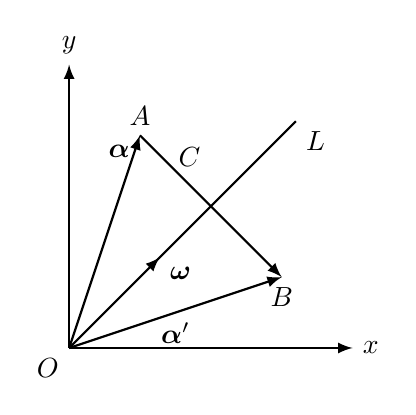
\begin{tikzpicture}[scale=1.8]
                \tikzset{>=latex, every path/.style={thick}, ->-/.style={
                    decoration={markings, mark=at position .4 with {\arrow{>}}}, postaction={decorate}
                }}
                \draw[->] (0, 0) -- (0, 2) node[above] {$y$};
                \draw[->] (0, 0) -- (2, 0) node[right] {$x$};
                \draw (0,0) coordinate (O)
                    (0.5, 1.5) coordinate (A)
                    (1.5,0.5) coordinate (B);
                \draw node[above] at (A) {$A$}
                    node[below left] at (A) {$\boldsymbol{\alpha}$}
                    node[below] at (B) {$B$};
                \draw[->] (O) -- (A);
                \draw[->] (O) -- (B)
                    node[pos=.5, below] {$\boldsymbol{\alpha}'$};
                \draw[->] (A) -- (B)
                    node[pos=.35, above=3pt] {$C$};
                \draw[->-] (O) -- (1.6, 1.6)
                    node[pos=.4, below right] {$\boldsymbol{\omega}$}
                    node[below right] {$L$};
                \draw node[below left] at (O) {$O$};
            \end{tikzpicture}
        \end{center}
\end{example}

\begin{proof}
    事实上,设直线 $L$ 的某个方向的单位向量为$\omega$,则$\vec{OC}=(\alpha,\omega)\omega$,其中$(\alpha,\omega)$为向量$\alpha$和$\omega$的内积,对于刚接触内积的读者来说,这可能并不是这么显然,但是稍加思考,我们发现这是很自然的,因为$\vec{OC}$是$\vec{OA}$在$\omega$方向上的投影,而求一个向量在另一个向量上的投影,我们高中时已经见了无数遍了,不妨设$\vec{OA}$与$\omega$的夹角为$\theta$,则$\vec{OC}=\vert\alpha \vert cos\theta\omega$,又
    \[
        \vert\alpha \vert\cos\theta=\vert\alpha \vert\dfrac{\alpha\cdot\omega}{\vert \alpha\vert\cdot\vert\omega\vert}=\dfrac{(\alpha,\omega)}{\vert\omega\vert}.
    \]
    代入单位向量模为$1$即可,不过是把我们高中的知识稍加变形罢了. 于是我们有

    \[
    \varphi(\alpha)=\alpha'=\vec{OB}=\vec{OA}+2\vec{AC}= \alpha + 2(\vec{OC}-\alpha)=-\alpha+2(\alpha,\omega)\omega.
    \]

    接下来验证 $\varphi$ 是 $\mathbf{R}^2$ 上的一个线性变换也很简单,我们留给读者自行验证.

    不过还有一个值得一提的地方\\
    如果设 $\alpha = (x,y),\omega =(\cos \theta,\sin \theta)$,则
    \begin{align*}
        \varphi(x,y)&=(-x,-y)+2(x\cos\theta+y\sin\theta)(\cos \theta,\sin \theta)\\
        &=(-x + 2x \cos^2 \theta + 2y \sin \theta \cos \theta, -y + 2x \sin \theta \cos \theta + 2y^2 \sin^2 \theta)\\
        &=(x \cos 2\theta + y \sin 2\theta, x \sin 2\theta - y \cos 2\theta).
    \end{align*}
    不难发现,这与旋转变换实质上是同一个东西,镜面变换不过是旋转了2倍的夹角罢了.
\end{proof}

\begin{summary}

\end{summary}

\begin{exercise}
    \exquote[S. 乌拉姆(Stanisław Ulam)]{一个定理有什么用并不重要,真正重要的是它有多优雅。}

    \begin{exgroup}
        \item 证明:上三角的酉矩阵必为对角矩阵.

        \item 证明:任一 $ n $ 级可逆复矩阵 $ A $ 一定可以被唯一分解成 $ A = PB $,其中 $ P $ 是 $ n $ 级酉矩阵,$ B $ 是主对角元均为正实数的 $ n $ 级上三角矩阵.
    \end{exgroup}

    \begin{exgroup}
        \item 设 $ V $ 是有限维复内积空间,$ S, T \in \mathcal{L}(V) $ 均为正规算子. 证明:若 $ ST = TS $,则
        \begin{enumerate}
            \item $ V $ 上存在一组标准正交基,使得 $ S, T $ 在此基下的矩阵都是对角矩阵.

            \item $ S $ 与 $ T $ 的复合也是正规算子.
        \end{enumerate}

        \item 设$A$为$n$阶实对称幂等矩阵,$r(A)=r$,求$|A-2E|$.
    \end{exgroup}

    \begin{exgroup}
        \item \label{item:24:镜像变换}
        \begin{enumerate}
            \item \begin{enumerate}
                      \item 设 $e$ 是欧式空间中的一个单位向量,定义线性变换
                            \[
                                \varphi(x) = x - 2\langle e, x \rangle e.
                            \]
                            证明:$\varphi$ 是正交变换且 $\det \varphi = -1$(上述 $\varphi$ 称为镜像变换);
                      \item 设 $\xi$ 是 $n$ 维欧式空间 $V$ 中的正交变换,$1$ 是 $\xi$ 的特征值且几何重数等于 $n - 1$,证明:必存在 $V$ 中的一个单位向量 $e$ 使得
                            \[
                                \xi(x) = x - 2\langle e, x \rangle e.
                            \]
                  \end{enumerate}
            \item 设 $n$ 阶矩阵 $M = E_n - 2v v^{\mathrm{T}}$,其中 $v$ 是 $n$ 维实列向量,并且满足 $v^{T}v = 1$. 这样的 $M$ 称为镜像阵. 设 $\varphi$ 是 $n$ 维欧式空间 $V$ 上的线性变换,求证:$\varphi$ 是镜像变换的充分必要条件是 $\varphi$ 在 $V$ 的某一组(任一组)标准正交基下的表示矩阵是镜像阵.
            \item 设 $u, v$ 是欧式空间 $V$ 中的两个范数相等的不同向量,求证:必存在镜像变换 $\varphi$ 使得 $\varphi(u) = v$.
            \item (Cartan–Dieudonné theorem)证明:$n$ 维欧式空间 $V$ 上的任一正交变换均可表示为不超过 $n$ 个镜像变换之积.
        \end{enumerate}
        \item 设 $n$ 为一正整数,记 $z \in \mathbb{C}^n$ 为 $z = (z_0, z_1, \ldots, z_{n - 1})$,其中 $z_i \in \mathbb{C}$. 定义 $\mathbb{C}^n$ 上的线性函数 $\omega_0, \omega_1, \ldots, \omega_{n - 1}$ 如下:
        \[
            \omega_j(z_0, z_1, \ldots, z_{n - 1}) = \dfrac{1}{\sqrt{n}}\sum_{m = 0}^{n - 1}z_m e^{-2\pi \i jm/n}.
        \]
        则离散傅里叶变换(Discrete Fourier Transform)定义为 $\mathcal{F}: \mathbb{C}^n \to \mathbb{C}^n$,其中 \[ \mathcal{F}(z) = (\omega_0(z), \omega_1(z), \ldots, \omega_{n - 1}(z)). \]
        证明:
        \begin{enumerate}
            \item $\mathcal{F}$ 是酉变换;
            \item 若定义 $z_n = z_0$,则 \[ \mathcal{F}^{-1}(z_0, z_1, \ldots, z_{n - 1}) = \mathcal{F}(z_n, z_{n - 1}, \ldots, z_1). \]
            \item $\mathcal{F}^4 = I$.
        \end{enumerate}
    \end{exgroup}
\end{exercise}

\input{./其它/未竟专题8 希尔伯特空间引论.tex}
\chapter{奇异值分解}

上一讲中我们着重介绍了内积空间上的一些特殊的算子,以及它们的约化分解. 本讲我们将尝试将所得到的结论推广到一般的线性映射上,并给出一个将一般线性映射都“对角化”的方式.

\section{奇异值分解}

我们提出要将一般的线性映射都“对角化”,但在若当标准型的时候我们已经知道,这理应是做不到的,症结在于可能没有足够的特征向量. 所以我们此处的“对角化”并不是使用线性映射本身的特征值和特征向量,而是采取与之相关的特殊的算子的特征值和特征向量. 回忆在对称矩阵部分,我们从一般的矩阵 $ A $ 构造出了 $ A^{\mathrm{T}}A $ 这样一个对称矩阵. 那么采取类似的方法,我们可以从 $ T \in \mathcal{L}(V, W) $ 构造出算子 $ T^*T $,让我们来看看它的性质.

\begin{theorem}{$ T^*T $ 的性质}{T^*T的性质}
    设 $ T \in \mathcal{L}(V, W) $,则
    \begin{enumerate}
        \item $ T^*T $ 是正算子.

        \item $ \ker T^*T = \ker T $.

        \item $ \im T^*T = \im T^* $.

        \item $ \dim \im T = \dim \im T^* = \dim \im T^*T $.
    \end{enumerate}
\end{theorem}

而正算子的特征值非负,所以我们可以做出如下的定义.

\begin{definition}{奇异值}{} \index{qiyizhi@奇异值 (singular value)}
    设 $ T \in \mathcal{L}(V, W) $,则 $ T^*T $ 的特征值的算术平方根称为 $ T $ 的奇异值,降序排列,并且每个奇异值重复 $ \dim E(\lambda, T^*T) $ 次.
\end{definition}

但这样定义出来的值如何描述 $ T $?我们先从线性映射最基本的部分开始.

\begin{theorem}{}{}
    设 $ T \in \mathcal{L}(V, W) $,则
    \begin{enumerate}
        \item $ T $ 是单射等价于 $ 0 $ 不是 $ T $ 的奇异值.

        \item $ T $ 的正奇异值的个数等于 $ \dim \im T $.

        \item $ T $ 是满射等价于 $ T $ 的正奇异值的个数等于 $ \dim W $.
    \end{enumerate}
\end{theorem}

借助 \nameref{thm:T^*T的性质}和单射满射的等价条件即可证明.

特征值对应有特征向量,奇异值也对应有奇异向量.

\begin{definition}{}{}
    设 $ T \in \mathcal{L}(V, W) $,奇异值为 $ s $,若存在 $ v \in V, w \in W $ 使得 $ Tv = sw $,$ T^*w = sv $,则称 $ v $ 为 $ T $ 关于 $ s $ 的左奇异向量,$ w $ 为 $ T $ 关于 $ s $ 的右奇异向量.
\end{definition}

$ T^*T $ 除去其特征值的性质外,更重要的在于其是一个自伴算子,所以我们可以对它应用谱定理,并由此给出我们所谓的“对角化”的方式——奇异值分解.

\begin{theorem}{奇异值分解}{} \index{qiyizhi!fenjie@奇异值分解 (singular value decomposition)}
    设 $ T \in \mathcal{L}(V, W) $ 有正奇异值 $ s_1, \ldots , s_m $. 则存在 $ V $ 的一组标准正交组 $ e_1, \ldots, \e_m $ 和 $ W $ 的标准正交组 $ f_1, \ldots, f_m $ 使得 $ \forall v \in V $ 均有$ Tv = s_1 \langle v, e_1 \rangle f_1 + \cdots + s_m \langle v, e_m \rangle f_m $.
\end{theorem}

\begin{proof}
    设 $ s_1, \ldots, s_n $ 为 $ T $ 的所有奇异值,也就有 $ n = \dim V $. 因为 $ T^*T $ 是正算子,所以对其应用谱定理,存在 $ V $ 的标准正交基 $ e_1, \ldots, e_n $ 使得 $ T^*Te_k = s_k^2e_k $,$ k = 1, \ldots, n $.

    首先对正奇异值部分进行讨论. 对 $ k = 1, \ldots, m $,令 $ f_k = \dfrac{1}{s_k}Te_k $,即对应的右奇异向量. 则对于 $j, k \in \{1, \ldots, m\}$,有

    \[
        \langle f_j, f_k \rangle = \dfrac{1}{s_j s_k} \langle Te_j, Te_k \rangle = \dfrac{1}{s_j s_k} \langle e_j, T^*Te_k \rangle = \dfrac{1}{s_j s_k} \langle e_j, s_k^2e_k \rangle = \dfrac{s_k}{s_j} \langle e_j, e_k \rangle = \delta_{jk}.
    \]

    所以 $ f_1, \ldots, f_m $ 是 $ W $ 的标准正交组. 事实上,考虑到左奇异向量和右奇异向量分别是 $ T^*T $ 和 $ TT^* $ 的特征向量,这一点是显然的.

    而对于零奇异值部分,$k \in \{m+1, \ldots, n\}$,$ T^*Te_k = 0 $,且 $ \ker T^*T = \ker T $,所以 $ Te_k = 0 $.

    从而 $ \forall v \in V $,有

    \begin{align*}
        Tv & = T(\langle v, e_1 \rangle e_1 + \cdots + \langle v, e_n \rangle e_n)       \\
           & = \langle v, e_1 \rangle Te_1 + \cdots + \langle v, e_m \rangle Te_m        \\
           & = s_1 \langle v, e_1 \rangle f_1 + \cdots + s_m \langle v, e_m \rangle f_m.
    \end{align*}

    命题得证.
\end{proof}

对于线性映射而言,使用两组不同的基是稀疏平常的事情;但对于算子而言,我们频繁地使用同一组基来表示,经常忽视了这一点. 所以,我们将所有一般线性映射“对角化”的方法建立在使用两组不同的基上,这与若当标准型的结果并不矛盾.

由此我们也可以得出 $ T $ 在这两组标准正交基下的矩阵表示,设为 $ A = (a_{ij})_{m \times n} $,则 $ a_{ij} = \begin{cases}
        s_i, & 1 \leqslant i = j \leqslant m, \\
        0,   & \text{其他情况}.
    \end{cases} $. 其形式也非常类似于对角矩阵,我们将其定义为\term{矩形对角矩阵}.

\begin{definition}{矩形对角矩阵}{} \index{juxingduijiaojuzhen@矩形对角矩阵 (rectangular diagonal matrix)}
    设 $ A = (a_{ij})_{m \times n} $,则称 $ A $ 为矩形对角矩阵,若 $ a_{ij} = 0 $ 当 $ i \neq j $ 时.
\end{definition}

通过线性映射的矩阵表示的过程,我们也可以得到矩阵形式的奇异值分解.

\begin{theorem}{}{}
    设 $ A $ 为一 $ m \times n $ 阶矩阵,则 $ A $ 的奇异值分解为 $ A = U\Sigma V^* $,其中 $ U $ 为 $ m \times m $ 阶酉矩阵,$ V $ 为 $ n \times n $ 阶酉矩阵,$ \Sigma $ 为 $ m \times n $ 阶非负实数矩形对角矩阵.
\end{theorem}

这也表明所有矩阵的作用都可以分解为原空间上的旋转、拉伸和到达空间上的旋转三部分.

\section{奇异值分解的应用}

\subsection{奇异值的几何解释}

\subsection{极分解定理}

我们继续算子与数的类比. 每个非零复数 $ z $ 都可以写成如下形式

\[ z = \left(\dfrac{z}{\lvert z \rvert}\right)\lvert z \rvert = \left(\dfrac{z}{\lvert z \rvert}\right)\sqrt{\overline{z}z} \]
其中 $ \dfrac{z}{\lvert z \rvert} $ 是一个单位复数. 那么由此我们可以类比得出一个对 $ V $ 上任意算子的漂亮的描述,因其形式类似于复数极坐标分解,所以称为\term{极分解定理}.

\begin{theorem}{极分解定理}{} \index{jifenjiedingli@极分解定理 (polar decomposition theorem)}
    设 $ T \in \mathcal{L}(V) $,则存在一个等距同构 $ S \in \mathcal{L}(V) $,使得 $ T = S\sqrt{T^*T} $.
\end{theorem}

\begin{proof}
    首先 $ \forall T \in \mathcal{L}(V) $,$ T^{*}T $ 都是正算子,所以 $ \sqrt{T^*T} $ 的定义是合理的.

    然后 $ \forall v \in V $,有
    \begin{align*}
        \lVert Tv \rVert^2 = \langle Tv, Tv \rangle & = \langle T^*Tv, v \rangle                   \\
                                                    & = \langle \sqrt{T^*T}\sqrt{T^*T}v, v \rangle \\
                                                    & = \langle \sqrt{T^*T}v, \sqrt{T^*T}v \rangle \\
                                                    & = \lVert \sqrt{T^*T}v \rVert^2.
    \end{align*}

    所以 $ \forall v \in V ,\enspace \lVert Tv \rVert = \lVert \sqrt{T^*T}v \rVert $.

    由此我们定义一个线性映射 $ S_1: \im \sqrt{T^*T} \rightarrow \im T $ 为
    \[ S_1(\sqrt{T^*T}v) = Tv. \]

    接下来要做的就是把这个 $ S_1 $ 扩张成一个等距同构 $ S \in \mathcal{L}(V) $使得 $ T = S\sqrt{T^*T} $. 不过在这之前得先验证 $ S_1 $ 是良定义的.

    设 $ v_1, v_2 \in V $ 使得 $ \sqrt{T^*T}v_1 = \sqrt{T^*T}v_2 $,则
    \begin{align*}
        \lVert Tv_1 - Tv_2 \rVert & = \lVert T(v_1 - v_2) \rVert                    \\
                                  & = \lVert \sqrt{T^*T}(v_1 - v_2)\rVert           \\
                                  & = \lVert \sqrt{T^*T}v_1 - \sqrt{T^*T}x_2 \rVert \\
                                  & = 0,
    \end{align*}

    得出 $ Tv_1 = Tv_2 $,所以 $ S_1 $ 是良定义的. 线性性结合范数便可以验证,不多赘述.

    从而 $ \forall u \in \im \sqrt{T^*T} $ 有 $ \lVert S_1u \rVert = \lVert u \rVert $.

    特别地,$ S_1 $ 是单射,由线性映射基本定理可得
    \[ \dim \enspace \im \sqrt{T^*T} = \dim \enspace \im T. \]
    而这也代表着 $ \dim(\im \sqrt{T^*T})^{\perp} = \dim(\im T)^{\perp} $. 那么就可以取 $ (\im \sqrt{T^*T})^{\perp} $ 的一组标准正交基 $ e_1, \ldots , e_m $ 和$ (\im T)^{\perp} $ 的一组标准正交基 $ f_1, \ldots, f_m $. 因为两个空间的维数相同,所以这两组标准正交基的长度相同(记为 $ m $).

    由此定义线性映射 $ S_2: (\im \sqrt{T^*T})^{\perp} \rightarrow (\im T)^{\perp} $ 为
    \[ S_2(a_1e_1 + \cdots + a_me_m) = a_1f_1 + \cdots + a_mf_m. \]
    所以 $ \forall w \in (\im \sqrt{T^*T})^{\perp} $ 均有 $ \lVert S_2w \rVert = \lVert w \rVert $.

    到这里我们想要的等距同构 $ S $ 就已经呼之欲出了. $ \forall v \in V, v = u + w $,其中 $ u \in \im \sqrt{T^*T} $,$ w \in (\im \sqrt{T^*T})^{\perp} $,将 $ S $ 定义为
    \[ Sv = S_1u + S_2w. \]

    $ \forall v \in V $ 均有
    \[ S(\sqrt{T^*T}v) = S_1(\sqrt{T^*T}v) = Tv, \]

    所以 $ T = S\sqrt{T^*T} $. 下面就是确确实实地证明 $ S $ 事实上是一个等距同构.

    $ \forall v \in V $,有
    \[ \lVert Sv \rVert^2 = \lVert S_1u + S_2w \rVert^2     = \lVert S_1u \rVert^2 + \lVert S_2w \rVert^2 = \lVert u \rVert^2 + \lVert w \rVert^2 = \lVert v \rVert^2 \]

    命题得证.
\end{proof}

极分解定理将所有一般的算子表成了一个等距同构和一个正算子的乘积,而这两种算子我们之前的章节都已经给出了完全的描述. 所以我们也得到了一般算子的第二种刻画方式.

\subsection{特征人脸算法}

奇异值分解的存在性在经典的人脸识别算法——特征人脸算法中得到了应用,使得最原始版本的特征人脸算法得以大幅加速. 首先介绍如下符号:

\begin{itemize}
    \item $m$: 人脸数量
    \item $n$: 每张人脸图像的像素数
    \item $D = \begin{pmatrix}
        x_1^\mathrm{T} \\
        \vdots \\
        x_m^\mathrm{T} \\
    \end{pmatrix}\in \mathbf{R}^{m\times n}$: 人脸数据矩阵,每一行 $x_i^\mathrm{T} \in \mathbf{R}^n$ 代表一张人脸图像
    \item $A=D - \overline{D}$: 中心化后的人脸数据矩阵,其中$\overline{D} = \begin{pmatrix}
        \overline{x}^\mathrm{T} \\
        \vdots \\
        \overline{x}^\mathrm{T} \\
    \end{pmatrix}$,$\overline{x} = \mathbf{E}(X) = \dfrac{1}{m}\sum\limits_{i=1}^m x_i$
\end{itemize}

从概率论的观点来看,具体的人脸 $x_1, \ldots, x_m$ 都是从自然人脸随机变量 $X$ 中的具体观测值,服从一个复杂的概率分布. 利用 $X$ 的协方差矩阵 (covariance matrix) 可以刻画人脸之间的相关性,即

\[ \mathrm{Cov}(X) = \dfrac{1}{m-1}\sum_{i=1}^m (x_i - \mathbf{E}(X))(x_i - \mathbf{E}(X)) = \dfrac{1}{m-1} A^{\mathrm{T}}A \]

特征人脸算法的本质在于将人脸图像从高维的像素矩阵表示 $x\in \mathbf{R}^n$ 投影到一个低维的特征空间,并寻求最小的投影损失. 主成分分析方法证明,选择协方差的特征向量作为投影基,再从特征值的绝对值从高到低选择前 $k$ 个特征向量构成低维特征空间对人脸进行表示,可以得到最小的投影损失. 这就要求我们\textbf{对协方差矩阵进行特征值分解}.

在特征人脸算法的应用场景中,人脸数量 $m$ 一般只有几百张,而每张人脸图像的像素数 $n$ 一般至少也是上万的级别. 如果直接对 $A^{\mathrm{T}}A$ 进行特征值分解,计算量是非常大的. 而利用 $A$ 的\textbf{奇异值分解的存在性},可以通过对 $AA^{\mathrm{T}}$ 进行特征值分解,从而间接得到 $A^{\mathrm{T}}A$ 的前 $k$ 个特征向量,大幅减少计算量.

具体来说,根据 $A\in \mathbf{R}^{m\times n}$ 的奇异值分解的存在性,存在正交矩阵 $U\in \mathbf{R}^{m\times m}$(左奇异矩阵)和 $V\in \mathbf{R}^{m\times m}$ (右奇异矩阵)使得

\[ A = U\Sigma V^{\mathrm{T}} \]

其中 $\Sigma = (s_{ij})_{m\times n}$, $s_{ii}=s_i$ 是奇异值,$\Sigma$ 中除了 $s_{ii}$ 之外的元素全为零. 由于

\begin{gather*}
    AA^{\mathrm{T}} = (U\Sigma V^{\mathrm{T}})(U\Sigma V^{\mathrm{T}})^{\mathrm{T}} = U \Sigma (V^{\mathrm{T}} V) \Sigma U^{\mathrm{T}} = U \Sigma^2 U^{\mathrm{T}} \\
    A^{\mathrm{T}}A = (U\Sigma V^{\mathrm{T}})^{\mathrm{T}}(U\Sigma V^{\mathrm{T}}) = V \Sigma (U^{\mathrm{T}} U) \Sigma V^{\mathrm{T}} = V \Sigma^2 V^{\mathrm{T}}
\end{gather*}

可以看出这就是用正交变换将 $A^{\mathrm{T}}A$ 和 $AA^{\mathrm{T}}$ 对角化的过程. 可以证明,奇异值分解所需要的矩阵 $U, V$ , 就分别是 $AA^{\mathrm{T}}$ 和 $A^{\mathrm{T}}A$ 的正交特征向量矩阵.

将 $U$, $V$ 用列向量形式表示:

\[ U = (u_1, \ldots, u_m), \quad V = (v_1, \ldots, v_n) \]

$u_i, v_i$ 分别为 $U, V$ 对应位置的特征向量,共享特征值 $\lambda_i$(即奇异值 $s_i$ 的平方). 根据 $u_i$ 是 的$AA^{\mathrm{T}}$ 的特征向量,有

\[ AA^{\mathrm{T}} u_i = \lambda_i u_i \]

两边左乘 $A^{\mathrm{T}}$,根据 $\lambda_i$ 对矩阵为数乘可将其提到最左边,可以得到

\[ (A^{\mathrm{T}}A)A^{\mathrm{T}} u_i = \lambda_i A^{\mathrm{T}} u_i \]

可知 $A^{\mathrm{T}} u_i$ 就是 $A^{\mathrm{T}}A$ 的特征向量,根据对应关系,就是 $v_i$ . 因此有

\[ (v_1, \ldots, v_k) = A^{\mathrm{T}}(u_1, \ldots, u_k) \]

$v_1, \ldots, v_k$ 就是我们希望将人脸投影到的低维特征空间,$k$ 是手工选择的一个控制特征空间维度的参数. 由于实践中 $k$ 一般取小于 $m$ 的值已经能达到很小的投影损失,因此仅对 $AA^{\mathrm{T}}$ 进行特征值分解是可行的.


\subsection*{算子范数}

\begin{summary}

\end{summary}

\begin{exercise}
    % \exquote[]{}

    \begin{exgroup}
        \item
    \end{exgroup}

    \begin{exgroup}
        \item
    \end{exgroup}

    \begin{exgroup}
        \item
    \end{exgroup}
\end{exercise}

\chapter{线性代数与几何}

解析几何很大程度上是线性代数发展的初衷,在研究点线面以及几何体时,将集体的几何问题抽象化为代数问题使其方便解决与计算,即是解析几何的主要思想. 本节我们将会从线性代数的角度探究解析几何的一些基本概念与方法. 此在线性代数课程的考察中也会有少部分的解析几何内容,但内容较浅,主要考察点、直线、平面等之间的关系.

\section{欧氏空间上的运算}

我们也已经基本掌握了模、内积、夹角等在内积空间中的基本概念,在此我们引入一些在先前的学习中接触较少的概念.
\begin{definition}{点积}{} \index{dianji@点积 (dot product)}
    \term{点积}是在三维欧氏空间中对两个向量的运算,用$\vec{a}\cdot\vec{b}$表示. 两向量点积得到的数值等于两向量模长的乘积与两向量夹角的余弦的乘积.
\end{definition}
特别的,三维欧氏空间中的向量点积$(a_1,a_2,a_3)\cdot(b_1,b_2,b_3)$可以表示为\[a_1b_1+a_2b_2+a_3b_3\]
由点积的计算,我们可以很方便地得到两向量夹角的余弦,即\[\cos\theta=\frac{\vec{a}\cdot\vec{b}}{|\vec{a}||\vec{b}|}\]
\begin{definition}{叉乘}{} \index{chacheng@叉乘 (cross product)}
    \term{叉乘}是在三维欧氏空间中对两个向量的运算,用$\vec{a}\times\vec{b}$表示. 两向量叉乘得到的向量垂直于两向量,方向遵循右手定则,其模长为两向量的模的乘积与两向量夹角的正弦的乘积.
\end{definition}
由定义可知,叉乘仅在三维欧氏空间中有定义,且叉乘的结果是一个向量,而不是一个数. 关于叉乘向量的计算有另一种更常用的用行列式表示的计算方法,即
\[(a_1,a_2,a_3)\times(b_1,b_2,b_3)=\begin{vmatrix}
        \vec{i} & \vec{j} & \vec{k} \\
        a_1     & a_2     & a_3     \\
        b_1     & b_2     & b_3
    \end{vmatrix}\]
其中$\vec{i},\vec{j},\vec{k}$为三维欧氏空间的自然基.

在解析几何中,叉乘的一个重要应用是求解与两向量垂直的向量.
\begin{definition}{混合积}{} \index{hunheji@混合积 (mixed product)} \index{biaoliangsancongji@标量三重积 (scalar triple product)}
    \term{混合积}(或称\term{标量三重积},不同于\term{矢量三重积})是三维欧氏空间中对三个向量的运算,用$[\vec{a},\vec{b},\vec{c}]$表示,等价于$(\vec{a}\times\vec{b})\cdot\vec{c}$.
\end{definition}
混合积的几何意义是以$\vec{a},\vec{b},\vec{c}$为邻边的平行六面体的体积,可以用行列式表示为
\[[(a_1,a_2,a_3),(b_1,b_2,b_3),(c_1,c_2,c_3)]=\begin{vmatrix}
        a_1 & a_2 & a_3 \\
        b_1 & b_2 & b_3 \\
        c_1 & c_2 & c_3
    \end{vmatrix}\]
同时读者也不难验证 $ (\vec{a}\times\vec{b})\cdot\vec{c} = \vec{a}\cdot(\vec{b}\times\vec{c}) $. 其应用之一是可以用来判断三个向量是否共面.

\section{点、直线、平面的表示}

一个点在欧氏空间中可以用一个向量来表示. 在三维欧氏空间中,我们可以用三个实数来表示一个点的坐标.

\subsection{平面的方程}

平面是欧氏空间中的一个基本几何对象,我们有多种代数方法来表示平面.

平面的一般方程是平面的一种最基本的表示方法,即$Ax+By+Cz+D=0$. 平面的一般方程十分简洁,但是我们很难由此方程得到平面的几何性质,因此我们还需要考虑其他的表示方法. 例如,一个平面由平面上一点与平面上两个不共线的向量来表示. 假设已知平面上一点$P(x_0,y_0,z_0)$和平面上两个不共线的向量$\vec{u}=(a,b,c)$和$\vec{v}=(d,e,f)$,则平面上的任意一点$Q(x,y,z)$都满足$\overrightarrow{PQ}$与$\vec{u}$和$\vec{v}$线性相关,即
\[\overrightarrow{PQ}=k_1\vec{u}+k_2\vec{v}\]
化为坐标形式即为
\[\begin{cases}
        x=x_0+k_1a+k_2d \\
        y=y_0+k_1b+k_2e \\
        z=z_0+k_1c+k_2f
    \end{cases}\]
这就是平面的参数方程,其中$k_1,k_2$是参数.

此外,平面还可以由平面上一点和平面的法向量来表示. 假设已知平面上一点$P(x_0,y_0,z_0)$和平面的法向量$\vec{n}=(A,B,C)$,则平面上的任意一点$Q(x,y,z)$都满足向量$\overrightarrow{PQ}$与$\vec{n}$垂直,即点积为0. 由此可得其方程为\[A(x-x_0)+B(y-y_0)+C(z-z_0)=0\]这种表示方法称为\term{点法式}.

我们发现这跟平面的一般方程十分相似,实际上,我们可以直接通过平面的一般方程得到平面的法向量.

在得到一张由其他方式表示的平面时,我们往往也会将其转化为一般式或点法式,以便于我们计算其与其他几何对象的关系. 例如,得到一个由平面上一点与平面上两不共线的向量表示的平面,则可以通过求两向量的叉积得到平面的法向量,从而得到平面的点法式.

\begin{example}{}{}
    若已知一个平面上有三点$A(1,2,0),\enspace B(0,1,-1),\enspace C(1,1,1)$,求该平面的一般方程.
\end{example}

\subsection{直线的方程}

直线在欧氏空间中也是一个基本对象,同样有多种代数方法可以表示直线.

首先直线可以用某两张平面的交表示. 假设有两相交平面的方程,联立可得直线方程
\[\begin{cases}
        A_1x+B_1y+C_1z+D_1=0 \\
        A_2x+B_2y+C_2z+D_2=0
    \end{cases}\]
即为直线的一般方程. 这种联立方程的表示方法最为基本,但是不够简洁,大多情况下也不够直观. 所以更多情况下我们希望在表示中可以直观体现直线的一些特征. 因此,可以用直线上的一个点和直线的方向(即方向向量)来确定一条直线.

假设已知直线上的一点$A_0(x_0,y_0,z_0)$和直线的方向向量$\vec{l}=(a,b,c)$,则直线上的任意一点$A(x,y,z)$都满足$\overrightarrow{AA_0}$与$\vec{l}$平行,用具体的方程则表示为
\[\frac{x-x_0}{a}=\frac{y-y_0}{b}=\frac{z-z_0}{c}\]
其中$a,b,c$不为零. 这种表示方法称为\term{点向式}.

如果我们对上述式子进行替换,令\[t=\frac{x-x_0}{a}=\frac{y-y_0}{b}=\frac{z-z_0}{c}\]
则可得
\[\begin{cases}
        x=x_0+at \\
        y=y_0+bt \\
        z=z_0+ct
    \end{cases}\]
这样就得到了直线的参数方程,其中$t$为参数.

当然还有以两点确定一条直线的表示方法,我们可以轻松地算出直线的方向向量,然后用点向式或参数方程来表示. 最后可以得出方程
\[\frac{x-x_1}{x_2-x_1}=\frac{y-y_1}{y_2-y_1}=\frac{z-z_1}{z_2-z_1}\]

那么如何实现从一般方程到点向式或参数方程的转换呢?最简单的方法是求解线性方程组再用两点表示或者参数表示,但是这样的方法比较麻烦,事实上我们可以利用法向量进行转换. 假设两平面的一般方程为$A_1x+B_1y+C_1z+D_1=0$与$A_2x+B_2y+C_2z+D_2=0$,则可以得到两平面的法向量分别为$\vec{n}_1=(A_1,B_1,C_1),\enspace\vec{n}_2=(A_2,B_2,C_2)$,因为该直线在两张平面内,所以直线与两个法向量都垂直,所以$\vec{n}_1\times\vec{n}_2$即为直线的方向向量. 再求出一般方程的一个解(即直线上一点)即可得到直线的点向式与参数方程.

\section{平面与直线间的位置关系}

对于三维欧氏空间中的几何对象,我们主要需要研究平行、相交与重合等关系. 我们可以通过平面与直线的方程来判断.

\subsection{线与线的位置关系}

线与线之间的位置关系判断主要依靠它们的方向向量. 如果两条直线的方向向量平行,则两条直线平行或重合,此时再判断两直线是否存在公共点,若联立方程有解,说明两直线重合,否则两条直线平行. 如果两条直线的方向向量不平行,则还需要判断两条直线是否共面,若共面则说明两条直线相交,否则两条直线异面. 此时以两直线方程联立方程组,若有解则说明存在交点,否则说明两条直线异面.

\begin{example}{}{}
    已知直线$L_1=\begin{cases}
            x+y+z-1=0 \\
            x-2y+2=0
        \end{cases},\enspace L_2=\begin{cases}
            x=2t  \\
            y=t+a \\
            z=bt+1
        \end{cases}$,试确定$a,b$的值使得$L_1,L_2$是:
    \begin{enumerate}
        \item 平行直线;

        \item 异面直线.
    \end{enumerate}
\end{example}

\subsection{线与面的位置关系}

线与面的位置关系首先需要判断线的方向向量与平面的法向量的关系. 如果方向向量与法向量平行,则说明线与面垂直. 如果两者垂直,则说明该直线与平面平行或者在平面内,只需再判断直线上的点是否在平面内即可.

此外还有一些对于平面不同表示形式的方法. 例如,假设已知直线的方向向量与平面上两个不平行的向量,则可以对这三个向量做混合积,如果混合积为零,则说明三个向量共面,即直线与平面平行或者在平面内.

\subsection{面与面的位置关系}

面与面的位置关系主要依靠两个平面的法向量来判断. 如果两个平面的法向量平行,则说明两个平面平行或重合,再判断两平面是否存在公共点. 若两法向量垂直,则两平面也垂直.

\subsection{平面与点的位置关系}
一个空间中的平面 $\Gamma$ 可以以一个方程表示:
\[
A x + B y + C z + D = 0
\]
它的一个法向量是 $\vec{n} = (A, B, C)$,因此我们说一个向量 $\vec{a}$ 在平面 $\Gamma$ 中当且仅当
\[
\langle \vec{n}, \vec{a} \rangle = -D
\]
一个简单的观察是,$D$ 表征了平面和原点之间的距离. 实际上,平面和原点之间的距离就是
\[
d_{O\text{-}\Gamma} = \frac{\abs{D}}{\sqrt{A^2 + B^2 + C^2}}
\]
这并不难估计,只需注意到
\[
\langle \vec{n}, \frac{-D}{A^2 + B^2 + C^2}\vec{n} \rangle = -D
\]
即可. 另一种计算方式也可由截距入手,读者可自行计算直角四面体的体积,这留作一个习题. 有了这个式子之后,我们就能考虑任意一点到平面的距离. 这种考虑的第一个步骤是考虑怎么将某个点``移作''原点,实际上,设这个点的向量表示为 $\vec{b}$,我们就有一个新的以内积的形式作的表示:
\[
\left\langle \vec{n}, \vec{a} + \vec{b} \right\rangle = -D
\]
利用线性性将其写开,并移项,得到新的平面的常数项:
\[
D' = \langle \vec{n}, \vec{b} \rangle + D
\]
将此式代入到已有的方程中,就能得到:
\[
d_{\vec{b}\text{-}\Gamma} = \frac{\abs{\langle \vec{n}, \vec{b} \rangle + D}}{\sqrt{A^2 + B^2 + C^2}}
\]
或者,如果你宁愿为了得到一个更为优雅的方程而多加一些标记,把 $\vec{b}$ 记作 $(x_0, y_0, z_0)$,则可以得到结果:
\[
d_{\vec{b}\text{-}\Gamma} = \frac{\abs{A x_0 + B y_0 + C z_0 + D}}{\sqrt{A^2 + B^2 + C^2}}
\]
另一种同样利用内积的推导方式是利用 Cauchy-Schwartz 不等式,同样见诸习题.

另一个式子是球方程. 就球而言,我们需要考虑的事情其实很少. 一个圆心为 $\vec{a}$,半径为 $r$ 的球 $C$ 中的点 $\vec{x}$ 满足方程:
\[
\langle \vec{x} - \vec{a}, \vec{x} - \vec{a} \rangle = r^2
\]
如果你乐意的话,也可以将其展开:
\[
\langle \vec{x}, \vec{x} \rangle - 2 \langle \vec{x}, \vec{a} \rangle + \langle \vec{a}, \vec{a} \rangle - r^2 = 0
\]
它是一个二次的形式. 对它而言,我们更关注的是它的另外一个性质:其切点的向量表示就是切面的一个法向量,在后面的讨论中,这将是至关重要的一点. 因为相切关系的平移不变性,我们给出以下结果:

\begin{theorem}{}{}
球 $\langle \vec{x}, \vec{x} \rangle = r^2$ 与平面 $\langle \vec{n}, \vec{x} \rangle = -D$ 在点 $\vec{t}$ 处相交,且总共有且仅有一个交点(即相切)当且仅当:
\begin{enumerate}
    \item $\langle \vec{t}, \vec{t} \rangle = r^2, \quad \langle \vec{n}, \vec{t} \rangle = -D$,即 $\vec{t}$ 既在圆上,也在平面上;
    \item 存在 $\lambda \in \R$ 使得 $\vec{t} = \lambda \vec{n}$ 成立,即 $\vec{t}$ 和 $\vec{n}$ 共线.
\end{enumerate}
\end{theorem}

这个命题的证明与命题本身一样显而易见,只要利用二次方程的求根公式即可,与圆和直线相切的推导别无二致,请读者自行完成证明.

\section{射影空间与仿射变换}

在不考虑内积的情况下,在向量空间中的几何性质当中,实际上只有共线性和共线点之间的比例是特殊的. 在此,我们定义

\begin{definition}{}{}
    称一个保持共线性和定比分点性质的映射为仿射变换(affine transformation).
\end{definition}

一个重要的结论如下:
\begin{theorem}{}{}
    $\R^n \to \R^m$ 的仿射变换全体就是所有形如
    \[
    F(u) = A u + v
    \]
    的映射全体
\end{theorem}

这个结论告诉我们,仿射变换就是线性变换的一种推广. 它实际上就是线性变换和平移操作的复合. 这个结论的证明并不复杂:

\begin{proof}
    零点的像平移、基的像线性变换(利用共线性和定比分点性质推导出线性变换的定义).
\end{proof}

% 例子:平移、旋转、拉伸、斜截

但是,这样的记号多少有点不够精致. 我们知道的线性变换有了非常丰富的性质,所以我们也希望能够把仿射变换做成某种线性映射. 考虑一个更加形式性的解法:
\[
A u + v = \begin{pmatrix}
    A & v \\
    0 & 1
\end{pmatrix} \begin{pmatrix}
    u \\ 1
\end{pmatrix}
\]
作为分块矩阵,它们自然地能够满足仿射变换的需求,但是它将一个 $\R^n \to \R^m$ 的仿射变换表示为了一个 $\R^{n + 1} \to \R^{m + 1}$ 的线性变换. 但是,这样的表示依然是不够充分的. 这是因为我们``要求''向量为一个末尾为 $1$ 的向量,而矩阵的最后一行也被确定为一个末尾为 $1$ 的行向量. 基于此限制的线性变换是``过度受限''的. 因此,我们希望更多地以几何的方式解读这些限制,而不是以代数的方式将其强加到空间之上.

回顾对平面方程的讨论. 我们业已提及,一个平面的表达式就是
\[
\langle \vec{n}, \vec{a} \rangle = -D
\]
注意到,这里的法向量 $\vec{n}$ 是没有正规化的. 也就是说,实际上平面方程由两种东西决定:一是 $\vec{n}$ 的坐标,一是 $-D$ 的取值,而且实际上平面方程就相当于
\[
\langle (\vec{n}, D), (\vec{a}, 1) \rangle = 0
\]
而且左边的向量似乎可以在相差一个倍数的意义下表示同一个平面. 因此,我们定义:
\begin{definition}{}{}
    称空间 $\R^{n + 1}$ 关于如下等价关系构成的等价类为 $n$ 维实射影空间:
    \[
    x \sim y \iff \exists k \in \R, x = k y
    \]
    将其构成的集合全体记作 $\mathbf{PR}^n$.
\end{definition}

现在,我们完成了从代数到几何最关键的一步:通过一个等价关系,原来的线性空间变成了一个看上去相当奇怪的结构. 但是,它把捉了几何上重要的``比值''关系. 接下来的部分当中,我们就需要讨论实射影空间所具备的结构特征.

注意到,在射影空间之间,存在一个事实上很平凡的嵌入关系:
\begin{lemma}{}{}
    $\mathbf{PR}^{n - 1}$ 能够被自然地嵌入到 $\mathbf{PR}^n$ 当中,此嵌入映射如下:
    \[
    [x] \mapsto [(x, 0)]
    \]
\end{lemma}

证明只需要验证这个映射的良定性即可. 不难发现,这个映射实际上是一个单射. 而且在去掉所有形如 $[(x, 0)]$ 的等价类之后,剩下的所有等价类就是所有形如 $[(x, 1)]$ 的等价类. 也就是说:
\begin{theorem}{}{}
    实射影空间 $\mathbf{PR}^n$ 无非是 $\R^{n - 1}$ 和 $\mathbf{PR^{n - 1}}$ 的无交并.
\end{theorem}

通过一个更简单的想法可以更好地理解这样的结构:射影直线 $\mathbf{PR}^1$ 就是一个 $\R$ 并上一个``无穷远点'',射影平面 $\mathbf{PR}^2$ 就是一个 $\R^2$ 并上一个无穷远处的射影直线. 推而广之,一个射影空间 $\mathbf{PR}^n$ 就是一个 $R^{n - 1}$ 并上一个无穷远处的子射影空间 $\mathbf{PR}^{n - 1}$.

那么,对于我们的目的而言,这有什么用呢?实际上,可以表明:

\begin{theorem}{}{}
    一个 $\R^n \to \R^m$ 的仿射变换可以被写成一个 $\mathbf{PR}^n \to \mathbf{PR}^m$ 的线性映射的商,且子空间 $\mathbf{PR}^{m - 1}$ 的原像包含于子空间 $\mathbf{PR}^n$ 当中.
\end{theorem}

也就是说,我们现在的操作如下图所示:
\[
\begin{tikzcd}
    \R^n \dar \rar & \R^{n + 1} \dar \rar & \mathbf{PR}^n \dar \rar & \R^n \dar \\
    \R^m \rar & \R^{m + 1} \rar & \mathbf{PR}^m \rar & \R^m
\end{tikzcd}
\]

\section{曲面上的标架}

考虑曲面 $S$ 的参数化,将其写成下面的形式:
\[
\begin{cases}
x = x(u, v) \\
y = y(u, v) \\
z = z(u, v)
\end{cases}
\]

考虑导数
\[
\vec{t}_u = (x_{u}, y_{u}, z_{u}), \quad \vec{t}_v = (x_{v}, y_{v}, z_{v})
\]

对微积分有所了解的读者应该不难看出,这两个向量是曲面在某个点的切向量. 考虑一个ˋˋ好的''参数化,即在任意点这样的两个切向量线性无关. 这样的参数网对于满足一些可微性条件的曲面来说总是存在的,在此不做证明. 我们定义:
\begin{definition}
    称切向量 $\vec{t}_u |_{\vec{t}_0}, \vec{t}_v |_{\vec{t}_0}$ 所张成的向量空间为曲面 $S$ 在 $\vec{t_0}$ 点的切平面,记作 $T_{\vec{t}_0} S$.
\end{definition}
切平面的单位法向量称为这个点处曲面的法向量,记作 $\vec{n}$. 不难发现,在曲面上的任意点上,$(\vec{t}_u, \vec{t}_v, \vec{n})$ 张成三维空间,这被称为曲面上在这个点处的自然标架.

在自然标架下,我们不难考虑曲面上某一片小区域的面积,通过一点点微积分的操作,我们可以得出:
\[
\mathrm{d} s^2 = |\vec{t}_u|^2 \mathrm{d} u^2 + 2 \vec{t}_u \cdot \vec{t}_v \mathrm{d} u \mathrm{d} v + |\vec{t}_v|^2 \mathrm{d} v^2
\]
我们定义:
\begin{align*}
    E &= |\vec{t}_u|^2 \\
    F &= \vec{t}_u \cdot \vec{t}_v \\
    G &= |\vec{t}_v|^2
\end{align*}
不难发现,$E > 0, G > 0, E G - F^2 > 0$,我们可以将其写成矩阵的形式:
\[
\begin{pmatrix}
    E & F \\
    F & G
\end{pmatrix}
\]
这种形式通常被称作曲面的第一基本形式. 不难发现,它给定了曲面上的长度和面积.

考虑坐标变换
\[
\begin{cases}
    \tilde{u} = \tilde{u}(u, v) \\
    \tilde{v} = \tilde{v}(u, v)
\end{cases}
\]
我们探讨在此变换下(如果这个变换之后的结果也是``好的''),第一基本形式会发生什么样的变化. 记变换之后的第一基本形式为:
\[
\begin{pmatrix}
    \tilde{E} & \tilde{F} \\
    \tilde{F} & \tilde{G}
\end{pmatrix}
\]
可以证明:
\begin{theorem}{}{}
    变换前后的第一标准形式与原来的第一标准形式有如下关系:
    \[
    \begin{pmatrix}
        \tilde{E} & \tilde{F} \\
        \tilde{F} & \tilde{G}
    \end{pmatrix}
     =
    J^\mathrm{T} \begin{pmatrix}
        E & F \\
        F & G
    \end{pmatrix} J
    \]
    其中 $J$ 为 Jacobi 矩阵,形式如下:
    \[
    \begin{pmatrix}
        \dfrac{\partial u}{\partial \tilde{u}} & \dfrac{\partial u}{\partial \tilde{v}} \\ \\
        \dfrac{\partial v}{\partial \tilde{u}} &
        \dfrac{\partial v}{\partial \tilde{v}}
    \end{pmatrix}
    \]
\end{theorem}

证明基于 Jacobi 矩阵的含义来完成.

\begin{proof}
    将 $\mathrm{d} s^2$ 按照一阶的形式展开.
\end{proof}

我们会意识到,这个``乘上一个可逆矩阵及其转置''的形式是非常重要的. 在后文中,我们会称之为矩阵的相合标准型. 由此,读者亦可窥见此定义的重要性.

\section{二次曲面及其分类}

下面我们考虑一族简单的曲面,令
\[
S: a x^2 + b y^2 + c z^2 + 2 d y z + 2 e x z + 2 f x y + g x + h y + i z = 1
\]
其中关于 $x, y, z$ 都是二次的,称作二次曲面. 下面我们想问的是,如何对二次曲面完成分类. 注意到,上面的方程也可以被写成:
\[
S: \begin{pmatrix}
    x & y & z
\end{pmatrix}
\begin{pmatrix}
    a & f & e \\
    f & b & d \\
    e & d & c
\end{pmatrix}
\begin{pmatrix}
    x \\ y \\ z
\end{pmatrix} + \begin{pmatrix}
    g & h & i
\end{pmatrix} \begin{pmatrix}
    x \\ y \\ z
\end{pmatrix} = 1
\]

一般地,前面的形式 $v^\mathrm{T} A v$ 被称为``二次型'',在后面我们会花费一整讲的时间来讨论有关于它的理论. 但是在此之前,我们先思考如何对二次曲面进行分类.

上面的方程可以简记作:
\[
v^\mathrm{T} A v + b^\mathrm{T} v = 1
\]

首先,我们考虑对 $A$ 进行谱分解. 由于 $A$ 是实对称矩阵,所以它可以被写成 $Q^\mathrm{T} \Lambda Q$ 的形式,其中 $\Lambda$ 为对角矩阵,$Q$ 为正交矩阵. 我们知道,正交矩阵对应的是一个等距同构. 所以,我们将其先写成:
\[
v^\mathrm{T} Q^\mathrm{T} \Lambda Q v + b^\mathrm{T} Q^\mathrm{T} Q v = 1
\]
于是,将 $Q v$ 置为 $\tilde v$,则能得到方程:
\[
\tilde v^\mathrm{T} \Lambda \tilde v^\mathrm{T} + \tilde b^\mathrm{T} \tilde v' = 1
\]
其中 $\tilde b = Q^\mathrm{T} b$.

此时我们对应到二次曲面,实际上是通过一次等距同构消掉了 $d, e, f$ 三个系数. 我们得到的方程就变成了
\[
S: ax^2 + by^2 + cz^2 + g x + h y + i z = 1
\]
通过我们熟知的配方法,我们可以把左式变成
\[
S: a(x - \frac{g}{2a})^2 - \frac{g^2}{4a} + b(y - \frac{h}{2b})^2 - \frac{h^2}{4b} + c(z - \frac{i}{2c})^2 - \frac{i^2}{4c} = 1
\]
也就是说,通过一个平移变换,就能将原式变成
\[
a x^2 + b y^2 + c z^2 = d
\]
的形式.

总结上述讨论,我们可以得到以下定理:

\begin{theorem}{}{}
    任意二次曲面经过等距变换都可以得到满足如下曲面方程的曲面:
    \[
    a x^2 + b y^2 + c z^2 = d
    \]
\end{theorem}

注意到一点,这里的 $a, b, c$ 是原先的矩阵
\[
\begin{pmatrix}
    a & f & e \\
    f & b & d \\
    e & d & c
\end{pmatrix}
\]
的特征值. 也就是说,对于一个二次曲面的方程,这个矩阵的特征值几乎决定了它的几何结构,这在后面的分类讨论给出每种曲面的形式之后将能够更清晰地展现. 一个有意思的观察是,对于二次曲线,我们也能得出类似的结果,这留作一个习题,请读者自行完成分类. 而在后面的学习中,我们会发现,对于更高维度空间中的二次曲面,这依然是一个重要的分类依据.

\begin{summary}

\end{summary}

\begin{exercise}
    \exquote[笛卡尔]{我决心放弃那个仅仅是抽象的几何. 这就是说,不再去考虑那些仅仅是用来练思想的问题. 我这样做,是为了研究另一种几何,即目的在于解释自然现象的几何.}

    \begin{exgroup}
        \item 用等体积法计算原点到平面的距离. 考虑 $A, B, C$ 均非零的平面 $A x + B y + C z + D = 0$,计算:
        \begin{enumerate}
            \item 平面在 $x, y, z$ 轴上的截距以及三个截点与平面构成的直角四面体的体积.
            \item 三个截点围成的三角形的面积.(提示:运用 Helen 公式或者秦九韶公式).
            \item 给出平面到原点的距离公式,并与文中的公式比对.
        \end{enumerate}

        \item 用 Cauchy-Schwartz 不等式证明点到平面的距离公式.
    \end{exgroup}

    \begin{exgroup}
        \item 考虑平面曲线 \[A x^2 + B y^2 + C x y + D x + E y + F = 0\] 的分类.(提示:类比上面对空间二次曲面的分类,找出变换方式和判据)
    \end{exgroup}

    \begin{exgroup}
        \item
    \end{exgroup}
\end{exercise}

\chapter{二次型}

\section{二次型的定义}

在几何部分中,我们讨论了二次曲线和二次曲面的分类. 对于平面二次曲线
\[ax^2 + by^2 + cxy + dx + ey + f = 0,\]
常见的处理手段是通过旋转变换消去交叉项$xy$,然后平移变换消去一次项,最终得到标准形式. 类似的多项式和变换形式在数学与物理中也有很多应用,为了方便我们考虑二次齐次多项式,也就引入了二次型的概念.

\begin{definition}{二次型}{} \index{ercixing@二次型 (quadratic form)}
    $n$个元$x_1,x_2,\ldots,x_n$的二次齐次多项式
    \begin{align*}
        f(x_1,x_2,\ldots,x_n) & = \sum_{i=1}^{n}a_{ii}x_i^2+\sum\limits_{1\leqslant i<j\leqslant n}2a_{ij}x_ix_j    \\
                              & = a_{11}x_1^2+a_{22}x_2^2+\cdots+a_{nn}x_n^2                                        \\
                              & \quad +2a_{12}x_1x_2+\cdots+2a_{1n}x_1x_n+2a_{23}x_2x_3+\cdots+2a_{n-1,n}x_{n-1}x_n
    \end{align*}
    称为域$\mathbf{F}$上的$n$元二次型(简称\term{二次型}).
\end{definition}
先考虑实域上的情况. 若令$a_{ij}=a_{ji}\enspace(1\leqslant i<j\leqslant n)$,则二次型可表示为
\[f(x_1,x_2,\ldots,x_n)=\sum_{i=1}^{n}\sum_{j=1}^{n}a_{ij}x_ix_j=X^\mathrm{T}AX\]
其中$X=(x_1,x_2,\ldots,x_n)^\mathrm{T}\in\mathbf{R}^n$,$A=(a_{ij})_{n\times n}$为实对称矩阵,并称对称矩阵$A$为二次型$f(x_1,x_2,\ldots,x_n)$的相伴矩阵.

\begin{example}{}{}
    已知二次型
    \[f(X)=(x_1,x_2,x_3,x_4)\begin{pmatrix}
            1 & 2 & 3 & -4 \\ 3 & 2 & 1 & 4 \\ -4 & 3 & -7 & 2 \\ 0 & -6 & 8 & 4
        \end{pmatrix}\begin{pmatrix}
            x_1 \\ x_2 \\ x_3 \\ x_4
        \end{pmatrix}\]
    写出二次型$f(X)$的相伴矩阵.
\end{example}

实际上一个形如$f(x_1,x_2,\ldots,x_n)=\displaystyle\sum_{i=1}^{n}\sum_{j=1}^{n}a_{ij}x_ix_j$的函数可以对应的矩阵是很多的,但不唯一的矩阵表示会给我们带来很多不便. 而选取对称矩阵作为二次型的相伴矩阵,不仅是因为简化了计算,还是因为二次型和对称矩阵之间存在一一对应的关系.

\begin{example}{}{}
    回答以下问题:
    \begin{enumerate}
        \item 已知$A$是一个$n$阶矩阵,则$A$为反对称矩阵的充要条件是对任意$n$元列向量$X$都有$X^\mathrm{T}AX=0$;

        \item 若二次型$f(x_1,x_2,\ldots,x_n)=X^\mathrm{T}AX$对任意$n$元列向量$X$都有$f(x_1,x_2,\ldots,x_n)=0$,证明:$A=O$;

        \item 设二次型$f(x_1,x_2,\ldots,x_n)=X^\mathrm{T}AX,\enspace g(x_1,x_2,\ldots,x_n)=X^\mathrm{T}BX$.\\
              证明:若$f(x_1,x_2,\ldots,x_n)=g(x_1,x_2,\ldots,x_n)$,则$A=B$.
    \end{enumerate}
\end{example}

\section{矩阵相合的定义与性质}

二次型的基本问题是寻找一个线性变换将其变换为只包含平方项的所谓“标准形”,这反映在矩阵上便是对角化. 而我们将二次曲线标准化的操作抽象出来,便会发现这是我们熟悉的坐标变换. 考虑原坐标为$X$,新坐标为$Y$,原二次型为$f(X) = X^\mathrm{T}AX$. 因为变换是线性的,并且坐标长度不变,因此我们有$X=PY$,其中$P$是可逆矩阵. 而用$Y$代换$X$,便可以得到$g(Y) = Y^\mathrm{T}(P^\mathrm{T}AP)Y$,虽然未必能立刻得到标准形,但这一变换是二次型的一个基本操作,我们称之为相合变换.

\begin{definition}{}{}
    我们称$n$阶矩阵$A$相合于$B$(记作$A\simeq B$),如果存在可逆矩阵$C$使得$B=C^\mathrm{T}AC$.
\end{definition}
矩阵相合(合同)有如下基本性质:
\begin{enumerate}
    \item 合同是等价关系;合同不同于相似,是与域有关的;合同要求$C$必须可逆,因此是一种特殊的相抵;

    \item $A\simeq B$一般不能得到$A^m\simeq B^m$(但是$A,B$为实对称矩阵时可以),但如果可逆,我们有$A^{-1}\simeq B^{-1}$,同时如果$A_1\simeq A_2,B_1\simeq B_2$,则有$\begin{pmatrix}
                  A_1 & O \\ O & B_1
              \end{pmatrix}\simeq\begin{pmatrix}
                  A_2 & O \\ O & B_2
              \end{pmatrix}$;

    \item $A\simeq B$表明$A$可以每次做相同的初等行列变换得到$B$,反之亦然.
\end{enumerate}

% \begin{example}{}{}
%     设$A\simeq B$,$C\simeq D$,且它们都是$n$阶实对称矩阵,问:$A+C\simeq B+D$ 是否成立.
% \end{example}

% \begin{example}{}{}
%     判断:矩阵相似是否一定合同?矩阵合同是否一定相似?对于实对称矩阵上述论断又是否正确呢?正确请说明理由,不正确请举出反例.
% \end{example}

\section{二次型标准形的定义与求解}

所以用矩阵的语言表示的话,求解二次型的标准形就是寻找可逆矩阵 $C$ 使得 $C^\mathrm{T}AC$ 为对角矩阵. 最基础的想法就是如同相抵标准型那样,通过初等变换将矩阵变换为对角矩阵.

\begin{lemma}{}{初等变换与合同变换引理1}
    对称矩阵 $A$ 的下列变换都是相合变换:
    \begin{enumerate}
        \item 对换 $A$ 的第 $i$ 行与第 $j$ 行,再对换第 $i$ 列与第 $j$ 列;

        \item 将非零数 $k$ 乘以 $A$ 的第 $i$ 行,再将 $k$ 乘以 $A$ 的第 $i$ 列;

        \item 将 $A$ 的第 $i$ 行乘以 $k$ 加到第 $j$ 行,再将 $A$ 的第 $i$ 列乘以 $k$ 加到第 $j$ 列.
    \end{enumerate}
\end{lemma}

接下来的问题是,如何进行合适的初等变换来将一个对称矩阵对角化.

\begin{lemma}{}{初等变换与合同变换引理2}
    设 $A$ 是域 $\mathbf{F}$ 上的非零对称矩阵,则必定存在可逆矩阵 $C$ 使得 $C^\mathrm{T}AC$ 的第 $(1, 1)$ 个元素不为 $0$.
\end{lemma}

\begin{proof}
    \begin{enumerate}
        \item 若 $a_{11} = 0$ 而 $a_{ii} \neq 0$,则将 $A$ 的第 $1$ 行与第 $i$ 行对换,再将第 $1$ 列与第 $i$ 列对换,即可使得 $a_{11} \neq 0$.
        \item 若 $a_{ii} = 0, \forall i$,那么设 $a_{ij} \neq 0(i \neq j)$,将 $A$ 的第 $j$ 行加到第 $i$ 行,再将第 $j$ 列加到第 $i$ 列. 因为 $A$ 是对称矩阵,所以 $a_{ij} = a_{ji} \neq 0$,第 $(i, i)$ 元素在变换后变为 $2 a_{ij} \neq 0$,便可根据第一种情况处理.
    \end{enumerate}
    而根据\autoref{lem:初等变换与合同变换引理1},这些变换都是相合变换,结论得证.
\end{proof}

由此,便可以得到以下结论.

\begin{theorem}{}{}
    设 $A$ 是域 $\mathbf{F}$ 上的 $n$ 阶对称矩阵,则必存在 $\mathbf{F}$ 上的 $n$ 阶可逆矩阵 $C$,使得 $C^\mathrm{T}AC$ 为对角矩阵.
\end{theorem}

\begin{proof}
    由\autoref{lem:初等变换与合同变换引理2},不妨设 $A = (a_{ij})$ 中 $a_{11} \neq 0$,若 $a_{i1} \neq 0$,则可将第 $1$ 行乘以 $-a_{11}^{-1}a_{i1}$ 加到第 $i$ 行上,再将第 $1$ 列乘以 $-a_{11}^{-1}a_{i1}$ 加到第 $i$ 列上,因为 $a_{i1} = a_{1i}$,所以新得到的矩阵的第 $(i, 1)$ 元素和第 $(1, i)$ 元素均等于 $0$,并且和 $A$ 相合. 重复这一过程,便可以将 $A$ 的第 $1$ 列和第 $1$ 行的非对角元素全部变为 $0$,所以 $A$ 相合与以下形式的矩阵:
    \[
        \begin{pmatrix}
            a_{11} & 0 & 0 & \cdots & 0 \\
            0 & b_{22} & b_{23} & \cdots & b_{2n} \\
            0 & b_{32} & b_{33} & \cdots & b_{3n} \\
            \vdots & \vdots & \vdots & \ddots & \vdots \\
            0 & b_{n2} & b_{n3} & \cdots & b_{nn}
        \end{pmatrix}.
    \]
    右下角是一个 $n - 1$ 阶对称矩阵,记为 $A_1$,根据归纳假设,存在 $n - 1$ 阶可逆矩阵 $D$ 使得 $D^\mathrm{T}A_1D$ 为对角矩阵,所以
    \[
        \begin{pmatrix}
            1 & O \\
            O & D^\mathrm{T}
        \end{pmatrix}
        \begin{pmatrix}
            a_{11} & O \\
            O & A_1
        \end{pmatrix}
        \begin{pmatrix}
            1 & O \\
            O & D
        \end{pmatrix} = \begin{pmatrix}
            a_{11} & O \\
            O & D^\mathrm{T}A_1D
        \end{pmatrix}
    \]

    是一个对角阵,并且

    \[
        \begin{pmatrix}
            1 & O \\
            O & D
        \end{pmatrix}^\mathrm{T} = \begin{pmatrix}
            1 & O \\
            O & D^\mathrm{T}
        \end{pmatrix}
    \]

    所以 $A$ 相合于对角阵.
\end{proof}

注意到整个证明过程暗含了如何利用初等矩阵得到相合标准形的操作,但如果想要得到坐标变换矩阵 $C$ 还需要一点额外的操作.

\begin{example}{}{相合标准形例1}
    利用初等变换法将二次型 $f(x_1,x_2,x_3)=2x_1x_2-2x_1x_3+2x_2x_3$ 化为标准形,并且求出坐标变换矩阵$C$.
\end{example}

\begin{solution}
    类似于利用初等变换求矩阵的逆,我们将相伴矩阵和单位矩阵拼接为 $\begin{pmatrix}
        A \\ E
    \end{pmatrix}$,对 $A$ 进行初等行列变换,使其变为对角矩阵,同时对 $E$ 进行对应的列变换,最终得到的 $\begin{pmatrix}
        \Lambda \\ C
    \end{pmatrix}$ 就是我们要求的结果.

    \begin{align*}
        \left(\begin{array}{c}
            A \\ \hdashline E
        \end{array}\right) ={} & \left(\begin{array}{ccc}
            0 & 1 & -1 \\
            1 & 0 & 1  \\
            -1 & 1 & 0 \\
            \hdashline
            1 & 0 & 0 \\
            0 & 1 & 0 \\
            0 & 0 & 1
        \end{array}\right)
        \xrightarrow[r_1+r_2]{c_1+c_2} \left(\begin{array}{ccc}
            2 & 1 & 0 \\
            1 & 0 & 1  \\
            0 & 1 & 0 \\
            \hdashline
            1 & 0 & 0 \\
            1 & 1 & 0 \\
            0 & 0 & 1
        \end{array}\right) & \\
        \xrightarrow[r_2-\dfrac{1}{2}r_1]{c_2-\dfrac{1}{2}c_1} & \left(\begin{array}{ccc}
            2 & 0 & 0 \\
            0 & -\dfrac{1}{2} & 1  \\
            0 & 1 & 0 \\
            \hdashline
            1 & -\dfrac{1}{2} & 0 \\
            1 & \dfrac{1}{2} & 0 \\
            0 & 0 & 1
        \end{array}\right)
        \xrightarrow[r_3+2r_2]{c_3+2c_2} \left(\begin{array}{ccc}
            2 & 0 & 0 \\
            0 & -\dfrac{1}{2} & 0  \\
            0 & 0 & 2 \\
            \hdashline
            1 & -\dfrac{1}{2} & -1 \\
            1 & \dfrac{1}{2} & 1 \\
            0 & 0 & 1
        \end{array}\right) & \\
    \end{align*}
\end{solution}

初等变换法虽然泛用性比较广,但是操作起来比较繁琐,通常情况下使用配方法更加方便. 配方法的思想非常简单,就是利用配方消除混合乘积项,将二次型表示成几个平方和的形式,最后通过坐标变换$X=CY$化标准形,其中$C$是可逆矩阵.

\begin{example}{}{相合标准形例2}
    用配方法把三元二次型
    \[f(x_1,x_2,x_3)=2x_1^2+3x_2^2+x_3^2+4x_1x_2-4x_1x_3-8x_2x_3\]
    化为标准形,并求所用的坐标变换$X=CY$即变换矩阵$C$.
\end{example}

配方法的合理性是可逆的坐标变换所保证的,只要配方成功的消除了所有交叉项,便可以得到标准形. 但配方法在处理一些情况的时候需要一些技巧,比如\autoref{ex:相合标准形例1},需要先通过坐标变换构造出平方项,再通过配方法消除交叉项.

不过需要注意的是,以上两种方法得到的对角矩阵不一定是相伴矩阵的相似对角化,相似对角化要求是 $P^{-1}AP$ 为对角矩阵,而相合对角化是 $P^\mathrm{T}AP$ 为对角矩阵,二者一致的话需要满足 $P^{-1} = P^\mathrm{T}$,也就是说 $P$ 是正交矩阵. 不过这一点并不是难以做到的,因为 $A$ 是实对称矩阵,根据\nameref{thm:实谱定理},$A$ 的标准化后的特征向量组成的矩阵便是正交矩阵$P$,所以我们也可以通过正交变换求解二次型的相合标准形.

\begin{example}{}{}
    用正交变换法将二次型 $f(x_1,x_2) = 2x_1^2 + 5x_2^2 + 4x_1x_2$ 化为标准形,并给出变换矩阵 $P$.
\end{example}

\section{相合规范形 \quad 惯性定理}

从前面求解相合标准形的例子可以发现,使用配方法、初等变换法得到的相合标准形,会因为配方方式或者初等变换顺序不同而各不相同,所以相合标准形并不是唯一的. 但相抵标准形是唯一的,相似标准形不考虑特征值排列组合因素也是唯一的,因此我们也希望统一相合标准形.

不难发现,任一对角矩阵一定相合于$\diag(1,\ldots,1,-1,\ldots,-1,0,\ldots,0)$,我们称这一相合标准形为相合规范形,其中$+1$的个数称为矩阵的正惯性指数,$-1$的个数称为矩阵的负惯性指数. 并且由于变换矩阵可逆,根据相抵标准形的结论,我们有原矩阵$A$的秩$r(A)$等于这一对角矩阵的秩,于是也等于正负惯性指数之和. 显然,$A$可逆时,其相合规范形主对角元没有0.

但我们没有说明一个矩阵的相合规范形是否唯一,实际上这就是下面惯性定理的结果:
\begin{theorem}{惯性定理}{}
    实对称矩阵的相合规范形唯一.
\end{theorem}
这一定理有很多等价表述,例如实对称矩阵正、负惯性指数唯一,或者实对称矩阵相合标准形中对角线上正、负、零的个数唯一. 或者实对称矩阵特征值中正、负、零的个数唯一等.

\begin{proof}
    采取证明等价表述:实对称矩阵正、负惯性指数唯一.

    设 $f(X) = X^\mathrm{T}AX$ 为一实二次型,通过可逆坐标变换$X = BY$ 和 $X = CZ$ 得到了相合规范形
    \begin{align*}
        f ={} & y_1^2 + \cdots + y_p^2 - y_{p+1}^2 - \cdots - y_r^2 \\
          ={} & z_1^2 + \cdots + z_k^2 - z_{q+1}^2 - \cdots - z_r^2.
    \end{align*}
    其中 $r$ 为 $A$ 的秩,我们希望证明此时一定有$p = k$,使用反证法.

    假设 $p > k$,由 $Z = C^{-1}X = C^{-1}BY$,定义 $D = C^{-1}B$,则 $Z = DY$,写作线性方程组的形式为

    \[
        \begin{cases}
            z_1 & = d_{11}y_1 + \cdots + d_{1n}y_n, \\
            z_2 & = d_{21}y_1 + \cdots + d_{2n}y_n, \\
            & \vdotswithin{=} \\
            z_k & = d_{k1}y_1 + \cdots + d_{kn}y_n, \\
            & \vdotswithin{=} \\
            z_{n} & = d_{n1}y_1 + \cdots + d_{nn}y_n.
        \end{cases}
    \]

    矛盾的构造点在于 $f$ 的取值,比较明显的构造便是一种表达下为正,而另一种表达下为负. 所以令 $z_1 = z_2 = \cdots = z_k = 0$,以及 $y_{p + 1} = y_{p + 2} = \cdots = y_n = 0$. 结合上面列出的方程组,我们可以得到新的方程组.

    \[
        \begin{cases}
            d_{11}y_1 + d_{12}y_2 + \cdots + d_{1n}y_n & = 0, \\
            d_{21}y_1 + d_{22}y_2 + \cdots + d_{2n}y_n & = 0, \\
            & \vdotswithin{=} \\
            d_{k1}y_1 + d_{k2}y_2 + \cdots + d_{kn}y_n & = 0. \\
            y_{p + 1} = 0, \\
            y_{p + 2} = 0, \\
            \cdots \\
            y_n = 0.
        \end{cases}
    \]

    这一方程组有 $n$ 个变量,但只有 $k + (n - p) = n - (p - k) < n$ 个方程,所以必定有非零解,而 $y_{p + 1} = y_{p + 2} = \cdots = y_n = 0$,说明 $y_1, y_2, \ldots, y_p$ 不全为 $0$. 代入 $f$ 的表达式,可以得到

    \[
        f = y_1^2 + y_2^2 + \cdots + y_p^2 > 0.
    \]

    将 $Y$ 代入 $Z$ 关于 $Y$ 的方程中,再将得到的 $Z$ 代入 $f$ 的表达式,因为 $z_1 = z_2 = \cdots = z_k = 0$,所以

    \[
        f = -z_{k + 1}^2 - z_{k + 2}^2 - \cdots - z_n^2 \leqslant 0.
    \]

    这两者显然矛盾,所以 $p > k$ 不成立,必然有 $p \leqslant k$,同理可证 $k \leqslant p$,所以 $p = k$,也就有实对称矩阵的相合规范形唯一.

\end{proof}

\begin{example}{}{}
    确定二次型$f(x_1,x_2,\ldots,x_{10})=x_1x_2+x_3x_4+x_5x_6+x_7x_8+x_9x_{10}$的秩以及正、负惯性指数.
\end{example}

惯性定理的``惯性''二字与物理中的惯性有关,实际上透露着某种不变性. 根据惯性定理,我们有如下结论:
\begin{enumerate}
    \item 我们可以按相合关系对全体$n$阶实对称矩阵分类,因为实对称矩阵相合意味着规范形唯一,我们可以按照$+1$、$-1$、0个数的不同划分为$\vphantom{\cfrac{n+1}{2}}\dfrac{(n+1)(n+2)}{2}$个等价类;

    \item 实域上两个实对称矩阵相合的充要条件是它们有相同的正负惯性指数,两个对角矩阵相合的充要条件是对角线上正、负、零个数相同.
\end{enumerate}

而对于复二次型,若其已经化为标准形
\[
    f(X) = d_1x_1^2 + d_2x_2^2 + \cdots + d_rx_r^2,
\]
其中 $d_i \neq 0$,$r$ 为该矩阵的秩. 设 $d_j = r_j(\cos \theta_j + \i \sin \theta_j)$,$0 \leqslant \theta_j < 2 \pi$ 那么根据棣莫弗公式(De Moivre's Formula),有
\[
    (\pm \sqrt{r_j}(\cos \dfrac{\theta_j}{2} + \i \sin \dfrac{\theta_j}{2}))^2 = d_j.
\]
记 $\sqrt{r_j}(\cos \dfrac{\theta_j}{2} + \i \sin \dfrac{\theta_j}{2})$ 为 $\sqrt{d_j}$,那么做如下的坐标变换$X=CY$,其中
\[C = \diag(\dfrac{1}{\sqrt{d_1}}, \ldots, \dfrac{1}{\sqrt{d_r}}, 1, \ldots, 1)\]
便可以将复二次型化为标准形
\[
    f(Y) = y_1^2 + \cdots + y_r^2.
\]
所以复二次型的标准形是唯一的,只与其秩有关.

\section{正定二次型和正定矩阵}

二次型的保号性也是其被广泛研究并运用的原因之一.

\begin{definition}{}{}
    设 $f(X) = X^\mathrm{T}AX$ 是 $n$ 元实二次型,$A$ 是相伴矩阵.
    \begin{enumerate}
        \item 若对任意非零 $n$ 元实列向量 $X$,都有 $f(X) > 0$,则称 $f(X)$ 是正定二次型,$A$ 是正定矩阵;
        \item 若对任意非零 $n$ 元实列向量 $X$,都有 $f(X) \geqslant 0$,则称 $f(X)$ 是半正定二次型,$A$ 是半正定矩阵;
        \item 若对任意非零 $n$ 元实列向量 $X$,都有 $f(X) < 0$,则称 $f(X)$ 是负定二次型,$A$ 是负定矩阵;
        \item 若对任意非零 $n$ 元实列向量 $X$,都有 $f(X) \leqslant 0$,则称 $f(X)$ 是半负定二次型,$A$ 是半负定矩阵;
        \item 若存在 $n$ 元实列向量 $X_1, X_2$,使得 $f(X_1) > 0$ 且 $f(X_2) < 0$,则称 $f(X)$ 是不定二次型.
    \end{enumerate}
\end{definition}

其中我们重点研究正定和半正定二次型,因为负定和半负定二次型可以通过符号变换得到.

很自然的一个问题是如何判断一个二次型是正定或半正定的,我们也期望使用二次型内禀的性质来判断矩阵的性质. 显然
\[f(X) = x_1^2 + x_2^2 + \cdots + x_n^2\]
是一个正定二次型,它也是相合规范形的一种. 而对于
\[g(X) = x_1^2 + x_2^2 + \cdots + x_{n - 1}^2 + 0 \cdot x_n^2,\]
我们便可以构造出$X_n=(0, 0, \ldots, 0, 1)$使得$g(X)=0$,但去除掉$X_n$生成的子空间和零向量后,剩下的$X$都满足$g(X) > 0$,这是一个半正定二次型. 所以我们可以感觉到正定二次型的条件应当较为严苛,半正定二次型的条件略有放松,但都应该和惯性指数有着密切的联系,这也符合于我们的直觉.

\begin{theorem}{}{}
    设$f(X)$是$n$元实二次型,$A$是$f(X)$的相伴矩阵,$r$为$A$的秩,$r_+$为$A$的正惯性指数. 则
    \begin{enumerate}
        \item $f(X)$是正定二次型当且仅当$r_+=n$;
        \item $f(X)$是半正定二次型当且仅当$r_+=r$.
    \end{enumerate}
\end{theorem}

由此而得到的一个显然的推论如下:

\begin{corollary}{}{}
    $n$阶实对称矩阵$A$是正定矩阵当且仅当其合同于单位阵$E_n$,是半正定矩阵当且仅当其合同于对角阵$\begin{pmatrix}
        E_r & O \\ O & O
    \end{pmatrix}$.
\end{corollary}

所以考虑正定矩阵$A$,其经过合同变换得到单位阵$E_n$,即$C^\mathrm{T}AC = E_n$,两侧取行列式有$\det(C^\mathrm{T})\det(A)\det(C)=\det(C)^2\det(A)=\det(E_n)=1$,所以$\det(A)>0$,即正定矩阵的行列式大于$0$. 而考虑对正定矩阵做限制,即只取前$r$行$r$列,得到的$r$阶子矩阵也是正定矩阵,回忆\hyperref[def:子式、主子式、顺序主子式]{顺序主子式的定义},这启示我们可以通过顺序主子式的符号来判断矩阵的正定性.

\begin{theorem}{}{}
    $n$阶实对称矩阵$A$是正定阵的充分必要条件是$A$的所有顺序主子式的行列式都大于$0$.
\end{theorem}

\begin{example}{}{}
    求$t$的取值范围,使得下面的二次型是正定的:
    \[f(x_1,x_2,x_3,x_4) = x_1^2+4x_2^2+4x_3^2+3x_4^2+2tx_1x_2-2x_1x_3+4x_1x_2.\]
\end{example}

而通过一些简单的行列对换,我们可以得到这一定理的推论:
\begin{corollary}{}{}
    若 $A$ 是正定矩阵,则:
    \begin{enumerate}
        \item $A$的任一$k$阶主子阵都是正定阵;
        \item $A$的所有主子式均为正,特别地,$A$的主对角元素全大于零.
    \end{enumerate}
\end{corollary}

再考虑对正定二次型进行正交变换,得到$f(X) = \lambda_1 x_1^2 + \lambda_2 x_2^2 + \cdots + \lambda_n x_n^2$,其中$\lambda_i$均为$A$的特征值,显然根据上面的推论我们也可以得到如下定理:

\begin{theorem}{}{}
    $n$元实二次型$f(X)$的特征值都是正数当且仅当$f(X)$是正定二次型.
\end{theorem}

不过也可以根据正定矩阵的分解得到以上的结论,对于正定矩阵,我们有如下的引理:

\begin{lemma}{}{}
    设$A$是$n$阶实对称矩阵,那么$A$是正定矩阵的充要条件是存在$n$阶可逆矩阵$C$使得$A=C^\mathrm{T}C$.
\end{lemma}

设$\lambda$为$A$的任一特征值,$X$为对应的特征向量,则有$AX = \lambda X$,代入引理得到$C^\mathrm{T}CX = \lambda X$,两侧同时左乘$X^\mathrm{T}$,得到
\begin{gather*}
    X^\mathrm{T}C^\mathrm{T}CX = \lambda X^\mathrm{T}X, \\
    (CX)^\mathrm{T}(CX) = \lambda X^\mathrm{T}X,
\end{gather*}

取欧几里得内积,得到
\[||CX||^2 = \lambda ||X||^2,\]
因为$C$可逆且$X \neq 0$,所以$\lambda > 0$,即$A$的特征值均为正数.

在先前我们介绍过$LU$分解,对于正定矩阵,我们有更加高效的分解方法,即 Choelsky 分解.

\begin{theorem}{}{Choelsky 分解}
    对于正定矩阵$A$,存在唯一的下三角矩阵$L$使得$A=LL^\mathrm{T}$,并且$L$的对角元素均为正数.
\end{theorem}

半正定矩阵关于以上的结论也是类似的,但相应地有条件的减弱,以及部分等价条件不再成立.
\begin{theorem}{}{}
    若$A$为$n$阶实对称矩阵,则
    \begin{enumerate}
        \item 若$A$为半正定矩阵,则$A$的顺序主子式非负;
        \item $A$为半正定矩阵等价于$A$的各阶主子式非负;
        \item 若$A$为半正定矩阵,则存在矩阵$C$使得$A=C^{\mathrm{T}}C$(注意$C$未必可逆);
        \item $A$为半正定矩阵等价于$A$的所有特征值非负.
        \item 若$A$为半正定矩阵,则存在对角线上元素非负的下三角矩阵$L$使得$A=LL^{\mathrm{T}}$.
    \end{enumerate}
\end{theorem}

而到如今,我们回望实内积空间时,会发现所谓的 Gram 矩阵其实就是一个半正定矩阵,内积也可以写作一个二次型的形式. 使用任意一个半正定矩阵都可以定义一个内积,而内积空间的基本性质也可以通过半正定矩阵的性质来推导.但对于复内积空间来说,这就依赖于 Hermite 型和 Hermite 矩阵的性质了,不再过多展开.

\section{标准形的应用}

我们已经讨论了三种标准形,即相抵标准形,相似标准形和相合标准形,实际上它们之间的关系我们已经讨论,即相似一定相抵,相合一定相抵,但相似和相合互相没有包含关系. 本节我们考虑一些基于矩阵分解的问题,利用之前所学的相抵标准形、相似标准形、相合标准形的分解解决一些问题. 本节内容可以选择性掌握.

首先看一个关于幂等矩阵的例题,需要用到相抵标准形、相似标准形的分解:
\begin{example}{}{}
    解答以下两个问题:
    \begin{enumerate}
        \item 证明:任意一个方阵都可以分解成一个可逆矩阵和一个幂等矩阵的乘积;

        \item 已知$A$是一个秩为$r$的$n$级非零矩阵,证明:$A$为幂等矩阵的充要条件是存在列满秩的$n\times r$矩阵$B$和行满秩的$r\times n$矩阵$C$使得$A=BC$且$CB=E_r$.
    \end{enumerate}
\end{example}
下面是一个利用相合标准形进行分解的例子:
\begin{example}{}{}
    (与正交有关)证明:每个秩为$r$的$n\enspace(r<n)$阶实对称矩阵均可表示为$n-r$个秩为$n-1$的实对称矩阵的乘积.
\end{example}

\begin{summary}

\end{summary}

\begin{exercise}
    % \exquote[]{}

    \begin{exgroup}
        \item 设$A=\begin{pmatrix}
            1 & 2 & 0 \\ 2 & 1 & 0 \\ 0 & 0 & 3
        \end{pmatrix},\enspace B=\begin{pmatrix}
            -2 & 0 & 0 \\ 0 & 2 & 1 \\ 0 & 1 & 2
        \end{pmatrix}$,判断$A$与$B$是否相合.
    \end{exgroup}

    \begin{exgroup}
        \item 设$n$元二次型$f(x_1,x_2,\ldots,x_n)=l_1^2+\cdots+l_p^2-l_{p+1}^2-\cdots-l_{p+q}^2$,其中$l_i\enspace (i=1,2,\ldots,p+q)$是关于$x_1,x_2,\ldots,x_n$的一次齐次式. 证明:$f(x_1,x_2,\ldots,x_n)$的正惯性指数$\leqslant p$,负惯性指数$\leqslant q$;

        \item 已知$A$为$m$阶实对称矩阵,$C$为$m\times n$实矩阵,证明:$C^\mathrm{T}AC$的正负惯性指数分别小于等于$A$的正负惯性指数.
    \end{exgroup}

    \begin{exgroup}
        \item
    \end{exgroup}
\end{exercise}

\chapter{多重线性映射与张量的计算}

在定义了线性性之后,我们不难联想到微积分中一元函数到多元函数的推广过程. 因此,我们自然地想要将线性映射推广到多重线性映射. 这时,我们顺理成章地也就完成了对向量和矩阵的推广,也就是所谓的张量. 张量的运算在几何的背景下具备明确的意义,在本讲中,我们会简要介绍张量的计算法则. 因为张量在物理学中的普遍使用,数学家、科普作家 Lillian R. Lieber 将张量誉为 the fact of universe,可见其重要性.

\section{多重线性映射}

多重线性映射的定义是轻松的. 它无非就是把一元的映射变成多元的映射,让我们直接写出 $n$ 元情形下的定义:

\begin{definition}{}{}
    设 $V_1, V_2, \ldots, V_n, W$ 均为线性空间,称 $f: V_1 \times V_2 \times \cdots \times V_n \to W$ 为\term{多重线性映射},如果它对于任意一个分量都是线性的,即
    \[ f(v_1, \ldots, \lambda v_i + \mu v_i', \ldots, v_n) = \lambda f(v_1, \ldots, v_i, \ldots, v_n) + \mu f(v_1, \ldots, v_i', \ldots, v_n) \]

    即保加法和数乘操作. 我们将这样的多重线性映射全体记为 $\mathcal{L}(V_1, V_2, \cdots, V_n; W)$. 如果 $W = \mathbf{F}$,则称 $f \in \mathcal{L}(V_1, V_2, \cdots, V_n; \mathbf{F})$ 为\term{多重线性函数}.
\end{definition}

注意,我们在记号中的最后一项用的是分号而不是逗号,其目的就是区分目标线性空间和源线性空间. 这里首先要注意到的一点是,$\mathcal{L}(V_1 \times V_2 \times \cdots \times V_n, W)$ 和 $\mathcal{L}(V_1, V_2, \cdots, V_n; W)$ 是完全不同的. 为了理解这点,我们需要注意到 $V_1 \times V_2$ 中的数乘操作是对 $(v_1,v_2) \in V_1 \times V_2$ 中的每个分量都加以数乘,而多重线性映射的数乘是可以单独作用在任意一个分量上的,请看下面的一个例子:

\begin{example}
    考虑 $V_1 = V_2 = W = \R$. 考虑映射:
    \[
    f(a, b) = ab
    \]
    则它是一个多重线性映射,因为我们有 $\forall \lambda, \mu, a_1, a_2 \in \R$
    \[
    f(\lambda a_1 + \mu a_2, b) = (\lambda a_1 + \mu a_2) b = \lambda f(a_1, b) + \mu f(a_2, b)
    \]
    对于第二个分量也是同理的. 但是如果将其理解成 $V_1 \times V_2 \to W$ 的映射,则它不是一个线性映射. 考虑数乘操作即可:
    \[
    f(\lambda (a, b)) = f(\lambda a, \lambda b) = \lambda^2 ab \neq \lambda f(a, b)
    \]
    另一方面,考虑映射
    \[
    f(a, b) = a + b
    \]
    则它是一个 $\R^2 \to \R$ 的线性映射,因为对于任意 $(a_1, b_1), (a_2, b_2) \in \R^2, \lambda, \mu \in \R$,都有
    \[
    f(\lambda (a_1, b_1) + \mu (a_2, b_2)) = f(\lambda a_1 + \mu a_2, \lambda b_1 + \mu b_2) = \lambda f(a_1, b_1) + \mu f(a_2, b_2)
    \]
    但是它不是一个多重线性映射,考虑第一个分量的数乘操作:
    \[
    f(\lambda a, b) = \lambda a + b \neq \lambda f(a, b)
    \]
    因此,多重线性映射不一定是积空间上的线性映射,乘积空间上的线性映射也不一定是多重线性映射.
\end{example}

第二个问题是,我们怎么表达这样的多重线性映射?我们知道,线性映射可以用矩阵来表达,那么,多重线性映射应该怎么表达呢?我们首先考虑二元的情形. 考虑 $V_1, V_2, W$ 都是线性空间,为了接下来讨论的方便,不失一般性地,我们所有的线性空间都直接视为 $\mathbf{F}^n$ 这样的向量空间,其中 $n$ 为向量空间的维数,之后的矩阵表示需要的基在不特殊说明的情况下均取自然基. 若 $f \in \mathcal{L}(V_1, V_2; W)$,则我们很容易想到,将 $f$ 拆成两个线性函数,设 $V_1$ 有一组基 $\{e_1,\ldots,e_n\}$,记
\[
f_i (v_2) = f(e_i, v_2)
\]
则它就是一个 $V_2 \to W$ 的线性映射. 设它所对应的矩阵为 $M_i$,考虑 $V_1$ 中的向量 $v_1 = \lambda_1 e_1 + \lambda_2 e_2 + \cdots \lambda_n e_n$,其中 $n = \dim V_1$,则
\[
f(v_1, v_2) = f(\lambda_1 e_1 + \lambda_2 e_2 + \dots + \lambda_n e_n, v_2) = \lambda_1 f_1 (v_2) + \lambda_2 f_2 (v_2) + \cdots + \lambda_n f_n (v_2)
\]
将线性映射翻译成矩阵,我们就有:
\[
f(v_1, v_2) = \lambda_1 M_1 v_2 + \lambda_2 M_2 v_2 + \cdots + \lambda_n M_n v_2 = (\lambda_1 M_1 + \lambda_2 M_2 + \cdots + \lambda_n M_n) v_2
\]
形式地,我们将其记作(回忆 $v_1 = (\lambda_1,\lambda_2,\ldots,\lambda_n)$)
\[
    f(v_1, v_2) = v_1^\mathrm{T} \begin{pmatrix}
        M_1 \\ M_2 \\ \vdots \\ M_n
    \end{pmatrix}
    v_2
\]
其中的
\[\begin{pmatrix}
        M_1 \\ M_2 \\ \vdots \\ M_n
    \end{pmatrix}\]
就是多重线性映射 $f$ 在自然基下的矩阵表示. 这个记号看起来很符合直觉:使用矩阵乘法的通常规则,我们将 $v_1$ 的每个分量 $\lambda_i$ 分别和对应的 $M_i$ 相乘然后求和,再乘以后面的 $v_2$. 但要注意的是,这不同于分块矩阵乘法,如果是分块矩阵乘法我们还要求 $\lambda_i$ 和 $M_i$ 是可以做矩阵乘法的,但显然这里并不能,因此这只是形式上的记号.

事实上,这种记号就是我们在朴素的情形下对张量的理解:一种广义矩阵,以矩阵为元素的矩阵;更广泛地说,以张量为元素的向量:我们将向量称为 $1$ 阶张量,以向量为元素的向量称为 $2$ 阶张量,就是矩阵,而以 $n$ 阶张量为元素的向量就称为 $n + 1$ 阶张量——直观地说,$3$ 阶张量就是一个“立方体”中排有的数字,而 $n$ 阶张量则是 $n$ 维的方体. 在上面的例子中,我们给出的就是一个 $3$ 阶张量,因为它涉及三个线性空间之间的映射. 如果只涉及两个线性空间,那就是我们之前介绍的线性映射,那它的表示就是 $2$ 阶张量(即矩阵).

有的读者可能会疑惑张量中元素的排列是按行还是按列的,目前我们不会区分这两者,在后文引入反变和共变的概念后再作区分.

\section{张量积}

在研究了多重线性映射的表示之后,我们要探讨的问题就是,多重线性映射构成的线性空间 $\mathcal{L}(V_1, V_2, \cdots, V_n; W)$ 的结构,即我们如何构造这样一个线性空间. 可以预计的是,它应该能够被视作是一个 $\mathcal{L}(V_1, V_2, \cdots, V_n; \R)$ 和 $W$ 组合而成的东西. 为了理解为何会如此,我们先从一个常见的情形开始:

\begin{lemma}{}{多重线性函数}
    \[
    \mathcal{L}(V, W^*; \R) \cong \mathcal{L}(V, W)
    \]
\end{lemma}

实际上,这个命题的证明无非就是把我们在最开始所做的关于多重线性映射的表示的讨论重述一遍.

\begin{proof}
    设 $V$ 有一组基 $\{e_1, e_2, \dots, e_n\}$,$f \in \mathcal{L}(V, W^*; \R)$. 记
    \[
    f_i (\rho) = f(e_i, \rho), \forall \rho \in W^*
    \]
    则 $f_i: W^* \to \R$ 是 $W^{**}$ 中的元素,基于$W^{**} \cong W$ 的同构映射 $\varphi$,我们可以得到 $W$ 中的元素 $\varphi(f_i)$. 而通过将每个 $e_i$ 映射到 $\varphi(f_i)$ 可以确定一个 $V \to W$ 的线性映射 $\psi$(基于\autoref{thm:线性映射构造}). 然后我们就可以基于此给出一个线性同构:
    \begin{center}
        \begin{tabular}{rrcl}
            $\Phi\enspace\colon$      & $\mathcal{L}(V, W^*; \R)$ & $\to$     & $\mathcal{L}(V, W)$ \\
                                   & $f$                      & $\mapsto$ & $\psi$
        \end{tabular}
    \end{center}

    基于这个构造,不难验证它是一个线性同构:
    \begin{enumerate}
        \item 线性性:
        \item 同构:
    \end{enumerate}
\end{proof}

基于上面的证明,我们很容易看出,一个多重线性函数的集合可以与一个线性映射的集合互相转化. 下面我们由此出发定义张量积:

\begin{definition}{}{}
    定义 $V_1 \otimes V_2 = \mathcal{L}(V_1^*, V_2^*; \R) \cong \mathcal{L}(V_1^*, V_2)$,称为向量空间 $V_1$ 和 $V_2$ 的张量积.
\end{definition}

根据同构关系显然有 $\dim V_1 \otimes V_2 = \dim V_1 \dim V_2$. 不难看出为什么我们要用对偶来定义这个结构. 直观地说,这其实就是原来的对偶空间的推广,因为在一个线性空间的情形下,我们就有 $\mathcal{L}(V_1^*, \R) = V_1$.

按照递推的方式,我们可以定义出更多个线性空间的张量积:
\begin{lemma}{}{}
    $(V_1 \otimes V_2) \otimes V_3 = \mathcal{L}(\mathcal{L}(V_1^*, V_2^*; \R), V_3^*; \R) \cong \mathcal{L}(V_1^*, V_2^*, V_3^*; \R) \cong \mathcal{L}(V_1^*, V_2^*; V_3).$
\end{lemma}

这个引理的证明可以仿照\autoref{lem:多重线性函数}完成,较为繁杂,此处略去. 这一引理表明了 $\otimes$ 具备结合律,因为 $\mathcal{L}(V_1^*, V_2^*, V_3^*; \R)$ 中的 $V_1^*, V_2^*, V_3^*$ 具有同等地位. 除此之外,利用归纳法我们可以得到以下推论:
\begin{corollary}{}{}
    $\dim V_1 \otimes V_2 \otimes \cdots \otimes V_n = \dim V_1 \dim V_2 \cdots \dim V_n.$
\end{corollary}

下面我们给出 $V_1 \otimes V_2$ 中的元素的表示,但是,更方便的看法其实是考虑 $V_1^* \otimes V_2^*$ 中元素的表示. 我们知道,它就是一个 $\mathcal{L}(V_1, V_2; \R)$ 中的元素,所以,考虑 $f \in V_1^*, g \in V_2^*$,记

\[
(f \otimes g) (v_1, v_2) = f(v_1) g(v_2)
\]

则 $f \otimes g \in \mathcal{L}(V_1, V_2; \R)$,不难验证它是一个双线性映射. 进一步地,$\otimes: V_1^* \times V_2^* \to \mathcal{L}(V_1, V_2; \R)$ 这个映射是一个满但不单的双线性映射:
\begin{lemma}{}{}
    $\otimes: V_1^* \times V_2^* \to \mathcal{L}(V_1, V_2; \R)$ 是一个满但不单的双线性映射.
\end{lemma}
\begin{proof}
    双线性映射 $f$ 由 $f(\alpha_i,\beta_j)$ 唯一确定.
\end{proof}

既然 $\otimes$ 不是单射,我们自然想要去计算:

\begin{lemma}{}{}
    \[
    \ker \otimes = \{(f, g) \mid (f, g) \sim (0, 0)\}
    \]
    其中 $\sim$ 为以下等价关系:
    \[
    (f_1, g_1) \sim (f_2, g_2) \iff \forall v_1, v_2, f_1(v_1) g_1(v_2) = f_2(v_1) g_2(v_2)
    \]
\end{lemma}

这个引理几乎就是 $\ker \otimes$ 定义的同义反复,而事实上,我们能写出这个引理的另一个版本:

\begin{lemma}{}{}
    $\ker \otimes = \mathop{\mathrm{span}}\{(f,0), (0, g)\}$
\end{lemma}
\begin{proof}

\end{proof}

因此,我们有了张量积的另一个定义,我们以定理的形式陈述:

\begin{theorem}{}{}
    张量积 $V_1 \otimes V_2 \cong V_1 \times V_2 / \ker \otimes$,其中 $\ker \otimes$ 如上所述.
\end{theorem}
\begin{proof}

\end{proof}

\begin{theorem}{}{张量积的基}
    张量积的一组基
\end{theorem}
\begin{proof}
    很显然,$i_k$ 不全相同的两个张量是线性无关的
\end{proof}

最后的最后,我们给出一个泛性质的描述方式. 这实际上几乎就是从商空间的泛性质继承过来的,不过多了一点多重线性代数的成分:

\begin{theorem}{}{}
    考虑 $V_1 \times V_2$ 到 $V_1 \otimes V_2$ 的典范投影 $\pi$,按照商空间的写法它应该是明显的. 那么,对于任意向量空间 $U$ 和 $V_1 \times V_2 \to U$ 的双线性映射 $\varphi$,存在唯一线性映射 $\tilde \varphi$ 使下图交换:
    \begin{center}
        \begin{tikzcd}
            V_1 \times V_2 \rar["\pi"] \arrow[rd, swap, "\varphi"] & V_1 \otimes V_2 \dar["\exists ! \tilde \varphi"] \\
             & U \\
        \end{tikzcd}
    \end{center}
\end{theorem}

细心的读者可能会发现,这里有一个记号似乎被滥用了. 我们通常所说的 $V_1 \times V_2 \to U$ 的映射都是指线性映射,而这里却用之来指代双线性映射. 对范畴论有些许了解的读者会意识到,这不是在 $\mathsf{FVect}$,即有限维线性空间构成的范畴的意义下所说的泛性质,因为其中混杂了线性映射和双线性映射. 但这其实不是问题,只需要对范畴的对象进行一些重新定义——当然,这不是我们在这里需要去深入研究的主题. 至于这个定理的证明,参照商映射的泛性质的证明,这并不困难,故留作练习.

\section{张量的坐标变换}

在以下的记号当中,我们都会用上标表示对偶空间中的指标,下标表示原空间的指标. 从此以后会采纳 Einstein 求和约定,也就是说,记:

\[
a^i x_i := \sum_{i = 1}^n a^i x_i
\]

其中 $i$ 称为哑指标,要求它在其他地方没有出现过,且同时出现在上标和下标当中. 其中的范围 $n$ 则由读者自己在语境中给出. 例如上面的表达式中,$i$ 同时出现在求和对象 $a^i x_i$ 的上下标中,而且 $i$ 没有在其他地方出现过,因此可以简写为 $a^i x_i$.

这样的表示好处在于,在以后大规模进行张量的讨论时,我们会用到大量此种求和,而上下指标的方式往往是比较方便且符合直觉的. 当然这需要适应,比如下面的例子这样更复杂的和式:

\[
a^{ij} x_i y_j = \sum_{i = 1}^n \sum_{j = 1}^m a^{ij} x_i y_j
\]

此处 $i,j$ 同时出现在了求和对象 $a^{ij} x_i y_j$ 的上下标中,因此这一求和就可以简写为 $a^{ij} x_i y_j$. 为了让读者适应一下这样的记号,考虑向量 $b$ 的分量 $b_i$ 和矩阵 $M$ 的元素 $M_{ij}$,记 $Mb = v$,其中分量为 $v_i$,则按照矩阵乘法的定义:

\[
v_i = \sum_{j = 1}^m M_{ij} b_j
\]

这样的记号难以写成 Einstein 求和,这是因为没有指标出现在上标,所以我们拨弄一下矩阵中元素的指标,写成:

\[
v_i = \sum_{j = 1}^m M^j_i b_j =: M^j_i b_j
\]

这样就简化了不少记号. 其中行号在下,列号在上,我们通常都采纳此种记法. 然后考虑矩阵乘法,考虑矩阵 $A$ 和矩阵 $B$ 以及其中的元素 $A_i^j$ 和 $B_k^l$,令 $AB = C$:

\[
C_m^n = \sum\limits_{j=1}^p A_m^j B_j^n =: A_m^j B_j^n
\]

这样,我们的记号就非常自然了. 看起来哑指标 $j$ 就像是被消掉了一样($j$ 只出现在了求和展开式中,但未出现在最后的结果 $C_m^n$ 中),非常合理. 另一个常用的例子在未来会介绍的二次型当中,考虑向量 $x, y$ 和矩阵 $A$,记号如上所述,则

\[
x^\mathrm{T} A y = \sum\limits_{i=1}^p \sum\limits_{j=1}^q x^i A_i^j y_j =: x^i A_i^j y_j
\]

这里为啥 $x$ 的分量 $i$ 写在上面呢?因为 $x$ 发生了转置,它变成了一个行向量,所以其中的元素下标就变成了列号,是上标. 实际上的话,我们更常用的写法是保持坐标为下标而矩阵全为上标,也就是说,写成:

\[
x^\mathrm{T} A y = x_i A^{ij} y_j
\]

这样按照求和约定也是合理的,在后面我们会解释为什么会出现这样的结构.

在研究矩阵的过程中,我们说过,矩阵在坐标变换之后会发生某种变化,这就是所谓的换基操作,它带来的就是相似矩阵的定义. 张量同样也不可避免地要面对基的变换的问题,而且更加复杂,这值得我们花一整节来理解并适应.

我们称 $V_1 \otimes V_2 \otimes \cdots \otimes V_n, V_i = V, \forall i = 1, 2, ..., n$ 这一张量积中的元素为张量. 事实上根据我们在第一节中的讨论,那里的张量是多重线性映射的表示,实际上和多重线性映射本身是一一对应的,因此这两个张量的定义是基本一致的.

设 $V$ 的一组基为 $\{\tilde{e}_{i}\}$,原先的基为 $\{e_i\}$. 存在矩阵 $M$ 使得其中的元素为 $M_i^j$,满足:
\[
\tilde e_{i} = M_i^j e_j
\]
注意,这里 $j$ 是被求和的哑指标. 出于习惯,让我们写出张量积空间的一组基
\[
e_{i_1 i_2 \cdots i_n} = e_{i_1} \otimes e_{i_2} \otimes \cdots \otimes e_{i_n}
\]
对于新的一组基 $\tilde{e}_{i}$,也能给出新的一组张量积空间的基,形如:
\[
\tilde{e}_{i_1 i_2 \cdots i_n} = \tilde{e}_{i_1} \otimes \tilde{e}_{i_2} \otimes \cdots \otimes \tilde{e}_{i_n}
\]
展开 $\tilde e_{i_t}$ 项,能够得到:
\[
\tilde{e}_{i_1 i_2 \cdots i_n} = M_{i_1}^{j_1} e_{j_1} \otimes M_{i_2}^{j_2} e_{j_2} \otimes \cdots \otimes M_{i_n}^{j_n} e_{j_n}
\]
其中 $j_k$ 是哑指标. $M_{i_k}^{j_k}$ 是一个纯粹的实数,我们可以将其提到最前面,并重新整理一下求和:
\[
\tilde{e}_{i_1 i_2 \cdots i_n} = \sum_{j_1, j_2, \ldots, j_n} \left( \prod_k M_{i_k}^{j_k} \right) e_{j_1} \otimes e_{j_2} \cdots \otimes e_{j_n} = \left( \prod_k M_{i_k}^{j_k} \right) e_{j_1 j_2 \cdots j_n}
\]
注意其中 $k$ 取遍 $1, 2, \cdots, n$,最后一式中 $j_l$ 均为哑指标.
注意到,一个张量积空间中的元素是
\[
T = \tilde T^{i_1 i_2 \cdots i_n} \tilde e_{i_1 i_2 \cdots i_n} = \tilde T^{i_1 i_2 \cdots i_n} \tilde e_{i_1} \otimes \tilde e_{i_2} \otimes \cdots \otimes \tilde e_{i_n}
\]
其中 $i_k$ 均为哑指标. $\tilde T^{i_1 i_2 \cdots i_n}$ 是一个实数,也就是在 $\tilde e_{i_1 i_2 \cdots i_n}$ 的系数. 于是,原来的张量就变成了:
\[
T = \tilde T^{i_1 i_2 \cdots i_n} \tilde e_{i_1 i_2 \cdots i_n} = \tilde T^{i_1 i_2 \cdots i_n} \left( \prod_k M_{i_k}^{j_k} \right) e_{j_1 j_2 \cdots j_n}
\]
也就是说,如果记 $T = T^{j_1 j_2 \cdots j_n} e_{j_1 j_2 \cdots j_n}$,则有
\[
T^{j_1 j_2 \cdots j_n} = \tilde T^{i_1 i_2 \cdots i_n} \left( \prod_k M_{i_k}^{j_k} \right)
\]
于是,我们终于从两组基之间的过渡矩阵出发得到了两组基下张量的坐标表示的变换. 这是一个非常美观的式子,也很符合我们对指标上下消去的直观. 这里边的张量 $T$ 被称为 $n$ 阶反变张量,因为我们用了矩阵的逆去做变换,这样变换在直观上是``反的''. 如果我们在张量积中掺入对偶空间,即考虑
\[
V_s^r = \overbrace{V \otimes V \otimes \cdots \otimes V}^{r\,\text{个}} \otimes \underbrace{V^* \otimes V^* \otimes \cdots \otimes V^*}_{s\,\text{个}}
\]
其中的元素称为 $r$ 阶反变,$s$ 阶共变的张量,简记作 $(r,s)$ 型张量. 考虑坐标变换为 $N$,其逆矩阵为 $M$,则坐标变换公式通过类似的方法可以给出为
\[
\tilde T^{i_1 i_2 \cdots i_r}_{j_1 j_2 \cdots j_s} = T^{k_1 k_2 \cdots k_r}_{l_1 l_2 \cdots l_s} M_{k_1}^{i_1} M_{k_2}^{i_2} \cdots M_{k_r}^{i_r} N_{j_1}^{l_1} N_{j_2}^{l_2} \cdots N_{j_s}^{l_s}
\]
读者不妨自行验证之. 这也能看出,方阵为 $(1, 1)$ 型张量,这是因为它是 $\mathcal{L}(V)$ 中的元素,即 $V \otimes V^*$ 中的元素. 因此,对于
\[
(\tilde e_i, \tilde e_2, \cdots, \tilde e_n) = (e_1, e_2, \cdots, e_n) M
\]
实际上我们有
\[
(\tilde e_i, \tilde e_2, \cdots, \tilde e_n)^\mathrm{T} = M^\mathrm{T} (e_1, e_2, \cdots, e_n)^\mathrm{T}
\]
因此在代入公式时,需要将行列倒置:
\[\tilde A_j^i = A_l^k (M^{-1})_j^l M_k^i = \sum\limits_{k=1}^n\sum\limits_{l=1}^n (M^{-1})_j^l A_l^k M_k^i,\]
写成矩阵乘法就是:
\[
\tilde A = M^{-1} A M
\]
这与前面的公式是一致的. 有些物理学家也会喜欢用``满足这种变换形式的量称为张量''的方法来定义张量,这当然也可行,但在我们的背景下,更偏好这种代数的定义方式. 我们置 $V_0^0 = \R, V_0^1 = V, V_1^0 = V^*$,这都是自然的.

\section{张量的运算}

在线性代数当中,我们大量研究了矩阵及其运算. 因此,在多重线性代数当中,毫无疑问要涉及到张量的运算. 首先,不难发现 $V_s^r$ 是一个向量空间,上面有加法和数乘运算,因此,更为特殊的是那些``跨越''了多个维数的运算. 显而易见的,第一种运算方式是张量积
\[
\otimes: V_{s_1}^{r_1} \times V_{s_2}^{r_2} \to V_{s_1 + s_2}^{r_1 + r_2}
\]
考虑 $T \in V_{s_1}^{r_1}, S \in V_{s_2}^{r_2}$,我们定义:
\[
(T \otimes S) (e_{i_1}, e_{i_2}, \ldots, e_{i_{r_1}}, e_{i_{r_1 + 1}}, \ldots, e_{i_{r_1 + r_2}}, \omega_{j_1}, \omega_{j_2}, \ldots, \omega_{j_{s_1}}, \omega_{j_{s_1 + 1}}, \ldots, \omega_{j_{s_1 + s_2}})
\]
为
\[
T(e_{i_1}, e_{i_2}, \ldots, e_{i_{r_1}}, \omega_{j_1}, \omega_{j_2}, \ldots, \omega_{j_{s_1}}) S(e_{i_{r_1 + 1}}, e_{i_{r_1 + 2}} \ldots, e_{i_{r_1 + r_2}}, \omega_{j_{s_1 + 1}}, \omega_{j_{s_1 + 2}}, \ldots, \omega_{j_{s_1 + s_2}})
\]
其中 ${e_i}$ 为原空间的基,${\omega_j}$ 为对偶空间的基. 注意,我们把张量积变成了``乘积''. 这是因为,张量积无非是一个从一串线性空间的乘积打到基域上的线性映射,而基域上的乘法是良定的. 熟悉这种``张量作用在向量上''的观点会使得我们此后的介绍显得清楚地多.

注意到,出于一点符号的滥用,我们用 $\otimes$ 同时表示张量的张量积和构造张量积空间的基. 考虑 ${e_i}$ 为原空间的一组基,${\omega^j}$ 为对偶空间的一组基,我们将张量积空间 $V^r_s$ 的基记作
\[
e_{i_1} \otimes e_{i_2} \otimes \cdots \otimes e_{i_r} \otimes \omega^{j_1} \otimes \omega^{j_2} \otimes \cdots \otimes \omega^{j_s}
\]
但每个 $e_{i_k}$ 和 $\omega_{j_l}$ 都是向量,不是张量,为了将其理解成张量,需要考虑这组基在原来的线性空间中的作用,我们定义
\[
e_{i_k} (e_{i_l}) = \delta_{i_k i_l}, \quad \omega^{j_k} (\omega^{j_l}) = \delta^{j_k j_l}
\]
其中 $\delta$ 为 Kronecker 记号. 不难验证,如果如上定义,那么张量积和张量空间的基的构造形式实际上是统一的. 我们称这样构造出来的张量积空间的基为原来的基诱导产生的一组基. 进一步地,不难表明,这样定义的张量积满足结合律和分配律.

作为几个低维度的例子,注意到在 $V_0^0 = \mathbf{F}$ 和 $V_0^0 = \mathbf{F}$ 之间的张量积无非就是域中的乘法,$V_0^0 = \mathbf{F}$ 和 $V_0^1 = V$ 或 $V_1^0 = V^*$ 之间的张量积无非就是纯量乘法,这会使得我们感到更加亲切.

另一个低维度的例子是,$V_0^1 = V$ 和 $V_0^1 = V$ 之间的张量积是什么?按照要求,我们写出:
\[
(T \otimes S)(e_{i}, e_{j}) = T (e_i) S (e_j)
\]
其中 $T, S \in V^*$. 如果取对应的坐标,不难看出 $(T \otimes S)^{i j} = T^i S^j$,实际上,我们就此得到了一个矩阵 $T S^\mathrm{T}$. 而两个矩阵的张量积则是将后面的矩阵塞进前面的矩阵每一个表项之中,并与之相乘,这会作为一个习题留下. 更进一步地,我们有:
\[
(T \otimes S)^{i_1 i_2 \cdots i_{r_1 + r_2}}_{j_1 j_2 \cdots j_{s_1 + s_2}} = T^{i_1 i_2 \cdots i_{r_1}}_{j_1 j_2 \cdots j_{s_1}} S^{i_{r_1 + 1} i_{r_1 + 2} \cdots i_{r_1 + r_2}}_{j_{s_1 + 1} j_{s_1 + 2} \cdots j_{s_1 + s_2}}
\]
这种局部坐标下的表示是平凡的,还请读者自行验证.

另一种操作看起来要自然地多,称为张量的\term{缩并(contraction)}操作. 取定 $(r, s)$ 型张量 $T$ 和指标 $1 \leqslant k \leqslant r, 1 \leqslant l \leqslant s$,我们考虑其对指标 $(i, j)$ 的缩并
\[
\mathop{\mathrm{ct}}_{(k, l)} : V^r_s \to V^{r - 1}_{s - 1}
\]
比较容易理解的定义式是取张量的一个坐标表示:
\[
\mathop{\mathrm{ct}}_{(k, l)} (T_{j_1 j_2 \cdots j_s}^{i_1 i_2 \cdots i_r} e_{i_1} \otimes e_{i_2} \otimes \cdots \otimes e_{i_r} \otimes \omega^{j_1} \otimes \omega^{j_2} \otimes \cdots \otimes \omega^{j_s})
\]
将其定义为
\[
T_{j_1 j_2 \cdots j_{l - 1} m j_{l + 1} \cdots j_{s}}^{i_1 i_2 \cdots i_{k - 1} m i_{k + 1} \cdots i_r} e_{i_1} \otimes \cdots \otimes e_{i_{k - 1}} \otimes e_{i_{k + 1}} \otimes \cdots \otimes e_{i_r} \otimes \omega^{j_1} \otimes \cdots \otimes \omega^{j_{l - 1}} \otimes \omega^{j_{l + 1}} \otimes \cdots \otimes \omega^{j_s}
\]
注意其中 $m$ 为哑指标. 也就是说,我们要将对应的坐标一应删掉,对应的分量进行求和. 一个最常见的例子来源于将矩阵视作 $(1, 1)$ 张量的结果,其缩并无非就是一个 $(0, 0)$ 张量,也就是迹,因为我们对对角线做了求和. 容易注意到,矩阵的不同视角会诞生不同的对称性结构,读者很快会发现,将矩阵视作 $(1, 1)$ 张量还是 $(0, 2)$ 张量会带来一些意义上的不同. 因为这种现象对于四阶张量愈发明显,所以更深入地探讨这种不同及其表达的含义将会留在最后一节进行.

% \section{置换群的表示}

% 在这一节中,我们将讨论一点张量的代数性质,而讨论的基础就是置换群的表示. 同时,作为一节群表示论的导引性质的材料,我们也会给出一些非常基础的定义而不讨论其内涵.

\section{张量代数和外代数}

注意到,如果把所有张量做成一个巨大的向量空间,我们能得到:
\[
\mathcal{T} V = \bigoplus_{r, s = 0}^{\infty} V^r_s
\]
其中的元素形如:
\[
\sum_{r, s = 0}^\infty X^r_s, \quad X^r_s \in V^r_s
\]
因为无限个线性空间的直和的性质,这个和式中只有有限项非零. 这被称为 $V$ 上的\term{张量代数(tensor algebra)},所谓的代数指的是其上有一个张量积结构作为内部的乘法结构,与加法和数乘运算相容. 下面我们研究的东西最好都是代数,因为这样的话它的结构就会更加清晰明了.

出于一些几何学的目的,我们下面考察 $V_r = V_r^0$ 中的结构. 显然,这个东西的无穷直和是张量代数的子代数,它在张量积和其它运算下封闭. 因此,研究它主要是因为这是一个比较简单的对象——读者不难看出,处理 $(r, s)$ 型张量使得我们往往要打两组下标,这对作者来说很是麻烦;另一方面是其在几何意义上的重要性,这种重要性在读者对微分形式有所理解之后应该会更加明白. 在本节中,为了简洁起见,除非额外指出,否则当我们提到张量,我们都称的是 $V_r$ 中的张量,即共变张量.

回顾一下对称矩阵和反称矩阵的概念. 我们称一个矩阵 $A$ 是对称的,如果 $A_{ij} = A_{ji}$;称一个矩阵 $A$ 是反称的,如果 $A_{ij} = -A_{ji}$. 顺理成章地,对于张量,我们定义:

\begin{definition}{}{}
    \begin{enumerate}
        \item 称一个 $r$ 阶张量 $T$ 是对称的,如果对于任意 $k, l$,都有 \[
        T_{i_1 i_2 \cdots i_k \cdots i_l \cdots i_r} = T_{i_1 i_2 \cdots i_l \cdots i_k \cdots i_r}
        \]
        即任意指标对换坐标分量不变.
        \item 称一个 $r$ 阶张量 $T$ 是反称的,如果对于任意 $k, l$,都有 \[
        T_{i_1 i_2 \cdots i_k \cdots i_l \cdots i_r} = -T_{i_1 i_2 \cdots i_l \cdots i_k \cdots i_r}
        \]
        即任意指标对换坐标分量变号.
    \end{enumerate}
\end{definition}

我们将 $r$ 阶对称张量构成的集合记作 $\bigodot_r V$,将 $r$ 阶反称张量构成的集合记作 $\bigwedge_r V$. 很显然,它们都是 $r$ 阶张量全体 $V_r$ 的子空间,而且它们只有唯一的公共元 $0$. 对偶地,$V^r$ 的两个子空间记作 $\bigodot^r V$ 和 $\bigwedge^r V$. 为了考虑它们构成的线性空间结构,我们写出:

\begin{lemma}{}{}
    设 $V$ 为一个 $n$ 维向量空间,${e_i}$ 为它的一组对偶基,则
    \begin{enumerate}
        \item $\bigodot_r V$ 有一组基\[
        \{e_{i_1} \otimes e_{i_2} \otimes \cdots \otimes e_{i_r} \mid 1 \leqslant i_1 \leqslant i_2 \leqslant \cdots \leqslant i_r \leqslant n\}
        \]
        因此它的维数是
        \[
        \binom{n + r - 1}{r}
        \]
        \item $\bigwedge_r V$ 有一组基\[
        \{e_{i_1} \otimes e_{i_2} \otimes \cdots \otimes e_{i_r} \mid 1 \leqslant i_1 < i_2 < \cdots < i_r \leqslant n\}
        \]
        因此它的维数是
        \[
        \binom{n}{r}
        \]
    \end{enumerate}
\end{lemma}

给出一组基之后,计算其维数就是一点组合数学方法,因此下面的证明中,我们只证明这是一组基.

\begin{proof}

\end{proof}

注意到,这时两个维数之和就是 $n^r$,为 $V_r$ 的维数,也就是说:

\begin{corollary}{}{}
    任意一个张量都可以被分解成一个对称张量和一个反称张量.
\end{corollary}

下面的证明我们不通过计数维数的方法,而是通过直接写出分解的方式进行,这样可以方便以后的应用:

\begin{proof}

\end{proof}

在上面的证明中,我们实际上用到了两个算子,记 \[
\mathcal{S}_r T = \frac{1}{r!} \sum_{\sigma \in S_r} \sigma T, \quad \mathcal{A}_r T = \frac{1}{r!} \sum_{\sigma \in S_r} \mathop{\mathrm{sgn}}(\sigma) \sigma T
\]
其中 $S_r$ 为所有可能的置换,$\sigma T$ 定义为张量
\[
\sigma T(e_1, e_2, \ldots e_r) = T(e_{\sigma(1)}, e_{\sigma(2)}, \ldots e_{\sigma(r)})
\]
实际上,这两个算子就是 $V_r$ 到 $\bigodot_r V$ 和 $\bigwedge_r V$ 的两个投影算子. 接下来,可以定义对称积和反称积(或称外积):
\[
T \odot S = \mathcal{S} (T \otimes S), \quad T \wedge S = \mathcal{A} (T \otimes S)
\]
请读者自行验证这两个乘积符号和张量积一样,可以用于构造一整个对称张量或反称张量的空间,分别称为对称张量代数和外代数. 另外,这两个乘法也是结合的,并且与线性空间的运算相容.

对于对称张量代数,我们可以以一个同构一言以蔽之:

\begin{theorem}{}{}
    $\bigodot_r V$ 同构于所有 $n$ 元 $r$ 阶齐次多项式构成的向量空间,且对称积在同构意义下被映射到多项式的乘积.
\end{theorem}

\begin{proof}
    直接用基完成映射即可.
\end{proof}

对于外代数,或许有更多值得一提的性质:

\begin{lemma}{}{}
    设 $T, S$ 分别为 $r$ 阶和 $s$ 阶的反称张量,则\[
    T \wedge S = (-1)^{r s} S \wedge T
    \]
\end{lemma}

这意味着它有某种意义上的反称性. 证明仅仅是简单的计算,请读者自行完成之.

考虑线性映射 $M: V \to V$. 不难表明,它诱导了 $\bigodot_r V$ 和 $\bigwedge_r V$ 上的线性映射,我们以递推的形式定义之:
\begin{align*}
\bigodot_1 M = M, \quad (\bigodot_{i + 1} M) (\alpha \odot \beta) = (\bigodot_i M) (\alpha) \odot M (\beta), \alpha \in \bigodot_i V, \beta \in V \\
\bigwedge_1 M = M, \quad (\bigwedge_{i + 1} M) (\alpha \wedge \beta) = (\bigwedge_i M) (\alpha) \wedge M (\beta), \alpha \in \bigwedge_i V, \beta \in V \\
\end{align*}

注意到,它在 $\bigwedge_n V$ 上诱导的映射一定是一个纯量乘法,我们称其乘数为 $M$ 的\term{行列式(determinant)}. 同样,也称其为 $M$ 的矩阵表示的行列式,记作 $\det M$. 利用行列式,一种更轻松的计算反称积的形式如下:

\begin{theorem}{}{}
    设 $f_1, f_2, \ldots, f_r \in V^*, v_1, v_2, \ldots, v_r \in V$,则\[
    f^1 \wedge f^2 \wedge \cdots \wedge f^r (v_1, v_2, \ldots, v_r) = \det (f^i (v_j))
    \]
\end{theorem}

\begin{proof}
    考虑 $(f^i (v_j))$ 在 $V$ 的子空间上表示的线性映射,这就是大映射的限制.
\end{proof}

下面的几个引理也是容易证明的:

\begin{lemma}{}{}
    设 $A, B: V \to V$ 为线性映射(或其矩阵表示),则:
    \begin{enumerate}
        \item $\det(A^\mathrm{T}) = \det A$.
        \item $\det(A B) = \det A \det B$.
        \item $\det(A^{-1}) = (\det A)^{-1}$.
        \item $\det A$ 在坐标变换的意义下不变.
    \end{enumerate}
\end{lemma}

\begin{proof}
    最后两条都是 2 的直接推论. 第一条,只需取对偶基即可,不影响最高次外代数上的纯量乘积;第二条,诱导的线性映射的复合就是原来的线性映射复合诱导出来的线性映射,而诱导的线性映射的复合无非是两个纯量乘法的复合.
\end{proof}

\begin{summary}

\end{summary}

\begin{exercise}
    \exquote[R. 彭罗斯(Roger Penrose)]{在这里,我们形成了一致性的闭环:物理法则产生了复杂系统,复杂系统导致了意识的存在,而意识使得人能够理解数学:一种编码了物理法则的底层逻辑的语言.}

    \begin{exgroup}
        \item
    \end{exgroup}

    \begin{exgroup}
        \item
    \end{exgroup}

    \begin{exgroup}
        \item
    \end{exgroup}
\end{exercise}

\input{./其它/未竟专题9 射影几何的代数方法.tex}
\input{./其它/未竟专题10 有限域上的二次型.tex}
\input{./其它/未竟专题11 二次型的几何.tex}
\input{./其它/未竟专题12 实数域的诸扩域.tex}
\input{./其它/未竟专题13 线性动力系统.tex}
\chapter{线性代数与微积分}

\section{线性映射的分析性质}

% 参考:《矩阵分析及其应用》张贤达
%      《矩阵分析》Horn
%      《泛函分析讲义》许全华
%      《数学分析讲义》于品

我们都熟知下面一点:$\mathcal{L}(\mathbf{R}^n, \mathbf{R}^m)$ 与 $\mathbf{R}^{m\times n}$ 同构,所以在某种意义上,我们研究线性映射与研究矩阵其实是一个效果. 线性映射其实只是线性空间之间的特别的函数,之前我们研究的东西一般多集中于线性映射的代数性质上,对于连续、有界等等更分析一些的性质我们并没有深入讨论. 本节我们将讨论线性映射的一些分析性质. 首先我们将从线性映射的范数切入:

\begin{definition}{线性映射的范数}{} \index{fanshu!xianxingyingshe@线性映射}
    对于线性映射 $A\in \mathcal{L}(\mathbf{R}^n, \mathbf{R}^m)$ 与 $x\in\mathbf{R}^n$,定义 $A$ 的\term{范数} $\Vert A \Vert$ 为 $\Vert A \Vert = \sup\limits_{\Vert x\Vert =  1} \Vert Ax\Vert$.
    % $\Vert A \Vert = \sup\limits_{\Vert x\Vert\leqslant 1} \Vert Ax\Vert$
\end{definition}

有些书籍称这样定义的范数为\term{诱导范数},大体是因为这种形式的定义不区分使用线性映射还是矩阵. 诱导范数反映出了线性映射伸张向量的能力,根据\[\Vert A\Vert = \sup\limits_{x\neq 0}\Vert A\frac{x}{\Vert x\Vert}\Vert = \sup\limits_{x\neq 0}\frac{\Vert Ax\Vert}{\Vert x\Vert},\]以及\[\Vert Ax\Vert = \Vert x\Vert \Vert A\frac{x}{\Vert x\Vert}\Vert \leqslant \Vert x\Vert \Vert A\Vert,\]这样就可以定义线性映射 $A$ 在 $x$ 方向的\term{伸张系数}$\dfrac{\Vert Ax\Vert}{\Vert x\Vert}$,并且 $\Vert A\Vert$ 的几何意义是一切方向的伸张系数的上确界.

注意到,对于一般的线性空间 $V$,如果范数定义得当,就算是 $V$ 是无穷维的,我们对有限维线性空间上的线性映射定义的范数施用在无穷维线性空间上的线性映射也是有意义的,但我们敏锐的嗅觉告诉我们,一旦加上了``无穷维''这个不容易处理的条件,无穷维线性空间上的线性映射的性质就会变得更加复杂,我们暂且不对其继续深入讨论.

诱导范数满足下面四条性质,读者可以简单验证:

\begin{theorem}{}{}
    设 $A\in \mathcal{L}(\mathbf{R}^n, \mathbf{R}^m),\enspace B\in \mathcal{L}(\mathbf{R}^l, \mathbf{R}^n)$,则
    \begin{enumerate}
        \item 正定性:$\Vert A\Vert\geqslant 0$,且 $\Vert A\Vert=0$ 当且仅当 $A=0$;
        \item 绝对齐次性:若$\lambda\in \mathbf{R}$,$\Vert \lambda A\Vert = \vert\lambda\vert \Vert A\Vert$;
        \item 次可加性:$\Vert A+B\Vert\leqslant\Vert A\Vert+\Vert B\Vert$;
        \item 次可乘性:$\Vert AB\Vert\leqslant\Vert A\Vert\Vert B\Vert$.
    \end{enumerate}
\end{theorem}

满足前三条性质的函数叫做\term{范数},若还满足第四条性质,就称其为\term{环范数}.

\begin{proof}
    \begin{enumerate}
        \item 显然;
        \item $\Vert \lambda A\Vert=\sup\limits_{\Vert x\Vert =  1}\Vert \lambda Ax\Vert = \vert\lambda\vert \sup\limits_{\Vert x\Vert = 1}\Vert Ax\Vert = \vert\lambda\vert \Vert A\Vert$;
        \item $\Vert A+B\Vert=\sup\limits_{\Vert x\Vert = 1}\Vert (A+B)x\Vert = \sup\limits_{\Vert x\Vert = 1}\Vert Ax + Bx\Vert\leqslant\sup\limits_{\Vert x\Vert = 1}\Vert Ax\Vert+\sup\limits_{\Vert x\Vert = 1}\Vert Bx\Vert=\Vert A\Vert+\Vert B\Vert$;
        \item $\Vert AB\Vert=\sup\limits_{\Vert x\Vert = 1}\Vert ABx\Vert=\sup\limits_{\Vert x\Vert = 1}\Vert A(Bx)\Vert\leqslant\sup\limits_{\Vert x\Vert = 1}\Vert A\Vert\Vert Bx\Vert\leqslant\Vert A\Vert\sup\limits_{\Vert x\Vert = 1}\Vert Bx\Vert=\Vert A\Vert\Vert B\Vert$.
    \end{enumerate}
\end{proof}

按我们诱导范数的定义,很容易证明任一矩阵的范数肯定大于其任何一个特征值的绝对值. 对于任何形式定义的范数,这个陈述也一样成立,证明并不困难,我们将其留作习题.

% 参考:https://math.stackexchange.com/questions/2855044/why-is-the-norm-of-a-matrix-larger-than-its-eigenvalue

将向量的内积加以推广,我们还可以定义矩阵的内积与另一种范数:

\begin{definition}{矩阵的内积}{} \index{neiji!juzhen@矩阵}
    对于 $\mathbf{F}^{m\times n}$ 上的矩阵 $A$ 与 $B$,$A = \left[\vec{a_1}, \vec{a_2}, \ldots, \vec{a_n}\right]$ 与 $B = \left[\vec{b_1}, \vec{b_2}, \ldots, \vec{b_n}\right]$,将其写成列向量拼接的形式:定义矩阵 $A$ 的\term{列向量化}为$mn \times 1$ 向量 \[\vec{a} = \operatorname{vec}(A) = \begin{pmatrix} \vec{a_1} \\ \vec{a_2} \\ \vdots \\ \vec{a_n} \end{pmatrix},\]
    借此定义矩阵 $A$ 与 $B$ 的内积为 $\langle A, B\rangle \colon \mathbf{F}^{m\times n}\times\mathbf{F}^{m\times n}\to\mathbf{F}$,\[\langle A, B\rangle = \langle \operatorname{vec}(A), \operatorname{vec}(B)\rangle.\]
    常见形式为 Frobenius 内积 \[\langle A, B\rangle = \tr(A^{T}B) = \sum_{i=1}^{m}\sum_{j=1}^{n}a_{ij}b_{ij}.\]
\end{definition}

这样定义的内积高度依赖于我们向量内积的选取,并且仅对于矩阵有意义. 借助这种矩阵向量化的思想,我们可以定义矩阵的\term{``元素形式''范数}:

\begin{definition}{``元素形式''范数}{}
    对于矩阵 $M\in \mathbf{F}^{m\times n}$ 定义 $M$ 的\term{``元素形式''范数}为下面的 $\ell_p$ 矩阵范数 \[\Vert M\Vert_p = \lVert \operatorname{vec}(M) \rVert _p = \left(\sum_{i = 1}^{m}\sum_{j = 1}^{n} \vert a_{ij}\vert^p\right)^{1/p}.\]
    很容易可以验证其满足范数的三条性质,当 $p$ 不取到 $+\infty$ 时,该范数同时也是环范数,当 $p = 2$ 时,称该范数为 Frobenius 范数.
\end{definition}

这样一来,我们成功将线性映射组成的线性空间成功``升格''成了赋范线性空间,之后甚至可以在其之上继续研究,这就形成了泛函分析中丰富的算子理论,但与本节相隔甚远,仅介绍一些较为基础的内容. 恰如我们在实数域等赋范空间上定义了多种范数一样,在线性映射组成的线性空间中,我们可以根据需求的不同使用不同的范数进行研究,但是重要的是知道不同范数之间可能存在的关系. 幸运的是,在有限维赋范线性空间上,不同范数之间是等价的,让我们一步一步来看:

赋范线性空间 $(X, \Vert \cdot \Vert)$ 当然是度量空间,对于 $x, y\in X$,只需要定义 $d(x, y) = \Vert x-y\Vert$ 就可以轻易诱导出一个度量,而连续与收敛的概念恰恰就定义在度量空间上,不妨回忆一下先:

\begin{definition}{收敛}{}
    设 $V$ 是一个实的或者复的赋范空间,其范数为 $\Vert \cdot \Vert$,此范数诱导出的度量为 $d(x, y) = \Vert x - y\Vert$,称 $V$ 中的一个序列 $\left\{x^{(i)}\right\}$ \term{收敛}到 $x\in V$,当且仅当 \[\lim_{i\to\infty}d(x^{(i)} - x) = 0.\]
\end{definition}

\begin{definition}{连续}{}
    假设 $(X,d_X)$ 和 $(Y, d_Y)$ 是两个度量空间,$f\colon X\to Y$ 是这两个度量空间的映射. 假设 $x_0\in X$,$y_0 = f(x_0)\in Y$. 如果对于任意的 $\varepsilon>0$,都存在 $\delta>0$ 使得对于任意满足 $d_X(x, x_0) < \delta$ 的 $x\in X$,都有 $d_Y(f(x), y_0) < \varepsilon$,那么称 $f$ 在 $x_0$ 处\term{连续}. 如果 $f$ 在 $X$ 的每一点都连续,那么称 $f$ 是\term{连续映射}.
\end{definition}

在 $C[0, 1]$ 上,倘若我们定义了一系列范数,比如 $\ell_p$ 范数,可以举出例子表明同一序列在不同范数下可能收敛到不同的极限,我们在习题中将涉及到这一点. 但是在有限维赋范线性空间上,这样的奇怪现象并不会出现,这个的理论基础是下面的 Weierstrass 定理:

\begin{theorem}{Weierstrass 定理}{}
    设 $S$ 为一个具有给定范数 $\Vert \cdot \Vert$ 的有限维实线性空间 $V$ 的一个紧子集,设 $f\colon S\to\mathbf{R}$ 是一个连续函数,那么 $f$ 在 $S$ 上可以取得最大值与最小值,这就是说,存在两个点 $x_1, x_2\in S$ 使得对于任意 $x\in S$ 都有 \[f(x_1)\leqslant f(x)\leqslant f(x_2).\]
\end{theorem}

对应的拓扑基础知识可以参考很多拓扑学或分析学的教材,这里不再赘述.

\begin{lemma}{}{}
    设 $\Vert \cdot\Vert$ 是定义在实赋范向量空间 $V$ 上的一个范数,$m\geqslant 1$ 是一个给定的正整数,$x^{(1)}, x^{(2)}, \ldots, x^{(m)}\in V$ 是给定的向量组,又对任意的 $z = (z_1, \ldots, z_m)^\mathrm{T} \in \mathbf{R}^m$,可以定义 $x(z) = \sum\limits_{i=1}^{m}z_ix^{(i)}$,那么由 $x(z)$ 定义的函数 $g\colon \mathbf{R}^m\to \mathbf{R}$,
    \[g(z) = \Vert x(z)\Vert = \left\lVert \sum_{i=1}^{m}z_ix^{(i)}\right\rVert\] 是关于 Euclid 范数 $\Vert\cdot\Vert_2$ 一致连续的函数.
\end{lemma}

\begin{proof}
    设 $u = (u_1, \ldots, u_m)^\mathrm{T}$,$v = (v_1, \ldots, v_m)^\mathrm{T}$,那么
    \begin{align}
        \vert g(x(u)) - g(x(v))\vert
         & = \lvert \Vert x(u) \Vert - \Vert x(v) \Vert \rvert \leqslant \lVert x(u) - x(v)\rVert                                                           \\
         & = \left\lVert \sum_{i = 1}^{m} (u_i - v_i)x^{(i)}\right\rVert \leqslant \sum_{i = 1}^{m}\vert u_i - v_i\vert \Vert x^{(i)}\Vert                  \\
         & \leqslant \left(\sum_{i = 1}^{m}\vert u_i - v_i\vert^2\right)^{1/2}\left(\sum_{i = 1}^{m}\Vert x^{(i)}\Vert^2\right)^{1/2} =C\Vert u - v\Vert_2.
    \end{align}
    这个常数 $C = \left(\sum\limits_{i = 1}^{m}\Vert x^{(i)}\Vert^2\right)^{1/2}$ 仅仅与范数 $\Vert\cdot\Vert$ 以及给定的向量组 $x^{(1)}, x^{(2)}, \ldots, x^{(m)}$ 有关,一定满足 $0 \leqslant C<\infty$,所以 $g$ 一定是一致连续的.
\end{proof}

上面引理中要求赋范线性空间 $V$ 不一定是有限维的,但是对于下面这个关键刻画,有限维这个条件就是不可缺少的:

\begin{theorem}{}{}
    设 $f_1$ 和 $f_2$ 是有限维实向量空间 $V$ 上的一个实值函数,设 $\mathcal{B} = \left\{x^{(1)}, x^{(2)}, \ldots, x^{(m)}\right\}$ 是 $V$ 的一组基,对 $z = (z_1, z_2, \ldots, z_m)^\mathrm{T}\in \mathbf{R}^m$,定义 $x(z) = \sum\limits_{i=1}^{m}z_ix^{(i)}$. 若 $f_1$ 和 $f_2$ 为
    \begin{enumerate}
        \item 正的:对所有的 $x\in V$ 都有 $f_i(x)\geqslant 0$,且 $f_i(x) = 0$ 当且仅当 $x = 0$;
        \item 齐次的:对所有的 $x\in V$ 和所有的 $\lambda\in\mathbf{R}$ 都有 $f_i(\lambda x) = \Vert \lambda\Vert f_i(x)$;
        \item 连续的:$f_i$ 在 $V$ 上关于 Euclid 范数 $\Vert\cdot\Vert_2$ 是连续的,或者说 $f_i(x(z))$ 在 $\mathbf{R}^m$ 上关于 Euclid 范数是连续的.
    \end{enumerate}
    那么就存在正常数 $C_m$ 和 $C_M$ 使得对于所有 $x\in V$ 都有 \[C_mf_1(x) \leqslant f_2(x) \leqslant C_Mf_1(x).\]
\end{theorem}

满足正性、齐次性与连续性的有限维实向量空间上的实值函数被称为\term{预范数}\footnote{这里借用的是 Roger Horn 的《矩阵分析》中的用词,英文原文为 pre-norm,这里为了与 quasinorm 与 paranorm 作区分,故翻译为预范数.},最经典的预范数当然是范数,上面这个定理告诉我们:在有限维实赋范线性空间上,所有的预范数都相差有限倍. 下面我们证明一下这个定理:

\begin{proof}
    在单位球面 $S = \{z\in \mathbf{R}^m \mid \Vert z\Vert_2 = 1\}$ 上定义 $h(z) = \dfrac{f_2(x(z))}{f_1(x(z))}$,$S$ 是 $\mathbf{R}^m$ 上关于 Euclid 范数的紧子集,正定性和连续性保证了 $h(z)$ 在 $S$ 上也是连续的,带有 Euclid 范数的 $\mathbf{R}^m$ 上的 Weierstrass 定理保证了 $h$ 在 $S$ 上可以取到有限的正最大值 $C_M$ 和正的最小值 $C_m$,所以对所有的 $z\in S$ 都有 \[C_m\leqslant h(z) = \frac{f_2(x(z))}{f_1(x(z))}\leqslant C_M.\]
    因为对每个非零的 $z\in\mathbf{R}^m$ 都有 $z/\Vert z\Vert_2\in S$,根据其次性得知 \[f_i\left(x\left(\frac{z}{\Vert z\Vert_2}\right)\right) = f_i\left(\frac{1}{\Vert z\Vert_2}x(z)\right) = \frac{1}{\Vert z\Vert_2}f_i(x(z)),\]
    所以对于所有非零的 $z\in\mathbf{R}^m$ 都有 \[C_m f_1(x(z))\leqslant f_2(x(z))\leqslant C_M f_1(x(z)).\]
    该式对 $z = 0$ 也成立,因为 $f_1(0) = f_2(0) = 0$,每一个 $v\in V$ 都可以表示成 $\mathcal{B}$ 的线性组合的形式,所以自然可以表示成 $v = x(z)$ 的形式,这样结论中的不等式对所有的 $x\in V$ 都成立.
\end{proof}

证明的核心是在 $S$ 上应用 Weierstrass 定理,这要求 $S$ 一定是紧的,但是 $S$ 的紧性仅在有限维空间中是有保证的,所以这个定理也只适用于有限维空间.

既然有限维线性空间上的范数都差不多,那么我们可以完全解决上面的问题:在有限维实赋范线性空间上,无论我们使用哪种范数,我们都可以得到相同的收敛性质. 也就是:

\begin{corollary}{}{}
    设 $\Vert \cdot\Vert_\alpha$ 和 $\Vert \cdot\Vert_\beta$ 是定义在有限维实赋范向量空间 $V$ 上的两个范数,又如果存在 $\left\{x^{(i)}\right\}$ 是 $V$ 中一列给定的向量,$x\in V$ 是给定的向量,那么关于 $\Vert \cdot\Vert_\alpha$ 有 $\left\{x^{(i)}\right\}$ 收敛到 $x$ 当且仅当关于 $\Vert \cdot\Vert_\beta$ 有 $\left\{x^{(i)}\right\}$ 收敛到 $x$.
\end{corollary}

证明非常简单,直接略过则可. 在实向量空间上,如果两个范数关于同一列向量序列的收敛性是等价的,那么这两个范数是\term{等价}的. 上面的论述告诉我们:\textbf{有限维实线性空间上的范数都是等价的},这就是我们在有限维赋范线性空间上研究范数的一个重要结论. 无限维线性空间上的结论就要复杂一些,一个比较简单的结果是:无限维线性空间上总存在两个不等价的范数,读者可以阅读有关矩阵分析的书籍来了解更多.

线性映射终归也是一个``线性的函数'',所以自然可以考虑它的有界性和连续性,这里就需要利用范数来进行研究了:

\begin{definition}{赋范线性空间上的有界映射}{}
    设 $A$ 是赋范线性空间 $X$ 到赋范线性空间 $Y$ 的线性映射,如果存在常数 $M\geqslant 0$ 使得对于任意 $x\in X$,都有 \[\Vert Ax\Vert\leqslant M\Vert x\Vert,\]
    那么称 $A$ 是\term{有界映射}.
\end{definition}

\begin{theorem}{}{}
    对于线性赋范空间 $X$ 和 $Y$,从$X$ 到 $Y$ 的线性映射 $A$ 是有界映射的充分必要条件是 $A$ 将所有有界集映射为有界集.
\end{theorem}

\begin{proof}
    设 $A$ 将所有有界集映射为有界集,那么 $A$ 将单位球面 $S=\{x\in X \mid \Vert x\Vert=1\}$ 映射为一个有界集,那么存在常数 $M\leqslant 0$ 使得对于 $y\in S$ 有 $\Vert Ay\Vert\leqslant M$,当 $x = 0$ 的时候,$\Vert Ax\Vert \leqslant M\Vert x\Vert$自然成立,当 $x \neq 0$ 的时候,取 $y=\dfrac{x}{\Vert x\Vert}$,那么 \[\frac{\Vert Ax\Vert}{\Vert x\Vert} = \left\Vert A\frac{x}{\Vert x\Vert}\right\Vert = \Vert Ay\Vert \leqslant M.\] 这就说明了 $A$ 为有界映射.

    反过来,如果 $A$ 是有界映射,设 $B$ 是 $X$ 中的有界集,那么存在常数 $N$ 使得对于任意 $x\in B$ 都有 $\Vert x\Vert\leqslant N$,那么对于任意 $x\in B$,有 \[\Vert Ax\Vert\leqslant M\Vert x\Vert\leqslant MN,\]这就说明了 $A$ 将有界集映射为有界集.
\end{proof}

值得注意的是,利用 Zorn 引理可以证明:任何无限维赋范线性空间上必存在定义在全空间上的无界线性算子。

\begin{theorem}{赋范线性空间上的连续映射}{}
    设 $A$ 是赋范线性空间 $X$ 到赋范线性空间 $Y$ 上的线性映射,假设 $A$ 在某一点 $x_0\in X$ 处连续,那么 $A$ 是 $X$ 上的连续映射.
\end{theorem}

这体现了线性算子和一般的函数之间的显著差异:线性性能够将一个局部的性质放大到整体的性质,这是这个证明的精髓。

\begin{proof}
    对任意一点 $x\in X$,设 $\{x_n\}$ 是 $X$ 中的一个序列,满足 $\lim\limits_{n\to\infty}x_n = x$,那么 $\lim\limits_{n\to\infty}x_n - x + x_0 = x_0$,由假设 $A$ 在 $x_0$ 处连续,所以 \[\lim\limits_{n\to\infty}A(x_n - x + x_0) = A(x_0),\]
    所以 \[\lim\limits_{n\to\infty}Ax_n = Ax.\]
    这就说明了 $A$ 在 $x$ 处连续. 由 $x$ 的任意性可知 $A$ 在 $X$ 上是连续映射.
\end{proof}

下面这个定理给出了线性映射的有界性与连续性之间的关系:

\begin{theorem}{有界线性变换定理}{}
    从赋范线性空间 $X$ 到赋范线性空间 $Y$ 上的线性映射 $A$ 是有界映射的充分必要条件是 $A$ 是连续映射.
\end{theorem}

更进一步的,如果 $A\in \mathcal{L}(\mathbf{R}^n, \mathbf{R}^m)$ 那么可以直接得到 $A$ 是有界且一致连续的. 当我们取 $\mathbf{R}^n$ 上的一组标准基 $\{e_1, e_2, \ldots, e_n\}$,设 $x\in \mathbf{R}^n$,$\Vert x\Vert \leqslant 1$,那么 $x$ 就可以表示为 $x = \displaystyle\sum_{i=1}^{n} x_ie_i$,$\vert x_i \vert \leqslant 1$. 于是
\[\Vert Ax\Vert = \left\Vert \sum_{i=1}^{n} x_iAe_i\right\Vert \leqslant \sum_{i=1}^{n}\vert x_i\vert \Vert Ae_i\Vert \leqslant \sum_{i=1}^{n}\Vert Ae_i\Vert.\]
所以\[\Vert A\Vert \leqslant \sum_{i=1}^{n}\Vert Ae_i\Vert < \infty.\]
并且因为当 $x, y\in \mathbf{R}^n$ 时,$\Vert Ax - Ay \Vert \leqslant \Vert A\Vert\Vert x-y\Vert$,所以 $A$ 是一致连续的.

\begin{theorem}{}{}
    设 $\Omega$ 为 $\mathbf{R}^n$ 上所有可逆线性算子的集合.
    \begin{enumerate}
        \item 若 $A\in \Omega$,$B\in \mathcal{L}(\mathbf{R}^n)$,并且 \[\Vert B-A\Vert\cdot\Vert A^{-1}\Vert < 1,\]那么 $B\in \Omega$;
        \item $\Omega$ 是 $\mathcal{L}(\mathbf{R}^n)$ 的开集,映射 $A\to A^{-1}$ 是 $\Omega$ 上的连续映射.
    \end{enumerate}
\end{theorem}

\begin{proof}
    \begin{enumerate}
        \item 令 $\Vert A^{-1}\Vert = \dfrac{1}{\alpha}$,$\Vert B-A\Vert = \beta$,那么 $\beta < \alpha$,对于每一个 $x\in \mathbf{R}^n$,
              \begin{align}
                  \alpha\Vert x\Vert & = \alpha\Vert A^{-1}Ax\Vert \leqslant \alpha \Vert A^{-1}\Vert \cdot \Vert Ax \Vert                        \\
                                     & = \Vert Ax\Vert \leqslant \Vert (A - B)x\Vert + \Vert Bx\Vert \leqslant \beta\Vert x\Vert + \Vert Bx\Vert,
              \end{align}
              因此 \[(\alpha - \beta)\Vert x\Vert \leqslant \Vert Bx\Vert,\enspace \forall x\in \mathbf{R}^n.\]
              因为 $\alpha - \beta > 0$,所以只要 $x\neq 0$,就有 $Bx\neq 0$,所以 $B$ 就是一一映射,也一定是可逆映射. 这对所有满足 $\Vert B - A\Vert < \alpha$ 的 $B$ 都成立,这就完成了证明并且证明了 $\Omega$ 是开集;
        \item 在 $(\alpha - \beta)\Vert x\vert \leqslant \Vert Bx\Vert$ 将 $x$ 换成 $B^{-1}y$ 可以得到 \[(\alpha - \beta)\Vert B^{-1}y\vert \leqslant \Vert BB^{-1}y\Vert = \Vert y\Vert,\enspace y\in \mathbf{R}^n,\]
              这说明 $\Vert B^{-1}\Vert \leqslant \dfrac{1}{\alpha - \beta}$,于是根据恒等式 $B^{-1} - A^{-1} = B^{-1}(A - B)A^{-1}$ 与 $\Vert AB\Vert \leqslant \Vert A\Vert \Vert B\Vert$ 可以得到 \[\Vert B^{-1} - A^{-1}\Vert \leqslant \Vert B^{-1}\Vert\Vert A - B\Vert\Vert A^{-1}\Vert \leqslant \dfrac{\beta}{\alpha(\alpha - \beta)}.\]
              当 $B\to A$ 时,$\beta\to 0$,这就证明了 $A\to A^{-1}$ 是连续映射.
    \end{enumerate}
\end{proof}

在做题的时候,我们经常会遇见可逆矩阵,这不是因为我们的题目有多么``好心'',而是因为可逆矩阵``在数量上''是远远多于不可逆矩阵的. 事实上有:实数域上的不可逆矩阵在 $\mathbf{R}^{n\times n}$ 中为零测集,可逆矩阵在 $\mathbf{R}^{n\times n}$ 中是稠密的,每个不可逆矩阵都可以被一列可逆矩阵逼近.

前半段很简单,若 $A$ 为不可逆矩阵,那么 $\det A = 0$,取出 $A$ 的每个元素 $a_i \enspace(1\leqslant i\leqslant n^2)$,将 $a_i$ 视为 $\mathbf{R}$ 上的一个变量,那么 $\det A$ 关于每个分量 $a_i$ 就是一个多项式,这个多项式的零点对应的元素形成的矩阵构成的集合就是不可逆矩阵的集合,这个集合构成一个``薄薄的''超曲面,因此是零测的.
对于后半段,我们证明这样的结论:$A\in\mathbf{R}^{n\times n}$ 为任意取的一个矩阵,则在任意范数下都存在着可逆矩阵任意趋近 $A$,这就说明了可逆矩阵在 $\mathbf{R}^{n\times n}$ 中是稠密的. 另取任意可逆矩阵 $B\in\mathbf{R}^{n\times n}$,构造关于 $t\in \mathbf{R}$ 的多项式函数 \[g(t) = \det((1 - t)A + tB),\]
该多项式函数不恒为 $0$,这样非零的多项式函数只有有限个零点,任取一个零点 $t_0$,如果 $t$ 距离 $t_0$ 足够近但是不等于 $t_0$,就有 $g(t) \neq0$,这就有 $(1 - t)A + tB$ 为可逆矩阵,并且其与 $A$ 的距离为 $d = \vert t\vert \Vert A - B\Vert$,当 $t$ 足够小的时候,距离 $d$ 就趋向 $0$. 所以得证.

% 未竟证明:我们可以把 $\det$ 理解为从 $\mathbf{R}^{n\times n}$ 到 $\mathbf{R}$ 的一个函数,这个函数关于每个分量都是多项式,所以这个函数是连续的,因此这个函数在任意有界集上可积,

\section{多元函数微分学}

为了得到定义在 $\mathbf{R}^n$ 上的函数的导数与微分的定义,回顾一下一元函数微分学的一些内容,看看怎样把 $n=1$ 的情形解释一下,进而可以自然地推广到 $n>1$ 的情况.

设$f$是定义在$(a,b)\subset \mathbf{R}$上的实值函数,$x_0\in (a,b)$ 是一个给定的点,那么如果极限 \[\lim_{h\to 0}\frac{f(x_0 + h)-f(x_0)}{h}.\]
存在,那么 $f$ 在 $x_0$ 处的导数 $f'(x_0)$ 就定义为这个极限的值. 我们经常谈到导数的几何意义:导数反应了函数在某一点处的变化率,也就是在该点处的切线斜率. 将切线抽象成一个线性映射,我们就得到了\term{微分},其定义是满足 \[f(x_0 + v) = f(x_0) + A(v) + o(\Vert v\Vert) \quad (\Vert v\Vert\to 0).\]
的线性映射 $A$. 导数在高维的推广是\term{方向导数},而微分的定义自然是一脉相承的.

\begin{definition}{多元函数的导数与微分}{}
    给定函数 $f\colon \mathbf{R}^n\to\mathbf{R}$ 与给定的 $x_0, v\in\mathbf{R}^n$,如果极限 \[\lim_{h\to 0}\frac{f(x_0 + hv) - f(x_0)}{\Vert hv\Vert}\] 存在,那么称 $f$ 在 $x_0$ 处沿 $v$ 的\term{方向导数}存在,并且记作 $\dfrac{\partial f}{\partial v}(x_0)$. 如果存在一个线性映射 $A\in \mathcal{L}(\mathbf{R}^n, \mathbf{R})$,$x\in \mathbf{R}^n$,
    \[\lim\limits_{\Vert x \Vert \to0}\frac{\vert f(x_0 + x) - f(x_0) - Ax \vert}{\Vert h \Vert} = 0,\]
    那么称 $A$ 为 $f$ 在 $x_0$ 处的\term{微分}.
\end{definition}

思考一下从一元函数到多元函数的推广过程:在一元函数,我们研究的主要是导数,导数的实际意义是函数的变化率,一元函数的自变量只有一个,表示自变量的点只能在直线上变动,移动的方向也只有左右两个方向;而当我们想在多元函数上讨论函数的变化率的时候,我们忽然发现,表示自变量的点可以在一个区域内任意移动了,不仅可以移动距离,而且可以按任意方向移动同一段距离. 因此函数的变化不仅与移动的距离有关,还与移动的方向有关,所以我们尝试考虑某一个方向上函数的变化率,当方向被限制在坐标轴方向的时候,我们就得到\term{偏导数},当我们考虑某一个方向 $v$ 上的变化率的时候,我们就得到\term{方向导数}. 可是我们不想仅限于此,我们注意到可以将方向 $v$ 分解为坐标轴方向的向量的和,而我们恰恰有函数在坐标轴方向上的变化率——偏导数,所以我们可以将函数在方向 $v$ 上的变化率表示为函数在坐标轴方向上的变化率的线性组合,这也就是微分的想法.

\begin{theorem}{方向导数与微分}{}
    对函数 $f\colon \mathbf{R}^n\to \mathbf{R}$,设 $f$ 在 $x_0$ 处可微,那么 $f$ 在 $x_0$ 处的方向导数都存在,并且有\[\frac{\partial f}{\partial u}(x_0) = \mathrm{d}f(x_0)(u).\]
    并且 $f$ 在 $x_0$ 的偏导数 $f_{x_i}(x_0)$ 都存在,记 $f$ 在 $x_0$ 处的\term{梯度}为 \[\nabla f(x_0) = (f_{x_1}(x_0), f_{x_2}(x_0), \ldots, f_{x_n}(x_0)),\]
    那么就有 \[\mathrm{d}f(x_0)(u) = \nabla f(x_0)\cdot u.\]这就表明了\textbf{梯度其实是微分在标准正交基下的坐标表示}.
\end{theorem}

既然函数就是两个集合之间的映射,迄今为止我们考虑的一直是$\mathbf{R}^n$上的实值函数,而且线性映射都可以是从$\mathbf{R}^n$到$\mathbf{R}^m$的,那么函数当然也可以这样,这就是\term{向量值函数}.

向量值函数只是只是对于函数到达空间的简单推广,甚至在一般的度量空间之间的映射的视角,这仅仅只是一个特例而已. 我们知道,对于一元函数与多元函数在某一点处的微分其实是一个线性映射 $L$,使得其是在这点处的最佳线性逼近. 换句话说就是\[f(x) - f(x_0) = L(x-x_0) + o(\Vert x-x_0\Vert).\]我们按照这样的思路,可以定义多元向量值函数的微分:

\begin{definition}{向量值函数的微分}{}
    设 $D\subset\mathbf{R}^n$ 是开集,$f\colon D\to\mathbf{R}^m$ 是一个向量值的多元函数函数,$x_0\in D$. 如果存在一个线性映射 $L\in \mathcal{L}(\mathbf{R}^n, \mathbf{R}^m)$ 使得在 $x_0$ 附近成立\[f(x) - f(x_0) = L(x-x_0) + o(\Vert x-x_0\Vert)\quad (x\to x_0),\]那么称 $f$ 在 $x_0$ 处\term{可微},并且称 $L$ 为 $f$ 在 $x_0$ 处的\term{微分},记作 $\mathrm{d}f(x_0)$.
\end{definition}

从经验上看,向量值函数与其微分的出现是自然而必然的,对于一个一般的多元函数 $f\colon \mathbf{R}^n\to \mathbf{R}$,我们定义了它的微分是一个线性映射 $\mathrm{d}f\in \mathcal{L}(\mathbf{R}^n, \mathbf{R})$,按照一维的理论,对一次导数求导就得到了二次导数,所以我们应该对 $x \mapsto \mathrm{d}f$ 求微分,而这实际上是一个 $\mathbf{R}^n\to \mathcal{L}(\mathbf{R}^n,\mathbf{R})\simeq \mathbf{R}^n$ 的函数. 你看,这就是向量值函数!所以我们自然要定义向量值函数与其微分.

再者,从换元的角度,对于一个二元函数 $f(x, y)$,我们可以随便找一个换元 $x = x(u, v)$ 与 $y = y(u, v)$,那么 $f(x, y)$ 就变成了 $f(x(u, v), y(u, v))$,将换元后的函数视作一个复合函数 $f\circ \varphi$,那么 $\varphi$ 必须是从 $\mathbf{R}^2$ 到 $\mathbf{R}^2$ 的,也就是 $\varphi(u, v) = (x(u, v), y(u, v))$. 这就是向量值函数的另一个实例.

从一元函数到多元函数,对微分的定义其实迈上了一个新的台阶,原因其实是自变量的每一个分量``杂糅''在一起,我们需要单独将每一个分量``拎出来''单独讨论,所以这就是偏导数与全微分的来源. 但是对于向量值函数而言,它的每一个分量并没有什么特别强的联系——这是因为我们有了坐标,并且这严重依赖于坐标系的选取——所以我们可以将从 $\mathbf{R}^n$ 到 $\mathbf{R}^m$ 的向量值函数拆成 $m$ 个分量,每一个分量都是从 $\mathbf{R}^n$ 到 $\mathbf{R}$ 的函数. 在这个角度上,我们可以直接但是不严谨地得出:向量值函数 $f$ 在 $x_0$ 处可微当且仅当其每一个分量 $f_i$ 在 $x_0$ 处都可微,并且其微分为
\[
    \mathrm{d}f(x_0) = Jf(x_0) =
    \begin{pmatrix} \nabla f_1(x_0) \\ \nabla f_2(x_0) \\ \vdots \\ \nabla f_n(x_0) \end{pmatrix} =
    \begin{pmatrix}
        \dfrac{\partial f_1}{\partial x_1}(x_0) & \dfrac{\partial f_1}{\partial x_2}(x_0) & \cdots & \dfrac{\partial f_1}{\partial x_n}(x_0) \\[2ex]
        \dfrac{\partial f_2}{\partial x_1}(x_0) & \dfrac{\partial f_2}{\partial x_2}(x_0) & \cdots & \dfrac{\partial f_2}{\partial x_n}(x_0) \\[2ex]
        \vdots                                  & \vdots                                  & \ddots & \vdots                                  \\[2ex]
        \dfrac{\partial f_m}{\partial x_1}(x_0) & \dfrac{\partial f_m}{\partial x_2}(x_0) & \cdots & \dfrac{\partial f_m}{\partial x_n}(x_0)
    \end{pmatrix}.
\]
其中矩阵 $Jf(x_0)$ 是 $f$ 在 $x_0$ 的微分的矩阵表示,被称为\term{Jacobi 矩阵}. 这非常符合直觉,严谨的证明可以参考于品教授的《数学分析讲义》,这里只截取对应的定理:

\begin{theorem}{微分的计算}{}
    假设 $V = \mathbf{R}^n$ 和 $W = \mathbf{R}^m$,我们分别取坐标系 $\{x_i\}_{i = 1, 2, \ldots, n}$ 和 $\{y_j\}{j = 1, 2, \ldots, m}$,考虑函数 \[f\colon V\to W,\enspace x\mapsto f(x) = (f_1(x_1, x_2, \ldots, x_n), \ldots, f_m(x_1, x_2, \ldots, x_n)).\]
    那么 $f$ 在 $x_0$ 处可微当且仅当每一个 $f_i$ 在 $x_0$ 处都可微,并且微分 $\mathrm{d}f(x_0)\in \mathcal{L}(\mathbf{R}^n, \mathbf{R}^m)$ 的矩阵表示为
    \[\left(\frac{\partial f_i}{\partial x_j}(x_0)\right)_{\substack{i = 1, 2, \ldots, m \\ j = 1, 2, \ldots, n}}.\]
\end{theorem}

同样,链式法则在多元函数的微分中也是成立的:

\begin{theorem}{链式法则}{}
    设 $D$、$E$ 和 $U$ 分别为 $\mathbf{R}^n$、$\mathbf{R}^m$ 和 $\mathbf{R}^l$ 上的开集,$f\colon D\to E$ 和 $g\colon E\to U$ 为向量值函数. 如果 $f$ 在 $x_0\in D$ 处可微,$g$ 在 $y_0 = f(x_0)$ 处可微,那么复合函数 $h = g\circ f$ 在 $x_0$ 处可微,并且有\[Jh(x_0) = Jg(y_0)Jf(x_0).\]

    对应映射的复合与微分(在线性的层次上)可以通过下面这个交换图表示:
    \begin{center}
        \begin{tikzcd}
            & \mathbf{R}^m \arrow[rrr, "\mathrm{d} f"] \arrow[rrrdd, "\mathrm{d} (g \circ f)", swap] & & & \mathbf{R}^n \arrow[dd, "\mathrm{d} g"] \\
            D \arrow[rrr, "f", crossing over] \arrow[ru, dashed] \arrow[rrrdd, "g \circ f", swap] & & & E \arrow[dd, "g", crossing over] \arrow[ru, dashed] \\
            & & & & \mathbf{R}^l \\
            & & & U \arrow[ru, dashed]
        \end{tikzcd}
        % \begin{tikzcd}
        %     D \arrow[r, "f"] \arrow[rd, "g\circ f" description]
        %     & E \arrow[d, "g"]\\
        %     & U
        % \end{tikzcd}
        % \qquad
        % \begin{tikzcd}
        %     \mathbf{R}^{n} \arrow[r, "\mathrm{d}f(x_1)"] \arrow[rd, "\mathrm{d}(g\circ f)(x_1)" description]
        %     &\mathbf{R}^{m} \arrow[d, "\mathrm{d}g(f(x_1))"]\\
        %     &\mathbf{R}^{l}
        % \end{tikzcd}
    \end{center}
\end{theorem}

证明方法与一维的如出一辙,这里也不多赘述.

\begin{corollary}{反函数的微分}{}
    给定区域 $D\subset \mathbf{R}^n$ 和 $\Delta \subset \mathbf{R}^m$ 与向量值函数 $f\colon D\to \Delta$,如果 $f$ 是一一映射并且其逆映射 $f^{-1}\colon \Delta\to D$ 是可微的,那么有
    \begin{enumerate}[label=(\arabic*)]
        \item $m = n$;
        \item $Jf(x)$ 是可逆的,并且有 \[Jf^{-1}(y) = \left[Jf\big\rvert_{x = f^{-1}(y)}\right]^{-1}.\]
    \end{enumerate}
\end{corollary}

\begin{proof}
    我们令 $g = f^{-1}\colon \Delta\to D$,那么有 $g \circ f = \id_{\Delta}$,根据链式法则有 \[\id_{D} = I_{n} = J(g\circ f)(x_0) = Jg(y_0)\cdot Jf(x_0),\]
    将 $f$ 和 $g$ 的顺序调换可得另一侧 \[\id_{\Delta} = I_m = J(f\circ g)(y_0) = Jf(x_0)\cdot Jg(y_0).\]
    根据线性代数的知识,很容易可以看出 $Jf(x)$ 和 $Jg(y)$ 都需要是一个方阵,这就是 (1). 并且也足以说明 $Jf(x)$ 是可逆的,其逆就是$Jg(y) = (Jf(x))^{-1}.$
\end{proof}

与一元函数的微分中值定理相似,我们也有多元函数的微分中值定理:

\begin{theorem}{微分中值定理}{}
    设 $D\subset \mathbf{R}^n$ 为凸域,函数 $f\colon D\to \mathbf{R}$ 在 $D$ 中处处可微,则任给 $x,y\in D$,存在 $\theta\in (0, 1)$ 使得\[f(y) - f(x) = \nabla f(\xi)\cdot(y-x),\enspace \xi=\theta x + (1-\theta)y.\]
\end{theorem}

\begin{proof}
    和一元函数的证明是类似的,令 $\sigma(t) = tx + (1 - t)y$,由 $D$ 为凸域可知当 $t\in [0, 1]$ 的时候 $\sigma(t)\in D$,那么 $\varphi = f\circ \sigma$ 是一个一元函数,对其使用微分中值定理可知,存在 $\theta\in (0, 1)$ 使得 \[\varphi(1) - \varphi(0) = \varphi'(\theta).\]
    由链式法则,我们有 \[\varphi(1) - \varphi(0) = \nabla f(\xi)\cdot\sigma'(\theta) = \nabla f(\xi)\cdot(x - y).\]
    其中 $\xi = \sigma(\theta) = \theta x + (1 - \theta)y$,由 $f(x) = \varphi(1)$,$f(y) = \varphi(0)$,我们就得到了结论.
\end{proof}

一个很自然的问题就是微分中值定理可不可以推广到向量值函数?设 $D\subset \mathbf{R}^n$ 为凸域,$f\colon D\to \mathbf{R}^m$ 是一个向量值函数,$x, y\in D$,对 $f$ 的每一个分量 $f_i$ 应用微分中值定理可以得到\[f_i(x) - f_i(y) = \nabla f_i(\xi_i)\cdot(x-y),\]其中 $\xi_i\in D$,注意到这些 $xi_i$ 未必相同,比如对于函数 $f\colon \mathbf{R}\to\mathbf{R}^2,\enspace f(t) = (t^2, t^3)$,取 $x = 1$,$y = 0$,通过计算得知 $\xi_1 = 1/2$,$\xi_2 = \pm1/\sqrt{3}$,因此 $\xi_1 \neq \xi_2$. 这就表明我们不能指望着 $f(x) - f(y) = Jf(\xi)(x-y)$ 对于某一个 $\xi$ 成立. 但是我们却可以有另一个不错的估计,这就是\term{拟微分中值定理}.

\begin{theorem}{拟微分中值定理}{}
    设$D\subset \mathbf{R}^n$ 为凸域,$f\colon D\to \mathbf{R}^m$ 在 $D$ 中处处可微,则任给 $x, y\in D$,存在 $\xi\in D$ 使得\[\Vert f(x) - f(y)\Vert \leqslant \Vert Jf(\xi)\Vert\cdot \Vert x - y\Vert.\]
\end{theorem}

证明的基本想法是对 $f$ 的分量的线性组合应用微分中值定理,然后进行放缩.

\begin{proof}
    不妨设 $f(x) \neq f(y)$,任意取定 $\mathbf{R}^m$ 中的单位向量 $u = (u_1, u_2, \ldots, u_m)$,记\[g = u\cdot f = \sum_{i = 1}^{m}u_if_i.\]
    则 $g$ 为 $D$ 中的可微实值函数,并且对 $x, y$ 存在 $\xi\in D$ 使得 \[g(x) - g(y) = \nabla g(\xi)\cdot (x - y).\]
    且 \[\nabla g(\xi) = \sum_{i = 1}^{m}u_i\nabla f_i(\xi).\]
    利用 Cauchy-Schwarz 不等式,有 \[\Vert \nabla g(\xi)\Vert \leqslant \sum_{i = 1}^m\vert u_i\vert \Vert \nabla f_i(\xi)\Vert \leqslant \left(\sum_{i = 1}^m\vert u_i\vert^2\right)^{1/2}\left(\sum_{i = 1}^m\Vert \nabla f_i(\xi)\Vert^2\right)^{1/2} = \Vert Jf(\xi)\Vert.\]
    由 $g(x) - g(y) = u\cdot (f(x) - f(y))$,我们有 \[\vert u \cdot [f(x) - f(y)]\vert = \vert g(x) - g(y) \vert \leqslant \Vert \nabla g(\xi)\Vert \cdot \Vert x - y\Vert \leqslant \Vert Jf(\xi)\Vert\cdot \Vert x - y\Vert.\]
    取 $u = \dfrac{f(x) - f(y)}{\Vert f(x) - f(y)\Vert}$ 就完成了证明.
\end{proof}

拟微分中值定理告诉我们,Jacobi 矩阵的范数可以用来估计向量值函数的改变量. 下面的结果给出了向量值函数与其线性化映射之间的误差估计.

\begin{corollary}{}{}
    设 $D\subset \mathbf{R}^n$ 为开集,$f\colon D\to \mathbf{R}^m$ 在 $D$ 中处处可微,且 $Jf(x)$ 关于 $x$ 连续,如果 $C\subset D$ 为紧凸集,则任给 $\varepsilon>0$,存在 $\delta>0$ 使得对于任意 $u, v\in C$,只要 $\Vert u-v\Vert < \delta$,就有\[\Vert f(u) - f(v) - Jf(v)(u-v)\Vert \leqslant \varepsilon\Vert u-v\Vert.\]
\end{corollary}

\begin{proof}
    由于欧氏空间的紧子集都是有界闭的,所以我们知道 $Jf$ 在 $C$ 上一致连续,所以任给 $\varepsilon>0$,存在 $\delta>0$ 使得只要 $u',u\in C$ 且 $\Vert u'-u\Vert < \delta$,就有\[\Vert Jf(u') - Jf(u)\Vert < \varepsilon.\]
    暂时固定 $u\in C$,当 $x\in D$ 时,记 $F(x) = f(x) - f(u) - J(u)(x - u)$,则 $JF(x) = Jf(x) - Jf(u)$,当 $v\in C$ 时,使用拟微分中值定理,有
    \[\Vert F(v)\Vert = \Vert F(v) - F(u)\Vert \leqslant \Vert JF(\xi)\Vert\cdot \Vert v - u\Vert = \Vert Jf(\xi) - Jf(u)\Vert\cdot \Vert v - u\Vert.\]
    其中 $\xi = \theta u + (1-\theta)v$,$\theta\in (0, 1)$,由于 $Jf$ 在 $C$ 上一致连续,所以只要 $\Vert v - u\Vert < \delta$,就有 $\Vert \xi - u\Vert = \theta \Vert v - u\Vert < \delta$,所以\[\Vert F(v)\Vert = \Vert f(v) - f(u) - Jf(u)(v - u)\Vert \leqslant \varepsilon\Vert v - u\Vert.\]
\end{proof}

既然我们可以对一个函数的反函数求微分,回想起对于一元函数,如果它可微并且导数处处非零,那么该函数存在反函数并且反函数可微. 那么一个自然的问题就是:在什么样的条件下,多元向量值函数存在反函数并且反函数可微呢?这就是\term{反函数定理}. 在考虑反函数定理之前,我们先看一个小小的比喻.

\begin{example}{}{}
    设 $A$ 是一个 $n$ 阶方阵,如果 $\Vert A\Vert < 1$,则 $I_n - A$ 可逆.
\end{example}

\begin{proof}
    设 $u\in \mathbf{R}^n$,如果 $(I_n - A)u = 0$,则 $\Vert u\Vert = \Vert Au\Vert \leqslant \Vert A\Vert \cdot \Vert u\Vert < \Vert u\Vert$,那么 $u$ 只能等于 $0$,所以 $I_n - A$ 是单射,所以其可逆.
\end{proof}

以分析学的视角看:给定 $v\in \mathbf{R}^n$,解方程 \[(I_n - A)x = v,\enspace\text{亦即}\enspace x = Ax+u.\]
我们先考虑映射 $\varphi(x) = Ax+v$,当 $x,y\in \mathbf{R}^n$ 时,\[\Vert \varphi(x) - \varphi(y)\Vert = \Vert A(x - y)\Vert\leqslant \Vert A\Vert\cdot \Vert x - y\Vert.\]

这个性质很不错,回忆一下\term{压缩映射原理}:

\begin{theorem}{压缩映射原理}{}
    设 $(X,d)$ 是一个完备的度量空间,$C$ 是一个非空闭子集,$f\colon C\to C$ 是一个压缩映射,即存在常数 $0\leqslant k < 1$ 使得对于任意 $x, y\in C$ 都有 \[d(f(x), f(y))\leqslant kd(x, y),\]那么 $f$ 在 $C$ 上有唯一的不动点. 即存在唯一的 $x_*\in C$ 使得 $f(x_*) = x_*$.
\end{theorem}

\begin{proof}
    任取 $a_0 \in C$,当 $n\geqslant 1$ 时,利用 $a_n = f(a_{n-1})$ 可以递归定义 $C$ 中的数列 $\{a_n\}$,我们来说明 $\{a_n\}$ 为 Cauchy 列. 根据题设,存在 $0\leqslant L <1$,使得当 $n\geqslant 1$ 时,\[d(a_{n+1}, a_n) = d(f(a_n), f(a_{n-1}))\leqslant Ld(a_n, a_{n-1}).\]
    由上式与归纳法可知 $d(a_n,a_{n-1})\leqslant L^{n-1}d(a_1, a_0)$ 对 $n\geqslant 1$ 均成立,当 $m > n$ 时,有
    \begin{align}
        d(a_m, a_n) & \leqslant d(a_m, a_{m-1}) + d(a_{m-1}, a_{m-2}) + \cdots + d(a_{n+1}, a_n) \\
                    & \leqslant (L^{m-1} + L^{m-2} + \cdots + L^{n})d(a_1, a_0)                  \\
                    & \leqslant \frac{L^n}{1-L}d(a_1, a_0).
    \end{align}
    由于 $L < 1$,所以当 $n\to\infty$ 时,$L^n\to 0$,所以 $\{a_n\}$ 为 Cauchy 列,其极限记为 $a_*$,则 $a_*\in C$,由 $a_n = f(a_{n-1})$ 与 $f$ 的连续性可知 $f(a_*) = a_*$.

    下面证明唯一性:若另有 $a\in C$ 使得 $f(a) = a$,则\[d(a, a_*) = d(f(a), f(a_*))\leqslant Ld(a, a_*),\]由于 $0\leqslant L < 1$,所以 $d(a, a_*) = 0$,即 $a = a_*$.
\end{proof}

所以 $\varphi$ 是一个压缩映射,因此 $\varphi$ 有唯一的不动点,即存在唯一的 $x_*\in \mathbf{R}^n$ 使得 $x_* = Ax_* + v$,即 $(I_n - A)x_* = v$,所以 $I_n - A$ 为单射,即可逆.

对于恒同映射 $I_n$ 来讲,范数小于 $1$ 的映射相对于它是一个\term{微小扰动},上面的例子告诉我们,对于一个像恒同映射这样的可逆映射施加一个微小扰动得到的映射是可逆的. 在一般的向量值函数中,微小扰动的例子丰富极了,因为每一个在某一点 $x_0$ 可微的向量值函数在该点都可以将其线性化,也就是分解成 $L(x - x_0) + o(\Vert x - x_0\Vert)$,将后一项视作微小扰动 $\varepsilon(x - x_0)$ ,所以我们可以猜测:如果向量值函数的微分在某一点 $x_0$ 可逆,那么存在 $x_0$ 的邻域 $U$ 与 $y_0 = f(x_0)$ 的邻域 $V$ 使得 $f|_U \colon U\to V$ 是可逆的. 不过我们需要对这个函数添加一定的可微性条件. 一个向量值函数是 $C^k$ 的是指其每个分量都是一个 $k$ 次连续可微函数. 这就是\term{反函数定理}的内容.

\begin{theorem}{反函数定理}{}
    设 $D\subset \mathbf{R}^n$ 为开集,$f\colon D\to\mathbf{R}^n$ 为 $C^{k}$ 的映射 $(k\geqslant 1)$,$x_0\in D$. 如果 $\det Jf(x_0)\neq 0$,那么存在 $x_0$ 的邻域 $U\subset D$ 与 $f(x_0)$ 的邻域 $V\subset D$,使得 $f|_U \colon U\to V$ 是可逆的,并且其逆也是 $C^k$ 的.
\end{theorem}

\begin{proof}

    由于平移不改变函数的可微性与可逆性,所以我们不失一般性地设 $(x_0, y_0) = (0, 0)$,记 $L$ 为 $f$ 在 $x_0 = 0$ 处的微分,则 $L$ 可逆,那么根据链式法则,$L^{-1}\circ f$ 在 $x_0$ 处的微分是恒同映射. 如果欲证结论对于 $L^{-1}\circ f$ 成立,那么套上一个可逆的线性映射 $L$ 之后,对于 $f$ 也一定成立. 因此我们可以直接就假设 $Jf(x_0) = I_n$.

    在 $x_0 = 0$ 附近,$g$ 是恒同映射的小扰动:\[g(x) = f(x) - x,\enspace Jg(0) = 0.\]
    扰动项 $g$ 自然也是 $C^k$ 的,因此存在 $\delta > 0$,使得\[\Vert Jg(x)\Vert \leqslant \frac{1}{2},\enspace \forall x\in \overline{B(0, \delta)}\subset D.\]
    由拟微分中值定理可知:\[\Vert g(x_1) - g(x_2)\Vert \leqslant \frac{1}{2}\Vert x_1 - x_2\Vert,\enspace \forall x_1, x_2\in \overline{B(0, \delta)}.\]
    给定 $y\in B(0, \delta/2)$,我们在 $B(0, \delta)$ 中解方程 \[f(x) = y,\enspace\text{亦即}\enspace x = y - g(x).\]
    特别地,取 $x_2 = 0$,那么 \[\Vert g(x_1) \Vert \leqslant \frac{1}{2}\Vert x_1\Vert.\]
    记 $\varphi(x) = y - g(x)$,当 $x\in \overline{B(0, \delta)}$ 时\[\Vert \varphi(x)\Vert \leqslant \Vert y\Vert +\Vert g(x)\Vert < \frac{\delta}{2} + \frac{1}{2}\Vert x\Vert \leqslant \delta.\]
    这说明 $\varphi(\overline{B(0, \delta)})\subset B(0, \delta)$. 当 $x_1, x_2\in \overline{B(0, \delta)}$ 时\[\Vert \varphi(x_1) - \varphi(x_2) \Vert = \Vert g(x_2) - g(x_1)\Vert \leqslant \frac{1}{2}\Vert x_2 - x_1\Vert.\]
    根据压缩映射原理,$f(x) = y$ 或 $x = y - g(x)$ 在 $\overline{B(0, \delta)}$ 中有唯一解,记作 $x_y$. 且 $\Vert x_y\Vert \leqslant \delta$,也就是 $x_y\in B(0, \delta)$. 令\[U = f^{-1}(B(0, \frac{\delta}{2}))\cap B(0, \delta),\enspace V = B(0, \frac{\delta}{2}),\]
    则我们已经证明了 $f|_U \colon U\to V$ 是一一映射,其逆映射 $h(y) = x_y$ 满足 \[y - g(h(y)) = h(y)\]
    下面逐步证明 $h$ 是 $C^k$ 的.

    \begin{enumerate}[label=(\arabic*)]
        \item $h \colon V\to U$ 是连续映射:当 $y_1,y_2\in V$ 时,\[\Vert h(y_1) - h(y_2)\Vert \leqslant \Vert y_1 - y_2 \Vert +\Vert g(h(y_1)) - g(h(y_2))\Vert \leqslant \Vert y_1 - y_2\Vert + \frac{1}{2}\Vert h(y_1) - h(y_2)\Vert,\]
              这说明 $\Vert h(y_1) - h(y_2)\Vert \leqslant 2\Vert y_1 - y_2\Vert,\enspace \forall y_1, y_2\in V$. 所以 $h$ 是连续的.
        \item $h \colon V\to U$ 是可微映射:设 $y_0\in V$,则对 $y\in V$ 有
              \begin{align}
                  h(y) - h(y_0) & = (y - y_0) - [g(h(y)) - g(h(y_0))]                                    \\
                                & = (y - y_0) - Jg(h(y_0))(h(y) - h(y_0)) + o(\Vert h(y) - h(y_0)\Vert).
              \end{align}
              利用 $Jf = I_n = Jg$ 与 (1),上式可以改写为\[Jf(h(y_0))\cdot(h(y) - h(y_0)) = y - y_0 + o(\Vert y - y_0\Vert),\]
              所以 \[h(y) - h(y_0) = Jf(h(y_0))^{-1}\cdot(y - y_0) + o(\Vert y - y_0\Vert)\]
              因而 $h$ 在 $y_0$ 处可微.
        \item $h \colon V\to U$ 是 $C^k$ 的:由 (2) 有 $Jh(y) = Jf(h(y))^{-1},\enspace \forall y\in V$. 由于 $f$ 是 $C^k$ 的知 $Jf$ 是 $C^{k-1}$ 的. 由上知 $Jh$ 连续,所以 $h$ 是 $C^1$ 的,因此 $Jh$ 就也是 $C^1$ 的,以此类推就可得到 $h$ 是 $C^k$ 的.
    \end{enumerate}

    这样就完成了证明.
\end{proof}

利用反函数定理,我们甚至可以利用它研究隐函数. 所谓``隐''函数,对于一个函数 $f(x, y)$ 来说,就是方程 $f(x, y) = c$ 实际上隐含的将 $y$ 定义为 $x$ 的函数,\term{隐函数定理}具体将这个函数构造了出来,下面是一个很有启发性的例子:

\begin{example}{}{隐函数}
    设 $f\colon\mathbf{R}^2\to\mathbf{R}^2$ 为 $C^{k}$ 函数,$k\geqslant 1$, $\dfrac{\partial f}{\partial y}(x_0, y_0)\neq 0$,在 $(x_0, y_0)$ 附近解方程 $f(x, y) = f(x_0, y_0)$.
\end{example}

\begin{solution}
    显然 $(x_0, y_0)$ 是方程的解,利用反函数定理,我们可以在 $(x_0, y_0)$ 附近找到别的解,因此构造函数\[F\colon \mathbf{R}^2\to \mathbf{R}^2,\enspace F(x, y) = (x, f(x, y)),\]
    在 $(x_0, y_0)$ 处,有 \[\det JF(x_0, y_0) = \begin{vmatrix}
            1                                        & 0                                        \\[1ex]
            \dfrac{\partial f}{\partial x}(x_0, y_0) & \dfrac{\partial f}{\partial y}(x_0, y_0)
        \end{vmatrix} = \dfrac{\partial f}{\partial y}(x_0, y_0)\neq 0.\]
    由反函数定理,在 $(x_0, y_0)$ 附近 $F$ 为可逆映射. 于是当 $x$ 在 $x^0$ 附近时,记 \[F^{-1}(x, f(x_0, y_0)) = (\varphi(x), \psi(x)),\]
    则 $\varphi(x)$ 与 $\psi(x)$ 均为 $C^k$ 函数. 根据 $F$ 的定义可得 \[(\varphi(x), f(\varphi(x), \psi(x))) = (x, f(x_0, y_0)).\]
    这说明 $\varphi(x) = x$,并且 $f(x, \psi(x)) = f(x_0, y_0)$,所以 $\psi(x)$ 就是我们要找的隐函数. 对 $x$ 求导还可以得到 \[\frac{\partial f}{\partial x}(x, \psi(x)) + \frac{\partial f}{\partial y}(x, \psi(x))\psi'(x) = 0,\]
    从而有 \[\psi'(x) = -[\frac{\partial f}{\partial y}(x, \psi(x))]^{-1}\frac{\partial f}{\partial x}(x, \psi(x)).\]
    这就给出了对 $y = \psi(x)$ 的刻画.
\end{solution}

这个例子可以很轻松地推广到一般形式,只需要将偏导数换成 Jacobi 矩阵,这就是隐函数定理的内容. 但在正式介绍隐函数定理之前,我们看一下它线性的说法:

\begin{example}{}{}
    如果 $x = (x_1, x_2, \ldots, x_n)\in\mathbf{R}^n$ 而 $y = (y_1, y_2, \ldots, y_m)\in\mathbf{R}^m$,我们将一个点(或者说向量)$(x_1, \ldots, x_n, y_1, \ldots, y_m)\in \mathbf{R}^{n+m}$ 记作 $(x, y)$,那么每一个线性映射 $A\in \mathcal{L}(\mathbf{R}^{n+m}, \mathbf{R}^{m})$ 可以被表示成两个线性映射 $A_x$ 和 $A_y$ 的``拼接'',分别由 \[A_xh = A(h, 0),\enspace A_yk = A(0, k)\]
    确定,其中 $h\in\mathbf{R}^n$,$k\in\mathbf{R}^m$,并且 $A_x\in \mathcal{L}(\mathbf{R}^n, \mathbf{R}^m)$,$A_y\in \mathcal{L}(\mathbf{R}^m)$. 并且有 \[A(h, k) = A_xh + A_yk.\]
    如果 $A_y$ 是可逆的,那么对于每一个 $x\in\mathbf{R}^n$,存在唯一的 $y\in\mathbf{R}^m$ 使得 $A(x, y) = c$,这里的 $c\in\mathbf{R}^m$. 更进一步地,这个 $y$ 可以利用公式 \[y = -[A_y]^{-1}A_x(x) + [A_y]^{-1}c\] 确定.
\end{example}

这个例子直观且很容易证明,所以证明就此略去. 进行一些略微不严谨的思考:对于方程 $A(x, y) = c$ 来说,我们将其视为一个线性的隐函数,等式右边可以确定一个 $m$ 维的空间中的点,所以``提供了 $m$ 维的信息'',因此左侧就是一个``余 $m$ 维''式子,因此可以根据 $n$ 维的点来确定另外一个 $m$ 维的点. 现在来看隐函数定理,你会惊奇地发现隐函数定理的形式与隐函数为线性时的情况是如此相似.

\begin{theorem}{隐函数定理}{}
    设 $W\subset \mathbf{R}^{n+m}$ 为开集,$W$ 中的点用 $(x, y)$ 表示,其中 $x = (x_1, x_2, \ldots, x^n), \enspace y = (y_1, y_2, \ldots, y_m)$,$f\colon W\to \mathbf{R}^m$ 为 $C^k$ 映射,用分量表示为 \[f(x, y) = (f_1(x, y), f_2(x, y), \ldots, f_m(x, y)).\]
    设 $(x^0, y^0)\in W$, 且 $\det J_y(x^0, y^0)\neq 0$,其中 $J_y(x, y) = \left(\dfrac{\partial f_i}{\partial x_j}(x, y)\right)_{m\times n}$. 则存在 $x^0$ 的开邻域 $V\subset \mathbf{R}^n$ 以及唯一的 $C^k$ 映射 $\psi\colon V\to \mathbf{R}^m$,使得
    \begin{enumerate}[label=(\arabic*)]
        \item $\psi(x^0) = y^0,\enspace f(x, \psi(x)) = f(x^0, y^0),\enspace \forall x\in V$;
        \item $J\psi(x) = -[J_yf(x, \psi(x))]^{-1}J_xf(x, \psi(x))$,其中 $J_xf(x, y) = \left(\dfrac{\partial f_i}{\partial x_j}(x, y)\right)_{m\times n}$.
    \end{enumerate}
\end{theorem}

隐函数定理的证明与上面的\autoref{ex:隐函数} 几乎一模一样,可以照葫芦画瓢完成隐函数定理的证明,这里就不再赘述.

反函数定理与隐函数定理对函数在 $(x^0, y^0)$ 时的微分 $J_*f(x^0, y^0)$ (这里的 $*$ 表示隐函数对 $y$ 求微分)有着很高的要求,亦即要求它是可逆也就是\term{满秩}的,那么如果这个微分不满秩呢?下面的\term{秩定理}就解决了这个问题. 我们还是先回忆一点关于线性变换的事实.

\begin{theorem}{投影}{}
    对于一个线性空间 $V$ 上的线性变换 $P\in \mathcal{L}(V)$ 满足 $P^2 = P$,那么称 $P$ 为 $V$ 里的一个\term{投影}. 投影满足下面的性质:
    \begin{enumerate}[label=(\arabic*)]
        \item 每一个 $x\in V$ 都可以唯一表示成 $x = x_1+x_2$ 的形式,其中 $x_1\in\im A$,$x_2\in\ker A$;
        \item 如果 $V$ 是有限维的线性空间,$V_1$ 是 $V$ 内的一个线性子空间,那么在 $V$ 中存在一个投影 $P$ 使得 $\im P = V_1$.
    \end{enumerate}
\end{theorem}

\begin{proof}
    \begin{enumerate}[label=(\arabic*)]
        \item 令 $x_1 = Px$,$x_2 = x - Px$,则 $Px_2 = Px - Px_1 = Px - P^2x = 0$,所以 $x_2\in\ker P$. 将 $P$ 作用在 $x = x_1 + x_2$ 上,有 $Px = Px_1 + Px_2 = Px_1$,所以 $x_1 = Px$,这就证明了表示的唯一性.
        \item  如果 $V = \{0\}$,那么这是显然的. 于是我们假设 $\dim V_1 = k >0$,取 $V$ 的某个基 $\{u_1, u_2, \ldots, u_n\}$ 使得 $\{u_1, u_2, \ldots, u_k\}$ 是 $V_1$ 的基,那么我们可以定义 $P$ 使得 $P(u_1) = u_1, P(u_2) = u_2, \ldots, P(u_k) = u_k$,并且 $P(u_{k+1}) = P(u_{k+2}) = \cdots = P(u_n) = 0$,这样就构造出了一个投影.
    \end{enumerate}
\end{proof}

\begin{theorem}{秩定理}{}
    设 $m$,$n$ 和 $l$ 是非负整数,满足 $m \geqslant l$,$n\geqslant l$,$E \subset \mathbf{R}^n$ 是开集,$f \colon E \to \mathbf{R}^m$ 是连续可微映射,对于每个 $x\in E$,$Jf(x)$ 的秩为 $l$,固定 $x_0\in E$,另 $A = Jf(x_0)$,设 $A$ 的值域为 $Y_1$,$P$ 为 $\mathbf{R}^m$ 的投影,其值域也是 $Y_1$,$Y_2 = \ker P$. 则在 $\mathbf{R}^n$ 中存在着开集 $U\subset E$ 和 $V$,$x \in U$,并且存在着从 $V$ 映满到 $U$ 的连续可微的一一映射 $H$,其逆也是连续可微的,使得 \[f(H(x)) = Ax + \varphi(Ax), \enspace \forall x\in V,\]
    这里的 $\varphi$ 是一个将开集 $A(V)\subset Y_1$ 映到 $Y_2$ 的连续可微映射.
\end{theorem}

\begin{proof}
    若 $l = 0$,则 $A$ 的每个元素都为 $0$,这表明在 $x_0$ 的某个小邻域内,$f$ 是常值函数,这时令 $V = U$,$H$ 为恒等映射,$\varphi(0) = f(x_0)$ 即可. 所以我们只需考虑 $l > 0$ 的情况.

    因为 $\dim Y_1 = l$,$Y_1$ 一定存在一组基 $\{y_1, y_2, \ldots, y_l\}$,我们可以选择一组向量 $z_i\in \mathbf{R}^n$ 使得对每个 $1 \leqslant i \leqslant l$,$Az_i = y_i$,并且定义从 $Y_1$ 到 $\mathbf{R}^n$ 的线性映射 $S$,使得对于一切标量 $c_1, c_2, \ldots, c_l$,\[S(c_1y_1 + c_2y_2 + \cdots + c_ly_l) = c_1z_1 + c_2z_2 + \cdots + c_lz_l.\]
    这样就有 $ASy_i = Az_i = y_i$,所以就有 \[ASy = y, \enspace \forall y\in Y_1.\]
    定义从 $E$ 到 $\mathbf{R}^n$ 内的映射 $G$ 满足:\[G(x) = x + SP(f(x) - Ax), \enspace \forall x\in E.\]
    因为 $Jf(x_0) = A$,对 $G$ 求微分则有 $JG(x_0) = I_n$,根据反函数定理,存在开集 $U$ 与 $V$,$x_0\in U$,$G$ 为将 $U$ 映满 $V$ 的连续可微一一映射,且 $G$ 的逆 $H$ 也是连续可微映射. 此外,我们还可以将 $U$ 与 $V$ 收缩一下,使 $V$ 成为凸集:取 $G(x_0)$ 的一个开球 $B(G(x_0)) \subset V$,$B(G(x_0))$ 一定是凸的,取其为新的 $V$,取 $U = H(V)$ 为新的 $U$ 即可. 这样 $JH(x)$ 就对于每个 $x\in V$ 可逆.

    注意 $ASPA = A$,这是因为 $PA = A$(为什么?),并且 $ASy = y$,所以可以得到 \[AG(x) = Pf(x), \enspace \forall x\in E.\]
    特别当 $x\in U$ 时,$AG(x) = Pf(x)$,若将 $x$ 换成 $H(x)$,则有 \[Pf(H(x)) = AG(H(x)) = Ax, \enspace \forall x\in V.\]
    定义函数 $\psi(x) = f(H(x)) - Ax, \enspace x\in V$,所以根据 $PA = A$ 可以得到 $P\psi(x) = 0$,于是 $\psi$ 是从 $V$ 到 $Y_2$ 的连续可微映射.

    因为 $V$ 是开集,所以 $A(V)$ 也一定是 $A$ 的值域 $Y_1$ 的开子集. 下面必须证明存在着 $A(V)$ 到 $Y_2$ 的连续可微映射 $\varphi$,使得 $\psi(x) = \varphi(Ax)$,这样就完成了证明.

    首先证明这样的定义的 $\varphi$ 是良定的,也就是说:对于 $x_1, x_2\in V$,$Ax_1 = Ax_2$,那么 \[\psi(x_1) = f(H(x_1)) - Ax_1 = f(H(x_2)) - Ax_2 = \psi(x_2).\]
    令 $\Phi(x) = f(H(x))$,$x\in V$,因为对于每一个 $x\in V$,$JH(x)$ 的秩为 $n$,而对每个 $x\in U$,$Jf(x)$ 的秩为 $l$,所以 \[r(J\Phi(x)) = r(Jf(H(x))\cdot JH(x)) = l, \enspace \forall x \in V.\]
    固定 $x\in V$,令 $M$ 为 $J\Phi(x)$ 的值域,那么 $M\subset \mathbf{R}^m$,并且 $\dim M = l$,所以 $PJ\Phi(x) = A$,因此 $P$ 将 $M$ 映满到 $Y_1$,因为 $\dim M = \dim Y_1$,所以 $P|_{M}$ 是一个一一映射.

    设 $Ah = 0$,那么 $PJ\Phi(x)h = 0$,但是 $J\Phi(x)h \in M$,并且 $P$ 在 $M$ 上是一一映射,因此 $J\Phi(x)h = 0$,所以到这里我们已经证明了:若 $x\in V$,且 $Ah = 0$,那么 $J\psi(x)h = 0$.
    令 $h = x_2 - x_1$,并定义 $g(t) = \psi(x_1 + th)$,其中 $t\in [0, 1]$,根据 $V$ 的凸性,$x_1 + th\in V$,所以 \[g'(t) = J\psi(x_1 + th)h = 0, \enspace 0 \leqslant t\leqslant 1.\]
    因此 $g(1) = g(0)$,但是 $g(0) = \psi(x_1)$,$g(1) = \psi(x_2)$,所以 $\psi(x_1) = \psi(x_2)$,这就完成了 $\varphi$ 的良定性的证明.

    所以对于 $x\in V$,$\psi(x)$ 只与 $Ax$ 有关,所以 $\varphi(Ax) = \psi(x)$ 确实在 $A(V)$ 上确定了 $\varphi$,这样就只需要证明 $\varphi$ 是连续可微的就可以了.

    固定 $y_0\in A(V)$,再固定 $x_0\in V$ 使得 $Ax_0 = y_0$,因为 $V$ 是开集,$y_0$ 必在 $Y_1$ 中有邻域 $W$,对于任意的 $y\in W$,向量 $x = x_0 + S(y - y_0)$ 一定在 $V$ 中,所以 \[Ax = A(x_0) + y - y_0 = y.\]
    于是通过 $\varphi(Ax) = \psi(x)$,我们就得到了 \[\varphi(y) = \psi(x_0 - Sy_0 + Sy), \enspace \forall y\in W.\]
    这就说明:在 $W$ 中,$\varphi$ 是连续可微的,由于 $y_0$ 在 $A(V)$ 中是任意取的,所以在 $A(V)$ 上也自然是连续可微的. 这就完成了证明.
\end{proof}

\section{积分学}

多元函数的积分学中的核心定理主要是 Fubini 定理与重积分换元法. Fubini 定理描述了如何将一个多元函数的积分转化为一系列一元函数的积分进行计算,分析的技巧在证明中占了很大的比重,而重积分换元法表明的是如何通过坐标变换将被积函数的积分区域转化为一个更易计算的区域,其相关的技巧与思想在几何中也有很多的应用. 在这一节中,我们将仔细介绍如何通过线性函数来逼近进行区域变换的函数,使用微分学的方法来估计误差,最后得出重积分换元法.

\begin{figure}[hb]
    \centering
    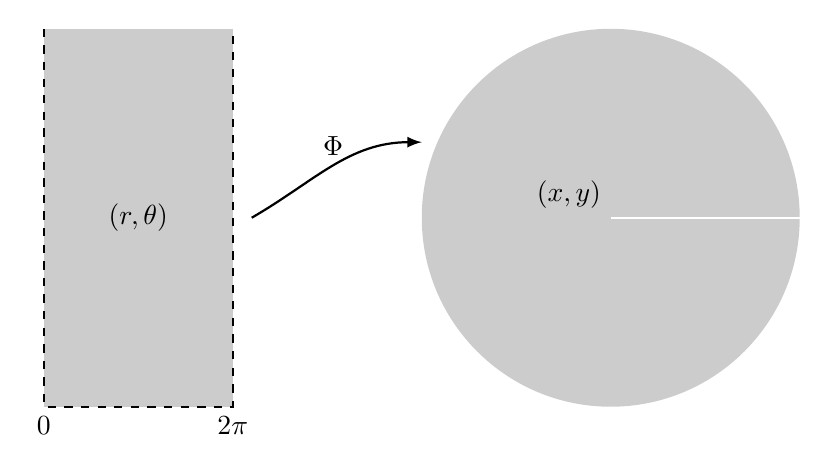
\begin{tikzpicture}[>=latex,scale=2.4]
        \fill[gray!40] (-0.5, -1) rectangle (0.5, 1);
        \draw[dashed, thick] (-0.5, 1) -- (-0.5, -1) node[below] {$0$} -- (0.5, -1) node[below] {$2\pi$} -- (0.5, 1);
        \fill[gray!40] (2.5, 0) circle (1);
        \draw[white, thick] (2.5, 0) -- (3.5, 0);
        \draw node at (0, 0) {$(r, \theta)$} node[above left] at (2.5, 0) {$(x, y)$};
        \draw[thick] (0.6, 0) edge[out=30, in=180, ->] node[above] {$\Phi$} (1.5, 0.4);
    \end{tikzpicture}
    \caption{坐标变换的几何直观}
    \label{fig:coordinate-transformation}
\end{figure}

\begin{example}{坐标变换}{}
    对于定义区域 $\Omega_1$ 和 $\Omega_2$ 如下:
    \[\Omega_1 = \mathbf{R}^2\setminus\{(x, y) \mid x\geqslant 0, y = 0\},\enspace \Omega_2 = \mathbf{R}_{>0}\times (0, 2\pi) = \{(r, \theta) \mid r>0, \theta\in(0, 2\pi)\}.\]
    我们熟悉的坐标变换 $x = r\cos\theta$,$y = r\sin\theta$ 就可以写成 \[\Phi\colon \Omega_2\to\Omega_1,\enspace \Phi(r, \theta) = (r\cos\theta, r\sin\theta).\]
    如\autoref{fig:coordinate-transformation} 所示. 由于在 $\Omega_1$ 上我们给定了 $(x, y)$ 作为坐标,在$\Omega_2$ 上我们给定了 $(r, \theta)$ 作为坐标,所以我们可以使用 Jacobi 矩阵表示上述映射的微分
    \[
        \mathrm{d}\Phi = J\Phi = \begin{pmatrix}
            \dfrac{\partial x}{\partial r} & \dfrac{\partial x}{\partial \theta} \\[2ex]
            \dfrac{\partial y}{\partial r} & \dfrac{\partial y}{\partial \theta}
        \end{pmatrix} = \begin{pmatrix}
            \cos\theta & -r\sin\theta \\
            \sin\theta & r\cos\theta
        \end{pmatrix}
    \]
    根据反函数定理,这个映射当然是可逆的.
\end{example}

这个例子告诉我们:坐标变换允许我们将被积区域进行变换,比如将圆或球转化成一个矩形,这样就可以极大简化运算. 更确切来说,对于原被积区域 $\Omega$ 上的函数 $f$,我们可以定义一个映射 $\varphi\colon \Sigma \to \Omega,\enspace \varphi(\Sigma) = \Omega$,使得我们只需要在现被积区域 $\Sigma$ 对复合函数 $f\circ\varphi$ 进行积分,函数的复合保证了积分区域转换的合法性,但是我们并不可以草率进行$\displaystyle\int\limits_{\Omega}f\,\mathrm{d}x = \int\limits_{\Sigma}f\circ \varphi\,\mathrm{d}x$ 的计算,因为对于 $\Omega$ 上的某一块体积元 $\sigma$,对与 $f$ 与坐标变换 $\varphi$ 下对应的 $\Sigma$ 上的体积元 $\sigma'$ 的体积并不一定相等,就好像对于上面例子中,将圆转化为矩形一样. 那么体积究竟变化了多少呢?这就是下面重积分换元法将要讨论的事情了.

下面,我们首先考虑坐标变换为线性映射的情况,再使用微分学的基本手法对一般的坐标变换做线性化并且估计误差.

\begin{enumerate}[label=(\arabic*)]
    \item 平移变换. 设 $v_0$ 为一个固定的向量,考虑仿射线性变换$\varphi\colon \mathbf{R}^n\to \mathbf{R}^n$,$\varphi(x) = x + v_0$. 而矩形的体积显然是满足平移不变性的,对于一个可求体积的矩形 $A\subset \mathbf{R}^n$,$\varphi(A)\subset \mathbf{R}^n$当然也是可求体积的,并且体积不变.

    \item 伸缩变换. 设 $\lambda_i\in\mathbf{R}\enspace(1\leqslant i\leqslant n)$,我们考虑线性映射 $\varphi\colon \mathbf{R}^n\to \mathbf{R}^n$ ,
          \[\varphi(x_1, x_2, \ldots, x_n) = (\lambda_1x_1, \lambda_2x_2, \ldots, \lambda_nx_n),\enspace (x_1, x_2, \ldots, x_n)\in \mathbf{R}^.\]
          矩形 $A = [a_1, b_1]\times [a_2, b_2]\times \cdots\times [a_n, b_n]$ 在 $\varphi$ 下的像仍为矩形,且体积为\[ \nu(\varphi(A)) = \vert\lambda_1\vert \vert\lambda_2\vert \cdots\vert\lambda_n\vert \nu(A) = \lvert \det\varphi\rvert \nu(A).\]

          将矩形 $A$ 换成一般的可求体积的图形,上述公式仍然成立,这可以根据下面的覆盖引理得出:

          \begin{lemma}{第一覆盖引理}{}
              设 $A$ 为 $\mathbf{R}^n$ 中的可求体积的有界集合,则任给 $\varepsilon > 0$,存在有限个矩形 $\{I_i\}$ 与 $\{J_j\}$ 使得
              \[\bigcup_i I_i\subset A\subset \bigcup_i J_j; \enspace \sum_i \nu(I_i) + \varepsilon > \nu(A) > \sum_j \nu(J_j) - \varepsilon.\]
              其中 $\{I_i\}$、$\{J_i\}$ 的内部分别互不相交.
          \end{lemma}

          \begin{figure}[h]
              \centering
              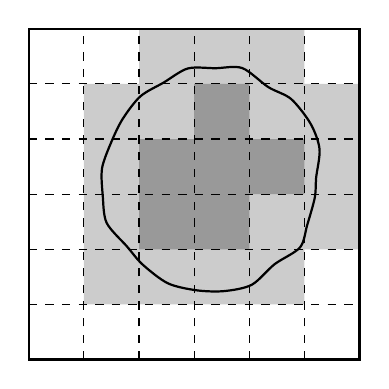
\begin{tikzpicture}[scale=0.7]
                  \pgfmathsetseed{42}

                  \fill[gray!40] (1, 1) -- (1, 5) -- (2, 5) -- (2, 6) -- (5, 6) -- (5, 5) -- (6, 5) -- (6, 2) -- (5, 2) -- (5, 1) -- cycle;
                  \fill[gray!80] (2, 2) -- (2, 4) -- (3, 4) -- (3, 5) -- (4, 5) -- (4, 4) -- (5, 4) -- (5, 3) -- (4, 3) -- (4, 2) -- cycle;

                  \draw[dashed] (0, 0) grid (6, 6);
                  \draw[thick] (0, 0) rectangle (6, 6);

                  \begin{scope}[shift={(3.3, 3.3)}]
                      \path[draw, thick] plot[domain=0:350, smooth cycle] (\x:1.9+0.2*rnd);
                  \end{scope}
              \end{tikzpicture}
              \caption{第一覆盖引理}
          \end{figure}

          \begin{proof}
              对于一个包含 $A$ 的一个矩形 $I$,首先可以定义一个示性函数 $\chi_A$,满足
              \[\chi(x) = \begin{cases}
                      1, & x\in A,    \\
                      0, & x\notin A.
                  \end{cases}\]
              这样 $A$ 的体积就可以表示为 $\nu(A) = \displaystyle\int_I\chi_A$. 因此对于任意的 $\varepsilon >0$,存在 $I$ 的分割 $\pi = \{I_{ij}\}$ 使得\[\left\lvert \sum_{ij}\chi_A(\xi_{ij})\nu(I_{ij}) - \nu(A)\right\rvert < \varepsilon,\enspace \forall \xi_{ij}\in I_{ij}.\]
              根据示性函数的定义,有 \[\sum_{ij}\inf_{\xi_{ij}\in I_{ij}}\chi_A(\xi_{ij})\nu(I_{ij}) = \sum_{I_{ij}\subset A}\nu(I_{ij}),\]
              所以,对于分割 $\pi$ 就有 \[\nu(A) - \varepsilon < \sum_{I_{ij}\subset A}\nu(I_{ij}) \leqslant \nu(A).\]
              同理可以有 \[\sum_{ij}\sup_{\xi_{ij}\in I_{ij}}\chi_A(\xi_{ij})\nu(I_{ij}) = \sum_{I_{ij}\cap A\neq \varnothing}\nu(I_{ij}),\]
              此时就有 \[\nu(A) < \sum_{I_{ij}\cap A\neq \varnothing}\nu(I_{ij}) < \nu(A) + \varepsilon.\]
              这就证明了第一覆盖引理,其中结论中的 $\{I_i\}$ 是 $I_{ij}\subset A$ 的那些 $I_{ij}$,$\{J_j\}$ 是 $I_{ij}\cap A\neq \varnothing$ 的那些 $I_{ij}$.
          \end{proof}

          这个证明的一个副产品就是:这些内部与 $\partial A$ 有非空交集的矩形的体积之和不会超过 $2\varepsilon$,这个结论也不失为一个良好的放缩.

    \item 正交变换. 正交变换就是我们所说的实数域上的等距同构. 对于正交变换 $O\in \mathcal{L}(\mathbf{R}^n)$ 其矩阵表示为 $O_M$,那么就有 $O_MO^\mathrm{T}_M = O_M^\mathrm{T}O_M = I_n$. 正交变换保持向量的模长不变,那么很自然的一点就是,我们可以大胆推断正交变换保持可求体积集合的体积不变,我们下面证明这一点. 首先需要第二覆盖引理.

          \begin{lemma}{第二覆盖引理}{}
              设 $A$ 是 $\mathbf{R}^n$ 中的可求体积的有界集合,则任给 $\varepsilon>0$,存在有限个 $n$ 维球体 $\{B_i\}$ 和 $\{B^j\}$,使得 \[\bigcap_iB_i\subset A \subset \bigcup_jB^j;\enspace \sum_j\nu(B^j) - \varepsilon < \nu(A) < \sum_j\nu(B_i) + \varepsilon,\]
              其中 $\{B_i\}$ 的内部互不相交.
          \end{lemma}

          \begin{figure}[h]
              \centering
              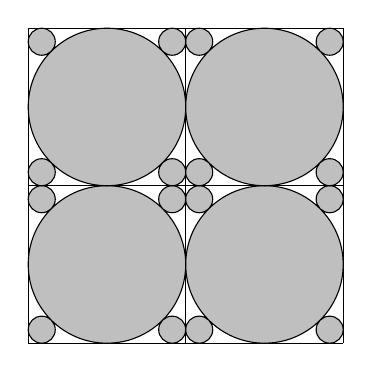
\begin{tikzpicture}[scale=2]
                  \draw (0, 0) grid (2, 2);
                  \foreach \i in {0.5, 1.5}
                  \foreach \j in {0.5, 1.5}
                  \draw[fill=gray!50] (\i, \j) circle (0.5)
                  \foreach \k in {45, 135, 225, 315} {($(\i, \j) + (\k:{sqrt(2)/(sqrt(2)+1)})$) circle ({(sqrt(2)-1)/(2+2*sqrt(2))})};
              \end{tikzpicture}
              \caption{第二覆盖引理}
          \end{figure}

          \begin{proof}
              首先设 $\nu(A)>0$. 我们先取一个矩形 $I = \left[a, b\right]^n$ 使得 $A\subset I$. 将 $I$ 作 $m^n$ 等分,当 $m$ 充分大的时候,完全包含于 $A$ 的小矩形 $\{I_i^1\}$ 的体积之和满足条件 \[\sum_i\nu(I_i^1) > \frac12\nu(A).\]
              矩形 $I_i^1$ 的内接球记为 $B_i^1$,记半径为 $1$ 的 $n$ 维球的体积为 $\omega_n$,根据球体的体积公式或者伸缩变换的结果,我们有 \[\sum_i\nu(B_i^1) = \frac{\omega_n}{2^n}\sum_i\nu(I_i^1) > \frac{\omega_n}{2^{n+1}}\nu(A).\]
              记 \[q = 1 - \frac{\omega_n}{2^{n+1}}\in(0, 1).\]
              由于 $A$ 与 $B_i$ 均可求体积,所以 $A \setminus \bigcup_iB_i^1$ 自然也可求体积(为什么?),因此 \[ 0 < \nu\left(A \setminus \bigcup_iB_i^1\right) < q\nu(A).\]
              我们对 $A\setminus \bigcup\limits_iB_i^1$ 重复上述过程,可以得到包含于 $A\setminus \bigcup\limits_iB_i^1$ 有限个小球体 $\{B_{i'}^2\}$ 使得 \[0 < \nu\left(A\setminus \bigcup_iB_i^1\setminus \bigcup_{i'}B_{i'}^2\right) < q\nu\left(A\setminus \bigcup_iB_i^1\right) < q^2\nu(A).\]
              将这一部分不断重复下去,对于任意的 $\varepsilon > 0$,由于 $q^k\to 0\enspace (k\to \infty)$,所以当 $k$ 充分大的时候,我们就得到内部互不相交的有限个 $n$ 维球体 $\{B_i\}$ 使得 \[0 < \nu\left(A\setminus \bigcup_iB_i\right) < q^k\nu(A) < n^{-n/2}\frac{\varepsilon}{2}.\]
              现在考虑对于 $\overline{A} = A\setminus \bigcup\limits_iB_i$,仍然考虑矩形 $I$ 的 $m^n$ 等分,当 $m$ 充分大的时候,存在着覆盖 $\overline{A}$ 的小矩形 $\{I^j\}$ 使得 \[\sum_j\nu(I^j) < \nu(\overline{A}) + n^{-n/2}\frac{\varepsilon}{2} < n^{-n/2}\varepsilon.\]
              矩形 $I^j$ 的外接球记为 $B_2^j$,那么就有 \[\sum_j\nu(B_2^j) = \frac{\omega_nn^{n/2}}{2^n}\sum_j\nu(I^j) < \frac{\omega_nn^{n/2}}{2^n}n^{-n/2}\varepsilon \leqslant \varepsilon.\]
              这就说明了 $\{B_i, B_2^j\}$ 就是覆盖 $A$ 的 $n$ 维球体,注意到最后一段的证明对于体积为零的情形同样适用,这就完成了第二覆盖引理的证明.
          \end{proof}

          注意,尽管我们通过两个覆盖引理刻画出了可求体积图形的性质,简单定义了一个粗糙的 Jordan ``测度'',但是我们仍然需要谨记:``有限个''这个性质在这里是至关重要的. 更加严格的测度论可以将其推广到 ``可数个'',可以在实分析等课程中学习.

          \begin{theorem}{}{}
              正交变换保持体积不变.
          \end{theorem}

          \begin{proof}
              注意到正交变换将 $n$ 维球映为 $n$ 维球,且球的半径不变,进而其体积不变. 根据第二覆盖引理,正交变换将零体积映为零体积集. 再注意到正交变换将集合的边界点映射为边界点,内点映射为内点,因此将可求体积的集合映为可求体积的集合. 再由覆盖引理及其正交变换保持球体体积变则可知正交变换保持可求体积的集合的体积不变.
          \end{proof}

    \item 一般的线性变换. 设 $\varphi\colon \mathbf{R}^n\to \mathbf{R}^n$ 为线性映射,在 $\mathbf{R}^n$ 的标准基下可以表示为 $n$ 阶方阵,这个方阵仍然记为 $\varphi$. 对于 $\mathbf{R}^n$ 中的可求体积的有界集合 $A$,我们考虑在 $\varphi$ 下的像 $\varphi(A)$. 首先,如果 $\det\varphi = 0$,那么 $\varphi$ 就将 $A$ 压缩成了被某一个超平面包含的集合,这样的集合体积为 $0$,所以我们只考虑 $\det\varphi\neq 0$ 的情况. 这时候 $\varphi\varphi^\mathrm{T}$ 就是正定对称矩阵,根据实谱定理,其可以对角化并且其特征值都大于零,所以其有一个正的平方根 $P$,这样 $\varphi\varphi^\mathrm{T}$ 就可以写为 \[\varphi\varphi^\mathrm{T} = P^2,\]
          其中 $P$ 当然也是正定对称的,且 $\det P = \lvert\det\varphi\rvert$. 这允许我们构造一个正交矩阵 $O = P^{-1}\varphi$,读者可以自行验证它是正交的.

          停下来看一下正定对称矩阵 $P$ 的性质:其对应的线性映射是一个正且自伴的线性映射,我们将其对角化为 $P = O\,\diag(\lambda_1, \lambda_2, \ldots, \lambda_n) O^\mathrm{T}$,其中 $\lambda_i > 0,\enspace 1\leqslant i\leqslant n$,且 $O$ 是一个正交变换. 根据正交变换与伸缩变换的结果,我们得到 \[\nu(P(A)) = (\det P)\nu(A).\]
          结合上面的分析,我们将一个非退化的线性映射 $\varphi$ 分解为一个正交变换与一个正定自伴映射,这就表明如果 $A$ 是可求体积的图形,那么 $\varphi(A) = P(O(A))$ 也是可求体积的,且有 \[\nu(\varphi(A)) = \nu(P(O(A))) = (\det P)\nu(O(A)) = (\det P)\nu(A) = \lvert\det\varphi\rvert \nu(A).\]
\end{enumerate}
简而言之,我们将上述分析总结为下面的定理:

\begin{theorem}{}{}
    对于一般的线性映射 $\varphi\colon \mathbf{R}^n\to \mathbf{R}^n$,与一个可求体积的图形 $A$,其像 $\varphi(A)$ 也是可求体积的,且有 \[\nu(\varphi(A)) = \lvert\det\varphi\rvert \nu(A).\]
\end{theorem}

现在我们要考虑比线性映射更一般的映射,根据``连续可微映射在某一点的局部性质与其在该点的微分的性质相同''这一核心原理,我们可以猜测对于某一点 $p$,如果 $\det J\varphi(p)\neq 0$,对于 $p$ 附近的一个非常小的可求体积的图形 $A$,有 $\nu(\varphi(A)) = \lvert\det J\varphi(p)\rvert \nu(A)$. 对这样的一个个小的面积元进行积分,就是重积分换元法的核心想法. 下面我们给出详细的证明.

设 $D\subset \mathbf{R}^n$ 为开集,$\varphi\colon D\to \mathbf{R}^n$ 为 $C^1$ 映射,根据拟微分中值定理,我们可以知道 $\varphi$ 是一个局部 Lipschitz 映射,也就是任取一个有界闭集 $P\subset D$ 与点 $x, y\in P$,存在 $\rho > 0$ 使得 \[\vert \varphi(x) - \varphi(y)\vert \leqslant \Vert J\varphi(\xi)\Vert \vert x - y\vert \leqslant \rho \vert x - y\vert.\]
所以下面讨论的主题就是如何对可求体积的集合 $A$ 在这样一个局部 Lipschitz 映射下的像 $\varphi(A)$ 的体积进行估计.

\begin{lemma}{}{}
    设 $\varphi\colon\mathbf{R}^n\to \mathbf{R}^n$ 为一个局部 Lipschitz 映射,亦即满足\[\Vert \varphi(x) - \varphi(y)\Vert \leqslant \rho \Vert x - y\Vert,\enspace \forall x, y\in\mathbf{R}^n.\]
    对于一个可求体积的集合 $A\subset \mathbf{R}^n$,如果 $A$ 为零测集,那么 $\varphi(A)$ 也是零测集;如果 $A$ 与 $\varphi(A)$ 都是可求体积的,就有 $\nu(\varphi(A)) \leqslant \rho^n\nu(A)$.
\end{lemma}

\begin{proof}
    设 $A$ 是零测集,则任给 $\varepsilon > 0$,存在至多可数个球体 $B_i = B_{r_i}(x^i)$ 使得 \[A\subset \displaystyle\bigcup_{i\geqslant 1}B_i,\enspace \sum_{i\geqslant 1}\nu(B_i) = \sum_{i\geqslant 1}\omega_n r_i^n < \varepsilon.\]
    由 $\varphi$ 是局部 Lipschitz 的可以得出 $\varphi(B_i) \subset B_{\rho r_i}(\varphi(x^i))$,所以 \[\sum_{i\geqslant 1}\nu(B_{\rho r_i}(\varphi(x^i))) = \sum_{i\geqslant 1}\omega_n (\rho r_i)^n = \rho^n\sum_{i\geqslant 1}\omega_n r_i^n < \rho^n\varepsilon.\]
    这就说明 $\varphi(A)$ 也是零测集.

    设 $A$ 和 $\varphi(A)$ 都是可求体积的,我们使用第二覆盖引理,对于任给的 $\varepsilon > 0$,存在有限个可以覆盖 $A$ 的 $n$ 维球体 $\{B_{r_j}^j\}$ 使得 \[\sum_j\omega_n r_j^n < \nu(A) + \varepsilon.\]
    所以此时 $\varphi(A)$ 被 $\{B_{\rho r_j}^j\}$ 覆盖,因此 \[\nu(\varphi(A))\leqslant \sum_{j}\omega_n (\rho r_j)^n = \rho^n\sum_j\omega_n r_j^n < \rho^n(\nu(A) + \varepsilon).\]
    通过 $\varepsilon$ 的任意性可以得出 $\nu(\varphi(A)) \leqslant \rho^n\nu(A)$.
\end{proof}

事实上,通过反函数定理,如果 $J\varphi$ 处处非退化,那么 $\varphi$ 将内点映射为内点,这就说明如果 $A$ 可求体积,并且 $\overline{A}\subset D$,那么我们对 $\partial \varphi(A)$ 进行放缩:\[\partial \varphi(A) = \overline{\varphi(A)}\setminus \varphi(A)^{\circ} \subset \varphi(\overline{A})\setminus \varphi(A^{\circ}) \subset \varphi(\partial A),\]
由 $A$ 可求体积可以得到 $\partial A$ 是零测集,所以 $\varphi(\partial A)$ 也是零测集,$\partial \varphi(A)$ 仍是零测集,所以 $\varphi(A)$ 就可求体积. 上面的定理只不过给出了 $\varphi(A)$ 体积的一个简单刻画,我们下面将 $\varphi$ 进行线性化并且进行误差估计. 取 $\delta > 0$ 使得 $K = \{x \mid d(x, A) \leqslant \delta\} \subset D$,并记 $C = \max\limits_{x\in K}\Vert J\varphi(x)\Vert$,回忆先前对线性映射与其线性化的映射之间的误差估计,我们可以直接得到下面引理:

\begin{lemma}{}{}
    沿用上面的记号,任给 $\varepsilon >0$,存在 $0<\eta <\delta$,使得当 $x\in A$,$d(x', x)\leqslant \eta$ 时,有 \[\Vert \varphi(x') - \varphi(x) - J\varphi(x)(x' - x)\Vert\leqslant \varepsilon\Vert x' - x\Vert.\]
\end{lemma}

\begin{lemma}{}{}
    沿用上面的记号,则当 $B\subset A$ 可求体积且 $d(B) < \eta$ 时,有 \[\nu(\varphi(B)) \leqslant \left(\lvert \det J\varphi(x)\rvert + O(\varepsilon)\right)\nu(B),\enspace x\in B.\]
\end{lemma}

\begin{proof}
    我们考虑线性变换 $L(y) = \left[J\varphi(x)\right]^{-1}(y - \varphi(x)) + x$ 并记 $F(y) = \varphi(y) - \varphi(x) - J\varphi(x)(x'-x)$,则 \[L\circ\varphi(x') = \left[J\varphi(x)\right]^{-1} F(x') + x'.\]
    于是当 $x', x''\in B_\eta(x)$ 的时候,\[L\circ\varphi(x') - L\circ\varphi(x'') = \left[J\varphi(x)\right]^{-1} (F(x') - F(x'')) + (x' - x'')\leqslant (1 + C\varepsilon)\Vert x' - x''\Vert.\]
    通过 $B\subset B_\eta(x)$ 可以得到 $\nu(L\circ\varphi(B)) \leqslant (1 + C\varepsilon)^n\nu(B)$,所以\[\nu(\varphi(B)) = \frac{\nu(L\circ\varphi(B))}{\lvert \det L\rvert}\leqslant \lvert \det J\varphi(x)\rvert \cdot (1 + C\varepsilon)^n\nu(B) = \left(\lvert \det J\varphi(x)\rvert + O(\varepsilon)\right)\nu(B).\]
    这样就得到了证明.
\end{proof}

\begin{theorem}{重积分换元法}{}
    设 $\varphi\colon D\to \mathbf{R}^n$ 为 $C^1$ 的一个单射,且 $J\varphi$ 处处非退化. 设 $A\subset D$ 为可求体积的集合,$\overline{A}\subset D$,$f$ 在 $\varphi(A)$ 上可积,那么\[\int_{\varphi(A)}f = \int_A f\circ \varphi\lvert \det J\varphi\rvert.\]
    特别地,\[\nu(\varphi(A)) = \int_A \lvert \det J\varphi\rvert.\]
\end{theorem}

\begin{proof}
    根据第一覆盖引理,不妨设 $A$ 为一个矩形,且 $f$ 非负,对于 $A$ 的任意一个分割 $\pi = \{A_{ij}\}$,我们有\[\int_{\varphi(A)}f = \sum_{i, j}\int_{\varphi(A_{ij})}f \leqslant \sum_{i, j}[\sup\limits_{\varphi(A_{ij})}f]\nu(\varphi(A_{ij})).\]
    对于任意的 $\varepsilon$ 当分割充分细,使得 $d(A_{ij})$ 小于某一个 $\eta$ 时,由上述的引理我们知道\[\int_{\varphi(A)}f \leqslant \sum_{i, j}\sup\limits_{A_{i, j}}(f\circ\varphi) \lvert\det J\varphi(\xi_{ij})\rvert \nu(A_{ij}) + O(\varepsilon) = \int_{A}f\circ\varphi\lvert\det J\varphi\rvert + O(\varepsilon).\]
    令 $\varepsilon\to0^+$ 可以得到\[\int_{\varphi(A)}f\leqslant \int_A f\circ\varphi\lvert\det J\varphi\rvert.\]
    根据反函数定理,$\varphi\colon D\to \varphi(D)$ 是可逆的,所以我们对于 $\varphi^{-1}$ 与 $\displaystyle\int_{A}f\circ\varphi\lvert\det J\varphi\rvert$ 进行类似的论证,可以得到 \[\int_{A}f \circ \varphi\lvert \det J\varphi\rvert \leqslant \int_{\varphi(A)}f\circ \varphi\circ\varphi^{-1}\lvert\det J\varphi\rvert \cdot\lvert \det J\varphi^{-1}\rvert  = \int_{\varphi(A)}f.\]
    综上所述,我们有\[\int_{\varphi(A)}f = \int_{A}f\circ\varphi\lvert\det J\varphi\rvert.\]这就完成了证明.
\end{proof}

这样,我们其实可以发现:重积分换元法的核心想法其实是研究\textbf{可求体积的图形在某一个映射下的体积是如何变化的}. 以这个想法为主线,配合\textbf{连续可微映射在某一点的局部性质与其在该点的微分的性质相同}这一核心原理,从线性映射到误差估计,我们就完成了重积分换元法的证明.

\begin{summary}

\end{summary}

\begin{exercise}
    \exquote[H. 格拉斯曼(Hermann Grassmann)]{但是,因为我将这些东西视作不仅是一个“量”,而且是一个“简单量”。也有其它的量是复合而成的,并且相对于其它的复合量相差一些简单量的加和。这些量通过更高级的形式的加和形成。}

    \begin{exgroup}
        \item % Schatten 范数 是 范数
        %   设 $A$ 为 $n$ 阶矩阵,定义 $A$ 的 Schatten 范数为 $\Vert A\Vert_s = \left(\sum_{i=1}^n\sigma_i^s\right)^{1/s}$,其中 $\sigma_i$ 为 $A$ 的奇异值. 证明 $\Vert A\Vert_s$ 是一个范数.
    \end{exgroup}

    \begin{exgroup}
        \item
    \end{exgroup}

    \begin{exgroup}
        \item
    \end{exgroup}
\end{exercise}

\chapter{线性代数与最优化问题}

\section{线性规划的几何}


\section{线性规划的对偶}


\section{下降方法}


\begin{summary}

\end{summary}

\begin{exercise}
    \exquote[艾伦·佩利(Alan J. Perlis)]{庸才无视复杂度,实用主义者忍耐它,有的人避免它,而天才消灭它.}

    \begin{exgroup}
        \item
    \end{exgroup}

    \begin{exgroup}
        \item
    \end{exgroup}

    \begin{exgroup}
        \item
    \end{exgroup}
\end{exercise}

\LUchapter{范畴论视角下的线性代数}

% 关于代数学的历史,最值得一读的文献大概是 J. Derbyshire 的 \emph{Unknown Quantity: A Real and Imaginary History of Algebra}. 这本书的写作风格轻松明快,不难卒读,其中历数的历史,笔者在此不再赘述. 而由于现代代数学卷帙浩繁,难以尽数,而且其中的大部分主题也远超笔者心力之所能及,在这里,仅仅就一些主要趋势泛泛而谈,有识见的读者可以自行翻阅文献,不必为笔者为方便理解所作的简化以及本身不完整的理解所累.

% 按照笔者的思路,我们将首先正式引入范畴论. 在范畴论的框架下,接下来我们要考虑的是代数与拓扑之间的联系,这会将我们引向两个截然不同的方向:同伦论(homotopy theory)和凝聚态数学(condensed mathematics). 前者相较后者历史较为悠久,正好够我们历数从 1950s 到现代的一些发展;后者则方兴未艾,可供读者一窥当代数学家的风貌. 至于一些未被纳入此框架的探讨和研究,代数数论将作为最后的讨论的切入口. 还有一些剩下的,例如群论、环论、表示论等主题的发展,则只能付之阙如了.

% 当然,还有一个被遗落的庞大的专题,就是在 Derbyshire 的书中开了个头的代数几何. 这一部分的探讨笔者无力完成,只能在此稍作提示——不过,在同伦论的部分中,我们也会见到其中的许多重要人物. 这个专题几乎是当代数学的前沿核心,但也正因为其核心地位,对它所作的任何不由杰出人物写下的讨论都显得有些不足,而且其研究所需的前置知识也远非本书所能及. 因此,在此我们只能无奈将其抛下,这并非轻视其重要性的表现.

这是本书的最后一章,也是最后一个未竟专题. 一切旅程都有终点,线性代数也不例外. 但是,终点同时也是一个起点,因此,在这里,我们将要引入现代数学中必不可少的一套语言——范畴论语言,并且使用这种方式来重述线性代数的一些概念,为本书画上一个句号. 可惜的是,因为篇幅有限,在这里不能重现利用范畴语言完成的全书所有内容的推导,但是我们会尽量走的远一些,同时也轻松一些. 在读者的代数基础尚且不算充足的时候,这一节的内容看起来可能有些抽象. 但如果在现代数学的路上走出更远,回头再来用这里的内容印证自己所学,相信读者依然会有所收获,这也就是未竟专题的未竟意义之所在.

在范畴语言引入之初,其提出者之一,Mac Lane 曾经下过一个断言. 他说,范畴论没有定理. 这是因为范畴论归根结底看起来只是一种“讲法”,正如我们在标题中所言,是一种“重述”,而非一套完全新颖的理论. 但是,这个断言很快就被打破了. 从本节会提及的 Yoneda 引理到本节不可能提及的 Freyd-Mitchell 嵌入定理,范畴论本身也逐渐发展成了一个生机勃勃的学科,并隐隐有成为数学基础的有力竞争者的趋势. 因此,最后,我们也希望读者思考,数学到底是什么?它是一种如范畴论所说,对对象和关系的研究,还是一种逻辑推导,抑或是一种直觉的形式化?如果读者在此方面有所意识,那么在未竟专题中走过的路也就都是有价值的.

\section{范畴、函子、自然变换}

范畴论的引入来自于 Samuel Eilenberg and Saunders Mac Lane \emph{General theory of natural transformations}, Trans. AMS, 58, p.p.: 231-294 (1945). 我们在此以现代的语言重述其概念,下面我们要呈现其中的三个核心定义:范畴、函子、自然变换.

\begin{definition}{}{}
    称以下资料为一个\term{范畴},记作 $\cC$:
    \begin{enumerate}
        \item 一族元素,每个元素称为其中的\term{对象},这一个族记作 $\Ob(\cC)$;我们将 $A \in \Ob(\cC)$ 简记作 $A \in \cC$;
        \item 一族 $A$ 到 $B$ 的箭头或者\term{态射} $\Hom_\cC (A, B)$,对于 $\Ob(\cC)$ 中的任意两个元素 $A, B \in \cC$,满足如下条件:
              \begin{enumerate}
                  \item 如果 $A, B, C \in \cC, \alpha \in \Hom_\cC (A, B), \beta \in \Hom_\cC (B, C)$,则存在复合 $\beta \circ \alpha \in \Hom_\cC(A, C)$;
                  \item 对于任意$D \in \cC, \gamma \in \Hom_\cC (C, D)$,都有\[
                            \gamma \circ (\beta \circ \alpha)= (\gamma \circ \beta) \circ \alpha;
                        \]
                  \item $\Hom_\cC (A, A)$ 中必有一个恒同元素,记作 $\id_A$,使得对于任意的$f \in \Hom_\cC (B, A)$,
                        \[\id_A \circ f = f \circ \id_B \]
              \end{enumerate}
    \end{enumerate}
\end{definition}

对这个定义,需要进行一些说明. 我们用“一族”的地方所指的未必是“一个集合”. 这是为了避免一些集合论上的麻烦,出现例如集合的集合之类的问题. 在范畴不会引起误会的情况下,我们将 $\Hom_\cC (A, B)$ 简记成 $\Hom (A, B)$,其中的元素 $f$ 也写成 $f\colon A \to B$ 或者 $A \stackrel{f}{\to} B$.

对于本书的读者而言,最熟悉的范畴无疑是线性空间的范畴. 准确地说,是域 $\F$ 上的有限维线性空间的范畴. 我们将其记作 $\FVect_\F$. 其中的对象就是所有的有限维线性空间,两个线性空间 $V, W$ 之间的态射 $\Hom (V, W) = \mathcal{L}(V, W)$. 另一个熟悉的范畴是 $\Set$,其中的对象就是所有集合,两个集合 $S, T$ 之间的态射就是从 $S$ 到 $T$ 的映射. 但是,出于习惯考量,当后面我们提及 $\Set$ 时,涉及的态射会变成从集合 $S$ 到 $T$ 的含入映射. 当然,范畴的对象并不总是这样“类似集合”的东西,虽然目前为止,这样理解已经足够了.

最后一个说明来自于结合律. 读者可能会认为,对于定义的第二条性质,最后的要求实属多余. 但实际上,如果我们只有抽象的点和箭头,很多性质也就无从谈起. 就像我们在学习线性空间的时候,它比起集合多了许多公理,因此也多了许多性质. 结合律实际上是范畴性质之根本,正如我们在下一个定义中会看到的一样.

\begin{definition}{}{}
    设 $\cC, \cD$ 为两个范畴. 称 $F$ 为 $\cC$ 到 $\cD$ 的一个\term{函子},如果:
    \begin{enumerate}
        \item 对 $\cC$ 中的每个对象 $A$ 它指派 $\cD$ 中的一个对象 $F(A)$;
        \item 对 $\Hom_\cC (A, B)$ 中的每个态射 $\alpha$ 它指派 $\Hom_\cD (F(A), F(B))$ 中的一个态射 $F(\alpha)$,满足
              \begin{enumerate}
                  \item 对于可复合的 $\alpha, \beta$ 都有 $F(\alpha \circ \beta) = F(\alpha) \circ F(\beta)$;
                  \item 对于任意 $A \in \cC$ 都有 $F(\id_A) = \id_{F(A)}$;
              \end{enumerate}
    \end{enumerate}
\end{definition}

最简单的函子的例子是一个范畴打到自身的恒同函子,它不会改变任何东西;以及 $\FVect_\F$ 到 $\Set$ 的忘却函子,它直接抛掉线性空间中的代数结构,只留下里面的元素. 现在我们考虑一个不那么平凡的例子:

\begin{example}{}{}
    考虑范畴 $\FSet$ 的对象是所有的有限集,其中的态射为含入映射. 则它到 $\FVect_\F$ 有一个显然的函子,是张成函子,我们将其记作 $\spa: \FSet \to \FVect_\F$. 它将一个有限集合映到由它张成的线性空间. 实际上,也就是将 $S = \{s_1, s_2,\ldots, s_n\}$ 映到一个形式和:

    \[
        \spa S = \left\{\sum_{i = 1}^n a_i s_i: a_i \in \F\right\}
    \]

    其上的线性空间运算都是显然的. 同样不难验证它将原来的含入映射映到一个线性映射,一个含入映射总是可以被对应到一个从子空间到原空间的嵌入.
\end{example}

另一个我们早就有所暗示的例子有点不同,它长得更加奇怪. 考虑一个范畴 $\cC$ 的对偶为将其中所有箭头反转的新范畴——不难验证它依然满足结合律,我们将其记作 $\cC^\mathrm{op}$,称为它的对偶范畴. 于是,我们发现,$\FVect_\F$ 到 $\FVect_\F^\mathrm{op}$ 有一个显然的函子,即对偶函子. 在对偶空间的部分中,我们已经验证了它满足函子的定义. 在较为古老的教科书中,这种打到对偶范畴的函子被称为反变函子,而上面定义的函子被称为共变函子,因为这类称呼已经淹没在历史的浪潮中了,所以我们也不会再使用了.

最后一个概念是最核心的,实际上也是范畴论被提出的初衷. 还记得上面提到的论文的标题吗?它叫做“自然变换的一般理论”,于是,下面我们就要说明,什么是自然变换. 这看起来可能会有点抽象:

\begin{definition}{}{}
    考虑两个函子 $F, G: \cC \to \cD$. 称这两个函子之间的\term{自然变换}是一族 $\cD$ 中的态射 $\theta = \{\theta_X\}$,其中 $X \in \cC, \theta_X: F(X) \to G(X)$,使得对于所有 $\cC$ 中的态射 $f$,下图交换:

    \begin{center}
        \begin{tikzcd}
            F(X) \rar["\theta_X"] \dar["F(f)", swap] & G(X) \dar["G(f)"] \\
            F(Y) \rar["\theta_Y", swap] & G(Y)
        \end{tikzcd}
    \end{center}

    通常,我们将其记成以下形式:

    \begin{center}
        \begin{tikzcd}
            \cC \rar[bend left=50, "F"{name=U}]
            \rar[bend right=50, "G"{name=D}, swap]
            & \cD
            \arrow[Rightarrow, from=U, to=D, shorten =2pt, pos=0.5, "\theta"]
        \end{tikzcd}
    \end{center}

    并将其称作\term{2-胞腔}. 在最后一节中,我们将重新讨论这个名词的含义.

\end{definition}

也许,我们应该采取一种更直观的看法来理解这一串概念,下面的一些概念来自于拓扑学,但并不严格,仅仅是提供一个比较方便的几何直观. 实际上,对拓扑和范畴论更加熟悉之后,读者会发现这个类比背后的深意.

\begin{figure}[htb]
    \centering
    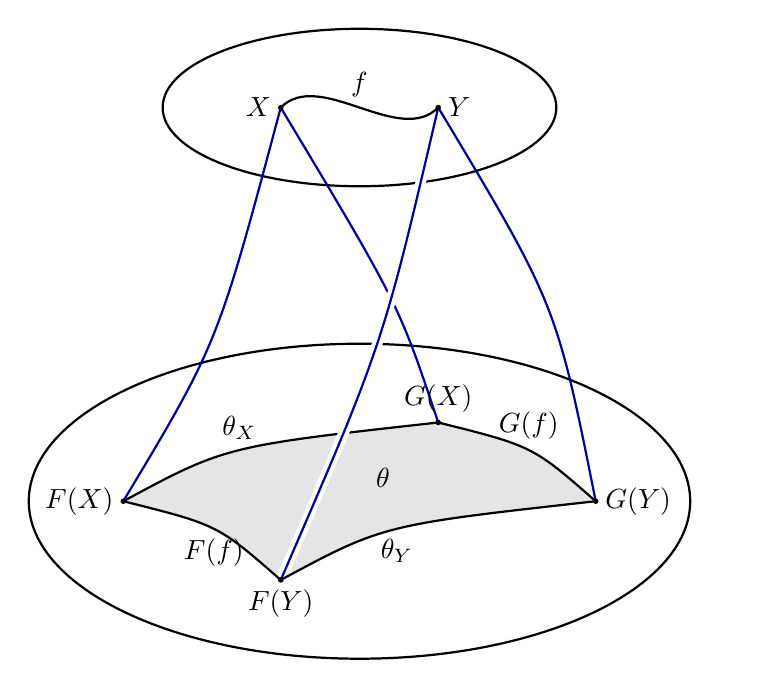
\begin{tikzpicture}
        \draw[thick] (0,3) ellipse (2.5 and 1)
        (0,-2) ellipse (4.2 and 2)
        node at (3, 3) {$\cC$}
        node at (4.7, -2) {$\cD$}
        coordinate (X) at (-1, 3)
        coordinate (Y) at (1, 3)
        coordinate (FX) at (-3, -2)
        coordinate (GY) at (3, -2)
        coordinate (GX) at (1, -1)
        coordinate (FY) at (-1, -3)
        coordinate (FX-GX-ct1) at (-1.7, -1.3)
        coordinate (FY-GY-ct1) at (0.3, -2.3)
        coordinate (FX-FY-ct1) at (-1.8, -2.3)
        coordinate (GX-GY-ct1) at (2.2, -1.3)
        coordinate (X-FX-ct1) at (-1.8, 0)
        coordinate (Y-FY-ct1) at (0.3, 0)
        coordinate (X-GX-ct1) at (0.5, 0.5)
        coordinate (Y-GY-ct1) at (2.5, 0.5);

        \fill[gray!20] (FX) .. controls (FX-GX-ct1) .. (GX) .. controls (GX-GY-ct1) .. (GY) .. controls (FY-GY-ct1) .. (FY) .. controls (FX-FY-ct1) .. (FX) -- cycle;

        \node at (0.3, -1.7) {$\theta$};

        \draw[thick] (FX) .. controls (FX-GX-ct1) .. node[above] {$\theta_X$} (GX) .. controls (GX-GY-ct1) .. node[above] {$G(f)$} (GY);
        \draw[thick,draw=blue!60!black] (X) .. controls (X-FX-ct1) .. (FX) (X) .. controls (X-GX-ct1) .. (GX);
        \draw[draw=white,double=blue!60!black,line width=1.5pt,double distance=0.8pt] (Y) .. controls (Y-FY-ct1) .. (FY);
        \draw[thick,draw=blue!60!black] (Y) .. controls (Y-GY-ct1) .. (GY);
        \draw[thick] (FX) .. controls (FX-FY-ct1) .. node[below] {$F(f)$} (FY) .. controls (FY-GY-ct1) .. node[below] {$\theta_Y$} (GY);
        \draw[thick] (X) .. controls (-.5, 3.5) and (.5, 2.5) .. node[above] {$f$} (Y);

        \node[left] at (X) {$X$};
        \node[right] at (Y) {$Y$};
        \node[left] at (FX) {$F(X)$};
        \node[right] at (GY) {$G(Y)$};
        \node[above] at (GX) {$G(X)$};
        \node[below] at (FY) {$F(Y)$};

        \foreach \point in {X, Y, FX, GX, GY, FY}
        \fill[black] (\point) circle (1pt);
    \end{tikzpicture}
    \caption{自然变换的几何直观}
    \label{fig:natural-transformation}
\end{figure}

首先,我们在一张纸上画两个面,表示两个范畴$\cC,\cD$. 在一个面上取两个点 $X, Y$,这是它上面的两个对象;然后,在另一个面上取四个点,分别表示 $F(X), F(Y), G(X), G(Y)$,即两个函子$F,G$在这两个点$X,Y$的取值. 注意,实际上两个函子分别是两个面之间的映射,如果把原像和像用线连接,展开来看的话,大概能看成是纸面上和纸面下的两张带有纹路的曲面. 然后,自然变换就是这两个曲面之间的连线$\theta$,对应到交换图上来,就是图中阴影区域的四条边. 实际上,我们的条件就是要求,这两族曲面$F, G$的结构和曲面之间的结构$\theta$都具备合适的连续性,如\autoref{fig:natural-transformation},这个东西在拓扑学中一般称为\term{同伦}.

在实践中,我们一般会称态射 $\theta_X$ 对于 $X$ 来说是自然的、典范的,或者说它满足函子性. 我们来看两个例子:

\begin{example}{}{}
    一个线性空间到某个商空间的投影映射. 考虑所有包含子空间 $U$ 的有限维线性空间. 显然,它们构成一个范畴,其间的态射定义为限制在 $U$ 上为恒同映射的线性映射,我们将这个东西记作 $\FVect_\F^U$.

    实际上,我们在说的是,考虑一个函子 $p\colon \FVect_\F^U \to \FVect_\F$ 将线性空间 $X$ 映到线性空间 $X/U$,另一个函子 $i\colon \FVect_\F^U \to \FVect_\F$ 将线性空间 $X$ 映到线性空间 $X$ 自身. 态射的映射都是显然的. 接下来,我们要表明存在一个自然变换 $\theta: i \to p$.

    现在,取任意的 $f\colon X \to Y$ 为 $\FVect_\F^U$ 中的态射,则我们需要使其交换的图表如下:

    \begin{center}
        \begin{tikzcd}
            X \rar["\theta_X"] \dar["f", swap] & X/U \dar["f/U"] \\
            Y \rar["\theta_Y", swap] & Y/U
        \end{tikzcd}
    \end{center}

    其中 $f/U$ 表示诱导的商映射,我们在不变子空间那一节中有所提及. 其中的 $\theta_X$ 和 $\theta_Y$ 就是我们通常称的典范投影,这也就是为什么这个投影被称为典范的.
\end{example}

下一个典范的结构我们也已经有所提及,它事关双对偶空间. 为了方便起见,对于函子 $F: \cC \to \cD$,我们记 $F^\mathrm{op}: \cC^\mathrm{op} \to \cD^\mathrm{op}$,它和原来的函子其实毫无差别,只有一点形式上的不同. 记对偶函子为 $-^*$,这是因为我们通常用 $V^*$ 表示对偶的空间,$f^*$ 表示对偶映射. 那么,我们就有 $(-^*)^\mathrm{op} \circ -^*$ 是典范同构. 这个事情的证明也是检查交换图,我们早已构造了这样的映射,也就是所谓的到双对偶空间的典范同构.

最后一个例子稍微有点特别,为了给出这个例子,我们需要定义一个与自然变换稍微有点不同的东西,强名之曰自然反变换\footnote{英文为 dinatural transformation,这个翻译稍微有点奇怪,但凑合用. }. 它的目标实际上是处理一些反变函子的情形,其它定义完全一致,不过它要求:$F: \cC \to \cD, G: \cC \to \cD^\mathrm{op}$,而它对应的交换图是:

\begin{center}
    \begin{tikzcd}
        F(X) \rar["\theta_X"] \dar["F(f)", swap] & G(X)\\
        F(Y) \rar["\theta_Y", swap] & G(Y) \uar["G(f)", swap]
    \end{tikzcd}
\end{center}

那么正如读者所料,我们要给出的结果就是:

\begin{example}{}{}
    不存在从一个线性空间到其对偶空间的非零自然反变换.

    现在,我们需要考虑下面的交换图:

    \begin{center}
        \begin{tikzcd}
            X \rar["\theta_X"] \dar["f", swap] & X^*\\
            Y \rar["\theta_Y", swap] & Y^* \uar["f^*", swap]
        \end{tikzcd}
    \end{center}

    我们知道,不管 $X$ 怎么取,总能取到一个 $f$ 使得 $f$ 将 $X$ 中的所有元素映到 $Y$ 中的零元,而参照我们的定义,这时的 $f^*$ 取值只有 $X^*$ 中的零元,因此,$\theta_X$ 为了让这个图交换,只能让所有元素映到零元.
\end{example}

可见在选取了合适的形式化方法之后,这些看上去无从下手的概念的证明变得无比单纯. 这实际上在表明,从一个空间到它的对偶空间不存在典范的同构.

\section{范畴论的构造}

单单是范畴、函子和自然变换显然什么都不能给出. 现在,我们无非是形式化了一些原来就已经说出的东西,顶多是最后对自然性的表述稍稍有些新意. 范畴论最核心的点实际上在于,它告诉了你很多被定义的东西实际上有其他的定义方式,这就是我们在这一节会讨论的内容.

\subsection{单态射、满态射和同构}

当我们在描述映射的时候,我们通常会讨论它是单的,满的,还是同构. 正如前面矩阵空间中关于指数映射的讨论中所表明的那样,这个性质实际上是非常不平凡的. 因此,这些性质应当在范畴论中得到恰当的推广——但是,时刻记住,现在我们的对象不同于以往我们做操作的集合,虽然我们还是能够从中汲取灵感.

先考虑集合的情况. 单射在我们看来,是如果像相同则原像相同,也就是说,每个原像集中的元素都有不同的像. 那么,就应当存在一个函数把它翻译回去,使得它在原像集上是恒同映射,也就是说:

\begin{lemma}{}{}
    考虑集合 $S, T$,一个函数 $f\colon T \to S$ 是单射当且仅当存在映射 $g\colon S \to T$ 使得 $g \circ f = \id_T$.
\end{lemma}

证明如上所述,形式化的写法留给读者,对偶地,我们就有:

\begin{lemma}{}{}
    $f\colon T \to S$ 是满射当且仅当存在映射 $g\colon S \to T$ 使得 $f \circ g = \id_S$.
\end{lemma}

而后面的这个定义是纯粹用箭头完成的,因此,它就能被推广到态射的情形:

\begin{definition}{}{}
    考虑范畴 $\cC$ 和其中的态射 $f\colon A \to B$.
    \begin{itemize}
        \item 称 $f$ 是\term{单态射},如果存在 $g\colon B \to A$ 使得 $g \circ f = \id_B$;
        \item 称 $f$ 是\term{满态射},如果存在 $g\colon B \to A$ 使得 $f \circ g = \id_A$;
        \item 称 $f$ 为\term{同构},如果存在 $g\colon B \to A$ 使得 $f \circ g = \id_A$ 且 $g \circ f = \id_B$;
        \item 如果 $A$ 和 $B$ 之间存在一个同构,则称 $A$ 和 $B$ 同构.
    \end{itemize}
\end{definition}

读者不难发现,恒同映射是一个同构. 这样的结构看上去就像一个逆元. 如果所有的态射都是同构,那么如果所有对象构成集合,态射也构成集合(这是为了避免一些集合论纷争),则我们将这个范畴构成一个\term{群胚}或者\term{广群}. 其态射集满足某种意义上的群结构. 实际上,在习题中我们会更进一步地发现相关的性质.

这里有一个麻烦的事情:同构一定既是单态射又是满态射,但既是单态射又是满态射的态射不一定是同构. 如果后者成立,则我们将这个范畴称为平衡范畴. 实际上,在通常的情形下,这个性质都是成立的.

\subsection{泛性质:始对象和终对象}

我们知道,一个范畴就是对象和箭头,那么,下面的定义看起来就很合乎情理:我们要选出箭头比较特殊的那些对象.

\begin{definition}{}{}
    称一个对象 $A \in \cC$ 为始对象,如果对于任意 $B \in \cC$ 都有 $|\Hom_\cC (A, B)| = 1$. 终对象是对偶范畴中的始对象. 如果一个对象既是始对象又是终对象,我们称其为零对象.
\end{definition}

注意,终对象的定义和始对象是完全对偶的,所以,很多时候我们其实不太区分这两种对象,它们具备的 $|\Hom_\cC (A, B)| = 1$ 的性质我们往往称为泛性质. 一般的,泛性质成立表明它实际上是一个定义性的东西:

\begin{theorem}{}{}
    所有始对象都是同构的、所有终对象都是同构的.
\end{theorem}

证明过于显然,留作读者练习. 重要的是例子:$\FVect$ 中,$\{1\}$ 是零对象. 这实际上说明了这个玩意的特殊性,但我们对它的特殊性早已习以为常. 剩下的一些例子我们会在后面的构造中一一给出——实际上,所有不太平凡的例子都要求我们构造一些更为奇特的范畴.

\subsection{Hom 函子和 Yoneda 引理}

注意到,如果 $\cC$ 和 $\cD$ 都是范畴,则 $\cC \times \cD$ 也是一个范畴,其上的对象和态射都是显然的. 我们首先考虑这样一个函子:
\[
    \Hom: \cC^\mathrm{op} \times \cC \to \Set
\]

它将对象 $(c, c')$ 映到它们之间的态射集 $\Hom_\cC(c, c')$,而将态射 $(f: c \leftarrow d, f': c' \to d')$ 映到一个 $\Hom_\cC(c, c') \to \Hom_\cC(d, d')$ 的映射,以复合的形式:
\[
    \Hom(f, f')(q: c \to c') = f' \circ q \circ f
\]

这个东西看起来乌七八糟的,但是在后面谈到张量积的时候,这个定义会体现出一个非常明显的性质. 在此,我们考虑另一种

\subsection{伴随函子}

\subsection{逗号范畴}

\subsection{和与积、极限和余极限}

\subsection{纤维化和余纤维化}

\section{幺半范畴及其性质}

\subsection{函子范畴和单子}

\subsection{Beck 单子化定理*}

\subsection{张量积}

\section{2-范畴一瞥}

\subsection{伴随和伴随}

\subsection{作为 2-极限的逗号范畴}

\subsection{走向无穷范畴:为什么我们需要套娃?}

\begin{exercise}
    \exquote[——《收获与播种》,格罗滕迪克]{每一门科学,当我们不是将它作为能力和统治力的工具,而是作为我们人类世代以来努力追求的对知识的冒险历程,不是别的,就是这样一种和谐,从一个时期到另一个时期,或多或少,巨大而又丰富:在不同的时代和世纪中,对于依次出现的不同的主题,它展现给我们微妙而精细的对应,仿佛来自虚空。}

    \begin{enumerate}  % 若不需要编号,则直接使用 enumerate 环境
        \item 证明以下两个态射的性质:
        \begin{enumerate}
            \item 如果 $A$ 与 $B$ 同构,那么 $A$ 与 $B$ 之间的同构映射是唯一的;
            \item 函子保持态射的单、满性质.
        \end{enumerate}
    \end{enumerate}
\end{exercise}


\LUgroupsancheck

\makeatletter
\let\chapter\@std@chapter
\let\@std@chapter\relax
\makeatother

\backmatter
{\small
\printindex
\printindex[sym]
}

\end{document}
